\documentclass{mprop}
\usepackage{graphicx}
\usepackage{hyperref}
\usepackage{url}
\usepackage{amsmath}
\usepackage{caption}
\usepackage{epigraph}
\usepackage{tikz}
\usepackage{gantt}
%\uspackage{amssymb,amsmath}
%\usepackage{fancyvrb}
%\usepackage[final]{pdfpages}

% alternative font if you prefer
%\usepackage{times}

% for alternative page numbering use the following package
% and see documentation for commands
%\usepackage{fancyheadings}

% For MetaPost diagrams from Dia
\DeclareGraphicsRule{.1}{mps}{*}{}

% Inspirational Quote type setting
\makeatletter
\newenvironment{chapquote}[2][2em]
  {\setlength{\@tempdima}{#1}%
   \def\chapquote@author{#2}%
   \parshape 1 \@tempdima \dimexpr\textwidth-2\@tempdima\relax%
   \itshape}
  {\par\normalfont\hfill--\ \chapquote@author\hspace*{\@tempdima}\par\bigskip}
\makeatother

\begin{document}

%%%%%%%%%%%%%%%%%%%%%%%%%%%%%%%%%%%%%%%%%%%%%%%%%%%%%%%%%%%%%%%%%%%
\title{Securing and Integrating the IoT with a Smart Home Router}
\author{Fergus W. Leahy}
\date{16/12/2013}
\maketitle
%%%%%%%%%%%%%%%%%%%%%%%%%%%%%%%%%%%%%%%%%%%%%%%%%%%%%%%%%%%%%%%%%%%

%%%%%%%%%%%%%%%%%%%%%%%%%%%%%%%%%%%%%%%%%%%%%%%%%%%%%%%%%%%%%%%%%%%
\tableofcontents
\newpage
%%%%%%%%%%%%%%%%%%%%%%%%%%%%%%%%%%%%%%%%%%%%%%%%%%%%%%%%%%%%%%%%%%%

%%%%%%%%%%%%%%%%%%%%%%%%%%%%%%%%%%%%%%%%%%%%%%%%%%%%%%%%%%%%%%%%%%%
\section{Introduction}
\label{sec:introduction}

\begin{chapquote}{Mark Weiser, \textit{The Computer for the Twenty-First Century, 1991}}
    ``The most profound technologies are those that disappear. They weave themselves into the fabric of everyday life until they are indistinguishable from it.''
\end{chapquote}

The modern home is becoming increasingly filled with a variety of \textit{connected} devices (laptops, tablets, phones, set-top boxes etc.), providing a myriad of different services to users within the home. On top of this, with the introduction of smart phones and wearable devices, we too are starting to carry around our own personal network of devices everywhere we go, brushing past many others in our daily lives at home, work and on the street. Although all connected to the Internet, these devices are often encapsulated within their own environment and ecosystem, unable to interconnect, creating a fractured and often complex user experience. 

Making matters more interesting, the Internet of Things paradigm is once again becoming a field of great interest due to the advent of cheap, low-power wireless embedded devices \cite{2013IoT}. However, not much consideration has been made for how these Things should be integrated into the existing home network, with many approaches opting to simply bridge the device to the cloud (\cite{SmartThings}, \cite{Twine}, \cite{IETF_CORE}), with obvious concerns for security, privacy and up-time.

As these devices enter our homes and pockets, bringing with them their own ecosystems, the user is faced with the increasingly difficult burden of managing them and their ecosystems \cite{brundell2011w}, \cite{brown2013multinet}. Due to the sheer number and diversity of these devices, many of which will provide overlapping services and functionality, problems arise with respect to how these devices cooperate, as well as how to ensure that the user's network and information stays secure against new and unanticipated threats.

In order for these multiple layered networks of devices to truly fade away into the fabric of our everyday lives, a platform and relevant protocols need to be engineered to not only support this heterogeneous network securely, but also aid the user in managing both the network and the privacy of their information.

The Homework home router platform\cite{HomeworkControl} was created to address these issues. Rather than assume every user is a network administrator, the project investigated the needs and abilities of the average user in order to propose the future of home networking, re-inventing the protocols, models and architectures to truly suit the home environment. This re-invention of the home router allows a user to easily install, manage and use their home network, without the need of a Cisco qualification.

In regards to the Internet of Things development, previous work demonstrated that it was in need of a suitable protocol in order to meet the specific needs of a network of Things \cite{KNoT}. Thus, a new protocol was designed and implemented, which could not only run on the most constrained battery-powered devices (8MHz), but it could also efficiently scale to support hundreds of Things within the same network.

%TODO: WRITE MORE LINKY LINKY

%briefly explain the context of the project problem

%%%%%%%%%%%%%%%%%%%%%%%%%%%%%%%%%%%%%%%%%%%%%%%%%%%%%%%%%%%%%%%%%%%

\section{Statement of Problem}
\label{sec:statement_of_problem}
Whilst there have been many attempts, both past and recent, to create the perfect Internet of Things network for the home, all still exhibit several issues. This section will first present a typical user scenario to provide a context for this problem, then discuss several of the issues found in existing work, both our previous work and others', which provide the motivation for this project.

\subsection{A Scenario} % (fold)
\label{sub:scenario}
In order to establish the context of the problem, a typical user scenario has been created to demonstrate a typical novice user purchasing a new Thing and attempting to integrate it into their network securely with minimal knowledge and effort.

\textit{Bob buys a new Thing, a motion sensor, from a shop and brings it home. He wants to connect it to his currently existing home network. To do so, Bob turns on the Thing and presses the connect button on both the Thing and his home router. Using his tablet/PC Bob is able to view the newly available Things in the network that he can connect to, in which he can see his new Thing. Bob is able to view various information about the Thing, including it's type, manufacturer, functions etc. Bob selects the Thing he wants to connect to the network and within a minute the new thing is now part of the network and he can then customise how he wants to use it in the network.}

\subsection{The Problem} % (fold)
\label{sub:the_problem}
The Internet of Things protocol created in \cite{KNoT} proved to be a successful proof-of-concept; however, in order for it to be considered for deployment and integration into existing homes, two main issues need to first be addressed.

\subsubsection{Security} % (fold)
\label{ssub:security}

The initial design of the IoT protocol didn't consider security due to time constraints; however, because not only can such rich and sensitive data can be gathered about the user and their home from Things(devices), but the closed loop of control can be affected by illegal packet injection, to negatively alter its behaviour; therefore it becomes extremely important to not only protect the data from unauthorised access, but also protect the network itself. As demonstrated in the scenario, a user may want to purchase any kind of compatible Thing from a shop and then want bring it into their home network with minimal effort. The Thing itself would have no prior knowledge of the network and needs a secure mechanism to enter the network without compromising the rest of the network or exposing its own data to unauthorised users. 

Presented below is a summary of the typical attacks targeted towards WSNs, and in this case an IoT.
\begin{enumerate}
  \item \textbf{Eavesdropping} - An attacker observes the unencrypted traffic between the various devices in the network, and uses this information for illegitimate purposes. This needs to be prevented due to the richness, coverage and sensitivity of the data captured within an IoT, which could be used to perform serious physical attacks, spying, as well as have other serious consequences. Therefore, it's necessary to encrypt all traffic where possible, so that only legitimate participants may observe the information traversing the network.
  \item \textbf{Unsanctioned participants} - An attacker infiltrates the network masquerading as a legitimate participant, enabling it to spoof traffic, such as events and commands, as well as observe other traffic. Such an attack would enable an attacker to spy on and manipulate the network of Things, which could lead to various damaging consequences, ranging from energy waste, to more serious home security issues such security locks being disabled enabling other possible crimes.
  \item \textbf{Node capture} - Due to the placement of Things, sometimes outwith the protective confines of a home or building, they can become vulnerable to an attacker capturing them. Once captured, it may be possible to extract encryption keys, illegally modify the functionality and also replace nodes with maliciously modified ones.
  \item \textbf{Denial of service} - An attacker attempts to block or overwhelm the target, so that legitimate requests to contact the target will be unsuccessful. In the case of WSN this can occur from RF jamming, or by a packet based overload where the target is forced to continuously process computationally expensive packets for an extended period of time, such as with asymmetric cryptographic operations. 
\end{enumerate}

The attack vectors to be tackled by this project will be discussed in section \ref{ssub:attack_vectors}.

% subsubsection security (end)

\subsubsection{Integration} % (fold)
\label{ssub:integration}

The current implementation exists as a standalone library with several demo applications. Integration of the IoT protocol into a more powerful and user-friendly platform is necessary to harness the full power of a network of Things. The integrated platform would then be able to discover and connect to hundreds of available Things, subscribe and log events from the sensors, and using user customised rules, run automata to detect if these rules are met and then publish commands to actuators in the network to perform actions within the home.
% subsubsection integration (end)

\subsection{Intranet of Things vs Internet of Things} % (fold)
\label{sub:intranet_of_things}

As described earlier in section \ref{sec:introduction}, many previous deployments of Internet of Things networks have taken a cloud first approach \cite{SmartThings, Twine}. Whilst this yields certain benefits, such as easy external access and integration with other services \cite{IFTTT, Xively}, it also poses several questions regards data security, privacy and up-time. For this project, the focus will be on developing a home first platform, in which all Things communication will be kept local, with no cloud processing involved; thus a more suitable name, the Intranet of Things, will be used for the duration of this project. 
% subsection intranet_of_things (end)

% subsection the_problem (end)
\subsection{Project Outcomes} % (fold)
\label{sub:project_outcomes}

Outcomes of the project:
\begin{itemize}
  \item[-] An extended IoT protocol with sufficient security to prevent eavesdropping and unsanctioned devices.
  \item[-] An extended home information platform (Homework), with the IoT controller role implemented, enabling capturing of IoT events from sensors and creation of commands for actuators.
  \item[-] Use of Homework's automata to implement closed loop control of Things in the home, subscribing to sensor events, processing rules and publishing to actuators to perform actions within the IoT.
\end{itemize}
% subsection subsection_name (end)

% clearly state the problem to be addressed in your forthcoming project. Explain why it would be worthwhile to solve this problem.

\subsection{Structure} % (fold)
\label{sub:structure}
The rest of this proposal is structured in the following way. Section 3 surveys previous work on the field of wireless sensor networks security, home networks and Internet of Things systems and protocols. Section 4 takes what has been learnt from the literature survey and proposes a solution to solve the problem described above. Lastly, section 5 discusses the work plan outlined for the implementation and evaluation part of the project, for the second half of the year.
% subsection structure (end)

%%%%%%%%%%%%%%%%%%%%%%%%%%%%%%%%%%%%%%%%%%%%%%%%%%%%%%%%%%%%%%%%%%%

\section{Literature Review}
This section discusses previous work on Internet of Things protocols, WSN security and home networking which provides the motivation and possibly aids in solving the previously mentioned issues.

\subsection{State-of-the-art IoT Protocols} % (fold)
\label{sub:state_of_the_art_iot_protocols}
Over the last 20 years, the Internet of Things has developed and evolved continuously, from 20 years ago where it was the concept of using barcodes, and later RFID\cite{K.Ashton}, to track items in a warehouse, to today where our home appliances are filled with ``smart'' electronics, able to sense, react and notify the user of events, such as the washing machine finishing a load. Whilst the Internet of Things has been around for quite some time, under various guises, it's yet to become commercially successful and see wide-spread deployment; Many believe that 2013 is the year that the Internet of Things will truly take off and become ubiquitous in our daily lives\cite{2013IoT}.

The rest of this section will discuss the various different attempts made to create Internet of Things networks in the home.

\subsubsection{Smart Things} % (fold)
\label{ssub:smart_things}
Launched in 2012, the SmartThings platform aims to allow the user to turn any ordinary object in the home into a ``Smart'' object by giving it the ability to connect to the Internet. The platform consists of a central hub connected to the Internet, containing a low-power Zigbee radio, from which it connects to an array of SmartThings accessories as well as many pre-existing third party Zigbee devices. Some of these accessories include motion detectors, moisture sensors, vibration detectors, power-plug switches as well as many others. The user can then view and interact with their Smart Things through the cloud service via an Internet-connected PC or a smartphone, allowing them to either control the devices directly or set-up rules/schedules for devices.

\begin{figure}[h!]
\centering
    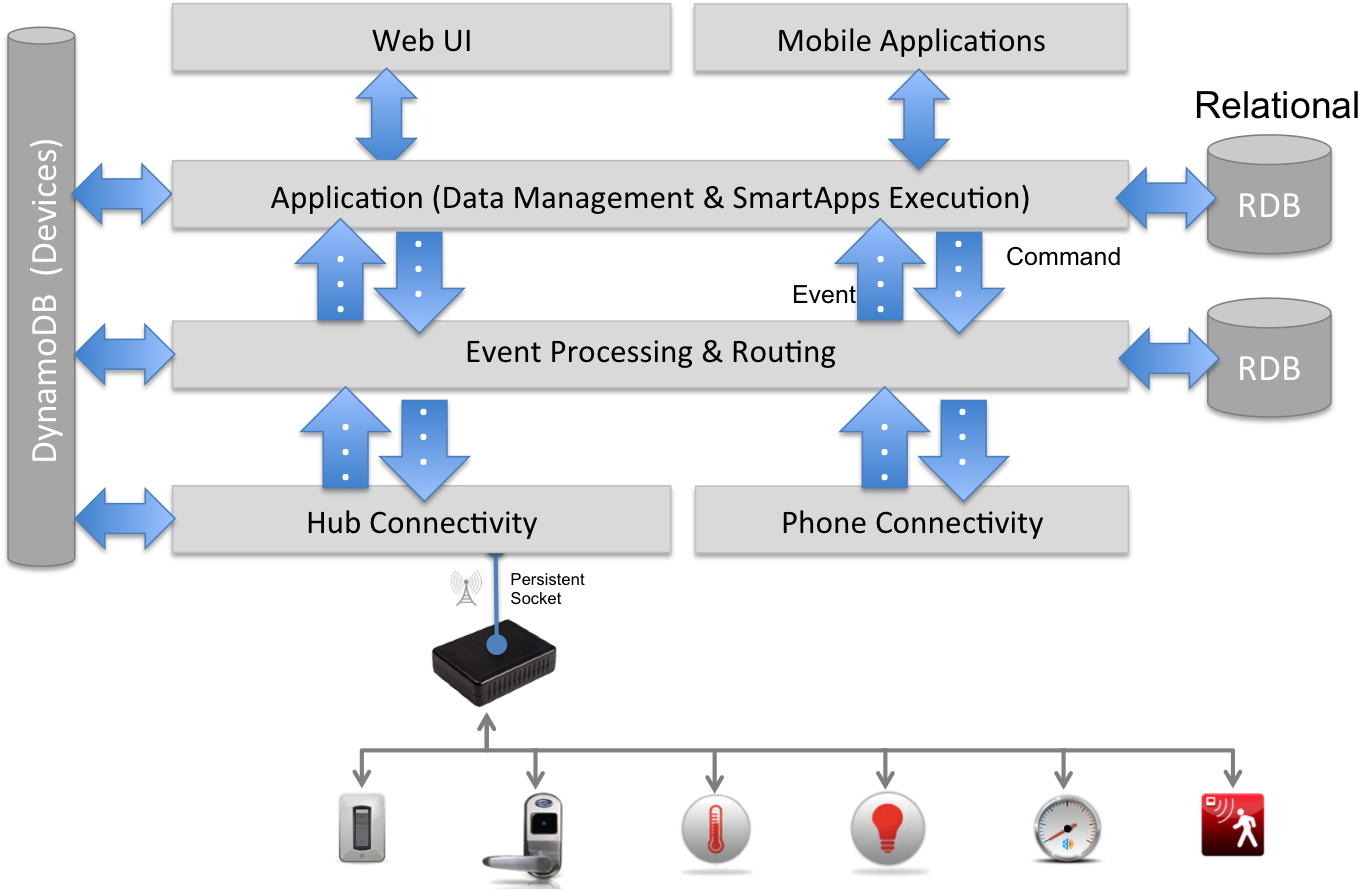
\includegraphics[scale=0.4]{images/smartThingsCloudFirstDiagram.png}
    \caption[]{Smart Things - Cloud approach\footnotemark}
    \label{fig:cloud}
\end{figure}
\footnotetext{Image from Smart Things developer support: \url{https://support.smartthings.com/entries/21603009-Device-Types-Capabilities-Attributes}}

As shown in figure \ref{fig:cloud}, Smart Things takes a cloud approach, offloading all processing to the cloud, leaving the hub to just act as a gateway and translator between the Things and the cloud. By utilising the cloud in this way, it enables the hub to be a very simple and low-power device, reducing both the purchasing and running costs for the user. It also allows the user to access their network of Things from anywhere, at any time, which would otherwise be difficult to do in a local approach. 

However, the cloud approach also has several drawbacks. By offloading the entire processing needs of the network, as show above, the network of Things becomes vulnerable to failure if either the network fails or is unresponsive, or if the cloud service fails or goes down for maintenance. Another issue is the privacy of the user's data; How safe is the data in the cloud and how secure are the services they make available for users to interact with their devices with. There have been many examples of online services that have been attacked, leaking user data and/or shutting down for extended periods of time \cite{Playstation, Amazon, Google}.

Talk about integration of two home networks.


% Currently, there is no information on how the underlying protocol for connecting the SmartThings to the hub works, but at the time of writing, the current implementation uses a ``cloud first'' approach. This means that rather than the hub wiring all devices together based on the rules and schedules set up by the user, all the intelligence of the network is being handled in the cloud. This brings about the problem of Internet connectivity, with two points of failure, either the user or the cloud. From the user's standpoint, an Internet connection might not be available where the hub is located, or the user could have a faulty, slow or non-permanent connection, which renders all the SmartThings devices into dumb devices. In contrast to this, because of the reliance on the cloud, if the cloud service provider experiences downtime then all SmartThings users devices become dumb devices. In cases where these devices are used for security and safety, dire consequences could result.
% subsubsection smart_things (end)

\subsubsection{CoRE CoAP HIP-DEX} % (fold)
\label{ssub:core_coap}

% subsubsection core_coap (end)
\subsubsection{KNoT} % (fold)
\label{ssub:knot}

% subsubsection knot (end)
% subsection state_of_the_art_iot_protocols (end)

\subsection{Home networking} % (fold)
\label{sub:homework_smart_home_router}
\textbf{Discuss Homework router and cache db}
% subsection homework_smart_home_router (end)

%%%%%%%%%
\subsection{WSN Security - Symmetric Cryptography} % (fold)
\label{sub:tinysec_minisec_contikisec}
Substantial research has been carried out to secure WSNs, to ensure data within the network can't be compromised, therefore enabling attackers to eavesdrop and/or masquerade as sanctioned participants, and introduce bogus data that can affect the control loop activity, or leak sensitive data.

Symmetric key cryptography is a class of cryptographic algorithms which enable two participants to exchange data in secret over a public channel using a shared key, known by both participants. Both encryption and decryption use the same key. One of the key benefits to symmetric algorithms is that it's relatively inexpensive, both in time and space, to encrypt and decrypt data, which makes this ideal for use in a WSN where resources are extremely constrained.

Symmetric algorithms fall into two main categories, stream-based ciphers, where data is encrypted by combining it with a pseudorandom data stream (one time pad as the key), and block-based ciphers, where data is segmented into blocks and operated on by a set of functions which modify it based on the key, often with the previous cipher block providing input into the next block. 

In the case of WSN, block-based ciphers have seen exclusive use. However, one issue with a standard block-based cipher is that if two identical blocks are encrypted, both will return equal encrypted blocks, thus a passive adversary could extract partial information about the plaintext sent (semantic security). To solve this and maintain semantic security, an additional security primitive, an initialisation vector, can be used to ensure that this cannot occur. An initialisation vector provides a unique value which is used in the encryption of the first block, ensuring no two identical blocks return the same cipher text block; after the first block, the initialisation vector becomes the previous ciphertext block.

The rest of this section discusses several attempts to secure WSNs using symmetric key cryptography for both the TinyOS and Contiki WSN operating systems, mentioning both the benefits and some drawbacks apparent in each one. 


\subsubsection{TinySec} % (fold)
\label{ssub:tinysec}
TinySec is a fully functional symmetric security link layer component created for the wireless sensor network operating system, TinyOS. It was the first fully implemented solution for WSNs and was created to address the security worries of running a WSN and transmitting private sensor data in the clear. Unlike conventional security protocol implementations which can afford significant time and space overheads, such as 16-32 bytes for security per packet, WSN typically run on extremely constrained devices with packet sizes of just 30 bytes, making those implementations impossible/extremely expensive to run.

To resolve this, TinySec took a balanced approach making a compromise between the level of security, packet overhead and resource requirements. The end result proved that it's possible to secure a WSN efficiently entirely in software, without the need for additional hardware. 

Communication between nodes, not just nodes-to-base-station, in WSNs is often quite important, allowing nodes to not only redirect other's traffic along routes but also consolidate duplicate packets from multiple nodes about the same event, saving the overall network from wasting power receiving and transmitting the extra packets; tinySec chose to engineer in security at the link layer, allowing these mechanisms to perform without alteration. The security goals of TinySec aimed to enable access control, whereby only authorised participants may participate in the network, with unauthorised messages easy to spot and reject; ensure message integrity, so that authorised messages can't be illegally altered by a man-in-the-middle without the receiver noticing; and ensure confidentiality, to ensure information is kept secret from unauthorised eavesdroppers. 

The TinySec implementation uses Cipher Block Chaining with an initialisation vector (IV), together these achieve semantic security, therefore ensuring that encrypting the same plain text twice returns a different cipher text each time. So that the receiving end knows how to begin decryption of the data, the IV must be sent in the clear along with the encrypted data. When using an IV, its length needs to be taken into consideration because repeats will occur when the number wraps, causing a security vulnerability. On unconstrained devices an IV is usually 8 or 16 bytes, however due to the packet size limitations of the wireless sensors used, a 8(2 byte counter) byte IV was chosen. In the IV, 6 bytes are made up of pre-existing fields to conserve space and ensure globally unique IVs in the network e.g. to nodes send the same data event and both happen to have the same counter value, but differ in source (src), so the IV is different, therefore preserving the security.

For ensuring authenticity and integrity of messages, TinySec uses Cipher Block Chaining Message Authentication Codes (CBC-MAC) of 4 bytes in length. Similar to a CRC, CBC-MAC runs over the data and produces a 4 byte MAC which is appended to the packet. If a message was to be altered, the attacker has a 1 in $2^{32}$ of blindly forging a valid MAC. In a WSN with a limited send rate of 19.2Kb/s it would take over 20 months to send enough packets to possibly succeed in forging a MAC. In the case of attack, a receive heuristic could be used to detect multiple failed MAC transmissions at a nearby node, triggering an alert to the rest of the network.

Whilst TinySec can secure a WSN against eavesdropping and forged messages, it has two significant drawbacks. Firstly, in regards to key distribution, encryption and authentication keys need to be loaded to the nodes prior to deployment. This can cause issues when the shared keys need to be changed, such as when they are compromised, as all nodes in the network will need the new key. This can be especially difficult post-deployment, simply due to the number of nodes and often embedded and/or difficult to reach locations. Secondly, if a node in the network is compromised, because the authentication key is a network wide shared key, the illegitimate node can pretend to be any other node in the network, making it difficult to protect, never mind counter against.
% subsubsection tinysec (end)

\subsubsection{MiniSec} % (fold)
\label{ssub:minisec}
MiniSec was created to tackle several problems apparent in the then current WSN security protocols, TinySec and Zigbee \cite{MiniSec}. The pre-cursor to MiniSec, TinySec, received much attention and use due to its power and resource efficient security implementation, but because of limited authentication and lack of replay prevention, the overall security provided was deemed insufficient to protect a WSN. A commercial alternative, Zigbee, exhibits significantly higher security, but does so at the cost of higher energy consumption. MiniSec was designed to find the middle-ground between the two, increasing security whilst remaining energy efficient. 

In contrast to TinySec, for its encryption mode of operation, MiniSec uses Offset Code Book. Unlike cipher block chaining (CBC) which requires two passes to provide both encryption and authentication, OCB provides both in only one pass over the data. This one pass also performs faster that CBC's two passes and only requires one key for operation, thus making it more appropriate for a constrained device in terms of power and storage. 

MiniSec also differs from TinySec by reducing the size of the IV counter sent in a packet, yet managing to increase the size of the IV so that it wraps less often. This is achieved by storing some state about the IV counter locally and only transmitting the last n bits of it to the receiving node. This also requires some logic on both sides to manage the counter in the event of packet loss larger than the range of values stored in the last n bits sent, i.e. when $>2^n$ are lost. For MiniSec, the authors chose n = 3. Because of this, only 3 extra bits needed to be sent with a packet, instead of the 2 extra bytes in TinySec. However, this overhead could be removed altogether. The maximum default packet size in TinyOS is 29 bytes, therefore the 3 most significant bits in the packet-size byte aren't used and can instead be used to store the IV counter. Therefore the need for the extra byte to store those bits is eliminated.\footnote{The publicly available source code for MiniSec (\url{https://sparrow.ece.cmu.edu/group/minisec.html}) does not make use of this technique, instead it appends an additional byte, thus reducing the benefit of the proposed reduced packet-size state-based counter.}

Another improvement, is the use of the synchronised counter (also used as the IV) to prevent replay attacks. As each packet is received, the counter is incremented accordingly, thus if a packet arrives with a counter less than the one stored locally, it is dropped as one can determine it must be a replayed packet. 

% subsubsection minisec (end)

\subsubsection{ContikiSec} % (fold)
\label{ssub:contikisec}
Similar to TinySec\cite{TinySec} and MiniSec\cite{MiniSec}, ContikiSec \cite{ContikiSec} is an asymmetric cryptographic security network layer, however, it's built for the other significant WSN OS, Contiki, instead of TinyOS. The paper presents two main contributions; first, an extensive evaluation of several block-ciphers and modes-of-operation, comparing ROM/RAM sizes and timings; second, a modular asymmetric encryption network layer for Contiki, offering modes for encryption, authentication or encryption + authentication.

After comparing several block ciphers (AES, Skipjack, RC5, Triple-DES, Twofish and XTEA), AES was chosen for use in ContikiSec due to its good trade-off between resource consumption and security. This is in contrast to both TinySec and MiniSec, which chose to use Skipjack. At the respective times of publication of TinySec and MiniSec, Skipjack was deemed sufficiently secure by NIST until 2008. Similar to MiniSec, ContikiSec also uses offset codebook as its mode of operation, combining both encryption and authentication into one pass.
% subsubsection contikisec (end)
% subsection tinysec_minisec_contikisec (end)
%%%%%%%%%

\subsection{Key Distribution Problem} % (fold)
\label{sub:key_distribution_problem}

Whilst previous work has demonstrated it is feasible to secure a wireless sensor network against eavesdropping, unauthorised participants and replay attacks, the issue of key distribution still remains.
In the typical academic scenario, this may be a non-issue due to the expertise of the users. However, as described in the scenario in section \ref{sec:statement_of_problem}, the typical home user will only have a very basic knowledge, if any, of how to use and operate the devices, let alone configure and distribute network encryption keys on all of their Things. Therefore, it becomes necessary to investigate a method by which the keys for symmetric cryptography can be distributed, with minimal effort and knowledge required from the user.

\subsubsection{USB interface connectivity} % (fold)
\label{ssub:usb_interface_connectivity}
A simple method of distributing keys would be to require the user to plug the Thing into their PC or router, which would then automatically program the correct key into the device with minimal user interaction. Whilst this seems attractive at first, the main issue with this method is that it requires every Thing to have a USB port, plus the appropriate circuitry and logic to perform the programming. This not only increases the cost for the Things, as they now require additional components, but it can also increase the physical size and complexity of their design and in using them. This also might not be possible due to the type and location of the device, preventing it from being moved e.g. it's difficult to move a fridge or cooker to program it.
% subsubsection usb_interface_connectivity (end)

\subsubsection{Message-in-a-bottle} % (fold)
\label{ssub:message_in_a_bottle}
In an attempt to distribute symmetric session keys in a user friendly way, and without the use of physical interfaces or asymmetric cryptography, Message-in-a-bottle utilises several physical techniques to carry out a wireless keying mechanism, resilient to typical WSN attack vectors \cite{MessageBottle}. To distribute the session key to a new device, the user places the keying device and the new device into a Faraday cage\footnote{The authors used a steel pipe sealed at both ends.}. The keying device then wirelessly transmits keying information to the node inside the cage. Meanwhile outside the cage, a keying beacon jams the wireless frequency of the shielded devices, in an attempt to ensure no leakage happens due to imperfections in the cage. After five seconds the exchange completes and the user removes the device, which will then construct the key based on what it received inside the cage, enabling it to connect to the network.

Message-in-a-bottle presents a novel method of performing key distribution, however, whilst it reduces the cost of each device due to the absence of a physical connector, it still requires additional hardware (Faraday cage) to perform the key distribution protocol; this not only increases the burden of managing the network (using, storing and finding the cage), but also still presents an additional non-trivial task for the user to perform, especially in the case of a new network filled with tens of devices. The paper also presents an additional method for distributing keys to multiple devices simultaneously, but this requires a large Faraday cage (pot size), further increasing the burden of managing the network. Another issue to consider is that whilst some devices may be small enough to fit in the cage, many others, such as household appliances, will not; therefore, a more appropriate key distribution protocol is necessary for an IoT network.


% subsubsection message_in_a_bottle (end)
\subsubsection{Asymmetric Cryptography} % (fold)
\label{ssub:asymmetric_cryptography}
Another possible alternative for distributing the symmetric session keys is to use asymmetric cryptography to establish an expensive, albeit short-term, secure channel between the two participants over an insecure channel and then exchange the key over this channel. The following section describes this in more detail, as well as some previous work related to WSN and asymmetric cryptography.
% subsubsection asymmetric_cryptography (end)
% subsection key_distribution_problem (end)

\subsection{WSN Security - Asymmetric Cryptography} % (fold)
\label{sub:asymmetric_security}
Asymmetric cryptography, also know as public-key cryptography, is a class of cryptographic algorithms which enable two or more participants to establish a secure channel over an insecure channel with no prior knowledge or shared secrets. Participants generate a pair of keys before starting to communicate, known as their public and private keys. The private key must be kept secret, whereas the public key can be distributed freely. 

To securely send data to another participant, both must exchange one another's public keys; this can be done over an insecure channel. The newly received public key can then be used to encrypt a packet to send to the other participant. Once a packet has been encrypted with a participant's public key, only that participant can decrypt it using their private key and read the secret inside; an eavesdropper would only have the public key, which can't be used to decrypt the packet, hence the term asymmetric. 

Alternatively, the private key can also be used to sign some data, which other participants can authenticate using the public key. This assures the recipient that the data was sent by the signee, the only one with the private key; however, because anyone with the public key can view the data, it is therefore not secret.

Whilst asymmetric cryptography seems to solve the problems previously discussed in symmetric cryptography, it also has some issues of its own. Firstly, in terms of size and speed, asymmetric algorithms tend to be several orders of magnitude slower than symmetric algorithms, due to the more complex algorithms used to provide the asymmetry, therefore use of them continuously, especially on a WSN where processing power is severely limited, can reduce the throughput and efficiency of the device.
Secondly, whilst it's possible to distribute public keys in the open, a man-in-the-middle attack can compromise the security, in which a third party could intercept the public keys and switch them out for their own; after which, the participants would believe they are communicating securely, but are instead passing traffic through the third party.

The rest of this section will discuss a solution to the man-in-the-middle problem, as well as two different implementations of asymmetric cryptography algorithms for WSN.

\subsubsection{Certificates and Public Key Infrastructures} % (fold)
\label{ssub:certificates_and_public_key_infrastructures}
By itself, asymmetric cryptography only allows two participants to create a secure link over an insecure channel, preventing eavesdroppers. It does not provide authentication for either participant, therefore, an active eavesdropper could perform a man-in-the-middle attack. 

To counter this, a public key infrastructure can be used to pass the authentication up to trusted body. This trusted body is known as a certificate authority. The CA's job is to issue public key certificates for agents that want to be trusted by others. An agent can obtain a PKC by presenting the CA with its details and public key, which the CA approves and signs the pair using its own private key; it then returns the signed certificate to the agent along with the CA's public key. Now, when the agent carries out an asymmetric key exchange with another party, it can send its certificate to the other party, which can then verify it using its own copy of the CA's public key. This allows two parties to now authenticate each other's public key, ensuring that an active eavesdropper can't have performed a man-in-the-middle attack and switched out the keys for their own. However, now both parties must trust the CA and obtain a personal PKC and CA private key from it; if the CA were to be compromised, all trust is lost.

% subsubsection certificates_and_public_key_infrastructures (end)

\subsubsection{TinyPK} % (fold)
\label{ssub:tinypk}
TinyPK is an implementation of public-key protocols using the Rivest Shamir Adelman (RSA) algorithm for use on TinyOS WSNs\cite{TinyPK}. The purpose of the paper was to demonstrate that it's viable to selectively use public key protocols to securely distribute shared session keys for later use in symmetric cryptography.

In the context of the paper, there are two entities, a sensor network and a third party that wishes to connect to the network. There is also a public key infrastructure, which contains a trusted certificate authority. This CA assists with authenticating all communicating members. Prior to deployment, public and private key pairs are generated for all members (static keys). The CA signs each member's public key with its (CA) private key and then gives back the signed public key and the its own public key to the respective owner. This enables any member to authenticate a public key received from another member, assuring it that a man-in-the-middle attack can't have occurred.

One of the issues TinyPK tries to solve, is the high time cost associated with performing private key functions on the motes, stating that they could take tens of minutes to perform. To avoid this, it is assumed that the third party that wishes to connect to the WSN has more resources at hand and can compute the private functions within reasonable time bounds. This in effect means that any signing required on the sensor side needs to either be avoided or be precomputed by the CA using its private key. An example in this context, is a mini certificate used to identify a sensor, containing meta-data about the sensor, such as ID, date of construction and type. Because the sensor doesn't have the computational power to sign it, the CA can sign it using its own private key, therefore any other device with the CA's public key can read it and must trust the CA.

The security protocol itself is a simple challenge-response protocol. First, the third party decides to connect to the sensor network, sends its CA signed public key and sets a challenge in the form of a nonce to protect against replay attacks. If the receiving sensor is legitimate it will contain the CA's public key which can be used to authenticate the public key, using this, the device can then un-sign the challenge nonce. Now that the sensor can prove the third party is legitimate, it can then choose to reply to it using the valid nonce it received along with the session key. This time the packet is encrypted using the third party's received public key, ensuring no-one else can eavesdrop on it. Upon reception the third party verifies the nonce and then stores the session key for future use. 

Because of the high cost of private key operations on the wireless sensor nodes, it's not possible to authenticate a node prior to passing over the session key, therefore creating a possible weakness. However, to try and resolve this, TinyPK uses an additional Diffie-Hellman challenge over the secure session channel to verify the sensor node's authenticity. This further complicates the process and also allows an unauthenticated sensor node to communicate with the third party prior to the authentication process, possibly making the third party vulnerable, especially if the session key is used network-wide.

% subsubsection tinypk (end)
\subsubsection{TinyECC} % (fold)
\label{ssub:tinyecc}
As previously discussed, public key cryptography (PKC) using traditional algorithms, such as RSA, has had a limited deployment in WSN due to its high computational cost and implementation size. In cases where it has been used, such as TinyPK, implementations only use a subset of the operations on the sensor node in order to reduce the long temporal overhead associated with them; however, this also reduces the effectiveness of the security and forces workarounds to be created, as TinyPK demonstrated.

As an alternative to RSA and other typical algorithms, elliptic curve cryptography (ECC) shows promise for using PKC on WSNs, due to its lower computational overhead, enabling both public and private operations to be carried out on a sensor node, as well as it reduced key size and compact signatures, not only consuming less storage but also reducing lengthy public key packet transmissions. This is achieved whilst maintaining the equivalent security as RSA\cite{ECC} e.g. a 1024-bit RSA key size is equal in security to a 160-bit ECC key size. These benefits make it far for suitable for use on WSNs when compared to RSA, thus removing the need to offload work to other, more power, devices\cite{TinyPK}.

TinyECC \cite{TinyECC} is an implementation of ECC for the TinyOS WSN OS, featuring a full set of public and private key operations, unlike TinyPK. It also has various optimisation switches, allowing developers to balance implementation size against performance. TinyECC was tested on a variety of TinyOS-compatible constrained sensor platforms, including MICAz, TelosB, Tmote Sky and Imote2, extensively proving that it's feasible for a wide range of WSN platforms.

As mentioned in TinyPK, private key operations for signing blocks of data took in the order of tens of minutes\cite{TinyPK}, whereas, with the use of ECC, TinyECC achieves the same operation in 1.6s when all optimisations are used. Similarly, TinyECC also achieves encryption speeds of 3.3s/pkt and decryption speeds of 2.1s/pkt. Whilst these rates are several orders of magnitude slower than symmetric algorithms, they are only normally used for a short period when securely bootstrapping keys for symmetric cryptography, which would then be used after completion.
% subsubsection tinyecc (end)

% subsection asymmetric_security (end)
% present an overview of relevant previous work including articles, books, and existing software products. Critically evaluate the strengths and weaknesses of the previous work.
\subsection{Summary of issues with previous efforts} % (fold)
\label{sub:problems_with_previous_work}

% subsection problems_with_previous_work (end)
Little work has been done to present a fully deployable and dynamic secure WSN that is suitable for the home. Typical wireless sensor network security has considered and used symmetric cryptography\cite{TinySec,MiniSec, ContikiSec}\footnote{MiniSec is the most secure symmetric implementation available at the time of writing for TinyOS. Another implementation called SenSec, referenced by several other later papers, was unavailable both in paper-form and its implementation.} for securing networks in the wild, however key distribution has been bootstrapped (burned to ROM) prior to deployment. This would not only increase the difficulty of bringing a new Thing into a home network, but would also require each Thing have additional hardware in order to interface with the key distributor e.g. a PC or router. 

Alternatively, asymmetric cryptography has also been proved viable on typical WSN platforms thanks to elliptic curve cryptography which provides significant performance benefits over previously existing methods\cite{TinyECC}; therefore allowing pairs of nodes in a network to dynamically authenticate each other using certificates and share secret keys over a secure channel using each other's public keys. Whilst there is some improvement in performance with the use of ECC over RSA, it still considerably slower and consumes far more resources than symmetric cryptography, as shown in the table \ref{tab:crypto_compare}.

\begin{table}[h] %makes a float (prevents splitting over pages)
  \begin{center} 
  \begin{tabular}{|c|c|c|} 
  \hline
           & \textbf{Symmetric(TinySec)} & \textbf{Asymmetric(TinyECC)} \\ \hline
  \textbf{ROM size} & 3KB                & 15.65KB \\ \hline
  \textbf{RAM size} & 300B               & 1.8KB \\ \hline
  \textbf{Encrypt}  & $<$2ms/pkt         & 3.2s/pkt \\ \hline 
  \textbf{Decrypt}  & $<$2ms/pkt         & 2.1s/pkt \\ \hline
  \end{tabular}
  \caption[]{Cryptographic implementation sizes and performances of TinySec and TinyECC, on the Mica2(8Mhz) and TelosB (8Mhz)mote respectively\footnotemark. \cite{TinySec,TinyECC}}
  \label{tab:crypto_compare}
  \end{center}
\end{table}

\footnotetext{Based on TinySec's implementation (8MHz CPU) where encrypt/decrypt operations take 0.38ms to perform over 64 bit(8 byte) blocks, with TinyOS's default packet size set to 29 bytes. MiniSec doesn't provide timed results of the implementation, only energy consumed.}

However, by using public key cryptography to initially bootstrap the symmetric cryptography with session keys, the computational impact of using PKC needs to only be dealt with once at boot-time, whilst allowing for dynamic session key assignment. This is similar to TinyPK, however, because of the innovation of ECC, it's no longer necessary to perform a reduced and more complicated authentication process\cite{TinyPK}.

For the latter half of the project, existing attempts at integrating the IoT into the home still present some problems. As previously discussed in prior work\cite{KNoT}, many Things are simply embedded with a WI-FI transceiver enabling them to talk the Internet individually, creating a disjoint network of Things all managed and interacting independently, creating a significant burden for the user. To make matters worse, Symantec recently discovered a new Linux worm\cite{IoTWorm} that appears to be targeted at Internet of Things devices, of which many home users are unaware that they are vulnerable. Other attempts, such as Smart Things, present a cloud approach whereby there are also considerable risks related to security, robustness and privacy. 

In contrast to these other attempts, a local approach, where the connectivity, device management and policies are managed within the home might be a better approach, ensuring the network can only be accessed from one point externally, therefore reducing the overhead for managing and updating software to combat new vulnerabilities. Furthering this, combining the IoT network with the traditional home network filled with PCs, tablets and mobile devices, to create a single network of devices, where the user can control, manage and configure in one place, would create a more seamless and user friendly experience. As discussed in section \ref{sub:homework_smart_home_router}, the Homework project attempts to reinvent the home network, enabling novice users to have full control over their network, without the need of network expertise, expensive hardware or the cloud\footnote{Homework project demonstrated its implementation on an EEPC 1000H netbook with an Atom 1.6GHz CPU and 2GB RAM.} and by combining this with the IoT protocol, it could create an effective and powerful all-in-one home information platform and router. 

%%%%%%%%%%%%%%%%%%%%%%%%%%%%%%%%%%%%%%%%%%%%%%%%%%%%%%%%%%%%%%%%%%%
\section{Proposed Approach}

After surveying the previous work completed in the various related fields, it's now possible to propose a feasible approach that can be undertaken in order to achieve the aims of this project. This section will discuss the two independent but related aims and the proposed approach to solve each one, in order to create a secure IoT platform integrated into the existing Homework platform.


% state how you propose to solve the software development problem. Show that your proposed approach is feasible, but identify any risks.
\subsection{Solving the Problem} % (fold)
\label{sub:solving_the_problem}
The aims of this project are two-fold; firstly, secure the currently existing IoT protocol developed in our previous work against eavesdroppers and unsanctioned participants; secondly, integrate the IoT controller role into the Homework information plane architecture, enabling the IoT network to be managed and controlled by Homework and in effect, the user through policies.

% subsection solving_the_problem (end)
\subsection{Security Architecture} % (fold)
\label{sub:security_architecture}
As previously discussed, there have been many attempts to create a secure WSN, both utilising symmetric and asymmetric cryptography; however, there have been very few attempts to demonstrate their use in tandem, to provide a dynamic secure network that allows nodes to enter and leave the network, without prior knowledge or pre-installed secrets. Some attempts have been made to circumvent the need for using asymmetric cryptography for key distribution, due to its prohibitive cost in time and space on constrained devices; however, these attempts were not only complex \cite{TinyPK}, but also infeasible as networks scale (bigger networks and devices)\cite{MessageBottle}. With the innovations made with ECC, asymmetric cryptography has become a far more feasible approach for secure key distribution. Therefore, for this project, asymmetric cryptography will be used to initially bootstrap the session keys for later use in symmetric cryptography, enabling new devices to securely join the network without prior knowledge of it.

\subsubsection{Attack vectors} % (fold)
\label{ssub:attack_vectors}
As described in section \ref{ssub:security}, there are a variety of possible attack vectors that can be employed by attackers; for the purpose of this project, only the first two, eavesdropping and unsanctioned participants, will be fully considered and mitigated against. Node capture is relatively difficult to protect against due to the nature of the placement of Things within the environment, thus it will be left up to the user to ensure devices within the network are kept safe, just as they would with other property. Similarly, denial-of-service is difficult to protect against due to the nature of wireless networking where RF jamming can occur; however, some attempt will be made to reduce the effect of packet-based DoS attacks, which aim to overload the target by initiating complex processing tasks such as asymmetric cryptography tasks. 
% subsubsection attack_vectors (end)


\subsubsection{Asymmetric Cryptography} % (fold)
\label{ssub:asymmetric_key_cryptography}
For the asymmetric cryptography part of the security protocol, TinyECC\cite{TinyECC} will be used to initially authenticate new nodes and bootstrap the session keys that will then be used for symmetric cryptography. Once the key exchange is complete, the TinyECC code can be removed from RAM, as it won't be needed again unless the node disconnects for the network or is rebooted. Section \ref{ssub:security_protocol} discusses the key exchange process in more detail.

Whilst TinyECC makes asymmetric cryptography feasible on constrained devices, it's still extremely costly, taking several seconds to compute operations. Therefore, if asymmetric key exchange packets were to always be processed, it could open up the device to DoS attacks, whereby an attacker attempts to overload the node by continuously sending these packets to the target. To attempt to reduce the impact of this, the user will be required to press a button on the device that will cause the device to silently enter discovery mode for a short time period. Whilst in discovery mode, the device will accept the costly asymmetric key exchange packets(unsigning the certificate); then, once the device has exited discovery mode, it will drop all asymmetric key exchange packets it receives, reducing the computational overhead and thus limiting the effect.

In order to authenticate the devices and ensure a man-in-the-middle attack cannot occur in the network upon initial contact, a public key infrastructure will need to be set up. This will consist of a global certificate authority, which will sign the public keys of all Things, including the Homework router\footnote{Whilst this may seem infeasible if commercially deployed, it's possible to create a hierarchy of trusted authorities which can be dynamically accessed when authenticating devices.}. The CA will return its public key along with the newly created public key certificate for that device, to be burned onto the device prior to deployment. Using these certificates, a device can prove its identity and authenticity to any other node in the network which contains the CA's public key. During the authentication process the user will be able to view the authenticated devices available to connect to in the network and select the appropriate one, from within an interface on the router. On the device, the user will be able to observe that it shows the correct status (via LEDs) and connects to their router, not to an attackers device, thus giving them demonstrative identification of which device the router is connecting to, as well as the success and security of the system.
% subsubsection asymmetric_key_cryptography (end)

\subsubsection{Symmetric Cryptography} % (fold)
\label{ssub:symmetric_key_cryptography}
For the symmetric part of the security protocol, MiniSec\cite{MiniSec} will be used to ensure that eavesdroppers can't see what data is traversing the network and stop unsanctioned participants from performing replay attacks or injecting bad data into the network. In order for this to be achieved, both encryption and authentication needs to be used. MiniSec provides this combined encryption and authentication in one pass over the packet using the OCB mode of operation. For each node connected to the controller, a unique session key will be used. This will help reduce the cost of a single node being captured\footnote{This won't limit packet forwarding over larger networks as headers will still be in the clear.}, as only the connection between the node and the router would be compromised, as opposed to the case in which the whole network would be compromised if a network-wide session key were to be used, such as in TinySec\cite{TinySec}. However, if a node is captured, it would still be possible to illegally alter the device or retrieve its public/private keys, therefore the risk of node capture can't be fully mitigated against.

For a normal packet, using MiniSec to encrypt and authenticate the payload will add an additional 3 bytes of overhead. This consists of removing the group (grp) and CRC fields as they are no longer necessary, replacing them with a source address field and message authentication code (MAC)\footnote{Unfortunate collision between abbreviations for media access control and message authentication code, the latter will only be referred to in this report.}. The MAC field incorporates both integrity (replacing CRC), and verification, which is needed to ensure a packet is authentic and hasn't been altered by an attacker. Additionally, as mentioned previously in section \ref{ssub:minisec}, MiniSec provides replay prevention through the use of its IV counter embedded in the length field.

One limitation of the protocol is the length of the IV counter, once it repeats, semantic security is lost and a eavesdropper could retrieve some information. To counter this issue, a new session key can be issued at any time before the counter wrap-around and transmitted over the still secure channel; this will ensure semantic security is maintained and an expensive asymmetric re-key isn't necessary. Issuing new session keys is also good practice, ensuring active attackers won't have enough time to break any given key.

As previously mentioned, the current implementation of MiniSec uses the now unrecommended security algorithm, Skipjack. Lenstra and Verheul recommended use of Skipjack until 2012 based on its 80 bit key length\cite{SkipjackRecommendation}. For the purposes of this project Skipjack will be used as a proof-of-concept, and if time is made available, an attempt to integrate a more secure algorithm, such as AES, will be made.

% subsubsection symmetric_key_cryptography (end)

\subsubsection{Security protocol} % (fold)
\label{ssub:security_protocol}
The security protocol is split up into three main parts, as shown in figure \ref{fig:sequence_diagram}. The bootstrapping phase, in which the devices are all independently (in time and space) issued unique public key certificates and the corresponding private keys, as well as the public key of the CA. The asymmetric phase, in which a new device is brought into the network and the router(controller) initiates contact with the device, they both authenticate each other and then the router sends the device the session key. The symmetric phase, in which the two devices now communicate using symmetric cryptography with the previously transmitted session key.
The basic communication steps are as followed:
\begin{enumerate}
  \item Bootstrap devices with public key certificate and privates keys (+ CA public key) prior to deployment.
  \item Initiate discovery mode on Thing and router(controller).
  \item Router and Thing authenticate one another. (A nonce is used to prevent replays.)
  \item User is presented with a list of authenticated devices to connect to and selects the one they want to connect to.
  \item Devices now exchange session key using secure channel (via authenticated public keys).
  \item Asymmetric cryptography structures free'd and symmetric cryptography started. Thing then ACKs router over symmetric channel to signify handshake has complete.
  \item IoT communications commence.
\end{enumerate}


\begin{figure}[h!]
\begin{center}



\begin{tikzpicture}[y=0.80pt, x=0.8pt,yscale=-0.65, xscale=0.65, inner sep=0pt, outer sep=0pt,
line cap=rect,miter limit=10.00]
  \path[fill=black,fill opacity=0.000,nonzero rule] (0.0000,0.0000) --
    (960.0000,0.0000) -- (960.0000,720.0000) -- (0.0000,720.0000) -- cycle;
  \path[fill=black,fill opacity=0.000,nonzero rule] (224.0000,40.0000) --
    (224.0000,583.7481);
  \path[draw=black,line join=round,line cap=butt,nonzero rule,line width=1.600pt]
    (224.0000,40.0000) -- (224.0000,583.7481);
  \path[fill=black,fill opacity=0.000,nonzero rule] (441.2283,40.0000) --
    (441.2283,583.7481);
  \path[draw=black,line join=round,line cap=butt,nonzero rule,line width=1.600pt]
    (441.2283,40.0000) -- (441.2283,583.7481);
  \path[fill=black,fill opacity=0.000,nonzero rule] (7.9790,250.0499) --
    (591.9790,251.3412);
  \path[draw=black,dash pattern=on 1.60pt off 4.80pt,line join=round,line
    cap=butt,nonzero rule,line width=1.600pt] (7.9790,250.0499) --
    (591.9790,251.3412);
  \path[fill=black,fill opacity=0.000,nonzero rule] (486.7979,40.0000) --
    (747.8688,40.0000) -- (747.8688,88.0000) -- (486.7979,88.0000) -- cycle;
  \path[fill=black,nonzero rule] (496.3604,61.8000) -- (498.3135,52.4875) --
    (501.1885,52.4875) .. controls (501.7198,52.4875) and (502.1104,52.5083) ..
    (502.3604,52.5500) .. controls (502.7771,52.6229) and (503.1260,52.7531) ..
    (503.4073,52.9406) .. controls (503.6989,53.1177) and (503.9229,53.3625) ..
    (504.0792,53.6750) .. controls (504.2354,53.9875) and (504.3135,54.3312) ..
    (504.3135,54.7062) .. controls (504.3135,55.2167) and (504.1729,55.6698) ..
    (503.8917,56.0656) .. controls (503.6104,56.4510) and (503.1781,56.7427) ..
    (502.5948,56.9406) .. controls (503.0948,57.1073) and (503.4698,57.3573) ..
    (503.7198,57.6906) .. controls (503.9698,58.0240) and (504.0948,58.4094) ..
    (504.0948,58.8469) .. controls (504.0948,59.3677) and (503.9489,59.8625) ..
    (503.6573,60.3312) .. controls (503.3656,60.8000) and (502.9750,61.1646) ..
    (502.4854,61.4250) .. controls (502.0062,61.6750) and (501.4698,61.8000) ..
    (500.8760,61.8000) -- (496.3604,61.8000) -- cycle(498.7198,56.4719) --
    (500.6104,56.4719) .. controls (501.5062,56.4719) and (502.1521,56.3260) ..
    (502.5479,56.0344) .. controls (502.9437,55.7427) and (503.1417,55.3260) ..
    (503.1417,54.7844) .. controls (503.1417,54.5135) and (503.0792,54.2844) ..
    (502.9542,54.0969) .. controls (502.8396,53.9094) and (502.6781,53.7740) ..
    (502.4698,53.6906) .. controls (502.2614,53.5969) and (501.8760,53.5500) ..
    (501.3135,53.5500) -- (499.3292,53.5500) -- (498.7198,56.4719) --
    cycle(497.8292,60.7531) -- (499.9542,60.7531) .. controls (500.5167,60.7531)
    and (500.8917,60.7323) .. (501.0792,60.6906) .. controls (501.4750,60.6177)
    and (501.7927,60.5031) .. (502.0323,60.3469) .. controls (502.2823,60.1802)
    and (502.4750,59.9667) .. (502.6104,59.7062) .. controls (502.7562,59.4354)
    and (502.8292,59.1542) .. (502.8292,58.8625) .. controls (502.8292,58.4250)
    and (502.6937,58.0969) .. (502.4229,57.8781) .. controls (502.1521,57.6490)
    and (501.6312,57.5344) .. (500.8604,57.5344) -- (498.5010,57.5344) --
    (497.8292,60.7531) -- cycle(505.3283,59.2375) .. controls (505.3283,57.9250)
    and (505.7137,56.8365) .. (506.4845,55.9719) .. controls (507.1199,55.2635)
    and (507.9585,54.9094) .. (509.0001,54.9094) .. controls (509.8126,54.9094)
    and (510.4637,55.1646) .. (510.9533,55.6750) .. controls (511.4533,56.1750)
    and (511.7033,56.8573) .. (511.7033,57.7219) .. controls (511.7033,58.5031)
    and (511.5470,59.2271) .. (511.2345,59.8937) .. controls (510.9220,60.5500)
    and (510.4741,61.0604) .. (509.8908,61.4250) .. controls (509.3178,61.7792)
    and (508.7137,61.9562) .. (508.0783,61.9562) .. controls (507.5574,61.9562)
    and (507.0783,61.8469) .. (506.6408,61.6281) .. controls (506.2137,61.3990)
    and (505.8856,61.0812) .. (505.6564,60.6750) .. controls (505.4376,60.2583)
    and (505.3283,59.7792) .. (505.3283,59.2375) -- cycle(506.4689,59.1281) ..
    controls (506.4689,59.7635) and (506.6199,60.2479) .. (506.9220,60.5812) ..
    controls (507.2345,60.9042) and (507.6251,61.0656) .. (508.0939,61.0656) ..
    controls (508.3335,61.0656) and (508.5731,61.0187) .. (508.8126,60.9250) ..
    controls (509.0626,60.8208) and (509.2866,60.6698) .. (509.4845,60.4719) ..
    controls (509.6928,60.2635) and (509.8699,60.0292) .. (510.0158,59.7687) ..
    controls (510.1616,59.5083) and (510.2814,59.2271) .. (510.3751,58.9250) ..
    controls (510.5106,58.5083) and (510.5783,58.1073) .. (510.5783,57.7219) ..
    controls (510.5783,57.1073) and (510.4220,56.6333) .. (510.1095,56.3000) ..
    controls (509.8074,55.9667) and (509.4220,55.8000) .. (508.9533,55.8000) ..
    controls (508.5887,55.8000) and (508.2606,55.8885) .. (507.9689,56.0656) ..
    controls (507.6772,56.2323) and (507.4116,56.4823) .. (507.1720,56.8156) ..
    controls (506.9324,57.1385) and (506.7553,57.5187) .. (506.6408,57.9562) ..
    controls (506.5262,58.3937) and (506.4689,58.7844) .. (506.4689,59.1281) --
    cycle(512.7408,59.2375) .. controls (512.7408,57.9250) and (513.1262,56.8365)
    .. (513.8970,55.9719) .. controls (514.5324,55.2635) and (515.3710,54.9094) ..
    (516.4126,54.9094) .. controls (517.2251,54.9094) and (517.8762,55.1646) ..
    (518.3658,55.6750) .. controls (518.8658,56.1750) and (519.1158,56.8573) ..
    (519.1158,57.7219) .. controls (519.1158,58.5031) and (518.9595,59.2271) ..
    (518.6470,59.8937) .. controls (518.3345,60.5500) and (517.8866,61.0604) ..
    (517.3033,61.4250) .. controls (516.7304,61.7792) and (516.1262,61.9562) ..
    (515.4908,61.9562) .. controls (514.9699,61.9562) and (514.4908,61.8469) ..
    (514.0533,61.6281) .. controls (513.6262,61.3990) and (513.2981,61.0812) ..
    (513.0689,60.6750) .. controls (512.8501,60.2583) and (512.7408,59.7792) ..
    (512.7408,59.2375) -- cycle(513.8814,59.1281) .. controls (513.8814,59.7635)
    and (514.0324,60.2479) .. (514.3345,60.5812) .. controls (514.6470,60.9042)
    and (515.0376,61.0656) .. (515.5064,61.0656) .. controls (515.7460,61.0656)
    and (515.9856,61.0187) .. (516.2251,60.9250) .. controls (516.4751,60.8208)
    and (516.6991,60.6698) .. (516.8970,60.4719) .. controls (517.1054,60.2635)
    and (517.2824,60.0292) .. (517.4283,59.7687) .. controls (517.5741,59.5083)
    and (517.6939,59.2271) .. (517.7876,58.9250) .. controls (517.9231,58.5083)
    and (517.9908,58.1073) .. (517.9908,57.7219) .. controls (517.9908,57.1073)
    and (517.8345,56.6333) .. (517.5220,56.3000) .. controls (517.2199,55.9667)
    and (516.8345,55.8000) .. (516.3658,55.8000) .. controls (516.0012,55.8000)
    and (515.6731,55.8885) .. (515.3814,56.0656) .. controls (515.0897,56.2323)
    and (514.8241,56.4823) .. (514.5845,56.8156) .. controls (514.3449,57.1385)
    and (514.1679,57.5187) .. (514.0533,57.9562) .. controls (513.9387,58.3937)
    and (513.8814,58.7844) .. (513.8814,59.1281) -- cycle(522.6220,60.8625) --
    (522.4345,61.8000) .. controls (522.1637,61.8729) and (521.8980,61.9094) ..
    (521.6376,61.9094) .. controls (521.1793,61.9094) and (520.8147,61.8000) ..
    (520.5439,61.5812) .. controls (520.3460,61.4146) and (520.2470,61.1802) ..
    (520.2470,60.8781) .. controls (520.2470,60.7323) and (520.2991,60.3937) ..
    (520.4032,59.8625) -- (521.2314,55.9406) -- (520.3251,55.9406) --
    (520.4970,55.0656) -- (521.4032,55.0656) -- (521.7626,53.4094) --
    (523.0751,52.6125) -- (522.5595,55.0656) -- (523.6845,55.0656) --
    (523.4970,55.9406) -- (522.3720,55.9406) -- (521.5907,59.6750) .. controls
    (521.4970,60.1437) and (521.4501,60.4250) .. (521.4501,60.5187) .. controls
    (521.4501,60.6542) and (521.4866,60.7583) .. (521.5595,60.8312) .. controls
    (521.6428,60.9042) and (521.7730,60.9406) .. (521.9501,60.9406) .. controls
    (522.2001,60.9406) and (522.4241,60.9146) .. (522.6220,60.8625) --
    cycle(523.7624,59.5031) -- (524.9031,59.4250) .. controls (524.9031,59.7583)
    and (524.9551,60.0396) .. (525.0593,60.2687) .. controls (525.1635,60.4979)
    and (525.3510,60.6906) .. (525.6218,60.8469) .. controls (525.8926,60.9927)
    and (526.2104,61.0656) .. (526.5749,61.0656) .. controls (527.0854,61.0656)
    and (527.4656,60.9667) .. (527.7156,60.7687) .. controls (527.9656,60.5604)
    and (528.0906,60.3156) .. (528.0906,60.0344) .. controls (528.0906,59.8365)
    and (528.0176,59.6490) .. (527.8718,59.4719) .. controls (527.7156,59.2948)
    and (527.3301,59.0760) .. (526.7156,58.8156) .. controls (526.1114,58.5552)
    and (525.7260,58.3729) .. (525.5593,58.2687) .. controls (525.2781,58.0917)
    and (525.0645,57.8885) .. (524.9187,57.6594) .. controls (524.7729,57.4198)
    and (524.6999,57.1490) .. (524.6999,56.8469) .. controls (524.6999,56.3156)
    and (524.9083,55.8625) .. (525.3249,55.4875) .. controls (525.7520,55.1021)
    and (526.3458,54.9094) .. (527.1062,54.9094) .. controls (527.9604,54.9094)
    and (528.6062,55.1073) .. (529.0437,55.5031) .. controls (529.4916,55.8885)
    and (529.7208,56.3990) .. (529.7312,57.0344) -- (528.6062,57.1125) .. controls
    (528.5958,56.7062) and (528.4551,56.3885) .. (528.1843,56.1594) .. controls
    (527.9135,55.9198) and (527.5281,55.8000) .. (527.0281,55.8000) .. controls
    (526.6322,55.8000) and (526.3249,55.8937) .. (526.1062,56.0812) .. controls
    (525.8874,56.2583) and (525.7781,56.4510) .. (525.7781,56.6594) .. controls
    (525.7781,56.8677) and (525.8718,57.0552) .. (526.0593,57.2219) .. controls
    (526.1843,57.3260) and (526.5124,57.4927) .. (527.0437,57.7219) .. controls
    (527.9187,58.1073) and (528.4708,58.4094) .. (528.6999,58.6281) .. controls
    (529.0645,58.9823) and (529.2468,59.4094) .. (529.2468,59.9094) .. controls
    (529.2468,60.2427) and (529.1426,60.5708) .. (528.9343,60.8937) .. controls
    (528.7364,61.2167) and (528.4239,61.4771) .. (527.9968,61.6750) .. controls
    (527.5801,61.8625) and (527.0854,61.9562) .. (526.5124,61.9562) .. controls
    (525.7416,61.9562) and (525.0801,61.7635) .. (524.5281,61.3781) .. controls
    (523.9864,60.9927) and (523.7312,60.3677) .. (523.7624,59.5031) --
    cycle(532.9890,60.8625) -- (532.8015,61.8000) .. controls (532.5307,61.8729)
    and (532.2650,61.9094) .. (532.0046,61.9094) .. controls (531.5463,61.9094)
    and (531.1817,61.8000) .. (530.9109,61.5812) .. controls (530.7130,61.4146)
    and (530.6140,61.1802) .. (530.6140,60.8781) .. controls (530.6140,60.7323)
    and (530.6661,60.3937) .. (530.7703,59.8625) -- (531.5984,55.9406) --
    (530.6921,55.9406) -- (530.8640,55.0656) -- (531.7703,55.0656) --
    (532.1296,53.4094) -- (533.4421,52.6125) -- (532.9265,55.0656) --
    (534.0515,55.0656) -- (533.8640,55.9406) -- (532.7390,55.9406) --
    (531.9578,59.6750) .. controls (531.8640,60.1437) and (531.8171,60.4250) ..
    (531.8171,60.5187) .. controls (531.8171,60.6542) and (531.8536,60.7583) ..
    (531.9265,60.8312) .. controls (532.0098,60.9042) and (532.1400,60.9406) ..
    (532.3171,60.9406) .. controls (532.5671,60.9406) and (532.7911,60.9146) ..
    (532.9890,60.8625) -- cycle(534.0201,61.8000) -- (535.4264,55.0656) --
    (536.4420,55.0656) -- (536.1608,56.4406) .. controls (536.5045,55.9198) and
    (536.8430,55.5344) .. (537.1764,55.2844) .. controls (537.5097,55.0344) and
    (537.8483,54.9094) .. (538.1920,54.9094) .. controls (538.4212,54.9094) and
    (538.7024,54.9927) .. (539.0358,55.1594) -- (538.5670,56.2219) .. controls
    (538.3691,56.0760) and (538.1503,56.0031) .. (537.9108,56.0031) .. controls
    (537.5045,56.0031) and (537.0878,56.2271) .. (536.6608,56.6750) .. controls
    (536.2441,57.1229) and (535.9160,57.9302) .. (535.6764,59.0969) --
    (535.1139,61.8000) -- (534.0201,61.8000) -- cycle(543.0054,60.9562) ..
    controls (542.5991,61.3000) and (542.2137,61.5552) .. (541.8491,61.7219) ..
    controls (541.4845,61.8781) and (541.0887,61.9562) .. (540.6616,61.9562) ..
    controls (540.0470,61.9562) and (539.5470,61.7740) .. (539.1616,61.4094) ..
    controls (538.7866,61.0344) and (538.5991,60.5656) .. (538.5991,60.0031) ..
    controls (538.5991,59.6177) and (538.6824,59.2844) .. (538.8491,59.0031) ..
    controls (539.0158,58.7115) and (539.2397,58.4771) .. (539.5210,58.3000) ..
    controls (539.8127,58.1229) and (540.1616,57.9979) .. (540.5679,57.9250) ..
    controls (540.8283,57.8729) and (541.3179,57.8312) .. (542.0366,57.8000) ..
    controls (542.7658,57.7687) and (543.2866,57.6906) .. (543.5991,57.5656) ..
    controls (543.6824,57.2531) and (543.7241,56.9927) .. (543.7241,56.7844) ..
    controls (543.7241,56.5240) and (543.6304,56.3156) .. (543.4429,56.1594) ..
    controls (543.1720,55.9510) and (542.7814,55.8469) .. (542.2710,55.8469) ..
    controls (541.7814,55.8469) and (541.3856,55.9562) .. (541.0835,56.1750) ..
    controls (540.7814,56.3833) and (540.5574,56.6854) .. (540.4116,57.0812) --
    (539.2554,56.9719) .. controls (539.4949,56.3052) and (539.8699,55.7948) ..
    (540.3804,55.4406) .. controls (540.8908,55.0865) and (541.5366,54.9094) ..
    (542.3179,54.9094) .. controls (543.1512,54.9094) and (543.8127,55.1073) ..
    (544.3022,55.5031) .. controls (544.6772,55.7948) and (544.8647,56.1802) ..
    (544.8647,56.6594) .. controls (544.8647,57.0135) and (544.8127,57.4302) ..
    (544.7085,57.9094) -- (544.3335,59.5812) .. controls (544.2085,60.1125) and
    (544.1460,60.5448) .. (544.1460,60.8781) .. controls (544.1460,61.0969) and
    (544.1929,61.4042) .. (544.2866,61.8000) -- (543.1304,61.8000) .. controls
    (543.0679,61.5812) and (543.0262,61.3000) .. (543.0054,60.9562) --
    cycle(543.4272,58.3781) .. controls (543.2606,58.4510) and (543.0835,58.5031)
    .. (542.8960,58.5344) .. controls (542.7189,58.5656) and (542.4168,58.6021) ..
    (541.9897,58.6437) .. controls (541.3127,58.6958) and (540.8387,58.7687) ..
    (540.5679,58.8625) .. controls (540.2970,58.9562) and (540.0887,59.1021) ..
    (539.9429,59.3000) .. controls (539.8074,59.4979) and (539.7397,59.7167) ..
    (539.7397,59.9562) .. controls (539.7397,60.2792) and (539.8491,60.5448) ..
    (540.0679,60.7531) .. controls (540.2866,60.9615) and (540.6043,61.0656) ..
    (541.0210,61.0656) .. controls (541.3960,61.0656) and (541.7606,60.9667) ..
    (542.1147,60.7687) .. controls (542.4689,60.5604) and (542.7449,60.2792) ..
    (542.9429,59.9250) .. controls (543.1512,59.5604) and (543.3127,59.0448) ..
    (543.4272,58.3781) -- cycle(545.2928,64.3781) -- (547.2460,55.0656) --
    (548.3085,55.0656) -- (548.1053,56.0031) .. controls (548.5012,55.5865) and
    (548.8553,55.3000) .. (549.1678,55.1437) .. controls (549.4803,54.9875) and
    (549.8085,54.9094) .. (550.1522,54.9094) .. controls (550.7980,54.9094) and
    (551.3293,55.1437) .. (551.7460,55.6125) .. controls (552.1730,56.0812) and
    (552.3866,56.7479) .. (552.3866,57.6125) .. controls (552.3866,58.3208) and
    (552.2720,58.9667) .. (552.0428,59.5500) .. controls (551.8137,60.1229) and
    (551.5272,60.5865) .. (551.1835,60.9406) .. controls (550.8501,61.2844) and
    (550.5064,61.5396) .. (550.1522,61.7062) .. controls (549.8085,61.8729) and
    (549.4543,61.9562) .. (549.0897,61.9562) .. controls (548.2772,61.9562) and
    (547.6522,61.5448) .. (547.2147,60.7219) -- (546.4491,64.3781) --
    (545.2928,64.3781) -- cycle(547.5741,59.0500) .. controls (547.5741,59.5500)
    and (547.6105,59.8990) .. (547.6835,60.0969) .. controls (547.7876,60.3677)
    and (547.9595,60.5917) .. (548.1991,60.7687) .. controls (548.4387,60.9354)
    and (548.7199,61.0187) .. (549.0428,61.0187) .. controls (549.6991,61.0187)
    and (550.2303,60.6490) .. (550.6366,59.9094) .. controls (551.0428,59.1594)
    and (551.2460,58.3990) .. (551.2460,57.6281) .. controls (551.2460,57.0552)
    and (551.1105,56.6125) .. (550.8397,56.3000) .. controls (550.5689,55.9875)
    and (550.2303,55.8312) .. (549.8241,55.8312) .. controls (549.5324,55.8312)
    and (549.2616,55.9094) .. (549.0116,56.0656) .. controls (548.7616,56.2219)
    and (548.5272,56.4562) .. (548.3085,56.7687) .. controls (548.1001,57.0708)
    and (547.9230,57.4458) .. (547.7772,57.8937) .. controls (547.6418,58.3312)
    and (547.5741,58.7167) .. (547.5741,59.0500) -- cycle(552.7053,64.3781) --
    (554.6584,55.0656) -- (555.7209,55.0656) -- (555.5178,56.0031) .. controls
    (555.9136,55.5865) and (556.2678,55.3000) .. (556.5803,55.1437) .. controls
    (556.8928,54.9875) and (557.2209,54.9094) .. (557.5647,54.9094) .. controls
    (558.2105,54.9094) and (558.7418,55.1437) .. (559.1584,55.6125) .. controls
    (559.5855,56.0812) and (559.7991,56.7479) .. (559.7991,57.6125) .. controls
    (559.7991,58.3208) and (559.6845,58.9667) .. (559.4553,59.5500) .. controls
    (559.2261,60.1229) and (558.9397,60.5865) .. (558.5959,60.9406) .. controls
    (558.2626,61.2844) and (557.9189,61.5396) .. (557.5647,61.7062) .. controls
    (557.2209,61.8729) and (556.8668,61.9562) .. (556.5022,61.9562) .. controls
    (555.6897,61.9562) and (555.0647,61.5448) .. (554.6272,60.7219) --
    (553.8616,64.3781) -- (552.7053,64.3781) -- cycle(554.9866,59.0500) ..
    controls (554.9866,59.5500) and (555.0230,59.8990) .. (555.0959,60.0969) ..
    controls (555.2001,60.3677) and (555.3720,60.5917) .. (555.6116,60.7687) ..
    controls (555.8511,60.9354) and (556.1324,61.0187) .. (556.4553,61.0187) ..
    controls (557.1116,61.0187) and (557.6428,60.6490) .. (558.0491,59.9094) ..
    controls (558.4553,59.1594) and (558.6584,58.3990) .. (558.6584,57.6281) ..
    controls (558.6584,57.0552) and (558.5230,56.6125) .. (558.2522,56.3000) ..
    controls (557.9814,55.9875) and (557.6428,55.8312) .. (557.2366,55.8312) ..
    controls (556.9449,55.8312) and (556.6741,55.9094) .. (556.4241,56.0656) ..
    controls (556.1741,56.2219) and (555.9397,56.4562) .. (555.7209,56.7687) ..
    controls (555.5126,57.0708) and (555.3355,57.4458) .. (555.1897,57.8937) ..
    controls (555.0543,58.3312) and (554.9866,58.7167) .. (554.9866,59.0500) --
    cycle(562.3209,53.8000) -- (562.6022,52.4875) -- (563.7428,52.4875) --
    (563.4615,53.8000) -- (562.3209,53.8000) -- cycle(560.6490,61.8000) --
    (562.0553,55.0656) -- (563.2115,55.0656) -- (561.7897,61.8000) --
    (560.6490,61.8000) -- cycle(563.6570,61.8000) -- (565.0633,55.0656) --
    (566.0945,55.0656) -- (565.8602,56.2375) .. controls (566.3081,55.7687) and
    (566.7299,55.4302) .. (567.1258,55.2219) .. controls (567.5216,55.0135) and
    (567.9227,54.9094) .. (568.3289,54.9094) .. controls (568.8706,54.9094) and
    (569.2977,55.0604) .. (569.6102,55.3625) .. controls (569.9227,55.6542) and
    (570.0789,56.0448) .. (570.0789,56.5344) .. controls (570.0789,56.7844) and
    (570.0268,57.1802) .. (569.9227,57.7219) -- (569.0633,61.8000) --
    (567.9070,61.8000) -- (568.8133,57.5344) .. controls (568.8966,57.1177) and
    (568.9383,56.8104) .. (568.9383,56.6125) .. controls (568.9383,56.3833) and
    (568.8602,56.2010) .. (568.7039,56.0656) .. controls (568.5477,55.9198) and
    (568.3237,55.8469) .. (568.0320,55.8469) .. controls (567.4487,55.8469) and
    (566.9279,56.0604) .. (566.4695,56.4875) .. controls (566.0112,56.9146) and
    (565.6727,57.6385) .. (565.4539,58.6594) -- (564.7977,61.8000) --
    (563.6570,61.8000) -- cycle(571.0070,62.4094) -- (572.1633,62.5187) ..
    controls (572.1528,62.7792) and (572.1841,62.9719) .. (572.2570,63.0969) ..
    controls (572.3299,63.2323) and (572.4445,63.3365) .. (572.6008,63.4094) ..
    controls (572.8091,63.5031) and (573.0799,63.5500) .. (573.4133,63.5500) ..
    controls (574.1008,63.5500) and (574.5955,63.3729) .. (574.8976,63.0187) ..
    controls (575.1060,62.7687) and (575.2935,62.2427) .. (575.4601,61.4406) --
    (575.5695,60.8937) .. controls (574.9758,61.4979) and (574.3403,61.8000) ..
    (573.6633,61.8000) .. controls (572.9862,61.8000) and (572.4185,61.5500) ..
    (571.9601,61.0500) .. controls (571.5018,60.5500) and (571.2726,59.8417) ..
    (571.2726,58.9250) .. controls (571.2726,58.1646) and (571.4497,57.4667) ..
    (571.8039,56.8312) .. controls (572.1685,56.1958) and (572.6008,55.7167) ..
    (573.1008,55.3937) .. controls (573.6008,55.0708) and (574.1164,54.9094) ..
    (574.6476,54.9094) .. controls (575.5330,54.9094) and (576.2153,55.3260) ..
    (576.6945,56.1594) -- (576.9133,55.0656) -- (577.9758,55.0656) --
    (576.6164,61.5656) .. controls (576.4601,62.2844) and (576.2622,62.8417) ..
    (576.0226,63.2375) .. controls (575.7830,63.6333) and (575.4497,63.9406) ..
    (575.0226,64.1594) .. controls (574.5955,64.3885) and (574.1008,64.5031) ..
    (573.5383,64.5031) .. controls (572.9966,64.5031) and (572.5278,64.4302) ..
    (572.1320,64.2844) .. controls (571.7466,64.1490) and (571.4549,63.9458) ..
    (571.2570,63.6750) .. controls (571.0695,63.4042) and (570.9758,63.0969) ..
    (570.9758,62.7531) .. controls (570.9758,62.6490) and (570.9862,62.5344) ..
    (571.0070,62.4094) -- cycle(572.4289,58.8156) .. controls (572.4289,59.2740)
    and (572.4758,59.6229) .. (572.5695,59.8625) .. controls (572.6945,60.1854)
    and (572.8716,60.4354) .. (573.1008,60.6125) .. controls (573.3403,60.7792)
    and (573.6060,60.8625) .. (573.8976,60.8625) .. controls (574.2726,60.8625)
    and (574.6424,60.7323) .. (575.0070,60.4719) .. controls (575.3820,60.2010)
    and (575.6841,59.7896) .. (575.9133,59.2375) .. controls (576.1528,58.6854)
    and (576.2726,58.1542) .. (576.2726,57.6437) .. controls (576.2726,57.0917)
    and (576.1164,56.6542) .. (575.8039,56.3312) .. controls (575.5018,55.9979)
    and (575.1216,55.8312) .. (574.6633,55.8312) .. controls (574.3924,55.8312)
    and (574.1216,55.9094) .. (573.8508,56.0656) .. controls (573.5903,56.2115)
    and (573.3455,56.4406) .. (573.1164,56.7531) .. controls (572.8976,57.0552)
    and (572.7258,57.4198) .. (572.6008,57.8469) .. controls (572.4862,58.2740)
    and (572.4289,58.5969) .. (572.4289,58.8156) -- cycle(581.6069,64.3781) --
    (583.5600,55.0656) -- (584.6225,55.0656) -- (584.4194,56.0031) .. controls
    (584.8152,55.5865) and (585.1694,55.3000) .. (585.4819,55.1437) .. controls
    (585.7944,54.9875) and (586.1225,54.9094) .. (586.4662,54.9094) .. controls
    (587.1121,54.9094) and (587.6433,55.1437) .. (588.0600,55.6125) .. controls
    (588.4871,56.0812) and (588.7006,56.7479) .. (588.7006,57.6125) .. controls
    (588.7006,58.3208) and (588.5860,58.9667) .. (588.3569,59.5500) .. controls
    (588.1277,60.1229) and (587.8412,60.5865) .. (587.4975,60.9406) .. controls
    (587.1642,61.2844) and (586.8204,61.5396) .. (586.4662,61.7062) .. controls
    (586.1225,61.8729) and (585.7683,61.9562) .. (585.4037,61.9562) .. controls
    (584.5912,61.9562) and (583.9662,61.5448) .. (583.5287,60.7219) --
    (582.7631,64.3781) -- (581.6069,64.3781) -- cycle(583.8881,59.0500) ..
    controls (583.8881,59.5500) and (583.9246,59.8990) .. (583.9975,60.0969) ..
    controls (584.1017,60.3677) and (584.2735,60.5917) .. (584.5131,60.7687) ..
    controls (584.7527,60.9354) and (585.0339,61.0187) .. (585.3569,61.0187) ..
    controls (586.0131,61.0187) and (586.5444,60.6490) .. (586.9506,59.9094) ..
    controls (587.3569,59.1594) and (587.5600,58.3990) .. (587.5600,57.6281) ..
    controls (587.5600,57.0552) and (587.4246,56.6125) .. (587.1537,56.3000) ..
    controls (586.8829,55.9875) and (586.5444,55.8312) .. (586.1381,55.8312) ..
    controls (585.8464,55.8312) and (585.5756,55.9094) .. (585.3256,56.0656) ..
    controls (585.0756,56.2219) and (584.8412,56.4562) .. (584.6225,56.7687) ..
    controls (584.4142,57.0708) and (584.2371,57.4458) .. (584.0912,57.8937) ..
    controls (583.9558,58.3312) and (583.8881,58.7167) .. (583.8881,59.0500) --
    cycle(589.5975,61.8000) -- (591.5350,52.4875) -- (592.6756,52.4875) --
    (591.9412,56.0656) .. controls (592.3683,55.6490) and (592.7641,55.3521) ..
    (593.1287,55.1750) .. controls (593.5037,54.9979) and (593.8839,54.9094) ..
    (594.2693,54.9094) .. controls (594.8318,54.9094) and (595.2641,55.0552) ..
    (595.5662,55.3469) .. controls (595.8787,55.6385) and (596.0350,56.0292) ..
    (596.0350,56.5187) .. controls (596.0350,56.7479) and (595.9673,57.1802) ..
    (595.8318,57.8156) -- (595.0037,61.8000) -- (593.8475,61.8000) --
    (594.7068,57.7219) .. controls (594.8318,57.1281) and (594.8943,56.7531) ..
    (594.8943,56.5969) .. controls (594.8943,56.3781) and (594.8162,56.2010) ..
    (594.6600,56.0656) .. controls (594.5141,55.9198) and (594.2954,55.8469) ..
    (594.0037,55.8469) .. controls (593.5870,55.8469) and (593.1912,55.9562) ..
    (592.8162,56.1750) .. controls (592.4412,56.3937) and (592.1443,56.6958) ..
    (591.9256,57.0812) .. controls (591.7173,57.4562) and (591.5245,58.0656) ..
    (591.3475,58.9094) -- (590.7381,61.8000) -- (589.5975,61.8000) --
    cycle(601.5568,60.9562) .. controls (601.1506,61.3000) and (600.7651,61.5552)
    .. (600.4006,61.7219) .. controls (600.0360,61.8781) and (599.6401,61.9562) ..
    (599.2131,61.9562) .. controls (598.5985,61.9562) and (598.0985,61.7740) ..
    (597.7131,61.4094) .. controls (597.3381,61.0344) and (597.1506,60.5656) ..
    (597.1506,60.0031) .. controls (597.1506,59.6177) and (597.2339,59.2844) ..
    (597.4006,59.0031) .. controls (597.5672,58.7115) and (597.7912,58.4771) ..
    (598.0724,58.3000) .. controls (598.3641,58.1229) and (598.7131,57.9979) ..
    (599.1193,57.9250) .. controls (599.3797,57.8729) and (599.8693,57.8312) ..
    (600.5881,57.8000) .. controls (601.3172,57.7687) and (601.8381,57.6906) ..
    (602.1506,57.5656) .. controls (602.2339,57.2531) and (602.2756,56.9927) ..
    (602.2756,56.7844) .. controls (602.2756,56.5240) and (602.1818,56.3156) ..
    (601.9943,56.1594) .. controls (601.7235,55.9510) and (601.3329,55.8469) ..
    (600.8224,55.8469) .. controls (600.3329,55.8469) and (599.9370,55.9562) ..
    (599.6349,56.1750) .. controls (599.3329,56.3833) and (599.1089,56.6854) ..
    (598.9631,57.0812) -- (597.8068,56.9719) .. controls (598.0464,56.3052) and
    (598.4214,55.7948) .. (598.9318,55.4406) .. controls (599.4422,55.0865) and
    (600.0881,54.9094) .. (600.8693,54.9094) .. controls (601.7026,54.9094) and
    (602.3641,55.1073) .. (602.8537,55.5031) .. controls (603.2287,55.7948) and
    (603.4162,56.1802) .. (603.4162,56.6594) .. controls (603.4162,57.0135) and
    (603.3641,57.4302) .. (603.2599,57.9094) -- (602.8849,59.5812) .. controls
    (602.7599,60.1125) and (602.6974,60.5448) .. (602.6974,60.8781) .. controls
    (602.6974,61.0969) and (602.7443,61.4042) .. (602.8381,61.8000) --
    (601.6818,61.8000) .. controls (601.6193,61.5812) and (601.5776,61.3000) ..
    (601.5568,60.9562) -- cycle(601.9787,58.3781) .. controls (601.8120,58.4510)
    and (601.6349,58.5031) .. (601.4474,58.5344) .. controls (601.2704,58.5656)
    and (600.9683,58.6021) .. (600.5412,58.6437) .. controls (599.8641,58.6958)
    and (599.3901,58.7687) .. (599.1193,58.8625) .. controls (598.8485,58.9562)
    and (598.6401,59.1021) .. (598.4943,59.3000) .. controls (598.3589,59.4979)
    and (598.2912,59.7167) .. (598.2912,59.9562) .. controls (598.2912,60.2792)
    and (598.4006,60.5448) .. (598.6193,60.7531) .. controls (598.8381,60.9615)
    and (599.1558,61.0656) .. (599.5724,61.0656) .. controls (599.9474,61.0656)
    and (600.3120,60.9667) .. (600.6662,60.7687) .. controls (601.0204,60.5604)
    and (601.2964,60.2792) .. (601.4943,59.9250) .. controls (601.7026,59.5604)
    and (601.8641,59.0448) .. (601.9787,58.3781) -- cycle(604.5318,59.5031) --
    (605.6724,59.4250) .. controls (605.6724,59.7583) and (605.7245,60.0396) ..
    (605.8287,60.2687) .. controls (605.9328,60.4979) and (606.1203,60.6906) ..
    (606.3912,60.8469) .. controls (606.6620,60.9927) and (606.9797,61.0656) ..
    (607.3443,61.0656) .. controls (607.8547,61.0656) and (608.2349,60.9667) ..
    (608.4849,60.7687) .. controls (608.7349,60.5604) and (608.8599,60.3156) ..
    (608.8599,60.0344) .. controls (608.8599,59.8365) and (608.7870,59.6490) ..
    (608.6412,59.4719) .. controls (608.4849,59.2948) and (608.0995,59.0760) ..
    (607.4849,58.8156) .. controls (606.8807,58.5552) and (606.4953,58.3729) ..
    (606.3287,58.2687) .. controls (606.0474,58.0917) and (605.8339,57.8885) ..
    (605.6880,57.6594) .. controls (605.5422,57.4198) and (605.4693,57.1490) ..
    (605.4693,56.8469) .. controls (605.4693,56.3156) and (605.6776,55.8625) ..
    (606.0943,55.4875) .. controls (606.5214,55.1021) and (607.1151,54.9094) ..
    (607.8755,54.9094) .. controls (608.7297,54.9094) and (609.3755,55.1073) ..
    (609.8130,55.5031) .. controls (610.2610,55.8885) and (610.4901,56.3990) ..
    (610.5005,57.0344) -- (609.3755,57.1125) .. controls (609.3651,56.7062) and
    (609.2245,56.3885) .. (608.9537,56.1594) .. controls (608.6828,55.9198) and
    (608.2974,55.8000) .. (607.7974,55.8000) .. controls (607.4016,55.8000) and
    (607.0943,55.8937) .. (606.8755,56.0812) .. controls (606.6568,56.2583) and
    (606.5474,56.4510) .. (606.5474,56.6594) .. controls (606.5474,56.8677) and
    (606.6412,57.0552) .. (606.8287,57.2219) .. controls (606.9537,57.3260) and
    (607.2818,57.4927) .. (607.8130,57.7219) .. controls (608.6880,58.1073) and
    (609.2401,58.4094) .. (609.4693,58.6281) .. controls (609.8339,58.9823) and
    (610.0162,59.4094) .. (610.0162,59.9094) .. controls (610.0162,60.2427) and
    (609.9120,60.5708) .. (609.7037,60.8937) .. controls (609.5057,61.2167) and
    (609.1932,61.4771) .. (608.7662,61.6750) .. controls (608.3495,61.8625) and
    (607.8547,61.9562) .. (607.2818,61.9562) .. controls (606.5110,61.9562) and
    (605.8495,61.7635) .. (605.2974,61.3781) .. controls (604.7557,60.9927) and
    (604.5005,60.3677) .. (604.5318,59.5031) -- cycle(616.0396,59.5031) --
    (617.1490,59.6281) .. controls (616.9927,60.1802) and (616.6229,60.7062) ..
    (616.0396,61.2062) .. controls (615.4667,61.7062) and (614.7792,61.9562) ..
    (613.9771,61.9562) .. controls (613.4771,61.9562) and (613.0188,61.8417) ..
    (612.6021,61.6125) .. controls (612.1854,61.3729) and (611.8677,61.0344) ..
    (611.6490,60.5969) .. controls (611.4302,60.1594) and (611.3208,59.6594) ..
    (611.3208,59.0969) .. controls (611.3208,58.3573) and (611.4875,57.6437) ..
    (611.8208,56.9562) .. controls (612.1646,56.2583) and (612.6073,55.7427) ..
    (613.1490,55.4094) .. controls (613.6906,55.0760) and (614.2792,54.9094) ..
    (614.9146,54.9094) .. controls (615.7167,54.9094) and (616.3573,55.1594) ..
    (616.8365,55.6594) .. controls (617.3156,56.1594) and (617.5552,56.8417) ..
    (617.5552,57.7062) .. controls (617.5552,58.0292) and (617.5292,58.3677) ..
    (617.4771,58.7219) -- (612.5083,58.7219) .. controls (612.4875,58.8469) and
    (612.4771,58.9615) .. (612.4771,59.0656) .. controls (612.4771,59.7010) and
    (612.6229,60.1854) .. (612.9146,60.5187) .. controls (613.2063,60.8521) and
    (613.5604,61.0187) .. (613.9771,61.0187) .. controls (614.3729,61.0187) and
    (614.7583,60.8885) .. (615.1333,60.6281) .. controls (615.5188,60.3677) and
    (615.8208,59.9927) .. (616.0396,59.5031) -- cycle(612.6958,57.8312) --
    (616.4771,57.8312) .. controls (616.4771,57.7167) and (616.4771,57.6333) ..
    (616.4771,57.5812) .. controls (616.4771,57.0083) and (616.3313,56.5708) ..
    (616.0396,56.2687) .. controls (615.7583,55.9562) and (615.3938,55.8000) ..
    (614.9458,55.8000) .. controls (614.4563,55.8000) and (614.0083,55.9719) ..
    (613.6021,56.3156) .. controls (613.1958,56.6490) and (612.8938,57.1542) ..
    (612.6958,57.8312) -- cycle(622.3738,59.0031) -- (622.6081,57.8625) --
    (626.1081,57.8625) -- (625.8738,59.0031) -- (622.3738,59.0031) --
    cycle(630.4682,61.8000) -- (632.4057,52.4875) -- (636.2964,52.4875) ..
    controls (636.9735,52.4875) and (637.4787,52.5656) .. (637.8120,52.7219) ..
    controls (638.1453,52.8781) and (638.4214,53.1437) .. (638.6401,53.5187) ..
    controls (638.8693,53.8937) and (638.9839,54.3156) .. (638.9839,54.7844) ..
    controls (638.9839,55.1698) and (638.9005,55.5604) .. (638.7339,55.9562) ..
    controls (638.5776,56.3521) and (638.3797,56.6802) .. (638.1401,56.9406) ..
    controls (637.9110,57.2010) and (637.6714,57.3990) .. (637.4214,57.5344) ..
    controls (637.1714,57.6594) and (636.9110,57.7531) .. (636.6401,57.8156) ..
    controls (636.0360,57.9510) and (635.4318,58.0187) .. (634.8276,58.0187) --
    (632.4995,58.0187) -- (631.7026,61.8000) -- (630.4682,61.8000) --
    cycle(632.7182,56.9719) -- (634.7651,56.9719) .. controls (635.5672,56.9719)
    and (636.1505,56.8885) .. (636.5151,56.7219) .. controls (636.8901,56.5448)
    and (637.1870,56.2792) .. (637.4057,55.9250) .. controls (637.6349,55.5708)
    and (637.7495,55.2010) .. (637.7495,54.8156) .. controls (637.7495,54.5031)
    and (637.6870,54.2531) .. (637.5620,54.0656) .. controls (637.4474,53.8677)
    and (637.2807,53.7271) .. (637.0620,53.6437) .. controls (636.8537,53.5500)
    and (636.4422,53.5031) .. (635.8276,53.5031) -- (633.4370,53.5031) --
    (632.7182,56.9719) -- cycle(639.2330,61.8000) -- (640.6393,55.0656) --
    (641.6549,55.0656) -- (641.3736,56.4406) .. controls (641.7174,55.9198) and
    (642.0559,55.5344) .. (642.3893,55.2844) .. controls (642.7226,55.0344) and
    (643.0611,54.9094) .. (643.4049,54.9094) .. controls (643.6341,54.9094) and
    (643.9153,54.9927) .. (644.2486,55.1594) -- (643.7799,56.2219) .. controls
    (643.5820,56.0760) and (643.3632,56.0031) .. (643.1236,56.0031) .. controls
    (642.7174,56.0031) and (642.3007,56.2271) .. (641.8736,56.6750) .. controls
    (641.4570,57.1229) and (641.1289,57.9302) .. (640.8893,59.0969) --
    (640.3268,61.8000) -- (639.2330,61.8000) -- cycle(648.6245,59.5031) --
    (649.7339,59.6281) .. controls (649.5776,60.1802) and (649.2078,60.7062) ..
    (648.6245,61.2062) .. controls (648.0516,61.7062) and (647.3641,61.9562) ..
    (646.5620,61.9562) .. controls (646.0620,61.9562) and (645.6037,61.8417) ..
    (645.1870,61.6125) .. controls (644.7703,61.3729) and (644.4526,61.0344) ..
    (644.2339,60.5969) .. controls (644.0151,60.1594) and (643.9057,59.6594) ..
    (643.9057,59.0969) .. controls (643.9057,58.3573) and (644.0724,57.6437) ..
    (644.4057,56.9562) .. controls (644.7495,56.2583) and (645.1922,55.7427) ..
    (645.7339,55.4094) .. controls (646.2755,55.0760) and (646.8641,54.9094) ..
    (647.4995,54.9094) .. controls (648.3016,54.9094) and (648.9422,55.1594) ..
    (649.4214,55.6594) .. controls (649.9005,56.1594) and (650.1401,56.8417) ..
    (650.1401,57.7062) .. controls (650.1401,58.0292) and (650.1141,58.3677) ..
    (650.0620,58.7219) -- (645.0932,58.7219) .. controls (645.0724,58.8469) and
    (645.0620,58.9615) .. (645.0620,59.0656) .. controls (645.0620,59.7010) and
    (645.2078,60.1854) .. (645.4995,60.5187) .. controls (645.7912,60.8521) and
    (646.1453,61.0187) .. (646.5620,61.0187) .. controls (646.9578,61.0187) and
    (647.3432,60.8885) .. (647.7182,60.6281) .. controls (648.1037,60.3677) and
    (648.4057,59.9927) .. (648.6245,59.5031) -- cycle(645.2807,57.8312) --
    (649.0620,57.8312) .. controls (649.0620,57.7167) and (649.0620,57.6333) ..
    (649.0620,57.5812) .. controls (649.0620,57.0083) and (648.9162,56.5708) ..
    (648.6245,56.2687) .. controls (648.3432,55.9562) and (647.9787,55.8000) ..
    (647.5307,55.8000) .. controls (647.0412,55.8000) and (646.5932,55.9719) ..
    (646.1870,56.3156) .. controls (645.7807,56.6490) and (645.4787,57.1542) ..
    (645.2807,57.8312) -- cycle(651.2557,59.0031) -- (651.4901,57.8625) --
    (654.9901,57.8625) -- (654.7557,59.0031) -- (651.2557,59.0031) --
    cycle(660.0691,60.8156) .. controls (659.4129,61.5760) and (658.7254,61.9562)
    .. (658.0066,61.9562) .. controls (657.3712,61.9562) and (656.8400,61.7219) ..
    (656.4129,61.2531) .. controls (655.9858,60.7740) and (655.7723,60.0865) ..
    (655.7723,59.1906) .. controls (655.7723,58.3677) and (655.9389,57.6177) ..
    (656.2723,56.9406) .. controls (656.6056,56.2635) and (657.0275,55.7583) ..
    (657.5379,55.4250) .. controls (658.0483,55.0812) and (658.5535,54.9094) ..
    (659.0535,54.9094) .. controls (659.8973,54.9094) and (660.5327,55.3104) ..
    (660.9598,56.1125) -- (661.7254,52.4875) -- (662.8660,52.4875) --
    (660.9129,61.8000) -- (659.8660,61.8000) -- (660.0691,60.8156) --
    cycle(656.9129,58.9719) .. controls (656.9129,59.4406) and (656.9598,59.8104)
    .. (657.0535,60.0812) .. controls (657.1473,60.3521) and (657.3035,60.5812) ..
    (657.5223,60.7687) .. controls (657.7514,60.9458) and (658.0223,61.0344) ..
    (658.3348,61.0344) .. controls (658.8556,61.0344) and (659.3296,60.7635) ..
    (659.7566,60.2219) .. controls (660.3191,59.5031) and (660.6004,58.6125) ..
    (660.6004,57.5500) .. controls (660.6004,57.0187) and (660.4598,56.6021) ..
    (660.1785,56.3000) .. controls (659.8973,55.9979) and (659.5483,55.8469) ..
    (659.1316,55.8469) .. controls (658.8504,55.8469) and (658.5952,55.9094) ..
    (658.3660,56.0344) .. controls (658.1473,56.1594) and (657.9233,56.3677) ..
    (657.6941,56.6594) .. controls (657.4754,56.9510) and (657.2879,57.3260) ..
    (657.1316,57.7844) .. controls (656.9858,58.2323) and (656.9129,58.6281) ..
    (656.9129,58.9719) -- cycle(667.8879,59.5031) -- (668.9972,59.6281) ..
    controls (668.8410,60.1802) and (668.4712,60.7062) .. (667.8879,61.2062) ..
    controls (667.3150,61.7062) and (666.6275,61.9562) .. (665.8254,61.9562) ..
    controls (665.3254,61.9562) and (664.8670,61.8417) .. (664.4504,61.6125) ..
    controls (664.0337,61.3729) and (663.7160,61.0344) .. (663.4972,60.5969) ..
    controls (663.2785,60.1594) and (663.1691,59.6594) .. (663.1691,59.0969) ..
    controls (663.1691,58.3573) and (663.3358,57.6437) .. (663.6691,56.9562) ..
    controls (664.0129,56.2583) and (664.4556,55.7427) .. (664.9972,55.4094) ..
    controls (665.5389,55.0760) and (666.1275,54.9094) .. (666.7629,54.9094) ..
    controls (667.5650,54.9094) and (668.2056,55.1594) .. (668.6847,55.6594) ..
    controls (669.1639,56.1594) and (669.4035,56.8417) .. (669.4035,57.7062) ..
    controls (669.4035,58.0292) and (669.3775,58.3677) .. (669.3254,58.7219) --
    (664.3566,58.7219) .. controls (664.3358,58.8469) and (664.3254,58.9615) ..
    (664.3254,59.0656) .. controls (664.3254,59.7010) and (664.4712,60.1854) ..
    (664.7629,60.5187) .. controls (665.0545,60.8521) and (665.4087,61.0187) ..
    (665.8254,61.0187) .. controls (666.2212,61.0187) and (666.6066,60.8885) ..
    (666.9816,60.6281) .. controls (667.3670,60.3677) and (667.6691,59.9927) ..
    (667.8879,59.5031) -- cycle(664.5441,57.8312) -- (668.3254,57.8312) ..
    controls (668.3254,57.7167) and (668.3254,57.6333) .. (668.3254,57.5812) ..
    controls (668.3254,57.0083) and (668.1795,56.5708) .. (667.8879,56.2687) ..
    controls (667.6066,55.9562) and (667.2420,55.8000) .. (666.7941,55.8000) ..
    controls (666.3045,55.8000) and (665.8566,55.9719) .. (665.4504,56.3156) ..
    controls (665.0441,56.6490) and (664.7420,57.1542) .. (664.5441,57.8312) --
    cycle(669.7691,64.3781) -- (671.7222,55.0656) -- (672.7847,55.0656) --
    (672.5816,56.0031) .. controls (672.9774,55.5865) and (673.3316,55.3000) ..
    (673.6441,55.1437) .. controls (673.9566,54.9875) and (674.2847,54.9094) ..
    (674.6285,54.9094) .. controls (675.2743,54.9094) and (675.8056,55.1437) ..
    (676.2222,55.6125) .. controls (676.6493,56.0812) and (676.8628,56.7479) ..
    (676.8628,57.6125) .. controls (676.8628,58.3208) and (676.7483,58.9667) ..
    (676.5191,59.5500) .. controls (676.2899,60.1229) and (676.0035,60.5865) ..
    (675.6597,60.9406) .. controls (675.3264,61.2844) and (674.9826,61.5396) ..
    (674.6285,61.7062) .. controls (674.2847,61.8729) and (673.9306,61.9562) ..
    (673.5660,61.9562) .. controls (672.7535,61.9562) and (672.1285,61.5448) ..
    (671.6910,60.7219) -- (670.9253,64.3781) -- (669.7691,64.3781) --
    cycle(672.0503,59.0500) .. controls (672.0503,59.5500) and (672.0868,59.8990)
    .. (672.1597,60.0969) .. controls (672.2639,60.3677) and (672.4358,60.5917) ..
    (672.6753,60.7687) .. controls (672.9149,60.9354) and (673.1962,61.0187) ..
    (673.5191,61.0187) .. controls (674.1753,61.0187) and (674.7066,60.6490) ..
    (675.1128,59.9094) .. controls (675.5191,59.1594) and (675.7222,58.3990) ..
    (675.7222,57.6281) .. controls (675.7222,57.0552) and (675.5868,56.6125) ..
    (675.3160,56.3000) .. controls (675.0451,55.9875) and (674.7066,55.8312) ..
    (674.3003,55.8312) .. controls (674.0087,55.8312) and (673.7378,55.9094) ..
    (673.4878,56.0656) .. controls (673.2378,56.2219) and (673.0035,56.4562) ..
    (672.7847,56.7687) .. controls (672.5764,57.0708) and (672.3993,57.4458) ..
    (672.2535,57.8937) .. controls (672.1181,58.3312) and (672.0503,58.7167) ..
    (672.0503,59.0500) -- cycle(677.6659,61.8000) -- (679.6034,52.4875) --
    (680.7597,52.4875) -- (678.8066,61.8000) -- (677.6659,61.8000) --
    cycle(680.9239,59.2375) .. controls (680.9239,57.9250) and (681.3093,56.8365)
    .. (682.0801,55.9719) .. controls (682.7155,55.2635) and (683.5541,54.9094) ..
    (684.5958,54.9094) .. controls (685.4083,54.9094) and (686.0593,55.1646) ..
    (686.5489,55.6750) .. controls (687.0489,56.1750) and (687.2989,56.8573) ..
    (687.2989,57.7219) .. controls (687.2989,58.5031) and (687.1426,59.2271) ..
    (686.8301,59.8937) .. controls (686.5176,60.5500) and (686.0697,61.0604) ..
    (685.4864,61.4250) .. controls (684.9135,61.7792) and (684.3093,61.9562) ..
    (683.6739,61.9562) .. controls (683.1530,61.9562) and (682.6739,61.8469) ..
    (682.2364,61.6281) .. controls (681.8093,61.3990) and (681.4812,61.0812) ..
    (681.2520,60.6750) .. controls (681.0333,60.2583) and (680.9239,59.7792) ..
    (680.9239,59.2375) -- cycle(682.0645,59.1281) .. controls (682.0645,59.7635)
    and (682.2155,60.2479) .. (682.5176,60.5812) .. controls (682.8301,60.9042)
    and (683.2208,61.0656) .. (683.6895,61.0656) .. controls (683.9291,61.0656)
    and (684.1687,61.0187) .. (684.4083,60.9250) .. controls (684.6583,60.8208)
    and (684.8822,60.6698) .. (685.0801,60.4719) .. controls (685.2885,60.2635)
    and (685.4655,60.0292) .. (685.6114,59.7687) .. controls (685.7572,59.5083)
    and (685.8770,59.2271) .. (685.9708,58.9250) .. controls (686.1062,58.5083)
    and (686.1739,58.1073) .. (686.1739,57.7219) .. controls (686.1739,57.1073)
    and (686.0176,56.6333) .. (685.7051,56.3000) .. controls (685.4030,55.9667)
    and (685.0176,55.8000) .. (684.5489,55.8000) .. controls (684.1843,55.8000)
    and (683.8562,55.8885) .. (683.5645,56.0656) .. controls (683.2728,56.2323)
    and (683.0072,56.4823) .. (682.7676,56.8156) .. controls (682.5280,57.1385)
    and (682.3510,57.5187) .. (682.2364,57.9562) .. controls (682.1218,58.3937)
    and (682.0645,58.7844) .. (682.0645,59.1281) -- cycle(687.6957,64.4094) --
    (687.7582,63.3312) .. controls (687.9978,63.3937) and (688.2322,63.4250) ..
    (688.4614,63.4250) .. controls (688.6905,63.4250) and (688.8780,63.3729) ..
    (689.0239,63.2687) .. controls (689.2114,63.1229) and (689.4145,62.8573) ..
    (689.6332,62.4719) -- (689.9926,61.8156) -- (688.8832,55.0656) --
    (690.0082,55.0656) -- (690.5082,58.4719) .. controls (690.6124,59.1385) and
    (690.7009,59.8104) .. (690.7739,60.4875) -- (693.7895,55.0656) --
    (694.9926,55.0656) -- (690.6957,62.6906) .. controls (690.2791,63.4406) and
    (689.9093,63.9354) .. (689.5864,64.1750) .. controls (689.2634,64.4146) and
    (688.8936,64.5344) .. (688.4770,64.5344) .. controls (688.2061,64.5344) and
    (687.9457,64.4927) .. (687.6957,64.4094) -- cycle(694.7817,61.8000) --
    (696.1879,55.0656) -- (697.3442,55.0656) -- (697.1098,56.1750) .. controls
    (697.5369,55.6958) and (697.9171,55.3677) .. (698.2504,55.1906) .. controls
    (698.5942,55.0031) and (698.9587,54.9094) .. (699.3442,54.9094) .. controls
    (699.7712,54.9094) and (700.1254,55.0187) .. (700.4067,55.2375) .. controls
    (700.6879,55.4562) and (700.8702,55.7687) .. (700.9535,56.1750) .. controls
    (701.2973,55.7479) and (701.6567,55.4302) .. (702.0317,55.2219) .. controls
    (702.4171,55.0135) and (702.8181,54.9094) .. (703.2348,54.9094) .. controls
    (703.7973,54.9094) and (704.2192,55.0448) .. (704.5004,55.3156) .. controls
    (704.7817,55.5760) and (704.9223,55.9458) .. (704.9223,56.4250) .. controls
    (704.9223,56.6333) and (704.8754,56.9771) .. (704.7817,57.4562) --
    (703.8754,61.8000) -- (702.7192,61.8000) -- (703.6410,57.3469) .. controls
    (703.7244,56.9823) and (703.7660,56.7219) .. (703.7660,56.5656) .. controls
    (703.7660,56.3469) and (703.6931,56.1750) .. (703.5473,56.0500) .. controls
    (703.4119,55.9146) and (703.2192,55.8469) .. (702.9692,55.8469) .. controls
    (702.6254,55.8469) and (702.2765,55.9510) .. (701.9223,56.1594) .. controls
    (701.5681,56.3677) and (701.2921,56.6437) .. (701.0942,56.9875) .. controls
    (700.8962,57.3208) and (700.7244,57.8365) .. (700.5785,58.5344) --
    (699.8910,61.8000) -- (698.7348,61.8000) -- (699.6879,57.2531) .. controls
    (699.7608,56.9406) and (699.7973,56.7167) .. (699.7973,56.5812) .. controls
    (699.7973,56.3625) and (699.7244,56.1854) .. (699.5785,56.0500) .. controls
    (699.4431,55.9146) and (699.2660,55.8469) .. (699.0473,55.8469) .. controls
    (698.7244,55.8469) and (698.3806,55.9510) .. (698.0160,56.1594) .. controls
    (697.6619,56.3677) and (697.3702,56.6594) .. (697.1410,57.0344) .. controls
    (696.9223,57.3990) and (696.7400,57.9250) .. (696.5942,58.6125) --
    (695.9379,61.8000) -- (694.7817,61.8000) -- cycle(710.8528,59.5031) --
    (711.9622,59.6281) .. controls (711.8060,60.1802) and (711.4362,60.7062) ..
    (710.8528,61.2062) .. controls (710.2799,61.7062) and (709.5924,61.9562) ..
    (708.7903,61.9562) .. controls (708.2903,61.9562) and (707.8320,61.8417) ..
    (707.4153,61.6125) .. controls (706.9987,61.3729) and (706.6810,61.0344) ..
    (706.4622,60.5969) .. controls (706.2435,60.1594) and (706.1341,59.6594) ..
    (706.1341,59.0969) .. controls (706.1341,58.3573) and (706.3007,57.6437) ..
    (706.6341,56.9562) .. controls (706.9778,56.2583) and (707.4205,55.7427) ..
    (707.9622,55.4094) .. controls (708.5039,55.0760) and (709.0924,54.9094) ..
    (709.7278,54.9094) .. controls (710.5299,54.9094) and (711.1705,55.1594) ..
    (711.6497,55.6594) .. controls (712.1289,56.1594) and (712.3685,56.8417) ..
    (712.3685,57.7062) .. controls (712.3685,58.0292) and (712.3424,58.3677) ..
    (712.2903,58.7219) -- (707.3216,58.7219) .. controls (707.3007,58.8469) and
    (707.2903,58.9615) .. (707.2903,59.0656) .. controls (707.2903,59.7010) and
    (707.4362,60.1854) .. (707.7278,60.5187) .. controls (708.0195,60.8521) and
    (708.3737,61.0187) .. (708.7903,61.0187) .. controls (709.1862,61.0187) and
    (709.5716,60.8885) .. (709.9466,60.6281) .. controls (710.3320,60.3677) and
    (710.6341,59.9927) .. (710.8528,59.5031) -- cycle(707.5091,57.8312) --
    (711.2903,57.8312) .. controls (711.2903,57.7167) and (711.2903,57.6333) ..
    (711.2903,57.5812) .. controls (711.2903,57.0083) and (711.1445,56.5708) ..
    (710.8528,56.2687) .. controls (710.5716,55.9562) and (710.2070,55.8000) ..
    (709.7591,55.8000) .. controls (709.2695,55.8000) and (708.8216,55.9719) ..
    (708.4153,56.3156) .. controls (708.0091,56.6490) and (707.7070,57.1542) ..
    (707.5091,57.8312) -- cycle(713.3122,61.8000) -- (714.7184,55.0656) --
    (715.7497,55.0656) -- (715.5153,56.2375) .. controls (715.9632,55.7687) and
    (716.3851,55.4302) .. (716.7809,55.2219) .. controls (717.1768,55.0135) and
    (717.5778,54.9094) .. (717.9841,54.9094) .. controls (718.5257,54.9094) and
    (718.9528,55.0604) .. (719.2653,55.3625) .. controls (719.5778,55.6542) and
    (719.7341,56.0448) .. (719.7341,56.5344) .. controls (719.7341,56.7844) and
    (719.6820,57.1802) .. (719.5778,57.7219) -- (718.7184,61.8000) --
    (717.5622,61.8000) -- (718.4684,57.5344) .. controls (718.5518,57.1177) and
    (718.5934,56.8104) .. (718.5934,56.6125) .. controls (718.5934,56.3833) and
    (718.5153,56.2010) .. (718.3591,56.0656) .. controls (718.2028,55.9198) and
    (717.9789,55.8469) .. (717.6872,55.8469) .. controls (717.1039,55.8469) and
    (716.5830,56.0604) .. (716.1247,56.4875) .. controls (715.6664,56.9146) and
    (715.3278,57.6385) .. (715.1091,58.6594) -- (714.4528,61.8000) --
    (713.3122,61.8000) -- cycle(723.3965,60.8625) -- (723.2090,61.8000) ..
    controls (722.9382,61.8729) and (722.6726,61.9094) .. (722.4122,61.9094) ..
    controls (721.9538,61.9094) and (721.5892,61.8000) .. (721.3184,61.5812) ..
    controls (721.1205,61.4146) and (721.0215,61.1802) .. (721.0215,60.8781) ..
    controls (721.0215,60.7323) and (721.0736,60.3937) .. (721.1778,59.8625) --
    (722.0059,55.9406) -- (721.0997,55.9406) -- (721.2715,55.0656) --
    (722.1778,55.0656) -- (722.5372,53.4094) -- (723.8497,52.6125) --
    (723.3340,55.0656) -- (724.4590,55.0656) -- (724.2715,55.9406) --
    (723.1465,55.9406) -- (722.3653,59.6750) .. controls (722.2715,60.1437) and
    (722.2247,60.4250) .. (722.2247,60.5187) .. controls (722.2247,60.6542) and
    (722.2611,60.7583) .. (722.3340,60.8312) .. controls (722.4174,60.9042) and
    (722.5476,60.9406) .. (722.7247,60.9406) .. controls (722.9747,60.9406) and
    (723.1986,60.9146) .. (723.3965,60.8625) -- cycle;
  \path[draw=black,line cap=butt,nonzero rule,line width=0.781pt]
    (495.7979,63.2128) -- (723.9902,63.2128);
  \path[fill=black,fill opacity=0.000,nonzero rule] (170.7664,9.8320) --
    (286.1050,9.8320) -- (286.1050,57.8320) -- (170.7664,57.8320) -- cycle;
  \path[fill=black,nonzero rule] (190.9383,31.9864) -- (192.7352,32.4395) ..
    controls (192.3602,33.9187) and (191.6831,35.0489) .. (190.7039,35.8301) ..
    controls (189.7247,36.6010) and (188.5268,36.9864) .. (187.1102,36.9864) ..
    controls (185.6414,36.9864) and (184.4487,36.6895) .. (183.5320,36.0958) ..
    controls (182.6154,35.4916) and (181.9174,34.6270) .. (181.4383,33.5020) ..
    controls (180.9591,32.3666) and (180.7195,31.1479) .. (180.7195,29.8458) ..
    controls (180.7195,28.4291) and (180.9852,27.1947) .. (181.5164,26.1426) ..
    controls (182.0581,25.0906) and (182.8289,24.2937) .. (183.8289,23.7520) ..
    controls (184.8289,23.1999) and (185.9279,22.9239) .. (187.1258,22.9239) ..
    controls (188.4904,22.9239) and (189.6362,23.2729) .. (190.5633,23.9708) ..
    controls (191.4904,24.6583) and (192.1362,25.6270) .. (192.5008,26.8770) --
    (190.7352,27.2989) .. controls (190.4227,26.3093) and (189.9643,25.5906) ..
    (189.3602,25.1426) .. controls (188.7560,24.6843) and (188.0008,24.4551) ..
    (187.0945,24.4551) .. controls (186.0529,24.4551) and (185.1779,24.7051) ..
    (184.4695,25.2051) .. controls (183.7716,25.7051) and (183.2768,26.3822) ..
    (182.9852,27.2364) .. controls (182.7039,28.0801) and (182.5633,28.9499) ..
    (182.5633,29.8458) .. controls (182.5633,31.0020) and (182.7299,32.0124) ..
    (183.0633,32.8770) .. controls (183.4070,33.7312) and (183.9331,34.3718) ..
    (184.6414,34.7989) .. controls (185.3602,35.2260) and (186.1310,35.4395) ..
    (186.9539,35.4395) .. controls (187.9643,35.4395) and (188.8185,35.1531) ..
    (189.5164,34.5801) .. controls (190.2143,33.9968) and (190.6883,33.1322) ..
    (190.9383,31.9864) -- cycle(193.8644,31.8301) .. controls (193.8644,30.0072)
    and (194.3748,28.6531) .. (195.3956,27.7676) .. controls (196.2394,27.0385)
    and (197.2706,26.6739) .. (198.4894,26.6739) .. controls (199.8435,26.6739)
    and (200.9477,27.1218) .. (201.8019,28.0176) .. controls (202.6664,28.9031)
    and (203.0987,30.1270) .. (203.0987,31.6895) .. controls (203.0987,32.9604)
    and (202.9060,33.9604) .. (202.5206,34.6895) .. controls (202.1456,35.4083)
    and (201.5935,35.9708) .. (200.8644,36.3770) .. controls (200.1456,36.7729)
    and (199.3539,36.9708) .. (198.4894,36.9708) .. controls (197.1144,36.9708)
    and (195.9998,36.5281) .. (195.1456,35.6426) .. controls (194.2914,34.7572)
    and (193.8644,33.4864) .. (193.8644,31.8301) -- cycle(195.5831,31.8301) ..
    controls (195.5831,33.0906) and (195.8591,34.0333) .. (196.4112,34.6583) ..
    controls (196.9633,35.2833) and (197.6560,35.5958) .. (198.4894,35.5958) ..
    controls (199.3227,35.5958) and (200.0102,35.2833) .. (200.5519,34.6583) ..
    controls (201.1039,34.0229) and (201.3800,33.0593) .. (201.3800,31.7676) ..
    controls (201.3800,30.5489) and (201.1039,29.6270) .. (200.5519,29.0020) ..
    controls (199.9998,28.3770) and (199.3123,28.0645) .. (198.4894,28.0645) ..
    controls (197.6560,28.0645) and (196.9633,28.3770) .. (196.4112,29.0020) ..
    controls (195.8591,29.6270) and (195.5831,30.5697) .. (195.5831,31.8301) --
    cycle(204.8651,36.7520) -- (204.8651,26.8926) -- (206.3651,26.8926) --
    (206.3651,28.2989) .. controls (207.0942,27.2156) and (208.1411,26.6739) ..
    (209.5057,26.6739) .. controls (210.0994,26.6739) and (210.6463,26.7833) ..
    (211.1463,27.0020) .. controls (211.6463,27.2104) and (212.0161,27.4916) ..
    (212.2557,27.8458) .. controls (212.5057,28.1895) and (212.6828,28.5958) ..
    (212.7869,29.0645) .. controls (212.8494,29.3770) and (212.8807,29.9187) ..
    (212.8807,30.6895) -- (212.8807,36.7520) -- (211.2088,36.7520) --
    (211.2088,30.7520) .. controls (211.2088,30.0749) and (211.1411,29.5697) ..
    (211.0057,29.2364) .. controls (210.8807,28.8926) and (210.6515,28.6218) ..
    (210.3182,28.4239) .. controls (209.9849,28.2260) and (209.5942,28.1270) ..
    (209.1463,28.1270) .. controls (208.4380,28.1270) and (207.8234,28.3510) ..
    (207.3026,28.7989) .. controls (206.7922,29.2468) and (206.5369,30.1062) ..
    (206.5369,31.3770) -- (206.5369,36.7520) -- (204.8651,36.7520) --
    cycle(218.8970,35.2520) -- (219.1314,36.7364) .. controls (218.6627,36.8301)
    and (218.2408,36.8770) .. (217.8658,36.8770) .. controls (217.2616,36.8770)
    and (216.7929,36.7833) .. (216.4595,36.5958) .. controls (216.1262,36.3979)
    and (215.8918,36.1479) .. (215.7564,35.8458) .. controls (215.6210,35.5333)
    and (215.5533,34.8718) .. (215.5533,33.8614) -- (215.5533,28.2051) --
    (214.3189,28.2051) -- (214.3189,26.8926) -- (215.5533,26.8926) --
    (215.5533,24.4551) -- (217.2095,23.4551) -- (217.2095,26.8926) --
    (218.8970,26.8926) -- (218.8970,28.2051) -- (217.2095,28.2051) --
    (217.2095,33.9551) .. controls (217.2095,34.4343) and (217.2356,34.7416) ..
    (217.2877,34.8770) .. controls (217.3502,35.0124) and (217.4491,35.1218) ..
    (217.5845,35.2051) .. controls (217.7200,35.2885) and (217.9127,35.3301) ..
    (218.1627,35.3301) .. controls (218.3397,35.3301) and (218.5845,35.3041) ..
    (218.8970,35.2520) -- cycle(220.4085,36.7520) -- (220.4085,26.8926) --
    (221.9085,26.8926) -- (221.9085,28.3926) .. controls (222.2939,27.6947) and
    (222.6480,27.2364) .. (222.9710,27.0176) .. controls (223.2939,26.7885) and
    (223.6533,26.6739) .. (224.0491,26.6739) .. controls (224.6116,26.6739) and
    (225.1845,26.8562) .. (225.7678,27.2208) -- (225.1897,28.7676) .. controls
    (224.7835,28.5281) and (224.3720,28.4083) .. (223.9553,28.4083) .. controls
    (223.5908,28.4083) and (223.2626,28.5176) .. (222.9710,28.7364) .. controls
    (222.6897,28.9551) and (222.4866,29.2572) .. (222.3616,29.6426) .. controls
    (222.1741,30.2364) and (222.0803,30.8874) .. (222.0803,31.5958) --
    (222.0803,36.7520) -- (220.4085,36.7520) -- cycle(226.0118,31.8301) ..
    controls (226.0118,30.0072) and (226.5222,28.6531) .. (227.5430,27.7676) ..
    controls (228.3868,27.0385) and (229.4180,26.6739) .. (230.6368,26.6739) ..
    controls (231.9909,26.6739) and (233.0951,27.1218) .. (233.9493,28.0176) ..
    controls (234.8138,28.9031) and (235.2461,30.1270) .. (235.2461,31.6895) ..
    controls (235.2461,32.9604) and (235.0534,33.9604) .. (234.6680,34.6895) ..
    controls (234.2930,35.4083) and (233.7409,35.9708) .. (233.0118,36.3770) ..
    controls (232.2930,36.7729) and (231.5013,36.9708) .. (230.6368,36.9708) ..
    controls (229.2618,36.9708) and (228.1472,36.5281) .. (227.2930,35.6426) ..
    controls (226.4388,34.7572) and (226.0118,33.4864) .. (226.0118,31.8301) --
    cycle(227.7305,31.8301) .. controls (227.7305,33.0906) and (228.0066,34.0333)
    .. (228.5586,34.6583) .. controls (229.1107,35.2833) and (229.8034,35.5958) ..
    (230.6368,35.5958) .. controls (231.4701,35.5958) and (232.1576,35.2833) ..
    (232.6993,34.6583) .. controls (233.2513,34.0229) and (233.5274,33.0593) ..
    (233.5274,31.7676) .. controls (233.5274,30.5489) and (233.2513,29.6270) ..
    (232.6993,29.0020) .. controls (232.1472,28.3770) and (231.4597,28.0645) ..
    (230.6368,28.0645) .. controls (229.8034,28.0645) and (229.1107,28.3770) ..
    (228.5586,29.0020) .. controls (228.0066,29.6270) and (227.7305,30.5697) ..
    (227.7305,31.8301) -- cycle(236.9812,36.7520) -- (236.9812,23.1583) --
    (238.6531,23.1583) -- (238.6531,36.7520) -- (236.9812,36.7520) --
    cycle(241.1261,36.7520) -- (241.1261,23.1583) -- (242.7979,23.1583) --
    (242.7979,36.7520) -- (241.1261,36.7520) -- cycle(252.0521,33.5801) --
    (253.7709,33.7989) .. controls (253.5000,34.7989) and (252.9948,35.5801) ..
    (252.2553,36.1426) .. controls (251.5261,36.6947) and (250.5886,36.9708) ..
    (249.4428,36.9708) .. controls (248.0053,36.9708) and (246.8646,36.5281) ..
    (246.0209,35.6426) .. controls (245.1771,34.7572) and (244.7553,33.5124) ..
    (244.7553,31.9083) .. controls (244.7553,30.2520) and (245.1771,28.9656) ..
    (246.0209,28.0489) .. controls (246.8750,27.1322) and (247.9844,26.6739) ..
    (249.3490,26.6739) .. controls (250.6719,26.6739) and (251.7500,27.1218) ..
    (252.5834,28.0176) .. controls (253.4167,28.9135) and (253.8334,30.1791) ..
    (253.8334,31.8145) .. controls (253.8334,31.9083) and (253.8282,32.0541) ..
    (253.8178,32.2520) -- (246.4740,32.2520) .. controls (246.5365,33.3354) and
    (246.8438,34.1635) .. (247.3959,34.7364) .. controls (247.9480,35.3093) and
    (248.6355,35.5958) .. (249.4584,35.5958) .. controls (250.0625,35.5958) and
    (250.5782,35.4395) .. (251.0053,35.1270) .. controls (251.4428,34.8041) and
    (251.7917,34.2885) .. (252.0521,33.5801) -- cycle(246.5678,30.8770) --
    (252.0678,30.8770) .. controls (251.9948,30.0541) and (251.7865,29.4343) ..
    (251.4428,29.0176) .. controls (250.9115,28.3718) and (250.2188,28.0489) ..
    (249.3646,28.0489) .. controls (248.6042,28.0489) and (247.9584,28.3093) ..
    (247.4271,28.8301) .. controls (246.9063,29.3406) and (246.6198,30.0229) ..
    (246.5678,30.8770) -- cycle(255.6622,36.7520) -- (255.6622,26.8926) --
    (257.1622,26.8926) -- (257.1622,28.3926) .. controls (257.5476,27.6947) and
    (257.9018,27.2364) .. (258.2247,27.0176) .. controls (258.5476,26.7885) and
    (258.9070,26.6739) .. (259.3029,26.6739) .. controls (259.8654,26.6739) and
    (260.4383,26.8562) .. (261.0216,27.2208) -- (260.4435,28.7676) .. controls
    (260.0372,28.5281) and (259.6258,28.4083) .. (259.2091,28.4083) .. controls
    (258.8445,28.4083) and (258.5164,28.5176) .. (258.2247,28.7364) .. controls
    (257.9435,28.9551) and (257.7404,29.2572) .. (257.6154,29.6426) .. controls
    (257.4279,30.2364) and (257.3341,30.8874) .. (257.3341,31.5958) --
    (257.3341,36.7520) -- (255.6622,36.7520) -- cycle;
  \path[fill=black,fill opacity=0.000,nonzero rule] (495.4252,254.3491) --
    (741.5670,254.3491) -- (741.5670,302.3491) -- (495.4252,302.3491) -- cycle;
  \path[fill=black,nonzero rule] (504.1596,276.1491) -- (509.4408,266.8366) --
    (510.9096,266.8366) -- (512.4408,276.1491) -- (511.2377,276.1491) --
    (510.7846,273.4772) -- (507.0190,273.4772) -- (505.5346,276.1491) --
    (504.1596,276.1491) -- cycle(507.5502,272.5085) -- (510.6283,272.5085) --
    (510.2690,270.1803) .. controls (510.1335,269.2532) and (510.0502,268.4772) ..
    (510.0190,267.8522) .. controls (509.8002,268.3939) and (509.4877,269.0293) ..
    (509.0815,269.7585) -- (507.5502,272.5085) -- cycle(513.8618,273.8522) --
    (515.0024,273.7741) .. controls (515.0024,274.1074) and (515.0545,274.3887) ..
    (515.1587,274.6178) .. controls (515.2629,274.8470) and (515.4504,275.0397) ..
    (515.7212,275.1960) .. controls (515.9920,275.3418) and (516.3097,275.4147) ..
    (516.6743,275.4147) .. controls (517.1847,275.4147) and (517.5649,275.3157) ..
    (517.8149,275.1178) .. controls (518.0649,274.9095) and (518.1899,274.6647) ..
    (518.1899,274.3835) .. controls (518.1899,274.1855) and (518.1170,273.9980) ..
    (517.9712,273.8210) .. controls (517.8149,273.6439) and (517.4295,273.4251) ..
    (516.8149,273.1647) .. controls (516.2108,272.9043) and (515.8254,272.7220) ..
    (515.6587,272.6178) .. controls (515.3774,272.4407) and (515.1639,272.2376) ..
    (515.0181,272.0085) .. controls (514.8722,271.7689) and (514.7993,271.4980) ..
    (514.7993,271.1960) .. controls (514.7993,270.6647) and (515.0077,270.2116) ..
    (515.4243,269.8366) .. controls (515.8514,269.4512) and (516.4452,269.2585) ..
    (517.2056,269.2585) .. controls (518.0597,269.2585) and (518.7056,269.4564) ..
    (519.1431,269.8522) .. controls (519.5910,270.2376) and (519.8202,270.7480) ..
    (519.8306,271.3835) -- (518.7056,271.4616) .. controls (518.6952,271.0553) and
    (518.5545,270.7376) .. (518.2837,270.5085) .. controls (518.0129,270.2689) and
    (517.6274,270.1491) .. (517.1274,270.1491) .. controls (516.7316,270.1491) and
    (516.4243,270.2428) .. (516.2056,270.4303) .. controls (515.9868,270.6074) and
    (515.8774,270.8001) .. (515.8774,271.0085) .. controls (515.8774,271.2168) and
    (515.9712,271.4043) .. (516.1587,271.5710) .. controls (516.2837,271.6751) and
    (516.6118,271.8418) .. (517.1431,272.0710) .. controls (518.0181,272.4564) and
    (518.5702,272.7585) .. (518.7993,272.9772) .. controls (519.1639,273.3314) and
    (519.3462,273.7585) .. (519.3462,274.2585) .. controls (519.3462,274.5918) and
    (519.2420,274.9199) .. (519.0337,275.2428) .. controls (518.8358,275.5657) and
    (518.5233,275.8262) .. (518.0962,276.0241) .. controls (517.6795,276.2116) and
    (517.1847,276.3053) .. (516.6118,276.3053) .. controls (515.8410,276.3053) and
    (515.1795,276.1126) .. (514.6274,275.7272) .. controls (514.0858,275.3418) and
    (513.8306,274.7168) .. (513.8618,273.8522) -- cycle(519.9790,278.7585) --
    (520.0415,277.6803) .. controls (520.2811,277.7428) and (520.5155,277.7741) ..
    (520.7446,277.7741) .. controls (520.9738,277.7741) and (521.1613,277.7220) ..
    (521.3071,277.6178) .. controls (521.4946,277.4720) and (521.6978,277.2064) ..
    (521.9165,276.8210) -- (522.2759,276.1647) -- (521.1665,269.4147) --
    (522.2915,269.4147) -- (522.7915,272.8210) .. controls (522.8957,273.4876) and
    (522.9842,274.1595) .. (523.0571,274.8366) -- (526.0728,269.4147) --
    (527.2759,269.4147) -- (522.9790,277.0397) .. controls (522.5623,277.7897) and
    (522.1925,278.2845) .. (521.8696,278.5241) .. controls (521.5467,278.7637) and
    (521.1769,278.8835) .. (520.7603,278.8835) .. controls (520.4894,278.8835) and
    (520.2290,278.8418) .. (519.9790,278.7585) -- cycle(527.0649,276.1491) --
    (528.4712,269.4147) -- (529.6274,269.4147) -- (529.3931,270.5241) .. controls
    (529.8202,270.0449) and (530.2004,269.7168) .. (530.5337,269.5397) .. controls
    (530.8774,269.3522) and (531.2420,269.2585) .. (531.6274,269.2585) .. controls
    (532.0545,269.2585) and (532.4087,269.3678) .. (532.6899,269.5866) .. controls
    (532.9712,269.8053) and (533.1535,270.1178) .. (533.2368,270.5241) .. controls
    (533.5806,270.0970) and (533.9399,269.7793) .. (534.3149,269.5710) .. controls
    (534.7004,269.3626) and (535.1014,269.2585) .. (535.5181,269.2585) .. controls
    (536.0806,269.2585) and (536.5024,269.3939) .. (536.7837,269.6647) .. controls
    (537.0649,269.9251) and (537.2056,270.2949) .. (537.2056,270.7741) .. controls
    (537.2056,270.9824) and (537.1587,271.3262) .. (537.0649,271.8053) --
    (536.1587,276.1491) -- (535.0024,276.1491) -- (535.9243,271.6960) .. controls
    (536.0077,271.3314) and (536.0493,271.0710) .. (536.0493,270.9147) .. controls
    (536.0493,270.6960) and (535.9764,270.5241) .. (535.8306,270.3991) .. controls
    (535.6952,270.2637) and (535.5024,270.1960) .. (535.2524,270.1960) .. controls
    (534.9087,270.1960) and (534.5597,270.3001) .. (534.2056,270.5085) .. controls
    (533.8514,270.7168) and (533.5754,270.9928) .. (533.3774,271.3366) .. controls
    (533.1795,271.6699) and (533.0077,272.1855) .. (532.8618,272.8835) --
    (532.1743,276.1491) -- (531.0181,276.1491) -- (531.9712,271.6022) .. controls
    (532.0441,271.2897) and (532.0806,271.0657) .. (532.0806,270.9303) .. controls
    (532.0806,270.7116) and (532.0077,270.5345) .. (531.8618,270.3991) .. controls
    (531.7264,270.2637) and (531.5493,270.1960) .. (531.3306,270.1960) .. controls
    (531.0077,270.1960) and (530.6639,270.3001) .. (530.2993,270.5085) .. controls
    (529.9452,270.7168) and (529.6535,271.0085) .. (529.4243,271.3835) .. controls
    (529.2056,271.7480) and (529.0233,272.2741) .. (528.8774,272.9616) --
    (528.2212,276.1491) -- (527.0649,276.1491) -- cycle(538.1674,276.1491) --
    (539.5736,269.4147) -- (540.7299,269.4147) -- (540.4955,270.5241) .. controls
    (540.9226,270.0449) and (541.3028,269.7168) .. (541.6361,269.5397) .. controls
    (541.9799,269.3522) and (542.3444,269.2585) .. (542.7299,269.2585) .. controls
    (543.1569,269.2585) and (543.5111,269.3678) .. (543.7924,269.5866) .. controls
    (544.0736,269.8053) and (544.2559,270.1178) .. (544.3392,270.5241) .. controls
    (544.6830,270.0970) and (545.0424,269.7793) .. (545.4174,269.5710) .. controls
    (545.8028,269.3626) and (546.2038,269.2585) .. (546.6205,269.2585) .. controls
    (547.1830,269.2585) and (547.6049,269.3939) .. (547.8861,269.6647) .. controls
    (548.1674,269.9251) and (548.3080,270.2949) .. (548.3080,270.7741) .. controls
    (548.3080,270.9824) and (548.2611,271.3262) .. (548.1674,271.8053) --
    (547.2611,276.1491) -- (546.1049,276.1491) -- (547.0267,271.6960) .. controls
    (547.1101,271.3314) and (547.1517,271.0710) .. (547.1517,270.9147) .. controls
    (547.1517,270.6960) and (547.0788,270.5241) .. (546.9330,270.3991) .. controls
    (546.7976,270.2637) and (546.6049,270.1960) .. (546.3549,270.1960) .. controls
    (546.0111,270.1960) and (545.6622,270.3001) .. (545.3080,270.5085) .. controls
    (544.9538,270.7168) and (544.6778,270.9928) .. (544.4799,271.3366) .. controls
    (544.2819,271.6699) and (544.1101,272.1855) .. (543.9642,272.8835) --
    (543.2767,276.1491) -- (542.1205,276.1491) -- (543.0736,271.6022) .. controls
    (543.1465,271.2897) and (543.1830,271.0657) .. (543.1830,270.9303) .. controls
    (543.1830,270.7116) and (543.1101,270.5345) .. (542.9642,270.3991) .. controls
    (542.8288,270.2637) and (542.6517,270.1960) .. (542.4330,270.1960) .. controls
    (542.1101,270.1960) and (541.7663,270.3001) .. (541.4017,270.5085) .. controls
    (541.0476,270.7168) and (540.7559,271.0085) .. (540.5267,271.3835) .. controls
    (540.3080,271.7480) and (540.1257,272.2741) .. (539.9799,272.9616) --
    (539.3236,276.1491) -- (538.1674,276.1491) -- cycle(554.2386,273.8522) --
    (555.3480,273.9772) .. controls (555.1917,274.5293) and (554.8219,275.0553) ..
    (554.2386,275.5553) .. controls (553.6657,276.0553) and (552.9782,276.3053) ..
    (552.1761,276.3053) .. controls (551.6761,276.3053) and (551.2178,276.1907) ..
    (550.8011,275.9616) .. controls (550.3844,275.7220) and (550.0667,275.3835) ..
    (549.8480,274.9460) .. controls (549.6292,274.5085) and (549.5198,274.0085) ..
    (549.5198,273.4460) .. controls (549.5198,272.7064) and (549.6865,271.9928) ..
    (550.0198,271.3053) .. controls (550.3636,270.6074) and (550.8063,270.0918) ..
    (551.3480,269.7585) .. controls (551.8896,269.4251) and (552.4782,269.2585) ..
    (553.1136,269.2585) .. controls (553.9157,269.2585) and (554.5563,269.5085) ..
    (555.0355,270.0085) .. controls (555.5146,270.5085) and (555.7542,271.1907) ..
    (555.7542,272.0553) .. controls (555.7542,272.3782) and (555.7282,272.7168) ..
    (555.6761,273.0710) -- (550.7073,273.0710) .. controls (550.6865,273.1960) and
    (550.6761,273.3105) .. (550.6761,273.4147) .. controls (550.6761,274.0501) and
    (550.8219,274.5345) .. (551.1136,274.8678) .. controls (551.4053,275.2012) and
    (551.7594,275.3678) .. (552.1761,275.3678) .. controls (552.5719,275.3678) and
    (552.9573,275.2376) .. (553.3323,274.9772) .. controls (553.7178,274.7168) and
    (554.0198,274.3418) .. (554.2386,273.8522) -- cycle(550.8948,272.1803) --
    (554.6761,272.1803) .. controls (554.6761,272.0657) and (554.6761,271.9824) ..
    (554.6761,271.9303) .. controls (554.6761,271.3574) and (554.5303,270.9199) ..
    (554.2386,270.6178) .. controls (553.9573,270.3053) and (553.5928,270.1491) ..
    (553.1448,270.1491) .. controls (552.6553,270.1491) and (552.2073,270.3210) ..
    (551.8011,270.6647) .. controls (551.3948,270.9980) and (551.0928,271.5032) ..
    (550.8948,272.1803) -- cycle(559.3698,275.2116) -- (559.1823,276.1491) ..
    controls (558.9115,276.2220) and (558.6459,276.2585) .. (558.3854,276.2585) ..
    controls (557.9271,276.2585) and (557.5625,276.1491) .. (557.2917,275.9303) ..
    controls (557.0938,275.7637) and (556.9948,275.5293) .. (556.9948,275.2272) ..
    controls (556.9948,275.0814) and (557.0469,274.7428) .. (557.1511,274.2116) --
    (557.9792,270.2897) -- (557.0729,270.2897) -- (557.2448,269.4147) --
    (558.1511,269.4147) -- (558.5104,267.7585) -- (559.8229,266.9616) --
    (559.3073,269.4147) -- (560.4323,269.4147) -- (560.2448,270.2897) --
    (559.1198,270.2897) -- (558.3386,274.0241) .. controls (558.2448,274.4928) and
    (558.1979,274.7741) .. (558.1979,274.8678) .. controls (558.1979,275.0032) and
    (558.2344,275.1074) .. (558.3073,275.1803) .. controls (558.3906,275.2532) and
    (558.5209,275.2897) .. (558.6979,275.2897) .. controls (558.9479,275.2897) and
    (559.1719,275.2637) .. (559.3698,275.2116) -- cycle(560.4009,276.1491) --
    (561.8071,269.4147) -- (562.8228,269.4147) -- (562.5415,270.7897) .. controls
    (562.8853,270.2689) and (563.2238,269.8835) .. (563.5571,269.6335) .. controls
    (563.8905,269.3835) and (564.2290,269.2585) .. (564.5728,269.2585) .. controls
    (564.8019,269.2585) and (565.0832,269.3418) .. (565.4165,269.5085) --
    (564.9478,270.5710) .. controls (564.7498,270.4251) and (564.5311,270.3522) ..
    (564.2915,270.3522) .. controls (563.8853,270.3522) and (563.4686,270.5762) ..
    (563.0415,271.0241) .. controls (562.6248,271.4720) and (562.2967,272.2793) ..
    (562.0571,273.4460) -- (561.4946,276.1491) -- (560.4009,276.1491) --
    cycle(566.4643,268.1491) -- (566.7455,266.8366) -- (567.8862,266.8366) --
    (567.6049,268.1491) -- (566.4643,268.1491) -- cycle(564.7924,276.1491) --
    (566.1987,269.4147) -- (567.3549,269.4147) -- (565.9330,276.1491) --
    (564.7924,276.1491) -- cycle(572.4410,273.6960) -- (573.5972,273.8053) ..
    controls (573.3056,274.6491) and (572.8941,275.2793) .. (572.3629,275.6960) ..
    controls (571.8316,276.1022) and (571.2274,276.3053) .. (570.5504,276.3053) ..
    controls (569.8212,276.3053) and (569.2274,276.0710) .. (568.7691,275.6022) ..
    controls (568.3212,275.1230) and (568.0972,274.4564) .. (568.0972,273.6022) ..
    controls (568.0972,272.8626) and (568.2431,272.1387) .. (568.5347,271.4303) ..
    controls (568.8264,270.7220) and (569.2431,270.1855) .. (569.7847,269.8210) ..
    controls (570.3264,269.4460) and (570.9462,269.2585) .. (571.6441,269.2585) ..
    controls (572.3733,269.2585) and (572.9462,269.4616) .. (573.3629,269.8678) ..
    controls (573.7899,270.2741) and (574.0035,270.8157) .. (574.0035,271.4928) --
    (572.8785,271.5710) .. controls (572.8681,271.1439) and (572.7431,270.8105) ..
    (572.5035,270.5710) .. controls (572.2639,270.3210) and (571.9410,270.1960) ..
    (571.5347,270.1960) .. controls (571.0764,270.1960) and (570.6754,270.3418) ..
    (570.3316,270.6335) .. controls (569.9983,270.9251) and (569.7326,271.3730) ..
    (569.5347,271.9772) .. controls (569.3472,272.5710) and (569.2535,273.1387) ..
    (569.2535,273.6803) .. controls (569.2535,274.2637) and (569.3785,274.7012) ..
    (569.6285,274.9928) .. controls (569.8889,275.2741) and (570.2066,275.4147) ..
    (570.5816,275.4147) .. controls (570.9462,275.4147) and (571.3004,275.2741) ..
    (571.6441,274.9928) .. controls (571.9879,274.7012) and (572.2535,274.2689) ..
    (572.4410,273.6960) -- cycle(577.5893,278.7272) -- (579.5424,269.4147) --
    (580.6049,269.4147) -- (580.4018,270.3522) .. controls (580.7976,269.9355) and
    (581.1518,269.6491) .. (581.4643,269.4928) .. controls (581.7768,269.3366) and
    (582.1049,269.2585) .. (582.4487,269.2585) .. controls (583.0945,269.2585) and
    (583.6258,269.4928) .. (584.0424,269.9616) .. controls (584.4695,270.4303) and
    (584.6830,271.0970) .. (584.6830,271.9616) .. controls (584.6830,272.6699) and
    (584.5685,273.3157) .. (584.3393,273.8991) .. controls (584.1101,274.4720) and
    (583.8237,274.9355) .. (583.4799,275.2897) .. controls (583.1466,275.6335) and
    (582.8028,275.8887) .. (582.4487,276.0553) .. controls (582.1049,276.2220) and
    (581.7508,276.3053) .. (581.3862,276.3053) .. controls (580.5737,276.3053) and
    (579.9487,275.8939) .. (579.5112,275.0710) -- (578.7455,278.7272) --
    (577.5893,278.7272) -- cycle(579.8705,273.3991) .. controls
    (579.8705,273.8991) and (579.9070,274.2480) .. (579.9799,274.4460) .. controls
    (580.0841,274.7168) and (580.2560,274.9407) .. (580.4955,275.1178) .. controls
    (580.7351,275.2845) and (581.0164,275.3678) .. (581.3393,275.3678) .. controls
    (581.9955,275.3678) and (582.5268,274.9980) .. (582.9330,274.2585) .. controls
    (583.3393,273.5085) and (583.5424,272.7480) .. (583.5424,271.9772) .. controls
    (583.5424,271.4043) and (583.4070,270.9616) .. (583.1362,270.6491) .. controls
    (582.8653,270.3366) and (582.5268,270.1803) .. (582.1205,270.1803) .. controls
    (581.8289,270.1803) and (581.5580,270.2585) .. (581.3080,270.4147) .. controls
    (581.0580,270.5710) and (580.8237,270.8053) .. (580.6049,271.1178) .. controls
    (580.3966,271.4199) and (580.2195,271.7949) .. (580.0737,272.2428) .. controls
    (579.9383,272.6803) and (579.8705,273.0657) .. (579.8705,273.3991) --
    cycle(585.5799,276.1491) -- (587.5174,266.8366) -- (588.6580,266.8366) --
    (587.9236,270.4147) .. controls (588.3507,269.9980) and (588.7466,269.7012) ..
    (589.1111,269.5241) .. controls (589.4861,269.3470) and (589.8664,269.2585) ..
    (590.2518,269.2585) .. controls (590.8143,269.2585) and (591.2466,269.4043) ..
    (591.5486,269.6960) .. controls (591.8611,269.9876) and (592.0174,270.3782) ..
    (592.0174,270.8678) .. controls (592.0174,271.0970) and (591.9497,271.5293) ..
    (591.8143,272.1647) -- (590.9861,276.1491) -- (589.8299,276.1491) --
    (590.6893,272.0710) .. controls (590.8143,271.4772) and (590.8768,271.1022) ..
    (590.8768,270.9460) .. controls (590.8768,270.7272) and (590.7986,270.5501) ..
    (590.6424,270.4147) .. controls (590.4966,270.2689) and (590.2778,270.1960) ..
    (589.9861,270.1960) .. controls (589.5695,270.1960) and (589.1736,270.3053) ..
    (588.7986,270.5241) .. controls (588.4236,270.7428) and (588.1268,271.0449) ..
    (587.9080,271.4303) .. controls (587.6997,271.8053) and (587.5070,272.4147) ..
    (587.3299,273.2585) -- (586.7205,276.1491) -- (585.5799,276.1491) --
    cycle(597.5392,275.3053) .. controls (597.1330,275.6491) and
    (596.7476,275.9043) .. (596.3830,276.0710) .. controls (596.0184,276.2272) and
    (595.6226,276.3053) .. (595.1955,276.3053) .. controls (594.5809,276.3053) and
    (594.0809,276.1230) .. (593.6955,275.7585) .. controls (593.3205,275.3835) and
    (593.1330,274.9147) .. (593.1330,274.3522) .. controls (593.1330,273.9668) and
    (593.2163,273.6335) .. (593.3830,273.3522) .. controls (593.5497,273.0605) and
    (593.7736,272.8262) .. (594.0549,272.6491) .. controls (594.3465,272.4720) and
    (594.6955,272.3470) .. (595.1017,272.2741) .. controls (595.3622,272.2220) and
    (595.8517,272.1803) .. (596.5705,272.1491) .. controls (597.2997,272.1178) and
    (597.8205,272.0397) .. (598.1330,271.9147) .. controls (598.2163,271.6022) and
    (598.2580,271.3418) .. (598.2580,271.1335) .. controls (598.2580,270.8730) and
    (598.1642,270.6647) .. (597.9767,270.5085) .. controls (597.7059,270.3001) and
    (597.3153,270.1960) .. (596.8049,270.1960) .. controls (596.3153,270.1960) and
    (595.9195,270.3053) .. (595.6174,270.5241) .. controls (595.3153,270.7324) and
    (595.0913,271.0345) .. (594.9455,271.4303) -- (593.7892,271.3210) .. controls
    (594.0288,270.6543) and (594.4038,270.1439) .. (594.9142,269.7897) .. controls
    (595.4247,269.4355) and (596.0705,269.2585) .. (596.8517,269.2585) .. controls
    (597.6851,269.2585) and (598.3465,269.4564) .. (598.8361,269.8522) .. controls
    (599.2111,270.1439) and (599.3986,270.5293) .. (599.3986,271.0085) .. controls
    (599.3986,271.3626) and (599.3465,271.7793) .. (599.2424,272.2585) --
    (598.8674,273.9303) .. controls (598.7424,274.4616) and (598.6799,274.8939) ..
    (598.6799,275.2272) .. controls (598.6799,275.4460) and (598.7267,275.7532) ..
    (598.8205,276.1491) -- (597.6642,276.1491) .. controls (597.6017,275.9303) and
    (597.5601,275.6491) .. (597.5392,275.3053) -- cycle(597.9611,272.7272) ..
    controls (597.7945,272.8001) and (597.6174,272.8522) .. (597.4299,272.8835) ..
    controls (597.2528,272.9147) and (596.9507,272.9512) .. (596.5236,272.9928) ..
    controls (595.8465,273.0449) and (595.3726,273.1178) .. (595.1017,273.2116) ..
    controls (594.8309,273.3053) and (594.6226,273.4512) .. (594.4767,273.6491) ..
    controls (594.3413,273.8470) and (594.2736,274.0657) .. (594.2736,274.3053) ..
    controls (594.2736,274.6282) and (594.3830,274.8939) .. (594.6017,275.1022) ..
    controls (594.8205,275.3105) and (595.1382,275.4147) .. (595.5549,275.4147) ..
    controls (595.9299,275.4147) and (596.2945,275.3157) .. (596.6486,275.1178) ..
    controls (597.0028,274.9095) and (597.2788,274.6282) .. (597.4767,274.2741) ..
    controls (597.6851,273.9095) and (597.8465,273.3939) .. (597.9611,272.7272) --
    cycle(600.5142,273.8522) -- (601.6549,273.7741) .. controls
    (601.6549,274.1074) and (601.7069,274.3887) .. (601.8111,274.6178) .. controls
    (601.9153,274.8470) and (602.1028,275.0397) .. (602.3736,275.1960) .. controls
    (602.6444,275.3418) and (602.9621,275.4147) .. (603.3267,275.4147) .. controls
    (603.8371,275.4147) and (604.2174,275.3157) .. (604.4674,275.1178) .. controls
    (604.7174,274.9095) and (604.8424,274.6647) .. (604.8424,274.3835) .. controls
    (604.8424,274.1855) and (604.7694,273.9980) .. (604.6236,273.8210) .. controls
    (604.4674,273.6439) and (604.0819,273.4251) .. (603.4674,273.1647) .. controls
    (602.8632,272.9043) and (602.4778,272.7220) .. (602.3111,272.6178) .. controls
    (602.0299,272.4407) and (601.8163,272.2376) .. (601.6705,272.0085) .. controls
    (601.5246,271.7689) and (601.4517,271.4980) .. (601.4517,271.1960) .. controls
    (601.4517,270.6647) and (601.6601,270.2116) .. (602.0767,269.8366) .. controls
    (602.5038,269.4512) and (603.0976,269.2585) .. (603.8580,269.2585) .. controls
    (604.7121,269.2585) and (605.3580,269.4564) .. (605.7955,269.8522) .. controls
    (606.2434,270.2376) and (606.4726,270.7480) .. (606.4830,271.3835) --
    (605.3580,271.4616) .. controls (605.3476,271.0553) and (605.2069,270.7376) ..
    (604.9361,270.5085) .. controls (604.6653,270.2689) and (604.2799,270.1491) ..
    (603.7799,270.1491) .. controls (603.3840,270.1491) and (603.0767,270.2428) ..
    (602.8580,270.4303) .. controls (602.6392,270.6074) and (602.5299,270.8001) ..
    (602.5299,271.0085) .. controls (602.5299,271.2168) and (602.6236,271.4043) ..
    (602.8111,271.5710) .. controls (602.9361,271.6751) and (603.2642,271.8418) ..
    (603.7955,272.0710) .. controls (604.6705,272.4564) and (605.2226,272.7585) ..
    (605.4517,272.9772) .. controls (605.8163,273.3314) and (605.9986,273.7585) ..
    (605.9986,274.2585) .. controls (605.9986,274.5918) and (605.8944,274.9199) ..
    (605.6861,275.2428) .. controls (605.4882,275.5657) and (605.1757,275.8262) ..
    (604.7486,276.0241) .. controls (604.3319,276.2116) and (603.8371,276.3053) ..
    (603.2642,276.3053) .. controls (602.4934,276.3053) and (601.8319,276.1126) ..
    (601.2799,275.7272) .. controls (600.7382,275.3418) and (600.4830,274.7168) ..
    (600.5142,273.8522) -- cycle(612.0220,273.8522) -- (613.1314,273.9772) ..
    controls (612.9752,274.5293) and (612.6054,275.0553) .. (612.0220,275.5553) ..
    controls (611.4491,276.0553) and (610.7616,276.3053) .. (609.9595,276.3053) ..
    controls (609.4595,276.3053) and (609.0012,276.1907) .. (608.5845,275.9616) ..
    controls (608.1679,275.7220) and (607.8502,275.3835) .. (607.6314,274.9460) ..
    controls (607.4127,274.5085) and (607.3033,274.0085) .. (607.3033,273.4460) ..
    controls (607.3033,272.7064) and (607.4700,271.9928) .. (607.8033,271.3053) ..
    controls (608.1470,270.6074) and (608.5897,270.0918) .. (609.1314,269.7585) ..
    controls (609.6731,269.4251) and (610.2616,269.2585) .. (610.8970,269.2585) ..
    controls (611.6991,269.2585) and (612.3397,269.5085) .. (612.8189,270.0085) ..
    controls (613.2981,270.5085) and (613.5377,271.1907) .. (613.5377,272.0553) ..
    controls (613.5377,272.3782) and (613.5116,272.7168) .. (613.4595,273.0710) --
    (608.4908,273.0710) .. controls (608.4700,273.1960) and (608.4595,273.3105) ..
    (608.4595,273.4147) .. controls (608.4595,274.0501) and (608.6054,274.5345) ..
    (608.8970,274.8678) .. controls (609.1887,275.2012) and (609.5429,275.3678) ..
    (609.9595,275.3678) .. controls (610.3554,275.3678) and (610.7408,275.2376) ..
    (611.1158,274.9772) .. controls (611.5012,274.7168) and (611.8033,274.3418) ..
    (612.0220,273.8522) -- cycle(608.6783,272.1803) -- (612.4595,272.1803) ..
    controls (612.4595,272.0657) and (612.4595,271.9824) .. (612.4595,271.9303) ..
    controls (612.4595,271.3574) and (612.3137,270.9199) .. (612.0220,270.6178) ..
    controls (611.7408,270.3053) and (611.3762,270.1491) .. (610.9283,270.1491) ..
    controls (610.4387,270.1491) and (609.9908,270.3210) .. (609.5845,270.6647) ..
    controls (609.1783,270.9980) and (608.8762,271.5032) .. (608.6783,272.1803) --
    cycle(618.3563,273.3522) -- (618.5906,272.2116) -- (622.0906,272.2116) --
    (621.8563,273.3522) -- (618.3563,273.3522) -- cycle(626.4664,276.1491) --
    (628.4039,266.8366) -- (631.2164,266.8366) .. controls (631.8830,266.8366) and
    (632.3987,266.8887) .. (632.7632,266.9928) .. controls (633.2632,267.1178) and
    (633.6903,267.3522) .. (634.0445,267.6960) .. controls (634.4091,268.0293) and
    (634.6799,268.4512) .. (634.8570,268.9616) .. controls (635.0445,269.4616) and
    (635.1382,270.0241) .. (635.1382,270.6491) .. controls (635.1382,271.3991) and
    (635.0237,272.0814) .. (634.7945,272.6960) .. controls (634.5757,273.3105) and
    (634.2841,273.8522) .. (633.9195,274.3210) .. controls (633.5549,274.7897) and
    (633.1695,275.1543) .. (632.7632,275.4147) .. controls (632.3674,275.6751) and
    (631.8935,275.8730) .. (631.3414,276.0085) .. controls (630.9351,276.1022) and
    (630.4247,276.1491) .. (629.8101,276.1491) -- (626.4664,276.1491) --
    cycle(627.9351,275.1022) -- (629.4039,275.1022) .. controls
    (630.0705,275.1022) and (630.6591,275.0397) .. (631.1695,274.9147) .. controls
    (631.4924,274.8314) and (631.7685,274.7168) .. (631.9976,274.5710) .. controls
    (632.2997,274.3835) and (632.5757,274.1335) .. (632.8257,273.8210) .. controls
    (633.1487,273.4043) and (633.4039,272.9303) .. (633.5914,272.3991) .. controls
    (633.7789,271.8678) and (633.8726,271.2637) .. (633.8726,270.5866) .. controls
    (633.8726,269.8366) and (633.7424,269.2585) .. (633.4820,268.8522) .. controls
    (633.2216,268.4460) and (632.8882,268.1803) .. (632.4820,268.0553) .. controls
    (632.1799,267.9512) and (631.7112,267.8991) .. (631.0757,267.8991) --
    (629.4351,267.8991) -- (627.9351,275.1022) -- cycle(640.9040,273.8522) --
    (642.0134,273.9772) .. controls (641.8571,274.5293) and (641.4873,275.0553) ..
    (640.9040,275.5553) .. controls (640.3311,276.0553) and (639.6436,276.3053) ..
    (638.8415,276.3053) .. controls (638.3415,276.3053) and (637.8832,276.1907) ..
    (637.4665,275.9616) .. controls (637.0498,275.7220) and (636.7321,275.3835) ..
    (636.5134,274.9460) .. controls (636.2946,274.5085) and (636.1852,274.0085) ..
    (636.1852,273.4460) .. controls (636.1852,272.7064) and (636.3519,271.9928) ..
    (636.6852,271.3053) .. controls (637.0290,270.6074) and (637.4717,270.0918) ..
    (638.0134,269.7585) .. controls (638.5550,269.4251) and (639.1436,269.2585) ..
    (639.7790,269.2585) .. controls (640.5811,269.2585) and (641.2217,269.5085) ..
    (641.7009,270.0085) .. controls (642.1800,270.5085) and (642.4196,271.1907) ..
    (642.4196,272.0553) .. controls (642.4196,272.3782) and (642.3936,272.7168) ..
    (642.3415,273.0710) -- (637.3727,273.0710) .. controls (637.3519,273.1960) and
    (637.3415,273.3105) .. (637.3415,273.4147) .. controls (637.3415,274.0501) and
    (637.4873,274.5345) .. (637.7790,274.8678) .. controls (638.0707,275.2012) and
    (638.4248,275.3678) .. (638.8415,275.3678) .. controls (639.2373,275.3678) and
    (639.6227,275.2376) .. (639.9977,274.9772) .. controls (640.3832,274.7168) and
    (640.6852,274.3418) .. (640.9040,273.8522) -- cycle(637.5602,272.1803) --
    (641.3415,272.1803) .. controls (641.3415,272.0657) and (641.3415,271.9824) ..
    (641.3415,271.9303) .. controls (641.3415,271.3574) and (641.1957,270.9199) ..
    (640.9040,270.6178) .. controls (640.6227,270.3053) and (640.2582,270.1491) ..
    (639.8102,270.1491) .. controls (639.3207,270.1491) and (638.8727,270.3210) ..
    (638.4665,270.6647) .. controls (638.0602,270.9980) and (637.7582,271.5032) ..
    (637.5602,272.1803) -- cycle(642.7852,278.7272) -- (644.7383,269.4147) --
    (645.8008,269.4147) -- (645.5977,270.3522) .. controls (645.9936,269.9355) and
    (646.3477,269.6491) .. (646.6602,269.4928) .. controls (646.9727,269.3366) and
    (647.3008,269.2585) .. (647.6446,269.2585) .. controls (648.2904,269.2585) and
    (648.8217,269.4928) .. (649.2383,269.9616) .. controls (649.6654,270.4303) and
    (649.8790,271.0970) .. (649.8790,271.9616) .. controls (649.8790,272.6699) and
    (649.7644,273.3157) .. (649.5352,273.8991) .. controls (649.3061,274.4720) and
    (649.0196,274.9355) .. (648.6758,275.2897) .. controls (648.3425,275.6335) and
    (647.9988,275.8887) .. (647.6446,276.0553) .. controls (647.3008,276.2220) and
    (646.9467,276.3053) .. (646.5821,276.3053) .. controls (645.7696,276.3053) and
    (645.1446,275.8939) .. (644.7071,275.0710) -- (643.9415,278.7272) --
    (642.7852,278.7272) -- cycle(645.0665,273.3991) .. controls
    (645.0665,273.8991) and (645.1029,274.2480) .. (645.1758,274.4460) .. controls
    (645.2800,274.7168) and (645.4519,274.9407) .. (645.6915,275.1178) .. controls
    (645.9311,275.2845) and (646.2123,275.3678) .. (646.5352,275.3678) .. controls
    (647.1915,275.3678) and (647.7227,274.9980) .. (648.1290,274.2585) .. controls
    (648.5352,273.5085) and (648.7383,272.7480) .. (648.7383,271.9772) .. controls
    (648.7383,271.4043) and (648.6029,270.9616) .. (648.3321,270.6491) .. controls
    (648.0613,270.3366) and (647.7227,270.1803) .. (647.3165,270.1803) .. controls
    (647.0248,270.1803) and (646.7540,270.2585) .. (646.5040,270.4147) .. controls
    (646.2540,270.5710) and (646.0196,270.8053) .. (645.8008,271.1178) .. controls
    (645.5925,271.4199) and (645.4154,271.7949) .. (645.2696,272.2428) .. controls
    (645.1342,272.6803) and (645.0665,273.0657) .. (645.0665,273.3991) --
    cycle(650.6821,276.1491) -- (652.6196,266.8366) -- (653.7758,266.8366) --
    (651.8227,276.1491) -- (650.6821,276.1491) -- cycle(653.9401,273.5866) ..
    controls (653.9401,272.2741) and (654.3255,271.1855) .. (655.0963,270.3210) ..
    controls (655.7317,269.6126) and (656.5703,269.2585) .. (657.6119,269.2585) ..
    controls (658.4244,269.2585) and (659.0755,269.5137) .. (659.5651,270.0241) ..
    controls (660.0651,270.5241) and (660.3151,271.2064) .. (660.3151,272.0710) ..
    controls (660.3151,272.8522) and (660.1588,273.5762) .. (659.8463,274.2428) ..
    controls (659.5338,274.8991) and (659.0859,275.4095) .. (658.5026,275.7741) ..
    controls (657.9297,276.1282) and (657.3255,276.3053) .. (656.6901,276.3053) ..
    controls (656.1692,276.3053) and (655.6901,276.1960) .. (655.2526,275.9772) ..
    controls (654.8255,275.7480) and (654.4974,275.4303) .. (654.2682,275.0241) ..
    controls (654.0494,274.6074) and (653.9401,274.1282) .. (653.9401,273.5866) --
    cycle(655.0807,273.4772) .. controls (655.0807,274.1126) and
    (655.2317,274.5970) .. (655.5338,274.9303) .. controls (655.8463,275.2532) and
    (656.2369,275.4147) .. (656.7057,275.4147) .. controls (656.9453,275.4147) and
    (657.1849,275.3678) .. (657.4244,275.2741) .. controls (657.6744,275.1699) and
    (657.8984,275.0189) .. (658.0963,274.8210) .. controls (658.3047,274.6126) and
    (658.4817,274.3782) .. (658.6276,274.1178) .. controls (658.7734,273.8574) and
    (658.8932,273.5762) .. (658.9869,273.2741) .. controls (659.1224,272.8574) and
    (659.1901,272.4564) .. (659.1901,272.0710) .. controls (659.1901,271.4564) and
    (659.0338,270.9824) .. (658.7213,270.6491) .. controls (658.4192,270.3157) and
    (658.0338,270.1491) .. (657.5651,270.1491) .. controls (657.2005,270.1491) and
    (656.8724,270.2376) .. (656.5807,270.4147) .. controls (656.2890,270.5814) and
    (656.0234,270.8314) .. (655.7838,271.1647) .. controls (655.5442,271.4876) and
    (655.3672,271.8678) .. (655.2526,272.3053) .. controls (655.1380,272.7428) and
    (655.0807,273.1335) .. (655.0807,273.4772) -- cycle(660.7119,278.7585) --
    (660.7744,277.6803) .. controls (661.0140,277.7428) and (661.2484,277.7741) ..
    (661.4775,277.7741) .. controls (661.7067,277.7741) and (661.8942,277.7220) ..
    (662.0400,277.6178) .. controls (662.2275,277.4720) and (662.4307,277.2064) ..
    (662.6494,276.8210) -- (663.0088,276.1647) -- (661.8994,269.4147) --
    (663.0244,269.4147) -- (663.5244,272.8210) .. controls (663.6286,273.4876) and
    (663.7171,274.1595) .. (663.7900,274.8366) -- (666.8057,269.4147) --
    (668.0088,269.4147) -- (663.7119,277.0397) .. controls (663.2953,277.7897) and
    (662.9255,278.2845) .. (662.6025,278.5241) .. controls (662.2796,278.7637) and
    (661.9098,278.8835) .. (661.4932,278.8835) .. controls (661.2223,278.8835) and
    (660.9619,278.8418) .. (660.7119,278.7585) -- cycle(667.7979,276.1491) --
    (669.2041,269.4147) -- (670.3604,269.4147) -- (670.1260,270.5241) .. controls
    (670.5531,270.0449) and (670.9333,269.7168) .. (671.2666,269.5397) .. controls
    (671.6104,269.3522) and (671.9749,269.2585) .. (672.3604,269.2585) .. controls
    (672.7874,269.2585) and (673.1416,269.3678) .. (673.4229,269.5866) .. controls
    (673.7041,269.8053) and (673.8864,270.1178) .. (673.9697,270.5241) .. controls
    (674.3135,270.0970) and (674.6729,269.7793) .. (675.0479,269.5710) .. controls
    (675.4333,269.3626) and (675.8343,269.2585) .. (676.2510,269.2585) .. controls
    (676.8135,269.2585) and (677.2354,269.3939) .. (677.5166,269.6647) .. controls
    (677.7979,269.9251) and (677.9385,270.2949) .. (677.9385,270.7741) .. controls
    (677.9385,270.9824) and (677.8916,271.3262) .. (677.7979,271.8053) --
    (676.8916,276.1491) -- (675.7354,276.1491) -- (676.6572,271.6960) .. controls
    (676.7406,271.3314) and (676.7822,271.0710) .. (676.7822,270.9147) .. controls
    (676.7822,270.6960) and (676.7093,270.5241) .. (676.5635,270.3991) .. controls
    (676.4281,270.2637) and (676.2354,270.1960) .. (675.9854,270.1960) .. controls
    (675.6416,270.1960) and (675.2926,270.3001) .. (674.9385,270.5085) .. controls
    (674.5843,270.7168) and (674.3083,270.9928) .. (674.1104,271.3366) .. controls
    (673.9124,271.6699) and (673.7406,272.1855) .. (673.5947,272.8835) --
    (672.9072,276.1491) -- (671.7510,276.1491) -- (672.7041,271.6022) .. controls
    (672.7770,271.2897) and (672.8135,271.0657) .. (672.8135,270.9303) .. controls
    (672.8135,270.7116) and (672.7406,270.5345) .. (672.5947,270.3991) .. controls
    (672.4593,270.2637) and (672.2822,270.1960) .. (672.0635,270.1960) .. controls
    (671.7406,270.1960) and (671.3968,270.3001) .. (671.0322,270.5085) .. controls
    (670.6781,270.7168) and (670.3864,271.0085) .. (670.1572,271.3835) .. controls
    (669.9385,271.7480) and (669.7562,272.2741) .. (669.6104,272.9616) --
    (668.9541,276.1491) -- (667.7979,276.1491) -- cycle(683.8690,273.8522) --
    (684.9784,273.9772) .. controls (684.8221,274.5293) and (684.4524,275.0553) ..
    (683.8690,275.5553) .. controls (683.2961,276.0553) and (682.6086,276.3053) ..
    (681.8065,276.3053) .. controls (681.3065,276.3053) and (680.8482,276.1907) ..
    (680.4315,275.9616) .. controls (680.0149,275.7220) and (679.6971,275.3835) ..
    (679.4784,274.9460) .. controls (679.2596,274.5085) and (679.1503,274.0085) ..
    (679.1503,273.4460) .. controls (679.1503,272.7064) and (679.3169,271.9928) ..
    (679.6503,271.3053) .. controls (679.9940,270.6074) and (680.4367,270.0918) ..
    (680.9784,269.7585) .. controls (681.5201,269.4251) and (682.1086,269.2585) ..
    (682.7440,269.2585) .. controls (683.5461,269.2585) and (684.1867,269.5085) ..
    (684.6659,270.0085) .. controls (685.1451,270.5085) and (685.3846,271.1907) ..
    (685.3846,272.0553) .. controls (685.3846,272.3782) and (685.3586,272.7168) ..
    (685.3065,273.0710) -- (680.3378,273.0710) .. controls (680.3169,273.1960) and
    (680.3065,273.3105) .. (680.3065,273.4147) .. controls (680.3065,274.0501) and
    (680.4524,274.5345) .. (680.7440,274.8678) .. controls (681.0357,275.2012) and
    (681.3899,275.3678) .. (681.8065,275.3678) .. controls (682.2024,275.3678) and
    (682.5878,275.2376) .. (682.9628,274.9772) .. controls (683.3482,274.7168) and
    (683.6503,274.3418) .. (683.8690,273.8522) -- cycle(680.5253,272.1803) --
    (684.3065,272.1803) .. controls (684.3065,272.0657) and (684.3065,271.9824) ..
    (684.3065,271.9303) .. controls (684.3065,271.3574) and (684.1607,270.9199) ..
    (683.8690,270.6178) .. controls (683.5878,270.3053) and (683.2232,270.1491) ..
    (682.7753,270.1491) .. controls (682.2857,270.1491) and (681.8378,270.3210) ..
    (681.4315,270.6647) .. controls (681.0253,270.9980) and (680.7232,271.5032) ..
    (680.5253,272.1803) -- cycle(686.3284,276.1491) -- (687.7346,269.4147) --
    (688.7659,269.4147) -- (688.5315,270.5866) .. controls (688.9794,270.1178) and
    (689.4013,269.7793) .. (689.7971,269.5710) .. controls (690.1930,269.3626) and
    (690.5940,269.2585) .. (691.0002,269.2585) .. controls (691.5419,269.2585) and
    (691.9690,269.4095) .. (692.2815,269.7116) .. controls (692.5940,270.0032) and
    (692.7502,270.3939) .. (692.7502,270.8835) .. controls (692.7502,271.1335) and
    (692.6982,271.5293) .. (692.5940,272.0710) -- (691.7346,276.1491) --
    (690.5784,276.1491) -- (691.4846,271.8835) .. controls (691.5680,271.4668) and
    (691.6096,271.1595) .. (691.6096,270.9616) .. controls (691.6096,270.7324) and
    (691.5315,270.5501) .. (691.3752,270.4147) .. controls (691.2190,270.2689) and
    (690.9950,270.1960) .. (690.7034,270.1960) .. controls (690.1200,270.1960) and
    (689.5992,270.4095) .. (689.1409,270.8366) .. controls (688.6825,271.2637) and
    (688.3440,271.9876) .. (688.1252,273.0085) -- (687.4690,276.1491) --
    (686.3284,276.1491) -- cycle(696.4127,275.2116) -- (696.2252,276.1491) ..
    controls (695.9544,276.2220) and (695.6888,276.2585) .. (695.4283,276.2585) ..
    controls (694.9700,276.2585) and (694.6054,276.1491) .. (694.3346,275.9303) ..
    controls (694.1367,275.7637) and (694.0377,275.5293) .. (694.0377,275.2272) ..
    controls (694.0377,275.0814) and (694.0898,274.7428) .. (694.1940,274.2116) --
    (695.0221,270.2897) -- (694.1158,270.2897) -- (694.2877,269.4147) --
    (695.1940,269.4147) -- (695.5533,267.7585) -- (696.8658,266.9616) --
    (696.3502,269.4147) -- (697.4752,269.4147) -- (697.2877,270.2897) --
    (696.1627,270.2897) -- (695.3815,274.0241) .. controls (695.2877,274.4928) and
    (695.2408,274.7741) .. (695.2408,274.8678) .. controls (695.2408,275.0032) and
    (695.2773,275.1074) .. (695.3502,275.1803) .. controls (695.4336,275.2532) and
    (695.5638,275.2897) .. (695.7408,275.2897) .. controls (695.9908,275.2897) and
    (696.2148,275.2637) .. (696.4127,275.2116) -- cycle;
  \path[draw=black,line cap=butt,nonzero rule,line width=0.781pt]
    (504.4252,277.5618) -- (697.0063,277.5618);
  \path[fill=black,fill opacity=0.000,nonzero rule] (393.8557,9.8320) --
    (509.1942,9.8320) -- (509.1942,57.8320) -- (393.8556,57.8320) -- cycle;
  \path[fill=black,nonzero rule] (403.7150,32.3770) -- (405.4025,32.2364) ..
    controls (405.4859,32.9135) and (405.6734,33.4708) .. (405.9650,33.9083) ..
    controls (406.2567,34.3458) and (406.7098,34.6999) .. (407.3244,34.9708) ..
    controls (407.9494,35.2416) and (408.6473,35.3770) .. (409.4182,35.3770) ..
    controls (410.1057,35.3770) and (410.7098,35.2729) .. (411.2307,35.0645) ..
    controls (411.7619,34.8562) and (412.1577,34.5749) .. (412.4182,34.2208) ..
    controls (412.6786,33.8666) and (412.8088,33.4812) .. (412.8088,33.0645) ..
    controls (412.8088,32.6374) and (412.6838,32.2676) .. (412.4338,31.9551) ..
    controls (412.1838,31.6322) and (411.7723,31.3614) .. (411.1994,31.1426) ..
    controls (410.8348,30.9968) and (410.0275,30.7781) .. (408.7775,30.4864) ..
    controls (407.5275,30.1843) and (406.6525,29.8979) .. (406.1525,29.6270) ..
    controls (405.5067,29.2833) and (405.0223,28.8614) .. (404.6994,28.3614) ..
    controls (404.3869,27.8614) and (404.2307,27.2989) .. (404.2307,26.6739) ..
    controls (404.2307,25.9864) and (404.4234,25.3458) .. (404.8088,24.7520) ..
    controls (405.2046,24.1479) and (405.7723,23.6947) .. (406.5119,23.3926) ..
    controls (407.2619,23.0801) and (408.0952,22.9239) .. (409.0119,22.9239) ..
    controls (410.0223,22.9239) and (410.9129,23.0854) .. (411.6838,23.4083) ..
    controls (412.4546,23.7312) and (413.0432,24.2104) .. (413.4494,24.8458) ..
    controls (413.8661,25.4708) and (414.0900,26.1843) .. (414.1213,26.9864) --
    (412.4025,27.1114) .. controls (412.3088,26.2572) and (411.9911,25.6114) ..
    (411.4494,25.1739) .. controls (410.9182,24.7260) and (410.1317,24.5020) ..
    (409.0900,24.5020) .. controls (408.0067,24.5020) and (407.2150,24.7051) ..
    (406.7150,25.1114) .. controls (406.2150,25.5072) and (405.9650,25.9864) ..
    (405.9650,26.5489) .. controls (405.9650,27.0385) and (406.1421,27.4395) ..
    (406.4963,27.7520) .. controls (406.8400,28.0645) and (407.7411,28.3874) ..
    (409.1994,28.7208) .. controls (410.6682,29.0541) and (411.6734,29.3458) ..
    (412.2150,29.5958) .. controls (413.0067,29.9604) and (413.5900,30.4239) ..
    (413.9650,30.9864) .. controls (414.3504,31.5385) and (414.5432,32.1791) ..
    (414.5432,32.9083) .. controls (414.5432,33.6374) and (414.3348,34.3249) ..
    (413.9182,34.9708) .. controls (413.5015,35.6062) and (412.9025,36.1010) ..
    (412.1213,36.4551) .. controls (411.3504,36.8093) and (410.4807,36.9864) ..
    (409.5119,36.9864) .. controls (408.2827,36.9864) and (407.2515,36.8093) ..
    (406.4182,36.4551) .. controls (405.5848,36.0906) and (404.9286,35.5489) ..
    (404.4494,34.8301) .. controls (403.9807,34.1114) and (403.7359,33.2937) ..
    (403.7150,32.3770) -- cycle(423.2992,33.5801) -- (425.0180,33.7989) ..
    controls (424.7471,34.7989) and (424.2419,35.5801) .. (423.5024,36.1426) ..
    controls (422.7732,36.6947) and (421.8357,36.9708) .. (420.6899,36.9708) ..
    controls (419.2524,36.9708) and (418.1117,36.5281) .. (417.2680,35.6426) ..
    controls (416.4242,34.7572) and (416.0024,33.5124) .. (416.0024,31.9083) ..
    controls (416.0024,30.2520) and (416.4242,28.9656) .. (417.2680,28.0489) ..
    controls (418.1221,27.1322) and (419.2315,26.6739) .. (420.5961,26.6739) ..
    controls (421.9190,26.6739) and (422.9971,27.1218) .. (423.8305,28.0176) ..
    controls (424.6638,28.9135) and (425.0805,30.1791) .. (425.0805,31.8145) ..
    controls (425.0805,31.9083) and (425.0753,32.0541) .. (425.0649,32.2520) --
    (417.7211,32.2520) .. controls (417.7836,33.3354) and (418.0909,34.1635) ..
    (418.6430,34.7364) .. controls (419.1951,35.3093) and (419.8826,35.5958) ..
    (420.7055,35.5958) .. controls (421.3096,35.5958) and (421.8253,35.4395) ..
    (422.2524,35.1270) .. controls (422.6899,34.8041) and (423.0388,34.2885) ..
    (423.2992,33.5801) -- cycle(417.8149,30.8770) -- (423.3149,30.8770) ..
    controls (423.2419,30.0541) and (423.0336,29.4343) .. (422.6899,29.0176) ..
    controls (422.1586,28.3718) and (421.4659,28.0489) .. (420.6117,28.0489) ..
    controls (419.8513,28.0489) and (419.2055,28.3093) .. (418.6742,28.8301) ..
    controls (418.1534,29.3406) and (417.8669,30.0229) .. (417.8149,30.8770) --
    cycle(426.9249,36.7520) -- (426.9249,26.8926) -- (428.4249,26.8926) --
    (428.4249,28.2989) .. controls (429.1541,27.2156) and (430.2010,26.6739) ..
    (431.5656,26.6739) .. controls (432.1593,26.6739) and (432.7062,26.7833) ..
    (433.2062,27.0020) .. controls (433.7062,27.2104) and (434.0760,27.4916) ..
    (434.3156,27.8458) .. controls (434.5656,28.1895) and (434.7426,28.5958) ..
    (434.8468,29.0645) .. controls (434.9093,29.3770) and (434.9406,29.9187) ..
    (434.9406,30.6895) -- (434.9406,36.7520) -- (433.2687,36.7520) --
    (433.2687,30.7520) .. controls (433.2687,30.0749) and (433.2010,29.5697) ..
    (433.0656,29.2364) .. controls (432.9406,28.8926) and (432.7114,28.6218) ..
    (432.3781,28.4239) .. controls (432.0447,28.2260) and (431.6541,28.1270) ..
    (431.2062,28.1270) .. controls (430.4978,28.1270) and (429.8833,28.3510) ..
    (429.3624,28.7989) .. controls (428.8520,29.2468) and (428.5968,30.1062) ..
    (428.5968,31.3770) -- (428.5968,36.7520) -- (426.9249,36.7520) --
    cycle(436.6288,33.8145) -- (438.2850,33.5489) .. controls (438.3788,34.2156)
    and (438.6340,34.7260) .. (439.0507,35.0801) .. controls (439.4777,35.4239)
    and (440.0715,35.5958) .. (440.8319,35.5958) .. controls (441.6027,35.5958)
    and (442.1705,35.4395) .. (442.5350,35.1270) .. controls (442.9100,34.8145)
    and (443.0975,34.4499) .. (443.0975,34.0333) .. controls (443.0975,33.6583)
    and (442.9361,33.3614) .. (442.6132,33.1426) .. controls (442.3840,32.9968)
    and (441.8163,32.8093) .. (440.9100,32.5801) .. controls (439.6809,32.2676)
    and (438.8267,32.0020) .. (438.3475,31.7833) .. controls (437.8788,31.5541)
    and (437.5194,31.2416) .. (437.2694,30.8458) .. controls (437.0298,30.4395)
    and (436.9100,29.9968) .. (436.9100,29.5176) .. controls (436.9100,29.0801)
    and (437.0090,28.6739) .. (437.2069,28.2989) .. controls (437.4152,27.9239)
    and (437.6913,27.6114) .. (438.0350,27.3614) .. controls (438.2955,27.1739)
    and (438.6496,27.0124) .. (439.0975,26.8770) .. controls (439.5455,26.7416)
    and (440.0246,26.6739) .. (440.5350,26.6739) .. controls (441.3163,26.6739)
    and (441.9986,26.7885) .. (442.5819,27.0176) .. controls (443.1652,27.2364)
    and (443.5923,27.5385) .. (443.8632,27.9239) .. controls (444.1444,28.2989)
    and (444.3371,28.8041) .. (444.4413,29.4395) -- (442.8163,29.6583) .. controls
    (442.7434,29.1583) and (442.5246,28.7676) .. (442.1600,28.4864) .. controls
    (441.8059,28.1947) and (441.3059,28.0489) .. (440.6600,28.0489) .. controls
    (439.8892,28.0489) and (439.3423,28.1791) .. (439.0194,28.4395) .. controls
    (438.6965,28.6895) and (438.5350,28.9812) .. (438.5350,29.3145) .. controls
    (438.5350,29.5333) and (438.6027,29.7312) .. (438.7382,29.9083) .. controls
    (438.8736,30.0854) and (439.0871,30.2312) .. (439.3788,30.3458) .. controls
    (439.5455,30.4083) and (440.0350,30.5541) .. (440.8475,30.7833) .. controls
    (442.0246,31.0958) and (442.8475,31.3510) .. (443.3163,31.5489) .. controls
    (443.7850,31.7468) and (444.1496,32.0385) .. (444.4100,32.4239) .. controls
    (444.6809,32.8093) and (444.8163,33.2885) .. (444.8163,33.8614) .. controls
    (444.8163,34.4135) and (444.6548,34.9395) .. (444.3319,35.4395) .. controls
    (444.0090,35.9291) and (443.5402,36.3093) .. (442.9257,36.5801) .. controls
    (442.3111,36.8406) and (441.6184,36.9708) .. (440.8475,36.9708) .. controls
    (439.5663,36.9708) and (438.5871,36.7051) .. (437.9100,36.1739) .. controls
    (437.2434,35.6426) and (436.8163,34.8562) .. (436.6288,33.8145) --
    cycle(446.0038,31.8301) .. controls (446.0038,30.0072) and (446.5142,28.6531)
    .. (447.5350,27.7676) .. controls (448.3788,27.0385) and (449.4100,26.6739) ..
    (450.6288,26.6739) .. controls (451.9830,26.6739) and (453.0871,27.1218) ..
    (453.9413,28.0176) .. controls (454.8059,28.9031) and (455.2382,30.1270) ..
    (455.2382,31.6895) .. controls (455.2382,32.9604) and (455.0455,33.9604) ..
    (454.6600,34.6895) .. controls (454.2850,35.4083) and (453.7330,35.9708) ..
    (453.0038,36.3770) .. controls (452.2850,36.7729) and (451.4934,36.9708) ..
    (450.6288,36.9708) .. controls (449.2538,36.9708) and (448.1392,36.5281) ..
    (447.2850,35.6426) .. controls (446.4309,34.7572) and (446.0038,33.4864) ..
    (446.0038,31.8301) -- cycle(447.7225,31.8301) .. controls (447.7225,33.0906)
    and (447.9986,34.0333) .. (448.5507,34.6583) .. controls (449.1027,35.2833)
    and (449.7955,35.5958) .. (450.6288,35.5958) .. controls (451.4621,35.5958)
    and (452.1496,35.2833) .. (452.6913,34.6583) .. controls (453.2434,34.0229)
    and (453.5194,33.0593) .. (453.5194,31.7676) .. controls (453.5194,30.5489)
    and (453.2434,29.6270) .. (452.6913,29.0020) .. controls (452.1392,28.3770)
    and (451.4517,28.0645) .. (450.6288,28.0645) .. controls (449.7955,28.0645)
    and (449.1027,28.3770) .. (448.5507,29.0020) .. controls (447.9986,29.6270)
    and (447.7225,30.5697) .. (447.7225,31.8301) -- cycle(456.9889,36.7520) --
    (456.9889,26.8926) -- (458.4889,26.8926) -- (458.4889,28.3926) .. controls
    (458.8743,27.6947) and (459.2284,27.2364) .. (459.5514,27.0176) .. controls
    (459.8743,26.7885) and (460.2337,26.6739) .. (460.6295,26.6739) .. controls
    (461.1920,26.6739) and (461.7649,26.8562) .. (462.3482,27.2208) --
    (461.7701,28.7676) .. controls (461.3639,28.5281) and (460.9524,28.4083) ..
    (460.5357,28.4083) .. controls (460.1712,28.4083) and (459.8430,28.5176) ..
    (459.5514,28.7364) .. controls (459.2701,28.9551) and (459.0670,29.2572) ..
    (458.9420,29.6426) .. controls (458.7545,30.2364) and (458.6607,30.8874) ..
    (458.6607,31.5958) -- (458.6607,36.7520) -- (456.9889,36.7520) -- cycle;
  \path[fill=black,fill opacity=0.000,nonzero rule] (45.2205,45.2205) --
    (46.9843,253.5039);
  \path[draw=black,line join=round,line cap=butt,nonzero rule,line width=1.600pt]
    (45.2205,45.2205) -- (46.9843,253.5039);
  \path[fill=black,fill opacity=0.000,nonzero rule] (442.4488,99.3097) --
    (47.8662,103.7507);
  \path[draw=black,line join=round,line cap=butt,even odd rule,line width=1.600pt]
    (442.4488,99.3097) -- (59.8654,103.6156);
  \path[draw=black,fill=black,line cap=butt,even odd rule,line width=1.600pt]
    (59.8282,100.3124) -- (50.7898,103.7178) -- (59.9026,106.9189) -- cycle;
  \path[fill=black,fill opacity=0.000,nonzero rule] (226.0919,129.2677) --
    (48.7375,133.7087);
  \path[draw=black,line join=round,line cap=butt,even odd rule,line width=1.600pt]
    (226.0919,129.2677) -- (60.7338,133.4083);
  \path[draw=black,fill=black,line cap=butt,even odd rule,line width=1.600pt]
    (60.6511,130.1059) -- (51.6604,133.6355) -- (60.8165,136.7107) -- cycle;
  \path[fill=black,fill opacity=0.000,nonzero rule] (47.8661,198.6194) --
    (443.3307,203.9423);
  \path[draw=black,line join=round,line cap=butt,even odd rule,line width=1.600pt]
    (47.8661,198.6194) -- (431.3318,203.7808);
  \path[draw=black,fill=black,line cap=butt,even odd rule,line width=1.600pt]
    (431.2873,207.0839) -- (440.4072,203.9029) -- (431.3762,200.4776) -- cycle;
  \path[fill=black,fill opacity=0.000,nonzero rule] (47.8661,215.4672) --
    (224.3386,221.6719);
  \path[draw=black,line join=round,line cap=butt,even odd rule,line width=1.600pt]
    (47.8661,215.4672) -- (212.3460,221.2503);
  \path[draw=black,fill=black,line cap=butt,even odd rule,line width=1.600pt]
    (212.2299,224.5517) -- (221.4166,221.5692) -- (212.4621,217.9488) -- cycle;
  \path[fill=black,fill opacity=0.000,nonzero rule] (43.3202,99.3097) --
    (231.5092,99.3097) -- (231.5092,147.3097) -- (43.3202,147.3097) -- cycle;
  \path[fill=black,nonzero rule] (57.6796,117.4535) -- (57.6796,116.3753) --
    (61.6171,116.3597) -- (61.6171,119.8128) .. controls (61.0129,120.2920) and
    (60.3879,120.6566) .. (59.7421,120.9066) .. controls (59.1067,121.1462) and
    (58.4504,121.2660) .. (57.7733,121.2660) .. controls (56.8567,121.2660) and
    (56.0233,121.0733) .. (55.2733,120.6878) .. controls (54.5233,120.2920) and
    (53.9556,119.7243) .. (53.5702,118.9847) .. controls (53.1952,118.2451) and
    (53.0077,117.4170) .. (53.0077,116.5003) .. controls (53.0077,115.5941) and
    (53.1952,114.7503) .. (53.5702,113.9691) .. controls (53.9556,113.1774) and
    (54.5025,112.5941) .. (55.2108,112.2191) .. controls (55.9296,111.8337) and
    (56.7473,111.6410) .. (57.6640,111.6410) .. controls (58.3410,111.6410) and
    (58.9504,111.7503) .. (59.4921,111.9691) .. controls (60.0338,112.1878) and
    (60.4608,112.4951) .. (60.7733,112.8910) .. controls (61.0858,113.2764) and
    (61.3202,113.7816) .. (61.4765,114.4066) -- (60.3671,114.7035) .. controls
    (60.2317,114.2347) and (60.0598,113.8649) .. (59.8515,113.5941) .. controls
    (59.6431,113.3233) and (59.3463,113.1097) .. (58.9608,112.9535) .. controls
    (58.5754,112.7868) and (58.1483,112.7035) .. (57.6796,112.7035) .. controls
    (57.1171,112.7035) and (56.6275,112.7920) .. (56.2108,112.9691) .. controls
    (55.8046,113.1358) and (55.4765,113.3597) .. (55.2265,113.6410) .. controls
    (54.9765,113.9118) and (54.7785,114.2139) .. (54.6327,114.5472) .. controls
    (54.4035,115.1305) and (54.2890,115.7555) .. (54.2890,116.4222) .. controls
    (54.2890,117.2555) and (54.4296,117.9535) .. (54.7108,118.5160) .. controls
    (54.9921,119.0680) and (55.4035,119.4795) .. (55.9452,119.7503) .. controls
    (56.4973,120.0212) and (57.0806,120.1566) .. (57.6952,120.1566) .. controls
    (58.2265,120.1566) and (58.7473,120.0576) .. (59.2577,119.8597) .. controls
    (59.7681,119.6514) and (60.1535,119.4274) .. (60.4140,119.1878) --
    (60.4140,117.4535) -- (57.6796,117.4535) -- cycle(68.1560,118.9378) --
    (69.3435,119.0785) .. controls (69.1560,119.7764) and (68.8071,120.3180) ..
    (68.2966,120.7035) .. controls (67.7966,121.0785) and (67.1560,121.2660) ..
    (66.3748,121.2660) .. controls (65.3852,121.2660) and (64.5987,120.9639) ..
    (64.0154,120.3597) .. controls (63.4425,119.7451) and (63.1560,118.8910) ..
    (63.1560,117.7972) .. controls (63.1560,116.6618) and (63.4477,115.7816) ..
    (64.0310,115.1566) .. controls (64.6248,114.5316) and (65.3852,114.2191) ..
    (66.3123,114.2191) .. controls (67.2185,114.2191) and (67.9529,114.5264) ..
    (68.5154,115.1410) .. controls (69.0883,115.7555) and (69.3748,116.6149) ..
    (69.3748,117.7191) .. controls (69.3748,117.7920) and (69.3748,117.8962) ..
    (69.3748,118.0316) -- (64.3435,118.0316) .. controls (64.3852,118.7712) and
    (64.5935,119.3389) .. (64.9685,119.7347) .. controls (65.3435,120.1305) and
    (65.8123,120.3285) .. (66.3748,120.3285) .. controls (66.8018,120.3285) and
    (67.1612,120.2191) .. (67.4529,120.0003) .. controls (67.7550,119.7712) and
    (67.9893,119.4170) .. (68.1560,118.9378) -- cycle(64.4060,117.0941) --
    (68.1716,117.0941) .. controls (68.1196,116.5212) and (67.9737,116.0941) ..
    (67.7341,115.8128) .. controls (67.3696,115.3753) and (66.9008,115.1566) ..
    (66.3279,115.1566) .. controls (65.7966,115.1566) and (65.3539,115.3337) ..
    (64.9998,115.6878) .. controls (64.6456,116.0316) and (64.4477,116.5003) ..
    (64.4060,117.0941) -- cycle(73.4591,120.0941) -- (73.6154,121.0941) ..
    controls (73.2924,121.1670) and (73.0060,121.2035) .. (72.7560,121.2035) ..
    controls (72.3393,121.2035) and (72.0164,121.1358) .. (71.7872,121.0003) ..
    controls (71.5581,120.8649) and (71.3966,120.6930) .. (71.3029,120.4847) ..
    controls (71.2091,120.2660) and (71.1622,119.8180) .. (71.1622,119.1410) --
    (71.1622,115.2503) -- (70.3341,115.2503) -- (70.3341,114.3753) --
    (71.1622,114.3753) -- (71.1622,112.7035) -- (72.3029,112.0160) --
    (72.3029,114.3753) -- (73.4591,114.3753) -- (73.4591,115.2503) --
    (72.3029,115.2503) -- (72.3029,119.2035) .. controls (72.3029,119.5264) and
    (72.3237,119.7347) .. (72.3654,119.8285) .. controls (72.4070,119.9222) and
    (72.4695,119.9951) .. (72.5529,120.0472) .. controls (72.6466,120.0993) and
    (72.7768,120.1253) .. (72.9435,120.1253) .. controls (73.0789,120.1253) and
    (73.2508,120.1149) .. (73.4591,120.0941) -- cycle(78.3651,123.6878) --
    (78.3651,114.3753) -- (79.3963,114.3753) -- (79.3963,115.2503) .. controls
    (79.6463,114.9066) and (79.9224,114.6514) .. (80.2245,114.4847) .. controls
    (80.5370,114.3076) and (80.9172,114.2191) .. (81.3651,114.2191) .. controls
    (81.9380,114.2191) and (82.4432,114.3701) .. (82.8807,114.6722) .. controls
    (83.3182,114.9639) and (83.6463,115.3805) .. (83.8651,115.9222) .. controls
    (84.0943,116.4535) and (84.2088,117.0420) .. (84.2088,117.6878) .. controls
    (84.2088,118.3753) and (84.0838,118.9951) .. (83.8338,119.5472) .. controls
    (83.5943,120.0993) and (83.2349,120.5264) .. (82.7557,120.8285) .. controls
    (82.2870,121.1201) and (81.7922,121.2660) .. (81.2713,121.2660) .. controls
    (80.8963,121.2660) and (80.5578,121.1878) .. (80.2557,121.0316) .. controls
    (79.9536,120.8649) and (79.7036,120.6566) .. (79.5057,120.4066) --
    (79.5057,123.6878) -- (78.3651,123.6878) -- cycle(79.3963,117.7816) ..
    controls (79.3963,118.6462) and (79.5734,119.2868) .. (79.9276,119.7035) ..
    controls (80.2818,120.1201) and (80.7036,120.3285) .. (81.1932,120.3285) ..
    controls (81.7036,120.3285) and (82.1411,120.1149) .. (82.5057,119.6878) ..
    controls (82.8703,119.2503) and (83.0526,118.5837) .. (83.0526,117.6878) ..
    controls (83.0526,116.8233) and (82.8755,116.1774) .. (82.5213,115.7503) ..
    controls (82.1672,115.3233) and (81.7453,115.1097) .. (81.2557,115.1097) ..
    controls (80.7661,115.1097) and (80.3338,115.3389) .. (79.9588,115.7972) ..
    controls (79.5838,116.2451) and (79.3963,116.9066) .. (79.3963,117.7816) --
    cycle(90.1994,121.1097) -- (90.1994,120.1253) .. controls (89.6682,120.8858)
    and (88.9546,121.2660) .. (88.0588,121.2660) .. controls (87.6630,121.2660)
    and (87.2880,121.1878) .. (86.9338,121.0316) .. controls (86.5901,120.8753)
    and (86.3349,120.6826) .. (86.1682,120.4535) .. controls (86.0015,120.2243)
    and (85.8869,119.9430) .. (85.8244,119.6097) .. controls (85.7724,119.3910)
    and (85.7463,119.0368) .. (85.7463,118.5472) -- (85.7463,114.3753) --
    (86.8869,114.3753) -- (86.8869,118.1097) .. controls (86.8869,118.7035) and
    (86.9130,119.1045) .. (86.9651,119.3128) .. controls (87.0380,119.6149) and
    (87.1890,119.8545) .. (87.4182,120.0316) .. controls (87.6474,120.1983) and
    (87.9338,120.2816) .. (88.2776,120.2816) .. controls (88.6213,120.2816) and
    (88.9442,120.1930) .. (89.2463,120.0160) .. controls (89.5484,119.8389) and
    (89.7619,119.5993) .. (89.8869,119.2972) .. controls (90.0119,118.9951) and
    (90.0744,118.5576) .. (90.0744,117.9847) -- (90.0744,114.3753) --
    (91.2151,114.3753) -- (91.2151,121.1097) -- (90.1994,121.1097) --
    cycle(94.2369,121.1097) -- (93.1744,121.1097) -- (93.1744,111.7972) --
    (94.3307,111.7972) -- (94.3307,115.1253) .. controls (94.8098,114.5212) and
    (95.4244,114.2191) .. (96.1744,114.2191) .. controls (96.5911,114.2191) and
    (96.9817,114.3024) .. (97.3463,114.4691) .. controls (97.7213,114.6358) and
    (98.0286,114.8701) .. (98.2682,115.1722) .. controls (98.5078,115.4743) and
    (98.6953,115.8389) .. (98.8307,116.2660) .. controls (98.9661,116.6930) and
    (99.0338,117.1514) .. (99.0338,117.6410) .. controls (99.0338,118.7972) and
    (98.7473,119.6930) .. (98.1744,120.3285) .. controls (97.6015,120.9535) and
    (96.9140,121.2660) .. (96.1119,121.2660) .. controls (95.3203,121.2660) and
    (94.6953,120.9326) .. (94.2369,120.2660) -- (94.2369,121.1097) --
    cycle(94.2213,117.6878) .. controls (94.2213,118.5003) and (94.3359,119.0837)
    .. (94.5650,119.4378) .. controls (94.9192,120.0316) and (95.4036,120.3285) ..
    (96.0182,120.3285) .. controls (96.5182,120.3285) and (96.9505,120.1097) ..
    (97.3150,119.6722) .. controls (97.6796,119.2347) and (97.8619,118.5889) ..
    (97.8619,117.7347) .. controls (97.8619,116.8493) and (97.6848,116.1983) ..
    (97.3307,115.7816) .. controls (96.9869,115.3649) and (96.5650,115.1566) ..
    (96.0650,115.1566) .. controls (95.5650,115.1566) and (95.1328,115.3753) ..
    (94.7682,115.8128) .. controls (94.4036,116.2399) and (94.2213,116.8649) ..
    (94.2213,117.6878) -- cycle(100.5713,121.1097) -- (100.5713,111.7972) --
    (101.7119,111.7972) -- (101.7119,121.1097) -- (100.5713,121.1097) --
    cycle(103.5636,113.1253) -- (103.5636,111.7972) -- (104.7042,111.7972) --
    (104.7042,113.1253) -- (103.5636,113.1253) -- cycle(103.5636,121.1097) --
    (103.5636,114.3753) -- (104.7042,114.3753) -- (104.7042,121.1097) --
    (103.5636,121.1097) -- cycle(110.9153,118.6410) -- (112.0403,118.7816) ..
    controls (111.9257,119.5628) and (111.6132,120.1722) .. (111.1028,120.6097) ..
    controls (110.5924,121.0472) and (109.9726,121.2660) .. (109.2434,121.2660) ..
    controls (108.3164,121.2660) and (107.5716,120.9639) .. (107.0091,120.3597) ..
    controls (106.4570,119.7555) and (106.1809,118.8910) .. (106.1809,117.7660) ..
    controls (106.1809,117.0368) and (106.3007,116.4014) .. (106.5403,115.8597) ..
    controls (106.7799,115.3076) and (107.1445,114.8962) .. (107.6341,114.6253) ..
    controls (108.1237,114.3545) and (108.6601,114.2191) .. (109.2434,114.2191) ..
    controls (109.9726,114.2191) and (110.5716,114.4066) .. (111.0403,114.7816) ..
    controls (111.5091,115.1462) and (111.8059,115.6670) .. (111.9309,116.3441) --
    (110.8216,116.5160) .. controls (110.7174,116.0680) and (110.5299,115.7295) ..
    (110.2591,115.5003) .. controls (109.9987,115.2712) and (109.6757,115.1566) ..
    (109.2903,115.1566) .. controls (108.7174,115.1566) and (108.2487,115.3649) ..
    (107.8841,115.7816) .. controls (107.5299,116.1878) and (107.3528,116.8389) ..
    (107.3528,117.7347) .. controls (107.3528,118.6410) and (107.5247,119.3024) ..
    (107.8684,119.7191) .. controls (108.2122,120.1253) and (108.6653,120.3285) ..
    (109.2278,120.3285) .. controls (109.6757,120.3285) and (110.0507,120.1930) ..
    (110.3528,119.9222) .. controls (110.6549,119.6410) and (110.8424,119.2139) ..
    (110.9153,118.6410) -- cycle(116.8917,121.1097) -- (116.8917,111.7972) --
    (118.0324,111.7972) -- (118.0324,117.1097) -- (120.7355,114.3753) --
    (122.2199,114.3753) -- (119.6417,116.8753) -- (122.4855,121.1097) --
    (121.0792,121.1097) -- (118.8449,117.6566) -- (118.0324,118.4378) --
    (118.0324,121.1097) -- (116.8917,121.1097) -- cycle(128.1652,118.9378) --
    (129.3527,119.0785) .. controls (129.1652,119.7764) and (128.8162,120.3180) ..
    (128.3058,120.7035) .. controls (127.8058,121.0785) and (127.1652,121.2660) ..
    (126.3839,121.2660) .. controls (125.3944,121.2660) and (124.6079,120.9639) ..
    (124.0246,120.3597) .. controls (123.4516,119.7451) and (123.1652,118.8910) ..
    (123.1652,117.7972) .. controls (123.1652,116.6618) and (123.4569,115.7816) ..
    (124.0402,115.1566) .. controls (124.6339,114.5316) and (125.3944,114.2191) ..
    (126.3214,114.2191) .. controls (127.2277,114.2191) and (127.9621,114.5264) ..
    (128.5246,115.1410) .. controls (129.0975,115.7555) and (129.3839,116.6149) ..
    (129.3839,117.7191) .. controls (129.3839,117.7920) and (129.3839,117.8962) ..
    (129.3839,118.0316) -- (124.3527,118.0316) .. controls (124.3944,118.7712) and
    (124.6027,119.3389) .. (124.9777,119.7347) .. controls (125.3527,120.1305) and
    (125.8214,120.3285) .. (126.3839,120.3285) .. controls (126.8110,120.3285) and
    (127.1704,120.2191) .. (127.4621,120.0003) .. controls (127.7641,119.7712) and
    (127.9985,119.4170) .. (128.1652,118.9378) -- cycle(124.4152,117.0941) --
    (128.1808,117.0941) .. controls (128.1287,116.5212) and (127.9829,116.0941) ..
    (127.7433,115.8128) .. controls (127.3787,115.3753) and (126.9100,115.1566) ..
    (126.3371,115.1566) .. controls (125.8058,115.1566) and (125.3631,115.3337) ..
    (125.0089,115.6878) .. controls (124.6548,116.0316) and (124.4569,116.5003) ..
    (124.4152,117.0941) -- cycle(130.9214,123.7035) -- (130.7808,122.6410) ..
    controls (131.0308,122.7035) and (131.2495,122.7347) .. (131.4370,122.7347) ..
    controls (131.6974,122.7347) and (131.9006,122.6930) .. (132.0464,122.6097) ..
    controls (132.2027,122.5264) and (132.3277,122.4066) .. (132.4214,122.2503) ..
    controls (132.4943,122.1358) and (132.6141,121.8545) .. (132.7808,121.4066) ..
    controls (132.8016,121.3441) and (132.8329,121.2503) .. (132.8745,121.1253) --
    (130.3120,114.3753) -- (131.5464,114.3753) -- (132.9527,118.2660) .. controls
    (133.1297,118.7660) and (133.2912,119.2868) .. (133.4370,119.8285) .. controls
    (133.5724,119.3076) and (133.7287,118.7972) .. (133.9058,118.2972) --
    (135.3589,114.3753) -- (136.4995,114.3753) -- (133.9370,121.2191) .. controls
    (133.6558,121.9587) and (133.4422,122.4691) .. (133.2964,122.7503) .. controls
    (133.0881,123.1253) and (132.8537,123.4014) .. (132.5933,123.5785) .. controls
    (132.3329,123.7555) and (132.0204,123.8441) .. (131.6558,123.8441) .. controls
    (131.4370,123.8441) and (131.1922,123.7972) .. (130.9214,123.7035) --
    cycle(140.8822,119.0941) -- (142.0072,118.9222) .. controls
    (142.0697,119.3701) and (142.2468,119.7191) .. (142.5385,119.9691) .. controls
    (142.8301,120.2087) and (143.2364,120.3285) .. (143.7572,120.3285) .. controls
    (144.2780,120.3285) and (144.6635,120.2243) .. (144.9135,120.0160) .. controls
    (145.1739,119.7972) and (145.3041,119.5420) .. (145.3041,119.2503) .. controls
    (145.3041,118.9899) and (145.1895,118.7868) .. (144.9603,118.6410) .. controls
    (144.8041,118.5368) and (144.4135,118.4066) .. (143.7885,118.2503) .. controls
    (142.9551,118.0420) and (142.3770,117.8597) .. (142.0541,117.7035) .. controls
    (141.7312,117.5472) and (141.4864,117.3337) .. (141.3197,117.0628) .. controls
    (141.1530,116.7920) and (141.0697,116.4899) .. (141.0697,116.1566) .. controls
    (141.0697,115.8545) and (141.1374,115.5785) .. (141.2728,115.3285) .. controls
    (141.4082,115.0680) and (141.5957,114.8545) .. (141.8353,114.6878) .. controls
    (142.0124,114.5524) and (142.2520,114.4430) .. (142.5541,114.3597) .. controls
    (142.8666,114.2660) and (143.1999,114.2191) .. (143.5541,114.2191) .. controls
    (144.0749,114.2191) and (144.5332,114.2972) .. (144.9291,114.4535) .. controls
    (145.3353,114.5993) and (145.6322,114.8024) .. (145.8197,115.0628) .. controls
    (146.0176,115.3233) and (146.1530,115.6722) .. (146.2260,116.1097) --
    (145.1010,116.2660) .. controls (145.0489,115.9118) and (144.9030,115.6410) ..
    (144.6635,115.4535) .. controls (144.4239,115.2555) and (144.0801,115.1566) ..
    (143.6322,115.1566) .. controls (143.1114,115.1566) and (142.7364,115.2451) ..
    (142.5072,115.4222) .. controls (142.2780,115.5889) and (142.1635,115.7920) ..
    (142.1635,116.0316) .. controls (142.1635,116.1774) and (142.2103,116.3076) ..
    (142.3041,116.4222) .. controls (142.3978,116.5472) and (142.5437,116.6514) ..
    (142.7416,116.7347) .. controls (142.8562,116.7764) and (143.1947,116.8701) ..
    (143.7572,117.0160) .. controls (144.5697,117.2347) and (145.1322,117.4118) ..
    (145.4447,117.5472) .. controls (145.7676,117.6826) and (146.0176,117.8858) ..
    (146.1947,118.1566) .. controls (146.3822,118.4170) and (146.4760,118.7399) ..
    (146.4760,119.1253) .. controls (146.4760,119.5108) and (146.3614,119.8701) ..
    (146.1322,120.2035) .. controls (145.9135,120.5368) and (145.5957,120.7972) ..
    (145.1791,120.9847) .. controls (144.7624,121.1722) and (144.2885,121.2660) ..
    (143.7572,121.2660) .. controls (142.8822,121.2660) and (142.2155,121.0837) ..
    (141.7572,120.7191) .. controls (141.2989,120.3545) and (141.0072,119.8128) ..
    (140.8822,119.0941) -- cycle(147.9994,113.1253) -- (147.9994,111.7972) --
    (149.1400,111.7972) -- (149.1400,113.1253) -- (147.9994,113.1253) --
    cycle(147.9994,121.1097) -- (147.9994,114.3753) -- (149.1400,114.3753) --
    (149.1400,121.1097) -- (147.9994,121.1097) -- cycle(150.7417,121.6722) --
    (151.8667,121.8285) .. controls (151.9084,122.1722) and (152.0334,122.4222) ..
    (152.2417,122.5785) .. controls (152.5334,122.7972) and (152.9240,122.9066) ..
    (153.4136,122.9066) .. controls (153.9344,122.9066) and (154.3407,122.7972) ..
    (154.6324,122.5785) .. controls (154.9240,122.3701) and (155.1167,122.0733) ..
    (155.2105,121.6878) .. controls (155.2730,121.4587) and (155.3042,120.9743) ..
    (155.3042,120.2347) .. controls (154.8042,120.8180) and (154.1792,121.1097) ..
    (153.4292,121.1097) .. controls (152.5021,121.1097) and (151.7834,120.7764) ..
    (151.2730,120.1097) .. controls (150.7730,119.4430) and (150.5230,118.6410) ..
    (150.5230,117.7035) .. controls (150.5230,117.0576) and (150.6376,116.4639) ..
    (150.8667,115.9222) .. controls (151.1063,115.3805) and (151.4449,114.9639) ..
    (151.8824,114.6722) .. controls (152.3199,114.3701) and (152.8407,114.2191) ..
    (153.4449,114.2191) .. controls (154.2365,114.2191) and (154.8928,114.5420) ..
    (155.4136,115.1878) -- (155.4136,114.3753) -- (156.4605,114.3753) --
    (156.4605,120.1878) .. controls (156.4605,121.2399) and (156.3511,121.9847) ..
    (156.1324,122.4222) .. controls (155.9240,122.8597) and (155.5855,123.2035) ..
    (155.1167,123.4535) .. controls (154.6584,123.7139) and (154.0907,123.8441) ..
    (153.4136,123.8441) .. controls (152.6115,123.8441) and (151.9605,123.6618) ..
    (151.4605,123.2972) .. controls (150.9709,122.9430) and (150.7313,122.4014) ..
    (150.7417,121.6722) -- cycle(151.6949,117.6253) .. controls
    (151.6949,118.5003) and (151.8667,119.1410) .. (152.2105,119.5472) .. controls
    (152.5646,119.9535) and (153.0074,120.1566) .. (153.5386,120.1566) .. controls
    (154.0699,120.1566) and (154.5126,119.9587) .. (154.8667,119.5628) .. controls
    (155.2209,119.1566) and (155.3980,118.5212) .. (155.3980,117.6566) .. controls
    (155.3980,116.8337) and (155.2157,116.2139) .. (154.8511,115.7972) .. controls
    (154.4865,115.3701) and (154.0438,115.1566) .. (153.5230,115.1566) .. controls
    (153.0126,115.1566) and (152.5803,115.3649) .. (152.2261,115.7816) .. controls
    (151.8719,116.1983) and (151.6949,116.8128) .. (151.6949,117.6253) --
    cycle(158.3730,121.1097) -- (158.3730,114.3753) -- (159.4042,114.3753) --
    (159.4042,115.3285) .. controls (159.8938,114.5889) and (160.6073,114.2191) ..
    (161.5448,114.2191) .. controls (161.9511,114.2191) and (162.3209,114.2920) ..
    (162.6542,114.4378) .. controls (162.9980,114.5837) and (163.2532,114.7764) ..
    (163.4198,115.0160) .. controls (163.5969,115.2451) and (163.7167,115.5264) ..
    (163.7792,115.8597) .. controls (163.8209,116.0680) and (163.8417,116.4378) ..
    (163.8417,116.9691) -- (163.8417,121.1097) -- (162.7011,121.1097) --
    (162.7011,117.0160) .. controls (162.7011,116.5472) and (162.6542,116.1983) ..
    (162.5605,115.9691) .. controls (162.4771,115.7399) and (162.3209,115.5576) ..
    (162.0917,115.4222) .. controls (161.8730,115.2764) and (161.6125,115.2035) ..
    (161.3105,115.2035) .. controls (160.8209,115.2035) and (160.3990,115.3597) ..
    (160.0448,115.6722) .. controls (159.6907,115.9743) and (159.5136,116.5576) ..
    (159.5136,117.4222) -- (159.5136,121.1097) -- (158.3730,121.1097) --
    cycle(170.3948,118.9378) -- (171.5823,119.0785) .. controls
    (171.3948,119.7764) and (171.0458,120.3180) .. (170.5354,120.7035) .. controls
    (170.0354,121.0785) and (169.3948,121.2660) .. (168.6136,121.2660) .. controls
    (167.6240,121.2660) and (166.8375,120.9639) .. (166.2542,120.3597) .. controls
    (165.6813,119.7451) and (165.3948,118.8910) .. (165.3948,117.7972) .. controls
    (165.3948,116.6618) and (165.6865,115.7816) .. (166.2698,115.1566) .. controls
    (166.8636,114.5316) and (167.6240,114.2191) .. (168.5511,114.2191) .. controls
    (169.4573,114.2191) and (170.1917,114.5264) .. (170.7542,115.1410) .. controls
    (171.3271,115.7555) and (171.6136,116.6149) .. (171.6136,117.7191) .. controls
    (171.6136,117.7920) and (171.6136,117.8962) .. (171.6136,118.0316) --
    (166.5823,118.0316) .. controls (166.6240,118.7712) and (166.8323,119.3389) ..
    (167.2073,119.7347) .. controls (167.5823,120.1305) and (168.0511,120.3285) ..
    (168.6136,120.3285) .. controls (169.0406,120.3285) and (169.4000,120.2191) ..
    (169.6917,120.0003) .. controls (169.9938,119.7712) and (170.2281,119.4170) ..
    (170.3948,118.9378) -- cycle(166.6448,117.0941) -- (170.4104,117.0941) ..
    controls (170.3583,116.5212) and (170.2125,116.0941) .. (169.9729,115.8128) ..
    controls (169.6083,115.3753) and (169.1396,115.1566) .. (168.5667,115.1566) ..
    controls (168.0354,115.1566) and (167.5927,115.3337) .. (167.2386,115.6878) ..
    controls (166.8844,116.0316) and (166.6865,116.5003) .. (166.6448,117.0941) --
    cycle(177.5729,121.1097) -- (177.5729,120.2660) .. controls
    (177.1458,120.9326) and (176.5156,121.2660) .. (175.6823,121.2660) .. controls
    (175.1510,121.2660) and (174.6562,121.1201) .. (174.1979,120.8285) .. controls
    (173.7500,120.5264) and (173.4010,120.1097) .. (173.1510,119.5785) .. controls
    (172.9010,119.0472) and (172.7760,118.4378) .. (172.7760,117.7503) .. controls
    (172.7760,117.0733) and (172.8906,116.4639) .. (173.1198,115.9222) .. controls
    (173.3489,115.3701) and (173.6875,114.9483) .. (174.1354,114.6566) .. controls
    (174.5833,114.3649) and (175.0833,114.2191) .. (175.6354,114.2191) .. controls
    (176.0417,114.2191) and (176.4010,114.3076) .. (176.7135,114.4847) .. controls
    (177.0364,114.6514) and (177.2969,114.8701) .. (177.4948,115.1410) --
    (177.4948,111.7972) -- (178.6354,111.7972) -- (178.6354,121.1097) --
    (177.5729,121.1097) -- cycle(173.9635,117.7503) .. controls
    (173.9635,118.6149) and (174.1406,119.2608) .. (174.4948,119.6878) .. controls
    (174.8594,120.1149) and (175.2917,120.3285) .. (175.7917,120.3285) .. controls
    (176.2917,120.3285) and (176.7135,120.1253) .. (177.0573,119.7191) .. controls
    (177.4114,119.3024) and (177.5885,118.6774) .. (177.5885,117.8441) .. controls
    (177.5885,116.9170) and (177.4114,116.2399) .. (177.0573,115.8128) .. controls
    (176.7031,115.3753) and (176.2656,115.1566) .. (175.7448,115.1566) .. controls
    (175.2344,115.1566) and (174.8073,115.3649) .. (174.4635,115.7816) .. controls
    (174.1302,116.1983) and (173.9635,116.8545) .. (173.9635,117.7503) --
    cycle(185.3602,121.1097) -- (184.2977,121.1097) -- (184.2977,111.7972) --
    (185.4540,111.7972) -- (185.4540,115.1253) .. controls (185.9332,114.5212) and
    (186.5477,114.2191) .. (187.2977,114.2191) .. controls (187.7144,114.2191) and
    (188.1050,114.3024) .. (188.4696,114.4691) .. controls (188.8446,114.6358) and
    (189.1519,114.8701) .. (189.3915,115.1722) .. controls (189.6311,115.4743) and
    (189.8186,115.8389) .. (189.9540,116.2660) .. controls (190.0894,116.6930) and
    (190.1571,117.1514) .. (190.1571,117.6410) .. controls (190.1571,118.7972) and
    (189.8707,119.6930) .. (189.2977,120.3285) .. controls (188.7248,120.9535) and
    (188.0373,121.2660) .. (187.2352,121.2660) .. controls (186.4436,121.2660) and
    (185.8186,120.9326) .. (185.3602,120.2660) -- (185.3602,121.1097) --
    cycle(185.3446,117.6878) .. controls (185.3446,118.5003) and
    (185.4592,119.0837) .. (185.6884,119.4378) .. controls (186.0425,120.0316) and
    (186.5269,120.3285) .. (187.1415,120.3285) .. controls (187.6415,120.3285) and
    (188.0738,120.1097) .. (188.4384,119.6722) .. controls (188.8030,119.2347) and
    (188.9852,118.5889) .. (188.9852,117.7347) .. controls (188.9852,116.8493) and
    (188.8082,116.1983) .. (188.4540,115.7816) .. controls (188.1102,115.3649) and
    (187.6884,115.1566) .. (187.1884,115.1566) .. controls (186.6884,115.1566) and
    (186.2561,115.3753) .. (185.8915,115.8128) .. controls (185.5269,116.2399) and
    (185.3446,116.8649) .. (185.3446,117.6878) -- cycle(191.6790,123.7035) --
    (191.5383,122.6410) .. controls (191.7883,122.7035) and (192.0071,122.7347) ..
    (192.1946,122.7347) .. controls (192.4550,122.7347) and (192.6581,122.6930) ..
    (192.8040,122.6097) .. controls (192.9602,122.5264) and (193.0852,122.4066) ..
    (193.1790,122.2503) .. controls (193.2519,122.1358) and (193.3717,121.8545) ..
    (193.5383,121.4066) .. controls (193.5592,121.3441) and (193.5904,121.2503) ..
    (193.6321,121.1253) -- (191.0696,114.3753) -- (192.3040,114.3753) --
    (193.7102,118.2660) .. controls (193.8873,118.7660) and (194.0488,119.2868) ..
    (194.1946,119.8285) .. controls (194.3300,119.3076) and (194.4863,118.7972) ..
    (194.6633,118.2972) -- (196.1165,114.3753) -- (197.2571,114.3753) --
    (194.6946,121.2191) .. controls (194.4133,121.9587) and (194.1998,122.4691) ..
    (194.0540,122.7503) .. controls (193.8456,123.1253) and (193.6113,123.4014) ..
    (193.3508,123.5785) .. controls (193.0904,123.7555) and (192.7779,123.8441) ..
    (192.4133,123.8441) .. controls (192.1946,123.8441) and (191.9498,123.7972) ..
    (191.6790,123.7035) -- cycle(208.8741,117.8441) -- (210.1085,118.1566) ..
    controls (209.8481,119.1670) and (209.3794,119.9378) .. (208.7023,120.4691) ..
    controls (208.0356,121.0003) and (207.2179,121.2660) .. (206.2491,121.2660) ..
    controls (205.2491,121.2660) and (204.4314,121.0628) .. (203.7960,120.6566) ..
    controls (203.1710,120.2503) and (202.6919,119.6618) .. (202.3585,118.8910) ..
    controls (202.0356,118.1097) and (201.8741,117.2764) .. (201.8741,116.3910) ..
    controls (201.8741,115.4222) and (202.0616,114.5785) .. (202.4366,113.8597) ..
    controls (202.8116,113.1305) and (203.3377,112.5785) .. (204.0148,112.2035) ..
    controls (204.7023,111.8285) and (205.4575,111.6410) .. (206.2804,111.6410) ..
    controls (207.2075,111.6410) and (207.9887,111.8805) .. (208.6241,112.3597) ..
    controls (209.2596,112.8285) and (209.7023,113.4951) .. (209.9523,114.3597) --
    (208.7335,114.6410) .. controls (208.5148,113.9639) and (208.2023,113.4743) ..
    (207.7960,113.1722) .. controls (207.3898,112.8597) and (206.8741,112.7035) ..
    (206.2491,112.7035) .. controls (205.5304,112.7035) and (204.9314,112.8753) ..
    (204.4523,113.2191) .. controls (203.9731,113.5628) and (203.6346,114.0212) ..
    (203.4366,114.5941) .. controls (203.2491,115.1670) and (203.1554,115.7608) ..
    (203.1554,116.3753) .. controls (203.1554,117.1670) and (203.2700,117.8597) ..
    (203.4991,118.4535) .. controls (203.7283,119.0472) and (204.0825,119.4899) ..
    (204.5616,119.7816) .. controls (205.0512,120.0733) and (205.5825,120.2191) ..
    (206.1554,120.2191) .. controls (206.8429,120.2191) and (207.4262,120.0212) ..
    (207.9054,119.6253) .. controls (208.3846,119.2191) and (208.7075,118.6253) ..
    (208.8741,117.8441) -- cycle(210.8430,121.1097) -- (214.4212,111.7972) --
    (215.7337,111.7972) -- (219.5462,121.1097) -- (218.1399,121.1097) --
    (217.0618,118.2972) -- (213.1712,118.2972) -- (212.1399,121.1097) --
    (210.8430,121.1097) -- cycle(213.5305,117.2816) -- (216.6868,117.2816) --
    (215.7024,114.7035) .. controls (215.4108,113.9222) and (215.1920,113.2816) ..
    (215.0462,112.7816) .. controls (214.9316,113.3753) and (214.7649,113.9691) ..
    (214.5462,114.5628) -- (213.5305,117.2816) -- cycle;
  \path[fill=black,fill opacity=0.000,nonzero rule] (43.3202,157.3871) --
    (231.5092,157.3871) -- (231.5092,205.3871) -- (43.3202,205.3871) -- cycle;
  \path[fill=black,nonzero rule] (59.9608,175.9215) -- (61.1952,176.2340) ..
    controls (60.9348,177.2444) and (60.4660,178.0153) .. (59.7890,178.5465) ..
    controls (59.1223,179.0778) and (58.3046,179.3434) .. (57.3358,179.3434) ..
    controls (56.3358,179.3434) and (55.5181,179.1403) .. (54.8827,178.7340) ..
    controls (54.2577,178.3278) and (53.7785,177.7392) .. (53.4452,176.9684) ..
    controls (53.1223,176.1871) and (52.9608,175.3538) .. (52.9608,174.4684) ..
    controls (52.9608,173.4996) and (53.1483,172.6559) .. (53.5233,171.9371) ..
    controls (53.8983,171.2080) and (54.4244,170.6559) .. (55.1015,170.2809) ..
    controls (55.7890,169.9059) and (56.5442,169.7184) .. (57.3671,169.7184) ..
    controls (58.2942,169.7184) and (59.0754,169.9580) .. (59.7108,170.4371) ..
    controls (60.3463,170.9059) and (60.7890,171.5726) .. (61.0390,172.4371) --
    (59.8202,172.7184) .. controls (59.6015,172.0413) and (59.2890,171.5517) ..
    (58.8827,171.2496) .. controls (58.4765,170.9371) and (57.9608,170.7809) ..
    (57.3358,170.7809) .. controls (56.6171,170.7809) and (56.0181,170.9528) ..
    (55.5390,171.2965) .. controls (55.0598,171.6403) and (54.7213,172.0986) ..
    (54.5233,172.6715) .. controls (54.3358,173.2444) and (54.2421,173.8382) ..
    (54.2421,174.4528) .. controls (54.2421,175.2444) and (54.3567,175.9371) ..
    (54.5858,176.5309) .. controls (54.8150,177.1246) and (55.1692,177.5673) ..
    (55.6483,177.8590) .. controls (56.1379,178.1507) and (56.6692,178.2965) ..
    (57.2421,178.2965) .. controls (57.9296,178.2965) and (58.5129,178.0986) ..
    (58.9921,177.7028) .. controls (59.4713,177.2965) and (59.7942,176.7028) ..
    (59.9608,175.9215) -- cycle(61.9297,179.1871) -- (65.5079,169.8746) --
    (66.8204,169.8746) -- (70.6329,179.1871) -- (69.2266,179.1871) --
    (68.1485,176.3746) -- (64.2579,176.3746) -- (63.2266,179.1871) --
    (61.9297,179.1871) -- cycle(64.6172,175.3590) -- (67.7735,175.3590) --
    (66.7891,172.7809) .. controls (66.4974,171.9996) and (66.2787,171.3590) ..
    (66.1329,170.8590) .. controls (66.0183,171.4528) and (65.8516,172.0465) ..
    (65.6329,172.6403) -- (64.6172,175.3590) -- cycle(75.3819,179.1871) --
    (75.3819,172.4528) -- (76.4131,172.4528) -- (76.4131,173.4684) .. controls
    (76.6735,172.9892) and (76.9131,172.6767) .. (77.1319,172.5309) .. controls
    (77.3610,172.3746) and (77.6058,172.2965) .. (77.8662,172.2965) .. controls
    (78.2517,172.2965) and (78.6423,172.4163) .. (79.0381,172.6559) --
    (78.6475,173.7184) .. controls (78.3662,173.5517) and (78.0902,173.4684) ..
    (77.8194,173.4684) .. controls (77.5694,173.4684) and (77.3402,173.5465) ..
    (77.1319,173.7028) .. controls (76.9339,173.8486) and (76.7933,174.0569) ..
    (76.7100,174.3278) .. controls (76.5850,174.7340) and (76.5225,175.1767) ..
    (76.5225,175.6559) -- (76.5225,179.1871) -- (75.3819,179.1871) --
    cycle(84.4452,177.0153) -- (85.6327,177.1559) .. controls (85.4452,177.8538)
    and (85.0963,178.3955) .. (84.5859,178.7809) .. controls (84.0859,179.1559)
    and (83.4452,179.3434) .. (82.6640,179.3434) .. controls (81.6744,179.3434)
    and (80.8879,179.0413) .. (80.3046,178.4371) .. controls (79.7317,177.8226)
    and (79.4452,176.9684) .. (79.4452,175.8746) .. controls (79.4452,174.7392)
    and (79.7369,173.8590) .. (80.3202,173.2340) .. controls (80.9140,172.6090)
    and (81.6744,172.2965) .. (82.6015,172.2965) .. controls (83.5077,172.2965)
    and (84.2421,172.6038) .. (84.8046,173.2184) .. controls (85.3775,173.8330)
    and (85.6640,174.6923) .. (85.6640,175.7965) .. controls (85.6640,175.8694)
    and (85.6640,175.9736) .. (85.6640,176.1090) -- (80.6327,176.1090) .. controls
    (80.6744,176.8486) and (80.8827,177.4163) .. (81.2577,177.8121) .. controls
    (81.6327,178.2080) and (82.1015,178.4059) .. (82.6640,178.4059) .. controls
    (83.0911,178.4059) and (83.4504,178.2965) .. (83.7421,178.0778) .. controls
    (84.0442,177.8486) and (84.2786,177.4944) .. (84.4452,177.0153) --
    cycle(80.6952,175.1715) -- (84.4609,175.1715) .. controls (84.4088,174.5986)
    and (84.2629,174.1715) .. (84.0234,173.8903) .. controls (83.6588,173.4528)
    and (83.1900,173.2340) .. (82.6171,173.2340) .. controls (82.0859,173.2340)
    and (81.6431,173.4111) .. (81.2890,173.7653) .. controls (80.9348,174.1090)
    and (80.7369,174.5778) .. (80.6952,175.1715) -- cycle(89.7483,178.1715) --
    (89.9046,179.1715) .. controls (89.5817,179.2444) and (89.2952,179.2809) ..
    (89.0452,179.2809) .. controls (88.6285,179.2809) and (88.3056,179.2132) ..
    (88.0765,179.0778) .. controls (87.8473,178.9423) and (87.6858,178.7705) ..
    (87.5921,178.5621) .. controls (87.4983,178.3434) and (87.4515,177.8955) ..
    (87.4515,177.2184) -- (87.4515,173.3278) -- (86.6233,173.3278) --
    (86.6233,172.4528) -- (87.4515,172.4528) -- (87.4515,170.7809) --
    (88.5921,170.0934) -- (88.5921,172.4528) -- (89.7483,172.4528) --
    (89.7483,173.3278) -- (88.5921,173.3278) -- (88.5921,177.2809) .. controls
    (88.5921,177.6038) and (88.6129,177.8121) .. (88.6546,177.9059) .. controls
    (88.6962,177.9996) and (88.7587,178.0726) .. (88.8421,178.1246) .. controls
    (88.9358,178.1767) and (89.0660,178.2028) .. (89.2327,178.2028) .. controls
    (89.3681,178.2028) and (89.5400,178.1923) .. (89.7483,178.1715) --
    cycle(95.3732,179.1871) -- (95.3732,178.2028) .. controls (94.8419,178.9632)
    and (94.1284,179.3434) .. (93.2326,179.3434) .. controls (92.8367,179.3434)
    and (92.4617,179.2653) .. (92.1076,179.1090) .. controls (91.7638,178.9528)
    and (91.5086,178.7601) .. (91.3419,178.5309) .. controls (91.1753,178.3017)
    and (91.0607,178.0205) .. (90.9982,177.6871) .. controls (90.9461,177.4684)
    and (90.9201,177.1142) .. (90.9201,176.6246) -- (90.9201,172.4528) --
    (92.0607,172.4528) -- (92.0607,176.1871) .. controls (92.0607,176.7809) and
    (92.0867,177.1819) .. (92.1388,177.3903) .. controls (92.2117,177.6923) and
    (92.3628,177.9319) .. (92.5919,178.1090) .. controls (92.8211,178.2757) and
    (93.1076,178.3590) .. (93.4513,178.3590) .. controls (93.7951,178.3590) and
    (94.1180,178.2705) .. (94.4201,178.0934) .. controls (94.7222,177.9163) and
    (94.9357,177.6767) .. (95.0607,177.3746) .. controls (95.1857,177.0726) and
    (95.2482,176.6351) .. (95.2482,176.0621) -- (95.2482,172.4528) --
    (96.3888,172.4528) -- (96.3888,179.1871) -- (95.3732,179.1871) --
    cycle(98.3482,179.1871) -- (98.3482,172.4528) -- (99.3794,172.4528) --
    (99.3794,173.4684) .. controls (99.6398,172.9892) and (99.8794,172.6767) ..
    (100.0982,172.5309) .. controls (100.3273,172.3746) and (100.5721,172.2965) ..
    (100.8325,172.2965) .. controls (101.2180,172.2965) and (101.6086,172.4163) ..
    (102.0044,172.6559) -- (101.6138,173.7184) .. controls (101.3325,173.5517) and
    (101.0565,173.4684) .. (100.7857,173.4684) .. controls (100.5357,173.4684) and
    (100.3065,173.5465) .. (100.0982,173.7028) .. controls (99.9003,173.8486) and
    (99.7596,174.0569) .. (99.6763,174.3278) .. controls (99.5513,174.7340) and
    (99.4888,175.1767) .. (99.4888,175.6559) -- (99.4888,179.1871) --
    (98.3482,179.1871) -- cycle(102.8022,179.1871) -- (102.8022,172.4528) --
    (103.8334,172.4528) -- (103.8334,173.4059) .. controls (104.3230,172.6663) and
    (105.0365,172.2965) .. (105.9740,172.2965) .. controls (106.3803,172.2965) and
    (106.7501,172.3694) .. (107.0834,172.5153) .. controls (107.4272,172.6611) and
    (107.6824,172.8538) .. (107.8490,173.0934) .. controls (108.0261,173.3226) and
    (108.1459,173.6038) .. (108.2084,173.9371) .. controls (108.2501,174.1455) and
    (108.2709,174.5153) .. (108.2709,175.0465) -- (108.2709,179.1871) --
    (107.1303,179.1871) -- (107.1303,175.0934) .. controls (107.1303,174.6246) and
    (107.0834,174.2757) .. (106.9897,174.0465) .. controls (106.9063,173.8173) and
    (106.7501,173.6351) .. (106.5209,173.4996) .. controls (106.3022,173.3538) and
    (106.0417,173.2809) .. (105.7397,173.2809) .. controls (105.2501,173.2809) and
    (104.8282,173.4371) .. (104.4740,173.7496) .. controls (104.1199,174.0517) and
    (103.9428,174.6351) .. (103.9428,175.4996) -- (103.9428,179.1871) --
    (102.8022,179.1871) -- cycle(109.7615,177.1715) -- (110.8865,176.9996) ..
    controls (110.9490,177.4476) and (111.1261,177.7965) .. (111.4178,178.0465) ..
    controls (111.7094,178.2861) and (112.1157,178.4059) .. (112.6365,178.4059) ..
    controls (113.1573,178.4059) and (113.5428,178.3017) .. (113.7928,178.0934) ..
    controls (114.0532,177.8746) and (114.1834,177.6194) .. (114.1834,177.3278) ..
    controls (114.1834,177.0673) and (114.0688,176.8642) .. (113.8396,176.7184) ..
    controls (113.6834,176.6142) and (113.2928,176.4840) .. (112.6678,176.3278) ..
    controls (111.8344,176.1194) and (111.2563,175.9371) .. (110.9334,175.7809) ..
    controls (110.6105,175.6246) and (110.3657,175.4111) .. (110.1990,175.1403) ..
    controls (110.0323,174.8694) and (109.9490,174.5673) .. (109.9490,174.2340) ..
    controls (109.9490,173.9319) and (110.0167,173.6559) .. (110.1521,173.4059) ..
    controls (110.2876,173.1455) and (110.4751,172.9319) .. (110.7146,172.7653) ..
    controls (110.8917,172.6298) and (111.1313,172.5205) .. (111.4334,172.4371) ..
    controls (111.7459,172.3434) and (112.0792,172.2965) .. (112.4334,172.2965) ..
    controls (112.9542,172.2965) and (113.4126,172.3746) .. (113.8084,172.5309) ..
    controls (114.2146,172.6767) and (114.5115,172.8798) .. (114.6990,173.1403) ..
    controls (114.8969,173.4007) and (115.0323,173.7496) .. (115.1053,174.1871) --
    (113.9803,174.3434) .. controls (113.9282,173.9892) and (113.7823,173.7184) ..
    (113.5428,173.5309) .. controls (113.3032,173.3330) and (112.9594,173.2340) ..
    (112.5115,173.2340) .. controls (111.9907,173.2340) and (111.6157,173.3226) ..
    (111.3865,173.4996) .. controls (111.1573,173.6663) and (111.0428,173.8694) ..
    (111.0428,174.1090) .. controls (111.0428,174.2548) and (111.0896,174.3851) ..
    (111.1834,174.4996) .. controls (111.2771,174.6246) and (111.4230,174.7288) ..
    (111.6209,174.8121) .. controls (111.7355,174.8538) and (112.0740,174.9476) ..
    (112.6365,175.0934) .. controls (113.4490,175.3121) and (114.0115,175.4892) ..
    (114.3240,175.6246) .. controls (114.6469,175.7601) and (114.8969,175.9632) ..
    (115.0740,176.2340) .. controls (115.2615,176.4944) and (115.3553,176.8173) ..
    (115.3553,177.2028) .. controls (115.3553,177.5882) and (115.2407,177.9476) ..
    (115.0115,178.2809) .. controls (114.7928,178.6142) and (114.4751,178.8746) ..
    (114.0584,179.0621) .. controls (113.6417,179.2496) and (113.1678,179.3434) ..
    (112.6365,179.3434) .. controls (111.7615,179.3434) and (111.0948,179.1611) ..
    (110.6365,178.7965) .. controls (110.1782,178.4319) and (109.8865,177.8903) ..
    (109.7615,177.1715) -- cycle(120.1286,177.1715) -- (121.2536,176.9996) ..
    controls (121.3161,177.4476) and (121.4931,177.7965) .. (121.7848,178.0465) ..
    controls (122.0765,178.2861) and (122.4827,178.4059) .. (123.0036,178.4059) ..
    controls (123.5244,178.4059) and (123.9098,178.3017) .. (124.1598,178.0934) ..
    controls (124.4202,177.8746) and (124.5504,177.6194) .. (124.5504,177.3278) ..
    controls (124.5504,177.0673) and (124.4359,176.8642) .. (124.2067,176.7184) ..
    controls (124.0504,176.6142) and (123.6598,176.4840) .. (123.0348,176.3278) ..
    controls (122.2015,176.1194) and (121.6234,175.9371) .. (121.3004,175.7809) ..
    controls (120.9775,175.6246) and (120.7327,175.4111) .. (120.5661,175.1403) ..
    controls (120.3994,174.8694) and (120.3161,174.5673) .. (120.3161,174.2340) ..
    controls (120.3161,173.9319) and (120.3838,173.6559) .. (120.5192,173.4059) ..
    controls (120.6546,173.1455) and (120.8421,172.9319) .. (121.0817,172.7653) ..
    controls (121.2588,172.6298) and (121.4984,172.5205) .. (121.8004,172.4371) ..
    controls (122.1129,172.3434) and (122.4463,172.2965) .. (122.8004,172.2965) ..
    controls (123.3213,172.2965) and (123.7796,172.3746) .. (124.1754,172.5309) ..
    controls (124.5817,172.6767) and (124.8786,172.8798) .. (125.0661,173.1403) ..
    controls (125.2640,173.4007) and (125.3994,173.7496) .. (125.4723,174.1871) --
    (124.3473,174.3434) .. controls (124.2952,173.9892) and (124.1494,173.7184) ..
    (123.9098,173.5309) .. controls (123.6702,173.3330) and (123.3265,173.2340) ..
    (122.8786,173.2340) .. controls (122.3577,173.2340) and (121.9827,173.3226) ..
    (121.7536,173.4996) .. controls (121.5244,173.6663) and (121.4098,173.8694) ..
    (121.4098,174.1090) .. controls (121.4098,174.2548) and (121.4567,174.3851) ..
    (121.5504,174.4996) .. controls (121.6442,174.6246) and (121.7900,174.7288) ..
    (121.9879,174.8121) .. controls (122.1025,174.8538) and (122.4411,174.9476) ..
    (123.0036,175.0934) .. controls (123.8161,175.3121) and (124.3786,175.4892) ..
    (124.6911,175.6246) .. controls (125.0140,175.7601) and (125.2640,175.9632) ..
    (125.4411,176.2340) .. controls (125.6286,176.4944) and (125.7223,176.8173) ..
    (125.7223,177.2028) .. controls (125.7223,177.5882) and (125.6077,177.9476) ..
    (125.3786,178.2809) .. controls (125.1598,178.6142) and (124.8421,178.8746) ..
    (124.4254,179.0621) .. controls (124.0088,179.2496) and (123.5348,179.3434) ..
    (123.0036,179.3434) .. controls (122.1286,179.3434) and (121.4619,179.1611) ..
    (121.0036,178.7965) .. controls (120.5452,178.4319) and (120.2536,177.8903) ..
    (120.1286,177.1715) -- cycle(127.2458,171.2028) -- (127.2458,169.8746) --
    (128.3864,169.8746) -- (128.3864,171.2028) -- (127.2458,171.2028) --
    cycle(127.2458,179.1871) -- (127.2458,172.4528) -- (128.3864,172.4528) --
    (128.3864,179.1871) -- (127.2458,179.1871) -- cycle(129.9881,179.7496) --
    (131.1131,179.9059) .. controls (131.1548,180.2496) and (131.2798,180.4996) ..
    (131.4881,180.6559) .. controls (131.7798,180.8746) and (132.1704,180.9840) ..
    (132.6600,180.9840) .. controls (133.1808,180.9840) and (133.5870,180.8746) ..
    (133.8787,180.6559) .. controls (134.1704,180.4476) and (134.3631,180.1507) ..
    (134.4568,179.7653) .. controls (134.5193,179.5361) and (134.5506,179.0517) ..
    (134.5506,178.3121) .. controls (134.0506,178.8955) and (133.4256,179.1871) ..
    (132.6756,179.1871) .. controls (131.7485,179.1871) and (131.0298,178.8538) ..
    (130.5193,178.1871) .. controls (130.0193,177.5205) and (129.7693,176.7184) ..
    (129.7693,175.7809) .. controls (129.7693,175.1351) and (129.8839,174.5413) ..
    (130.1131,173.9996) .. controls (130.3527,173.4580) and (130.6912,173.0413) ..
    (131.1287,172.7496) .. controls (131.5662,172.4476) and (132.0870,172.2965) ..
    (132.6912,172.2965) .. controls (133.4829,172.2965) and (134.1391,172.6194) ..
    (134.6600,173.2653) -- (134.6600,172.4528) -- (135.7068,172.4528) --
    (135.7068,178.2653) .. controls (135.7068,179.3173) and (135.5975,180.0621) ..
    (135.3787,180.4996) .. controls (135.1704,180.9371) and (134.8318,181.2809) ..
    (134.3631,181.5309) .. controls (133.9048,181.7913) and (133.3370,181.9215) ..
    (132.6600,181.9215) .. controls (131.8579,181.9215) and (131.2068,181.7392) ..
    (130.7068,181.3746) .. controls (130.2173,181.0205) and (129.9777,180.4788) ..
    (129.9881,179.7496) -- cycle(130.9412,175.7028) .. controls
    (130.9412,176.5778) and (131.1131,177.2184) .. (131.4568,177.6246) .. controls
    (131.8110,178.0309) and (132.2537,178.2340) .. (132.7850,178.2340) .. controls
    (133.3162,178.2340) and (133.7589,178.0361) .. (134.1131,177.6403) .. controls
    (134.4673,177.2340) and (134.6443,176.5986) .. (134.6443,175.7340) .. controls
    (134.6443,174.9111) and (134.4620,174.2913) .. (134.0975,173.8746) .. controls
    (133.7329,173.4476) and (133.2902,173.2340) .. (132.7693,173.2340) .. controls
    (132.2589,173.2340) and (131.8266,173.4423) .. (131.4725,173.8590) .. controls
    (131.1183,174.2757) and (130.9412,174.8903) .. (130.9412,175.7028) --
    cycle(137.6193,179.1871) -- (137.6193,172.4528) -- (138.6506,172.4528) --
    (138.6506,173.4059) .. controls (139.1401,172.6663) and (139.8537,172.2965) ..
    (140.7912,172.2965) .. controls (141.1974,172.2965) and (141.5672,172.3694) ..
    (141.9006,172.5153) .. controls (142.2443,172.6611) and (142.4995,172.8538) ..
    (142.6662,173.0934) .. controls (142.8433,173.3226) and (142.9631,173.6038) ..
    (143.0256,173.9371) .. controls (143.0672,174.1455) and (143.0881,174.5153) ..
    (143.0881,175.0465) -- (143.0881,179.1871) -- (141.9474,179.1871) --
    (141.9474,175.0934) .. controls (141.9474,174.6246) and (141.9006,174.2757) ..
    (141.8068,174.0465) .. controls (141.7235,173.8173) and (141.5672,173.6351) ..
    (141.3381,173.4996) .. controls (141.1193,173.3538) and (140.8589,173.2809) ..
    (140.5568,173.2809) .. controls (140.0672,173.2809) and (139.6454,173.4371) ..
    (139.2912,173.7496) .. controls (138.9370,174.0517) and (138.7599,174.6351) ..
    (138.7599,175.4996) -- (138.7599,179.1871) -- (137.6193,179.1871) --
    cycle(149.6412,177.0153) -- (150.8287,177.1559) .. controls
    (150.6412,177.8538) and (150.2922,178.3955) .. (149.7818,178.7809) .. controls
    (149.2818,179.1559) and (148.6412,179.3434) .. (147.8599,179.3434) .. controls
    (146.8703,179.3434) and (146.0839,179.0413) .. (145.5005,178.4371) .. controls
    (144.9276,177.8226) and (144.6412,176.9684) .. (144.6412,175.8746) .. controls
    (144.6412,174.7392) and (144.9328,173.8590) .. (145.5162,173.2340) .. controls
    (146.1099,172.6090) and (146.8703,172.2965) .. (147.7974,172.2965) .. controls
    (148.7037,172.2965) and (149.4380,172.6038) .. (150.0005,173.2184) .. controls
    (150.5735,173.8330) and (150.8599,174.6923) .. (150.8599,175.7965) .. controls
    (150.8599,175.8694) and (150.8599,175.9736) .. (150.8599,176.1090) --
    (145.8287,176.1090) .. controls (145.8703,176.8486) and (146.0787,177.4163) ..
    (146.4537,177.8121) .. controls (146.8287,178.2080) and (147.2974,178.4059) ..
    (147.8599,178.4059) .. controls (148.2870,178.4059) and (148.6464,178.2965) ..
    (148.9380,178.0778) .. controls (149.2401,177.8486) and (149.4745,177.4944) ..
    (149.6412,177.0153) -- cycle(145.8912,175.1715) -- (149.6568,175.1715) ..
    controls (149.6047,174.5986) and (149.4589,174.1715) .. (149.2193,173.8903) ..
    controls (148.8547,173.4528) and (148.3860,173.2340) .. (147.8130,173.2340) ..
    controls (147.2818,173.2340) and (146.8391,173.4111) .. (146.4849,173.7653) ..
    controls (146.1307,174.1090) and (145.9328,174.5778) .. (145.8912,175.1715) --
    cycle(156.8193,179.1871) -- (156.8193,178.3434) .. controls
    (156.3922,179.0101) and (155.7620,179.3434) .. (154.9286,179.3434) .. controls
    (154.3974,179.3434) and (153.9026,179.1976) .. (153.4443,178.9059) .. controls
    (152.9963,178.6038) and (152.6474,178.1871) .. (152.3974,177.6559) .. controls
    (152.1474,177.1246) and (152.0224,176.5153) .. (152.0224,175.8278) .. controls
    (152.0224,175.1507) and (152.1370,174.5413) .. (152.3661,173.9996) .. controls
    (152.5953,173.4476) and (152.9338,173.0257) .. (153.3818,172.7340) .. controls
    (153.8297,172.4423) and (154.3297,172.2965) .. (154.8818,172.2965) .. controls
    (155.2880,172.2965) and (155.6474,172.3851) .. (155.9599,172.5621) .. controls
    (156.2828,172.7288) and (156.5432,172.9476) .. (156.7411,173.2184) --
    (156.7411,169.8746) -- (157.8818,169.8746) -- (157.8818,179.1871) --
    (156.8193,179.1871) -- cycle(153.2099,175.8278) .. controls
    (153.2099,176.6923) and (153.3870,177.3382) .. (153.7411,177.7653) .. controls
    (154.1057,178.1923) and (154.5380,178.4059) .. (155.0380,178.4059) .. controls
    (155.5380,178.4059) and (155.9599,178.2028) .. (156.3036,177.7965) .. controls
    (156.6578,177.3798) and (156.8349,176.7548) .. (156.8349,175.9215) .. controls
    (156.8349,174.9944) and (156.6578,174.3173) .. (156.3036,173.8903) .. controls
    (155.9495,173.4528) and (155.5120,173.2340) .. (154.9911,173.2340) .. controls
    (154.4807,173.2340) and (154.0536,173.4423) .. (153.7099,173.8590) .. controls
    (153.3766,174.2757) and (153.2099,174.9319) .. (153.2099,175.8278) --
    cycle(163.5597,181.7653) -- (163.5597,172.4528) -- (164.5910,172.4528) --
    (164.5910,173.3278) .. controls (164.8410,172.9840) and (165.1170,172.7288) ..
    (165.4191,172.5621) .. controls (165.7316,172.3851) and (166.1118,172.2965) ..
    (166.5597,172.2965) .. controls (167.1326,172.2965) and (167.6378,172.4476) ..
    (168.0753,172.7496) .. controls (168.5128,173.0413) and (168.8410,173.4580) ..
    (169.0597,173.9996) .. controls (169.2889,174.5309) and (169.4035,175.1194) ..
    (169.4035,175.7653) .. controls (169.4035,176.4528) and (169.2785,177.0726) ..
    (169.0285,177.6246) .. controls (168.7889,178.1767) and (168.4295,178.6038) ..
    (167.9503,178.9059) .. controls (167.4816,179.1976) and (166.9868,179.3434) ..
    (166.4660,179.3434) .. controls (166.0910,179.3434) and (165.7524,179.2653) ..
    (165.4503,179.1090) .. controls (165.1483,178.9423) and (164.8983,178.7340) ..
    (164.7003,178.4840) -- (164.7003,181.7653) -- (163.5597,181.7653) --
    cycle(164.5910,175.8590) .. controls (164.5910,176.7236) and
    (164.7681,177.3642) .. (165.1222,177.7809) .. controls (165.4764,178.1976) and
    (165.8983,178.4059) .. (166.3878,178.4059) .. controls (166.8983,178.4059) and
    (167.3358,178.1923) .. (167.7003,177.7653) .. controls (168.0649,177.3278) and
    (168.2472,176.6611) .. (168.2472,175.7653) .. controls (168.2472,174.9007) and
    (168.0701,174.2548) .. (167.7160,173.8278) .. controls (167.3618,173.4007) and
    (166.9399,173.1871) .. (166.4503,173.1871) .. controls (165.9608,173.1871) and
    (165.5285,173.4163) .. (165.1535,173.8746) .. controls (164.7785,174.3226) and
    (164.5910,174.9840) .. (164.5910,175.8590) -- cycle(175.3941,179.1871) --
    (175.3941,178.2028) .. controls (174.8628,178.9632) and (174.1493,179.3434) ..
    (173.2535,179.3434) .. controls (172.8576,179.3434) and (172.4826,179.2653) ..
    (172.1285,179.1090) .. controls (171.7847,178.9528) and (171.5295,178.7601) ..
    (171.3628,178.5309) .. controls (171.1962,178.3017) and (171.0816,178.0205) ..
    (171.0191,177.6871) .. controls (170.9670,177.4684) and (170.9410,177.1142) ..
    (170.9410,176.6246) -- (170.9410,172.4528) -- (172.0816,172.4528) --
    (172.0816,176.1871) .. controls (172.0816,176.7809) and (172.1076,177.1819) ..
    (172.1597,177.3903) .. controls (172.2326,177.6923) and (172.3837,177.9319) ..
    (172.6128,178.1090) .. controls (172.8420,178.2757) and (173.1285,178.3590) ..
    (173.4722,178.3590) .. controls (173.8160,178.3590) and (174.1389,178.2705) ..
    (174.4410,178.0934) .. controls (174.7430,177.9163) and (174.9566,177.6767) ..
    (175.0816,177.3746) .. controls (175.2066,177.0726) and (175.2691,176.6351) ..
    (175.2691,176.0621) -- (175.2691,172.4528) -- (176.4097,172.4528) --
    (176.4097,179.1871) -- (175.3941,179.1871) -- cycle(179.4316,179.1871) --
    (178.3691,179.1871) -- (178.3691,169.8746) -- (179.5253,169.8746) --
    (179.5253,173.2028) .. controls (180.0045,172.5986) and (180.6191,172.2965) ..
    (181.3691,172.2965) .. controls (181.7857,172.2965) and (182.1763,172.3798) ..
    (182.5409,172.5465) .. controls (182.9159,172.7132) and (183.2232,172.9476) ..
    (183.4628,173.2496) .. controls (183.7024,173.5517) and (183.8899,173.9163) ..
    (184.0253,174.3434) .. controls (184.1607,174.7705) and (184.2284,175.2288) ..
    (184.2284,175.7184) .. controls (184.2284,176.8746) and (183.9420,177.7705) ..
    (183.3691,178.4059) .. controls (182.7961,179.0309) and (182.1086,179.3434) ..
    (181.3066,179.3434) .. controls (180.5149,179.3434) and (179.8899,179.0101) ..
    (179.4316,178.3434) -- (179.4316,179.1871) -- cycle(179.4159,175.7653) ..
    controls (179.4159,176.5778) and (179.5305,177.1611) .. (179.7597,177.5153) ..
    controls (180.1138,178.1090) and (180.5982,178.4059) .. (181.2128,178.4059) ..
    controls (181.7128,178.4059) and (182.1451,178.1871) .. (182.5097,177.7496) ..
    controls (182.8743,177.3121) and (183.0566,176.6663) .. (183.0566,175.8121) ..
    controls (183.0566,174.9267) and (182.8795,174.2757) .. (182.5253,173.8590) ..
    controls (182.1816,173.4423) and (181.7597,173.2340) .. (181.2597,173.2340) ..
    controls (180.7597,173.2340) and (180.3274,173.4528) .. (179.9628,173.8903) ..
    controls (179.5982,174.3173) and (179.4159,174.9423) .. (179.4159,175.7653) --
    cycle(185.7659,179.1871) -- (185.7659,169.8746) -- (186.9065,169.8746) --
    (186.9065,179.1871) -- (185.7659,179.1871) -- cycle(188.7582,171.2028) --
    (188.7582,169.8746) -- (189.8989,169.8746) -- (189.8989,171.2028) --
    (188.7582,171.2028) -- cycle(188.7582,179.1871) -- (188.7582,172.4528) --
    (189.8989,172.4528) -- (189.8989,179.1871) -- (188.7582,179.1871) --
    cycle(196.1100,176.7184) -- (197.2350,176.8590) .. controls
    (197.1204,177.6403) and (196.8079,178.2496) .. (196.2975,178.6871) .. controls
    (195.7870,179.1246) and (195.1672,179.3434) .. (194.4381,179.3434) .. controls
    (193.5110,179.3434) and (192.7662,179.0413) .. (192.2037,178.4371) .. controls
    (191.6516,177.8330) and (191.3756,176.9684) .. (191.3756,175.8434) .. controls
    (191.3756,175.1142) and (191.4954,174.4788) .. (191.7350,173.9371) .. controls
    (191.9745,173.3851) and (192.3391,172.9736) .. (192.8287,172.7028) .. controls
    (193.3183,172.4319) and (193.8547,172.2965) .. (194.4381,172.2965) .. controls
    (195.1672,172.2965) and (195.7662,172.4840) .. (196.2350,172.8590) .. controls
    (196.7037,173.2236) and (197.0006,173.7444) .. (197.1256,174.4215) --
    (196.0162,174.5934) .. controls (195.9120,174.1455) and (195.7245,173.8069) ..
    (195.4537,173.5778) .. controls (195.1933,173.3486) and (194.8704,173.2340) ..
    (194.4850,173.2340) .. controls (193.9120,173.2340) and (193.4433,173.4423) ..
    (193.0787,173.8590) .. controls (192.7245,174.2653) and (192.5475,174.9163) ..
    (192.5475,175.8121) .. controls (192.5475,176.7184) and (192.7193,177.3798) ..
    (193.0631,177.7965) .. controls (193.4068,178.2028) and (193.8600,178.4059) ..
    (194.4225,178.4059) .. controls (194.8704,178.4059) and (195.2454,178.2705) ..
    (195.5475,177.9996) .. controls (195.8495,177.7184) and (196.0370,177.2913) ..
    (196.1100,176.7184) -- cycle(202.0864,179.1871) -- (202.0864,169.8746) --
    (203.2270,169.8746) -- (203.2270,175.1871) -- (205.9301,172.4528) --
    (207.4145,172.4528) -- (204.8364,174.9528) -- (207.6801,179.1871) --
    (206.2739,179.1871) -- (204.0395,175.7340) -- (203.2270,176.5153) --
    (203.2270,179.1871) -- (202.0864,179.1871) -- cycle(213.3598,177.0153) --
    (214.5473,177.1559) .. controls (214.3598,177.8538) and (214.0109,178.3955) ..
    (213.5004,178.7809) .. controls (213.0004,179.1559) and (212.3598,179.3434) ..
    (211.5786,179.3434) .. controls (210.5890,179.3434) and (209.8025,179.0413) ..
    (209.2192,178.4371) .. controls (208.6463,177.8226) and (208.3598,176.9684) ..
    (208.3598,175.8746) .. controls (208.3598,174.7392) and (208.6515,173.8590) ..
    (209.2348,173.2340) .. controls (209.8286,172.6090) and (210.5890,172.2965) ..
    (211.5161,172.2965) .. controls (212.4223,172.2965) and (213.1567,172.6038) ..
    (213.7192,173.2184) .. controls (214.2921,173.8330) and (214.5786,174.6923) ..
    (214.5786,175.7965) .. controls (214.5786,175.8694) and (214.5786,175.9736) ..
    (214.5786,176.1090) -- (209.5473,176.1090) .. controls (209.5890,176.8486) and
    (209.7973,177.4163) .. (210.1723,177.8121) .. controls (210.5473,178.2080) and
    (211.0161,178.4059) .. (211.5786,178.4059) .. controls (212.0057,178.4059) and
    (212.3650,178.2965) .. (212.6567,178.0778) .. controls (212.9588,177.8486) and
    (213.1932,177.4944) .. (213.3598,177.0153) -- cycle(209.6098,175.1715) --
    (213.3754,175.1715) .. controls (213.3234,174.5986) and (213.1775,174.1715) ..
    (212.9379,173.8903) .. controls (212.5734,173.4528) and (212.1046,173.2340) ..
    (211.5317,173.2340) .. controls (211.0004,173.2340) and (210.5577,173.4111) ..
    (210.2036,173.7653) .. controls (209.8494,174.1090) and (209.6515,174.5778) ..
    (209.6098,175.1715) -- cycle(216.1160,181.7809) -- (215.9754,180.7184) ..
    controls (216.2254,180.7809) and (216.4442,180.8121) .. (216.6317,180.8121) ..
    controls (216.8921,180.8121) and (217.0952,180.7705) .. (217.2410,180.6871) ..
    controls (217.3973,180.6038) and (217.5223,180.4840) .. (217.6160,180.3278) ..
    controls (217.6890,180.2132) and (217.8088,179.9319) .. (217.9754,179.4840) ..
    controls (217.9963,179.4215) and (218.0275,179.3278) .. (218.0692,179.2028) --
    (215.5067,172.4528) -- (216.7410,172.4528) -- (218.1473,176.3434) .. controls
    (218.3244,176.8434) and (218.4858,177.3642) .. (218.6317,177.9059) .. controls
    (218.7671,177.3851) and (218.9233,176.8746) .. (219.1004,176.3746) --
    (220.5535,172.4528) -- (221.6942,172.4528) -- (219.1317,179.2965) .. controls
    (218.8504,180.0361) and (218.6369,180.5465) .. (218.4910,180.8278) .. controls
    (218.2827,181.2028) and (218.0483,181.4788) .. (217.7879,181.6559) .. controls
    (217.5275,181.8330) and (217.2150,181.9215) .. (216.8504,181.9215) .. controls
    (216.6317,181.9215) and (216.3869,181.8746) .. (216.1160,181.7809) -- cycle;
  \path[fill=black,nonzero rule] (57.5702,192.7184) -- (58.6952,192.8590) ..
    controls (58.5806,193.6403) and (58.2681,194.2496) .. (57.7577,194.6871) ..
    controls (57.2473,195.1246) and (56.6275,195.3434) .. (55.8983,195.3434) ..
    controls (54.9713,195.3434) and (54.2265,195.0413) .. (53.6640,194.4371) ..
    controls (53.1119,193.8330) and (52.8358,192.9684) .. (52.8358,191.8434) ..
    controls (52.8358,191.1142) and (52.9556,190.4788) .. (53.1952,189.9371) ..
    controls (53.4348,189.3850) and (53.7994,188.9736) .. (54.2890,188.7028) ..
    controls (54.7785,188.4319) and (55.3150,188.2965) .. (55.8983,188.2965) ..
    controls (56.6275,188.2965) and (57.2265,188.4840) .. (57.6952,188.8590) ..
    controls (58.1640,189.2236) and (58.4608,189.7444) .. (58.5858,190.4215) --
    (57.4765,190.5934) .. controls (57.3723,190.1455) and (57.1848,189.8069) ..
    (56.9140,189.5778) .. controls (56.6535,189.3486) and (56.3306,189.2340) ..
    (55.9452,189.2340) .. controls (55.3723,189.2340) and (54.9035,189.4423) ..
    (54.5390,189.8590) .. controls (54.1848,190.2653) and (54.0077,190.9163) ..
    (54.0077,191.8121) .. controls (54.0077,192.7184) and (54.1796,193.3798) ..
    (54.5233,193.7965) .. controls (54.8671,194.2028) and (55.3202,194.4059) ..
    (55.8827,194.4059) .. controls (56.3306,194.4059) and (56.7056,194.2705) ..
    (57.0077,193.9996) .. controls (57.3098,193.7184) and (57.4973,193.2913) ..
    (57.5702,192.7184) -- cycle(64.4530,193.0153) -- (65.6405,193.1559) ..
    controls (65.4530,193.8538) and (65.1041,194.3955) .. (64.5937,194.7809) ..
    controls (64.0936,195.1559) and (63.4530,195.3434) .. (62.6718,195.3434) ..
    controls (61.6822,195.3434) and (60.8957,195.0413) .. (60.3124,194.4371) ..
    controls (59.7395,193.8225) and (59.4530,192.9684) .. (59.4530,191.8746) ..
    controls (59.4530,190.7392) and (59.7447,189.8590) .. (60.3280,189.2340) ..
    controls (60.9218,188.6090) and (61.6822,188.2965) .. (62.6093,188.2965) ..
    controls (63.5155,188.2965) and (64.2499,188.6038) .. (64.8124,189.2184) ..
    controls (65.3853,189.8330) and (65.6718,190.6923) .. (65.6718,191.7965) ..
    controls (65.6718,191.8694) and (65.6718,191.9736) .. (65.6718,192.1090) --
    (60.6405,192.1090) .. controls (60.6822,192.8486) and (60.8905,193.4163) ..
    (61.2655,193.8121) .. controls (61.6405,194.2080) and (62.1093,194.4059) ..
    (62.6718,194.4059) .. controls (63.0989,194.4059) and (63.4582,194.2965) ..
    (63.7499,194.0778) .. controls (64.0520,193.8486) and (64.2864,193.4944) ..
    (64.4530,193.0153) -- cycle(60.7030,191.1715) -- (64.4687,191.1715) ..
    controls (64.4166,190.5986) and (64.2707,190.1715) .. (64.0312,189.8903) ..
    controls (63.6666,189.4528) and (63.1978,189.2340) .. (62.6249,189.2340) ..
    controls (62.0936,189.2340) and (61.6509,189.4111) .. (61.2968,189.7653) ..
    controls (60.9426,190.1090) and (60.7447,190.5778) .. (60.7030,191.1715) --
    cycle(67.2405,195.1871) -- (67.2405,188.4528) -- (68.2718,188.4528) --
    (68.2718,189.4684) .. controls (68.5322,188.9892) and (68.7718,188.6767) ..
    (68.9905,188.5309) .. controls (69.2197,188.3746) and (69.4645,188.2965) ..
    (69.7249,188.2965) .. controls (70.1103,188.2965) and (70.5009,188.4163) ..
    (70.8968,188.6559) -- (70.5061,189.7184) .. controls (70.2249,189.5517) and
    (69.9488,189.4684) .. (69.6780,189.4684) .. controls (69.4280,189.4684) and
    (69.1988,189.5465) .. (68.9905,189.7028) .. controls (68.7926,189.8486) and
    (68.6520,190.0569) .. (68.5686,190.3278) .. controls (68.4436,190.7340) and
    (68.3811,191.1767) .. (68.3811,191.6559) -- (68.3811,195.1871) --
    (67.2405,195.1871) -- cycle(74.1945,194.1715) -- (74.3507,195.1715) ..
    controls (74.0278,195.2444) and (73.7414,195.2809) .. (73.4914,195.2809) ..
    controls (73.0747,195.2809) and (72.7518,195.2132) .. (72.5226,195.0778) ..
    controls (72.2935,194.9423) and (72.1320,194.7705) .. (72.0382,194.5621) ..
    controls (71.9445,194.3434) and (71.8976,193.8955) .. (71.8976,193.2184) --
    (71.8976,189.3278) -- (71.0695,189.3278) -- (71.0695,188.4528) --
    (71.8976,188.4528) -- (71.8976,186.7809) -- (73.0382,186.0934) --
    (73.0382,188.4528) -- (74.1945,188.4528) -- (74.1945,189.3278) --
    (73.0382,189.3278) -- (73.0382,193.2809) .. controls (73.0382,193.6038) and
    (73.0591,193.8121) .. (73.1007,193.9059) .. controls (73.1424,193.9996) and
    (73.2049,194.0725) .. (73.2882,194.1246) .. controls (73.3820,194.1767) and
    (73.5122,194.2028) .. (73.6789,194.2028) .. controls (73.8143,194.2028) and
    (73.9862,194.1923) .. (74.1945,194.1715) -- cycle(75.3975,187.2028) --
    (75.3975,185.8746) -- (76.5381,185.8746) -- (76.5381,187.2028) --
    (75.3975,187.2028) -- cycle(75.3975,195.1871) -- (75.3975,188.4528) --
    (76.5381,188.4528) -- (76.5381,195.1871) -- (75.3975,195.1871) --
    cycle(78.6242,195.1871) -- (78.6242,189.3278) -- (77.6242,189.3278) --
    (77.6242,188.4528) -- (78.6242,188.4528) -- (78.6242,187.7340) .. controls
    (78.6242,187.2757) and (78.6659,186.9371) .. (78.7492,186.7184) .. controls
    (78.8638,186.4267) and (79.0565,186.1871) .. (79.3273,185.9996) .. controls
    (79.6086,185.8121) and (79.9992,185.7184) .. (80.4992,185.7184) .. controls
    (80.8221,185.7184) and (81.1763,185.7600) .. (81.5617,185.8434) --
    (81.3898,186.8278) .. controls (81.1502,186.7861) and (80.9263,186.7653) ..
    (80.7179,186.7653) .. controls (80.3742,186.7653) and (80.1294,186.8434) ..
    (79.9836,186.9996) .. controls (79.8377,187.1455) and (79.7648,187.4215) ..
    (79.7648,187.8278) -- (79.7648,188.4528) -- (81.0773,188.4528) --
    (81.0773,189.3278) -- (79.7648,189.3278) -- (79.7648,195.1871) --
    (78.6242,195.1871) -- cycle(82.0616,187.2028) -- (82.0616,185.8746) --
    (83.2022,185.8746) -- (83.2022,187.2028) -- (82.0616,187.2028) --
    cycle(82.0616,195.1871) -- (82.0616,188.4528) -- (83.2022,188.4528) --
    (83.2022,195.1871) -- (82.0616,195.1871) -- cycle(89.4133,192.7184) --
    (90.5383,192.8590) .. controls (90.4237,193.6403) and (90.1112,194.2496) ..
    (89.6008,194.6871) .. controls (89.0904,195.1246) and (88.4706,195.3434) ..
    (87.7414,195.3434) .. controls (86.8143,195.3434) and (86.0695,195.0413) ..
    (85.5070,194.4371) .. controls (84.9549,193.8330) and (84.6789,192.9684) ..
    (84.6789,191.8434) .. controls (84.6789,191.1142) and (84.7987,190.4788) ..
    (85.0383,189.9371) .. controls (85.2779,189.3850) and (85.6424,188.9736) ..
    (86.1320,188.7028) .. controls (86.6216,188.4319) and (87.1581,188.2965) ..
    (87.7414,188.2965) .. controls (88.4706,188.2965) and (89.0695,188.4840) ..
    (89.5383,188.8590) .. controls (90.0070,189.2236) and (90.3039,189.7444) ..
    (90.4289,190.4215) -- (89.3195,190.5934) .. controls (89.2154,190.1455) and
    (89.0279,189.8069) .. (88.7570,189.5778) .. controls (88.4966,189.3486) and
    (88.1737,189.2340) .. (87.7883,189.2340) .. controls (87.2154,189.2340) and
    (86.7466,189.4423) .. (86.3820,189.8590) .. controls (86.0279,190.2653) and
    (85.8508,190.9163) .. (85.8508,191.8121) .. controls (85.8508,192.7184) and
    (86.0227,193.3798) .. (86.3664,193.7965) .. controls (86.7102,194.2028) and
    (87.1633,194.4059) .. (87.7258,194.4059) .. controls (88.1737,194.4059) and
    (88.5487,194.2705) .. (88.8508,193.9996) .. controls (89.1529,193.7184) and
    (89.3404,193.2913) .. (89.4133,192.7184) -- cycle(96.0773,194.3590) ..
    controls (95.6607,194.7132) and (95.2544,194.9684) .. (94.8586,195.1246) ..
    controls (94.4732,195.2705) and (94.0565,195.3434) .. (93.6086,195.3434) ..
    controls (92.8586,195.3434) and (92.2857,195.1611) .. (91.8898,194.7965) ..
    controls (91.4940,194.4319) and (91.2961,193.9684) .. (91.2961,193.4059) ..
    controls (91.2961,193.0830) and (91.3690,192.7861) .. (91.5148,192.5153) ..
    controls (91.6711,192.2340) and (91.8690,192.0100) .. (92.1086,191.8434) ..
    controls (92.3586,191.6767) and (92.6346,191.5517) .. (92.9367,191.4684) ..
    controls (93.1555,191.4163) and (93.4940,191.3590) .. (93.9523,191.2965) ..
    controls (94.8690,191.1923) and (95.5461,191.0621) .. (95.9836,190.9059) ..
    controls (95.9940,190.7496) and (95.9992,190.6507) .. (95.9992,190.6090) ..
    controls (95.9992,190.1403) and (95.8898,189.8121) .. (95.6711,189.6246) ..
    controls (95.3794,189.3642) and (94.9471,189.2340) .. (94.3742,189.2340) ..
    controls (93.8325,189.2340) and (93.4315,189.3278) .. (93.1711,189.5153) ..
    controls (92.9211,189.7028) and (92.7336,190.0361) .. (92.6086,190.5153) --
    (91.4992,190.3746) .. controls (91.5930,189.8955) and (91.7544,189.5100) ..
    (91.9836,189.2184) .. controls (92.2232,188.9163) and (92.5617,188.6871) ..
    (92.9992,188.5309) .. controls (93.4471,188.3746) and (93.9575,188.2965) ..
    (94.5305,188.2965) .. controls (95.1138,188.2965) and (95.5825,188.3642) ..
    (95.9367,188.4996) .. controls (96.3013,188.6350) and (96.5669,188.8069) ..
    (96.7336,189.0153) .. controls (96.9003,189.2132) and (97.0200,189.4684) ..
    (97.0930,189.7809) .. controls (97.1242,189.9788) and (97.1398,190.3330) ..
    (97.1398,190.8434) -- (97.1398,192.3590) .. controls (97.1398,193.4215) and
    (97.1659,194.0934) .. (97.2180,194.3746) .. controls (97.2700,194.6559) and
    (97.3638,194.9267) .. (97.4992,195.1871) -- (96.3117,195.1871) .. controls
    (96.1971,194.9475) and (96.1190,194.6715) .. (96.0773,194.3590) --
    cycle(95.9836,191.7965) .. controls (95.5669,191.9736) and (94.9471,192.1194)
    .. (94.1242,192.2340) .. controls (93.6555,192.3069) and (93.3221,192.3850) ..
    (93.1242,192.4684) .. controls (92.9263,192.5517) and (92.7753,192.6767) ..
    (92.6711,192.8434) .. controls (92.5669,192.9996) and (92.5148,193.1767) ..
    (92.5148,193.3746) .. controls (92.5148,193.6767) and (92.6294,193.9319) ..
    (92.8586,194.1403) .. controls (93.0878,194.3382) and (93.4263,194.4371) ..
    (93.8742,194.4371) .. controls (94.3117,194.4371) and (94.7023,194.3434) ..
    (95.0461,194.1559) .. controls (95.3898,193.9580) and (95.6450,193.6923) ..
    (95.8117,193.3590) .. controls (95.9263,193.1090) and (95.9836,192.7288) ..
    (95.9836,192.2184) -- (95.9836,191.7965) -- cycle(101.5992,194.1715) --
    (101.7554,195.1715) .. controls (101.4325,195.2444) and (101.1461,195.2809) ..
    (100.8961,195.2809) .. controls (100.4794,195.2809) and (100.1565,195.2132) ..
    (99.9273,195.0778) .. controls (99.6981,194.9423) and (99.5367,194.7705) ..
    (99.4429,194.5621) .. controls (99.3492,194.3434) and (99.3023,193.8955) ..
    (99.3023,193.2184) -- (99.3023,189.3278) -- (98.4742,189.3278) --
    (98.4742,188.4528) -- (99.3023,188.4528) -- (99.3023,186.7809) --
    (100.4429,186.0934) -- (100.4429,188.4528) -- (101.5992,188.4528) --
    (101.5992,189.3278) -- (100.4429,189.3278) -- (100.4429,193.2809) .. controls
    (100.4429,193.6038) and (100.4638,193.8121) .. (100.5054,193.9059) .. controls
    (100.5471,193.9996) and (100.6096,194.0725) .. (100.6929,194.1246) .. controls
    (100.7867,194.1767) and (100.9169,194.2028) .. (101.0836,194.2028) .. controls
    (101.2190,194.2028) and (101.3909,194.1923) .. (101.5992,194.1715) --
    cycle(107.4116,193.0153) -- (108.5991,193.1559) .. controls
    (108.4116,193.8538) and (108.0626,194.3955) .. (107.5522,194.7809) .. controls
    (107.0522,195.1559) and (106.4116,195.3434) .. (105.6303,195.3434) .. controls
    (104.6407,195.3434) and (103.8543,195.0413) .. (103.2709,194.4371) .. controls
    (102.6980,193.8225) and (102.4116,192.9684) .. (102.4116,191.8746) .. controls
    (102.4116,190.7392) and (102.7032,189.8590) .. (103.2866,189.2340) .. controls
    (103.8803,188.6090) and (104.6407,188.2965) .. (105.5678,188.2965) .. controls
    (106.4741,188.2965) and (107.2084,188.6038) .. (107.7709,189.2184) .. controls
    (108.3438,189.8330) and (108.6303,190.6923) .. (108.6303,191.7965) .. controls
    (108.6303,191.8694) and (108.6303,191.9736) .. (108.6303,192.1090) --
    (103.5991,192.1090) .. controls (103.6407,192.8486) and (103.8491,193.4163) ..
    (104.2241,193.8121) .. controls (104.5991,194.2080) and (105.0678,194.4059) ..
    (105.6303,194.4059) .. controls (106.0574,194.4059) and (106.4168,194.2965) ..
    (106.7084,194.0778) .. controls (107.0105,193.8486) and (107.2449,193.4944) ..
    (107.4116,193.0153) -- cycle(103.6616,191.1715) -- (107.4272,191.1715) ..
    controls (107.3751,190.5986) and (107.2293,190.1715) .. (106.9897,189.8903) ..
    controls (106.6251,189.4528) and (106.1563,189.2340) .. (105.5834,189.2340) ..
    controls (105.0522,189.2340) and (104.6095,189.4111) .. (104.2553,189.7653) ..
    controls (103.9011,190.1090) and (103.7032,190.5778) .. (103.6616,191.1715) --
    cycle(118.3083,194.3590) .. controls (117.8916,194.7132) and
    (117.4853,194.9684) .. (117.0895,195.1246) .. controls (116.7041,195.2705) and
    (116.2874,195.3434) .. (115.8395,195.3434) .. controls (115.0895,195.3434) and
    (114.5166,195.1611) .. (114.1208,194.7965) .. controls (113.7249,194.4319) and
    (113.5270,193.9684) .. (113.5270,193.4059) .. controls (113.5270,193.0830) and
    (113.5999,192.7861) .. (113.7458,192.5153) .. controls (113.9020,192.2340) and
    (114.0999,192.0100) .. (114.3395,191.8434) .. controls (114.5895,191.6767) and
    (114.8656,191.5517) .. (115.1676,191.4684) .. controls (115.3864,191.4163) and
    (115.7249,191.3590) .. (116.1833,191.2965) .. controls (117.0999,191.1923) and
    (117.7770,191.0621) .. (118.2145,190.9059) .. controls (118.2249,190.7496) and
    (118.2301,190.6507) .. (118.2301,190.6090) .. controls (118.2301,190.1403) and
    (118.1208,189.8121) .. (117.9020,189.6246) .. controls (117.6103,189.3642) and
    (117.1781,189.2340) .. (116.6051,189.2340) .. controls (116.0635,189.2340) and
    (115.6624,189.3278) .. (115.4020,189.5153) .. controls (115.1520,189.7028) and
    (114.9645,190.0361) .. (114.8395,190.5153) -- (113.7301,190.3746) .. controls
    (113.8239,189.8955) and (113.9853,189.5100) .. (114.2145,189.2184) .. controls
    (114.4541,188.9163) and (114.7926,188.6871) .. (115.2301,188.5309) .. controls
    (115.6781,188.3746) and (116.1885,188.2965) .. (116.7614,188.2965) .. controls
    (117.3447,188.2965) and (117.8135,188.3642) .. (118.1676,188.4996) .. controls
    (118.5322,188.6350) and (118.7978,188.8069) .. (118.9645,189.0153) .. controls
    (119.1312,189.2132) and (119.2510,189.4684) .. (119.3239,189.7809) .. controls
    (119.3551,189.9788) and (119.3708,190.3330) .. (119.3708,190.8434) --
    (119.3708,192.3590) .. controls (119.3708,193.4215) and (119.3968,194.0934) ..
    (119.4489,194.3746) .. controls (119.5010,194.6559) and (119.5947,194.9267) ..
    (119.7301,195.1871) -- (118.5426,195.1871) .. controls (118.4281,194.9475) and
    (118.3499,194.6715) .. (118.3083,194.3590) -- cycle(118.2145,191.7965) ..
    controls (117.7978,191.9736) and (117.1781,192.1194) .. (116.3551,192.2340) ..
    controls (115.8864,192.3069) and (115.5531,192.3850) .. (115.3551,192.4684) ..
    controls (115.1572,192.5517) and (115.0062,192.6767) .. (114.9020,192.8434) ..
    controls (114.7978,192.9996) and (114.7458,193.1767) .. (114.7458,193.3746) ..
    controls (114.7458,193.6767) and (114.8603,193.9319) .. (115.0895,194.1403) ..
    controls (115.3187,194.3382) and (115.6572,194.4371) .. (116.1051,194.4371) ..
    controls (116.5426,194.4371) and (116.9333,194.3434) .. (117.2770,194.1559) ..
    controls (117.6208,193.9580) and (117.8760,193.6923) .. (118.0426,193.3590) ..
    controls (118.1572,193.1090) and (118.2145,192.7288) .. (118.2145,192.2184) --
    (118.2145,191.7965) -- cycle(121.3301,195.1871) -- (121.3301,188.4528) --
    (122.3614,188.4528) -- (122.3614,189.4059) .. controls (122.8509,188.6663) and
    (123.5645,188.2965) .. (124.5020,188.2965) .. controls (124.9082,188.2965) and
    (125.2780,188.3694) .. (125.6114,188.5153) .. controls (125.9551,188.6611) and
    (126.2103,188.8538) .. (126.3770,189.0934) .. controls (126.5541,189.3225) and
    (126.6739,189.6038) .. (126.7364,189.9371) .. controls (126.7780,190.1455) and
    (126.7989,190.5153) .. (126.7989,191.0465) -- (126.7989,195.1871) --
    (125.6582,195.1871) -- (125.6582,191.0934) .. controls (125.6582,190.6246) and
    (125.6114,190.2757) .. (125.5176,190.0465) .. controls (125.4343,189.8173) and
    (125.2780,189.6350) .. (125.0489,189.4996) .. controls (124.8301,189.3538) and
    (124.5697,189.2809) .. (124.2676,189.2809) .. controls (123.7780,189.2809) and
    (123.3562,189.4371) .. (123.0020,189.7496) .. controls (122.6478,190.0517) and
    (122.4707,190.6350) .. (122.4707,191.4996) -- (122.4707,195.1871) --
    (121.3301,195.1871) -- cycle(133.1176,195.1871) -- (133.1176,194.3434) ..
    controls (132.6905,195.0100) and (132.0603,195.3434) .. (131.2270,195.3434) ..
    controls (130.6957,195.3434) and (130.2009,195.1975) .. (129.7426,194.9059) ..
    controls (129.2947,194.6038) and (128.9457,194.1871) .. (128.6957,193.6559) ..
    controls (128.4457,193.1246) and (128.3207,192.5153) .. (128.3207,191.8278) ..
    controls (128.3207,191.1507) and (128.4353,190.5413) .. (128.6645,189.9996) ..
    controls (128.8936,189.4475) and (129.2322,189.0257) .. (129.6801,188.7340) ..
    controls (130.1280,188.4423) and (130.6280,188.2965) .. (131.1801,188.2965) ..
    controls (131.5863,188.2965) and (131.9457,188.3850) .. (132.2582,188.5621) ..
    controls (132.5811,188.7288) and (132.8415,188.9475) .. (133.0395,189.2184) --
    (133.0395,185.8746) -- (134.1801,185.8746) -- (134.1801,195.1871) --
    (133.1176,195.1871) -- cycle(129.5082,191.8278) .. controls
    (129.5082,192.6923) and (129.6853,193.3382) .. (130.0395,193.7653) .. controls
    (130.4040,194.1923) and (130.8363,194.4059) .. (131.3363,194.4059) .. controls
    (131.8363,194.4059) and (132.2582,194.2028) .. (132.6020,193.7965) .. controls
    (132.9561,193.3798) and (133.1332,192.7548) .. (133.1332,191.9215) .. controls
    (133.1332,190.9944) and (132.9561,190.3173) .. (132.6020,189.8903) .. controls
    (132.2478,189.4528) and (131.8103,189.2340) .. (131.2895,189.2340) .. controls
    (130.7790,189.2340) and (130.3520,189.4423) .. (130.0082,189.8590) .. controls
    (129.6749,190.2757) and (129.5082,190.9319) .. (129.5082,191.8278) --
    cycle(146.6393,191.9215) -- (147.8737,192.2340) .. controls
    (147.6133,193.2444) and (147.1445,194.0153) .. (146.4674,194.5465) .. controls
    (145.8008,195.0778) and (144.9830,195.3434) .. (144.0143,195.3434) .. controls
    (143.0143,195.3434) and (142.1966,195.1403) .. (141.5612,194.7340) .. controls
    (140.9362,194.3278) and (140.4570,193.7392) .. (140.1237,192.9684) .. controls
    (139.8008,192.1871) and (139.6393,191.3538) .. (139.6393,190.4684) .. controls
    (139.6393,189.4996) and (139.8268,188.6559) .. (140.2018,187.9371) .. controls
    (140.5768,187.2080) and (141.1028,186.6559) .. (141.7799,186.2809) .. controls
    (142.4674,185.9059) and (143.2226,185.7184) .. (144.0455,185.7184) .. controls
    (144.9726,185.7184) and (145.7539,185.9580) .. (146.3893,186.4371) .. controls
    (147.0247,186.9059) and (147.4674,187.5725) .. (147.7174,188.4371) --
    (146.4987,188.7184) .. controls (146.2799,188.0413) and (145.9674,187.5517) ..
    (145.5612,187.2496) .. controls (145.1549,186.9371) and (144.6393,186.7809) ..
    (144.0143,186.7809) .. controls (143.2955,186.7809) and (142.6966,186.9528) ..
    (142.2174,187.2965) .. controls (141.7383,187.6403) and (141.3997,188.0986) ..
    (141.2018,188.6715) .. controls (141.0143,189.2444) and (140.9205,189.8382) ..
    (140.9205,190.4528) .. controls (140.9205,191.2444) and (141.0351,191.9371) ..
    (141.2643,192.5309) .. controls (141.4935,193.1246) and (141.8476,193.5673) ..
    (142.3268,193.8590) .. controls (142.8164,194.1507) and (143.3476,194.2965) ..
    (143.9205,194.2965) .. controls (144.6080,194.2965) and (145.1914,194.0986) ..
    (145.6705,193.7028) .. controls (146.1497,193.2965) and (146.4726,192.7028) ..
    (146.6393,191.9215) -- cycle(148.6082,195.1871) -- (152.1863,185.8746) --
    (153.4988,185.8746) -- (157.3113,195.1871) -- (155.9051,195.1871) --
    (154.8270,192.3746) -- (150.9363,192.3746) -- (149.9051,195.1871) --
    (148.6082,195.1871) -- cycle(151.2957,191.3590) -- (154.4520,191.3590) --
    (153.4676,188.7809) .. controls (153.1759,187.9996) and (152.9572,187.3590) ..
    (152.8113,186.8590) .. controls (152.6967,187.4528) and (152.5301,188.0465) ..
    (152.3113,188.6403) -- (151.2957,191.3590) -- cycle(162.0759,197.7653) --
    (162.0759,188.4528) -- (163.1072,188.4528) -- (163.1072,189.3278) .. controls
    (163.3572,188.9840) and (163.6332,188.7288) .. (163.9353,188.5621) .. controls
    (164.2478,188.3850) and (164.6280,188.2965) .. (165.0759,188.2965) .. controls
    (165.6489,188.2965) and (166.1541,188.4475) .. (166.5916,188.7496) .. controls
    (167.0291,189.0413) and (167.3572,189.4580) .. (167.5759,189.9996) .. controls
    (167.8051,190.5309) and (167.9197,191.1194) .. (167.9197,191.7653) .. controls
    (167.9197,192.4528) and (167.7947,193.0725) .. (167.5447,193.6246) .. controls
    (167.3051,194.1767) and (166.9457,194.6038) .. (166.4666,194.9059) .. controls
    (165.9978,195.1975) and (165.5030,195.3434) .. (164.9822,195.3434) .. controls
    (164.6072,195.3434) and (164.2687,195.2653) .. (163.9666,195.1090) .. controls
    (163.6645,194.9423) and (163.4145,194.7340) .. (163.2166,194.4840) --
    (163.2166,197.7653) -- (162.0759,197.7653) -- cycle(163.1072,191.8590) ..
    controls (163.1072,192.7236) and (163.2843,193.3642) .. (163.6384,193.7809) ..
    controls (163.9926,194.1975) and (164.4145,194.4059) .. (164.9041,194.4059) ..
    controls (165.4145,194.4059) and (165.8520,194.1923) .. (166.2166,193.7653) ..
    controls (166.5812,193.3278) and (166.7634,192.6611) .. (166.7634,191.7653) ..
    controls (166.7634,190.9007) and (166.5864,190.2548) .. (166.2322,189.8278) ..
    controls (165.8780,189.4007) and (165.4562,189.1871) .. (164.9666,189.1871) ..
    controls (164.4770,189.1871) and (164.0447,189.4163) .. (163.6697,189.8746) ..
    controls (163.2947,190.3225) and (163.1072,190.9840) .. (163.1072,191.8590) --
    cycle(173.9103,195.1871) -- (173.9103,194.2028) .. controls
    (173.3790,194.9632) and (172.6655,195.3434) .. (171.7697,195.3434) .. controls
    (171.3738,195.3434) and (170.9988,195.2653) .. (170.6447,195.1090) .. controls
    (170.3009,194.9528) and (170.0457,194.7600) .. (169.8790,194.5309) .. controls
    (169.7124,194.3017) and (169.5978,194.0205) .. (169.5353,193.6871) .. controls
    (169.4832,193.4684) and (169.4572,193.1142) .. (169.4572,192.6246) --
    (169.4572,188.4528) -- (170.5978,188.4528) -- (170.5978,192.1871) .. controls
    (170.5978,192.7809) and (170.6238,193.1819) .. (170.6759,193.3903) .. controls
    (170.7488,193.6923) and (170.8999,193.9319) .. (171.1290,194.1090) .. controls
    (171.3582,194.2757) and (171.6447,194.3590) .. (171.9884,194.3590) .. controls
    (172.3322,194.3590) and (172.6551,194.2705) .. (172.9572,194.0934) .. controls
    (173.2593,193.9163) and (173.4728,193.6767) .. (173.5978,193.3746) .. controls
    (173.7228,193.0725) and (173.7853,192.6350) .. (173.7853,192.0621) --
    (173.7853,188.4528) -- (174.9259,188.4528) -- (174.9259,195.1871) --
    (173.9103,195.1871) -- cycle(177.9478,195.1871) -- (176.8853,195.1871) --
    (176.8853,185.8746) -- (178.0415,185.8746) -- (178.0415,189.2028) .. controls
    (178.5207,188.5986) and (179.1353,188.2965) .. (179.8853,188.2965) .. controls
    (180.3019,188.2965) and (180.6926,188.3798) .. (181.0571,188.5465) .. controls
    (181.4321,188.7132) and (181.7394,188.9475) .. (181.9790,189.2496) .. controls
    (182.2186,189.5517) and (182.4061,189.9163) .. (182.5415,190.3434) .. controls
    (182.6769,190.7705) and (182.7446,191.2288) .. (182.7446,191.7184) .. controls
    (182.7446,192.8746) and (182.4582,193.7705) .. (181.8853,194.4059) .. controls
    (181.3124,195.0309) and (180.6249,195.3434) .. (179.8228,195.3434) .. controls
    (179.0311,195.3434) and (178.4061,195.0100) .. (177.9478,194.3434) --
    (177.9478,195.1871) -- cycle(177.9321,191.7653) .. controls
    (177.9321,192.5778) and (178.0467,193.1611) .. (178.2759,193.5153) .. controls
    (178.6301,194.1090) and (179.1144,194.4059) .. (179.7290,194.4059) .. controls
    (180.2290,194.4059) and (180.6613,194.1871) .. (181.0259,193.7496) .. controls
    (181.3905,193.3121) and (181.5728,192.6663) .. (181.5728,191.8121) .. controls
    (181.5728,190.9267) and (181.3957,190.2757) .. (181.0415,189.8590) .. controls
    (180.6978,189.4423) and (180.2759,189.2340) .. (179.7759,189.2340) .. controls
    (179.2759,189.2340) and (178.8436,189.4528) .. (178.4790,189.8903) .. controls
    (178.1144,190.3173) and (177.9321,190.9423) .. (177.9321,191.7653) --
    cycle(184.2821,195.1871) -- (184.2821,185.8746) -- (185.4227,185.8746) --
    (185.4227,195.1871) -- (184.2821,195.1871) -- cycle(187.2745,187.2028) --
    (187.2745,185.8746) -- (188.4151,185.8746) -- (188.4151,187.2028) --
    (187.2745,187.2028) -- cycle(187.2745,195.1871) -- (187.2745,188.4528) --
    (188.4151,188.4528) -- (188.4151,195.1871) -- (187.2745,195.1871) --
    cycle(194.6262,192.7184) -- (195.7512,192.8590) .. controls
    (195.6366,193.6403) and (195.3241,194.2496) .. (194.8137,194.6871) .. controls
    (194.3033,195.1246) and (193.6835,195.3434) .. (192.9543,195.3434) .. controls
    (192.0272,195.3434) and (191.2824,195.0413) .. (190.7199,194.4371) .. controls
    (190.1678,193.8330) and (189.8918,192.9684) .. (189.8918,191.8434) .. controls
    (189.8918,191.1142) and (190.0116,190.4788) .. (190.2512,189.9371) .. controls
    (190.4908,189.3850) and (190.8553,188.9736) .. (191.3449,188.7028) .. controls
    (191.8345,188.4319) and (192.3710,188.2965) .. (192.9543,188.2965) .. controls
    (193.6835,188.2965) and (194.2824,188.4840) .. (194.7512,188.8590) .. controls
    (195.2199,189.2236) and (195.5168,189.7444) .. (195.6418,190.4215) --
    (194.5324,190.5934) .. controls (194.4283,190.1455) and (194.2408,189.8069) ..
    (193.9699,189.5778) .. controls (193.7095,189.3486) and (193.3866,189.2340) ..
    (193.0012,189.2340) .. controls (192.4283,189.2340) and (191.9595,189.4423) ..
    (191.5949,189.8590) .. controls (191.2408,190.2653) and (191.0637,190.9163) ..
    (191.0637,191.8121) .. controls (191.0637,192.7184) and (191.2356,193.3798) ..
    (191.5793,193.7965) .. controls (191.9231,194.2028) and (192.3762,194.4059) ..
    (192.9387,194.4059) .. controls (193.3866,194.4059) and (193.7616,194.2705) ..
    (194.0637,193.9996) .. controls (194.3658,193.7184) and (194.5533,193.2913) ..
    (194.6262,192.7184) -- cycle(200.6026,195.1871) -- (200.6026,185.8746) --
    (201.7432,185.8746) -- (201.7432,191.1871) -- (204.4464,188.4528) --
    (205.9307,188.4528) -- (203.3526,190.9528) -- (206.1964,195.1871) --
    (204.7901,195.1871) -- (202.5557,191.7340) -- (201.7432,192.5153) --
    (201.7432,195.1871) -- (200.6026,195.1871) -- cycle(211.8760,193.0153) --
    (213.0635,193.1559) .. controls (212.8760,193.8538) and (212.5271,194.3955) ..
    (212.0167,194.7809) .. controls (211.5167,195.1559) and (210.8760,195.3434) ..
    (210.0948,195.3434) .. controls (209.1052,195.3434) and (208.3187,195.0413) ..
    (207.7354,194.4371) .. controls (207.1625,193.8225) and (206.8760,192.9684) ..
    (206.8760,191.8746) .. controls (206.8760,190.7392) and (207.1677,189.8590) ..
    (207.7510,189.2340) .. controls (208.3448,188.6090) and (209.1052,188.2965) ..
    (210.0323,188.2965) .. controls (210.9385,188.2965) and (211.6729,188.6038) ..
    (212.2354,189.2184) .. controls (212.8083,189.8330) and (213.0948,190.6923) ..
    (213.0948,191.7965) .. controls (213.0948,191.8694) and (213.0948,191.9736) ..
    (213.0948,192.1090) -- (208.0635,192.1090) .. controls (208.1052,192.8486) and
    (208.3135,193.4163) .. (208.6885,193.8121) .. controls (209.0635,194.2080) and
    (209.5323,194.4059) .. (210.0948,194.4059) .. controls (210.5219,194.4059) and
    (210.8812,194.2965) .. (211.1729,194.0778) .. controls (211.4750,193.8486) and
    (211.7094,193.4944) .. (211.8760,193.0153) -- cycle(208.1260,191.1715) --
    (211.8917,191.1715) .. controls (211.8396,190.5986) and (211.6937,190.1715) ..
    (211.4542,189.8903) .. controls (211.0896,189.4528) and (210.6208,189.2340) ..
    (210.0479,189.2340) .. controls (209.5167,189.2340) and (209.0740,189.4111) ..
    (208.7198,189.7653) .. controls (208.3656,190.1090) and (208.1677,190.5778) ..
    (208.1260,191.1715) -- cycle(214.6323,197.7809) -- (214.4916,196.7184) ..
    controls (214.7416,196.7809) and (214.9604,196.8121) .. (215.1479,196.8121) ..
    controls (215.4083,196.8121) and (215.6114,196.7705) .. (215.7573,196.6871) ..
    controls (215.9135,196.6038) and (216.0385,196.4840) .. (216.1323,196.3278) ..
    controls (216.2052,196.2132) and (216.3250,195.9319) .. (216.4916,195.4840) ..
    controls (216.5125,195.4215) and (216.5437,195.3278) .. (216.5854,195.2028) --
    (214.0229,188.4528) -- (215.2573,188.4528) -- (216.6635,192.3434) .. controls
    (216.8406,192.8434) and (217.0021,193.3642) .. (217.1479,193.9059) .. controls
    (217.2833,193.3850) and (217.4396,192.8746) .. (217.6166,192.3746) --
    (219.0698,188.4528) -- (220.2104,188.4528) -- (217.6479,195.2965) .. controls
    (217.3666,196.0361) and (217.1531,196.5465) .. (217.0073,196.8278) .. controls
    (216.7989,197.2028) and (216.5646,197.4788) .. (216.3041,197.6559) .. controls
    (216.0437,197.8330) and (215.7312,197.9215) .. (215.3666,197.9215) .. controls
    (215.1479,197.9215) and (214.9031,197.8746) .. (214.6323,197.7809) -- cycle;
  \path[fill=black,fill opacity=0.000,nonzero rule] (486.7979,177.2808) --
    (882.2624,177.2808) -- (882.2624,235.8950) -- (486.7979,235.8950) -- cycle;
  \path[fill=black,nonzero rule] (499.1729,199.0808) -- (499.1729,190.8777) --
    (496.1104,190.8777) -- (496.1104,189.7683) -- (503.4854,189.7683) --
    (503.4854,190.8777) -- (500.4073,190.8777) -- (500.4073,199.0808) --
    (499.1729,199.0808) -- cycle(504.7986,199.0808) -- (504.7986,189.7683) --
    (505.9393,189.7683) -- (505.9393,193.1121) .. controls (506.4705,192.4975) and
    (507.1424,192.1902) .. (507.9549,192.1902) .. controls (508.4549,192.1902) and
    (508.8872,192.2892) .. (509.2518,192.4871) .. controls (509.6268,192.6850) and
    (509.8924,192.9558) .. (510.0486,193.2996) .. controls (510.2049,193.6433) and
    (510.2830,194.1485) .. (510.2830,194.8152) -- (510.2830,199.0808) --
    (509.1424,199.0808) -- (509.1424,194.8152) .. controls (509.1424,194.2423) and
    (509.0174,193.8256) .. (508.7674,193.5652) .. controls (508.5278,193.3048) and
    (508.1788,193.1746) .. (507.7205,193.1746) .. controls (507.3872,193.1746) and
    (507.0695,193.2631) .. (506.7674,193.4402) .. controls (506.4653,193.6069) and
    (506.2518,193.8413) .. (506.1268,194.1433) .. controls (506.0018,194.4454) and
    (505.9393,194.8621) .. (505.9393,195.3933) -- (505.9393,199.0808) --
    (504.7986,199.0808) -- cycle(516.8205,196.9090) -- (518.0080,197.0496) ..
    controls (517.8205,197.7475) and (517.4715,198.2892) .. (516.9611,198.6746) ..
    controls (516.4611,199.0496) and (515.8205,199.2371) .. (515.0392,199.2371) ..
    controls (514.0497,199.2371) and (513.2632,198.9350) .. (512.6799,198.3308) ..
    controls (512.1069,197.7163) and (511.8205,196.8621) .. (511.8205,195.7683) ..
    controls (511.8205,194.6329) and (512.1122,193.7527) .. (512.6955,193.1277) ..
    controls (513.2892,192.5027) and (514.0497,192.1902) .. (514.9767,192.1902) ..
    controls (515.8830,192.1902) and (516.6174,192.4975) .. (517.1799,193.1121) ..
    controls (517.7528,193.7267) and (518.0392,194.5860) .. (518.0392,195.6902) ..
    controls (518.0392,195.7631) and (518.0392,195.8673) .. (518.0392,196.0027) --
    (513.0080,196.0027) .. controls (513.0497,196.7423) and (513.2580,197.3100) ..
    (513.6330,197.7058) .. controls (514.0080,198.1017) and (514.4767,198.2996) ..
    (515.0392,198.2996) .. controls (515.4663,198.2996) and (515.8257,198.1902) ..
    (516.1174,197.9715) .. controls (516.4194,197.7423) and (516.6538,197.3881) ..
    (516.8205,196.9090) -- cycle(513.0705,195.0652) -- (516.8361,195.0652) ..
    controls (516.7840,194.4923) and (516.6382,194.0652) .. (516.3986,193.7840) ..
    controls (516.0340,193.3465) and (515.5653,193.1277) .. (514.9924,193.1277) ..
    controls (514.4611,193.1277) and (514.0184,193.3048) .. (513.6642,193.6590) ..
    controls (513.3101,194.0027) and (513.1122,194.4715) .. (513.0705,195.0652) --
    cycle(530.1078,195.8152) -- (531.3422,196.1277) .. controls
    (531.0818,197.1381) and (530.6130,197.9090) .. (529.9360,198.4402) .. controls
    (529.2693,198.9715) and (528.4516,199.2371) .. (527.4828,199.2371) .. controls
    (526.4828,199.2371) and (525.6651,199.0340) .. (525.0297,198.6277) .. controls
    (524.4047,198.2215) and (523.9255,197.6329) .. (523.5922,196.8621) .. controls
    (523.2693,196.0808) and (523.1078,195.2475) .. (523.1078,194.3621) .. controls
    (523.1078,193.3933) and (523.2953,192.5496) .. (523.6703,191.8308) .. controls
    (524.0453,191.1017) and (524.5714,190.5496) .. (525.2485,190.1746) .. controls
    (525.9360,189.7996) and (526.6912,189.6121) .. (527.5141,189.6121) .. controls
    (528.4412,189.6121) and (529.2224,189.8517) .. (529.8578,190.3308) .. controls
    (530.4933,190.7996) and (530.9360,191.4663) .. (531.1860,192.3308) --
    (529.9672,192.6121) .. controls (529.7485,191.9350) and (529.4360,191.4454) ..
    (529.0297,191.1433) .. controls (528.6235,190.8308) and (528.1078,190.6746) ..
    (527.4828,190.6746) .. controls (526.7641,190.6746) and (526.1651,190.8465) ..
    (525.6860,191.1902) .. controls (525.2068,191.5340) and (524.8683,191.9923) ..
    (524.6703,192.5652) .. controls (524.4828,193.1381) and (524.3891,193.7319) ..
    (524.3891,194.3465) .. controls (524.3891,195.1381) and (524.5037,195.8308) ..
    (524.7328,196.4246) .. controls (524.9620,197.0183) and (525.3162,197.4610) ..
    (525.7953,197.7527) .. controls (526.2849,198.0444) and (526.8162,198.1902) ..
    (527.3891,198.1902) .. controls (528.0766,198.1902) and (528.6599,197.9923) ..
    (529.1391,197.5965) .. controls (529.6183,197.1902) and (529.9412,196.5965) ..
    (530.1078,195.8152) -- cycle(532.0767,199.0808) -- (535.6548,189.7683) --
    (536.9673,189.7683) -- (540.7798,199.0808) -- (539.3736,199.0808) --
    (538.2955,196.2683) -- (534.4048,196.2683) -- (533.3736,199.0808) --
    (532.0767,199.0808) -- cycle(534.7642,195.2527) -- (537.9205,195.2527) --
    (536.9361,192.6746) .. controls (536.6444,191.8933) and (536.4257,191.2527) ..
    (536.2798,190.7527) .. controls (536.1653,191.3465) and (535.9986,191.9402) ..
    (535.7798,192.5340) -- (534.7642,195.2527) -- cycle(545.5445,201.6590) --
    (545.5445,192.3465) -- (546.5757,192.3465) -- (546.5757,193.2215) .. controls
    (546.8257,192.8777) and (547.1018,192.6225) .. (547.4039,192.4558) .. controls
    (547.7164,192.2788) and (548.0966,192.1902) .. (548.5445,192.1902) .. controls
    (549.1174,192.1902) and (549.6226,192.3413) .. (550.0601,192.6433) .. controls
    (550.4976,192.9350) and (550.8257,193.3517) .. (551.0445,193.8933) .. controls
    (551.2736,194.4246) and (551.3882,195.0131) .. (551.3882,195.6590) .. controls
    (551.3882,196.3465) and (551.2632,196.9663) .. (551.0132,197.5183) .. controls
    (550.7736,198.0704) and (550.4143,198.4975) .. (549.9351,198.7996) .. controls
    (549.4664,199.0913) and (548.9716,199.2371) .. (548.4507,199.2371) .. controls
    (548.0757,199.2371) and (547.7372,199.1590) .. (547.4351,199.0027) .. controls
    (547.1330,198.8360) and (546.8830,198.6277) .. (546.6851,198.3777) --
    (546.6851,201.6590) -- (545.5445,201.6590) -- cycle(546.5757,195.7527) ..
    controls (546.5757,196.6173) and (546.7528,197.2579) .. (547.1070,197.6746) ..
    controls (547.4611,198.0913) and (547.8830,198.2996) .. (548.3726,198.2996) ..
    controls (548.8830,198.2996) and (549.3205,198.0860) .. (549.6851,197.6590) ..
    controls (550.0497,197.2215) and (550.2320,196.5548) .. (550.2320,195.6590) ..
    controls (550.2320,194.7944) and (550.0549,194.1485) .. (549.7007,193.7215) ..
    controls (549.3466,193.2944) and (548.9247,193.0808) .. (548.4351,193.0808) ..
    controls (547.9455,193.0808) and (547.5132,193.3100) .. (547.1382,193.7683) ..
    controls (546.7632,194.2163) and (546.5757,194.8777) .. (546.5757,195.7527) --
    cycle(557.3788,199.0808) -- (557.3788,198.0965) .. controls
    (556.8476,198.8569) and (556.1340,199.2371) .. (555.2382,199.2371) .. controls
    (554.8424,199.2371) and (554.4674,199.1590) .. (554.1132,199.0027) .. controls
    (553.7695,198.8465) and (553.5143,198.6538) .. (553.3476,198.4246) .. controls
    (553.1809,198.1954) and (553.0663,197.9142) .. (553.0038,197.5808) .. controls
    (552.9518,197.3621) and (552.9257,197.0079) .. (552.9257,196.5183) --
    (552.9257,192.3465) -- (554.0663,192.3465) -- (554.0663,196.0808) .. controls
    (554.0663,196.6746) and (554.0924,197.0756) .. (554.1445,197.2840) .. controls
    (554.2174,197.5860) and (554.3684,197.8256) .. (554.5976,198.0027) .. controls
    (554.8268,198.1694) and (555.1132,198.2527) .. (555.4570,198.2527) .. controls
    (555.8007,198.2527) and (556.1236,198.1642) .. (556.4257,197.9871) .. controls
    (556.7278,197.8100) and (556.9413,197.5704) .. (557.0663,197.2683) .. controls
    (557.1913,196.9663) and (557.2538,196.5288) .. (557.2538,195.9558) --
    (557.2538,192.3465) -- (558.3945,192.3465) -- (558.3945,199.0808) --
    (557.3788,199.0808) -- cycle(561.4163,199.0808) -- (560.3538,199.0808) --
    (560.3538,189.7683) -- (561.5101,189.7683) -- (561.5101,193.0965) .. controls
    (561.9892,192.4923) and (562.6038,192.1902) .. (563.3538,192.1902) .. controls
    (563.7705,192.1902) and (564.1611,192.2735) .. (564.5257,192.4402) .. controls
    (564.9007,192.6069) and (565.2080,192.8413) .. (565.4476,193.1433) .. controls
    (565.6871,193.4454) and (565.8746,193.8100) .. (566.0101,194.2371) .. controls
    (566.1455,194.6642) and (566.2132,195.1225) .. (566.2132,195.6121) .. controls
    (566.2132,196.7683) and (565.9267,197.6642) .. (565.3538,198.2996) .. controls
    (564.7809,198.9246) and (564.0934,199.2371) .. (563.2913,199.2371) .. controls
    (562.4996,199.2371) and (561.8746,198.9038) .. (561.4163,198.2371) --
    (561.4163,199.0808) -- cycle(561.4007,195.6590) .. controls
    (561.4007,196.4715) and (561.5153,197.0548) .. (561.7444,197.4090) .. controls
    (562.0986,198.0027) and (562.5830,198.2996) .. (563.1976,198.2996) .. controls
    (563.6976,198.2996) and (564.1299,198.0808) .. (564.4944,197.6433) .. controls
    (564.8590,197.2058) and (565.0413,196.5600) .. (565.0413,195.7058) .. controls
    (565.0413,194.8204) and (564.8642,194.1694) .. (564.5101,193.7527) .. controls
    (564.1663,193.3360) and (563.7444,193.1277) .. (563.2444,193.1277) .. controls
    (562.7444,193.1277) and (562.3121,193.3465) .. (561.9476,193.7840) .. controls
    (561.5830,194.2110) and (561.4007,194.8360) .. (561.4007,195.6590) --
    cycle(567.7507,199.0808) -- (567.7507,189.7683) -- (568.8913,189.7683) --
    (568.8913,199.0808) -- (567.7507,199.0808) -- cycle(570.7430,191.0965) --
    (570.7430,189.7683) -- (571.8836,189.7683) -- (571.8836,191.0965) --
    (570.7430,191.0965) -- cycle(570.7430,199.0808) -- (570.7430,192.3465) --
    (571.8836,192.3465) -- (571.8836,199.0808) -- (570.7430,199.0808) --
    cycle(578.0947,196.6121) -- (579.2197,196.7527) .. controls
    (579.1051,197.5340) and (578.7926,198.1433) .. (578.2822,198.5808) .. controls
    (577.7718,199.0183) and (577.1520,199.2371) .. (576.4228,199.2371) .. controls
    (575.4958,199.2371) and (574.7510,198.9350) .. (574.1885,198.3308) .. controls
    (573.6364,197.7267) and (573.3603,196.8621) .. (573.3603,195.7371) .. controls
    (573.3603,195.0079) and (573.4801,194.3725) .. (573.7197,193.8308) .. controls
    (573.9593,193.2788) and (574.3239,192.8673) .. (574.8135,192.5965) .. controls
    (575.3030,192.3256) and (575.8395,192.1902) .. (576.4228,192.1902) .. controls
    (577.1520,192.1902) and (577.7510,192.3777) .. (578.2197,192.7527) .. controls
    (578.6885,193.1173) and (578.9853,193.6381) .. (579.1103,194.3152) --
    (578.0010,194.4871) .. controls (577.8968,194.0392) and (577.7093,193.7006) ..
    (577.4385,193.4715) .. controls (577.1780,193.2423) and (576.8551,193.1277) ..
    (576.4697,193.1277) .. controls (575.8968,193.1277) and (575.4280,193.3360) ..
    (575.0635,193.7527) .. controls (574.7093,194.1590) and (574.5322,194.8100) ..
    (574.5322,195.7058) .. controls (574.5322,196.6121) and (574.7041,197.2735) ..
    (575.0478,197.6902) .. controls (575.3916,198.0965) and (575.8447,198.2996) ..
    (576.4072,198.2996) .. controls (576.8551,198.2996) and (577.2301,198.1642) ..
    (577.5322,197.8933) .. controls (577.8343,197.6121) and (578.0218,197.1850) ..
    (578.0947,196.6121) -- cycle(584.0711,199.0808) -- (584.0711,189.7683) --
    (585.2117,189.7683) -- (585.2117,195.0808) -- (587.9148,192.3465) --
    (589.3992,192.3465) -- (586.8211,194.8465) -- (589.6648,199.0808) --
    (588.2586,199.0808) -- (586.0242,195.6277) -- (585.2117,196.4090) --
    (585.2117,199.0808) -- (584.0711,199.0808) -- cycle(595.3445,196.9090) --
    (596.5320,197.0496) .. controls (596.3445,197.7475) and (595.9956,198.2892) ..
    (595.4852,198.6746) .. controls (594.9852,199.0496) and (594.3445,199.2371) ..
    (593.5633,199.2371) .. controls (592.5737,199.2371) and (591.7872,198.9350) ..
    (591.2039,198.3308) .. controls (590.6310,197.7163) and (590.3445,196.8621) ..
    (590.3445,195.7683) .. controls (590.3445,194.6329) and (590.6362,193.7527) ..
    (591.2195,193.1277) .. controls (591.8133,192.5027) and (592.5737,192.1902) ..
    (593.5008,192.1902) .. controls (594.4070,192.1902) and (595.1414,192.4975) ..
    (595.7039,193.1121) .. controls (596.2768,193.7267) and (596.5633,194.5860) ..
    (596.5633,195.6902) .. controls (596.5633,195.7631) and (596.5633,195.8673) ..
    (596.5633,196.0027) -- (591.5320,196.0027) .. controls (591.5737,196.7423) and
    (591.7820,197.3100) .. (592.1570,197.7058) .. controls (592.5320,198.1017) and
    (593.0008,198.2996) .. (593.5633,198.2996) .. controls (593.9904,198.2996) and
    (594.3497,198.1902) .. (594.6414,197.9715) .. controls (594.9435,197.7423) and
    (595.1779,197.3881) .. (595.3445,196.9090) -- cycle(591.5945,195.0652) --
    (595.3602,195.0652) .. controls (595.3081,194.4923) and (595.1622,194.0652) ..
    (594.9227,193.7840) .. controls (594.5581,193.3465) and (594.0893,193.1277) ..
    (593.5164,193.1277) .. controls (592.9852,193.1277) and (592.5424,193.3048) ..
    (592.1883,193.6590) .. controls (591.8341,194.0027) and (591.6362,194.4715) ..
    (591.5945,195.0652) -- cycle(598.1008,201.6746) -- (597.9601,200.6121) ..
    controls (598.2101,200.6746) and (598.4289,200.7058) .. (598.6164,200.7058) ..
    controls (598.8768,200.7058) and (599.0799,200.6642) .. (599.2258,200.5808) ..
    controls (599.3820,200.4975) and (599.5070,200.3777) .. (599.6008,200.2215) ..
    controls (599.6737,200.1069) and (599.7935,199.8256) .. (599.9601,199.3777) ..
    controls (599.9810,199.3152) and (600.0122,199.2215) .. (600.0539,199.0965) --
    (597.4914,192.3465) -- (598.7258,192.3465) -- (600.1320,196.2371) .. controls
    (600.3091,196.7371) and (600.4705,197.2579) .. (600.6164,197.7996) .. controls
    (600.7518,197.2788) and (600.9080,196.7683) .. (601.0851,196.2683) --
    (602.5383,192.3465) -- (603.6789,192.3465) -- (601.1164,199.1902) .. controls
    (600.8351,199.9298) and (600.6216,200.4402) .. (600.4758,200.7215) .. controls
    (600.2674,201.0965) and (600.0330,201.3725) .. (599.7726,201.5496) .. controls
    (599.5122,201.7267) and (599.1997,201.8152) .. (598.8351,201.8152) .. controls
    (598.6164,201.8152) and (598.3716,201.7683) .. (598.1008,201.6746) --
    cycle(608.5147,191.0965) -- (608.5147,189.7683) -- (609.6553,189.7683) --
    (609.6553,191.0965) -- (608.5147,191.0965) -- cycle(608.5147,199.0808) --
    (608.5147,192.3465) -- (609.6553,192.3465) -- (609.6553,199.0808) --
    (608.5147,199.0808) -- cycle(611.0227,197.0652) -- (612.1477,196.8933) ..
    controls (612.2102,197.3413) and (612.3873,197.6902) .. (612.6789,197.9402) ..
    controls (612.9706,198.1798) and (613.3769,198.2996) .. (613.8977,198.2996) ..
    controls (614.4185,198.2996) and (614.8039,198.1954) .. (615.0539,197.9871) ..
    controls (615.3144,197.7683) and (615.4446,197.5131) .. (615.4446,197.2215) ..
    controls (615.4446,196.9610) and (615.3300,196.7579) .. (615.1008,196.6121) ..
    controls (614.9446,196.5079) and (614.5539,196.3777) .. (613.9289,196.2215) ..
    controls (613.0956,196.0131) and (612.5175,195.8308) .. (612.1946,195.6746) ..
    controls (611.8717,195.5183) and (611.6269,195.3048) .. (611.4602,195.0340) ..
    controls (611.2935,194.7631) and (611.2102,194.4610) .. (611.2102,194.1277) ..
    controls (611.2102,193.8256) and (611.2779,193.5496) .. (611.4133,193.2996) ..
    controls (611.5487,193.0392) and (611.7362,192.8256) .. (611.9758,192.6590) ..
    controls (612.1529,192.5235) and (612.3925,192.4142) .. (612.6946,192.3308) ..
    controls (613.0071,192.2371) and (613.3404,192.1902) .. (613.6946,192.1902) ..
    controls (614.2154,192.1902) and (614.6737,192.2683) .. (615.0696,192.4246) ..
    controls (615.4758,192.5704) and (615.7727,192.7735) .. (615.9602,193.0340) ..
    controls (616.1581,193.2944) and (616.2935,193.6433) .. (616.3664,194.0808) --
    (615.2414,194.2371) .. controls (615.1894,193.8829) and (615.0435,193.6121) ..
    (614.8039,193.4246) .. controls (614.5644,193.2267) and (614.2206,193.1277) ..
    (613.7727,193.1277) .. controls (613.2519,193.1277) and (612.8769,193.2163) ..
    (612.6477,193.3933) .. controls (612.4185,193.5600) and (612.3039,193.7631) ..
    (612.3039,194.0027) .. controls (612.3039,194.1485) and (612.3508,194.2788) ..
    (612.4446,194.3933) .. controls (612.5383,194.5183) and (612.6842,194.6225) ..
    (612.8821,194.7058) .. controls (612.9967,194.7475) and (613.3352,194.8413) ..
    (613.8977,194.9871) .. controls (614.7102,195.2058) and (615.2727,195.3829) ..
    (615.5852,195.5183) .. controls (615.9081,195.6538) and (616.1581,195.8569) ..
    (616.3352,196.1277) .. controls (616.5227,196.3881) and (616.6164,196.7110) ..
    (616.6164,197.0965) .. controls (616.6164,197.4819) and (616.5019,197.8413) ..
    (616.2727,198.1746) .. controls (616.0539,198.5079) and (615.7362,198.7683) ..
    (615.3196,198.9558) .. controls (614.9029,199.1433) and (614.4289,199.2371) ..
    (613.8977,199.2371) .. controls (613.0227,199.2371) and (612.3560,199.0548) ..
    (611.8977,198.6902) .. controls (611.4394,198.3256) and (611.1477,197.7840) ..
    (611.0227,197.0652) -- cycle(624.3428,198.0652) -- (624.4991,199.0652) ..
    controls (624.1762,199.1381) and (623.8897,199.1746) .. (623.6397,199.1746) ..
    controls (623.2230,199.1746) and (622.9001,199.1069) .. (622.6709,198.9715) ..
    controls (622.4418,198.8360) and (622.2803,198.6642) .. (622.1866,198.4558) ..
    controls (622.0928,198.2371) and (622.0459,197.7892) .. (622.0459,197.1121) --
    (622.0459,193.2215) -- (621.2178,193.2215) -- (621.2178,192.3465) --
    (622.0459,192.3465) -- (622.0459,190.6746) -- (623.1866,189.9871) --
    (623.1866,192.3465) -- (624.3428,192.3465) -- (624.3428,193.2215) --
    (623.1866,193.2215) -- (623.1866,197.1746) .. controls (623.1866,197.4975) and
    (623.2074,197.7058) .. (623.2491,197.7996) .. controls (623.2907,197.8933) and
    (623.3532,197.9663) .. (623.4366,198.0183) .. controls (623.5303,198.0704) and
    (623.6605,198.0965) .. (623.8272,198.0965) .. controls (623.9626,198.0965) and
    (624.1345,198.0860) .. (624.3428,198.0652) -- cycle(625.5458,199.0808) --
    (625.5458,189.7683) -- (626.6864,189.7683) -- (626.6864,193.1121) .. controls
    (627.2177,192.4975) and (627.8896,192.1902) .. (628.7021,192.1902) .. controls
    (629.2021,192.1902) and (629.6344,192.2892) .. (629.9989,192.4871) .. controls
    (630.3739,192.6850) and (630.6396,192.9558) .. (630.7958,193.2996) .. controls
    (630.9521,193.6433) and (631.0302,194.1485) .. (631.0302,194.8152) --
    (631.0302,199.0808) -- (629.8896,199.0808) -- (629.8896,194.8152) .. controls
    (629.8896,194.2423) and (629.7646,193.8256) .. (629.5146,193.5652) .. controls
    (629.2750,193.3048) and (628.9260,193.1746) .. (628.4677,193.1746) .. controls
    (628.1344,193.1746) and (627.8167,193.2631) .. (627.5146,193.4402) .. controls
    (627.2125,193.6069) and (626.9989,193.8413) .. (626.8739,194.1433) .. controls
    (626.7489,194.4454) and (626.6864,194.8621) .. (626.6864,195.3933) --
    (626.6864,199.0808) -- (625.5458,199.0808) -- cycle(637.5677,196.9090) --
    (638.7552,197.0496) .. controls (638.5677,197.7475) and (638.2187,198.2892) ..
    (637.7083,198.6746) .. controls (637.2083,199.0496) and (636.5677,199.2371) ..
    (635.7864,199.2371) .. controls (634.7968,199.2371) and (634.0104,198.9350) ..
    (633.4271,198.3308) .. controls (632.8541,197.7163) and (632.5677,196.8621) ..
    (632.5677,195.7683) .. controls (632.5677,194.6329) and (632.8593,193.7527) ..
    (633.4427,193.1277) .. controls (634.0364,192.5027) and (634.7968,192.1902) ..
    (635.7239,192.1902) .. controls (636.6302,192.1902) and (637.3646,192.4975) ..
    (637.9271,193.1121) .. controls (638.5000,193.7267) and (638.7864,194.5860) ..
    (638.7864,195.6902) .. controls (638.7864,195.7631) and (638.7864,195.8673) ..
    (638.7864,196.0027) -- (633.7552,196.0027) .. controls (633.7968,196.7423) and
    (634.0052,197.3100) .. (634.3802,197.7058) .. controls (634.7552,198.1017) and
    (635.2239,198.2996) .. (635.7864,198.2996) .. controls (636.2135,198.2996) and
    (636.5729,198.1902) .. (636.8646,197.9715) .. controls (637.1666,197.7423) and
    (637.4010,197.3881) .. (637.5677,196.9090) -- cycle(633.8177,195.0652) --
    (637.5833,195.0652) .. controls (637.5312,194.4923) and (637.3854,194.0652) ..
    (637.1458,193.7840) .. controls (636.7812,193.3465) and (636.3125,193.1277) ..
    (635.7396,193.1277) .. controls (635.2083,193.1277) and (634.7656,193.3048) ..
    (634.4114,193.6590) .. controls (634.0573,194.0027) and (633.8593,194.4715) ..
    (633.8177,195.0652) -- cycle(640.3708,199.0808) -- (640.3708,192.3465) --
    (641.4020,192.3465) -- (641.4020,193.2996) .. controls (641.8916,192.5600) and
    (642.6052,192.1902) .. (643.5427,192.1902) .. controls (643.9489,192.1902) and
    (644.3187,192.2631) .. (644.6520,192.4090) .. controls (644.9958,192.5548) and
    (645.2510,192.7475) .. (645.4177,192.9871) .. controls (645.5947,193.2163) and
    (645.7145,193.4975) .. (645.7770,193.8308) .. controls (645.8187,194.0392) and
    (645.8395,194.4090) .. (645.8395,194.9402) -- (645.8395,199.0808) --
    (644.6989,199.0808) -- (644.6989,194.9871) .. controls (644.6989,194.5183) and
    (644.6520,194.1694) .. (644.5583,193.9402) .. controls (644.4749,193.7110) and
    (644.3187,193.5288) .. (644.0895,193.3933) .. controls (643.8708,193.2475) and
    (643.6104,193.1746) .. (643.3083,193.1746) .. controls (642.8187,193.1746) and
    (642.3968,193.3308) .. (642.0427,193.6433) .. controls (641.6885,193.9454) and
    (641.5114,194.5288) .. (641.5114,195.3933) -- (641.5114,199.0808) --
    (640.3708,199.0808) -- cycle(655.9081,199.0808) -- (655.9081,198.0965) ..
    controls (655.3769,198.8569) and (654.6633,199.2371) .. (653.7675,199.2371) ..
    controls (653.3717,199.2371) and (652.9967,199.1590) .. (652.6425,199.0027) ..
    controls (652.2988,198.8465) and (652.0435,198.6538) .. (651.8769,198.4246) ..
    controls (651.7102,198.1954) and (651.5956,197.9142) .. (651.5331,197.5808) ..
    controls (651.4810,197.3621) and (651.4550,197.0079) .. (651.4550,196.5183) --
    (651.4550,192.3465) -- (652.5956,192.3465) -- (652.5956,196.0808) .. controls
    (652.5956,196.6746) and (652.6217,197.0756) .. (652.6738,197.2840) .. controls
    (652.7467,197.5860) and (652.8977,197.8256) .. (653.1269,198.0027) .. controls
    (653.3560,198.1694) and (653.6425,198.2527) .. (653.9863,198.2527) .. controls
    (654.3300,198.2527) and (654.6529,198.1642) .. (654.9550,197.9871) .. controls
    (655.2571,197.8100) and (655.4706,197.5704) .. (655.5956,197.2683) .. controls
    (655.7206,196.9663) and (655.7831,196.5288) .. (655.7831,195.9558) --
    (655.7831,192.3465) -- (656.9238,192.3465) -- (656.9238,199.0808) --
    (655.9081,199.0808) -- cycle(658.4456,197.0652) -- (659.5706,196.8933) ..
    controls (659.6331,197.3413) and (659.8102,197.6902) .. (660.1019,197.9402) ..
    controls (660.3935,198.1798) and (660.7998,198.2996) .. (661.3206,198.2996) ..
    controls (661.8414,198.2996) and (662.2269,198.1954) .. (662.4769,197.9871) ..
    controls (662.7373,197.7683) and (662.8675,197.5131) .. (662.8675,197.2215) ..
    controls (662.8675,196.9610) and (662.7529,196.7579) .. (662.5237,196.6121) ..
    controls (662.3675,196.5079) and (661.9769,196.3777) .. (661.3519,196.2215) ..
    controls (660.5185,196.0131) and (659.9404,195.8308) .. (659.6175,195.6746) ..
    controls (659.2946,195.5183) and (659.0498,195.3048) .. (658.8831,195.0340) ..
    controls (658.7164,194.7631) and (658.6331,194.4610) .. (658.6331,194.1277) ..
    controls (658.6331,193.8256) and (658.7008,193.5496) .. (658.8362,193.2996) ..
    controls (658.9716,193.0392) and (659.1591,192.8256) .. (659.3987,192.6590) ..
    controls (659.5758,192.5235) and (659.8154,192.4142) .. (660.1175,192.3308) ..
    controls (660.4300,192.2371) and (660.7633,192.1902) .. (661.1175,192.1902) ..
    controls (661.6383,192.1902) and (662.0966,192.2683) .. (662.4925,192.4246) ..
    controls (662.8987,192.5704) and (663.1956,192.7735) .. (663.3831,193.0340) ..
    controls (663.5810,193.2944) and (663.7164,193.6433) .. (663.7894,194.0808) --
    (662.6644,194.2371) .. controls (662.6123,193.8829) and (662.4664,193.6121) ..
    (662.2269,193.4246) .. controls (661.9873,193.2267) and (661.6435,193.1277) ..
    (661.1956,193.1277) .. controls (660.6748,193.1277) and (660.2998,193.2163) ..
    (660.0706,193.3933) .. controls (659.8414,193.5600) and (659.7269,193.7631) ..
    (659.7269,194.0027) .. controls (659.7269,194.1485) and (659.7737,194.2788) ..
    (659.8675,194.3933) .. controls (659.9612,194.5183) and (660.1071,194.6225) ..
    (660.3050,194.7058) .. controls (660.4196,194.7475) and (660.7581,194.8413) ..
    (661.3206,194.9871) .. controls (662.1331,195.2058) and (662.6956,195.3829) ..
    (663.0081,195.5183) .. controls (663.3310,195.6538) and (663.5810,195.8569) ..
    (663.7581,196.1277) .. controls (663.9456,196.3881) and (664.0394,196.7110) ..
    (664.0394,197.0965) .. controls (664.0394,197.4819) and (663.9248,197.8413) ..
    (663.6956,198.1746) .. controls (663.4769,198.5079) and (663.1591,198.7683) ..
    (662.7425,198.9558) .. controls (662.3258,199.1433) and (661.8519,199.2371) ..
    (661.3206,199.2371) .. controls (660.4456,199.2371) and (659.7789,199.0548) ..
    (659.3206,198.6902) .. controls (658.8623,198.3256) and (658.5706,197.7840) ..
    (658.4456,197.0652) -- cycle(670.1722,196.9090) -- (671.3597,197.0496) ..
    controls (671.1722,197.7475) and (670.8232,198.2892) .. (670.3128,198.6746) ..
    controls (669.8128,199.0496) and (669.1722,199.2371) .. (668.3909,199.2371) ..
    controls (667.4013,199.2371) and (666.6149,198.9350) .. (666.0315,198.3308) ..
    controls (665.4586,197.7163) and (665.1722,196.8621) .. (665.1722,195.7683) ..
    controls (665.1722,194.6329) and (665.4638,193.7527) .. (666.0472,193.1277) ..
    controls (666.6409,192.5027) and (667.4013,192.1902) .. (668.3284,192.1902) ..
    controls (669.2347,192.1902) and (669.9690,192.4975) .. (670.5315,193.1121) ..
    controls (671.1045,193.7267) and (671.3909,194.5860) .. (671.3909,195.6902) ..
    controls (671.3909,195.7631) and (671.3909,195.8673) .. (671.3909,196.0027) --
    (666.3597,196.0027) .. controls (666.4013,196.7423) and (666.6097,197.3100) ..
    (666.9847,197.7058) .. controls (667.3597,198.1017) and (667.8284,198.2996) ..
    (668.3909,198.2996) .. controls (668.8180,198.2996) and (669.1774,198.1902) ..
    (669.4690,197.9715) .. controls (669.7711,197.7423) and (670.0055,197.3881) ..
    (670.1722,196.9090) -- cycle(666.4222,195.0652) -- (670.1878,195.0652) ..
    controls (670.1357,194.4923) and (669.9899,194.0652) .. (669.7503,193.7840) ..
    controls (669.3857,193.3465) and (668.9170,193.1277) .. (668.3440,193.1277) ..
    controls (667.8128,193.1277) and (667.3701,193.3048) .. (667.0159,193.6590) ..
    controls (666.6618,194.0027) and (666.4638,194.4715) .. (666.4222,195.0652) --
    cycle(677.3503,199.0808) -- (677.3503,198.2371) .. controls
    (676.9232,198.9038) and (676.2930,199.2371) .. (675.4596,199.2371) .. controls
    (674.9284,199.2371) and (674.4336,199.0913) .. (673.9753,198.7996) .. controls
    (673.5274,198.4975) and (673.1784,198.0808) .. (672.9284,197.5496) .. controls
    (672.6784,197.0183) and (672.5534,196.4090) .. (672.5534,195.7215) .. controls
    (672.5534,195.0444) and (672.6680,194.4350) .. (672.8971,193.8933) .. controls
    (673.1263,193.3413) and (673.4649,192.9194) .. (673.9128,192.6277) .. controls
    (674.3607,192.3360) and (674.8607,192.1902) .. (675.4128,192.1902) .. controls
    (675.8190,192.1902) and (676.1784,192.2788) .. (676.4909,192.4558) .. controls
    (676.8138,192.6225) and (677.0742,192.8413) .. (677.2721,193.1121) --
    (677.2721,189.7683) -- (678.4128,189.7683) -- (678.4128,199.0808) --
    (677.3503,199.0808) -- cycle(673.7409,195.7215) .. controls
    (673.7409,196.5860) and (673.9180,197.2319) .. (674.2721,197.6590) .. controls
    (674.6367,198.0860) and (675.0690,198.2996) .. (675.5690,198.2996) .. controls
    (676.0690,198.2996) and (676.4909,198.0965) .. (676.8346,197.6902) .. controls
    (677.1888,197.2735) and (677.3659,196.6485) .. (677.3659,195.8152) .. controls
    (677.3659,194.8881) and (677.1888,194.2110) .. (676.8346,193.7840) .. controls
    (676.4805,193.3465) and (676.0430,193.1277) .. (675.5221,193.1277) .. controls
    (675.0117,193.1277) and (674.5846,193.3360) .. (674.2409,193.7527) .. controls
    (673.9076,194.1694) and (673.7409,194.8256) .. (673.7409,195.7215) --
    cycle(684.3564,199.0808) -- (684.3564,193.2215) -- (683.3564,193.2215) --
    (683.3564,192.3465) -- (684.3564,192.3465) -- (684.3564,191.6277) .. controls
    (684.3564,191.1694) and (684.3980,190.8308) .. (684.4814,190.6121) .. controls
    (684.5960,190.3204) and (684.7887,190.0808) .. (685.0595,189.8933) .. controls
    (685.3407,189.7058) and (685.7314,189.6121) .. (686.2314,189.6121) .. controls
    (686.5543,189.6121) and (686.9085,189.6538) .. (687.2939,189.7371) --
    (687.1220,190.7215) .. controls (686.8824,190.6798) and (686.6585,190.6590) ..
    (686.4501,190.6590) .. controls (686.1064,190.6590) and (685.8616,190.7371) ..
    (685.7157,190.8933) .. controls (685.5699,191.0392) and (685.4970,191.3152) ..
    (685.4970,191.7215) -- (685.4970,192.3465) -- (686.8095,192.3465) --
    (686.8095,193.2215) -- (685.4970,193.2215) -- (685.4970,199.0808) --
    (684.3564,199.0808) -- cycle(687.3718,195.7058) .. controls
    (687.3718,194.4558) and (687.7156,193.5340) .. (688.4031,192.9402) .. controls
    (688.9864,192.4402) and (689.6947,192.1902) .. (690.5281,192.1902) .. controls
    (691.4551,192.1902) and (692.2104,192.4923) .. (692.7937,193.0965) .. controls
    (693.3874,193.7006) and (693.6843,194.5392) .. (693.6843,195.6121) .. controls
    (693.6843,196.4767) and (693.5541,197.1590) .. (693.2937,197.6590) .. controls
    (693.0333,198.1590) and (692.6531,198.5496) .. (692.1531,198.8308) .. controls
    (691.6531,199.1017) and (691.1114,199.2371) .. (690.5281,199.2371) .. controls
    (689.5801,199.2371) and (688.8145,198.9350) .. (688.2312,198.3308) .. controls
    (687.6583,197.7267) and (687.3718,196.8517) .. (687.3718,195.7058) --
    cycle(688.5437,195.7058) .. controls (688.5437,196.5704) and
    (688.7312,197.2215) .. (689.1062,197.6590) .. controls (689.4812,198.0860) and
    (689.9551,198.2996) .. (690.5281,198.2996) .. controls (691.0906,198.2996) and
    (691.5593,198.0860) .. (691.9343,197.6590) .. controls (692.3197,197.2215) and
    (692.5124,196.5600) .. (692.5124,195.6746) .. controls (692.5124,194.8413) and
    (692.3197,194.2110) .. (691.9343,193.7840) .. controls (691.5593,193.3465) and
    (691.0906,193.1277) .. (690.5281,193.1277) .. controls (689.9551,193.1277) and
    (689.4812,193.3413) .. (689.1062,193.7683) .. controls (688.7312,194.1954) and
    (688.5437,194.8413) .. (688.5437,195.7058) -- cycle(695.1905,199.0808) --
    (695.1905,192.3465) -- (696.2218,192.3465) -- (696.2218,193.3621) .. controls
    (696.4822,192.8829) and (696.7218,192.5704) .. (696.9405,192.4246) .. controls
    (697.1697,192.2683) and (697.4145,192.1902) .. (697.6749,192.1902) .. controls
    (698.0603,192.1902) and (698.4510,192.3100) .. (698.8468,192.5496) --
    (698.4562,193.6121) .. controls (698.1749,193.4454) and (697.8989,193.3621) ..
    (697.6280,193.3621) .. controls (697.3780,193.3621) and (697.1489,193.4402) ..
    (696.9405,193.5965) .. controls (696.7426,193.7423) and (696.6020,193.9506) ..
    (696.5187,194.2215) .. controls (696.3937,194.6277) and (696.3312,195.0704) ..
    (696.3312,195.5496) -- (696.3312,199.0808) -- (695.1905,199.0808) --
    cycle(705.2225,199.0808) -- (702.6600,192.3465) -- (703.8631,192.3465) --
    (705.3006,196.3777) .. controls (705.4569,196.8152) and (705.6027,197.2683) ..
    (705.7381,197.7371) .. controls (705.8423,197.3829) and (705.9829,196.9558) ..
    (706.1600,196.4558) -- (707.6600,192.3465) -- (708.8319,192.3465) --
    (706.2850,199.0808) -- (705.2225,199.0808) -- cycle(714.6210,196.9090) --
    (715.8085,197.0496) .. controls (715.6210,197.7475) and (715.2720,198.2892) ..
    (714.7616,198.6746) .. controls (714.2616,199.0496) and (713.6210,199.2371) ..
    (712.8397,199.2371) .. controls (711.8501,199.2371) and (711.0637,198.9350) ..
    (710.4803,198.3308) .. controls (709.9074,197.7163) and (709.6210,196.8621) ..
    (709.6210,195.7683) .. controls (709.6210,194.6329) and (709.9126,193.7527) ..
    (710.4960,193.1277) .. controls (711.0897,192.5027) and (711.8501,192.1902) ..
    (712.7772,192.1902) .. controls (713.6835,192.1902) and (714.4178,192.4975) ..
    (714.9803,193.1121) .. controls (715.5533,193.7267) and (715.8397,194.5860) ..
    (715.8397,195.6902) .. controls (715.8397,195.7631) and (715.8397,195.8673) ..
    (715.8397,196.0027) -- (710.8085,196.0027) .. controls (710.8501,196.7423) and
    (711.0585,197.3100) .. (711.4335,197.7058) .. controls (711.8085,198.1017) and
    (712.2772,198.2996) .. (712.8397,198.2996) .. controls (713.2668,198.2996) and
    (713.6262,198.1902) .. (713.9178,197.9715) .. controls (714.2199,197.7423) and
    (714.4543,197.3881) .. (714.6210,196.9090) -- cycle(710.8710,195.0652) --
    (714.6366,195.0652) .. controls (714.5845,194.4923) and (714.4387,194.0652) ..
    (714.1991,193.7840) .. controls (713.8345,193.3465) and (713.3658,193.1277) ..
    (712.7928,193.1277) .. controls (712.2616,193.1277) and (711.8189,193.3048) ..
    (711.4647,193.6590) .. controls (711.1105,194.0027) and (710.9126,194.4715) ..
    (710.8710,195.0652) -- cycle(717.4084,199.0808) -- (717.4084,192.3465) --
    (718.4397,192.3465) -- (718.4397,193.3621) .. controls (718.7001,192.8829) and
    (718.9397,192.5704) .. (719.1584,192.4246) .. controls (719.3876,192.2683) and
    (719.6324,192.1902) .. (719.8928,192.1902) .. controls (720.2782,192.1902) and
    (720.6689,192.3100) .. (721.0647,192.5496) -- (720.6741,193.6121) .. controls
    (720.3928,193.4454) and (720.1168,193.3621) .. (719.8459,193.3621) .. controls
    (719.5959,193.3621) and (719.3668,193.4402) .. (719.1584,193.5965) .. controls
    (718.9605,193.7423) and (718.8199,193.9506) .. (718.7366,194.2215) .. controls
    (718.6116,194.6277) and (718.5491,195.0704) .. (718.5491,195.5496) --
    (718.5491,199.0808) -- (717.4084,199.0808) -- cycle(721.8625,191.0965) --
    (721.8625,189.7683) -- (723.0031,189.7683) -- (723.0031,191.0965) --
    (721.8625,191.0965) -- cycle(721.8625,199.0808) -- (721.8625,192.3465) --
    (723.0031,192.3465) -- (723.0031,199.0808) -- (721.8625,199.0808) --
    cycle(725.0892,199.0808) -- (725.0892,193.2215) -- (724.0892,193.2215) --
    (724.0892,192.3465) -- (725.0892,192.3465) -- (725.0892,191.6277) .. controls
    (725.0892,191.1694) and (725.1308,190.8308) .. (725.2142,190.6121) .. controls
    (725.3287,190.3204) and (725.5215,190.0808) .. (725.7923,189.8933) .. controls
    (726.0735,189.7058) and (726.4642,189.6121) .. (726.9642,189.6121) .. controls
    (727.2871,189.6121) and (727.6412,189.6538) .. (728.0267,189.7371) --
    (727.8548,190.7215) .. controls (727.6152,190.6798) and (727.3912,190.6590) ..
    (727.1829,190.6590) .. controls (726.8392,190.6590) and (726.5944,190.7371) ..
    (726.4485,190.8933) .. controls (726.3027,191.0392) and (726.2298,191.3152) ..
    (726.2298,191.7215) -- (726.2298,192.3465) -- (727.5423,192.3465) --
    (727.5423,193.2215) -- (726.2298,193.2215) -- (726.2298,199.0808) --
    (725.0892,199.0808) -- cycle(728.4797,201.6746) -- (728.3390,200.6121) ..
    controls (728.5890,200.6746) and (728.8078,200.7058) .. (728.9953,200.7058) ..
    controls (729.2557,200.7058) and (729.4588,200.6642) .. (729.6047,200.5808) ..
    controls (729.7609,200.4975) and (729.8859,200.3777) .. (729.9797,200.2215) ..
    controls (730.0526,200.1069) and (730.1724,199.8256) .. (730.3390,199.3777) ..
    controls (730.3599,199.3152) and (730.3911,199.2215) .. (730.4328,199.0965) --
    (727.8703,192.3465) -- (729.1047,192.3465) -- (730.5109,196.2371) .. controls
    (730.6880,196.7371) and (730.8495,197.2579) .. (730.9953,197.7996) .. controls
    (731.1307,197.2788) and (731.2870,196.7683) .. (731.4640,196.2683) --
    (732.9172,192.3465) -- (734.0578,192.3465) -- (731.4953,199.1902) .. controls
    (731.2140,199.9298) and (731.0005,200.4402) .. (730.8547,200.7215) .. controls
    (730.6463,201.0965) and (730.4120,201.3725) .. (730.1515,201.5496) .. controls
    (729.8911,201.7267) and (729.5786,201.8152) .. (729.2140,201.8152) .. controls
    (728.9953,201.8152) and (728.7505,201.7683) .. (728.4797,201.6746) --
    cycle(735.1906,191.0965) -- (735.1906,189.7683) -- (736.3312,189.7683) --
    (736.3312,191.0965) -- (735.1906,191.0965) -- cycle(735.1906,199.0808) --
    (735.1906,192.3465) -- (736.3312,192.3465) -- (736.3312,199.0808) --
    (735.1906,199.0808) -- cycle(738.1517,199.0808) -- (738.1517,192.3465) --
    (739.1829,192.3465) -- (739.1829,193.2996) .. controls (739.6725,192.5600) and
    (740.3860,192.1902) .. (741.3235,192.1902) .. controls (741.7298,192.1902) and
    (742.0996,192.2631) .. (742.4329,192.4090) .. controls (742.7767,192.5548) and
    (743.0319,192.7475) .. (743.1985,192.9871) .. controls (743.3756,193.2163) and
    (743.4954,193.4975) .. (743.5579,193.8308) .. controls (743.5996,194.0392) and
    (743.6204,194.4090) .. (743.6204,194.9402) -- (743.6204,199.0808) --
    (742.4798,199.0808) -- (742.4798,194.9871) .. controls (742.4798,194.5183) and
    (742.4329,194.1694) .. (742.3392,193.9402) .. controls (742.2558,193.7110) and
    (742.0996,193.5288) .. (741.8704,193.3933) .. controls (741.6517,193.2475) and
    (741.3912,193.1746) .. (741.0892,193.1746) .. controls (740.5996,193.1746) and
    (740.1777,193.3308) .. (739.8235,193.6433) .. controls (739.4694,193.9454) and
    (739.2923,194.5288) .. (739.2923,195.3933) -- (739.2923,199.0808) --
    (738.1517,199.0808) -- cycle(745.3454,199.6433) -- (746.4704,199.7996) ..
    controls (746.5121,200.1433) and (746.6371,200.3933) .. (746.8454,200.5496) ..
    controls (747.1371,200.7683) and (747.5277,200.8777) .. (748.0173,200.8777) ..
    controls (748.5381,200.8777) and (748.9443,200.7683) .. (749.2360,200.5496) ..
    controls (749.5277,200.3413) and (749.7204,200.0444) .. (749.8141,199.6590) ..
    controls (749.8766,199.4298) and (749.9079,198.9454) .. (749.9079,198.2058) ..
    controls (749.4079,198.7892) and (748.7829,199.0808) .. (748.0329,199.0808) ..
    controls (747.1058,199.0808) and (746.3871,198.7475) .. (745.8766,198.0808) ..
    controls (745.3766,197.4142) and (745.1266,196.6121) .. (745.1266,195.6746) ..
    controls (745.1266,195.0288) and (745.2412,194.4350) .. (745.4704,193.8933) ..
    controls (745.7100,193.3517) and (746.0485,192.9350) .. (746.4860,192.6433) ..
    controls (746.9235,192.3413) and (747.4443,192.1902) .. (748.0485,192.1902) ..
    controls (748.8402,192.1902) and (749.4964,192.5131) .. (750.0173,193.1590) --
    (750.0173,192.3465) -- (751.0641,192.3465) -- (751.0641,198.1590) .. controls
    (751.0641,199.2110) and (750.9548,199.9558) .. (750.7360,200.3933) .. controls
    (750.5277,200.8308) and (750.1891,201.1746) .. (749.7204,201.4246) .. controls
    (749.2621,201.6850) and (748.6943,201.8152) .. (748.0173,201.8152) .. controls
    (747.2152,201.8152) and (746.5641,201.6329) .. (746.0641,201.2683) .. controls
    (745.5746,200.9142) and (745.3350,200.3725) .. (745.3454,199.6433) --
    cycle(746.2985,195.5965) .. controls (746.2985,196.4715) and
    (746.4704,197.1121) .. (746.8141,197.5183) .. controls (747.1683,197.9246) and
    (747.6110,198.1277) .. (748.1423,198.1277) .. controls (748.6735,198.1277) and
    (749.1162,197.9298) .. (749.4704,197.5340) .. controls (749.8246,197.1277) and
    (750.0016,196.4923) .. (750.0016,195.6277) .. controls (750.0016,194.8048) and
    (749.8193,194.1850) .. (749.4548,193.7683) .. controls (749.0902,193.3413) and
    (748.6475,193.1277) .. (748.1266,193.1277) .. controls (747.6162,193.1277) and
    (747.1839,193.3360) .. (746.8298,193.7527) .. controls (746.4756,194.1694) and
    (746.2985,194.7840) .. (746.2985,195.5965) -- cycle(761.0702,198.2527) ..
    controls (760.6536,198.6069) and (760.2473,198.8621) .. (759.8515,199.0183) ..
    controls (759.4661,199.1642) and (759.0494,199.2371) .. (758.6015,199.2371) ..
    controls (757.8515,199.2371) and (757.2786,199.0548) .. (756.8827,198.6902) ..
    controls (756.4869,198.3256) and (756.2890,197.8621) .. (756.2890,197.2996) ..
    controls (756.2890,196.9767) and (756.3619,196.6798) .. (756.5077,196.4090) ..
    controls (756.6640,196.1277) and (756.8619,195.9038) .. (757.1015,195.7371) ..
    controls (757.3515,195.5704) and (757.6275,195.4454) .. (757.9296,195.3621) ..
    controls (758.1484,195.3100) and (758.4869,195.2527) .. (758.9452,195.1902) ..
    controls (759.8619,195.0860) and (760.5390,194.9558) .. (760.9765,194.7996) ..
    controls (760.9869,194.6433) and (760.9921,194.5444) .. (760.9921,194.5027) ..
    controls (760.9921,194.0340) and (760.8827,193.7058) .. (760.6640,193.5183) ..
    controls (760.3723,193.2579) and (759.9400,193.1277) .. (759.3671,193.1277) ..
    controls (758.8254,193.1277) and (758.4244,193.2215) .. (758.1640,193.4090) ..
    controls (757.9140,193.5965) and (757.7265,193.9298) .. (757.6015,194.4090) --
    (756.4921,194.2683) .. controls (756.5859,193.7892) and (756.7473,193.4038) ..
    (756.9765,193.1121) .. controls (757.2161,192.8100) and (757.5546,192.5808) ..
    (757.9921,192.4246) .. controls (758.4400,192.2683) and (758.9504,192.1902) ..
    (759.5234,192.1902) .. controls (760.1067,192.1902) and (760.5754,192.2579) ..
    (760.9296,192.3933) .. controls (761.2942,192.5288) and (761.5598,192.7006) ..
    (761.7265,192.9090) .. controls (761.8932,193.1069) and (762.0129,193.3621) ..
    (762.0859,193.6746) .. controls (762.1171,193.8725) and (762.1327,194.2267) ..
    (762.1327,194.7371) -- (762.1327,196.2527) .. controls (762.1327,197.3152) and
    (762.1588,197.9871) .. (762.2109,198.2683) .. controls (762.2629,198.5496) and
    (762.3567,198.8204) .. (762.4921,199.0808) -- (761.3046,199.0808) .. controls
    (761.1900,198.8413) and (761.1119,198.5652) .. (761.0702,198.2527) --
    cycle(760.9765,195.6902) .. controls (760.5598,195.8673) and
    (759.9400,196.0131) .. (759.1171,196.1277) .. controls (758.6484,196.2006) and
    (758.3150,196.2788) .. (758.1171,196.3621) .. controls (757.9192,196.4454) and
    (757.7682,196.5704) .. (757.6640,196.7371) .. controls (757.5598,196.8933) and
    (757.5077,197.0704) .. (757.5077,197.2683) .. controls (757.5077,197.5704) and
    (757.6223,197.8256) .. (757.8515,198.0340) .. controls (758.0807,198.2319) and
    (758.4192,198.3308) .. (758.8671,198.3308) .. controls (759.3046,198.3308) and
    (759.6952,198.2371) .. (760.0390,198.0496) .. controls (760.3827,197.8517) and
    (760.6379,197.5860) .. (760.8046,197.2527) .. controls (760.9192,197.0027) and
    (760.9765,196.6225) .. (760.9765,196.1121) -- (760.9765,195.6902) --
    cycle(764.0921,199.0808) -- (764.0921,192.3465) -- (765.1233,192.3465) --
    (765.1233,193.2996) .. controls (765.6129,192.5600) and (766.3265,192.1902) ..
    (767.2640,192.1902) .. controls (767.6702,192.1902) and (768.0400,192.2631) ..
    (768.3733,192.4090) .. controls (768.7171,192.5548) and (768.9723,192.7475) ..
    (769.1390,192.9871) .. controls (769.3160,193.2163) and (769.4358,193.4975) ..
    (769.4983,193.8308) .. controls (769.5400,194.0392) and (769.5608,194.4090) ..
    (769.5608,194.9402) -- (769.5608,199.0808) -- (768.4202,199.0808) --
    (768.4202,194.9871) .. controls (768.4202,194.5183) and (768.3733,194.1694) ..
    (768.2796,193.9402) .. controls (768.1963,193.7110) and (768.0400,193.5288) ..
    (767.8108,193.3933) .. controls (767.5921,193.2475) and (767.3317,193.1746) ..
    (767.0296,193.1746) .. controls (766.5400,193.1746) and (766.1181,193.3308) ..
    (765.7640,193.6433) .. controls (765.4098,193.9454) and (765.2327,194.5288) ..
    (765.2327,195.3933) -- (765.2327,199.0808) -- (764.0921,199.0808) --
    cycle(775.8796,199.0808) -- (775.8796,198.2371) .. controls
    (775.4525,198.9038) and (774.8223,199.2371) .. (773.9889,199.2371) .. controls
    (773.4577,199.2371) and (772.9629,199.0913) .. (772.5046,198.7996) .. controls
    (772.0566,198.4975) and (771.7077,198.0808) .. (771.4577,197.5496) .. controls
    (771.2077,197.0183) and (771.0827,196.4090) .. (771.0827,195.7215) .. controls
    (771.0827,195.0444) and (771.1973,194.4350) .. (771.4264,193.8933) .. controls
    (771.6556,193.3413) and (771.9941,192.9194) .. (772.4421,192.6277) .. controls
    (772.8900,192.3360) and (773.3900,192.1902) .. (773.9421,192.1902) .. controls
    (774.3483,192.1902) and (774.7077,192.2788) .. (775.0202,192.4558) .. controls
    (775.3431,192.6225) and (775.6035,192.8413) .. (775.8014,193.1121) --
    (775.8014,189.7683) -- (776.9421,189.7683) -- (776.9421,199.0808) --
    (775.8796,199.0808) -- cycle(772.2702,195.7215) .. controls
    (772.2702,196.5860) and (772.4473,197.2319) .. (772.8014,197.6590) .. controls
    (773.1660,198.0860) and (773.5983,198.2996) .. (774.0983,198.2996) .. controls
    (774.5983,198.2996) and (775.0202,198.0965) .. (775.3639,197.6902) .. controls
    (775.7181,197.2735) and (775.8952,196.6485) .. (775.8952,195.8152) .. controls
    (775.8952,194.8881) and (775.7181,194.2110) .. (775.3639,193.7840) .. controls
    (775.0098,193.3465) and (774.5723,193.1277) .. (774.0514,193.1277) .. controls
    (773.5410,193.1277) and (773.1139,193.3360) .. (772.7702,193.7527) .. controls
    (772.4369,194.1694) and (772.2702,194.8256) .. (772.2702,195.7215) --
    cycle(786.9950,199.0808) -- (786.9950,198.2371) .. controls
    (786.5680,198.9038) and (785.9378,199.2371) .. (785.1044,199.2371) .. controls
    (784.5732,199.2371) and (784.0784,199.0913) .. (783.6200,198.7996) .. controls
    (783.1721,198.4975) and (782.8232,198.0808) .. (782.5732,197.5496) .. controls
    (782.3232,197.0183) and (782.1982,196.4090) .. (782.1982,195.7215) .. controls
    (782.1982,195.0444) and (782.3128,194.4350) .. (782.5419,193.8933) .. controls
    (782.7711,193.3413) and (783.1096,192.9194) .. (783.5575,192.6277) .. controls
    (784.0055,192.3360) and (784.5055,192.1902) .. (785.0575,192.1902) .. controls
    (785.4638,192.1902) and (785.8232,192.2788) .. (786.1357,192.4558) .. controls
    (786.4586,192.6225) and (786.7190,192.8413) .. (786.9169,193.1121) --
    (786.9169,189.7683) -- (788.0575,189.7683) -- (788.0575,199.0808) --
    (786.9950,199.0808) -- cycle(783.3857,195.7215) .. controls
    (783.3857,196.5860) and (783.5628,197.2319) .. (783.9169,197.6590) .. controls
    (784.2815,198.0860) and (784.7138,198.2996) .. (785.2138,198.2996) .. controls
    (785.7138,198.2996) and (786.1357,198.0965) .. (786.4794,197.6902) .. controls
    (786.8336,197.2735) and (787.0107,196.6485) .. (787.0107,195.8152) .. controls
    (787.0107,194.8881) and (786.8336,194.2110) .. (786.4794,193.7840) .. controls
    (786.1253,193.3465) and (785.6878,193.1277) .. (785.1669,193.1277) .. controls
    (784.6565,193.1277) and (784.2294,193.3360) .. (783.8857,193.7527) .. controls
    (783.5523,194.1694) and (783.3857,194.8256) .. (783.3857,195.7215) --
    cycle(794.6419,196.9090) -- (795.8294,197.0496) .. controls
    (795.6419,197.7475) and (795.2929,198.2892) .. (794.7825,198.6746) .. controls
    (794.2825,199.0496) and (793.6419,199.2371) .. (792.8606,199.2371) .. controls
    (791.8711,199.2371) and (791.0846,198.9350) .. (790.5013,198.3308) .. controls
    (789.9284,197.7163) and (789.6419,196.8621) .. (789.6419,195.7683) .. controls
    (789.6419,194.6329) and (789.9336,193.7527) .. (790.5169,193.1277) .. controls
    (791.1106,192.5027) and (791.8711,192.1902) .. (792.7981,192.1902) .. controls
    (793.7044,192.1902) and (794.4388,192.4975) .. (795.0013,193.1121) .. controls
    (795.5742,193.7267) and (795.8606,194.5860) .. (795.8606,195.6902) .. controls
    (795.8606,195.7631) and (795.8606,195.8673) .. (795.8606,196.0027) --
    (790.8294,196.0027) .. controls (790.8711,196.7423) and (791.0794,197.3100) ..
    (791.4544,197.7058) .. controls (791.8294,198.1017) and (792.2981,198.2996) ..
    (792.8606,198.2996) .. controls (793.2877,198.2996) and (793.6471,198.1902) ..
    (793.9388,197.9715) .. controls (794.2409,197.7423) and (794.4752,197.3881) ..
    (794.6419,196.9090) -- cycle(790.8919,195.0652) -- (794.6575,195.0652) ..
    controls (794.6054,194.4923) and (794.4596,194.0652) .. (794.2200,193.7840) ..
    controls (793.8554,193.3465) and (793.3867,193.1277) .. (792.8138,193.1277) ..
    controls (792.2825,193.1277) and (791.8398,193.3048) .. (791.4856,193.6590) ..
    controls (791.1315,194.0027) and (790.9336,194.4715) .. (790.8919,195.0652) --
    cycle(801.8356,196.6121) -- (802.9606,196.7527) .. controls
    (802.8460,197.5340) and (802.5335,198.1433) .. (802.0231,198.5808) .. controls
    (801.5127,199.0183) and (800.8929,199.2371) .. (800.1637,199.2371) .. controls
    (799.2367,199.2371) and (798.4919,198.9350) .. (797.9294,198.3308) .. controls
    (797.3773,197.7267) and (797.1012,196.8621) .. (797.1012,195.7371) .. controls
    (797.1012,195.0079) and (797.2210,194.3725) .. (797.4606,193.8308) .. controls
    (797.7002,193.2788) and (798.0648,192.8673) .. (798.5544,192.5965) .. controls
    (799.0440,192.3256) and (799.5804,192.1902) .. (800.1637,192.1902) .. controls
    (800.8929,192.1902) and (801.4919,192.3777) .. (801.9606,192.7527) .. controls
    (802.4294,193.1173) and (802.7262,193.6381) .. (802.8512,194.3152) --
    (801.7419,194.4871) .. controls (801.6377,194.0392) and (801.4502,193.7006) ..
    (801.1794,193.4715) .. controls (800.9190,193.2423) and (800.5960,193.1277) ..
    (800.2106,193.1277) .. controls (799.6377,193.1277) and (799.1690,193.3360) ..
    (798.8044,193.7527) .. controls (798.4502,194.1590) and (798.2731,194.8100) ..
    (798.2731,195.7058) .. controls (798.2731,196.6121) and (798.4450,197.2735) ..
    (798.7887,197.6902) .. controls (799.1325,198.0965) and (799.5856,198.2996) ..
    (800.1481,198.2996) .. controls (800.5960,198.2996) and (800.9710,198.1642) ..
    (801.2731,197.8933) .. controls (801.5752,197.6121) and (801.7627,197.1850) ..
    (801.8356,196.6121) -- cycle(804.0934,199.0808) -- (804.0934,192.3465) --
    (805.1247,192.3465) -- (805.1247,193.3621) .. controls (805.3851,192.8829) and
    (805.6247,192.5704) .. (805.8434,192.4246) .. controls (806.0726,192.2683) and
    (806.3174,192.1902) .. (806.5778,192.1902) .. controls (806.9632,192.1902) and
    (807.3539,192.3100) .. (807.7497,192.5496) -- (807.3591,193.6121) .. controls
    (807.0778,193.4454) and (806.8018,193.3621) .. (806.5309,193.3621) .. controls
    (806.2809,193.3621) and (806.0518,193.4402) .. (805.8434,193.5965) .. controls
    (805.6455,193.7423) and (805.5049,193.9506) .. (805.4216,194.2215) .. controls
    (805.2966,194.6277) and (805.2341,195.0704) .. (805.2341,195.5496) --
    (805.2341,199.0808) -- (804.0934,199.0808) -- cycle(808.5005,201.6746) --
    (808.3599,200.6121) .. controls (808.6099,200.6746) and (808.8287,200.7058) ..
    (809.0162,200.7058) .. controls (809.2766,200.7058) and (809.4797,200.6642) ..
    (809.6255,200.5808) .. controls (809.7818,200.4975) and (809.9068,200.3777) ..
    (810.0005,200.2215) .. controls (810.0735,200.1069) and (810.1932,199.8256) ..
    (810.3599,199.3777) .. controls (810.3807,199.3152) and (810.4120,199.2215) ..
    (810.4537,199.0965) -- (807.8912,192.3465) -- (809.1255,192.3465) --
    (810.5318,196.2371) .. controls (810.7089,196.7371) and (810.8703,197.2579) ..
    (811.0162,197.7996) .. controls (811.1516,197.2788) and (811.3078,196.7683) ..
    (811.4849,196.2683) -- (812.9380,192.3465) -- (814.0787,192.3465) --
    (811.5162,199.1902) .. controls (811.2349,199.9298) and (811.0214,200.4402) ..
    (810.8755,200.7215) .. controls (810.6672,201.0965) and (810.4328,201.3725) ..
    (810.1724,201.5496) .. controls (809.9120,201.7267) and (809.5995,201.8152) ..
    (809.2349,201.8152) .. controls (809.0162,201.8152) and (808.7714,201.7683) ..
    (808.5005,201.6746) -- cycle(815.2115,201.6590) -- (815.2115,192.3465) --
    (816.2427,192.3465) -- (816.2427,193.2215) .. controls (816.4927,192.8777) and
    (816.7688,192.6225) .. (817.0709,192.4558) .. controls (817.3834,192.2788) and
    (817.7636,192.1902) .. (818.2115,192.1902) .. controls (818.7844,192.1902) and
    (819.2896,192.3413) .. (819.7271,192.6433) .. controls (820.1646,192.9350) and
    (820.4927,193.3517) .. (820.7115,193.8933) .. controls (820.9406,194.4246) and
    (821.0552,195.0131) .. (821.0552,195.6590) .. controls (821.0552,196.3465) and
    (820.9302,196.9663) .. (820.6802,197.5183) .. controls (820.4406,198.0704) and
    (820.0813,198.4975) .. (819.6021,198.7996) .. controls (819.1334,199.0913) and
    (818.6386,199.2371) .. (818.1177,199.2371) .. controls (817.7427,199.2371) and
    (817.4042,199.1590) .. (817.1021,199.0027) .. controls (816.8000,198.8360) and
    (816.5500,198.6277) .. (816.3521,198.3777) -- (816.3521,201.6590) --
    (815.2115,201.6590) -- cycle(816.2427,195.7527) .. controls
    (816.2427,196.6173) and (816.4198,197.2579) .. (816.7740,197.6746) .. controls
    (817.1281,198.0913) and (817.5500,198.2996) .. (818.0396,198.2996) .. controls
    (818.5500,198.2996) and (818.9875,198.0860) .. (819.3521,197.6590) .. controls
    (819.7167,197.2215) and (819.8990,196.5548) .. (819.8990,195.6590) .. controls
    (819.8990,194.7944) and (819.7219,194.1485) .. (819.3677,193.7215) .. controls
    (819.0136,193.2944) and (818.5917,193.0808) .. (818.1021,193.0808) .. controls
    (817.6125,193.0808) and (817.1802,193.3100) .. (816.8052,193.7683) .. controls
    (816.4302,194.2163) and (816.2427,194.8777) .. (816.2427,195.7527) --
    cycle(825.1240,198.0652) -- (825.2802,199.0652) .. controls
    (824.9573,199.1381) and (824.6708,199.1746) .. (824.4208,199.1746) .. controls
    (824.0042,199.1746) and (823.6812,199.1069) .. (823.4521,198.9715) .. controls
    (823.2229,198.8360) and (823.0615,198.6642) .. (822.9677,198.4558) .. controls
    (822.8740,198.2371) and (822.8271,197.7892) .. (822.8271,197.1121) --
    (822.8271,193.2215) -- (821.9990,193.2215) -- (821.9990,192.3465) --
    (822.8271,192.3465) -- (822.8271,190.6746) -- (823.9677,189.9871) --
    (823.9677,192.3465) -- (825.1240,192.3465) -- (825.1240,193.2215) --
    (823.9677,193.2215) -- (823.9677,197.1746) .. controls (823.9677,197.4975) and
    (823.9885,197.7058) .. (824.0302,197.7996) .. controls (824.0719,197.8933) and
    (824.1344,197.9663) .. (824.2177,198.0183) .. controls (824.3115,198.0704) and
    (824.4417,198.0965) .. (824.6083,198.0965) .. controls (824.7437,198.0965) and
    (824.9156,198.0860) .. (825.1240,198.0652) -- cycle(826.3270,191.0965) --
    (826.3270,189.7683) -- (827.4676,189.7683) -- (827.4676,191.0965) --
    (826.3270,191.0965) -- cycle(826.3270,199.0808) -- (826.3270,192.3465) --
    (827.4676,192.3465) -- (827.4676,199.0808) -- (826.3270,199.0808) --
    cycle(829.2880,199.0808) -- (829.2880,192.3465) -- (830.3193,192.3465) --
    (830.3193,193.2996) .. controls (830.8088,192.5600) and (831.5224,192.1902) ..
    (832.4599,192.1902) .. controls (832.8661,192.1902) and (833.2359,192.2631) ..
    (833.5693,192.4090) .. controls (833.9130,192.5548) and (834.1682,192.7475) ..
    (834.3349,192.9871) .. controls (834.5120,193.2163) and (834.6318,193.4975) ..
    (834.6943,193.8308) .. controls (834.7359,194.0392) and (834.7568,194.4090) ..
    (834.7568,194.9402) -- (834.7568,199.0808) -- (833.6161,199.0808) --
    (833.6161,194.9871) .. controls (833.6161,194.5183) and (833.5693,194.1694) ..
    (833.4755,193.9402) .. controls (833.3922,193.7110) and (833.2359,193.5288) ..
    (833.0068,193.3933) .. controls (832.7880,193.2475) and (832.5276,193.1746) ..
    (832.2255,193.1746) .. controls (831.7359,193.1746) and (831.3141,193.3308) ..
    (830.9599,193.6433) .. controls (830.6057,193.9454) and (830.4286,194.5288) ..
    (830.4286,195.3933) -- (830.4286,199.0808) -- (829.2880,199.0808) --
    cycle(836.4817,199.6433) -- (837.6067,199.7996) .. controls
    (837.6484,200.1433) and (837.7734,200.3933) .. (837.9817,200.5496) .. controls
    (838.2734,200.7683) and (838.6640,200.8777) .. (839.1536,200.8777) .. controls
    (839.6744,200.8777) and (840.0807,200.7683) .. (840.3724,200.5496) .. controls
    (840.6640,200.3413) and (840.8567,200.0444) .. (840.9505,199.6590) .. controls
    (841.0130,199.4298) and (841.0442,198.9454) .. (841.0442,198.2058) .. controls
    (840.5442,198.7892) and (839.9192,199.0808) .. (839.1692,199.0808) .. controls
    (838.2422,199.0808) and (837.5234,198.7475) .. (837.0130,198.0808) .. controls
    (836.5130,197.4142) and (836.2630,196.6121) .. (836.2630,195.6746) .. controls
    (836.2630,195.0288) and (836.3776,194.4350) .. (836.6067,193.8933) .. controls
    (836.8463,193.3517) and (837.1849,192.9350) .. (837.6224,192.6433) .. controls
    (838.0599,192.3413) and (838.5807,192.1902) .. (839.1849,192.1902) .. controls
    (839.9765,192.1902) and (840.6328,192.5131) .. (841.1536,193.1590) --
    (841.1536,192.3465) -- (842.2005,192.3465) -- (842.2005,198.1590) .. controls
    (842.2005,199.2110) and (842.0911,199.9558) .. (841.8724,200.3933) .. controls
    (841.6640,200.8308) and (841.3255,201.1746) .. (840.8567,201.4246) .. controls
    (840.3984,201.6850) and (839.8307,201.8152) .. (839.1536,201.8152) .. controls
    (838.3515,201.8152) and (837.7005,201.6329) .. (837.2005,201.2683) .. controls
    (836.7109,200.9142) and (836.4713,200.3725) .. (836.4817,199.6433) --
    cycle(837.4349,195.5965) .. controls (837.4349,196.4715) and
    (837.6067,197.1121) .. (837.9505,197.5183) .. controls (838.3047,197.9246) and
    (838.7474,198.1277) .. (839.2786,198.1277) .. controls (839.8099,198.1277) and
    (840.2526,197.9298) .. (840.6067,197.5340) .. controls (840.9609,197.1277) and
    (841.1380,196.4923) .. (841.1380,195.6277) .. controls (841.1380,194.8048) and
    (840.9557,194.1850) .. (840.5911,193.7683) .. controls (840.2265,193.3413) and
    (839.7838,193.1277) .. (839.2630,193.1277) .. controls (838.7526,193.1277) and
    (838.3203,193.3360) .. (837.9661,193.7527) .. controls (837.6119,194.1694) and
    (837.4349,194.7840) .. (837.4349,195.5965) -- cycle;
  \path[fill=black,nonzero rule] (496.2354,211.7058) .. controls
    (496.2354,210.4558) and (496.5792,209.5340) .. (497.2667,208.9402) .. controls
    (497.8500,208.4402) and (498.5583,208.1902) .. (499.3917,208.1902) .. controls
    (500.3187,208.1902) and (501.0739,208.4923) .. (501.6573,209.0965) .. controls
    (502.2510,209.7006) and (502.5479,210.5392) .. (502.5479,211.6121) .. controls
    (502.5479,212.4767) and (502.4177,213.1590) .. (502.1573,213.6590) .. controls
    (501.8969,214.1590) and (501.5167,214.5496) .. (501.0167,214.8308) .. controls
    (500.5167,215.1017) and (499.9750,215.2371) .. (499.3917,215.2371) .. controls
    (498.4437,215.2371) and (497.6781,214.9350) .. (497.0948,214.3308) .. controls
    (496.5219,213.7267) and (496.2354,212.8517) .. (496.2354,211.7058) --
    cycle(497.4073,211.7058) .. controls (497.4073,212.5704) and
    (497.5948,213.2215) .. (497.9698,213.6590) .. controls (498.3448,214.0860) and
    (498.8187,214.2996) .. (499.3917,214.2996) .. controls (499.9542,214.2996) and
    (500.4229,214.0860) .. (500.7979,213.6590) .. controls (501.1833,213.2215) and
    (501.3760,212.5600) .. (501.3760,211.6746) .. controls (501.3760,210.8413) and
    (501.1833,210.2110) .. (500.7979,209.7840) .. controls (500.4229,209.3465) and
    (499.9542,209.1277) .. (499.3917,209.1277) .. controls (498.8187,209.1277) and
    (498.3448,209.3413) .. (497.9698,209.7683) .. controls (497.5948,210.1954) and
    (497.4073,210.8413) .. (497.4073,211.7058) -- cycle(506.5698,214.0652) --
    (506.7260,215.0652) .. controls (506.4031,215.1381) and (506.1166,215.1746) ..
    (505.8666,215.1746) .. controls (505.4500,215.1746) and (505.1270,215.1069) ..
    (504.8979,214.9715) .. controls (504.6687,214.8360) and (504.5073,214.6642) ..
    (504.4135,214.4558) .. controls (504.3198,214.2371) and (504.2729,213.7892) ..
    (504.2729,213.1121) -- (504.2729,209.2215) -- (503.4448,209.2215) --
    (503.4448,208.3465) -- (504.2729,208.3465) -- (504.2729,206.6746) --
    (505.4135,205.9871) -- (505.4135,208.3465) -- (506.5698,208.3465) --
    (506.5698,209.2215) -- (505.4135,209.2215) -- (505.4135,213.1746) .. controls
    (505.4135,213.4975) and (505.4343,213.7058) .. (505.4760,213.7996) .. controls
    (505.5177,213.8933) and (505.5802,213.9663) .. (505.6635,214.0183) .. controls
    (505.7573,214.0704) and (505.8875,214.0965) .. (506.0541,214.0965) .. controls
    (506.1895,214.0965) and (506.3614,214.0860) .. (506.5698,214.0652) --
    cycle(507.7727,215.0808) -- (507.7727,205.7683) -- (508.9133,205.7683) --
    (508.9133,209.1121) .. controls (509.4446,208.4975) and (510.1165,208.1902) ..
    (510.9290,208.1902) .. controls (511.4290,208.1902) and (511.8613,208.2892) ..
    (512.2259,208.4871) .. controls (512.6009,208.6850) and (512.8665,208.9558) ..
    (513.0228,209.2996) .. controls (513.1790,209.6433) and (513.2571,210.1485) ..
    (513.2571,210.8152) -- (513.2571,215.0808) -- (512.1165,215.0808) --
    (512.1165,210.8152) .. controls (512.1165,210.2423) and (511.9915,209.8256) ..
    (511.7415,209.5652) .. controls (511.5019,209.3048) and (511.1529,209.1746) ..
    (510.6946,209.1746) .. controls (510.3613,209.1746) and (510.0436,209.2631) ..
    (509.7415,209.4402) .. controls (509.4394,209.6069) and (509.2258,209.8413) ..
    (509.1008,210.1433) .. controls (508.9758,210.4454) and (508.9133,210.8621) ..
    (508.9133,211.3933) -- (508.9133,215.0808) -- (507.7727,215.0808) --
    cycle(519.7946,212.9090) -- (520.9821,213.0496) .. controls
    (520.7946,213.7475) and (520.4456,214.2892) .. (519.9352,214.6746) .. controls
    (519.4352,215.0496) and (518.7946,215.2371) .. (518.0134,215.2371) .. controls
    (517.0238,215.2371) and (516.2373,214.9350) .. (515.6540,214.3308) .. controls
    (515.0811,213.7163) and (514.7946,212.8621) .. (514.7946,211.7683) .. controls
    (514.7946,210.6329) and (515.0863,209.7527) .. (515.6696,209.1277) .. controls
    (516.2634,208.5027) and (517.0238,208.1902) .. (517.9509,208.1902) .. controls
    (518.8571,208.1902) and (519.5915,208.4975) .. (520.1540,209.1121) .. controls
    (520.7269,209.7267) and (521.0134,210.5860) .. (521.0134,211.6902) .. controls
    (521.0134,211.7631) and (521.0134,211.8673) .. (521.0134,212.0027) --
    (515.9821,212.0027) .. controls (516.0238,212.7423) and (516.2321,213.3100) ..
    (516.6071,213.7058) .. controls (516.9821,214.1017) and (517.4509,214.2996) ..
    (518.0134,214.2996) .. controls (518.4404,214.2996) and (518.7998,214.1902) ..
    (519.0915,213.9715) .. controls (519.3936,213.7423) and (519.6279,213.3881) ..
    (519.7946,212.9090) -- cycle(516.0446,211.0652) -- (519.8102,211.0652) ..
    controls (519.7581,210.4923) and (519.6123,210.0652) .. (519.3727,209.7840) ..
    controls (519.0081,209.3465) and (518.5394,209.1277) .. (517.9665,209.1277) ..
    controls (517.4352,209.1277) and (516.9925,209.3048) .. (516.6384,209.6590) ..
    controls (516.2842,210.0027) and (516.0863,210.4715) .. (516.0446,211.0652) --
    cycle(522.5821,215.0808) -- (522.5821,208.3465) -- (523.6133,208.3465) --
    (523.6133,209.3621) .. controls (523.8737,208.8829) and (524.1133,208.5704) ..
    (524.3321,208.4246) .. controls (524.5612,208.2683) and (524.8060,208.1902) ..
    (525.0665,208.1902) .. controls (525.4519,208.1902) and (525.8425,208.3100) ..
    (526.2383,208.5496) -- (525.8477,209.6121) .. controls (525.5665,209.4454) and
    (525.2904,209.3621) .. (525.0196,209.3621) .. controls (524.7696,209.3621) and
    (524.5404,209.4402) .. (524.3321,209.5965) .. controls (524.1342,209.7423) and
    (523.9935,209.9506) .. (523.9102,210.2215) .. controls (523.7852,210.6277) and
    (523.7227,211.0704) .. (523.7227,211.5496) -- (523.7227,215.0808) --
    (522.5821,215.0808) -- cycle(530.7391,215.0808) -- (530.7391,208.3465) --
    (531.7703,208.3465) -- (531.7703,209.2996) .. controls (532.2599,208.5600) and
    (532.9734,208.1902) .. (533.9109,208.1902) .. controls (534.3172,208.1902) and
    (534.6870,208.2631) .. (535.0203,208.4090) .. controls (535.3641,208.5548) and
    (535.6193,208.7475) .. (535.7859,208.9871) .. controls (535.9630,209.2163) and
    (536.0828,209.4975) .. (536.1453,209.8308) .. controls (536.1870,210.0392) and
    (536.2078,210.4090) .. (536.2078,210.9402) -- (536.2078,215.0808) --
    (535.0672,215.0808) -- (535.0672,210.9871) .. controls (535.0672,210.5183) and
    (535.0203,210.1694) .. (534.9266,209.9402) .. controls (534.8432,209.7110) and
    (534.6870,209.5288) .. (534.4578,209.3933) .. controls (534.2391,209.2475) and
    (533.9786,209.1746) .. (533.6766,209.1746) .. controls (533.1870,209.1746) and
    (532.7651,209.3308) .. (532.4109,209.6433) .. controls (532.0568,209.9454) and
    (531.8797,210.5288) .. (531.8797,211.3933) -- (531.8797,215.0808) --
    (530.7391,215.0808) -- cycle(537.7297,211.7058) .. controls
    (537.7297,210.4558) and (538.0734,209.5340) .. (538.7609,208.9402) .. controls
    (539.3442,208.4402) and (540.0526,208.1902) .. (540.8859,208.1902) .. controls
    (541.8130,208.1902) and (542.5682,208.4923) .. (543.1515,209.0965) .. controls
    (543.7453,209.7006) and (544.0422,210.5392) .. (544.0422,211.6121) .. controls
    (544.0422,212.4767) and (543.9120,213.1590) .. (543.6515,213.6590) .. controls
    (543.3911,214.1590) and (543.0109,214.5496) .. (542.5109,214.8308) .. controls
    (542.0109,215.1017) and (541.4692,215.2371) .. (540.8859,215.2371) .. controls
    (539.9380,215.2371) and (539.1724,214.9350) .. (538.5890,214.3308) .. controls
    (538.0161,213.7267) and (537.7297,212.8517) .. (537.7297,211.7058) --
    cycle(538.9015,211.7058) .. controls (538.9015,212.5704) and
    (539.0890,213.2215) .. (539.4640,213.6590) .. controls (539.8390,214.0860) and
    (540.3130,214.2996) .. (540.8859,214.2996) .. controls (541.4484,214.2996) and
    (541.9172,214.0860) .. (542.2922,213.6590) .. controls (542.6776,213.2215) and
    (542.8703,212.5600) .. (542.8703,211.6746) .. controls (542.8703,210.8413) and
    (542.6776,210.2110) .. (542.2922,209.7840) .. controls (541.9172,209.3465) and
    (541.4484,209.1277) .. (540.8859,209.1277) .. controls (540.3130,209.1277) and
    (539.8390,209.3413) .. (539.4640,209.7683) .. controls (539.0890,210.1954) and
    (538.9015,210.8413) .. (538.9015,211.7058) -- cycle(549.9390,215.0808) --
    (549.9390,214.2371) .. controls (549.5119,214.9038) and (548.8817,215.2371) ..
    (548.0484,215.2371) .. controls (547.5171,215.2371) and (547.0223,215.0913) ..
    (546.5640,214.7996) .. controls (546.1161,214.4975) and (545.7671,214.0808) ..
    (545.5171,213.5496) .. controls (545.2671,213.0183) and (545.1421,212.4090) ..
    (545.1421,211.7215) .. controls (545.1421,211.0444) and (545.2567,210.4350) ..
    (545.4859,209.8933) .. controls (545.7151,209.3413) and (546.0536,208.9194) ..
    (546.5015,208.6277) .. controls (546.9494,208.3360) and (547.4494,208.1902) ..
    (548.0015,208.1902) .. controls (548.4078,208.1902) and (548.7671,208.2788) ..
    (549.0796,208.4558) .. controls (549.4026,208.6225) and (549.6630,208.8413) ..
    (549.8609,209.1121) -- (549.8609,205.7683) -- (551.0015,205.7683) --
    (551.0015,215.0808) -- (549.9390,215.0808) -- cycle(546.3296,211.7215) ..
    controls (546.3296,212.5860) and (546.5067,213.2319) .. (546.8609,213.6590) ..
    controls (547.2255,214.0860) and (547.6578,214.2996) .. (548.1578,214.2996) ..
    controls (548.6578,214.2996) and (549.0796,214.0965) .. (549.4234,213.6902) ..
    controls (549.7776,213.2735) and (549.9546,212.6485) .. (549.9546,211.8152) ..
    controls (549.9546,210.8881) and (549.7776,210.2110) .. (549.4234,209.7840) ..
    controls (549.0692,209.3465) and (548.6317,209.1277) .. (548.1109,209.1277) ..
    controls (547.6005,209.1277) and (547.1734,209.3360) .. (546.8296,209.7527) ..
    controls (546.4963,210.1694) and (546.3296,210.8256) .. (546.3296,211.7215) --
    cycle(557.5859,212.9090) -- (558.7734,213.0496) .. controls
    (558.5859,213.7475) and (558.2369,214.2892) .. (557.7265,214.6746) .. controls
    (557.2265,215.0496) and (556.5859,215.2371) .. (555.8046,215.2371) .. controls
    (554.8150,215.2371) and (554.0286,214.9350) .. (553.4452,214.3308) .. controls
    (552.8723,213.7163) and (552.5859,212.8621) .. (552.5859,211.7683) .. controls
    (552.5859,210.6329) and (552.8775,209.7527) .. (553.4609,209.1277) .. controls
    (554.0546,208.5027) and (554.8150,208.1902) .. (555.7421,208.1902) .. controls
    (556.6484,208.1902) and (557.3827,208.4975) .. (557.9452,209.1121) .. controls
    (558.5182,209.7267) and (558.8046,210.5860) .. (558.8046,211.6902) .. controls
    (558.8046,211.7631) and (558.8046,211.8673) .. (558.8046,212.0027) --
    (553.7734,212.0027) .. controls (553.8150,212.7423) and (554.0234,213.3100) ..
    (554.3984,213.7058) .. controls (554.7734,214.1017) and (555.2421,214.2996) ..
    (555.8046,214.2996) .. controls (556.2317,214.2996) and (556.5911,214.1902) ..
    (556.8827,213.9715) .. controls (557.1848,213.7423) and (557.4192,213.3881) ..
    (557.5859,212.9090) -- cycle(553.8359,211.0652) -- (557.6015,211.0652) ..
    controls (557.5494,210.4923) and (557.4036,210.0652) .. (557.1640,209.7840) ..
    controls (556.7994,209.3465) and (556.3307,209.1277) .. (555.7577,209.1277) ..
    controls (555.2265,209.1277) and (554.7838,209.3048) .. (554.4296,209.6590) ..
    controls (554.0754,210.0027) and (553.8775,210.4715) .. (553.8359,211.0652) --
    cycle(559.9358,213.0652) -- (561.0608,212.8933) .. controls
    (561.1233,213.3413) and (561.3004,213.6902) .. (561.5921,213.9402) .. controls
    (561.8838,214.1798) and (562.2900,214.2996) .. (562.8108,214.2996) .. controls
    (563.3317,214.2996) and (563.7171,214.1954) .. (563.9671,213.9871) .. controls
    (564.2275,213.7683) and (564.3577,213.5131) .. (564.3577,213.2215) .. controls
    (564.3577,212.9610) and (564.2431,212.7579) .. (564.0140,212.6121) .. controls
    (563.8577,212.5079) and (563.4671,212.3777) .. (562.8421,212.2215) .. controls
    (562.0088,212.0131) and (561.4306,211.8308) .. (561.1077,211.6746) .. controls
    (560.7848,211.5183) and (560.5400,211.3048) .. (560.3733,211.0340) .. controls
    (560.2067,210.7631) and (560.1233,210.4610) .. (560.1233,210.1277) .. controls
    (560.1233,209.8256) and (560.1910,209.5496) .. (560.3265,209.2996) .. controls
    (560.4619,209.0392) and (560.6494,208.8256) .. (560.8890,208.6590) .. controls
    (561.0660,208.5235) and (561.3056,208.4142) .. (561.6077,208.3308) .. controls
    (561.9202,208.2371) and (562.2535,208.1902) .. (562.6077,208.1902) .. controls
    (563.1285,208.1902) and (563.5869,208.2683) .. (563.9827,208.4246) .. controls
    (564.3890,208.5704) and (564.6858,208.7735) .. (564.8733,209.0340) .. controls
    (565.0713,209.2944) and (565.2067,209.6433) .. (565.2796,210.0808) --
    (564.1546,210.2371) .. controls (564.1025,209.8829) and (563.9567,209.6121) ..
    (563.7171,209.4246) .. controls (563.4775,209.2267) and (563.1338,209.1277) ..
    (562.6858,209.1277) .. controls (562.1650,209.1277) and (561.7900,209.2163) ..
    (561.5608,209.3933) .. controls (561.3317,209.5600) and (561.2171,209.7631) ..
    (561.2171,210.0027) .. controls (561.2171,210.1485) and (561.2640,210.2788) ..
    (561.3577,210.3933) .. controls (561.4515,210.5183) and (561.5973,210.6225) ..
    (561.7952,210.7058) .. controls (561.9098,210.7475) and (562.2483,210.8413) ..
    (562.8108,210.9871) .. controls (563.6233,211.2058) and (564.1858,211.3829) ..
    (564.4983,211.5183) .. controls (564.8213,211.6538) and (565.0713,211.8569) ..
    (565.2483,212.1277) .. controls (565.4358,212.3881) and (565.5296,212.7110) ..
    (565.5296,213.0965) .. controls (565.5296,213.4819) and (565.4150,213.8413) ..
    (565.1858,214.1746) .. controls (564.9671,214.5079) and (564.6494,214.7683) ..
    (564.2327,214.9558) .. controls (563.8160,215.1433) and (563.3421,215.2371) ..
    (562.8108,215.2371) .. controls (561.9358,215.2371) and (561.2692,215.0548) ..
    (560.8108,214.6902) .. controls (560.3525,214.3256) and (560.0608,213.7840) ..
    (559.9358,213.0652) -- cycle(570.7560,217.6590) -- (570.7560,208.3465) --
    (571.7872,208.3465) -- (571.7872,209.2215) .. controls (572.0372,208.8777) and
    (572.3133,208.6225) .. (572.6153,208.4558) .. controls (572.9278,208.2788) and
    (573.3081,208.1902) .. (573.7560,208.1902) .. controls (574.3289,208.1902) and
    (574.8341,208.3413) .. (575.2716,208.6433) .. controls (575.7091,208.9350) and
    (576.0372,209.3517) .. (576.2560,209.8933) .. controls (576.4851,210.4246) and
    (576.5997,211.0131) .. (576.5997,211.6590) .. controls (576.5997,212.3465) and
    (576.4747,212.9663) .. (576.2247,213.5183) .. controls (575.9851,214.0704) and
    (575.6258,214.4975) .. (575.1466,214.7996) .. controls (574.6778,215.0913) and
    (574.1831,215.2371) .. (573.6622,215.2371) .. controls (573.2872,215.2371) and
    (572.9487,215.1590) .. (572.6466,215.0027) .. controls (572.3445,214.8360) and
    (572.0945,214.6277) .. (571.8966,214.3777) -- (571.8966,217.6590) --
    (570.7560,217.6590) -- cycle(571.7872,211.7527) .. controls
    (571.7872,212.6173) and (571.9643,213.2579) .. (572.3185,213.6746) .. controls
    (572.6726,214.0913) and (573.0945,214.2996) .. (573.5841,214.2996) .. controls
    (574.0945,214.2996) and (574.5320,214.0860) .. (574.8966,213.6590) .. controls
    (575.2612,213.2215) and (575.4435,212.5548) .. (575.4435,211.6590) .. controls
    (575.4435,210.7944) and (575.2664,210.1485) .. (574.9122,209.7215) .. controls
    (574.5581,209.2944) and (574.1362,209.0808) .. (573.6466,209.0808) .. controls
    (573.1570,209.0808) and (572.7247,209.3100) .. (572.3497,209.7683) .. controls
    (571.9747,210.2163) and (571.7872,210.8777) .. (571.7872,211.7527) --
    cycle(582.5903,215.0808) -- (582.5903,214.0965) .. controls
    (582.0591,214.8569) and (581.3455,215.2371) .. (580.4497,215.2371) .. controls
    (580.0539,215.2371) and (579.6789,215.1590) .. (579.3247,215.0027) .. controls
    (578.9809,214.8465) and (578.7257,214.6538) .. (578.5591,214.4246) .. controls
    (578.3924,214.1954) and (578.2778,213.9142) .. (578.2153,213.5808) .. controls
    (578.1632,213.3621) and (578.1372,213.0079) .. (578.1372,212.5183) --
    (578.1372,208.3465) -- (579.2778,208.3465) -- (579.2778,212.0808) .. controls
    (579.2778,212.6746) and (579.3039,213.0756) .. (579.3559,213.2840) .. controls
    (579.4289,213.5860) and (579.5799,213.8256) .. (579.8091,214.0027) .. controls
    (580.0382,214.1694) and (580.3247,214.2527) .. (580.6684,214.2527) .. controls
    (581.0122,214.2527) and (581.3351,214.1642) .. (581.6372,213.9871) .. controls
    (581.9393,213.8100) and (582.1528,213.5704) .. (582.2778,213.2683) .. controls
    (582.4028,212.9663) and (582.4653,212.5288) .. (582.4653,211.9558) --
    (582.4653,208.3465) -- (583.6059,208.3465) -- (583.6059,215.0808) --
    (582.5903,215.0808) -- cycle(586.6278,215.0808) -- (585.5653,215.0808) --
    (585.5653,205.7683) -- (586.7215,205.7683) -- (586.7215,209.0965) .. controls
    (587.2007,208.4923) and (587.8153,208.1902) .. (588.5653,208.1902) .. controls
    (588.9820,208.1902) and (589.3726,208.2735) .. (589.7372,208.4402) .. controls
    (590.1122,208.6069) and (590.4195,208.8413) .. (590.6590,209.1433) .. controls
    (590.8986,209.4454) and (591.0861,209.8100) .. (591.2215,210.2371) .. controls
    (591.3570,210.6642) and (591.4247,211.1225) .. (591.4247,211.6121) .. controls
    (591.4247,212.7683) and (591.1382,213.6642) .. (590.5653,214.2996) .. controls
    (589.9924,214.9246) and (589.3049,215.2371) .. (588.5028,215.2371) .. controls
    (587.7111,215.2371) and (587.0861,214.9038) .. (586.6278,214.2371) --
    (586.6278,215.0808) -- cycle(586.6122,211.6590) .. controls
    (586.6122,212.4715) and (586.7268,213.0548) .. (586.9559,213.4090) .. controls
    (587.3101,214.0027) and (587.7945,214.2996) .. (588.4090,214.2996) .. controls
    (588.9090,214.2996) and (589.3413,214.0808) .. (589.7059,213.6433) .. controls
    (590.0705,213.2058) and (590.2528,212.5600) .. (590.2528,211.7058) .. controls
    (590.2528,210.8204) and (590.0757,210.1694) .. (589.7215,209.7527) .. controls
    (589.3778,209.3360) and (588.9559,209.1277) .. (588.4559,209.1277) .. controls
    (587.9559,209.1277) and (587.5236,209.3465) .. (587.1590,209.7840) .. controls
    (586.7945,210.2110) and (586.6122,210.8360) .. (586.6122,211.6590) --
    cycle(592.9621,215.0808) -- (592.9621,205.7683) -- (594.1028,205.7683) --
    (594.1028,215.0808) -- (592.9621,215.0808) -- cycle(595.9545,207.0965) --
    (595.9545,205.7683) -- (597.0951,205.7683) -- (597.0951,207.0965) --
    (595.9545,207.0965) -- cycle(595.9545,215.0808) -- (595.9545,208.3465) --
    (597.0951,208.3465) -- (597.0951,215.0808) -- (595.9545,215.0808) --
    cycle(603.3062,212.6121) -- (604.4312,212.7527) .. controls
    (604.3166,213.5340) and (604.0041,214.1433) .. (603.4937,214.5808) .. controls
    (602.9833,215.0183) and (602.3635,215.2371) .. (601.6343,215.2371) .. controls
    (600.7072,215.2371) and (599.9625,214.9350) .. (599.4000,214.3308) .. controls
    (598.8479,213.7267) and (598.5718,212.8621) .. (598.5718,211.7371) .. controls
    (598.5718,211.0079) and (598.6916,210.3725) .. (598.9312,209.8308) .. controls
    (599.1708,209.2788) and (599.5354,208.8673) .. (600.0250,208.5965) .. controls
    (600.5145,208.3256) and (601.0510,208.1902) .. (601.6343,208.1902) .. controls
    (602.3635,208.1902) and (602.9625,208.3777) .. (603.4312,208.7527) .. controls
    (603.9000,209.1173) and (604.1968,209.6381) .. (604.3218,210.3152) --
    (603.2125,210.4871) .. controls (603.1083,210.0392) and (602.9208,209.7006) ..
    (602.6500,209.4715) .. controls (602.3895,209.2423) and (602.0666,209.1277) ..
    (601.6812,209.1277) .. controls (601.1083,209.1277) and (600.6395,209.3360) ..
    (600.2750,209.7527) .. controls (599.9208,210.1590) and (599.7437,210.8100) ..
    (599.7437,211.7058) .. controls (599.7437,212.6121) and (599.9156,213.2735) ..
    (600.2593,213.6902) .. controls (600.6031,214.0965) and (601.0562,214.2996) ..
    (601.6187,214.2996) .. controls (602.0666,214.2996) and (602.4416,214.1642) ..
    (602.7437,213.8933) .. controls (603.0458,213.6121) and (603.2333,213.1850) ..
    (603.3062,212.6121) -- cycle(609.2826,215.0808) -- (609.2826,205.7683) --
    (610.4233,205.7683) -- (610.4233,211.0808) -- (613.1264,208.3465) --
    (614.6108,208.3465) -- (612.0326,210.8465) -- (614.8764,215.0808) --
    (613.4701,215.0808) -- (611.2358,211.6277) -- (610.4233,212.4090) --
    (610.4233,215.0808) -- (609.2826,215.0808) -- cycle(620.5561,212.9090) --
    (621.7436,213.0496) .. controls (621.5561,213.7475) and (621.2071,214.2892) ..
    (620.6967,214.6746) .. controls (620.1967,215.0496) and (619.5561,215.2371) ..
    (618.7748,215.2371) .. controls (617.7852,215.2371) and (616.9988,214.9350) ..
    (616.4155,214.3308) .. controls (615.8425,213.7163) and (615.5561,212.8621) ..
    (615.5561,211.7683) .. controls (615.5561,210.6329) and (615.8477,209.7527) ..
    (616.4311,209.1277) .. controls (617.0248,208.5027) and (617.7852,208.1902) ..
    (618.7123,208.1902) .. controls (619.6186,208.1902) and (620.3530,208.4975) ..
    (620.9155,209.1121) .. controls (621.4884,209.7267) and (621.7748,210.5860) ..
    (621.7748,211.6902) .. controls (621.7748,211.7631) and (621.7748,211.8673) ..
    (621.7748,212.0027) -- (616.7436,212.0027) .. controls (616.7852,212.7423) and
    (616.9936,213.3100) .. (617.3686,213.7058) .. controls (617.7436,214.1017) and
    (618.2123,214.2996) .. (618.7748,214.2996) .. controls (619.2019,214.2996) and
    (619.5613,214.1902) .. (619.8530,213.9715) .. controls (620.1550,213.7423) and
    (620.3894,213.3881) .. (620.5561,212.9090) -- cycle(616.8061,211.0652) --
    (620.5717,211.0652) .. controls (620.5196,210.4923) and (620.3738,210.0652) ..
    (620.1342,209.7840) .. controls (619.7696,209.3465) and (619.3009,209.1277) ..
    (618.7280,209.1277) .. controls (618.1967,209.1277) and (617.7540,209.3048) ..
    (617.3998,209.6590) .. controls (617.0457,210.0027) and (616.8477,210.4715) ..
    (616.8061,211.0652) -- cycle(623.3123,217.6746) -- (623.1717,216.6121) ..
    controls (623.4217,216.6746) and (623.6404,216.7058) .. (623.8279,216.7058) ..
    controls (624.0883,216.7058) and (624.2915,216.6642) .. (624.4373,216.5808) ..
    controls (624.5936,216.4975) and (624.7186,216.3777) .. (624.8123,216.2215) ..
    controls (624.8852,216.1069) and (625.0050,215.8256) .. (625.1717,215.3777) ..
    controls (625.1925,215.3152) and (625.2238,215.2215) .. (625.2654,215.0965) --
    (622.7029,208.3465) -- (623.9373,208.3465) -- (625.3436,212.2371) .. controls
    (625.5206,212.7371) and (625.6821,213.2579) .. (625.8279,213.7996) .. controls
    (625.9633,213.2788) and (626.1196,212.7683) .. (626.2967,212.2683) --
    (627.7498,208.3465) -- (628.8904,208.3465) -- (626.3279,215.1902) .. controls
    (626.0467,215.9298) and (625.8331,216.4402) .. (625.6873,216.7215) .. controls
    (625.4790,217.0965) and (625.2446,217.3725) .. (624.9842,217.5496) .. controls
    (624.7238,217.7267) and (624.4113,217.8152) .. (624.0467,217.8152) .. controls
    (623.8279,217.8152) and (623.5831,217.7683) .. (623.3123,217.6746) --
    cycle(638.1169,212.6121) -- (639.2419,212.7527) .. controls
    (639.1273,213.5340) and (638.8148,214.1433) .. (638.3044,214.5808) .. controls
    (637.7940,215.0183) and (637.1742,215.2371) .. (636.4450,215.2371) .. controls
    (635.5179,215.2371) and (634.7731,214.9350) .. (634.2106,214.3308) .. controls
    (633.6585,213.7267) and (633.3825,212.8621) .. (633.3825,211.7371) .. controls
    (633.3825,211.0079) and (633.5023,210.3725) .. (633.7419,209.8308) .. controls
    (633.9815,209.2788) and (634.3460,208.8673) .. (634.8356,208.5965) .. controls
    (635.3252,208.3256) and (635.8617,208.1902) .. (636.4450,208.1902) .. controls
    (637.1742,208.1902) and (637.7731,208.3777) .. (638.2419,208.7527) .. controls
    (638.7106,209.1173) and (639.0075,209.6381) .. (639.1325,210.3152) --
    (638.0231,210.4871) .. controls (637.9190,210.0392) and (637.7315,209.7006) ..
    (637.4606,209.4715) .. controls (637.2002,209.2423) and (636.8773,209.1277) ..
    (636.4919,209.1277) .. controls (635.9190,209.1277) and (635.4502,209.3360) ..
    (635.0856,209.7527) .. controls (634.7315,210.1590) and (634.5544,210.8100) ..
    (634.5544,211.7058) .. controls (634.5544,212.6121) and (634.7262,213.2735) ..
    (635.0700,213.6902) .. controls (635.4137,214.0965) and (635.8669,214.2996) ..
    (636.4294,214.2996) .. controls (636.8773,214.2996) and (637.2523,214.1642) ..
    (637.5544,213.8933) .. controls (637.8565,213.6121) and (638.0440,213.1850) ..
    (638.1169,212.6121) -- cycle(644.9997,212.9090) -- (646.1872,213.0496) ..
    controls (645.9997,213.7475) and (645.6507,214.2892) .. (645.1403,214.6746) ..
    controls (644.6403,215.0496) and (643.9997,215.2371) .. (643.2184,215.2371) ..
    controls (642.2288,215.2371) and (641.4424,214.9350) .. (640.8591,214.3308) ..
    controls (640.2861,213.7163) and (639.9997,212.8621) .. (639.9997,211.7683) ..
    controls (639.9997,210.6329) and (640.2913,209.7527) .. (640.8747,209.1277) ..
    controls (641.4684,208.5027) and (642.2288,208.1902) .. (643.1559,208.1902) ..
    controls (644.0622,208.1902) and (644.7966,208.4975) .. (645.3591,209.1121) ..
    controls (645.9320,209.7267) and (646.2184,210.5860) .. (646.2184,211.6902) ..
    controls (646.2184,211.7631) and (646.2184,211.8673) .. (646.2184,212.0027) --
    (641.1872,212.0027) .. controls (641.2288,212.7423) and (641.4372,213.3100) ..
    (641.8122,213.7058) .. controls (642.1872,214.1017) and (642.6559,214.2996) ..
    (643.2184,214.2996) .. controls (643.6455,214.2996) and (644.0049,214.1902) ..
    (644.2966,213.9715) .. controls (644.5986,213.7423) and (644.8330,213.3881) ..
    (644.9997,212.9090) -- cycle(641.2497,211.0652) -- (645.0153,211.0652) ..
    controls (644.9632,210.4923) and (644.8174,210.0652) .. (644.5778,209.7840) ..
    controls (644.2132,209.3465) and (643.7445,209.1277) .. (643.1716,209.1277) ..
    controls (642.6403,209.1277) and (642.1976,209.3048) .. (641.8434,209.6590) ..
    controls (641.4893,210.0027) and (641.2913,210.4715) .. (641.2497,211.0652) --
    cycle(647.7872,215.0808) -- (647.7872,208.3465) -- (648.8184,208.3465) --
    (648.8184,209.3621) .. controls (649.0788,208.8829) and (649.3184,208.5704) ..
    (649.5372,208.4246) .. controls (649.7663,208.2683) and (650.0111,208.1902) ..
    (650.2715,208.1902) .. controls (650.6569,208.1902) and (651.0476,208.3100) ..
    (651.4434,208.5496) -- (651.0528,209.6121) .. controls (650.7715,209.4454) and
    (650.4955,209.3621) .. (650.2247,209.3621) .. controls (649.9747,209.3621) and
    (649.7455,209.4402) .. (649.5372,209.5965) .. controls (649.3392,209.7423) and
    (649.1986,209.9506) .. (649.1153,210.2215) .. controls (648.9903,210.6277) and
    (648.9278,211.0704) .. (648.9278,211.5496) -- (648.9278,215.0808) --
    (647.7872,215.0808) -- cycle(654.7411,214.0652) -- (654.8974,215.0652) ..
    controls (654.5745,215.1381) and (654.2880,215.1746) .. (654.0380,215.1746) ..
    controls (653.6213,215.1746) and (653.2984,215.1069) .. (653.0693,214.9715) ..
    controls (652.8401,214.8360) and (652.6786,214.6642) .. (652.5849,214.4558) ..
    controls (652.4911,214.2371) and (652.4443,213.7892) .. (652.4443,213.1121) --
    (652.4443,209.2215) -- (651.6161,209.2215) -- (651.6161,208.3465) --
    (652.4443,208.3465) -- (652.4443,206.6746) -- (653.5849,205.9871) --
    (653.5849,208.3465) -- (654.7411,208.3465) -- (654.7411,209.2215) --
    (653.5849,209.2215) -- (653.5849,213.1746) .. controls (653.5849,213.4975) and
    (653.6057,213.7058) .. (653.6474,213.7996) .. controls (653.6891,213.8933) and
    (653.7516,213.9663) .. (653.8349,214.0183) .. controls (653.9286,214.0704) and
    (654.0588,214.0965) .. (654.2255,214.0965) .. controls (654.3609,214.0965) and
    (654.5328,214.0860) .. (654.7411,214.0652) -- cycle(655.9441,207.0965) --
    (655.9441,205.7683) -- (657.0848,205.7683) -- (657.0848,207.0965) --
    (655.9441,207.0965) -- cycle(655.9441,215.0808) -- (655.9441,208.3465) --
    (657.0848,208.3465) -- (657.0848,215.0808) -- (655.9441,215.0808) --
    cycle(659.1708,215.0808) -- (659.1708,209.2215) -- (658.1708,209.2215) --
    (658.1708,208.3465) -- (659.1708,208.3465) -- (659.1708,207.6277) .. controls
    (659.1708,207.1694) and (659.2125,206.8308) .. (659.2958,206.6121) .. controls
    (659.4104,206.3204) and (659.6031,206.0808) .. (659.8740,205.8933) .. controls
    (660.1552,205.7058) and (660.5458,205.6121) .. (661.0458,205.6121) .. controls
    (661.3687,205.6121) and (661.7229,205.6538) .. (662.1083,205.7371) --
    (661.9365,206.7215) .. controls (661.6969,206.6798) and (661.4729,206.6590) ..
    (661.2646,206.6590) .. controls (660.9208,206.6590) and (660.6760,206.7371) ..
    (660.5302,206.8933) .. controls (660.3844,207.0392) and (660.3115,207.3152) ..
    (660.3115,207.7215) -- (660.3115,208.3465) -- (661.6240,208.3465) --
    (661.6240,209.2215) -- (660.3115,209.2215) -- (660.3115,215.0808) --
    (659.1708,215.0808) -- cycle(662.6082,207.0965) -- (662.6082,205.7683) --
    (663.7488,205.7683) -- (663.7488,207.0965) -- (662.6082,207.0965) --
    cycle(662.6082,215.0808) -- (662.6082,208.3465) -- (663.7488,208.3465) --
    (663.7488,215.0808) -- (662.6082,215.0808) -- cycle(669.9599,212.6121) --
    (671.0849,212.7527) .. controls (670.9704,213.5340) and (670.6579,214.1433) ..
    (670.1474,214.5808) .. controls (669.6370,215.0183) and (669.0172,215.2371) ..
    (668.2881,215.2371) .. controls (667.3610,215.2371) and (666.6162,214.9350) ..
    (666.0537,214.3308) .. controls (665.5016,213.7267) and (665.2256,212.8621) ..
    (665.2256,211.7371) .. controls (665.2256,211.0079) and (665.3454,210.3725) ..
    (665.5849,209.8308) .. controls (665.8245,209.2788) and (666.1891,208.8673) ..
    (666.6787,208.5965) .. controls (667.1683,208.3256) and (667.7047,208.1902) ..
    (668.2881,208.1902) .. controls (669.0172,208.1902) and (669.6162,208.3777) ..
    (670.0849,208.7527) .. controls (670.5537,209.1173) and (670.8506,209.6381) ..
    (670.9756,210.3152) -- (669.8662,210.4871) .. controls (669.7620,210.0392) and
    (669.5745,209.7006) .. (669.3037,209.4715) .. controls (669.0433,209.2423) and
    (668.7204,209.1277) .. (668.3349,209.1277) .. controls (667.7620,209.1277) and
    (667.2933,209.3360) .. (666.9287,209.7527) .. controls (666.5745,210.1590) and
    (666.3974,210.8100) .. (666.3974,211.7058) .. controls (666.3974,212.6121) and
    (666.5693,213.2735) .. (666.9131,213.6902) .. controls (667.2568,214.0965) and
    (667.7099,214.2996) .. (668.2724,214.2996) .. controls (668.7204,214.2996) and
    (669.0954,214.1642) .. (669.3974,213.8933) .. controls (669.6995,213.6121) and
    (669.8870,213.1850) .. (669.9599,212.6121) -- cycle(676.6240,214.2527) ..
    controls (676.2073,214.6069) and (675.8011,214.8621) .. (675.4053,215.0183) ..
    controls (675.0198,215.1642) and (674.6032,215.2371) .. (674.1553,215.2371) ..
    controls (673.4053,215.2371) and (672.8323,215.0548) .. (672.4365,214.6902) ..
    controls (672.0407,214.3256) and (671.8428,213.8621) .. (671.8428,213.2996) ..
    controls (671.8428,212.9767) and (671.9157,212.6798) .. (672.0615,212.4090) ..
    controls (672.2178,212.1277) and (672.4157,211.9038) .. (672.6553,211.7371) ..
    controls (672.9053,211.5704) and (673.1813,211.4454) .. (673.4834,211.3621) ..
    controls (673.7021,211.3100) and (674.0407,211.2527) .. (674.4990,211.1902) ..
    controls (675.4157,211.0860) and (676.0928,210.9558) .. (676.5303,210.7996) ..
    controls (676.5407,210.6433) and (676.5459,210.5444) .. (676.5459,210.5027) ..
    controls (676.5459,210.0340) and (676.4365,209.7058) .. (676.2178,209.5183) ..
    controls (675.9261,209.2579) and (675.4938,209.1277) .. (674.9209,209.1277) ..
    controls (674.3792,209.1277) and (673.9782,209.2215) .. (673.7178,209.4090) ..
    controls (673.4678,209.5965) and (673.2803,209.9298) .. (673.1553,210.4090) --
    (672.0459,210.2683) .. controls (672.1396,209.7892) and (672.3011,209.4038) ..
    (672.5303,209.1121) .. controls (672.7698,208.8100) and (673.1084,208.5808) ..
    (673.5459,208.4246) .. controls (673.9938,208.2683) and (674.5042,208.1902) ..
    (675.0771,208.1902) .. controls (675.6605,208.1902) and (676.1292,208.2579) ..
    (676.4834,208.3933) .. controls (676.8480,208.5288) and (677.1136,208.7006) ..
    (677.2803,208.9090) .. controls (677.4469,209.1069) and (677.5667,209.3621) ..
    (677.6396,209.6746) .. controls (677.6709,209.8725) and (677.6865,210.2267) ..
    (677.6865,210.7371) -- (677.6865,212.2527) .. controls (677.6865,213.3152) and
    (677.7126,213.9871) .. (677.7646,214.2683) .. controls (677.8167,214.5496) and
    (677.9105,214.8204) .. (678.0459,215.0808) -- (676.8584,215.0808) .. controls
    (676.7438,214.8413) and (676.6657,214.5652) .. (676.6240,214.2527) --
    cycle(676.5303,211.6902) .. controls (676.1136,211.8673) and
    (675.4938,212.0131) .. (674.6709,212.1277) .. controls (674.2021,212.2006) and
    (673.8688,212.2788) .. (673.6709,212.3621) .. controls (673.4730,212.4454) and
    (673.3219,212.5704) .. (673.2178,212.7371) .. controls (673.1136,212.8933) and
    (673.0615,213.0704) .. (673.0615,213.2683) .. controls (673.0615,213.5704) and
    (673.1761,213.8256) .. (673.4053,214.0340) .. controls (673.6344,214.2319) and
    (673.9730,214.3308) .. (674.4209,214.3308) .. controls (674.8584,214.3308) and
    (675.2490,214.2371) .. (675.5928,214.0496) .. controls (675.9365,213.8517) and
    (676.1917,213.5860) .. (676.3584,213.2527) .. controls (676.4730,213.0027) and
    (676.5303,212.6225) .. (676.5303,212.1121) -- (676.5303,211.6902) --
    cycle(682.1459,214.0652) -- (682.3021,215.0652) .. controls
    (681.9792,215.1381) and (681.6927,215.1746) .. (681.4427,215.1746) .. controls
    (681.0261,215.1746) and (680.7032,215.1069) .. (680.4740,214.9715) .. controls
    (680.2448,214.8360) and (680.0834,214.6642) .. (679.9896,214.4558) .. controls
    (679.8959,214.2371) and (679.8490,213.7892) .. (679.8490,213.1121) --
    (679.8490,209.2215) -- (679.0209,209.2215) -- (679.0209,208.3465) --
    (679.8490,208.3465) -- (679.8490,206.6746) -- (680.9896,205.9871) --
    (680.9896,208.3465) -- (682.1459,208.3465) -- (682.1459,209.2215) --
    (680.9896,209.2215) -- (680.9896,213.1746) .. controls (680.9896,213.4975) and
    (681.0104,213.7058) .. (681.0521,213.7996) .. controls (681.0938,213.8933) and
    (681.1563,213.9663) .. (681.2396,214.0183) .. controls (681.3334,214.0704) and
    (681.4636,214.0965) .. (681.6302,214.0965) .. controls (681.7657,214.0965) and
    (681.9375,214.0860) .. (682.1459,214.0652) -- cycle(687.9582,212.9090) --
    (689.1457,213.0496) .. controls (688.9582,213.7475) and (688.6092,214.2892) ..
    (688.0988,214.6746) .. controls (687.5988,215.0496) and (686.9582,215.2371) ..
    (686.1769,215.2371) .. controls (685.1873,215.2371) and (684.4009,214.9350) ..
    (683.8176,214.3308) .. controls (683.2446,213.7163) and (682.9582,212.8621) ..
    (682.9582,211.7683) .. controls (682.9582,210.6329) and (683.2498,209.7527) ..
    (683.8332,209.1277) .. controls (684.4269,208.5027) and (685.1873,208.1902) ..
    (686.1144,208.1902) .. controls (687.0207,208.1902) and (687.7551,208.4975) ..
    (688.3176,209.1121) .. controls (688.8905,209.7267) and (689.1769,210.5860) ..
    (689.1769,211.6902) .. controls (689.1769,211.7631) and (689.1769,211.8673) ..
    (689.1769,212.0027) -- (684.1457,212.0027) .. controls (684.1873,212.7423) and
    (684.3957,213.3100) .. (684.7707,213.7058) .. controls (685.1457,214.1017) and
    (685.6144,214.2996) .. (686.1769,214.2996) .. controls (686.6040,214.2996) and
    (686.9634,214.1902) .. (687.2551,213.9715) .. controls (687.5571,213.7423) and
    (687.7915,213.3881) .. (687.9582,212.9090) -- cycle(684.2082,211.0652) --
    (687.9738,211.0652) .. controls (687.9217,210.4923) and (687.7759,210.0652) ..
    (687.5363,209.7840) .. controls (687.1717,209.3465) and (686.7030,209.1277) ..
    (686.1301,209.1277) .. controls (685.5988,209.1277) and (685.1561,209.3048) ..
    (684.8019,209.6590) .. controls (684.4478,210.0027) and (684.2498,210.4715) ..
    (684.2082,211.0652) -- cycle(690.3082,213.0652) -- (691.4332,212.8933) ..
    controls (691.4957,213.3413) and (691.6727,213.6902) .. (691.9644,213.9402) ..
    controls (692.2561,214.1798) and (692.6623,214.2996) .. (693.1832,214.2996) ..
    controls (693.7040,214.2996) and (694.0894,214.1954) .. (694.3394,213.9871) ..
    controls (694.5998,213.7683) and (694.7300,213.5131) .. (694.7300,213.2215) ..
    controls (694.7300,212.9610) and (694.6154,212.7579) .. (694.3863,212.6121) ..
    controls (694.2300,212.5079) and (693.8394,212.3777) .. (693.2144,212.2215) ..
    controls (692.3811,212.0131) and (691.8029,211.8308) .. (691.4800,211.6746) ..
    controls (691.1571,211.5183) and (690.9123,211.3048) .. (690.7457,211.0340) ..
    controls (690.5790,210.7631) and (690.4957,210.4610) .. (690.4957,210.1277) ..
    controls (690.4957,209.8256) and (690.5634,209.5496) .. (690.6988,209.2996) ..
    controls (690.8342,209.0392) and (691.0217,208.8256) .. (691.2613,208.6590) ..
    controls (691.4384,208.5235) and (691.6779,208.4142) .. (691.9800,208.3308) ..
    controls (692.2925,208.2371) and (692.6259,208.1902) .. (692.9800,208.1902) ..
    controls (693.5009,208.1902) and (693.9592,208.2683) .. (694.3550,208.4246) ..
    controls (694.7613,208.5704) and (695.0582,208.7735) .. (695.2457,209.0340) ..
    controls (695.4436,209.2944) and (695.5790,209.6433) .. (695.6519,210.0808) --
    (694.5269,210.2371) .. controls (694.4748,209.8829) and (694.3290,209.6121) ..
    (694.0894,209.4246) .. controls (693.8498,209.2267) and (693.5061,209.1277) ..
    (693.0582,209.1277) .. controls (692.5373,209.1277) and (692.1623,209.2163) ..
    (691.9332,209.3933) .. controls (691.7040,209.5600) and (691.5894,209.7631) ..
    (691.5894,210.0027) .. controls (691.5894,210.1485) and (691.6363,210.2788) ..
    (691.7300,210.3933) .. controls (691.8238,210.5183) and (691.9696,210.6225) ..
    (692.1675,210.7058) .. controls (692.2821,210.7475) and (692.6207,210.8413) ..
    (693.1832,210.9871) .. controls (693.9957,211.2058) and (694.5582,211.3829) ..
    (694.8707,211.5183) .. controls (695.1936,211.6538) and (695.4436,211.8569) ..
    (695.6207,212.1277) .. controls (695.8082,212.3881) and (695.9019,212.7110) ..
    (695.9019,213.0965) .. controls (695.9019,213.4819) and (695.7873,213.8413) ..
    (695.5582,214.1746) .. controls (695.3394,214.5079) and (695.0217,214.7683) ..
    (694.6050,214.9558) .. controls (694.1884,215.1433) and (693.7144,215.2371) ..
    (693.1832,215.2371) .. controls (692.3082,215.2371) and (691.6415,215.0548) ..
    (691.1832,214.6902) .. controls (690.7248,214.3256) and (690.4332,213.7840) ..
    (690.3082,213.0652) -- cycle(697.7222,215.0808) -- (697.7222,213.7840) --
    (699.0191,213.7840) -- (699.0191,215.0808) .. controls (699.0191,215.5600) and
    (698.9358,215.9454) .. (698.7691,216.2371) .. controls (698.6024,216.5288) and
    (698.3316,216.7579) .. (697.9566,216.9246) -- (697.6441,216.4402) .. controls
    (697.8837,216.3256) and (698.0608,216.1642) .. (698.1753,215.9558) .. controls
    (698.2899,215.7579) and (698.3524,215.4663) .. (698.3628,215.0808) --
    (697.7222,215.0808) -- cycle(709.2220,212.6121) -- (710.3470,212.7527) ..
    controls (710.2324,213.5340) and (709.9199,214.1433) .. (709.4095,214.5808) ..
    controls (708.8991,215.0183) and (708.2793,215.2371) .. (707.5501,215.2371) ..
    controls (706.6230,215.2371) and (705.8782,214.9350) .. (705.3157,214.3308) ..
    controls (704.7636,213.7267) and (704.4876,212.8621) .. (704.4876,211.7371) ..
    controls (704.4876,211.0079) and (704.6074,210.3725) .. (704.8470,209.8308) ..
    controls (705.0866,209.2788) and (705.4511,208.8673) .. (705.9407,208.5965) ..
    controls (706.4303,208.3256) and (706.9668,208.1902) .. (707.5501,208.1902) ..
    controls (708.2793,208.1902) and (708.8782,208.3777) .. (709.3470,208.7527) ..
    controls (709.8157,209.1173) and (710.1126,209.6381) .. (710.2376,210.3152) --
    (709.1282,210.4871) .. controls (709.0241,210.0392) and (708.8366,209.7006) ..
    (708.5657,209.4715) .. controls (708.3053,209.2423) and (707.9824,209.1277) ..
    (707.5970,209.1277) .. controls (707.0241,209.1277) and (706.5553,209.3360) ..
    (706.1907,209.7527) .. controls (705.8366,210.1590) and (705.6595,210.8100) ..
    (705.6595,211.7058) .. controls (705.6595,212.6121) and (705.8313,213.2735) ..
    (706.1751,213.6902) .. controls (706.5188,214.0965) and (706.9720,214.2996) ..
    (707.5345,214.2996) .. controls (707.9824,214.2996) and (708.3574,214.1642) ..
    (708.6595,213.8933) .. controls (708.9616,213.6121) and (709.1491,213.1850) ..
    (709.2220,212.6121) -- cycle(711.0735,211.7058) .. controls
    (711.0735,210.4558) and (711.4173,209.5340) .. (712.1048,208.9402) .. controls
    (712.6881,208.4402) and (713.3965,208.1902) .. (714.2298,208.1902) .. controls
    (715.1569,208.1902) and (715.9121,208.4923) .. (716.4954,209.0965) .. controls
    (717.0892,209.7006) and (717.3860,210.5392) .. (717.3860,211.6121) .. controls
    (717.3860,212.4767) and (717.2558,213.1590) .. (716.9954,213.6590) .. controls
    (716.7350,214.1590) and (716.3548,214.5496) .. (715.8548,214.8308) .. controls
    (715.3548,215.1017) and (714.8131,215.2371) .. (714.2298,215.2371) .. controls
    (713.2819,215.2371) and (712.5162,214.9350) .. (711.9329,214.3308) .. controls
    (711.3600,213.7267) and (711.0735,212.8517) .. (711.0735,211.7058) --
    cycle(712.2454,211.7058) .. controls (712.2454,212.5704) and
    (712.4329,213.2215) .. (712.8079,213.6590) .. controls (713.1829,214.0860) and
    (713.6569,214.2996) .. (714.2298,214.2996) .. controls (714.7923,214.2996) and
    (715.2610,214.0860) .. (715.6360,213.6590) .. controls (716.0215,213.2215) and
    (716.2142,212.5600) .. (716.2142,211.6746) .. controls (716.2142,210.8413) and
    (716.0215,210.2110) .. (715.6360,209.7840) .. controls (715.2610,209.3465) and
    (714.7923,209.1277) .. (714.2298,209.1277) .. controls (713.6569,209.1277) and
    (713.1829,209.3413) .. (712.8079,209.7683) .. controls (712.4329,210.1954) and
    (712.2454,210.8413) .. (712.2454,211.7058) -- cycle(723.3298,215.0808) --
    (723.3298,214.0965) .. controls (722.7985,214.8569) and (722.0850,215.2371) ..
    (721.1891,215.2371) .. controls (720.7933,215.2371) and (720.4183,215.1590) ..
    (720.0641,215.0027) .. controls (719.7204,214.8465) and (719.4652,214.6538) ..
    (719.2985,214.4246) .. controls (719.1318,214.1954) and (719.0173,213.9142) ..
    (718.9548,213.5808) .. controls (718.9027,213.3621) and (718.8766,213.0079) ..
    (718.8766,212.5183) -- (718.8766,208.3465) -- (720.0173,208.3465) --
    (720.0173,212.0808) .. controls (720.0173,212.6746) and (720.0433,213.0756) ..
    (720.0954,213.2840) .. controls (720.1683,213.5860) and (720.3193,213.8256) ..
    (720.5485,214.0027) .. controls (720.7777,214.1694) and (721.0641,214.2527) ..
    (721.4079,214.2527) .. controls (721.7516,214.2527) and (722.0746,214.1642) ..
    (722.3766,213.9871) .. controls (722.6787,213.8100) and (722.8923,213.5704) ..
    (723.0173,213.2683) .. controls (723.1423,212.9663) and (723.2048,212.5288) ..
    (723.2048,211.9558) -- (723.2048,208.3465) -- (724.3454,208.3465) --
    (724.3454,215.0808) -- (723.3298,215.0808) -- cycle(726.3204,215.0808) --
    (726.3204,208.3465) -- (727.3516,208.3465) -- (727.3516,209.2996) .. controls
    (727.8412,208.5600) and (728.5547,208.1902) .. (729.4922,208.1902) .. controls
    (729.8985,208.1902) and (730.2683,208.2631) .. (730.6016,208.4090) .. controls
    (730.9454,208.5548) and (731.2006,208.7475) .. (731.3672,208.9871) .. controls
    (731.5443,209.2163) and (731.6641,209.4975) .. (731.7266,209.8308) .. controls
    (731.7683,210.0392) and (731.7891,210.4090) .. (731.7891,210.9402) --
    (731.7891,215.0808) -- (730.6485,215.0808) -- (730.6485,210.9871) .. controls
    (730.6485,210.5183) and (730.6016,210.1694) .. (730.5079,209.9402) .. controls
    (730.4245,209.7110) and (730.2683,209.5288) .. (730.0391,209.3933) .. controls
    (729.8204,209.2475) and (729.5599,209.1746) .. (729.2579,209.1746) .. controls
    (728.7683,209.1746) and (728.3464,209.3308) .. (727.9922,209.6433) .. controls
    (727.6381,209.9454) and (727.4610,210.5288) .. (727.4610,211.3933) --
    (727.4610,215.0808) -- (726.3204,215.0808) -- cycle(736.2328,214.0652) --
    (736.3891,215.0652) .. controls (736.0662,215.1381) and (735.7797,215.1746) ..
    (735.5297,215.1746) .. controls (735.1130,215.1746) and (734.7901,215.1069) ..
    (734.5610,214.9715) .. controls (734.3318,214.8360) and (734.1703,214.6642) ..
    (734.0766,214.4558) .. controls (733.9828,214.2371) and (733.9360,213.7892) ..
    (733.9360,213.1121) -- (733.9360,209.2215) -- (733.1078,209.2215) --
    (733.1078,208.3465) -- (733.9360,208.3465) -- (733.9360,206.6746) --
    (735.0766,205.9871) -- (735.0766,208.3465) -- (736.2328,208.3465) --
    (736.2328,209.2215) -- (735.0766,209.2215) -- (735.0766,213.1746) .. controls
    (735.0766,213.4975) and (735.0974,213.7058) .. (735.1391,213.7996) .. controls
    (735.1808,213.8933) and (735.2433,213.9663) .. (735.3266,214.0183) .. controls
    (735.4203,214.0704) and (735.5505,214.0965) .. (735.7172,214.0965) .. controls
    (735.8526,214.0965) and (736.0245,214.0860) .. (736.2328,214.0652) --
    cycle(742.0452,212.9090) -- (743.2327,213.0496) .. controls
    (743.0452,213.7475) and (742.6963,214.2892) .. (742.1858,214.6746) .. controls
    (741.6858,215.0496) and (741.0452,215.2371) .. (740.2640,215.2371) .. controls
    (739.2744,215.2371) and (738.4879,214.9350) .. (737.9046,214.3308) .. controls
    (737.3317,213.7163) and (737.0452,212.8621) .. (737.0452,211.7683) .. controls
    (737.0452,210.6329) and (737.3369,209.7527) .. (737.9202,209.1277) .. controls
    (738.5140,208.5027) and (739.2744,208.1902) .. (740.2015,208.1902) .. controls
    (741.1077,208.1902) and (741.8421,208.4975) .. (742.4046,209.1121) .. controls
    (742.9775,209.7267) and (743.2640,210.5860) .. (743.2640,211.6902) .. controls
    (743.2640,211.7631) and (743.2640,211.8673) .. (743.2640,212.0027) --
    (738.2327,212.0027) .. controls (738.2744,212.7423) and (738.4827,213.3100) ..
    (738.8577,213.7058) .. controls (739.2327,214.1017) and (739.7015,214.2996) ..
    (740.2640,214.2996) .. controls (740.6910,214.2996) and (741.0504,214.1902) ..
    (741.3421,213.9715) .. controls (741.6442,213.7423) and (741.8785,213.3881) ..
    (742.0452,212.9090) -- cycle(738.2952,211.0652) -- (742.0608,211.0652) ..
    controls (742.0088,210.4923) and (741.8629,210.0652) .. (741.6233,209.7840) ..
    controls (741.2588,209.3465) and (740.7900,209.1277) .. (740.2171,209.1277) ..
    controls (739.6858,209.1277) and (739.2431,209.3048) .. (738.8890,209.6590) ..
    controls (738.5348,210.0027) and (738.3369,210.4715) .. (738.2952,211.0652) --
    cycle(744.8327,215.0808) -- (744.8327,208.3465) -- (745.8639,208.3465) --
    (745.8639,209.3621) .. controls (746.1244,208.8829) and (746.3639,208.5704) ..
    (746.5827,208.4246) .. controls (746.8119,208.2683) and (747.0567,208.1902) ..
    (747.3171,208.1902) .. controls (747.7025,208.1902) and (748.0931,208.3100) ..
    (748.4889,208.5496) -- (748.0983,209.6121) .. controls (747.8171,209.4454) and
    (747.5410,209.3621) .. (747.2702,209.3621) .. controls (747.0202,209.3621) and
    (746.7910,209.4402) .. (746.5827,209.5965) .. controls (746.3848,209.7423) and
    (746.2442,209.9506) .. (746.1608,210.2215) .. controls (746.0358,210.6277) and
    (745.9733,211.0704) .. (745.9733,211.5496) -- (745.9733,215.0808) --
    (744.8327,215.0808) -- cycle(748.8335,213.0652) -- (749.9585,212.8933) ..
    controls (750.0210,213.3413) and (750.1981,213.6902) .. (750.4898,213.9402) ..
    controls (750.7815,214.1798) and (751.1877,214.2996) .. (751.7085,214.2996) ..
    controls (752.2294,214.2996) and (752.6148,214.1954) .. (752.8648,213.9871) ..
    controls (753.1252,213.7683) and (753.2554,213.5131) .. (753.2554,213.2215) ..
    controls (753.2554,212.9610) and (753.1408,212.7579) .. (752.9117,212.6121) ..
    controls (752.7554,212.5079) and (752.3648,212.3777) .. (751.7398,212.2215) ..
    controls (750.9065,212.0131) and (750.3283,211.8308) .. (750.0054,211.6746) ..
    controls (749.6825,211.5183) and (749.4377,211.3048) .. (749.2710,211.0340) ..
    controls (749.1044,210.7631) and (749.0210,210.4610) .. (749.0210,210.1277) ..
    controls (749.0210,209.8256) and (749.0888,209.5496) .. (749.2242,209.2996) ..
    controls (749.3596,209.0392) and (749.5471,208.8256) .. (749.7867,208.6590) ..
    controls (749.9638,208.5235) and (750.2033,208.4142) .. (750.5054,208.3308) ..
    controls (750.8179,208.2371) and (751.1513,208.1902) .. (751.5054,208.1902) ..
    controls (752.0263,208.1902) and (752.4846,208.2683) .. (752.8804,208.4246) ..
    controls (753.2867,208.5704) and (753.5835,208.7735) .. (753.7710,209.0340) ..
    controls (753.9690,209.2944) and (754.1044,209.6433) .. (754.1773,210.0808) --
    (753.0523,210.2371) .. controls (753.0002,209.8829) and (752.8544,209.6121) ..
    (752.6148,209.4246) .. controls (752.3752,209.2267) and (752.0315,209.1277) ..
    (751.5835,209.1277) .. controls (751.0627,209.1277) and (750.6877,209.2163) ..
    (750.4585,209.3933) .. controls (750.2294,209.5600) and (750.1148,209.7631) ..
    (750.1148,210.0027) .. controls (750.1148,210.1485) and (750.1617,210.2788) ..
    (750.2554,210.3933) .. controls (750.3492,210.5183) and (750.4950,210.6225) ..
    (750.6929,210.7058) .. controls (750.8075,210.7475) and (751.1460,210.8413) ..
    (751.7085,210.9871) .. controls (752.5210,211.2058) and (753.0835,211.3829) ..
    (753.3960,211.5183) .. controls (753.7190,211.6538) and (753.9690,211.8569) ..
    (754.1460,212.1277) .. controls (754.3335,212.3881) and (754.4273,212.7110) ..
    (754.4273,213.0965) .. controls (754.4273,213.4819) and (754.3127,213.8413) ..
    (754.0835,214.1746) .. controls (753.8648,214.5079) and (753.5471,214.7683) ..
    (753.1304,214.9558) .. controls (752.7138,215.1433) and (752.2398,215.2371) ..
    (751.7085,215.2371) .. controls (750.8335,215.2371) and (750.1669,215.0548) ..
    (749.7085,214.6902) .. controls (749.2502,214.3256) and (748.9585,213.7840) ..
    (748.8335,213.0652) -- cycle(759.6537,215.0808) -- (759.6537,208.3465) --
    (760.6694,208.3465) -- (760.6694,209.2840) .. controls (760.8881,208.9506) and
    (761.1694,208.6850) .. (761.5131,208.4871) .. controls (761.8673,208.2892) and
    (762.2683,208.1902) .. (762.7162,208.1902) .. controls (763.2162,208.1902) and
    (763.6225,208.2944) .. (763.9350,208.5027) .. controls (764.2579,208.7110) and
    (764.4871,208.9975) .. (764.6225,209.3621) .. controls (765.1537,208.5808) and
    (765.8464,208.1902) .. (766.7006,208.1902) .. controls (767.3673,208.1902) and
    (767.8777,208.3777) .. (768.2319,208.7527) .. controls (768.5964,209.1173) and
    (768.7787,209.6850) .. (768.7787,210.4558) -- (768.7787,215.0808) --
    (767.6537,215.0808) -- (767.6537,210.8308) .. controls (767.6537,210.3725) and
    (767.6173,210.0444) .. (767.5444,209.8465) .. controls (767.4714,209.6485) and
    (767.3360,209.4871) .. (767.1381,209.3621) .. controls (766.9402,209.2371) and
    (766.7110,209.1746) .. (766.4506,209.1746) .. controls (765.9714,209.1746) and
    (765.5756,209.3360) .. (765.2631,209.6590) .. controls (764.9506,209.9715) and
    (764.7944,210.4715) .. (764.7944,211.1590) -- (764.7944,215.0808) --
    (763.6537,215.0808) -- (763.6537,210.7058) .. controls (763.6537,210.1954) and
    (763.5600,209.8152) .. (763.3725,209.5652) .. controls (763.1850,209.3048) and
    (762.8829,209.1746) .. (762.4662,209.1746) .. controls (762.1433,209.1746) and
    (761.8464,209.2631) .. (761.5756,209.4402) .. controls (761.3048,209.6069) and
    (761.1069,209.8517) .. (760.9819,210.1746) .. controls (760.8569,210.4975) and
    (760.7944,210.9663) .. (760.7944,211.5808) -- (760.7944,215.0808) --
    (759.6537,215.0808) -- cycle(775.1468,214.2527) .. controls
    (774.7301,214.6069) and (774.3239,214.8621) .. (773.9280,215.0183) .. controls
    (773.5426,215.1642) and (773.1259,215.2371) .. (772.6780,215.2371) .. controls
    (771.9280,215.2371) and (771.3551,215.0548) .. (770.9593,214.6902) .. controls
    (770.5634,214.3256) and (770.3655,213.8621) .. (770.3655,213.2996) .. controls
    (770.3655,212.9767) and (770.4384,212.6798) .. (770.5843,212.4090) .. controls
    (770.7405,212.1277) and (770.9384,211.9038) .. (771.1780,211.7371) .. controls
    (771.4280,211.5704) and (771.7041,211.4454) .. (772.0062,211.3621) .. controls
    (772.2249,211.3100) and (772.5634,211.2527) .. (773.0218,211.1902) .. controls
    (773.9384,211.0860) and (774.6155,210.9558) .. (775.0530,210.7996) .. controls
    (775.0634,210.6433) and (775.0687,210.5444) .. (775.0687,210.5027) .. controls
    (775.0687,210.0340) and (774.9593,209.7058) .. (774.7405,209.5183) .. controls
    (774.4489,209.2579) and (774.0166,209.1277) .. (773.4437,209.1277) .. controls
    (772.9020,209.1277) and (772.5009,209.2215) .. (772.2405,209.4090) .. controls
    (771.9905,209.5965) and (771.8030,209.9298) .. (771.6780,210.4090) --
    (770.5687,210.2683) .. controls (770.6624,209.7892) and (770.8239,209.4038) ..
    (771.0530,209.1121) .. controls (771.2926,208.8100) and (771.6312,208.5808) ..
    (772.0687,208.4246) .. controls (772.5166,208.2683) and (773.0270,208.1902) ..
    (773.5999,208.1902) .. controls (774.1832,208.1902) and (774.6520,208.2579) ..
    (775.0062,208.3933) .. controls (775.3707,208.5288) and (775.6364,208.7006) ..
    (775.8030,208.9090) .. controls (775.9697,209.1069) and (776.0895,209.3621) ..
    (776.1624,209.6746) .. controls (776.1937,209.8725) and (776.2093,210.2267) ..
    (776.2093,210.7371) -- (776.2093,212.2527) .. controls (776.2093,213.3152) and
    (776.2353,213.9871) .. (776.2874,214.2683) .. controls (776.3395,214.5496) and
    (776.4332,214.8204) .. (776.5687,215.0808) -- (775.3812,215.0808) .. controls
    (775.2666,214.8413) and (775.1884,214.5652) .. (775.1468,214.2527) --
    cycle(775.0530,211.6902) .. controls (774.6364,211.8673) and
    (774.0166,212.0131) .. (773.1937,212.1277) .. controls (772.7249,212.2006) and
    (772.3916,212.2788) .. (772.1937,212.3621) .. controls (771.9957,212.4454) and
    (771.8447,212.5704) .. (771.7405,212.7371) .. controls (771.6364,212.8933) and
    (771.5843,213.0704) .. (771.5843,213.2683) .. controls (771.5843,213.5704) and
    (771.6989,213.8256) .. (771.9280,214.0340) .. controls (772.1572,214.2319) and
    (772.4957,214.3308) .. (772.9437,214.3308) .. controls (773.3812,214.3308) and
    (773.7718,214.2371) .. (774.1155,214.0496) .. controls (774.4593,213.8517) and
    (774.7145,213.5860) .. (774.8812,213.2527) .. controls (774.9957,213.0027) and
    (775.0530,212.6225) .. (775.0530,212.1121) -- (775.0530,211.6902) --
    cycle(778.1686,215.0808) -- (778.1686,208.3465) -- (779.1999,208.3465) --
    (779.1999,209.2996) .. controls (779.6895,208.5600) and (780.4030,208.1902) ..
    (781.3405,208.1902) .. controls (781.7468,208.1902) and (782.1165,208.2631) ..
    (782.4499,208.4090) .. controls (782.7936,208.5548) and (783.0488,208.7475) ..
    (783.2155,208.9871) .. controls (783.3926,209.2163) and (783.5124,209.4975) ..
    (783.5749,209.8308) .. controls (783.6165,210.0392) and (783.6374,210.4090) ..
    (783.6374,210.9402) -- (783.6374,215.0808) -- (782.4968,215.0808) --
    (782.4968,210.9871) .. controls (782.4968,210.5183) and (782.4499,210.1694) ..
    (782.3561,209.9402) .. controls (782.2728,209.7110) and (782.1165,209.5288) ..
    (781.8874,209.3933) .. controls (781.6686,209.2475) and (781.4082,209.1746) ..
    (781.1061,209.1746) .. controls (780.6165,209.1746) and (780.1947,209.3308) ..
    (779.8405,209.6433) .. controls (779.4863,209.9454) and (779.3093,210.5288) ..
    (779.3093,211.3933) -- (779.3093,215.0808) -- (778.1686,215.0808) --
    cycle(785.1280,212.2840) -- (785.1280,211.1433) -- (788.6436,211.1433) --
    (788.6436,212.2840) -- (785.1280,212.2840) -- cycle(790.0195,207.0965) --
    (790.0195,205.7683) -- (791.1601,205.7683) -- (791.1601,207.0965) --
    (790.0195,207.0965) -- cycle(790.0195,215.0808) -- (790.0195,208.3465) --
    (791.1601,208.3465) -- (791.1601,215.0808) -- (790.0195,215.0808) --
    cycle(792.9805,215.0808) -- (792.9805,208.3465) -- (794.0118,208.3465) --
    (794.0118,209.2996) .. controls (794.5014,208.5600) and (795.2149,208.1902) ..
    (796.1524,208.1902) .. controls (796.5586,208.1902) and (796.9284,208.2631) ..
    (797.2618,208.4090) .. controls (797.6055,208.5548) and (797.8607,208.7475) ..
    (798.0274,208.9871) .. controls (798.2045,209.2163) and (798.3243,209.4975) ..
    (798.3868,209.8308) .. controls (798.4284,210.0392) and (798.4493,210.4090) ..
    (798.4493,210.9402) -- (798.4493,215.0808) -- (797.3086,215.0808) --
    (797.3086,210.9871) .. controls (797.3086,210.5183) and (797.2618,210.1694) ..
    (797.1680,209.9402) .. controls (797.0847,209.7110) and (796.9284,209.5288) ..
    (796.6993,209.3933) .. controls (796.4805,209.2475) and (796.2201,209.1746) ..
    (795.9180,209.1746) .. controls (795.4284,209.1746) and (795.0066,209.3308) ..
    (794.6524,209.6433) .. controls (794.2982,209.9454) and (794.1211,210.5288) ..
    (794.1211,211.3933) -- (794.1211,215.0808) -- (792.9805,215.0808) --
    cycle(799.9399,212.2840) -- (799.9399,211.1433) -- (803.4555,211.1433) --
    (803.4555,212.2840) -- (799.9399,212.2840) -- cycle(807.3314,214.0652) --
    (807.4877,215.0652) .. controls (807.1647,215.1381) and (806.8783,215.1746) ..
    (806.6283,215.1746) .. controls (806.2116,215.1746) and (805.8887,215.1069) ..
    (805.6595,214.9715) .. controls (805.4304,214.8360) and (805.2689,214.6642) ..
    (805.1752,214.4558) .. controls (805.0814,214.2371) and (805.0345,213.7892) ..
    (805.0345,213.1121) -- (805.0345,209.2215) -- (804.2064,209.2215) --
    (804.2064,208.3465) -- (805.0345,208.3465) -- (805.0345,206.6746) --
    (806.1752,205.9871) -- (806.1752,208.3465) -- (807.3314,208.3465) --
    (807.3314,209.2215) -- (806.1752,209.2215) -- (806.1752,213.1746) .. controls
    (806.1752,213.4975) and (806.1960,213.7058) .. (806.2377,213.7996) .. controls
    (806.2793,213.8933) and (806.3418,213.9663) .. (806.4252,214.0183) .. controls
    (806.5189,214.0704) and (806.6491,214.0965) .. (806.8158,214.0965) .. controls
    (806.9512,214.0965) and (807.1231,214.0860) .. (807.3314,214.0652) --
    cycle(808.5344,215.0808) -- (808.5344,205.7683) -- (809.6750,205.7683) --
    (809.6750,209.1121) .. controls (810.2063,208.4975) and (810.8782,208.1902) ..
    (811.6907,208.1902) .. controls (812.1907,208.1902) and (812.6230,208.2892) ..
    (812.9875,208.4871) .. controls (813.3625,208.6850) and (813.6282,208.9558) ..
    (813.7844,209.2996) .. controls (813.9407,209.6433) and (814.0188,210.1485) ..
    (814.0188,210.8152) -- (814.0188,215.0808) -- (812.8782,215.0808) --
    (812.8782,210.8152) .. controls (812.8782,210.2423) and (812.7532,209.8256) ..
    (812.5032,209.5652) .. controls (812.2636,209.3048) and (811.9146,209.1746) ..
    (811.4563,209.1746) .. controls (811.1230,209.1746) and (810.8052,209.2631) ..
    (810.5032,209.4402) .. controls (810.2011,209.6069) and (809.9875,209.8413) ..
    (809.8625,210.1433) .. controls (809.7375,210.4454) and (809.6750,210.8621) ..
    (809.6750,211.3933) -- (809.6750,215.0808) -- (808.5344,215.0808) --
    cycle(820.5563,212.9090) -- (821.7438,213.0496) .. controls
    (821.5563,213.7475) and (821.2073,214.2892) .. (820.6969,214.6746) .. controls
    (820.1969,215.0496) and (819.5563,215.2371) .. (818.7750,215.2371) .. controls
    (817.7854,215.2371) and (816.9990,214.9350) .. (816.4156,214.3308) .. controls
    (815.8427,213.7163) and (815.5563,212.8621) .. (815.5563,211.7683) .. controls
    (815.5563,210.6329) and (815.8479,209.7527) .. (816.4313,209.1277) .. controls
    (817.0250,208.5027) and (817.7854,208.1902) .. (818.7125,208.1902) .. controls
    (819.6188,208.1902) and (820.3531,208.4975) .. (820.9156,209.1121) .. controls
    (821.4886,209.7267) and (821.7750,210.5860) .. (821.7750,211.6902) .. controls
    (821.7750,211.7631) and (821.7750,211.8673) .. (821.7750,212.0027) --
    (816.7438,212.0027) .. controls (816.7854,212.7423) and (816.9938,213.3100) ..
    (817.3688,213.7058) .. controls (817.7438,214.1017) and (818.2125,214.2996) ..
    (818.7750,214.2996) .. controls (819.2021,214.2996) and (819.5615,214.1902) ..
    (819.8531,213.9715) .. controls (820.1552,213.7423) and (820.3896,213.3881) ..
    (820.5563,212.9090) -- cycle(816.8063,211.0652) -- (820.5719,211.0652) ..
    controls (820.5198,210.4923) and (820.3740,210.0652) .. (820.1344,209.7840) ..
    controls (819.7698,209.3465) and (819.3011,209.1277) .. (818.7281,209.1277) ..
    controls (818.1969,209.1277) and (817.7542,209.3048) .. (817.4000,209.6590) ..
    controls (817.0458,210.0027) and (816.8479,210.4715) .. (816.8063,211.0652) --
    cycle(822.9062,212.2840) -- (822.9062,211.1433) -- (826.4219,211.1433) --
    (826.4219,212.2840) -- (822.9062,212.2840) -- cycle(827.7977,215.0808) --
    (827.7977,208.3465) -- (828.8133,208.3465) -- (828.8133,209.2840) .. controls
    (829.0321,208.9506) and (829.3133,208.6850) .. (829.6571,208.4871) .. controls
    (830.0113,208.2892) and (830.4123,208.1902) .. (830.8602,208.1902) .. controls
    (831.3602,208.1902) and (831.7665,208.2944) .. (832.0790,208.5027) .. controls
    (832.4019,208.7110) and (832.6311,208.9975) .. (832.7665,209.3621) .. controls
    (833.2977,208.5808) and (833.9904,208.1902) .. (834.8446,208.1902) .. controls
    (835.5113,208.1902) and (836.0217,208.3777) .. (836.3758,208.7527) .. controls
    (836.7404,209.1173) and (836.9227,209.6850) .. (836.9227,210.4558) --
    (836.9227,215.0808) -- (835.7977,215.0808) -- (835.7977,210.8308) .. controls
    (835.7977,210.3725) and (835.7613,210.0444) .. (835.6883,209.8465) .. controls
    (835.6154,209.6485) and (835.4800,209.4871) .. (835.2821,209.3621) .. controls
    (835.0842,209.2371) and (834.8550,209.1746) .. (834.5946,209.1746) .. controls
    (834.1154,209.1746) and (833.7196,209.3360) .. (833.4071,209.6590) .. controls
    (833.0946,209.9715) and (832.9383,210.4715) .. (832.9383,211.1590) --
    (832.9383,215.0808) -- (831.7977,215.0808) -- (831.7977,210.7058) .. controls
    (831.7977,210.1954) and (831.7040,209.8152) .. (831.5165,209.5652) .. controls
    (831.3290,209.3048) and (831.0269,209.1746) .. (830.6102,209.1746) .. controls
    (830.2873,209.1746) and (829.9904,209.2631) .. (829.7196,209.4402) .. controls
    (829.4488,209.6069) and (829.2508,209.8517) .. (829.1258,210.1746) .. controls
    (829.0008,210.4975) and (828.9383,210.9663) .. (828.9383,211.5808) --
    (828.9383,215.0808) -- (827.7977,215.0808) -- cycle(838.9001,207.0965) --
    (838.9001,205.7683) -- (840.0408,205.7683) -- (840.0408,207.0965) --
    (838.9001,207.0965) -- cycle(838.9001,215.0808) -- (838.9001,208.3465) --
    (840.0408,208.3465) -- (840.0408,215.0808) -- (838.9001,215.0808) --
    cycle(846.2362,215.0808) -- (846.2362,214.2371) .. controls
    (845.8091,214.9038) and (845.1789,215.2371) .. (844.3456,215.2371) .. controls
    (843.8143,215.2371) and (843.3195,215.0913) .. (842.8612,214.7996) .. controls
    (842.4133,214.4975) and (842.0643,214.0808) .. (841.8143,213.5496) .. controls
    (841.5643,213.0183) and (841.4393,212.4090) .. (841.4393,211.7215) .. controls
    (841.4393,211.0444) and (841.5539,210.4350) .. (841.7831,209.8933) .. controls
    (842.0122,209.3413) and (842.3508,208.9194) .. (842.7987,208.6277) .. controls
    (843.2466,208.3360) and (843.7466,208.1902) .. (844.2987,208.1902) .. controls
    (844.7049,208.1902) and (845.0643,208.2788) .. (845.3768,208.4558) .. controls
    (845.6997,208.6225) and (845.9602,208.8413) .. (846.1581,209.1121) --
    (846.1581,205.7683) -- (847.2987,205.7683) -- (847.2987,215.0808) --
    (846.2362,215.0808) -- cycle(842.6268,211.7215) .. controls
    (842.6268,212.5860) and (842.8039,213.2319) .. (843.1581,213.6590) .. controls
    (843.5227,214.0860) and (843.9549,214.2996) .. (844.4549,214.2996) .. controls
    (844.9549,214.2996) and (845.3768,214.0965) .. (845.7206,213.6902) .. controls
    (846.0747,213.2735) and (846.2518,212.6485) .. (846.2518,211.8152) .. controls
    (846.2518,210.8881) and (846.0747,210.2110) .. (845.7206,209.7840) .. controls
    (845.3664,209.3465) and (844.9289,209.1277) .. (844.4081,209.1277) .. controls
    (843.8977,209.1277) and (843.4706,209.3360) .. (843.1268,209.7527) .. controls
    (842.7935,210.1694) and (842.6268,210.8256) .. (842.6268,211.7215) --
    cycle(853.6487,215.0808) -- (853.6487,214.2371) .. controls
    (853.2216,214.9038) and (852.5914,215.2371) .. (851.7580,215.2371) .. controls
    (851.2268,215.2371) and (850.7320,215.0913) .. (850.2737,214.7996) .. controls
    (849.8258,214.4975) and (849.4768,214.0808) .. (849.2268,213.5496) .. controls
    (848.9768,213.0183) and (848.8518,212.4090) .. (848.8518,211.7215) .. controls
    (848.8518,211.0444) and (848.9664,210.4350) .. (849.1955,209.8933) .. controls
    (849.4247,209.3413) and (849.7633,208.9194) .. (850.2112,208.6277) .. controls
    (850.6591,208.3360) and (851.1591,208.1902) .. (851.7112,208.1902) .. controls
    (852.1174,208.1902) and (852.4768,208.2788) .. (852.7893,208.4558) .. controls
    (853.1122,208.6225) and (853.3726,208.8413) .. (853.5705,209.1121) --
    (853.5705,205.7683) -- (854.7112,205.7683) -- (854.7112,215.0808) --
    (853.6487,215.0808) -- cycle(850.0393,211.7215) .. controls
    (850.0393,212.5860) and (850.2164,213.2319) .. (850.5705,213.6590) .. controls
    (850.9351,214.0860) and (851.3674,214.2996) .. (851.8674,214.2996) .. controls
    (852.3674,214.2996) and (852.7893,214.0965) .. (853.1330,213.6902) .. controls
    (853.4872,213.2735) and (853.6643,212.6485) .. (853.6643,211.8152) .. controls
    (853.6643,210.8881) and (853.4872,210.2110) .. (853.1330,209.7840) .. controls
    (852.7789,209.3465) and (852.3414,209.1277) .. (851.8205,209.1277) .. controls
    (851.3101,209.1277) and (850.8830,209.3360) .. (850.5393,209.7527) .. controls
    (850.2060,210.1694) and (850.0393,210.8256) .. (850.0393,211.7215) --
    cycle(856.6549,215.0808) -- (856.6549,205.7683) -- (857.7955,205.7683) --
    (857.7955,215.0808) -- (856.6549,215.0808) -- cycle(864.2566,212.9090) --
    (865.4441,213.0496) .. controls (865.2566,213.7475) and (864.9077,214.2892) ..
    (864.3973,214.6746) .. controls (863.8973,215.0496) and (863.2566,215.2371) ..
    (862.4754,215.2371) .. controls (861.4858,215.2371) and (860.6994,214.9350) ..
    (860.1160,214.3308) .. controls (859.5431,213.7163) and (859.2566,212.8621) ..
    (859.2566,211.7683) .. controls (859.2566,210.6329) and (859.5483,209.7527) ..
    (860.1316,209.1277) .. controls (860.7254,208.5027) and (861.4858,208.1902) ..
    (862.4129,208.1902) .. controls (863.3191,208.1902) and (864.0535,208.4975) ..
    (864.6160,209.1121) .. controls (865.1889,209.7267) and (865.4754,210.5860) ..
    (865.4754,211.6902) .. controls (865.4754,211.7631) and (865.4754,211.8673) ..
    (865.4754,212.0027) -- (860.4441,212.0027) .. controls (860.4858,212.7423) and
    (860.6941,213.3100) .. (861.0691,213.7058) .. controls (861.4441,214.1017) and
    (861.9129,214.2996) .. (862.4754,214.2996) .. controls (862.9025,214.2996) and
    (863.2619,214.1902) .. (863.5535,213.9715) .. controls (863.8556,213.7423) and
    (864.0900,213.3881) .. (864.2566,212.9090) -- cycle(860.5066,211.0652) --
    (864.2723,211.0652) .. controls (864.2202,210.4923) and (864.0744,210.0652) ..
    (863.8348,209.7840) .. controls (863.4702,209.3465) and (863.0014,209.1277) ..
    (862.4285,209.1277) .. controls (861.8973,209.1277) and (861.4546,209.3048) ..
    (861.1004,209.6590) .. controls (860.7462,210.0027) and (860.5483,210.4715) ..
    (860.5066,211.0652) -- cycle(867.3879,215.0808) -- (867.3879,213.7840) --
    (868.6847,213.7840) -- (868.6847,215.0808) -- (867.3879,215.0808) -- cycle;
  \path[fill=black,fill opacity=0.000,nonzero rule] (0.0000,-8.0000) --
    (115.3386,-8.0000) -- (115.3386,40.0000) -- (0.0000,40.0000) -- cycle;
  \path[fill=black,nonzero rule] (20.1719,14.1544) -- (21.9688,14.6075) ..
    controls (21.5938,16.0867) and (20.9167,17.2169) .. (19.9375,17.9981) ..
    controls (18.9583,18.7690) and (17.7604,19.1544) .. (16.3438,19.1544) ..
    controls (14.8750,19.1544) and (13.6823,18.8575) .. (12.7656,18.2637) ..
    controls (11.8490,17.6596) and (11.1510,16.7950) .. (10.6719,15.6700) ..
    controls (10.1927,14.5346) and (9.9531,13.3158) .. (9.9531,12.0137) ..
    controls (9.9531,10.5971) and (10.2188,9.3627) .. (10.7500,8.3106) .. controls
    (11.2917,7.2585) and (12.0625,6.4617) .. (13.0625,5.9200) .. controls
    (14.0625,5.3679) and (15.1615,5.0919) .. (16.3594,5.0919) .. controls
    (17.7240,5.0919) and (18.8698,5.4408) .. (19.7969,6.1387) .. controls
    (20.7240,6.8262) and (21.3698,7.7950) .. (21.7344,9.0450) -- (19.9688,9.4669)
    .. controls (19.6562,8.4773) and (19.1979,7.7585) .. (18.5938,7.3106) ..
    controls (17.9896,6.8523) and (17.2344,6.6231) .. (16.3281,6.6231) .. controls
    (15.2865,6.6231) and (14.4115,6.8731) .. (13.7031,7.3731) .. controls
    (13.0052,7.8731) and (12.5104,8.5502) .. (12.2188,9.4044) .. controls
    (11.9375,10.2481) and (11.7969,11.1179) .. (11.7969,12.0137) .. controls
    (11.7969,13.1700) and (11.9635,14.1804) .. (12.2969,15.0450) .. controls
    (12.6406,15.8992) and (13.1667,16.5398) .. (13.8750,16.9669) .. controls
    (14.5938,17.3940) and (15.3646,17.6075) .. (16.1875,17.6075) .. controls
    (17.1979,17.6075) and (18.0521,17.3210) .. (18.7500,16.7481) .. controls
    (19.4479,16.1648) and (19.9219,15.3002) .. (20.1719,14.1544) --
    cycle(30.4729,15.7481) -- (32.1917,15.9669) .. controls (31.9209,16.9669) and
    (31.4157,17.7481) .. (30.6761,18.3106) .. controls (29.9469,18.8627) and
    (29.0094,19.1387) .. (27.8636,19.1387) .. controls (26.4261,19.1387) and
    (25.2854,18.6960) .. (24.4417,17.8106) .. controls (23.5979,16.9252) and
    (23.1761,15.6804) .. (23.1761,14.0762) .. controls (23.1761,12.4200) and
    (23.5979,11.1335) .. (24.4417,10.2169) .. controls (25.2959,9.3002) and
    (26.4052,8.8419) .. (27.7698,8.8419) .. controls (29.0927,8.8419) and
    (30.1709,9.2898) .. (31.0042,10.1856) .. controls (31.8375,11.0815) and
    (32.2542,12.3471) .. (32.2542,13.9825) .. controls (32.2542,14.0762) and
    (32.2490,14.2221) .. (32.2386,14.4200) -- (24.8948,14.4200) .. controls
    (24.9573,15.5033) and (25.2646,16.3315) .. (25.8167,16.9044) .. controls
    (26.3688,17.4773) and (27.0563,17.7637) .. (27.8792,17.7637) .. controls
    (28.4834,17.7637) and (28.9990,17.6075) .. (29.4261,17.2950) .. controls
    (29.8636,16.9721) and (30.2125,16.4565) .. (30.4729,15.7481) --
    cycle(24.9886,13.0450) -- (30.4886,13.0450) .. controls (30.4157,12.2221) and
    (30.2073,11.6023) .. (29.8636,11.1856) .. controls (29.3323,10.5398) and
    (28.6396,10.2169) .. (27.7854,10.2169) .. controls (27.0250,10.2169) and
    (26.3792,10.4773) .. (25.8479,10.9981) .. controls (25.3271,11.5085) and
    (25.0407,12.1908) .. (24.9886,13.0450) -- cycle(34.0830,18.9200) --
    (34.0830,9.0606) -- (35.5830,9.0606) -- (35.5830,10.5606) .. controls
    (35.9685,9.8627) and (36.3226,9.4044) .. (36.6455,9.1856) .. controls
    (36.9685,8.9565) and (37.3278,8.8419) .. (37.7237,8.8419) .. controls
    (38.2862,8.8419) and (38.8591,9.0242) .. (39.4424,9.3887) -- (38.8643,10.9356)
    .. controls (38.4580,10.6960) and (38.0466,10.5762) .. (37.6299,10.5762) ..
    controls (37.2653,10.5762) and (36.9372,10.6856) .. (36.6455,10.9044) ..
    controls (36.3643,11.1231) and (36.1612,11.4252) .. (36.0362,11.8106) ..
    controls (35.8487,12.4044) and (35.7549,13.0554) .. (35.7549,13.7637) --
    (35.7549,18.9200) -- (34.0830,18.9200) -- cycle(43.9676,17.4200) --
    (44.2020,18.9044) .. controls (43.7332,18.9981) and (43.3113,19.0450) ..
    (42.9363,19.0450) .. controls (42.3322,19.0450) and (41.8634,18.9512) ..
    (41.5301,18.7637) .. controls (41.1968,18.5658) and (40.9624,18.3158) ..
    (40.8270,18.0137) .. controls (40.6915,17.7012) and (40.6238,17.0398) ..
    (40.6238,16.0294) -- (40.6238,10.3731) -- (39.3895,10.3731) --
    (39.3895,9.0606) -- (40.6238,9.0606) -- (40.6238,6.6231) -- (42.2801,5.6231)
    -- (42.2801,9.0606) -- (43.9676,9.0606) -- (43.9676,10.3731) --
    (42.2801,10.3731) -- (42.2801,16.1231) .. controls (42.2801,16.6023) and
    (42.3061,16.9096) .. (42.3582,17.0450) .. controls (42.4207,17.1804) and
    (42.5197,17.2898) .. (42.6551,17.3731) .. controls (42.7905,17.4565) and
    (42.9832,17.4981) .. (43.2332,17.4981) .. controls (43.4103,17.4981) and
    (43.6551,17.4721) .. (43.9676,17.4200) -- cycle(45.5103,7.2325) --
    (45.5103,5.3262) -- (47.1821,5.3262) -- (47.1821,7.2325) -- (45.5103,7.2325)
    -- cycle(45.5103,18.9200) -- (45.5103,9.0606) -- (47.1821,9.0606) --
    (47.1821,18.9200) -- (45.5103,18.9200) -- cycle(50.0457,18.9200) --
    (50.0457,10.3731) -- (48.5613,10.3731) -- (48.5613,9.0606) -- (50.0457,9.0606)
    -- (50.0457,8.0137) .. controls (50.0457,7.3575) and (50.1030,6.8679) ..
    (50.2176,6.5450) .. controls (50.3738,6.1075) and (50.6551,5.7585) ..
    (51.0613,5.4981) .. controls (51.4676,5.2273) and (52.0353,5.0919) ..
    (52.7645,5.0919) .. controls (53.2332,5.0919) and (53.7540,5.1440) ..
    (54.3270,5.2481) -- (54.0770,6.7169) .. controls (53.7332,6.6544) and
    (53.4051,6.6231) .. (53.0926,6.6231) .. controls (52.5822,6.6231) and
    (52.2228,6.7325) .. (52.0145,6.9512) .. controls (51.8061,7.1596) and
    (51.7020,7.5606) .. (51.7020,8.1544) -- (51.7020,9.0606) -- (53.6238,9.0606)
    -- (53.6238,10.3731) -- (51.7020,10.3731) -- (51.7020,18.9200) --
    (50.0457,18.9200) -- cycle(54.8384,7.2325) -- (54.8384,5.3262) --
    (56.5103,5.3262) -- (56.5103,7.2325) -- (54.8384,7.2325) --
    cycle(54.8384,18.9200) -- (54.8384,9.0606) -- (56.5103,9.0606) --
    (56.5103,18.9200) -- (54.8384,18.9200) -- cycle(65.4051,15.3106) --
    (67.0457,15.5294) .. controls (66.8686,16.6544) and (66.4103,17.5398) ..
    (65.6707,18.1856) .. controls (64.9311,18.8210) and (64.0197,19.1387) ..
    (62.9363,19.1387) .. controls (61.5926,19.1387) and (60.5093,18.7012) ..
    (59.6863,17.8262) .. controls (58.8738,16.9408) and (58.4676,15.6752) ..
    (58.4676,14.0294) .. controls (58.4676,12.9669) and (58.6395,12.0398) ..
    (58.9832,11.2481) .. controls (59.3374,10.4460) and (59.8738,9.8471) ..
    (60.5926,9.4512) .. controls (61.3218,9.0450) and (62.1082,8.8419) ..
    (62.9520,8.8419) .. controls (64.0249,8.8419) and (64.8999,9.1127) ..
    (65.5770,9.6544) .. controls (66.2540,10.1960) and (66.6915,10.9669) ..
    (66.8895,11.9669) -- (65.2645,12.2169) .. controls (65.1082,11.5502) and
    (64.8322,11.0502) .. (64.4363,10.7169) .. controls (64.0405,10.3835) and
    (63.5665,10.2169) .. (63.0145,10.2169) .. controls (62.1707,10.2169) and
    (61.4832,10.5190) .. (60.9520,11.1231) .. controls (60.4311,11.7273) and
    (60.1707,12.6804) .. (60.1707,13.9825) .. controls (60.1707,15.3054) and
    (60.4259,16.2690) .. (60.9363,16.8731) .. controls (61.4468,17.4669) and
    (62.1082,17.7637) .. (62.9207,17.7637) .. controls (63.5770,17.7637) and
    (64.1238,17.5658) .. (64.5613,17.1700) .. controls (64.9988,16.7637) and
    (65.2801,16.1440) .. (65.4051,15.3106) -- cycle(74.7332,17.7012) .. controls
    (74.1082,18.2325) and (73.5093,18.6075) .. (72.9363,18.8262) .. controls
    (72.3634,19.0346) and (71.7488,19.1387) .. (71.0926,19.1387) .. controls
    (70.0197,19.1387) and (69.1915,18.8783) .. (68.6082,18.3575) .. controls
    (68.0249,17.8262) and (67.7332,17.1492) .. (67.7332,16.3262) .. controls
    (67.7332,15.8367) and (67.8426,15.3940) .. (68.0613,14.9981) .. controls
    (68.2801,14.6023) and (68.5665,14.2846) .. (68.9207,14.0450) .. controls
    (69.2749,13.8054) and (69.6759,13.6231) .. (70.1238,13.4981) .. controls
    (70.4572,13.4044) and (70.9520,13.3210) .. (71.6082,13.2481) .. controls
    (72.9624,13.0815) and (73.9572,12.8887) .. (74.5926,12.6700) .. controls
    (74.5926,12.4408) and (74.5926,12.2950) .. (74.5926,12.2325) .. controls
    (74.5926,11.5554) and (74.4363,11.0762) .. (74.1238,10.7950) .. controls
    (73.6968,10.4200) and (73.0613,10.2325) .. (72.2176,10.2325) .. controls
    (71.4363,10.2325) and (70.8582,10.3679) .. (70.4832,10.6387) .. controls
    (70.1082,10.9096) and (69.8322,11.3992) .. (69.6551,12.1075) --
    (68.0145,11.8731) .. controls (68.1707,11.1752) and (68.4155,10.6127) ..
    (68.7488,10.1856) .. controls (69.0926,9.7585) and (69.5822,9.4304) ..
    (70.2176,9.2012) .. controls (70.8634,8.9617) and (71.6134,8.8419) ..
    (72.4676,8.8419) .. controls (73.3113,8.8419) and (73.9936,8.9408) ..
    (74.5145,9.1387) .. controls (75.0353,9.3367) and (75.4207,9.5867) ..
    (75.6707,9.8887) .. controls (75.9207,10.1908) and (76.0926,10.5710) ..
    (76.1863,11.0294) .. controls (76.2488,11.3106) and (76.2801,11.8210) ..
    (76.2801,12.5606) -- (76.2801,14.7950) .. controls (76.2801,16.3471) and
    (76.3113,17.3315) .. (76.3738,17.7481) .. controls (76.4468,18.1544) and
    (76.5926,18.5450) .. (76.8113,18.9200) -- (75.0613,18.9200) .. controls
    (74.8843,18.5762) and (74.7749,18.1700) .. (74.7332,17.7012) --
    cycle(74.5926,13.9825) .. controls (73.9884,14.2221) and (73.0770,14.4304) ..
    (71.8582,14.6075) .. controls (71.1707,14.7012) and (70.6863,14.8106) ..
    (70.4051,14.9356) .. controls (70.1238,15.0606) and (69.9051,15.2429) ..
    (69.7488,15.4825) .. controls (69.5926,15.7221) and (69.5145,15.9877) ..
    (69.5145,16.2794) .. controls (69.5145,16.7273) and (69.6811,17.1023) ..
    (70.0145,17.4044) .. controls (70.3582,17.6960) and (70.8530,17.8419) ..
    (71.4988,17.8419) .. controls (72.1447,17.8419) and (72.7176,17.7012) ..
    (73.2176,17.4200) .. controls (73.7176,17.1283) and (74.0874,16.7429) ..
    (74.3270,16.2637) .. controls (74.5040,15.8783) and (74.5926,15.3210) ..
    (74.5926,14.5919) -- (74.5926,13.9825) -- cycle(82.3277,17.4200) --
    (82.5621,18.9044) .. controls (82.0933,18.9981) and (81.6714,19.0450) ..
    (81.2964,19.0450) .. controls (80.6923,19.0450) and (80.2235,18.9512) ..
    (79.8902,18.7637) .. controls (79.5568,18.5658) and (79.3225,18.3158) ..
    (79.1871,18.0137) .. controls (79.0516,17.7012) and (78.9839,17.0398) ..
    (78.9839,16.0294) -- (78.9839,10.3731) -- (77.7496,10.3731) --
    (77.7496,9.0606) -- (78.9839,9.0606) -- (78.9839,6.6231) -- (80.6402,5.6231)
    -- (80.6402,9.0606) -- (82.3277,9.0606) -- (82.3277,10.3731) --
    (80.6402,10.3731) -- (80.6402,16.1231) .. controls (80.6402,16.6023) and
    (80.6662,16.9096) .. (80.7183,17.0450) .. controls (80.7808,17.1804) and
    (80.8798,17.2898) .. (81.0152,17.3731) .. controls (81.1506,17.4565) and
    (81.3433,17.4981) .. (81.5933,17.4981) .. controls (81.7704,17.4981) and
    (82.0152,17.4721) .. (82.3277,17.4200) -- cycle(90.6047,15.7481) --
    (92.3235,15.9669) .. controls (92.0527,16.9669) and (91.5474,17.7481) ..
    (90.8079,18.3106) .. controls (90.0787,18.8627) and (89.1412,19.1387) ..
    (87.9954,19.1387) .. controls (86.5579,19.1387) and (85.4172,18.6960) ..
    (84.5735,17.8106) .. controls (83.7297,16.9252) and (83.3079,15.6804) ..
    (83.3079,14.0762) .. controls (83.3079,12.4200) and (83.7297,11.1335) ..
    (84.5735,10.2169) .. controls (85.4277,9.3002) and (86.5370,8.8419) ..
    (87.9016,8.8419) .. controls (89.2245,8.8419) and (90.3027,9.2898) ..
    (91.1360,10.1856) .. controls (91.9693,11.0815) and (92.3860,12.3471) ..
    (92.3860,13.9825) .. controls (92.3860,14.0762) and (92.3808,14.2221) ..
    (92.3704,14.4200) -- (85.0266,14.4200) .. controls (85.0891,15.5033) and
    (85.3964,16.3315) .. (85.9485,16.9044) .. controls (86.5006,17.4773) and
    (87.1881,17.7637) .. (88.0110,17.7637) .. controls (88.6152,17.7637) and
    (89.1308,17.6075) .. (89.5579,17.2950) .. controls (89.9954,16.9721) and
    (90.3443,16.4565) .. (90.6047,15.7481) -- cycle(85.1204,13.0450) --
    (90.6204,13.0450) .. controls (90.5474,12.2221) and (90.3391,11.6023) ..
    (89.9954,11.1856) .. controls (89.4641,10.5398) and (88.7714,10.2169) ..
    (87.9172,10.2169) .. controls (87.1568,10.2169) and (86.5110,10.4773) ..
    (85.9797,10.9981) .. controls (85.4589,11.5085) and (85.1724,12.1908) ..
    (85.1204,13.0450) -- cycle;
  \path[fill=black,nonzero rule] (8.9688,40.9200) -- (14.2031,27.3263) --
    (16.1406,27.3263) -- (21.7031,40.9200) -- (19.6562,40.9200) --
    (18.0625,36.7950) -- (12.3750,36.7950) -- (10.8906,40.9200) --
    (8.9688,40.9200) -- cycle(12.8906,35.3419) -- (17.5000,35.3419) --
    (16.0938,31.5606) .. controls (15.6562,30.4252) and (15.3333,29.4877) ..
    (15.1250,28.7481) .. controls (14.9479,29.6231) and (14.7031,30.4877) ..
    (14.3906,31.3419) -- (12.8906,35.3419) -- cycle(29.1467,40.9200) --
    (29.1467,39.4669) .. controls (28.3863,40.5815) and (27.3446,41.1388) ..
    (26.0217,41.1388) .. controls (25.4488,41.1388) and (24.9071,41.0294) ..
    (24.3967,40.8106) .. controls (23.8967,40.5815) and (23.5217,40.3002) ..
    (23.2717,39.9669) .. controls (23.0321,39.6335) and (22.8602,39.2221) ..
    (22.7561,38.7325) .. controls (22.6936,38.3992) and (22.6623,37.8783) ..
    (22.6623,37.1700) -- (22.6623,31.0606) -- (24.3342,31.0606) --
    (24.3342,36.5294) .. controls (24.3342,37.4044) and (24.3654,37.9929) ..
    (24.4279,38.2950) .. controls (24.5321,38.7325) and (24.7561,39.0763) ..
    (25.0998,39.3263) .. controls (25.4436,39.5763) and (25.8654,39.7013) ..
    (26.3654,39.7013) .. controls (26.8654,39.7013) and (27.3342,39.5763) ..
    (27.7717,39.3263) .. controls (28.2092,39.0658) and (28.5165,38.7169) ..
    (28.6936,38.2794) .. controls (28.8811,37.8315) and (28.9748,37.1856) ..
    (28.9748,36.3419) -- (28.9748,31.0606) -- (30.6467,31.0606) --
    (30.6467,40.9200) -- (29.1467,40.9200) -- cycle(36.7255,39.4200) --
    (36.9599,40.9044) .. controls (36.4912,40.9981) and (36.0693,41.0450) ..
    (35.6943,41.0450) .. controls (35.0901,41.0450) and (34.6214,40.9513) ..
    (34.2880,40.7638) .. controls (33.9547,40.5658) and (33.7203,40.3158) ..
    (33.5849,40.0138) .. controls (33.4495,39.7013) and (33.3818,39.0398) ..
    (33.3818,38.0294) -- (33.3818,32.3731) -- (32.1474,32.3731) --
    (32.1474,31.0606) -- (33.3818,31.0606) -- (33.3818,28.6231) --
    (35.0380,27.6231) -- (35.0380,31.0606) -- (36.7255,31.0606) --
    (36.7255,32.3731) -- (35.0380,32.3731) -- (35.0380,38.1231) .. controls
    (35.0380,38.6023) and (35.0641,38.9096) .. (35.1162,39.0450) .. controls
    (35.1787,39.1804) and (35.2776,39.2898) .. (35.4130,39.3731) .. controls
    (35.5485,39.4565) and (35.7412,39.4981) .. (35.9912,39.4981) .. controls
    (36.1682,39.4981) and (36.4130,39.4721) .. (36.7255,39.4200) --
    cycle(38.2526,40.9200) -- (38.2526,27.3263) -- (39.9245,27.3263) --
    (39.9245,32.2013) .. controls (40.7057,31.2950) and (41.6901,30.8419) ..
    (42.8776,30.8419) .. controls (43.6068,30.8419) and (44.2370,30.9877) ..
    (44.7682,31.2794) .. controls (45.3099,31.5606) and (45.6953,31.9565) ..
    (45.9245,32.4669) .. controls (46.1641,32.9773) and (46.2838,33.7117) ..
    (46.2838,34.6700) -- (46.2838,40.9200) -- (44.6120,40.9200) --
    (44.6120,34.6700) .. controls (44.6120,33.8367) and (44.4297,33.2325) ..
    (44.0651,32.8575) .. controls (43.7005,32.4721) and (43.1901,32.2794) ..
    (42.5338,32.2794) .. controls (42.0338,32.2794) and (41.5651,32.4096) ..
    (41.1276,32.6700) .. controls (40.7005,32.9200) and (40.3932,33.2690) ..
    (40.2057,33.7169) .. controls (40.0182,34.1544) and (39.9245,34.7585) ..
    (39.9245,35.5294) -- (39.9245,40.9200) -- (38.2526,40.9200) --
    cycle(48.0033,35.9981) .. controls (48.0033,34.1752) and (48.5137,32.8210) ..
    (49.5346,31.9356) .. controls (50.3783,31.2065) and (51.4096,30.8419) ..
    (52.6283,30.8419) .. controls (53.9825,30.8419) and (55.0866,31.2898) ..
    (55.9408,32.1856) .. controls (56.8054,33.0710) and (57.2377,34.2950) ..
    (57.2377,35.8575) .. controls (57.2377,37.1283) and (57.0450,38.1283) ..
    (56.6596,38.8575) .. controls (56.2846,39.5763) and (55.7325,40.1388) ..
    (55.0033,40.5450) .. controls (54.2846,40.9408) and (53.4929,41.1388) ..
    (52.6283,41.1388) .. controls (51.2533,41.1388) and (50.1387,40.6960) ..
    (49.2846,39.8106) .. controls (48.4304,38.9252) and (48.0033,37.6544) ..
    (48.0033,35.9981) -- cycle(49.7221,35.9981) .. controls (49.7221,37.2585) and
    (49.9981,38.2013) .. (50.5502,38.8263) .. controls (51.1023,39.4513) and
    (51.7950,39.7638) .. (52.6283,39.7638) .. controls (53.4616,39.7638) and
    (54.1491,39.4513) .. (54.6908,38.8263) .. controls (55.2429,38.1908) and
    (55.5189,37.2273) .. (55.5189,35.9356) .. controls (55.5189,34.7169) and
    (55.2429,33.7950) .. (54.6908,33.1700) .. controls (54.1387,32.5450) and
    (53.4512,32.2325) .. (52.6283,32.2325) .. controls (51.7950,32.2325) and
    (51.1023,32.5450) .. (50.5502,33.1700) .. controls (49.9981,33.7950) and
    (49.7221,34.7377) .. (49.7221,35.9981) -- cycle(58.9884,40.9200) --
    (58.9884,31.0606) -- (60.4884,31.0606) -- (60.4884,32.5606) .. controls
    (60.8738,31.8627) and (61.2280,31.4044) .. (61.5509,31.1856) .. controls
    (61.8738,30.9565) and (62.2332,30.8419) .. (62.6290,30.8419) .. controls
    (63.1915,30.8419) and (63.7644,31.0242) .. (64.3478,31.3888) --
    (63.7697,32.9356) .. controls (63.3634,32.6960) and (62.9519,32.5763) ..
    (62.5353,32.5763) .. controls (62.1707,32.5763) and (61.8426,32.6856) ..
    (61.5509,32.9044) .. controls (61.2697,33.1231) and (61.0665,33.4252) ..
    (60.9415,33.8106) .. controls (60.7540,34.4044) and (60.6603,35.0554) ..
    (60.6603,35.7638) -- (60.6603,40.9200) -- (58.9884,40.9200) --
    cycle(65.2323,29.2325) -- (65.2323,27.3263) -- (66.9042,27.3263) --
    (66.9042,29.2325) -- (65.2323,29.2325) -- cycle(65.2323,40.9200) --
    (65.2323,31.0606) -- (66.9042,31.0606) -- (66.9042,40.9200) --
    (65.2323,40.9200) -- cycle(73.0178,39.4200) -- (73.2522,40.9044) .. controls
    (72.7834,40.9981) and (72.3615,41.0450) .. (71.9865,41.0450) .. controls
    (71.3824,41.0450) and (70.9136,40.9513) .. (70.5803,40.7638) .. controls
    (70.2469,40.5658) and (70.0126,40.3158) .. (69.8772,40.0138) .. controls
    (69.7417,39.7013) and (69.6740,39.0398) .. (69.6740,38.0294) --
    (69.6740,32.3731) -- (68.4397,32.3731) -- (68.4397,31.0606) --
    (69.6740,31.0606) -- (69.6740,28.6231) -- (71.3303,27.6231) --
    (71.3303,31.0606) -- (73.0178,31.0606) -- (73.0178,32.3731) --
    (71.3303,32.3731) -- (71.3303,38.1231) .. controls (71.3303,38.6023) and
    (71.3563,38.9096) .. (71.4084,39.0450) .. controls (71.4709,39.1804) and
    (71.5699,39.2898) .. (71.7053,39.3731) .. controls (71.8407,39.4565) and
    (72.0334,39.4981) .. (72.2834,39.4981) .. controls (72.4605,39.4981) and
    (72.7053,39.4721) .. (73.0178,39.4200) -- cycle(74.4667,44.7169) --
    (74.2948,43.1544) .. controls (74.6594,43.2481) and (74.9771,43.2950) ..
    (75.2480,43.2950) .. controls (75.6125,43.2950) and (75.9042,43.2325) ..
    (76.1230,43.1075) .. controls (76.3521,42.9825) and (76.5396,42.8106) ..
    (76.6855,42.5919) .. controls (76.7896,42.4252) and (76.9563,42.0085) ..
    (77.1855,41.3419) .. controls (77.2167,41.2481) and (77.2688,41.1127) ..
    (77.3417,40.9356) -- (73.6073,31.0606) -- (75.4042,31.0606) --
    (77.4511,36.7794) .. controls (77.7219,37.4981) and (77.9615,38.2585) ..
    (78.1698,39.0606) .. controls (78.3573,38.2898) and (78.5865,37.5398) ..
    (78.8573,36.8106) -- (80.9511,31.0606) -- (82.6230,31.0606) --
    (78.8730,41.0919) .. controls (78.4771,42.1752) and (78.1646,42.9200) ..
    (77.9355,43.3263) .. controls (77.6438,43.8783) and (77.3052,44.2794) ..
    (76.9198,44.5294) .. controls (76.5344,44.7898) and (76.0761,44.9200) ..
    (75.5448,44.9200) .. controls (75.2219,44.9200) and (74.8625,44.8523) ..
    (74.4667,44.7169) -- cycle;
  \path[fill=black,fill opacity=0.000,nonzero rule] (486.7979,93.5564) --
    (870.7979,93.5564) -- (870.7979,177.2730) -- (486.7979,177.2730) -- cycle;
  \path[fill=black,nonzero rule] (497.0167,115.3564) -- (497.0167,106.0439) --
    (498.2354,106.0439) -- (498.2354,115.3564) -- (497.0167,115.3564) --
    cycle(500.3603,115.3564) -- (500.3603,108.6221) -- (501.3915,108.6221) --
    (501.3915,109.5752) .. controls (501.8811,108.8356) and (502.5946,108.4658) ..
    (503.5321,108.4658) .. controls (503.9384,108.4658) and (504.3082,108.5387) ..
    (504.6415,108.6846) .. controls (504.9853,108.8304) and (505.2405,109.0231) ..
    (505.4071,109.2627) .. controls (505.5842,109.4918) and (505.7040,109.7731) ..
    (505.7665,110.1064) .. controls (505.8082,110.3148) and (505.8290,110.6846) ..
    (505.8290,111.2158) -- (505.8290,115.3564) -- (504.6884,115.3564) --
    (504.6884,111.2627) .. controls (504.6884,110.7939) and (504.6415,110.4450) ..
    (504.5478,110.2158) .. controls (504.4644,109.9866) and (504.3082,109.8043) ..
    (504.0790,109.6689) .. controls (503.8603,109.5231) and (503.5998,109.4502) ..
    (503.2978,109.4502) .. controls (502.8082,109.4502) and (502.3863,109.6064) ..
    (502.0321,109.9189) .. controls (501.6780,110.2210) and (501.5009,110.8043) ..
    (501.5009,111.6689) -- (501.5009,115.3564) -- (500.3603,115.3564) --
    cycle(513.9757,114.3408) -- (514.1320,115.3408) .. controls
    (513.8090,115.4137) and (513.5226,115.4502) .. (513.2726,115.4502) .. controls
    (512.8559,115.4502) and (512.5330,115.3825) .. (512.3038,115.2471) .. controls
    (512.0747,115.1116) and (511.9132,114.9398) .. (511.8195,114.7314) .. controls
    (511.7257,114.5127) and (511.6789,114.0648) .. (511.6789,113.3877) --
    (511.6789,109.4971) -- (510.8507,109.4971) -- (510.8507,108.6221) --
    (511.6789,108.6221) -- (511.6789,106.9502) -- (512.8195,106.2627) --
    (512.8195,108.6221) -- (513.9757,108.6221) -- (513.9757,109.4971) --
    (512.8195,109.4971) -- (512.8195,113.4502) .. controls (512.8195,113.7731) and
    (512.8403,113.9814) .. (512.8820,114.0752) .. controls (512.9236,114.1689) and
    (512.9861,114.2418) .. (513.0695,114.2939) .. controls (513.1632,114.3460) and
    (513.2934,114.3721) .. (513.4601,114.3721) .. controls (513.5955,114.3721) and
    (513.7674,114.3616) .. (513.9757,114.3408) -- cycle(515.1787,115.3564) --
    (515.1787,106.0439) -- (516.3193,106.0439) -- (516.3193,109.3877) .. controls
    (516.8506,108.7731) and (517.5225,108.4658) .. (518.3350,108.4658) .. controls
    (518.8350,108.4658) and (519.2672,108.5648) .. (519.6318,108.7627) .. controls
    (520.0068,108.9606) and (520.2725,109.2314) .. (520.4287,109.5752) .. controls
    (520.5850,109.9189) and (520.6631,110.4241) .. (520.6631,111.0908) --
    (520.6631,115.3564) -- (519.5225,115.3564) -- (519.5225,111.0908) .. controls
    (519.5225,110.5179) and (519.3975,110.1012) .. (519.1475,109.8408) .. controls
    (518.9079,109.5804) and (518.5589,109.4502) .. (518.1006,109.4502) .. controls
    (517.7672,109.4502) and (517.4495,109.5387) .. (517.1475,109.7158) .. controls
    (516.8454,109.8825) and (516.6318,110.1168) .. (516.5068,110.4189) .. controls
    (516.3818,110.7210) and (516.3193,111.1377) .. (516.3193,111.6689) --
    (516.3193,115.3564) -- (515.1787,115.3564) -- cycle(522.5912,107.3721) --
    (522.5912,106.0439) -- (523.7318,106.0439) -- (523.7318,107.3721) --
    (522.5912,107.3721) -- cycle(522.5912,115.3564) -- (522.5912,108.6221) --
    (523.7318,108.6221) -- (523.7318,115.3564) -- (522.5912,115.3564) --
    cycle(525.0992,113.3408) -- (526.2242,113.1689) .. controls
    (526.2867,113.6168) and (526.4638,113.9658) .. (526.7554,114.2158) .. controls
    (527.0471,114.4554) and (527.4533,114.5752) .. (527.9742,114.5752) .. controls
    (528.4950,114.5752) and (528.8804,114.4710) .. (529.1304,114.2627) .. controls
    (529.3908,114.0439) and (529.5211,113.7887) .. (529.5211,113.4971) .. controls
    (529.5211,113.2366) and (529.4065,113.0335) .. (529.1773,112.8877) .. controls
    (529.0211,112.7835) and (528.6304,112.6533) .. (528.0054,112.4971) .. controls
    (527.1721,112.2887) and (526.5940,112.1064) .. (526.2711,111.9502) .. controls
    (525.9481,111.7939) and (525.7033,111.5804) .. (525.5367,111.3096) .. controls
    (525.3700,111.0387) and (525.2867,110.7366) .. (525.2867,110.4033) .. controls
    (525.2867,110.1012) and (525.3544,109.8252) .. (525.4898,109.5752) .. controls
    (525.6252,109.3148) and (525.8127,109.1012) .. (526.0523,108.9346) .. controls
    (526.2294,108.7991) and (526.4690,108.6898) .. (526.7711,108.6064) .. controls
    (527.0836,108.5127) and (527.4169,108.4658) .. (527.7711,108.4658) .. controls
    (528.2919,108.4658) and (528.7502,108.5439) .. (529.1461,108.7002) .. controls
    (529.5523,108.8460) and (529.8492,109.0491) .. (530.0367,109.3096) .. controls
    (530.2346,109.5700) and (530.3700,109.9189) .. (530.4429,110.3564) --
    (529.3179,110.5127) .. controls (529.2658,110.1585) and (529.1200,109.8877) ..
    (528.8804,109.7002) .. controls (528.6408,109.5023) and (528.2971,109.4033) ..
    (527.8492,109.4033) .. controls (527.3283,109.4033) and (526.9533,109.4918) ..
    (526.7242,109.6689) .. controls (526.4950,109.8356) and (526.3804,110.0387) ..
    (526.3804,110.2783) .. controls (526.3804,110.4241) and (526.4273,110.5543) ..
    (526.5211,110.6689) .. controls (526.6148,110.7939) and (526.7606,110.8981) ..
    (526.9586,110.9814) .. controls (527.0731,111.0231) and (527.4117,111.1168) ..
    (527.9742,111.2627) .. controls (528.7867,111.4814) and (529.3492,111.6585) ..
    (529.6617,111.7939) .. controls (529.9846,111.9293) and (530.2346,112.1325) ..
    (530.4117,112.4033) .. controls (530.5992,112.6637) and (530.6929,112.9866) ..
    (530.6929,113.3721) .. controls (530.6929,113.7575) and (530.5783,114.1168) ..
    (530.3492,114.4502) .. controls (530.1304,114.7835) and (529.8127,115.0439) ..
    (529.3961,115.2314) .. controls (528.9794,115.4189) and (528.5054,115.5127) ..
    (527.9742,115.5127) .. controls (527.0992,115.5127) and (526.4325,115.3304) ..
    (525.9742,114.9658) .. controls (525.5158,114.6012) and (525.2242,114.0596) ..
    (525.0992,113.3408) -- cycle(540.3099,112.8877) -- (541.4349,113.0283) ..
    controls (541.3204,113.8096) and (541.0079,114.4189) .. (540.4974,114.8564) ..
    controls (539.9870,115.2939) and (539.3672,115.5127) .. (538.6381,115.5127) ..
    controls (537.7110,115.5127) and (536.9662,115.2106) .. (536.4037,114.6064) ..
    controls (535.8516,114.0023) and (535.5756,113.1377) .. (535.5756,112.0127) ..
    controls (535.5756,111.2835) and (535.6954,110.6481) .. (535.9349,110.1064) ..
    controls (536.1745,109.5543) and (536.5391,109.1429) .. (537.0287,108.8721) ..
    controls (537.5183,108.6012) and (538.0547,108.4658) .. (538.6381,108.4658) ..
    controls (539.3672,108.4658) and (539.9662,108.6533) .. (540.4349,109.0283) ..
    controls (540.9037,109.3929) and (541.2006,109.9137) .. (541.3256,110.5908) --
    (540.2162,110.7627) .. controls (540.1120,110.3148) and (539.9245,109.9762) ..
    (539.6537,109.7471) .. controls (539.3933,109.5179) and (539.0704,109.4033) ..
    (538.6849,109.4033) .. controls (538.1120,109.4033) and (537.6433,109.6116) ..
    (537.2787,110.0283) .. controls (536.9245,110.4346) and (536.7474,111.0856) ..
    (536.7474,111.9814) .. controls (536.7474,112.8877) and (536.9193,113.5491) ..
    (537.2631,113.9658) .. controls (537.6068,114.3721) and (538.0599,114.5752) ..
    (538.6224,114.5752) .. controls (539.0704,114.5752) and (539.4454,114.4398) ..
    (539.7474,114.1689) .. controls (540.0495,113.8877) and (540.2370,113.4606) ..
    (540.3099,112.8877) -- cycle(546.9740,114.5283) .. controls
    (546.5573,114.8825) and (546.1511,115.1377) .. (545.7552,115.2939) .. controls
    (545.3698,115.4398) and (544.9532,115.5127) .. (544.5052,115.5127) .. controls
    (543.7552,115.5127) and (543.1823,115.3304) .. (542.7865,114.9658) .. controls
    (542.3907,114.6012) and (542.1927,114.1377) .. (542.1927,113.5752) .. controls
    (542.1927,113.2523) and (542.2657,112.9554) .. (542.4115,112.6846) .. controls
    (542.5677,112.4033) and (542.7657,112.1793) .. (543.0052,112.0127) .. controls
    (543.2552,111.8460) and (543.5313,111.7210) .. (543.8334,111.6377) .. controls
    (544.0521,111.5856) and (544.3907,111.5283) .. (544.8490,111.4658) .. controls
    (545.7657,111.3616) and (546.4427,111.2314) .. (546.8802,111.0752) .. controls
    (546.8907,110.9189) and (546.8959,110.8200) .. (546.8959,110.7783) .. controls
    (546.8959,110.3096) and (546.7865,109.9814) .. (546.5677,109.7939) .. controls
    (546.2761,109.5335) and (545.8438,109.4033) .. (545.2709,109.4033) .. controls
    (544.7292,109.4033) and (544.3282,109.4971) .. (544.0677,109.6846) .. controls
    (543.8177,109.8721) and (543.6302,110.2054) .. (543.5052,110.6846) --
    (542.3959,110.5439) .. controls (542.4896,110.0648) and (542.6511,109.6793) ..
    (542.8802,109.3877) .. controls (543.1198,109.0856) and (543.4584,108.8564) ..
    (543.8959,108.7002) .. controls (544.3438,108.5439) and (544.8542,108.4658) ..
    (545.4271,108.4658) .. controls (546.0105,108.4658) and (546.4792,108.5335) ..
    (546.8334,108.6689) .. controls (547.1980,108.8043) and (547.4636,108.9762) ..
    (547.6302,109.1846) .. controls (547.7969,109.3825) and (547.9167,109.6377) ..
    (547.9896,109.9502) .. controls (548.0209,110.1481) and (548.0365,110.5023) ..
    (548.0365,111.0127) -- (548.0365,112.5283) .. controls (548.0365,113.5908) and
    (548.0625,114.2627) .. (548.1146,114.5439) .. controls (548.1667,114.8252) and
    (548.2605,115.0960) .. (548.3959,115.3564) -- (547.2084,115.3564) .. controls
    (547.0938,115.1168) and (547.0157,114.8408) .. (546.9740,114.5283) --
    cycle(546.8802,111.9658) .. controls (546.4636,112.1429) and
    (545.8438,112.2887) .. (545.0209,112.4033) .. controls (544.5521,112.4762) and
    (544.2188,112.5543) .. (544.0209,112.6377) .. controls (543.8230,112.7210) and
    (543.6719,112.8460) .. (543.5677,113.0127) .. controls (543.4636,113.1689) and
    (543.4115,113.3460) .. (543.4115,113.5439) .. controls (543.4115,113.8460) and
    (543.5261,114.1012) .. (543.7552,114.3096) .. controls (543.9844,114.5075) and
    (544.3230,114.6064) .. (544.7709,114.6064) .. controls (545.2084,114.6064) and
    (545.5990,114.5127) .. (545.9427,114.3252) .. controls (546.2865,114.1273) and
    (546.5417,113.8616) .. (546.7084,113.5283) .. controls (546.8230,113.2783) and
    (546.8802,112.8981) .. (546.8802,112.3877) -- (546.8802,111.9658) --
    cycle(549.5427,113.3408) -- (550.6677,113.1689) .. controls
    (550.7302,113.6168) and (550.9073,113.9658) .. (551.1990,114.2158) .. controls
    (551.4906,114.4554) and (551.8969,114.5752) .. (552.4177,114.5752) .. controls
    (552.9386,114.5752) and (553.3240,114.4710) .. (553.5740,114.2627) .. controls
    (553.8344,114.0439) and (553.9646,113.7887) .. (553.9646,113.4971) .. controls
    (553.9646,113.2366) and (553.8500,113.0335) .. (553.6208,112.8877) .. controls
    (553.4646,112.7835) and (553.0740,112.6533) .. (552.4490,112.4971) .. controls
    (551.6156,112.2887) and (551.0375,112.1064) .. (550.7146,111.9502) .. controls
    (550.3917,111.7939) and (550.1469,111.5804) .. (549.9802,111.3096) .. controls
    (549.8136,111.0387) and (549.7302,110.7366) .. (549.7302,110.4033) .. controls
    (549.7302,110.1012) and (549.7979,109.8252) .. (549.9333,109.5752) .. controls
    (550.0688,109.3148) and (550.2563,109.1012) .. (550.4958,108.9346) .. controls
    (550.6729,108.7991) and (550.9125,108.6898) .. (551.2146,108.6064) .. controls
    (551.5271,108.5127) and (551.8604,108.4658) .. (552.2146,108.4658) .. controls
    (552.7354,108.4658) and (553.1938,108.5439) .. (553.5896,108.7002) .. controls
    (553.9958,108.8460) and (554.2927,109.0491) .. (554.4802,109.3096) .. controls
    (554.6781,109.5700) and (554.8136,109.9189) .. (554.8865,110.3564) --
    (553.7615,110.5127) .. controls (553.7094,110.1585) and (553.5636,109.8877) ..
    (553.3240,109.7002) .. controls (553.0844,109.5023) and (552.7406,109.4033) ..
    (552.2927,109.4033) .. controls (551.7719,109.4033) and (551.3969,109.4918) ..
    (551.1677,109.6689) .. controls (550.9386,109.8356) and (550.8240,110.0387) ..
    (550.8240,110.2783) .. controls (550.8240,110.4241) and (550.8708,110.5543) ..
    (550.9646,110.6689) .. controls (551.0583,110.7939) and (551.2042,110.8981) ..
    (551.4021,110.9814) .. controls (551.5167,111.0231) and (551.8552,111.1168) ..
    (552.4177,111.2627) .. controls (553.2302,111.4814) and (553.7927,111.6585) ..
    (554.1052,111.7939) .. controls (554.4281,111.9293) and (554.6781,112.1325) ..
    (554.8552,112.4033) .. controls (555.0427,112.6637) and (555.1365,112.9866) ..
    (555.1365,113.3721) .. controls (555.1365,113.7575) and (555.0219,114.1168) ..
    (554.7927,114.4502) .. controls (554.5740,114.7835) and (554.2563,115.0439) ..
    (553.8396,115.2314) .. controls (553.4229,115.4189) and (552.9490,115.5127) ..
    (552.4177,115.5127) .. controls (551.5427,115.5127) and (550.8761,115.3304) ..
    (550.4177,114.9658) .. controls (549.9594,114.6012) and (549.6677,114.0596) ..
    (549.5427,113.3408) -- cycle(561.2693,113.1846) -- (562.4568,113.3252) ..
    controls (562.2693,114.0231) and (561.9203,114.5648) .. (561.4099,114.9502) ..
    controls (560.9099,115.3252) and (560.2693,115.5127) .. (559.4880,115.5127) ..
    controls (558.4985,115.5127) and (557.7120,115.2106) .. (557.1287,114.6064) ..
    controls (556.5557,113.9918) and (556.2693,113.1377) .. (556.2693,112.0439) ..
    controls (556.2693,110.9085) and (556.5610,110.0283) .. (557.1443,109.4033) ..
    controls (557.7380,108.7783) and (558.4985,108.4658) .. (559.4255,108.4658) ..
    controls (560.3318,108.4658) and (561.0662,108.7731) .. (561.6287,109.3877) ..
    controls (562.2016,110.0023) and (562.4880,110.8616) .. (562.4880,111.9658) ..
    controls (562.4880,112.0387) and (562.4880,112.1429) .. (562.4880,112.2783) --
    (557.4568,112.2783) .. controls (557.4985,113.0179) and (557.7068,113.5856) ..
    (558.0818,113.9814) .. controls (558.4568,114.3773) and (558.9255,114.5752) ..
    (559.4880,114.5752) .. controls (559.9151,114.5752) and (560.2745,114.4658) ..
    (560.5662,114.2471) .. controls (560.8682,114.0179) and (561.1026,113.6637) ..
    (561.2693,113.1846) -- cycle(557.5193,111.3408) -- (561.2849,111.3408) ..
    controls (561.2328,110.7679) and (561.0870,110.3408) .. (560.8474,110.0596) ..
    controls (560.4828,109.6221) and (560.0141,109.4033) .. (559.4412,109.4033) ..
    controls (558.9099,109.4033) and (558.4672,109.5804) .. (558.1130,109.9346) ..
    controls (557.7589,110.2783) and (557.5610,110.7471) .. (557.5193,111.3408) --
    cycle(570.2754,114.3408) -- (570.4316,115.3408) .. controls
    (570.1087,115.4137) and (569.8223,115.4502) .. (569.5723,115.4502) .. controls
    (569.1556,115.4502) and (568.8327,115.3825) .. (568.6035,115.2471) .. controls
    (568.3743,115.1116) and (568.2129,114.9398) .. (568.1191,114.7314) .. controls
    (568.0254,114.5127) and (567.9785,114.0648) .. (567.9785,113.3877) --
    (567.9785,109.4971) -- (567.1504,109.4971) -- (567.1504,108.6221) --
    (567.9785,108.6221) -- (567.9785,106.9502) -- (569.1191,106.2627) --
    (569.1191,108.6221) -- (570.2754,108.6221) -- (570.2754,109.4971) --
    (569.1191,109.4971) -- (569.1191,113.4502) .. controls (569.1191,113.7731) and
    (569.1400,113.9814) .. (569.1816,114.0752) .. controls (569.2233,114.1689) and
    (569.2858,114.2418) .. (569.3691,114.2939) .. controls (569.4629,114.3460) and
    (569.5931,114.3721) .. (569.7598,114.3721) .. controls (569.8952,114.3721) and
    (570.0671,114.3616) .. (570.2754,114.3408) -- cycle(571.4784,115.3564) --
    (571.4784,106.0439) -- (572.6190,106.0439) -- (572.6190,109.3877) .. controls
    (573.1503,108.7731) and (573.8221,108.4658) .. (574.6346,108.4658) .. controls
    (575.1346,108.4658) and (575.5669,108.5648) .. (575.9315,108.7627) .. controls
    (576.3065,108.9606) and (576.5721,109.2314) .. (576.7284,109.5752) .. controls
    (576.8846,109.9189) and (576.9628,110.4241) .. (576.9628,111.0908) --
    (576.9628,115.3564) -- (575.8221,115.3564) -- (575.8221,111.0908) .. controls
    (575.8221,110.5179) and (575.6971,110.1012) .. (575.4471,109.8408) .. controls
    (575.2076,109.5804) and (574.8586,109.4502) .. (574.4003,109.4502) .. controls
    (574.0669,109.4502) and (573.7492,109.5387) .. (573.4471,109.7158) .. controls
    (573.1451,109.8825) and (572.9315,110.1168) .. (572.8065,110.4189) .. controls
    (572.6815,110.7210) and (572.6190,111.1377) .. (572.6190,111.6689) --
    (572.6190,115.3564) -- (571.4784,115.3564) -- cycle(583.5002,113.1846) --
    (584.6877,113.3252) .. controls (584.5002,114.0231) and (584.1513,114.5648) ..
    (583.6409,114.9502) .. controls (583.1409,115.3252) and (582.5002,115.5127) ..
    (581.7190,115.5127) .. controls (580.7294,115.5127) and (579.9429,115.2106) ..
    (579.3596,114.6064) .. controls (578.7867,113.9918) and (578.5002,113.1377) ..
    (578.5002,112.0439) .. controls (578.5002,110.9085) and (578.7919,110.0283) ..
    (579.3752,109.4033) .. controls (579.9690,108.7783) and (580.7294,108.4658) ..
    (581.6565,108.4658) .. controls (582.5627,108.4658) and (583.2971,108.7731) ..
    (583.8596,109.3877) .. controls (584.4325,110.0023) and (584.7190,110.8616) ..
    (584.7190,111.9658) .. controls (584.7190,112.0387) and (584.7190,112.1429) ..
    (584.7190,112.2783) -- (579.6877,112.2783) .. controls (579.7294,113.0179) and
    (579.9377,113.5856) .. (580.3127,113.9814) .. controls (580.6877,114.3773) and
    (581.1565,114.5752) .. (581.7190,114.5752) .. controls (582.1461,114.5752) and
    (582.5054,114.4658) .. (582.7971,114.2471) .. controls (583.0992,114.0179) and
    (583.3336,113.6637) .. (583.5002,113.1846) -- cycle(579.7502,111.3408) --
    (583.5159,111.3408) .. controls (583.4638,110.7679) and (583.3179,110.3408) ..
    (583.0784,110.0596) .. controls (582.7138,109.6221) and (582.2450,109.4033) ..
    (581.6721,109.4033) .. controls (581.1409,109.4033) and (580.6982,109.5804) ..
    (580.3440,109.9346) .. controls (579.9898,110.2783) and (579.7919,110.7471) ..
    (579.7502,111.3408) -- cycle(596.7876,112.0908) -- (598.0220,112.4033) ..
    controls (597.7616,113.4137) and (597.2928,114.1846) .. (596.6157,114.7158) ..
    controls (595.9491,115.2471) and (595.1313,115.5127) .. (594.1626,115.5127) ..
    controls (593.1626,115.5127) and (592.3449,115.3096) .. (591.7095,114.9033) ..
    controls (591.0845,114.4971) and (590.6053,113.9085) .. (590.2720,113.1377) ..
    controls (589.9491,112.3564) and (589.7876,111.5231) .. (589.7876,110.6377) ..
    controls (589.7876,109.6689) and (589.9751,108.8252) .. (590.3501,108.1064) ..
    controls (590.7251,107.3773) and (591.2511,106.8252) .. (591.9282,106.4502) ..
    controls (592.6157,106.0752) and (593.3709,105.8877) .. (594.1938,105.8877) ..
    controls (595.1209,105.8877) and (595.9022,106.1273) .. (596.5376,106.6064) ..
    controls (597.1730,107.0752) and (597.6157,107.7418) .. (597.8657,108.6064) --
    (596.6470,108.8877) .. controls (596.4282,108.2106) and (596.1157,107.7210) ..
    (595.7095,107.4189) .. controls (595.3032,107.1064) and (594.7876,106.9502) ..
    (594.1626,106.9502) .. controls (593.4438,106.9502) and (592.8449,107.1221) ..
    (592.3657,107.4658) .. controls (591.8866,107.8096) and (591.5480,108.2679) ..
    (591.3501,108.8408) .. controls (591.1626,109.4137) and (591.0688,110.0075) ..
    (591.0688,110.6221) .. controls (591.0688,111.4137) and (591.1834,112.1064) ..
    (591.4126,112.7002) .. controls (591.6418,113.2939) and (591.9959,113.7366) ..
    (592.4751,114.0283) .. controls (592.9647,114.3200) and (593.4959,114.4658) ..
    (594.0688,114.4658) .. controls (594.7563,114.4658) and (595.3397,114.2679) ..
    (595.8188,113.8721) .. controls (596.2980,113.4658) and (596.6209,112.8721) ..
    (596.7876,112.0908) -- cycle(598.7565,115.3564) -- (602.3346,106.0439) --
    (603.6471,106.0439) -- (607.4596,115.3564) -- (606.0533,115.3564) --
    (604.9752,112.5439) -- (601.0846,112.5439) -- (600.0533,115.3564) --
    (598.7565,115.3564) -- cycle(601.4440,111.5283) -- (604.6002,111.5283) --
    (603.6158,108.9502) .. controls (603.3242,108.1689) and (603.1054,107.5283) ..
    (602.9596,107.0283) .. controls (602.8450,107.6221) and (602.6783,108.2158) ..
    (602.4596,108.8096) -- (601.4440,111.5283) -- cycle(613.4586,115.3564) --
    (611.3961,108.6221) -- (612.5836,108.6221) -- (613.6617,112.5127) --
    (614.0524,113.9502) .. controls (614.0732,113.8773) and (614.1930,113.4137) ..
    (614.4117,112.5596) -- (615.4742,108.6221) -- (616.6461,108.6221) --
    (617.6617,112.5283) -- (618.0055,113.8096) -- (618.3805,112.5127) --
    (619.5367,108.6221) -- (620.6461,108.6221) -- (618.5367,115.3564) --
    (617.3649,115.3564) -- (616.2867,111.3252) -- (616.0211,110.1689) --
    (614.6617,115.3564) -- (613.4586,115.3564) -- cycle(621.4275,111.9814) ..
    controls (621.4275,110.7314) and (621.7712,109.8096) .. (622.4587,109.2158) ..
    controls (623.0421,108.7158) and (623.7504,108.4658) .. (624.5837,108.4658) ..
    controls (625.5108,108.4658) and (626.2660,108.7679) .. (626.8494,109.3721) ..
    controls (627.4431,109.9762) and (627.7400,110.8148) .. (627.7400,111.8877) ..
    controls (627.7400,112.7523) and (627.6098,113.4346) .. (627.3494,113.9346) ..
    controls (627.0889,114.4346) and (626.7087,114.8252) .. (626.2087,115.1064) ..
    controls (625.7087,115.3773) and (625.1671,115.5127) .. (624.5837,115.5127) ..
    controls (623.6358,115.5127) and (622.8702,115.2106) .. (622.2869,114.6064) ..
    controls (621.7139,114.0023) and (621.4275,113.1273) .. (621.4275,111.9814) --
    cycle(622.5994,111.9814) .. controls (622.5994,112.8460) and
    (622.7869,113.4971) .. (623.1619,113.9346) .. controls (623.5369,114.3616) and
    (624.0108,114.5752) .. (624.5837,114.5752) .. controls (625.1462,114.5752) and
    (625.6150,114.3616) .. (625.9900,113.9346) .. controls (626.3754,113.4971) and
    (626.5681,112.8356) .. (626.5681,111.9502) .. controls (626.5681,111.1168) and
    (626.3754,110.4866) .. (625.9900,110.0596) .. controls (625.6150,109.6221) and
    (625.1462,109.4033) .. (624.5837,109.4033) .. controls (624.0108,109.4033) and
    (623.5369,109.6168) .. (623.1619,110.0439) .. controls (622.7869,110.4710) and
    (622.5994,111.1168) .. (622.5994,111.9814) -- cycle(633.6837,115.3564) --
    (633.6837,114.3721) .. controls (633.1525,115.1325) and (632.4389,115.5127) ..
    (631.5431,115.5127) .. controls (631.1473,115.5127) and (630.7723,115.4346) ..
    (630.4181,115.2783) .. controls (630.0743,115.1221) and (629.8191,114.9293) ..
    (629.6525,114.7002) .. controls (629.4858,114.4710) and (629.3712,114.1898) ..
    (629.3087,113.8564) .. controls (629.2566,113.6377) and (629.2306,113.2835) ..
    (629.2306,112.7939) -- (629.2306,108.6221) -- (630.3712,108.6221) --
    (630.3712,112.3564) .. controls (630.3712,112.9502) and (630.3973,113.3512) ..
    (630.4493,113.5596) .. controls (630.5223,113.8616) and (630.6733,114.1012) ..
    (630.9025,114.2783) .. controls (631.1316,114.4450) and (631.4181,114.5283) ..
    (631.7618,114.5283) .. controls (632.1056,114.5283) and (632.4285,114.4398) ..
    (632.7306,114.2627) .. controls (633.0327,114.0856) and (633.2462,113.8460) ..
    (633.3712,113.5439) .. controls (633.4962,113.2418) and (633.5587,112.8043) ..
    (633.5587,112.2314) -- (633.5587,108.6221) -- (634.6993,108.6221) --
    (634.6993,115.3564) -- (633.6837,115.3564) -- cycle(636.6431,115.3564) --
    (636.6431,106.0439) -- (637.7837,106.0439) -- (637.7837,115.3564) --
    (636.6431,115.3564) -- cycle(644.0104,115.3564) -- (644.0104,114.5127) ..
    controls (643.5834,115.1793) and (642.9531,115.5127) .. (642.1198,115.5127) ..
    controls (641.5886,115.5127) and (641.0938,115.3668) .. (640.6354,115.0752) ..
    controls (640.1875,114.7731) and (639.8386,114.3564) .. (639.5886,113.8252) ..
    controls (639.3386,113.2939) and (639.2136,112.6846) .. (639.2136,111.9971) ..
    controls (639.2136,111.3200) and (639.3281,110.7106) .. (639.5573,110.1689) ..
    controls (639.7865,109.6168) and (640.1250,109.1950) .. (640.5729,108.9033) ..
    controls (641.0209,108.6116) and (641.5209,108.4658) .. (642.0729,108.4658) ..
    controls (642.4792,108.4658) and (642.8386,108.5543) .. (643.1511,108.7314) ..
    controls (643.4740,108.8981) and (643.7344,109.1168) .. (643.9323,109.3877) --
    (643.9323,106.0439) -- (645.0729,106.0439) -- (645.0729,115.3564) --
    (644.0104,115.3564) -- cycle(640.4011,111.9971) .. controls
    (640.4011,112.8616) and (640.5781,113.5075) .. (640.9323,113.9346) .. controls
    (641.2969,114.3616) and (641.7292,114.5752) .. (642.2292,114.5752) .. controls
    (642.7292,114.5752) and (643.1511,114.3721) .. (643.4948,113.9658) .. controls
    (643.8490,113.5491) and (644.0261,112.9241) .. (644.0261,112.0908) .. controls
    (644.0261,111.1637) and (643.8490,110.4866) .. (643.4948,110.0596) .. controls
    (643.1406,109.6221) and (642.7031,109.4033) .. (642.1823,109.4033) .. controls
    (641.6719,109.4033) and (641.2448,109.6116) .. (640.9011,110.0283) .. controls
    (640.5677,110.4450) and (640.4011,111.1012) .. (640.4011,111.9971) --
    cycle(650.7352,107.3721) -- (650.7352,106.0439) -- (651.8915,106.0439) --
    (651.8915,107.3721) -- (650.7352,107.3721) -- cycle(649.2977,117.9658) --
    (649.5165,116.9971) .. controls (649.7456,117.0596) and (649.9227,117.0908) ..
    (650.0477,117.0908) .. controls (650.2873,117.0908) and (650.4592,117.0127) ..
    (650.5634,116.8564) .. controls (650.6779,116.7002) and (650.7352,116.3148) ..
    (650.7352,115.7002) -- (650.7352,108.6221) -- (651.8915,108.6221) --
    (651.8915,115.7314) .. controls (651.8915,116.5543) and (651.7821,117.1273) ..
    (651.5634,117.4502) .. controls (651.2821,117.8773) and (650.8238,118.0908) ..
    (650.1884,118.0908) .. controls (649.8759,118.0908) and (649.5790,118.0491) ..
    (649.2977,117.9658) -- cycle(658.1338,115.3564) -- (658.1338,114.3721) ..
    controls (657.6026,115.1325) and (656.8891,115.5127) .. (655.9932,115.5127) ..
    controls (655.5974,115.5127) and (655.2224,115.4346) .. (654.8682,115.2783) ..
    controls (654.5245,115.1221) and (654.2693,114.9293) .. (654.1026,114.7002) ..
    controls (653.9359,114.4710) and (653.8213,114.1898) .. (653.7588,113.8564) ..
    controls (653.7068,113.6377) and (653.6807,113.2835) .. (653.6807,112.7939) --
    (653.6807,108.6221) -- (654.8213,108.6221) -- (654.8213,112.3564) .. controls
    (654.8213,112.9502) and (654.8474,113.3512) .. (654.8995,113.5596) .. controls
    (654.9724,113.8616) and (655.1234,114.1012) .. (655.3526,114.2783) .. controls
    (655.5818,114.4450) and (655.8682,114.5283) .. (656.2120,114.5283) .. controls
    (656.5557,114.5283) and (656.8786,114.4398) .. (657.1807,114.2627) .. controls
    (657.4828,114.0856) and (657.6963,113.8460) .. (657.8213,113.5439) .. controls
    (657.9463,113.2418) and (658.0088,112.8043) .. (658.0088,112.2314) --
    (658.0088,108.6221) -- (659.1495,108.6221) -- (659.1495,115.3564) --
    (658.1338,115.3564) -- cycle(660.6713,113.3408) -- (661.7963,113.1689) ..
    controls (661.8588,113.6168) and (662.0359,113.9658) .. (662.3276,114.2158) ..
    controls (662.6192,114.4554) and (663.0255,114.5752) .. (663.5463,114.5752) ..
    controls (664.0672,114.5752) and (664.4526,114.4710) .. (664.7026,114.2627) ..
    controls (664.9630,114.0439) and (665.0932,113.7887) .. (665.0932,113.4971) ..
    controls (665.0932,113.2366) and (664.9786,113.0335) .. (664.7494,112.8877) ..
    controls (664.5932,112.7835) and (664.2026,112.6533) .. (663.5776,112.4971) ..
    controls (662.7442,112.2887) and (662.1661,112.1064) .. (661.8432,111.9502) ..
    controls (661.5203,111.7939) and (661.2755,111.5804) .. (661.1088,111.3096) ..
    controls (660.9422,111.0387) and (660.8588,110.7366) .. (660.8588,110.4033) ..
    controls (660.8588,110.1012) and (660.9265,109.8252) .. (661.0619,109.5752) ..
    controls (661.1974,109.3148) and (661.3849,109.1012) .. (661.6244,108.9346) ..
    controls (661.8015,108.7991) and (662.0411,108.6898) .. (662.3432,108.6064) ..
    controls (662.6557,108.5127) and (662.9890,108.4658) .. (663.3432,108.4658) ..
    controls (663.8640,108.4658) and (664.3224,108.5439) .. (664.7182,108.7002) ..
    controls (665.1244,108.8460) and (665.4213,109.0491) .. (665.6088,109.3096) ..
    controls (665.8067,109.5700) and (665.9422,109.9189) .. (666.0151,110.3564) --
    (664.8901,110.5127) .. controls (664.8380,110.1585) and (664.6922,109.8877) ..
    (664.4526,109.7002) .. controls (664.2130,109.5023) and (663.8692,109.4033) ..
    (663.4213,109.4033) .. controls (662.9005,109.4033) and (662.5255,109.4918) ..
    (662.2963,109.6689) .. controls (662.0672,109.8356) and (661.9526,110.0387) ..
    (661.9526,110.2783) .. controls (661.9526,110.4241) and (661.9994,110.5543) ..
    (662.0932,110.6689) .. controls (662.1869,110.7939) and (662.3328,110.8981) ..
    (662.5307,110.9814) .. controls (662.6453,111.0231) and (662.9838,111.1168) ..
    (663.5463,111.2627) .. controls (664.3588,111.4814) and (664.9213,111.6585) ..
    (665.2338,111.7939) .. controls (665.5567,111.9293) and (665.8067,112.1325) ..
    (665.9838,112.4033) .. controls (666.1713,112.6637) and (666.2651,112.9866) ..
    (666.2651,113.3721) .. controls (666.2651,113.7575) and (666.1505,114.1168) ..
    (665.9213,114.4502) .. controls (665.7026,114.7835) and (665.3849,115.0439) ..
    (664.9682,115.2314) .. controls (664.5515,115.4189) and (664.0776,115.5127) ..
    (663.5463,115.5127) .. controls (662.6713,115.5127) and (662.0047,115.3304) ..
    (661.5463,114.9658) .. controls (661.0880,114.6012) and (660.7963,114.0596) ..
    (660.6713,113.3408) -- cycle(670.2885,114.3408) -- (670.4448,115.3408) ..
    controls (670.1218,115.4137) and (669.8354,115.4502) .. (669.5854,115.4502) ..
    controls (669.1687,115.4502) and (668.8458,115.3825) .. (668.6166,115.2471) ..
    controls (668.3875,115.1116) and (668.2260,114.9398) .. (668.1323,114.7314) ..
    controls (668.0385,114.5127) and (667.9916,114.0648) .. (667.9916,113.3877) --
    (667.9916,109.4971) -- (667.1635,109.4971) -- (667.1635,108.6221) --
    (667.9916,108.6221) -- (667.9916,106.9502) -- (669.1323,106.2627) --
    (669.1323,108.6221) -- (670.2885,108.6221) -- (670.2885,109.4971) --
    (669.1323,109.4971) -- (669.1323,113.4502) .. controls (669.1323,113.7731) and
    (669.1531,113.9814) .. (669.1948,114.0752) .. controls (669.2364,114.1689) and
    (669.2989,114.2418) .. (669.3823,114.2939) .. controls (669.4760,114.3460) and
    (669.6062,114.3721) .. (669.7729,114.3721) .. controls (669.9083,114.3721) and
    (670.0802,114.3616) .. (670.2885,114.3408) -- cycle(676.2413,115.3564) --
    (675.1788,115.3564) -- (675.1788,106.0439) -- (676.3351,106.0439) --
    (676.3351,109.3721) .. controls (676.8142,108.7679) and (677.4288,108.4658) ..
    (678.1788,108.4658) .. controls (678.5955,108.4658) and (678.9861,108.5491) ..
    (679.3507,108.7158) .. controls (679.7257,108.8825) and (680.0330,109.1168) ..
    (680.2726,109.4189) .. controls (680.5122,109.7210) and (680.6997,110.0856) ..
    (680.8351,110.5127) .. controls (680.9705,110.9398) and (681.0382,111.3981) ..
    (681.0382,111.8877) .. controls (681.0382,113.0439) and (680.7517,113.9398) ..
    (680.1788,114.5752) .. controls (679.6059,115.2002) and (678.9184,115.5127) ..
    (678.1163,115.5127) .. controls (677.3247,115.5127) and (676.6997,115.1793) ..
    (676.2413,114.5127) -- (676.2413,115.3564) -- cycle(676.2257,111.9346) ..
    controls (676.2257,112.7471) and (676.3403,113.3304) .. (676.5695,113.6846) ..
    controls (676.9236,114.2783) and (677.4080,114.5752) .. (678.0226,114.5752) ..
    controls (678.5226,114.5752) and (678.9549,114.3564) .. (679.3195,113.9189) ..
    controls (679.6840,113.4814) and (679.8663,112.8356) .. (679.8663,111.9814) ..
    controls (679.8663,111.0960) and (679.6892,110.4450) .. (679.3351,110.0283) ..
    controls (678.9913,109.6116) and (678.5695,109.4033) .. (678.0695,109.4033) ..
    controls (677.5695,109.4033) and (677.1372,109.6221) .. (676.7726,110.0596) ..
    controls (676.4080,110.4866) and (676.2257,111.1116) .. (676.2257,111.9346) --
    cycle(687.2163,113.1846) -- (688.4038,113.3252) .. controls
    (688.2163,114.0231) and (687.8673,114.5648) .. (687.3569,114.9502) .. controls
    (686.8569,115.3252) and (686.2163,115.5127) .. (685.4351,115.5127) .. controls
    (684.4455,115.5127) and (683.6590,115.2106) .. (683.0757,114.6064) .. controls
    (682.5028,113.9918) and (682.2163,113.1377) .. (682.2163,112.0439) .. controls
    (682.2163,110.9085) and (682.5080,110.0283) .. (683.0913,109.4033) .. controls
    (683.6851,108.7783) and (684.4455,108.4658) .. (685.3726,108.4658) .. controls
    (686.2788,108.4658) and (687.0132,108.7731) .. (687.5757,109.3877) .. controls
    (688.1486,110.0023) and (688.4351,110.8616) .. (688.4351,111.9658) .. controls
    (688.4351,112.0387) and (688.4351,112.1429) .. (688.4351,112.2783) --
    (683.4038,112.2783) .. controls (683.4455,113.0179) and (683.6538,113.5856) ..
    (684.0288,113.9814) .. controls (684.4038,114.3773) and (684.8726,114.5752) ..
    (685.4351,114.5752) .. controls (685.8621,114.5752) and (686.2215,114.4658) ..
    (686.5132,114.2471) .. controls (686.8153,114.0179) and (687.0496,113.6637) ..
    (687.2163,113.1846) -- cycle(683.4663,111.3408) -- (687.2319,111.3408) ..
    controls (687.1798,110.7679) and (687.0340,110.3408) .. (686.7944,110.0596) ..
    controls (686.4298,109.6221) and (685.9611,109.4033) .. (685.3882,109.4033) ..
    controls (684.8569,109.4033) and (684.4142,109.5804) .. (684.0601,109.9346) ..
    controls (683.7059,110.2783) and (683.5080,110.7471) .. (683.4663,111.3408) --
    cycle(698.1130,114.5283) .. controls (697.6964,114.8825) and
    (697.2901,115.1377) .. (696.8943,115.2939) .. controls (696.5089,115.4398) and
    (696.0922,115.5127) .. (695.6443,115.5127) .. controls (694.8943,115.5127) and
    (694.3214,115.3304) .. (693.9255,114.9658) .. controls (693.5297,114.6012) and
    (693.3318,114.1377) .. (693.3318,113.5752) .. controls (693.3318,113.2523) and
    (693.4047,112.9554) .. (693.5505,112.6846) .. controls (693.7068,112.4033) and
    (693.9047,112.1793) .. (694.1443,112.0127) .. controls (694.3943,111.8460) and
    (694.6703,111.7210) .. (694.9724,111.6377) .. controls (695.1912,111.5856) and
    (695.5297,111.5283) .. (695.9880,111.4658) .. controls (696.9047,111.3616) and
    (697.5818,111.2314) .. (698.0193,111.0752) .. controls (698.0297,110.9189) and
    (698.0349,110.8200) .. (698.0349,110.7783) .. controls (698.0349,110.3096) and
    (697.9255,109.9814) .. (697.7068,109.7939) .. controls (697.4151,109.5335) and
    (696.9828,109.4033) .. (696.4099,109.4033) .. controls (695.8682,109.4033) and
    (695.4672,109.4971) .. (695.2068,109.6846) .. controls (694.9568,109.8721) and
    (694.7693,110.2054) .. (694.6443,110.6846) -- (693.5349,110.5439) .. controls
    (693.6287,110.0648) and (693.7901,109.6793) .. (694.0193,109.3877) .. controls
    (694.2589,109.0856) and (694.5974,108.8564) .. (695.0349,108.7002) .. controls
    (695.4828,108.5439) and (695.9932,108.4658) .. (696.5662,108.4658) .. controls
    (697.1495,108.4658) and (697.6182,108.5335) .. (697.9724,108.6689) .. controls
    (698.3370,108.8043) and (698.6026,108.9762) .. (698.7693,109.1846) .. controls
    (698.9360,109.3825) and (699.0557,109.6377) .. (699.1287,109.9502) .. controls
    (699.1599,110.1481) and (699.1755,110.5023) .. (699.1755,111.0127) --
    (699.1755,112.5283) .. controls (699.1755,113.5908) and (699.2016,114.2627) ..
    (699.2537,114.5439) .. controls (699.3057,114.8252) and (699.3995,115.0960) ..
    (699.5349,115.3564) -- (698.3474,115.3564) .. controls (698.2328,115.1168) and
    (698.1547,114.8408) .. (698.1130,114.5283) -- cycle(698.0193,111.9658) ..
    controls (697.6026,112.1429) and (696.9828,112.2887) .. (696.1599,112.4033) ..
    controls (695.6912,112.4762) and (695.3578,112.5543) .. (695.1599,112.6377) ..
    controls (694.9620,112.7210) and (694.8110,112.8460) .. (694.7068,113.0127) ..
    controls (694.6026,113.1689) and (694.5505,113.3460) .. (694.5505,113.5439) ..
    controls (694.5505,113.8460) and (694.6651,114.1012) .. (694.8943,114.3096) ..
    controls (695.1235,114.5075) and (695.4620,114.6064) .. (695.9099,114.6064) ..
    controls (696.3474,114.6064) and (696.7380,114.5127) .. (697.0818,114.3252) ..
    controls (697.4255,114.1273) and (697.6807,113.8616) .. (697.8474,113.5283) ..
    controls (697.9620,113.2783) and (698.0193,112.8981) .. (698.0193,112.3877) --
    (698.0193,111.9658) -- cycle(704.8379,117.9346) -- (704.8379,108.6221) --
    (705.8691,108.6221) -- (705.8691,109.4971) .. controls (706.1191,109.1533) and
    (706.3952,108.8981) .. (706.6973,108.7314) .. controls (707.0098,108.5543) and
    (707.3900,108.4658) .. (707.8379,108.4658) .. controls (708.4108,108.4658) and
    (708.9160,108.6168) .. (709.3535,108.9189) .. controls (709.7910,109.2106) and
    (710.1191,109.6273) .. (710.3379,110.1689) .. controls (710.5671,110.7002) and
    (710.6816,111.2887) .. (710.6816,111.9346) .. controls (710.6816,112.6221) and
    (710.5566,113.2418) .. (710.3066,113.7939) .. controls (710.0671,114.3460) and
    (709.7077,114.7731) .. (709.2285,115.0752) .. controls (708.7598,115.3668) and
    (708.2650,115.5127) .. (707.7441,115.5127) .. controls (707.3691,115.5127) and
    (707.0306,115.4346) .. (706.7285,115.2783) .. controls (706.4264,115.1116) and
    (706.1764,114.9033) .. (705.9785,114.6533) -- (705.9785,117.9346) --
    (704.8379,117.9346) -- cycle(705.8691,112.0283) .. controls
    (705.8691,112.8929) and (706.0462,113.5335) .. (706.4004,113.9502) .. controls
    (706.7546,114.3668) and (707.1764,114.5752) .. (707.6660,114.5752) .. controls
    (708.1764,114.5752) and (708.6139,114.3616) .. (708.9785,113.9346) .. controls
    (709.3431,113.4971) and (709.5254,112.8304) .. (709.5254,111.9346) .. controls
    (709.5254,111.0700) and (709.3483,110.4241) .. (708.9941,109.9971) .. controls
    (708.6400,109.5700) and (708.2181,109.3564) .. (707.7285,109.3564) .. controls
    (707.2389,109.3564) and (706.8066,109.5856) .. (706.4316,110.0439) .. controls
    (706.0566,110.4918) and (705.8691,111.1533) .. (705.8691,112.0283) --
    cycle(712.2347,115.3564) -- (712.2347,108.6221) -- (713.2660,108.6221) --
    (713.2660,109.6377) .. controls (713.5264,109.1585) and (713.7660,108.8460) ..
    (713.9847,108.7002) .. controls (714.2139,108.5439) and (714.4587,108.4658) ..
    (714.7191,108.4658) .. controls (715.1045,108.4658) and (715.4952,108.5856) ..
    (715.8910,108.8252) -- (715.5004,109.8877) .. controls (715.2191,109.7210) and
    (714.9431,109.6377) .. (714.6722,109.6377) .. controls (714.4222,109.6377) and
    (714.1931,109.7158) .. (713.9847,109.8721) .. controls (713.7868,110.0179) and
    (713.6462,110.2262) .. (713.5629,110.4971) .. controls (713.4379,110.9033) and
    (713.3754,111.3460) .. (713.3754,111.8252) -- (713.3754,115.3564) --
    (712.2347,115.3564) -- cycle(716.2668,111.9814) .. controls
    (716.2668,110.7314) and (716.6106,109.8096) .. (717.2981,109.2158) .. controls
    (717.8814,108.7158) and (718.5898,108.4658) .. (719.4231,108.4658) .. controls
    (720.3502,108.4658) and (721.1054,108.7679) .. (721.6887,109.3721) .. controls
    (722.2825,109.9762) and (722.5793,110.8148) .. (722.5793,111.8877) .. controls
    (722.5793,112.7523) and (722.4491,113.4346) .. (722.1887,113.9346) .. controls
    (721.9283,114.4346) and (721.5481,114.8252) .. (721.0481,115.1064) .. controls
    (720.5481,115.3773) and (720.0064,115.5127) .. (719.4231,115.5127) .. controls
    (718.4752,115.5127) and (717.7096,115.2106) .. (717.1262,114.6064) .. controls
    (716.5533,114.0023) and (716.2668,113.1273) .. (716.2668,111.9814) --
    cycle(717.4387,111.9814) .. controls (717.4387,112.8460) and
    (717.6262,113.4971) .. (718.0012,113.9346) .. controls (718.3762,114.3616) and
    (718.8502,114.5752) .. (719.4231,114.5752) .. controls (719.9856,114.5752) and
    (720.4543,114.3616) .. (720.8293,113.9346) .. controls (721.2148,113.4971) and
    (721.4075,112.8356) .. (721.4075,111.9502) .. controls (721.4075,111.1168) and
    (721.2148,110.4866) .. (720.8293,110.0596) .. controls (720.4543,109.6221) and
    (719.9856,109.4033) .. (719.4231,109.4033) .. controls (718.8502,109.4033) and
    (718.3762,109.6168) .. (718.0012,110.0439) .. controls (717.6262,110.4710) and
    (717.4387,111.1168) .. (717.4387,111.9814) -- cycle(723.8824,115.9189) --
    (725.0074,116.0752) .. controls (725.0491,116.4189) and (725.1741,116.6689) ..
    (725.3824,116.8252) .. controls (725.6741,117.0439) and (726.0647,117.1533) ..
    (726.5543,117.1533) .. controls (727.0752,117.1533) and (727.4814,117.0439) ..
    (727.7731,116.8252) .. controls (728.0647,116.6168) and (728.2574,116.3200) ..
    (728.3512,115.9346) .. controls (728.4137,115.7054) and (728.4449,115.2210) ..
    (728.4449,114.4814) .. controls (727.9449,115.0648) and (727.3199,115.3564) ..
    (726.5699,115.3564) .. controls (725.6429,115.3564) and (724.9241,115.0231) ..
    (724.4137,114.3564) .. controls (723.9137,113.6898) and (723.6637,112.8877) ..
    (723.6637,111.9502) .. controls (723.6637,111.3043) and (723.7783,110.7106) ..
    (724.0074,110.1689) .. controls (724.2470,109.6273) and (724.5856,109.2106) ..
    (725.0231,108.9189) .. controls (725.4606,108.6168) and (725.9814,108.4658) ..
    (726.5856,108.4658) .. controls (727.3772,108.4658) and (728.0335,108.7887) ..
    (728.5543,109.4346) -- (728.5543,108.6221) -- (729.6012,108.6221) --
    (729.6012,114.4346) .. controls (729.6012,115.4866) and (729.4918,116.2314) ..
    (729.2731,116.6689) .. controls (729.0647,117.1064) and (728.7262,117.4502) ..
    (728.2574,117.7002) .. controls (727.7991,117.9606) and (727.2314,118.0908) ..
    (726.5543,118.0908) .. controls (725.7522,118.0908) and (725.1012,117.9085) ..
    (724.6012,117.5439) .. controls (724.1116,117.1898) and (723.8720,116.6481) ..
    (723.8824,115.9189) -- cycle(724.8356,111.8721) .. controls
    (724.8356,112.7471) and (725.0074,113.3877) .. (725.3512,113.7939) .. controls
    (725.7054,114.2002) and (726.1481,114.4033) .. (726.6793,114.4033) .. controls
    (727.2106,114.4033) and (727.6533,114.2054) .. (728.0074,113.8096) .. controls
    (728.3616,113.4033) and (728.5387,112.7679) .. (728.5387,111.9033) .. controls
    (728.5387,111.0804) and (728.3564,110.4606) .. (727.9918,110.0439) .. controls
    (727.6272,109.6168) and (727.1845,109.4033) .. (726.6637,109.4033) .. controls
    (726.1533,109.4033) and (725.7210,109.6116) .. (725.3668,110.0283) .. controls
    (725.0127,110.4450) and (724.8356,111.0596) .. (724.8356,111.8721) --
    cycle(731.4980,115.3564) -- (731.4980,108.6221) -- (732.5293,108.6221) --
    (732.5293,109.6377) .. controls (732.7897,109.1585) and (733.0293,108.8460) ..
    (733.2480,108.7002) .. controls (733.4772,108.5439) and (733.7220,108.4658) ..
    (733.9824,108.4658) .. controls (734.3678,108.4658) and (734.7585,108.5856) ..
    (735.1543,108.8252) -- (734.7637,109.8877) .. controls (734.4824,109.7210) and
    (734.2064,109.6377) .. (733.9355,109.6377) .. controls (733.6855,109.6377) and
    (733.4564,109.7158) .. (733.2480,109.8721) .. controls (733.0501,110.0179) and
    (732.9095,110.2262) .. (732.8262,110.4971) .. controls (732.7012,110.9033) and
    (732.6387,111.3460) .. (732.6387,111.8252) -- (732.6387,115.3564) --
    (731.4980,115.3564) -- cycle(740.3427,114.5283) .. controls
    (739.9260,114.8825) and (739.5197,115.1377) .. (739.1239,115.2939) .. controls
    (738.7385,115.4398) and (738.3218,115.5127) .. (737.8739,115.5127) .. controls
    (737.1239,115.5127) and (736.5510,115.3304) .. (736.1552,114.9658) .. controls
    (735.7593,114.6012) and (735.5614,114.1377) .. (735.5614,113.5752) .. controls
    (735.5614,113.2523) and (735.6343,112.9554) .. (735.7802,112.6846) .. controls
    (735.9364,112.4033) and (736.1343,112.1793) .. (736.3739,112.0127) .. controls
    (736.6239,111.8460) and (736.8999,111.7210) .. (737.2020,111.6377) .. controls
    (737.4208,111.5856) and (737.7593,111.5283) .. (738.2177,111.4658) .. controls
    (739.1343,111.3616) and (739.8114,111.2314) .. (740.2489,111.0752) .. controls
    (740.2593,110.9189) and (740.2645,110.8200) .. (740.2645,110.7783) .. controls
    (740.2645,110.3096) and (740.1552,109.9814) .. (739.9364,109.7939) .. controls
    (739.6447,109.5335) and (739.2124,109.4033) .. (738.6395,109.4033) .. controls
    (738.0979,109.4033) and (737.6968,109.4971) .. (737.4364,109.6846) .. controls
    (737.1864,109.8721) and (736.9989,110.2054) .. (736.8739,110.6846) --
    (735.7645,110.5439) .. controls (735.8583,110.0648) and (736.0197,109.6793) ..
    (736.2489,109.3877) .. controls (736.4885,109.0856) and (736.8270,108.8564) ..
    (737.2645,108.7002) .. controls (737.7124,108.5439) and (738.2229,108.4658) ..
    (738.7958,108.4658) .. controls (739.3791,108.4658) and (739.8479,108.5335) ..
    (740.2020,108.6689) .. controls (740.5666,108.8043) and (740.8322,108.9762) ..
    (740.9989,109.1846) .. controls (741.1656,109.3825) and (741.2854,109.6377) ..
    (741.3583,109.9502) .. controls (741.3895,110.1481) and (741.4052,110.5023) ..
    (741.4052,111.0127) -- (741.4052,112.5283) .. controls (741.4052,113.5908) and
    (741.4312,114.2627) .. (741.4833,114.5439) .. controls (741.5354,114.8252) and
    (741.6291,115.0960) .. (741.7645,115.3564) -- (740.5770,115.3564) .. controls
    (740.4624,115.1168) and (740.3843,114.8408) .. (740.3427,114.5283) --
    cycle(740.2489,111.9658) .. controls (739.8322,112.1429) and
    (739.2124,112.2887) .. (738.3895,112.4033) .. controls (737.9208,112.4762) and
    (737.5874,112.5543) .. (737.3895,112.6377) .. controls (737.1916,112.7210) and
    (737.0406,112.8460) .. (736.9364,113.0127) .. controls (736.8322,113.1689) and
    (736.7802,113.3460) .. (736.7802,113.5439) .. controls (736.7802,113.8460) and
    (736.8947,114.1012) .. (737.1239,114.3096) .. controls (737.3531,114.5075) and
    (737.6916,114.6064) .. (738.1395,114.6064) .. controls (738.5770,114.6064) and
    (738.9677,114.5127) .. (739.3114,114.3252) .. controls (739.6552,114.1273) and
    (739.9104,113.8616) .. (740.0770,113.5283) .. controls (740.1916,113.2783) and
    (740.2489,112.8981) .. (740.2489,112.3877) -- (740.2489,111.9658) --
    cycle(743.3645,115.3564) -- (743.3645,108.6221) -- (744.3801,108.6221) --
    (744.3801,109.5596) .. controls (744.5989,109.2262) and (744.8801,108.9606) ..
    (745.2239,108.7627) .. controls (745.5780,108.5648) and (745.9791,108.4658) ..
    (746.4270,108.4658) .. controls (746.9270,108.4658) and (747.3333,108.5700) ..
    (747.6458,108.7783) .. controls (747.9687,108.9866) and (748.1978,109.2731) ..
    (748.3333,109.6377) .. controls (748.8645,108.8564) and (749.5572,108.4658) ..
    (750.4114,108.4658) .. controls (751.0780,108.4658) and (751.5885,108.6533) ..
    (751.9426,109.0283) .. controls (752.3072,109.3929) and (752.4895,109.9606) ..
    (752.4895,110.7314) -- (752.4895,115.3564) -- (751.3645,115.3564) --
    (751.3645,111.1064) .. controls (751.3645,110.6481) and (751.3280,110.3200) ..
    (751.2551,110.1221) .. controls (751.1822,109.9241) and (751.0468,109.7627) ..
    (750.8489,109.6377) .. controls (750.6510,109.5127) and (750.4218,109.4502) ..
    (750.1614,109.4502) .. controls (749.6822,109.4502) and (749.2864,109.6116) ..
    (748.9739,109.9346) .. controls (748.6614,110.2471) and (748.5051,110.7471) ..
    (748.5051,111.4346) -- (748.5051,115.3564) -- (747.3645,115.3564) --
    (747.3645,110.9814) .. controls (747.3645,110.4710) and (747.2708,110.0908) ..
    (747.0833,109.8408) .. controls (746.8958,109.5804) and (746.5937,109.4502) ..
    (746.1770,109.4502) .. controls (745.8541,109.4502) and (745.5572,109.5387) ..
    (745.2864,109.7158) .. controls (745.0155,109.8825) and (744.8176,110.1273) ..
    (744.6926,110.4502) .. controls (744.5676,110.7731) and (744.5051,111.2418) ..
    (744.5051,111.8564) -- (744.5051,115.3564) -- (743.3645,115.3564) --
    cycle(762.5919,115.3564) -- (762.5919,114.3721) .. controls
    (762.0606,115.1325) and (761.3471,115.5127) .. (760.4512,115.5127) .. controls
    (760.0554,115.5127) and (759.6804,115.4346) .. (759.3262,115.2783) .. controls
    (758.9825,115.1221) and (758.7273,114.9293) .. (758.5606,114.7002) .. controls
    (758.3939,114.4710) and (758.2794,114.1898) .. (758.2169,113.8564) .. controls
    (758.1648,113.6377) and (758.1387,113.2835) .. (758.1387,112.7939) --
    (758.1387,108.6221) -- (759.2794,108.6221) -- (759.2794,112.3564) .. controls
    (759.2794,112.9502) and (759.3054,113.3512) .. (759.3575,113.5596) .. controls
    (759.4304,113.8616) and (759.5814,114.1012) .. (759.8106,114.2783) .. controls
    (760.0398,114.4450) and (760.3262,114.5283) .. (760.6700,114.5283) .. controls
    (761.0137,114.5283) and (761.3366,114.4398) .. (761.6387,114.2627) .. controls
    (761.9408,114.0856) and (762.1544,113.8460) .. (762.2794,113.5439) .. controls
    (762.4044,113.2418) and (762.4669,112.8043) .. (762.4669,112.2314) --
    (762.4669,108.6221) -- (763.6075,108.6221) -- (763.6075,115.3564) --
    (762.5919,115.3564) -- cycle(765.1293,113.3408) -- (766.2543,113.1689) ..
    controls (766.3168,113.6168) and (766.4939,113.9658) .. (766.7856,114.2158) ..
    controls (767.0772,114.4554) and (767.4835,114.5752) .. (768.0043,114.5752) ..
    controls (768.5252,114.5752) and (768.9106,114.4710) .. (769.1606,114.2627) ..
    controls (769.4210,114.0439) and (769.5512,113.7887) .. (769.5512,113.4971) ..
    controls (769.5512,113.2366) and (769.4366,113.0335) .. (769.2075,112.8877) ..
    controls (769.0512,112.7835) and (768.6606,112.6533) .. (768.0356,112.4971) ..
    controls (767.2022,112.2887) and (766.6241,112.1064) .. (766.3012,111.9502) ..
    controls (765.9783,111.7939) and (765.7335,111.5804) .. (765.5668,111.3096) ..
    controls (765.4002,111.0387) and (765.3168,110.7366) .. (765.3168,110.4033) ..
    controls (765.3168,110.1012) and (765.3845,109.8252) .. (765.5200,109.5752) ..
    controls (765.6554,109.3148) and (765.8429,109.1012) .. (766.0825,108.9346) ..
    controls (766.2595,108.7991) and (766.4991,108.6898) .. (766.8012,108.6064) ..
    controls (767.1137,108.5127) and (767.4470,108.4658) .. (767.8012,108.4658) ..
    controls (768.3220,108.4658) and (768.7804,108.5439) .. (769.1762,108.7002) ..
    controls (769.5825,108.8460) and (769.8793,109.0491) .. (770.0668,109.3096) ..
    controls (770.2647,109.5700) and (770.4002,109.9189) .. (770.4731,110.3564) --
    (769.3481,110.5127) .. controls (769.2960,110.1585) and (769.1502,109.8877) ..
    (768.9106,109.7002) .. controls (768.6710,109.5023) and (768.3272,109.4033) ..
    (767.8793,109.4033) .. controls (767.3585,109.4033) and (766.9835,109.4918) ..
    (766.7543,109.6689) .. controls (766.5252,109.8356) and (766.4106,110.0387) ..
    (766.4106,110.2783) .. controls (766.4106,110.4241) and (766.4575,110.5543) ..
    (766.5512,110.6689) .. controls (766.6450,110.7939) and (766.7908,110.8981) ..
    (766.9887,110.9814) .. controls (767.1033,111.0231) and (767.4418,111.1168) ..
    (768.0043,111.2627) .. controls (768.8168,111.4814) and (769.3793,111.6585) ..
    (769.6918,111.7939) .. controls (770.0147,111.9293) and (770.2647,112.1325) ..
    (770.4418,112.4033) .. controls (770.6293,112.6637) and (770.7231,112.9866) ..
    (770.7231,113.3721) .. controls (770.7231,113.7575) and (770.6085,114.1168) ..
    (770.3793,114.4502) .. controls (770.1606,114.7835) and (769.8429,115.0439) ..
    (769.4262,115.2314) .. controls (769.0095,115.4189) and (768.5356,115.5127) ..
    (768.0043,115.5127) .. controls (767.1293,115.5127) and (766.4627,115.3304) ..
    (766.0043,114.9658) .. controls (765.5460,114.6012) and (765.2543,114.0596) ..
    (765.1293,113.3408) -- cycle(776.8559,113.1846) -- (778.0434,113.3252) ..
    controls (777.8559,114.0231) and (777.5069,114.5648) .. (776.9965,114.9502) ..
    controls (776.4965,115.3252) and (775.8559,115.5127) .. (775.0746,115.5127) ..
    controls (774.0851,115.5127) and (773.2986,115.2106) .. (772.7153,114.6064) ..
    controls (772.1424,113.9918) and (771.8559,113.1377) .. (771.8559,112.0439) ..
    controls (771.8559,110.9085) and (772.1476,110.0283) .. (772.7309,109.4033) ..
    controls (773.3246,108.7783) and (774.0851,108.4658) .. (775.0121,108.4658) ..
    controls (775.9184,108.4658) and (776.6528,108.7731) .. (777.2153,109.3877) ..
    controls (777.7882,110.0023) and (778.0746,110.8616) .. (778.0746,111.9658) ..
    controls (778.0746,112.0387) and (778.0746,112.1429) .. (778.0746,112.2783) --
    (773.0434,112.2783) .. controls (773.0851,113.0179) and (773.2934,113.5856) ..
    (773.6684,113.9814) .. controls (774.0434,114.3773) and (774.5121,114.5752) ..
    (775.0746,114.5752) .. controls (775.5017,114.5752) and (775.8611,114.4658) ..
    (776.1528,114.2471) .. controls (776.4549,114.0179) and (776.6892,113.6637) ..
    (776.8559,113.1846) -- cycle(773.1059,111.3408) -- (776.8715,111.3408) ..
    controls (776.8194,110.7679) and (776.6736,110.3408) .. (776.4340,110.0596) ..
    controls (776.0694,109.6221) and (775.6007,109.4033) .. (775.0278,109.4033) ..
    controls (774.4965,109.4033) and (774.0538,109.5804) .. (773.6996,109.9346) ..
    controls (773.3455,110.2783) and (773.1476,110.7471) .. (773.1059,111.3408) --
    cycle(784.0340,115.3564) -- (784.0340,114.5127) .. controls
    (783.6069,115.1793) and (782.9767,115.5127) .. (782.1434,115.5127) .. controls
    (781.6121,115.5127) and (781.1173,115.3668) .. (780.6590,115.0752) .. controls
    (780.2111,114.7731) and (779.8621,114.3564) .. (779.6121,113.8252) .. controls
    (779.3621,113.2939) and (779.2371,112.6846) .. (779.2371,111.9971) .. controls
    (779.2371,111.3200) and (779.3517,110.7106) .. (779.5809,110.1689) .. controls
    (779.8100,109.6168) and (780.1486,109.1950) .. (780.5965,108.9033) .. controls
    (781.0444,108.6116) and (781.5444,108.4658) .. (782.0965,108.4658) .. controls
    (782.5027,108.4658) and (782.8621,108.5543) .. (783.1746,108.7314) .. controls
    (783.4975,108.8981) and (783.7580,109.1168) .. (783.9559,109.3877) --
    (783.9559,106.0439) -- (785.0965,106.0439) -- (785.0965,115.3564) --
    (784.0340,115.3564) -- cycle(780.4246,111.9971) .. controls
    (780.4246,112.8616) and (780.6017,113.5075) .. (780.9559,113.9346) .. controls
    (781.3205,114.3616) and (781.7527,114.5752) .. (782.2527,114.5752) .. controls
    (782.7527,114.5752) and (783.1746,114.3721) .. (783.5184,113.9658) .. controls
    (783.8725,113.5491) and (784.0496,112.9241) .. (784.0496,112.0908) .. controls
    (784.0496,111.1637) and (783.8725,110.4866) .. (783.5184,110.0596) .. controls
    (783.1642,109.6221) and (782.7267,109.4033) .. (782.2059,109.4033) .. controls
    (781.6955,109.4033) and (781.2684,109.6116) .. (780.9246,110.0283) .. controls
    (780.5913,110.4450) and (780.4246,111.1012) .. (780.4246,111.9971) --
    cycle(795.1651,114.5283) .. controls (794.7484,114.8825) and
    (794.3422,115.1377) .. (793.9463,115.2939) .. controls (793.5609,115.4398) and
    (793.1443,115.5127) .. (792.6963,115.5127) .. controls (791.9463,115.5127) and
    (791.3734,115.3304) .. (790.9776,114.9658) .. controls (790.5818,114.6012) and
    (790.3838,114.1377) .. (790.3838,113.5752) .. controls (790.3838,113.2523) and
    (790.4568,112.9554) .. (790.6026,112.6846) .. controls (790.7588,112.4033) and
    (790.9568,112.1793) .. (791.1963,112.0127) .. controls (791.4463,111.8460) and
    (791.7224,111.7210) .. (792.0245,111.6377) .. controls (792.2432,111.5856) and
    (792.5818,111.5283) .. (793.0401,111.4658) .. controls (793.9568,111.3616) and
    (794.6338,111.2314) .. (795.0713,111.0752) .. controls (795.0818,110.9189) and
    (795.0870,110.8200) .. (795.0870,110.7783) .. controls (795.0870,110.3096) and
    (794.9776,109.9814) .. (794.7588,109.7939) .. controls (794.4672,109.5335) and
    (794.0349,109.4033) .. (793.4620,109.4033) .. controls (792.9203,109.4033) and
    (792.5193,109.4971) .. (792.2588,109.6846) .. controls (792.0088,109.8721) and
    (791.8213,110.2054) .. (791.6963,110.6846) -- (790.5870,110.5439) .. controls
    (790.6807,110.0648) and (790.8422,109.6793) .. (791.0713,109.3877) .. controls
    (791.3109,109.0856) and (791.6495,108.8564) .. (792.0870,108.7002) .. controls
    (792.5349,108.5439) and (793.0453,108.4658) .. (793.6182,108.4658) .. controls
    (794.2016,108.4658) and (794.6703,108.5335) .. (795.0245,108.6689) .. controls
    (795.3891,108.8043) and (795.6547,108.9762) .. (795.8213,109.1846) .. controls
    (795.9880,109.3825) and (796.1078,109.6377) .. (796.1807,109.9502) .. controls
    (796.2120,110.1481) and (796.2276,110.5023) .. (796.2276,111.0127) --
    (796.2276,112.5283) .. controls (796.2276,113.5908) and (796.2536,114.2627) ..
    (796.3057,114.5439) .. controls (796.3578,114.8252) and (796.4516,115.0960) ..
    (796.5870,115.3564) -- (795.3995,115.3564) .. controls (795.2849,115.1168) and
    (795.2068,114.8408) .. (795.1651,114.5283) -- cycle(795.0713,111.9658) ..
    controls (794.6547,112.1429) and (794.0349,112.2887) .. (793.2120,112.4033) ..
    controls (792.7432,112.4762) and (792.4099,112.5543) .. (792.2120,112.6377) ..
    controls (792.0141,112.7210) and (791.8630,112.8460) .. (791.7588,113.0127) ..
    controls (791.6547,113.1689) and (791.6026,113.3460) .. (791.6026,113.5439) ..
    controls (791.6026,113.8460) and (791.7172,114.1012) .. (791.9463,114.3096) ..
    controls (792.1755,114.5075) and (792.5141,114.6064) .. (792.9620,114.6064) ..
    controls (793.3995,114.6064) and (793.7901,114.5127) .. (794.1338,114.3252) ..
    controls (794.4776,114.1273) and (794.7328,113.8616) .. (794.8995,113.5283) ..
    controls (795.0141,113.2783) and (795.0713,112.8981) .. (795.0713,112.3877) --
    (795.0713,111.9658) -- cycle(800.6869,114.3408) -- (800.8432,115.3408) ..
    controls (800.5203,115.4137) and (800.2338,115.4502) .. (799.9838,115.4502) ..
    controls (799.5672,115.4502) and (799.2442,115.3825) .. (799.0151,115.2471) ..
    controls (798.7859,115.1116) and (798.6244,114.9398) .. (798.5307,114.7314) ..
    controls (798.4369,114.5127) and (798.3901,114.0648) .. (798.3901,113.3877) --
    (798.3901,109.4971) -- (797.5619,109.4971) -- (797.5619,108.6221) --
    (798.3901,108.6221) -- (798.3901,106.9502) -- (799.5307,106.2627) --
    (799.5307,108.6221) -- (800.6869,108.6221) -- (800.6869,109.4971) --
    (799.5307,109.4971) -- (799.5307,113.4502) .. controls (799.5307,113.7731) and
    (799.5515,113.9814) .. (799.5932,114.0752) .. controls (799.6349,114.1689) and
    (799.6974,114.2418) .. (799.7807,114.2939) .. controls (799.8744,114.3460) and
    (800.0047,114.3721) .. (800.1713,114.3721) .. controls (800.3067,114.3721) and
    (800.4786,114.3616) .. (800.6869,114.3408) -- cycle(805.5930,117.9346) --
    (805.5930,108.6221) -- (806.6242,108.6221) -- (806.6242,109.4971) .. controls
    (806.8742,109.1533) and (807.1502,108.8981) .. (807.4523,108.7314) .. controls
    (807.7648,108.5543) and (808.1450,108.4658) .. (808.5930,108.4658) .. controls
    (809.1659,108.4658) and (809.6711,108.6168) .. (810.1086,108.9189) .. controls
    (810.5461,109.2106) and (810.8742,109.6273) .. (811.0930,110.1689) .. controls
    (811.3221,110.7002) and (811.4367,111.2887) .. (811.4367,111.9346) .. controls
    (811.4367,112.6221) and (811.3117,113.2418) .. (811.0617,113.7939) .. controls
    (810.8221,114.3460) and (810.4627,114.7731) .. (809.9836,115.0752) .. controls
    (809.5148,115.3668) and (809.0200,115.5127) .. (808.4992,115.5127) .. controls
    (808.1242,115.5127) and (807.7857,115.4346) .. (807.4836,115.2783) .. controls
    (807.1815,115.1116) and (806.9315,114.9033) .. (806.7336,114.6533) --
    (806.7336,117.9346) -- (805.5930,117.9346) -- cycle(806.6242,112.0283) ..
    controls (806.6242,112.8929) and (806.8013,113.5335) .. (807.1555,113.9502) ..
    controls (807.5096,114.3668) and (807.9315,114.5752) .. (808.4211,114.5752) ..
    controls (808.9315,114.5752) and (809.3690,114.3616) .. (809.7336,113.9346) ..
    controls (810.0982,113.4971) and (810.2805,112.8304) .. (810.2805,111.9346) ..
    controls (810.2805,111.0700) and (810.1034,110.4241) .. (809.7492,109.9971) ..
    controls (809.3950,109.5700) and (808.9732,109.3564) .. (808.4836,109.3564) ..
    controls (807.9940,109.3564) and (807.5617,109.5856) .. (807.1867,110.0439) ..
    controls (806.8117,110.4918) and (806.6242,111.1533) .. (806.6242,112.0283) --
    cycle(812.9898,115.3564) -- (812.9898,108.6221) -- (814.0211,108.6221) --
    (814.0211,109.6377) .. controls (814.2815,109.1585) and (814.5211,108.8460) ..
    (814.7398,108.7002) .. controls (814.9690,108.5439) and (815.2138,108.4658) ..
    (815.4742,108.4658) .. controls (815.8596,108.4658) and (816.2502,108.5856) ..
    (816.6461,108.8252) -- (816.2554,109.8877) .. controls (815.9742,109.7210) and
    (815.6981,109.6377) .. (815.4273,109.6377) .. controls (815.1773,109.6377) and
    (814.9481,109.7158) .. (814.7398,109.8721) .. controls (814.5419,110.0179) and
    (814.4013,110.2262) .. (814.3179,110.4971) .. controls (814.1929,110.9033) and
    (814.1304,111.3460) .. (814.1304,111.8252) -- (814.1304,115.3564) --
    (812.9898,115.3564) -- cycle(822.0532,113.1846) -- (823.2407,113.3252) ..
    controls (823.0532,114.0231) and (822.7042,114.5648) .. (822.1938,114.9502) ..
    controls (821.6938,115.3252) and (821.0532,115.5127) .. (820.2719,115.5127) ..
    controls (819.2823,115.5127) and (818.4959,115.2106) .. (817.9125,114.6064) ..
    controls (817.3396,113.9918) and (817.0532,113.1377) .. (817.0532,112.0439) ..
    controls (817.0532,110.9085) and (817.3448,110.0283) .. (817.9282,109.4033) ..
    controls (818.5219,108.7783) and (819.2823,108.4658) .. (820.2094,108.4658) ..
    controls (821.1157,108.4658) and (821.8500,108.7731) .. (822.4125,109.3877) ..
    controls (822.9855,110.0023) and (823.2719,110.8616) .. (823.2719,111.9658) ..
    controls (823.2719,112.0387) and (823.2719,112.1429) .. (823.2719,112.2783) --
    (818.2407,112.2783) .. controls (818.2823,113.0179) and (818.4907,113.5856) ..
    (818.8657,113.9814) .. controls (819.2407,114.3773) and (819.7094,114.5752) ..
    (820.2719,114.5752) .. controls (820.6990,114.5752) and (821.0584,114.4658) ..
    (821.3500,114.2471) .. controls (821.6521,114.0179) and (821.8865,113.6637) ..
    (822.0532,113.1846) -- cycle(818.3032,111.3408) -- (822.0688,111.3408) ..
    controls (822.0167,110.7679) and (821.8709,110.3408) .. (821.6313,110.0596) ..
    controls (821.2667,109.6221) and (820.7980,109.4033) .. (820.2250,109.4033) ..
    controls (819.6938,109.4033) and (819.2511,109.5804) .. (818.8969,109.9346) ..
    controls (818.5427,110.2783) and (818.3448,110.7471) .. (818.3032,111.3408) --
    cycle(824.4031,112.5596) -- (824.4031,111.4189) -- (827.9188,111.4189) --
    (827.9188,112.5596) -- (824.4031,112.5596) -- cycle;
  \path[fill=black,nonzero rule] (501.0323,131.3564) -- (501.0323,130.5127) ..
    controls (500.6052,131.1793) and (499.9750,131.5127) .. (499.1417,131.5127) ..
    controls (498.6104,131.5127) and (498.1156,131.3668) .. (497.6573,131.0752) ..
    controls (497.2094,130.7731) and (496.8604,130.3564) .. (496.6104,129.8252) ..
    controls (496.3604,129.2939) and (496.2354,128.6846) .. (496.2354,127.9971) ..
    controls (496.2354,127.3200) and (496.3500,126.7106) .. (496.5792,126.1689) ..
    controls (496.8083,125.6168) and (497.1469,125.1950) .. (497.5948,124.9033) ..
    controls (498.0427,124.6116) and (498.5427,124.4658) .. (499.0948,124.4658) ..
    controls (499.5011,124.4658) and (499.8604,124.5543) .. (500.1729,124.7314) ..
    controls (500.4958,124.8981) and (500.7563,125.1168) .. (500.9542,125.3877) --
    (500.9542,122.0439) -- (502.0948,122.0439) -- (502.0948,131.3564) --
    (501.0323,131.3564) -- cycle(497.4229,127.9971) .. controls
    (497.4229,128.8616) and (497.6000,129.5075) .. (497.9542,129.9346) .. controls
    (498.3188,130.3616) and (498.7511,130.5752) .. (499.2511,130.5752) .. controls
    (499.7511,130.5752) and (500.1729,130.3721) .. (500.5167,129.9658) .. controls
    (500.8708,129.5491) and (501.0479,128.9241) .. (501.0479,128.0908) .. controls
    (501.0479,127.1637) and (500.8708,126.4866) .. (500.5167,126.0596) .. controls
    (500.1625,125.6221) and (499.7250,125.4033) .. (499.2042,125.4033) .. controls
    (498.6938,125.4033) and (498.2667,125.6116) .. (497.9229,126.0283) .. controls
    (497.5896,126.4450) and (497.4229,127.1012) .. (497.4229,127.9971) --
    cycle(508.6792,129.1846) -- (509.8667,129.3252) .. controls
    (509.6792,130.0231) and (509.3302,130.5648) .. (508.8198,130.9502) .. controls
    (508.3198,131.3252) and (507.6792,131.5127) .. (506.8979,131.5127) .. controls
    (505.9083,131.5127) and (505.1219,131.2106) .. (504.5385,130.6064) .. controls
    (503.9656,129.9918) and (503.6792,129.1377) .. (503.6792,128.0439) .. controls
    (503.6792,126.9085) and (503.9708,126.0283) .. (504.5542,125.4033) .. controls
    (505.1479,124.7783) and (505.9083,124.4658) .. (506.8354,124.4658) .. controls
    (507.7417,124.4658) and (508.4760,124.7731) .. (509.0385,125.3877) .. controls
    (509.6114,126.0023) and (509.8979,126.8616) .. (509.8979,127.9658) .. controls
    (509.8979,128.0387) and (509.8979,128.1429) .. (509.8979,128.2783) --
    (504.8667,128.2783) .. controls (504.9083,129.0179) and (505.1167,129.5856) ..
    (505.4917,129.9814) .. controls (505.8667,130.3773) and (506.3354,130.5752) ..
    (506.8979,130.5752) .. controls (507.3250,130.5752) and (507.6844,130.4658) ..
    (507.9760,130.2471) .. controls (508.2781,130.0179) and (508.5125,129.6637) ..
    (508.6792,129.1846) -- cycle(504.9292,127.3408) -- (508.6948,127.3408) ..
    controls (508.6427,126.7679) and (508.4969,126.3408) .. (508.2573,126.0596) ..
    controls (507.8927,125.6221) and (507.4239,125.4033) .. (506.8510,125.4033) ..
    controls (506.3198,125.4033) and (505.8771,125.5804) .. (505.5229,125.9346) ..
    controls (505.1687,126.2783) and (504.9708,126.7471) .. (504.9292,127.3408) --
    cycle(511.4823,133.9346) -- (511.4823,124.6221) -- (512.5135,124.6221) --
    (512.5135,125.4971) .. controls (512.7635,125.1533) and (513.0395,124.8981) ..
    (513.3416,124.7314) .. controls (513.6541,124.5543) and (514.0343,124.4658) ..
    (514.4823,124.4658) .. controls (515.0552,124.4658) and (515.5604,124.6168) ..
    (515.9979,124.9189) .. controls (516.4354,125.2106) and (516.7635,125.6273) ..
    (516.9823,126.1689) .. controls (517.2114,126.7002) and (517.3260,127.2887) ..
    (517.3260,127.9346) .. controls (517.3260,128.6221) and (517.2010,129.2418) ..
    (516.9510,129.7939) .. controls (516.7114,130.3460) and (516.3520,130.7731) ..
    (515.8729,131.0752) .. controls (515.4041,131.3668) and (514.9093,131.5127) ..
    (514.3885,131.5127) .. controls (514.0135,131.5127) and (513.6750,131.4346) ..
    (513.3729,131.2783) .. controls (513.0708,131.1116) and (512.8208,130.9033) ..
    (512.6229,130.6533) -- (512.6229,133.9346) -- (511.4823,133.9346) --
    cycle(512.5135,128.0283) .. controls (512.5135,128.8929) and
    (512.6906,129.5335) .. (513.0448,129.9502) .. controls (513.3989,130.3668) and
    (513.8208,130.5752) .. (514.3104,130.5752) .. controls (514.8208,130.5752) and
    (515.2583,130.3616) .. (515.6229,129.9346) .. controls (515.9875,129.4971) and
    (516.1698,128.8304) .. (516.1698,127.9346) .. controls (516.1698,127.0700) and
    (515.9927,126.4241) .. (515.6385,125.9971) .. controls (515.2843,125.5700) and
    (514.8625,125.3564) .. (514.3729,125.3564) .. controls (513.8833,125.3564) and
    (513.4510,125.5856) .. (513.0760,126.0439) .. controls (512.7010,126.4918) and
    (512.5135,127.1533) .. (512.5135,128.0283) -- cycle(518.8635,131.3564) --
    (518.8635,122.0439) -- (520.0041,122.0439) -- (520.0041,131.3564) --
    (518.8635,131.3564) -- cycle(521.4339,127.9814) .. controls
    (521.4339,126.7314) and (521.7777,125.8096) .. (522.4652,125.2158) .. controls
    (523.0485,124.7158) and (523.7568,124.4658) .. (524.5902,124.4658) .. controls
    (525.5172,124.4658) and (526.2725,124.7679) .. (526.8558,125.3721) .. controls
    (527.4495,125.9762) and (527.7464,126.8148) .. (527.7464,127.8877) .. controls
    (527.7464,128.7523) and (527.6162,129.4346) .. (527.3558,129.9346) .. controls
    (527.0954,130.4346) and (526.7152,130.8252) .. (526.2152,131.1064) .. controls
    (525.7152,131.3773) and (525.1735,131.5127) .. (524.5902,131.5127) .. controls
    (523.6422,131.5127) and (522.8766,131.2106) .. (522.2933,130.6064) .. controls
    (521.7204,130.0023) and (521.4339,129.1273) .. (521.4339,127.9814) --
    cycle(522.6058,127.9814) .. controls (522.6058,128.8460) and
    (522.7933,129.4971) .. (523.1683,129.9346) .. controls (523.5433,130.3616) and
    (524.0172,130.5752) .. (524.5902,130.5752) .. controls (525.1527,130.5752) and
    (525.6214,130.3616) .. (525.9964,129.9346) .. controls (526.3818,129.4971) and
    (526.5745,128.8356) .. (526.5745,127.9502) .. controls (526.5745,127.1168) and
    (526.3818,126.4866) .. (525.9964,126.0596) .. controls (525.6214,125.6221) and
    (525.1527,125.4033) .. (524.5902,125.4033) .. controls (524.0172,125.4033) and
    (523.5433,125.6168) .. (523.1683,126.0439) .. controls (522.7933,126.4710) and
    (522.6058,127.1168) .. (522.6058,127.9814) -- cycle(529.2214,133.9502) --
    (529.0808,132.8877) .. controls (529.3308,132.9502) and (529.5495,132.9814) ..
    (529.7370,132.9814) .. controls (529.9974,132.9814) and (530.2006,132.9398) ..
    (530.3464,132.8564) .. controls (530.5026,132.7731) and (530.6276,132.6533) ..
    (530.7214,132.4971) .. controls (530.7943,132.3825) and (530.9141,132.1012) ..
    (531.0808,131.6533) .. controls (531.1016,131.5908) and (531.1328,131.4971) ..
    (531.1745,131.3721) -- (528.6120,124.6221) -- (529.8464,124.6221) --
    (531.2526,128.5127) .. controls (531.4297,129.0127) and (531.5912,129.5335) ..
    (531.7370,130.0752) .. controls (531.8724,129.5543) and (532.0287,129.0439) ..
    (532.2058,128.5439) -- (533.6589,124.6221) -- (534.7995,124.6221) --
    (532.2370,131.4658) .. controls (531.9558,132.2054) and (531.7422,132.7158) ..
    (531.5964,132.9971) .. controls (531.3881,133.3721) and (531.1537,133.6481) ..
    (530.8933,133.8252) .. controls (530.6328,134.0023) and (530.3203,134.0908) ..
    (529.9558,134.0908) .. controls (529.7370,134.0908) and (529.4922,134.0439) ..
    (529.2214,133.9502) -- cycle(535.9323,131.3564) -- (535.9323,124.6221) --
    (536.9479,124.6221) -- (536.9479,125.5596) .. controls (537.1667,125.2262) and
    (537.4479,124.9606) .. (537.7917,124.7627) .. controls (538.1459,124.5648) and
    (538.5469,124.4658) .. (538.9948,124.4658) .. controls (539.4948,124.4658) and
    (539.9011,124.5700) .. (540.2136,124.7783) .. controls (540.5365,124.9866) and
    (540.7657,125.2731) .. (540.9011,125.6377) .. controls (541.4323,124.8564) and
    (542.1250,124.4658) .. (542.9792,124.4658) .. controls (543.6459,124.4658) and
    (544.1563,124.6533) .. (544.5104,125.0283) .. controls (544.8750,125.3929) and
    (545.0573,125.9606) .. (545.0573,126.7314) -- (545.0573,131.3564) --
    (543.9323,131.3564) -- (543.9323,127.1064) .. controls (543.9323,126.6481) and
    (543.8959,126.3200) .. (543.8229,126.1221) .. controls (543.7500,125.9241) and
    (543.6146,125.7627) .. (543.4167,125.6377) .. controls (543.2188,125.5127) and
    (542.9896,125.4502) .. (542.7292,125.4502) .. controls (542.2500,125.4502) and
    (541.8542,125.6116) .. (541.5417,125.9346) .. controls (541.2292,126.2471) and
    (541.0729,126.7471) .. (541.0729,127.4346) -- (541.0729,131.3564) --
    (539.9323,131.3564) -- (539.9323,126.9814) .. controls (539.9323,126.4710) and
    (539.8386,126.0908) .. (539.6511,125.8408) .. controls (539.4636,125.5804) and
    (539.1615,125.4502) .. (538.7448,125.4502) .. controls (538.4219,125.4502) and
    (538.1250,125.5387) .. (537.8542,125.7158) .. controls (537.5834,125.8825) and
    (537.3854,126.1273) .. (537.2604,126.4502) .. controls (537.1354,126.7731) and
    (537.0729,127.2418) .. (537.0729,127.8564) -- (537.0729,131.3564) --
    (535.9323,131.3564) -- cycle(551.6442,129.1846) -- (552.8317,129.3252) ..
    controls (552.6442,130.0231) and (552.2952,130.5648) .. (551.7848,130.9502) ..
    controls (551.2848,131.3252) and (550.6442,131.5127) .. (549.8629,131.5127) ..
    controls (548.8733,131.5127) and (548.0869,131.2106) .. (547.5036,130.6064) ..
    controls (546.9306,129.9918) and (546.6442,129.1377) .. (546.6442,128.0439) ..
    controls (546.6442,126.9085) and (546.9358,126.0283) .. (547.5192,125.4033) ..
    controls (548.1129,124.7783) and (548.8733,124.4658) .. (549.8004,124.4658) ..
    controls (550.7067,124.4658) and (551.4411,124.7731) .. (552.0036,125.3877) ..
    controls (552.5765,126.0023) and (552.8629,126.8616) .. (552.8629,127.9658) ..
    controls (552.8629,128.0387) and (552.8629,128.1429) .. (552.8629,128.2783) --
    (547.8317,128.2783) .. controls (547.8733,129.0179) and (548.0817,129.5856) ..
    (548.4567,129.9814) .. controls (548.8317,130.3773) and (549.3004,130.5752) ..
    (549.8629,130.5752) .. controls (550.2900,130.5752) and (550.6494,130.4658) ..
    (550.9411,130.2471) .. controls (551.2431,130.0179) and (551.4775,129.6637) ..
    (551.6442,129.1846) -- cycle(547.8942,127.3408) -- (551.6598,127.3408) ..
    controls (551.6077,126.7679) and (551.4619,126.3408) .. (551.2223,126.0596) ..
    controls (550.8577,125.6221) and (550.3890,125.4033) .. (549.8161,125.4033) ..
    controls (549.2848,125.4033) and (548.8421,125.5804) .. (548.4879,125.9346) ..
    controls (548.1338,126.2783) and (547.9358,126.7471) .. (547.8942,127.3408) --
    cycle(554.4473,131.3564) -- (554.4473,124.6221) -- (555.4785,124.6221) --
    (555.4785,125.5752) .. controls (555.9681,124.8356) and (556.6817,124.4658) ..
    (557.6192,124.4658) .. controls (558.0254,124.4658) and (558.3952,124.5387) ..
    (558.7285,124.6846) .. controls (559.0723,124.8304) and (559.3275,125.0231) ..
    (559.4942,125.2627) .. controls (559.6712,125.4918) and (559.7910,125.7731) ..
    (559.8535,126.1064) .. controls (559.8952,126.3148) and (559.9160,126.6846) ..
    (559.9160,127.2158) -- (559.9160,131.3564) -- (558.7754,131.3564) --
    (558.7754,127.2627) .. controls (558.7754,126.7939) and (558.7285,126.4450) ..
    (558.6348,126.2158) .. controls (558.5514,125.9866) and (558.3952,125.8043) ..
    (558.1660,125.6689) .. controls (557.9473,125.5231) and (557.6869,125.4502) ..
    (557.3848,125.4502) .. controls (556.8952,125.4502) and (556.4733,125.6064) ..
    (556.1192,125.9189) .. controls (555.7650,126.2210) and (555.5879,126.8043) ..
    (555.5879,127.6689) -- (555.5879,131.3564) -- (554.4473,131.3564) --
    cycle(564.3598,130.3408) -- (564.5160,131.3408) .. controls
    (564.1931,131.4137) and (563.9066,131.4502) .. (563.6566,131.4502) .. controls
    (563.2400,131.4502) and (562.9170,131.3825) .. (562.6879,131.2471) .. controls
    (562.4587,131.1116) and (562.2973,130.9398) .. (562.2035,130.7314) .. controls
    (562.1098,130.5127) and (562.0629,130.0648) .. (562.0629,129.3877) --
    (562.0629,125.4971) -- (561.2348,125.4971) -- (561.2348,124.6221) --
    (562.0629,124.6221) -- (562.0629,122.9502) -- (563.2035,122.2627) --
    (563.2035,124.6221) -- (564.3598,124.6221) -- (564.3598,125.4971) --
    (563.2035,125.4971) -- (563.2035,129.4502) .. controls (563.2035,129.7731) and
    (563.2243,129.9814) .. (563.2660,130.0752) .. controls (563.3077,130.1689) and
    (563.3702,130.2418) .. (563.4535,130.2939) .. controls (563.5473,130.3460) and
    (563.6775,130.3721) .. (563.8441,130.3721) .. controls (563.9795,130.3721) and
    (564.1514,130.3616) .. (564.3598,130.3408) -- cycle(570.5001,131.3564) --
    (568.4376,124.6221) -- (569.6251,124.6221) -- (570.7032,128.5127) --
    (571.0938,129.9502) .. controls (571.1147,129.8773) and (571.2344,129.4137) ..
    (571.4532,128.5596) -- (572.5157,124.6221) -- (573.6876,124.6221) --
    (574.7032,128.5283) -- (575.0469,129.8096) -- (575.4219,128.5127) --
    (576.5782,124.6221) -- (577.6876,124.6221) -- (575.5782,131.3564) --
    (574.4063,131.3564) -- (573.3282,127.3252) -- (573.0626,126.1689) --
    (571.7032,131.3564) -- (570.5001,131.3564) -- cycle(578.8909,131.3564) --
    (578.8909,122.0439) -- (580.0315,122.0439) -- (580.0315,125.3877) .. controls
    (580.5628,124.7731) and (581.2346,124.4658) .. (582.0471,124.4658) .. controls
    (582.5471,124.4658) and (582.9794,124.5648) .. (583.3440,124.7627) .. controls
    (583.7190,124.9606) and (583.9846,125.2314) .. (584.1409,125.5752) .. controls
    (584.2971,125.9189) and (584.3753,126.4241) .. (584.3753,127.0908) --
    (584.3753,131.3564) -- (583.2346,131.3564) -- (583.2346,127.0908) .. controls
    (583.2346,126.5179) and (583.1096,126.1012) .. (582.8596,125.8408) .. controls
    (582.6200,125.5804) and (582.2711,125.4502) .. (581.8128,125.4502) .. controls
    (581.4794,125.4502) and (581.1617,125.5387) .. (580.8596,125.7158) .. controls
    (580.5575,125.8825) and (580.3440,126.1168) .. (580.2190,126.4189) .. controls
    (580.0940,126.7210) and (580.0315,127.1377) .. (580.0315,127.6689) --
    (580.0315,131.3564) -- (578.8909,131.3564) -- cycle(586.3034,123.3721) --
    (586.3034,122.0439) -- (587.4440,122.0439) -- (587.4440,123.3721) --
    (586.3034,123.3721) -- cycle(586.3034,131.3564) -- (586.3034,124.6221) --
    (587.4440,124.6221) -- (587.4440,131.3564) -- (586.3034,131.3564) --
    cycle(593.6550,128.8877) -- (594.7800,129.0283) .. controls
    (594.6655,129.8096) and (594.3530,130.4189) .. (593.8425,130.8564) .. controls
    (593.3321,131.2939) and (592.7123,131.5127) .. (591.9832,131.5127) .. controls
    (591.0561,131.5127) and (590.3113,131.2106) .. (589.7488,130.6064) .. controls
    (589.1967,130.0023) and (588.9207,129.1377) .. (588.9207,128.0127) .. controls
    (588.9207,127.2835) and (589.0405,126.6481) .. (589.2800,126.1064) .. controls
    (589.5196,125.5543) and (589.8842,125.1429) .. (590.3738,124.8721) .. controls
    (590.8634,124.6012) and (591.3998,124.4658) .. (591.9832,124.4658) .. controls
    (592.7123,124.4658) and (593.3113,124.6533) .. (593.7800,125.0283) .. controls
    (594.2488,125.3929) and (594.5457,125.9137) .. (594.6707,126.5908) --
    (593.5613,126.7627) .. controls (593.4571,126.3148) and (593.2696,125.9762) ..
    (592.9988,125.7471) .. controls (592.7384,125.5179) and (592.4155,125.4033) ..
    (592.0300,125.4033) .. controls (591.4571,125.4033) and (590.9884,125.6116) ..
    (590.6238,126.0283) .. controls (590.2696,126.4346) and (590.0925,127.0856) ..
    (590.0925,127.9814) .. controls (590.0925,128.8877) and (590.2644,129.5491) ..
    (590.6082,129.9658) .. controls (590.9519,130.3721) and (591.4050,130.5752) ..
    (591.9675,130.5752) .. controls (592.4155,130.5752) and (592.7905,130.4398) ..
    (593.0925,130.1689) .. controls (593.3946,129.8877) and (593.5821,129.4606) ..
    (593.6550,128.8877) -- cycle(595.9285,131.3564) -- (595.9285,122.0439) --
    (597.0691,122.0439) -- (597.0691,125.3877) .. controls (597.6004,124.7731) and
    (598.2722,124.4658) .. (599.0847,124.4658) .. controls (599.5847,124.4658) and
    (600.0170,124.5648) .. (600.3816,124.7627) .. controls (600.7566,124.9606) and
    (601.0222,125.2314) .. (601.1785,125.5752) .. controls (601.3347,125.9189) and
    (601.4129,126.4241) .. (601.4129,127.0908) -- (601.4129,131.3564) --
    (600.2722,131.3564) -- (600.2722,127.0908) .. controls (600.2722,126.5179) and
    (600.1472,126.1012) .. (599.8972,125.8408) .. controls (599.6576,125.5804) and
    (599.3087,125.4502) .. (598.8504,125.4502) .. controls (598.5170,125.4502) and
    (598.1993,125.5387) .. (597.8972,125.7158) .. controls (597.5951,125.8825) and
    (597.3816,126.1168) .. (597.2566,126.4189) .. controls (597.1316,126.7210) and
    (597.0691,127.1377) .. (597.0691,127.6689) -- (597.0691,131.3564) --
    (595.9285,131.3564) -- cycle(606.8252,131.9189) -- (607.9502,132.0752) ..
    controls (607.9919,132.4189) and (608.1169,132.6689) .. (608.3252,132.8252) ..
    controls (608.6169,133.0439) and (609.0075,133.1533) .. (609.4971,133.1533) ..
    controls (610.0179,133.1533) and (610.4242,133.0439) .. (610.7158,132.8252) ..
    controls (611.0075,132.6168) and (611.2002,132.3200) .. (611.2940,131.9346) ..
    controls (611.3565,131.7054) and (611.3877,131.2210) .. (611.3877,130.4814) ..
    controls (610.8877,131.0648) and (610.2627,131.3564) .. (609.5127,131.3564) ..
    controls (608.5856,131.3564) and (607.8669,131.0231) .. (607.3565,130.3564) ..
    controls (606.8565,129.6898) and (606.6065,128.8877) .. (606.6065,127.9502) ..
    controls (606.6065,127.3043) and (606.7210,126.7106) .. (606.9502,126.1689) ..
    controls (607.1898,125.6273) and (607.5283,125.2106) .. (607.9658,124.9189) ..
    controls (608.4033,124.6168) and (608.9242,124.4658) .. (609.5283,124.4658) ..
    controls (610.3200,124.4658) and (610.9763,124.7887) .. (611.4971,125.4346) --
    (611.4971,124.6221) -- (612.5440,124.6221) -- (612.5440,130.4346) .. controls
    (612.5440,131.4866) and (612.4346,132.2314) .. (612.2158,132.6689) .. controls
    (612.0075,133.1064) and (611.6690,133.4502) .. (611.2002,133.7002) .. controls
    (610.7419,133.9606) and (610.1742,134.0908) .. (609.4971,134.0908) .. controls
    (608.6950,134.0908) and (608.0440,133.9085) .. (607.5440,133.5439) .. controls
    (607.0544,133.1898) and (606.8148,132.6481) .. (606.8252,131.9189) --
    cycle(607.7783,127.8721) .. controls (607.7783,128.7471) and
    (607.9502,129.3877) .. (608.2940,129.7939) .. controls (608.6481,130.2002) and
    (609.0908,130.4033) .. (609.6221,130.4033) .. controls (610.1533,130.4033) and
    (610.5960,130.2054) .. (610.9502,129.8096) .. controls (611.3044,129.4033) and
    (611.4815,128.7679) .. (611.4815,127.9033) .. controls (611.4815,127.0804) and
    (611.2992,126.4606) .. (610.9346,126.0439) .. controls (610.5700,125.6168) and
    (610.1273,125.4033) .. (609.6065,125.4033) .. controls (609.0960,125.4033) and
    (608.6638,125.6116) .. (608.3096,126.0283) .. controls (607.9554,126.4450) and
    (607.7783,127.0596) .. (607.7783,127.8721) -- cycle(619.0658,129.1846) --
    (620.2533,129.3252) .. controls (620.0658,130.0231) and (619.7169,130.5648) ..
    (619.2064,130.9502) .. controls (618.7064,131.3252) and (618.0658,131.5127) ..
    (617.2846,131.5127) .. controls (616.2950,131.5127) and (615.5085,131.2106) ..
    (614.9252,130.6064) .. controls (614.3523,129.9918) and (614.0658,129.1377) ..
    (614.0658,128.0439) .. controls (614.0658,126.9085) and (614.3575,126.0283) ..
    (614.9408,125.4033) .. controls (615.5346,124.7783) and (616.2950,124.4658) ..
    (617.2221,124.4658) .. controls (618.1283,124.4658) and (618.8627,124.7731) ..
    (619.4252,125.3877) .. controls (619.9981,126.0023) and (620.2846,126.8616) ..
    (620.2846,127.9658) .. controls (620.2846,128.0387) and (620.2846,128.1429) ..
    (620.2846,128.2783) -- (615.2533,128.2783) .. controls (615.2950,129.0179) and
    (615.5033,129.5856) .. (615.8783,129.9814) .. controls (616.2533,130.3773) and
    (616.7221,130.5752) .. (617.2846,130.5752) .. controls (617.7116,130.5752) and
    (618.0710,130.4658) .. (618.3627,130.2471) .. controls (618.6648,130.0179) and
    (618.8991,129.6637) .. (619.0658,129.1846) -- cycle(615.3158,127.3408) --
    (619.0814,127.3408) .. controls (619.0294,126.7679) and (618.8835,126.3408) ..
    (618.6439,126.0596) .. controls (618.2794,125.6221) and (617.8106,125.4033) ..
    (617.2377,125.4033) .. controls (616.7064,125.4033) and (616.2637,125.5804) ..
    (615.9096,125.9346) .. controls (615.5554,126.2783) and (615.3575,126.7471) ..
    (615.3158,127.3408) -- cycle(621.8689,131.3564) -- (621.8689,124.6221) --
    (622.9002,124.6221) -- (622.9002,125.5752) .. controls (623.3897,124.8356) and
    (624.1033,124.4658) .. (625.0408,124.4658) .. controls (625.4470,124.4658) and
    (625.8168,124.5387) .. (626.1502,124.6846) .. controls (626.4939,124.8304) and
    (626.7491,125.0231) .. (626.9158,125.2627) .. controls (627.0929,125.4918) and
    (627.2127,125.7731) .. (627.2752,126.1064) .. controls (627.3168,126.3148) and
    (627.3377,126.6846) .. (627.3377,127.2158) -- (627.3377,131.3564) --
    (626.1970,131.3564) -- (626.1970,127.2627) .. controls (626.1970,126.7939) and
    (626.1502,126.4450) .. (626.0564,126.2158) .. controls (625.9731,125.9866) and
    (625.8168,125.8043) .. (625.5877,125.6689) .. controls (625.3689,125.5231) and
    (625.1085,125.4502) .. (624.8064,125.4502) .. controls (624.3168,125.4502) and
    (623.8950,125.6064) .. (623.5408,125.9189) .. controls (623.1866,126.2210) and
    (623.0095,126.8043) .. (623.0095,127.6689) -- (623.0095,131.3564) --
    (621.8689,131.3564) -- cycle(633.8908,129.1846) -- (635.0783,129.3252) ..
    controls (634.8908,130.0231) and (634.5418,130.5648) .. (634.0314,130.9502) ..
    controls (633.5314,131.3252) and (632.8908,131.5127) .. (632.1095,131.5127) ..
    controls (631.1199,131.5127) and (630.3335,131.2106) .. (629.7501,130.6064) ..
    controls (629.1772,129.9918) and (628.8908,129.1377) .. (628.8908,128.0439) ..
    controls (628.8908,126.9085) and (629.1824,126.0283) .. (629.7658,125.4033) ..
    controls (630.3595,124.7783) and (631.1199,124.4658) .. (632.0470,124.4658) ..
    controls (632.9533,124.4658) and (633.6876,124.7731) .. (634.2501,125.3877) ..
    controls (634.8231,126.0023) and (635.1095,126.8616) .. (635.1095,127.9658) ..
    controls (635.1095,128.0387) and (635.1095,128.1429) .. (635.1095,128.2783) --
    (630.0783,128.2783) .. controls (630.1199,129.0179) and (630.3283,129.5856) ..
    (630.7033,129.9814) .. controls (631.0783,130.3773) and (631.5470,130.5752) ..
    (632.1095,130.5752) .. controls (632.5366,130.5752) and (632.8960,130.4658) ..
    (633.1876,130.2471) .. controls (633.4897,130.0179) and (633.7241,129.6637) ..
    (633.8908,129.1846) -- cycle(630.1408,127.3408) -- (633.9064,127.3408) ..
    controls (633.8543,126.7679) and (633.7085,126.3408) .. (633.4689,126.0596) ..
    controls (633.1043,125.6221) and (632.6356,125.4033) .. (632.0626,125.4033) ..
    controls (631.5314,125.4033) and (631.0887,125.5804) .. (630.7345,125.9346) ..
    controls (630.3803,126.2783) and (630.1824,126.7471) .. (630.1408,127.3408) --
    cycle(636.6782,131.3564) -- (636.6782,124.6221) -- (637.7095,124.6221) --
    (637.7095,125.6377) .. controls (637.9699,125.1585) and (638.2095,124.8460) ..
    (638.4282,124.7002) .. controls (638.6574,124.5439) and (638.9022,124.4658) ..
    (639.1626,124.4658) .. controls (639.5480,124.4658) and (639.9387,124.5856) ..
    (640.3345,124.8252) -- (639.9439,125.8877) .. controls (639.6626,125.7210) and
    (639.3866,125.6377) .. (639.1157,125.6377) .. controls (638.8657,125.6377) and
    (638.6366,125.7158) .. (638.4282,125.8721) .. controls (638.2303,126.0179) and
    (638.0897,126.2262) .. (638.0064,126.4971) .. controls (637.8814,126.9033) and
    (637.8189,127.3460) .. (637.8189,127.8252) -- (637.8189,131.3564) --
    (636.6782,131.3564) -- cycle(645.5228,130.5283) .. controls
    (645.1062,130.8825) and (644.6999,131.1377) .. (644.3041,131.2939) .. controls
    (643.9187,131.4398) and (643.5020,131.5127) .. (643.0541,131.5127) .. controls
    (642.3041,131.5127) and (641.7312,131.3304) .. (641.3353,130.9658) .. controls
    (640.9395,130.6012) and (640.7416,130.1377) .. (640.7416,129.5752) .. controls
    (640.7416,129.2523) and (640.8145,128.9554) .. (640.9603,128.6846) .. controls
    (641.1166,128.4033) and (641.3145,128.1793) .. (641.5541,128.0127) .. controls
    (641.8041,127.8460) and (642.0801,127.7210) .. (642.3822,127.6377) .. controls
    (642.6010,127.5856) and (642.9395,127.5283) .. (643.3978,127.4658) .. controls
    (644.3145,127.3616) and (644.9916,127.2314) .. (645.4291,127.0752) .. controls
    (645.4395,126.9189) and (645.4447,126.8200) .. (645.4447,126.7783) .. controls
    (645.4447,126.3096) and (645.3353,125.9814) .. (645.1166,125.7939) .. controls
    (644.8249,125.5335) and (644.3926,125.4033) .. (643.8197,125.4033) .. controls
    (643.2780,125.4033) and (642.8770,125.4971) .. (642.6166,125.6846) .. controls
    (642.3666,125.8721) and (642.1791,126.2054) .. (642.0541,126.6846) --
    (640.9447,126.5439) .. controls (641.0385,126.0648) and (641.1999,125.6793) ..
    (641.4291,125.3877) .. controls (641.6687,125.0856) and (642.0072,124.8564) ..
    (642.4447,124.7002) .. controls (642.8926,124.5439) and (643.4030,124.4658) ..
    (643.9760,124.4658) .. controls (644.5593,124.4658) and (645.0280,124.5335) ..
    (645.3822,124.6689) .. controls (645.7468,124.8043) and (646.0124,124.9762) ..
    (646.1791,125.1846) .. controls (646.3458,125.3825) and (646.4655,125.6377) ..
    (646.5385,125.9502) .. controls (646.5697,126.1481) and (646.5853,126.5023) ..
    (646.5853,127.0127) -- (646.5853,128.5283) .. controls (646.5853,129.5908) and
    (646.6114,130.2627) .. (646.6635,130.5439) .. controls (646.7155,130.8252) and
    (646.8093,131.0960) .. (646.9447,131.3564) -- (645.7572,131.3564) .. controls
    (645.6426,131.1168) and (645.5645,130.8408) .. (645.5228,130.5283) --
    cycle(645.4291,127.9658) .. controls (645.0124,128.1429) and
    (644.3926,128.2887) .. (643.5697,128.4033) .. controls (643.1010,128.4762) and
    (642.7676,128.5543) .. (642.5697,128.6377) .. controls (642.3718,128.7210) and
    (642.2208,128.8460) .. (642.1166,129.0127) .. controls (642.0124,129.1689) and
    (641.9603,129.3460) .. (641.9603,129.5439) .. controls (641.9603,129.8460) and
    (642.0749,130.1012) .. (642.3041,130.3096) .. controls (642.5333,130.5075) and
    (642.8718,130.6064) .. (643.3197,130.6064) .. controls (643.7572,130.6064) and
    (644.1478,130.5127) .. (644.4916,130.3252) .. controls (644.8353,130.1273) and
    (645.0905,129.8616) .. (645.2572,129.5283) .. controls (645.3718,129.2783) and
    (645.4291,128.8981) .. (645.4291,128.3877) -- (645.4291,127.9658) --
    cycle(651.0447,130.3408) -- (651.2009,131.3408) .. controls
    (650.8780,131.4137) and (650.5916,131.4502) .. (650.3416,131.4502) .. controls
    (649.9249,131.4502) and (649.6020,131.3825) .. (649.3728,131.2471) .. controls
    (649.1437,131.1116) and (648.9822,130.9398) .. (648.8884,130.7314) .. controls
    (648.7947,130.5127) and (648.7478,130.0648) .. (648.7478,129.3877) --
    (648.7478,125.4971) -- (647.9197,125.4971) -- (647.9197,124.6221) --
    (648.7478,124.6221) -- (648.7478,122.9502) -- (649.8884,122.2627) --
    (649.8884,124.6221) -- (651.0447,124.6221) -- (651.0447,125.4971) --
    (649.8884,125.4971) -- (649.8884,129.4502) .. controls (649.8884,129.7731) and
    (649.9093,129.9814) .. (649.9509,130.0752) .. controls (649.9926,130.1689) and
    (650.0551,130.2418) .. (650.1384,130.2939) .. controls (650.2322,130.3460) and
    (650.3624,130.3721) .. (650.5291,130.3721) .. controls (650.6645,130.3721) and
    (650.8364,130.3616) .. (651.0447,130.3408) -- cycle(656.8571,129.1846) --
    (658.0446,129.3252) .. controls (657.8571,130.0231) and (657.5081,130.5648) ..
    (656.9977,130.9502) .. controls (656.4977,131.3252) and (655.8571,131.5127) ..
    (655.0758,131.5127) .. controls (654.0862,131.5127) and (653.2998,131.2106) ..
    (652.7164,130.6064) .. controls (652.1435,129.9918) and (651.8571,129.1377) ..
    (651.8571,128.0439) .. controls (651.8571,126.9085) and (652.1487,126.0283) ..
    (652.7321,125.4033) .. controls (653.3258,124.7783) and (654.0862,124.4658) ..
    (655.0133,124.4658) .. controls (655.9196,124.4658) and (656.6539,124.7731) ..
    (657.2164,125.3877) .. controls (657.7894,126.0023) and (658.0758,126.8616) ..
    (658.0758,127.9658) .. controls (658.0758,128.0387) and (658.0758,128.1429) ..
    (658.0758,128.2783) -- (653.0446,128.2783) .. controls (653.0862,129.0179) and
    (653.2946,129.5856) .. (653.6696,129.9814) .. controls (654.0446,130.3773) and
    (654.5133,130.5752) .. (655.0758,130.5752) .. controls (655.5029,130.5752) and
    (655.8623,130.4658) .. (656.1539,130.2471) .. controls (656.4560,130.0179) and
    (656.6904,129.6637) .. (656.8571,129.1846) -- cycle(653.1071,127.3408) --
    (656.8727,127.3408) .. controls (656.8206,126.7679) and (656.6748,126.3408) ..
    (656.4352,126.0596) .. controls (656.0706,125.6221) and (655.6019,125.4033) ..
    (655.0289,125.4033) .. controls (654.4977,125.4033) and (654.0550,125.5804) ..
    (653.7008,125.9346) .. controls (653.3467,126.2783) and (653.1487,126.7471) ..
    (653.1071,127.3408) -- cycle(659.2070,129.3408) -- (660.3320,129.1689) ..
    controls (660.3945,129.6168) and (660.5716,129.9658) .. (660.8633,130.2158) ..
    controls (661.1550,130.4554) and (661.5612,130.5752) .. (662.0820,130.5752) ..
    controls (662.6029,130.5752) and (662.9883,130.4710) .. (663.2383,130.2627) ..
    controls (663.4987,130.0439) and (663.6289,129.7887) .. (663.6289,129.4971) ..
    controls (663.6289,129.2366) and (663.5143,129.0335) .. (663.2852,128.8877) ..
    controls (663.1289,128.7835) and (662.7383,128.6533) .. (662.1133,128.4971) ..
    controls (661.2800,128.2887) and (660.7018,128.1064) .. (660.3789,127.9502) ..
    controls (660.0560,127.7939) and (659.8112,127.5804) .. (659.6445,127.3096) ..
    controls (659.4779,127.0387) and (659.3945,126.7366) .. (659.3945,126.4033) ..
    controls (659.3945,126.1012) and (659.4623,125.8252) .. (659.5977,125.5752) ..
    controls (659.7331,125.3148) and (659.9206,125.1012) .. (660.1602,124.9346) ..
    controls (660.3373,124.7991) and (660.5768,124.6898) .. (660.8789,124.6064) ..
    controls (661.1914,124.5127) and (661.5248,124.4658) .. (661.8789,124.4658) ..
    controls (662.3998,124.4658) and (662.8581,124.5439) .. (663.2539,124.7002) ..
    controls (663.6602,124.8460) and (663.9570,125.0491) .. (664.1445,125.3096) ..
    controls (664.3425,125.5700) and (664.4779,125.9189) .. (664.5508,126.3564) --
    (663.4258,126.5127) .. controls (663.3737,126.1585) and (663.2279,125.8877) ..
    (662.9883,125.7002) .. controls (662.7487,125.5023) and (662.4050,125.4033) ..
    (661.9570,125.4033) .. controls (661.4362,125.4033) and (661.0612,125.4918) ..
    (660.8320,125.6689) .. controls (660.6029,125.8356) and (660.4883,126.0387) ..
    (660.4883,126.2783) .. controls (660.4883,126.4241) and (660.5352,126.5543) ..
    (660.6289,126.6689) .. controls (660.7227,126.7939) and (660.8685,126.8981) ..
    (661.0664,126.9814) .. controls (661.1810,127.0231) and (661.5195,127.1168) ..
    (662.0820,127.2627) .. controls (662.8945,127.4814) and (663.4570,127.6585) ..
    (663.7695,127.7939) .. controls (664.0925,127.9293) and (664.3425,128.1325) ..
    (664.5195,128.4033) .. controls (664.7070,128.6637) and (664.8008,128.9866) ..
    (664.8008,129.3721) .. controls (664.8008,129.7575) and (664.6862,130.1168) ..
    (664.4570,130.4502) .. controls (664.2383,130.7835) and (663.9206,131.0439) ..
    (663.5039,131.2314) .. controls (663.0873,131.4189) and (662.6133,131.5127) ..
    (662.0820,131.5127) .. controls (661.2070,131.5127) and (660.5404,131.3304) ..
    (660.0820,130.9658) .. controls (659.6237,130.6012) and (659.3320,130.0596) ..
    (659.2070,129.3408) -- cycle(672.5272,130.3408) -- (672.6835,131.3408) ..
    controls (672.3606,131.4137) and (672.0741,131.4502) .. (671.8241,131.4502) ..
    controls (671.4074,131.4502) and (671.0845,131.3825) .. (670.8554,131.2471) ..
    controls (670.6262,131.1116) and (670.4647,130.9398) .. (670.3710,130.7314) ..
    controls (670.2772,130.5127) and (670.2304,130.0648) .. (670.2304,129.3877) --
    (670.2304,125.4971) -- (669.4022,125.4971) -- (669.4022,124.6221) --
    (670.2304,124.6221) -- (670.2304,122.9502) -- (671.3710,122.2627) --
    (671.3710,124.6221) -- (672.5272,124.6221) -- (672.5272,125.4971) --
    (671.3710,125.4971) -- (671.3710,129.4502) .. controls (671.3710,129.7731) and
    (671.3918,129.9814) .. (671.4335,130.0752) .. controls (671.4752,130.1689) and
    (671.5377,130.2418) .. (671.6210,130.2939) .. controls (671.7147,130.3460) and
    (671.8449,130.3721) .. (672.0116,130.3721) .. controls (672.1470,130.3721) and
    (672.3189,130.3616) .. (672.5272,130.3408) -- cycle(673.7302,131.3564) --
    (673.7302,122.0439) -- (674.8708,122.0439) -- (674.8708,125.3877) .. controls
    (675.4021,124.7731) and (676.0739,124.4658) .. (676.8864,124.4658) .. controls
    (677.3864,124.4658) and (677.8187,124.5648) .. (678.1833,124.7627) .. controls
    (678.5583,124.9606) and (678.8239,125.2314) .. (678.9802,125.5752) .. controls
    (679.1364,125.9189) and (679.2146,126.4241) .. (679.2146,127.0908) --
    (679.2146,131.3564) -- (678.0739,131.3564) -- (678.0739,127.0908) .. controls
    (678.0739,126.5179) and (677.9489,126.1012) .. (677.6989,125.8408) .. controls
    (677.4593,125.5804) and (677.1104,125.4502) .. (676.6521,125.4502) .. controls
    (676.3187,125.4502) and (676.0010,125.5387) .. (675.6989,125.7158) .. controls
    (675.3968,125.8825) and (675.1833,126.1168) .. (675.0583,126.4189) .. controls
    (674.9333,126.7210) and (674.8708,127.1377) .. (674.8708,127.6689) --
    (674.8708,131.3564) -- (673.7302,131.3564) -- cycle(685.7520,129.1846) --
    (686.9395,129.3252) .. controls (686.7520,130.0231) and (686.4031,130.5648) ..
    (685.8927,130.9502) .. controls (685.3927,131.3252) and (684.7520,131.5127) ..
    (683.9708,131.5127) .. controls (682.9812,131.5127) and (682.1947,131.2106) ..
    (681.6114,130.6064) .. controls (681.0385,129.9918) and (680.7520,129.1377) ..
    (680.7520,128.0439) .. controls (680.7520,126.9085) and (681.0437,126.0283) ..
    (681.6270,125.4033) .. controls (682.2208,124.7783) and (682.9812,124.4658) ..
    (683.9083,124.4658) .. controls (684.8145,124.4658) and (685.5489,124.7731) ..
    (686.1114,125.3877) .. controls (686.6843,126.0023) and (686.9708,126.8616) ..
    (686.9708,127.9658) .. controls (686.9708,128.0387) and (686.9708,128.1429) ..
    (686.9708,128.2783) -- (681.9395,128.2783) .. controls (681.9812,129.0179) and
    (682.1895,129.5856) .. (682.5645,129.9814) .. controls (682.9395,130.3773) and
    (683.4083,130.5752) .. (683.9708,130.5752) .. controls (684.3979,130.5752) and
    (684.7572,130.4658) .. (685.0489,130.2471) .. controls (685.3510,130.0179) and
    (685.5854,129.6637) .. (685.7520,129.1846) -- cycle(682.0020,127.3408) --
    (685.7677,127.3408) .. controls (685.7156,126.7679) and (685.5697,126.3408) ..
    (685.3302,126.0596) .. controls (684.9656,125.6221) and (684.4968,125.4033) ..
    (683.9239,125.4033) .. controls (683.3927,125.4033) and (682.9499,125.5804) ..
    (682.5958,125.9346) .. controls (682.2416,126.2783) and (682.0437,126.7471) ..
    (682.0020,127.3408) -- cycle(692.2425,131.3564) -- (692.2425,124.6221) --
    (693.2738,124.6221) -- (693.2738,125.6377) .. controls (693.5342,125.1585) and
    (693.7738,124.8460) .. (693.9925,124.7002) .. controls (694.2217,124.5439) and
    (694.4665,124.4658) .. (694.7269,124.4658) .. controls (695.1123,124.4658) and
    (695.5029,124.5856) .. (695.8988,124.8252) -- (695.5081,125.8877) .. controls
    (695.2269,125.7210) and (694.9508,125.6377) .. (694.6800,125.6377) .. controls
    (694.4300,125.6377) and (694.2008,125.7158) .. (693.9925,125.8721) .. controls
    (693.7946,126.0179) and (693.6540,126.2262) .. (693.5706,126.4971) .. controls
    (693.4456,126.9033) and (693.3831,127.3460) .. (693.3831,127.8252) --
    (693.3831,131.3564) -- (692.2425,131.3564) -- cycle(701.3059,129.1846) --
    (702.4934,129.3252) .. controls (702.3059,130.0231) and (701.9569,130.5648) ..
    (701.4465,130.9502) .. controls (700.9465,131.3252) and (700.3059,131.5127) ..
    (699.5246,131.5127) .. controls (698.5350,131.5127) and (697.7486,131.2106) ..
    (697.1652,130.6064) .. controls (696.5923,129.9918) and (696.3059,129.1377) ..
    (696.3059,128.0439) .. controls (696.3059,126.9085) and (696.5975,126.0283) ..
    (697.1809,125.4033) .. controls (697.7746,124.7783) and (698.5350,124.4658) ..
    (699.4621,124.4658) .. controls (700.3684,124.4658) and (701.1027,124.7731) ..
    (701.6652,125.3877) .. controls (702.2382,126.0023) and (702.5246,126.8616) ..
    (702.5246,127.9658) .. controls (702.5246,128.0387) and (702.5246,128.1429) ..
    (702.5246,128.2783) -- (697.4934,128.2783) .. controls (697.5350,129.0179) and
    (697.7434,129.5856) .. (698.1184,129.9814) .. controls (698.4934,130.3773) and
    (698.9621,130.5752) .. (699.5246,130.5752) .. controls (699.9517,130.5752) and
    (700.3111,130.4658) .. (700.6027,130.2471) .. controls (700.9048,130.0179) and
    (701.1392,129.6637) .. (701.3059,129.1846) -- cycle(697.5559,127.3408) --
    (701.3215,127.3408) .. controls (701.2694,126.7679) and (701.1236,126.3408) ..
    (700.8840,126.0596) .. controls (700.5194,125.6221) and (700.0507,125.4033) ..
    (699.4777,125.4033) .. controls (698.9465,125.4033) and (698.5038,125.5804) ..
    (698.1496,125.9346) .. controls (697.7954,126.2783) and (697.5975,126.7471) ..
    (697.5559,127.3408) -- cycle(704.0777,131.3564) -- (704.0777,122.0439) --
    (705.2183,122.0439) -- (705.2183,131.3564) -- (704.0777,131.3564) --
    cycle(711.6795,129.1846) -- (712.8670,129.3252) .. controls
    (712.6795,130.0231) and (712.3305,130.5648) .. (711.8201,130.9502) .. controls
    (711.3201,131.3252) and (710.6795,131.5127) .. (709.8982,131.5127) .. controls
    (708.9086,131.5127) and (708.1222,131.2106) .. (707.5388,130.6064) .. controls
    (706.9659,129.9918) and (706.6795,129.1377) .. (706.6795,128.0439) .. controls
    (706.6795,126.9085) and (706.9711,126.0283) .. (707.5545,125.4033) .. controls
    (708.1482,124.7783) and (708.9086,124.4658) .. (709.8357,124.4658) .. controls
    (710.7420,124.4658) and (711.4763,124.7731) .. (712.0388,125.3877) .. controls
    (712.6117,126.0023) and (712.8982,126.8616) .. (712.8982,127.9658) .. controls
    (712.8982,128.0387) and (712.8982,128.1429) .. (712.8982,128.2783) --
    (707.8670,128.2783) .. controls (707.9086,129.0179) and (708.1170,129.5856) ..
    (708.4920,129.9814) .. controls (708.8670,130.3773) and (709.3357,130.5752) ..
    (709.8982,130.5752) .. controls (710.3253,130.5752) and (710.6847,130.4658) ..
    (710.9763,130.2471) .. controls (711.2784,130.0179) and (711.5128,129.6637) ..
    (711.6795,129.1846) -- cycle(707.9295,127.3408) -- (711.6951,127.3408) ..
    controls (711.6430,126.7679) and (711.4972,126.3408) .. (711.2576,126.0596) ..
    controls (710.8930,125.6221) and (710.4242,125.4033) .. (709.8513,125.4033) ..
    controls (709.3201,125.4033) and (708.8774,125.5804) .. (708.5232,125.9346) ..
    controls (708.1690,126.2783) and (707.9711,126.7471) .. (707.9295,127.3408) --
    cycle(716.3576,131.3564) -- (713.7951,124.6221) -- (714.9982,124.6221) --
    (716.4357,128.6533) .. controls (716.5919,129.0908) and (716.7378,129.5439) ..
    (716.8732,130.0127) .. controls (716.9774,129.6585) and (717.1180,129.2314) ..
    (717.2951,128.7314) -- (718.7951,124.6221) -- (719.9669,124.6221) --
    (717.4201,131.3564) -- (716.3576,131.3564) -- cycle(725.5372,130.5283) ..
    controls (725.1206,130.8825) and (724.7143,131.1377) .. (724.3185,131.2939) ..
    controls (723.9331,131.4398) and (723.5164,131.5127) .. (723.0685,131.5127) ..
    controls (722.3185,131.5127) and (721.7456,131.3304) .. (721.3497,130.9658) ..
    controls (720.9539,130.6012) and (720.7560,130.1377) .. (720.7560,129.5752) ..
    controls (720.7560,129.2523) and (720.8289,128.9554) .. (720.9747,128.6846) ..
    controls (721.1310,128.4033) and (721.3289,128.1793) .. (721.5685,128.0127) ..
    controls (721.8185,127.8460) and (722.0945,127.7210) .. (722.3966,127.6377) ..
    controls (722.6154,127.5856) and (722.9539,127.5283) .. (723.4122,127.4658) ..
    controls (724.3289,127.3616) and (725.0060,127.2314) .. (725.4435,127.0752) ..
    controls (725.4539,126.9189) and (725.4591,126.8200) .. (725.4591,126.7783) ..
    controls (725.4591,126.3096) and (725.3497,125.9814) .. (725.1310,125.7939) ..
    controls (724.8393,125.5335) and (724.4070,125.4033) .. (723.8341,125.4033) ..
    controls (723.2925,125.4033) and (722.8914,125.4971) .. (722.6310,125.6846) ..
    controls (722.3810,125.8721) and (722.1935,126.2054) .. (722.0685,126.6846) --
    (720.9591,126.5439) .. controls (721.0529,126.0648) and (721.2143,125.6793) ..
    (721.4435,125.3877) .. controls (721.6831,125.0856) and (722.0216,124.8564) ..
    (722.4591,124.7002) .. controls (722.9070,124.5439) and (723.4175,124.4658) ..
    (723.9904,124.4658) .. controls (724.5737,124.4658) and (725.0425,124.5335) ..
    (725.3966,124.6689) .. controls (725.7612,124.8043) and (726.0268,124.9762) ..
    (726.1935,125.1846) .. controls (726.3602,125.3825) and (726.4800,125.6377) ..
    (726.5529,125.9502) .. controls (726.5841,126.1481) and (726.5997,126.5023) ..
    (726.5997,127.0127) -- (726.5997,128.5283) .. controls (726.5997,129.5908) and
    (726.6258,130.2627) .. (726.6779,130.5439) .. controls (726.7300,130.8252) and
    (726.8237,131.0960) .. (726.9591,131.3564) -- (725.7716,131.3564) .. controls
    (725.6570,131.1168) and (725.5789,130.8408) .. (725.5372,130.5283) --
    cycle(725.4435,127.9658) .. controls (725.0268,128.1429) and
    (724.4070,128.2887) .. (723.5841,128.4033) .. controls (723.1154,128.4762) and
    (722.7820,128.5543) .. (722.5841,128.6377) .. controls (722.3862,128.7210) and
    (722.2352,128.8460) .. (722.1310,129.0127) .. controls (722.0268,129.1689) and
    (721.9747,129.3460) .. (721.9747,129.5439) .. controls (721.9747,129.8460) and
    (722.0893,130.1012) .. (722.3185,130.3096) .. controls (722.5477,130.5075) and
    (722.8862,130.6064) .. (723.3341,130.6064) .. controls (723.7716,130.6064) and
    (724.1622,130.5127) .. (724.5060,130.3252) .. controls (724.8497,130.1273) and
    (725.1050,129.8616) .. (725.2716,129.5283) .. controls (725.3862,129.2783) and
    (725.4435,128.8981) .. (725.4435,128.3877) -- (725.4435,127.9658) --
    cycle(728.5591,131.3564) -- (728.5591,124.6221) -- (729.5903,124.6221) --
    (729.5903,125.5752) .. controls (730.0799,124.8356) and (730.7935,124.4658) ..
    (731.7310,124.4658) .. controls (732.1372,124.4658) and (732.5070,124.5387) ..
    (732.8403,124.6846) .. controls (733.1841,124.8304) and (733.4393,125.0231) ..
    (733.6060,125.2627) .. controls (733.7831,125.4918) and (733.9028,125.7731) ..
    (733.9653,126.1064) .. controls (734.0070,126.3148) and (734.0278,126.6846) ..
    (734.0278,127.2158) -- (734.0278,131.3564) -- (732.8872,131.3564) --
    (732.8872,127.2627) .. controls (732.8872,126.7939) and (732.8403,126.4450) ..
    (732.7466,126.2158) .. controls (732.6633,125.9866) and (732.5070,125.8043) ..
    (732.2778,125.6689) .. controls (732.0591,125.5231) and (731.7987,125.4502) ..
    (731.4966,125.4502) .. controls (731.0070,125.4502) and (730.5851,125.6064) ..
    (730.2310,125.9189) .. controls (729.8768,126.2210) and (729.6997,126.8043) ..
    (729.6997,127.6689) -- (729.6997,131.3564) -- (728.5591,131.3564) --
    cycle(738.4716,130.3408) -- (738.6278,131.3408) .. controls
    (738.3049,131.4137) and (738.0184,131.4502) .. (737.7684,131.4502) .. controls
    (737.3518,131.4502) and (737.0289,131.3825) .. (736.7997,131.2471) .. controls
    (736.5705,131.1116) and (736.4091,130.9398) .. (736.3153,130.7314) .. controls
    (736.2216,130.5127) and (736.1747,130.0648) .. (736.1747,129.3877) --
    (736.1747,125.4971) -- (735.3466,125.4971) -- (735.3466,124.6221) --
    (736.1747,124.6221) -- (736.1747,122.9502) -- (737.3153,122.2627) --
    (737.3153,124.6221) -- (738.4716,124.6221) -- (738.4716,125.4971) --
    (737.3153,125.4971) -- (737.3153,129.4502) .. controls (737.3153,129.7731) and
    (737.3362,129.9814) .. (737.3778,130.0752) .. controls (737.4195,130.1689) and
    (737.4820,130.2418) .. (737.5653,130.2939) .. controls (737.6591,130.3460) and
    (737.7893,130.3721) .. (737.9559,130.3721) .. controls (738.0914,130.3721) and
    (738.2632,130.3616) .. (738.4716,130.3408) -- cycle(743.3775,131.3564) --
    (743.3775,122.0439) -- (744.5181,122.0439) -- (744.5181,127.3564) --
    (747.2213,124.6221) -- (748.7056,124.6221) -- (746.1275,127.1221) --
    (748.9713,131.3564) -- (747.5650,131.3564) -- (745.3306,127.9033) --
    (744.5181,128.6846) -- (744.5181,131.3564) -- (743.3775,131.3564) --
    cycle(754.6510,129.1846) -- (755.8385,129.3252) .. controls
    (755.6510,130.0231) and (755.3020,130.5648) .. (754.7916,130.9502) .. controls
    (754.2916,131.3252) and (753.6510,131.5127) .. (752.8697,131.5127) .. controls
    (751.8801,131.5127) and (751.0937,131.2106) .. (750.5103,130.6064) .. controls
    (749.9374,129.9918) and (749.6510,129.1377) .. (749.6510,128.0439) .. controls
    (749.6510,126.9085) and (749.9426,126.0283) .. (750.5260,125.4033) .. controls
    (751.1197,124.7783) and (751.8801,124.4658) .. (752.8072,124.4658) .. controls
    (753.7135,124.4658) and (754.4478,124.7731) .. (755.0103,125.3877) .. controls
    (755.5832,126.0023) and (755.8697,126.8616) .. (755.8697,127.9658) .. controls
    (755.8697,128.0387) and (755.8697,128.1429) .. (755.8697,128.2783) --
    (750.8385,128.2783) .. controls (750.8801,129.0179) and (751.0885,129.5856) ..
    (751.4635,129.9814) .. controls (751.8385,130.3773) and (752.3072,130.5752) ..
    (752.8697,130.5752) .. controls (753.2968,130.5752) and (753.6562,130.4658) ..
    (753.9478,130.2471) .. controls (754.2499,130.0179) and (754.4843,129.6637) ..
    (754.6510,129.1846) -- cycle(750.9010,127.3408) -- (754.6666,127.3408) ..
    controls (754.6145,126.7679) and (754.4687,126.3408) .. (754.2291,126.0596) ..
    controls (753.8645,125.6221) and (753.3957,125.4033) .. (752.8228,125.4033) ..
    controls (752.2916,125.4033) and (751.8489,125.5804) .. (751.4947,125.9346) ..
    controls (751.1405,126.2783) and (750.9426,126.7471) .. (750.9010,127.3408) --
    cycle(757.4072,133.9502) -- (757.2666,132.8877) .. controls
    (757.5166,132.9502) and (757.7353,132.9814) .. (757.9228,132.9814) .. controls
    (758.1832,132.9814) and (758.3863,132.9398) .. (758.5322,132.8564) .. controls
    (758.6884,132.7731) and (758.8134,132.6533) .. (758.9072,132.4971) .. controls
    (758.9801,132.3825) and (759.0999,132.1012) .. (759.2666,131.6533) .. controls
    (759.2874,131.5908) and (759.3186,131.4971) .. (759.3603,131.3721) --
    (756.7978,124.6221) -- (758.0322,124.6221) -- (759.4384,128.5127) .. controls
    (759.6155,129.0127) and (759.7770,129.5335) .. (759.9228,130.0752) .. controls
    (760.0582,129.5543) and (760.2145,129.0439) .. (760.3916,128.5439) --
    (761.8447,124.6221) -- (762.9853,124.6221) -- (760.4228,131.4658) .. controls
    (760.1416,132.2054) and (759.9280,132.7158) .. (759.7822,132.9971) .. controls
    (759.5738,133.3721) and (759.3395,133.6481) .. (759.0791,133.8252) .. controls
    (758.8186,134.0023) and (758.5061,134.0908) .. (758.1416,134.0908) .. controls
    (757.9228,134.0908) and (757.6780,134.0439) .. (757.4072,133.9502) --
    cycle(763.6650,129.3408) -- (764.7900,129.1689) .. controls
    (764.8525,129.6168) and (765.0296,129.9658) .. (765.3212,130.2158) .. controls
    (765.6129,130.4554) and (766.0192,130.5752) .. (766.5400,130.5752) .. controls
    (767.0608,130.5752) and (767.4462,130.4710) .. (767.6962,130.2627) .. controls
    (767.9567,130.0439) and (768.0869,129.7887) .. (768.0869,129.4971) .. controls
    (768.0869,129.2366) and (767.9723,129.0335) .. (767.7431,128.8877) .. controls
    (767.5869,128.7835) and (767.1962,128.6533) .. (766.5712,128.4971) .. controls
    (765.7379,128.2887) and (765.1598,128.1064) .. (764.8369,127.9502) .. controls
    (764.5140,127.7939) and (764.2692,127.5804) .. (764.1025,127.3096) .. controls
    (763.9358,127.0387) and (763.8525,126.7366) .. (763.8525,126.4033) .. controls
    (763.8525,126.1012) and (763.9202,125.8252) .. (764.0556,125.5752) .. controls
    (764.1910,125.3148) and (764.3785,125.1012) .. (764.6181,124.9346) .. controls
    (764.7952,124.7991) and (765.0348,124.6898) .. (765.3369,124.6064) .. controls
    (765.6494,124.5127) and (765.9827,124.4658) .. (766.3369,124.4658) .. controls
    (766.8577,124.4658) and (767.3160,124.5439) .. (767.7119,124.7002) .. controls
    (768.1181,124.8460) and (768.4150,125.0491) .. (768.6025,125.3096) .. controls
    (768.8004,125.5700) and (768.9358,125.9189) .. (769.0087,126.3564) --
    (767.8837,126.5127) .. controls (767.8317,126.1585) and (767.6858,125.8877) ..
    (767.4462,125.7002) .. controls (767.2067,125.5023) and (766.8629,125.4033) ..
    (766.4150,125.4033) .. controls (765.8942,125.4033) and (765.5192,125.4918) ..
    (765.2900,125.6689) .. controls (765.0608,125.8356) and (764.9462,126.0387) ..
    (764.9462,126.2783) .. controls (764.9462,126.4241) and (764.9931,126.5543) ..
    (765.0869,126.6689) .. controls (765.1806,126.7939) and (765.3265,126.8981) ..
    (765.5244,126.9814) .. controls (765.6390,127.0231) and (765.9775,127.1168) ..
    (766.5400,127.2627) .. controls (767.3525,127.4814) and (767.9150,127.6585) ..
    (768.2275,127.7939) .. controls (768.5504,127.9293) and (768.8004,128.1325) ..
    (768.9775,128.4033) .. controls (769.1650,128.6637) and (769.2587,128.9866) ..
    (769.2587,129.3721) .. controls (769.2587,129.7575) and (769.1442,130.1168) ..
    (768.9150,130.4502) .. controls (768.6962,130.7835) and (768.3785,131.0439) ..
    (767.9619,131.2314) .. controls (767.5452,131.4189) and (767.0712,131.5127) ..
    (766.5400,131.5127) .. controls (765.6650,131.5127) and (764.9983,131.3304) ..
    (764.5400,130.9658) .. controls (764.0817,130.6012) and (763.7900,130.0596) ..
    (763.6650,129.3408) -- cycle(774.7508,131.3564) -- (774.7508,125.4971) --
    (773.7508,125.4971) -- (773.7508,124.6221) -- (774.7508,124.6221) --
    (774.7508,123.9033) .. controls (774.7508,123.4450) and (774.7925,123.1064) ..
    (774.8758,122.8877) .. controls (774.9904,122.5960) and (775.1831,122.3564) ..
    (775.4539,122.1689) .. controls (775.7352,121.9814) and (776.1258,121.8877) ..
    (776.6258,121.8877) .. controls (776.9487,121.8877) and (777.3029,121.9293) ..
    (777.6883,122.0127) -- (777.5164,122.9971) .. controls (777.2769,122.9554) and
    (777.0529,122.9346) .. (776.8446,122.9346) .. controls (776.5008,122.9346) and
    (776.2560,123.0127) .. (776.1102,123.1689) .. controls (775.9644,123.3148) and
    (775.8914,123.5908) .. (775.8914,123.9971) -- (775.8914,124.6221) --
    (777.2039,124.6221) -- (777.2039,125.4971) -- (775.8914,125.4971) --
    (775.8914,131.3564) -- (774.7508,131.3564) -- cycle(777.7663,127.9814) ..
    controls (777.7663,126.7314) and (778.1101,125.8096) .. (778.7976,125.2158) ..
    controls (779.3809,124.7158) and (780.0892,124.4658) .. (780.9226,124.4658) ..
    controls (781.8496,124.4658) and (782.6049,124.7679) .. (783.1882,125.3721) ..
    controls (783.7819,125.9762) and (784.0788,126.8148) .. (784.0788,127.8877) ..
    controls (784.0788,128.7523) and (783.9486,129.4346) .. (783.6882,129.9346) ..
    controls (783.4278,130.4346) and (783.0476,130.8252) .. (782.5476,131.1064) ..
    controls (782.0476,131.3773) and (781.5059,131.5127) .. (780.9226,131.5127) ..
    controls (779.9746,131.5127) and (779.2090,131.2106) .. (778.6257,130.6064) ..
    controls (778.0528,130.0023) and (777.7663,129.1273) .. (777.7663,127.9814) --
    cycle(778.9382,127.9814) .. controls (778.9382,128.8460) and
    (779.1257,129.4971) .. (779.5007,129.9346) .. controls (779.8757,130.3616) and
    (780.3496,130.5752) .. (780.9226,130.5752) .. controls (781.4851,130.5752) and
    (781.9538,130.3616) .. (782.3288,129.9346) .. controls (782.7142,129.4971) and
    (782.9069,128.8356) .. (782.9069,127.9502) .. controls (782.9069,127.1168) and
    (782.7142,126.4866) .. (782.3288,126.0596) .. controls (781.9538,125.6221) and
    (781.4851,125.4033) .. (780.9226,125.4033) .. controls (780.3496,125.4033) and
    (779.8757,125.6168) .. (779.5007,126.0439) .. controls (779.1257,126.4710) and
    (778.9382,127.1168) .. (778.9382,127.9814) -- cycle(785.5850,131.3564) --
    (785.5850,124.6221) -- (786.6163,124.6221) -- (786.6163,125.6377) .. controls
    (786.8767,125.1585) and (787.1163,124.8460) .. (787.3350,124.7002) .. controls
    (787.5642,124.5439) and (787.8090,124.4658) .. (788.0694,124.4658) .. controls
    (788.4548,124.4658) and (788.8455,124.5856) .. (789.2413,124.8252) --
    (788.8507,125.8877) .. controls (788.5694,125.7210) and (788.2934,125.6377) ..
    (788.0225,125.6377) .. controls (787.7725,125.6377) and (787.5434,125.7158) ..
    (787.3350,125.8721) .. controls (787.1371,126.0179) and (786.9965,126.2262) ..
    (786.9132,126.4971) .. controls (786.7882,126.9033) and (786.7257,127.3460) ..
    (786.7257,127.8252) -- (786.7257,131.3564) -- (785.5850,131.3564) --
    cycle(796.2420,130.3408) -- (796.3983,131.3408) .. controls
    (796.0754,131.4137) and (795.7889,131.4502) .. (795.5389,131.4502) .. controls
    (795.1222,131.4502) and (794.7993,131.3825) .. (794.5701,131.2471) .. controls
    (794.3410,131.1116) and (794.1795,130.9398) .. (794.0858,130.7314) .. controls
    (793.9920,130.5127) and (793.9451,130.0648) .. (793.9451,129.3877) --
    (793.9451,125.4971) -- (793.1170,125.4971) -- (793.1170,124.6221) --
    (793.9451,124.6221) -- (793.9451,122.9502) -- (795.0858,122.2627) --
    (795.0858,124.6221) -- (796.2420,124.6221) -- (796.2420,125.4971) --
    (795.0858,125.4971) -- (795.0858,129.4502) .. controls (795.0858,129.7731) and
    (795.1066,129.9814) .. (795.1483,130.0752) .. controls (795.1899,130.1689) and
    (795.2524,130.2418) .. (795.3358,130.2939) .. controls (795.4295,130.3460) and
    (795.5597,130.3721) .. (795.7264,130.3721) .. controls (795.8618,130.3721) and
    (796.0337,130.3616) .. (796.2420,130.3408) -- cycle(797.4450,131.3564) --
    (797.4450,122.0439) -- (798.5856,122.0439) -- (798.5856,125.3877) .. controls
    (799.1169,124.7731) and (799.7888,124.4658) .. (800.6013,124.4658) .. controls
    (801.1013,124.4658) and (801.5336,124.5648) .. (801.8981,124.7627) .. controls
    (802.2731,124.9606) and (802.5388,125.2314) .. (802.6950,125.5752) .. controls
    (802.8513,125.9189) and (802.9294,126.4241) .. (802.9294,127.0908) --
    (802.9294,131.3564) -- (801.7888,131.3564) -- (801.7888,127.0908) .. controls
    (801.7888,126.5179) and (801.6638,126.1012) .. (801.4138,125.8408) .. controls
    (801.1742,125.5804) and (800.8252,125.4502) .. (800.3669,125.4502) .. controls
    (800.0336,125.4502) and (799.7159,125.5387) .. (799.4138,125.7158) .. controls
    (799.1117,125.8825) and (798.8981,126.1168) .. (798.7731,126.4189) .. controls
    (798.6481,126.7210) and (798.5856,127.1377) .. (798.5856,127.6689) --
    (798.5856,131.3564) -- (797.4450,131.3564) -- cycle(809.4669,129.1846) --
    (810.6544,129.3252) .. controls (810.4669,130.0231) and (810.1179,130.5648) ..
    (809.6075,130.9502) .. controls (809.1075,131.3252) and (808.4669,131.5127) ..
    (807.6856,131.5127) .. controls (806.6960,131.5127) and (805.9096,131.2106) ..
    (805.3262,130.6064) .. controls (804.7533,129.9918) and (804.4669,129.1377) ..
    (804.4669,128.0439) .. controls (804.4669,126.9085) and (804.7585,126.0283) ..
    (805.3419,125.4033) .. controls (805.9356,124.7783) and (806.6960,124.4658) ..
    (807.6231,124.4658) .. controls (808.5294,124.4658) and (809.2637,124.7731) ..
    (809.8262,125.3877) .. controls (810.3992,126.0023) and (810.6856,126.8616) ..
    (810.6856,127.9658) .. controls (810.6856,128.0387) and (810.6856,128.1429) ..
    (810.6856,128.2783) -- (805.6544,128.2783) .. controls (805.6960,129.0179) and
    (805.9044,129.5856) .. (806.2794,129.9814) .. controls (806.6544,130.3773) and
    (807.1231,130.5752) .. (807.6856,130.5752) .. controls (808.1127,130.5752) and
    (808.4721,130.4658) .. (808.7637,130.2471) .. controls (809.0658,130.0179) and
    (809.3002,129.6637) .. (809.4669,129.1846) -- cycle(805.7169,127.3408) --
    (809.4825,127.3408) .. controls (809.4304,126.7679) and (809.2846,126.3408) ..
    (809.0450,126.0596) .. controls (808.6804,125.6221) and (808.2117,125.4033) ..
    (807.6387,125.4033) .. controls (807.1075,125.4033) and (806.6648,125.5804) ..
    (806.3106,125.9346) .. controls (805.9565,126.2783) and (805.7585,126.7471) ..
    (805.7169,127.3408) -- cycle(820.3480,131.3564) -- (820.3480,130.5127) ..
    controls (819.9209,131.1793) and (819.2907,131.5127) .. (818.4574,131.5127) ..
    controls (817.9261,131.5127) and (817.4313,131.3668) .. (816.9730,131.0752) ..
    controls (816.5251,130.7731) and (816.1761,130.3564) .. (815.9261,129.8252) ..
    controls (815.6761,129.2939) and (815.5511,128.6846) .. (815.5511,127.9971) ..
    controls (815.5511,127.3200) and (815.6657,126.7106) .. (815.8949,126.1689) ..
    controls (816.1240,125.6168) and (816.4626,125.1950) .. (816.9105,124.9033) ..
    controls (817.3584,124.6116) and (817.8584,124.4658) .. (818.4105,124.4658) ..
    controls (818.8167,124.4658) and (819.1761,124.5543) .. (819.4886,124.7314) ..
    controls (819.8115,124.8981) and (820.0719,125.1168) .. (820.2699,125.3877) --
    (820.2699,122.0439) -- (821.4105,122.0439) -- (821.4105,131.3564) --
    (820.3480,131.3564) -- cycle(816.7386,127.9971) .. controls
    (816.7386,128.8616) and (816.9157,129.5075) .. (817.2699,129.9346) .. controls
    (817.6344,130.3616) and (818.0667,130.5752) .. (818.5667,130.5752) .. controls
    (819.0667,130.5752) and (819.4886,130.3721) .. (819.8324,129.9658) .. controls
    (820.1865,129.5491) and (820.3636,128.9241) .. (820.3636,128.0908) .. controls
    (820.3636,127.1637) and (820.1865,126.4866) .. (819.8324,126.0596) .. controls
    (819.4782,125.6221) and (819.0407,125.4033) .. (818.5199,125.4033) .. controls
    (818.0094,125.4033) and (817.5824,125.6116) .. (817.2386,126.0283) .. controls
    (816.9053,126.4450) and (816.7386,127.1012) .. (816.7386,127.9971) --
    cycle(827.9948,129.1846) -- (829.1823,129.3252) .. controls
    (828.9948,130.0231) and (828.6459,130.5648) .. (828.1355,130.9502) .. controls
    (827.6355,131.3252) and (826.9948,131.5127) .. (826.2136,131.5127) .. controls
    (825.2240,131.5127) and (824.4375,131.2106) .. (823.8542,130.6064) .. controls
    (823.2813,129.9918) and (822.9948,129.1377) .. (822.9948,128.0439) .. controls
    (822.9948,126.9085) and (823.2865,126.0283) .. (823.8698,125.4033) .. controls
    (824.4636,124.7783) and (825.2240,124.4658) .. (826.1511,124.4658) .. controls
    (827.0573,124.4658) and (827.7917,124.7731) .. (828.3542,125.3877) .. controls
    (828.9271,126.0023) and (829.2136,126.8616) .. (829.2136,127.9658) .. controls
    (829.2136,128.0387) and (829.2136,128.1429) .. (829.2136,128.2783) --
    (824.1823,128.2783) .. controls (824.2240,129.0179) and (824.4323,129.5856) ..
    (824.8073,129.9814) .. controls (825.1823,130.3773) and (825.6511,130.5752) ..
    (826.2136,130.5752) .. controls (826.6407,130.5752) and (827.0000,130.4658) ..
    (827.2917,130.2471) .. controls (827.5938,130.0179) and (827.8282,129.6637) ..
    (827.9948,129.1846) -- cycle(824.2448,127.3408) -- (828.0105,127.3408) ..
    controls (827.9584,126.7679) and (827.8125,126.3408) .. (827.5730,126.0596) ..
    controls (827.2084,125.6221) and (826.7396,125.4033) .. (826.1667,125.4033) ..
    controls (825.6355,125.4033) and (825.1927,125.5804) .. (824.8386,125.9346) ..
    controls (824.4844,126.2783) and (824.2865,126.7471) .. (824.2448,127.3408) --
    cycle(832.6729,131.3564) -- (830.1104,124.6221) -- (831.3136,124.6221) --
    (832.7511,128.6533) .. controls (832.9073,129.0908) and (833.0531,129.5439) ..
    (833.1886,130.0127) .. controls (833.2927,129.6585) and (833.4333,129.2314) ..
    (833.6104,128.7314) -- (835.1104,124.6221) -- (836.2823,124.6221) --
    (833.7354,131.3564) -- (832.6729,131.3564) -- cycle(837.4620,123.3721) --
    (837.4620,122.0439) -- (838.6026,122.0439) -- (838.6026,123.3721) --
    (837.4620,123.3721) -- cycle(837.4620,131.3564) -- (837.4620,124.6221) --
    (838.6026,124.6221) -- (838.6026,131.3564) -- (837.4620,131.3564) --
    cycle(844.8137,128.8877) -- (845.9387,129.0283) .. controls
    (845.8241,129.8096) and (845.5116,130.4189) .. (845.0012,130.8564) .. controls
    (844.4908,131.2939) and (843.8710,131.5127) .. (843.1418,131.5127) .. controls
    (842.2147,131.5127) and (841.4699,131.2106) .. (840.9074,130.6064) .. controls
    (840.3553,130.0023) and (840.0793,129.1377) .. (840.0793,128.0127) .. controls
    (840.0793,127.2835) and (840.1991,126.6481) .. (840.4387,126.1064) .. controls
    (840.6783,125.5543) and (841.0428,125.1429) .. (841.5324,124.8721) .. controls
    (842.0220,124.6012) and (842.5585,124.4658) .. (843.1418,124.4658) .. controls
    (843.8710,124.4658) and (844.4699,124.6533) .. (844.9387,125.0283) .. controls
    (845.4074,125.3929) and (845.7043,125.9137) .. (845.8293,126.5908) --
    (844.7199,126.7627) .. controls (844.6158,126.3148) and (844.4283,125.9762) ..
    (844.1574,125.7471) .. controls (843.8970,125.5179) and (843.5741,125.4033) ..
    (843.1887,125.4033) .. controls (842.6158,125.4033) and (842.1470,125.6116) ..
    (841.7824,126.0283) .. controls (841.4283,126.4346) and (841.2512,127.0856) ..
    (841.2512,127.9814) .. controls (841.2512,128.8877) and (841.4231,129.5491) ..
    (841.7668,129.9658) .. controls (842.1106,130.3721) and (842.5637,130.5752) ..
    (843.1262,130.5752) .. controls (843.5741,130.5752) and (843.9491,130.4398) ..
    (844.2512,130.1689) .. controls (844.5533,129.8877) and (844.7408,129.4606) ..
    (844.8137,128.8877) -- cycle(851.6965,129.1846) -- (852.8840,129.3252) ..
    controls (852.6965,130.0231) and (852.3475,130.5648) .. (851.8371,130.9502) ..
    controls (851.3371,131.3252) and (850.6965,131.5127) .. (849.9152,131.5127) ..
    controls (848.9257,131.5127) and (848.1392,131.2106) .. (847.5559,130.6064) ..
    controls (846.9829,129.9918) and (846.6965,129.1377) .. (846.6965,128.0439) ..
    controls (846.6965,126.9085) and (846.9882,126.0283) .. (847.5715,125.4033) ..
    controls (848.1652,124.7783) and (848.9257,124.4658) .. (849.8527,124.4658) ..
    controls (850.7590,124.4658) and (851.4934,124.7731) .. (852.0559,125.3877) ..
    controls (852.6288,126.0023) and (852.9152,126.8616) .. (852.9152,127.9658) ..
    controls (852.9152,128.0387) and (852.9152,128.1429) .. (852.9152,128.2783) --
    (847.8840,128.2783) .. controls (847.9257,129.0179) and (848.1340,129.5856) ..
    (848.5090,129.9814) .. controls (848.8840,130.3773) and (849.3527,130.5752) ..
    (849.9152,130.5752) .. controls (850.3423,130.5752) and (850.7017,130.4658) ..
    (850.9934,130.2471) .. controls (851.2954,130.0179) and (851.5298,129.6637) ..
    (851.6965,129.1846) -- cycle(847.9465,127.3408) -- (851.7121,127.3408) ..
    controls (851.6600,126.7679) and (851.5142,126.3408) .. (851.2746,126.0596) ..
    controls (850.9100,125.6221) and (850.4413,125.4033) .. (849.8684,125.4033) ..
    controls (849.3371,125.4033) and (848.8944,125.5804) .. (848.5402,125.9346) ..
    controls (848.1861,126.2783) and (847.9882,126.7471) .. (847.9465,127.3408) --
    cycle(854.0465,129.3408) -- (855.1715,129.1689) .. controls
    (855.2340,129.6168) and (855.4110,129.9658) .. (855.7027,130.2158) .. controls
    (855.9944,130.4554) and (856.4006,130.5752) .. (856.9215,130.5752) .. controls
    (857.4423,130.5752) and (857.8277,130.4710) .. (858.0777,130.2627) .. controls
    (858.3381,130.0439) and (858.4683,129.7887) .. (858.4683,129.4971) .. controls
    (858.4683,129.2366) and (858.3538,129.0335) .. (858.1246,128.8877) .. controls
    (857.9683,128.7835) and (857.5777,128.6533) .. (856.9527,128.4971) .. controls
    (856.1194,128.2887) and (855.5413,128.1064) .. (855.2183,127.9502) .. controls
    (854.8954,127.7939) and (854.6506,127.5804) .. (854.4840,127.3096) .. controls
    (854.3173,127.0387) and (854.2340,126.7366) .. (854.2340,126.4033) .. controls
    (854.2340,126.1012) and (854.3017,125.8252) .. (854.4371,125.5752) .. controls
    (854.5725,125.3148) and (854.7600,125.1012) .. (854.9996,124.9346) .. controls
    (855.1767,124.7991) and (855.4163,124.6898) .. (855.7183,124.6064) .. controls
    (856.0308,124.5127) and (856.3642,124.4658) .. (856.7183,124.4658) .. controls
    (857.2392,124.4658) and (857.6975,124.5439) .. (858.0933,124.7002) .. controls
    (858.4996,124.8460) and (858.7965,125.0491) .. (858.9840,125.3096) .. controls
    (859.1819,125.5700) and (859.3173,125.9189) .. (859.3902,126.3564) --
    (858.2652,126.5127) .. controls (858.2131,126.1585) and (858.0673,125.8877) ..
    (857.8277,125.7002) .. controls (857.5881,125.5023) and (857.2444,125.4033) ..
    (856.7965,125.4033) .. controls (856.2756,125.4033) and (855.9006,125.4918) ..
    (855.6715,125.6689) .. controls (855.4423,125.8356) and (855.3277,126.0387) ..
    (855.3277,126.2783) .. controls (855.3277,126.4241) and (855.3746,126.5543) ..
    (855.4683,126.6689) .. controls (855.5621,126.7939) and (855.7079,126.8981) ..
    (855.9058,126.9814) .. controls (856.0204,127.0231) and (856.3590,127.1168) ..
    (856.9215,127.2627) .. controls (857.7340,127.4814) and (858.2965,127.6585) ..
    (858.6090,127.7939) .. controls (858.9319,127.9293) and (859.1819,128.1325) ..
    (859.3590,128.4033) .. controls (859.5465,128.6637) and (859.6402,128.9866) ..
    (859.6402,129.3721) .. controls (859.6402,129.7575) and (859.5256,130.1168) ..
    (859.2965,130.4502) .. controls (859.0777,130.7835) and (858.7600,131.0439) ..
    (858.3433,131.2314) .. controls (857.9267,131.4189) and (857.4527,131.5127) ..
    (856.9215,131.5127) .. controls (856.0465,131.5127) and (855.3798,131.3304) ..
    (854.9215,130.9658) .. controls (854.4631,130.6012) and (854.1715,130.0596) ..
    (854.0465,129.3408) -- cycle;
  \path[fill=black,nonzero rule] (501.0479,146.5283) .. controls
    (500.6312,146.8825) and (500.2250,147.1377) .. (499.8292,147.2939) .. controls
    (499.4437,147.4398) and (499.0271,147.5127) .. (498.5792,147.5127) .. controls
    (497.8292,147.5127) and (497.2562,147.3304) .. (496.8604,146.9658) .. controls
    (496.4646,146.6012) and (496.2667,146.1377) .. (496.2667,145.5752) .. controls
    (496.2667,145.2523) and (496.3396,144.9554) .. (496.4854,144.6846) .. controls
    (496.6417,144.4033) and (496.8396,144.1793) .. (497.0792,144.0127) .. controls
    (497.3292,143.8460) and (497.6052,143.7210) .. (497.9073,143.6377) .. controls
    (498.1260,143.5856) and (498.4646,143.5283) .. (498.9229,143.4658) .. controls
    (499.8396,143.3616) and (500.5167,143.2314) .. (500.9542,143.0752) .. controls
    (500.9646,142.9189) and (500.9698,142.8200) .. (500.9698,142.7783) .. controls
    (500.9698,142.3096) and (500.8604,141.9814) .. (500.6417,141.7939) .. controls
    (500.3500,141.5335) and (499.9177,141.4033) .. (499.3448,141.4033) .. controls
    (498.8031,141.4033) and (498.4021,141.4971) .. (498.1417,141.6846) .. controls
    (497.8917,141.8721) and (497.7042,142.2054) .. (497.5792,142.6846) --
    (496.4698,142.5439) .. controls (496.5635,142.0648) and (496.7250,141.6793) ..
    (496.9542,141.3877) .. controls (497.1937,141.0856) and (497.5323,140.8564) ..
    (497.9698,140.7002) .. controls (498.4177,140.5439) and (498.9281,140.4658) ..
    (499.5010,140.4658) .. controls (500.0844,140.4658) and (500.5531,140.5335) ..
    (500.9073,140.6689) .. controls (501.2719,140.8043) and (501.5375,140.9762) ..
    (501.7042,141.1846) .. controls (501.8708,141.3825) and (501.9906,141.6377) ..
    (502.0635,141.9502) .. controls (502.0948,142.1481) and (502.1104,142.5023) ..
    (502.1104,143.0127) -- (502.1104,144.5283) .. controls (502.1104,145.5908) and
    (502.1364,146.2627) .. (502.1885,146.5439) .. controls (502.2406,146.8252) and
    (502.3344,147.0960) .. (502.4698,147.3564) -- (501.2823,147.3564) .. controls
    (501.1677,147.1168) and (501.0896,146.8408) .. (501.0479,146.5283) --
    cycle(500.9542,143.9658) .. controls (500.5375,144.1429) and
    (499.9177,144.2887) .. (499.0948,144.4033) .. controls (498.6260,144.4762) and
    (498.2927,144.5543) .. (498.0948,144.6377) .. controls (497.8969,144.7210) and
    (497.7458,144.8460) .. (497.6417,145.0127) .. controls (497.5375,145.1689) and
    (497.4854,145.3460) .. (497.4854,145.5439) .. controls (497.4854,145.8460) and
    (497.6000,146.1012) .. (497.8292,146.3096) .. controls (498.0583,146.5075) and
    (498.3969,146.6064) .. (498.8448,146.6064) .. controls (499.2823,146.6064) and
    (499.6729,146.5127) .. (500.0167,146.3252) .. controls (500.3604,146.1273) and
    (500.6156,145.8616) .. (500.7823,145.5283) .. controls (500.8969,145.2783) and
    (500.9542,144.8981) .. (500.9542,144.3877) -- (500.9542,143.9658) --
    cycle(504.0698,147.3564) -- (504.0698,140.6221) -- (505.1010,140.6221) --
    (505.1010,141.5752) .. controls (505.5906,140.8356) and (506.3041,140.4658) ..
    (507.2416,140.4658) .. controls (507.6479,140.4658) and (508.0177,140.5387) ..
    (508.3510,140.6846) .. controls (508.6948,140.8304) and (508.9500,141.0231) ..
    (509.1166,141.2627) .. controls (509.2937,141.4918) and (509.4135,141.7731) ..
    (509.4760,142.1064) .. controls (509.5177,142.3148) and (509.5385,142.6846) ..
    (509.5385,143.2158) -- (509.5385,147.3564) -- (508.3979,147.3564) --
    (508.3979,143.2627) .. controls (508.3979,142.7939) and (508.3510,142.4450) ..
    (508.2573,142.2158) .. controls (508.1739,141.9866) and (508.0177,141.8043) ..
    (507.7885,141.6689) .. controls (507.5698,141.5231) and (507.3093,141.4502) ..
    (507.0073,141.4502) .. controls (506.5177,141.4502) and (506.0958,141.6064) ..
    (505.7416,141.9189) .. controls (505.3875,142.2210) and (505.2104,142.8043) ..
    (505.2104,143.6689) -- (505.2104,147.3564) -- (504.0698,147.3564) --
    cycle(515.8572,147.3564) -- (515.8572,146.5127) .. controls
    (515.4301,147.1793) and (514.7999,147.5127) .. (513.9666,147.5127) .. controls
    (513.4354,147.5127) and (512.9406,147.3668) .. (512.4822,147.0752) .. controls
    (512.0343,146.7731) and (511.6854,146.3564) .. (511.4354,145.8252) .. controls
    (511.1854,145.2939) and (511.0604,144.6846) .. (511.0604,143.9971) .. controls
    (511.0604,143.3200) and (511.1749,142.7106) .. (511.4041,142.1689) .. controls
    (511.6333,141.6168) and (511.9718,141.1950) .. (512.4197,140.9033) .. controls
    (512.8676,140.6116) and (513.3676,140.4658) .. (513.9197,140.4658) .. controls
    (514.3260,140.4658) and (514.6854,140.5543) .. (514.9979,140.7314) .. controls
    (515.3208,140.8981) and (515.5812,141.1168) .. (515.7791,141.3877) --
    (515.7791,138.0439) -- (516.9197,138.0439) -- (516.9197,147.3564) --
    (515.8572,147.3564) -- cycle(512.2479,143.9971) .. controls
    (512.2479,144.8616) and (512.4249,145.5075) .. (512.7791,145.9346) .. controls
    (513.1437,146.3616) and (513.5760,146.5752) .. (514.0760,146.5752) .. controls
    (514.5760,146.5752) and (514.9979,146.3721) .. (515.3416,145.9658) .. controls
    (515.6958,145.5491) and (515.8729,144.9241) .. (515.8729,144.0908) .. controls
    (515.8729,143.1637) and (515.6958,142.4866) .. (515.3416,142.0596) .. controls
    (514.9874,141.6221) and (514.5499,141.4033) .. (514.0291,141.4033) .. controls
    (513.5187,141.4033) and (513.0916,141.6116) .. (512.7479,142.0283) .. controls
    (512.4145,142.4450) and (512.2479,143.1012) .. (512.2479,143.9971) --
    cycle(526.9883,146.5283) .. controls (526.5717,146.8825) and
    (526.1654,147.1377) .. (525.7696,147.2939) .. controls (525.3842,147.4398) and
    (524.9675,147.5127) .. (524.5196,147.5127) .. controls (523.7696,147.5127) and
    (523.1967,147.3304) .. (522.8008,146.9658) .. controls (522.4050,146.6012) and
    (522.2071,146.1377) .. (522.2071,145.5752) .. controls (522.2071,145.2523) and
    (522.2800,144.9554) .. (522.4258,144.6846) .. controls (522.5821,144.4033) and
    (522.7800,144.1793) .. (523.0196,144.0127) .. controls (523.2696,143.8460) and
    (523.5456,143.7210) .. (523.8477,143.6377) .. controls (524.0665,143.5856) and
    (524.4050,143.5283) .. (524.8633,143.4658) .. controls (525.7800,143.3616) and
    (526.4571,143.2314) .. (526.8946,143.0752) .. controls (526.9050,142.9189) and
    (526.9102,142.8200) .. (526.9102,142.7783) .. controls (526.9102,142.3096) and
    (526.8008,141.9814) .. (526.5821,141.7939) .. controls (526.2904,141.5335) and
    (525.8581,141.4033) .. (525.2852,141.4033) .. controls (524.7435,141.4033) and
    (524.3425,141.4971) .. (524.0821,141.6846) .. controls (523.8321,141.8721) and
    (523.6446,142.2054) .. (523.5196,142.6846) -- (522.4102,142.5439) .. controls
    (522.5040,142.0648) and (522.6654,141.6793) .. (522.8946,141.3877) .. controls
    (523.1342,141.0856) and (523.4727,140.8564) .. (523.9102,140.7002) .. controls
    (524.3581,140.5439) and (524.8685,140.4658) .. (525.4415,140.4658) .. controls
    (526.0248,140.4658) and (526.4935,140.5335) .. (526.8477,140.6689) .. controls
    (527.2123,140.8043) and (527.4779,140.9762) .. (527.6446,141.1846) .. controls
    (527.8112,141.3825) and (527.9310,141.6377) .. (528.0040,141.9502) .. controls
    (528.0352,142.1481) and (528.0508,142.5023) .. (528.0508,143.0127) --
    (528.0508,144.5283) .. controls (528.0508,145.5908) and (528.0769,146.2627) ..
    (528.1290,146.5439) .. controls (528.1810,146.8252) and (528.2748,147.0960) ..
    (528.4102,147.3564) -- (527.2227,147.3564) .. controls (527.1081,147.1168) and
    (527.0300,146.8408) .. (526.9883,146.5283) -- cycle(526.8946,143.9658) ..
    controls (526.4779,144.1429) and (525.8581,144.2887) .. (525.0352,144.4033) ..
    controls (524.5665,144.4762) and (524.2331,144.5543) .. (524.0352,144.6377) ..
    controls (523.8373,144.7210) and (523.6862,144.8460) .. (523.5821,145.0127) ..
    controls (523.4779,145.1689) and (523.4258,145.3460) .. (523.4258,145.5439) ..
    controls (523.4258,145.8460) and (523.5404,146.1012) .. (523.7696,146.3096) ..
    controls (523.9987,146.5075) and (524.3373,146.6064) .. (524.7852,146.6064) ..
    controls (525.2227,146.6064) and (525.6133,146.5127) .. (525.9571,146.3252) ..
    controls (526.3008,146.1273) and (526.5560,145.8616) .. (526.7227,145.5283) ..
    controls (526.8373,145.2783) and (526.8946,144.8981) .. (526.8946,144.3877) --
    (526.8946,143.9658) -- cycle(529.9789,147.3564) -- (529.9789,138.0439) --
    (531.1196,138.0439) -- (531.1196,147.3564) -- (529.9789,147.3564) --
    cycle(532.9400,147.3564) -- (532.9400,138.0439) -- (534.0806,138.0439) --
    (534.0806,147.3564) -- (532.9400,147.3564) -- cycle(535.5105,143.9814) ..
    controls (535.5105,142.7314) and (535.8542,141.8096) .. (536.5417,141.2158) ..
    controls (537.1251,140.7158) and (537.8334,140.4658) .. (538.6667,140.4658) ..
    controls (539.5938,140.4658) and (540.3490,140.7679) .. (540.9324,141.3721) ..
    controls (541.5261,141.9762) and (541.8230,142.8148) .. (541.8230,143.8877) ..
    controls (541.8230,144.7523) and (541.6928,145.4346) .. (541.4324,145.9346) ..
    controls (541.1719,146.4346) and (540.7917,146.8252) .. (540.2917,147.1064) ..
    controls (539.7917,147.3773) and (539.2501,147.5127) .. (538.6667,147.5127) ..
    controls (537.7188,147.5127) and (536.9532,147.2106) .. (536.3699,146.6064) ..
    controls (535.7969,146.0023) and (535.5105,145.1273) .. (535.5105,143.9814) --
    cycle(536.6824,143.9814) .. controls (536.6824,144.8460) and
    (536.8699,145.4971) .. (537.2449,145.9346) .. controls (537.6199,146.3616) and
    (538.0938,146.5752) .. (538.6667,146.5752) .. controls (539.2292,146.5752) and
    (539.6980,146.3616) .. (540.0730,145.9346) .. controls (540.4584,145.4971) and
    (540.6511,144.8356) .. (540.6511,143.9502) .. controls (540.6511,143.1168) and
    (540.4584,142.4866) .. (540.0730,142.0596) .. controls (539.6980,141.6221) and
    (539.2292,141.4033) .. (538.6667,141.4033) .. controls (538.0938,141.4033) and
    (537.6199,141.6168) .. (537.2449,142.0439) .. controls (536.8699,142.4710) and
    (536.6824,143.1168) .. (536.6824,143.9814) -- cycle(544.5792,147.3564) --
    (542.5167,140.6221) -- (543.7042,140.6221) -- (544.7823,144.5127) --
    (545.1730,145.9502) .. controls (545.1938,145.8773) and (545.3136,145.4137) ..
    (545.5323,144.5596) -- (546.5948,140.6221) -- (547.7667,140.6221) --
    (548.7823,144.5283) -- (549.1261,145.8096) -- (549.5011,144.5127) --
    (550.6573,140.6221) -- (551.7667,140.6221) -- (549.6573,147.3564) --
    (548.4855,147.3564) -- (547.4073,143.3252) -- (547.1417,142.1689) --
    (545.7823,147.3564) -- (544.5792,147.3564) -- cycle(552.5168,145.3408) --
    (553.6418,145.1689) .. controls (553.7043,145.6168) and (553.8814,145.9658) ..
    (554.1731,146.2158) .. controls (554.4648,146.4554) and (554.8710,146.5752) ..
    (555.3918,146.5752) .. controls (555.9127,146.5752) and (556.2981,146.4710) ..
    (556.5481,146.2627) .. controls (556.8085,146.0439) and (556.9387,145.7887) ..
    (556.9387,145.4971) .. controls (556.9387,145.2366) and (556.8241,145.0335) ..
    (556.5950,144.8877) .. controls (556.4387,144.7835) and (556.0481,144.6533) ..
    (555.4231,144.4971) .. controls (554.5898,144.2887) and (554.0116,144.1064) ..
    (553.6887,143.9502) .. controls (553.3658,143.7939) and (553.1210,143.5804) ..
    (552.9543,143.3096) .. controls (552.7877,143.0387) and (552.7043,142.7366) ..
    (552.7043,142.4033) .. controls (552.7043,142.1012) and (552.7720,141.8252) ..
    (552.9075,141.5752) .. controls (553.0429,141.3148) and (553.2304,141.1012) ..
    (553.4700,140.9346) .. controls (553.6470,140.7991) and (553.8866,140.6898) ..
    (554.1887,140.6064) .. controls (554.5012,140.5127) and (554.8345,140.4658) ..
    (555.1887,140.4658) .. controls (555.7095,140.4658) and (556.1679,140.5439) ..
    (556.5637,140.7002) .. controls (556.9700,140.8460) and (557.2668,141.0491) ..
    (557.4543,141.3096) .. controls (557.6523,141.5700) and (557.7877,141.9189) ..
    (557.8606,142.3564) -- (556.7356,142.5127) .. controls (556.6835,142.1585) and
    (556.5377,141.8877) .. (556.2981,141.7002) .. controls (556.0585,141.5023) and
    (555.7148,141.4033) .. (555.2668,141.4033) .. controls (554.7460,141.4033) and
    (554.3710,141.4918) .. (554.1418,141.6689) .. controls (553.9127,141.8356) and
    (553.7981,142.0387) .. (553.7981,142.2783) .. controls (553.7981,142.4241) and
    (553.8450,142.5543) .. (553.9387,142.6689) .. controls (554.0325,142.7939) and
    (554.1783,142.8981) .. (554.3762,142.9814) .. controls (554.4908,143.0231) and
    (554.8293,143.1168) .. (555.3918,143.2627) .. controls (556.2043,143.4814) and
    (556.7668,143.6585) .. (557.0793,143.7939) .. controls (557.4023,143.9293) and
    (557.6523,144.1325) .. (557.8293,144.4033) .. controls (558.0168,144.6637) and
    (558.1106,144.9866) .. (558.1106,145.3721) .. controls (558.1106,145.7575) and
    (557.9960,146.1168) .. (557.7668,146.4502) .. controls (557.5481,146.7835) and
    (557.2304,147.0439) .. (556.8137,147.2314) .. controls (556.3970,147.4189) and
    (555.9231,147.5127) .. (555.3918,147.5127) .. controls (554.5168,147.5127) and
    (553.8502,147.3304) .. (553.3918,146.9658) .. controls (552.9335,146.6012) and
    (552.6418,146.0596) .. (552.5168,145.3408) -- cycle(567.7276,144.8877) --
    (568.8526,145.0283) .. controls (568.7381,145.8096) and (568.4256,146.4189) ..
    (567.9151,146.8564) .. controls (567.4047,147.2939) and (566.7849,147.5127) ..
    (566.0558,147.5127) .. controls (565.1287,147.5127) and (564.3839,147.2106) ..
    (563.8214,146.6064) .. controls (563.2693,146.0023) and (562.9933,145.1377) ..
    (562.9933,144.0127) .. controls (562.9933,143.2835) and (563.1131,142.6481) ..
    (563.3526,142.1064) .. controls (563.5922,141.5543) and (563.9568,141.1429) ..
    (564.4464,140.8721) .. controls (564.9360,140.6012) and (565.4724,140.4658) ..
    (566.0558,140.4658) .. controls (566.7849,140.4658) and (567.3839,140.6533) ..
    (567.8526,141.0283) .. controls (568.3214,141.3929) and (568.6183,141.9137) ..
    (568.7433,142.5908) -- (567.6339,142.7627) .. controls (567.5297,142.3148) and
    (567.3422,141.9762) .. (567.0714,141.7471) .. controls (566.8110,141.5179) and
    (566.4881,141.4033) .. (566.1026,141.4033) .. controls (565.5297,141.4033) and
    (565.0610,141.6116) .. (564.6964,142.0283) .. controls (564.3422,142.4346) and
    (564.1651,143.0856) .. (564.1651,143.9814) .. controls (564.1651,144.8877) and
    (564.3370,145.5491) .. (564.6808,145.9658) .. controls (565.0245,146.3721) and
    (565.4776,146.5752) .. (566.0401,146.5752) .. controls (566.4881,146.5752) and
    (566.8631,146.4398) .. (567.1651,146.1689) .. controls (567.4672,145.8877) and
    (567.6547,145.4606) .. (567.7276,144.8877) -- cycle(569.5792,143.9814) ..
    controls (569.5792,142.7314) and (569.9230,141.8096) .. (570.6105,141.2158) ..
    controls (571.1938,140.7158) and (571.9021,140.4658) .. (572.7355,140.4658) ..
    controls (573.6625,140.4658) and (574.4178,140.7679) .. (575.0011,141.3721) ..
    controls (575.5948,141.9762) and (575.8917,142.8148) .. (575.8917,143.8877) ..
    controls (575.8917,144.7523) and (575.7615,145.4346) .. (575.5011,145.9346) ..
    controls (575.2407,146.4346) and (574.8605,146.8252) .. (574.3605,147.1064) ..
    controls (573.8605,147.3773) and (573.3188,147.5127) .. (572.7355,147.5127) ..
    controls (571.7875,147.5127) and (571.0219,147.2106) .. (570.4386,146.6064) ..
    controls (569.8657,146.0023) and (569.5792,145.1273) .. (569.5792,143.9814) --
    cycle(570.7511,143.9814) .. controls (570.7511,144.8460) and
    (570.9386,145.4971) .. (571.3136,145.9346) .. controls (571.6886,146.3616) and
    (572.1625,146.5752) .. (572.7355,146.5752) .. controls (573.2980,146.5752) and
    (573.7667,146.3616) .. (574.1417,145.9346) .. controls (574.5271,145.4971) and
    (574.7198,144.8356) .. (574.7198,143.9502) .. controls (574.7198,143.1168) and
    (574.5271,142.4866) .. (574.1417,142.0596) .. controls (573.7667,141.6221) and
    (573.2980,141.4033) .. (572.7355,141.4033) .. controls (572.1625,141.4033) and
    (571.6886,141.6168) .. (571.3136,142.0439) .. controls (570.9386,142.4710) and
    (570.7511,143.1168) .. (570.7511,143.9814) -- cycle(577.4136,149.9346) --
    (577.4136,140.6221) -- (578.4448,140.6221) -- (578.4448,141.4971) .. controls
    (578.6948,141.1533) and (578.9709,140.8981) .. (579.2729,140.7314) .. controls
    (579.5854,140.5543) and (579.9656,140.4658) .. (580.4136,140.4658) .. controls
    (580.9865,140.4658) and (581.4917,140.6168) .. (581.9292,140.9189) .. controls
    (582.3667,141.2106) and (582.6948,141.6273) .. (582.9136,142.1689) .. controls
    (583.1427,142.7002) and (583.2573,143.2887) .. (583.2573,143.9346) .. controls
    (583.2573,144.6221) and (583.1323,145.2418) .. (582.8823,145.7939) .. controls
    (582.6427,146.3460) and (582.2834,146.7731) .. (581.8042,147.0752) .. controls
    (581.3354,147.3668) and (580.8406,147.5127) .. (580.3198,147.5127) .. controls
    (579.9448,147.5127) and (579.6063,147.4346) .. (579.3042,147.2783) .. controls
    (579.0021,147.1116) and (578.7521,146.9033) .. (578.5542,146.6533) --
    (578.5542,149.9346) -- (577.4136,149.9346) -- cycle(578.4448,144.0283) ..
    controls (578.4448,144.8929) and (578.6219,145.5335) .. (578.9761,145.9502) ..
    controls (579.3302,146.3668) and (579.7521,146.5752) .. (580.2417,146.5752) ..
    controls (580.7521,146.5752) and (581.1896,146.3616) .. (581.5542,145.9346) ..
    controls (581.9188,145.4971) and (582.1011,144.8304) .. (582.1011,143.9346) ..
    controls (582.1011,143.0700) and (581.9240,142.4241) .. (581.5698,141.9971) ..
    controls (581.2156,141.5700) and (580.7938,141.3564) .. (580.3042,141.3564) ..
    controls (579.8146,141.3564) and (579.3823,141.5856) .. (579.0073,142.0439) ..
    controls (578.6323,142.4918) and (578.4448,143.1533) .. (578.4448,144.0283) --
    cycle(584.7792,149.9502) -- (584.6385,148.8877) .. controls
    (584.8885,148.9502) and (585.1073,148.9814) .. (585.2948,148.9814) .. controls
    (585.5552,148.9814) and (585.7583,148.9398) .. (585.9042,148.8564) .. controls
    (586.0604,148.7731) and (586.1854,148.6533) .. (586.2792,148.4971) .. controls
    (586.3521,148.3825) and (586.4719,148.1012) .. (586.6385,147.6533) .. controls
    (586.6594,147.5908) and (586.6906,147.4971) .. (586.7323,147.3721) --
    (584.1698,140.6221) -- (585.4042,140.6221) -- (586.8104,144.5127) .. controls
    (586.9875,145.0127) and (587.1490,145.5335) .. (587.2948,146.0752) .. controls
    (587.4302,145.5543) and (587.5865,145.0439) .. (587.7635,144.5439) --
    (589.2167,140.6221) -- (590.3573,140.6221) -- (587.7948,147.4658) .. controls
    (587.5135,148.2054) and (587.3000,148.7158) .. (587.1542,148.9971) .. controls
    (586.9458,149.3721) and (586.7115,149.6481) .. (586.4510,149.8252) .. controls
    (586.1906,150.0023) and (585.8781,150.0908) .. (585.5135,150.0908) .. controls
    (585.2948,150.0908) and (585.0500,150.0439) .. (584.7792,149.9502) --
    cycle(591.4901,139.3721) -- (591.4901,138.0439) -- (592.6307,138.0439) --
    (592.6307,139.3721) -- (591.4901,139.3721) -- cycle(591.4901,147.3564) --
    (591.4901,140.6221) -- (592.6307,140.6221) -- (592.6307,147.3564) --
    (591.4901,147.3564) -- cycle(594.4512,147.3564) -- (594.4512,140.6221) --
    (595.4824,140.6221) -- (595.4824,141.5752) .. controls (595.9720,140.8356) and
    (596.6855,140.4658) .. (597.6230,140.4658) .. controls (598.0293,140.4658) and
    (598.3991,140.5387) .. (598.7324,140.6846) .. controls (599.0762,140.8304) and
    (599.3314,141.0231) .. (599.4980,141.2627) .. controls (599.6751,141.4918) and
    (599.7949,141.7731) .. (599.8574,142.1064) .. controls (599.8991,142.3148) and
    (599.9199,142.6846) .. (599.9199,143.2158) -- (599.9199,147.3564) --
    (598.7793,147.3564) -- (598.7793,143.2627) .. controls (598.7793,142.7939) and
    (598.7324,142.4450) .. (598.6387,142.2158) .. controls (598.5553,141.9866) and
    (598.3991,141.8043) .. (598.1699,141.6689) .. controls (597.9512,141.5231) and
    (597.6907,141.4502) .. (597.3887,141.4502) .. controls (596.8991,141.4502) and
    (596.4772,141.6064) .. (596.1230,141.9189) .. controls (595.7689,142.2210) and
    (595.5918,142.8043) .. (595.5918,143.6689) -- (595.5918,147.3564) --
    (594.4512,147.3564) -- cycle(601.6449,147.9189) -- (602.7699,148.0752) ..
    controls (602.8116,148.4189) and (602.9366,148.6689) .. (603.1449,148.8252) ..
    controls (603.4366,149.0439) and (603.8272,149.1533) .. (604.3168,149.1533) ..
    controls (604.8376,149.1533) and (605.2438,149.0439) .. (605.5355,148.8252) ..
    controls (605.8272,148.6168) and (606.0199,148.3200) .. (606.1136,147.9346) ..
    controls (606.1761,147.7054) and (606.2074,147.2210) .. (606.2074,146.4814) ..
    controls (605.7074,147.0648) and (605.0824,147.3564) .. (604.3324,147.3564) ..
    controls (603.4053,147.3564) and (602.6866,147.0231) .. (602.1761,146.3564) ..
    controls (601.6761,145.6898) and (601.4261,144.8877) .. (601.4261,143.9502) ..
    controls (601.4261,143.3043) and (601.5407,142.7106) .. (601.7699,142.1689) ..
    controls (602.0095,141.6273) and (602.3480,141.2106) .. (602.7855,140.9189) ..
    controls (603.2230,140.6168) and (603.7438,140.4658) .. (604.3480,140.4658) ..
    controls (605.1397,140.4658) and (605.7959,140.7887) .. (606.3168,141.4346) --
    (606.3168,140.6221) -- (607.3636,140.6221) -- (607.3636,146.4346) .. controls
    (607.3636,147.4866) and (607.2543,148.2314) .. (607.0355,148.6689) .. controls
    (606.8272,149.1064) and (606.4886,149.4502) .. (606.0199,149.7002) .. controls
    (605.5616,149.9606) and (604.9938,150.0908) .. (604.3168,150.0908) .. controls
    (603.5147,150.0908) and (602.8636,149.9085) .. (602.3636,149.5439) .. controls
    (601.8741,149.1898) and (601.6345,148.6481) .. (601.6449,147.9189) --
    cycle(602.5980,143.8721) .. controls (602.5980,144.7471) and
    (602.7699,145.3877) .. (603.1136,145.7939) .. controls (603.4678,146.2002) and
    (603.9105,146.4033) .. (604.4418,146.4033) .. controls (604.9730,146.4033) and
    (605.4157,146.2054) .. (605.7699,145.8096) .. controls (606.1241,145.4033) and
    (606.3011,144.7679) .. (606.3011,143.9033) .. controls (606.3011,143.0804) and
    (606.1188,142.4606) .. (605.7543,142.0439) .. controls (605.3897,141.6168) and
    (604.9470,141.4033) .. (604.4261,141.4033) .. controls (603.9157,141.4033) and
    (603.4834,141.6116) .. (603.1293,142.0283) .. controls (602.7751,142.4450) and
    (602.5980,143.0596) .. (602.5980,143.8721) -- cycle(612.9791,139.3721) --
    (612.9791,138.0439) -- (614.1197,138.0439) -- (614.1197,139.3721) --
    (612.9791,139.3721) -- cycle(612.9791,147.3564) -- (612.9791,140.6221) --
    (614.1197,140.6221) -- (614.1197,147.3564) -- (612.9791,147.3564) --
    cycle(615.9402,147.3564) -- (615.9402,140.6221) -- (616.9715,140.6221) --
    (616.9715,141.5752) .. controls (617.4611,140.8356) and (618.1746,140.4658) ..
    (619.1121,140.4658) .. controls (619.5184,140.4658) and (619.8882,140.5387) ..
    (620.2215,140.6846) .. controls (620.5652,140.8304) and (620.8204,141.0231) ..
    (620.9871,141.2627) .. controls (621.1642,141.4918) and (621.2840,141.7731) ..
    (621.3465,142.1064) .. controls (621.3882,142.3148) and (621.4090,142.6846) ..
    (621.4090,143.2158) -- (621.4090,147.3564) -- (620.2684,147.3564) --
    (620.2684,143.2627) .. controls (620.2684,142.7939) and (620.2215,142.4450) ..
    (620.1277,142.2158) .. controls (620.0444,141.9866) and (619.8882,141.8043) ..
    (619.6590,141.6689) .. controls (619.4402,141.5231) and (619.1798,141.4502) ..
    (618.8777,141.4502) .. controls (618.3882,141.4502) and (617.9663,141.6064) ..
    (617.6121,141.9189) .. controls (617.2579,142.2210) and (617.0809,142.8043) ..
    (617.0809,143.6689) -- (617.0809,147.3564) -- (615.9402,147.3564) --
    cycle(625.8527,146.3408) -- (626.0090,147.3408) .. controls
    (625.6860,147.4137) and (625.3996,147.4502) .. (625.1496,147.4502) .. controls
    (624.7329,147.4502) and (624.4100,147.3825) .. (624.1808,147.2471) .. controls
    (623.9517,147.1116) and (623.7902,146.9398) .. (623.6965,146.7314) .. controls
    (623.6027,146.5127) and (623.5558,146.0648) .. (623.5558,145.3877) --
    (623.5558,141.4971) -- (622.7277,141.4971) -- (622.7277,140.6221) --
    (623.5558,140.6221) -- (623.5558,138.9502) -- (624.6965,138.2627) --
    (624.6965,140.6221) -- (625.8527,140.6221) -- (625.8527,141.4971) --
    (624.6965,141.4971) -- (624.6965,145.4502) .. controls (624.6965,145.7731) and
    (624.7173,145.9814) .. (624.7590,146.0752) .. controls (624.8006,146.1689) and
    (624.8631,146.2418) .. (624.9465,146.2939) .. controls (625.0402,146.3460) and
    (625.1704,146.3721) .. (625.3371,146.3721) .. controls (625.4725,146.3721) and
    (625.6444,146.3616) .. (625.8527,146.3408) -- cycle(626.6338,143.9814) ..
    controls (626.6338,142.7314) and (626.9775,141.8096) .. (627.6650,141.2158) ..
    controls (628.2484,140.7158) and (628.9567,140.4658) .. (629.7900,140.4658) ..
    controls (630.7171,140.4658) and (631.4723,140.7679) .. (632.0557,141.3721) ..
    controls (632.6494,141.9762) and (632.9463,142.8148) .. (632.9463,143.8877) ..
    controls (632.9463,144.7523) and (632.8161,145.4346) .. (632.5557,145.9346) ..
    controls (632.2952,146.4346) and (631.9150,146.8252) .. (631.4150,147.1064) ..
    controls (630.9150,147.3773) and (630.3734,147.5127) .. (629.7900,147.5127) ..
    controls (628.8421,147.5127) and (628.0765,147.2106) .. (627.4932,146.6064) ..
    controls (626.9202,146.0023) and (626.6338,145.1273) .. (626.6338,143.9814) --
    cycle(627.8057,143.9814) .. controls (627.8057,144.8460) and
    (627.9932,145.4971) .. (628.3682,145.9346) .. controls (628.7432,146.3616) and
    (629.2171,146.5752) .. (629.7900,146.5752) .. controls (630.3525,146.5752) and
    (630.8213,146.3616) .. (631.1963,145.9346) .. controls (631.5817,145.4971) and
    (631.7744,144.8356) .. (631.7744,143.9502) .. controls (631.7744,143.1168) and
    (631.5817,142.4866) .. (631.1963,142.0596) .. controls (630.8213,141.6221) and
    (630.3525,141.4033) .. (629.7900,141.4033) .. controls (629.2171,141.4033) and
    (628.7432,141.6168) .. (628.3682,142.0439) .. controls (627.9932,142.4710) and
    (627.8057,143.1168) .. (627.8057,143.9814) -- cycle(640.6711,146.3408) --
    (640.8274,147.3408) .. controls (640.5045,147.4137) and (640.2180,147.4502) ..
    (639.9680,147.4502) .. controls (639.5513,147.4502) and (639.2284,147.3825) ..
    (638.9993,147.2471) .. controls (638.7701,147.1116) and (638.6086,146.9398) ..
    (638.5149,146.7314) .. controls (638.4211,146.5127) and (638.3743,146.0648) ..
    (638.3743,145.3877) -- (638.3743,141.4971) -- (637.5461,141.4971) --
    (637.5461,140.6221) -- (638.3743,140.6221) -- (638.3743,138.9502) --
    (639.5149,138.2627) -- (639.5149,140.6221) -- (640.6711,140.6221) --
    (640.6711,141.4971) -- (639.5149,141.4971) -- (639.5149,145.4502) .. controls
    (639.5149,145.7731) and (639.5357,145.9814) .. (639.5774,146.0752) .. controls
    (639.6190,146.1689) and (639.6815,146.2418) .. (639.7649,146.2939) .. controls
    (639.8586,146.3460) and (639.9888,146.3721) .. (640.1555,146.3721) .. controls
    (640.2909,146.3721) and (640.4628,146.3616) .. (640.6711,146.3408) --
    cycle(641.8741,147.3564) -- (641.8741,138.0439) -- (643.0148,138.0439) --
    (643.0148,141.3877) .. controls (643.5460,140.7731) and (644.2179,140.4658) ..
    (645.0304,140.4658) .. controls (645.5304,140.4658) and (645.9627,140.5648) ..
    (646.3273,140.7627) .. controls (646.7023,140.9606) and (646.9679,141.2314) ..
    (647.1241,141.5752) .. controls (647.2804,141.9189) and (647.3585,142.4241) ..
    (647.3585,143.0908) -- (647.3585,147.3564) -- (646.2179,147.3564) --
    (646.2179,143.0908) .. controls (646.2179,142.5179) and (646.0929,142.1012) ..
    (645.8429,141.8408) .. controls (645.6033,141.5804) and (645.2543,141.4502) ..
    (644.7960,141.4502) .. controls (644.4627,141.4502) and (644.1450,141.5387) ..
    (643.8429,141.7158) .. controls (643.5408,141.8825) and (643.3273,142.1168) ..
    (643.2023,142.4189) .. controls (643.0773,142.7210) and (643.0148,143.1377) ..
    (643.0148,143.6689) -- (643.0148,147.3564) -- (641.8741,147.3564) --
    cycle(653.8960,145.1846) -- (655.0835,145.3252) .. controls
    (654.8960,146.0231) and (654.5470,146.5648) .. (654.0366,146.9502) .. controls
    (653.5366,147.3252) and (652.8960,147.5127) .. (652.1147,147.5127) .. controls
    (651.1252,147.5127) and (650.3387,147.2106) .. (649.7554,146.6064) .. controls
    (649.1824,145.9918) and (648.8960,145.1377) .. (648.8960,144.0439) .. controls
    (648.8960,142.9085) and (649.1877,142.0283) .. (649.7710,141.4033) .. controls
    (650.3647,140.7783) and (651.1252,140.4658) .. (652.0522,140.4658) .. controls
    (652.9585,140.4658) and (653.6929,140.7731) .. (654.2554,141.3877) .. controls
    (654.8283,142.0023) and (655.1147,142.8616) .. (655.1147,143.9658) .. controls
    (655.1147,144.0387) and (655.1147,144.1429) .. (655.1147,144.2783) --
    (650.0835,144.2783) .. controls (650.1252,145.0179) and (650.3335,145.5856) ..
    (650.7085,145.9814) .. controls (651.0835,146.3773) and (651.5522,146.5752) ..
    (652.1147,146.5752) .. controls (652.5418,146.5752) and (652.9012,146.4658) ..
    (653.1929,146.2471) .. controls (653.4949,146.0179) and (653.7293,145.6637) ..
    (653.8960,145.1846) -- cycle(650.1460,143.3408) -- (653.9116,143.3408) ..
    controls (653.8595,142.7679) and (653.7137,142.3408) .. (653.4741,142.0596) ..
    controls (653.1095,141.6221) and (652.6408,141.4033) .. (652.0679,141.4033) ..
    controls (651.5366,141.4033) and (651.0939,141.5804) .. (650.7397,141.9346) ..
    controls (650.3856,142.2783) and (650.1877,142.7471) .. (650.1460,143.3408) --
    cycle(660.4021,149.9346) -- (660.4021,140.6221) -- (661.4333,140.6221) --
    (661.4333,141.4971) .. controls (661.6833,141.1533) and (661.9594,140.8981) ..
    (662.2615,140.7314) .. controls (662.5740,140.5543) and (662.9542,140.4658) ..
    (663.4021,140.4658) .. controls (663.9750,140.4658) and (664.4802,140.6168) ..
    (664.9177,140.9189) .. controls (665.3552,141.2106) and (665.6833,141.6273) ..
    (665.9021,142.1689) .. controls (666.1313,142.7002) and (666.2458,143.2887) ..
    (666.2458,143.9346) .. controls (666.2458,144.6221) and (666.1208,145.2418) ..
    (665.8708,145.7939) .. controls (665.6313,146.3460) and (665.2719,146.7731) ..
    (664.7927,147.0752) .. controls (664.3240,147.3668) and (663.8292,147.5127) ..
    (663.3083,147.5127) .. controls (662.9333,147.5127) and (662.5948,147.4346) ..
    (662.2927,147.2783) .. controls (661.9906,147.1116) and (661.7406,146.9033) ..
    (661.5427,146.6533) -- (661.5427,149.9346) -- (660.4021,149.9346) --
    cycle(661.4333,144.0283) .. controls (661.4333,144.8929) and
    (661.6104,145.5335) .. (661.9646,145.9502) .. controls (662.3188,146.3668) and
    (662.7406,146.5752) .. (663.2302,146.5752) .. controls (663.7406,146.5752) and
    (664.1781,146.3616) .. (664.5427,145.9346) .. controls (664.9073,145.4971) and
    (665.0896,144.8304) .. (665.0896,143.9346) .. controls (665.0896,143.0700) and
    (664.9125,142.4241) .. (664.5583,141.9971) .. controls (664.2042,141.5700) and
    (663.7823,141.3564) .. (663.2927,141.3564) .. controls (662.8031,141.3564) and
    (662.3708,141.5856) .. (661.9958,142.0439) .. controls (661.6208,142.4918) and
    (661.4333,143.1533) .. (661.4333,144.0283) -- cycle(667.7989,147.3564) --
    (667.7989,140.6221) -- (668.8302,140.6221) -- (668.8302,141.6377) .. controls
    (669.0906,141.1585) and (669.3302,140.8460) .. (669.5489,140.7002) .. controls
    (669.7781,140.5439) and (670.0229,140.4658) .. (670.2833,140.4658) .. controls
    (670.6687,140.4658) and (671.0594,140.5856) .. (671.4552,140.8252) --
    (671.0646,141.8877) .. controls (670.7833,141.7210) and (670.5073,141.6377) ..
    (670.2364,141.6377) .. controls (669.9864,141.6377) and (669.7573,141.7158) ..
    (669.5489,141.8721) .. controls (669.3510,142.0179) and (669.2104,142.2262) ..
    (669.1271,142.4971) .. controls (669.0021,142.9033) and (668.9396,143.3460) ..
    (668.9396,143.8252) -- (668.9396,147.3564) -- (667.7989,147.3564) --
    cycle(671.8310,143.9814) .. controls (671.8310,142.7314) and
    (672.1748,141.8096) .. (672.8623,141.2158) .. controls (673.4456,140.7158) and
    (674.1540,140.4658) .. (674.9873,140.4658) .. controls (675.9144,140.4658) and
    (676.6696,140.7679) .. (677.2529,141.3721) .. controls (677.8467,141.9762) and
    (678.1435,142.8148) .. (678.1435,143.8877) .. controls (678.1435,144.7523) and
    (678.0133,145.4346) .. (677.7529,145.9346) .. controls (677.4925,146.4346) and
    (677.1123,146.8252) .. (676.6123,147.1064) .. controls (676.1123,147.3773) and
    (675.5706,147.5127) .. (674.9873,147.5127) .. controls (674.0394,147.5127) and
    (673.2738,147.2106) .. (672.6904,146.6064) .. controls (672.1175,146.0023) and
    (671.8310,145.1273) .. (671.8310,143.9814) -- cycle(673.0029,143.9814) ..
    controls (673.0029,144.8460) and (673.1904,145.4971) .. (673.5654,145.9346) ..
    controls (673.9404,146.3616) and (674.4144,146.5752) .. (674.9873,146.5752) ..
    controls (675.5498,146.5752) and (676.0185,146.3616) .. (676.3935,145.9346) ..
    controls (676.7790,145.4971) and (676.9717,144.8356) .. (676.9717,143.9502) ..
    controls (676.9717,143.1168) and (676.7790,142.4866) .. (676.3935,142.0596) ..
    controls (676.0185,141.6221) and (675.5498,141.4033) .. (674.9873,141.4033) ..
    controls (674.4144,141.4033) and (673.9404,141.6168) .. (673.5654,142.0439) ..
    controls (673.1904,142.4710) and (673.0029,143.1168) .. (673.0029,143.9814) --
    cycle(679.4466,147.9189) -- (680.5716,148.0752) .. controls
    (680.6133,148.4189) and (680.7383,148.6689) .. (680.9466,148.8252) .. controls
    (681.2383,149.0439) and (681.6289,149.1533) .. (682.1185,149.1533) .. controls
    (682.6394,149.1533) and (683.0456,149.0439) .. (683.3373,148.8252) .. controls
    (683.6289,148.6168) and (683.8216,148.3200) .. (683.9154,147.9346) .. controls
    (683.9779,147.7054) and (684.0091,147.2210) .. (684.0091,146.4814) .. controls
    (683.5091,147.0648) and (682.8841,147.3564) .. (682.1341,147.3564) .. controls
    (681.2071,147.3564) and (680.4883,147.0231) .. (679.9779,146.3564) .. controls
    (679.4779,145.6898) and (679.2279,144.8877) .. (679.2279,143.9502) .. controls
    (679.2279,143.3043) and (679.3425,142.7106) .. (679.5716,142.1689) .. controls
    (679.8112,141.6273) and (680.1498,141.2106) .. (680.5873,140.9189) .. controls
    (681.0248,140.6168) and (681.5456,140.4658) .. (682.1498,140.4658) .. controls
    (682.9414,140.4658) and (683.5977,140.7887) .. (684.1185,141.4346) --
    (684.1185,140.6221) -- (685.1654,140.6221) -- (685.1654,146.4346) .. controls
    (685.1654,147.4866) and (685.0560,148.2314) .. (684.8373,148.6689) .. controls
    (684.6289,149.1064) and (684.2904,149.4502) .. (683.8216,149.7002) .. controls
    (683.3633,149.9606) and (682.7956,150.0908) .. (682.1185,150.0908) .. controls
    (681.3164,150.0908) and (680.6654,149.9085) .. (680.1654,149.5439) .. controls
    (679.6758,149.1898) and (679.4362,148.6481) .. (679.4466,147.9189) --
    cycle(680.3998,143.8721) .. controls (680.3998,144.7471) and
    (680.5716,145.3877) .. (680.9154,145.7939) .. controls (681.2696,146.2002) and
    (681.7123,146.4033) .. (682.2435,146.4033) .. controls (682.7748,146.4033) and
    (683.2175,146.2054) .. (683.5716,145.8096) .. controls (683.9258,145.4033) and
    (684.1029,144.7679) .. (684.1029,143.9033) .. controls (684.1029,143.0804) and
    (683.9206,142.4606) .. (683.5560,142.0439) .. controls (683.1914,141.6168) and
    (682.7487,141.4033) .. (682.2279,141.4033) .. controls (681.7175,141.4033) and
    (681.2852,141.6116) .. (680.9310,142.0283) .. controls (680.5769,142.4450) and
    (680.3998,143.0596) .. (680.3998,143.8721) -- cycle(687.0622,147.3564) --
    (687.0622,140.6221) -- (688.0935,140.6221) -- (688.0935,141.6377) .. controls
    (688.3539,141.1585) and (688.5935,140.8460) .. (688.8122,140.7002) .. controls
    (689.0414,140.5439) and (689.2862,140.4658) .. (689.5466,140.4658) .. controls
    (689.9320,140.4658) and (690.3227,140.5856) .. (690.7185,140.8252) --
    (690.3279,141.8877) .. controls (690.0466,141.7210) and (689.7706,141.6377) ..
    (689.4997,141.6377) .. controls (689.2497,141.6377) and (689.0206,141.7158) ..
    (688.8122,141.8721) .. controls (688.6143,142.0179) and (688.4737,142.2262) ..
    (688.3904,142.4971) .. controls (688.2654,142.9033) and (688.2029,143.3460) ..
    (688.2029,143.8252) -- (688.2029,147.3564) -- (687.0622,147.3564) --
    cycle(695.9068,146.5283) .. controls (695.4902,146.8825) and
    (695.0839,147.1377) .. (694.6881,147.2939) .. controls (694.3027,147.4398) and
    (693.8860,147.5127) .. (693.4381,147.5127) .. controls (692.6881,147.5127) and
    (692.1152,147.3304) .. (691.7193,146.9658) .. controls (691.3235,146.6012) and
    (691.1256,146.1377) .. (691.1256,145.5752) .. controls (691.1256,145.2523) and
    (691.1985,144.9554) .. (691.3443,144.6846) .. controls (691.5006,144.4033) and
    (691.6985,144.1793) .. (691.9381,144.0127) .. controls (692.1881,143.8460) and
    (692.4641,143.7210) .. (692.7662,143.6377) .. controls (692.9850,143.5856) and
    (693.3235,143.5283) .. (693.7818,143.4658) .. controls (694.6985,143.3616) and
    (695.3756,143.2314) .. (695.8131,143.0752) .. controls (695.8235,142.9189) and
    (695.8287,142.8200) .. (695.8287,142.7783) .. controls (695.8287,142.3096) and
    (695.7193,141.9814) .. (695.5006,141.7939) .. controls (695.2089,141.5335) and
    (694.7766,141.4033) .. (694.2037,141.4033) .. controls (693.6621,141.4033) and
    (693.2610,141.4971) .. (693.0006,141.6846) .. controls (692.7506,141.8721) and
    (692.5631,142.2054) .. (692.4381,142.6846) -- (691.3287,142.5439) .. controls
    (691.4225,142.0648) and (691.5839,141.6793) .. (691.8131,141.3877) .. controls
    (692.0527,141.0856) and (692.3912,140.8564) .. (692.8287,140.7002) .. controls
    (693.2766,140.5439) and (693.7871,140.4658) .. (694.3600,140.4658) .. controls
    (694.9433,140.4658) and (695.4121,140.5335) .. (695.7662,140.6689) .. controls
    (696.1308,140.8043) and (696.3964,140.9762) .. (696.5631,141.1846) .. controls
    (696.7298,141.3825) and (696.8496,141.6377) .. (696.9225,141.9502) .. controls
    (696.9537,142.1481) and (696.9693,142.5023) .. (696.9693,143.0127) --
    (696.9693,144.5283) .. controls (696.9693,145.5908) and (696.9954,146.2627) ..
    (697.0475,146.5439) .. controls (697.0996,146.8252) and (697.1933,147.0960) ..
    (697.3287,147.3564) -- (696.1412,147.3564) .. controls (696.0266,147.1168) and
    (695.9485,146.8408) .. (695.9068,146.5283) -- cycle(695.8131,143.9658) ..
    controls (695.3964,144.1429) and (694.7766,144.2887) .. (693.9537,144.4033) ..
    controls (693.4850,144.4762) and (693.1516,144.5543) .. (692.9537,144.6377) ..
    controls (692.7558,144.7210) and (692.6048,144.8460) .. (692.5006,145.0127) ..
    controls (692.3964,145.1689) and (692.3443,145.3460) .. (692.3443,145.5439) ..
    controls (692.3443,145.8460) and (692.4589,146.1012) .. (692.6881,146.3096) ..
    controls (692.9173,146.5075) and (693.2558,146.6064) .. (693.7037,146.6064) ..
    controls (694.1412,146.6064) and (694.5318,146.5127) .. (694.8756,146.3252) ..
    controls (695.2193,146.1273) and (695.4746,145.8616) .. (695.6412,145.5283) ..
    controls (695.7558,145.2783) and (695.8131,144.8981) .. (695.8131,144.3877) --
    (695.8131,143.9658) -- cycle(698.9287,147.3564) -- (698.9287,140.6221) --
    (699.9443,140.6221) -- (699.9443,141.5596) .. controls (700.1631,141.2262) and
    (700.4443,140.9606) .. (700.7881,140.7627) .. controls (701.1422,140.5648) and
    (701.5433,140.4658) .. (701.9912,140.4658) .. controls (702.4912,140.4658) and
    (702.8974,140.5700) .. (703.2099,140.7783) .. controls (703.5329,140.9866) and
    (703.7620,141.2731) .. (703.8974,141.6377) .. controls (704.4287,140.8564) and
    (705.1214,140.4658) .. (705.9756,140.4658) .. controls (706.6422,140.4658) and
    (707.1527,140.6533) .. (707.5068,141.0283) .. controls (707.8714,141.3929) and
    (708.0537,141.9606) .. (708.0537,142.7314) -- (708.0537,147.3564) --
    (706.9287,147.3564) -- (706.9287,143.1064) .. controls (706.9287,142.6481) and
    (706.8922,142.3200) .. (706.8193,142.1221) .. controls (706.7464,141.9241) and
    (706.6110,141.7627) .. (706.4131,141.6377) .. controls (706.2152,141.5127) and
    (705.9860,141.4502) .. (705.7256,141.4502) .. controls (705.2464,141.4502) and
    (704.8506,141.6116) .. (704.5381,141.9346) .. controls (704.2256,142.2471) and
    (704.0693,142.7471) .. (704.0693,143.4346) -- (704.0693,147.3564) --
    (702.9287,147.3564) -- (702.9287,142.9814) .. controls (702.9287,142.4710) and
    (702.8349,142.0908) .. (702.6474,141.8408) .. controls (702.4599,141.5804) and
    (702.1579,141.4502) .. (701.7412,141.4502) .. controls (701.4183,141.4502) and
    (701.1214,141.5387) .. (700.8506,141.7158) .. controls (700.5797,141.8825) and
    (700.3818,142.1273) .. (700.2568,142.4502) .. controls (700.1318,142.7731) and
    (700.0693,143.2418) .. (700.0693,143.8564) -- (700.0693,147.3564) --
    (698.9287,147.3564) -- cycle(713.2810,145.3408) -- (714.4060,145.1689) ..
    controls (714.4685,145.6168) and (714.6456,145.9658) .. (714.9372,146.2158) ..
    controls (715.2289,146.4554) and (715.6352,146.5752) .. (716.1560,146.5752) ..
    controls (716.6768,146.5752) and (717.0622,146.4710) .. (717.3122,146.2627) ..
    controls (717.5727,146.0439) and (717.7029,145.7887) .. (717.7029,145.4971) ..
    controls (717.7029,145.2366) and (717.5883,145.0335) .. (717.3591,144.8877) ..
    controls (717.2029,144.7835) and (716.8122,144.6533) .. (716.1872,144.4971) ..
    controls (715.3539,144.2887) and (714.7758,144.1064) .. (714.4529,143.9502) ..
    controls (714.1300,143.7939) and (713.8852,143.5804) .. (713.7185,143.3096) ..
    controls (713.5518,143.0387) and (713.4685,142.7366) .. (713.4685,142.4033) ..
    controls (713.4685,142.1012) and (713.5362,141.8252) .. (713.6716,141.5752) ..
    controls (713.8070,141.3148) and (713.9945,141.1012) .. (714.2341,140.9346) ..
    controls (714.4112,140.7991) and (714.6508,140.6898) .. (714.9529,140.6064) ..
    controls (715.2654,140.5127) and (715.5987,140.4658) .. (715.9529,140.4658) ..
    controls (716.4737,140.4658) and (716.9320,140.5439) .. (717.3279,140.7002) ..
    controls (717.7341,140.8460) and (718.0310,141.0491) .. (718.2185,141.3096) ..
    controls (718.4164,141.5700) and (718.5518,141.9189) .. (718.6247,142.3564) --
    (717.4997,142.5127) .. controls (717.4477,142.1585) and (717.3018,141.8877) ..
    (717.0622,141.7002) .. controls (716.8227,141.5023) and (716.4789,141.4033) ..
    (716.0310,141.4033) .. controls (715.5102,141.4033) and (715.1352,141.4918) ..
    (714.9060,141.6689) .. controls (714.6768,141.8356) and (714.5622,142.0387) ..
    (714.5622,142.2783) .. controls (714.5622,142.4241) and (714.6091,142.5543) ..
    (714.7029,142.6689) .. controls (714.7966,142.7939) and (714.9425,142.8981) ..
    (715.1404,142.9814) .. controls (715.2550,143.0231) and (715.5935,143.1168) ..
    (716.1560,143.2627) .. controls (716.9685,143.4814) and (717.5310,143.6585) ..
    (717.8435,143.7939) .. controls (718.1664,143.9293) and (718.4164,144.1325) ..
    (718.5935,144.4033) .. controls (718.7810,144.6637) and (718.8747,144.9866) ..
    (718.8747,145.3721) .. controls (718.8747,145.7575) and (718.7602,146.1168) ..
    (718.5310,146.4502) .. controls (718.3122,146.7835) and (717.9945,147.0439) ..
    (717.5779,147.2314) .. controls (717.1612,147.4189) and (716.6872,147.5127) ..
    (716.1560,147.5127) .. controls (715.2810,147.5127) and (714.6143,147.3304) ..
    (714.1560,146.9658) .. controls (713.6977,146.6012) and (713.4060,146.0596) ..
    (713.2810,145.3408) -- cycle(722.8982,146.3408) -- (723.0544,147.3408) ..
    controls (722.7315,147.4137) and (722.4451,147.4502) .. (722.1951,147.4502) ..
    controls (721.7784,147.4502) and (721.4555,147.3825) .. (721.2263,147.2471) ..
    controls (720.9971,147.1116) and (720.8357,146.9398) .. (720.7419,146.7314) ..
    controls (720.6482,146.5127) and (720.6013,146.0648) .. (720.6013,145.3877) --
    (720.6013,141.4971) -- (719.7732,141.4971) -- (719.7732,140.6221) --
    (720.6013,140.6221) -- (720.6013,138.9502) -- (721.7419,138.2627) --
    (721.7419,140.6221) -- (722.8982,140.6221) -- (722.8982,141.4971) --
    (721.7419,141.4971) -- (721.7419,145.4502) .. controls (721.7419,145.7731) and
    (721.7628,145.9814) .. (721.8044,146.0752) .. controls (721.8461,146.1689) and
    (721.9086,146.2418) .. (721.9919,146.2939) .. controls (722.0857,146.3460) and
    (722.2159,146.3721) .. (722.3826,146.3721) .. controls (722.5180,146.3721) and
    (722.6898,146.3616) .. (722.8982,146.3408) -- cycle(723.6793,143.9814) ..
    controls (723.6793,142.7314) and (724.0231,141.8096) .. (724.7106,141.2158) ..
    controls (725.2939,140.7158) and (726.0022,140.4658) .. (726.8356,140.4658) ..
    controls (727.7626,140.4658) and (728.5179,140.7679) .. (729.1012,141.3721) ..
    controls (729.6949,141.9762) and (729.9918,142.8148) .. (729.9918,143.8877) ..
    controls (729.9918,144.7523) and (729.8616,145.4346) .. (729.6012,145.9346) ..
    controls (729.3408,146.4346) and (728.9606,146.8252) .. (728.4606,147.1064) ..
    controls (727.9606,147.3773) and (727.4189,147.5127) .. (726.8356,147.5127) ..
    controls (725.8876,147.5127) and (725.1220,147.2106) .. (724.5387,146.6064) ..
    controls (723.9658,146.0023) and (723.6793,145.1273) .. (723.6793,143.9814) --
    cycle(724.8512,143.9814) .. controls (724.8512,144.8460) and
    (725.0387,145.4971) .. (725.4137,145.9346) .. controls (725.7887,146.3616) and
    (726.2626,146.5752) .. (726.8356,146.5752) .. controls (727.3981,146.5752) and
    (727.8668,146.3616) .. (728.2418,145.9346) .. controls (728.6272,145.4971) and
    (728.8199,144.8356) .. (728.8199,143.9502) .. controls (728.8199,143.1168) and
    (728.6272,142.4866) .. (728.2418,142.0596) .. controls (727.8668,141.6221) and
    (727.3981,141.4033) .. (726.8356,141.4033) .. controls (726.2626,141.4033) and
    (725.7887,141.6168) .. (725.4137,142.0439) .. controls (725.0387,142.4710) and
    (724.8512,143.1168) .. (724.8512,143.9814) -- cycle(731.4980,147.3564) --
    (731.4980,140.6221) -- (732.5293,140.6221) -- (732.5293,141.6377) .. controls
    (732.7897,141.1585) and (733.0293,140.8460) .. (733.2480,140.7002) .. controls
    (733.4772,140.5439) and (733.7220,140.4658) .. (733.9824,140.4658) .. controls
    (734.3678,140.4658) and (734.7585,140.5856) .. (735.1543,140.8252) --
    (734.7637,141.8877) .. controls (734.4824,141.7210) and (734.2064,141.6377) ..
    (733.9355,141.6377) .. controls (733.6855,141.6377) and (733.4564,141.7158) ..
    (733.2480,141.8721) .. controls (733.0501,142.0179) and (732.9095,142.2262) ..
    (732.8262,142.4971) .. controls (732.7012,142.9033) and (732.6387,143.3460) ..
    (732.6387,143.8252) -- (732.6387,147.3564) -- (731.4980,147.3564) --
    cycle(740.3426,146.5283) .. controls (739.9260,146.8825) and
    (739.5197,147.1377) .. (739.1239,147.2939) .. controls (738.7385,147.4398) and
    (738.3218,147.5127) .. (737.8739,147.5127) .. controls (737.1239,147.5127) and
    (736.5510,147.3304) .. (736.1551,146.9658) .. controls (735.7593,146.6012) and
    (735.5614,146.1377) .. (735.5614,145.5752) .. controls (735.5614,145.2523) and
    (735.6343,144.9554) .. (735.7801,144.6846) .. controls (735.9364,144.4033) and
    (736.1343,144.1793) .. (736.3739,144.0127) .. controls (736.6239,143.8460) and
    (736.8999,143.7210) .. (737.2020,143.6377) .. controls (737.4208,143.5856) and
    (737.7593,143.5283) .. (738.2176,143.4658) .. controls (739.1343,143.3616) and
    (739.8114,143.2314) .. (740.2489,143.0752) .. controls (740.2593,142.9189) and
    (740.2645,142.8200) .. (740.2645,142.7783) .. controls (740.2645,142.3096) and
    (740.1551,141.9814) .. (739.9364,141.7939) .. controls (739.6447,141.5335) and
    (739.2124,141.4033) .. (738.6395,141.4033) .. controls (738.0978,141.4033) and
    (737.6968,141.4971) .. (737.4364,141.6846) .. controls (737.1864,141.8721) and
    (736.9989,142.2054) .. (736.8739,142.6846) -- (735.7645,142.5439) .. controls
    (735.8583,142.0648) and (736.0197,141.6793) .. (736.2489,141.3877) .. controls
    (736.4885,141.0856) and (736.8270,140.8564) .. (737.2645,140.7002) .. controls
    (737.7124,140.5439) and (738.2228,140.4658) .. (738.7958,140.4658) .. controls
    (739.3791,140.4658) and (739.8478,140.5335) .. (740.2020,140.6689) .. controls
    (740.5666,140.8043) and (740.8322,140.9762) .. (740.9989,141.1846) .. controls
    (741.1656,141.3825) and (741.2853,141.6377) .. (741.3583,141.9502) .. controls
    (741.3895,142.1481) and (741.4051,142.5023) .. (741.4051,143.0127) --
    (741.4051,144.5283) .. controls (741.4051,145.5908) and (741.4312,146.2627) ..
    (741.4833,146.5439) .. controls (741.5353,146.8252) and (741.6291,147.0960) ..
    (741.7645,147.3564) -- (740.5770,147.3564) .. controls (740.4624,147.1168) and
    (740.3843,146.8408) .. (740.3426,146.5283) -- cycle(740.2489,143.9658) ..
    controls (739.8322,144.1429) and (739.2124,144.2887) .. (738.3895,144.4033) ..
    controls (737.9208,144.4762) and (737.5874,144.5543) .. (737.3895,144.6377) ..
    controls (737.1916,144.7210) and (737.0406,144.8460) .. (736.9364,145.0127) ..
    controls (736.8322,145.1689) and (736.7801,145.3460) .. (736.7801,145.5439) ..
    controls (736.7801,145.8460) and (736.8947,146.1012) .. (737.1239,146.3096) ..
    controls (737.3531,146.5075) and (737.6916,146.6064) .. (738.1395,146.6064) ..
    controls (738.5770,146.6064) and (738.9676,146.5127) .. (739.3114,146.3252) ..
    controls (739.6551,146.1273) and (739.9103,145.8616) .. (740.0770,145.5283) ..
    controls (740.1916,145.2783) and (740.2489,144.8981) .. (740.2489,144.3877) --
    (740.2489,143.9658) -- cycle(743.1457,147.9189) -- (744.2707,148.0752) ..
    controls (744.3124,148.4189) and (744.4374,148.6689) .. (744.6457,148.8252) ..
    controls (744.9374,149.0439) and (745.3280,149.1533) .. (745.8176,149.1533) ..
    controls (746.3384,149.1533) and (746.7447,149.0439) .. (747.0364,148.8252) ..
    controls (747.3280,148.6168) and (747.5207,148.3200) .. (747.6145,147.9346) ..
    controls (747.6770,147.7054) and (747.7082,147.2210) .. (747.7082,146.4814) ..
    controls (747.2082,147.0648) and (746.5832,147.3564) .. (745.8332,147.3564) ..
    controls (744.9062,147.3564) and (744.1874,147.0231) .. (743.6770,146.3564) ..
    controls (743.1770,145.6898) and (742.9270,144.8877) .. (742.9270,143.9502) ..
    controls (742.9270,143.3043) and (743.0416,142.7106) .. (743.2707,142.1689) ..
    controls (743.5103,141.6273) and (743.8489,141.2106) .. (744.2864,140.9189) ..
    controls (744.7239,140.6168) and (745.2447,140.4658) .. (745.8489,140.4658) ..
    controls (746.6405,140.4658) and (747.2968,140.7887) .. (747.8176,141.4346) --
    (747.8176,140.6221) -- (748.8645,140.6221) -- (748.8645,146.4346) .. controls
    (748.8645,147.4866) and (748.7551,148.2314) .. (748.5364,148.6689) .. controls
    (748.3280,149.1064) and (747.9895,149.4502) .. (747.5207,149.7002) .. controls
    (747.0624,149.9606) and (746.4947,150.0908) .. (745.8176,150.0908) .. controls
    (745.0155,150.0908) and (744.3645,149.9085) .. (743.8645,149.5439) .. controls
    (743.3749,149.1898) and (743.1353,148.6481) .. (743.1457,147.9189) --
    cycle(744.0989,143.8721) .. controls (744.0989,144.7471) and
    (744.2707,145.3877) .. (744.6145,145.7939) .. controls (744.9687,146.2002) and
    (745.4114,146.4033) .. (745.9426,146.4033) .. controls (746.4739,146.4033) and
    (746.9166,146.2054) .. (747.2707,145.8096) .. controls (747.6249,145.4033) and
    (747.8020,144.7679) .. (747.8020,143.9033) .. controls (747.8020,143.0804) and
    (747.6197,142.4606) .. (747.2551,142.0439) .. controls (746.8905,141.6168) and
    (746.4478,141.4033) .. (745.9270,141.4033) .. controls (745.4166,141.4033) and
    (744.9843,141.6116) .. (744.6301,142.0283) .. controls (744.2759,142.4450) and
    (744.0989,143.0596) .. (744.0989,143.8721) -- cycle(755.3863,145.1846) --
    (756.5738,145.3252) .. controls (756.3863,146.0231) and (756.0374,146.5648) ..
    (755.5270,146.9502) .. controls (755.0270,147.3252) and (754.3863,147.5127) ..
    (753.6051,147.5127) .. controls (752.6155,147.5127) and (751.8290,147.2106) ..
    (751.2457,146.6064) .. controls (750.6728,145.9918) and (750.3863,145.1377) ..
    (750.3863,144.0439) .. controls (750.3863,142.9085) and (750.6780,142.0283) ..
    (751.2613,141.4033) .. controls (751.8551,140.7783) and (752.6155,140.4658) ..
    (753.5426,140.4658) .. controls (754.4488,140.4658) and (755.1832,140.7731) ..
    (755.7457,141.3877) .. controls (756.3186,142.0023) and (756.6051,142.8616) ..
    (756.6051,143.9658) .. controls (756.6051,144.0387) and (756.6051,144.1429) ..
    (756.6051,144.2783) -- (751.5738,144.2783) .. controls (751.6155,145.0179) and
    (751.8238,145.5856) .. (752.1988,145.9814) .. controls (752.5738,146.3773) and
    (753.0426,146.5752) .. (753.6051,146.5752) .. controls (754.0322,146.5752) and
    (754.3915,146.4658) .. (754.6832,146.2471) .. controls (754.9853,146.0179) and
    (755.2197,145.6637) .. (755.3863,145.1846) -- cycle(751.6363,143.3408) --
    (755.4020,143.3408) .. controls (755.3499,142.7679) and (755.2040,142.3408) ..
    (754.9645,142.0596) .. controls (754.5999,141.6221) and (754.1311,141.4033) ..
    (753.5582,141.4033) .. controls (753.0270,141.4033) and (752.5843,141.5804) ..
    (752.2301,141.9346) .. controls (751.8759,142.2783) and (751.6780,142.7471) ..
    (751.6363,143.3408) -- cycle(762.1581,147.3564) -- (762.1581,141.4971) --
    (761.1581,141.4971) -- (761.1581,140.6221) -- (762.1581,140.6221) --
    (762.1581,139.9033) .. controls (762.1581,139.4450) and (762.1997,139.1064) ..
    (762.2831,138.8877) .. controls (762.3977,138.5960) and (762.5904,138.3564) ..
    (762.8612,138.1689) .. controls (763.1424,137.9814) and (763.5331,137.8877) ..
    (764.0331,137.8877) .. controls (764.3560,137.8877) and (764.7102,137.9293) ..
    (765.0956,138.0127) -- (764.9237,138.9971) .. controls (764.6841,138.9554) and
    (764.4602,138.9346) .. (764.2518,138.9346) .. controls (763.9081,138.9346) and
    (763.6633,139.0127) .. (763.5174,139.1689) .. controls (763.3716,139.3148) and
    (763.2987,139.5908) .. (763.2987,139.9971) -- (763.2987,140.6221) --
    (764.6112,140.6221) -- (764.6112,141.4971) -- (763.2987,141.4971) --
    (763.2987,147.3564) -- (762.1581,147.3564) -- cycle(765.1736,143.9814) ..
    controls (765.1736,142.7314) and (765.5173,141.8096) .. (766.2048,141.2158) ..
    controls (766.7882,140.7158) and (767.4965,140.4658) .. (768.3298,140.4658) ..
    controls (769.2569,140.4658) and (770.0121,140.7679) .. (770.5954,141.3721) ..
    controls (771.1892,141.9762) and (771.4861,142.8148) .. (771.4861,143.8877) ..
    controls (771.4861,144.7523) and (771.3559,145.4346) .. (771.0954,145.9346) ..
    controls (770.8350,146.4346) and (770.4548,146.8252) .. (769.9548,147.1064) ..
    controls (769.4548,147.3773) and (768.9132,147.5127) .. (768.3298,147.5127) ..
    controls (767.3819,147.5127) and (766.6163,147.2106) .. (766.0329,146.6064) ..
    controls (765.4600,146.0023) and (765.1736,145.1273) .. (765.1736,143.9814) --
    cycle(766.3454,143.9814) .. controls (766.3454,144.8460) and
    (766.5329,145.4971) .. (766.9079,145.9346) .. controls (767.2829,146.3616) and
    (767.7569,146.5752) .. (768.3298,146.5752) .. controls (768.8923,146.5752) and
    (769.3611,146.3616) .. (769.7361,145.9346) .. controls (770.1215,145.4971) and
    (770.3142,144.8356) .. (770.3142,143.9502) .. controls (770.3142,143.1168) and
    (770.1215,142.4866) .. (769.7361,142.0596) .. controls (769.3611,141.6221) and
    (768.8923,141.4033) .. (768.3298,141.4033) .. controls (767.7569,141.4033) and
    (767.2829,141.6168) .. (766.9079,142.0439) .. controls (766.5329,142.4710) and
    (766.3454,143.1168) .. (766.3454,143.9814) -- cycle(772.9923,147.3564) --
    (772.9923,140.6221) -- (774.0235,140.6221) -- (774.0235,141.6377) .. controls
    (774.2840,141.1585) and (774.5235,140.8460) .. (774.7423,140.7002) .. controls
    (774.9715,140.5439) and (775.2163,140.4658) .. (775.4767,140.4658) .. controls
    (775.8621,140.4658) and (776.2527,140.5856) .. (776.6485,140.8252) --
    (776.2579,141.8877) .. controls (775.9767,141.7210) and (775.7006,141.6377) ..
    (775.4298,141.6377) .. controls (775.1798,141.6377) and (774.9506,141.7158) ..
    (774.7423,141.8721) .. controls (774.5444,142.0179) and (774.4038,142.2262) ..
    (774.3204,142.4971) .. controls (774.1954,142.9033) and (774.1329,143.3460) ..
    (774.1329,143.8252) -- (774.1329,147.3564) -- (772.9923,147.3564) --
    cycle(785.5712,147.3564) -- (785.5712,146.3721) .. controls
    (785.0399,147.1325) and (784.3264,147.5127) .. (783.4305,147.5127) .. controls
    (783.0347,147.5127) and (782.6597,147.4346) .. (782.3055,147.2783) .. controls
    (781.9618,147.1221) and (781.7066,146.9293) .. (781.5399,146.7002) .. controls
    (781.3732,146.4710) and (781.2587,146.1898) .. (781.1962,145.8564) .. controls
    (781.1441,145.6377) and (781.1180,145.2835) .. (781.1180,144.7939) --
    (781.1180,140.6221) -- (782.2587,140.6221) -- (782.2587,144.3564) .. controls
    (782.2587,144.9502) and (782.2847,145.3512) .. (782.3368,145.5596) .. controls
    (782.4097,145.8616) and (782.5607,146.1012) .. (782.7899,146.2783) .. controls
    (783.0191,146.4450) and (783.3055,146.5283) .. (783.6493,146.5283) .. controls
    (783.9930,146.5283) and (784.3159,146.4398) .. (784.6180,146.2627) .. controls
    (784.9201,146.0856) and (785.1337,145.8460) .. (785.2587,145.5439) .. controls
    (785.3837,145.2418) and (785.4462,144.8043) .. (785.4462,144.2314) --
    (785.4462,140.6221) -- (786.5868,140.6221) -- (786.5868,147.3564) --
    (785.5712,147.3564) -- cycle(788.1086,145.3408) -- (789.2336,145.1689) ..
    controls (789.2961,145.6168) and (789.4732,145.9658) .. (789.7649,146.2158) ..
    controls (790.0565,146.4554) and (790.4628,146.5752) .. (790.9836,146.5752) ..
    controls (791.5045,146.5752) and (791.8899,146.4710) .. (792.1399,146.2627) ..
    controls (792.4003,146.0439) and (792.5305,145.7887) .. (792.5305,145.4971) ..
    controls (792.5305,145.2366) and (792.4159,145.0335) .. (792.1868,144.8877) ..
    controls (792.0305,144.7835) and (791.6399,144.6533) .. (791.0149,144.4971) ..
    controls (790.1815,144.2887) and (789.6034,144.1064) .. (789.2805,143.9502) ..
    controls (788.9576,143.7939) and (788.7128,143.5804) .. (788.5461,143.3096) ..
    controls (788.3795,143.0387) and (788.2961,142.7366) .. (788.2961,142.4033) ..
    controls (788.2961,142.1012) and (788.3638,141.8252) .. (788.4993,141.5752) ..
    controls (788.6347,141.3148) and (788.8222,141.1012) .. (789.0618,140.9346) ..
    controls (789.2388,140.7991) and (789.4784,140.6898) .. (789.7805,140.6064) ..
    controls (790.0930,140.5127) and (790.4263,140.4658) .. (790.7805,140.4658) ..
    controls (791.3013,140.4658) and (791.7597,140.5439) .. (792.1555,140.7002) ..
    controls (792.5618,140.8460) and (792.8586,141.0491) .. (793.0461,141.3096) ..
    controls (793.2440,141.5700) and (793.3795,141.9189) .. (793.4524,142.3564) --
    (792.3274,142.5127) .. controls (792.2753,142.1585) and (792.1295,141.8877) ..
    (791.8899,141.7002) .. controls (791.6503,141.5023) and (791.3065,141.4033) ..
    (790.8586,141.4033) .. controls (790.3378,141.4033) and (789.9628,141.4918) ..
    (789.7336,141.6689) .. controls (789.5045,141.8356) and (789.3899,142.0387) ..
    (789.3899,142.2783) .. controls (789.3899,142.4241) and (789.4368,142.5543) ..
    (789.5305,142.6689) .. controls (789.6243,142.7939) and (789.7701,142.8981) ..
    (789.9680,142.9814) .. controls (790.0826,143.0231) and (790.4211,143.1168) ..
    (790.9836,143.2627) .. controls (791.7961,143.4814) and (792.3586,143.6585) ..
    (792.6711,143.7939) .. controls (792.9940,143.9293) and (793.2440,144.1325) ..
    (793.4211,144.4033) .. controls (793.6086,144.6637) and (793.7024,144.9866) ..
    (793.7024,145.3721) .. controls (793.7024,145.7575) and (793.5878,146.1168) ..
    (793.3586,146.4502) .. controls (793.1399,146.7835) and (792.8222,147.0439) ..
    (792.4055,147.2314) .. controls (791.9888,147.4189) and (791.5149,147.5127) ..
    (790.9836,147.5127) .. controls (790.1086,147.5127) and (789.4420,147.3304) ..
    (788.9836,146.9658) .. controls (788.5253,146.6012) and (788.2336,146.0596) ..
    (788.1086,145.3408) -- cycle(799.8352,145.1846) -- (801.0227,145.3252) ..
    controls (800.8352,146.0231) and (800.4862,146.5648) .. (799.9758,146.9502) ..
    controls (799.4758,147.3252) and (798.8352,147.5127) .. (798.0539,147.5127) ..
    controls (797.0644,147.5127) and (796.2779,147.2106) .. (795.6946,146.6064) ..
    controls (795.1217,145.9918) and (794.8352,145.1377) .. (794.8352,144.0439) ..
    controls (794.8352,142.9085) and (795.1269,142.0283) .. (795.7102,141.4033) ..
    controls (796.3039,140.7783) and (797.0644,140.4658) .. (797.9914,140.4658) ..
    controls (798.8977,140.4658) and (799.6321,140.7731) .. (800.1946,141.3877) ..
    controls (800.7675,142.0023) and (801.0539,142.8616) .. (801.0539,143.9658) ..
    controls (801.0539,144.0387) and (801.0539,144.1429) .. (801.0539,144.2783) --
    (796.0227,144.2783) .. controls (796.0644,145.0179) and (796.2727,145.5856) ..
    (796.6477,145.9814) .. controls (797.0227,146.3773) and (797.4914,146.5752) ..
    (798.0539,146.5752) .. controls (798.4810,146.5752) and (798.8404,146.4658) ..
    (799.1321,146.2471) .. controls (799.4342,146.0179) and (799.6685,145.6637) ..
    (799.8352,145.1846) -- cycle(796.0852,143.3408) -- (799.8508,143.3408) ..
    controls (799.7987,142.7679) and (799.6529,142.3408) .. (799.4133,142.0596) ..
    controls (799.0487,141.6221) and (798.5800,141.4033) .. (798.0071,141.4033) ..
    controls (797.4758,141.4033) and (797.0331,141.5804) .. (796.6789,141.9346) ..
    controls (796.3248,142.2783) and (796.1269,142.7471) .. (796.0852,143.3408) --
    cycle(810.7319,146.5283) .. controls (810.3153,146.8825) and
    (809.9090,147.1377) .. (809.5132,147.2939) .. controls (809.1278,147.4398) and
    (808.7111,147.5127) .. (808.2632,147.5127) .. controls (807.5132,147.5127) and
    (806.9403,147.3304) .. (806.5444,146.9658) .. controls (806.1486,146.6012) and
    (805.9507,146.1377) .. (805.9507,145.5752) .. controls (805.9507,145.2523) and
    (806.0236,144.9554) .. (806.1694,144.6846) .. controls (806.3257,144.4033) and
    (806.5236,144.1793) .. (806.7632,144.0127) .. controls (807.0132,143.8460) and
    (807.2892,143.7210) .. (807.5913,143.6377) .. controls (807.8100,143.5856) and
    (808.1486,143.5283) .. (808.6069,143.4658) .. controls (809.5236,143.3616) and
    (810.2007,143.2314) .. (810.6382,143.0752) .. controls (810.6486,142.9189) and
    (810.6538,142.8200) .. (810.6538,142.7783) .. controls (810.6538,142.3096) and
    (810.5444,141.9814) .. (810.3257,141.7939) .. controls (810.0340,141.5335) and
    (809.6017,141.4033) .. (809.0288,141.4033) .. controls (808.4871,141.4033) and
    (808.0861,141.4971) .. (807.8257,141.6846) .. controls (807.5757,141.8721) and
    (807.3882,142.2054) .. (807.2632,142.6846) -- (806.1538,142.5439) .. controls
    (806.2475,142.0648) and (806.4090,141.6793) .. (806.6382,141.3877) .. controls
    (806.8778,141.0856) and (807.2163,140.8564) .. (807.6538,140.7002) .. controls
    (808.1017,140.5439) and (808.6121,140.4658) .. (809.1850,140.4658) .. controls
    (809.7684,140.4658) and (810.2371,140.5335) .. (810.5913,140.6689) .. controls
    (810.9559,140.8043) and (811.2215,140.9762) .. (811.3882,141.1846) .. controls
    (811.5548,141.3825) and (811.6746,141.6377) .. (811.7475,141.9502) .. controls
    (811.7788,142.1481) and (811.7944,142.5023) .. (811.7944,143.0127) --
    (811.7944,144.5283) .. controls (811.7944,145.5908) and (811.8205,146.2627) ..
    (811.8725,146.5439) .. controls (811.9246,146.8252) and (812.0184,147.0960) ..
    (812.1538,147.3564) -- (810.9663,147.3564) .. controls (810.8517,147.1168) and
    (810.7736,146.8408) .. (810.7319,146.5283) -- cycle(810.6382,143.9658) ..
    controls (810.2215,144.1429) and (809.6017,144.2887) .. (808.7788,144.4033) ..
    controls (808.3100,144.4762) and (807.9767,144.5543) .. (807.7788,144.6377) ..
    controls (807.5809,144.7210) and (807.4298,144.8460) .. (807.3257,145.0127) ..
    controls (807.2215,145.1689) and (807.1694,145.3460) .. (807.1694,145.5439) ..
    controls (807.1694,145.8460) and (807.2840,146.1012) .. (807.5132,146.3096) ..
    controls (807.7423,146.5075) and (808.0809,146.6064) .. (808.5288,146.6064) ..
    controls (808.9663,146.6064) and (809.3569,146.5127) .. (809.7007,146.3252) ..
    controls (810.0444,146.1273) and (810.2996,145.8616) .. (810.4663,145.5283) ..
    controls (810.5809,145.2783) and (810.6382,144.8981) .. (810.6382,144.3877) --
    (810.6382,143.9658) -- cycle(816.2538,146.3408) -- (816.4100,147.3408) ..
    controls (816.0871,147.4137) and (815.8006,147.4502) .. (815.5506,147.4502) ..
    controls (815.1340,147.4502) and (814.8111,147.3825) .. (814.5819,147.2471) ..
    controls (814.3527,147.1116) and (814.1913,146.9398) .. (814.0975,146.7314) ..
    controls (814.0038,146.5127) and (813.9569,146.0648) .. (813.9569,145.3877) --
    (813.9569,141.4971) -- (813.1288,141.4971) -- (813.1288,140.6221) --
    (813.9569,140.6221) -- (813.9569,138.9502) -- (815.0975,138.2627) --
    (815.0975,140.6221) -- (816.2538,140.6221) -- (816.2538,141.4971) --
    (815.0975,141.4971) -- (815.0975,145.4502) .. controls (815.0975,145.7731) and
    (815.1184,145.9814) .. (815.1600,146.0752) .. controls (815.2017,146.1689) and
    (815.2642,146.2418) .. (815.3475,146.2939) .. controls (815.4413,146.3460) and
    (815.5715,146.3721) .. (815.7381,146.3721) .. controls (815.8736,146.3721) and
    (816.0454,146.3616) .. (816.2538,146.3408) -- cycle;
  \path[fill=black,nonzero rule] (501.0323,163.3564) -- (501.0323,162.5127) ..
    controls (500.6052,163.1793) and (499.9750,163.5127) .. (499.1417,163.5127) ..
    controls (498.6104,163.5127) and (498.1156,163.3668) .. (497.6573,163.0752) ..
    controls (497.2094,162.7731) and (496.8604,162.3564) .. (496.6104,161.8252) ..
    controls (496.3604,161.2939) and (496.2354,160.6846) .. (496.2354,159.9971) ..
    controls (496.2354,159.3200) and (496.3500,158.7106) .. (496.5792,158.1689) ..
    controls (496.8083,157.6168) and (497.1469,157.1950) .. (497.5948,156.9033) ..
    controls (498.0427,156.6116) and (498.5427,156.4658) .. (499.0948,156.4658) ..
    controls (499.5011,156.4658) and (499.8604,156.5543) .. (500.1729,156.7314) ..
    controls (500.4958,156.8981) and (500.7563,157.1168) .. (500.9542,157.3877) --
    (500.9542,154.0439) -- (502.0948,154.0439) -- (502.0948,163.3564) --
    (501.0323,163.3564) -- cycle(497.4229,159.9971) .. controls
    (497.4229,160.8616) and (497.6000,161.5075) .. (497.9542,161.9346) .. controls
    (498.3188,162.3616) and (498.7511,162.5752) .. (499.2511,162.5752) .. controls
    (499.7511,162.5752) and (500.1729,162.3721) .. (500.5167,161.9658) .. controls
    (500.8708,161.5491) and (501.0479,160.9241) .. (501.0479,160.0908) .. controls
    (501.0479,159.1637) and (500.8708,158.4866) .. (500.5167,158.0596) .. controls
    (500.1625,157.6221) and (499.7250,157.4033) .. (499.2042,157.4033) .. controls
    (498.6938,157.4033) and (498.2667,157.6116) .. (497.9229,158.0283) .. controls
    (497.5896,158.4450) and (497.4229,159.1012) .. (497.4229,159.9971) --
    cycle(508.6792,161.1846) -- (509.8667,161.3252) .. controls
    (509.6792,162.0231) and (509.3302,162.5648) .. (508.8198,162.9502) .. controls
    (508.3198,163.3252) and (507.6792,163.5127) .. (506.8979,163.5127) .. controls
    (505.9083,163.5127) and (505.1219,163.2106) .. (504.5385,162.6064) .. controls
    (503.9656,161.9918) and (503.6792,161.1377) .. (503.6792,160.0439) .. controls
    (503.6792,158.9085) and (503.9708,158.0283) .. (504.5542,157.4033) .. controls
    (505.1479,156.7783) and (505.9083,156.4658) .. (506.8354,156.4658) .. controls
    (507.7417,156.4658) and (508.4760,156.7731) .. (509.0385,157.3877) .. controls
    (509.6114,158.0023) and (509.8979,158.8616) .. (509.8979,159.9658) .. controls
    (509.8979,160.0387) and (509.8979,160.1429) .. (509.8979,160.2783) --
    (504.8667,160.2783) .. controls (504.9083,161.0179) and (505.1167,161.5856) ..
    (505.4917,161.9814) .. controls (505.8667,162.3773) and (506.3354,162.5752) ..
    (506.8979,162.5752) .. controls (507.3250,162.5752) and (507.6844,162.4658) ..
    (507.9760,162.2471) .. controls (508.2781,162.0179) and (508.5125,161.6637) ..
    (508.6792,161.1846) -- cycle(504.9292,159.3408) -- (508.6948,159.3408) ..
    controls (508.6427,158.7679) and (508.4969,158.3408) .. (508.2573,158.0596) ..
    controls (507.8927,157.6221) and (507.4239,157.4033) .. (506.8510,157.4033) ..
    controls (506.3198,157.4033) and (505.8771,157.5804) .. (505.5229,157.9346) ..
    controls (505.1687,158.2783) and (504.9708,158.7471) .. (504.9292,159.3408) --
    cycle(511.4823,165.9346) -- (511.4823,156.6221) -- (512.5135,156.6221) --
    (512.5135,157.4971) .. controls (512.7635,157.1533) and (513.0395,156.8981) ..
    (513.3416,156.7314) .. controls (513.6541,156.5543) and (514.0343,156.4658) ..
    (514.4823,156.4658) .. controls (515.0552,156.4658) and (515.5604,156.6168) ..
    (515.9979,156.9189) .. controls (516.4354,157.2106) and (516.7635,157.6273) ..
    (516.9823,158.1689) .. controls (517.2114,158.7002) and (517.3260,159.2887) ..
    (517.3260,159.9346) .. controls (517.3260,160.6221) and (517.2010,161.2418) ..
    (516.9510,161.7939) .. controls (516.7114,162.3460) and (516.3520,162.7731) ..
    (515.8729,163.0752) .. controls (515.4041,163.3668) and (514.9093,163.5127) ..
    (514.3885,163.5127) .. controls (514.0135,163.5127) and (513.6750,163.4346) ..
    (513.3729,163.2783) .. controls (513.0708,163.1116) and (512.8208,162.9033) ..
    (512.6229,162.6533) -- (512.6229,165.9346) -- (511.4823,165.9346) --
    cycle(512.5135,160.0283) .. controls (512.5135,160.8929) and
    (512.6906,161.5335) .. (513.0448,161.9502) .. controls (513.3989,162.3668) and
    (513.8208,162.5752) .. (514.3104,162.5752) .. controls (514.8208,162.5752) and
    (515.2583,162.3616) .. (515.6229,161.9346) .. controls (515.9875,161.4971) and
    (516.1698,160.8304) .. (516.1698,159.9346) .. controls (516.1698,159.0700) and
    (515.9927,158.4241) .. (515.6385,157.9971) .. controls (515.2843,157.5700) and
    (514.8625,157.3564) .. (514.3729,157.3564) .. controls (513.8833,157.3564) and
    (513.4510,157.5856) .. (513.0760,158.0439) .. controls (512.7010,158.4918) and
    (512.5135,159.1533) .. (512.5135,160.0283) -- cycle(518.8635,163.3564) --
    (518.8635,154.0439) -- (520.0041,154.0439) -- (520.0041,163.3564) --
    (518.8635,163.3564) -- cycle(521.4339,159.9814) .. controls
    (521.4339,158.7314) and (521.7777,157.8096) .. (522.4652,157.2158) .. controls
    (523.0485,156.7158) and (523.7568,156.4658) .. (524.5902,156.4658) .. controls
    (525.5172,156.4658) and (526.2725,156.7679) .. (526.8558,157.3721) .. controls
    (527.4495,157.9762) and (527.7464,158.8148) .. (527.7464,159.8877) .. controls
    (527.7464,160.7523) and (527.6162,161.4346) .. (527.3558,161.9346) .. controls
    (527.0954,162.4346) and (526.7152,162.8252) .. (526.2152,163.1064) .. controls
    (525.7152,163.3773) and (525.1735,163.5127) .. (524.5902,163.5127) .. controls
    (523.6422,163.5127) and (522.8766,163.2106) .. (522.2933,162.6064) .. controls
    (521.7204,162.0023) and (521.4339,161.1273) .. (521.4339,159.9814) --
    cycle(522.6058,159.9814) .. controls (522.6058,160.8460) and
    (522.7933,161.4971) .. (523.1683,161.9346) .. controls (523.5433,162.3616) and
    (524.0172,162.5752) .. (524.5902,162.5752) .. controls (525.1527,162.5752) and
    (525.6214,162.3616) .. (525.9964,161.9346) .. controls (526.3818,161.4971) and
    (526.5745,160.8356) .. (526.5745,159.9502) .. controls (526.5745,159.1168) and
    (526.3818,158.4866) .. (525.9964,158.0596) .. controls (525.6214,157.6221) and
    (525.1527,157.4033) .. (524.5902,157.4033) .. controls (524.0172,157.4033) and
    (523.5433,157.6168) .. (523.1683,158.0439) .. controls (522.7933,158.4710) and
    (522.6058,159.1168) .. (522.6058,159.9814) -- cycle(529.2214,165.9502) --
    (529.0808,164.8877) .. controls (529.3308,164.9502) and (529.5495,164.9814) ..
    (529.7370,164.9814) .. controls (529.9974,164.9814) and (530.2006,164.9398) ..
    (530.3464,164.8564) .. controls (530.5026,164.7731) and (530.6276,164.6533) ..
    (530.7214,164.4971) .. controls (530.7943,164.3825) and (530.9141,164.1012) ..
    (531.0808,163.6533) .. controls (531.1016,163.5908) and (531.1328,163.4971) ..
    (531.1745,163.3721) -- (528.6120,156.6221) -- (529.8464,156.6221) --
    (531.2526,160.5127) .. controls (531.4297,161.0127) and (531.5912,161.5335) ..
    (531.7370,162.0752) .. controls (531.8724,161.5543) and (532.0287,161.0439) ..
    (532.2058,160.5439) -- (533.6589,156.6221) -- (534.7995,156.6221) --
    (532.2370,163.4658) .. controls (531.9558,164.2054) and (531.7422,164.7158) ..
    (531.5964,164.9971) .. controls (531.3881,165.3721) and (531.1537,165.6481) ..
    (530.8933,165.8252) .. controls (530.6328,166.0023) and (530.3203,166.0908) ..
    (529.9558,166.0908) .. controls (529.7370,166.0908) and (529.4922,166.0439) ..
    (529.2214,165.9502) -- cycle(535.9323,163.3564) -- (535.9323,156.6221) --
    (536.9479,156.6221) -- (536.9479,157.5596) .. controls (537.1667,157.2262) and
    (537.4479,156.9606) .. (537.7917,156.7627) .. controls (538.1459,156.5648) and
    (538.5469,156.4658) .. (538.9948,156.4658) .. controls (539.4948,156.4658) and
    (539.9011,156.5700) .. (540.2136,156.7783) .. controls (540.5365,156.9866) and
    (540.7657,157.2731) .. (540.9011,157.6377) .. controls (541.4323,156.8564) and
    (542.1250,156.4658) .. (542.9792,156.4658) .. controls (543.6459,156.4658) and
    (544.1563,156.6533) .. (544.5104,157.0283) .. controls (544.8750,157.3929) and
    (545.0573,157.9606) .. (545.0573,158.7314) -- (545.0573,163.3564) --
    (543.9323,163.3564) -- (543.9323,159.1064) .. controls (543.9323,158.6481) and
    (543.8959,158.3200) .. (543.8229,158.1221) .. controls (543.7500,157.9241) and
    (543.6146,157.7627) .. (543.4167,157.6377) .. controls (543.2188,157.5127) and
    (542.9896,157.4502) .. (542.7292,157.4502) .. controls (542.2500,157.4502) and
    (541.8542,157.6116) .. (541.5417,157.9346) .. controls (541.2292,158.2471) and
    (541.0729,158.7471) .. (541.0729,159.4346) -- (541.0729,163.3564) --
    (539.9323,163.3564) -- (539.9323,158.9814) .. controls (539.9323,158.4710) and
    (539.8386,158.0908) .. (539.6511,157.8408) .. controls (539.4636,157.5804) and
    (539.1615,157.4502) .. (538.7448,157.4502) .. controls (538.4219,157.4502) and
    (538.1250,157.5387) .. (537.8542,157.7158) .. controls (537.5834,157.8825) and
    (537.3854,158.1273) .. (537.2604,158.4502) .. controls (537.1354,158.7731) and
    (537.0729,159.2418) .. (537.0729,159.8564) -- (537.0729,163.3564) --
    (535.9323,163.3564) -- cycle(551.6442,161.1846) -- (552.8317,161.3252) ..
    controls (552.6442,162.0231) and (552.2952,162.5648) .. (551.7848,162.9502) ..
    controls (551.2848,163.3252) and (550.6442,163.5127) .. (549.8629,163.5127) ..
    controls (548.8733,163.5127) and (548.0869,163.2106) .. (547.5036,162.6064) ..
    controls (546.9306,161.9918) and (546.6442,161.1377) .. (546.6442,160.0439) ..
    controls (546.6442,158.9085) and (546.9358,158.0283) .. (547.5192,157.4033) ..
    controls (548.1129,156.7783) and (548.8733,156.4658) .. (549.8004,156.4658) ..
    controls (550.7067,156.4658) and (551.4411,156.7731) .. (552.0036,157.3877) ..
    controls (552.5765,158.0023) and (552.8629,158.8616) .. (552.8629,159.9658) ..
    controls (552.8629,160.0387) and (552.8629,160.1429) .. (552.8629,160.2783) --
    (547.8317,160.2783) .. controls (547.8733,161.0179) and (548.0817,161.5856) ..
    (548.4567,161.9814) .. controls (548.8317,162.3773) and (549.3004,162.5752) ..
    (549.8629,162.5752) .. controls (550.2900,162.5752) and (550.6494,162.4658) ..
    (550.9411,162.2471) .. controls (551.2431,162.0179) and (551.4775,161.6637) ..
    (551.6442,161.1846) -- cycle(547.8942,159.3408) -- (551.6598,159.3408) ..
    controls (551.6077,158.7679) and (551.4619,158.3408) .. (551.2223,158.0596) ..
    controls (550.8577,157.6221) and (550.3890,157.4033) .. (549.8161,157.4033) ..
    controls (549.2848,157.4033) and (548.8421,157.5804) .. (548.4879,157.9346) ..
    controls (548.1338,158.2783) and (547.9358,158.7471) .. (547.8942,159.3408) --
    cycle(554.4473,163.3564) -- (554.4473,156.6221) -- (555.4785,156.6221) --
    (555.4785,157.5752) .. controls (555.9681,156.8356) and (556.6817,156.4658) ..
    (557.6192,156.4658) .. controls (558.0254,156.4658) and (558.3952,156.5387) ..
    (558.7285,156.6846) .. controls (559.0723,156.8304) and (559.3275,157.0231) ..
    (559.4942,157.2627) .. controls (559.6712,157.4918) and (559.7910,157.7731) ..
    (559.8535,158.1064) .. controls (559.8952,158.3148) and (559.9160,158.6846) ..
    (559.9160,159.2158) -- (559.9160,163.3564) -- (558.7754,163.3564) --
    (558.7754,159.2627) .. controls (558.7754,158.7939) and (558.7285,158.4450) ..
    (558.6348,158.2158) .. controls (558.5514,157.9866) and (558.3952,157.8043) ..
    (558.1660,157.6689) .. controls (557.9473,157.5231) and (557.6869,157.4502) ..
    (557.3848,157.4502) .. controls (556.8952,157.4502) and (556.4733,157.6064) ..
    (556.1192,157.9189) .. controls (555.7650,158.2210) and (555.5879,158.8043) ..
    (555.5879,159.6689) -- (555.5879,163.3564) -- (554.4473,163.3564) --
    cycle(564.3598,162.3408) -- (564.5160,163.3408) .. controls
    (564.1931,163.4137) and (563.9066,163.4502) .. (563.6566,163.4502) .. controls
    (563.2400,163.4502) and (562.9170,163.3825) .. (562.6879,163.2471) .. controls
    (562.4587,163.1116) and (562.2973,162.9398) .. (562.2035,162.7314) .. controls
    (562.1098,162.5127) and (562.0629,162.0648) .. (562.0629,161.3877) --
    (562.0629,157.4971) -- (561.2348,157.4971) -- (561.2348,156.6221) --
    (562.0629,156.6221) -- (562.0629,154.9502) -- (563.2035,154.2627) --
    (563.2035,156.6221) -- (564.3598,156.6221) -- (564.3598,157.4971) --
    (563.2035,157.4971) -- (563.2035,161.4502) .. controls (563.2035,161.7731) and
    (563.2243,161.9814) .. (563.2660,162.0752) .. controls (563.3077,162.1689) and
    (563.3702,162.2418) .. (563.4535,162.2939) .. controls (563.5473,162.3460) and
    (563.6775,162.3721) .. (563.8441,162.3721) .. controls (563.9795,162.3721) and
    (564.1514,162.3616) .. (564.3598,162.3408) -- cycle;
  \path[fill=black,fill opacity=0.000,nonzero rule] (224.0000,307.1457) --
    (441.2284,308.0276);
  \path[draw=black,line join=round,line cap=butt,nonzero rule,line width=1.600pt]
    (224.0000,307.1457) -- (441.2284,308.0276);
  \path[fill=black,fill opacity=0.000,nonzero rule] (224.0000,279.7192) --
    (441.2284,279.7192) -- (441.2284,312.1916) -- (224.0000,312.1916) -- cycle;
  \path[fill=black,nonzero rule] (234.2188,301.5192) -- (234.2188,292.2067) --
    (235.4375,292.2067) -- (235.4375,301.5192) -- (234.2188,301.5192) --
    cycle(237.5624,301.5192) -- (237.5624,294.7848) -- (238.5936,294.7848) --
    (238.5936,295.7379) .. controls (239.0832,294.9983) and (239.7967,294.6285) ..
    (240.7342,294.6285) .. controls (241.1405,294.6285) and (241.5103,294.7015) ..
    (241.8436,294.8473) .. controls (242.1874,294.9931) and (242.4426,295.1858) ..
    (242.6092,295.4254) .. controls (242.7863,295.6546) and (242.9061,295.9358) ..
    (242.9686,296.2692) .. controls (243.0103,296.4775) and (243.0311,296.8473) ..
    (243.0311,297.3785) -- (243.0311,301.5192) -- (241.8905,301.5192) --
    (241.8905,297.4254) .. controls (241.8905,296.9567) and (241.8436,296.6077) ..
    (241.7499,296.3785) .. controls (241.6665,296.1494) and (241.5103,295.9671) ..
    (241.2811,295.8317) .. controls (241.0624,295.6858) and (240.8019,295.6129) ..
    (240.4999,295.6129) .. controls (240.0103,295.6129) and (239.5884,295.7692) ..
    (239.2342,296.0817) .. controls (238.8801,296.3838) and (238.7030,296.9671) ..
    (238.7030,297.8317) -- (238.7030,301.5192) -- (237.5624,301.5192) --
    cycle(244.9748,293.5348) -- (244.9748,292.2067) -- (246.1155,292.2067) --
    (246.1155,293.5348) -- (244.9748,293.5348) -- cycle(244.9748,301.5192) --
    (244.9748,294.7848) -- (246.1155,294.7848) -- (246.1155,301.5192) --
    (244.9748,301.5192) -- cycle(250.4359,300.5035) -- (250.5922,301.5035) ..
    controls (250.2693,301.5765) and (249.9828,301.6129) .. (249.7328,301.6129) ..
    controls (249.3161,301.6129) and (248.9932,301.5452) .. (248.7641,301.4098) ..
    controls (248.5349,301.2744) and (248.3734,301.1025) .. (248.2797,300.8942) ..
    controls (248.1859,300.6754) and (248.1391,300.2275) .. (248.1391,299.5504) --
    (248.1391,295.6598) -- (247.3109,295.6598) -- (247.3109,294.7848) --
    (248.1391,294.7848) -- (248.1391,293.1129) -- (249.2797,292.4254) --
    (249.2797,294.7848) -- (250.4359,294.7848) -- (250.4359,295.6598) --
    (249.2797,295.6598) -- (249.2797,299.6129) .. controls (249.2797,299.9358) and
    (249.3005,300.1442) .. (249.3422,300.2379) .. controls (249.3838,300.3317) and
    (249.4463,300.4046) .. (249.5297,300.4567) .. controls (249.6234,300.5088) and
    (249.7536,300.5348) .. (249.9203,300.5348) .. controls (250.0557,300.5348) and
    (250.2276,300.5244) .. (250.4359,300.5035) -- cycle(251.6389,293.5348) --
    (251.6389,292.2067) -- (252.7795,292.2067) -- (252.7795,293.5348) --
    (251.6389,293.5348) -- cycle(251.6389,301.5192) -- (251.6389,294.7848) --
    (252.7795,294.7848) -- (252.7795,301.5192) -- (251.6389,301.5192) --
    cycle(258.9906,300.6910) .. controls (258.5740,301.0452) and
    (258.1677,301.3004) .. (257.7719,301.4567) .. controls (257.3865,301.6025) and
    (256.9698,301.6754) .. (256.5219,301.6754) .. controls (255.7719,301.6754) and
    (255.1990,301.4931) .. (254.8031,301.1285) .. controls (254.4073,300.7640) and
    (254.2094,300.3004) .. (254.2094,299.7379) .. controls (254.2094,299.4150) and
    (254.2823,299.1181) .. (254.4281,298.8473) .. controls (254.5844,298.5660) and
    (254.7823,298.3421) .. (255.0219,298.1754) .. controls (255.2719,298.0088) and
    (255.5479,297.8838) .. (255.8500,297.8004) .. controls (256.0688,297.7483) and
    (256.4073,297.6910) .. (256.8656,297.6285) .. controls (257.7823,297.5244) and
    (258.4594,297.3942) .. (258.8969,297.2379) .. controls (258.9073,297.0817) and
    (258.9125,296.9827) .. (258.9125,296.9410) .. controls (258.9125,296.4723) and
    (258.8031,296.1442) .. (258.5844,295.9567) .. controls (258.2927,295.6963) and
    (257.8604,295.5660) .. (257.2875,295.5660) .. controls (256.7458,295.5660) and
    (256.3448,295.6598) .. (256.0844,295.8473) .. controls (255.8344,296.0348) and
    (255.6469,296.3681) .. (255.5219,296.8473) -- (254.4125,296.7067) .. controls
    (254.5063,296.2275) and (254.6677,295.8421) .. (254.8969,295.5504) .. controls
    (255.1365,295.2483) and (255.4750,295.0192) .. (255.9125,294.8629) .. controls
    (256.3604,294.7067) and (256.8708,294.6285) .. (257.4438,294.6285) .. controls
    (258.0271,294.6285) and (258.4958,294.6963) .. (258.8500,294.8317) .. controls
    (259.2146,294.9671) and (259.4802,295.1390) .. (259.6469,295.3473) .. controls
    (259.8135,295.5452) and (259.9333,295.8004) .. (260.0063,296.1129) .. controls
    (260.0375,296.3108) and (260.0531,296.6650) .. (260.0531,297.1754) --
    (260.0531,298.6910) .. controls (260.0531,299.7535) and (260.0792,300.4254) ..
    (260.1313,300.7067) .. controls (260.1833,300.9879) and (260.2771,301.2588) ..
    (260.4125,301.5192) -- (259.2250,301.5192) .. controls (259.1104,301.2796) and
    (259.0323,301.0035) .. (258.9906,300.6910) -- cycle(258.8969,298.1285) ..
    controls (258.4802,298.3056) and (257.8604,298.4515) .. (257.0375,298.5660) ..
    controls (256.5688,298.6390) and (256.2354,298.7171) .. (256.0375,298.8004) ..
    controls (255.8396,298.8838) and (255.6885,299.0088) .. (255.5844,299.1754) ..
    controls (255.4802,299.3317) and (255.4281,299.5088) .. (255.4281,299.7067) ..
    controls (255.4281,300.0088) and (255.5427,300.2640) .. (255.7719,300.4723) ..
    controls (256.0010,300.6702) and (256.3396,300.7692) .. (256.7875,300.7692) ..
    controls (257.2250,300.7692) and (257.6156,300.6754) .. (257.9594,300.4879) ..
    controls (258.3031,300.2900) and (258.5583,300.0244) .. (258.7250,299.6910) ..
    controls (258.8396,299.4410) and (258.8969,299.0608) .. (258.8969,298.5504) --
    (258.8969,298.1285) -- cycle(264.5125,300.5035) -- (264.6687,301.5035) ..
    controls (264.3458,301.5765) and (264.0594,301.6129) .. (263.8094,301.6129) ..
    controls (263.3927,301.6129) and (263.0698,301.5452) .. (262.8406,301.4098) ..
    controls (262.6114,301.2744) and (262.4500,301.1025) .. (262.3562,300.8942) ..
    controls (262.2625,300.6754) and (262.2156,300.2275) .. (262.2156,299.5504) --
    (262.2156,295.6598) -- (261.3875,295.6598) -- (261.3875,294.7848) --
    (262.2156,294.7848) -- (262.2156,293.1129) -- (263.3562,292.4254) --
    (263.3562,294.7848) -- (264.5125,294.7848) -- (264.5125,295.6598) --
    (263.3562,295.6598) -- (263.3562,299.6129) .. controls (263.3562,299.9358) and
    (263.3771,300.1442) .. (263.4187,300.2379) .. controls (263.4604,300.3317) and
    (263.5229,300.4046) .. (263.6062,300.4567) .. controls (263.7000,300.5088) and
    (263.8302,300.5348) .. (263.9969,300.5348) .. controls (264.1323,300.5348) and
    (264.3041,300.5244) .. (264.5125,300.5035) -- cycle(270.3248,299.3473) --
    (271.5123,299.4879) .. controls (271.3248,300.1858) and (270.9759,300.7275) ..
    (270.4655,301.1129) .. controls (269.9655,301.4879) and (269.3248,301.6754) ..
    (268.5436,301.6754) .. controls (267.5540,301.6754) and (266.7675,301.3733) ..
    (266.1842,300.7692) .. controls (265.6113,300.1546) and (265.3248,299.3004) ..
    (265.3248,298.2067) .. controls (265.3248,297.0713) and (265.6165,296.1910) ..
    (266.1998,295.5660) .. controls (266.7936,294.9410) and (267.5540,294.6285) ..
    (268.4811,294.6285) .. controls (269.3873,294.6285) and (270.1217,294.9358) ..
    (270.6842,295.5504) .. controls (271.2571,296.1650) and (271.5436,297.0244) ..
    (271.5436,298.1285) .. controls (271.5436,298.2015) and (271.5436,298.3056) ..
    (271.5436,298.4410) -- (266.5123,298.4410) .. controls (266.5540,299.1806) and
    (266.7623,299.7483) .. (267.1373,300.1442) .. controls (267.5123,300.5400) and
    (267.9811,300.7379) .. (268.5436,300.7379) .. controls (268.9707,300.7379) and
    (269.3300,300.6285) .. (269.6217,300.4098) .. controls (269.9238,300.1806) and
    (270.1582,299.8265) .. (270.3248,299.3473) -- cycle(266.5748,297.5035) --
    (270.3405,297.5035) .. controls (270.2884,296.9306) and (270.1425,296.5035) ..
    (269.9030,296.2223) .. controls (269.5384,295.7848) and (269.0696,295.5660) ..
    (268.4967,295.5660) .. controls (267.9655,295.5660) and (267.5227,295.7431) ..
    (267.1686,296.0973) .. controls (266.8144,296.4410) and (266.6165,296.9098) ..
    (266.5748,297.5035) -- cycle(281.2216,299.0504) -- (282.3466,299.1910) ..
    controls (282.2320,299.9723) and (281.9195,300.5817) .. (281.4091,301.0192) ..
    controls (280.8986,301.4567) and (280.2788,301.6754) .. (279.5497,301.6754) ..
    controls (278.6226,301.6754) and (277.8778,301.3733) .. (277.3153,300.7692) ..
    controls (276.7632,300.1650) and (276.4872,299.3004) .. (276.4872,298.1754) ..
    controls (276.4872,297.4463) and (276.6070,296.8108) .. (276.8466,296.2692) ..
    controls (277.0861,295.7171) and (277.4507,295.3056) .. (277.9403,295.0348) ..
    controls (278.4299,294.7640) and (278.9663,294.6285) .. (279.5497,294.6285) ..
    controls (280.2788,294.6285) and (280.8778,294.8160) .. (281.3466,295.1910) ..
    controls (281.8153,295.5556) and (282.1122,296.0765) .. (282.2372,296.7535) --
    (281.1278,296.9254) .. controls (281.0236,296.4775) and (280.8361,296.1390) ..
    (280.5653,295.9098) .. controls (280.3049,295.6806) and (279.9820,295.5660) ..
    (279.5966,295.5660) .. controls (279.0236,295.5660) and (278.5549,295.7744) ..
    (278.1903,296.1910) .. controls (277.8361,296.5973) and (277.6591,297.2483) ..
    (277.6591,298.1442) .. controls (277.6591,299.0504) and (277.8309,299.7119) ..
    (278.1747,300.1285) .. controls (278.5184,300.5348) and (278.9716,300.7379) ..
    (279.5341,300.7379) .. controls (279.9820,300.7379) and (280.3570,300.6025) ..
    (280.6591,300.3317) .. controls (280.9611,300.0504) and (281.1486,299.6233) ..
    (281.2216,299.0504) -- cycle(283.0731,298.1442) .. controls
    (283.0731,296.8942) and (283.4169,295.9723) .. (284.1044,295.3785) .. controls
    (284.6877,294.8785) and (285.3960,294.6285) .. (286.2294,294.6285) .. controls
    (287.1565,294.6285) and (287.9117,294.9306) .. (288.4950,295.5348) .. controls
    (289.0887,296.1390) and (289.3856,296.9775) .. (289.3856,298.0504) .. controls
    (289.3856,298.9150) and (289.2554,299.5973) .. (288.9950,300.0973) .. controls
    (288.7346,300.5973) and (288.3544,300.9879) .. (287.8544,301.2692) .. controls
    (287.3544,301.5400) and (286.8127,301.6754) .. (286.2294,301.6754) .. controls
    (285.2815,301.6754) and (284.5158,301.3733) .. (283.9325,300.7692) .. controls
    (283.3596,300.1650) and (283.0731,299.2900) .. (283.0731,298.1442) --
    cycle(284.2450,298.1442) .. controls (284.2450,299.0088) and
    (284.4325,299.6598) .. (284.8075,300.0973) .. controls (285.1825,300.5244) and
    (285.6565,300.7379) .. (286.2294,300.7379) .. controls (286.7919,300.7379) and
    (287.2606,300.5244) .. (287.6356,300.0973) .. controls (288.0210,299.6598) and
    (288.2137,298.9983) .. (288.2137,298.1129) .. controls (288.2137,297.2796) and
    (288.0210,296.6494) .. (287.6356,296.2223) .. controls (287.2606,295.7848) and
    (286.7919,295.5660) .. (286.2294,295.5660) .. controls (285.6565,295.5660) and
    (285.1825,295.7796) .. (284.8075,296.2067) .. controls (284.4325,296.6338) and
    (284.2450,297.2796) .. (284.2450,298.1442) -- cycle(290.9075,301.5192) --
    (290.9075,294.7848) -- (291.9387,294.7848) -- (291.9387,295.7379) .. controls
    (292.4283,294.9983) and (293.1418,294.6285) .. (294.0793,294.6285) .. controls
    (294.4856,294.6285) and (294.8554,294.7015) .. (295.1887,294.8473) .. controls
    (295.5325,294.9931) and (295.7877,295.1858) .. (295.9543,295.4254) .. controls
    (296.1314,295.6546) and (296.2512,295.9358) .. (296.3137,296.2692) .. controls
    (296.3554,296.4775) and (296.3762,296.8473) .. (296.3762,297.3785) --
    (296.3762,301.5192) -- (295.2356,301.5192) -- (295.2356,297.4254) .. controls
    (295.2356,296.9567) and (295.1887,296.6077) .. (295.0950,296.3785) .. controls
    (295.0116,296.1494) and (294.8554,295.9671) .. (294.6262,295.8317) .. controls
    (294.4075,295.6858) and (294.1471,295.6129) .. (293.8450,295.6129) .. controls
    (293.3554,295.6129) and (292.9335,295.7692) .. (292.5793,296.0817) .. controls
    (292.2252,296.3838) and (292.0481,296.9671) .. (292.0481,297.8317) --
    (292.0481,301.5192) -- (290.9075,301.5192) -- cycle(298.3199,301.5192) --
    (298.3199,294.7848) -- (299.3512,294.7848) -- (299.3512,295.7379) .. controls
    (299.8408,294.9983) and (300.5543,294.6285) .. (301.4918,294.6285) .. controls
    (301.8981,294.6285) and (302.2679,294.7015) .. (302.6012,294.8473) .. controls
    (302.9449,294.9931) and (303.2002,295.1858) .. (303.3668,295.4254) .. controls
    (303.5439,295.6546) and (303.6637,295.9358) .. (303.7262,296.2692) .. controls
    (303.7679,296.4775) and (303.7887,296.8473) .. (303.7887,297.3785) --
    (303.7887,301.5192) -- (302.6481,301.5192) -- (302.6481,297.4254) .. controls
    (302.6481,296.9567) and (302.6012,296.6077) .. (302.5074,296.3785) .. controls
    (302.4241,296.1494) and (302.2679,295.9671) .. (302.0387,295.8317) .. controls
    (301.8199,295.6858) and (301.5595,295.6129) .. (301.2574,295.6129) .. controls
    (300.7679,295.6129) and (300.3460,295.7692) .. (299.9918,296.0817) .. controls
    (299.6377,296.3838) and (299.4606,296.9671) .. (299.4606,297.8317) --
    (299.4606,301.5192) -- (298.3199,301.5192) -- cycle(310.3418,299.3473) --
    (311.5293,299.4879) .. controls (311.3418,300.1858) and (310.9928,300.7275) ..
    (310.4824,301.1129) .. controls (309.9824,301.4879) and (309.3418,301.6754) ..
    (308.5605,301.6754) .. controls (307.5710,301.6754) and (306.7845,301.3733) ..
    (306.2012,300.7692) .. controls (305.6283,300.1546) and (305.3418,299.3004) ..
    (305.3418,298.2067) .. controls (305.3418,297.0713) and (305.6335,296.1910) ..
    (306.2168,295.5660) .. controls (306.8105,294.9410) and (307.5710,294.6285) ..
    (308.4980,294.6285) .. controls (309.4043,294.6285) and (310.1387,294.9358) ..
    (310.7012,295.5504) .. controls (311.2741,296.1650) and (311.5605,297.0244) ..
    (311.5605,298.1285) .. controls (311.5605,298.2015) and (311.5605,298.3056) ..
    (311.5605,298.4410) -- (306.5293,298.4410) .. controls (306.5710,299.1806) and
    (306.7793,299.7483) .. (307.1543,300.1442) .. controls (307.5293,300.5400) and
    (307.9980,300.7379) .. (308.5605,300.7379) .. controls (308.9876,300.7379) and
    (309.3470,300.6285) .. (309.6387,300.4098) .. controls (309.9408,300.1806) and
    (310.1751,299.8265) .. (310.3418,299.3473) -- cycle(306.5918,297.5035) --
    (310.3574,297.5035) .. controls (310.3053,296.9306) and (310.1595,296.5035) ..
    (309.9199,296.2223) .. controls (309.5553,295.7848) and (309.0866,295.5660) ..
    (308.5137,295.5660) .. controls (307.9824,295.5660) and (307.5397,295.7431) ..
    (307.1855,296.0973) .. controls (306.8314,296.4410) and (306.6335,296.9098) ..
    (306.5918,297.5035) -- cycle(317.5355,299.0504) -- (318.6605,299.1910) ..
    controls (318.5459,299.9723) and (318.2334,300.5817) .. (317.7230,301.0192) ..
    controls (317.2126,301.4567) and (316.5928,301.6754) .. (315.8636,301.6754) ..
    controls (314.9366,301.6754) and (314.1918,301.3733) .. (313.6293,300.7692) ..
    controls (313.0772,300.1650) and (312.8011,299.3004) .. (312.8011,298.1754) ..
    controls (312.8011,297.4463) and (312.9209,296.8108) .. (313.1605,296.2692) ..
    controls (313.4001,295.7171) and (313.7647,295.3056) .. (314.2543,295.0348) ..
    controls (314.7439,294.7640) and (315.2803,294.6285) .. (315.8636,294.6285) ..
    controls (316.5928,294.6285) and (317.1918,294.8160) .. (317.6605,295.1910) ..
    controls (318.1293,295.5556) and (318.4261,296.0765) .. (318.5511,296.7535) --
    (317.4418,296.9254) .. controls (317.3376,296.4775) and (317.1501,296.1390) ..
    (316.8793,295.9098) .. controls (316.6189,295.6806) and (316.2959,295.5660) ..
    (315.9105,295.5660) .. controls (315.3376,295.5660) and (314.8689,295.7744) ..
    (314.5043,296.1910) .. controls (314.1501,296.5973) and (313.9730,297.2483) ..
    (313.9730,298.1442) .. controls (313.9730,299.0504) and (314.1449,299.7119) ..
    (314.4886,300.1285) .. controls (314.8324,300.5348) and (315.2855,300.7379) ..
    (315.8480,300.7379) .. controls (316.2959,300.7379) and (316.6709,300.6025) ..
    (316.9730,300.3317) .. controls (317.2751,300.0504) and (317.4626,299.6233) ..
    (317.5355,299.0504) -- cycle(322.3090,300.5035) -- (322.4652,301.5035) ..
    controls (322.1423,301.5765) and (321.8558,301.6129) .. (321.6058,301.6129) ..
    controls (321.1892,301.6129) and (320.8663,301.5452) .. (320.6371,301.4098) ..
    controls (320.4079,301.2744) and (320.2465,301.1025) .. (320.1527,300.8942) ..
    controls (320.0590,300.6754) and (320.0121,300.2275) .. (320.0121,299.5504) --
    (320.0121,295.6598) -- (319.1840,295.6598) -- (319.1840,294.7848) --
    (320.0121,294.7848) -- (320.0121,293.1129) -- (321.1527,292.4254) --
    (321.1527,294.7848) -- (322.3090,294.7848) -- (322.3090,295.6598) --
    (321.1527,295.6598) -- (321.1527,299.6129) .. controls (321.1527,299.9358) and
    (321.1735,300.1442) .. (321.2152,300.2379) .. controls (321.2569,300.3317) and
    (321.3194,300.4046) .. (321.4027,300.4567) .. controls (321.4965,300.5088) and
    (321.6267,300.5348) .. (321.7933,300.5348) .. controls (321.9288,300.5348) and
    (322.1006,300.5244) .. (322.3090,300.5035) -- cycle(323.5120,293.5348) --
    (323.5120,292.2067) -- (324.6526,292.2067) -- (324.6526,293.5348) --
    (323.5120,293.5348) -- cycle(323.5120,301.5192) -- (323.5120,294.7848) --
    (324.6526,294.7848) -- (324.6526,301.5192) -- (323.5120,301.5192) --
    cycle(326.0511,298.1442) .. controls (326.0511,296.8942) and
    (326.3949,295.9723) .. (327.0824,295.3785) .. controls (327.6657,294.8785) and
    (328.3741,294.6285) .. (329.2074,294.6285) .. controls (330.1345,294.6285) and
    (330.8897,294.9306) .. (331.4730,295.5348) .. controls (332.0668,296.1390) and
    (332.3636,296.9775) .. (332.3636,298.0504) .. controls (332.3636,298.9150) and
    (332.2334,299.5973) .. (331.9730,300.0973) .. controls (331.7126,300.5973) and
    (331.3324,300.9879) .. (330.8324,301.2692) .. controls (330.3324,301.5400) and
    (329.7907,301.6754) .. (329.2074,301.6754) .. controls (328.2595,301.6754) and
    (327.4939,301.3733) .. (326.9105,300.7692) .. controls (326.3376,300.1650) and
    (326.0511,299.2900) .. (326.0511,298.1442) -- cycle(327.2230,298.1442) ..
    controls (327.2230,299.0088) and (327.4105,299.6598) .. (327.7855,300.0973) ..
    controls (328.1605,300.5244) and (328.6345,300.7379) .. (329.2074,300.7379) ..
    controls (329.7699,300.7379) and (330.2386,300.5244) .. (330.6136,300.0973) ..
    controls (330.9991,299.6598) and (331.1918,298.9983) .. (331.1918,298.1129) ..
    controls (331.1918,297.2796) and (330.9991,296.6494) .. (330.6136,296.2223) ..
    controls (330.2386,295.7848) and (329.7699,295.5660) .. (329.2074,295.5660) ..
    controls (328.6345,295.5660) and (328.1605,295.7796) .. (327.7855,296.2067) ..
    controls (327.4105,296.6338) and (327.2230,297.2796) .. (327.2230,298.1442) --
    cycle(333.8855,301.5192) -- (333.8855,294.7848) -- (334.9167,294.7848) --
    (334.9167,295.7379) .. controls (335.4063,294.9983) and (336.1199,294.6285) ..
    (337.0574,294.6285) .. controls (337.4636,294.6285) and (337.8334,294.7015) ..
    (338.1667,294.8473) .. controls (338.5105,294.9931) and (338.7657,295.1858) ..
    (338.9324,295.4254) .. controls (339.1095,295.6546) and (339.2292,295.9358) ..
    (339.2917,296.2692) .. controls (339.3334,296.4775) and (339.3542,296.8473) ..
    (339.3542,297.3785) -- (339.3542,301.5192) -- (338.2136,301.5192) --
    (338.2136,297.4254) .. controls (338.2136,296.9567) and (338.1667,296.6077) ..
    (338.0730,296.3785) .. controls (337.9897,296.1494) and (337.8334,295.9671) ..
    (337.6042,295.8317) .. controls (337.3855,295.6858) and (337.1251,295.6129) ..
    (336.8230,295.6129) .. controls (336.3334,295.6129) and (335.9115,295.7692) ..
    (335.5574,296.0817) .. controls (335.2032,296.3838) and (335.0261,296.9671) ..
    (335.0261,297.8317) -- (335.0261,301.5192) -- (333.8855,301.5192) --
    cycle(346.0479,301.5192) -- (344.9854,301.5192) -- (344.9854,292.2067) --
    (346.1416,292.2067) -- (346.1416,295.5348) .. controls (346.6208,294.9306) and
    (347.2354,294.6285) .. (347.9854,294.6285) .. controls (348.4020,294.6285) and
    (348.7926,294.7119) .. (349.1572,294.8785) .. controls (349.5322,295.0452) and
    (349.8395,295.2796) .. (350.0791,295.5817) .. controls (350.3187,295.8838) and
    (350.5062,296.2483) .. (350.6416,296.6754) .. controls (350.7770,297.1025) and
    (350.8447,297.5608) .. (350.8447,298.0504) .. controls (350.8447,299.2067) and
    (350.5583,300.1025) .. (349.9854,300.7379) .. controls (349.4124,301.3629) and
    (348.7249,301.6754) .. (347.9229,301.6754) .. controls (347.1312,301.6754) and
    (346.5062,301.3421) .. (346.0479,300.6754) -- (346.0479,301.5192) --
    cycle(346.0322,298.0973) .. controls (346.0322,298.9098) and
    (346.1468,299.4931) .. (346.3760,299.8473) .. controls (346.7301,300.4410) and
    (347.2145,300.7379) .. (347.8291,300.7379) .. controls (348.3291,300.7379) and
    (348.7614,300.5192) .. (349.1260,300.0817) .. controls (349.4906,299.6442) and
    (349.6729,298.9983) .. (349.6729,298.1442) .. controls (349.6729,297.2588) and
    (349.4958,296.6077) .. (349.1416,296.1910) .. controls (348.7979,295.7744) and
    (348.3760,295.5660) .. (347.8760,295.5660) .. controls (347.3760,295.5660) and
    (346.9437,295.7848) .. (346.5791,296.2223) .. controls (346.2145,296.6494) and
    (346.0322,297.2744) .. (346.0322,298.0973) -- cycle(356.8353,301.5192) --
    (356.8353,300.5348) .. controls (356.3041,301.2952) and (355.5905,301.6754) ..
    (354.6947,301.6754) .. controls (354.2989,301.6754) and (353.9239,301.5973) ..
    (353.5697,301.4410) .. controls (353.2260,301.2848) and (352.9707,301.0921) ..
    (352.8041,300.8629) .. controls (352.6374,300.6338) and (352.5228,300.3525) ..
    (352.4603,300.0192) .. controls (352.4082,299.8004) and (352.3822,299.4463) ..
    (352.3822,298.9567) -- (352.3822,294.7848) -- (353.5228,294.7848) --
    (353.5228,298.5192) .. controls (353.5228,299.1129) and (353.5489,299.5140) ..
    (353.6010,299.7223) .. controls (353.6739,300.0244) and (353.8249,300.2640) ..
    (354.0541,300.4410) .. controls (354.2832,300.6077) and (354.5697,300.6910) ..
    (354.9135,300.6910) .. controls (355.2572,300.6910) and (355.5801,300.6025) ..
    (355.8822,300.4254) .. controls (356.1843,300.2483) and (356.3978,300.0088) ..
    (356.5228,299.7067) .. controls (356.6478,299.4046) and (356.7103,298.9671) ..
    (356.7103,298.3942) -- (356.7103,294.7848) -- (357.8510,294.7848) --
    (357.8510,301.5192) -- (356.8353,301.5192) -- cycle(362.3259,300.5035) --
    (362.4822,301.5035) .. controls (362.1593,301.5765) and (361.8728,301.6129) ..
    (361.6228,301.6129) .. controls (361.2061,301.6129) and (360.8832,301.5452) ..
    (360.6541,301.4098) .. controls (360.4249,301.2744) and (360.2634,301.1025) ..
    (360.1697,300.8942) .. controls (360.0759,300.6754) and (360.0291,300.2275) ..
    (360.0291,299.5504) -- (360.0291,295.6598) -- (359.2009,295.6598) --
    (359.2009,294.7848) -- (360.0291,294.7848) -- (360.0291,293.1129) --
    (361.1697,292.4254) -- (361.1697,294.7848) -- (362.3259,294.7848) --
    (362.3259,295.6598) -- (361.1697,295.6598) -- (361.1697,299.6129) .. controls
    (361.1697,299.9358) and (361.1905,300.1442) .. (361.2322,300.2379) .. controls
    (361.2738,300.3317) and (361.3363,300.4046) .. (361.4197,300.4567) .. controls
    (361.5134,300.5088) and (361.6436,300.5348) .. (361.8103,300.5348) .. controls
    (361.9457,300.5348) and (362.1176,300.5244) .. (362.3259,300.5035) --
    cycle(366.0289,300.5035) -- (366.1852,301.5035) .. controls
    (365.8623,301.5765) and (365.5758,301.6129) .. (365.3258,301.6129) .. controls
    (364.9091,301.6129) and (364.5862,301.5452) .. (364.3571,301.4098) .. controls
    (364.1279,301.2744) and (363.9664,301.1025) .. (363.8727,300.8942) .. controls
    (363.7789,300.6754) and (363.7321,300.2275) .. (363.7321,299.5504) --
    (363.7321,295.6598) -- (362.9039,295.6598) -- (362.9039,294.7848) --
    (363.7321,294.7848) -- (363.7321,293.1129) -- (364.8727,292.4254) --
    (364.8727,294.7848) -- (366.0289,294.7848) -- (366.0289,295.6598) --
    (364.8727,295.6598) -- (364.8727,299.6129) .. controls (364.8727,299.9358) and
    (364.8935,300.1442) .. (364.9352,300.2379) .. controls (364.9768,300.3317) and
    (365.0393,300.4046) .. (365.1227,300.4567) .. controls (365.2164,300.5088) and
    (365.3466,300.5348) .. (365.5133,300.5348) .. controls (365.6487,300.5348) and
    (365.8206,300.5244) .. (366.0289,300.5035) -- cycle(366.8100,298.1442) ..
    controls (366.8100,296.8942) and (367.1538,295.9723) .. (367.8413,295.3785) ..
    controls (368.4246,294.8785) and (369.1329,294.6285) .. (369.9663,294.6285) ..
    controls (370.8934,294.6285) and (371.6486,294.9306) .. (372.2319,295.5348) ..
    controls (372.8257,296.1390) and (373.1225,296.9775) .. (373.1225,298.0504) ..
    controls (373.1225,298.9150) and (372.9923,299.5973) .. (372.7319,300.0973) ..
    controls (372.4715,300.5973) and (372.0913,300.9879) .. (371.5913,301.2692) ..
    controls (371.0913,301.5400) and (370.5496,301.6754) .. (369.9663,301.6754) ..
    controls (369.0184,301.6754) and (368.2527,301.3733) .. (367.6694,300.7692) ..
    controls (367.0965,300.1650) and (366.8100,299.2900) .. (366.8100,298.1442) --
    cycle(367.9819,298.1442) .. controls (367.9819,299.0088) and
    (368.1694,299.6598) .. (368.5444,300.0973) .. controls (368.9194,300.5244) and
    (369.3934,300.7379) .. (369.9663,300.7379) .. controls (370.5288,300.7379) and
    (370.9975,300.5244) .. (371.3725,300.0973) .. controls (371.7579,299.6598) and
    (371.9507,298.9983) .. (371.9507,298.1129) .. controls (371.9507,297.2796) and
    (371.7579,296.6494) .. (371.3725,296.2223) .. controls (370.9975,295.7848) and
    (370.5288,295.5660) .. (369.9663,295.5660) .. controls (369.3934,295.5660) and
    (368.9194,295.7796) .. (368.5444,296.2067) .. controls (368.1694,296.6338) and
    (367.9819,297.2796) .. (367.9819,298.1442) -- cycle(374.6444,301.5192) --
    (374.6444,294.7848) -- (375.6756,294.7848) -- (375.6756,295.7379) .. controls
    (376.1652,294.9983) and (376.8788,294.6285) .. (377.8163,294.6285) .. controls
    (378.2225,294.6285) and (378.5923,294.7015) .. (378.9256,294.8473) .. controls
    (379.2694,294.9931) and (379.5246,295.1858) .. (379.6913,295.4254) .. controls
    (379.8683,295.6546) and (379.9881,295.9358) .. (380.0506,296.2692) .. controls
    (380.0923,296.4775) and (380.1131,296.8473) .. (380.1131,297.3785) --
    (380.1131,301.5192) -- (378.9725,301.5192) -- (378.9725,297.4254) .. controls
    (378.9725,296.9567) and (378.9256,296.6077) .. (378.8319,296.3785) .. controls
    (378.7485,296.1494) and (378.5923,295.9671) .. (378.3631,295.8317) .. controls
    (378.1444,295.6858) and (377.8840,295.6129) .. (377.5819,295.6129) .. controls
    (377.0923,295.6129) and (376.6704,295.7692) .. (376.3163,296.0817) .. controls
    (375.9621,296.3838) and (375.7850,296.9671) .. (375.7850,297.8317) --
    (375.7850,301.5192) -- (374.6444,301.5192) -- cycle;
  \path[fill=black,nonzero rule] (233.8594,320.0973) -- (233.8594,310.7848) --
    (234.8906,310.7848) -- (234.8906,311.6598) .. controls (235.1406,311.3161) and
    (235.4167,311.0608) .. (235.7188,310.8942) .. controls (236.0313,310.7171) and
    (236.4115,310.6286) .. (236.8594,310.6286) .. controls (237.4323,310.6286) and
    (237.9375,310.7796) .. (238.3750,311.0817) .. controls (238.8125,311.3733) and
    (239.1406,311.7900) .. (239.3594,312.3317) .. controls (239.5885,312.8629) and
    (239.7031,313.4515) .. (239.7031,314.0973) .. controls (239.7031,314.7848) and
    (239.5781,315.4046) .. (239.3281,315.9567) .. controls (239.0885,316.5088) and
    (238.7292,316.9358) .. (238.2500,317.2379) .. controls (237.7813,317.5296) and
    (237.2865,317.6754) .. (236.7656,317.6754) .. controls (236.3906,317.6754) and
    (236.0521,317.5973) .. (235.7500,317.4411) .. controls (235.4479,317.2744) and
    (235.1979,317.0661) .. (235.0000,316.8161) -- (235.0000,320.0973) --
    (233.8594,320.0973) -- cycle(234.8906,314.1911) .. controls
    (234.8906,315.0556) and (235.0677,315.6963) .. (235.4219,316.1129) .. controls
    (235.7760,316.5296) and (236.1979,316.7379) .. (236.6875,316.7379) .. controls
    (237.1979,316.7379) and (237.6354,316.5244) .. (238.0000,316.0973) .. controls
    (238.3646,315.6598) and (238.5469,314.9931) .. (238.5469,314.0973) .. controls
    (238.5469,313.2327) and (238.3698,312.5869) .. (238.0156,312.1598) .. controls
    (237.6615,311.7327) and (237.2396,311.5192) .. (236.7500,311.5192) .. controls
    (236.2604,311.5192) and (235.8281,311.7483) .. (235.4531,312.2067) .. controls
    (235.0781,312.6546) and (234.8906,313.3161) .. (234.8906,314.1911) --
    cycle(241.2562,317.5192) -- (241.2562,310.7848) -- (242.2875,310.7848) --
    (242.2875,311.8004) .. controls (242.5479,311.3213) and (242.7875,311.0088) ..
    (243.0062,310.8629) .. controls (243.2354,310.7067) and (243.4802,310.6286) ..
    (243.7406,310.6286) .. controls (244.1260,310.6286) and (244.5166,310.7483) ..
    (244.9125,310.9879) -- (244.5219,312.0504) .. controls (244.2406,311.8838) and
    (243.9646,311.8004) .. (243.6937,311.8004) .. controls (243.4437,311.8004) and
    (243.2146,311.8786) .. (243.0062,312.0348) .. controls (242.8083,312.1806) and
    (242.6677,312.3890) .. (242.5844,312.6598) .. controls (242.4594,313.0661) and
    (242.3969,313.5088) .. (242.3969,313.9879) -- (242.3969,317.5192) --
    (241.2562,317.5192) -- cycle(250.3196,315.3473) -- (251.5071,315.4879) ..
    controls (251.3196,316.1858) and (250.9706,316.7275) .. (250.4602,317.1129) ..
    controls (249.9602,317.4879) and (249.3196,317.6754) .. (248.5384,317.6754) ..
    controls (247.5488,317.6754) and (246.7623,317.3733) .. (246.1790,316.7692) ..
    controls (245.6061,316.1546) and (245.3196,315.3004) .. (245.3196,314.2067) ..
    controls (245.3196,313.0713) and (245.6113,312.1911) .. (246.1946,311.5661) ..
    controls (246.7884,310.9411) and (247.5488,310.6286) .. (248.4759,310.6286) ..
    controls (249.3821,310.6286) and (250.1165,310.9358) .. (250.6790,311.5504) ..
    controls (251.2519,312.1650) and (251.5384,313.0244) .. (251.5384,314.1286) ..
    controls (251.5384,314.2015) and (251.5384,314.3056) .. (251.5384,314.4411) --
    (246.5071,314.4411) .. controls (246.5488,315.1806) and (246.7571,315.7483) ..
    (247.1321,316.1442) .. controls (247.5071,316.5400) and (247.9759,316.7379) ..
    (248.5384,316.7379) .. controls (248.9654,316.7379) and (249.3248,316.6286) ..
    (249.6165,316.4098) .. controls (249.9186,316.1806) and (250.1529,315.8265) ..
    (250.3196,315.3473) -- cycle(246.5696,313.5036) -- (250.3352,313.5036) ..
    controls (250.2831,312.9306) and (250.1373,312.5036) .. (249.8977,312.2223) ..
    controls (249.5331,311.7848) and (249.0644,311.5661) .. (248.4915,311.5661) ..
    controls (247.9602,311.5661) and (247.5175,311.7431) .. (247.1634,312.0973) ..
    controls (246.8092,312.4411) and (246.6113,312.9098) .. (246.5696,313.5036) --
    cycle(252.6696,315.5036) -- (253.7946,315.3317) .. controls
    (253.8571,315.7796) and (254.0342,316.1286) .. (254.3258,316.3786) .. controls
    (254.6175,316.6181) and (255.0237,316.7379) .. (255.5446,316.7379) .. controls
    (256.0654,316.7379) and (256.4508,316.6338) .. (256.7008,316.4254) .. controls
    (256.9612,316.2067) and (257.0914,315.9515) .. (257.0914,315.6598) .. controls
    (257.0914,315.3994) and (256.9769,315.1963) .. (256.7477,315.0504) .. controls
    (256.5914,314.9463) and (256.2008,314.8161) .. (255.5758,314.6598) .. controls
    (254.7425,314.4515) and (254.1644,314.2692) .. (253.8415,314.1129) .. controls
    (253.5185,313.9567) and (253.2737,313.7431) .. (253.1071,313.4723) .. controls
    (252.9404,313.2015) and (252.8571,312.8994) .. (252.8571,312.5661) .. controls
    (252.8571,312.2640) and (252.9248,311.9879) .. (253.0602,311.7379) .. controls
    (253.1956,311.4775) and (253.3831,311.2640) .. (253.6227,311.0973) .. controls
    (253.7998,310.9619) and (254.0394,310.8525) .. (254.3415,310.7692) .. controls
    (254.6540,310.6754) and (254.9873,310.6286) .. (255.3415,310.6286) .. controls
    (255.8623,310.6286) and (256.3206,310.7067) .. (256.7164,310.8629) .. controls
    (257.1227,311.0088) and (257.4196,311.2119) .. (257.6071,311.4723) .. controls
    (257.8050,311.7327) and (257.9404,312.0817) .. (258.0133,312.5192) --
    (256.8883,312.6754) .. controls (256.8362,312.3213) and (256.6904,312.0504) ..
    (256.4508,311.8629) .. controls (256.2112,311.6650) and (255.8675,311.5661) ..
    (255.4196,311.5661) .. controls (254.8987,311.5661) and (254.5237,311.6546) ..
    (254.2946,311.8317) .. controls (254.0654,311.9983) and (253.9508,312.2015) ..
    (253.9508,312.4411) .. controls (253.9508,312.5869) and (253.9977,312.7171) ..
    (254.0915,312.8317) .. controls (254.1852,312.9567) and (254.3310,313.0608) ..
    (254.5290,313.1442) .. controls (254.6435,313.1858) and (254.9821,313.2796) ..
    (255.5446,313.4254) .. controls (256.3571,313.6442) and (256.9196,313.8213) ..
    (257.2321,313.9567) .. controls (257.5550,314.0921) and (257.8050,314.2952) ..
    (257.9821,314.5661) .. controls (258.1696,314.8265) and (258.2633,315.1494) ..
    (258.2633,315.5348) .. controls (258.2633,315.9202) and (258.1487,316.2796) ..
    (257.9196,316.6129) .. controls (257.7008,316.9463) and (257.3831,317.2067) ..
    (256.9664,317.3942) .. controls (256.5498,317.5817) and (256.0758,317.6754) ..
    (255.5446,317.6754) .. controls (254.6696,317.6754) and (254.0029,317.4931) ..
    (253.5446,317.1286) .. controls (253.0862,316.7640) and (252.7946,316.2223) ..
    (252.6696,315.5036) -- cycle(259.3336,315.5036) -- (260.4586,315.3317) ..
    controls (260.5211,315.7796) and (260.6982,316.1286) .. (260.9899,316.3786) ..
    controls (261.2815,316.6181) and (261.6878,316.7379) .. (262.2086,316.7379) ..
    controls (262.7295,316.7379) and (263.1149,316.6338) .. (263.3649,316.4254) ..
    controls (263.6253,316.2067) and (263.7555,315.9515) .. (263.7555,315.6598) ..
    controls (263.7555,315.3994) and (263.6409,315.1963) .. (263.4117,315.0504) ..
    controls (263.2555,314.9463) and (262.8649,314.8161) .. (262.2399,314.6598) ..
    controls (261.4065,314.4515) and (260.8284,314.2692) .. (260.5055,314.1129) ..
    controls (260.1826,313.9567) and (259.9378,313.7431) .. (259.7711,313.4723) ..
    controls (259.6045,313.2015) and (259.5211,312.8994) .. (259.5211,312.5661) ..
    controls (259.5211,312.2640) and (259.5888,311.9879) .. (259.7242,311.7379) ..
    controls (259.8597,311.4775) and (260.0472,311.2640) .. (260.2867,311.0973) ..
    controls (260.4638,310.9619) and (260.7034,310.8525) .. (261.0055,310.7692) ..
    controls (261.3180,310.6754) and (261.6513,310.6286) .. (262.0055,310.6286) ..
    controls (262.5263,310.6286) and (262.9847,310.7067) .. (263.3805,310.8629) ..
    controls (263.7867,311.0088) and (264.0836,311.2119) .. (264.2711,311.4723) ..
    controls (264.4690,311.7327) and (264.6045,312.0817) .. (264.6774,312.5192) --
    (263.5524,312.6754) .. controls (263.5003,312.3213) and (263.3545,312.0504) ..
    (263.1149,311.8629) .. controls (262.8753,311.6650) and (262.5315,311.5661) ..
    (262.0836,311.5661) .. controls (261.5628,311.5661) and (261.1878,311.6546) ..
    (260.9586,311.8317) .. controls (260.7295,311.9983) and (260.6149,312.2015) ..
    (260.6149,312.4411) .. controls (260.6149,312.5869) and (260.6617,312.7171) ..
    (260.7555,312.8317) .. controls (260.8492,312.9567) and (260.9951,313.0608) ..
    (261.1930,313.1442) .. controls (261.3076,313.1858) and (261.6461,313.2796) ..
    (262.2086,313.4254) .. controls (263.0211,313.6442) and (263.5836,313.8213) ..
    (263.8961,313.9567) .. controls (264.2190,314.0921) and (264.4690,314.2952) ..
    (264.6461,314.5661) .. controls (264.8336,314.8265) and (264.9274,315.1494) ..
    (264.9274,315.5348) .. controls (264.9274,315.9202) and (264.8128,316.2796) ..
    (264.5836,316.6129) .. controls (264.3649,316.9463) and (264.0472,317.2067) ..
    (263.6305,317.3942) .. controls (263.2138,317.5817) and (262.7399,317.6754) ..
    (262.2086,317.6754) .. controls (261.3336,317.6754) and (260.6670,317.4931) ..
    (260.2086,317.1286) .. controls (259.7503,316.7640) and (259.4586,316.2223) ..
    (259.3336,315.5036) -- cycle(271.0602,315.3473) -- (272.2477,315.4879) ..
    controls (272.0602,316.1858) and (271.7112,316.7275) .. (271.2008,317.1129) ..
    controls (270.7008,317.4879) and (270.0602,317.6754) .. (269.2789,317.6754) ..
    controls (268.2894,317.6754) and (267.5029,317.3733) .. (266.9196,316.7692) ..
    controls (266.3466,316.1546) and (266.0602,315.3004) .. (266.0602,314.2067) ..
    controls (266.0602,313.0713) and (266.3519,312.1911) .. (266.9352,311.5661) ..
    controls (267.5289,310.9411) and (268.2894,310.6286) .. (269.2164,310.6286) ..
    controls (270.1227,310.6286) and (270.8571,310.9358) .. (271.4196,311.5504) ..
    controls (271.9925,312.1650) and (272.2789,313.0244) .. (272.2789,314.1286) ..
    controls (272.2789,314.2015) and (272.2789,314.3056) .. (272.2789,314.4411) --
    (267.2477,314.4411) .. controls (267.2894,315.1806) and (267.4977,315.7483) ..
    (267.8727,316.1442) .. controls (268.2477,316.5400) and (268.7164,316.7379) ..
    (269.2789,316.7379) .. controls (269.7060,316.7379) and (270.0654,316.6286) ..
    (270.3571,316.4098) .. controls (270.6591,316.1806) and (270.8935,315.8265) ..
    (271.0602,315.3473) -- cycle(267.3102,313.5036) -- (271.0758,313.5036) ..
    controls (271.0237,312.9306) and (270.8779,312.5036) .. (270.6383,312.2223) ..
    controls (270.2737,311.7848) and (269.8050,311.5661) .. (269.2321,311.5661) ..
    controls (268.7008,311.5661) and (268.2581,311.7431) .. (267.9039,312.0973) ..
    controls (267.5498,312.4411) and (267.3519,312.9098) .. (267.3102,313.5036) --
    cycle(278.2383,317.5192) -- (278.2383,316.6754) .. controls
    (277.8112,317.3421) and (277.1810,317.6754) .. (276.3477,317.6754) .. controls
    (275.8164,317.6754) and (275.3216,317.5296) .. (274.8633,317.2379) .. controls
    (274.4154,316.9358) and (274.0664,316.5192) .. (273.8164,315.9879) .. controls
    (273.5664,315.4567) and (273.4414,314.8473) .. (273.4414,314.1598) .. controls
    (273.4414,313.4827) and (273.5560,312.8733) .. (273.7852,312.3317) .. controls
    (274.0143,311.7796) and (274.3529,311.3577) .. (274.8008,311.0661) .. controls
    (275.2487,310.7744) and (275.7487,310.6286) .. (276.3008,310.6286) .. controls
    (276.7070,310.6286) and (277.0664,310.7171) .. (277.3789,310.8942) .. controls
    (277.7018,311.0608) and (277.9622,311.2796) .. (278.1602,311.5504) --
    (278.1602,308.2067) -- (279.3008,308.2067) -- (279.3008,317.5192) --
    (278.2383,317.5192) -- cycle(274.6289,314.1598) .. controls
    (274.6289,315.0244) and (274.8060,315.6702) .. (275.1602,316.0973) .. controls
    (275.5247,316.5244) and (275.9570,316.7379) .. (276.4570,316.7379) .. controls
    (276.9570,316.7379) and (277.3789,316.5348) .. (277.7227,316.1286) .. controls
    (278.0768,315.7119) and (278.2539,315.0869) .. (278.2539,314.2536) .. controls
    (278.2539,313.3265) and (278.0768,312.6494) .. (277.7227,312.2223) .. controls
    (277.3685,311.7848) and (276.9310,311.5661) .. (276.4102,311.5661) .. controls
    (275.8997,311.5661) and (275.4727,311.7744) .. (275.1289,312.1911) .. controls
    (274.7956,312.6077) and (274.6289,313.2640) .. (274.6289,314.1598) -- cycle;
  \path[fill=black,fill opacity=0.000,nonzero rule] (224.6142,352.7559) --
    (440.6142,367.2441);
  \path[draw=black,line join=round,line cap=butt,even odd rule,line width=1.600pt]
    (224.6142,352.7559) -- (428.6411,366.4410);
  \path[draw=black,fill=black,line cap=butt,even odd rule,line width=1.600pt]
    (428.4200,369.7371) -- (437.6969,367.0484) -- (428.8621,363.1449) -- cycle;
  \path[fill=black,fill opacity=0.000,nonzero rule] (224.0000,312.1916) --
    (441.2284,312.1916) -- (441.2284,355.9082) -- (224.0000,355.9082) -- cycle;
  \path[fill=black,nonzero rule] (233.5781,331.0072) -- (234.7500,330.8979) ..
    controls (234.8021,331.3666) and (234.9271,331.7520) .. (235.1250,332.0541) ..
    controls (235.3333,332.3458) and (235.6458,332.5854) .. (236.0625,332.7729) ..
    controls (236.4896,332.9499) and (236.9687,333.0385) .. (237.5000,333.0385) ..
    controls (237.9687,333.0385) and (238.3802,332.9708) .. (238.7344,332.8354) ..
    controls (239.0990,332.6999) and (239.3698,332.5124) .. (239.5469,332.2729) ..
    controls (239.7240,332.0229) and (239.8125,331.7520) .. (239.8125,331.4604) ..
    controls (239.8125,331.1687) and (239.7240,330.9135) .. (239.5469,330.6947) ..
    controls (239.3802,330.4760) and (239.1042,330.2937) .. (238.7187,330.1479) ..
    controls (238.4687,330.0541) and (237.9167,329.9031) .. (237.0625,329.6947) ..
    controls (236.2083,329.4864) and (235.6094,329.2937) .. (235.2656,329.1166) ..
    controls (234.8177,328.8874) and (234.4844,328.6010) .. (234.2656,328.2572) ..
    controls (234.0469,327.9031) and (233.9375,327.5124) .. (233.9375,327.0854) ..
    controls (233.9375,326.6166) and (234.0677,326.1791) .. (234.3281,325.7729) ..
    controls (234.5990,325.3666) and (234.9896,325.0593) .. (235.5000,324.8510) ..
    controls (236.0208,324.6322) and (236.5937,324.5229) .. (237.2187,324.5229) ..
    controls (237.9062,324.5229) and (238.5104,324.6374) .. (239.0312,324.8666) ..
    controls (239.5625,325.0854) and (239.9687,325.4135) .. (240.2500,325.8510) ..
    controls (240.5417,326.2781) and (240.6979,326.7624) .. (240.7187,327.3041) --
    (239.5312,327.3979) .. controls (239.4687,326.8041) and (239.2552,326.3614) ..
    (238.8906,326.0697) .. controls (238.5260,325.7676) and (237.9844,325.6166) ..
    (237.2656,325.6166) .. controls (236.5260,325.6166) and (235.9844,325.7520) ..
    (235.6406,326.0229) .. controls (235.2969,326.2937) and (235.1250,326.6218) ..
    (235.1250,327.0072) .. controls (235.1250,327.3406) and (235.2448,327.6166) ..
    (235.4844,327.8354) .. controls (235.7240,328.0541) and (236.3437,328.2781) ..
    (237.3437,328.5072) .. controls (238.3437,328.7260) and (239.0312,328.9187) ..
    (239.4062,329.0854) .. controls (239.9479,329.3354) and (240.3437,329.6531) ..
    (240.5937,330.0385) .. controls (240.8542,330.4239) and (240.9844,330.8666) ..
    (240.9844,331.3666) .. controls (240.9844,331.8562) and (240.8437,332.3197) ..
    (240.5625,332.7572) .. controls (240.2812,333.1947) and (239.8750,333.5385) ..
    (239.3437,333.7885) .. controls (238.8125,334.0281) and (238.2135,334.1479) ..
    (237.5469,334.1479) .. controls (236.7031,334.1479) and (235.9948,334.0281) ..
    (235.4219,333.7885) .. controls (234.8594,333.5385) and (234.4167,333.1687) ..
    (234.0937,332.6791) .. controls (233.7708,332.1791) and (233.5990,331.6218) ..
    (233.5781,331.0072) -- cycle(247.3585,331.8197) -- (248.5460,331.9604) ..
    controls (248.3585,332.6583) and (248.0095,333.1999) .. (247.4991,333.5854) ..
    controls (246.9991,333.9604) and (246.3585,334.1479) .. (245.5773,334.1479) ..
    controls (244.5877,334.1479) and (243.8012,333.8458) .. (243.2179,333.2416) ..
    controls (242.6450,332.6270) and (242.3585,331.7729) .. (242.3585,330.6791) ..
    controls (242.3585,329.5437) and (242.6502,328.6635) .. (243.2335,328.0385) ..
    controls (243.8273,327.4135) and (244.5877,327.1010) .. (245.5148,327.1010) ..
    controls (246.4210,327.1010) and (247.1554,327.4083) .. (247.7179,328.0229) ..
    controls (248.2908,328.6374) and (248.5773,329.4968) .. (248.5773,330.6010) ..
    controls (248.5773,330.6739) and (248.5773,330.7781) .. (248.5773,330.9135) --
    (243.5460,330.9135) .. controls (243.5877,331.6531) and (243.7960,332.2208) ..
    (244.1710,332.6166) .. controls (244.5460,333.0124) and (245.0148,333.2104) ..
    (245.5773,333.2104) .. controls (246.0043,333.2104) and (246.3637,333.1010) ..
    (246.6554,332.8822) .. controls (246.9575,332.6531) and (247.1918,332.2989) ..
    (247.3585,331.8197) -- cycle(243.6085,329.9760) -- (247.3741,329.9760) ..
    controls (247.3220,329.4031) and (247.1762,328.9760) .. (246.9366,328.6947) ..
    controls (246.5720,328.2572) and (246.1033,328.0385) .. (245.5304,328.0385) ..
    controls (244.9991,328.0385) and (244.5564,328.2156) .. (244.2023,328.5697) ..
    controls (243.8481,328.9135) and (243.6502,329.3822) .. (243.6085,329.9760) --
    cycle(250.1616,333.9916) -- (250.1616,327.2572) -- (251.1929,327.2572) --
    (251.1929,328.2104) .. controls (251.6824,327.4708) and (252.3960,327.1010) ..
    (253.3335,327.1010) .. controls (253.7397,327.1010) and (254.1095,327.1739) ..
    (254.4429,327.3197) .. controls (254.7866,327.4656) and (255.0418,327.6583) ..
    (255.2085,327.8979) .. controls (255.3856,328.1270) and (255.5054,328.4083) ..
    (255.5679,328.7416) .. controls (255.6095,328.9499) and (255.6304,329.3197) ..
    (255.6304,329.8510) -- (255.6304,333.9916) -- (254.4897,333.9916) --
    (254.4897,329.8979) .. controls (254.4897,329.4291) and (254.4429,329.0801) ..
    (254.3491,328.8510) .. controls (254.2658,328.6218) and (254.1095,328.4395) ..
    (253.8804,328.3041) .. controls (253.6616,328.1583) and (253.4012,328.0854) ..
    (253.0991,328.0854) .. controls (252.6095,328.0854) and (252.1876,328.2416) ..
    (251.8335,328.5541) .. controls (251.4793,328.8562) and (251.3022,329.4395) ..
    (251.3022,330.3041) -- (251.3022,333.9916) -- (250.1616,333.9916) --
    cycle(261.9491,333.9916) -- (261.9491,333.1479) .. controls
    (261.5220,333.8145) and (260.8918,334.1479) .. (260.0585,334.1479) .. controls
    (259.5272,334.1479) and (259.0324,334.0020) .. (258.5741,333.7104) .. controls
    (258.1262,333.4083) and (257.7772,332.9916) .. (257.5272,332.4604) .. controls
    (257.2772,331.9291) and (257.1522,331.3197) .. (257.1522,330.6322) .. controls
    (257.1522,329.9551) and (257.2668,329.3458) .. (257.4960,328.8041) .. controls
    (257.7251,328.2520) and (258.0637,327.8301) .. (258.5116,327.5385) .. controls
    (258.9595,327.2468) and (259.4595,327.1010) .. (260.0116,327.1010) .. controls
    (260.4178,327.1010) and (260.7772,327.1895) .. (261.0897,327.3666) .. controls
    (261.4126,327.5333) and (261.6730,327.7520) .. (261.8710,328.0229) --
    (261.8710,324.6791) -- (263.0116,324.6791) -- (263.0116,333.9916) --
    (261.9491,333.9916) -- cycle(258.3397,330.6322) .. controls
    (258.3397,331.4968) and (258.5168,332.1426) .. (258.8710,332.5697) .. controls
    (259.2355,332.9968) and (259.6678,333.2104) .. (260.1678,333.2104) .. controls
    (260.6678,333.2104) and (261.0897,333.0072) .. (261.4335,332.6010) .. controls
    (261.7876,332.1843) and (261.9647,331.5593) .. (261.9647,330.7260) .. controls
    (261.9647,329.7989) and (261.7876,329.1218) .. (261.4335,328.6947) .. controls
    (261.0793,328.2572) and (260.6418,328.0385) .. (260.1210,328.0385) .. controls
    (259.6105,328.0385) and (259.1835,328.2468) .. (258.8397,328.6635) .. controls
    (258.5064,329.0801) and (258.3397,329.7364) .. (258.3397,330.6322) --
    cycle(273.2989,331.8197) -- (274.4864,331.9604) .. controls
    (274.2989,332.6583) and (273.9500,333.1999) .. (273.4395,333.5854) .. controls
    (272.9395,333.9604) and (272.2989,334.1479) .. (271.5177,334.1479) .. controls
    (270.5281,334.1479) and (269.7416,333.8458) .. (269.1583,333.2416) .. controls
    (268.5854,332.6270) and (268.2989,331.7729) .. (268.2989,330.6791) .. controls
    (268.2989,329.5437) and (268.5906,328.6635) .. (269.1739,328.0385) .. controls
    (269.7677,327.4135) and (270.5281,327.1010) .. (271.4552,327.1010) .. controls
    (272.3614,327.1010) and (273.0958,327.4083) .. (273.6583,328.0229) .. controls
    (274.2312,328.6374) and (274.5177,329.4968) .. (274.5177,330.6010) .. controls
    (274.5177,330.6739) and (274.5177,330.7781) .. (274.5177,330.9135) --
    (269.4864,330.9135) .. controls (269.5281,331.6531) and (269.7364,332.2208) ..
    (270.1114,332.6166) .. controls (270.4864,333.0124) and (270.9552,333.2104) ..
    (271.5177,333.2104) .. controls (271.9447,333.2104) and (272.3041,333.1010) ..
    (272.5958,332.8822) .. controls (272.8979,332.6531) and (273.1322,332.2989) ..
    (273.2989,331.8197) -- cycle(269.5489,329.9760) -- (273.3145,329.9760) ..
    controls (273.2625,329.4031) and (273.1166,328.9760) .. (272.8770,328.6947) ..
    controls (272.5125,328.2572) and (272.0437,328.0385) .. (271.4708,328.0385) ..
    controls (270.9395,328.0385) and (270.4968,328.2156) .. (270.1427,328.5697) ..
    controls (269.7885,328.9135) and (269.5906,329.3822) .. (269.5489,329.9760) --
    cycle(276.1020,333.9916) -- (276.1020,327.2572) -- (277.1333,327.2572) --
    (277.1333,328.2104) .. controls (277.6228,327.4708) and (278.3364,327.1010) ..
    (279.2739,327.1010) .. controls (279.6801,327.1010) and (280.0499,327.1739) ..
    (280.3833,327.3197) .. controls (280.7270,327.4656) and (280.9822,327.6583) ..
    (281.1489,327.8979) .. controls (281.3260,328.1270) and (281.4458,328.4083) ..
    (281.5083,328.7416) .. controls (281.5499,328.9499) and (281.5708,329.3197) ..
    (281.5708,329.8510) -- (281.5708,333.9916) -- (280.4301,333.9916) --
    (280.4301,329.8979) .. controls (280.4301,329.4291) and (280.3833,329.0801) ..
    (280.2895,328.8510) .. controls (280.2062,328.6218) and (280.0499,328.4395) ..
    (279.8208,328.3041) .. controls (279.6020,328.1583) and (279.3416,328.0854) ..
    (279.0395,328.0854) .. controls (278.5499,328.0854) and (278.1281,328.2416) ..
    (277.7739,328.5541) .. controls (277.4197,328.8562) and (277.2426,329.4395) ..
    (277.2426,330.3041) -- (277.2426,333.9916) -- (276.1020,333.9916) --
    cycle(287.9051,331.5229) -- (289.0301,331.6635) .. controls
    (288.9155,332.4447) and (288.6030,333.0541) .. (288.0926,333.4916) .. controls
    (287.5822,333.9291) and (286.9624,334.1479) .. (286.2332,334.1479) .. controls
    (285.3062,334.1479) and (284.5614,333.8458) .. (283.9989,333.2416) .. controls
    (283.4468,332.6374) and (283.1707,331.7729) .. (283.1707,330.6479) .. controls
    (283.1707,329.9187) and (283.2905,329.2833) .. (283.5301,328.7416) .. controls
    (283.7697,328.1895) and (284.1343,327.7781) .. (284.6239,327.5072) .. controls
    (285.1134,327.2364) and (285.6499,327.1010) .. (286.2332,327.1010) .. controls
    (286.9624,327.1010) and (287.5614,327.2885) .. (288.0301,327.6635) .. controls
    (288.4989,328.0281) and (288.7957,328.5489) .. (288.9207,329.2260) --
    (287.8114,329.3979) .. controls (287.7072,328.9499) and (287.5197,328.6114) ..
    (287.2489,328.3822) .. controls (286.9884,328.1531) and (286.6655,328.0385) ..
    (286.2801,328.0385) .. controls (285.7072,328.0385) and (285.2384,328.2468) ..
    (284.8739,328.6635) .. controls (284.5197,329.0697) and (284.3426,329.7208) ..
    (284.3426,330.6166) .. controls (284.3426,331.5229) and (284.5145,332.1843) ..
    (284.8582,332.6010) .. controls (285.2020,333.0072) and (285.6551,333.2104) ..
    (286.2176,333.2104) .. controls (286.6655,333.2104) and (287.0405,333.0749) ..
    (287.3426,332.8041) .. controls (287.6447,332.5229) and (287.8322,332.0958) ..
    (287.9051,331.5229) -- cycle(290.1629,333.9916) -- (290.1629,327.2572) --
    (291.1942,327.2572) -- (291.1942,328.2729) .. controls (291.4546,327.7937) and
    (291.6942,327.4812) .. (291.9129,327.3354) .. controls (292.1421,327.1791) and
    (292.3869,327.1010) .. (292.6473,327.1010) .. controls (293.0327,327.1010) and
    (293.4233,327.2208) .. (293.8192,327.4604) -- (293.4286,328.5229) .. controls
    (293.1473,328.3562) and (292.8713,328.2729) .. (292.6004,328.2729) .. controls
    (292.3504,328.2729) and (292.1213,328.3510) .. (291.9129,328.5072) .. controls
    (291.7150,328.6531) and (291.5744,328.8614) .. (291.4911,329.1322) .. controls
    (291.3661,329.5385) and (291.3036,329.9812) .. (291.3036,330.4604) --
    (291.3036,333.9916) -- (290.1629,333.9916) -- cycle(294.5701,336.5854) --
    (294.4294,335.5229) .. controls (294.6794,335.5854) and (294.8982,335.6166) ..
    (295.0857,335.6166) .. controls (295.3461,335.6166) and (295.5492,335.5749) ..
    (295.6951,335.4916) .. controls (295.8513,335.4083) and (295.9763,335.2885) ..
    (296.0701,335.1322) .. controls (296.1430,335.0176) and (296.2628,334.7364) ..
    (296.4294,334.2885) .. controls (296.4503,334.2260) and (296.4815,334.1322) ..
    (296.5232,334.0072) -- (293.9607,327.2572) -- (295.1951,327.2572) --
    (296.6013,331.1479) .. controls (296.7784,331.6479) and (296.9399,332.1687) ..
    (297.0857,332.7104) .. controls (297.2211,332.1895) and (297.3774,331.6791) ..
    (297.5544,331.1791) -- (299.0076,327.2572) -- (300.1482,327.2572) --
    (297.5857,334.1010) .. controls (297.3044,334.8406) and (297.0909,335.3510) ..
    (296.9451,335.6322) .. controls (296.7367,336.0072) and (296.5024,336.2833) ..
    (296.2419,336.4604) .. controls (295.9815,336.6374) and (295.6690,336.7260) ..
    (295.3044,336.7260) .. controls (295.0857,336.7260) and (294.8409,336.6791) ..
    (294.5701,336.5854) -- cycle(301.2810,336.5697) -- (301.2810,327.2572) --
    (302.3123,327.2572) -- (302.3123,328.1322) .. controls (302.5623,327.7885) and
    (302.8383,327.5333) .. (303.1404,327.3666) .. controls (303.4529,327.1895) and
    (303.8331,327.1010) .. (304.2810,327.1010) .. controls (304.8539,327.1010) and
    (305.3591,327.2520) .. (305.7966,327.5541) .. controls (306.2341,327.8458) and
    (306.5623,328.2624) .. (306.7810,328.8041) .. controls (307.0102,329.3354) and
    (307.1248,329.9239) .. (307.1248,330.5697) .. controls (307.1248,331.2572) and
    (306.9998,331.8770) .. (306.7498,332.4291) .. controls (306.5102,332.9812) and
    (306.1508,333.4083) .. (305.6716,333.7104) .. controls (305.2029,334.0020) and
    (304.7081,334.1479) .. (304.1873,334.1479) .. controls (303.8123,334.1479) and
    (303.4737,334.0697) .. (303.1716,333.9135) .. controls (302.8695,333.7468) and
    (302.6195,333.5385) .. (302.4216,333.2885) -- (302.4216,336.5697) --
    (301.2810,336.5697) -- cycle(302.3123,330.6635) .. controls
    (302.3123,331.5281) and (302.4893,332.1687) .. (302.8435,332.5854) .. controls
    (303.1977,333.0020) and (303.6195,333.2104) .. (304.1091,333.2104) .. controls
    (304.6195,333.2104) and (305.0570,332.9968) .. (305.4216,332.5697) .. controls
    (305.7862,332.1322) and (305.9685,331.4656) .. (305.9685,330.5697) .. controls
    (305.9685,329.7051) and (305.7914,329.0593) .. (305.4373,328.6322) .. controls
    (305.0831,328.2051) and (304.6612,327.9916) .. (304.1716,327.9916) .. controls
    (303.6820,327.9916) and (303.2498,328.2208) .. (302.8748,328.6791) .. controls
    (302.4998,329.1270) and (302.3123,329.7885) .. (302.3123,330.6635) --
    cycle(311.1935,332.9760) -- (311.3497,333.9760) .. controls
    (311.0268,334.0489) and (310.7404,334.0854) .. (310.4904,334.0854) .. controls
    (310.0737,334.0854) and (309.7508,334.0176) .. (309.5216,333.8822) .. controls
    (309.2924,333.7468) and (309.1310,333.5749) .. (309.0372,333.3666) .. controls
    (308.9435,333.1479) and (308.8966,332.6999) .. (308.8966,332.0229) --
    (308.8966,328.1322) -- (308.0685,328.1322) -- (308.0685,327.2572) --
    (308.8966,327.2572) -- (308.8966,325.5854) -- (310.0372,324.8979) --
    (310.0372,327.2572) -- (311.1935,327.2572) -- (311.1935,328.1322) --
    (310.0372,328.1322) -- (310.0372,332.0854) .. controls (310.0372,332.4083) and
    (310.0581,332.6166) .. (310.0997,332.7104) .. controls (310.1414,332.8041) and
    (310.2039,332.8770) .. (310.2872,332.9291) .. controls (310.3810,332.9812) and
    (310.5112,333.0072) .. (310.6779,333.0072) .. controls (310.8133,333.0072) and
    (310.9851,332.9968) .. (311.1935,332.9760) -- cycle(317.0058,331.8197) --
    (318.1933,331.9604) .. controls (318.0058,332.6583) and (317.6569,333.1999) ..
    (317.1464,333.5854) .. controls (316.6464,333.9604) and (316.0058,334.1479) ..
    (315.2246,334.1479) .. controls (314.2350,334.1479) and (313.4485,333.8458) ..
    (312.8652,333.2416) .. controls (312.2923,332.6270) and (312.0058,331.7729) ..
    (312.0058,330.6791) .. controls (312.0058,329.5437) and (312.2975,328.6635) ..
    (312.8808,328.0385) .. controls (313.4746,327.4135) and (314.2350,327.1010) ..
    (315.1621,327.1010) .. controls (316.0683,327.1010) and (316.8027,327.4083) ..
    (317.3652,328.0229) .. controls (317.9381,328.6374) and (318.2246,329.4968) ..
    (318.2246,330.6010) .. controls (318.2246,330.6739) and (318.2246,330.7781) ..
    (318.2246,330.9135) -- (313.1933,330.9135) .. controls (313.2350,331.6531) and
    (313.4433,332.2208) .. (313.8183,332.6166) .. controls (314.1933,333.0124) and
    (314.6621,333.2104) .. (315.2246,333.2104) .. controls (315.6517,333.2104) and
    (316.0110,333.1010) .. (316.3027,332.8822) .. controls (316.6048,332.6531) and
    (316.8392,332.2989) .. (317.0058,331.8197) -- cycle(313.2558,329.9760) --
    (317.0214,329.9760) .. controls (316.9694,329.4031) and (316.8235,328.9760) ..
    (316.5839,328.6947) .. controls (316.2194,328.2572) and (315.7506,328.0385) ..
    (315.1777,328.0385) .. controls (314.6464,328.0385) and (314.2037,328.2156) ..
    (313.8496,328.5697) .. controls (313.4954,328.9135) and (313.2975,329.3822) ..
    (313.2558,329.9760) -- cycle(324.1839,333.9916) -- (324.1839,333.1479) ..
    controls (323.7568,333.8145) and (323.1266,334.1479) .. (322.2933,334.1479) ..
    controls (321.7621,334.1479) and (321.2673,334.0020) .. (320.8089,333.7104) ..
    controls (320.3610,333.4083) and (320.0121,332.9916) .. (319.7621,332.4604) ..
    controls (319.5121,331.9291) and (319.3871,331.3197) .. (319.3871,330.6322) ..
    controls (319.3871,329.9551) and (319.5016,329.3458) .. (319.7308,328.8041) ..
    controls (319.9600,328.2520) and (320.2985,327.8301) .. (320.7464,327.5385) ..
    controls (321.1943,327.2468) and (321.6943,327.1010) .. (322.2464,327.1010) ..
    controls (322.6527,327.1010) and (323.0121,327.1895) .. (323.3246,327.3666) ..
    controls (323.6475,327.5333) and (323.9079,327.7520) .. (324.1058,328.0229) --
    (324.1058,324.6791) -- (325.2464,324.6791) -- (325.2464,333.9916) --
    (324.1839,333.9916) -- cycle(320.5746,330.6322) .. controls
    (320.5746,331.4968) and (320.7516,332.1426) .. (321.1058,332.5697) .. controls
    (321.4704,332.9968) and (321.9027,333.2104) .. (322.4027,333.2104) .. controls
    (322.9027,333.2104) and (323.3246,333.0072) .. (323.6683,332.6010) .. controls
    (324.0225,332.1843) and (324.1996,331.5593) .. (324.1996,330.7260) .. controls
    (324.1996,329.7989) and (324.0225,329.1218) .. (323.6683,328.6947) .. controls
    (323.3141,328.2572) and (322.8766,328.0385) .. (322.3558,328.0385) .. controls
    (321.8454,328.0385) and (321.4183,328.2468) .. (321.0746,328.6635) .. controls
    (320.7412,329.0801) and (320.5746,329.7364) .. (320.5746,330.6322) --
    cycle(331.9712,333.9916) -- (330.9087,333.9916) -- (330.9087,324.6791) --
    (332.0650,324.6791) -- (332.0650,328.0072) .. controls (332.5442,327.4031) and
    (333.1587,327.1010) .. (333.9087,327.1010) .. controls (334.3254,327.1010) and
    (334.7160,327.1843) .. (335.0806,327.3510) .. controls (335.4556,327.5176) and
    (335.7629,327.7520) .. (336.0025,328.0541) .. controls (336.2421,328.3562) and
    (336.4296,328.7208) .. (336.5650,329.1479) .. controls (336.7004,329.5749) and
    (336.7681,330.0333) .. (336.7681,330.5229) .. controls (336.7681,331.6791) and
    (336.4817,332.5749) .. (335.9087,333.2104) .. controls (335.3358,333.8354) and
    (334.6483,334.1479) .. (333.8462,334.1479) .. controls (333.0546,334.1479) and
    (332.4296,333.8145) .. (331.9712,333.1479) -- (331.9712,333.9916) --
    cycle(331.9556,330.5697) .. controls (331.9556,331.3822) and
    (332.0702,331.9656) .. (332.2994,332.3197) .. controls (332.6535,332.9135) and
    (333.1379,333.2104) .. (333.7525,333.2104) .. controls (334.2525,333.2104) and
    (334.6848,332.9916) .. (335.0494,332.5541) .. controls (335.4140,332.1166) and
    (335.5962,331.4708) .. (335.5962,330.6166) .. controls (335.5962,329.7312) and
    (335.4192,329.0801) .. (335.0650,328.6635) .. controls (334.7212,328.2468) and
    (334.2994,328.0385) .. (333.7994,328.0385) .. controls (333.2994,328.0385) and
    (332.8671,328.2572) .. (332.5025,328.6947) .. controls (332.1379,329.1218) and
    (331.9556,329.7468) .. (331.9556,330.5697) -- cycle(338.3212,333.9916) --
    (338.3212,327.2572) -- (339.3525,327.2572) -- (339.3525,328.2729) .. controls
    (339.6129,327.7937) and (339.8525,327.4812) .. (340.0712,327.3354) .. controls
    (340.3004,327.1791) and (340.5452,327.1010) .. (340.8056,327.1010) .. controls
    (341.1910,327.1010) and (341.5816,327.2208) .. (341.9775,327.4604) --
    (341.5868,328.5229) .. controls (341.3056,328.3562) and (341.0296,328.2729) ..
    (340.7587,328.2729) .. controls (340.5087,328.2729) and (340.2796,328.3510) ..
    (340.0712,328.5072) .. controls (339.8733,328.6531) and (339.7327,328.8614) ..
    (339.6493,329.1322) .. controls (339.5243,329.5385) and (339.4618,329.9812) ..
    (339.4618,330.4604) -- (339.4618,333.9916) -- (338.3212,333.9916) --
    cycle(342.3534,330.6166) .. controls (342.3534,329.3666) and
    (342.6971,328.4447) .. (343.3846,327.8510) .. controls (343.9679,327.3510) and
    (344.6763,327.1010) .. (345.5096,327.1010) .. controls (346.4367,327.1010) and
    (347.1919,327.4031) .. (347.7752,328.0072) .. controls (348.3690,328.6114) and
    (348.6659,329.4499) .. (348.6659,330.5229) .. controls (348.6659,331.3874) and
    (348.5357,332.0697) .. (348.2752,332.5697) .. controls (348.0148,333.0697) and
    (347.6346,333.4604) .. (347.1346,333.7416) .. controls (346.6346,334.0124) and
    (346.0929,334.1479) .. (345.5096,334.1479) .. controls (344.5617,334.1479) and
    (343.7961,333.8458) .. (343.2127,333.2416) .. controls (342.6398,332.6374) and
    (342.3534,331.7624) .. (342.3534,330.6166) -- cycle(343.5252,330.6166) ..
    controls (343.5252,331.4812) and (343.7127,332.1322) .. (344.0877,332.5697) ..
    controls (344.4627,332.9968) and (344.9367,333.2104) .. (345.5096,333.2104) ..
    controls (346.0721,333.2104) and (346.5409,332.9968) .. (346.9159,332.5697) ..
    controls (347.3013,332.1322) and (347.4940,331.4708) .. (347.4940,330.5854) ..
    controls (347.4940,329.7520) and (347.3013,329.1218) .. (346.9159,328.6947) ..
    controls (346.5409,328.2572) and (346.0721,328.0385) .. (345.5096,328.0385) ..
    controls (344.9367,328.0385) and (344.4627,328.2520) .. (344.0877,328.6791) ..
    controls (343.7127,329.1062) and (343.5252,329.7520) .. (343.5252,330.6166) --
    cycle(354.5783,333.1635) .. controls (354.1617,333.5176) and
    (353.7554,333.7729) .. (353.3596,333.9291) .. controls (352.9742,334.0749) and
    (352.5575,334.1479) .. (352.1096,334.1479) .. controls (351.3596,334.1479) and
    (350.7867,333.9656) .. (350.3908,333.6010) .. controls (349.9950,333.2364) and
    (349.7971,332.7729) .. (349.7971,332.2104) .. controls (349.7971,331.8874) and
    (349.8700,331.5906) .. (350.0158,331.3197) .. controls (350.1721,331.0385) and
    (350.3700,330.8145) .. (350.6096,330.6479) .. controls (350.8596,330.4812) and
    (351.1356,330.3562) .. (351.4377,330.2729) .. controls (351.6565,330.2208) and
    (351.9950,330.1635) .. (352.4533,330.1010) .. controls (353.3700,329.9968) and
    (354.0471,329.8666) .. (354.4846,329.7104) .. controls (354.4950,329.5541) and
    (354.5002,329.4551) .. (354.5002,329.4135) .. controls (354.5002,328.9447) and
    (354.3908,328.6166) .. (354.1721,328.4291) .. controls (353.8804,328.1687) and
    (353.4481,328.0385) .. (352.8752,328.0385) .. controls (352.3335,328.0385) and
    (351.9325,328.1322) .. (351.6721,328.3197) .. controls (351.4221,328.5072) and
    (351.2346,328.8406) .. (351.1096,329.3197) -- (350.0002,329.1791) .. controls
    (350.0940,328.6999) and (350.2554,328.3145) .. (350.4846,328.0229) .. controls
    (350.7242,327.7208) and (351.0627,327.4916) .. (351.5002,327.3354) .. controls
    (351.9481,327.1791) and (352.4585,327.1010) .. (353.0315,327.1010) .. controls
    (353.6148,327.1010) and (354.0835,327.1687) .. (354.4377,327.3041) .. controls
    (354.8023,327.4395) and (355.0679,327.6114) .. (355.2346,327.8197) .. controls
    (355.4013,328.0176) and (355.5210,328.2729) .. (355.5940,328.5854) .. controls
    (355.6252,328.7833) and (355.6408,329.1374) .. (355.6408,329.6479) --
    (355.6408,331.1635) .. controls (355.6408,332.2260) and (355.6669,332.8979) ..
    (355.7190,333.1791) .. controls (355.7710,333.4604) and (355.8648,333.7312) ..
    (356.0002,333.9916) -- (354.8127,333.9916) .. controls (354.6981,333.7520) and
    (354.6200,333.4760) .. (354.5783,333.1635) -- cycle(354.4846,330.6010) ..
    controls (354.0679,330.7781) and (353.4481,330.9239) .. (352.6252,331.0385) ..
    controls (352.1565,331.1114) and (351.8231,331.1895) .. (351.6252,331.2729) ..
    controls (351.4273,331.3562) and (351.2763,331.4812) .. (351.1721,331.6479) ..
    controls (351.0679,331.8041) and (351.0158,331.9812) .. (351.0158,332.1791) ..
    controls (351.0158,332.4812) and (351.1304,332.7364) .. (351.3596,332.9447) ..
    controls (351.5888,333.1426) and (351.9273,333.2416) .. (352.3752,333.2416) ..
    controls (352.8127,333.2416) and (353.2033,333.1479) .. (353.5471,332.9604) ..
    controls (353.8908,332.7624) and (354.1460,332.4968) .. (354.3127,332.1635) ..
    controls (354.4273,331.9135) and (354.4846,331.5333) .. (354.4846,331.0229) --
    (354.4846,330.6010) -- cycle(361.9752,333.9916) -- (361.9752,333.1479) ..
    controls (361.5481,333.8145) and (360.9179,334.1479) .. (360.0846,334.1479) ..
    controls (359.5533,334.1479) and (359.0585,334.0020) .. (358.6002,333.7104) ..
    controls (358.1523,333.4083) and (357.8033,332.9916) .. (357.5533,332.4604) ..
    controls (357.3033,331.9291) and (357.1783,331.3197) .. (357.1783,330.6322) ..
    controls (357.1783,329.9551) and (357.2929,329.3458) .. (357.5221,328.8041) ..
    controls (357.7512,328.2520) and (358.0898,327.8301) .. (358.5377,327.5385) ..
    controls (358.9856,327.2468) and (359.4856,327.1010) .. (360.0377,327.1010) ..
    controls (360.4439,327.1010) and (360.8033,327.1895) .. (361.1158,327.3666) ..
    controls (361.4387,327.5333) and (361.6991,327.7520) .. (361.8971,328.0229) --
    (361.8971,324.6791) -- (363.0377,324.6791) -- (363.0377,333.9916) --
    (361.9752,333.9916) -- cycle(358.3658,330.6322) .. controls
    (358.3658,331.4968) and (358.5429,332.1426) .. (358.8971,332.5697) .. controls
    (359.2616,332.9968) and (359.6939,333.2104) .. (360.1939,333.2104) .. controls
    (360.6939,333.2104) and (361.1158,333.0072) .. (361.4596,332.6010) .. controls
    (361.8137,332.1843) and (361.9908,331.5593) .. (361.9908,330.7260) .. controls
    (361.9908,329.7989) and (361.8137,329.1218) .. (361.4596,328.6947) .. controls
    (361.1054,328.2572) and (360.6679,328.0385) .. (360.1471,328.0385) .. controls
    (359.6366,328.0385) and (359.2096,328.2468) .. (358.8658,328.6635) .. controls
    (358.5325,329.0801) and (358.3658,329.7364) .. (358.3658,330.6322) --
    cycle(369.4033,331.5229) -- (370.5283,331.6635) .. controls
    (370.4137,332.4447) and (370.1012,333.0541) .. (369.5908,333.4916) .. controls
    (369.0804,333.9291) and (368.4606,334.1479) .. (367.7314,334.1479) .. controls
    (366.8043,334.1479) and (366.0595,333.8458) .. (365.4970,333.2416) .. controls
    (364.9450,332.6374) and (364.6689,331.7729) .. (364.6689,330.6479) .. controls
    (364.6689,329.9187) and (364.7887,329.2833) .. (365.0283,328.7416) .. controls
    (365.2679,328.1895) and (365.6325,327.7781) .. (366.1220,327.5072) .. controls
    (366.6116,327.2364) and (367.1481,327.1010) .. (367.7314,327.1010) .. controls
    (368.4606,327.1010) and (369.0595,327.2885) .. (369.5283,327.6635) .. controls
    (369.9970,328.0281) and (370.2939,328.5489) .. (370.4189,329.2260) --
    (369.3095,329.3979) .. controls (369.2054,328.9499) and (369.0179,328.6114) ..
    (368.7470,328.3822) .. controls (368.4866,328.1531) and (368.1637,328.0385) ..
    (367.7783,328.0385) .. controls (367.2054,328.0385) and (366.7366,328.2468) ..
    (366.3720,328.6635) .. controls (366.0179,329.0697) and (365.8408,329.7208) ..
    (365.8408,330.6166) .. controls (365.8408,331.5229) and (366.0127,332.1843) ..
    (366.3564,332.6010) .. controls (366.7002,333.0072) and (367.1533,333.2104) ..
    (367.7158,333.2104) .. controls (368.1637,333.2104) and (368.5387,333.0749) ..
    (368.8408,332.8041) .. controls (369.1429,332.5229) and (369.3304,332.0958) ..
    (369.4033,331.5229) -- cycle(376.0673,333.1635) .. controls
    (375.6507,333.5176) and (375.2444,333.7729) .. (374.8486,333.9291) .. controls
    (374.4632,334.0749) and (374.0465,334.1479) .. (373.5986,334.1479) .. controls
    (372.8486,334.1479) and (372.2757,333.9656) .. (371.8798,333.6010) .. controls
    (371.4840,333.2364) and (371.2861,332.7729) .. (371.2861,332.2104) .. controls
    (371.2861,331.8874) and (371.3590,331.5906) .. (371.5048,331.3197) .. controls
    (371.6611,331.0385) and (371.8590,330.8145) .. (372.0986,330.6479) .. controls
    (372.3486,330.4812) and (372.6246,330.3562) .. (372.9267,330.2729) .. controls
    (373.1455,330.2208) and (373.4840,330.1635) .. (373.9423,330.1010) .. controls
    (374.8590,329.9968) and (375.5361,329.8666) .. (375.9736,329.7104) .. controls
    (375.9840,329.5541) and (375.9892,329.4551) .. (375.9892,329.4135) .. controls
    (375.9892,328.9447) and (375.8798,328.6166) .. (375.6611,328.4291) .. controls
    (375.3694,328.1687) and (374.9371,328.0385) .. (374.3642,328.0385) .. controls
    (373.8226,328.0385) and (373.4215,328.1322) .. (373.1611,328.3197) .. controls
    (372.9111,328.5072) and (372.7236,328.8406) .. (372.5986,329.3197) --
    (371.4892,329.1791) .. controls (371.5830,328.6999) and (371.7444,328.3145) ..
    (371.9736,328.0229) .. controls (372.2132,327.7208) and (372.5517,327.4916) ..
    (372.9892,327.3354) .. controls (373.4371,327.1791) and (373.9476,327.1010) ..
    (374.5205,327.1010) .. controls (375.1038,327.1010) and (375.5726,327.1687) ..
    (375.9267,327.3041) .. controls (376.2913,327.4395) and (376.5569,327.6114) ..
    (376.7236,327.8197) .. controls (376.8903,328.0176) and (377.0101,328.2729) ..
    (377.0830,328.5854) .. controls (377.1142,328.7833) and (377.1298,329.1374) ..
    (377.1298,329.6479) -- (377.1298,331.1635) .. controls (377.1298,332.2260) and
    (377.1559,332.8979) .. (377.2080,333.1791) .. controls (377.2601,333.4604) and
    (377.3538,333.7312) .. (377.4892,333.9916) -- (376.3017,333.9916) .. controls
    (376.1871,333.7520) and (376.1090,333.4760) .. (376.0673,333.1635) --
    cycle(375.9736,330.6010) .. controls (375.5569,330.7781) and
    (374.9371,330.9239) .. (374.1142,331.0385) .. controls (373.6455,331.1114) and
    (373.3121,331.1895) .. (373.1142,331.2729) .. controls (372.9163,331.3562) and
    (372.7653,331.4812) .. (372.6611,331.6479) .. controls (372.5569,331.8041) and
    (372.5048,331.9812) .. (372.5048,332.1791) .. controls (372.5048,332.4812) and
    (372.6194,332.7364) .. (372.8486,332.9447) .. controls (373.0778,333.1426) and
    (373.4163,333.2416) .. (373.8642,333.2416) .. controls (374.3017,333.2416) and
    (374.6923,333.1479) .. (375.0361,332.9604) .. controls (375.3798,332.7624) and
    (375.6351,332.4968) .. (375.8017,332.1635) .. controls (375.9163,331.9135) and
    (375.9736,331.5333) .. (375.9736,331.0229) -- (375.9736,330.6010) --
    cycle(378.6361,331.9760) -- (379.7611,331.8041) .. controls
    (379.8236,332.2520) and (380.0007,332.6010) .. (380.2923,332.8510) .. controls
    (380.5840,333.0906) and (380.9902,333.2104) .. (381.5111,333.2104) .. controls
    (382.0319,333.2104) and (382.4173,333.1062) .. (382.6673,332.8979) .. controls
    (382.9277,332.6791) and (383.0579,332.4239) .. (383.0579,332.1322) .. controls
    (383.0579,331.8718) and (382.9434,331.6687) .. (382.7142,331.5229) .. controls
    (382.5579,331.4187) and (382.1673,331.2885) .. (381.5423,331.1322) .. controls
    (380.7090,330.9239) and (380.1309,330.7416) .. (379.8079,330.5854) .. controls
    (379.4850,330.4291) and (379.2402,330.2156) .. (379.0736,329.9447) .. controls
    (378.9069,329.6739) and (378.8236,329.3718) .. (378.8236,329.0385) .. controls
    (378.8236,328.7364) and (378.8913,328.4604) .. (379.0267,328.2104) .. controls
    (379.1621,327.9499) and (379.3496,327.7364) .. (379.5892,327.5697) .. controls
    (379.7663,327.4343) and (380.0059,327.3249) .. (380.3079,327.2416) .. controls
    (380.6204,327.1479) and (380.9538,327.1010) .. (381.3079,327.1010) .. controls
    (381.8288,327.1010) and (382.2871,327.1791) .. (382.6829,327.3354) .. controls
    (383.0892,327.4812) and (383.3861,327.6843) .. (383.5736,327.9447) .. controls
    (383.7715,328.2051) and (383.9069,328.5541) .. (383.9798,328.9916) --
    (382.8548,329.1479) .. controls (382.8027,328.7937) and (382.6569,328.5229) ..
    (382.4173,328.3354) .. controls (382.1777,328.1374) and (381.8340,328.0385) ..
    (381.3861,328.0385) .. controls (380.8652,328.0385) and (380.4902,328.1270) ..
    (380.2611,328.3041) .. controls (380.0319,328.4708) and (379.9173,328.6739) ..
    (379.9173,328.9135) .. controls (379.9173,329.0593) and (379.9642,329.1895) ..
    (380.0579,329.3041) .. controls (380.1517,329.4291) and (380.2975,329.5333) ..
    (380.4954,329.6166) .. controls (380.6100,329.6583) and (380.9486,329.7520) ..
    (381.5111,329.8979) .. controls (382.3236,330.1166) and (382.8861,330.2937) ..
    (383.1986,330.4291) .. controls (383.5215,330.5645) and (383.7715,330.7676) ..
    (383.9486,331.0385) .. controls (384.1361,331.2989) and (384.2298,331.6218) ..
    (384.2298,332.0072) .. controls (384.2298,332.3926) and (384.1152,332.7520) ..
    (383.8861,333.0854) .. controls (383.6673,333.4187) and (383.3496,333.6791) ..
    (382.9329,333.8666) .. controls (382.5163,334.0541) and (382.0423,334.1479) ..
    (381.5111,334.1479) .. controls (380.6361,334.1479) and (379.9694,333.9656) ..
    (379.5111,333.6010) .. controls (379.0527,333.2364) and (378.7611,332.6947) ..
    (378.6361,331.9760) -- cycle(388.2533,332.9760) -- (388.4095,333.9760) ..
    controls (388.0866,334.0489) and (387.8001,334.0854) .. (387.5501,334.0854) ..
    controls (387.1335,334.0854) and (386.8106,334.0176) .. (386.5814,333.8822) ..
    controls (386.3522,333.7468) and (386.1908,333.5749) .. (386.0970,333.3666) ..
    controls (386.0033,333.1479) and (385.9564,332.6999) .. (385.9564,332.0229) --
    (385.9564,328.1322) -- (385.1283,328.1322) -- (385.1283,327.2572) --
    (385.9564,327.2572) -- (385.9564,325.5854) -- (387.0970,324.8979) --
    (387.0970,327.2572) -- (388.2533,327.2572) -- (388.2533,328.1322) --
    (387.0970,328.1322) -- (387.0970,332.0854) .. controls (387.0970,332.4083) and
    (387.1178,332.6166) .. (387.1595,332.7104) .. controls (387.2012,332.8041) and
    (387.2637,332.8770) .. (387.3470,332.9291) .. controls (387.4408,332.9812) and
    (387.5710,333.0072) .. (387.7376,333.0072) .. controls (387.8731,333.0072) and
    (388.0449,332.9968) .. (388.2533,332.9760) -- cycle(397.4561,336.5697) --
    (397.4561,333.2729) .. controls (397.2790,333.5229) and (397.0290,333.7312) ..
    (396.7061,333.8979) .. controls (396.3832,334.0645) and (396.0447,334.1479) ..
    (395.6905,334.1479) .. controls (394.8884,334.1479) and (394.1957,333.8301) ..
    (393.6124,333.1947) .. controls (393.0394,332.5489) and (392.7530,331.6687) ..
    (392.7530,330.5541) .. controls (392.7530,329.8770) and (392.8676,329.2729) ..
    (393.0967,328.7416) .. controls (393.3363,328.1999) and (393.6801,327.7937) ..
    (394.1280,327.5229) .. controls (394.5759,327.2416) and (395.0655,327.1010) ..
    (395.5967,327.1010) .. controls (396.4301,327.1010) and (397.0863,327.4499) ..
    (397.5655,328.1479) -- (397.5655,327.2572) -- (398.5967,327.2572) --
    (398.5967,336.5697) -- (397.4561,336.5697) -- cycle(393.9249,330.6010) ..
    controls (393.9249,331.4656) and (394.1072,332.1166) .. (394.4717,332.5541) ..
    controls (394.8363,332.9916) and (395.2738,333.2104) .. (395.7842,333.2104) ..
    controls (396.2738,333.2104) and (396.6905,333.0020) .. (397.0342,332.5854) ..
    controls (397.3884,332.1687) and (397.5655,331.5437) .. (397.5655,330.7104) ..
    controls (397.5655,329.8041) and (397.3780,329.1270) .. (397.0030,328.6791) ..
    controls (396.6384,328.2208) and (396.2061,327.9916) .. (395.7061,327.9916) ..
    controls (395.2165,327.9916) and (394.7947,328.2051) .. (394.4405,328.6322) ..
    controls (394.0967,329.0489) and (393.9249,329.7051) .. (393.9249,330.6010) --
    cycle(404.9936,333.9916) -- (404.9936,333.0072) .. controls
    (404.4623,333.7676) and (403.7488,334.1479) .. (402.8530,334.1479) .. controls
    (402.4571,334.1479) and (402.0821,334.0697) .. (401.7280,333.9135) .. controls
    (401.3842,333.7572) and (401.1290,333.5645) .. (400.9623,333.3354) .. controls
    (400.7957,333.1062) and (400.6811,332.8249) .. (400.6186,332.4916) .. controls
    (400.5665,332.2729) and (400.5405,331.9187) .. (400.5405,331.4291) --
    (400.5405,327.2572) -- (401.6811,327.2572) -- (401.6811,330.9916) .. controls
    (401.6811,331.5854) and (401.7071,331.9864) .. (401.7592,332.1947) .. controls
    (401.8321,332.4968) and (401.9832,332.7364) .. (402.2123,332.9135) .. controls
    (402.4415,333.0801) and (402.7280,333.1635) .. (403.0717,333.1635) .. controls
    (403.4155,333.1635) and (403.7384,333.0749) .. (404.0405,332.8979) .. controls
    (404.3425,332.7208) and (404.5561,332.4812) .. (404.6811,332.1791) .. controls
    (404.8061,331.8770) and (404.8686,331.4395) .. (404.8686,330.8666) --
    (404.8686,327.2572) -- (406.0092,327.2572) -- (406.0092,333.9916) --
    (404.9936,333.9916) -- cycle(412.5936,331.8197) -- (413.7811,331.9604) ..
    controls (413.5936,332.6583) and (413.2446,333.1999) .. (412.7342,333.5854) ..
    controls (412.2342,333.9604) and (411.5936,334.1479) .. (410.8123,334.1479) ..
    controls (409.8227,334.1479) and (409.0363,333.8458) .. (408.4529,333.2416) ..
    controls (407.8800,332.6270) and (407.5936,331.7729) .. (407.5936,330.6791) ..
    controls (407.5936,329.5437) and (407.8852,328.6635) .. (408.4686,328.0385) ..
    controls (409.0623,327.4135) and (409.8227,327.1010) .. (410.7498,327.1010) ..
    controls (411.6561,327.1010) and (412.3904,327.4083) .. (412.9529,328.0229) ..
    controls (413.5259,328.6374) and (413.8123,329.4968) .. (413.8123,330.6010) ..
    controls (413.8123,330.6739) and (413.8123,330.7781) .. (413.8123,330.9135) --
    (408.7811,330.9135) .. controls (408.8227,331.6531) and (409.0311,332.2208) ..
    (409.4061,332.6166) .. controls (409.7811,333.0124) and (410.2498,333.2104) ..
    (410.8123,333.2104) .. controls (411.2394,333.2104) and (411.5988,333.1010) ..
    (411.8904,332.8822) .. controls (412.1925,332.6531) and (412.4269,332.2989) ..
    (412.5936,331.8197) -- cycle(408.8436,329.9760) -- (412.6092,329.9760) ..
    controls (412.5571,329.4031) and (412.4113,328.9760) .. (412.1717,328.6947) ..
    controls (411.8071,328.2572) and (411.3384,328.0385) .. (410.7654,328.0385) ..
    controls (410.2342,328.0385) and (409.7915,328.2156) .. (409.4373,328.5697) ..
    controls (409.0831,328.9135) and (408.8852,329.3822) .. (408.8436,329.9760) --
    cycle(415.3810,333.9916) -- (415.3810,327.2572) -- (416.4123,327.2572) --
    (416.4123,328.2729) .. controls (416.6727,327.7937) and (416.9123,327.4812) ..
    (417.1310,327.3354) .. controls (417.3602,327.1791) and (417.6050,327.1010) ..
    (417.8654,327.1010) .. controls (418.2508,327.1010) and (418.6415,327.2208) ..
    (419.0373,327.4604) -- (418.6467,328.5229) .. controls (418.3654,328.3562) and
    (418.0894,328.2729) .. (417.8185,328.2729) .. controls (417.5685,328.2729) and
    (417.3394,328.3510) .. (417.1310,328.5072) .. controls (416.9331,328.6531) and
    (416.7925,328.8614) .. (416.7092,329.1322) .. controls (416.5842,329.5385) and
    (416.5217,329.9812) .. (416.5217,330.4604) -- (416.5217,333.9916) --
    (415.3810,333.9916) -- cycle(419.7881,336.5854) -- (419.6475,335.5229) ..
    controls (419.8975,335.5854) and (420.1163,335.6166) .. (420.3038,335.6166) ..
    controls (420.5642,335.6166) and (420.7673,335.5749) .. (420.9131,335.4916) ..
    controls (421.0694,335.4083) and (421.1944,335.2885) .. (421.2881,335.1322) ..
    controls (421.3611,335.0176) and (421.4809,334.7364) .. (421.6475,334.2885) ..
    controls (421.6684,334.2260) and (421.6996,334.1322) .. (421.7413,334.0072) --
    (419.1788,327.2572) -- (420.4131,327.2572) -- (421.8194,331.1479) .. controls
    (421.9965,331.6479) and (422.1579,332.1687) .. (422.3038,332.7104) .. controls
    (422.4392,332.1895) and (422.5954,331.6791) .. (422.7725,331.1791) --
    (424.2256,327.2572) -- (425.3663,327.2572) -- (422.8038,334.1010) .. controls
    (422.5225,334.8406) and (422.3090,335.3510) .. (422.1631,335.6322) .. controls
    (421.9548,336.0072) and (421.7204,336.2833) .. (421.4600,336.4604) .. controls
    (421.1996,336.6374) and (420.8871,336.7260) .. (420.5225,336.7260) .. controls
    (420.3038,336.7260) and (420.0590,336.6791) .. (419.7881,336.5854) -- cycle;
  \path[fill=black,nonzero rule] (234.1250,349.9916) -- (234.1250,344.1322) --
    (233.1250,344.1322) -- (233.1250,343.2572) -- (234.1250,343.2572) --
    (234.1250,342.5385) .. controls (234.1250,342.0801) and (234.1667,341.7416) ..
    (234.2500,341.5229) .. controls (234.3646,341.2312) and (234.5573,340.9916) ..
    (234.8281,340.8041) .. controls (235.1094,340.6166) and (235.5000,340.5229) ..
    (236.0000,340.5229) .. controls (236.3229,340.5229) and (236.6771,340.5645) ..
    (237.0625,340.6479) -- (236.8906,341.6322) .. controls (236.6510,341.5906) and
    (236.4271,341.5697) .. (236.2188,341.5697) .. controls (235.8750,341.5697) and
    (235.6302,341.6479) .. (235.4844,341.8041) .. controls (235.3385,341.9499) and
    (235.2656,342.2260) .. (235.2656,342.6322) -- (235.2656,343.2572) --
    (236.5781,343.2572) -- (236.5781,344.1322) -- (235.2656,344.1322) --
    (235.2656,349.9916) -- (234.1250,349.9916) -- cycle(237.1405,346.6166) ..
    controls (237.1405,345.3666) and (237.4842,344.4447) .. (238.1717,343.8510) ..
    controls (238.7551,343.3510) and (239.4634,343.1010) .. (240.2967,343.1010) ..
    controls (241.2238,343.1010) and (241.9790,343.4031) .. (242.5624,344.0072) ..
    controls (243.1561,344.6114) and (243.4530,345.4499) .. (243.4530,346.5229) ..
    controls (243.4530,347.3874) and (243.3228,348.0697) .. (243.0624,348.5697) ..
    controls (242.8019,349.0697) and (242.4217,349.4604) .. (241.9217,349.7416) ..
    controls (241.4217,350.0124) and (240.8801,350.1479) .. (240.2967,350.1479) ..
    controls (239.3488,350.1479) and (238.5832,349.8458) .. (237.9999,349.2416) ..
    controls (237.4269,348.6374) and (237.1405,347.7624) .. (237.1405,346.6166) --
    cycle(238.3124,346.6166) .. controls (238.3124,347.4812) and
    (238.4999,348.1322) .. (238.8749,348.5697) .. controls (239.2499,348.9968) and
    (239.7238,349.2104) .. (240.2967,349.2104) .. controls (240.8592,349.2104) and
    (241.3280,348.9968) .. (241.7030,348.5697) .. controls (242.0884,348.1322) and
    (242.2811,347.4708) .. (242.2811,346.5854) .. controls (242.2811,345.7520) and
    (242.0884,345.1218) .. (241.7030,344.6947) .. controls (241.3280,344.2572) and
    (240.8592,344.0385) .. (240.2967,344.0385) .. controls (239.7238,344.0385) and
    (239.2499,344.2520) .. (238.8749,344.6791) .. controls (238.4999,345.1062) and
    (238.3124,345.7520) .. (238.3124,346.6166) -- cycle(244.9592,349.9916) --
    (244.9592,343.2572) -- (245.9905,343.2572) -- (245.9905,344.2729) .. controls
    (246.2509,343.7937) and (246.4905,343.4812) .. (246.7092,343.3354) .. controls
    (246.9384,343.1791) and (247.1832,343.1010) .. (247.4436,343.1010) .. controls
    (247.8290,343.1010) and (248.2196,343.2208) .. (248.6155,343.4604) --
    (248.2248,344.5229) .. controls (247.9436,344.3562) and (247.6675,344.2729) ..
    (247.3967,344.2729) .. controls (247.1467,344.2729) and (246.9175,344.3510) ..
    (246.7092,344.5072) .. controls (246.5113,344.6531) and (246.3707,344.8614) ..
    (246.2873,345.1322) .. controls (246.1623,345.5385) and (246.0998,345.9812) ..
    (246.0998,346.4604) -- (246.0998,349.9916) -- (244.9592,349.9916) --
    cycle(257.4912,349.9916) -- (257.4912,349.1479) .. controls
    (257.0641,349.8145) and (256.4339,350.1479) .. (255.6006,350.1479) .. controls
    (255.0693,350.1479) and (254.5745,350.0020) .. (254.1162,349.7104) .. controls
    (253.6683,349.4083) and (253.3193,348.9916) .. (253.0693,348.4604) .. controls
    (252.8193,347.9291) and (252.6943,347.3197) .. (252.6943,346.6322) .. controls
    (252.6943,345.9551) and (252.8089,345.3458) .. (253.0381,344.8041) .. controls
    (253.2672,344.2520) and (253.6058,343.8301) .. (254.0537,343.5385) .. controls
    (254.5016,343.2468) and (255.0016,343.1010) .. (255.5537,343.1010) .. controls
    (255.9600,343.1010) and (256.3193,343.1895) .. (256.6318,343.3666) .. controls
    (256.9548,343.5333) and (257.2152,343.7520) .. (257.4131,344.0229) --
    (257.4131,340.6791) -- (258.5537,340.6791) -- (258.5537,349.9916) --
    (257.4912,349.9916) -- cycle(253.8818,346.6322) .. controls
    (253.8818,347.4968) and (254.0589,348.1426) .. (254.4131,348.5697) .. controls
    (254.7777,348.9968) and (255.2099,349.2104) .. (255.7099,349.2104) .. controls
    (256.2100,349.2104) and (256.6318,349.0072) .. (256.9756,348.6010) .. controls
    (257.3298,348.1843) and (257.5068,347.5593) .. (257.5068,346.7260) .. controls
    (257.5068,345.7989) and (257.3298,345.1218) .. (256.9756,344.6947) .. controls
    (256.6214,344.2572) and (256.1839,344.0385) .. (255.6631,344.0385) .. controls
    (255.1527,344.0385) and (254.7256,344.2468) .. (254.3818,344.6635) .. controls
    (254.0485,345.0801) and (253.8818,345.7364) .. (253.8818,346.6322) --
    cycle(265.1381,347.8197) -- (266.3256,347.9604) .. controls
    (266.1381,348.6583) and (265.7891,349.1999) .. (265.2787,349.5854) .. controls
    (264.7787,349.9604) and (264.1381,350.1479) .. (263.3568,350.1479) .. controls
    (262.3672,350.1479) and (261.5808,349.8458) .. (260.9974,349.2416) .. controls
    (260.4245,348.6270) and (260.1381,347.7729) .. (260.1381,346.6791) .. controls
    (260.1381,345.5437) and (260.4297,344.6635) .. (261.0131,344.0385) .. controls
    (261.6068,343.4135) and (262.3672,343.1010) .. (263.2943,343.1010) .. controls
    (264.2006,343.1010) and (264.9349,343.4083) .. (265.4974,344.0229) .. controls
    (266.0704,344.6374) and (266.3568,345.4968) .. (266.3568,346.6010) .. controls
    (266.3568,346.6739) and (266.3568,346.7781) .. (266.3568,346.9135) --
    (261.3256,346.9135) .. controls (261.3672,347.6531) and (261.5756,348.2208) ..
    (261.9506,348.6166) .. controls (262.3256,349.0124) and (262.7943,349.2104) ..
    (263.3568,349.2104) .. controls (263.7839,349.2104) and (264.1433,349.1010) ..
    (264.4349,348.8822) .. controls (264.7370,348.6531) and (264.9714,348.2989) ..
    (265.1381,347.8197) -- cycle(261.3881,345.9760) -- (265.1537,345.9760) ..
    controls (265.1016,345.4031) and (264.9558,344.9760) .. (264.7162,344.6947) ..
    controls (264.3516,344.2572) and (263.8829,344.0385) .. (263.3099,344.0385) ..
    controls (262.7787,344.0385) and (262.3360,344.2156) .. (261.9818,344.5697) ..
    controls (261.6276,344.9135) and (261.4297,345.3822) .. (261.3881,345.9760) --
    cycle(269.8162,349.9916) -- (267.2537,343.2572) -- (268.4568,343.2572) --
    (269.8943,347.2885) .. controls (270.0505,347.7260) and (270.1964,348.1791) ..
    (270.3318,348.6479) .. controls (270.4360,348.2937) and (270.5766,347.8666) ..
    (270.7537,347.3666) -- (272.2537,343.2572) -- (273.4255,343.2572) --
    (270.8787,349.9916) -- (269.8162,349.9916) -- cycle(274.6052,342.0072) --
    (274.6052,340.6791) -- (275.7459,340.6791) -- (275.7459,342.0072) --
    (274.6052,342.0072) -- cycle(274.6052,349.9916) -- (274.6052,343.2572) --
    (275.7459,343.2572) -- (275.7459,349.9916) -- (274.6052,349.9916) --
    cycle(281.9569,347.5229) -- (283.0819,347.6635) .. controls
    (282.9673,348.4447) and (282.6548,349.0541) .. (282.1444,349.4916) .. controls
    (281.6340,349.9291) and (281.0142,350.1479) .. (280.2850,350.1479) .. controls
    (279.3580,350.1479) and (278.6132,349.8458) .. (278.0507,349.2416) .. controls
    (277.4986,348.6374) and (277.2225,347.7729) .. (277.2225,346.6479) .. controls
    (277.2225,345.9187) and (277.3423,345.2833) .. (277.5819,344.7416) .. controls
    (277.8215,344.1895) and (278.1861,343.7781) .. (278.6757,343.5072) .. controls
    (279.1652,343.2364) and (279.7017,343.1010) .. (280.2850,343.1010) .. controls
    (281.0142,343.1010) and (281.6132,343.2885) .. (282.0819,343.6635) .. controls
    (282.5507,344.0281) and (282.8475,344.5489) .. (282.9725,345.2260) --
    (281.8632,345.3979) .. controls (281.7590,344.9499) and (281.5715,344.6114) ..
    (281.3007,344.3822) .. controls (281.0402,344.1531) and (280.7173,344.0385) ..
    (280.3319,344.0385) .. controls (279.7590,344.0385) and (279.2902,344.2468) ..
    (278.9257,344.6635) .. controls (278.5715,345.0697) and (278.3944,345.7208) ..
    (278.3944,346.6166) .. controls (278.3944,347.5229) and (278.5663,348.1843) ..
    (278.9100,348.6010) .. controls (279.2538,349.0072) and (279.7069,349.2104) ..
    (280.2694,349.2104) .. controls (280.7173,349.2104) and (281.0923,349.0749) ..
    (281.3944,348.8041) .. controls (281.6965,348.5229) and (281.8840,348.0958) ..
    (281.9569,347.5229) -- cycle(288.8397,347.8197) -- (290.0272,347.9604) ..
    controls (289.8397,348.6583) and (289.4908,349.1999) .. (288.9803,349.5854) ..
    controls (288.4803,349.9604) and (287.8397,350.1479) .. (287.0585,350.1479) ..
    controls (286.0689,350.1479) and (285.2824,349.8458) .. (284.6991,349.2416) ..
    controls (284.1262,348.6270) and (283.8397,347.7729) .. (283.8397,346.6791) ..
    controls (283.8397,345.5437) and (284.1314,344.6635) .. (284.7147,344.0385) ..
    controls (285.3085,343.4135) and (286.0689,343.1010) .. (286.9960,343.1010) ..
    controls (287.9022,343.1010) and (288.6366,343.4083) .. (289.1991,344.0229) ..
    controls (289.7720,344.6374) and (290.0585,345.4968) .. (290.0585,346.6010) ..
    controls (290.0585,346.6739) and (290.0585,346.7781) .. (290.0585,346.9135) --
    (285.0272,346.9135) .. controls (285.0689,347.6531) and (285.2772,348.2208) ..
    (285.6522,348.6166) .. controls (286.0272,349.0124) and (286.4960,349.2104) ..
    (287.0585,349.2104) .. controls (287.4856,349.2104) and (287.8449,349.1010) ..
    (288.1366,348.8822) .. controls (288.4387,348.6531) and (288.6731,348.2989) ..
    (288.8397,347.8197) -- cycle(285.0897,345.9760) -- (288.8553,345.9760) ..
    controls (288.8033,345.4031) and (288.6574,344.9760) .. (288.4178,344.6947) ..
    controls (288.0533,344.2572) and (287.5845,344.0385) .. (287.0116,344.0385) ..
    controls (286.4803,344.0385) and (286.0376,344.2156) .. (285.6835,344.5697) ..
    controls (285.3293,344.9135) and (285.1314,345.3822) .. (285.0897,345.9760) --
    cycle(291.1897,347.9760) -- (292.3147,347.8041) .. controls
    (292.3772,348.2520) and (292.5543,348.6010) .. (292.8459,348.8510) .. controls
    (293.1376,349.0906) and (293.5439,349.2104) .. (294.0647,349.2104) .. controls
    (294.5855,349.2104) and (294.9709,349.1062) .. (295.2209,348.8979) .. controls
    (295.4814,348.6791) and (295.6116,348.4239) .. (295.6116,348.1322) .. controls
    (295.6116,347.8718) and (295.4970,347.6687) .. (295.2678,347.5229) .. controls
    (295.1116,347.4187) and (294.7209,347.2885) .. (294.0959,347.1322) .. controls
    (293.2626,346.9239) and (292.6845,346.7416) .. (292.3616,346.5854) .. controls
    (292.0387,346.4291) and (291.7939,346.2156) .. (291.6272,345.9447) .. controls
    (291.4605,345.6739) and (291.3772,345.3718) .. (291.3772,345.0385) .. controls
    (291.3772,344.7364) and (291.4449,344.4604) .. (291.5803,344.2104) .. controls
    (291.7157,343.9499) and (291.9032,343.7364) .. (292.1428,343.5697) .. controls
    (292.3199,343.4343) and (292.5595,343.3249) .. (292.8616,343.2416) .. controls
    (293.1741,343.1479) and (293.5074,343.1010) .. (293.8616,343.1010) .. controls
    (294.3824,343.1010) and (294.8407,343.1791) .. (295.2366,343.3354) .. controls
    (295.6428,343.4812) and (295.9397,343.6843) .. (296.1272,343.9447) .. controls
    (296.3251,344.2051) and (296.4605,344.5541) .. (296.5334,344.9916) --
    (295.4084,345.1479) .. controls (295.3564,344.7937) and (295.2105,344.5229) ..
    (294.9709,344.3354) .. controls (294.7314,344.1374) and (294.3876,344.0385) ..
    (293.9397,344.0385) .. controls (293.4189,344.0385) and (293.0439,344.1270) ..
    (292.8147,344.3041) .. controls (292.5855,344.4708) and (292.4709,344.6739) ..
    (292.4709,344.9135) .. controls (292.4709,345.0593) and (292.5178,345.1895) ..
    (292.6116,345.3041) .. controls (292.7053,345.4291) and (292.8512,345.5333) ..
    (293.0491,345.6166) .. controls (293.1637,345.6583) and (293.5022,345.7520) ..
    (294.0647,345.8979) .. controls (294.8772,346.1166) and (295.4397,346.2937) ..
    (295.7522,346.4291) .. controls (296.0751,346.5645) and (296.3251,346.7676) ..
    (296.5022,347.0385) .. controls (296.6897,347.2989) and (296.7834,347.6218) ..
    (296.7834,348.0072) .. controls (296.7834,348.3926) and (296.6689,348.7520) ..
    (296.4397,349.0854) .. controls (296.2209,349.4187) and (295.9032,349.6791) ..
    (295.4866,349.8666) .. controls (295.0699,350.0541) and (294.5959,350.1479) ..
    (294.0647,350.1479) .. controls (293.1897,350.1479) and (292.5230,349.9656) ..
    (292.0647,349.6010) .. controls (291.6064,349.2364) and (291.3147,348.6947) ..
    (291.1897,347.9760) -- cycle(304.4005,348.4916) -- (304.4005,345.9291) --
    (301.8693,345.9291) -- (301.8693,344.8666) -- (304.4005,344.8666) --
    (304.4005,342.3354) -- (305.4786,342.3354) -- (305.4786,344.8666) --
    (308.0255,344.8666) -- (308.0255,345.9291) -- (305.4786,345.9291) --
    (305.4786,348.4916) -- (304.4005,348.4916) -- cycle(313.4963,352.5697) --
    (313.4963,343.2572) -- (314.5275,343.2572) -- (314.5275,344.1322) .. controls
    (314.7775,343.7885) and (315.0536,343.5333) .. (315.3557,343.3666) .. controls
    (315.6682,343.1895) and (316.0484,343.1010) .. (316.4963,343.1010) .. controls
    (317.0692,343.1010) and (317.5744,343.2520) .. (318.0119,343.5541) .. controls
    (318.4494,343.8458) and (318.7775,344.2624) .. (318.9963,344.8041) .. controls
    (319.2254,345.3354) and (319.3400,345.9239) .. (319.3400,346.5697) .. controls
    (319.3400,347.2572) and (319.2150,347.8770) .. (318.9650,348.4291) .. controls
    (318.7254,348.9812) and (318.3661,349.4083) .. (317.8869,349.7104) .. controls
    (317.4182,350.0020) and (316.9234,350.1479) .. (316.4025,350.1479) .. controls
    (316.0275,350.1479) and (315.6890,350.0697) .. (315.3869,349.9135) .. controls
    (315.0848,349.7468) and (314.8348,349.5385) .. (314.6369,349.2885) --
    (314.6369,352.5697) -- (313.4963,352.5697) -- cycle(314.5275,346.6635) ..
    controls (314.5275,347.5281) and (314.7046,348.1687) .. (315.0588,348.5854) ..
    controls (315.4129,349.0020) and (315.8348,349.2104) .. (316.3244,349.2104) ..
    controls (316.8348,349.2104) and (317.2723,348.9968) .. (317.6369,348.5697) ..
    controls (318.0015,348.1322) and (318.1838,347.4656) .. (318.1838,346.5697) ..
    controls (318.1838,345.7051) and (318.0067,345.0593) .. (317.6525,344.6322) ..
    controls (317.2984,344.2051) and (316.8765,343.9916) .. (316.3869,343.9916) ..
    controls (315.8973,343.9916) and (315.4650,344.2208) .. (315.0900,344.6791) ..
    controls (314.7150,345.1270) and (314.5275,345.7885) .. (314.5275,346.6635) --
    cycle(325.3306,349.9916) -- (325.3306,349.0072) .. controls
    (324.7994,349.7676) and (324.0858,350.1479) .. (323.1900,350.1479) .. controls
    (322.7942,350.1479) and (322.4192,350.0697) .. (322.0650,349.9135) .. controls
    (321.7213,349.7572) and (321.4660,349.5645) .. (321.2994,349.3354) .. controls
    (321.1327,349.1062) and (321.0181,348.8249) .. (320.9556,348.4916) .. controls
    (320.9035,348.2729) and (320.8775,347.9187) .. (320.8775,347.4291) --
    (320.8775,343.2572) -- (322.0181,343.2572) -- (322.0181,346.9916) .. controls
    (322.0181,347.5854) and (322.0442,347.9864) .. (322.0963,348.1947) .. controls
    (322.1692,348.4968) and (322.3202,348.7364) .. (322.5494,348.9135) .. controls
    (322.7785,349.0801) and (323.0650,349.1635) .. (323.4088,349.1635) .. controls
    (323.7525,349.1635) and (324.0754,349.0749) .. (324.3775,348.8979) .. controls
    (324.6796,348.7208) and (324.8931,348.4812) .. (325.0181,348.1791) .. controls
    (325.1431,347.8770) and (325.2056,347.4395) .. (325.2056,346.8666) --
    (325.2056,343.2572) -- (326.3463,343.2572) -- (326.3463,349.9916) --
    (325.3306,349.9916) -- cycle(329.3681,349.9916) -- (328.3056,349.9916) --
    (328.3056,340.6791) -- (329.4619,340.6791) -- (329.4619,344.0072) .. controls
    (329.9410,343.4031) and (330.5556,343.1010) .. (331.3056,343.1010) .. controls
    (331.7223,343.1010) and (332.1129,343.1843) .. (332.4775,343.3510) .. controls
    (332.8525,343.5176) and (333.1598,343.7520) .. (333.3994,344.0541) .. controls
    (333.6389,344.3562) and (333.8264,344.7208) .. (333.9619,345.1479) .. controls
    (334.0973,345.5749) and (334.1650,346.0333) .. (334.1650,346.5229) .. controls
    (334.1650,347.6791) and (333.8785,348.5749) .. (333.3056,349.2104) .. controls
    (332.7327,349.8354) and (332.0452,350.1479) .. (331.2431,350.1479) .. controls
    (330.4514,350.1479) and (329.8264,349.8145) .. (329.3681,349.1479) --
    (329.3681,349.9916) -- cycle(329.3525,346.5697) .. controls
    (329.3525,347.3822) and (329.4671,347.9656) .. (329.6962,348.3197) .. controls
    (330.0504,348.9135) and (330.5348,349.2104) .. (331.1494,349.2104) .. controls
    (331.6494,349.2104) and (332.0816,348.9916) .. (332.4462,348.5541) .. controls
    (332.8108,348.1166) and (332.9931,347.4708) .. (332.9931,346.6166) .. controls
    (332.9931,345.7312) and (332.8160,345.0801) .. (332.4619,344.6635) .. controls
    (332.1181,344.2468) and (331.6962,344.0385) .. (331.1962,344.0385) .. controls
    (330.6962,344.0385) and (330.2639,344.2572) .. (329.8994,344.6947) .. controls
    (329.5348,345.1218) and (329.3525,345.7468) .. (329.3525,346.5697) --
    cycle(335.7025,349.9916) -- (335.7025,340.6791) -- (336.8431,340.6791) --
    (336.8431,349.9916) -- (335.7025,349.9916) -- cycle(338.6948,342.0072) --
    (338.6948,340.6791) -- (339.8355,340.6791) -- (339.8355,342.0072) --
    (338.6948,342.0072) -- cycle(338.6948,349.9916) -- (338.6948,343.2572) --
    (339.8355,343.2572) -- (339.8355,349.9916) -- (338.6948,349.9916) --
    cycle(346.0465,347.5229) -- (347.1715,347.6635) .. controls
    (347.0569,348.4447) and (346.7444,349.0541) .. (346.2340,349.4916) .. controls
    (345.7236,349.9291) and (345.1038,350.1479) .. (344.3746,350.1479) .. controls
    (343.4476,350.1479) and (342.7028,349.8458) .. (342.1403,349.2416) .. controls
    (341.5882,348.6374) and (341.3121,347.7729) .. (341.3121,346.6479) .. controls
    (341.3121,345.9187) and (341.4319,345.2833) .. (341.6715,344.7416) .. controls
    (341.9111,344.1895) and (342.2757,343.7781) .. (342.7653,343.5072) .. controls
    (343.2548,343.2364) and (343.7913,343.1010) .. (344.3746,343.1010) .. controls
    (345.1038,343.1010) and (345.7028,343.2885) .. (346.1715,343.6635) .. controls
    (346.6403,344.0281) and (346.9371,344.5489) .. (347.0621,345.2260) --
    (345.9528,345.3979) .. controls (345.8486,344.9499) and (345.6611,344.6114) ..
    (345.3903,344.3822) .. controls (345.1298,344.1531) and (344.8069,344.0385) ..
    (344.4215,344.0385) .. controls (343.8486,344.0385) and (343.3798,344.2468) ..
    (343.0153,344.6635) .. controls (342.6611,345.0697) and (342.4840,345.7208) ..
    (342.4840,346.6166) .. controls (342.4840,347.5229) and (342.6559,348.1843) ..
    (342.9996,348.6010) .. controls (343.3434,349.0072) and (343.7965,349.2104) ..
    (344.3590,349.2104) .. controls (344.8069,349.2104) and (345.1819,349.0749) ..
    (345.4840,348.8041) .. controls (345.7861,348.5229) and (345.9736,348.0958) ..
    (346.0465,347.5229) -- cycle(352.0230,349.9916) -- (352.0230,340.6791) --
    (353.1636,340.6791) -- (353.1636,345.9916) -- (355.8667,343.2572) --
    (357.3511,343.2572) -- (354.7730,345.7572) -- (357.6167,349.9916) --
    (356.2105,349.9916) -- (353.9761,346.5385) -- (353.1636,347.3197) --
    (353.1636,349.9916) -- (352.0230,349.9916) -- cycle(363.2964,347.8197) --
    (364.4839,347.9604) .. controls (364.2964,348.6583) and (363.9474,349.1999) ..
    (363.4370,349.5854) .. controls (362.9370,349.9604) and (362.2964,350.1479) ..
    (361.5151,350.1479) .. controls (360.5256,350.1479) and (359.7391,349.8458) ..
    (359.1558,349.2416) .. controls (358.5828,348.6270) and (358.2964,347.7729) ..
    (358.2964,346.6791) .. controls (358.2964,345.5437) and (358.5881,344.6635) ..
    (359.1714,344.0385) .. controls (359.7651,343.4135) and (360.5256,343.1010) ..
    (361.4526,343.1010) .. controls (362.3589,343.1010) and (363.0933,343.4083) ..
    (363.6558,344.0229) .. controls (364.2287,344.6374) and (364.5151,345.4968) ..
    (364.5151,346.6010) .. controls (364.5151,346.6739) and (364.5151,346.7781) ..
    (364.5151,346.9135) -- (359.4839,346.9135) .. controls (359.5256,347.6531) and
    (359.7339,348.2208) .. (360.1089,348.6166) .. controls (360.4839,349.0124) and
    (360.9526,349.2104) .. (361.5151,349.2104) .. controls (361.9422,349.2104) and
    (362.3016,349.1010) .. (362.5933,348.8822) .. controls (362.8953,348.6531) and
    (363.1297,348.2989) .. (363.2964,347.8197) -- cycle(359.5464,345.9760) --
    (363.3120,345.9760) .. controls (363.2599,345.4031) and (363.1141,344.9760) ..
    (362.8745,344.6947) .. controls (362.5099,344.2572) and (362.0412,344.0385) ..
    (361.4683,344.0385) .. controls (360.9370,344.0385) and (360.4943,344.2156) ..
    (360.1401,344.5697) .. controls (359.7860,344.9135) and (359.5881,345.3822) ..
    (359.5464,345.9760) -- cycle(366.0526,352.5854) -- (365.9120,351.5229) ..
    controls (366.1620,351.5854) and (366.3807,351.6166) .. (366.5682,351.6166) ..
    controls (366.8287,351.6166) and (367.0318,351.5749) .. (367.1776,351.4916) ..
    controls (367.3339,351.4083) and (367.4589,351.2885) .. (367.5526,351.1322) ..
    controls (367.6255,351.0176) and (367.7453,350.7364) .. (367.9120,350.2885) ..
    controls (367.9328,350.2260) and (367.9641,350.1322) .. (368.0057,350.0072) --
    (365.4432,343.2572) -- (366.6776,343.2572) -- (368.0839,347.1479) .. controls
    (368.2609,347.6479) and (368.4224,348.1687) .. (368.5682,348.7104) .. controls
    (368.7037,348.1895) and (368.8599,347.6791) .. (369.0370,347.1791) --
    (370.4901,343.2572) -- (371.6307,343.2572) -- (369.0682,350.1010) .. controls
    (368.7870,350.8406) and (368.5734,351.3510) .. (368.4276,351.6322) .. controls
    (368.2193,352.0072) and (367.9849,352.2833) .. (367.7245,352.4604) .. controls
    (367.4641,352.6374) and (367.1516,352.7260) .. (366.7870,352.7260) .. controls
    (366.5682,352.7260) and (366.3234,352.6791) .. (366.0526,352.5854) --
    cycle(380.8572,347.5229) -- (381.9822,347.6635) .. controls
    (381.8676,348.4447) and (381.5551,349.0541) .. (381.0447,349.4916) .. controls
    (380.5343,349.9291) and (379.9145,350.1479) .. (379.1853,350.1479) .. controls
    (378.2582,350.1479) and (377.5134,349.8458) .. (376.9509,349.2416) .. controls
    (376.3988,348.6374) and (376.1228,347.7729) .. (376.1228,346.6479) .. controls
    (376.1228,345.9187) and (376.2426,345.2833) .. (376.4822,344.7416) .. controls
    (376.7218,344.1895) and (377.0863,343.7781) .. (377.5759,343.5072) .. controls
    (378.0655,343.2364) and (378.6020,343.1010) .. (379.1853,343.1010) .. controls
    (379.9145,343.1010) and (380.5134,343.2885) .. (380.9822,343.6635) .. controls
    (381.4509,344.0281) and (381.7478,344.5489) .. (381.8728,345.2260) --
    (380.7634,345.3979) .. controls (380.6593,344.9499) and (380.4718,344.6114) ..
    (380.2009,344.3822) .. controls (379.9405,344.1531) and (379.6176,344.0385) ..
    (379.2322,344.0385) .. controls (378.6593,344.0385) and (378.1905,344.2468) ..
    (377.8259,344.6635) .. controls (377.4718,345.0697) and (377.2947,345.7208) ..
    (377.2947,346.6166) .. controls (377.2947,347.5229) and (377.4666,348.1843) ..
    (377.8103,348.6010) .. controls (378.1541,349.0072) and (378.6072,349.2104) ..
    (379.1697,349.2104) .. controls (379.6176,349.2104) and (379.9926,349.0749) ..
    (380.2947,348.8041) .. controls (380.5968,348.5229) and (380.7843,348.0958) ..
    (380.8572,347.5229) -- cycle(387.7400,347.8197) -- (388.9275,347.9604) ..
    controls (388.7400,348.6583) and (388.3910,349.1999) .. (387.8806,349.5854) ..
    controls (387.3806,349.9604) and (386.7400,350.1479) .. (385.9587,350.1479) ..
    controls (384.9692,350.1479) and (384.1827,349.8458) .. (383.5994,349.2416) ..
    controls (383.0264,348.6270) and (382.7400,347.7729) .. (382.7400,346.6791) ..
    controls (382.7400,345.5437) and (383.0317,344.6635) .. (383.6150,344.0385) ..
    controls (384.2087,343.4135) and (384.9692,343.1010) .. (385.8962,343.1010) ..
    controls (386.8025,343.1010) and (387.5369,343.4083) .. (388.0994,344.0229) ..
    controls (388.6723,344.6374) and (388.9587,345.4968) .. (388.9587,346.6010) ..
    controls (388.9587,346.6739) and (388.9587,346.7781) .. (388.9587,346.9135) --
    (383.9275,346.9135) .. controls (383.9692,347.6531) and (384.1775,348.2208) ..
    (384.5525,348.6166) .. controls (384.9275,349.0124) and (385.3962,349.2104) ..
    (385.9587,349.2104) .. controls (386.3858,349.2104) and (386.7452,349.1010) ..
    (387.0369,348.8822) .. controls (387.3389,348.6531) and (387.5733,348.2989) ..
    (387.7400,347.8197) -- cycle(383.9900,345.9760) -- (387.7556,345.9760) ..
    controls (387.7035,345.4031) and (387.5577,344.9760) .. (387.3181,344.6947) ..
    controls (386.9535,344.2572) and (386.4848,344.0385) .. (385.9119,344.0385) ..
    controls (385.3806,344.0385) and (384.9379,344.2156) .. (384.5837,344.5697) ..
    controls (384.2296,344.9135) and (384.0317,345.3822) .. (383.9900,345.9760) --
    cycle(390.5275,349.9916) -- (390.5275,343.2572) -- (391.5587,343.2572) --
    (391.5587,344.2729) .. controls (391.8191,343.7937) and (392.0587,343.4812) ..
    (392.2775,343.3354) .. controls (392.5066,343.1791) and (392.7514,343.1010) ..
    (393.0118,343.1010) .. controls (393.3973,343.1010) and (393.7879,343.2208) ..
    (394.1837,343.4604) -- (393.7931,344.5229) .. controls (393.5118,344.3562) and
    (393.2358,344.2729) .. (392.9650,344.2729) .. controls (392.7150,344.2729) and
    (392.4858,344.3510) .. (392.2775,344.5072) .. controls (392.0795,344.6531) and
    (391.9389,344.8614) .. (391.8556,345.1322) .. controls (391.7306,345.5385) and
    (391.6681,345.9812) .. (391.6681,346.4604) -- (391.6681,349.9916) --
    (390.5275,349.9916) -- cycle(397.4814,348.9760) -- (397.6377,349.9760) ..
    controls (397.3148,350.0489) and (397.0283,350.0854) .. (396.7783,350.0854) ..
    controls (396.3617,350.0854) and (396.0387,350.0176) .. (395.8096,349.8822) ..
    controls (395.5804,349.7468) and (395.4189,349.5749) .. (395.3252,349.3666) ..
    controls (395.2314,349.1479) and (395.1846,348.6999) .. (395.1846,348.0229) --
    (395.1846,344.1322) -- (394.3564,344.1322) -- (394.3564,343.2572) --
    (395.1846,343.2572) -- (395.1846,341.5854) -- (396.3252,340.8979) --
    (396.3252,343.2572) -- (397.4814,343.2572) -- (397.4814,344.1322) --
    (396.3252,344.1322) -- (396.3252,348.0854) .. controls (396.3252,348.4083) and
    (396.3460,348.6166) .. (396.3877,348.7104) .. controls (396.4294,348.8041) and
    (396.4919,348.8770) .. (396.5752,348.9291) .. controls (396.6689,348.9812) and
    (396.7992,349.0072) .. (396.9658,349.0072) .. controls (397.1012,349.0072) and
    (397.2731,348.9968) .. (397.4814,348.9760) -- cycle;
  \path[fill=black,fill opacity=0.000,nonzero rule] (452.0000,291.0000) --
    (836.0000,291.0000) -- (836.0000,339.0000) -- (452.0000,339.0000) -- cycle;
  \path[fill=black,nonzero rule] (461.5781,309.8156) -- (462.7500,309.7062) ..
    controls (462.8021,310.1750) and (462.9271,310.5604) .. (463.1250,310.8625) ..
    controls (463.3333,311.1541) and (463.6458,311.3937) .. (464.0625,311.5812) ..
    controls (464.4896,311.7583) and (464.9687,311.8469) .. (465.5000,311.8469) ..
    controls (465.9687,311.8469) and (466.3802,311.7791) .. (466.7344,311.6437) ..
    controls (467.0990,311.5083) and (467.3698,311.3208) .. (467.5469,311.0812) ..
    controls (467.7240,310.8312) and (467.8125,310.5604) .. (467.8125,310.2687) ..
    controls (467.8125,309.9771) and (467.7240,309.7219) .. (467.5469,309.5031) ..
    controls (467.3802,309.2844) and (467.1042,309.1021) .. (466.7187,308.9562) ..
    controls (466.4687,308.8625) and (465.9167,308.7114) .. (465.0625,308.5031) ..
    controls (464.2083,308.2948) and (463.6094,308.1021) .. (463.2656,307.9250) ..
    controls (462.8177,307.6958) and (462.4844,307.4094) .. (462.2656,307.0656) ..
    controls (462.0469,306.7114) and (461.9375,306.3208) .. (461.9375,305.8937) ..
    controls (461.9375,305.4250) and (462.0677,304.9875) .. (462.3281,304.5812) ..
    controls (462.5990,304.1750) and (462.9896,303.8677) .. (463.5000,303.6594) ..
    controls (464.0208,303.4406) and (464.5937,303.3312) .. (465.2187,303.3312) ..
    controls (465.9062,303.3312) and (466.5104,303.4458) .. (467.0312,303.6750) ..
    controls (467.5625,303.8937) and (467.9687,304.2219) .. (468.2500,304.6594) ..
    controls (468.5417,305.0864) and (468.6979,305.5708) .. (468.7187,306.1125) --
    (467.5312,306.2062) .. controls (467.4687,305.6125) and (467.2552,305.1698) ..
    (466.8906,304.8781) .. controls (466.5260,304.5760) and (465.9844,304.4250) ..
    (465.2656,304.4250) .. controls (464.5260,304.4250) and (463.9844,304.5604) ..
    (463.6406,304.8312) .. controls (463.2969,305.1021) and (463.1250,305.4302) ..
    (463.1250,305.8156) .. controls (463.1250,306.1489) and (463.2448,306.4250) ..
    (463.4844,306.6437) .. controls (463.7240,306.8625) and (464.3437,307.0864) ..
    (465.3437,307.3156) .. controls (466.3437,307.5344) and (467.0312,307.7271) ..
    (467.4062,307.8937) .. controls (467.9479,308.1437) and (468.3437,308.4614) ..
    (468.5937,308.8469) .. controls (468.8542,309.2323) and (468.9844,309.6750) ..
    (468.9844,310.1750) .. controls (468.9844,310.6646) and (468.8437,311.1281) ..
    (468.5625,311.5656) .. controls (468.2812,312.0031) and (467.8750,312.3469) ..
    (467.3437,312.5969) .. controls (466.8125,312.8364) and (466.2135,312.9562) ..
    (465.5469,312.9562) .. controls (464.7031,312.9562) and (463.9948,312.8364) ..
    (463.4219,312.5969) .. controls (462.8594,312.3469) and (462.4167,311.9771) ..
    (462.0937,311.4875) .. controls (461.7708,310.9875) and (461.5990,310.4302) ..
    (461.5781,309.8156) -- cycle(475.3585,310.6281) -- (476.5460,310.7687) ..
    controls (476.3585,311.4666) and (476.0096,312.0083) .. (475.4991,312.3937) ..
    controls (474.9991,312.7687) and (474.3585,312.9562) .. (473.5773,312.9562) ..
    controls (472.5877,312.9562) and (471.8012,312.6541) .. (471.2179,312.0500) ..
    controls (470.6450,311.4354) and (470.3585,310.5812) .. (470.3585,309.4875) ..
    controls (470.3585,308.3521) and (470.6502,307.4719) .. (471.2335,306.8469) ..
    controls (471.8273,306.2219) and (472.5877,305.9094) .. (473.5148,305.9094) ..
    controls (474.4210,305.9094) and (475.1554,306.2166) .. (475.7179,306.8312) ..
    controls (476.2908,307.4458) and (476.5773,308.3052) .. (476.5773,309.4094) ..
    controls (476.5773,309.4823) and (476.5773,309.5864) .. (476.5773,309.7219) --
    (471.5460,309.7219) .. controls (471.5877,310.4614) and (471.7960,311.0291) ..
    (472.1710,311.4250) .. controls (472.5460,311.8208) and (473.0148,312.0187) ..
    (473.5773,312.0187) .. controls (474.0043,312.0187) and (474.3637,311.9094) ..
    (474.6554,311.6906) .. controls (474.9575,311.4614) and (475.1918,311.1073) ..
    (475.3585,310.6281) -- cycle(471.6085,308.7844) -- (475.3741,308.7844) ..
    controls (475.3221,308.2114) and (475.1762,307.7844) .. (474.9366,307.5031) ..
    controls (474.5721,307.0656) and (474.1033,306.8469) .. (473.5304,306.8469) ..
    controls (472.9991,306.8469) and (472.5564,307.0239) .. (472.2023,307.3781) ..
    controls (471.8481,307.7219) and (471.6502,308.1906) .. (471.6085,308.7844) --
    cycle(478.1616,312.8000) -- (478.1616,306.0656) -- (479.1929,306.0656) --
    (479.1929,307.0187) .. controls (479.6824,306.2791) and (480.3960,305.9094) ..
    (481.3335,305.9094) .. controls (481.7397,305.9094) and (482.1095,305.9823) ..
    (482.4429,306.1281) .. controls (482.7866,306.2739) and (483.0418,306.4666) ..
    (483.2085,306.7062) .. controls (483.3856,306.9354) and (483.5054,307.2166) ..
    (483.5679,307.5500) .. controls (483.6095,307.7583) and (483.6304,308.1281) ..
    (483.6304,308.6594) -- (483.6304,312.8000) -- (482.4897,312.8000) --
    (482.4897,308.7062) .. controls (482.4897,308.2375) and (482.4429,307.8885) ..
    (482.3491,307.6594) .. controls (482.2658,307.4302) and (482.1095,307.2479) ..
    (481.8804,307.1125) .. controls (481.6616,306.9666) and (481.4012,306.8937) ..
    (481.0991,306.8937) .. controls (480.6095,306.8937) and (480.1877,307.0500) ..
    (479.8335,307.3625) .. controls (479.4793,307.6646) and (479.3022,308.2479) ..
    (479.3022,309.1125) -- (479.3022,312.8000) -- (478.1616,312.8000) --
    cycle(485.1210,310.7844) -- (486.2460,310.6125) .. controls
    (486.3085,311.0604) and (486.4856,311.4094) .. (486.7772,311.6594) .. controls
    (487.0689,311.8989) and (487.4751,312.0187) .. (487.9960,312.0187) .. controls
    (488.5168,312.0187) and (488.9022,311.9146) .. (489.1522,311.7062) .. controls
    (489.4126,311.4875) and (489.5428,311.2323) .. (489.5428,310.9406) .. controls
    (489.5428,310.6802) and (489.4283,310.4771) .. (489.1991,310.3312) .. controls
    (489.0428,310.2271) and (488.6522,310.0969) .. (488.0272,309.9406) .. controls
    (487.1939,309.7323) and (486.6158,309.5500) .. (486.2928,309.3937) .. controls
    (485.9699,309.2375) and (485.7251,309.0239) .. (485.5585,308.7531) .. controls
    (485.3918,308.4823) and (485.3085,308.1802) .. (485.3085,307.8469) .. controls
    (485.3085,307.5448) and (485.3762,307.2687) .. (485.5116,307.0187) .. controls
    (485.6470,306.7583) and (485.8345,306.5448) .. (486.0741,306.3781) .. controls
    (486.2512,306.2427) and (486.4908,306.1333) .. (486.7928,306.0500) .. controls
    (487.1053,305.9562) and (487.4387,305.9094) .. (487.7928,305.9094) .. controls
    (488.3137,305.9094) and (488.7720,305.9875) .. (489.1678,306.1437) .. controls
    (489.5741,306.2896) and (489.8710,306.4927) .. (490.0585,306.7531) .. controls
    (490.2564,307.0135) and (490.3918,307.3625) .. (490.4647,307.8000) --
    (489.3397,307.9562) .. controls (489.2876,307.6021) and (489.1418,307.3312) ..
    (488.9022,307.1437) .. controls (488.6626,306.9458) and (488.3189,306.8469) ..
    (487.8710,306.8469) .. controls (487.3501,306.8469) and (486.9751,306.9354) ..
    (486.7460,307.1125) .. controls (486.5168,307.2791) and (486.4022,307.4823) ..
    (486.4022,307.7219) .. controls (486.4022,307.8677) and (486.4491,307.9979) ..
    (486.5428,308.1125) .. controls (486.6366,308.2375) and (486.7824,308.3416) ..
    (486.9803,308.4250) .. controls (487.0949,308.4666) and (487.4335,308.5604) ..
    (487.9960,308.7062) .. controls (488.8085,308.9250) and (489.3710,309.1021) ..
    (489.6835,309.2375) .. controls (490.0064,309.3729) and (490.2564,309.5760) ..
    (490.4335,309.8469) .. controls (490.6210,310.1073) and (490.7147,310.4302) ..
    (490.7147,310.8156) .. controls (490.7147,311.2010) and (490.6001,311.5604) ..
    (490.3710,311.8937) .. controls (490.1522,312.2271) and (489.8345,312.4875) ..
    (489.4178,312.6750) .. controls (489.0012,312.8625) and (488.5272,312.9562) ..
    (487.9960,312.9562) .. controls (487.1210,312.9562) and (486.4543,312.7739) ..
    (485.9960,312.4094) .. controls (485.5376,312.0448) and (485.2460,311.5031) ..
    (485.1210,310.7844) -- cycle(491.8163,309.4250) .. controls
    (491.8163,308.1750) and (492.1600,307.2531) .. (492.8475,306.6594) .. controls
    (493.4309,306.1594) and (494.1392,305.9094) .. (494.9725,305.9094) .. controls
    (495.8996,305.9094) and (496.6548,306.2114) .. (497.2382,306.8156) .. controls
    (497.8319,307.4198) and (498.1288,308.2583) .. (498.1288,309.3312) .. controls
    (498.1288,310.1958) and (497.9986,310.8781) .. (497.7382,311.3781) .. controls
    (497.4777,311.8781) and (497.0975,312.2687) .. (496.5975,312.5500) .. controls
    (496.0975,312.8208) and (495.5559,312.9562) .. (494.9725,312.9562) .. controls
    (494.0246,312.9562) and (493.2590,312.6541) .. (492.6757,312.0500) .. controls
    (492.1027,311.4458) and (491.8163,310.5708) .. (491.8163,309.4250) --
    cycle(492.9882,309.4250) .. controls (492.9882,310.2896) and
    (493.1757,310.9406) .. (493.5507,311.3781) .. controls (493.9257,311.8052) and
    (494.3996,312.0187) .. (494.9725,312.0187) .. controls (495.5350,312.0187) and
    (496.0038,311.8052) .. (496.3788,311.3781) .. controls (496.7642,310.9406) and
    (496.9569,310.2791) .. (496.9569,309.3937) .. controls (496.9569,308.5604) and
    (496.7642,307.9302) .. (496.3788,307.5031) .. controls (496.0038,307.0656) and
    (495.5350,306.8469) .. (494.9725,306.8469) .. controls (494.3996,306.8469) and
    (493.9257,307.0604) .. (493.5507,307.4875) .. controls (493.1757,307.9146) and
    (492.9882,308.5604) .. (492.9882,309.4250) -- cycle(499.6350,312.8000) --
    (499.6350,306.0656) -- (500.6663,306.0656) -- (500.6663,307.0812) .. controls
    (500.9267,306.6021) and (501.1663,306.2896) .. (501.3850,306.1437) .. controls
    (501.6142,305.9875) and (501.8590,305.9094) .. (502.1194,305.9094) .. controls
    (502.5048,305.9094) and (502.8954,306.0291) .. (503.2913,306.2687) --
    (502.9006,307.3312) .. controls (502.6194,307.1646) and (502.3433,307.0812) ..
    (502.0725,307.0812) .. controls (501.8225,307.0812) and (501.5933,307.1594) ..
    (501.3850,307.3156) .. controls (501.1871,307.4614) and (501.0465,307.6698) ..
    (500.9631,307.9406) .. controls (500.8381,308.3469) and (500.7756,308.7896) ..
    (500.7756,309.2687) -- (500.7756,312.8000) -- (499.6350,312.8000) --
    cycle(512.4014,310.6281) -- (513.5889,310.7687) .. controls
    (513.4014,311.4666) and (513.0524,312.0083) .. (512.5420,312.3937) .. controls
    (512.0420,312.7687) and (511.4014,312.9562) .. (510.6201,312.9562) .. controls
    (509.6305,312.9562) and (508.8441,312.6541) .. (508.2607,312.0500) .. controls
    (507.6878,311.4354) and (507.4014,310.5812) .. (507.4014,309.4875) .. controls
    (507.4014,308.3521) and (507.6930,307.4719) .. (508.2764,306.8469) .. controls
    (508.8701,306.2219) and (509.6305,305.9094) .. (510.5576,305.9094) .. controls
    (511.4639,305.9094) and (512.1982,306.2166) .. (512.7607,306.8312) .. controls
    (513.3337,307.4458) and (513.6201,308.3052) .. (513.6201,309.4094) .. controls
    (513.6201,309.4823) and (513.6201,309.5864) .. (513.6201,309.7219) --
    (508.5889,309.7219) .. controls (508.6305,310.4614) and (508.8389,311.0291) ..
    (509.2139,311.4250) .. controls (509.5889,311.8208) and (510.0576,312.0187) ..
    (510.6201,312.0187) .. controls (511.0472,312.0187) and (511.4066,311.9094) ..
    (511.6982,311.6906) .. controls (512.0003,311.4614) and (512.2347,311.1073) ..
    (512.4014,310.6281) -- cycle(508.6514,308.7844) -- (512.4170,308.7844) ..
    controls (512.3649,308.2114) and (512.2191,307.7844) .. (511.9795,307.5031) ..
    controls (511.6149,307.0656) and (511.1462,306.8469) .. (510.5732,306.8469) ..
    controls (510.0420,306.8469) and (509.5993,307.0239) .. (509.2451,307.3781) ..
    controls (508.8909,307.7219) and (508.6930,308.1906) .. (508.6514,308.7844) --
    cycle(515.2045,312.8000) -- (515.2045,306.0656) -- (516.2357,306.0656) --
    (516.2357,307.0187) .. controls (516.7253,306.2791) and (517.4388,305.9094) ..
    (518.3763,305.9094) .. controls (518.7826,305.9094) and (519.1524,305.9823) ..
    (519.4857,306.1281) .. controls (519.8295,306.2739) and (520.0847,306.4666) ..
    (520.2513,306.7062) .. controls (520.4284,306.9354) and (520.5482,307.2166) ..
    (520.6107,307.5500) .. controls (520.6524,307.7583) and (520.6732,308.1281) ..
    (520.6732,308.6594) -- (520.6732,312.8000) -- (519.5326,312.8000) --
    (519.5326,308.7062) .. controls (519.5326,308.2375) and (519.4857,307.8885) ..
    (519.3920,307.6594) .. controls (519.3086,307.4302) and (519.1524,307.2479) ..
    (518.9232,307.1125) .. controls (518.7045,306.9666) and (518.4440,306.8937) ..
    (518.1420,306.8937) .. controls (517.6524,306.8937) and (517.2305,307.0500) ..
    (516.8763,307.3625) .. controls (516.5222,307.6646) and (516.3451,308.2479) ..
    (516.3451,309.1125) -- (516.3451,312.8000) -- (515.2045,312.8000) --
    cycle(525.1169,311.7844) -- (525.2732,312.7844) .. controls
    (524.9503,312.8573) and (524.6638,312.8937) .. (524.4138,312.8937) .. controls
    (523.9971,312.8937) and (523.6742,312.8260) .. (523.4451,312.6906) .. controls
    (523.2159,312.5552) and (523.0544,312.3833) .. (522.9607,312.1750) .. controls
    (522.8669,311.9562) and (522.8201,311.5083) .. (522.8201,310.8312) --
    (522.8201,306.9406) -- (521.9919,306.9406) -- (521.9919,306.0656) --
    (522.8201,306.0656) -- (522.8201,304.3937) -- (523.9607,303.7062) --
    (523.9607,306.0656) -- (525.1169,306.0656) -- (525.1169,306.9406) --
    (523.9607,306.9406) -- (523.9607,310.8937) .. controls (523.9607,311.2166) and
    (523.9815,311.4250) .. (524.0232,311.5187) .. controls (524.0649,311.6125) and
    (524.1274,311.6854) .. (524.2107,311.7375) .. controls (524.3044,311.7896) and
    (524.4346,311.8156) .. (524.6013,311.8156) .. controls (524.7367,311.8156) and
    (524.9086,311.8052) .. (525.1169,311.7844) -- cycle(530.9293,310.6281) --
    (532.1168,310.7687) .. controls (531.9293,311.4666) and (531.5804,312.0083) ..
    (531.0699,312.3937) .. controls (530.5699,312.7687) and (529.9293,312.9562) ..
    (529.1481,312.9562) .. controls (528.1585,312.9562) and (527.3720,312.6541) ..
    (526.7887,312.0500) .. controls (526.2158,311.4354) and (525.9293,310.5812) ..
    (525.9293,309.4875) .. controls (525.9293,308.3521) and (526.2210,307.4719) ..
    (526.8043,306.8469) .. controls (527.3981,306.2219) and (528.1585,305.9094) ..
    (529.0856,305.9094) .. controls (529.9918,305.9094) and (530.7262,306.2166) ..
    (531.2887,306.8312) .. controls (531.8616,307.4458) and (532.1481,308.3052) ..
    (532.1481,309.4094) .. controls (532.1481,309.4823) and (532.1481,309.5864) ..
    (532.1481,309.7219) -- (527.1168,309.7219) .. controls (527.1585,310.4614) and
    (527.3668,311.0291) .. (527.7418,311.4250) .. controls (528.1168,311.8208) and
    (528.5856,312.0187) .. (529.1481,312.0187) .. controls (529.5751,312.0187) and
    (529.9345,311.9094) .. (530.2262,311.6906) .. controls (530.5283,311.4614) and
    (530.7626,311.1073) .. (530.9293,310.6281) -- cycle(527.1793,308.7844) --
    (530.9449,308.7844) .. controls (530.8929,308.2114) and (530.7470,307.7844) ..
    (530.5074,307.5031) .. controls (530.1429,307.0656) and (529.6741,306.8469) ..
    (529.1012,306.8469) .. controls (528.5699,306.8469) and (528.1272,307.0239) ..
    (527.7731,307.3781) .. controls (527.4189,307.7219) and (527.2210,308.1906) ..
    (527.1793,308.7844) -- cycle(533.7168,312.8000) -- (533.7168,306.0656) --
    (534.7480,306.0656) -- (534.7480,307.0812) .. controls (535.0085,306.6021) and
    (535.2480,306.2896) .. (535.4668,306.1437) .. controls (535.6960,305.9875) and
    (535.9408,305.9094) .. (536.2012,305.9094) .. controls (536.5866,305.9094) and
    (536.9772,306.0291) .. (537.3730,306.2687) -- (536.9824,307.3312) .. controls
    (536.7012,307.1646) and (536.4251,307.0812) .. (536.1543,307.0812) .. controls
    (535.9043,307.0812) and (535.6751,307.1594) .. (535.4668,307.3156) .. controls
    (535.2689,307.4614) and (535.1283,307.6698) .. (535.0449,307.9406) .. controls
    (534.9199,308.3469) and (534.8574,308.7896) .. (534.8574,309.2687) --
    (534.8574,312.8000) -- (533.7168,312.8000) -- cycle(537.7176,310.7844) --
    (538.8426,310.6125) .. controls (538.9051,311.0604) and (539.0822,311.4094) ..
    (539.3739,311.6594) .. controls (539.6656,311.8989) and (540.0718,312.0187) ..
    (540.5926,312.0187) .. controls (541.1135,312.0187) and (541.4989,311.9146) ..
    (541.7489,311.7062) .. controls (542.0093,311.4875) and (542.1395,311.2323) ..
    (542.1395,310.9406) .. controls (542.1395,310.6802) and (542.0249,310.4771) ..
    (541.7958,310.3312) .. controls (541.6395,310.2271) and (541.2489,310.0969) ..
    (540.6239,309.9406) .. controls (539.7906,309.7323) and (539.2124,309.5500) ..
    (538.8895,309.3937) .. controls (538.5666,309.2375) and (538.3218,309.0239) ..
    (538.1551,308.7531) .. controls (537.9885,308.4823) and (537.9051,308.1802) ..
    (537.9051,307.8469) .. controls (537.9051,307.5448) and (537.9729,307.2687) ..
    (538.1083,307.0187) .. controls (538.2437,306.7583) and (538.4312,306.5448) ..
    (538.6708,306.3781) .. controls (538.8479,306.2427) and (539.0874,306.1333) ..
    (539.3895,306.0500) .. controls (539.7020,305.9562) and (540.0354,305.9094) ..
    (540.3895,305.9094) .. controls (540.9104,305.9094) and (541.3687,305.9875) ..
    (541.7645,306.1437) .. controls (542.1708,306.2896) and (542.4676,306.4927) ..
    (542.6551,306.7531) .. controls (542.8531,307.0135) and (542.9885,307.3625) ..
    (543.0614,307.8000) -- (541.9364,307.9562) .. controls (541.8843,307.6021) and
    (541.7385,307.3312) .. (541.4989,307.1437) .. controls (541.2593,306.9458) and
    (540.9156,306.8469) .. (540.4676,306.8469) .. controls (539.9468,306.8469) and
    (539.5718,306.9354) .. (539.3426,307.1125) .. controls (539.1135,307.2791) and
    (538.9989,307.4823) .. (538.9989,307.7219) .. controls (538.9989,307.8677) and
    (539.0458,307.9979) .. (539.1395,308.1125) .. controls (539.2333,308.2375) and
    (539.3791,308.3416) .. (539.5770,308.4250) .. controls (539.6916,308.4666) and
    (540.0301,308.5604) .. (540.5926,308.7062) .. controls (541.4051,308.9250) and
    (541.9676,309.1021) .. (542.2801,309.2375) .. controls (542.6031,309.3729) and
    (542.8531,309.5760) .. (543.0301,309.8469) .. controls (543.2176,310.1073) and
    (543.3114,310.4302) .. (543.3114,310.8156) .. controls (543.3114,311.2010) and
    (543.1968,311.5604) .. (542.9676,311.8937) .. controls (542.7489,312.2271) and
    (542.4312,312.4875) .. (542.0145,312.6750) .. controls (541.5979,312.8625) and
    (541.1239,312.9562) .. (540.5926,312.9562) .. controls (539.7176,312.9562) and
    (539.0510,312.7739) .. (538.5926,312.4094) .. controls (538.1343,312.0448) and
    (537.8426,311.5031) .. (537.7176,310.7844) -- cycle(550.7253,315.5344) ..
    controls (550.0899,314.7427) and (549.5535,313.8156) .. (549.1160,312.7531) ..
    controls (548.6785,311.6802) and (548.4597,310.5708) .. (548.4597,309.4250) ..
    controls (548.4597,308.4250) and (548.6264,307.4614) .. (548.9597,306.5344) ..
    controls (549.3347,305.4614) and (549.9233,304.3937) .. (550.7253,303.3312) --
    (551.5378,303.3312) .. controls (551.0274,304.2166) and (550.6889,304.8469) ..
    (550.5222,305.2219) .. controls (550.2618,305.8052) and (550.0587,306.4146) ..
    (549.9128,307.0500) .. controls (549.7358,307.8416) and (549.6472,308.6385) ..
    (549.6472,309.4406) .. controls (549.6472,311.4719) and (550.2774,313.5031) ..
    (551.5378,315.5344) -- (550.7253,315.5344) -- cycle(552.5231,310.7844) --
    (553.6481,310.6125) .. controls (553.7106,311.0604) and (553.8876,311.4094) ..
    (554.1793,311.6594) .. controls (554.4710,311.8989) and (554.8772,312.0187) ..
    (555.3981,312.0187) .. controls (555.9189,312.0187) and (556.3043,311.9146) ..
    (556.5543,311.7062) .. controls (556.8147,311.4875) and (556.9449,311.2323) ..
    (556.9449,310.9406) .. controls (556.9449,310.6802) and (556.8304,310.4771) ..
    (556.6012,310.3312) .. controls (556.4449,310.2271) and (556.0543,310.0969) ..
    (555.4293,309.9406) .. controls (554.5960,309.7323) and (554.0179,309.5500) ..
    (553.6949,309.3937) .. controls (553.3720,309.2375) and (553.1272,309.0239) ..
    (552.9606,308.7531) .. controls (552.7939,308.4823) and (552.7106,308.1802) ..
    (552.7106,307.8469) .. controls (552.7106,307.5448) and (552.7783,307.2687) ..
    (552.9137,307.0187) .. controls (553.0491,306.7583) and (553.2366,306.5448) ..
    (553.4762,306.3781) .. controls (553.6533,306.2427) and (553.8929,306.1333) ..
    (554.1949,306.0500) .. controls (554.5074,305.9562) and (554.8408,305.9094) ..
    (555.1949,305.9094) .. controls (555.7158,305.9094) and (556.1741,305.9875) ..
    (556.5699,306.1437) .. controls (556.9762,306.2896) and (557.2731,306.4927) ..
    (557.4606,306.7531) .. controls (557.6585,307.0135) and (557.7939,307.3625) ..
    (557.8668,307.8000) -- (556.7418,307.9562) .. controls (556.6897,307.6021) and
    (556.5439,307.3312) .. (556.3043,307.1437) .. controls (556.0647,306.9458) and
    (555.7210,306.8469) .. (555.2731,306.8469) .. controls (554.7522,306.8469) and
    (554.3772,306.9354) .. (554.1481,307.1125) .. controls (553.9189,307.2791) and
    (553.8043,307.4823) .. (553.8043,307.7219) .. controls (553.8043,307.8677) and
    (553.8512,307.9979) .. (553.9449,308.1125) .. controls (554.0387,308.2375) and
    (554.1845,308.3416) .. (554.3824,308.4250) .. controls (554.4970,308.4666) and
    (554.8356,308.5604) .. (555.3981,308.7062) .. controls (556.2106,308.9250) and
    (556.7731,309.1021) .. (557.0856,309.2375) .. controls (557.4085,309.3729) and
    (557.6585,309.5760) .. (557.8356,309.8469) .. controls (558.0231,310.1073) and
    (558.1168,310.4302) .. (558.1168,310.8156) .. controls (558.1168,311.2010) and
    (558.0022,311.5604) .. (557.7731,311.8937) .. controls (557.5543,312.2271) and
    (557.2366,312.4875) .. (556.8199,312.6750) .. controls (556.4033,312.8625) and
    (555.9293,312.9562) .. (555.3981,312.9562) .. controls (554.5231,312.9562) and
    (553.8564,312.7739) .. (553.3981,312.4094) .. controls (552.9397,312.0448) and
    (552.6481,311.5031) .. (552.5231,310.7844) -- cycle(559.6403,304.8156) --
    (559.6403,303.4875) -- (560.7809,303.4875) -- (560.7809,304.8156) --
    (559.6403,304.8156) -- cycle(559.6403,312.8000) -- (559.6403,306.0656) --
    (560.7809,306.0656) -- (560.7809,312.8000) -- (559.6403,312.8000) --
    cycle(562.5701,312.8000) -- (562.5701,303.4875) -- (563.7107,303.4875) --
    (563.7107,312.8000) -- (562.5701,312.8000) -- cycle(570.1718,310.6281) --
    (571.3593,310.7687) .. controls (571.1718,311.4666) and (570.8229,312.0083) ..
    (570.3124,312.3937) .. controls (569.8124,312.7687) and (569.1718,312.9562) ..
    (568.3906,312.9562) .. controls (567.4010,312.9562) and (566.6145,312.6541) ..
    (566.0312,312.0500) .. controls (565.4583,311.4354) and (565.1718,310.5812) ..
    (565.1718,309.4875) .. controls (565.1718,308.3521) and (565.4635,307.4719) ..
    (566.0468,306.8469) .. controls (566.6406,306.2219) and (567.4010,305.9094) ..
    (568.3281,305.9094) .. controls (569.2343,305.9094) and (569.9687,306.2166) ..
    (570.5312,306.8312) .. controls (571.1041,307.4458) and (571.3906,308.3052) ..
    (571.3906,309.4094) .. controls (571.3906,309.4823) and (571.3906,309.5864) ..
    (571.3906,309.7219) -- (566.3593,309.7219) .. controls (566.4010,310.4614) and
    (566.6093,311.0291) .. (566.9843,311.4250) .. controls (567.3593,311.8208) and
    (567.8281,312.0187) .. (568.3906,312.0187) .. controls (568.8176,312.0187) and
    (569.1770,311.9094) .. (569.4687,311.6906) .. controls (569.7708,311.4614) and
    (570.0051,311.1073) .. (570.1718,310.6281) -- cycle(566.4218,308.7844) --
    (570.1874,308.7844) .. controls (570.1354,308.2114) and (569.9895,307.7844) ..
    (569.7499,307.5031) .. controls (569.3854,307.0656) and (568.9166,306.8469) ..
    (568.3437,306.8469) .. controls (567.8124,306.8469) and (567.3697,307.0239) ..
    (567.0156,307.3781) .. controls (566.6614,307.7219) and (566.4635,308.1906) ..
    (566.4218,308.7844) -- cycle(572.9749,312.8000) -- (572.9749,306.0656) --
    (574.0062,306.0656) -- (574.0062,307.0187) .. controls (574.4957,306.2791) and
    (575.2093,305.9094) .. (576.1468,305.9094) .. controls (576.5530,305.9094) and
    (576.9228,305.9823) .. (577.2562,306.1281) .. controls (577.5999,306.2739) and
    (577.8551,306.4666) .. (578.0218,306.7062) .. controls (578.1989,306.9354) and
    (578.3187,307.2166) .. (578.3812,307.5500) .. controls (578.4228,307.7583) and
    (578.4437,308.1281) .. (578.4437,308.6594) -- (578.4437,312.8000) --
    (577.3030,312.8000) -- (577.3030,308.7062) .. controls (577.3030,308.2375) and
    (577.2562,307.8885) .. (577.1624,307.6594) .. controls (577.0791,307.4302) and
    (576.9228,307.2479) .. (576.6937,307.1125) .. controls (576.4749,306.9666) and
    (576.2145,306.8937) .. (575.9124,306.8937) .. controls (575.4228,306.8937) and
    (575.0010,307.0500) .. (574.6468,307.3625) .. controls (574.2926,307.6646) and
    (574.1155,308.2479) .. (574.1155,309.1125) -- (574.1155,312.8000) --
    (572.9749,312.8000) -- cycle(582.8874,311.7844) -- (583.0436,312.7844) ..
    controls (582.7207,312.8573) and (582.4343,312.8937) .. (582.1843,312.8937) ..
    controls (581.7676,312.8937) and (581.4447,312.8260) .. (581.2155,312.6906) ..
    controls (580.9863,312.5552) and (580.8249,312.3833) .. (580.7311,312.1750) ..
    controls (580.6374,311.9562) and (580.5905,311.5083) .. (580.5905,310.8312) --
    (580.5905,306.9406) -- (579.7624,306.9406) -- (579.7624,306.0656) --
    (580.5905,306.0656) -- (580.5905,304.3937) -- (581.7311,303.7062) --
    (581.7311,306.0656) -- (582.8874,306.0656) -- (582.8874,306.9406) --
    (581.7311,306.9406) -- (581.7311,310.8937) .. controls (581.7311,311.2166) and
    (581.7520,311.4250) .. (581.7936,311.5187) .. controls (581.8353,311.6125) and
    (581.8978,311.6854) .. (581.9811,311.7375) .. controls (582.0749,311.7896) and
    (582.2051,311.8156) .. (582.3718,311.8156) .. controls (582.5072,311.8156) and
    (582.6791,311.8052) .. (582.8874,311.7844) -- cycle(584.8403,315.5344) --
    (584.0122,315.5344) .. controls (585.2830,313.5031) and (585.9185,311.4719) ..
    (585.9185,309.4406) .. controls (585.9185,308.6385) and (585.8247,307.8469) ..
    (585.6372,307.0656) .. controls (585.5018,306.4302) and (585.3039,305.8208) ..
    (585.0435,305.2375) .. controls (584.8768,304.8625) and (584.5330,304.2271) ..
    (584.0122,303.3312) -- (584.8403,303.3312) .. controls (585.6320,304.3937) and
    (586.2205,305.4614) .. (586.6060,306.5344) .. controls (586.9289,307.4614) and
    (587.0903,308.4250) .. (587.0903,309.4250) .. controls (587.0903,310.5708) and
    (586.8716,311.6802) .. (586.4341,312.7531) .. controls (585.9966,313.8156) and
    (585.4653,314.7427) .. (584.8403,315.5344) -- cycle(592.2004,312.8000) --
    (592.2004,303.4875) -- (593.3411,303.4875) -- (593.3411,312.8000) --
    (592.2004,312.8000) -- cycle(595.1928,304.8156) -- (595.1928,303.4875) --
    (596.3334,303.4875) -- (596.3334,304.8156) -- (595.1928,304.8156) --
    cycle(595.1928,312.8000) -- (595.1928,306.0656) -- (596.3334,306.0656) --
    (596.3334,312.8000) -- (595.1928,312.8000) -- cycle(597.7008,310.7844) --
    (598.8258,310.6125) .. controls (598.8883,311.0604) and (599.0654,311.4094) ..
    (599.3571,311.6594) .. controls (599.6487,311.8989) and (600.0550,312.0187) ..
    (600.5758,312.0187) .. controls (601.0966,312.0187) and (601.4821,311.9146) ..
    (601.7321,311.7062) .. controls (601.9925,311.4875) and (602.1227,311.2323) ..
    (602.1227,310.9406) .. controls (602.1227,310.6802) and (602.0081,310.4771) ..
    (601.7789,310.3312) .. controls (601.6227,310.2271) and (601.2321,310.0969) ..
    (600.6071,309.9406) .. controls (599.7737,309.7323) and (599.1956,309.5500) ..
    (598.8727,309.3937) .. controls (598.5498,309.2375) and (598.3050,309.0239) ..
    (598.1383,308.7531) .. controls (597.9716,308.4823) and (597.8883,308.1802) ..
    (597.8883,307.8469) .. controls (597.8883,307.5448) and (597.9560,307.2687) ..
    (598.0914,307.0187) .. controls (598.2268,306.7583) and (598.4143,306.5448) ..
    (598.6539,306.3781) .. controls (598.8310,306.2427) and (599.0706,306.1333) ..
    (599.3727,306.0500) .. controls (599.6852,305.9562) and (600.0185,305.9094) ..
    (600.3727,305.9094) .. controls (600.8935,305.9094) and (601.3518,305.9875) ..
    (601.7477,306.1437) .. controls (602.1539,306.2896) and (602.4508,306.4927) ..
    (602.6383,306.7531) .. controls (602.8362,307.0135) and (602.9716,307.3625) ..
    (603.0446,307.8000) -- (601.9196,307.9562) .. controls (601.8675,307.6021) and
    (601.7216,307.3312) .. (601.4821,307.1437) .. controls (601.2425,306.9458) and
    (600.8987,306.8469) .. (600.4508,306.8469) .. controls (599.9300,306.8469) and
    (599.5550,306.9354) .. (599.3258,307.1125) .. controls (599.0966,307.2791) and
    (598.9821,307.4823) .. (598.9821,307.7219) .. controls (598.9821,307.8677) and
    (599.0289,307.9979) .. (599.1227,308.1125) .. controls (599.2164,308.2375) and
    (599.3623,308.3416) .. (599.5602,308.4250) .. controls (599.6748,308.4666) and
    (600.0133,308.5604) .. (600.5758,308.7062) .. controls (601.3883,308.9250) and
    (601.9508,309.1021) .. (602.2633,309.2375) .. controls (602.5862,309.3729) and
    (602.8362,309.5760) .. (603.0133,309.8469) .. controls (603.2008,310.1073) and
    (603.2946,310.4302) .. (603.2946,310.8156) .. controls (603.2946,311.2010) and
    (603.1800,311.5604) .. (602.9508,311.8937) .. controls (602.7321,312.2271) and
    (602.4143,312.4875) .. (601.9977,312.6750) .. controls (601.5810,312.8625) and
    (601.1071,312.9562) .. (600.5758,312.9562) .. controls (599.7008,312.9562) and
    (599.0341,312.7739) .. (598.5758,312.4094) .. controls (598.1175,312.0448) and
    (597.8258,311.5031) .. (597.7008,310.7844) -- cycle(607.3180,311.7844) --
    (607.4742,312.7844) .. controls (607.1513,312.8573) and (606.8649,312.8937) ..
    (606.6149,312.8937) .. controls (606.1982,312.8937) and (605.8753,312.8260) ..
    (605.6461,312.6906) .. controls (605.4169,312.5552) and (605.2555,312.3833) ..
    (605.1617,312.1750) .. controls (605.0680,311.9562) and (605.0211,311.5083) ..
    (605.0211,310.8312) -- (605.0211,306.9406) -- (604.1930,306.9406) --
    (604.1930,306.0656) -- (605.0211,306.0656) -- (605.0211,304.3937) --
    (606.1617,303.7062) -- (606.1617,306.0656) -- (607.3180,306.0656) --
    (607.3180,306.9406) -- (606.1617,306.9406) -- (606.1617,310.8937) .. controls
    (606.1617,311.2166) and (606.1826,311.4250) .. (606.2242,311.5187) .. controls
    (606.2659,311.6125) and (606.3284,311.6854) .. (606.4117,311.7375) .. controls
    (606.5055,311.7896) and (606.6357,311.8156) .. (606.8024,311.8156) .. controls
    (606.9378,311.8156) and (607.1097,311.8052) .. (607.3180,311.7844) --
    cycle(613.1303,310.6281) -- (614.3178,310.7687) .. controls
    (614.1303,311.4666) and (613.7813,312.0083) .. (613.2709,312.3937) .. controls
    (612.7709,312.7687) and (612.1303,312.9562) .. (611.3491,312.9562) .. controls
    (610.3595,312.9562) and (609.5730,312.6541) .. (608.9897,312.0500) .. controls
    (608.4168,311.4354) and (608.1303,310.5812) .. (608.1303,309.4875) .. controls
    (608.1303,308.3521) and (608.4220,307.4719) .. (609.0053,306.8469) .. controls
    (609.5991,306.2219) and (610.3595,305.9094) .. (611.2866,305.9094) .. controls
    (612.1928,305.9094) and (612.9272,306.2166) .. (613.4897,306.8312) .. controls
    (614.0626,307.4458) and (614.3491,308.3052) .. (614.3491,309.4094) .. controls
    (614.3491,309.4823) and (614.3491,309.5864) .. (614.3491,309.7219) --
    (609.3178,309.7219) .. controls (609.3595,310.4614) and (609.5678,311.0291) ..
    (609.9428,311.4250) .. controls (610.3178,311.8208) and (610.7866,312.0187) ..
    (611.3491,312.0187) .. controls (611.7761,312.0187) and (612.1355,311.9094) ..
    (612.4272,311.6906) .. controls (612.7293,311.4614) and (612.9636,311.1073) ..
    (613.1303,310.6281) -- cycle(609.3803,308.7844) -- (613.1459,308.7844) ..
    controls (613.0938,308.2114) and (612.9480,307.7844) .. (612.7084,307.5031) ..
    controls (612.3438,307.0656) and (611.8751,306.8469) .. (611.3022,306.8469) ..
    controls (610.7709,306.8469) and (610.3282,307.0239) .. (609.9741,307.3781) ..
    controls (609.6199,307.7219) and (609.4220,308.1906) .. (609.3803,308.7844) --
    cycle(615.9334,312.8000) -- (615.9334,306.0656) -- (616.9647,306.0656) --
    (616.9647,307.0187) .. controls (617.4542,306.2791) and (618.1678,305.9094) ..
    (619.1053,305.9094) .. controls (619.5115,305.9094) and (619.8813,305.9823) ..
    (620.2147,306.1281) .. controls (620.5584,306.2739) and (620.8136,306.4666) ..
    (620.9803,306.7062) .. controls (621.1574,306.9354) and (621.2772,307.2166) ..
    (621.3397,307.5500) .. controls (621.3813,307.7583) and (621.4022,308.1281) ..
    (621.4022,308.6594) -- (621.4022,312.8000) -- (620.2615,312.8000) --
    (620.2615,308.7062) .. controls (620.2615,308.2375) and (620.2147,307.8885) ..
    (620.1209,307.6594) .. controls (620.0376,307.4302) and (619.8813,307.2479) ..
    (619.6522,307.1125) .. controls (619.4334,306.9666) and (619.1730,306.8937) ..
    (618.8709,306.8937) .. controls (618.3813,306.8937) and (617.9594,307.0500) ..
    (617.6053,307.3625) .. controls (617.2511,307.6646) and (617.0740,308.2479) ..
    (617.0740,309.1125) -- (617.0740,312.8000) -- (615.9334,312.8000) --
    cycle(623.3459,304.8156) -- (623.3459,303.4875) -- (624.4865,303.4875) --
    (624.4865,304.8156) -- (623.3459,304.8156) -- cycle(623.3459,312.8000) --
    (623.3459,306.0656) -- (624.4865,306.0656) -- (624.4865,312.8000) --
    (623.3459,312.8000) -- cycle(626.3070,312.8000) -- (626.3070,306.0656) --
    (627.3383,306.0656) -- (627.3383,307.0187) .. controls (627.8278,306.2791) and
    (628.5414,305.9094) .. (629.4789,305.9094) .. controls (629.8851,305.9094) and
    (630.2549,305.9823) .. (630.5883,306.1281) .. controls (630.9320,306.2739) and
    (631.1872,306.4666) .. (631.3539,306.7062) .. controls (631.5310,306.9354) and
    (631.6508,307.2166) .. (631.7133,307.5500) .. controls (631.7549,307.7583) and
    (631.7758,308.1281) .. (631.7758,308.6594) -- (631.7758,312.8000) --
    (630.6351,312.8000) -- (630.6351,308.7062) .. controls (630.6351,308.2375) and
    (630.5883,307.8885) .. (630.4945,307.6594) .. controls (630.4112,307.4302) and
    (630.2549,307.2479) .. (630.0258,307.1125) .. controls (629.8070,306.9666) and
    (629.5466,306.8937) .. (629.2445,306.8937) .. controls (628.7549,306.8937) and
    (628.3330,307.0500) .. (627.9789,307.3625) .. controls (627.6247,307.6646) and
    (627.4476,308.2479) .. (627.4476,309.1125) -- (627.4476,312.8000) --
    (626.3070,312.8000) -- cycle(633.5007,313.3625) -- (634.6257,313.5187) ..
    controls (634.6674,313.8625) and (634.7924,314.1125) .. (635.0007,314.2687) ..
    controls (635.2924,314.4875) and (635.6830,314.5969) .. (636.1726,314.5969) ..
    controls (636.6934,314.5969) and (637.0997,314.4875) .. (637.3914,314.2687) ..
    controls (637.6830,314.0604) and (637.8757,313.7635) .. (637.9695,313.3781) ..
    controls (638.0320,313.1489) and (638.0632,312.6646) .. (638.0632,311.9250) ..
    controls (637.5632,312.5083) and (636.9382,312.8000) .. (636.1882,312.8000) ..
    controls (635.2611,312.8000) and (634.5424,312.4666) .. (634.0320,311.8000) ..
    controls (633.5320,311.1333) and (633.2820,310.3312) .. (633.2820,309.3937) ..
    controls (633.2820,308.7479) and (633.3966,308.1541) .. (633.6257,307.6125) ..
    controls (633.8653,307.0708) and (634.2039,306.6541) .. (634.6414,306.3625) ..
    controls (635.0789,306.0604) and (635.5997,305.9094) .. (636.2039,305.9094) ..
    controls (636.9955,305.9094) and (637.6518,306.2323) .. (638.1726,306.8781) --
    (638.1726,306.0656) -- (639.2195,306.0656) -- (639.2195,311.8781) .. controls
    (639.2195,312.9302) and (639.1101,313.6750) .. (638.8914,314.1125) .. controls
    (638.6830,314.5500) and (638.3445,314.8937) .. (637.8757,315.1437) .. controls
    (637.4174,315.4041) and (636.8497,315.5344) .. (636.1726,315.5344) .. controls
    (635.3705,315.5344) and (634.7195,315.3521) .. (634.2195,314.9875) .. controls
    (633.7299,314.6333) and (633.4903,314.0916) .. (633.5007,313.3625) --
    cycle(634.4539,309.3156) .. controls (634.4539,310.1906) and
    (634.6257,310.8312) .. (634.9695,311.2375) .. controls (635.3236,311.6437) and
    (635.7664,311.8469) .. (636.2976,311.8469) .. controls (636.8289,311.8469) and
    (637.2716,311.6489) .. (637.6257,311.2531) .. controls (637.9799,310.8469) and
    (638.1570,310.2114) .. (638.1570,309.3469) .. controls (638.1570,308.5239) and
    (637.9747,307.9041) .. (637.6101,307.4875) .. controls (637.2455,307.0604) and
    (636.8028,306.8469) .. (636.2820,306.8469) .. controls (635.7716,306.8469) and
    (635.3393,307.0552) .. (634.9851,307.4719) .. controls (634.6309,307.8885) and
    (634.4539,308.5031) .. (634.4539,309.3156) -- cycle(644.8350,312.8000) --
    (644.8350,306.0656) -- (645.8506,306.0656) -- (645.8506,307.0031) .. controls
    (646.0693,306.6698) and (646.3506,306.4041) .. (646.6943,306.2062) .. controls
    (647.0485,306.0083) and (647.4495,305.9094) .. (647.8975,305.9094) .. controls
    (648.3975,305.9094) and (648.8037,306.0135) .. (649.1162,306.2219) .. controls
    (649.4391,306.4302) and (649.6683,306.7166) .. (649.8037,307.0812) .. controls
    (650.3350,306.3000) and (651.0277,305.9094) .. (651.8818,305.9094) .. controls
    (652.5485,305.9094) and (653.0589,306.0969) .. (653.4131,306.4719) .. controls
    (653.7777,306.8364) and (653.9600,307.4041) .. (653.9600,308.1750) --
    (653.9600,312.8000) -- (652.8350,312.8000) -- (652.8350,308.5500) .. controls
    (652.8350,308.0916) and (652.7985,307.7635) .. (652.7256,307.5656) .. controls
    (652.6527,307.3677) and (652.5172,307.2062) .. (652.3193,307.0812) .. controls
    (652.1214,306.9562) and (651.8922,306.8937) .. (651.6318,306.8937) .. controls
    (651.1527,306.8937) and (650.7568,307.0552) .. (650.4443,307.3781) .. controls
    (650.1318,307.6906) and (649.9756,308.1906) .. (649.9756,308.8781) --
    (649.9756,312.8000) -- (648.8350,312.8000) -- (648.8350,308.4250) .. controls
    (648.8350,307.9146) and (648.7412,307.5344) .. (648.5537,307.2844) .. controls
    (648.3662,307.0239) and (648.0641,306.8937) .. (647.6475,306.8937) .. controls
    (647.3245,306.8937) and (647.0277,306.9823) .. (646.7568,307.1594) .. controls
    (646.4860,307.3260) and (646.2881,307.5708) .. (646.1631,307.8937) .. controls
    (646.0381,308.2166) and (645.9756,308.6854) .. (645.9756,309.3000) --
    (645.9756,312.8000) -- (644.8350,312.8000) -- cycle(655.5155,309.4250) ..
    controls (655.5155,308.1750) and (655.8592,307.2531) .. (656.5467,306.6594) ..
    controls (657.1301,306.1594) and (657.8384,305.9094) .. (658.6717,305.9094) ..
    controls (659.5988,305.9094) and (660.3540,306.2114) .. (660.9374,306.8156) ..
    controls (661.5311,307.4198) and (661.8280,308.2583) .. (661.8280,309.3312) ..
    controls (661.8280,310.1958) and (661.6978,310.8781) .. (661.4374,311.3781) ..
    controls (661.1770,311.8781) and (660.7967,312.2687) .. (660.2967,312.5500) ..
    controls (659.7967,312.8208) and (659.2551,312.9562) .. (658.6717,312.9562) ..
    controls (657.7238,312.9562) and (656.9582,312.6541) .. (656.3749,312.0500) ..
    controls (655.8020,311.4458) and (655.5155,310.5708) .. (655.5155,309.4250) --
    cycle(656.6874,309.4250) .. controls (656.6874,310.2896) and
    (656.8749,310.9406) .. (657.2499,311.3781) .. controls (657.6249,311.8052) and
    (658.0988,312.0187) .. (658.6717,312.0187) .. controls (659.2342,312.0187) and
    (659.7030,311.8052) .. (660.0780,311.3781) .. controls (660.4634,310.9406) and
    (660.6561,310.2791) .. (660.6561,309.3937) .. controls (660.6561,308.5604) and
    (660.4634,307.9302) .. (660.0780,307.5031) .. controls (659.7030,307.0656) and
    (659.2342,306.8469) .. (658.6717,306.8469) .. controls (658.0988,306.8469) and
    (657.6249,307.0604) .. (657.2499,307.4875) .. controls (656.8749,307.9146) and
    (656.6874,308.5604) .. (656.6874,309.4250) -- cycle(667.7248,312.8000) --
    (667.7248,311.9562) .. controls (667.2978,312.6229) and (666.6676,312.9562) ..
    (665.8342,312.9562) .. controls (665.3030,312.9562) and (664.8082,312.8104) ..
    (664.3498,312.5187) .. controls (663.9019,312.2166) and (663.5530,311.8000) ..
    (663.3030,311.2687) .. controls (663.0530,310.7375) and (662.9280,310.1281) ..
    (662.9280,309.4406) .. controls (662.9280,308.7635) and (663.0426,308.1541) ..
    (663.2717,307.6125) .. controls (663.5009,307.0604) and (663.8394,306.6385) ..
    (664.2873,306.3469) .. controls (664.7353,306.0552) and (665.2353,305.9094) ..
    (665.7873,305.9094) .. controls (666.1936,305.9094) and (666.5530,305.9979) ..
    (666.8655,306.1750) .. controls (667.1884,306.3416) and (667.4488,306.5604) ..
    (667.6467,306.8312) -- (667.6467,303.4875) -- (668.7873,303.4875) --
    (668.7873,312.8000) -- (667.7248,312.8000) -- cycle(664.1155,309.4406) ..
    controls (664.1155,310.3052) and (664.2926,310.9510) .. (664.6467,311.3781) ..
    controls (665.0113,311.8052) and (665.4436,312.0187) .. (665.9436,312.0187) ..
    controls (666.4436,312.0187) and (666.8655,311.8156) .. (667.2092,311.4094) ..
    controls (667.5634,310.9927) and (667.7405,310.3677) .. (667.7405,309.5344) ..
    controls (667.7405,308.6073) and (667.5634,307.9302) .. (667.2092,307.5031) ..
    controls (666.8551,307.0656) and (666.4176,306.8469) .. (665.8967,306.8469) ..
    controls (665.3863,306.8469) and (664.9592,307.0552) .. (664.6155,307.4719) ..
    controls (664.2821,307.8885) and (664.1155,308.5448) .. (664.1155,309.4406) --
    cycle(675.3717,310.6281) -- (676.5592,310.7687) .. controls
    (676.3717,311.4666) and (676.0227,312.0083) .. (675.5123,312.3937) .. controls
    (675.0123,312.7687) and (674.3717,312.9562) .. (673.5905,312.9562) .. controls
    (672.6009,312.9562) and (671.8144,312.6541) .. (671.2311,312.0500) .. controls
    (670.6582,311.4354) and (670.3717,310.5812) .. (670.3717,309.4875) .. controls
    (670.3717,308.3521) and (670.6634,307.4719) .. (671.2467,306.8469) .. controls
    (671.8405,306.2219) and (672.6009,305.9094) .. (673.5280,305.9094) .. controls
    (674.4342,305.9094) and (675.1686,306.2166) .. (675.7311,306.8312) .. controls
    (676.3040,307.4458) and (676.5905,308.3052) .. (676.5905,309.4094) .. controls
    (676.5905,309.4823) and (676.5905,309.5864) .. (676.5905,309.7219) --
    (671.5592,309.7219) .. controls (671.6009,310.4614) and (671.8092,311.0291) ..
    (672.1842,311.4250) .. controls (672.5592,311.8208) and (673.0280,312.0187) ..
    (673.5905,312.0187) .. controls (674.0175,312.0187) and (674.3769,311.9094) ..
    (674.6686,311.6906) .. controls (674.9707,311.4614) and (675.2050,311.1073) ..
    (675.3717,310.6281) -- cycle(671.6217,308.7844) -- (675.3873,308.7844) ..
    controls (675.3352,308.2114) and (675.1894,307.7844) .. (674.9498,307.5031) ..
    controls (674.5852,307.0656) and (674.1165,306.8469) .. (673.5436,306.8469) ..
    controls (673.0123,306.8469) and (672.5696,307.0239) .. (672.2155,307.3781) ..
    controls (671.8613,307.7219) and (671.6634,308.1906) .. (671.6217,308.7844) --
    cycle(678.5029,312.8000) -- (678.5029,311.5031) -- (679.7998,311.5031) --
    (679.7998,312.8000) -- (678.5029,312.8000) -- cycle;
  \path[fill=black,fill opacity=0.000,nonzero rule] (455.4987,320.8032) --
    (839.4987,320.8032) -- (839.4987,381.5591) -- (455.4987,381.5591) -- cycle;
  \path[fill=black,nonzero rule] (465.0768,339.6188) -- (466.2487,339.5094) ..
    controls (466.3008,339.9781) and (466.4258,340.3636) .. (466.6237,340.6656) ..
    controls (466.8320,340.9573) and (467.1445,341.1969) .. (467.5612,341.3844) ..
    controls (467.9883,341.5615) and (468.4674,341.6500) .. (468.9987,341.6500) ..
    controls (469.4674,341.6500) and (469.8789,341.5823) .. (470.2330,341.4469) ..
    controls (470.5976,341.3115) and (470.8685,341.1240) .. (471.0455,340.8844) ..
    controls (471.2226,340.6344) and (471.3112,340.3636) .. (471.3112,340.0719) ..
    controls (471.3112,339.7802) and (471.2226,339.5250) .. (471.0455,339.3063) ..
    controls (470.8789,339.0875) and (470.6028,338.9052) .. (470.2174,338.7594) ..
    controls (469.9674,338.6656) and (469.4153,338.5146) .. (468.5612,338.3063) ..
    controls (467.7070,338.0979) and (467.1080,337.9052) .. (466.7643,337.7281) ..
    controls (466.3164,337.4990) and (465.9830,337.2125) .. (465.7643,336.8688) ..
    controls (465.5455,336.5146) and (465.4362,336.1240) .. (465.4362,335.6969) ..
    controls (465.4362,335.2281) and (465.5664,334.7906) .. (465.8268,334.3844) ..
    controls (466.0976,333.9781) and (466.4883,333.6709) .. (466.9987,333.4625) ..
    controls (467.5195,333.2438) and (468.0924,333.1344) .. (468.7174,333.1344) ..
    controls (469.4049,333.1344) and (470.0091,333.2490) .. (470.5299,333.4781) ..
    controls (471.0612,333.6969) and (471.4674,334.0250) .. (471.7487,334.4625) ..
    controls (472.0403,334.8896) and (472.1966,335.3740) .. (472.2174,335.9156) --
    (471.0299,336.0094) .. controls (470.9674,335.4156) and (470.7539,334.9729) ..
    (470.3893,334.6813) .. controls (470.0247,334.3792) and (469.4830,334.2281) ..
    (468.7643,334.2281) .. controls (468.0247,334.2281) and (467.4830,334.3636) ..
    (467.1393,334.6344) .. controls (466.7955,334.9052) and (466.6237,335.2334) ..
    (466.6237,335.6188) .. controls (466.6237,335.9521) and (466.7435,336.2281) ..
    (466.9830,336.4469) .. controls (467.2226,336.6656) and (467.8424,336.8896) ..
    (468.8424,337.1188) .. controls (469.8424,337.3375) and (470.5299,337.5302) ..
    (470.9049,337.6969) .. controls (471.4466,337.9469) and (471.8424,338.2646) ..
    (472.0924,338.6500) .. controls (472.3528,339.0354) and (472.4830,339.4781) ..
    (472.4830,339.9781) .. controls (472.4830,340.4677) and (472.3424,340.9313) ..
    (472.0612,341.3688) .. controls (471.7799,341.8063) and (471.3737,342.1500) ..
    (470.8424,342.4000) .. controls (470.3112,342.6396) and (469.7122,342.7594) ..
    (469.0455,342.7594) .. controls (468.2018,342.7594) and (467.4935,342.6396) ..
    (466.9205,342.4000) .. controls (466.3580,342.1500) and (465.9153,341.7802) ..
    (465.5924,341.2906) .. controls (465.2695,340.7906) and (465.0976,340.2334) ..
    (465.0768,339.6188) -- cycle(478.8572,340.4313) -- (480.0447,340.5719) ..
    controls (479.8572,341.2698) and (479.5082,341.8115) .. (478.9978,342.1969) ..
    controls (478.4978,342.5719) and (477.8572,342.7594) .. (477.0759,342.7594) ..
    controls (476.0863,342.7594) and (475.2999,342.4573) .. (474.7165,341.8531) ..
    controls (474.1436,341.2386) and (473.8572,340.3844) .. (473.8572,339.2906) ..
    controls (473.8572,338.1552) and (474.1488,337.2750) .. (474.7322,336.6500) ..
    controls (475.3259,336.0250) and (476.0863,335.7125) .. (477.0134,335.7125) ..
    controls (477.9197,335.7125) and (478.6540,336.0198) .. (479.2165,336.6344) ..
    controls (479.7895,337.2490) and (480.0759,338.1084) .. (480.0759,339.2125) ..
    controls (480.0759,339.2854) and (480.0759,339.3896) .. (480.0759,339.5250) --
    (475.0447,339.5250) .. controls (475.0863,340.2646) and (475.2947,340.8323) ..
    (475.6697,341.2281) .. controls (476.0447,341.6240) and (476.5134,341.8219) ..
    (477.0759,341.8219) .. controls (477.5030,341.8219) and (477.8624,341.7125) ..
    (478.1540,341.4938) .. controls (478.4561,341.2646) and (478.6905,340.9104) ..
    (478.8572,340.4313) -- cycle(475.1072,338.5875) -- (478.8728,338.5875) ..
    controls (478.8207,338.0146) and (478.6749,337.5875) .. (478.4353,337.3063) ..
    controls (478.0707,336.8688) and (477.6020,336.6500) .. (477.0290,336.6500) ..
    controls (476.4978,336.6500) and (476.0551,336.8271) .. (475.7009,337.1813) ..
    controls (475.3467,337.5250) and (475.1488,337.9938) .. (475.1072,338.5875) --
    cycle(481.6603,342.6031) -- (481.6603,335.8688) -- (482.6915,335.8688) --
    (482.6915,336.8219) .. controls (483.1811,336.0823) and (483.8946,335.7125) ..
    (484.8321,335.7125) .. controls (485.2384,335.7125) and (485.6082,335.7854) ..
    (485.9415,335.9313) .. controls (486.2853,336.0771) and (486.5405,336.2698) ..
    (486.7071,336.5094) .. controls (486.8842,336.7386) and (487.0040,337.0198) ..
    (487.0665,337.3531) .. controls (487.1082,337.5615) and (487.1290,337.9313) ..
    (487.1290,338.4625) -- (487.1290,342.6031) -- (485.9884,342.6031) --
    (485.9884,338.5094) .. controls (485.9884,338.0406) and (485.9415,337.6917) ..
    (485.8478,337.4625) .. controls (485.7644,337.2334) and (485.6082,337.0511) ..
    (485.3790,336.9156) .. controls (485.1603,336.7698) and (484.8998,336.6969) ..
    (484.5978,336.6969) .. controls (484.1082,336.6969) and (483.6863,336.8531) ..
    (483.3321,337.1656) .. controls (482.9780,337.4677) and (482.8009,338.0511) ..
    (482.8009,338.9156) -- (482.8009,342.6031) -- (481.6603,342.6031) --
    cycle(488.6196,340.5875) -- (489.7446,340.4156) .. controls
    (489.8071,340.8636) and (489.9842,341.2125) .. (490.2759,341.4625) .. controls
    (490.5675,341.7021) and (490.9738,341.8219) .. (491.4946,341.8219) .. controls
    (492.0154,341.8219) and (492.4009,341.7177) .. (492.6509,341.5094) .. controls
    (492.9113,341.2906) and (493.0415,341.0354) .. (493.0415,340.7438) .. controls
    (493.0415,340.4834) and (492.9269,340.2802) .. (492.6977,340.1344) .. controls
    (492.5415,340.0302) and (492.1509,339.9000) .. (491.5259,339.7438) .. controls
    (490.6925,339.5354) and (490.1144,339.3531) .. (489.7915,339.1969) .. controls
    (489.4686,339.0406) and (489.2238,338.8271) .. (489.0571,338.5563) .. controls
    (488.8904,338.2854) and (488.8071,337.9834) .. (488.8071,337.6500) .. controls
    (488.8071,337.3479) and (488.8748,337.0719) .. (489.0102,336.8219) .. controls
    (489.1457,336.5615) and (489.3332,336.3479) .. (489.5727,336.1813) .. controls
    (489.7498,336.0459) and (489.9894,335.9365) .. (490.2915,335.8531) .. controls
    (490.6040,335.7594) and (490.9373,335.7125) .. (491.2915,335.7125) .. controls
    (491.8123,335.7125) and (492.2707,335.7906) .. (492.6665,335.9469) .. controls
    (493.0727,336.0927) and (493.3696,336.2959) .. (493.5571,336.5563) .. controls
    (493.7550,336.8167) and (493.8904,337.1656) .. (493.9634,337.6031) --
    (492.8384,337.7594) .. controls (492.7863,337.4052) and (492.6404,337.1344) ..
    (492.4009,336.9469) .. controls (492.1613,336.7490) and (491.8175,336.6500) ..
    (491.3696,336.6500) .. controls (490.8488,336.6500) and (490.4738,336.7386) ..
    (490.2446,336.9156) .. controls (490.0154,337.0823) and (489.9009,337.2854) ..
    (489.9009,337.5250) .. controls (489.9009,337.6709) and (489.9477,337.8011) ..
    (490.0415,337.9156) .. controls (490.1352,338.0406) and (490.2811,338.1448) ..
    (490.4790,338.2281) .. controls (490.5936,338.2698) and (490.9321,338.3636) ..
    (491.4946,338.5094) .. controls (492.3071,338.7281) and (492.8696,338.9052) ..
    (493.1821,339.0406) .. controls (493.5050,339.1761) and (493.7550,339.3792) ..
    (493.9321,339.6500) .. controls (494.1196,339.9104) and (494.2134,340.2334) ..
    (494.2134,340.6188) .. controls (494.2134,341.0042) and (494.0988,341.3636) ..
    (493.8696,341.6969) .. controls (493.6509,342.0302) and (493.3332,342.2906) ..
    (492.9165,342.4781) .. controls (492.4998,342.6656) and (492.0259,342.7594) ..
    (491.4946,342.7594) .. controls (490.6196,342.7594) and (489.9529,342.5771) ..
    (489.4946,342.2125) .. controls (489.0363,341.8479) and (488.7446,341.3063) ..
    (488.6196,340.5875) -- cycle(495.3149,339.2281) .. controls
    (495.3149,337.9781) and (495.6587,337.0563) .. (496.3462,336.4625) .. controls
    (496.9295,335.9625) and (497.6378,335.7125) .. (498.4712,335.7125) .. controls
    (499.3983,335.7125) and (500.1535,336.0146) .. (500.7368,336.6188) .. controls
    (501.3306,337.2229) and (501.6274,338.0615) .. (501.6274,339.1344) .. controls
    (501.6274,339.9990) and (501.4972,340.6813) .. (501.2368,341.1813) .. controls
    (500.9764,341.6813) and (500.5962,342.0719) .. (500.0962,342.3531) .. controls
    (499.5962,342.6240) and (499.0545,342.7594) .. (498.4712,342.7594) .. controls
    (497.5233,342.7594) and (496.7576,342.4573) .. (496.1743,341.8531) .. controls
    (495.6014,341.2490) and (495.3149,340.3740) .. (495.3149,339.2281) --
    cycle(496.4868,339.2281) .. controls (496.4868,340.0927) and
    (496.6743,340.7438) .. (497.0493,341.1813) .. controls (497.4243,341.6084) and
    (497.8983,341.8219) .. (498.4712,341.8219) .. controls (499.0337,341.8219) and
    (499.5024,341.6084) .. (499.8774,341.1813) .. controls (500.2628,340.7438) and
    (500.4556,340.0823) .. (500.4556,339.1969) .. controls (500.4556,338.3636) and
    (500.2628,337.7334) .. (499.8774,337.3063) .. controls (499.5024,336.8688) and
    (499.0337,336.6500) .. (498.4712,336.6500) .. controls (497.8983,336.6500) and
    (497.4243,336.8636) .. (497.0493,337.2906) .. controls (496.6743,337.7177) and
    (496.4868,338.3636) .. (496.4868,339.2281) -- cycle(503.1337,342.6031) --
    (503.1337,335.8688) -- (504.1649,335.8688) -- (504.1649,336.8844) .. controls
    (504.4253,336.4052) and (504.6649,336.0927) .. (504.8837,335.9469) .. controls
    (505.1128,335.7906) and (505.3576,335.7125) .. (505.6180,335.7125) .. controls
    (506.0034,335.7125) and (506.3941,335.8323) .. (506.7899,336.0719) --
    (506.3993,337.1344) .. controls (506.1180,336.9677) and (505.8420,336.8844) ..
    (505.5712,336.8844) .. controls (505.3212,336.8844) and (505.0920,336.9625) ..
    (504.8837,337.1188) .. controls (504.6857,337.2646) and (504.5451,337.4729) ..
    (504.4618,337.7438) .. controls (504.3368,338.1500) and (504.2743,338.5927) ..
    (504.2743,339.0719) -- (504.2743,342.6031) -- (503.1337,342.6031) --
    cycle(515.6656,342.6031) -- (515.6656,341.7594) .. controls
    (515.2386,342.4261) and (514.6083,342.7594) .. (513.7750,342.7594) .. controls
    (513.2438,342.7594) and (512.7490,342.6136) .. (512.2906,342.3219) .. controls
    (511.8427,342.0198) and (511.4938,341.6031) .. (511.2438,341.0719) .. controls
    (510.9938,340.5406) and (510.8688,339.9313) .. (510.8688,339.2438) .. controls
    (510.8688,338.5667) and (510.9833,337.9573) .. (511.2125,337.4156) .. controls
    (511.4417,336.8636) and (511.7802,336.4417) .. (512.2281,336.1500) .. controls
    (512.6761,335.8584) and (513.1761,335.7125) .. (513.7281,335.7125) .. controls
    (514.1344,335.7125) and (514.4938,335.8011) .. (514.8063,335.9781) .. controls
    (515.1292,336.1448) and (515.3896,336.3636) .. (515.5875,336.6344) --
    (515.5875,333.2906) -- (516.7281,333.2906) -- (516.7281,342.6031) --
    (515.6656,342.6031) -- cycle(512.0563,339.2438) .. controls
    (512.0563,340.1084) and (512.2333,340.7542) .. (512.5875,341.1813) .. controls
    (512.9521,341.6084) and (513.3844,341.8219) .. (513.8844,341.8219) .. controls
    (514.3844,341.8219) and (514.8063,341.6188) .. (515.1500,341.2125) .. controls
    (515.5042,340.7959) and (515.6813,340.1709) .. (515.6813,339.3375) .. controls
    (515.6813,338.4104) and (515.5042,337.7334) .. (515.1500,337.3063) .. controls
    (514.7958,336.8688) and (514.3583,336.6500) .. (513.8375,336.6500) .. controls
    (513.3271,336.6500) and (512.9000,336.8584) .. (512.5563,337.2750) .. controls
    (512.2229,337.6917) and (512.0563,338.3479) .. (512.0563,339.2438) --
    cycle(523.3125,340.4313) -- (524.5000,340.5719) .. controls
    (524.3125,341.2698) and (523.9635,341.8115) .. (523.4531,342.1969) .. controls
    (522.9531,342.5719) and (522.3125,342.7594) .. (521.5312,342.7594) .. controls
    (520.5417,342.7594) and (519.7552,342.4573) .. (519.1719,341.8531) .. controls
    (518.5989,341.2386) and (518.3125,340.3844) .. (518.3125,339.2906) .. controls
    (518.3125,338.1552) and (518.6042,337.2750) .. (519.1875,336.6500) .. controls
    (519.7812,336.0250) and (520.5417,335.7125) .. (521.4687,335.7125) .. controls
    (522.3750,335.7125) and (523.1094,336.0198) .. (523.6719,336.6344) .. controls
    (524.2448,337.2490) and (524.5312,338.1084) .. (524.5312,339.2125) .. controls
    (524.5312,339.2854) and (524.5312,339.3896) .. (524.5312,339.5250) --
    (519.5000,339.5250) .. controls (519.5417,340.2646) and (519.7500,340.8323) ..
    (520.1250,341.2281) .. controls (520.5000,341.6240) and (520.9687,341.8219) ..
    (521.5312,341.8219) .. controls (521.9583,341.8219) and (522.3177,341.7125) ..
    (522.6094,341.4938) .. controls (522.9114,341.2646) and (523.1458,340.9104) ..
    (523.3125,340.4313) -- cycle(519.5625,338.5875) -- (523.3281,338.5875) ..
    controls (523.2760,338.0146) and (523.1302,337.5875) .. (522.8906,337.3063) ..
    controls (522.5260,336.8688) and (522.0573,336.6500) .. (521.4844,336.6500) ..
    controls (520.9531,336.6500) and (520.5104,336.8271) .. (520.1562,337.1813) ..
    controls (519.8021,337.5250) and (519.6042,337.9938) .. (519.5625,338.5875) --
    cycle(530.5062,340.1344) -- (531.6312,340.2750) .. controls
    (531.5166,341.0563) and (531.2041,341.6656) .. (530.6937,342.1031) .. controls
    (530.1833,342.5406) and (529.5635,342.7594) .. (528.8343,342.7594) .. controls
    (527.9073,342.7594) and (527.1625,342.4573) .. (526.6000,341.8531) .. controls
    (526.0479,341.2490) and (525.7718,340.3844) .. (525.7718,339.2594) .. controls
    (525.7718,338.5302) and (525.8916,337.8948) .. (526.1312,337.3531) .. controls
    (526.3708,336.8011) and (526.7354,336.3896) .. (527.2250,336.1188) .. controls
    (527.7145,335.8479) and (528.2510,335.7125) .. (528.8343,335.7125) .. controls
    (529.5635,335.7125) and (530.1625,335.9000) .. (530.6312,336.2750) .. controls
    (531.1000,336.6396) and (531.3968,337.1604) .. (531.5218,337.8375) --
    (530.4125,338.0094) .. controls (530.3083,337.5615) and (530.1208,337.2229) ..
    (529.8500,336.9938) .. controls (529.5895,336.7646) and (529.2666,336.6500) ..
    (528.8812,336.6500) .. controls (528.3083,336.6500) and (527.8395,336.8584) ..
    (527.4750,337.2750) .. controls (527.1208,337.6813) and (526.9437,338.3323) ..
    (526.9437,339.2281) .. controls (526.9437,340.1344) and (527.1156,340.7959) ..
    (527.4593,341.2125) .. controls (527.8031,341.6188) and (528.2562,341.8219) ..
    (528.8187,341.8219) .. controls (529.2666,341.8219) and (529.6416,341.6865) ..
    (529.9437,341.4156) .. controls (530.2458,341.1344) and (530.4333,340.7073) ..
    (530.5062,340.1344) -- cycle(532.7640,342.6031) -- (532.7640,335.8688) --
    (533.7953,335.8688) -- (533.7953,336.8844) .. controls (534.0557,336.4052) and
    (534.2953,336.0927) .. (534.5140,335.9469) .. controls (534.7432,335.7906) and
    (534.9880,335.7125) .. (535.2484,335.7125) .. controls (535.6338,335.7125) and
    (536.0244,335.8323) .. (536.4203,336.0719) -- (536.0297,337.1344) .. controls
    (535.7484,336.9677) and (535.4724,336.8844) .. (535.2015,336.8844) .. controls
    (534.9515,336.8844) and (534.7224,336.9625) .. (534.5140,337.1188) .. controls
    (534.3161,337.2646) and (534.1755,337.4729) .. (534.0922,337.7438) .. controls
    (533.9672,338.1500) and (533.9047,338.5927) .. (533.9047,339.0719) --
    (533.9047,342.6031) -- (532.7640,342.6031) -- cycle(537.1711,345.1969) --
    (537.0305,344.1344) .. controls (537.2805,344.1969) and (537.4993,344.2281) ..
    (537.6868,344.2281) .. controls (537.9472,344.2281) and (538.1503,344.1865) ..
    (538.2961,344.1031) .. controls (538.4524,344.0198) and (538.5774,343.9000) ..
    (538.6711,343.7438) .. controls (538.7440,343.6292) and (538.8638,343.3479) ..
    (539.0305,342.9000) .. controls (539.0513,342.8375) and (539.0826,342.7438) ..
    (539.1243,342.6188) -- (536.5618,335.8688) -- (537.7961,335.8688) --
    (539.2024,339.7594) .. controls (539.3795,340.2594) and (539.5409,340.7802) ..
    (539.6868,341.3219) .. controls (539.8222,340.8011) and (539.9784,340.2906) ..
    (540.1555,339.7906) -- (541.6086,335.8688) -- (542.7493,335.8688) --
    (540.1868,342.7125) .. controls (539.9055,343.4521) and (539.6920,343.9625) ..
    (539.5461,344.2438) .. controls (539.3378,344.6188) and (539.1034,344.8948) ..
    (538.8430,345.0719) .. controls (538.5826,345.2490) and (538.2701,345.3375) ..
    (537.9055,345.3375) .. controls (537.6868,345.3375) and (537.4420,345.2906) ..
    (537.1711,345.1969) -- cycle(543.8821,345.1813) -- (543.8821,335.8688) --
    (544.9133,335.8688) -- (544.9133,336.7438) .. controls (545.1633,336.4000) and
    (545.4394,336.1448) .. (545.7414,335.9781) .. controls (546.0539,335.8011) and
    (546.4342,335.7125) .. (546.8821,335.7125) .. controls (547.4550,335.7125) and
    (547.9602,335.8636) .. (548.3977,336.1656) .. controls (548.8352,336.4573) and
    (549.1633,336.8740) .. (549.3821,337.4156) .. controls (549.6112,337.9469) and
    (549.7258,338.5354) .. (549.7258,339.1813) .. controls (549.7258,339.8688) and
    (549.6008,340.4886) .. (549.3508,341.0406) .. controls (549.1112,341.5927) and
    (548.7519,342.0198) .. (548.2727,342.3219) .. controls (547.8039,342.6136) and
    (547.3092,342.7594) .. (546.7883,342.7594) .. controls (546.4133,342.7594) and
    (546.0748,342.6813) .. (545.7727,342.5250) .. controls (545.4706,342.3584) and
    (545.2206,342.1500) .. (545.0227,341.9000) -- (545.0227,345.1813) --
    (543.8821,345.1813) -- cycle(544.9133,339.2750) .. controls
    (544.9133,340.1396) and (545.0904,340.7802) .. (545.4446,341.1969) .. controls
    (545.7987,341.6136) and (546.2206,341.8219) .. (546.7102,341.8219) .. controls
    (547.2206,341.8219) and (547.6581,341.6084) .. (548.0227,341.1813) .. controls
    (548.3873,340.7438) and (548.5696,340.0771) .. (548.5696,339.1813) .. controls
    (548.5696,338.3167) and (548.3925,337.6709) .. (548.0383,337.2438) .. controls
    (547.6842,336.8167) and (547.2623,336.6031) .. (546.7727,336.6031) .. controls
    (546.2831,336.6031) and (545.8508,336.8323) .. (545.4758,337.2906) .. controls
    (545.1008,337.7386) and (544.9133,338.4000) .. (544.9133,339.2750) --
    cycle(553.7945,341.5875) -- (553.9508,342.5875) .. controls
    (553.6279,342.6604) and (553.3414,342.6969) .. (553.0914,342.6969) .. controls
    (552.6748,342.6969) and (552.3518,342.6292) .. (552.1227,342.4938) .. controls
    (551.8935,342.3584) and (551.7320,342.1865) .. (551.6383,341.9781) .. controls
    (551.5445,341.7594) and (551.4977,341.3115) .. (551.4977,340.6344) --
    (551.4977,336.7438) -- (550.6695,336.7438) -- (550.6695,335.8688) --
    (551.4977,335.8688) -- (551.4977,334.1969) -- (552.6383,333.5094) --
    (552.6383,335.8688) -- (553.7945,335.8688) -- (553.7945,336.7438) --
    (552.6383,336.7438) -- (552.6383,340.6969) .. controls (552.6383,341.0198) and
    (552.6591,341.2281) .. (552.7008,341.3219) .. controls (552.7425,341.4156) and
    (552.8050,341.4886) .. (552.8883,341.5406) .. controls (552.9820,341.5927) and
    (553.1123,341.6188) .. (553.2789,341.6188) .. controls (553.4143,341.6188) and
    (553.5862,341.6084) .. (553.7945,341.5875) -- cycle(554.5444,340.5875) --
    (555.6694,340.4156) .. controls (555.7319,340.8636) and (555.9090,341.2125) ..
    (556.2007,341.4625) .. controls (556.4923,341.7021) and (556.8986,341.8219) ..
    (557.4194,341.8219) .. controls (557.9403,341.8219) and (558.3257,341.7177) ..
    (558.5757,341.5094) .. controls (558.8361,341.2906) and (558.9663,341.0354) ..
    (558.9663,340.7438) .. controls (558.9663,340.4834) and (558.8517,340.2802) ..
    (558.6225,340.1344) .. controls (558.4663,340.0302) and (558.0757,339.9000) ..
    (557.4507,339.7438) .. controls (556.6173,339.5354) and (556.0392,339.3531) ..
    (555.7163,339.1969) .. controls (555.3934,339.0406) and (555.1486,338.8271) ..
    (554.9819,338.5563) .. controls (554.8153,338.2854) and (554.7319,337.9834) ..
    (554.7319,337.6500) .. controls (554.7319,337.3479) and (554.7996,337.0719) ..
    (554.9350,336.8219) .. controls (555.0705,336.5615) and (555.2580,336.3479) ..
    (555.4975,336.1813) .. controls (555.6746,336.0459) and (555.9142,335.9365) ..
    (556.2163,335.8531) .. controls (556.5288,335.7594) and (556.8621,335.7125) ..
    (557.2163,335.7125) .. controls (557.7371,335.7125) and (558.1955,335.7906) ..
    (558.5913,335.9469) .. controls (558.9975,336.0927) and (559.2944,336.2959) ..
    (559.4819,336.5563) .. controls (559.6798,336.8167) and (559.8153,337.1656) ..
    (559.8882,337.6031) -- (558.7632,337.7594) .. controls (558.7111,337.4052) and
    (558.5653,337.1344) .. (558.3257,336.9469) .. controls (558.0861,336.7490) and
    (557.7423,336.6500) .. (557.2944,336.6500) .. controls (556.7736,336.6500) and
    (556.3986,336.7386) .. (556.1694,336.9156) .. controls (555.9403,337.0823) and
    (555.8257,337.2854) .. (555.8257,337.5250) .. controls (555.8257,337.6709) and
    (555.8725,337.8011) .. (555.9663,337.9156) .. controls (556.0600,338.0406) and
    (556.2059,338.1448) .. (556.4038,338.2281) .. controls (556.5184,338.2698) and
    (556.8569,338.3636) .. (557.4194,338.5094) .. controls (558.2319,338.7281) and
    (558.7944,338.9052) .. (559.1069,339.0406) .. controls (559.4298,339.1761) and
    (559.6798,339.3792) .. (559.8569,339.6500) .. controls (560.0444,339.9104) and
    (560.1382,340.2334) .. (560.1382,340.6188) .. controls (560.1382,341.0042) and
    (560.0236,341.3636) .. (559.7944,341.6969) .. controls (559.5757,342.0302) and
    (559.2580,342.2906) .. (558.8413,342.4781) .. controls (558.4246,342.6656) and
    (557.9507,342.7594) .. (557.4194,342.7594) .. controls (556.5444,342.7594) and
    (555.8778,342.5771) .. (555.4194,342.2125) .. controls (554.9611,341.8479) and
    (554.6694,341.3063) .. (554.5444,340.5875) -- cycle(565.3646,345.1813) --
    (565.3646,335.8688) -- (566.3959,335.8688) -- (566.3959,336.7438) .. controls
    (566.6459,336.4000) and (566.9219,336.1448) .. (567.2240,335.9781) .. controls
    (567.5365,335.8011) and (567.9167,335.7125) .. (568.3646,335.7125) .. controls
    (568.9375,335.7125) and (569.4427,335.8636) .. (569.8802,336.1656) .. controls
    (570.3177,336.4573) and (570.6459,336.8740) .. (570.8646,337.4156) .. controls
    (571.0938,337.9469) and (571.2084,338.5354) .. (571.2084,339.1813) .. controls
    (571.2084,339.8688) and (571.0834,340.4886) .. (570.8334,341.0406) .. controls
    (570.5938,341.5927) and (570.2344,342.0198) .. (569.7552,342.3219) .. controls
    (569.2865,342.6136) and (568.7917,342.7594) .. (568.2709,342.7594) .. controls
    (567.8959,342.7594) and (567.5573,342.6813) .. (567.2552,342.5250) .. controls
    (566.9532,342.3584) and (566.7032,342.1500) .. (566.5052,341.9000) --
    (566.5052,345.1813) -- (565.3646,345.1813) -- cycle(566.3959,339.2750) ..
    controls (566.3959,340.1396) and (566.5729,340.7802) .. (566.9271,341.1969) ..
    controls (567.2813,341.6136) and (567.7032,341.8219) .. (568.1927,341.8219) ..
    controls (568.7032,341.8219) and (569.1407,341.6084) .. (569.5052,341.1813) ..
    controls (569.8698,340.7438) and (570.0521,340.0771) .. (570.0521,339.1813) ..
    controls (570.0521,338.3167) and (569.8750,337.6709) .. (569.5209,337.2438) ..
    controls (569.1667,336.8167) and (568.7448,336.6031) .. (568.2552,336.6031) ..
    controls (567.7657,336.6031) and (567.3334,336.8323) .. (566.9584,337.2906) ..
    controls (566.5834,337.7386) and (566.3959,338.4000) .. (566.3959,339.2750) --
    cycle(577.1990,342.6031) -- (577.1990,341.6188) .. controls
    (576.6677,342.3792) and (575.9542,342.7594) .. (575.0583,342.7594) .. controls
    (574.6625,342.7594) and (574.2875,342.6813) .. (573.9333,342.5250) .. controls
    (573.5896,342.3688) and (573.3344,342.1761) .. (573.1677,341.9469) .. controls
    (573.0010,341.7177) and (572.8865,341.4365) .. (572.8240,341.1031) .. controls
    (572.7719,340.8844) and (572.7458,340.5302) .. (572.7458,340.0406) --
    (572.7458,335.8688) -- (573.8865,335.8688) -- (573.8865,339.6031) .. controls
    (573.8865,340.1969) and (573.9125,340.5979) .. (573.9646,340.8063) .. controls
    (574.0375,341.1084) and (574.1885,341.3479) .. (574.4177,341.5250) .. controls
    (574.6469,341.6917) and (574.9333,341.7750) .. (575.2771,341.7750) .. controls
    (575.6208,341.7750) and (575.9438,341.6865) .. (576.2458,341.5094) .. controls
    (576.5479,341.3323) and (576.7615,341.0927) .. (576.8865,340.7906) .. controls
    (577.0115,340.4886) and (577.0740,340.0511) .. (577.0740,339.4781) --
    (577.0740,335.8688) -- (578.2146,335.8688) -- (578.2146,342.6031) --
    (577.1990,342.6031) -- cycle(581.2364,342.6031) -- (580.1739,342.6031) --
    (580.1739,333.2906) -- (581.3302,333.2906) -- (581.3302,336.6188) .. controls
    (581.8094,336.0146) and (582.4239,335.7125) .. (583.1739,335.7125) .. controls
    (583.5906,335.7125) and (583.9812,335.7959) .. (584.3458,335.9625) .. controls
    (584.7208,336.1292) and (585.0281,336.3636) .. (585.2677,336.6656) .. controls
    (585.5073,336.9677) and (585.6948,337.3323) .. (585.8302,337.7594) .. controls
    (585.9656,338.1865) and (586.0333,338.6448) .. (586.0333,339.1344) .. controls
    (586.0333,340.2906) and (585.7469,341.1865) .. (585.1739,341.8219) .. controls
    (584.6010,342.4469) and (583.9135,342.7594) .. (583.1114,342.7594) .. controls
    (582.3198,342.7594) and (581.6948,342.4261) .. (581.2364,341.7594) --
    (581.2364,342.6031) -- cycle(581.2208,339.1813) .. controls
    (581.2208,339.9938) and (581.3354,340.5771) .. (581.5646,340.9313) .. controls
    (581.9187,341.5250) and (582.4031,341.8219) .. (583.0177,341.8219) .. controls
    (583.5177,341.8219) and (583.9500,341.6031) .. (584.3146,341.1656) .. controls
    (584.6791,340.7281) and (584.8614,340.0823) .. (584.8614,339.2281) .. controls
    (584.8614,338.3427) and (584.6844,337.6917) .. (584.3302,337.2750) .. controls
    (583.9864,336.8584) and (583.5646,336.6500) .. (583.0646,336.6500) .. controls
    (582.5646,336.6500) and (582.1323,336.8688) .. (581.7677,337.3063) .. controls
    (581.4031,337.7334) and (581.2208,338.3584) .. (581.2208,339.1813) --
    cycle(587.5708,342.6031) -- (587.5708,333.2906) -- (588.7114,333.2906) --
    (588.7114,342.6031) -- (587.5708,342.6031) -- cycle(590.5631,334.6188) --
    (590.5631,333.2906) -- (591.7037,333.2906) -- (591.7037,334.6188) --
    (590.5631,334.6188) -- cycle(590.5631,342.6031) -- (590.5631,335.8688) --
    (591.7037,335.8688) -- (591.7037,342.6031) -- (590.5631,342.6031) --
    cycle(597.9148,340.1344) -- (599.0398,340.2750) .. controls
    (598.9253,341.0563) and (598.6128,341.6656) .. (598.1023,342.1031) .. controls
    (597.5919,342.5406) and (596.9721,342.7594) .. (596.2430,342.7594) .. controls
    (595.3159,342.7594) and (594.5711,342.4573) .. (594.0086,341.8531) .. controls
    (593.4565,341.2490) and (593.1805,340.3844) .. (593.1805,339.2594) .. controls
    (593.1805,338.5302) and (593.3003,337.8948) .. (593.5398,337.3531) .. controls
    (593.7794,336.8011) and (594.1440,336.3896) .. (594.6336,336.1188) .. controls
    (595.1232,335.8479) and (595.6596,335.7125) .. (596.2430,335.7125) .. controls
    (596.9721,335.7125) and (597.5711,335.9000) .. (598.0398,336.2750) .. controls
    (598.5086,336.6396) and (598.8055,337.1604) .. (598.9305,337.8375) --
    (597.8211,338.0094) .. controls (597.7169,337.5615) and (597.5294,337.2229) ..
    (597.2586,336.9938) .. controls (596.9982,336.7646) and (596.6753,336.6500) ..
    (596.2898,336.6500) .. controls (595.7169,336.6500) and (595.2482,336.8584) ..
    (594.8836,337.2750) .. controls (594.5294,337.6813) and (594.3523,338.3323) ..
    (594.3523,339.2281) .. controls (594.3523,340.1344) and (594.5242,340.7959) ..
    (594.8680,341.2125) .. controls (595.2117,341.6188) and (595.6648,341.8219) ..
    (596.2273,341.8219) .. controls (596.6753,341.8219) and (597.0503,341.6865) ..
    (597.3523,341.4156) .. controls (597.6544,341.1344) and (597.8419,340.7073) ..
    (597.9148,340.1344) -- cycle(603.8913,342.6031) -- (603.8913,333.2906) --
    (605.0319,333.2906) -- (605.0319,338.6031) -- (607.7350,335.8688) --
    (609.2194,335.8688) -- (606.6413,338.3688) -- (609.4850,342.6031) --
    (608.0788,342.6031) -- (605.8444,339.1500) -- (605.0319,339.9313) --
    (605.0319,342.6031) -- (603.8913,342.6031) -- cycle(615.1647,340.4313) --
    (616.3522,340.5719) .. controls (616.1647,341.2698) and (615.8158,341.8115) ..
    (615.3053,342.1969) .. controls (614.8053,342.5719) and (614.1647,342.7594) ..
    (613.3835,342.7594) .. controls (612.3939,342.7594) and (611.6074,342.4573) ..
    (611.0241,341.8531) .. controls (610.4512,341.2386) and (610.1647,340.3844) ..
    (610.1647,339.2906) .. controls (610.1647,338.1552) and (610.4564,337.2750) ..
    (611.0397,336.6500) .. controls (611.6335,336.0250) and (612.3939,335.7125) ..
    (613.3210,335.7125) .. controls (614.2272,335.7125) and (614.9616,336.0198) ..
    (615.5241,336.6344) .. controls (616.0970,337.2490) and (616.3835,338.1084) ..
    (616.3835,339.2125) .. controls (616.3835,339.2854) and (616.3835,339.3896) ..
    (616.3835,339.5250) -- (611.3522,339.5250) .. controls (611.3939,340.2646) and
    (611.6022,340.8323) .. (611.9772,341.2281) .. controls (612.3522,341.6240) and
    (612.8210,341.8219) .. (613.3835,341.8219) .. controls (613.8106,341.8219) and
    (614.1699,341.7125) .. (614.4616,341.4938) .. controls (614.7637,341.2646) and
    (614.9981,340.9104) .. (615.1647,340.4313) -- cycle(611.4147,338.5875) --
    (615.1803,338.5875) .. controls (615.1283,338.0146) and (614.9824,337.5875) ..
    (614.7428,337.3063) .. controls (614.3783,336.8688) and (613.9095,336.6500) ..
    (613.3366,336.6500) .. controls (612.8053,336.6500) and (612.3626,336.8271) ..
    (612.0085,337.1813) .. controls (611.6543,337.5250) and (611.4564,337.9938) ..
    (611.4147,338.5875) -- cycle(617.9209,345.1969) -- (617.7803,344.1344) ..
    controls (618.0303,344.1969) and (618.2491,344.2281) .. (618.4366,344.2281) ..
    controls (618.6970,344.2281) and (618.9001,344.1865) .. (619.0459,344.1031) ..
    controls (619.2022,344.0198) and (619.3272,343.9000) .. (619.4209,343.7438) ..
    controls (619.4939,343.6292) and (619.6137,343.3479) .. (619.7803,342.9000) ..
    controls (619.8012,342.8375) and (619.8324,342.7438) .. (619.8741,342.6188) --
    (617.3116,335.8688) -- (618.5459,335.8688) -- (619.9522,339.7594) .. controls
    (620.1293,340.2594) and (620.2907,340.7802) .. (620.4366,341.3219) .. controls
    (620.5720,340.8011) and (620.7282,340.2906) .. (620.9053,339.7906) --
    (622.3584,335.8688) -- (623.4991,335.8688) -- (620.9366,342.7125) .. controls
    (620.6553,343.4521) and (620.4418,343.9625) .. (620.2959,344.2438) .. controls
    (620.0876,344.6188) and (619.8532,344.8948) .. (619.5928,345.0719) .. controls
    (619.3324,345.2490) and (619.0199,345.3375) .. (618.6553,345.3375) .. controls
    (618.4366,345.3375) and (618.1918,345.2906) .. (617.9209,345.1969) --
    cycle(632.7255,340.1344) -- (633.8505,340.2750) .. controls
    (633.7359,341.0563) and (633.4234,341.6656) .. (632.9130,342.1031) .. controls
    (632.4025,342.5406) and (631.7827,342.7594) .. (631.0536,342.7594) .. controls
    (630.1265,342.7594) and (629.3817,342.4573) .. (628.8192,341.8531) .. controls
    (628.2671,341.2490) and (627.9911,340.3844) .. (627.9911,339.2594) .. controls
    (627.9911,338.5302) and (628.1109,337.8948) .. (628.3505,337.3531) .. controls
    (628.5900,336.8011) and (628.9546,336.3896) .. (629.4442,336.1188) .. controls
    (629.9338,335.8479) and (630.4702,335.7125) .. (631.0536,335.7125) .. controls
    (631.7827,335.7125) and (632.3817,335.9000) .. (632.8505,336.2750) .. controls
    (633.3192,336.6396) and (633.6161,337.1604) .. (633.7411,337.8375) --
    (632.6317,338.0094) .. controls (632.5275,337.5615) and (632.3400,337.2229) ..
    (632.0692,336.9938) .. controls (631.8088,336.7646) and (631.4859,336.6500) ..
    (631.1005,336.6500) .. controls (630.5275,336.6500) and (630.0588,336.8584) ..
    (629.6942,337.2750) .. controls (629.3400,337.6813) and (629.1630,338.3323) ..
    (629.1630,339.2281) .. controls (629.1630,340.1344) and (629.3348,340.7959) ..
    (629.6786,341.2125) .. controls (630.0223,341.6188) and (630.4755,341.8219) ..
    (631.0380,341.8219) .. controls (631.4859,341.8219) and (631.8609,341.6865) ..
    (632.1630,341.4156) .. controls (632.4650,341.1344) and (632.6525,340.7073) ..
    (632.7255,340.1344) -- cycle(639.6083,340.4313) -- (640.7958,340.5719) ..
    controls (640.6083,341.2698) and (640.2593,341.8115) .. (639.7489,342.1969) ..
    controls (639.2489,342.5719) and (638.6083,342.7594) .. (637.8270,342.7594) ..
    controls (636.8374,342.7594) and (636.0510,342.4573) .. (635.4676,341.8531) ..
    controls (634.8947,341.2386) and (634.6083,340.3844) .. (634.6083,339.2906) ..
    controls (634.6083,338.1552) and (634.8999,337.2750) .. (635.4833,336.6500) ..
    controls (636.0770,336.0250) and (636.8374,335.7125) .. (637.7645,335.7125) ..
    controls (638.6708,335.7125) and (639.4051,336.0198) .. (639.9676,336.6344) ..
    controls (640.5406,337.2490) and (640.8270,338.1084) .. (640.8270,339.2125) ..
    controls (640.8270,339.2854) and (640.8270,339.3896) .. (640.8270,339.5250) --
    (635.7958,339.5250) .. controls (635.8374,340.2646) and (636.0458,340.8323) ..
    (636.4208,341.2281) .. controls (636.7958,341.6240) and (637.2645,341.8219) ..
    (637.8270,341.8219) .. controls (638.2541,341.8219) and (638.6135,341.7125) ..
    (638.9051,341.4938) .. controls (639.2072,341.2646) and (639.4416,340.9104) ..
    (639.6083,340.4313) -- cycle(635.8583,338.5875) -- (639.6239,338.5875) ..
    controls (639.5718,338.0146) and (639.4260,337.5875) .. (639.1864,337.3063) ..
    controls (638.8218,336.8688) and (638.3531,336.6500) .. (637.7801,336.6500) ..
    controls (637.2489,336.6500) and (636.8062,336.8271) .. (636.4520,337.1813) ..
    controls (636.0978,337.5250) and (635.8999,337.9938) .. (635.8583,338.5875) --
    cycle(642.3957,342.6031) -- (642.3957,335.8688) -- (643.4270,335.8688) --
    (643.4270,336.8844) .. controls (643.6874,336.4052) and (643.9270,336.0927) ..
    (644.1457,335.9469) .. controls (644.3749,335.7906) and (644.6197,335.7125) ..
    (644.8801,335.7125) .. controls (645.2655,335.7125) and (645.6562,335.8323) ..
    (646.0520,336.0719) -- (645.6614,337.1344) .. controls (645.3801,336.9677) and
    (645.1041,336.8844) .. (644.8332,336.8844) .. controls (644.5832,336.8844) and
    (644.3541,336.9625) .. (644.1457,337.1188) .. controls (643.9478,337.2646) and
    (643.8072,337.4729) .. (643.7239,337.7438) .. controls (643.5989,338.1500) and
    (643.5364,338.5927) .. (643.5364,339.0719) -- (643.5364,342.6031) --
    (642.3957,342.6031) -- cycle(649.3498,341.5875) -- (649.5060,342.5875) ..
    controls (649.1831,342.6604) and (648.8967,342.6969) .. (648.6467,342.6969) ..
    controls (648.2300,342.6969) and (647.9071,342.6292) .. (647.6779,342.4938) ..
    controls (647.4487,342.3584) and (647.2873,342.1865) .. (647.1935,341.9781) ..
    controls (647.0998,341.7594) and (647.0529,341.3115) .. (647.0529,340.6344) --
    (647.0529,336.7438) -- (646.2248,336.7438) -- (646.2248,335.8688) --
    (647.0529,335.8688) -- (647.0529,334.1969) -- (648.1935,333.5094) --
    (648.1935,335.8688) -- (649.3498,335.8688) -- (649.3498,336.7438) --
    (648.1935,336.7438) -- (648.1935,340.6969) .. controls (648.1935,341.0198) and
    (648.2144,341.2281) .. (648.2560,341.3219) .. controls (648.2977,341.4156) and
    (648.3602,341.4886) .. (648.4435,341.5406) .. controls (648.5373,341.5927) and
    (648.6675,341.6188) .. (648.8342,341.6188) .. controls (648.9696,341.6188) and
    (649.1414,341.6084) .. (649.3498,341.5875) -- cycle(653.8339,339.2281) ..
    controls (653.8339,337.9781) and (654.1776,337.0563) .. (654.8651,336.4625) ..
    controls (655.4484,335.9625) and (656.1568,335.7125) .. (656.9901,335.7125) ..
    controls (657.9172,335.7125) and (658.6724,336.0146) .. (659.2557,336.6188) ..
    controls (659.8495,337.2229) and (660.1464,338.0615) .. (660.1464,339.1344) ..
    controls (660.1464,339.9990) and (660.0161,340.6813) .. (659.7557,341.1813) ..
    controls (659.4953,341.6813) and (659.1151,342.0719) .. (658.6151,342.3531) ..
    controls (658.1151,342.6240) and (657.5734,342.7594) .. (656.9901,342.7594) ..
    controls (656.0422,342.7594) and (655.2766,342.4573) .. (654.6932,341.8531) ..
    controls (654.1203,341.2490) and (653.8339,340.3740) .. (653.8339,339.2281) --
    cycle(655.0057,339.2281) .. controls (655.0057,340.0927) and
    (655.1932,340.7438) .. (655.5682,341.1813) .. controls (655.9432,341.6084) and
    (656.4172,341.8219) .. (656.9901,341.8219) .. controls (657.5526,341.8219) and
    (658.0214,341.6084) .. (658.3964,341.1813) .. controls (658.7818,340.7438) and
    (658.9745,340.0823) .. (658.9745,339.1969) .. controls (658.9745,338.3636) and
    (658.7818,337.7334) .. (658.3964,337.3063) .. controls (658.0214,336.8688) and
    (657.5526,336.6500) .. (656.9901,336.6500) .. controls (656.4172,336.6500) and
    (655.9432,336.8636) .. (655.5682,337.2906) .. controls (655.1932,337.7177) and
    (655.0057,338.3636) .. (655.0057,339.2281) -- cycle(661.9338,342.6031) --
    (661.9338,336.7438) -- (660.9338,336.7438) -- (660.9338,335.8688) --
    (661.9338,335.8688) -- (661.9338,335.1500) .. controls (661.9338,334.6917) and
    (661.9755,334.3531) .. (662.0588,334.1344) .. controls (662.1734,333.8427) and
    (662.3661,333.6031) .. (662.6370,333.4156) .. controls (662.9182,333.2281) and
    (663.3088,333.1344) .. (663.8088,333.1344) .. controls (664.1317,333.1344) and
    (664.4859,333.1761) .. (664.8713,333.2594) -- (664.6995,334.2438) .. controls
    (664.4599,334.2021) and (664.2359,334.1813) .. (664.0276,334.1813) .. controls
    (663.6838,334.1813) and (663.4390,334.2594) .. (663.2932,334.4156) .. controls
    (663.1474,334.5615) and (663.0745,334.8375) .. (663.0745,335.2438) --
    (663.0745,335.8688) -- (664.3870,335.8688) -- (664.3870,336.7438) --
    (663.0745,336.7438) -- (663.0745,342.6031) -- (661.9338,342.6031) --
    cycle(673.4648,340.1344) -- (674.5898,340.2750) .. controls
    (674.4752,341.0563) and (674.1627,341.6656) .. (673.6523,342.1031) .. controls
    (673.1419,342.5406) and (672.5221,342.7594) .. (671.7930,342.7594) .. controls
    (670.8659,342.7594) and (670.1211,342.4573) .. (669.5586,341.8531) .. controls
    (669.0065,341.2490) and (668.7305,340.3844) .. (668.7305,339.2594) .. controls
    (668.7305,338.5302) and (668.8502,337.8948) .. (669.0898,337.3531) .. controls
    (669.3294,336.8011) and (669.6940,336.3896) .. (670.1836,336.1188) .. controls
    (670.6732,335.8479) and (671.2096,335.7125) .. (671.7930,335.7125) .. controls
    (672.5221,335.7125) and (673.1211,335.9000) .. (673.5898,336.2750) .. controls
    (674.0586,336.6396) and (674.3555,337.1604) .. (674.4805,337.8375) --
    (673.3711,338.0094) .. controls (673.2669,337.5615) and (673.0794,337.2229) ..
    (672.8086,336.9938) .. controls (672.5482,336.7646) and (672.2252,336.6500) ..
    (671.8398,336.6500) .. controls (671.2669,336.6500) and (670.7982,336.8584) ..
    (670.4336,337.2750) .. controls (670.0794,337.6813) and (669.9023,338.3323) ..
    (669.9023,339.2281) .. controls (669.9023,340.1344) and (670.0742,340.7959) ..
    (670.4180,341.2125) .. controls (670.7617,341.6188) and (671.2148,341.8219) ..
    (671.7773,341.8219) .. controls (672.2252,341.8219) and (672.6002,341.6865) ..
    (672.9023,341.4156) .. controls (673.2044,341.1344) and (673.3919,340.7073) ..
    (673.4648,340.1344) -- cycle(675.3164,339.2281) .. controls
    (675.3164,337.9781) and (675.6601,337.0563) .. (676.3476,336.4625) .. controls
    (676.9310,335.9625) and (677.6393,335.7125) .. (678.4726,335.7125) .. controls
    (679.3997,335.7125) and (680.1549,336.0146) .. (680.7383,336.6188) .. controls
    (681.3320,337.2229) and (681.6289,338.0615) .. (681.6289,339.1344) .. controls
    (681.6289,339.9990) and (681.4987,340.6813) .. (681.2383,341.1813) .. controls
    (680.9779,341.6813) and (680.5976,342.0719) .. (680.0976,342.3531) .. controls
    (679.5976,342.6240) and (679.0560,342.7594) .. (678.4726,342.7594) .. controls
    (677.5247,342.7594) and (676.7591,342.4573) .. (676.1758,341.8531) .. controls
    (675.6029,341.2490) and (675.3164,340.3740) .. (675.3164,339.2281) --
    cycle(676.4883,339.2281) .. controls (676.4883,340.0927) and
    (676.6758,340.7438) .. (677.0508,341.1813) .. controls (677.4258,341.6084) and
    (677.8997,341.8219) .. (678.4726,341.8219) .. controls (679.0351,341.8219) and
    (679.5039,341.6084) .. (679.8789,341.1813) .. controls (680.2643,340.7438) and
    (680.4570,340.0823) .. (680.4570,339.1969) .. controls (680.4570,338.3636) and
    (680.2643,337.7334) .. (679.8789,337.3063) .. controls (679.5039,336.8688) and
    (679.0351,336.6500) .. (678.4726,336.6500) .. controls (677.8997,336.6500) and
    (677.4258,336.8636) .. (677.0508,337.2906) .. controls (676.6758,337.7177) and
    (676.4883,338.3636) .. (676.4883,339.2281) -- cycle(683.1507,342.6031) --
    (683.1507,335.8688) -- (684.1820,335.8688) -- (684.1820,336.8219) .. controls
    (684.6716,336.0823) and (685.3851,335.7125) .. (686.3226,335.7125) .. controls
    (686.7289,335.7125) and (687.0987,335.7854) .. (687.4320,335.9313) .. controls
    (687.7757,336.0771) and (688.0310,336.2698) .. (688.1976,336.5094) .. controls
    (688.3747,336.7386) and (688.4945,337.0198) .. (688.5570,337.3531) .. controls
    (688.5987,337.5615) and (688.6195,337.9313) .. (688.6195,338.4625) --
    (688.6195,342.6031) -- (687.4789,342.6031) -- (687.4789,338.5094) .. controls
    (687.4789,338.0406) and (687.4320,337.6917) .. (687.3382,337.4625) .. controls
    (687.2549,337.2334) and (687.0987,337.0511) .. (686.8695,336.9156) .. controls
    (686.6507,336.7698) and (686.3903,336.6969) .. (686.0882,336.6969) .. controls
    (685.5987,336.6969) and (685.1768,336.8531) .. (684.8226,337.1656) .. controls
    (684.4685,337.4677) and (684.2914,338.0511) .. (684.2914,338.9156) --
    (684.2914,342.6031) -- (683.1507,342.6031) -- cycle(693.0632,341.5875) --
    (693.2195,342.5875) .. controls (692.8966,342.6604) and (692.6101,342.6969) ..
    (692.3601,342.6969) .. controls (691.9434,342.6969) and (691.6205,342.6292) ..
    (691.3913,342.4938) .. controls (691.1622,342.3584) and (691.0007,342.1865) ..
    (690.9070,341.9781) .. controls (690.8132,341.7594) and (690.7663,341.3115) ..
    (690.7663,340.6344) -- (690.7663,336.7438) -- (689.9382,336.7438) --
    (689.9382,335.8688) -- (690.7663,335.8688) -- (690.7663,334.1969) --
    (691.9070,333.5094) -- (691.9070,335.8688) -- (693.0632,335.8688) --
    (693.0632,336.7438) -- (691.9070,336.7438) -- (691.9070,340.6969) .. controls
    (691.9070,341.0198) and (691.9278,341.2281) .. (691.9695,341.3219) .. controls
    (692.0111,341.4156) and (692.0736,341.4886) .. (692.1570,341.5406) .. controls
    (692.2507,341.5927) and (692.3809,341.6188) .. (692.5476,341.6188) .. controls
    (692.6830,341.6188) and (692.8549,341.6084) .. (693.0632,341.5875) --
    cycle(694.2505,342.6031) -- (694.2505,335.8688) -- (695.2818,335.8688) --
    (695.2818,336.8844) .. controls (695.5422,336.4052) and (695.7818,336.0927) ..
    (696.0005,335.9469) .. controls (696.2297,335.7906) and (696.4745,335.7125) ..
    (696.7349,335.7125) .. controls (697.1203,335.7125) and (697.5110,335.8323) ..
    (697.9068,336.0719) -- (697.5162,337.1344) .. controls (697.2349,336.9677) and
    (696.9589,336.8844) .. (696.6880,336.8844) .. controls (696.4380,336.8844) and
    (696.2089,336.9625) .. (696.0005,337.1188) .. controls (695.8026,337.2646) and
    (695.6620,337.4729) .. (695.5787,337.7438) .. controls (695.4537,338.1500) and
    (695.3912,338.5927) .. (695.3912,339.0719) -- (695.3912,342.6031) --
    (694.2505,342.6031) -- cycle(698.2827,339.2281) .. controls
    (698.2827,337.9781) and (698.6265,337.0563) .. (699.3140,336.4625) .. controls
    (699.8973,335.9625) and (700.6056,335.7125) .. (701.4390,335.7125) .. controls
    (702.3660,335.7125) and (703.1212,336.0146) .. (703.7046,336.6188) .. controls
    (704.2983,337.2229) and (704.5952,338.0615) .. (704.5952,339.1344) .. controls
    (704.5952,339.9990) and (704.4650,340.6813) .. (704.2046,341.1813) .. controls
    (703.9442,341.6813) and (703.5640,342.0719) .. (703.0640,342.3531) .. controls
    (702.5640,342.6240) and (702.0223,342.7594) .. (701.4390,342.7594) .. controls
    (700.4910,342.7594) and (699.7254,342.4573) .. (699.1421,341.8531) .. controls
    (698.5692,341.2490) and (698.2827,340.3740) .. (698.2827,339.2281) --
    cycle(699.4546,339.2281) .. controls (699.4546,340.0927) and
    (699.6421,340.7438) .. (700.0171,341.1813) .. controls (700.3921,341.6084) and
    (700.8660,341.8219) .. (701.4390,341.8219) .. controls (702.0015,341.8219) and
    (702.4702,341.6084) .. (702.8452,341.1813) .. controls (703.2306,340.7438) and
    (703.4233,340.0823) .. (703.4233,339.1969) .. controls (703.4233,338.3636) and
    (703.2306,337.7334) .. (702.8452,337.3063) .. controls (702.4702,336.8688) and
    (702.0015,336.6500) .. (701.4390,336.6500) .. controls (700.8660,336.6500) and
    (700.3921,336.8636) .. (700.0171,337.2906) .. controls (699.6421,337.7177) and
    (699.4546,338.3636) .. (699.4546,339.2281) -- cycle(706.0858,342.6031) --
    (706.0858,333.2906) -- (707.2264,333.2906) -- (707.2264,342.6031) --
    (706.0858,342.6031) -- cycle(709.0469,342.6031) -- (709.0469,333.2906) --
    (710.1875,333.2906) -- (710.1875,342.6031) -- (709.0469,342.6031) --
    cycle(716.6485,340.4313) -- (717.8360,340.5719) .. controls
    (717.6485,341.2698) and (717.2996,341.8115) .. (716.7892,342.1969) .. controls
    (716.2892,342.5719) and (715.6485,342.7594) .. (714.8673,342.7594) .. controls
    (713.8777,342.7594) and (713.0913,342.4573) .. (712.5079,341.8531) .. controls
    (711.9350,341.2386) and (711.6485,340.3844) .. (711.6485,339.2906) .. controls
    (711.6485,338.1552) and (711.9402,337.2750) .. (712.5235,336.6500) .. controls
    (713.1173,336.0250) and (713.8777,335.7125) .. (714.8048,335.7125) .. controls
    (715.7110,335.7125) and (716.4454,336.0198) .. (717.0079,336.6344) .. controls
    (717.5808,337.2490) and (717.8673,338.1084) .. (717.8673,339.2125) .. controls
    (717.8673,339.2854) and (717.8673,339.3896) .. (717.8673,339.5250) --
    (712.8360,339.5250) .. controls (712.8777,340.2646) and (713.0860,340.8323) ..
    (713.4610,341.2281) .. controls (713.8360,341.6240) and (714.3048,341.8219) ..
    (714.8673,341.8219) .. controls (715.2944,341.8219) and (715.6538,341.7125) ..
    (715.9454,341.4938) .. controls (716.2475,341.2646) and (716.4819,340.9104) ..
    (716.6485,340.4313) -- cycle(712.8985,338.5875) -- (716.6642,338.5875) ..
    controls (716.6121,338.0146) and (716.4663,337.5875) .. (716.2267,337.3063) ..
    controls (715.8621,336.8688) and (715.3933,336.6500) .. (714.8204,336.6500) ..
    controls (714.2892,336.6500) and (713.8465,336.8271) .. (713.4923,337.1813) ..
    controls (713.1381,337.5250) and (712.9402,337.9938) .. (712.8985,338.5875) --
    cycle(719.4360,342.6031) -- (719.4360,335.8688) -- (720.4673,335.8688) --
    (720.4673,336.8844) .. controls (720.7277,336.4052) and (720.9673,336.0927) ..
    (721.1860,335.9469) .. controls (721.4152,335.7906) and (721.6600,335.7125) ..
    (721.9204,335.7125) .. controls (722.3058,335.7125) and (722.6964,335.8323) ..
    (723.0923,336.0719) -- (722.7016,337.1344) .. controls (722.4204,336.9677) and
    (722.1444,336.8844) .. (721.8735,336.8844) .. controls (721.6235,336.8844) and
    (721.3944,336.9625) .. (721.1860,337.1188) .. controls (720.9881,337.2646) and
    (720.8475,337.4729) .. (720.7641,337.7438) .. controls (720.6391,338.1500) and
    (720.5766,338.5927) .. (720.5766,339.0719) -- (720.5766,342.6031) --
    (719.4360,342.6031) -- cycle(732.0149,342.6031) -- (732.0149,341.6188) ..
    controls (731.4836,342.3792) and (730.7701,342.7594) .. (729.8743,342.7594) ..
    controls (729.4784,342.7594) and (729.1034,342.6813) .. (728.7493,342.5250) ..
    controls (728.4055,342.3688) and (728.1503,342.1761) .. (727.9836,341.9469) ..
    controls (727.8170,341.7177) and (727.7024,341.4365) .. (727.6399,341.1031) ..
    controls (727.5878,340.8844) and (727.5618,340.5302) .. (727.5618,340.0406) --
    (727.5618,335.8688) -- (728.7024,335.8688) -- (728.7024,339.6031) .. controls
    (728.7024,340.1969) and (728.7284,340.5979) .. (728.7805,340.8063) .. controls
    (728.8534,341.1084) and (729.0045,341.3479) .. (729.2336,341.5250) .. controls
    (729.4628,341.6917) and (729.7493,341.7750) .. (730.0930,341.7750) .. controls
    (730.4368,341.7750) and (730.7597,341.6865) .. (731.0618,341.5094) .. controls
    (731.3638,341.3323) and (731.5774,341.0927) .. (731.7024,340.7906) .. controls
    (731.8274,340.4886) and (731.8899,340.0511) .. (731.8899,339.4781) --
    (731.8899,335.8688) -- (733.0305,335.8688) -- (733.0305,342.6031) --
    (732.0149,342.6031) -- cycle(734.5524,340.5875) -- (735.6774,340.4156) ..
    controls (735.7399,340.8636) and (735.9169,341.2125) .. (736.2086,341.4625) ..
    controls (736.5003,341.7021) and (736.9065,341.8219) .. (737.4274,341.8219) ..
    controls (737.9482,341.8219) and (738.3336,341.7177) .. (738.5836,341.5094) ..
    controls (738.8440,341.2906) and (738.9742,341.0354) .. (738.9742,340.7438) ..
    controls (738.9742,340.4834) and (738.8596,340.2802) .. (738.6305,340.1344) ..
    controls (738.4742,340.0302) and (738.0836,339.9000) .. (737.4586,339.7438) ..
    controls (736.6253,339.5354) and (736.0471,339.3531) .. (735.7242,339.1969) ..
    controls (735.4013,339.0406) and (735.1565,338.8271) .. (734.9899,338.5563) ..
    controls (734.8232,338.2854) and (734.7399,337.9834) .. (734.7399,337.6500) ..
    controls (734.7399,337.3479) and (734.8076,337.0719) .. (734.9430,336.8219) ..
    controls (735.0784,336.5615) and (735.2659,336.3479) .. (735.5055,336.1813) ..
    controls (735.6826,336.0459) and (735.9221,335.9365) .. (736.2242,335.8531) ..
    controls (736.5367,335.7594) and (736.8701,335.7125) .. (737.2242,335.7125) ..
    controls (737.7451,335.7125) and (738.2034,335.7906) .. (738.5992,335.9469) ..
    controls (739.0055,336.0927) and (739.3024,336.2959) .. (739.4899,336.5563) ..
    controls (739.6878,336.8167) and (739.8232,337.1656) .. (739.8961,337.6031) --
    (738.7711,337.7594) .. controls (738.7190,337.4052) and (738.5732,337.1344) ..
    (738.3336,336.9469) .. controls (738.0940,336.7490) and (737.7503,336.6500) ..
    (737.3024,336.6500) .. controls (736.7815,336.6500) and (736.4065,336.7386) ..
    (736.1774,336.9156) .. controls (735.9482,337.0823) and (735.8336,337.2854) ..
    (735.8336,337.5250) .. controls (735.8336,337.6709) and (735.8805,337.8011) ..
    (735.9742,337.9156) .. controls (736.0680,338.0406) and (736.2138,338.1448) ..
    (736.4117,338.2281) .. controls (736.5263,338.2698) and (736.8649,338.3636) ..
    (737.4274,338.5094) .. controls (738.2399,338.7281) and (738.8024,338.9052) ..
    (739.1149,339.0406) .. controls (739.4378,339.1761) and (739.6878,339.3792) ..
    (739.8649,339.6500) .. controls (740.0524,339.9104) and (740.1461,340.2334) ..
    (740.1461,340.6188) .. controls (740.1461,341.0042) and (740.0315,341.3636) ..
    (739.8024,341.6969) .. controls (739.5836,342.0302) and (739.2659,342.2906) ..
    (738.8492,342.4781) .. controls (738.4326,342.6656) and (737.9586,342.7594) ..
    (737.4274,342.7594) .. controls (736.5524,342.7594) and (735.8857,342.5771) ..
    (735.4274,342.2125) .. controls (734.9690,341.8479) and (734.6774,341.3063) ..
    (734.5524,340.5875) -- cycle(741.6695,334.6188) -- (741.6695,333.2906) --
    (742.8102,333.2906) -- (742.8102,334.6188) -- (741.6695,334.6188) --
    cycle(741.6695,342.6031) -- (741.6695,335.8688) -- (742.8102,335.8688) --
    (742.8102,342.6031) -- (741.6695,342.6031) -- cycle(744.6307,342.6031) --
    (744.6307,335.8688) -- (745.6619,335.8688) -- (745.6619,336.8219) .. controls
    (746.1515,336.0823) and (746.8650,335.7125) .. (747.8025,335.7125) .. controls
    (748.2088,335.7125) and (748.5786,335.7854) .. (748.9119,335.9313) .. controls
    (749.2557,336.0771) and (749.5109,336.2698) .. (749.6775,336.5094) .. controls
    (749.8546,336.7386) and (749.9744,337.0198) .. (750.0369,337.3531) .. controls
    (750.0786,337.5615) and (750.0994,337.9313) .. (750.0994,338.4625) --
    (750.0994,342.6031) -- (748.9588,342.6031) -- (748.9588,338.5094) .. controls
    (748.9588,338.0406) and (748.9119,337.6917) .. (748.8182,337.4625) .. controls
    (748.7348,337.2334) and (748.5786,337.0511) .. (748.3494,336.9156) .. controls
    (748.1307,336.7698) and (747.8702,336.6969) .. (747.5682,336.6969) .. controls
    (747.0786,336.6969) and (746.6567,336.8531) .. (746.3025,337.1656) .. controls
    (745.9484,337.4677) and (745.7713,338.0511) .. (745.7713,338.9156) --
    (745.7713,342.6031) -- (744.6307,342.6031) -- cycle(751.8244,343.1656) --
    (752.9494,343.3219) .. controls (752.9911,343.6656) and (753.1161,343.9156) ..
    (753.3244,344.0719) .. controls (753.6161,344.2906) and (754.0067,344.4000) ..
    (754.4963,344.4000) .. controls (755.0171,344.4000) and (755.4233,344.2906) ..
    (755.7150,344.0719) .. controls (756.0067,343.8636) and (756.1994,343.5667) ..
    (756.2931,343.1813) .. controls (756.3556,342.9521) and (756.3869,342.4677) ..
    (756.3869,341.7281) .. controls (755.8869,342.3115) and (755.2619,342.6031) ..
    (754.5119,342.6031) .. controls (753.5848,342.6031) and (752.8661,342.2698) ..
    (752.3556,341.6031) .. controls (751.8556,340.9365) and (751.6056,340.1344) ..
    (751.6056,339.1969) .. controls (751.6056,338.5511) and (751.7202,337.9573) ..
    (751.9494,337.4156) .. controls (752.1890,336.8740) and (752.5275,336.4573) ..
    (752.9650,336.1656) .. controls (753.4025,335.8636) and (753.9233,335.7125) ..
    (754.5275,335.7125) .. controls (755.3192,335.7125) and (755.9754,336.0354) ..
    (756.4963,336.6813) -- (756.4963,335.8688) -- (757.5431,335.8688) --
    (757.5431,341.6813) .. controls (757.5431,342.7334) and (757.4338,343.4781) ..
    (757.2150,343.9156) .. controls (757.0067,344.3531) and (756.6681,344.6969) ..
    (756.1994,344.9469) .. controls (755.7411,345.2073) and (755.1733,345.3375) ..
    (754.4963,345.3375) .. controls (753.6942,345.3375) and (753.0431,345.1552) ..
    (752.5431,344.7906) .. controls (752.0536,344.4365) and (751.8140,343.8948) ..
    (751.8244,343.1656) -- cycle(752.7775,339.1188) .. controls
    (752.7775,339.9938) and (752.9494,340.6344) .. (753.2931,341.0406) .. controls
    (753.6473,341.4469) and (754.0900,341.6500) .. (754.6213,341.6500) .. controls
    (755.1525,341.6500) and (755.5952,341.4521) .. (755.9494,341.0563) .. controls
    (756.3036,340.6500) and (756.4806,340.0146) .. (756.4806,339.1500) .. controls
    (756.4806,338.3271) and (756.2983,337.7073) .. (755.9338,337.2906) .. controls
    (755.5692,336.8636) and (755.1265,336.6500) .. (754.6056,336.6500) .. controls
    (754.0952,336.6500) and (753.6629,336.8584) .. (753.3088,337.2750) .. controls
    (752.9546,337.6917) and (752.7775,338.3063) .. (752.7775,339.1188) --
    cycle(763.1586,345.1813) -- (763.1586,335.8688) -- (764.1898,335.8688) --
    (764.1898,336.7438) .. controls (764.4398,336.4000) and (764.7158,336.1448) ..
    (765.0179,335.9781) .. controls (765.3304,335.8011) and (765.7106,335.7125) ..
    (766.1586,335.7125) .. controls (766.7315,335.7125) and (767.2367,335.8636) ..
    (767.6742,336.1656) .. controls (768.1117,336.4573) and (768.4398,336.8740) ..
    (768.6586,337.4156) .. controls (768.8877,337.9469) and (769.0023,338.5354) ..
    (769.0023,339.1813) .. controls (769.0023,339.8688) and (768.8773,340.4886) ..
    (768.6273,341.0406) .. controls (768.3877,341.5927) and (768.0283,342.0198) ..
    (767.5492,342.3219) .. controls (767.0804,342.6136) and (766.5856,342.7594) ..
    (766.0648,342.7594) .. controls (765.6898,342.7594) and (765.3513,342.6813) ..
    (765.0492,342.5250) .. controls (764.7471,342.3584) and (764.4971,342.1500) ..
    (764.2992,341.9000) -- (764.2992,345.1813) -- (763.1586,345.1813) --
    cycle(764.1898,339.2750) .. controls (764.1898,340.1396) and
    (764.3669,340.7802) .. (764.7211,341.1969) .. controls (765.0752,341.6136) and
    (765.4971,341.8219) .. (765.9867,341.8219) .. controls (766.4971,341.8219) and
    (766.9346,341.6084) .. (767.2992,341.1813) .. controls (767.6638,340.7438) and
    (767.8461,340.0771) .. (767.8461,339.1813) .. controls (767.8461,338.3167) and
    (767.6690,337.6709) .. (767.3148,337.2438) .. controls (766.9606,336.8167) and
    (766.5388,336.6031) .. (766.0492,336.6031) .. controls (765.5596,336.6031) and
    (765.1273,336.8323) .. (764.7523,337.2906) .. controls (764.3773,337.7386) and
    (764.1898,338.4000) .. (764.1898,339.2750) -- cycle(770.5554,342.6031) --
    (770.5554,335.8688) -- (771.5867,335.8688) -- (771.5867,336.8844) .. controls
    (771.8471,336.4052) and (772.0867,336.0927) .. (772.3054,335.9469) .. controls
    (772.5346,335.7906) and (772.7794,335.7125) .. (773.0398,335.7125) .. controls
    (773.4252,335.7125) and (773.8158,335.8323) .. (774.2117,336.0719) --
    (773.8210,337.1344) .. controls (773.5398,336.9677) and (773.2637,336.8844) ..
    (772.9929,336.8844) .. controls (772.7429,336.8844) and (772.5137,336.9625) ..
    (772.3054,337.1188) .. controls (772.1075,337.2646) and (771.9669,337.4729) ..
    (771.8835,337.7438) .. controls (771.7585,338.1500) and (771.6960,338.5927) ..
    (771.6960,339.0719) -- (771.6960,342.6031) -- (770.5554,342.6031) --
    cycle(779.6188,340.4313) -- (780.8063,340.5719) .. controls
    (780.6188,341.2698) and (780.2698,341.8115) .. (779.7594,342.1969) .. controls
    (779.2594,342.5719) and (778.6188,342.7594) .. (777.8375,342.7594) .. controls
    (776.8479,342.7594) and (776.0615,342.4573) .. (775.4781,341.8531) .. controls
    (774.9052,341.2386) and (774.6188,340.3844) .. (774.6188,339.2906) .. controls
    (774.6188,338.1552) and (774.9104,337.2750) .. (775.4938,336.6500) .. controls
    (776.0875,336.0250) and (776.8479,335.7125) .. (777.7750,335.7125) .. controls
    (778.6813,335.7125) and (779.4156,336.0198) .. (779.9781,336.6344) .. controls
    (780.5511,337.2490) and (780.8375,338.1084) .. (780.8375,339.2125) .. controls
    (780.8375,339.2854) and (780.8375,339.3896) .. (780.8375,339.5250) --
    (775.8063,339.5250) .. controls (775.8479,340.2646) and (776.0563,340.8323) ..
    (776.4313,341.2281) .. controls (776.8063,341.6240) and (777.2750,341.8219) ..
    (777.8375,341.8219) .. controls (778.2646,341.8219) and (778.6240,341.7125) ..
    (778.9156,341.4938) .. controls (779.2177,341.2646) and (779.4521,340.9104) ..
    (779.6188,340.4313) -- cycle(775.8688,338.5875) -- (779.6344,338.5875) ..
    controls (779.5823,338.0146) and (779.4365,337.5875) .. (779.1969,337.3063) ..
    controls (778.8323,336.8688) and (778.3636,336.6500) .. (777.7906,336.6500) ..
    controls (777.2594,336.6500) and (776.8167,336.8271) .. (776.4625,337.1813) ..
    controls (776.1083,337.5250) and (775.9104,337.9938) .. (775.8688,338.5875) --
    cycle(781.9687,339.8063) -- (781.9687,338.6656) -- (785.4844,338.6656) --
    (785.4844,339.8063) -- (781.9687,339.8063) -- cycle;
  \path[fill=black,nonzero rule] (465.3581,350.6188) -- (465.3581,349.2906) --
    (466.4987,349.2906) -- (466.4987,350.6188) -- (465.3581,350.6188) --
    cycle(465.3581,358.6031) -- (465.3581,351.8688) -- (466.4987,351.8688) --
    (466.4987,358.6031) -- (465.3581,358.6031) -- cycle(468.3192,358.6031) --
    (468.3192,351.8688) -- (469.3504,351.8688) -- (469.3504,352.8219) .. controls
    (469.8400,352.0823) and (470.5535,351.7125) .. (471.4910,351.7125) .. controls
    (471.8973,351.7125) and (472.2671,351.7854) .. (472.6004,351.9313) .. controls
    (472.9442,352.0771) and (473.1994,352.2698) .. (473.3660,352.5094) .. controls
    (473.5431,352.7386) and (473.6629,353.0198) .. (473.7254,353.3531) .. controls
    (473.7671,353.5615) and (473.7879,353.9313) .. (473.7879,354.4625) --
    (473.7879,358.6031) -- (472.6473,358.6031) -- (472.6473,354.5094) .. controls
    (472.6473,354.0406) and (472.6004,353.6917) .. (472.5067,353.4625) .. controls
    (472.4233,353.2334) and (472.2671,353.0511) .. (472.0379,352.9156) .. controls
    (471.8192,352.7698) and (471.5587,352.6969) .. (471.2567,352.6969) .. controls
    (470.7671,352.6969) and (470.3452,352.8531) .. (469.9910,353.1656) .. controls
    (469.6369,353.4677) and (469.4598,354.0511) .. (469.4598,354.9156) --
    (469.4598,358.6031) -- (468.3192,358.6031) -- cycle(475.2785,356.5875) --
    (476.4035,356.4156) .. controls (476.4660,356.8636) and (476.6431,357.2125) ..
    (476.9348,357.4625) .. controls (477.2264,357.7021) and (477.6327,357.8219) ..
    (478.1535,357.8219) .. controls (478.6743,357.8219) and (479.0598,357.7177) ..
    (479.3098,357.5094) .. controls (479.5702,357.2906) and (479.7004,357.0354) ..
    (479.7004,356.7438) .. controls (479.7004,356.4834) and (479.5858,356.2802) ..
    (479.3566,356.1344) .. controls (479.2004,356.0302) and (478.8098,355.9000) ..
    (478.1848,355.7438) .. controls (477.3514,355.5354) and (476.7733,355.3531) ..
    (476.4504,355.1969) .. controls (476.1275,355.0406) and (475.8827,354.8271) ..
    (475.7160,354.5563) .. controls (475.5493,354.2854) and (475.4660,353.9834) ..
    (475.4660,353.6500) .. controls (475.4660,353.3479) and (475.5337,353.0719) ..
    (475.6691,352.8219) .. controls (475.8045,352.5615) and (475.9920,352.3479) ..
    (476.2316,352.1813) .. controls (476.4087,352.0459) and (476.6483,351.9365) ..
    (476.9504,351.8531) .. controls (477.2629,351.7594) and (477.5962,351.7125) ..
    (477.9504,351.7125) .. controls (478.4712,351.7125) and (478.9295,351.7906) ..
    (479.3254,351.9469) .. controls (479.7316,352.0927) and (480.0285,352.2959) ..
    (480.2160,352.5563) .. controls (480.4139,352.8167) and (480.5493,353.1656) ..
    (480.6223,353.6031) -- (479.4973,353.7594) .. controls (479.4452,353.4052) and
    (479.2993,353.1344) .. (479.0598,352.9469) .. controls (478.8202,352.7490) and
    (478.4764,352.6500) .. (478.0285,352.6500) .. controls (477.5077,352.6500) and
    (477.1327,352.7386) .. (476.9035,352.9156) .. controls (476.6743,353.0823) and
    (476.5598,353.2854) .. (476.5598,353.5250) .. controls (476.5598,353.6709) and
    (476.6066,353.8011) .. (476.7004,353.9156) .. controls (476.7941,354.0406) and
    (476.9400,354.1448) .. (477.1379,354.2281) .. controls (477.2525,354.2698) and
    (477.5910,354.3636) .. (478.1535,354.5094) .. controls (478.9660,354.7281) and
    (479.5285,354.9052) .. (479.8410,355.0406) .. controls (480.1639,355.1761) and
    (480.4139,355.3792) .. (480.5910,355.6500) .. controls (480.7785,355.9104) and
    (480.8723,356.2334) .. (480.8723,356.6188) .. controls (480.8723,357.0042) and
    (480.7577,357.3636) .. (480.5285,357.6969) .. controls (480.3098,358.0302) and
    (479.9920,358.2906) .. (479.5754,358.4781) .. controls (479.1587,358.6656) and
    (478.6848,358.7594) .. (478.1535,358.7594) .. controls (477.2785,358.7594) and
    (476.6118,358.5771) .. (476.1535,358.2125) .. controls (475.6952,357.8479) and
    (475.4035,357.3063) .. (475.2785,356.5875) -- cycle(484.8957,357.5875) --
    (485.0519,358.5875) .. controls (484.7290,358.6604) and (484.4426,358.6969) ..
    (484.1926,358.6969) .. controls (483.7759,358.6969) and (483.4530,358.6292) ..
    (483.2238,358.4938) .. controls (482.9946,358.3584) and (482.8332,358.1865) ..
    (482.7394,357.9781) .. controls (482.6457,357.7594) and (482.5988,357.3115) ..
    (482.5988,356.6344) -- (482.5988,352.7438) -- (481.7707,352.7438) --
    (481.7707,351.8688) -- (482.5988,351.8688) -- (482.5988,350.1969) --
    (483.7394,349.5094) -- (483.7394,351.8688) -- (484.8957,351.8688) --
    (484.8957,352.7438) -- (483.7394,352.7438) -- (483.7394,356.6969) .. controls
    (483.7394,357.0198) and (483.7603,357.2281) .. (483.8019,357.3219) .. controls
    (483.8436,357.4156) and (483.9061,357.4886) .. (483.9894,357.5406) .. controls
    (484.0832,357.5927) and (484.2134,357.6188) .. (484.3801,357.6188) .. controls
    (484.5155,357.6188) and (484.6874,357.6084) .. (484.8957,357.5875) --
    cycle(490.4893,357.7750) .. controls (490.0726,358.1292) and
    (489.6664,358.3844) .. (489.2705,358.5406) .. controls (488.8851,358.6865) and
    (488.4685,358.7594) .. (488.0205,358.7594) .. controls (487.2705,358.7594) and
    (486.6976,358.5771) .. (486.3018,358.2125) .. controls (485.9060,357.8479) and
    (485.7080,357.3844) .. (485.7080,356.8219) .. controls (485.7080,356.4990) and
    (485.7810,356.2021) .. (485.9268,355.9313) .. controls (486.0830,355.6500) and
    (486.2810,355.4261) .. (486.5205,355.2594) .. controls (486.7705,355.0927) and
    (487.0466,354.9677) .. (487.3487,354.8844) .. controls (487.5674,354.8323) and
    (487.9060,354.7750) .. (488.3643,354.7125) .. controls (489.2810,354.6084) and
    (489.9580,354.4781) .. (490.3955,354.3219) .. controls (490.4060,354.1656) and
    (490.4112,354.0667) .. (490.4112,354.0250) .. controls (490.4112,353.5563) and
    (490.3018,353.2281) .. (490.0830,353.0406) .. controls (489.7914,352.7802) and
    (489.3591,352.6500) .. (488.7862,352.6500) .. controls (488.2445,352.6500) and
    (487.8435,352.7438) .. (487.5830,352.9313) .. controls (487.3330,353.1188) and
    (487.1455,353.4521) .. (487.0205,353.9313) -- (485.9112,353.7906) .. controls
    (486.0049,353.3115) and (486.1664,352.9261) .. (486.3955,352.6344) .. controls
    (486.6351,352.3323) and (486.9737,352.1031) .. (487.4112,351.9469) .. controls
    (487.8591,351.7906) and (488.3695,351.7125) .. (488.9424,351.7125) .. controls
    (489.5257,351.7125) and (489.9945,351.7802) .. (490.3487,351.9156) .. controls
    (490.7132,352.0511) and (490.9789,352.2229) .. (491.1455,352.4313) .. controls
    (491.3122,352.6292) and (491.4320,352.8844) .. (491.5049,353.1969) .. controls
    (491.5362,353.3948) and (491.5518,353.7490) .. (491.5518,354.2594) --
    (491.5518,355.7750) .. controls (491.5518,356.8375) and (491.5778,357.5094) ..
    (491.6299,357.7906) .. controls (491.6820,358.0719) and (491.7757,358.3427) ..
    (491.9112,358.6031) -- (490.7237,358.6031) .. controls (490.6091,358.3636) and
    (490.5310,358.0875) .. (490.4893,357.7750) -- cycle(490.3955,355.2125) ..
    controls (489.9789,355.3896) and (489.3591,355.5354) .. (488.5362,355.6500) ..
    controls (488.0674,355.7229) and (487.7341,355.8011) .. (487.5362,355.8844) ..
    controls (487.3382,355.9677) and (487.1872,356.0927) .. (487.0830,356.2594) ..
    controls (486.9789,356.4156) and (486.9268,356.5927) .. (486.9268,356.7906) ..
    controls (486.9268,357.0927) and (487.0414,357.3479) .. (487.2705,357.5563) ..
    controls (487.4997,357.7542) and (487.8382,357.8531) .. (488.2862,357.8531) ..
    controls (488.7237,357.8531) and (489.1143,357.7594) .. (489.4580,357.5719) ..
    controls (489.8018,357.3740) and (490.0570,357.1084) .. (490.2237,356.7750) ..
    controls (490.3382,356.5250) and (490.3955,356.1448) .. (490.3955,355.6344) --
    (490.3955,355.2125) -- cycle(493.4799,358.6031) -- (493.4799,349.2906) --
    (494.6205,349.2906) -- (494.6205,358.6031) -- (493.4799,358.6031) --
    cycle(496.4410,358.6031) -- (496.4410,349.2906) -- (497.5816,349.2906) --
    (497.5816,358.6031) -- (496.4410,358.6031) -- cycle(504.0427,356.4313) --
    (505.2302,356.5719) .. controls (505.0427,357.2698) and (504.6937,357.8115) ..
    (504.1833,358.1969) .. controls (503.6833,358.5719) and (503.0427,358.7594) ..
    (502.2614,358.7594) .. controls (501.2719,358.7594) and (500.4854,358.4573) ..
    (499.9021,357.8531) .. controls (499.3291,357.2386) and (499.0427,356.3844) ..
    (499.0427,355.2906) .. controls (499.0427,354.1552) and (499.3344,353.2750) ..
    (499.9177,352.6500) .. controls (500.5114,352.0250) and (501.2719,351.7125) ..
    (502.1989,351.7125) .. controls (503.1052,351.7125) and (503.8396,352.0198) ..
    (504.4021,352.6344) .. controls (504.9750,353.2490) and (505.2614,354.1084) ..
    (505.2614,355.2125) .. controls (505.2614,355.2854) and (505.2614,355.3896) ..
    (505.2614,355.5250) -- (500.2302,355.5250) .. controls (500.2719,356.2646) and
    (500.4802,356.8323) .. (500.8552,357.2281) .. controls (501.2302,357.6240) and
    (501.6989,357.8219) .. (502.2614,357.8219) .. controls (502.6885,357.8219) and
    (503.0479,357.7125) .. (503.3396,357.4938) .. controls (503.6416,357.2646) and
    (503.8760,356.9104) .. (504.0427,356.4313) -- cycle(500.2927,354.5875) --
    (504.0583,354.5875) .. controls (504.0062,354.0146) and (503.8604,353.5875) ..
    (503.6208,353.3063) .. controls (503.2562,352.8688) and (502.7875,352.6500) ..
    (502.2146,352.6500) .. controls (501.6833,352.6500) and (501.2406,352.8271) ..
    (500.8864,353.1813) .. controls (500.5323,353.5250) and (500.3344,353.9938) ..
    (500.2927,354.5875) -- cycle(511.2208,358.6031) -- (511.2208,357.7594) ..
    controls (510.7937,358.4261) and (510.1635,358.7594) .. (509.3302,358.7594) ..
    controls (508.7989,358.7594) and (508.3041,358.6136) .. (507.8458,358.3219) ..
    controls (507.3979,358.0198) and (507.0489,357.6031) .. (506.7989,357.0719) ..
    controls (506.5489,356.5406) and (506.4239,355.9313) .. (506.4239,355.2438) ..
    controls (506.4239,354.5667) and (506.5385,353.9573) .. (506.7677,353.4156) ..
    controls (506.9968,352.8636) and (507.3354,352.4417) .. (507.7833,352.1500) ..
    controls (508.2312,351.8584) and (508.7312,351.7125) .. (509.2833,351.7125) ..
    controls (509.6895,351.7125) and (510.0489,351.8011) .. (510.3614,351.9781) ..
    controls (510.6843,352.1448) and (510.9448,352.3636) .. (511.1427,352.6344) --
    (511.1427,349.2906) -- (512.2833,349.2906) -- (512.2833,358.6031) --
    (511.2208,358.6031) -- cycle(507.6114,355.2438) .. controls
    (507.6114,356.1084) and (507.7885,356.7542) .. (508.1427,357.1813) .. controls
    (508.5073,357.6084) and (508.9395,357.8219) .. (509.4395,357.8219) .. controls
    (509.9395,357.8219) and (510.3614,357.6188) .. (510.7052,357.2125) .. controls
    (511.0593,356.7959) and (511.2364,356.1709) .. (511.2364,355.3375) .. controls
    (511.2364,354.4104) and (511.0593,353.7334) .. (510.7052,353.3063) .. controls
    (510.3510,352.8688) and (509.9135,352.6500) .. (509.3927,352.6500) .. controls
    (508.8823,352.6500) and (508.4552,352.8584) .. (508.1114,353.2750) .. controls
    (507.7781,353.6917) and (507.6114,354.3479) .. (507.6114,355.2438) --
    cycle(524.7425,355.3375) -- (525.9769,355.6500) .. controls
    (525.7164,356.6604) and (525.2477,357.4313) .. (524.5706,357.9625) .. controls
    (523.9039,358.4938) and (523.0862,358.7594) .. (522.1175,358.7594) .. controls
    (521.1175,358.7594) and (520.2998,358.5563) .. (519.6644,358.1500) .. controls
    (519.0394,357.7438) and (518.5602,357.1552) .. (518.2269,356.3844) .. controls
    (517.9039,355.6031) and (517.7425,354.7698) .. (517.7425,353.8844) .. controls
    (517.7425,352.9156) and (517.9300,352.0719) .. (518.3050,351.3531) .. controls
    (518.6800,350.6240) and (519.2060,350.0719) .. (519.8831,349.6969) .. controls
    (520.5706,349.3219) and (521.3258,349.1344) .. (522.1487,349.1344) .. controls
    (523.0758,349.1344) and (523.8571,349.3740) .. (524.4925,349.8531) .. controls
    (525.1279,350.3219) and (525.5706,350.9886) .. (525.8206,351.8531) --
    (524.6019,352.1344) .. controls (524.3831,351.4573) and (524.0706,350.9677) ..
    (523.6644,350.6656) .. controls (523.2581,350.3531) and (522.7425,350.1969) ..
    (522.1175,350.1969) .. controls (521.3987,350.1969) and (520.7998,350.3688) ..
    (520.3206,350.7125) .. controls (519.8414,351.0563) and (519.5029,351.5146) ..
    (519.3050,352.0875) .. controls (519.1175,352.6604) and (519.0237,353.2542) ..
    (519.0237,353.8688) .. controls (519.0237,354.6604) and (519.1383,355.3531) ..
    (519.3675,355.9469) .. controls (519.5967,356.5406) and (519.9508,356.9834) ..
    (520.4300,357.2750) .. controls (520.9196,357.5667) and (521.4508,357.7125) ..
    (522.0237,357.7125) .. controls (522.7112,357.7125) and (523.2946,357.5146) ..
    (523.7737,357.1188) .. controls (524.2529,356.7125) and (524.5758,356.1188) ..
    (524.7425,355.3375) -- cycle(526.7114,358.6031) -- (530.2895,349.2906) --
    (531.6020,349.2906) -- (535.4145,358.6031) -- (534.0083,358.6031) --
    (532.9302,355.7906) -- (529.0395,355.7906) -- (528.0083,358.6031) --
    (526.7114,358.6031) -- cycle(529.3989,354.7750) -- (532.5552,354.7750) --
    (531.5708,352.1969) .. controls (531.2791,351.4156) and (531.0604,350.7750) ..
    (530.9145,350.2750) .. controls (530.8000,350.8688) and (530.6333,351.4625) ..
    (530.4145,352.0563) -- (529.3989,354.7750) -- cycle(540.1791,361.1813) --
    (540.1791,351.8688) -- (541.2104,351.8688) -- (541.2104,352.7438) .. controls
    (541.4604,352.4000) and (541.7364,352.1448) .. (542.0385,351.9781) .. controls
    (542.3510,351.8011) and (542.7312,351.7125) .. (543.1791,351.7125) .. controls
    (543.7521,351.7125) and (544.2573,351.8636) .. (544.6948,352.1656) .. controls
    (545.1323,352.4573) and (545.4604,352.8740) .. (545.6791,353.4156) .. controls
    (545.9083,353.9469) and (546.0229,354.5354) .. (546.0229,355.1813) .. controls
    (546.0229,355.8688) and (545.8979,356.4886) .. (545.6479,357.0406) .. controls
    (545.4083,357.5927) and (545.0489,358.0198) .. (544.5698,358.3219) .. controls
    (544.1010,358.6136) and (543.6062,358.7594) .. (543.0854,358.7594) .. controls
    (542.7104,358.7594) and (542.3718,358.6813) .. (542.0698,358.5250) .. controls
    (541.7677,358.3584) and (541.5177,358.1500) .. (541.3198,357.9000) --
    (541.3198,361.1813) -- (540.1791,361.1813) -- cycle(541.2104,355.2750) ..
    controls (541.2104,356.1396) and (541.3875,356.7802) .. (541.7416,357.1969) ..
    controls (542.0958,357.6136) and (542.5177,357.8219) .. (543.0073,357.8219) ..
    controls (543.5177,357.8219) and (543.9552,357.6084) .. (544.3198,357.1813) ..
    controls (544.6843,356.7438) and (544.8666,356.0771) .. (544.8666,355.1813) ..
    controls (544.8666,354.3167) and (544.6896,353.6709) .. (544.3354,353.2438) ..
    controls (543.9812,352.8167) and (543.5593,352.6031) .. (543.0698,352.6031) ..
    controls (542.5802,352.6031) and (542.1479,352.8323) .. (541.7729,353.2906) ..
    controls (541.3979,353.7386) and (541.2104,354.4000) .. (541.2104,355.2750) --
    cycle(552.0135,358.6031) -- (552.0135,357.6188) .. controls
    (551.4822,358.3792) and (550.7687,358.7594) .. (549.8729,358.7594) .. controls
    (549.4770,358.7594) and (549.1020,358.6813) .. (548.7479,358.5250) .. controls
    (548.4041,358.3688) and (548.1489,358.1761) .. (547.9822,357.9469) .. controls
    (547.8156,357.7177) and (547.7010,357.4365) .. (547.6385,357.1031) .. controls
    (547.5864,356.8844) and (547.5604,356.5302) .. (547.5604,356.0406) --
    (547.5604,351.8688) -- (548.7010,351.8688) -- (548.7010,355.6031) .. controls
    (548.7010,356.1969) and (548.7270,356.5979) .. (548.7791,356.8063) .. controls
    (548.8520,357.1084) and (549.0031,357.3479) .. (549.2322,357.5250) .. controls
    (549.4614,357.6917) and (549.7479,357.7750) .. (550.0916,357.7750) .. controls
    (550.4354,357.7750) and (550.7583,357.6865) .. (551.0604,357.5094) .. controls
    (551.3624,357.3323) and (551.5760,357.0927) .. (551.7010,356.7906) .. controls
    (551.8260,356.4886) and (551.8885,356.0511) .. (551.8885,355.4781) --
    (551.8885,351.8688) -- (553.0291,351.8688) -- (553.0291,358.6031) --
    (552.0135,358.6031) -- cycle(556.0510,358.6031) -- (554.9885,358.6031) --
    (554.9885,349.2906) -- (556.1447,349.2906) -- (556.1447,352.6188) .. controls
    (556.6239,352.0146) and (557.2385,351.7125) .. (557.9885,351.7125) .. controls
    (558.4051,351.7125) and (558.7958,351.7959) .. (559.1603,351.9625) .. controls
    (559.5353,352.1292) and (559.8426,352.3636) .. (560.0822,352.6656) .. controls
    (560.3218,352.9677) and (560.5093,353.3323) .. (560.6447,353.7594) .. controls
    (560.7801,354.1865) and (560.8478,354.6448) .. (560.8478,355.1344) .. controls
    (560.8478,356.2906) and (560.5614,357.1865) .. (559.9885,357.8219) .. controls
    (559.4155,358.4469) and (558.7280,358.7594) .. (557.9260,358.7594) .. controls
    (557.1343,358.7594) and (556.5093,358.4261) .. (556.0510,357.7594) --
    (556.0510,358.6031) -- cycle(556.0353,355.1813) .. controls
    (556.0353,355.9938) and (556.1499,356.5771) .. (556.3791,356.9313) .. controls
    (556.7333,357.5250) and (557.2176,357.8219) .. (557.8322,357.8219) .. controls
    (558.3322,357.8219) and (558.7645,357.6031) .. (559.1291,357.1656) .. controls
    (559.4937,356.7281) and (559.6760,356.0823) .. (559.6760,355.2281) .. controls
    (559.6760,354.3427) and (559.4989,353.6917) .. (559.1447,353.2750) .. controls
    (558.8010,352.8584) and (558.3791,352.6500) .. (557.8791,352.6500) .. controls
    (557.3791,352.6500) and (556.9468,352.8688) .. (556.5822,353.3063) .. controls
    (556.2176,353.7334) and (556.0353,354.3584) .. (556.0353,355.1813) --
    cycle(562.3853,358.6031) -- (562.3853,349.2906) -- (563.5259,349.2906) --
    (563.5259,358.6031) -- (562.3853,358.6031) -- cycle(565.3777,350.6188) --
    (565.3777,349.2906) -- (566.5183,349.2906) -- (566.5183,350.6188) --
    (565.3777,350.6188) -- cycle(565.3777,358.6031) -- (565.3777,351.8688) --
    (566.5183,351.8688) -- (566.5183,358.6031) -- (565.3777,358.6031) --
    cycle(572.7294,356.1344) -- (573.8544,356.2750) .. controls
    (573.7398,357.0563) and (573.4273,357.6656) .. (572.9169,358.1031) .. controls
    (572.4065,358.5406) and (571.7867,358.7594) .. (571.0575,358.7594) .. controls
    (570.1304,358.7594) and (569.3856,358.4573) .. (568.8231,357.8531) .. controls
    (568.2710,357.2490) and (567.9950,356.3844) .. (567.9950,355.2594) .. controls
    (567.9950,354.5302) and (568.1148,353.8948) .. (568.3544,353.3531) .. controls
    (568.5940,352.8011) and (568.9585,352.3896) .. (569.4481,352.1188) .. controls
    (569.9377,351.8479) and (570.4742,351.7125) .. (571.0575,351.7125) .. controls
    (571.7867,351.7125) and (572.3856,351.9000) .. (572.8544,352.2750) .. controls
    (573.3231,352.6396) and (573.6200,353.1604) .. (573.7450,353.8375) --
    (572.6356,354.0094) .. controls (572.5315,353.5615) and (572.3440,353.2229) ..
    (572.0731,352.9938) .. controls (571.8127,352.7646) and (571.4898,352.6500) ..
    (571.1044,352.6500) .. controls (570.5315,352.6500) and (570.0627,352.8584) ..
    (569.6981,353.2750) .. controls (569.3440,353.6813) and (569.1669,354.3323) ..
    (569.1669,355.2281) .. controls (569.1669,356.1344) and (569.3387,356.7959) ..
    (569.6825,357.2125) .. controls (570.0262,357.6188) and (570.4794,357.8219) ..
    (571.0419,357.8219) .. controls (571.4898,357.8219) and (571.8648,357.6865) ..
    (572.1669,357.4156) .. controls (572.4690,357.1344) and (572.6565,356.7073) ..
    (572.7294,356.1344) -- cycle(578.7058,358.6031) -- (578.7058,349.2906) --
    (579.8464,349.2906) -- (579.8464,354.6031) -- (582.5496,351.8688) --
    (584.0339,351.8688) -- (581.4558,354.3688) -- (584.2996,358.6031) --
    (582.8933,358.6031) -- (580.6589,355.1500) -- (579.8464,355.9313) --
    (579.8464,358.6031) -- (578.7058,358.6031) -- cycle(589.9792,356.4313) --
    (591.1667,356.5719) .. controls (590.9792,357.2698) and (590.6303,357.8115) ..
    (590.1199,358.1969) .. controls (589.6199,358.5719) and (588.9792,358.7594) ..
    (588.1980,358.7594) .. controls (587.2084,358.7594) and (586.4220,358.4573) ..
    (585.8386,357.8531) .. controls (585.2657,357.2386) and (584.9792,356.3844) ..
    (584.9792,355.2906) .. controls (584.9792,354.1552) and (585.2709,353.2750) ..
    (585.8542,352.6500) .. controls (586.4480,352.0250) and (587.2084,351.7125) ..
    (588.1355,351.7125) .. controls (589.0417,351.7125) and (589.7761,352.0198) ..
    (590.3386,352.6344) .. controls (590.9115,353.2490) and (591.1980,354.1084) ..
    (591.1980,355.2125) .. controls (591.1980,355.2854) and (591.1980,355.3896) ..
    (591.1980,355.5250) -- (586.1667,355.5250) .. controls (586.2084,356.2646) and
    (586.4167,356.8323) .. (586.7917,357.2281) .. controls (587.1667,357.6240) and
    (587.6355,357.8219) .. (588.1980,357.8219) .. controls (588.6251,357.8219) and
    (588.9845,357.7125) .. (589.2761,357.4938) .. controls (589.5782,357.2646) and
    (589.8126,356.9104) .. (589.9792,356.4313) -- cycle(586.2292,354.5875) --
    (589.9949,354.5875) .. controls (589.9428,354.0146) and (589.7970,353.5875) ..
    (589.5574,353.3063) .. controls (589.1928,352.8688) and (588.7240,352.6500) ..
    (588.1511,352.6500) .. controls (587.6199,352.6500) and (587.1772,352.8271) ..
    (586.8230,353.1813) .. controls (586.4688,353.5250) and (586.2709,353.9938) ..
    (586.2292,354.5875) -- cycle(592.7355,361.1969) -- (592.5948,360.1344) ..
    controls (592.8448,360.1969) and (593.0636,360.2281) .. (593.2511,360.2281) ..
    controls (593.5115,360.2281) and (593.7146,360.1865) .. (593.8605,360.1031) ..
    controls (594.0167,360.0198) and (594.1417,359.9000) .. (594.2355,359.7438) ..
    controls (594.3084,359.6292) and (594.4282,359.3479) .. (594.5948,358.9000) ..
    controls (594.6157,358.8375) and (594.6469,358.7438) .. (594.6886,358.6188) --
    (592.1261,351.8688) -- (593.3605,351.8688) -- (594.7667,355.7594) .. controls
    (594.9438,356.2594) and (595.1053,356.7802) .. (595.2511,357.3219) .. controls
    (595.3865,356.8011) and (595.5428,356.2906) .. (595.7198,355.7906) --
    (597.1730,351.8688) -- (598.3136,351.8688) -- (595.7511,358.7125) .. controls
    (595.4698,359.4521) and (595.2563,359.9625) .. (595.1105,360.2438) .. controls
    (594.9021,360.6188) and (594.6678,360.8948) .. (594.4073,361.0719) .. controls
    (594.1469,361.2490) and (593.8344,361.3375) .. (593.4698,361.3375) .. controls
    (593.2511,361.3375) and (593.0063,361.2906) .. (592.7355,361.1969) --
    cycle(599.7433,358.6031) -- (599.7433,357.3063) -- (601.0402,357.3063) --
    (601.0402,358.6031) .. controls (601.0402,359.0823) and (600.9568,359.4677) ..
    (600.7902,359.7594) .. controls (600.6235,360.0511) and (600.3527,360.2802) ..
    (599.9777,360.4469) -- (599.6652,359.9625) .. controls (599.9047,359.8479) and
    (600.0818,359.6865) .. (600.1964,359.4781) .. controls (600.3110,359.2802) and
    (600.3735,358.9886) .. (600.3839,358.6031) -- (599.7433,358.6031) --
    cycle(608.7274,358.6031) -- (606.1649,351.8688) -- (607.3680,351.8688) --
    (608.8055,355.9000) .. controls (608.9618,356.3375) and (609.1076,356.7906) ..
    (609.2430,357.2594) .. controls (609.3472,356.9052) and (609.4878,356.4781) ..
    (609.6649,355.9781) -- (611.1649,351.8688) -- (612.3368,351.8688) --
    (609.7899,358.6031) -- (608.7274,358.6031) -- cycle(618.1259,356.4313) --
    (619.3134,356.5719) .. controls (619.1259,357.2698) and (618.7769,357.8115) ..
    (618.2665,358.1969) .. controls (617.7665,358.5719) and (617.1259,358.7594) ..
    (616.3446,358.7594) .. controls (615.3550,358.7594) and (614.5686,358.4573) ..
    (613.9852,357.8531) .. controls (613.4123,357.2386) and (613.1259,356.3844) ..
    (613.1259,355.2906) .. controls (613.1259,354.1552) and (613.4175,353.2750) ..
    (614.0009,352.6500) .. controls (614.5946,352.0250) and (615.3550,351.7125) ..
    (616.2821,351.7125) .. controls (617.1884,351.7125) and (617.9227,352.0198) ..
    (618.4852,352.6344) .. controls (619.0581,353.2490) and (619.3446,354.1084) ..
    (619.3446,355.2125) .. controls (619.3446,355.2854) and (619.3446,355.3896) ..
    (619.3446,355.5250) -- (614.3134,355.5250) .. controls (614.3550,356.2646) and
    (614.5634,356.8323) .. (614.9384,357.2281) .. controls (615.3134,357.6240) and
    (615.7821,357.8219) .. (616.3446,357.8219) .. controls (616.7717,357.8219) and
    (617.1311,357.7125) .. (617.4227,357.4938) .. controls (617.7248,357.2646) and
    (617.9592,356.9104) .. (618.1259,356.4313) -- cycle(614.3759,354.5875) --
    (618.1415,354.5875) .. controls (618.0894,354.0146) and (617.9436,353.5875) ..
    (617.7040,353.3063) .. controls (617.3394,352.8688) and (616.8706,352.6500) ..
    (616.2977,352.6500) .. controls (615.7665,352.6500) and (615.3238,352.8271) ..
    (614.9696,353.1813) .. controls (614.6154,353.5250) and (614.4175,353.9938) ..
    (614.3759,354.5875) -- cycle(620.9133,358.6031) -- (620.9133,351.8688) --
    (621.9446,351.8688) -- (621.9446,352.8844) .. controls (622.2050,352.4052) and
    (622.4446,352.0927) .. (622.6633,351.9469) .. controls (622.8925,351.7906) and
    (623.1373,351.7125) .. (623.3977,351.7125) .. controls (623.7831,351.7125) and
    (624.1737,351.8323) .. (624.5696,352.0719) -- (624.1790,353.1344) .. controls
    (623.8977,352.9677) and (623.6217,352.8844) .. (623.3508,352.8844) .. controls
    (623.1008,352.8844) and (622.8717,352.9625) .. (622.6633,353.1188) .. controls
    (622.4654,353.2646) and (622.3248,353.4729) .. (622.2415,353.7438) .. controls
    (622.1165,354.1500) and (622.0540,354.5927) .. (622.0540,355.0719) --
    (622.0540,358.6031) -- (620.9133,358.6031) -- cycle(625.3673,350.6188) --
    (625.3673,349.2906) -- (626.5079,349.2906) -- (626.5079,350.6188) --
    (625.3673,350.6188) -- cycle(625.3673,358.6031) -- (625.3673,351.8688) --
    (626.5079,351.8688) -- (626.5079,358.6031) -- (625.3673,358.6031) --
    cycle(628.5940,358.6031) -- (628.5940,352.7438) -- (627.5940,352.7438) --
    (627.5940,351.8688) -- (628.5940,351.8688) -- (628.5940,351.1500) .. controls
    (628.5940,350.6917) and (628.6357,350.3531) .. (628.7190,350.1344) .. controls
    (628.8336,349.8427) and (629.0263,349.6031) .. (629.2971,349.4156) .. controls
    (629.5784,349.2281) and (629.9690,349.1344) .. (630.4690,349.1344) .. controls
    (630.7919,349.1344) and (631.1461,349.1761) .. (631.5315,349.2594) --
    (631.3596,350.2438) .. controls (631.1200,350.2021) and (630.8961,350.1813) ..
    (630.6877,350.1813) .. controls (630.3440,350.1813) and (630.0992,350.2594) ..
    (629.9534,350.4156) .. controls (629.8075,350.5615) and (629.7346,350.8375) ..
    (629.7346,351.2438) -- (629.7346,351.8688) -- (631.0471,351.8688) --
    (631.0471,352.7438) -- (629.7346,352.7438) -- (629.7346,358.6031) --
    (628.5940,358.6031) -- cycle(631.9845,361.1969) -- (631.8439,360.1344) ..
    controls (632.0939,360.1969) and (632.3126,360.2281) .. (632.5001,360.2281) ..
    controls (632.7605,360.2281) and (632.9637,360.1865) .. (633.1095,360.1031) ..
    controls (633.2657,360.0198) and (633.3907,359.9000) .. (633.4845,359.7438) ..
    controls (633.5574,359.6292) and (633.6772,359.3479) .. (633.8439,358.9000) ..
    controls (633.8647,358.8375) and (633.8960,358.7438) .. (633.9376,358.6188) --
    (631.3751,351.8688) -- (632.6095,351.8688) -- (634.0157,355.7594) .. controls
    (634.1928,356.2594) and (634.3543,356.7802) .. (634.5001,357.3219) .. controls
    (634.6355,356.8011) and (634.7918,356.2906) .. (634.9689,355.7906) --
    (636.4220,351.8688) -- (637.5626,351.8688) -- (635.0001,358.7125) .. controls
    (634.7189,359.4521) and (634.5053,359.9625) .. (634.3595,360.2438) .. controls
    (634.1512,360.6188) and (633.9168,360.8948) .. (633.6564,361.0719) .. controls
    (633.3960,361.2490) and (633.0835,361.3375) .. (632.7189,361.3375) .. controls
    (632.5001,361.3375) and (632.2553,361.2906) .. (631.9845,361.1969) --
    cycle(638.6954,350.6188) -- (638.6954,349.2906) -- (639.8361,349.2906) --
    (639.8361,350.6188) -- (638.6954,350.6188) -- cycle(638.6954,358.6031) --
    (638.6954,351.8688) -- (639.8361,351.8688) -- (639.8361,358.6031) --
    (638.6954,358.6031) -- cycle(641.6566,358.6031) -- (641.6566,351.8688) --
    (642.6878,351.8688) -- (642.6878,352.8219) .. controls (643.1774,352.0823) and
    (643.8909,351.7125) .. (644.8284,351.7125) .. controls (645.2347,351.7125) and
    (645.6045,351.7854) .. (645.9378,351.9313) .. controls (646.2816,352.0771) and
    (646.5368,352.2698) .. (646.7034,352.5094) .. controls (646.8805,352.7386) and
    (647.0003,353.0198) .. (647.0628,353.3531) .. controls (647.1045,353.5615) and
    (647.1253,353.9313) .. (647.1253,354.4625) -- (647.1253,358.6031) --
    (645.9847,358.6031) -- (645.9847,354.5094) .. controls (645.9847,354.0406) and
    (645.9378,353.6917) .. (645.8441,353.4625) .. controls (645.7607,353.2334) and
    (645.6045,353.0511) .. (645.3753,352.9156) .. controls (645.1566,352.7698) and
    (644.8961,352.6969) .. (644.5941,352.6969) .. controls (644.1045,352.6969) and
    (643.6826,352.8531) .. (643.3284,353.1656) .. controls (642.9743,353.4677) and
    (642.7972,354.0511) .. (642.7972,354.9156) -- (642.7972,358.6031) --
    (641.6566,358.6031) -- cycle(648.8503,359.1656) -- (649.9753,359.3219) ..
    controls (650.0169,359.6656) and (650.1419,359.9156) .. (650.3503,360.0719) ..
    controls (650.6419,360.2906) and (651.0326,360.4000) .. (651.5222,360.4000) ..
    controls (652.0430,360.4000) and (652.4492,360.2906) .. (652.7409,360.0719) ..
    controls (653.0326,359.8636) and (653.2253,359.5667) .. (653.3190,359.1813) ..
    controls (653.3815,358.9521) and (653.4128,358.4677) .. (653.4128,357.7281) ..
    controls (652.9128,358.3115) and (652.2878,358.6031) .. (651.5378,358.6031) ..
    controls (650.6107,358.6031) and (649.8919,358.2698) .. (649.3815,357.6031) ..
    controls (648.8815,356.9365) and (648.6315,356.1344) .. (648.6315,355.1969) ..
    controls (648.6315,354.5511) and (648.7461,353.9573) .. (648.9753,353.4156) ..
    controls (649.2149,352.8740) and (649.5534,352.4573) .. (649.9909,352.1656) ..
    controls (650.4284,351.8636) and (650.9492,351.7125) .. (651.5534,351.7125) ..
    controls (652.3451,351.7125) and (653.0013,352.0354) .. (653.5222,352.6813) --
    (653.5222,351.8688) -- (654.5690,351.8688) -- (654.5690,357.6813) .. controls
    (654.5690,358.7334) and (654.4597,359.4781) .. (654.2409,359.9156) .. controls
    (654.0326,360.3531) and (653.6940,360.6969) .. (653.2253,360.9469) .. controls
    (652.7669,361.2073) and (652.1992,361.3375) .. (651.5222,361.3375) .. controls
    (650.7201,361.3375) and (650.0690,361.1552) .. (649.5690,360.7906) .. controls
    (649.0794,360.4365) and (648.8399,359.8948) .. (648.8503,359.1656) --
    cycle(649.8034,355.1188) .. controls (649.8034,355.9938) and
    (649.9753,356.6344) .. (650.3190,357.0406) .. controls (650.6732,357.4469) and
    (651.1159,357.6500) .. (651.6472,357.6500) .. controls (652.1784,357.6500) and
    (652.6211,357.4521) .. (652.9753,357.0563) .. controls (653.3294,356.6500) and
    (653.5065,356.0146) .. (653.5065,355.1500) .. controls (653.5065,354.3271) and
    (653.3242,353.7073) .. (652.9597,353.2906) .. controls (652.5951,352.8636) and
    (652.1524,352.6500) .. (651.6315,352.6500) .. controls (651.1211,352.6500) and
    (650.6888,352.8584) .. (650.3347,353.2750) .. controls (649.9805,353.6917) and
    (649.8034,354.3063) .. (649.8034,355.1188) -- cycle(660.1844,350.6188) --
    (660.1844,349.2906) -- (661.3251,349.2906) -- (661.3251,350.6188) --
    (660.1844,350.6188) -- cycle(660.1844,358.6031) -- (660.1844,351.8688) --
    (661.3251,351.8688) -- (661.3251,358.6031) -- (660.1844,358.6031) --
    cycle(665.6456,357.5875) -- (665.8018,358.5875) .. controls
    (665.4789,358.6604) and (665.1924,358.6969) .. (664.9424,358.6969) .. controls
    (664.5258,358.6969) and (664.2029,358.6292) .. (663.9737,358.4938) .. controls
    (663.7445,358.3584) and (663.5831,358.1865) .. (663.4893,357.9781) .. controls
    (663.3956,357.7594) and (663.3487,357.3115) .. (663.3487,356.6344) --
    (663.3487,352.7438) -- (662.5206,352.7438) -- (662.5206,351.8688) --
    (663.3487,351.8688) -- (663.3487,350.1969) -- (664.4893,349.5094) --
    (664.4893,351.8688) -- (665.6456,351.8688) -- (665.6456,352.7438) --
    (664.4893,352.7438) -- (664.4893,356.6969) .. controls (664.4893,357.0198) and
    (664.5101,357.2281) .. (664.5518,357.3219) .. controls (664.5935,357.4156) and
    (664.6560,357.4886) .. (664.7393,357.5406) .. controls (664.8331,357.5927) and
    (664.9633,357.6188) .. (665.1299,357.6188) .. controls (665.2654,357.6188) and
    (665.4372,357.6084) .. (665.6456,357.5875) -- cycle(666.7704,350.5250) --
    (666.7704,349.1969) -- (668.0048,349.1969) -- (668.0048,350.2438) .. controls
    (668.0048,350.8167) and (667.9371,351.2281) .. (667.8017,351.4781) .. controls
    (667.6246,351.8219) and (667.3434,352.0771) .. (666.9579,352.2438) --
    (666.6767,351.7906) .. controls (666.9059,351.7073) and (667.0725,351.5667) ..
    (667.1767,351.3688) .. controls (667.2913,351.1604) and (667.3590,350.8792) ..
    (667.3798,350.5250) -- (666.7704,350.5250) -- cycle(669.3565,356.5875) --
    (670.4815,356.4156) .. controls (670.5440,356.8636) and (670.7211,357.2125) ..
    (671.0128,357.4625) .. controls (671.3044,357.7021) and (671.7107,357.8219) ..
    (672.2315,357.8219) .. controls (672.7523,357.8219) and (673.1378,357.7177) ..
    (673.3878,357.5094) .. controls (673.6482,357.2906) and (673.7784,357.0354) ..
    (673.7784,356.7438) .. controls (673.7784,356.4834) and (673.6638,356.2802) ..
    (673.4346,356.1344) .. controls (673.2784,356.0302) and (672.8878,355.9000) ..
    (672.2628,355.7438) .. controls (671.4294,355.5354) and (670.8513,355.3531) ..
    (670.5284,355.1969) .. controls (670.2055,355.0406) and (669.9607,354.8271) ..
    (669.7940,354.5563) .. controls (669.6273,354.2854) and (669.5440,353.9834) ..
    (669.5440,353.6500) .. controls (669.5440,353.3479) and (669.6117,353.0719) ..
    (669.7471,352.8219) .. controls (669.8825,352.5615) and (670.0700,352.3479) ..
    (670.3096,352.1813) .. controls (670.4867,352.0459) and (670.7263,351.9365) ..
    (671.0284,351.8531) .. controls (671.3409,351.7594) and (671.6742,351.7125) ..
    (672.0284,351.7125) .. controls (672.5492,351.7125) and (673.0075,351.7906) ..
    (673.4034,351.9469) .. controls (673.8096,352.0927) and (674.1065,352.2959) ..
    (674.2940,352.5563) .. controls (674.4919,352.8167) and (674.6273,353.1656) ..
    (674.7003,353.6031) -- (673.5753,353.7594) .. controls (673.5232,353.4052) and
    (673.3773,353.1344) .. (673.1378,352.9469) .. controls (672.8982,352.7490) and
    (672.5544,352.6500) .. (672.1065,352.6500) .. controls (671.5857,352.6500) and
    (671.2107,352.7386) .. (670.9815,352.9156) .. controls (670.7523,353.0823) and
    (670.6378,353.2854) .. (670.6378,353.5250) .. controls (670.6378,353.6709) and
    (670.6846,353.8011) .. (670.7784,353.9156) .. controls (670.8721,354.0406) and
    (671.0180,354.1448) .. (671.2159,354.2281) .. controls (671.3305,354.2698) and
    (671.6690,354.3636) .. (672.2315,354.5094) .. controls (673.0440,354.7281) and
    (673.6065,354.9052) .. (673.9190,355.0406) .. controls (674.2419,355.1761) and
    (674.4919,355.3792) .. (674.6690,355.6500) .. controls (674.8565,355.9104) and
    (674.9503,356.2334) .. (674.9503,356.6188) .. controls (674.9503,357.0042) and
    (674.8357,357.3636) .. (674.6065,357.6969) .. controls (674.3878,358.0302) and
    (674.0700,358.2906) .. (673.6534,358.4781) .. controls (673.2367,358.6656) and
    (672.7628,358.7594) .. (672.2315,358.7594) .. controls (671.3565,358.7594) and
    (670.6898,358.5771) .. (670.2315,358.2125) .. controls (669.7732,357.8479) and
    (669.4815,357.3063) .. (669.3565,356.5875) -- cycle(684.5673,357.7750) ..
    controls (684.1507,358.1292) and (683.7444,358.3844) .. (683.3486,358.5406) ..
    controls (682.9632,358.6865) and (682.5465,358.7594) .. (682.0986,358.7594) ..
    controls (681.3486,358.7594) and (680.7757,358.5771) .. (680.3798,358.2125) ..
    controls (679.9840,357.8479) and (679.7861,357.3844) .. (679.7861,356.8219) ..
    controls (679.7861,356.4990) and (679.8590,356.2021) .. (680.0048,355.9313) ..
    controls (680.1611,355.6500) and (680.3590,355.4261) .. (680.5986,355.2594) ..
    controls (680.8486,355.0927) and (681.1246,354.9677) .. (681.4267,354.8844) ..
    controls (681.6454,354.8323) and (681.9840,354.7750) .. (682.4423,354.7125) ..
    controls (683.3590,354.6084) and (684.0361,354.4781) .. (684.4736,354.3219) ..
    controls (684.4840,354.1656) and (684.4892,354.0667) .. (684.4892,354.0250) ..
    controls (684.4892,353.5563) and (684.3798,353.2281) .. (684.1611,353.0406) ..
    controls (683.8694,352.7802) and (683.4371,352.6500) .. (682.8642,352.6500) ..
    controls (682.3225,352.6500) and (681.9215,352.7438) .. (681.6611,352.9313) ..
    controls (681.4111,353.1188) and (681.2236,353.4521) .. (681.0986,353.9313) --
    (679.9892,353.7906) .. controls (680.0829,353.3115) and (680.2444,352.9261) ..
    (680.4736,352.6344) .. controls (680.7132,352.3323) and (681.0517,352.1031) ..
    (681.4892,351.9469) .. controls (681.9371,351.7906) and (682.4475,351.7125) ..
    (683.0204,351.7125) .. controls (683.6038,351.7125) and (684.0725,351.7802) ..
    (684.4267,351.9156) .. controls (684.7913,352.0511) and (685.0569,352.2229) ..
    (685.2236,352.4313) .. controls (685.3902,352.6292) and (685.5100,352.8844) ..
    (685.5829,353.1969) .. controls (685.6142,353.3948) and (685.6298,353.7490) ..
    (685.6298,354.2594) -- (685.6298,355.7750) .. controls (685.6298,356.8375) and
    (685.6559,357.5094) .. (685.7079,357.7906) .. controls (685.7600,358.0719) and
    (685.8538,358.3427) .. (685.9892,358.6031) -- (684.8017,358.6031) .. controls
    (684.6871,358.3636) and (684.6090,358.0875) .. (684.5673,357.7750) --
    cycle(684.4736,355.2125) .. controls (684.0569,355.3896) and
    (683.4371,355.5354) .. (682.6142,355.6500) .. controls (682.1454,355.7229) and
    (681.8121,355.8011) .. (681.6142,355.8844) .. controls (681.4163,355.9677) and
    (681.2652,356.0927) .. (681.1611,356.2594) .. controls (681.0569,356.4156) and
    (681.0048,356.5927) .. (681.0048,356.7906) .. controls (681.0048,357.0927) and
    (681.1194,357.3479) .. (681.3486,357.5563) .. controls (681.5777,357.7542) and
    (681.9163,357.8531) .. (682.3642,357.8531) .. controls (682.8017,357.8531) and
    (683.1923,357.7594) .. (683.5361,357.5719) .. controls (683.8798,357.3740) and
    (684.1350,357.1084) .. (684.3017,356.7750) .. controls (684.4163,356.5250) and
    (684.4736,356.1448) .. (684.4736,355.6344) -- (684.4736,355.2125) --
    cycle(691.2609,358.6031) -- (691.2609,349.2906) -- (692.4015,349.2906) --
    (692.4015,358.6031) -- (691.2609,358.6031) -- cycle(698.8626,356.4313) --
    (700.0501,356.5719) .. controls (699.8626,357.2698) and (699.5136,357.8115) ..
    (699.0032,358.1969) .. controls (698.5032,358.5719) and (697.8626,358.7594) ..
    (697.0814,358.7594) .. controls (696.0918,358.7594) and (695.3053,358.4573) ..
    (694.7220,357.8531) .. controls (694.1491,357.2386) and (693.8626,356.3844) ..
    (693.8626,355.2906) .. controls (693.8626,354.1552) and (694.1543,353.2750) ..
    (694.7376,352.6500) .. controls (695.3314,352.0250) and (696.0918,351.7125) ..
    (697.0189,351.7125) .. controls (697.9251,351.7125) and (698.6595,352.0198) ..
    (699.2220,352.6344) .. controls (699.7949,353.2490) and (700.0814,354.1084) ..
    (700.0814,355.2125) .. controls (700.0814,355.2854) and (700.0814,355.3896) ..
    (700.0814,355.5250) -- (695.0501,355.5250) .. controls (695.0918,356.2646) and
    (695.3001,356.8323) .. (695.6751,357.2281) .. controls (696.0501,357.6240) and
    (696.5189,357.8219) .. (697.0814,357.8219) .. controls (697.5084,357.8219) and
    (697.8678,357.7125) .. (698.1595,357.4938) .. controls (698.4616,357.2646) and
    (698.6959,356.9104) .. (698.8626,356.4313) -- cycle(695.1126,354.5875) --
    (698.8782,354.5875) .. controls (698.8261,354.0146) and (698.6803,353.5875) ..
    (698.4407,353.3063) .. controls (698.0761,352.8688) and (697.6074,352.6500) ..
    (697.0345,352.6500) .. controls (696.5032,352.6500) and (696.0605,352.8271) ..
    (695.7064,353.1813) .. controls (695.3522,353.5250) and (695.1543,353.9938) ..
    (695.1126,354.5875) -- cycle(701.4470,359.1656) -- (702.5720,359.3219) ..
    controls (702.6136,359.6656) and (702.7386,359.9156) .. (702.9470,360.0719) ..
    controls (703.2386,360.2906) and (703.6292,360.4000) .. (704.1188,360.4000) ..
    controls (704.6397,360.4000) and (705.0459,360.2906) .. (705.3376,360.0719) ..
    controls (705.6292,359.8636) and (705.8220,359.5667) .. (705.9157,359.1813) ..
    controls (705.9782,358.9521) and (706.0095,358.4677) .. (706.0095,357.7281) ..
    controls (705.5095,358.3115) and (704.8845,358.6031) .. (704.1345,358.6031) ..
    controls (703.2074,358.6031) and (702.4886,358.2698) .. (701.9782,357.6031) ..
    controls (701.4782,356.9365) and (701.2282,356.1344) .. (701.2282,355.1969) ..
    controls (701.2282,354.5511) and (701.3428,353.9573) .. (701.5720,353.4156) ..
    controls (701.8115,352.8740) and (702.1501,352.4573) .. (702.5876,352.1656) ..
    controls (703.0251,351.8636) and (703.5459,351.7125) .. (704.1501,351.7125) ..
    controls (704.9417,351.7125) and (705.5980,352.0354) .. (706.1188,352.6813) --
    (706.1188,351.8688) -- (707.1657,351.8688) -- (707.1657,357.6813) .. controls
    (707.1657,358.7334) and (707.0563,359.4781) .. (706.8376,359.9156) .. controls
    (706.6292,360.3531) and (706.2907,360.6969) .. (705.8220,360.9469) .. controls
    (705.3636,361.2073) and (704.7959,361.3375) .. (704.1188,361.3375) .. controls
    (703.3167,361.3375) and (702.6657,361.1552) .. (702.1657,360.7906) .. controls
    (701.6761,360.4365) and (701.4365,359.8948) .. (701.4470,359.1656) --
    cycle(702.4001,355.1188) .. controls (702.4001,355.9938) and
    (702.5720,356.6344) .. (702.9157,357.0406) .. controls (703.2699,357.4469) and
    (703.7126,357.6500) .. (704.2438,357.6500) .. controls (704.7751,357.6500) and
    (705.2178,357.4521) .. (705.5720,357.0563) .. controls (705.9261,356.6500) and
    (706.1032,356.0146) .. (706.1032,355.1500) .. controls (706.1032,354.3271) and
    (705.9209,353.7073) .. (705.5563,353.2906) .. controls (705.1917,352.8636) and
    (704.7490,352.6500) .. (704.2282,352.6500) .. controls (703.7178,352.6500) and
    (703.2855,352.8584) .. (702.9313,353.2750) .. controls (702.5772,353.6917) and
    (702.4001,354.3063) .. (702.4001,355.1188) -- cycle(709.0782,350.6188) --
    (709.0782,349.2906) -- (710.2188,349.2906) -- (710.2188,350.6188) --
    (709.0782,350.6188) -- cycle(709.0782,358.6031) -- (709.0782,351.8688) --
    (710.2188,351.8688) -- (710.2188,358.6031) -- (709.0782,358.6031) --
    cycle(714.5392,357.5875) -- (714.6955,358.5875) .. controls
    (714.3726,358.6604) and (714.0861,358.6969) .. (713.8361,358.6969) .. controls
    (713.4195,358.6969) and (713.0965,358.6292) .. (712.8674,358.4938) .. controls
    (712.6382,358.3584) and (712.4767,358.1865) .. (712.3830,357.9781) .. controls
    (712.2892,357.7594) and (712.2424,357.3115) .. (712.2424,356.6344) --
    (712.2424,352.7438) -- (711.4143,352.7438) -- (711.4143,351.8688) --
    (712.2424,351.8688) -- (712.2424,350.1969) -- (713.3830,349.5094) --
    (713.3830,351.8688) -- (714.5392,351.8688) -- (714.5392,352.7438) --
    (713.3830,352.7438) -- (713.3830,356.6969) .. controls (713.3830,357.0198) and
    (713.4038,357.2281) .. (713.4455,357.3219) .. controls (713.4872,357.4156) and
    (713.5497,357.4886) .. (713.6330,357.5406) .. controls (713.7267,357.5927) and
    (713.8570,357.6188) .. (714.0236,357.6188) .. controls (714.1590,357.6188) and
    (714.3309,357.6084) .. (714.5392,357.5875) -- cycle(715.7422,350.6188) --
    (715.7422,349.2906) -- (716.8829,349.2906) -- (716.8829,350.6188) --
    (715.7422,350.6188) -- cycle(715.7422,358.6031) -- (715.7422,351.8688) --
    (716.8829,351.8688) -- (716.8829,358.6031) -- (715.7422,358.6031) --
    cycle(718.7034,358.6031) -- (718.7034,351.8688) -- (719.7190,351.8688) --
    (719.7190,352.8063) .. controls (719.9377,352.4729) and (720.2190,352.2073) ..
    (720.5627,352.0094) .. controls (720.9169,351.8115) and (721.3179,351.7125) ..
    (721.7659,351.7125) .. controls (722.2659,351.7125) and (722.6721,351.8167) ..
    (722.9846,352.0250) .. controls (723.3075,352.2334) and (723.5367,352.5198) ..
    (723.6721,352.8844) .. controls (724.2034,352.1031) and (724.8961,351.7125) ..
    (725.7502,351.7125) .. controls (726.4169,351.7125) and (726.9273,351.9000) ..
    (727.2815,352.2750) .. controls (727.6461,352.6396) and (727.8284,353.2073) ..
    (727.8284,353.9781) -- (727.8284,358.6031) -- (726.7034,358.6031) --
    (726.7034,354.3531) .. controls (726.7034,353.8948) and (726.6669,353.5667) ..
    (726.5940,353.3688) .. controls (726.5211,353.1709) and (726.3857,353.0094) ..
    (726.1877,352.8844) .. controls (725.9898,352.7594) and (725.7607,352.6969) ..
    (725.5002,352.6969) .. controls (725.0211,352.6969) and (724.6252,352.8584) ..
    (724.3127,353.1813) .. controls (724.0002,353.4938) and (723.8440,353.9938) ..
    (723.8440,354.6813) -- (723.8440,358.6031) -- (722.7034,358.6031) --
    (722.7034,354.2281) .. controls (722.7034,353.7177) and (722.6096,353.3375) ..
    (722.4221,353.0875) .. controls (722.2346,352.8271) and (721.9325,352.6969) ..
    (721.5159,352.6969) .. controls (721.1929,352.6969) and (720.8961,352.7854) ..
    (720.6252,352.9625) .. controls (720.3544,353.1292) and (720.1565,353.3740) ..
    (720.0315,353.6969) .. controls (719.9065,354.0198) and (719.8440,354.4886) ..
    (719.8440,355.1031) -- (719.8440,358.6031) -- (718.7034,358.6031) --
    cycle(734.1964,357.7750) .. controls (733.7797,358.1292) and
    (733.3735,358.3844) .. (732.9777,358.5406) .. controls (732.5922,358.6865) and
    (732.1756,358.7594) .. (731.7277,358.7594) .. controls (730.9777,358.7594) and
    (730.4047,358.5771) .. (730.0089,358.2125) .. controls (729.6131,357.8479) and
    (729.4152,357.3844) .. (729.4152,356.8219) .. controls (729.4152,356.4990) and
    (729.4881,356.2021) .. (729.6339,355.9313) .. controls (729.7902,355.6500) and
    (729.9881,355.4261) .. (730.2277,355.2594) .. controls (730.4777,355.0927) and
    (730.7537,354.9677) .. (731.0558,354.8844) .. controls (731.2745,354.8323) and
    (731.6131,354.7750) .. (732.0714,354.7125) .. controls (732.9881,354.6084) and
    (733.6652,354.4781) .. (734.1027,354.3219) .. controls (734.1131,354.1656) and
    (734.1183,354.0667) .. (734.1183,354.0250) .. controls (734.1183,353.5563) and
    (734.0089,353.2281) .. (733.7902,353.0406) .. controls (733.4985,352.7802) and
    (733.0662,352.6500) .. (732.4933,352.6500) .. controls (731.9516,352.6500) and
    (731.5506,352.7438) .. (731.2902,352.9313) .. controls (731.0402,353.1188) and
    (730.8527,353.4521) .. (730.7277,353.9313) -- (729.6183,353.7906) .. controls
    (729.7120,353.3115) and (729.8735,352.9261) .. (730.1027,352.6344) .. controls
    (730.3422,352.3323) and (730.6808,352.1031) .. (731.1183,351.9469) .. controls
    (731.5662,351.7906) and (732.0766,351.7125) .. (732.6495,351.7125) .. controls
    (733.2329,351.7125) and (733.7016,351.7802) .. (734.0558,351.9156) .. controls
    (734.4204,352.0511) and (734.6860,352.2229) .. (734.8527,352.4313) .. controls
    (735.0193,352.6292) and (735.1391,352.8844) .. (735.2120,353.1969) .. controls
    (735.2433,353.3948) and (735.2589,353.7490) .. (735.2589,354.2594) --
    (735.2589,355.7750) .. controls (735.2589,356.8375) and (735.2850,357.5094) ..
    (735.3370,357.7906) .. controls (735.3891,358.0719) and (735.4829,358.3427) ..
    (735.6183,358.6031) -- (734.4308,358.6031) .. controls (734.3162,358.3636) and
    (734.2381,358.0875) .. (734.1964,357.7750) -- cycle(734.1027,355.2125) ..
    controls (733.6860,355.3896) and (733.0662,355.5354) .. (732.2433,355.6500) ..
    controls (731.7745,355.7229) and (731.4412,355.8011) .. (731.2433,355.8844) ..
    controls (731.0454,355.9677) and (730.8943,356.0927) .. (730.7902,356.2594) ..
    controls (730.6860,356.4156) and (730.6339,356.5927) .. (730.6339,356.7906) ..
    controls (730.6339,357.0927) and (730.7485,357.3479) .. (730.9777,357.5563) ..
    controls (731.2068,357.7542) and (731.5454,357.8531) .. (731.9933,357.8531) ..
    controls (732.4308,357.8531) and (732.8214,357.7594) .. (733.1652,357.5719) ..
    controls (733.5089,357.3740) and (733.7641,357.1084) .. (733.9308,356.7750) ..
    controls (734.0454,356.5250) and (734.1027,356.1448) .. (734.1027,355.6344) --
    (734.1027,355.2125) -- cycle(739.7183,357.5875) -- (739.8745,358.5875) ..
    controls (739.5516,358.6604) and (739.2651,358.6969) .. (739.0151,358.6969) ..
    controls (738.5985,358.6969) and (738.2756,358.6292) .. (738.0464,358.4938) ..
    controls (737.8172,358.3584) and (737.6558,358.1865) .. (737.5620,357.9781) ..
    controls (737.4683,357.7594) and (737.4214,357.3115) .. (737.4214,356.6344) --
    (737.4214,352.7438) -- (736.5933,352.7438) -- (736.5933,351.8688) --
    (737.4214,351.8688) -- (737.4214,350.1969) -- (738.5620,349.5094) --
    (738.5620,351.8688) -- (739.7183,351.8688) -- (739.7183,352.7438) --
    (738.5620,352.7438) -- (738.5620,356.6969) .. controls (738.5620,357.0198) and
    (738.5828,357.2281) .. (738.6245,357.3219) .. controls (738.6662,357.4156) and
    (738.7287,357.4886) .. (738.8120,357.5406) .. controls (738.9058,357.5927) and
    (739.0360,357.6188) .. (739.2026,357.6188) .. controls (739.3381,357.6188) and
    (739.5099,357.6084) .. (739.7183,357.5875) -- cycle(745.5306,356.4313) --
    (746.7181,356.5719) .. controls (746.5306,357.2698) and (746.1817,357.8115) ..
    (745.6713,358.1969) .. controls (745.1713,358.5719) and (744.5306,358.7594) ..
    (743.7494,358.7594) .. controls (742.7598,358.7594) and (741.9733,358.4573) ..
    (741.3900,357.8531) .. controls (740.8171,357.2386) and (740.5306,356.3844) ..
    (740.5306,355.2906) .. controls (740.5306,354.1552) and (740.8223,353.2750) ..
    (741.4056,352.6500) .. controls (741.9994,352.0250) and (742.7598,351.7125) ..
    (743.6869,351.7125) .. controls (744.5931,351.7125) and (745.3275,352.0198) ..
    (745.8900,352.6344) .. controls (746.4629,353.2490) and (746.7494,354.1084) ..
    (746.7494,355.2125) .. controls (746.7494,355.2854) and (746.7494,355.3896) ..
    (746.7494,355.5250) -- (741.7181,355.5250) .. controls (741.7598,356.2646) and
    (741.9681,356.8323) .. (742.3431,357.2281) .. controls (742.7181,357.6240) and
    (743.1869,357.8219) .. (743.7494,357.8219) .. controls (744.1765,357.8219) and
    (744.5358,357.7125) .. (744.8275,357.4938) .. controls (745.1296,357.2646) and
    (745.3640,356.9104) .. (745.5306,356.4313) -- cycle(741.7806,354.5875) --
    (745.5463,354.5875) .. controls (745.4942,354.0146) and (745.3483,353.5875) ..
    (745.1088,353.3063) .. controls (744.7442,352.8688) and (744.2754,352.6500) ..
    (743.7025,352.6500) .. controls (743.1713,352.6500) and (742.7286,352.8271) ..
    (742.3744,353.1813) .. controls (742.0202,353.5250) and (741.8223,353.9938) ..
    (741.7806,354.5875) -- cycle(756.4274,356.1344) -- (757.5524,356.2750) ..
    controls (757.4378,357.0563) and (757.1253,357.6656) .. (756.6149,358.1031) ..
    controls (756.1044,358.5406) and (755.4847,358.7594) .. (754.7555,358.7594) ..
    controls (753.8284,358.7594) and (753.0836,358.4573) .. (752.5211,357.8531) ..
    controls (751.9690,357.2490) and (751.6930,356.3844) .. (751.6930,355.2594) ..
    controls (751.6930,354.5302) and (751.8128,353.8948) .. (752.0524,353.3531) ..
    controls (752.2919,352.8011) and (752.6565,352.3896) .. (753.1461,352.1188) ..
    controls (753.6357,351.8479) and (754.1722,351.7125) .. (754.7555,351.7125) ..
    controls (755.4847,351.7125) and (756.0836,351.9000) .. (756.5524,352.2750) ..
    controls (757.0211,352.6396) and (757.3180,353.1604) .. (757.4430,353.8375) --
    (756.3336,354.0094) .. controls (756.2294,353.5615) and (756.0419,353.2229) ..
    (755.7711,352.9938) .. controls (755.5107,352.7646) and (755.1878,352.6500) ..
    (754.8024,352.6500) .. controls (754.2294,352.6500) and (753.7607,352.8584) ..
    (753.3961,353.2750) .. controls (753.0419,353.6813) and (752.8649,354.3323) ..
    (752.8649,355.2281) .. controls (752.8649,356.1344) and (753.0367,356.7959) ..
    (753.3805,357.2125) .. controls (753.7242,357.6188) and (754.1774,357.8219) ..
    (754.7399,357.8219) .. controls (755.1878,357.8219) and (755.5628,357.6865) ..
    (755.8649,357.4156) .. controls (756.1669,357.1344) and (756.3544,356.7073) ..
    (756.4274,356.1344) -- cycle(758.2789,355.2281) .. controls
    (758.2789,353.9781) and (758.6227,353.0563) .. (759.3102,352.4625) .. controls
    (759.8935,351.9625) and (760.6018,351.7125) .. (761.4352,351.7125) .. controls
    (762.3623,351.7125) and (763.1175,352.0146) .. (763.7008,352.6188) .. controls
    (764.2946,353.2229) and (764.5914,354.0615) .. (764.5914,355.1344) .. controls
    (764.5914,355.9990) and (764.4612,356.6813) .. (764.2008,357.1813) .. controls
    (763.9404,357.6813) and (763.5602,358.0719) .. (763.0602,358.3531) .. controls
    (762.5602,358.6240) and (762.0185,358.7594) .. (761.4352,358.7594) .. controls
    (760.4873,358.7594) and (759.7216,358.4573) .. (759.1383,357.8531) .. controls
    (758.5654,357.2490) and (758.2789,356.3740) .. (758.2789,355.2281) --
    cycle(759.4508,355.2281) .. controls (759.4508,356.0927) and
    (759.6383,356.7438) .. (760.0133,357.1813) .. controls (760.3883,357.6084) and
    (760.8623,357.8219) .. (761.4352,357.8219) .. controls (761.9977,357.8219) and
    (762.4664,357.6084) .. (762.8414,357.1813) .. controls (763.2268,356.7438) and
    (763.4196,356.0823) .. (763.4196,355.1969) .. controls (763.4196,354.3636) and
    (763.2268,353.7334) .. (762.8414,353.3063) .. controls (762.4664,352.8688) and
    (761.9977,352.6500) .. (761.4352,352.6500) .. controls (760.8623,352.6500) and
    (760.3883,352.8636) .. (760.0133,353.2906) .. controls (759.6383,353.7177) and
    (759.4508,354.3636) .. (759.4508,355.2281) -- cycle(766.1133,358.6031) --
    (766.1133,351.8688) -- (767.1445,351.8688) -- (767.1445,352.8219) .. controls
    (767.6341,352.0823) and (768.3477,351.7125) .. (769.2852,351.7125) .. controls
    (769.6914,351.7125) and (770.0612,351.7854) .. (770.3945,351.9313) .. controls
    (770.7383,352.0771) and (770.9935,352.2698) .. (771.1602,352.5094) .. controls
    (771.3372,352.7386) and (771.4570,353.0198) .. (771.5195,353.3531) .. controls
    (771.5612,353.5615) and (771.5820,353.9313) .. (771.5820,354.4625) --
    (771.5820,358.6031) -- (770.4414,358.6031) -- (770.4414,354.5094) .. controls
    (770.4414,354.0406) and (770.3945,353.6917) .. (770.3008,353.4625) .. controls
    (770.2174,353.2334) and (770.0612,353.0511) .. (769.8320,352.9156) .. controls
    (769.6133,352.7698) and (769.3529,352.6969) .. (769.0508,352.6969) .. controls
    (768.5612,352.6969) and (768.1393,352.8531) .. (767.7852,353.1656) .. controls
    (767.4310,353.4677) and (767.2539,354.0511) .. (767.2539,354.9156) --
    (767.2539,358.6031) -- (766.1133,358.6031) -- cycle(776.0258,357.5875) --
    (776.1820,358.5875) .. controls (775.8591,358.6604) and (775.5726,358.6969) ..
    (775.3226,358.6969) .. controls (774.9060,358.6969) and (774.5830,358.6292) ..
    (774.3539,358.4938) .. controls (774.1247,358.3584) and (773.9633,358.1865) ..
    (773.8695,357.9781) .. controls (773.7758,357.7594) and (773.7289,357.3115) ..
    (773.7289,356.6344) -- (773.7289,352.7438) -- (772.9008,352.7438) --
    (772.9008,351.8688) -- (773.7289,351.8688) -- (773.7289,350.1969) --
    (774.8695,349.5094) -- (774.8695,351.8688) -- (776.0258,351.8688) --
    (776.0258,352.7438) -- (774.8695,352.7438) -- (774.8695,356.6969) .. controls
    (774.8695,357.0198) and (774.8903,357.2281) .. (774.9320,357.3219) .. controls
    (774.9737,357.4156) and (775.0362,357.4886) .. (775.1195,357.5406) .. controls
    (775.2133,357.5927) and (775.3435,357.6188) .. (775.5101,357.6188) .. controls
    (775.6455,357.6188) and (775.8174,357.6084) .. (776.0258,357.5875) --
    cycle(777.2131,358.6031) -- (777.2131,351.8688) -- (778.2444,351.8688) --
    (778.2444,352.8844) .. controls (778.5048,352.4052) and (778.7444,352.0927) ..
    (778.9631,351.9469) .. controls (779.1923,351.7906) and (779.4371,351.7125) ..
    (779.6975,351.7125) .. controls (780.0829,351.7125) and (780.4735,351.8323) ..
    (780.8694,352.0719) -- (780.4788,353.1344) .. controls (780.1975,352.9677) and
    (779.9215,352.8844) .. (779.6506,352.8844) .. controls (779.4006,352.8844) and
    (779.1715,352.9625) .. (778.9631,353.1188) .. controls (778.7652,353.2646) and
    (778.6246,353.4729) .. (778.5413,353.7438) .. controls (778.4163,354.1500) and
    (778.3538,354.5927) .. (778.3538,355.0719) -- (778.3538,358.6031) --
    (777.2131,358.6031) -- cycle(781.2452,355.2281) .. controls
    (781.2452,353.9781) and (781.5890,353.0563) .. (782.2765,352.4625) .. controls
    (782.8598,351.9625) and (783.5682,351.7125) .. (784.4015,351.7125) .. controls
    (785.3286,351.7125) and (786.0838,352.0146) .. (786.6671,352.6188) .. controls
    (787.2609,353.2229) and (787.5577,354.0615) .. (787.5577,355.1344) .. controls
    (787.5577,355.9990) and (787.4275,356.6813) .. (787.1671,357.1813) .. controls
    (786.9067,357.6813) and (786.5265,358.0719) .. (786.0265,358.3531) .. controls
    (785.5265,358.6240) and (784.9848,358.7594) .. (784.4015,358.7594) .. controls
    (783.4536,358.7594) and (782.6879,358.4573) .. (782.1046,357.8531) .. controls
    (781.5317,357.2490) and (781.2452,356.3740) .. (781.2452,355.2281) --
    cycle(782.4171,355.2281) .. controls (782.4171,356.0927) and
    (782.6046,356.7438) .. (782.9796,357.1813) .. controls (783.3546,357.6084) and
    (783.8286,357.8219) .. (784.4015,357.8219) .. controls (784.9640,357.8219) and
    (785.4327,357.6084) .. (785.8077,357.1813) .. controls (786.1932,356.7438) and
    (786.3859,356.0823) .. (786.3859,355.1969) .. controls (786.3859,354.3636) and
    (786.1932,353.7334) .. (785.8077,353.3063) .. controls (785.4327,352.8688) and
    (784.9640,352.6500) .. (784.4015,352.6500) .. controls (783.8286,352.6500) and
    (783.3546,352.8636) .. (782.9796,353.2906) .. controls (782.6046,353.7177) and
    (782.4171,354.3636) .. (782.4171,355.2281) -- cycle(789.0483,358.6031) --
    (789.0483,349.2906) -- (790.1890,349.2906) -- (790.1890,358.6031) --
    (789.0483,358.6031) -- cycle(792.0095,358.6031) -- (792.0095,349.2906) --
    (793.1501,349.2906) -- (793.1501,358.6031) -- (792.0095,358.6031) --
    cycle(799.6111,356.4313) -- (800.7986,356.5719) .. controls
    (800.6111,357.2698) and (800.2622,357.8115) .. (799.7518,358.1969) .. controls
    (799.2518,358.5719) and (798.6111,358.7594) .. (797.8299,358.7594) .. controls
    (796.8403,358.7594) and (796.0539,358.4573) .. (795.4705,357.8531) .. controls
    (794.8976,357.2386) and (794.6111,356.3844) .. (794.6111,355.2906) .. controls
    (794.6111,354.1552) and (794.9028,353.2750) .. (795.4861,352.6500) .. controls
    (796.0799,352.0250) and (796.8403,351.7125) .. (797.7674,351.7125) .. controls
    (798.6736,351.7125) and (799.4080,352.0198) .. (799.9705,352.6344) .. controls
    (800.5434,353.2490) and (800.8299,354.1084) .. (800.8299,355.2125) .. controls
    (800.8299,355.2854) and (800.8299,355.3896) .. (800.8299,355.5250) --
    (795.7986,355.5250) .. controls (795.8403,356.2646) and (796.0486,356.8323) ..
    (796.4236,357.2281) .. controls (796.7986,357.6240) and (797.2674,357.8219) ..
    (797.8299,357.8219) .. controls (798.2570,357.8219) and (798.6164,357.7125) ..
    (798.9080,357.4938) .. controls (799.2101,357.2646) and (799.4445,356.9104) ..
    (799.6111,356.4313) -- cycle(795.8611,354.5875) -- (799.6268,354.5875) ..
    controls (799.5747,354.0146) and (799.4289,353.5875) .. (799.1893,353.3063) ..
    controls (798.8247,352.8688) and (798.3559,352.6500) .. (797.7830,352.6500) ..
    controls (797.2518,352.6500) and (796.8091,352.8271) .. (796.4549,353.1813) ..
    controls (796.1007,353.5250) and (795.9028,353.9938) .. (795.8611,354.5875) --
    cycle(802.3986,358.6031) -- (802.3986,351.8688) -- (803.4299,351.8688) --
    (803.4299,352.8844) .. controls (803.6903,352.4052) and (803.9299,352.0927) ..
    (804.1486,351.9469) .. controls (804.3778,351.7906) and (804.6226,351.7125) ..
    (804.8830,351.7125) .. controls (805.2684,351.7125) and (805.6590,351.8323) ..
    (806.0549,352.0719) -- (805.6642,353.1344) .. controls (805.3830,352.9677) and
    (805.1070,352.8844) .. (804.8361,352.8844) .. controls (804.5861,352.8844) and
    (804.3570,352.9625) .. (804.1486,353.1188) .. controls (803.9507,353.2646) and
    (803.8101,353.4729) .. (803.7267,353.7438) .. controls (803.6017,354.1500) and
    (803.5392,354.5927) .. (803.5392,355.0719) -- (803.5392,358.6031) --
    (802.3986,358.6031) -- cycle(807.1807,358.6031) -- (807.1807,357.3063) --
    (808.4776,357.3063) -- (808.4776,358.6031) -- (807.1807,358.6031) -- cycle;
  \path[fill=black,nonzero rule] (467.8737,374.6032) -- (467.8737,366.4000) --
    (464.8112,366.4000) -- (464.8112,365.2907) -- (472.1862,365.2907) --
    (472.1862,366.4000) -- (469.1081,366.4000) -- (469.1081,374.6032) --
    (467.8737,374.6032) -- cycle(473.4994,374.6032) -- (473.4994,365.2907) --
    (474.6401,365.2907) -- (474.6401,368.6344) .. controls (475.1713,368.0198) and
    (475.8432,367.7125) .. (476.6557,367.7125) .. controls (477.1557,367.7125) and
    (477.5880,367.8115) .. (477.9526,368.0094) .. controls (478.3276,368.2073) and
    (478.5932,368.4782) .. (478.7494,368.8219) .. controls (478.9057,369.1657) and
    (478.9838,369.6709) .. (478.9838,370.3375) -- (478.9838,374.6032) --
    (477.8432,374.6032) -- (477.8432,370.3375) .. controls (477.8432,369.7646) and
    (477.7182,369.3479) .. (477.4682,369.0875) .. controls (477.2286,368.8271) and
    (476.8796,368.6969) .. (476.4213,368.6969) .. controls (476.0880,368.6969) and
    (475.7703,368.7854) .. (475.4682,368.9625) .. controls (475.1661,369.1292) and
    (474.9526,369.3636) .. (474.8276,369.6657) .. controls (474.7026,369.9677) and
    (474.6401,370.3844) .. (474.6401,370.9157) -- (474.6401,374.6032) --
    (473.4994,374.6032) -- cycle(485.5213,372.4313) -- (486.7088,372.5719) ..
    controls (486.5213,373.2698) and (486.1723,373.8115) .. (485.6619,374.1969) ..
    controls (485.1619,374.5719) and (484.5213,374.7594) .. (483.7400,374.7594) ..
    controls (482.7505,374.7594) and (481.9640,374.4573) .. (481.3807,373.8532) ..
    controls (480.8077,373.2386) and (480.5213,372.3844) .. (480.5213,371.2907) ..
    controls (480.5213,370.1552) and (480.8130,369.2750) .. (481.3963,368.6500) ..
    controls (481.9900,368.0250) and (482.7505,367.7125) .. (483.6775,367.7125) ..
    controls (484.5838,367.7125) and (485.3182,368.0198) .. (485.8807,368.6344) ..
    controls (486.4536,369.2490) and (486.7400,370.1084) .. (486.7400,371.2125) ..
    controls (486.7400,371.2854) and (486.7400,371.3896) .. (486.7400,371.5250) --
    (481.7088,371.5250) .. controls (481.7505,372.2646) and (481.9588,372.8323) ..
    (482.3338,373.2282) .. controls (482.7088,373.6240) and (483.1775,373.8219) ..
    (483.7400,373.8219) .. controls (484.1671,373.8219) and (484.5265,373.7125) ..
    (484.8182,373.4938) .. controls (485.1202,373.2646) and (485.3546,372.9104) ..
    (485.5213,372.4313) -- cycle(481.7713,370.5875) -- (485.5369,370.5875) ..
    controls (485.4848,370.0146) and (485.3390,369.5875) .. (485.0994,369.3063) ..
    controls (484.7348,368.8688) and (484.2661,368.6500) .. (483.6932,368.6500) ..
    controls (483.1619,368.6500) and (482.7192,368.8271) .. (482.3650,369.1813) ..
    controls (482.0109,369.5250) and (481.8130,369.9938) .. (481.7713,370.5875) --
    cycle(488.3244,374.6032) -- (488.3244,367.8688) -- (489.3556,367.8688) --
    (489.3556,368.8219) .. controls (489.8452,368.0823) and (490.5588,367.7125) ..
    (491.4963,367.7125) .. controls (491.9025,367.7125) and (492.2723,367.7854) ..
    (492.6056,367.9313) .. controls (492.9494,368.0771) and (493.2046,368.2698) ..
    (493.3713,368.5094) .. controls (493.5483,368.7386) and (493.6681,369.0198) ..
    (493.7306,369.3532) .. controls (493.7723,369.5615) and (493.7931,369.9313) ..
    (493.7931,370.4625) -- (493.7931,374.6032) -- (492.6525,374.6032) --
    (492.6525,370.5094) .. controls (492.6525,370.0407) and (492.6056,369.6917) ..
    (492.5119,369.4625) .. controls (492.4286,369.2334) and (492.2723,369.0511) ..
    (492.0431,368.9157) .. controls (491.8244,368.7698) and (491.5640,368.6969) ..
    (491.2619,368.6969) .. controls (490.7723,368.6969) and (490.3504,368.8532) ..
    (489.9963,369.1657) .. controls (489.6421,369.4677) and (489.4650,370.0511) ..
    (489.4650,370.9157) -- (489.4650,374.6032) -- (488.3244,374.6032) --
    cycle(503.8148,374.6032) -- (503.8148,373.7594) .. controls
    (503.3877,374.4261) and (502.7575,374.7594) .. (501.9242,374.7594) .. controls
    (501.3930,374.7594) and (500.8982,374.6136) .. (500.4398,374.3219) .. controls
    (499.9919,374.0198) and (499.6430,373.6032) .. (499.3930,373.0719) .. controls
    (499.1430,372.5407) and (499.0180,371.9313) .. (499.0180,371.2438) .. controls
    (499.0180,370.5667) and (499.1325,369.9573) .. (499.3617,369.4157) .. controls
    (499.5909,368.8636) and (499.9294,368.4417) .. (500.3773,368.1500) .. controls
    (500.8252,367.8584) and (501.3252,367.7125) .. (501.8773,367.7125) .. controls
    (502.2836,367.7125) and (502.6430,367.8011) .. (502.9555,367.9782) .. controls
    (503.2784,368.1448) and (503.5388,368.3636) .. (503.7367,368.6344) --
    (503.7367,365.2907) -- (504.8773,365.2907) -- (504.8773,374.6032) --
    (503.8148,374.6032) -- cycle(500.2055,371.2438) .. controls
    (500.2055,372.1084) and (500.3825,372.7542) .. (500.7367,373.1813) .. controls
    (501.1013,373.6084) and (501.5336,373.8219) .. (502.0336,373.8219) .. controls
    (502.5336,373.8219) and (502.9555,373.6188) .. (503.2992,373.2125) .. controls
    (503.6534,372.7959) and (503.8305,372.1709) .. (503.8305,371.3375) .. controls
    (503.8305,370.4104) and (503.6534,369.7334) .. (503.2992,369.3063) .. controls
    (502.9450,368.8688) and (502.5075,368.6500) .. (501.9867,368.6500) .. controls
    (501.4763,368.6500) and (501.0492,368.8584) .. (500.7055,369.2750) .. controls
    (500.3721,369.6917) and (500.2055,370.3479) .. (500.2055,371.2438) --
    cycle(511.4617,372.4313) -- (512.6492,372.5719) .. controls
    (512.4617,373.2698) and (512.1127,373.8115) .. (511.6023,374.1969) .. controls
    (511.1023,374.5719) and (510.4617,374.7594) .. (509.6804,374.7594) .. controls
    (508.6908,374.7594) and (507.9044,374.4573) .. (507.3211,373.8532) .. controls
    (506.7481,373.2386) and (506.4617,372.3844) .. (506.4617,371.2907) .. controls
    (506.4617,370.1552) and (506.7533,369.2750) .. (507.3367,368.6500) .. controls
    (507.9304,368.0250) and (508.6908,367.7125) .. (509.6179,367.7125) .. controls
    (510.5242,367.7125) and (511.2586,368.0198) .. (511.8211,368.6344) .. controls
    (512.3940,369.2490) and (512.6804,370.1084) .. (512.6804,371.2125) .. controls
    (512.6804,371.2854) and (512.6804,371.3896) .. (512.6804,371.5250) --
    (507.6492,371.5250) .. controls (507.6908,372.2646) and (507.8992,372.8323) ..
    (508.2742,373.2282) .. controls (508.6492,373.6240) and (509.1179,373.8219) ..
    (509.6804,373.8219) .. controls (510.1075,373.8219) and (510.4669,373.7125) ..
    (510.7586,373.4938) .. controls (511.0606,373.2646) and (511.2950,372.9104) ..
    (511.4617,372.4313) -- cycle(507.7117,370.5875) -- (511.4773,370.5875) ..
    controls (511.4252,370.0146) and (511.2794,369.5875) .. (511.0398,369.3063) ..
    controls (510.6752,368.8688) and (510.2065,368.6500) .. (509.6336,368.6500) ..
    controls (509.1023,368.6500) and (508.6596,368.8271) .. (508.3054,369.1813) ..
    controls (507.9513,369.5250) and (507.7533,369.9938) .. (507.7117,370.5875) --
    cycle(518.6554,372.1344) -- (519.7804,372.2750) .. controls
    (519.6658,373.0563) and (519.3533,373.6657) .. (518.8429,374.1032) .. controls
    (518.3325,374.5407) and (517.7127,374.7594) .. (516.9835,374.7594) .. controls
    (516.0565,374.7594) and (515.3117,374.4573) .. (514.7492,373.8532) .. controls
    (514.1971,373.2490) and (513.9210,372.3844) .. (513.9210,371.2594) .. controls
    (513.9210,370.5302) and (514.0408,369.8948) .. (514.2804,369.3532) .. controls
    (514.5200,368.8011) and (514.8846,368.3896) .. (515.3742,368.1188) .. controls
    (515.8637,367.8479) and (516.4002,367.7125) .. (516.9835,367.7125) .. controls
    (517.7127,367.7125) and (518.3117,367.9000) .. (518.7804,368.2750) .. controls
    (519.2492,368.6396) and (519.5460,369.1604) .. (519.6710,369.8375) --
    (518.5617,370.0094) .. controls (518.4575,369.5615) and (518.2700,369.2229) ..
    (517.9992,368.9938) .. controls (517.7387,368.7646) and (517.4158,368.6500) ..
    (517.0304,368.6500) .. controls (516.4575,368.6500) and (515.9887,368.8584) ..
    (515.6242,369.2750) .. controls (515.2700,369.6813) and (515.0929,370.3323) ..
    (515.0929,371.2282) .. controls (515.0929,372.1344) and (515.2648,372.7959) ..
    (515.6085,373.2125) .. controls (515.9523,373.6188) and (516.4054,373.8219) ..
    (516.9679,373.8219) .. controls (517.4158,373.8219) and (517.7908,373.6865) ..
    (518.0929,373.4157) .. controls (518.3950,373.1344) and (518.5825,372.7073) ..
    (518.6554,372.1344) -- cycle(520.9132,374.6032) -- (520.9132,367.8688) --
    (521.9445,367.8688) -- (521.9445,368.8844) .. controls (522.2049,368.4052) and
    (522.4445,368.0927) .. (522.6632,367.9469) .. controls (522.8924,367.7907) and
    (523.1372,367.7125) .. (523.3976,367.7125) .. controls (523.7830,367.7125) and
    (524.1736,367.8323) .. (524.5695,368.0719) -- (524.1788,369.1344) .. controls
    (523.8976,368.9677) and (523.6216,368.8844) .. (523.3507,368.8844) .. controls
    (523.1007,368.8844) and (522.8716,368.9625) .. (522.6632,369.1188) .. controls
    (522.4653,369.2646) and (522.3247,369.4729) .. (522.2413,369.7438) .. controls
    (522.1163,370.1500) and (522.0538,370.5927) .. (522.0538,371.0719) --
    (522.0538,374.6032) -- (520.9132,374.6032) -- cycle(525.3203,377.1969) --
    (525.1797,376.1344) .. controls (525.4297,376.1969) and (525.6485,376.2282) ..
    (525.8360,376.2282) .. controls (526.0964,376.2282) and (526.2995,376.1865) ..
    (526.4453,376.1032) .. controls (526.6016,376.0198) and (526.7266,375.9000) ..
    (526.8203,375.7438) .. controls (526.8932,375.6292) and (527.0130,375.3479) ..
    (527.1797,374.9000) .. controls (527.2005,374.8375) and (527.2318,374.7438) ..
    (527.2735,374.6188) -- (524.7110,367.8688) -- (525.9453,367.8688) --
    (527.3516,371.7594) .. controls (527.5287,372.2594) and (527.6901,372.7802) ..
    (527.8360,373.3219) .. controls (527.9714,372.8011) and (528.1276,372.2907) ..
    (528.3047,371.7907) -- (529.7578,367.8688) -- (530.8985,367.8688) --
    (528.3360,374.7125) .. controls (528.0547,375.4521) and (527.8412,375.9625) ..
    (527.6953,376.2438) .. controls (527.4870,376.6188) and (527.2526,376.8948) ..
    (526.9922,377.0719) .. controls (526.7318,377.2490) and (526.4193,377.3375) ..
    (526.0547,377.3375) .. controls (525.8360,377.3375) and (525.5912,377.2907) ..
    (525.3203,377.1969) -- cycle(532.0313,377.1813) -- (532.0313,367.8688) --
    (533.0625,367.8688) -- (533.0625,368.7438) .. controls (533.3125,368.4000) and
    (533.5886,368.1448) .. (533.8906,367.9782) .. controls (534.2031,367.8011) and
    (534.5833,367.7125) .. (535.0313,367.7125) .. controls (535.6042,367.7125) and
    (536.1094,367.8636) .. (536.5469,368.1657) .. controls (536.9844,368.4573) and
    (537.3125,368.8740) .. (537.5313,369.4157) .. controls (537.7604,369.9469) and
    (537.8750,370.5354) .. (537.8750,371.1813) .. controls (537.8750,371.8688) and
    (537.7500,372.4886) .. (537.5000,373.0407) .. controls (537.2604,373.5927) and
    (536.9011,374.0198) .. (536.4219,374.3219) .. controls (535.9531,374.6136) and
    (535.4583,374.7594) .. (534.9375,374.7594) .. controls (534.5625,374.7594) and
    (534.2240,374.6813) .. (533.9219,374.5250) .. controls (533.6198,374.3584) and
    (533.3698,374.1500) .. (533.1719,373.9000) -- (533.1719,377.1813) --
    (532.0313,377.1813) -- cycle(533.0625,371.2750) .. controls
    (533.0625,372.1396) and (533.2396,372.7802) .. (533.5938,373.1969) .. controls
    (533.9479,373.6136) and (534.3698,373.8219) .. (534.8594,373.8219) .. controls
    (535.3698,373.8219) and (535.8073,373.6084) .. (536.1719,373.1813) .. controls
    (536.5365,372.7438) and (536.7188,372.0771) .. (536.7188,371.1813) .. controls
    (536.7188,370.3167) and (536.5417,369.6709) .. (536.1875,369.2438) .. controls
    (535.8333,368.8167) and (535.4115,368.6032) .. (534.9219,368.6032) .. controls
    (534.4323,368.6032) and (534.0000,368.8323) .. (533.6250,369.2907) .. controls
    (533.2500,369.7386) and (533.0625,370.4000) .. (533.0625,371.2750) --
    cycle(541.9437,373.5875) -- (542.1000,374.5875) .. controls
    (541.7771,374.6604) and (541.4906,374.6969) .. (541.2406,374.6969) .. controls
    (540.8239,374.6969) and (540.5010,374.6292) .. (540.2719,374.4938) .. controls
    (540.0427,374.3584) and (539.8812,374.1865) .. (539.7875,373.9782) .. controls
    (539.6937,373.7594) and (539.6469,373.3115) .. (539.6469,372.6344) --
    (539.6469,368.7438) -- (538.8187,368.7438) -- (538.8187,367.8688) --
    (539.6469,367.8688) -- (539.6469,366.1969) -- (540.7875,365.5094) --
    (540.7875,367.8688) -- (541.9437,367.8688) -- (541.9437,368.7438) --
    (540.7875,368.7438) -- (540.7875,372.6969) .. controls (540.7875,373.0198) and
    (540.8083,373.2282) .. (540.8500,373.3219) .. controls (540.8917,373.4157) and
    (540.9542,373.4886) .. (541.0375,373.5407) .. controls (541.1312,373.5927) and
    (541.2614,373.6188) .. (541.4281,373.6188) .. controls (541.5635,373.6188) and
    (541.7354,373.6084) .. (541.9437,373.5875) -- cycle(542.6936,372.5875) --
    (543.8186,372.4157) .. controls (543.8811,372.8636) and (544.0582,373.2125) ..
    (544.3499,373.4625) .. controls (544.6415,373.7021) and (545.0478,373.8219) ..
    (545.5686,373.8219) .. controls (546.0895,373.8219) and (546.4749,373.7177) ..
    (546.7249,373.5094) .. controls (546.9853,373.2907) and (547.1155,373.0354) ..
    (547.1155,372.7438) .. controls (547.1155,372.4834) and (547.0009,372.2802) ..
    (546.7717,372.1344) .. controls (546.6155,372.0302) and (546.2249,371.9000) ..
    (545.5999,371.7438) .. controls (544.7665,371.5354) and (544.1884,371.3532) ..
    (543.8655,371.1969) .. controls (543.5426,371.0407) and (543.2978,370.8271) ..
    (543.1311,370.5563) .. controls (542.9645,370.2854) and (542.8811,369.9834) ..
    (542.8811,369.6500) .. controls (542.8811,369.3479) and (542.9488,369.0719) ..
    (543.0842,368.8219) .. controls (543.2197,368.5615) and (543.4072,368.3479) ..
    (543.6467,368.1813) .. controls (543.8238,368.0459) and (544.0634,367.9365) ..
    (544.3655,367.8532) .. controls (544.6780,367.7594) and (545.0113,367.7125) ..
    (545.3655,367.7125) .. controls (545.8863,367.7125) and (546.3447,367.7907) ..
    (546.7405,367.9469) .. controls (547.1467,368.0927) and (547.4436,368.2959) ..
    (547.6311,368.5563) .. controls (547.8290,368.8167) and (547.9645,369.1657) ..
    (548.0374,369.6032) -- (546.9124,369.7594) .. controls (546.8603,369.4052) and
    (546.7145,369.1344) .. (546.4749,368.9469) .. controls (546.2353,368.7490) and
    (545.8915,368.6500) .. (545.4436,368.6500) .. controls (544.9228,368.6500) and
    (544.5478,368.7386) .. (544.3186,368.9157) .. controls (544.0895,369.0823) and
    (543.9749,369.2854) .. (543.9749,369.5250) .. controls (543.9749,369.6709) and
    (544.0217,369.8011) .. (544.1155,369.9157) .. controls (544.2092,370.0407) and
    (544.3551,370.1448) .. (544.5530,370.2282) .. controls (544.6676,370.2698) and
    (545.0061,370.3636) .. (545.5686,370.5094) .. controls (546.3811,370.7282) and
    (546.9436,370.9052) .. (547.2561,371.0407) .. controls (547.5790,371.1761) and
    (547.8290,371.3792) .. (548.0061,371.6500) .. controls (548.1936,371.9104) and
    (548.2874,372.2334) .. (548.2874,372.6188) .. controls (548.2874,373.0042) and
    (548.1728,373.3636) .. (547.9436,373.6969) .. controls (547.7249,374.0302) and
    (547.4072,374.2907) .. (546.9905,374.4782) .. controls (546.5738,374.6657) and
    (546.0999,374.7594) .. (545.5686,374.7594) .. controls (544.6936,374.7594) and
    (544.0270,374.5771) .. (543.5686,374.2125) .. controls (543.1103,373.8479) and
    (542.8186,373.3063) .. (542.6936,372.5875) -- cycle(556.0138,373.5875) --
    (556.1701,374.5875) .. controls (555.8471,374.6604) and (555.5607,374.6969) ..
    (555.3107,374.6969) .. controls (554.8940,374.6969) and (554.5711,374.6292) ..
    (554.3419,374.4938) .. controls (554.1128,374.3584) and (553.9513,374.1865) ..
    (553.8576,373.9782) .. controls (553.7638,373.7594) and (553.7169,373.3115) ..
    (553.7169,372.6344) -- (553.7169,368.7438) -- (552.8888,368.7438) --
    (552.8888,367.8688) -- (553.7169,367.8688) -- (553.7169,366.1969) --
    (554.8576,365.5094) -- (554.8576,367.8688) -- (556.0138,367.8688) --
    (556.0138,368.7438) -- (554.8576,368.7438) -- (554.8576,372.6969) .. controls
    (554.8576,373.0198) and (554.8784,373.2282) .. (554.9201,373.3219) .. controls
    (554.9617,373.4157) and (555.0242,373.4886) .. (555.1076,373.5407) .. controls
    (555.2013,373.5927) and (555.3315,373.6188) .. (555.4982,373.6188) .. controls
    (555.6336,373.6188) and (555.8055,373.6084) .. (556.0138,373.5875) --
    cycle(557.2168,374.6032) -- (557.2168,365.2907) -- (558.3574,365.2907) --
    (558.3574,368.6344) .. controls (558.8887,368.0198) and (559.5606,367.7125) ..
    (560.3731,367.7125) .. controls (560.8731,367.7125) and (561.3054,367.8115) ..
    (561.6699,368.0094) .. controls (562.0449,368.2073) and (562.3106,368.4782) ..
    (562.4668,368.8219) .. controls (562.6231,369.1657) and (562.7012,369.6709) ..
    (562.7012,370.3375) -- (562.7012,374.6032) -- (561.5606,374.6032) --
    (561.5606,370.3375) .. controls (561.5606,369.7646) and (561.4356,369.3479) ..
    (561.1856,369.0875) .. controls (560.9460,368.8271) and (560.5970,368.6969) ..
    (560.1387,368.6969) .. controls (559.8054,368.6969) and (559.4876,368.7854) ..
    (559.1856,368.9625) .. controls (558.8835,369.1292) and (558.6699,369.3636) ..
    (558.5449,369.6657) .. controls (558.4199,369.9677) and (558.3574,370.3844) ..
    (558.3574,370.9157) -- (558.3574,374.6032) -- (557.2168,374.6032) --
    cycle(569.2387,372.4313) -- (570.4262,372.5719) .. controls
    (570.2387,373.2698) and (569.8897,373.8115) .. (569.3793,374.1969) .. controls
    (568.8793,374.5719) and (568.2387,374.7594) .. (567.4574,374.7594) .. controls
    (566.4678,374.7594) and (565.6814,374.4573) .. (565.0980,373.8532) .. controls
    (564.5251,373.2386) and (564.2387,372.3844) .. (564.2387,371.2907) .. controls
    (564.2387,370.1552) and (564.5303,369.2750) .. (565.1137,368.6500) .. controls
    (565.7074,368.0250) and (566.4678,367.7125) .. (567.3949,367.7125) .. controls
    (568.3012,367.7125) and (569.0355,368.0198) .. (569.5980,368.6344) .. controls
    (570.1710,369.2490) and (570.4574,370.1084) .. (570.4574,371.2125) .. controls
    (570.4574,371.2854) and (570.4574,371.3896) .. (570.4574,371.5250) --
    (565.4262,371.5250) .. controls (565.4678,372.2646) and (565.6762,372.8323) ..
    (566.0512,373.2282) .. controls (566.4262,373.6240) and (566.8949,373.8219) ..
    (567.4574,373.8219) .. controls (567.8845,373.8219) and (568.2439,373.7125) ..
    (568.5355,373.4938) .. controls (568.8376,373.2646) and (569.0720,372.9104) ..
    (569.2387,372.4313) -- cycle(565.4887,370.5875) -- (569.2543,370.5875) ..
    controls (569.2022,370.0146) and (569.0564,369.5875) .. (568.8168,369.3063) ..
    controls (568.4522,368.8688) and (567.9835,368.6500) .. (567.4105,368.6500) ..
    controls (566.8793,368.6500) and (566.4366,368.8271) .. (566.0824,369.1813) ..
    controls (565.7282,369.5250) and (565.5303,369.9938) .. (565.4887,370.5875) --
    cycle(576.7916,374.6032) -- (575.7291,374.6032) -- (575.7291,365.2907) --
    (576.8853,365.2907) -- (576.8853,368.6188) .. controls (577.3645,368.0146) and
    (577.9791,367.7125) .. (578.7291,367.7125) .. controls (579.1457,367.7125) and
    (579.5364,367.7959) .. (579.9010,367.9625) .. controls (580.2760,368.1292) and
    (580.5832,368.3636) .. (580.8228,368.6657) .. controls (581.0624,368.9677) and
    (581.2499,369.3323) .. (581.3853,369.7594) .. controls (581.5207,370.1865) and
    (581.5885,370.6448) .. (581.5885,371.1344) .. controls (581.5885,372.2907) and
    (581.3020,373.1865) .. (580.7291,373.8219) .. controls (580.1562,374.4469) and
    (579.4687,374.7594) .. (578.6666,374.7594) .. controls (577.8749,374.7594) and
    (577.2499,374.4261) .. (576.7916,373.7594) -- (576.7916,374.6032) --
    cycle(576.7760,371.1813) .. controls (576.7760,371.9938) and
    (576.8905,372.5771) .. (577.1197,372.9313) .. controls (577.4739,373.5250) and
    (577.9582,373.8219) .. (578.5728,373.8219) .. controls (579.0728,373.8219) and
    (579.5051,373.6032) .. (579.8697,373.1657) .. controls (580.2343,372.7282) and
    (580.4166,372.0823) .. (580.4166,371.2282) .. controls (580.4166,370.3427) and
    (580.2395,369.6917) .. (579.8853,369.2750) .. controls (579.5416,368.8584) and
    (579.1197,368.6500) .. (578.6197,368.6500) .. controls (578.1197,368.6500) and
    (577.6874,368.8688) .. (577.3228,369.3063) .. controls (576.9582,369.7334) and
    (576.7760,370.3584) .. (576.7760,371.1813) -- cycle(583.1416,374.6032) --
    (583.1416,367.8688) -- (584.1728,367.8688) -- (584.1728,368.8844) .. controls
    (584.4332,368.4052) and (584.6728,368.0927) .. (584.8916,367.9469) .. controls
    (585.1207,367.7907) and (585.3655,367.7125) .. (585.6259,367.7125) .. controls
    (586.0113,367.7125) and (586.4020,367.8323) .. (586.7978,368.0719) --
    (586.4072,369.1344) .. controls (586.1259,368.9677) and (585.8499,368.8844) ..
    (585.5791,368.8844) .. controls (585.3291,368.8844) and (585.0999,368.9625) ..
    (584.8916,369.1188) .. controls (584.6936,369.2646) and (584.5530,369.4729) ..
    (584.4697,369.7438) .. controls (584.3447,370.1500) and (584.2822,370.5927) ..
    (584.2822,371.0719) -- (584.2822,374.6032) -- (583.1416,374.6032) --
    cycle(587.1737,371.2282) .. controls (587.1737,369.9782) and
    (587.5175,369.0563) .. (588.2050,368.4625) .. controls (588.7883,367.9625) and
    (589.4966,367.7125) .. (590.3300,367.7125) .. controls (591.2571,367.7125) and
    (592.0123,368.0146) .. (592.5956,368.6188) .. controls (593.1893,369.2229) and
    (593.4862,370.0615) .. (593.4862,371.1344) .. controls (593.4862,371.9990) and
    (593.3560,372.6813) .. (593.0956,373.1813) .. controls (592.8352,373.6813) and
    (592.4550,374.0719) .. (591.9550,374.3532) .. controls (591.4550,374.6240) and
    (590.9133,374.7594) .. (590.3300,374.7594) .. controls (589.3821,374.7594) and
    (588.6164,374.4573) .. (588.0331,373.8532) .. controls (587.4602,373.2490) and
    (587.1737,372.3740) .. (587.1737,371.2282) -- cycle(588.3456,371.2282) ..
    controls (588.3456,372.0927) and (588.5331,372.7438) .. (588.9081,373.1813) ..
    controls (589.2831,373.6084) and (589.7571,373.8219) .. (590.3300,373.8219) ..
    controls (590.8925,373.8219) and (591.3612,373.6084) .. (591.7362,373.1813) ..
    controls (592.1216,372.7438) and (592.3143,372.0823) .. (592.3143,371.1969) ..
    controls (592.3143,370.3636) and (592.1216,369.7334) .. (591.7362,369.3063) ..
    controls (591.3612,368.8688) and (590.8925,368.6500) .. (590.3300,368.6500) ..
    controls (589.7571,368.6500) and (589.2831,368.8636) .. (588.9081,369.2907) ..
    controls (588.5331,369.7177) and (588.3456,370.3636) .. (588.3456,371.2282) --
    cycle(599.3987,373.7750) .. controls (598.9820,374.1292) and
    (598.5758,374.3844) .. (598.1799,374.5407) .. controls (597.7945,374.6865) and
    (597.3779,374.7594) .. (596.9299,374.7594) .. controls (596.1799,374.7594) and
    (595.6070,374.5771) .. (595.2112,374.2125) .. controls (594.8154,373.8479) and
    (594.6174,373.3844) .. (594.6174,372.8219) .. controls (594.6174,372.4990) and
    (594.6904,372.2021) .. (594.8362,371.9313) .. controls (594.9924,371.6500) and
    (595.1904,371.4261) .. (595.4299,371.2594) .. controls (595.6799,371.0927) and
    (595.9560,370.9677) .. (596.2581,370.8844) .. controls (596.4768,370.8323) and
    (596.8154,370.7750) .. (597.2737,370.7125) .. controls (598.1904,370.6084) and
    (598.8674,370.4782) .. (599.3049,370.3219) .. controls (599.3154,370.1657) and
    (599.3206,370.0667) .. (599.3206,370.0250) .. controls (599.3206,369.5563) and
    (599.2112,369.2282) .. (598.9924,369.0407) .. controls (598.7008,368.7802) and
    (598.2685,368.6500) .. (597.6956,368.6500) .. controls (597.1539,368.6500) and
    (596.7529,368.7438) .. (596.4924,368.9313) .. controls (596.2424,369.1188) and
    (596.0549,369.4521) .. (595.9299,369.9313) -- (594.8206,369.7907) .. controls
    (594.9143,369.3115) and (595.0758,368.9261) .. (595.3049,368.6344) .. controls
    (595.5445,368.3323) and (595.8831,368.1032) .. (596.3206,367.9469) .. controls
    (596.7685,367.7907) and (597.2789,367.7125) .. (597.8518,367.7125) .. controls
    (598.4352,367.7125) and (598.9039,367.7802) .. (599.2581,367.9157) .. controls
    (599.6227,368.0511) and (599.8883,368.2229) .. (600.0549,368.4313) .. controls
    (600.2216,368.6292) and (600.3414,368.8844) .. (600.4143,369.1969) .. controls
    (600.4456,369.3948) and (600.4612,369.7490) .. (600.4612,370.2594) --
    (600.4612,371.7750) .. controls (600.4612,372.8375) and (600.4872,373.5094) ..
    (600.5393,373.7907) .. controls (600.5914,374.0719) and (600.6852,374.3427) ..
    (600.8206,374.6032) -- (599.6331,374.6032) .. controls (599.5185,374.3636) and
    (599.4404,374.0875) .. (599.3987,373.7750) -- cycle(599.3049,371.2125) ..
    controls (598.8883,371.3896) and (598.2685,371.5354) .. (597.4456,371.6500) ..
    controls (596.9768,371.7229) and (596.6435,371.8011) .. (596.4456,371.8844) ..
    controls (596.2477,371.9677) and (596.0966,372.0927) .. (595.9924,372.2594) ..
    controls (595.8883,372.4157) and (595.8362,372.5927) .. (595.8362,372.7907) ..
    controls (595.8362,373.0927) and (595.9508,373.3479) .. (596.1799,373.5563) ..
    controls (596.4091,373.7542) and (596.7477,373.8532) .. (597.1956,373.8532) ..
    controls (597.6331,373.8532) and (598.0237,373.7594) .. (598.3674,373.5719) ..
    controls (598.7112,373.3740) and (598.9664,373.1084) .. (599.1331,372.7750) ..
    controls (599.2477,372.5250) and (599.3049,372.1448) .. (599.3049,371.6344) --
    (599.3049,371.2125) -- cycle(606.7955,374.6032) -- (606.7955,373.7594) ..
    controls (606.3685,374.4261) and (605.7383,374.7594) .. (604.9049,374.7594) ..
    controls (604.3737,374.7594) and (603.8789,374.6136) .. (603.4205,374.3219) ..
    controls (602.9726,374.0198) and (602.6237,373.6032) .. (602.3737,373.0719) ..
    controls (602.1237,372.5407) and (601.9987,371.9313) .. (601.9987,371.2438) ..
    controls (601.9987,370.5667) and (602.1133,369.9573) .. (602.3424,369.4157) ..
    controls (602.5716,368.8636) and (602.9101,368.4417) .. (603.3580,368.1500) ..
    controls (603.8060,367.8584) and (604.3060,367.7125) .. (604.8580,367.7125) ..
    controls (605.2643,367.7125) and (605.6237,367.8011) .. (605.9362,367.9782) ..
    controls (606.2591,368.1448) and (606.5195,368.3636) .. (606.7174,368.6344) --
    (606.7174,365.2907) -- (607.8580,365.2907) -- (607.8580,374.6032) --
    (606.7955,374.6032) -- cycle(603.1862,371.2438) .. controls
    (603.1862,372.1084) and (603.3633,372.7542) .. (603.7174,373.1813) .. controls
    (604.0820,373.6084) and (604.5143,373.8219) .. (605.0143,373.8219) .. controls
    (605.5143,373.8219) and (605.9362,373.6188) .. (606.2799,373.2125) .. controls
    (606.6341,372.7959) and (606.8112,372.1709) .. (606.8112,371.3375) .. controls
    (606.8112,370.4104) and (606.6341,369.7334) .. (606.2799,369.3063) .. controls
    (605.9258,368.8688) and (605.4883,368.6500) .. (604.9674,368.6500) .. controls
    (604.4570,368.6500) and (604.0299,368.8584) .. (603.6862,369.2750) .. controls
    (603.3528,369.6917) and (603.1862,370.3479) .. (603.1862,371.2438) --
    cycle(614.2236,372.1344) -- (615.3486,372.2750) .. controls
    (615.2341,373.0563) and (614.9216,373.6657) .. (614.4111,374.1032) .. controls
    (613.9007,374.5407) and (613.2809,374.7594) .. (612.5518,374.7594) .. controls
    (611.6247,374.7594) and (610.8799,374.4573) .. (610.3174,373.8532) .. controls
    (609.7653,373.2490) and (609.4893,372.3844) .. (609.4893,371.2594) .. controls
    (609.4893,370.5302) and (609.6091,369.8948) .. (609.8486,369.3532) .. controls
    (610.0882,368.8011) and (610.4528,368.3896) .. (610.9424,368.1188) .. controls
    (611.4320,367.8479) and (611.9684,367.7125) .. (612.5518,367.7125) .. controls
    (613.2809,367.7125) and (613.8799,367.9000) .. (614.3486,368.2750) .. controls
    (614.8174,368.6396) and (615.1143,369.1604) .. (615.2393,369.8375) --
    (614.1299,370.0094) .. controls (614.0257,369.5615) and (613.8382,369.2229) ..
    (613.5674,368.9938) .. controls (613.3070,368.7646) and (612.9841,368.6500) ..
    (612.5986,368.6500) .. controls (612.0257,368.6500) and (611.5570,368.8584) ..
    (611.1924,369.2750) .. controls (610.8382,369.6813) and (610.6611,370.3323) ..
    (610.6611,371.2282) .. controls (610.6611,372.1344) and (610.8330,372.7959) ..
    (611.1768,373.2125) .. controls (611.5205,373.6188) and (611.9736,373.8219) ..
    (612.5361,373.8219) .. controls (612.9841,373.8219) and (613.3591,373.6865) ..
    (613.6611,373.4157) .. controls (613.9632,373.1344) and (614.1507,372.7073) ..
    (614.2236,372.1344) -- cycle(620.8877,373.7750) .. controls
    (620.4710,374.1292) and (620.0648,374.3844) .. (619.6690,374.5407) .. controls
    (619.2835,374.6865) and (618.8669,374.7594) .. (618.4190,374.7594) .. controls
    (617.6690,374.7594) and (617.0960,374.5771) .. (616.7002,374.2125) .. controls
    (616.3044,373.8479) and (616.1065,373.3844) .. (616.1065,372.8219) .. controls
    (616.1065,372.4990) and (616.1794,372.2021) .. (616.3252,371.9313) .. controls
    (616.4815,371.6500) and (616.6794,371.4261) .. (616.9190,371.2594) .. controls
    (617.1690,371.0927) and (617.4450,370.9677) .. (617.7471,370.8844) .. controls
    (617.9658,370.8323) and (618.3044,370.7750) .. (618.7627,370.7125) .. controls
    (619.6794,370.6084) and (620.3565,370.4782) .. (620.7940,370.3219) .. controls
    (620.8044,370.1657) and (620.8096,370.0667) .. (620.8096,370.0250) .. controls
    (620.8096,369.5563) and (620.7002,369.2282) .. (620.4815,369.0407) .. controls
    (620.1898,368.7802) and (619.7575,368.6500) .. (619.1846,368.6500) .. controls
    (618.6429,368.6500) and (618.2419,368.7438) .. (617.9815,368.9313) .. controls
    (617.7315,369.1188) and (617.5440,369.4521) .. (617.4190,369.9313) --
    (616.3096,369.7907) .. controls (616.4033,369.3115) and (616.5648,368.9261) ..
    (616.7940,368.6344) .. controls (617.0335,368.3323) and (617.3721,368.1032) ..
    (617.8096,367.9469) .. controls (618.2575,367.7907) and (618.7679,367.7125) ..
    (619.3408,367.7125) .. controls (619.9242,367.7125) and (620.3929,367.7802) ..
    (620.7471,367.9157) .. controls (621.1117,368.0511) and (621.3773,368.2229) ..
    (621.5440,368.4313) .. controls (621.7106,368.6292) and (621.8304,368.8844) ..
    (621.9033,369.1969) .. controls (621.9346,369.3948) and (621.9502,369.7490) ..
    (621.9502,370.2594) -- (621.9502,371.7750) .. controls (621.9502,372.8375) and
    (621.9763,373.5094) .. (622.0283,373.7907) .. controls (622.0804,374.0719) and
    (622.1742,374.3427) .. (622.3096,374.6032) -- (621.1221,374.6032) .. controls
    (621.0075,374.3636) and (620.9294,374.0875) .. (620.8877,373.7750) --
    cycle(620.7940,371.2125) .. controls (620.3773,371.3896) and
    (619.7575,371.5354) .. (618.9346,371.6500) .. controls (618.4658,371.7229) and
    (618.1325,371.8011) .. (617.9346,371.8844) .. controls (617.7367,371.9677) and
    (617.5856,372.0927) .. (617.4815,372.2594) .. controls (617.3773,372.4157) and
    (617.3252,372.5927) .. (617.3252,372.7907) .. controls (617.3252,373.0927) and
    (617.4398,373.3479) .. (617.6690,373.5563) .. controls (617.8981,373.7542) and
    (618.2367,373.8532) .. (618.6846,373.8532) .. controls (619.1221,373.8532) and
    (619.5127,373.7594) .. (619.8565,373.5719) .. controls (620.2002,373.3740) and
    (620.4554,373.1084) .. (620.6221,372.7750) .. controls (620.7367,372.5250) and
    (620.7940,372.1448) .. (620.7940,371.6344) -- (620.7940,371.2125) --
    cycle(623.4564,372.5875) -- (624.5814,372.4157) .. controls
    (624.6439,372.8636) and (624.8210,373.2125) .. (625.1127,373.4625) .. controls
    (625.4044,373.7021) and (625.8106,373.8219) .. (626.3314,373.8219) .. controls
    (626.8523,373.8219) and (627.2377,373.7177) .. (627.4877,373.5094) .. controls
    (627.7481,373.2907) and (627.8783,373.0354) .. (627.8783,372.7438) .. controls
    (627.8783,372.4834) and (627.7637,372.2802) .. (627.5346,372.1344) .. controls
    (627.3783,372.0302) and (626.9877,371.9000) .. (626.3627,371.7438) .. controls
    (625.5294,371.5354) and (624.9512,371.3532) .. (624.6283,371.1969) .. controls
    (624.3054,371.0407) and (624.0606,370.8271) .. (623.8939,370.5563) .. controls
    (623.7273,370.2854) and (623.6439,369.9834) .. (623.6439,369.6500) .. controls
    (623.6439,369.3479) and (623.7116,369.0719) .. (623.8471,368.8219) .. controls
    (623.9825,368.5615) and (624.1700,368.3479) .. (624.4096,368.1813) .. controls
    (624.5866,368.0459) and (624.8262,367.9365) .. (625.1283,367.8532) .. controls
    (625.4408,367.7594) and (625.7741,367.7125) .. (626.1283,367.7125) .. controls
    (626.6491,367.7125) and (627.1075,367.7907) .. (627.5033,367.9469) .. controls
    (627.9096,368.0927) and (628.2064,368.2959) .. (628.3939,368.5563) .. controls
    (628.5919,368.8167) and (628.7273,369.1657) .. (628.8002,369.6032) --
    (627.6752,369.7594) .. controls (627.6231,369.4052) and (627.4773,369.1344) ..
    (627.2377,368.9469) .. controls (626.9981,368.7490) and (626.6544,368.6500) ..
    (626.2064,368.6500) .. controls (625.6856,368.6500) and (625.3106,368.7386) ..
    (625.0814,368.9157) .. controls (624.8523,369.0823) and (624.7377,369.2854) ..
    (624.7377,369.5250) .. controls (624.7377,369.6709) and (624.7846,369.8011) ..
    (624.8783,369.9157) .. controls (624.9721,370.0407) and (625.1179,370.1448) ..
    (625.3158,370.2282) .. controls (625.4304,370.2698) and (625.7689,370.3636) ..
    (626.3314,370.5094) .. controls (627.1439,370.7282) and (627.7064,370.9052) ..
    (628.0189,371.0407) .. controls (628.3419,371.1761) and (628.5919,371.3792) ..
    (628.7689,371.6500) .. controls (628.9564,371.9104) and (629.0502,372.2334) ..
    (629.0502,372.6188) .. controls (629.0502,373.0042) and (628.9356,373.3636) ..
    (628.7064,373.6969) .. controls (628.4877,374.0302) and (628.1700,374.2907) ..
    (627.7533,374.4782) .. controls (627.3366,374.6657) and (626.8627,374.7594) ..
    (626.3314,374.7594) .. controls (625.4564,374.7594) and (624.7898,374.5771) ..
    (624.3314,374.2125) .. controls (623.8731,373.8479) and (623.5814,373.3063) ..
    (623.4564,372.5875) -- cycle(633.0736,373.5875) -- (633.2299,374.5875) ..
    controls (632.9070,374.6604) and (632.6205,374.6969) .. (632.3705,374.6969) ..
    controls (631.9538,374.6969) and (631.6309,374.6292) .. (631.4017,374.4938) ..
    controls (631.1726,374.3584) and (631.0111,374.1865) .. (630.9174,373.9782) ..
    controls (630.8236,373.7594) and (630.7767,373.3115) .. (630.7767,372.6344) --
    (630.7767,368.7438) -- (629.9486,368.7438) -- (629.9486,367.8688) --
    (630.7767,367.8688) -- (630.7767,366.1969) -- (631.9174,365.5094) --
    (631.9174,367.8688) -- (633.0736,367.8688) -- (633.0736,368.7438) --
    (631.9174,368.7438) -- (631.9174,372.6969) .. controls (631.9174,373.0198) and
    (631.9382,373.2282) .. (631.9799,373.3219) .. controls (632.0215,373.4157) and
    (632.0840,373.4886) .. (632.1674,373.5407) .. controls (632.2611,373.5927) and
    (632.3913,373.6188) .. (632.5580,373.6188) .. controls (632.6934,373.6188) and
    (632.8653,373.6084) .. (633.0736,373.5875) -- cycle(642.2764,377.1813) --
    (642.2764,373.8844) .. controls (642.0994,374.1344) and (641.8494,374.3427) ..
    (641.5264,374.5094) .. controls (641.2035,374.6761) and (640.8650,374.7594) ..
    (640.5108,374.7594) .. controls (639.7087,374.7594) and (639.0160,374.4417) ..
    (638.4327,373.8063) .. controls (637.8598,373.1604) and (637.5733,372.2802) ..
    (637.5733,371.1657) .. controls (637.5733,370.4886) and (637.6879,369.8844) ..
    (637.9171,369.3532) .. controls (638.1567,368.8115) and (638.5004,368.4052) ..
    (638.9483,368.1344) .. controls (639.3962,367.8532) and (639.8858,367.7125) ..
    (640.4171,367.7125) .. controls (641.2504,367.7125) and (641.9067,368.0615) ..
    (642.3858,368.7594) -- (642.3858,367.8688) -- (643.4171,367.8688) --
    (643.4171,377.1813) -- (642.2764,377.1813) -- cycle(638.7452,371.2125) ..
    controls (638.7452,372.0771) and (638.9275,372.7282) .. (639.2921,373.1657) ..
    controls (639.6567,373.6032) and (640.0942,373.8219) .. (640.6046,373.8219) ..
    controls (641.0942,373.8219) and (641.5108,373.6136) .. (641.8546,373.1969) ..
    controls (642.2087,372.7802) and (642.3858,372.1552) .. (642.3858,371.3219) ..
    controls (642.3858,370.4157) and (642.1983,369.7386) .. (641.8233,369.2907) ..
    controls (641.4587,368.8323) and (641.0264,368.6032) .. (640.5264,368.6032) ..
    controls (640.0369,368.6032) and (639.6150,368.8167) .. (639.2608,369.2438) ..
    controls (638.9171,369.6604) and (638.7452,370.3167) .. (638.7452,371.2125) --
    cycle(649.8139,374.6032) -- (649.8139,373.6188) .. controls
    (649.2827,374.3792) and (648.5691,374.7594) .. (647.6733,374.7594) .. controls
    (647.2775,374.7594) and (646.9025,374.6813) .. (646.5483,374.5250) .. controls
    (646.2045,374.3688) and (645.9493,374.1761) .. (645.7827,373.9469) .. controls
    (645.6160,373.7177) and (645.5014,373.4365) .. (645.4389,373.1032) .. controls
    (645.3868,372.8844) and (645.3608,372.5302) .. (645.3608,372.0407) --
    (645.3608,367.8688) -- (646.5014,367.8688) -- (646.5014,371.6032) .. controls
    (646.5014,372.1969) and (646.5275,372.5979) .. (646.5795,372.8063) .. controls
    (646.6525,373.1084) and (646.8035,373.3479) .. (647.0327,373.5250) .. controls
    (647.2618,373.6917) and (647.5483,373.7750) .. (647.8920,373.7750) .. controls
    (648.2358,373.7750) and (648.5587,373.6865) .. (648.8608,373.5094) .. controls
    (649.1629,373.3323) and (649.3764,373.0927) .. (649.5014,372.7907) .. controls
    (649.6264,372.4886) and (649.6889,372.0511) .. (649.6889,371.4782) --
    (649.6889,367.8688) -- (650.8295,367.8688) -- (650.8295,374.6032) --
    (649.8139,374.6032) -- cycle(657.4139,372.4313) -- (658.6014,372.5719) ..
    controls (658.4139,373.2698) and (658.0649,373.8115) .. (657.5545,374.1969) ..
    controls (657.0545,374.5719) and (656.4139,374.7594) .. (655.6326,374.7594) ..
    controls (654.6431,374.7594) and (653.8566,374.4573) .. (653.2733,373.8532) ..
    controls (652.7004,373.2386) and (652.4139,372.3844) .. (652.4139,371.2907) ..
    controls (652.4139,370.1552) and (652.7056,369.2750) .. (653.2889,368.6500) ..
    controls (653.8826,368.0250) and (654.6431,367.7125) .. (655.5701,367.7125) ..
    controls (656.4764,367.7125) and (657.2108,368.0198) .. (657.7733,368.6344) ..
    controls (658.3462,369.2490) and (658.6326,370.1084) .. (658.6326,371.2125) ..
    controls (658.6326,371.2854) and (658.6326,371.3896) .. (658.6326,371.5250) --
    (653.6014,371.5250) .. controls (653.6431,372.2646) and (653.8514,372.8323) ..
    (654.2264,373.2282) .. controls (654.6014,373.6240) and (655.0701,373.8219) ..
    (655.6326,373.8219) .. controls (656.0597,373.8219) and (656.4191,373.7125) ..
    (656.7108,373.4938) .. controls (657.0129,373.2646) and (657.2472,372.9104) ..
    (657.4139,372.4313) -- cycle(653.6639,370.5875) -- (657.4295,370.5875) ..
    controls (657.3774,370.0146) and (657.2316,369.5875) .. (656.9920,369.3063) ..
    controls (656.6274,368.8688) and (656.1587,368.6500) .. (655.5858,368.6500) ..
    controls (655.0545,368.6500) and (654.6118,368.8271) .. (654.2576,369.1813) ..
    controls (653.9035,369.5250) and (653.7056,369.9938) .. (653.6639,370.5875) --
    cycle(660.2014,374.6032) -- (660.2014,367.8688) -- (661.2326,367.8688) --
    (661.2326,368.8844) .. controls (661.4930,368.4052) and (661.7326,368.0927) ..
    (661.9514,367.9469) .. controls (662.1805,367.7907) and (662.4253,367.7125) ..
    (662.6857,367.7125) .. controls (663.0712,367.7125) and (663.4618,367.8323) ..
    (663.8576,368.0719) -- (663.4670,369.1344) .. controls (663.1857,368.9677) and
    (662.9097,368.8844) .. (662.6389,368.8844) .. controls (662.3889,368.8844) and
    (662.1597,368.9625) .. (661.9514,369.1188) .. controls (661.7535,369.2646) and
    (661.6128,369.4729) .. (661.5295,369.7438) .. controls (661.4045,370.1500) and
    (661.3420,370.5927) .. (661.3420,371.0719) -- (661.3420,374.6032) --
    (660.2014,374.6032) -- cycle(664.6085,377.1969) -- (664.4678,376.1344) ..
    controls (664.7178,376.1969) and (664.9366,376.2282) .. (665.1241,376.2282) ..
    controls (665.3845,376.2282) and (665.5876,376.1865) .. (665.7335,376.1032) ..
    controls (665.8897,376.0198) and (666.0147,375.9000) .. (666.1085,375.7438) ..
    controls (666.1814,375.6292) and (666.3012,375.3479) .. (666.4678,374.9000) ..
    controls (666.4887,374.8375) and (666.5199,374.7438) .. (666.5616,374.6188) --
    (663.9991,367.8688) -- (665.2335,367.8688) -- (666.6397,371.7594) .. controls
    (666.8168,372.2594) and (666.9783,372.7802) .. (667.1241,373.3219) .. controls
    (667.2595,372.8011) and (667.4158,372.2907) .. (667.5928,371.7907) --
    (669.0460,367.8688) -- (670.1866,367.8688) -- (667.6241,374.7125) .. controls
    (667.3428,375.4521) and (667.1293,375.9625) .. (666.9835,376.2438) .. controls
    (666.7751,376.6188) and (666.5408,376.8948) .. (666.2803,377.0719) .. controls
    (666.0199,377.2490) and (665.7074,377.3375) .. (665.3428,377.3375) .. controls
    (665.1241,377.3375) and (664.8793,377.2907) .. (664.6085,377.1969) --
    cycle(671.6475,374.6032) -- (671.6475,373.3063) -- (672.9444,373.3063) --
    (672.9444,374.6032) -- (671.6475,374.6032) -- cycle;
  \path[fill=black,fill opacity=0.000,nonzero rule] (438.4882,397.6404) --
    (224.0000,414.1443);
  \path[draw=black,line join=round,line cap=butt,even odd rule,line width=1.600pt]
    (438.4882,397.6404) -- (235.9646,413.2237);
  \path[draw=black,fill=black,line cap=butt,even odd rule,line width=1.600pt]
    (235.7112,409.9300) -- (226.9152,413.9201) -- (236.2181,416.5175) -- cycle;
  \path[fill=black,fill opacity=0.000,nonzero rule] (218.6982,360.0709) --
    (435.9265,360.0709) -- (435.9265,403.7874) -- (218.6982,403.7874) -- cycle;
  \path[fill=black,nonzero rule] (228.2763,378.8865) -- (229.4482,378.7771) ..
    controls (229.5002,379.2459) and (229.6252,379.6313) .. (229.8232,379.9334) ..
    controls (230.0315,380.2250) and (230.3440,380.4646) .. (230.7607,380.6521) ..
    controls (231.1877,380.8292) and (231.6669,380.9178) .. (232.1982,380.9178) ..
    controls (232.6669,380.9178) and (233.0784,380.8500) .. (233.4325,380.7146) ..
    controls (233.7971,380.5792) and (234.0680,380.3917) .. (234.2450,380.1521) ..
    controls (234.4221,379.9021) and (234.5107,379.6313) .. (234.5107,379.3396) ..
    controls (234.5107,379.0480) and (234.4221,378.7928) .. (234.2450,378.5740) ..
    controls (234.0784,378.3553) and (233.8023,378.1730) .. (233.4169,378.0271) ..
    controls (233.1669,377.9334) and (232.6148,377.7823) .. (231.7607,377.5740) ..
    controls (230.9065,377.3657) and (230.3075,377.1730) .. (229.9638,376.9959) ..
    controls (229.5159,376.7667) and (229.1825,376.4803) .. (228.9638,376.1365) ..
    controls (228.7450,375.7823) and (228.6357,375.3917) .. (228.6357,374.9646) ..
    controls (228.6357,374.4959) and (228.7659,374.0584) .. (229.0263,373.6521) ..
    controls (229.2971,373.2459) and (229.6877,372.9386) .. (230.1982,372.7303) ..
    controls (230.7190,372.5115) and (231.2919,372.4021) .. (231.9169,372.4021) ..
    controls (232.6044,372.4021) and (233.2086,372.5167) .. (233.7294,372.7459) ..
    controls (234.2607,372.9646) and (234.6669,373.2928) .. (234.9482,373.7303) ..
    controls (235.2398,374.1573) and (235.3961,374.6417) .. (235.4169,375.1834) --
    (234.2294,375.2771) .. controls (234.1669,374.6834) and (233.9534,374.2407) ..
    (233.5888,373.9490) .. controls (233.2242,373.6469) and (232.6825,373.4959) ..
    (231.9638,373.4959) .. controls (231.2242,373.4959) and (230.6825,373.6313) ..
    (230.3388,373.9021) .. controls (229.9950,374.1730) and (229.8232,374.5011) ..
    (229.8232,374.8865) .. controls (229.8232,375.2198) and (229.9430,375.4959) ..
    (230.1825,375.7146) .. controls (230.4221,375.9334) and (231.0419,376.1573) ..
    (232.0419,376.3865) .. controls (233.0419,376.6053) and (233.7294,376.7980) ..
    (234.1044,376.9646) .. controls (234.6461,377.2146) and (235.0419,377.5323) ..
    (235.2919,377.9178) .. controls (235.5523,378.3032) and (235.6825,378.7459) ..
    (235.6825,379.2459) .. controls (235.6825,379.7355) and (235.5419,380.1990) ..
    (235.2607,380.6365) .. controls (234.9794,381.0740) and (234.5732,381.4178) ..
    (234.0419,381.6678) .. controls (233.5107,381.9073) and (232.9117,382.0271) ..
    (232.2450,382.0271) .. controls (231.4013,382.0271) and (230.6930,381.9073) ..
    (230.1200,381.6678) .. controls (229.5575,381.4178) and (229.1148,381.0480) ..
    (228.7919,380.5584) .. controls (228.4690,380.0584) and (228.2971,379.5011) ..
    (228.2763,378.8865) -- cycle(242.0567,379.6990) -- (243.2442,379.8396) ..
    controls (243.0567,380.5375) and (242.7077,381.0792) .. (242.1973,381.4646) ..
    controls (241.6973,381.8396) and (241.0567,382.0271) .. (240.2754,382.0271) ..
    controls (239.2858,382.0271) and (238.4994,381.7250) .. (237.9160,381.1209) ..
    controls (237.3431,380.5063) and (237.0567,379.6521) .. (237.0567,378.5584) ..
    controls (237.0567,377.4230) and (237.3483,376.5428) .. (237.9317,375.9178) ..
    controls (238.5254,375.2928) and (239.2858,374.9803) .. (240.2129,374.9803) ..
    controls (241.1192,374.9803) and (241.8535,375.2875) .. (242.4160,375.9021) ..
    controls (242.9890,376.5167) and (243.2754,377.3761) .. (243.2754,378.4803) ..
    controls (243.2754,378.5532) and (243.2754,378.6573) .. (243.2754,378.7928) --
    (238.2442,378.7928) .. controls (238.2858,379.5323) and (238.4942,380.1000) ..
    (238.8692,380.4959) .. controls (239.2442,380.8917) and (239.7129,381.0896) ..
    (240.2754,381.0896) .. controls (240.7025,381.0896) and (241.0619,380.9803) ..
    (241.3535,380.7615) .. controls (241.6556,380.5323) and (241.8900,380.1782) ..
    (242.0567,379.6990) -- cycle(238.3067,377.8553) -- (242.0723,377.8553) ..
    controls (242.0202,377.2823) and (241.8744,376.8553) .. (241.6348,376.5740) ..
    controls (241.2702,376.1365) and (240.8015,375.9178) .. (240.2285,375.9178) ..
    controls (239.6973,375.9178) and (239.2546,376.0948) .. (238.9004,376.4490) ..
    controls (238.5463,376.7928) and (238.3483,377.2615) .. (238.3067,377.8553) --
    cycle(244.8598,381.8709) -- (244.8598,375.1365) -- (245.8910,375.1365) --
    (245.8910,376.0896) .. controls (246.3806,375.3500) and (247.0941,374.9803) ..
    (248.0316,374.9803) .. controls (248.4379,374.9803) and (248.8077,375.0532) ..
    (249.1410,375.1990) .. controls (249.4848,375.3448) and (249.7400,375.5375) ..
    (249.9066,375.7771) .. controls (250.0837,376.0063) and (250.2035,376.2875) ..
    (250.2660,376.6209) .. controls (250.3077,376.8292) and (250.3285,377.1990) ..
    (250.3285,377.7303) -- (250.3285,381.8709) -- (249.1879,381.8709) --
    (249.1879,377.7771) .. controls (249.1879,377.3084) and (249.1410,376.9594) ..
    (249.0473,376.7303) .. controls (248.9639,376.5011) and (248.8077,376.3188) ..
    (248.5785,376.1834) .. controls (248.3598,376.0375) and (248.0994,375.9646) ..
    (247.7973,375.9646) .. controls (247.3077,375.9646) and (246.8858,376.1209) ..
    (246.5316,376.4334) .. controls (246.1775,376.7355) and (246.0004,377.3188) ..
    (246.0004,378.1834) -- (246.0004,381.8709) -- (244.8598,381.8709) --
    cycle(256.6472,381.8709) -- (256.6472,381.0271) .. controls
    (256.2202,381.6938) and (255.5900,382.0271) .. (254.7566,382.0271) .. controls
    (254.2254,382.0271) and (253.7306,381.8813) .. (253.2722,381.5896) .. controls
    (252.8243,381.2875) and (252.4754,380.8709) .. (252.2254,380.3396) .. controls
    (251.9754,379.8084) and (251.8504,379.1990) .. (251.8504,378.5115) .. controls
    (251.8504,377.8344) and (251.9650,377.2250) .. (252.1941,376.6834) .. controls
    (252.4233,376.1313) and (252.7618,375.7094) .. (253.2097,375.4178) .. controls
    (253.6577,375.1261) and (254.1577,374.9803) .. (254.7097,374.9803) .. controls
    (255.1160,374.9803) and (255.4754,375.0688) .. (255.7879,375.2459) .. controls
    (256.1108,375.4125) and (256.3712,375.6313) .. (256.5691,375.9021) --
    (256.5691,372.5584) -- (257.7097,372.5584) -- (257.7097,381.8709) --
    (256.6472,381.8709) -- cycle(253.0379,378.5115) .. controls
    (253.0379,379.3761) and (253.2150,380.0219) .. (253.5691,380.4490) .. controls
    (253.9337,380.8761) and (254.3660,381.0896) .. (254.8660,381.0896) .. controls
    (255.3660,381.0896) and (255.7879,380.8865) .. (256.1316,380.4803) .. controls
    (256.4858,380.0636) and (256.6629,379.4386) .. (256.6629,378.6053) .. controls
    (256.6629,377.6782) and (256.4858,377.0011) .. (256.1316,376.5740) .. controls
    (255.7775,376.1365) and (255.3400,375.9178) .. (254.8191,375.9178) .. controls
    (254.3087,375.9178) and (253.8816,376.1261) .. (253.5379,376.5428) .. controls
    (253.2045,376.9594) and (253.0379,377.6157) .. (253.0379,378.5115) --
    cycle(262.9346,379.8553) -- (264.0596,379.6834) .. controls
    (264.1221,380.1313) and (264.2992,380.4803) .. (264.5908,380.7303) .. controls
    (264.8825,380.9698) and (265.2887,381.0896) .. (265.8096,381.0896) .. controls
    (266.3304,381.0896) and (266.7158,380.9855) .. (266.9658,380.7771) .. controls
    (267.2262,380.5584) and (267.3564,380.3032) .. (267.3564,380.0115) .. controls
    (267.3564,379.7511) and (267.2419,379.5480) .. (267.0127,379.4021) .. controls
    (266.8564,379.2980) and (266.4658,379.1678) .. (265.8408,379.0115) .. controls
    (265.0075,378.8032) and (264.4294,378.6209) .. (264.1064,378.4646) .. controls
    (263.7835,378.3084) and (263.5387,378.0948) .. (263.3721,377.8240) .. controls
    (263.2054,377.5532) and (263.1221,377.2511) .. (263.1221,376.9178) .. controls
    (263.1221,376.6157) and (263.1898,376.3396) .. (263.3252,376.0896) .. controls
    (263.4606,375.8292) and (263.6481,375.6157) .. (263.8877,375.4490) .. controls
    (264.0648,375.3136) and (264.3044,375.2042) .. (264.6064,375.1209) .. controls
    (264.9189,375.0271) and (265.2523,374.9803) .. (265.6064,374.9803) .. controls
    (266.1273,374.9803) and (266.5856,375.0584) .. (266.9814,375.2146) .. controls
    (267.3877,375.3605) and (267.6846,375.5636) .. (267.8721,375.8240) .. controls
    (268.0700,376.0844) and (268.2054,376.4334) .. (268.2783,376.8709) --
    (267.1533,377.0271) .. controls (267.1012,376.6730) and (266.9554,376.4021) ..
    (266.7158,376.2146) .. controls (266.4762,376.0167) and (266.1325,375.9178) ..
    (265.6846,375.9178) .. controls (265.1637,375.9178) and (264.7887,376.0063) ..
    (264.5596,376.1834) .. controls (264.3304,376.3500) and (264.2158,376.5532) ..
    (264.2158,376.7928) .. controls (264.2158,376.9386) and (264.2627,377.0688) ..
    (264.3564,377.1834) .. controls (264.4502,377.3084) and (264.5960,377.4125) ..
    (264.7939,377.4959) .. controls (264.9085,377.5375) and (265.2471,377.6313) ..
    (265.8096,377.7771) .. controls (266.6221,377.9959) and (267.1846,378.1730) ..
    (267.4971,378.3084) .. controls (267.8200,378.4438) and (268.0700,378.6469) ..
    (268.2471,378.9178) .. controls (268.4346,379.1782) and (268.5283,379.5011) ..
    (268.5283,379.8865) .. controls (268.5283,380.2719) and (268.4137,380.6313) ..
    (268.1846,380.9646) .. controls (267.9658,381.2980) and (267.6481,381.5584) ..
    (267.2314,381.7459) .. controls (266.8148,381.9334) and (266.3408,382.0271) ..
    (265.8096,382.0271) .. controls (264.9346,382.0271) and (264.2679,381.8448) ..
    (263.8096,381.4803) .. controls (263.3512,381.1157) and (263.0596,380.5740) ..
    (262.9346,379.8553) -- cycle(270.0518,373.8865) -- (270.0518,372.5584) --
    (271.1924,372.5584) -- (271.1924,373.8865) -- (270.0518,373.8865) --
    cycle(270.0518,381.8709) -- (270.0518,375.1365) -- (271.1924,375.1365) --
    (271.1924,381.8709) -- (270.0518,381.8709) -- cycle(272.7941,382.4334) --
    (273.9191,382.5896) .. controls (273.9608,382.9334) and (274.0858,383.1834) ..
    (274.2941,383.3396) .. controls (274.5858,383.5584) and (274.9764,383.6678) ..
    (275.4660,383.6678) .. controls (275.9868,383.6678) and (276.3931,383.5584) ..
    (276.6847,383.3396) .. controls (276.9764,383.1313) and (277.1691,382.8344) ..
    (277.2628,382.4490) .. controls (277.3253,382.2198) and (277.3566,381.7355) ..
    (277.3566,380.9959) .. controls (276.8566,381.5792) and (276.2316,381.8709) ..
    (275.4816,381.8709) .. controls (274.5545,381.8709) and (273.8358,381.5375) ..
    (273.3253,380.8709) .. controls (272.8253,380.2042) and (272.5753,379.4021) ..
    (272.5753,378.4646) .. controls (272.5753,377.8188) and (272.6899,377.2250) ..
    (272.9191,376.6834) .. controls (273.1587,376.1417) and (273.4972,375.7250) ..
    (273.9347,375.4334) .. controls (274.3722,375.1313) and (274.8931,374.9803) ..
    (275.4972,374.9803) .. controls (276.2889,374.9803) and (276.9451,375.3032) ..
    (277.4660,375.9490) -- (277.4660,375.1365) -- (278.5128,375.1365) --
    (278.5128,380.9490) .. controls (278.5128,382.0011) and (278.4035,382.7459) ..
    (278.1847,383.1834) .. controls (277.9764,383.6209) and (277.6378,383.9646) ..
    (277.1691,384.2146) .. controls (276.7108,384.4750) and (276.1431,384.6053) ..
    (275.4660,384.6053) .. controls (274.6639,384.6053) and (274.0128,384.4230) ..
    (273.5128,384.0584) .. controls (273.0233,383.7042) and (272.7837,383.1625) ..
    (272.7941,382.4334) -- cycle(273.7472,378.3865) .. controls
    (273.7472,379.2615) and (273.9191,379.9021) .. (274.2628,380.3084) .. controls
    (274.6170,380.7146) and (275.0597,380.9178) .. (275.5910,380.9178) .. controls
    (276.1222,380.9178) and (276.5649,380.7198) .. (276.9191,380.3240) .. controls
    (277.2733,379.9178) and (277.4503,379.2823) .. (277.4503,378.4178) .. controls
    (277.4503,377.5948) and (277.2681,376.9750) .. (276.9035,376.5584) .. controls
    (276.5389,376.1313) and (276.0962,375.9178) .. (275.5753,375.9178) .. controls
    (275.0649,375.9178) and (274.6326,376.1261) .. (274.2785,376.5428) .. controls
    (273.9243,376.9594) and (273.7472,377.5740) .. (273.7472,378.3865) --
    cycle(280.4253,381.8709) -- (280.4253,375.1365) -- (281.4566,375.1365) --
    (281.4566,376.0896) .. controls (281.9462,375.3500) and (282.6597,374.9803) ..
    (283.5972,374.9803) .. controls (284.0034,374.9803) and (284.3732,375.0532) ..
    (284.7066,375.1990) .. controls (285.0503,375.3448) and (285.3055,375.5375) ..
    (285.4722,375.7771) .. controls (285.6493,376.0063) and (285.7691,376.2875) ..
    (285.8316,376.6209) .. controls (285.8732,376.8292) and (285.8941,377.1990) ..
    (285.8941,377.7303) -- (285.8941,381.8709) -- (284.7534,381.8709) --
    (284.7534,377.7771) .. controls (284.7534,377.3084) and (284.7066,376.9594) ..
    (284.6128,376.7303) .. controls (284.5295,376.5011) and (284.3732,376.3188) ..
    (284.1441,376.1834) .. controls (283.9253,376.0375) and (283.6649,375.9646) ..
    (283.3628,375.9646) .. controls (282.8732,375.9646) and (282.4514,376.1209) ..
    (282.0972,376.4334) .. controls (281.7430,376.7355) and (281.5659,377.3188) ..
    (281.5659,378.1834) -- (281.5659,381.8709) -- (280.4253,381.8709) --
    cycle(292.4472,379.6990) -- (293.6347,379.8396) .. controls
    (293.4472,380.5375) and (293.0982,381.0792) .. (292.5878,381.4646) .. controls
    (292.0878,381.8396) and (291.4472,382.0271) .. (290.6659,382.0271) .. controls
    (289.6763,382.0271) and (288.8899,381.7250) .. (288.3065,381.1209) .. controls
    (287.7336,380.5063) and (287.4472,379.6521) .. (287.4472,378.5584) .. controls
    (287.4472,377.4230) and (287.7388,376.5428) .. (288.3222,375.9178) .. controls
    (288.9159,375.2928) and (289.6763,374.9803) .. (290.6034,374.9803) .. controls
    (291.5097,374.9803) and (292.2440,375.2875) .. (292.8065,375.9021) .. controls
    (293.3795,376.5167) and (293.6659,377.3761) .. (293.6659,378.4803) .. controls
    (293.6659,378.5532) and (293.6659,378.6573) .. (293.6659,378.7928) --
    (288.6347,378.7928) .. controls (288.6763,379.5323) and (288.8847,380.1000) ..
    (289.2597,380.4959) .. controls (289.6347,380.8917) and (290.1034,381.0896) ..
    (290.6659,381.0896) .. controls (291.0930,381.0896) and (291.4524,380.9803) ..
    (291.7440,380.7615) .. controls (292.0461,380.5323) and (292.2805,380.1782) ..
    (292.4472,379.6990) -- cycle(288.6972,377.8553) -- (292.4628,377.8553) ..
    controls (292.4107,377.2823) and (292.2649,376.8553) .. (292.0253,376.5740) ..
    controls (291.6607,376.1365) and (291.1920,375.9178) .. (290.6190,375.9178) ..
    controls (290.0878,375.9178) and (289.6451,376.0948) .. (289.2909,376.4490) ..
    controls (288.9368,376.7928) and (288.7388,377.2615) .. (288.6972,377.8553) --
    cycle(299.6253,381.8709) -- (299.6253,381.0271) .. controls
    (299.1982,381.6938) and (298.5680,382.0271) .. (297.7346,382.0271) .. controls
    (297.2034,382.0271) and (296.7086,381.8813) .. (296.2503,381.5896) .. controls
    (295.8024,381.2875) and (295.4534,380.8709) .. (295.2034,380.3396) .. controls
    (294.9534,379.8084) and (294.8284,379.1990) .. (294.8284,378.5115) .. controls
    (294.8284,377.8344) and (294.9430,377.2250) .. (295.1721,376.6834) .. controls
    (295.4013,376.1313) and (295.7399,375.7094) .. (296.1878,375.4178) .. controls
    (296.6357,375.1261) and (297.1357,374.9803) .. (297.6878,374.9803) .. controls
    (298.0940,374.9803) and (298.4534,375.0688) .. (298.7659,375.2459) .. controls
    (299.0888,375.4125) and (299.3492,375.6313) .. (299.5471,375.9021) --
    (299.5471,372.5584) -- (300.6878,372.5584) -- (300.6878,381.8709) --
    (299.6253,381.8709) -- cycle(296.0159,378.5115) .. controls
    (296.0159,379.3761) and (296.1930,380.0219) .. (296.5471,380.4490) .. controls
    (296.9117,380.8761) and (297.3440,381.0896) .. (297.8440,381.0896) .. controls
    (298.3440,381.0896) and (298.7659,380.8865) .. (299.1096,380.4803) .. controls
    (299.4638,380.0636) and (299.6409,379.4386) .. (299.6409,378.6053) .. controls
    (299.6409,377.6782) and (299.4638,377.0011) .. (299.1096,376.5740) .. controls
    (298.7555,376.1365) and (298.3180,375.9178) .. (297.7971,375.9178) .. controls
    (297.2867,375.9178) and (296.8596,376.1261) .. (296.5159,376.5428) .. controls
    (296.1826,376.9594) and (296.0159,377.6157) .. (296.0159,378.5115) --
    cycle(308.7564,380.3709) -- (308.7564,377.8084) -- (306.2251,377.8084) --
    (306.2251,376.7459) -- (308.7564,376.7459) -- (308.7564,374.2146) --
    (309.8345,374.2146) -- (309.8345,376.7459) -- (312.3814,376.7459) --
    (312.3814,377.8084) -- (309.8345,377.8084) -- (309.8345,380.3709) --
    (308.7564,380.3709) -- cycle(322.4615,379.6990) -- (323.6490,379.8396) ..
    controls (323.4615,380.5375) and (323.1126,381.0792) .. (322.6021,381.4646) ..
    controls (322.1021,381.8396) and (321.4615,382.0271) .. (320.6803,382.0271) ..
    controls (319.6907,382.0271) and (318.9042,381.7250) .. (318.3209,381.1209) ..
    controls (317.7480,380.5063) and (317.4615,379.6521) .. (317.4615,378.5584) ..
    controls (317.4615,377.4230) and (317.7532,376.5428) .. (318.3365,375.9178) ..
    controls (318.9303,375.2928) and (319.6907,374.9803) .. (320.6178,374.9803) ..
    controls (321.5240,374.9803) and (322.2584,375.2875) .. (322.8209,375.9021) ..
    controls (323.3938,376.5167) and (323.6803,377.3761) .. (323.6803,378.4803) ..
    controls (323.6803,378.5532) and (323.6803,378.6573) .. (323.6803,378.7928) --
    (318.6490,378.7928) .. controls (318.6907,379.5323) and (318.8990,380.1000) ..
    (319.2740,380.4959) .. controls (319.6490,380.8917) and (320.1178,381.0896) ..
    (320.6803,381.0896) .. controls (321.1074,381.0896) and (321.4667,380.9803) ..
    (321.7584,380.7615) .. controls (322.0605,380.5323) and (322.2949,380.1782) ..
    (322.4615,379.6990) -- cycle(318.7115,377.8553) -- (322.4771,377.8553) ..
    controls (322.4251,377.2823) and (322.2792,376.8553) .. (322.0396,376.5740) ..
    controls (321.6751,376.1365) and (321.2063,375.9178) .. (320.6334,375.9178) ..
    controls (320.1021,375.9178) and (319.6594,376.0948) .. (319.3053,376.4490) ..
    controls (318.9511,376.7928) and (318.7532,377.2615) .. (318.7115,377.8553) --
    cycle(325.2646,381.8709) -- (325.2646,375.1365) -- (326.2959,375.1365) --
    (326.2959,376.0896) .. controls (326.7855,375.3500) and (327.4990,374.9803) ..
    (328.4365,374.9803) .. controls (328.8427,374.9803) and (329.2125,375.0532) ..
    (329.5459,375.1990) .. controls (329.8896,375.3448) and (330.1448,375.5375) ..
    (330.3115,375.7771) .. controls (330.4886,376.0063) and (330.6084,376.2875) ..
    (330.6709,376.6209) .. controls (330.7125,376.8292) and (330.7334,377.1990) ..
    (330.7334,377.7303) -- (330.7334,381.8709) -- (329.5927,381.8709) --
    (329.5927,377.7771) .. controls (329.5927,377.3084) and (329.5459,376.9594) ..
    (329.4521,376.7303) .. controls (329.3688,376.5011) and (329.2125,376.3188) ..
    (328.9834,376.1834) .. controls (328.7646,376.0375) and (328.5042,375.9646) ..
    (328.2021,375.9646) .. controls (327.7125,375.9646) and (327.2907,376.1209) ..
    (326.9365,376.4334) .. controls (326.5823,376.7355) and (326.4052,377.3188) ..
    (326.4052,378.1834) -- (326.4052,381.8709) -- (325.2646,381.8709) --
    cycle(337.0677,379.4021) -- (338.1927,379.5428) .. controls
    (338.0781,380.3240) and (337.7656,380.9334) .. (337.2552,381.3709) .. controls
    (336.7448,381.8084) and (336.1250,382.0271) .. (335.3958,382.0271) .. controls
    (334.4688,382.0271) and (333.7240,381.7250) .. (333.1615,381.1209) .. controls
    (332.6094,380.5167) and (332.3333,379.6521) .. (332.3333,378.5271) .. controls
    (332.3333,377.7980) and (332.4531,377.1625) .. (332.6927,376.6209) .. controls
    (332.9323,376.0688) and (333.2969,375.6573) .. (333.7865,375.3865) .. controls
    (334.2761,375.1157) and (334.8125,374.9803) .. (335.3958,374.9803) .. controls
    (336.1250,374.9803) and (336.7240,375.1678) .. (337.1927,375.5428) .. controls
    (337.6615,375.9073) and (337.9583,376.4282) .. (338.0833,377.1053) --
    (336.9740,377.2771) .. controls (336.8698,376.8292) and (336.6823,376.4907) ..
    (336.4115,376.2615) .. controls (336.1511,376.0323) and (335.8281,375.9178) ..
    (335.4427,375.9178) .. controls (334.8698,375.9178) and (334.4011,376.1261) ..
    (334.0365,376.5428) .. controls (333.6823,376.9490) and (333.5052,377.6000) ..
    (333.5052,378.4959) .. controls (333.5052,379.4021) and (333.6771,380.0636) ..
    (334.0208,380.4803) .. controls (334.3646,380.8865) and (334.8177,381.0896) ..
    (335.3802,381.0896) .. controls (335.8281,381.0896) and (336.2031,380.9542) ..
    (336.5052,380.6834) .. controls (336.8073,380.4021) and (336.9948,379.9750) ..
    (337.0677,379.4021) -- cycle(339.3255,381.8709) -- (339.3255,375.1365) --
    (340.3568,375.1365) -- (340.3568,376.1521) .. controls (340.6172,375.6730) and
    (340.8568,375.3605) .. (341.0755,375.2146) .. controls (341.3047,375.0584) and
    (341.5495,374.9803) .. (341.8099,374.9803) .. controls (342.1953,374.9803) and
    (342.5859,375.1000) .. (342.9818,375.3396) -- (342.5912,376.4021) .. controls
    (342.3099,376.2355) and (342.0339,376.1521) .. (341.7630,376.1521) .. controls
    (341.5130,376.1521) and (341.2839,376.2303) .. (341.0755,376.3865) .. controls
    (340.8776,376.5323) and (340.7370,376.7407) .. (340.6537,377.0115) .. controls
    (340.5287,377.4178) and (340.4662,377.8605) .. (340.4662,378.3396) --
    (340.4662,381.8709) -- (339.3255,381.8709) -- cycle(343.7327,384.4646) --
    (343.5920,383.4021) .. controls (343.8420,383.4646) and (344.0608,383.4959) ..
    (344.2483,383.4959) .. controls (344.5087,383.4959) and (344.7118,383.4542) ..
    (344.8577,383.3709) .. controls (345.0139,383.2875) and (345.1389,383.1678) ..
    (345.2327,383.0115) .. controls (345.3056,382.8969) and (345.4254,382.6157) ..
    (345.5920,382.1678) .. controls (345.6129,382.1053) and (345.6441,382.0115) ..
    (345.6858,381.8865) -- (343.1233,375.1365) -- (344.3577,375.1365) --
    (345.7639,379.0271) .. controls (345.9410,379.5271) and (346.1025,380.0480) ..
    (346.2483,380.5896) .. controls (346.3837,380.0688) and (346.5400,379.5584) ..
    (346.7170,379.0584) -- (348.1702,375.1365) -- (349.3108,375.1365) --
    (346.7483,381.9803) .. controls (346.4670,382.7198) and (346.2535,383.2303) ..
    (346.1077,383.5115) .. controls (345.8993,383.8865) and (345.6650,384.1625) ..
    (345.4045,384.3396) .. controls (345.1441,384.5167) and (344.8316,384.6053) ..
    (344.4670,384.6053) .. controls (344.2483,384.6053) and (344.0035,384.5584) ..
    (343.7327,384.4646) -- cycle(350.4436,384.4490) -- (350.4436,375.1365) --
    (351.4749,375.1365) -- (351.4749,376.0115) .. controls (351.7249,375.6678) and
    (352.0009,375.4125) .. (352.3030,375.2459) .. controls (352.6155,375.0688) and
    (352.9957,374.9803) .. (353.4436,374.9803) .. controls (354.0165,374.9803) and
    (354.5217,375.1313) .. (354.9592,375.4334) .. controls (355.3967,375.7250) and
    (355.7249,376.1417) .. (355.9436,376.6834) .. controls (356.1728,377.2146) and
    (356.2874,377.8032) .. (356.2874,378.4490) .. controls (356.2874,379.1365) and
    (356.1624,379.7563) .. (355.9124,380.3084) .. controls (355.6728,380.8605) and
    (355.3134,381.2875) .. (354.8342,381.5896) .. controls (354.3655,381.8813) and
    (353.8707,382.0271) .. (353.3499,382.0271) .. controls (352.9749,382.0271) and
    (352.6363,381.9490) .. (352.3342,381.7928) .. controls (352.0321,381.6261) and
    (351.7821,381.4178) .. (351.5842,381.1678) -- (351.5842,384.4490) --
    (350.4436,384.4490) -- cycle(351.4749,378.5428) .. controls
    (351.4749,379.4073) and (351.6519,380.0480) .. (352.0061,380.4646) .. controls
    (352.3603,380.8813) and (352.7821,381.0896) .. (353.2717,381.0896) .. controls
    (353.7821,381.0896) and (354.2196,380.8761) .. (354.5842,380.4490) .. controls
    (354.9488,380.0115) and (355.1311,379.3448) .. (355.1311,378.4490) .. controls
    (355.1311,377.5844) and (354.9540,376.9386) .. (354.5999,376.5115) .. controls
    (354.2457,376.0844) and (353.8238,375.8709) .. (353.3342,375.8709) .. controls
    (352.8446,375.8709) and (352.4124,376.1000) .. (352.0374,376.5584) .. controls
    (351.6624,377.0063) and (351.4749,377.6678) .. (351.4749,378.5428) --
    cycle(360.3561,380.8553) -- (360.5123,381.8553) .. controls
    (360.1894,381.9282) and (359.9030,381.9646) .. (359.6530,381.9646) .. controls
    (359.2363,381.9646) and (358.9134,381.8969) .. (358.6842,381.7615) .. controls
    (358.4550,381.6261) and (358.2936,381.4542) .. (358.1998,381.2459) .. controls
    (358.1061,381.0271) and (358.0592,380.5792) .. (358.0592,379.9021) --
    (358.0592,376.0115) -- (357.2311,376.0115) -- (357.2311,375.1365) --
    (358.0592,375.1365) -- (358.0592,373.4646) -- (359.1998,372.7771) --
    (359.1998,375.1365) -- (360.3561,375.1365) -- (360.3561,376.0115) --
    (359.1998,376.0115) -- (359.1998,379.9646) .. controls (359.1998,380.2875) and
    (359.2207,380.4959) .. (359.2623,380.5896) .. controls (359.3040,380.6834) and
    (359.3665,380.7563) .. (359.4498,380.8084) .. controls (359.5436,380.8605) and
    (359.6738,380.8865) .. (359.8405,380.8865) .. controls (359.9759,380.8865) and
    (360.1477,380.8761) .. (360.3561,380.8553) -- cycle(366.1684,379.6990) --
    (367.3559,379.8396) .. controls (367.1684,380.5375) and (366.8195,381.0792) ..
    (366.3091,381.4646) .. controls (365.8091,381.8396) and (365.1684,382.0271) ..
    (364.3872,382.0271) .. controls (363.3976,382.0271) and (362.6111,381.7250) ..
    (362.0278,381.1209) .. controls (361.4549,380.5063) and (361.1684,379.6521) ..
    (361.1684,378.5584) .. controls (361.1684,377.4230) and (361.4601,376.5428) ..
    (362.0434,375.9178) .. controls (362.6372,375.2928) and (363.3976,374.9803) ..
    (364.3247,374.9803) .. controls (365.2309,374.9803) and (365.9653,375.2875) ..
    (366.5278,375.9021) .. controls (367.1007,376.5167) and (367.3872,377.3761) ..
    (367.3872,378.4803) .. controls (367.3872,378.5532) and (367.3872,378.6573) ..
    (367.3872,378.7928) -- (362.3559,378.7928) .. controls (362.3976,379.5323) and
    (362.6059,380.1000) .. (362.9809,380.4959) .. controls (363.3559,380.8917) and
    (363.8247,381.0896) .. (364.3872,381.0896) .. controls (364.8143,381.0896) and
    (365.1736,380.9803) .. (365.4653,380.7615) .. controls (365.7674,380.5323) and
    (366.0018,380.1782) .. (366.1684,379.6990) -- cycle(362.4184,377.8553) --
    (366.1841,377.8553) .. controls (366.1320,377.2823) and (365.9861,376.8553) ..
    (365.7466,376.5740) .. controls (365.3820,376.1365) and (364.9132,375.9178) ..
    (364.3403,375.9178) .. controls (363.8091,375.9178) and (363.3663,376.0948) ..
    (363.0122,376.4490) .. controls (362.6580,376.7928) and (362.4601,377.2615) ..
    (362.4184,377.8553) -- cycle(373.3465,381.8709) -- (373.3465,381.0271) ..
    controls (372.9194,381.6938) and (372.2892,382.0271) .. (371.4559,382.0271) ..
    controls (370.9247,382.0271) and (370.4299,381.8813) .. (369.9715,381.5896) ..
    controls (369.5236,381.2875) and (369.1747,380.8709) .. (368.9247,380.3396) ..
    controls (368.6747,379.8084) and (368.5497,379.1990) .. (368.5497,378.5115) ..
    controls (368.5497,377.8344) and (368.6642,377.2250) .. (368.8934,376.6834) ..
    controls (369.1226,376.1313) and (369.4611,375.7094) .. (369.9090,375.4178) ..
    controls (370.3569,375.1261) and (370.8569,374.9803) .. (371.4090,374.9803) ..
    controls (371.8153,374.9803) and (372.1747,375.0688) .. (372.4872,375.2459) ..
    controls (372.8101,375.4125) and (373.0705,375.6313) .. (373.2684,375.9021) --
    (373.2684,372.5584) -- (374.4090,372.5584) -- (374.4090,381.8709) --
    (373.3465,381.8709) -- cycle(369.7372,378.5115) .. controls
    (369.7372,379.3761) and (369.9142,380.0219) .. (370.2684,380.4490) .. controls
    (370.6330,380.8761) and (371.0653,381.0896) .. (371.5653,381.0896) .. controls
    (372.0653,381.0896) and (372.4872,380.8865) .. (372.8309,380.4803) .. controls
    (373.1851,380.0636) and (373.3622,379.4386) .. (373.3622,378.6053) .. controls
    (373.3622,377.6782) and (373.1851,377.0011) .. (372.8309,376.5740) .. controls
    (372.4767,376.1365) and (372.0392,375.9178) .. (371.5184,375.9178) .. controls
    (371.0080,375.9178) and (370.5809,376.1261) .. (370.2372,376.5428) .. controls
    (369.9038,376.9594) and (369.7372,377.6157) .. (369.7372,378.5115) --
    cycle(380.0714,381.8709) -- (380.0714,375.1365) -- (381.1026,375.1365) --
    (381.1026,376.1521) .. controls (381.3630,375.6730) and (381.6026,375.3605) ..
    (381.8214,375.2146) .. controls (382.0505,375.0584) and (382.2953,374.9803) ..
    (382.5558,374.9803) .. controls (382.9412,374.9803) and (383.3318,375.1000) ..
    (383.7276,375.3396) -- (383.3370,376.4021) .. controls (383.0558,376.2355) and
    (382.7797,376.1521) .. (382.5089,376.1521) .. controls (382.2589,376.1521) and
    (382.0297,376.2303) .. (381.8214,376.3865) .. controls (381.6235,376.5323) and
    (381.4828,376.7407) .. (381.3995,377.0115) .. controls (381.2745,377.4178) and
    (381.2120,377.8605) .. (381.2120,378.3396) -- (381.2120,381.8709) --
    (380.0714,381.8709) -- cycle(389.1347,379.6990) -- (390.3222,379.8396) ..
    controls (390.1347,380.5375) and (389.7858,381.0792) .. (389.2754,381.4646) ..
    controls (388.7754,381.8396) and (388.1347,382.0271) .. (387.3535,382.0271) ..
    controls (386.3639,382.0271) and (385.5774,381.7250) .. (384.9941,381.1209) ..
    controls (384.4212,380.5063) and (384.1347,379.6521) .. (384.1347,378.5584) ..
    controls (384.1347,377.4230) and (384.4264,376.5428) .. (385.0097,375.9178) ..
    controls (385.6035,375.2928) and (386.3639,374.9803) .. (387.2910,374.9803) ..
    controls (388.1972,374.9803) and (388.9316,375.2875) .. (389.4941,375.9021) ..
    controls (390.0670,376.5167) and (390.3535,377.3761) .. (390.3535,378.4803) ..
    controls (390.3535,378.5532) and (390.3535,378.6573) .. (390.3535,378.7928) --
    (385.3222,378.7928) .. controls (385.3639,379.5323) and (385.5722,380.1000) ..
    (385.9472,380.4959) .. controls (386.3222,380.8917) and (386.7910,381.0896) ..
    (387.3535,381.0896) .. controls (387.7806,381.0896) and (388.1399,380.9803) ..
    (388.4316,380.7615) .. controls (388.7337,380.5323) and (388.9681,380.1782) ..
    (389.1347,379.6990) -- cycle(385.3847,377.8553) -- (389.1504,377.8553) ..
    controls (389.0983,377.2823) and (388.9524,376.8553) .. (388.7129,376.5740) ..
    controls (388.3483,376.1365) and (387.8795,375.9178) .. (387.3066,375.9178) ..
    controls (386.7754,375.9178) and (386.3327,376.0948) .. (385.9785,376.4490) ..
    controls (385.6243,376.7928) and (385.4264,377.2615) .. (385.3847,377.8553) --
    cycle(391.9378,384.4490) -- (391.9378,375.1365) -- (392.9691,375.1365) --
    (392.9691,376.0115) .. controls (393.2191,375.6678) and (393.4951,375.4125) ..
    (393.7972,375.2459) .. controls (394.1097,375.0688) and (394.4899,374.9803) ..
    (394.9378,374.9803) .. controls (395.5108,374.9803) and (396.0160,375.1313) ..
    (396.4535,375.4334) .. controls (396.8910,375.7250) and (397.2191,376.1417) ..
    (397.4378,376.6834) .. controls (397.6670,377.2146) and (397.7816,377.8032) ..
    (397.7816,378.4490) .. controls (397.7816,379.1365) and (397.6566,379.7563) ..
    (397.4066,380.3084) .. controls (397.1670,380.8605) and (396.8076,381.2875) ..
    (396.3285,381.5896) .. controls (395.8597,381.8813) and (395.3649,382.0271) ..
    (394.8441,382.0271) .. controls (394.4691,382.0271) and (394.1305,381.9490) ..
    (393.8285,381.7928) .. controls (393.5264,381.6261) and (393.2764,381.4178) ..
    (393.0785,381.1678) -- (393.0785,384.4490) -- (391.9378,384.4490) --
    cycle(392.9691,378.5428) .. controls (392.9691,379.4073) and
    (393.1462,380.0480) .. (393.5003,380.4646) .. controls (393.8545,380.8813) and
    (394.2764,381.0896) .. (394.7660,381.0896) .. controls (395.2764,381.0896) and
    (395.7139,380.8761) .. (396.0785,380.4490) .. controls (396.4430,380.0115) and
    (396.6253,379.3448) .. (396.6253,378.4490) .. controls (396.6253,377.5844) and
    (396.4483,376.9386) .. (396.0941,376.5115) .. controls (395.7399,376.0844) and
    (395.3180,375.8709) .. (394.8285,375.8709) .. controls (394.3389,375.8709) and
    (393.9066,376.1000) .. (393.5316,376.5584) .. controls (393.1566,377.0063) and
    (392.9691,377.6678) .. (392.9691,378.5428) -- cycle(399.3191,381.8709) --
    (399.3191,372.5584) -- (400.4597,372.5584) -- (400.4597,381.8709) --
    (399.3191,381.8709) -- cycle(402.2645,384.4646) -- (402.1239,383.4021) ..
    controls (402.3739,383.4646) and (402.5927,383.4959) .. (402.7802,383.4959) ..
    controls (403.0406,383.4959) and (403.2437,383.4542) .. (403.3895,383.3709) ..
    controls (403.5458,383.2875) and (403.6708,383.1678) .. (403.7645,383.0115) ..
    controls (403.8374,382.8969) and (403.9572,382.6157) .. (404.1239,382.1678) ..
    controls (404.1447,382.1053) and (404.1760,382.0115) .. (404.2177,381.8865) --
    (401.6552,375.1365) -- (402.8895,375.1365) -- (404.2958,379.0271) .. controls
    (404.4729,379.5271) and (404.6343,380.0480) .. (404.7802,380.5896) .. controls
    (404.9156,380.0688) and (405.0718,379.5584) .. (405.2489,379.0584) --
    (406.7020,375.1365) -- (407.8427,375.1365) -- (405.2802,381.9803) .. controls
    (404.9989,382.7198) and (404.7854,383.2303) .. (404.6395,383.5115) .. controls
    (404.4312,383.8865) and (404.1968,384.1625) .. (403.9364,384.3396) .. controls
    (403.6760,384.5167) and (403.3635,384.6053) .. (402.9989,384.6053) .. controls
    (402.7802,384.6053) and (402.5354,384.5584) .. (402.2645,384.4646) -- cycle;
  \path[fill=black,nonzero rule] (230.7450,400.6053) .. controls
    (230.1096,399.8136) and (229.5732,398.8865) .. (229.1357,397.8240) .. controls
    (228.6982,396.7511) and (228.4794,395.6417) .. (228.4794,394.4959) .. controls
    (228.4794,393.4959) and (228.6461,392.5323) .. (228.9794,391.6053) .. controls
    (229.3544,390.5323) and (229.9430,389.4646) .. (230.7450,388.4021) --
    (231.5575,388.4021) .. controls (231.0471,389.2876) and (230.7086,389.9178) ..
    (230.5419,390.2928) .. controls (230.2815,390.8761) and (230.0784,391.4855) ..
    (229.9325,392.1209) .. controls (229.7555,392.9126) and (229.6669,393.7094) ..
    (229.6669,394.5115) .. controls (229.6669,396.5428) and (230.2971,398.5740) ..
    (231.5575,400.6053) -- (230.7450,400.6053) -- cycle(232.9959,397.8709) --
    (232.9959,391.1365) -- (234.0272,391.1365) -- (234.0272,392.0896) .. controls
    (234.5167,391.3501) and (235.2303,390.9803) .. (236.1678,390.9803) .. controls
    (236.5740,390.9803) and (236.9438,391.0532) .. (237.2772,391.1990) .. controls
    (237.6209,391.3448) and (237.8761,391.5376) .. (238.0428,391.7771) .. controls
    (238.2199,392.0063) and (238.3397,392.2876) .. (238.4022,392.6209) .. controls
    (238.4438,392.8292) and (238.4647,393.1990) .. (238.4647,393.7303) --
    (238.4647,397.8709) -- (237.3240,397.8709) -- (237.3240,393.7771) .. controls
    (237.3240,393.3084) and (237.2772,392.9594) .. (237.1834,392.7303) .. controls
    (237.1001,392.5011) and (236.9438,392.3188) .. (236.7147,392.1834) .. controls
    (236.4959,392.0376) and (236.2355,391.9646) .. (235.9334,391.9646) .. controls
    (235.4438,391.9646) and (235.0220,392.1209) .. (234.6678,392.4334) .. controls
    (234.3136,392.7355) and (234.1365,393.3188) .. (234.1365,394.1834) --
    (234.1365,397.8709) -- (232.9959,397.8709) -- cycle(239.9865,394.4959) ..
    controls (239.9865,393.2459) and (240.3303,392.3240) .. (241.0178,391.7303) ..
    controls (241.6011,391.2303) and (242.3094,390.9803) .. (243.1428,390.9803) ..
    controls (244.0698,390.9803) and (244.8251,391.2823) .. (245.4084,391.8865) ..
    controls (246.0021,392.4907) and (246.2990,393.3292) .. (246.2990,394.4021) ..
    controls (246.2990,395.2667) and (246.1688,395.9490) .. (245.9084,396.4490) ..
    controls (245.6480,396.9490) and (245.2678,397.3396) .. (244.7678,397.6209) ..
    controls (244.2678,397.8917) and (243.7261,398.0271) .. (243.1428,398.0271) ..
    controls (242.1948,398.0271) and (241.4292,397.7251) .. (240.8459,397.1209) ..
    controls (240.2730,396.5167) and (239.9865,395.6417) .. (239.9865,394.4959) --
    cycle(241.1584,394.4959) .. controls (241.1584,395.3605) and
    (241.3459,396.0115) .. (241.7209,396.4490) .. controls (242.0959,396.8761) and
    (242.5698,397.0896) .. (243.1428,397.0896) .. controls (243.7053,397.0896) and
    (244.1740,396.8761) .. (244.5490,396.4490) .. controls (244.9344,396.0115) and
    (245.1271,395.3501) .. (245.1271,394.4646) .. controls (245.1271,393.6313) and
    (244.9344,393.0011) .. (244.5490,392.5740) .. controls (244.1740,392.1365) and
    (243.7053,391.9178) .. (243.1428,391.9178) .. controls (242.5698,391.9178) and
    (242.0959,392.1313) .. (241.7209,392.5584) .. controls (241.3459,392.9855) and
    (241.1584,393.6313) .. (241.1584,394.4959) -- cycle(247.8209,397.8709) --
    (247.8209,391.1365) -- (248.8521,391.1365) -- (248.8521,392.0896) .. controls
    (249.3417,391.3501) and (250.0552,390.9803) .. (250.9927,390.9803) .. controls
    (251.3990,390.9803) and (251.7688,391.0532) .. (252.1021,391.1990) .. controls
    (252.4459,391.3448) and (252.7011,391.5376) .. (252.8677,391.7771) .. controls
    (253.0448,392.0063) and (253.1646,392.2876) .. (253.2271,392.6209) .. controls
    (253.2688,392.8292) and (253.2896,393.1990) .. (253.2896,393.7303) --
    (253.2896,397.8709) -- (252.1490,397.8709) -- (252.1490,393.7771) .. controls
    (252.1490,393.3084) and (252.1021,392.9594) .. (252.0084,392.7303) .. controls
    (251.9250,392.5011) and (251.7688,392.3188) .. (251.5396,392.1834) .. controls
    (251.3209,392.0376) and (251.0604,391.9646) .. (250.7584,391.9646) .. controls
    (250.2688,391.9646) and (249.8469,392.1209) .. (249.4927,392.4334) .. controls
    (249.1386,392.7355) and (248.9615,393.3188) .. (248.9615,394.1834) --
    (248.9615,397.8709) -- (247.8209,397.8709) -- cycle(259.6240,395.4021) --
    (260.7490,395.5428) .. controls (260.6344,396.3240) and (260.3219,396.9334) ..
    (259.8115,397.3709) .. controls (259.3010,397.8084) and (258.6813,398.0271) ..
    (257.9521,398.0271) .. controls (257.0250,398.0271) and (256.2802,397.7251) ..
    (255.7177,397.1209) .. controls (255.1656,396.5167) and (254.8896,395.6521) ..
    (254.8896,394.5271) .. controls (254.8896,393.7980) and (255.0094,393.1626) ..
    (255.2490,392.6209) .. controls (255.4885,392.0688) and (255.8531,391.6573) ..
    (256.3427,391.3865) .. controls (256.8323,391.1157) and (257.3688,390.9803) ..
    (257.9521,390.9803) .. controls (258.6813,390.9803) and (259.2802,391.1678) ..
    (259.7490,391.5428) .. controls (260.2177,391.9073) and (260.5146,392.4282) ..
    (260.6396,393.1053) -- (259.5302,393.2771) .. controls (259.4260,392.8292) and
    (259.2385,392.4907) .. (258.9677,392.2615) .. controls (258.7073,392.0323) and
    (258.3844,391.9178) .. (257.9990,391.9178) .. controls (257.4260,391.9178) and
    (256.9573,392.1261) .. (256.5927,392.5428) .. controls (256.2385,392.9490) and
    (256.0615,393.6001) .. (256.0615,394.4959) .. controls (256.0615,395.4021) and
    (256.2333,396.0636) .. (256.5771,396.4803) .. controls (256.9208,396.8865) and
    (257.3740,397.0896) .. (257.9365,397.0896) .. controls (258.3844,397.0896) and
    (258.7594,396.9542) .. (259.0615,396.6834) .. controls (259.3635,396.4021) and
    (259.5510,395.9751) .. (259.6240,395.4021) -- cycle(266.5068,395.6990) --
    (267.6943,395.8396) .. controls (267.5068,396.5376) and (267.1578,397.0792) ..
    (266.6474,397.4646) .. controls (266.1474,397.8396) and (265.5068,398.0271) ..
    (264.7255,398.0271) .. controls (263.7359,398.0271) and (262.9495,397.7251) ..
    (262.3661,397.1209) .. controls (261.7932,396.5063) and (261.5068,395.6521) ..
    (261.5068,394.5584) .. controls (261.5068,393.4230) and (261.7984,392.5428) ..
    (262.3818,391.9178) .. controls (262.9755,391.2928) and (263.7359,390.9803) ..
    (264.6630,390.9803) .. controls (265.5693,390.9803) and (266.3036,391.2876) ..
    (266.8661,391.9021) .. controls (267.4391,392.5167) and (267.7255,393.3761) ..
    (267.7255,394.4803) .. controls (267.7255,394.5532) and (267.7255,394.6573) ..
    (267.7255,394.7928) -- (262.6943,394.7928) .. controls (262.7359,395.5323) and
    (262.9443,396.1001) .. (263.3193,396.4959) .. controls (263.6943,396.8917) and
    (264.1630,397.0896) .. (264.7255,397.0896) .. controls (265.1526,397.0896) and
    (265.5120,396.9803) .. (265.8036,396.7615) .. controls (266.1057,396.5323) and
    (266.3401,396.1782) .. (266.5068,395.6990) -- cycle(262.7568,393.8553) --
    (266.5224,393.8553) .. controls (266.4703,393.2823) and (266.3245,392.8553) ..
    (266.0849,392.5740) .. controls (265.7203,392.1365) and (265.2516,391.9178) ..
    (264.6786,391.9178) .. controls (264.1474,391.9178) and (263.7047,392.0948) ..
    (263.3505,392.4490) .. controls (262.9964,392.7928) and (262.7984,393.2615) ..
    (262.7568,393.8553) -- cycle(270.0599,400.6053) -- (269.2318,400.6053) ..
    controls (270.5026,398.5740) and (271.1380,396.5428) .. (271.1380,394.5115) ..
    controls (271.1380,393.7094) and (271.0443,392.9178) .. (270.8568,392.1365) ..
    controls (270.7213,391.5011) and (270.5234,390.8917) .. (270.2630,390.3084) ..
    controls (270.0963,389.9334) and (269.7526,389.2980) .. (269.2318,388.4021) --
    (270.0599,388.4021) .. controls (270.8515,389.4646) and (271.4401,390.5323) ..
    (271.8255,391.6053) .. controls (272.1484,392.5323) and (272.3099,393.4959) ..
    (272.3099,394.4959) .. controls (272.3099,395.6417) and (272.0911,396.7511) ..
    (271.6536,397.8240) .. controls (271.2161,398.8865) and (270.6849,399.8136) ..
    (270.0599,400.6053) -- cycle(279.8419,396.3709) -- (279.8419,393.8084) --
    (277.3106,393.8084) -- (277.3106,392.7459) -- (279.8419,392.7459) --
    (279.8419,390.2146) -- (280.9200,390.2146) -- (280.9200,392.7459) --
    (283.4669,392.7459) -- (283.4669,393.8084) -- (280.9200,393.8084) --
    (280.9200,396.3709) -- (279.8419,396.3709) -- cycle(288.9376,400.4490) --
    (288.9376,391.1365) -- (289.9689,391.1365) -- (289.9689,392.0115) .. controls
    (290.2189,391.6678) and (290.4949,391.4126) .. (290.7970,391.2459) .. controls
    (291.1095,391.0688) and (291.4897,390.9803) .. (291.9376,390.9803) .. controls
    (292.5105,390.9803) and (293.0157,391.1313) .. (293.4532,391.4334) .. controls
    (293.8907,391.7251) and (294.2189,392.1417) .. (294.4376,392.6834) .. controls
    (294.6668,393.2146) and (294.7814,393.8032) .. (294.7814,394.4490) .. controls
    (294.7814,395.1365) and (294.6564,395.7563) .. (294.4064,396.3084) .. controls
    (294.1668,396.8605) and (293.8074,397.2876) .. (293.3282,397.5896) .. controls
    (292.8595,397.8813) and (292.3647,398.0271) .. (291.8439,398.0271) .. controls
    (291.4689,398.0271) and (291.1303,397.9490) .. (290.8282,397.7928) .. controls
    (290.5262,397.6261) and (290.2762,397.4178) .. (290.0782,397.1678) --
    (290.0782,400.4490) -- (288.9376,400.4490) -- cycle(289.9689,394.5428) ..
    controls (289.9689,395.4073) and (290.1460,396.0480) .. (290.5001,396.4646) ..
    controls (290.8543,396.8813) and (291.2762,397.0896) .. (291.7657,397.0896) ..
    controls (292.2762,397.0896) and (292.7137,396.8761) .. (293.0782,396.4490) ..
    controls (293.4428,396.0115) and (293.6251,395.3448) .. (293.6251,394.4490) ..
    controls (293.6251,393.5844) and (293.4480,392.9386) .. (293.0939,392.5115) ..
    controls (292.7397,392.0844) and (292.3178,391.8709) .. (291.8282,391.8709) ..
    controls (291.3387,391.8709) and (290.9064,392.1001) .. (290.5314,392.5584) ..
    controls (290.1564,393.0063) and (289.9689,393.6678) .. (289.9689,394.5428) --
    cycle(300.7720,397.8709) -- (300.7720,396.8865) .. controls
    (300.2407,397.6469) and (299.5272,398.0271) .. (298.6313,398.0271) .. controls
    (298.2355,398.0271) and (297.8605,397.9490) .. (297.5063,397.7928) .. controls
    (297.1626,397.6365) and (296.9074,397.4438) .. (296.7407,397.2146) .. controls
    (296.5741,396.9855) and (296.4595,396.7042) .. (296.3970,396.3709) .. controls
    (296.3449,396.1521) and (296.3188,395.7980) .. (296.3188,395.3084) --
    (296.3188,391.1365) -- (297.4595,391.1365) -- (297.4595,394.8709) .. controls
    (297.4595,395.4646) and (297.4855,395.8657) .. (297.5376,396.0740) .. controls
    (297.6105,396.3761) and (297.7616,396.6157) .. (297.9907,396.7928) .. controls
    (298.2199,396.9594) and (298.5063,397.0428) .. (298.8501,397.0428) .. controls
    (299.1938,397.0428) and (299.5168,396.9542) .. (299.8188,396.7771) .. controls
    (300.1209,396.6001) and (300.3345,396.3605) .. (300.4595,396.0584) .. controls
    (300.5845,395.7563) and (300.6470,395.3188) .. (300.6470,394.7459) --
    (300.6470,391.1365) -- (301.7876,391.1365) -- (301.7876,397.8709) --
    (300.7720,397.8709) -- cycle(304.8094,397.8709) -- (303.7469,397.8709) --
    (303.7469,388.5584) -- (304.9032,388.5584) -- (304.9032,391.8865) .. controls
    (305.3824,391.2823) and (305.9969,390.9803) .. (306.7469,390.9803) .. controls
    (307.1636,390.9803) and (307.5542,391.0636) .. (307.9188,391.2303) .. controls
    (308.2938,391.3969) and (308.6011,391.6313) .. (308.8407,391.9334) .. controls
    (309.0803,392.2355) and (309.2678,392.6001) .. (309.4032,393.0271) .. controls
    (309.5386,393.4542) and (309.6063,393.9126) .. (309.6063,394.4021) .. controls
    (309.6063,395.5584) and (309.3199,396.4542) .. (308.7469,397.0896) .. controls
    (308.1740,397.7146) and (307.4865,398.0271) .. (306.6844,398.0271) .. controls
    (305.8928,398.0271) and (305.2678,397.6938) .. (304.8094,397.0271) --
    (304.8094,397.8709) -- cycle(304.7938,394.4490) .. controls
    (304.7938,395.2615) and (304.9084,395.8448) .. (305.1376,396.1990) .. controls
    (305.4917,396.7928) and (305.9761,397.0896) .. (306.5907,397.0896) .. controls
    (307.0907,397.0896) and (307.5230,396.8709) .. (307.8876,396.4334) .. controls
    (308.2522,395.9959) and (308.4344,395.3501) .. (308.4344,394.4959) .. controls
    (308.4344,393.6105) and (308.2574,392.9594) .. (307.9032,392.5428) .. controls
    (307.5594,392.1261) and (307.1376,391.9178) .. (306.6376,391.9178) .. controls
    (306.1376,391.9178) and (305.7053,392.1365) .. (305.3407,392.5740) .. controls
    (304.9761,393.0011) and (304.7938,393.6261) .. (304.7938,394.4490) --
    cycle(311.1438,397.8709) -- (311.1438,388.5584) -- (312.2844,388.5584) --
    (312.2844,397.8709) -- (311.1438,397.8709) -- cycle(314.1361,389.8865) --
    (314.1361,388.5584) -- (315.2768,388.5584) -- (315.2768,389.8865) --
    (314.1361,389.8865) -- cycle(314.1361,397.8709) -- (314.1361,391.1365) --
    (315.2768,391.1365) -- (315.2768,397.8709) -- (314.1361,397.8709) --
    cycle(321.4879,395.4021) -- (322.6129,395.5428) .. controls
    (322.4983,396.3240) and (322.1858,396.9334) .. (321.6754,397.3709) .. controls
    (321.1649,397.8084) and (320.5451,398.0271) .. (319.8160,398.0271) .. controls
    (318.8889,398.0271) and (318.1441,397.7251) .. (317.5816,397.1209) .. controls
    (317.0295,396.5167) and (316.7535,395.6521) .. (316.7535,394.5271) .. controls
    (316.7535,393.7980) and (316.8733,393.1626) .. (317.1129,392.6209) .. controls
    (317.3524,392.0688) and (317.7170,391.6573) .. (318.2066,391.3865) .. controls
    (318.6962,391.1157) and (319.2326,390.9803) .. (319.8160,390.9803) .. controls
    (320.5451,390.9803) and (321.1441,391.1678) .. (321.6129,391.5428) .. controls
    (322.0816,391.9073) and (322.3785,392.4282) .. (322.5035,393.1053) --
    (321.3941,393.2771) .. controls (321.2899,392.8292) and (321.1024,392.4907) ..
    (320.8316,392.2615) .. controls (320.5712,392.0323) and (320.2483,391.9178) ..
    (319.8629,391.9178) .. controls (319.2899,391.9178) and (318.8212,392.1261) ..
    (318.4566,392.5428) .. controls (318.1024,392.9490) and (317.9254,393.6001) ..
    (317.9254,394.4959) .. controls (317.9254,395.4021) and (318.0972,396.0636) ..
    (318.4410,396.4803) .. controls (318.7847,396.8865) and (319.2379,397.0896) ..
    (319.8004,397.0896) .. controls (320.2483,397.0896) and (320.6233,396.9542) ..
    (320.9254,396.6834) .. controls (321.2274,396.4021) and (321.4149,395.9751) ..
    (321.4879,395.4021) -- cycle(327.4643,397.8709) -- (327.4643,388.5584) --
    (328.6049,388.5584) -- (328.6049,393.8709) -- (331.3080,391.1365) --
    (332.7924,391.1365) -- (330.2143,393.6365) -- (333.0580,397.8709) --
    (331.6518,397.8709) -- (329.4174,394.4178) -- (328.6049,395.1990) --
    (328.6049,397.8709) -- (327.4643,397.8709) -- cycle(338.7377,395.6990) --
    (339.9252,395.8396) .. controls (339.7377,396.5376) and (339.3888,397.0792) ..
    (338.8784,397.4646) .. controls (338.3784,397.8396) and (337.7377,398.0271) ..
    (336.9565,398.0271) .. controls (335.9669,398.0271) and (335.1804,397.7251) ..
    (334.5971,397.1209) .. controls (334.0242,396.5063) and (333.7377,395.6521) ..
    (333.7377,394.5584) .. controls (333.7377,393.4230) and (334.0294,392.5428) ..
    (334.6127,391.9178) .. controls (335.2065,391.2928) and (335.9669,390.9803) ..
    (336.8940,390.9803) .. controls (337.8002,390.9803) and (338.5346,391.2876) ..
    (339.0971,391.9021) .. controls (339.6700,392.5167) and (339.9565,393.3761) ..
    (339.9565,394.4803) .. controls (339.9565,394.5532) and (339.9565,394.6573) ..
    (339.9565,394.7928) -- (334.9252,394.7928) .. controls (334.9669,395.5323) and
    (335.1752,396.1001) .. (335.5502,396.4959) .. controls (335.9252,396.8917) and
    (336.3940,397.0896) .. (336.9565,397.0896) .. controls (337.3836,397.0896) and
    (337.7429,396.9803) .. (338.0346,396.7615) .. controls (338.3367,396.5323) and
    (338.5711,396.1782) .. (338.7377,395.6990) -- cycle(334.9877,393.8553) --
    (338.7534,393.8553) .. controls (338.7013,393.2823) and (338.5554,392.8553) ..
    (338.3159,392.5740) .. controls (337.9513,392.1365) and (337.4825,391.9178) ..
    (336.9096,391.9178) .. controls (336.3784,391.9178) and (335.9356,392.0948) ..
    (335.5815,392.4490) .. controls (335.2273,392.7928) and (335.0294,393.2615) ..
    (334.9877,393.8553) -- cycle(341.4940,400.4646) -- (341.3533,399.4021) ..
    controls (341.6033,399.4646) and (341.8221,399.4959) .. (342.0096,399.4959) ..
    controls (342.2700,399.4959) and (342.4731,399.4542) .. (342.6190,399.3709) ..
    controls (342.7752,399.2876) and (342.9002,399.1678) .. (342.9940,399.0115) ..
    controls (343.0669,398.8969) and (343.1867,398.6157) .. (343.3533,398.1678) ..
    controls (343.3742,398.1053) and (343.4054,398.0115) .. (343.4471,397.8865) --
    (340.8846,391.1365) -- (342.1190,391.1365) -- (343.5252,395.0271) .. controls
    (343.7023,395.5271) and (343.8637,396.0480) .. (344.0096,396.5896) .. controls
    (344.1450,396.0688) and (344.3012,395.5584) .. (344.4783,395.0584) --
    (345.9315,391.1365) -- (347.0721,391.1365) -- (344.5096,397.9803) .. controls
    (344.2283,398.7198) and (344.0148,399.2303) .. (343.8690,399.5115) .. controls
    (343.6606,399.8865) and (343.4262,400.1626) .. (343.1658,400.3396) .. controls
    (342.9054,400.5167) and (342.5929,400.6053) .. (342.2283,400.6053) .. controls
    (342.0096,400.6053) and (341.7648,400.5584) .. (341.4940,400.4646) --
    cycle(356.2985,395.4021) -- (357.4235,395.5428) .. controls
    (357.3089,396.3240) and (356.9964,396.9334) .. (356.4860,397.3709) .. controls
    (355.9756,397.8084) and (355.3558,398.0271) .. (354.6266,398.0271) .. controls
    (353.6995,398.0271) and (352.9547,397.7251) .. (352.3922,397.1209) .. controls
    (351.8402,396.5167) and (351.5641,395.6521) .. (351.5641,394.5271) .. controls
    (351.5641,393.7980) and (351.6839,393.1626) .. (351.9235,392.6209) .. controls
    (352.1631,392.0688) and (352.5277,391.6573) .. (353.0172,391.3865) .. controls
    (353.5068,391.1157) and (354.0433,390.9803) .. (354.6266,390.9803) .. controls
    (355.3558,390.9803) and (355.9547,391.1678) .. (356.4235,391.5428) .. controls
    (356.8922,391.9073) and (357.1891,392.4282) .. (357.3141,393.1053) --
    (356.2047,393.2771) .. controls (356.1006,392.8292) and (355.9131,392.4907) ..
    (355.6422,392.2615) .. controls (355.3818,392.0323) and (355.0589,391.9178) ..
    (354.6735,391.9178) .. controls (354.1006,391.9178) and (353.6318,392.1261) ..
    (353.2672,392.5428) .. controls (352.9131,392.9490) and (352.7360,393.6001) ..
    (352.7360,394.4959) .. controls (352.7360,395.4021) and (352.9079,396.0636) ..
    (353.2516,396.4803) .. controls (353.5954,396.8865) and (354.0485,397.0896) ..
    (354.6110,397.0896) .. controls (355.0589,397.0896) and (355.4339,396.9542) ..
    (355.7360,396.6834) .. controls (356.0381,396.4021) and (356.2256,395.9751) ..
    (356.2985,395.4021) -- cycle(363.1813,395.6990) -- (364.3688,395.8396) ..
    controls (364.1813,396.5376) and (363.8323,397.0792) .. (363.3219,397.4646) ..
    controls (362.8219,397.8396) and (362.1813,398.0271) .. (361.4001,398.0271) ..
    controls (360.4105,398.0271) and (359.6240,397.7251) .. (359.0407,397.1209) ..
    controls (358.4678,396.5063) and (358.1813,395.6521) .. (358.1813,394.5584) ..
    controls (358.1813,393.4230) and (358.4730,392.5428) .. (359.0563,391.9178) ..
    controls (359.6501,391.2928) and (360.4105,390.9803) .. (361.3376,390.9803) ..
    controls (362.2438,390.9803) and (362.9782,391.2876) .. (363.5407,391.9021) ..
    controls (364.1136,392.5167) and (364.4001,393.3761) .. (364.4001,394.4803) ..
    controls (364.4001,394.5532) and (364.4001,394.6573) .. (364.4001,394.7928) --
    (359.3688,394.7928) .. controls (359.4105,395.5323) and (359.6188,396.1001) ..
    (359.9938,396.4959) .. controls (360.3688,396.8917) and (360.8376,397.0896) ..
    (361.4001,397.0896) .. controls (361.8271,397.0896) and (362.1865,396.9803) ..
    (362.4782,396.7615) .. controls (362.7803,396.5323) and (363.0146,396.1782) ..
    (363.1813,395.6990) -- cycle(359.4313,393.8553) -- (363.1969,393.8553) ..
    controls (363.1448,393.2823) and (362.9990,392.8553) .. (362.7594,392.5740) ..
    controls (362.3948,392.1365) and (361.9261,391.9178) .. (361.3532,391.9178) ..
    controls (360.8219,391.9178) and (360.3792,392.0948) .. (360.0251,392.4490) ..
    controls (359.6709,392.7928) and (359.4730,393.2615) .. (359.4313,393.8553) --
    cycle(365.9688,397.8709) -- (365.9688,391.1365) -- (367.0000,391.1365) --
    (367.0000,392.1521) .. controls (367.2604,391.6730) and (367.5000,391.3605) ..
    (367.7188,391.2146) .. controls (367.9479,391.0584) and (368.1927,390.9803) ..
    (368.4532,390.9803) .. controls (368.8386,390.9803) and (369.2292,391.1001) ..
    (369.6250,391.3396) -- (369.2344,392.4021) .. controls (368.9532,392.2355) and
    (368.6771,392.1521) .. (368.4063,392.1521) .. controls (368.1563,392.1521) and
    (367.9271,392.2303) .. (367.7188,392.3865) .. controls (367.5209,392.5323) and
    (367.3802,392.7407) .. (367.2969,393.0115) .. controls (367.1719,393.4178) and
    (367.1094,393.8605) .. (367.1094,394.3396) -- (367.1094,397.8709) --
    (365.9688,397.8709) -- cycle(372.9228,396.8553) -- (373.0790,397.8553) ..
    controls (372.7561,397.9282) and (372.4697,397.9646) .. (372.2197,397.9646) ..
    controls (371.8030,397.9646) and (371.4801,397.8969) .. (371.2509,397.7615) ..
    controls (371.0217,397.6261) and (370.8603,397.4542) .. (370.7665,397.2459) ..
    controls (370.6728,397.0271) and (370.6259,396.5792) .. (370.6259,395.9021) --
    (370.6259,392.0115) -- (369.7978,392.0115) -- (369.7978,391.1365) --
    (370.6259,391.1365) -- (370.6259,389.4646) -- (371.7665,388.7771) --
    (371.7665,391.1365) -- (372.9228,391.1365) -- (372.9228,392.0115) --
    (371.7665,392.0115) -- (371.7665,395.9646) .. controls (371.7665,396.2876) and
    (371.7874,396.4959) .. (371.8290,396.5896) .. controls (371.8707,396.6834) and
    (371.9332,396.7563) .. (372.0165,396.8084) .. controls (372.1103,396.8605) and
    (372.2405,396.8865) .. (372.4072,396.8865) .. controls (372.5426,396.8865) and
    (372.7145,396.8761) .. (372.9228,396.8553) -- cycle;
  \path[fill=black,fill opacity=0.000,nonzero rule] (449.3858,387.7415) --
    (747.8740,387.7415) -- (747.8740,431.4580) -- (449.3858,431.4580) -- cycle;
  \path[fill=black,nonzero rule] (458.9640,406.5571) -- (460.1358,406.4477) ..
    controls (460.1879,406.9165) and (460.3129,407.3019) .. (460.5108,407.6040) ..
    controls (460.7192,407.8956) and (461.0317,408.1352) .. (461.4483,408.3227) ..
    controls (461.8754,408.4998) and (462.3546,408.5883) .. (462.8858,408.5883) ..
    controls (463.3546,408.5883) and (463.7660,408.5206) .. (464.1202,408.3852) ..
    controls (464.4848,408.2498) and (464.7556,408.0623) .. (464.9327,407.8227) ..
    controls (465.1098,407.5727) and (465.1983,407.3019) .. (465.1983,407.0102) ..
    controls (465.1983,406.7186) and (465.1098,406.4633) .. (464.9327,406.2446) ..
    controls (464.7660,406.0258) and (464.4900,405.8436) .. (464.1046,405.6977) ..
    controls (463.8546,405.6040) and (463.3025,405.4529) .. (462.4483,405.2446) ..
    controls (461.5942,405.0363) and (460.9952,404.8436) .. (460.6515,404.6665) ..
    controls (460.2035,404.4373) and (459.8702,404.1508) .. (459.6515,403.8071) ..
    controls (459.4327,403.4529) and (459.3233,403.0623) .. (459.3233,402.6352) ..
    controls (459.3233,402.1665) and (459.4535,401.7290) .. (459.7140,401.3227) ..
    controls (459.9848,400.9165) and (460.3754,400.6092) .. (460.8858,400.4008) ..
    controls (461.4067,400.1821) and (461.9796,400.0727) .. (462.6046,400.0727) ..
    controls (463.2921,400.0727) and (463.8963,400.1873) .. (464.4171,400.4165) ..
    controls (464.9483,400.6352) and (465.3546,400.9633) .. (465.6358,401.4008) ..
    controls (465.9275,401.8279) and (466.0838,402.3123) .. (466.1046,402.8540) --
    (464.9171,402.9477) .. controls (464.8546,402.3540) and (464.6410,401.9113) ..
    (464.2765,401.6196) .. controls (463.9119,401.3175) and (463.3702,401.1665) ..
    (462.6515,401.1665) .. controls (461.9119,401.1665) and (461.3702,401.3019) ..
    (461.0265,401.5727) .. controls (460.6827,401.8436) and (460.5108,402.1717) ..
    (460.5108,402.5571) .. controls (460.5108,402.8904) and (460.6306,403.1665) ..
    (460.8702,403.3852) .. controls (461.1098,403.6040) and (461.7296,403.8279) ..
    (462.7296,404.0571) .. controls (463.7296,404.2758) and (464.4171,404.4686) ..
    (464.7921,404.6352) .. controls (465.3338,404.8852) and (465.7296,405.2029) ..
    (465.9796,405.5883) .. controls (466.2400,405.9738) and (466.3702,406.4165) ..
    (466.3702,406.9165) .. controls (466.3702,407.4061) and (466.2296,407.8696) ..
    (465.9483,408.3071) .. controls (465.6671,408.7446) and (465.2608,409.0883) ..
    (464.7296,409.3383) .. controls (464.1983,409.5779) and (463.5994,409.6977) ..
    (462.9327,409.6977) .. controls (462.0890,409.6977) and (461.3806,409.5779) ..
    (460.8077,409.3383) .. controls (460.2452,409.0883) and (459.8025,408.7186) ..
    (459.4796,408.2290) .. controls (459.1567,407.7290) and (458.9848,407.1717) ..
    (458.9640,406.5571) -- cycle(472.7443,407.3696) -- (473.9318,407.5102) ..
    controls (473.7443,408.2081) and (473.3954,408.7498) .. (472.8850,409.1352) ..
    controls (472.3850,409.5102) and (471.7443,409.6977) .. (470.9631,409.6977) ..
    controls (469.9735,409.6977) and (469.1870,409.3956) .. (468.6037,408.7915) ..
    controls (468.0308,408.1769) and (467.7443,407.3227) .. (467.7443,406.2290) ..
    controls (467.7443,405.0936) and (468.0360,404.2133) .. (468.6193,403.5883) ..
    controls (469.2131,402.9633) and (469.9735,402.6508) .. (470.9006,402.6508) ..
    controls (471.8068,402.6508) and (472.5412,402.9581) .. (473.1037,403.5727) ..
    controls (473.6766,404.1873) and (473.9631,405.0467) .. (473.9631,406.1508) ..
    controls (473.9631,406.2238) and (473.9631,406.3279) .. (473.9631,406.4633) --
    (468.9318,406.4633) .. controls (468.9735,407.2029) and (469.1818,407.7706) ..
    (469.5568,408.1665) .. controls (469.9318,408.5623) and (470.4006,408.7602) ..
    (470.9631,408.7602) .. controls (471.3902,408.7602) and (471.7495,408.6508) ..
    (472.0412,408.4321) .. controls (472.3433,408.2029) and (472.5777,407.8488) ..
    (472.7443,407.3696) -- cycle(468.9943,405.5258) -- (472.7600,405.5258) ..
    controls (472.7079,404.9529) and (472.5620,404.5258) .. (472.3225,404.2446) ..
    controls (471.9579,403.8071) and (471.4891,403.5883) .. (470.9162,403.5883) ..
    controls (470.3850,403.5883) and (469.9422,403.7654) .. (469.5881,404.1196) ..
    controls (469.2339,404.4633) and (469.0360,404.9321) .. (468.9943,405.5258) --
    cycle(475.5474,409.5415) -- (475.5474,402.8071) -- (476.5787,402.8071) --
    (476.5787,403.7602) .. controls (477.0683,403.0206) and (477.7818,402.6508) ..
    (478.7193,402.6508) .. controls (479.1256,402.6508) and (479.4953,402.7238) ..
    (479.8287,402.8696) .. controls (480.1724,403.0154) and (480.4276,403.2081) ..
    (480.5943,403.4477) .. controls (480.7714,403.6769) and (480.8912,403.9581) ..
    (480.9537,404.2915) .. controls (480.9953,404.4998) and (481.0162,404.8696) ..
    (481.0162,405.4008) -- (481.0162,409.5415) -- (479.8756,409.5415) --
    (479.8756,405.4477) .. controls (479.8756,404.9790) and (479.8287,404.6300) ..
    (479.7349,404.4008) .. controls (479.6516,404.1717) and (479.4953,403.9894) ..
    (479.2662,403.8540) .. controls (479.0474,403.7081) and (478.7870,403.6352) ..
    (478.4849,403.6352) .. controls (477.9953,403.6352) and (477.5735,403.7915) ..
    (477.2193,404.1040) .. controls (476.8651,404.4061) and (476.6881,404.9894) ..
    (476.6881,405.8540) -- (476.6881,409.5415) -- (475.5474,409.5415) --
    cycle(482.5068,407.5258) -- (483.6318,407.3540) .. controls
    (483.6943,407.8019) and (483.8714,408.1508) .. (484.1630,408.4008) .. controls
    (484.4547,408.6404) and (484.8609,408.7602) .. (485.3818,408.7602) .. controls
    (485.9026,408.7602) and (486.2880,408.6561) .. (486.5380,408.4477) .. controls
    (486.7984,408.2290) and (486.9287,407.9738) .. (486.9287,407.6821) .. controls
    (486.9287,407.4217) and (486.8141,407.2186) .. (486.5849,407.0727) .. controls
    (486.4287,406.9686) and (486.0380,406.8383) .. (485.4130,406.6821) .. controls
    (484.5797,406.4738) and (484.0016,406.2915) .. (483.6787,406.1352) .. controls
    (483.3557,405.9790) and (483.1109,405.7654) .. (482.9443,405.4946) .. controls
    (482.7776,405.2238) and (482.6943,404.9217) .. (482.6943,404.5883) .. controls
    (482.6943,404.2863) and (482.7620,404.0102) .. (482.8974,403.7602) .. controls
    (483.0328,403.4998) and (483.2203,403.2863) .. (483.4599,403.1196) .. controls
    (483.6370,402.9842) and (483.8766,402.8748) .. (484.1787,402.7915) .. controls
    (484.4912,402.6977) and (484.8245,402.6508) .. (485.1787,402.6508) .. controls
    (485.6995,402.6508) and (486.1578,402.7290) .. (486.5537,402.8852) .. controls
    (486.9599,403.0311) and (487.2568,403.2342) .. (487.4443,403.4946) .. controls
    (487.6422,403.7550) and (487.7776,404.1040) .. (487.8505,404.5415) --
    (486.7255,404.6977) .. controls (486.6734,404.3436) and (486.5276,404.0727) ..
    (486.2880,403.8852) .. controls (486.0484,403.6873) and (485.7047,403.5883) ..
    (485.2568,403.5883) .. controls (484.7359,403.5883) and (484.3609,403.6769) ..
    (484.1318,403.8540) .. controls (483.9026,404.0206) and (483.7880,404.2238) ..
    (483.7880,404.4633) .. controls (483.7880,404.6092) and (483.8349,404.7394) ..
    (483.9287,404.8540) .. controls (484.0224,404.9790) and (484.1682,405.0831) ..
    (484.3662,405.1665) .. controls (484.4807,405.2081) and (484.8193,405.3019) ..
    (485.3818,405.4477) .. controls (486.1943,405.6665) and (486.7568,405.8436) ..
    (487.0693,405.9790) .. controls (487.3922,406.1144) and (487.6422,406.3175) ..
    (487.8193,406.5883) .. controls (488.0068,406.8488) and (488.1005,407.1717) ..
    (488.1005,407.5571) .. controls (488.1005,407.9425) and (487.9859,408.3019) ..
    (487.7568,408.6352) .. controls (487.5380,408.9686) and (487.2203,409.2290) ..
    (486.8037,409.4165) .. controls (486.3870,409.6040) and (485.9130,409.6977) ..
    (485.3818,409.6977) .. controls (484.5068,409.6977) and (483.8401,409.5154) ..
    (483.3818,409.1508) .. controls (482.9234,408.7863) and (482.6318,408.2446) ..
    (482.5068,407.5258) -- cycle(489.2021,406.1665) .. controls
    (489.2021,404.9165) and (489.5458,403.9946) .. (490.2333,403.4008) .. controls
    (490.8167,402.9008) and (491.5250,402.6508) .. (492.3583,402.6508) .. controls
    (493.2854,402.6508) and (494.0406,402.9529) .. (494.6240,403.5571) .. controls
    (495.2177,404.1613) and (495.5146,404.9998) .. (495.5146,406.0727) .. controls
    (495.5146,406.9373) and (495.3844,407.6196) .. (495.1240,408.1196) .. controls
    (494.8635,408.6196) and (494.4833,409.0102) .. (493.9833,409.2915) .. controls
    (493.4833,409.5623) and (492.9417,409.6977) .. (492.3583,409.6977) .. controls
    (491.4104,409.6977) and (490.6448,409.3956) .. (490.0615,408.7915) .. controls
    (489.4885,408.1873) and (489.2021,407.3123) .. (489.2021,406.1665) --
    cycle(490.3740,406.1665) .. controls (490.3740,407.0311) and
    (490.5615,407.6821) .. (490.9365,408.1196) .. controls (491.3115,408.5467) and
    (491.7854,408.7602) .. (492.3583,408.7602) .. controls (492.9208,408.7602) and
    (493.3896,408.5467) .. (493.7646,408.1196) .. controls (494.1500,407.6821) and
    (494.3427,407.0206) .. (494.3427,406.1352) .. controls (494.3427,405.3019) and
    (494.1500,404.6717) .. (493.7646,404.2446) .. controls (493.3896,403.8071) and
    (492.9208,403.5883) .. (492.3583,403.5883) .. controls (491.7854,403.5883) and
    (491.3115,403.8019) .. (490.9365,404.2290) .. controls (490.5615,404.6561) and
    (490.3740,405.3019) .. (490.3740,406.1665) -- cycle(497.0208,409.5415) --
    (497.0208,402.8071) -- (498.0521,402.8071) -- (498.0521,403.8227) .. controls
    (498.3125,403.3436) and (498.5521,403.0311) .. (498.7708,402.8852) .. controls
    (499.0000,402.7290) and (499.2448,402.6508) .. (499.5052,402.6508) .. controls
    (499.8906,402.6508) and (500.2812,402.7706) .. (500.6771,403.0102) --
    (500.2864,404.0727) .. controls (500.0052,403.9061) and (499.7291,403.8227) ..
    (499.4583,403.8227) .. controls (499.2083,403.8227) and (498.9791,403.9008) ..
    (498.7708,404.0571) .. controls (498.5729,404.2029) and (498.4323,404.4113) ..
    (498.3489,404.6821) .. controls (498.2239,405.0883) and (498.1614,405.5311) ..
    (498.1614,406.0102) -- (498.1614,409.5415) -- (497.0208,409.5415) --
    cycle(509.7872,407.3696) -- (510.9747,407.5102) .. controls
    (510.7872,408.2081) and (510.4382,408.7498) .. (509.9278,409.1352) .. controls
    (509.4278,409.5102) and (508.7872,409.6977) .. (508.0059,409.6977) .. controls
    (507.0163,409.6977) and (506.2299,409.3956) .. (505.6465,408.7915) .. controls
    (505.0736,408.1769) and (504.7872,407.3227) .. (504.7872,406.2290) .. controls
    (504.7872,405.0936) and (505.0788,404.2133) .. (505.6622,403.5883) .. controls
    (506.2559,402.9633) and (507.0163,402.6508) .. (507.9434,402.6508) .. controls
    (508.8497,402.6508) and (509.5840,402.9581) .. (510.1465,403.5727) .. controls
    (510.7195,404.1873) and (511.0059,405.0467) .. (511.0059,406.1508) .. controls
    (511.0059,406.2238) and (511.0059,406.3279) .. (511.0059,406.4633) --
    (505.9747,406.4633) .. controls (506.0163,407.2029) and (506.2247,407.7706) ..
    (506.5997,408.1665) .. controls (506.9747,408.5623) and (507.4434,408.7602) ..
    (508.0059,408.7602) .. controls (508.4330,408.7602) and (508.7924,408.6508) ..
    (509.0840,408.4321) .. controls (509.3861,408.2029) and (509.6205,407.8488) ..
    (509.7872,407.3696) -- cycle(506.0372,405.5258) -- (509.8028,405.5258) ..
    controls (509.7507,404.9529) and (509.6049,404.5258) .. (509.3653,404.2446) ..
    controls (509.0007,403.8071) and (508.5320,403.5883) .. (507.9590,403.5883) ..
    controls (507.4278,403.5883) and (506.9851,403.7654) .. (506.6309,404.1196) ..
    controls (506.2768,404.4633) and (506.0788,404.9321) .. (506.0372,405.5258) --
    cycle(512.5903,409.5415) -- (512.5903,402.8071) -- (513.6215,402.8071) --
    (513.6215,403.7602) .. controls (514.1111,403.0206) and (514.8246,402.6508) ..
    (515.7621,402.6508) .. controls (516.1684,402.6508) and (516.5382,402.7238) ..
    (516.8715,402.8696) .. controls (517.2153,403.0154) and (517.4705,403.2081) ..
    (517.6371,403.4477) .. controls (517.8142,403.6769) and (517.9340,403.9581) ..
    (517.9965,404.2915) .. controls (518.0382,404.4998) and (518.0590,404.8696) ..
    (518.0590,405.4008) -- (518.0590,409.5415) -- (516.9184,409.5415) --
    (516.9184,405.4477) .. controls (516.9184,404.9790) and (516.8715,404.6300) ..
    (516.7778,404.4008) .. controls (516.6944,404.1717) and (516.5382,403.9894) ..
    (516.3090,403.8540) .. controls (516.0903,403.7081) and (515.8299,403.6352) ..
    (515.5278,403.6352) .. controls (515.0382,403.6352) and (514.6163,403.7915) ..
    (514.2621,404.1040) .. controls (513.9080,404.4061) and (513.7309,404.9894) ..
    (513.7309,405.8540) -- (513.7309,409.5415) -- (512.5903,409.5415) --
    cycle(524.3934,407.0727) -- (525.5184,407.2133) .. controls
    (525.4038,407.9946) and (525.0913,408.6040) .. (524.5809,409.0415) .. controls
    (524.0705,409.4790) and (523.4507,409.6977) .. (522.7215,409.6977) .. controls
    (521.7944,409.6977) and (521.0496,409.3956) .. (520.4871,408.7915) .. controls
    (519.9350,408.1873) and (519.6590,407.3227) .. (519.6590,406.1977) .. controls
    (519.6590,405.4686) and (519.7788,404.8331) .. (520.0184,404.2915) .. controls
    (520.2580,403.7394) and (520.6225,403.3279) .. (521.1121,403.0571) .. controls
    (521.6017,402.7863) and (522.1382,402.6508) .. (522.7215,402.6508) .. controls
    (523.4507,402.6508) and (524.0496,402.8383) .. (524.5184,403.2133) .. controls
    (524.9871,403.5779) and (525.2840,404.0988) .. (525.4090,404.7758) --
    (524.2996,404.9477) .. controls (524.1955,404.4998) and (524.0080,404.1613) ..
    (523.7371,403.9321) .. controls (523.4767,403.7029) and (523.1538,403.5883) ..
    (522.7684,403.5883) .. controls (522.1955,403.5883) and (521.7267,403.7967) ..
    (521.3621,404.2133) .. controls (521.0080,404.6196) and (520.8309,405.2706) ..
    (520.8309,406.1665) .. controls (520.8309,407.0727) and (521.0027,407.7342) ..
    (521.3465,408.1508) .. controls (521.6902,408.5571) and (522.1434,408.7602) ..
    (522.7059,408.7602) .. controls (523.1538,408.7602) and (523.5288,408.6248) ..
    (523.8309,408.3540) .. controls (524.1330,408.0727) and (524.3205,407.6456) ..
    (524.3934,407.0727) -- cycle(526.6512,409.5415) -- (526.6512,402.8071) --
    (527.6824,402.8071) -- (527.6824,403.8227) .. controls (527.9429,403.3436) and
    (528.1824,403.0311) .. (528.4012,402.8852) .. controls (528.6304,402.7290) and
    (528.8751,402.6508) .. (529.1356,402.6508) .. controls (529.5210,402.6508) and
    (529.9116,402.7706) .. (530.3074,403.0102) -- (529.9168,404.0727) .. controls
    (529.6356,403.9061) and (529.3595,403.8227) .. (529.0887,403.8227) .. controls
    (528.8387,403.8227) and (528.6095,403.9008) .. (528.4012,404.0571) .. controls
    (528.2033,404.2029) and (528.0626,404.4113) .. (527.9793,404.6821) .. controls
    (527.8543,405.0883) and (527.7918,405.5311) .. (527.7918,406.0102) --
    (527.7918,409.5415) -- (526.6512,409.5415) -- cycle(531.0583,412.1352) --
    (530.9177,411.0727) .. controls (531.1677,411.1352) and (531.3864,411.1665) ..
    (531.5739,411.1665) .. controls (531.8343,411.1665) and (532.0375,411.1248) ..
    (532.1833,411.0415) .. controls (532.3395,410.9581) and (532.4645,410.8383) ..
    (532.5583,410.6821) .. controls (532.6312,410.5675) and (532.7510,410.2863) ..
    (532.9177,409.8383) .. controls (532.9385,409.7758) and (532.9697,409.6821) ..
    (533.0114,409.5571) -- (530.4489,402.8071) -- (531.6833,402.8071) --
    (533.0895,406.6977) .. controls (533.2666,407.1977) and (533.4281,407.7186) ..
    (533.5739,408.2602) .. controls (533.7093,407.7394) and (533.8656,407.2290) ..
    (534.0427,406.7290) -- (535.4958,402.8071) -- (536.6364,402.8071) --
    (534.0739,409.6508) .. controls (533.7927,410.3904) and (533.5791,410.9008) ..
    (533.4333,411.1821) .. controls (533.2250,411.5571) and (532.9906,411.8331) ..
    (532.7302,412.0102) .. controls (532.4697,412.1873) and (532.1572,412.2758) ..
    (531.7927,412.2758) .. controls (531.5739,412.2758) and (531.3291,412.2290) ..
    (531.0583,412.1352) -- cycle(537.7692,412.1196) -- (537.7692,402.8071) --
    (538.8005,402.8071) -- (538.8005,403.6821) .. controls (539.0505,403.3383) and
    (539.3265,403.0831) .. (539.6286,402.9165) .. controls (539.9411,402.7394) and
    (540.3213,402.6508) .. (540.7692,402.6508) .. controls (541.3421,402.6508) and
    (541.8474,402.8019) .. (542.2849,403.1040) .. controls (542.7224,403.3956) and
    (543.0505,403.8123) .. (543.2692,404.3540) .. controls (543.4984,404.8852) and
    (543.6130,405.4738) .. (543.6130,406.1196) .. controls (543.6130,406.8071) and
    (543.4880,407.4269) .. (543.2380,407.9790) .. controls (542.9984,408.5311) and
    (542.6390,408.9581) .. (542.1599,409.2602) .. controls (541.6911,409.5519) and
    (541.1963,409.6977) .. (540.6755,409.6977) .. controls (540.3005,409.6977) and
    (539.9619,409.6196) .. (539.6599,409.4633) .. controls (539.3578,409.2967) and
    (539.1078,409.0883) .. (538.9099,408.8383) -- (538.9099,412.1196) --
    (537.7692,412.1196) -- cycle(538.8005,406.2133) .. controls
    (538.8005,407.0779) and (538.9776,407.7186) .. (539.3317,408.1352) .. controls
    (539.6859,408.5519) and (540.1078,408.7602) .. (540.5974,408.7602) .. controls
    (541.1078,408.7602) and (541.5453,408.5467) .. (541.9099,408.1196) .. controls
    (542.2744,407.6821) and (542.4567,407.0154) .. (542.4567,406.1196) .. controls
    (542.4567,405.2550) and (542.2796,404.6092) .. (541.9255,404.1821) .. controls
    (541.5713,403.7550) and (541.1494,403.5415) .. (540.6599,403.5415) .. controls
    (540.1703,403.5415) and (539.7380,403.7706) .. (539.3630,404.2290) .. controls
    (538.9880,404.6769) and (538.8005,405.3383) .. (538.8005,406.2133) --
    cycle(547.6817,408.5258) -- (547.8380,409.5258) .. controls
    (547.5150,409.5988) and (547.2286,409.6352) .. (546.9786,409.6352) .. controls
    (546.5619,409.6352) and (546.2390,409.5675) .. (546.0098,409.4321) .. controls
    (545.7807,409.2967) and (545.6192,409.1248) .. (545.5255,408.9165) .. controls
    (545.4317,408.6977) and (545.3848,408.2498) .. (545.3848,407.5727) --
    (545.3848,403.6821) -- (544.5567,403.6821) -- (544.5567,402.8071) --
    (545.3848,402.8071) -- (545.3848,401.1352) -- (546.5255,400.4477) --
    (546.5255,402.8071) -- (547.6817,402.8071) -- (547.6817,403.6821) --
    (546.5255,403.6821) -- (546.5255,407.6352) .. controls (546.5255,407.9581) and
    (546.5463,408.1665) .. (546.5880,408.2602) .. controls (546.6296,408.3540) and
    (546.6921,408.4269) .. (546.7755,408.4790) .. controls (546.8692,408.5311) and
    (546.9994,408.5571) .. (547.1661,408.5571) .. controls (547.3015,408.5571) and
    (547.4734,408.5467) .. (547.6817,408.5258) -- cycle(548.4316,407.5258) --
    (549.5566,407.3540) .. controls (549.6191,407.8019) and (549.7962,408.1508) ..
    (550.0878,408.4008) .. controls (550.3795,408.6404) and (550.7857,408.7602) ..
    (551.3066,408.7602) .. controls (551.8274,408.7602) and (552.2128,408.6561) ..
    (552.4628,408.4477) .. controls (552.7232,408.2290) and (552.8535,407.9738) ..
    (552.8535,407.6821) .. controls (552.8535,407.4217) and (552.7389,407.2186) ..
    (552.5097,407.0727) .. controls (552.3535,406.9686) and (551.9628,406.8383) ..
    (551.3378,406.6821) .. controls (550.5045,406.4738) and (549.9264,406.2915) ..
    (549.6035,406.1352) .. controls (549.2805,405.9790) and (549.0357,405.7654) ..
    (548.8691,405.4946) .. controls (548.7024,405.2238) and (548.6191,404.9217) ..
    (548.6191,404.5883) .. controls (548.6191,404.2863) and (548.6868,404.0102) ..
    (548.8222,403.7602) .. controls (548.9576,403.4998) and (549.1451,403.2863) ..
    (549.3847,403.1196) .. controls (549.5618,402.9842) and (549.8014,402.8748) ..
    (550.1035,402.7915) .. controls (550.4160,402.6977) and (550.7493,402.6508) ..
    (551.1035,402.6508) .. controls (551.6243,402.6508) and (552.0826,402.7290) ..
    (552.4785,402.8852) .. controls (552.8847,403.0311) and (553.1816,403.2342) ..
    (553.3691,403.4946) .. controls (553.5670,403.7550) and (553.7024,404.1040) ..
    (553.7753,404.5415) -- (552.6503,404.6977) .. controls (552.5982,404.3436) and
    (552.4524,404.0727) .. (552.2128,403.8852) .. controls (551.9732,403.6873) and
    (551.6295,403.5883) .. (551.1816,403.5883) .. controls (550.6607,403.5883) and
    (550.2857,403.6769) .. (550.0566,403.8540) .. controls (549.8274,404.0206) and
    (549.7128,404.2238) .. (549.7128,404.4633) .. controls (549.7128,404.6092) and
    (549.7597,404.7394) .. (549.8535,404.8540) .. controls (549.9472,404.9790) and
    (550.0930,405.0831) .. (550.2910,405.1665) .. controls (550.4055,405.2081) and
    (550.7441,405.3019) .. (551.3066,405.4477) .. controls (552.1191,405.6665) and
    (552.6816,405.8436) .. (552.9941,405.9790) .. controls (553.3170,406.1144) and
    (553.5670,406.3175) .. (553.7441,406.5883) .. controls (553.9316,406.8488) and
    (554.0253,407.1717) .. (554.0253,407.5571) .. controls (554.0253,407.9425) and
    (553.9107,408.3019) .. (553.6816,408.6352) .. controls (553.4628,408.9686) and
    (553.1451,409.2290) .. (552.7285,409.4165) .. controls (552.3118,409.6040) and
    (551.8378,409.6977) .. (551.3066,409.6977) .. controls (550.4316,409.6977) and
    (549.7649,409.5154) .. (549.3066,409.1508) .. controls (548.8482,408.7863) and
    (548.5566,408.2446) .. (548.4316,407.5258) -- cycle(563.6424,408.7133) ..
    controls (563.2257,409.0675) and (562.8195,409.3227) .. (562.4236,409.4790) ..
    controls (562.0382,409.6248) and (561.6216,409.6977) .. (561.1736,409.6977) ..
    controls (560.4236,409.6977) and (559.8507,409.5154) .. (559.4549,409.1508) ..
    controls (559.0591,408.7863) and (558.8611,408.3227) .. (558.8611,407.7602) ..
    controls (558.8611,407.4373) and (558.9341,407.1404) .. (559.0799,406.8696) ..
    controls (559.2361,406.5883) and (559.4341,406.3644) .. (559.6736,406.1977) ..
    controls (559.9236,406.0311) and (560.1997,405.9061) .. (560.5018,405.8227) ..
    controls (560.7205,405.7706) and (561.0591,405.7133) .. (561.5174,405.6508) ..
    controls (562.4341,405.5467) and (563.1111,405.4165) .. (563.5486,405.2602) ..
    controls (563.5591,405.1040) and (563.5643,405.0050) .. (563.5643,404.9633) ..
    controls (563.5643,404.4946) and (563.4549,404.1665) .. (563.2361,403.9790) ..
    controls (562.9445,403.7186) and (562.5122,403.5883) .. (561.9393,403.5883) ..
    controls (561.3976,403.5883) and (560.9966,403.6821) .. (560.7361,403.8696) ..
    controls (560.4861,404.0571) and (560.2986,404.3904) .. (560.1736,404.8696) --
    (559.0643,404.7290) .. controls (559.1580,404.2498) and (559.3195,403.8644) ..
    (559.5486,403.5727) .. controls (559.7882,403.2706) and (560.1268,403.0415) ..
    (560.5643,402.8852) .. controls (561.0122,402.7290) and (561.5226,402.6508) ..
    (562.0955,402.6508) .. controls (562.6789,402.6508) and (563.1476,402.7186) ..
    (563.5018,402.8540) .. controls (563.8664,402.9894) and (564.1320,403.1613) ..
    (564.2986,403.3696) .. controls (564.4653,403.5675) and (564.5851,403.8227) ..
    (564.6580,404.1352) .. controls (564.6893,404.3331) and (564.7049,404.6873) ..
    (564.7049,405.1977) -- (564.7049,406.7133) .. controls (564.7049,407.7758) and
    (564.7309,408.4477) .. (564.7830,408.7290) .. controls (564.8351,409.0102) and
    (564.9289,409.2811) .. (565.0643,409.5415) -- (563.8768,409.5415) .. controls
    (563.7622,409.3019) and (563.6841,409.0258) .. (563.6424,408.7133) --
    cycle(563.5486,406.1508) .. controls (563.1320,406.3279) and
    (562.5122,406.4738) .. (561.6893,406.5883) .. controls (561.2205,406.6613) and
    (560.8872,406.7394) .. (560.6893,406.8227) .. controls (560.4914,406.9061) and
    (560.3403,407.0311) .. (560.2361,407.1977) .. controls (560.1320,407.3540) and
    (560.0799,407.5311) .. (560.0799,407.7290) .. controls (560.0799,408.0311) and
    (560.1945,408.2863) .. (560.4236,408.4946) .. controls (560.6528,408.6925) and
    (560.9914,408.7915) .. (561.4393,408.7915) .. controls (561.8768,408.7915) and
    (562.2674,408.6977) .. (562.6111,408.5102) .. controls (562.9549,408.3123) and
    (563.2101,408.0467) .. (563.3768,407.7133) .. controls (563.4914,407.4633) and
    (563.5486,407.0831) .. (563.5486,406.5727) -- (563.5486,406.1508) --
    cycle(570.3672,409.5415) -- (570.3672,402.8071) -- (571.3985,402.8071) --
    (571.3985,403.7602) .. controls (571.8881,403.0206) and (572.6016,402.6508) ..
    (573.5391,402.6508) .. controls (573.9454,402.6508) and (574.3152,402.7238) ..
    (574.6485,402.8696) .. controls (574.9922,403.0154) and (575.2475,403.2081) ..
    (575.4141,403.4477) .. controls (575.5912,403.6769) and (575.7110,403.9581) ..
    (575.7735,404.2915) .. controls (575.8152,404.4998) and (575.8360,404.8696) ..
    (575.8360,405.4008) -- (575.8360,409.5415) -- (574.6954,409.5415) --
    (574.6954,405.4477) .. controls (574.6954,404.9790) and (574.6485,404.6300) ..
    (574.5547,404.4008) .. controls (574.4714,404.1717) and (574.3152,403.9894) ..
    (574.0860,403.8540) .. controls (573.8672,403.7081) and (573.6068,403.6352) ..
    (573.3047,403.6352) .. controls (572.8152,403.6352) and (572.3933,403.7915) ..
    (572.0391,404.1040) .. controls (571.6850,404.4061) and (571.5079,404.9894) ..
    (571.5079,405.8540) -- (571.5079,409.5415) -- (570.3672,409.5415) --
    cycle(577.3579,406.1665) .. controls (577.3579,404.9165) and
    (577.7016,403.9946) .. (578.3891,403.4008) .. controls (578.9724,402.9008) and
    (579.6808,402.6508) .. (580.5141,402.6508) .. controls (581.4412,402.6508) and
    (582.1964,402.9529) .. (582.7797,403.5571) .. controls (583.3735,404.1613) and
    (583.6704,404.9998) .. (583.6704,406.0727) .. controls (583.6704,406.9373) and
    (583.5401,407.6196) .. (583.2797,408.1196) .. controls (583.0193,408.6196) and
    (582.6391,409.0102) .. (582.1391,409.2915) .. controls (581.6391,409.5623) and
    (581.0974,409.6977) .. (580.5141,409.6977) .. controls (579.5662,409.6977) and
    (578.8006,409.3956) .. (578.2172,408.7915) .. controls (577.6443,408.1873) and
    (577.3579,407.3123) .. (577.3579,406.1665) -- cycle(578.5297,406.1665) ..
    controls (578.5297,407.0311) and (578.7172,407.6821) .. (579.0922,408.1196) ..
    controls (579.4672,408.5467) and (579.9412,408.7602) .. (580.5141,408.7602) ..
    controls (581.0766,408.7602) and (581.5454,408.5467) .. (581.9204,408.1196) ..
    controls (582.3058,407.6821) and (582.4985,407.0206) .. (582.4985,406.1352) ..
    controls (582.4985,405.3019) and (582.3058,404.6717) .. (581.9204,404.2446) ..
    controls (581.5454,403.8071) and (581.0766,403.5883) .. (580.5141,403.5883) ..
    controls (579.9412,403.5883) and (579.4672,403.8019) .. (579.0922,404.2290) ..
    controls (578.7172,404.6561) and (578.5297,405.3019) .. (578.5297,406.1665) --
    cycle(585.1922,409.5415) -- (585.1922,402.8071) -- (586.2235,402.8071) --
    (586.2235,403.7602) .. controls (586.7130,403.0206) and (587.4266,402.6508) ..
    (588.3641,402.6508) .. controls (588.7703,402.6508) and (589.1401,402.7238) ..
    (589.4735,402.8696) .. controls (589.8172,403.0154) and (590.0724,403.2081) ..
    (590.2391,403.4477) .. controls (590.4162,403.6769) and (590.5360,403.9581) ..
    (590.5985,404.2915) .. controls (590.6401,404.4998) and (590.6610,404.8696) ..
    (590.6610,405.4008) -- (590.6610,409.5415) -- (589.5203,409.5415) --
    (589.5203,405.4477) .. controls (589.5203,404.9790) and (589.4735,404.6300) ..
    (589.3797,404.4008) .. controls (589.2964,404.1717) and (589.1401,403.9894) ..
    (588.9110,403.8540) .. controls (588.6922,403.7081) and (588.4318,403.6352) ..
    (588.1297,403.6352) .. controls (587.6401,403.6352) and (587.2182,403.7915) ..
    (586.8641,404.1040) .. controls (586.5099,404.4061) and (586.3328,404.9894) ..
    (586.3328,405.8540) -- (586.3328,409.5415) -- (585.1922,409.5415) --
    cycle(596.9953,407.0727) -- (598.1203,407.2133) .. controls
    (598.0057,407.9946) and (597.6932,408.6040) .. (597.1828,409.0415) .. controls
    (596.6724,409.4790) and (596.0526,409.6977) .. (595.3234,409.6977) .. controls
    (594.3963,409.6977) and (593.6516,409.3956) .. (593.0891,408.7915) .. controls
    (592.5370,408.1873) and (592.2609,407.3227) .. (592.2609,406.1977) .. controls
    (592.2609,405.4686) and (592.3807,404.8331) .. (592.6203,404.2915) .. controls
    (592.8599,403.7394) and (593.2245,403.3279) .. (593.7141,403.0571) .. controls
    (594.2036,402.7863) and (594.7401,402.6508) .. (595.3234,402.6508) .. controls
    (596.0526,402.6508) and (596.6516,402.8383) .. (597.1203,403.2133) .. controls
    (597.5891,403.5779) and (597.8859,404.0988) .. (598.0109,404.7758) --
    (596.9016,404.9477) .. controls (596.7974,404.4998) and (596.6099,404.1613) ..
    (596.3391,403.9321) .. controls (596.0786,403.7029) and (595.7557,403.5883) ..
    (595.3703,403.5883) .. controls (594.7974,403.5883) and (594.3286,403.7967) ..
    (593.9641,404.2133) .. controls (593.6099,404.6196) and (593.4328,405.2706) ..
    (593.4328,406.1665) .. controls (593.4328,407.0727) and (593.6047,407.7342) ..
    (593.9484,408.1508) .. controls (594.2922,408.5571) and (594.7453,408.7602) ..
    (595.3078,408.7602) .. controls (595.7557,408.7602) and (596.1307,408.6248) ..
    (596.4328,408.3540) .. controls (596.7349,408.0727) and (596.9224,407.6456) ..
    (596.9953,407.0727) -- cycle(603.8781,407.3696) -- (605.0656,407.5102) ..
    controls (604.8781,408.2081) and (604.5292,408.7498) .. (604.0187,409.1352) ..
    controls (603.5187,409.5102) and (602.8781,409.6977) .. (602.0969,409.6977) ..
    controls (601.1073,409.6977) and (600.3208,409.3956) .. (599.7375,408.7915) ..
    controls (599.1646,408.1769) and (598.8781,407.3227) .. (598.8781,406.2290) ..
    controls (598.8781,405.0936) and (599.1698,404.2133) .. (599.7531,403.5883) ..
    controls (600.3469,402.9633) and (601.1073,402.6508) .. (602.0344,402.6508) ..
    controls (602.9406,402.6508) and (603.6750,402.9581) .. (604.2375,403.5727) ..
    controls (604.8104,404.1873) and (605.0969,405.0467) .. (605.0969,406.1508) ..
    controls (605.0969,406.2238) and (605.0969,406.3279) .. (605.0969,406.4633) --
    (600.0656,406.4633) .. controls (600.1073,407.2029) and (600.3156,407.7706) ..
    (600.6906,408.1665) .. controls (601.0656,408.5623) and (601.5344,408.7602) ..
    (602.0969,408.7602) .. controls (602.5239,408.7602) and (602.8833,408.6508) ..
    (603.1750,408.4321) .. controls (603.4771,408.2029) and (603.7114,407.8488) ..
    (603.8781,407.3696) -- cycle(600.1281,405.5258) -- (603.8937,405.5258) ..
    controls (603.8417,404.9529) and (603.6958,404.5258) .. (603.4562,404.2446) ..
    controls (603.0917,403.8071) and (602.6229,403.5883) .. (602.0500,403.5883) ..
    controls (601.5187,403.5883) and (601.0760,403.7654) .. (600.7219,404.1196) ..
    controls (600.3677,404.4633) and (600.1698,404.9321) .. (600.1281,405.5258) --
    cycle(610.3685,409.5415) -- (610.3685,402.8071) -- (611.3998,402.8071) --
    (611.3998,403.8227) .. controls (611.6602,403.3436) and (611.8998,403.0311) ..
    (612.1185,402.8852) .. controls (612.3477,402.7290) and (612.5925,402.6508) ..
    (612.8529,402.6508) .. controls (613.2383,402.6508) and (613.6289,402.7706) ..
    (614.0248,403.0102) -- (613.6342,404.0727) .. controls (613.3529,403.9061) and
    (613.0769,403.8227) .. (612.8060,403.8227) .. controls (612.5560,403.8227) and
    (612.3269,403.9008) .. (612.1185,404.0571) .. controls (611.9206,404.2029) and
    (611.7800,404.4113) .. (611.6967,404.6821) .. controls (611.5717,405.0883) and
    (611.5092,405.5311) .. (611.5092,406.0102) -- (611.5092,409.5415) --
    (610.3685,409.5415) -- cycle(619.4319,407.3696) -- (620.6194,407.5102) ..
    controls (620.4319,408.2081) and (620.0830,408.7498) .. (619.5726,409.1352) ..
    controls (619.0726,409.5102) and (618.4319,409.6977) .. (617.6507,409.6977) ..
    controls (616.6611,409.6977) and (615.8747,409.3956) .. (615.2913,408.7915) ..
    controls (614.7184,408.1769) and (614.4319,407.3227) .. (614.4319,406.2290) ..
    controls (614.4319,405.0936) and (614.7236,404.2133) .. (615.3069,403.5883) ..
    controls (615.9007,402.9633) and (616.6611,402.6508) .. (617.5882,402.6508) ..
    controls (618.4944,402.6508) and (619.2288,402.9581) .. (619.7913,403.5727) ..
    controls (620.3642,404.1873) and (620.6507,405.0467) .. (620.6507,406.1508) ..
    controls (620.6507,406.2238) and (620.6507,406.3279) .. (620.6507,406.4633) --
    (615.6194,406.4633) .. controls (615.6611,407.2029) and (615.8694,407.7706) ..
    (616.2444,408.1665) .. controls (616.6194,408.5623) and (617.0882,408.7602) ..
    (617.6507,408.7602) .. controls (618.0778,408.7602) and (618.4372,408.6508) ..
    (618.7288,408.4321) .. controls (619.0309,408.2029) and (619.2653,407.8488) ..
    (619.4319,407.3696) -- cycle(615.6819,405.5258) -- (619.4476,405.5258) ..
    controls (619.3955,404.9529) and (619.2497,404.5258) .. (619.0101,404.2446) ..
    controls (618.6455,403.8071) and (618.1767,403.5883) .. (617.6038,403.5883) ..
    controls (617.0726,403.5883) and (616.6299,403.7654) .. (616.2757,404.1196) ..
    controls (615.9215,404.4633) and (615.7236,404.9321) .. (615.6819,405.5258) --
    cycle(622.2350,412.1196) -- (622.2350,402.8071) -- (623.2663,402.8071) --
    (623.2663,403.6821) .. controls (623.5163,403.3383) and (623.7923,403.0831) ..
    (624.0944,402.9165) .. controls (624.4069,402.7394) and (624.7871,402.6508) ..
    (625.2350,402.6508) .. controls (625.8080,402.6508) and (626.3132,402.8019) ..
    (626.7507,403.1040) .. controls (627.1882,403.3956) and (627.5163,403.8123) ..
    (627.7350,404.3540) .. controls (627.9642,404.8852) and (628.0788,405.4738) ..
    (628.0788,406.1196) .. controls (628.0788,406.8071) and (627.9538,407.4269) ..
    (627.7038,407.9790) .. controls (627.4642,408.5311) and (627.1048,408.9581) ..
    (626.6257,409.2602) .. controls (626.1569,409.5519) and (625.6621,409.6977) ..
    (625.1413,409.6977) .. controls (624.7663,409.6977) and (624.4278,409.6196) ..
    (624.1257,409.4633) .. controls (623.8236,409.2967) and (623.5736,409.0883) ..
    (623.3757,408.8383) -- (623.3757,412.1196) -- (622.2350,412.1196) --
    cycle(623.2663,406.2133) .. controls (623.2663,407.0779) and
    (623.4434,407.7186) .. (623.7975,408.1352) .. controls (624.1517,408.5519) and
    (624.5736,408.7602) .. (625.0632,408.7602) .. controls (625.5736,408.7602) and
    (626.0111,408.5467) .. (626.3757,408.1196) .. controls (626.7403,407.6821) and
    (626.9225,407.0154) .. (626.9225,406.1196) .. controls (626.9225,405.2550) and
    (626.7455,404.6092) .. (626.3913,404.1821) .. controls (626.0371,403.7550) and
    (625.6153,403.5415) .. (625.1257,403.5415) .. controls (624.6361,403.5415) and
    (624.2038,403.7706) .. (623.8288,404.2290) .. controls (623.4538,404.6769) and
    (623.2663,405.3383) .. (623.2663,406.2133) -- cycle(629.6163,409.5415) --
    (629.6163,400.2290) -- (630.7569,400.2290) -- (630.7569,409.5415) --
    (629.6163,409.5415) -- cycle(632.5617,412.1352) -- (632.4211,411.0727) ..
    controls (632.6711,411.1352) and (632.8898,411.1665) .. (633.0773,411.1665) ..
    controls (633.3378,411.1665) and (633.5409,411.1248) .. (633.6867,411.0415) ..
    controls (633.8430,410.9581) and (633.9680,410.8383) .. (634.0617,410.6821) ..
    controls (634.1346,410.5675) and (634.2544,410.2863) .. (634.4211,409.8383) ..
    controls (634.4419,409.7758) and (634.4732,409.6821) .. (634.5148,409.5571) --
    (631.9523,402.8071) -- (633.1867,402.8071) -- (634.5930,406.6977) .. controls
    (634.7700,407.1977) and (634.9315,407.7186) .. (635.0773,408.2602) .. controls
    (635.2128,407.7394) and (635.3690,407.2290) .. (635.5461,406.7290) --
    (636.9992,402.8071) -- (638.1398,402.8071) -- (635.5773,409.6508) .. controls
    (635.2961,410.3904) and (635.0825,410.9008) .. (634.9367,411.1821) .. controls
    (634.7284,411.5571) and (634.4940,411.8331) .. (634.2336,412.0102) .. controls
    (633.9732,412.1873) and (633.6607,412.2758) .. (633.2961,412.2758) .. controls
    (633.0773,412.2758) and (632.8325,412.2290) .. (632.5617,412.1352) --
    cycle(644.2100,409.5415) -- (642.1475,402.8071) -- (643.3350,402.8071) --
    (644.4131,406.6977) -- (644.8038,408.1352) .. controls (644.8246,408.0623) and
    (644.9444,407.5988) .. (645.1631,406.7446) -- (646.2256,402.8071) --
    (647.3975,402.8071) -- (648.4131,406.7133) -- (648.7569,407.9946) --
    (649.1319,406.6977) -- (650.2881,402.8071) -- (651.3975,402.8071) --
    (649.2881,409.5415) -- (648.1163,409.5415) -- (647.0381,405.5102) --
    (646.7725,404.3540) -- (645.4131,409.5415) -- (644.2100,409.5415) --
    cycle(652.6008,401.5571) -- (652.6008,400.2290) -- (653.7414,400.2290) --
    (653.7414,401.5571) -- (652.6008,401.5571) -- cycle(652.6008,409.5415) --
    (652.6008,402.8071) -- (653.7414,402.8071) -- (653.7414,409.5415) --
    (652.6008,409.5415) -- cycle(658.0619,408.5258) -- (658.2181,409.5258) ..
    controls (657.8952,409.5988) and (657.6088,409.6352) .. (657.3588,409.6352) ..
    controls (656.9421,409.6352) and (656.6192,409.5675) .. (656.3900,409.4321) ..
    controls (656.1608,409.2967) and (655.9994,409.1248) .. (655.9056,408.9165) ..
    controls (655.8119,408.6977) and (655.7650,408.2498) .. (655.7650,407.5727) --
    (655.7650,403.6821) -- (654.9369,403.6821) -- (654.9369,402.8071) --
    (655.7650,402.8071) -- (655.7650,401.1352) -- (656.9056,400.4477) --
    (656.9056,402.8071) -- (658.0619,402.8071) -- (658.0619,403.6821) --
    (656.9056,403.6821) -- (656.9056,407.6352) .. controls (656.9056,407.9581) and
    (656.9265,408.1665) .. (656.9681,408.2602) .. controls (657.0098,408.3540) and
    (657.0723,408.4269) .. (657.1556,408.4790) .. controls (657.2494,408.5311) and
    (657.3796,408.5571) .. (657.5463,408.5571) .. controls (657.6817,408.5571) and
    (657.8536,408.5467) .. (658.0619,408.5258) -- cycle(659.2649,409.5415) --
    (659.2649,400.2290) -- (660.4055,400.2290) -- (660.4055,403.5727) .. controls
    (660.9368,402.9581) and (661.6086,402.6508) .. (662.4211,402.6508) .. controls
    (662.9211,402.6508) and (663.3534,402.7498) .. (663.7180,402.9477) .. controls
    (664.0930,403.1456) and (664.3586,403.4165) .. (664.5149,403.7602) .. controls
    (664.6711,404.1040) and (664.7493,404.6092) .. (664.7493,405.2758) --
    (664.7493,409.5415) -- (663.6086,409.5415) -- (663.6086,405.2758) .. controls
    (663.6086,404.7029) and (663.4836,404.2863) .. (663.2336,404.0258) .. controls
    (662.9941,403.7654) and (662.6451,403.6352) .. (662.1868,403.6352) .. controls
    (661.8534,403.6352) and (661.5357,403.7238) .. (661.2336,403.9008) .. controls
    (660.9316,404.0675) and (660.7180,404.3019) .. (660.5930,404.6040) .. controls
    (660.4680,404.9061) and (660.4055,405.3227) .. (660.4055,405.8540) --
    (660.4055,409.5415) -- (659.2649,409.5415) -- cycle(674.7709,407.0727) --
    (675.8959,407.2133) .. controls (675.7814,407.9946) and (675.4689,408.6040) ..
    (674.9584,409.0415) .. controls (674.4480,409.4790) and (673.8282,409.6977) ..
    (673.0991,409.6977) .. controls (672.1720,409.6977) and (671.4272,409.3956) ..
    (670.8647,408.7915) .. controls (670.3126,408.1873) and (670.0366,407.3227) ..
    (670.0366,406.1977) .. controls (670.0366,405.4686) and (670.1564,404.8331) ..
    (670.3959,404.2915) .. controls (670.6355,403.7394) and (671.0001,403.3279) ..
    (671.4897,403.0571) .. controls (671.9793,402.7863) and (672.5157,402.6508) ..
    (673.0991,402.6508) .. controls (673.8282,402.6508) and (674.4272,402.8383) ..
    (674.8959,403.2133) .. controls (675.3647,403.5779) and (675.6616,404.0988) ..
    (675.7866,404.7758) -- (674.6772,404.9477) .. controls (674.5730,404.4998) and
    (674.3855,404.1613) .. (674.1147,403.9321) .. controls (673.8543,403.7029) and
    (673.5314,403.5883) .. (673.1459,403.5883) .. controls (672.5730,403.5883) and
    (672.1043,403.7967) .. (671.7397,404.2133) .. controls (671.3855,404.6196) and
    (671.2084,405.2706) .. (671.2084,406.1665) .. controls (671.2084,407.0727) and
    (671.3803,407.7342) .. (671.7241,408.1508) .. controls (672.0678,408.5571) and
    (672.5209,408.7602) .. (673.0834,408.7602) .. controls (673.5314,408.7602) and
    (673.9064,408.6248) .. (674.2084,408.3540) .. controls (674.5105,408.0727) and
    (674.6980,407.6456) .. (674.7709,407.0727) -- cycle(676.6225,406.1665) ..
    controls (676.6225,404.9165) and (676.9662,403.9946) .. (677.6537,403.4008) ..
    controls (678.2371,402.9008) and (678.9454,402.6508) .. (679.7787,402.6508) ..
    controls (680.7058,402.6508) and (681.4610,402.9529) .. (682.0444,403.5571) ..
    controls (682.6381,404.1613) and (682.9350,404.9998) .. (682.9350,406.0727) ..
    controls (682.9350,406.9373) and (682.8048,407.6196) .. (682.5444,408.1196) ..
    controls (682.2840,408.6196) and (681.9037,409.0102) .. (681.4037,409.2915) ..
    controls (680.9037,409.5623) and (680.3621,409.6977) .. (679.7787,409.6977) ..
    controls (678.8308,409.6977) and (678.0652,409.3956) .. (677.4819,408.7915) ..
    controls (676.9090,408.1873) and (676.6225,407.3123) .. (676.6225,406.1665) --
    cycle(677.7944,406.1665) .. controls (677.7944,407.0311) and
    (677.9819,407.6821) .. (678.3569,408.1196) .. controls (678.7319,408.5467) and
    (679.2058,408.7602) .. (679.7787,408.7602) .. controls (680.3412,408.7602) and
    (680.8100,408.5467) .. (681.1850,408.1196) .. controls (681.5704,407.6821) and
    (681.7631,407.0206) .. (681.7631,406.1352) .. controls (681.7631,405.3019) and
    (681.5704,404.6717) .. (681.1850,404.2446) .. controls (680.8100,403.8071) and
    (680.3412,403.5883) .. (679.7787,403.5883) .. controls (679.2058,403.5883) and
    (678.7319,403.8019) .. (678.3569,404.2290) .. controls (677.9819,404.6561) and
    (677.7944,405.3019) .. (677.7944,406.1665) -- cycle(684.4568,409.5415) --
    (684.4568,402.8071) -- (685.4881,402.8071) -- (685.4881,403.7602) .. controls
    (685.9777,403.0206) and (686.6912,402.6508) .. (687.6287,402.6508) .. controls
    (688.0350,402.6508) and (688.4048,402.7238) .. (688.7381,402.8696) .. controls
    (689.0818,403.0154) and (689.3371,403.2081) .. (689.5037,403.4477) .. controls
    (689.6808,403.6769) and (689.8006,403.9581) .. (689.8631,404.2915) .. controls
    (689.9048,404.4998) and (689.9256,404.8696) .. (689.9256,405.4008) --
    (689.9256,409.5415) -- (688.7850,409.5415) -- (688.7850,405.4477) .. controls
    (688.7850,404.9790) and (688.7381,404.6300) .. (688.6443,404.4008) .. controls
    (688.5610,404.1717) and (688.4048,403.9894) .. (688.1756,403.8540) .. controls
    (687.9568,403.7081) and (687.6964,403.6352) .. (687.3943,403.6352) .. controls
    (686.9048,403.6352) and (686.4829,403.7915) .. (686.1287,404.1040) .. controls
    (685.7746,404.4061) and (685.5975,404.9894) .. (685.5975,405.8540) --
    (685.5975,409.5415) -- (684.4568,409.5415) -- cycle(694.3693,408.5258) --
    (694.5256,409.5258) .. controls (694.2027,409.5988) and (693.9162,409.6352) ..
    (693.6662,409.6352) .. controls (693.2495,409.6352) and (692.9266,409.5675) ..
    (692.6975,409.4321) .. controls (692.4683,409.2967) and (692.3068,409.1248) ..
    (692.2131,408.9165) .. controls (692.1193,408.6977) and (692.0725,408.2498) ..
    (692.0725,407.5727) -- (692.0725,403.6821) -- (691.2443,403.6821) --
    (691.2443,402.8071) -- (692.0725,402.8071) -- (692.0725,401.1352) --
    (693.2131,400.4477) -- (693.2131,402.8071) -- (694.3693,402.8071) --
    (694.3693,403.6821) -- (693.2131,403.6821) -- (693.2131,407.6352) .. controls
    (693.2131,407.9581) and (693.2339,408.1665) .. (693.2756,408.2602) .. controls
    (693.3172,408.3540) and (693.3797,408.4269) .. (693.4631,408.4790) .. controls
    (693.5568,408.5311) and (693.6870,408.5571) .. (693.8537,408.5571) .. controls
    (693.9891,408.5571) and (694.1610,408.5467) .. (694.3693,408.5258) --
    cycle(695.5567,409.5415) -- (695.5567,402.8071) -- (696.5880,402.8071) --
    (696.5880,403.8227) .. controls (696.8484,403.3436) and (697.0880,403.0311) ..
    (697.3067,402.8852) .. controls (697.5359,402.7290) and (697.7807,402.6508) ..
    (698.0411,402.6508) .. controls (698.4265,402.6508) and (698.8171,402.7706) ..
    (699.2130,403.0102) -- (698.8223,404.0727) .. controls (698.5411,403.9061) and
    (698.2650,403.8227) .. (697.9942,403.8227) .. controls (697.7442,403.8227) and
    (697.5150,403.9008) .. (697.3067,404.0571) .. controls (697.1088,404.2029) and
    (696.9682,404.4113) .. (696.8848,404.6821) .. controls (696.7598,405.0883) and
    (696.6973,405.5311) .. (696.6973,406.0102) -- (696.6973,409.5415) --
    (695.5567,409.5415) -- cycle(699.5888,406.1665) .. controls
    (699.5888,404.9165) and (699.9326,403.9946) .. (700.6201,403.4008) .. controls
    (701.2034,402.9008) and (701.9117,402.6508) .. (702.7451,402.6508) .. controls
    (703.6721,402.6508) and (704.4273,402.9529) .. (705.0107,403.5571) .. controls
    (705.6044,404.1613) and (705.9013,404.9998) .. (705.9013,406.0727) .. controls
    (705.9013,406.9373) and (705.7711,407.6196) .. (705.5107,408.1196) .. controls
    (705.2503,408.6196) and (704.8701,409.0102) .. (704.3701,409.2915) .. controls
    (703.8701,409.5623) and (703.3284,409.6977) .. (702.7451,409.6977) .. controls
    (701.7971,409.6977) and (701.0315,409.3956) .. (700.4482,408.7915) .. controls
    (699.8753,408.1873) and (699.5888,407.3123) .. (699.5888,406.1665) --
    cycle(700.7607,406.1665) .. controls (700.7607,407.0311) and
    (700.9482,407.6821) .. (701.3232,408.1196) .. controls (701.6982,408.5467) and
    (702.1721,408.7602) .. (702.7451,408.7602) .. controls (703.3076,408.7602) and
    (703.7763,408.5467) .. (704.1513,408.1196) .. controls (704.5367,407.6821) and
    (704.7294,407.0206) .. (704.7294,406.1352) .. controls (704.7294,405.3019) and
    (704.5367,404.6717) .. (704.1513,404.2446) .. controls (703.7763,403.8071) and
    (703.3076,403.5883) .. (702.7451,403.5883) .. controls (702.1721,403.5883) and
    (701.6982,403.8019) .. (701.3232,404.2290) .. controls (700.9482,404.6561) and
    (700.7607,405.3019) .. (700.7607,406.1665) -- cycle(707.3919,409.5415) --
    (707.3919,400.2290) -- (708.5325,400.2290) -- (708.5325,409.5415) --
    (707.3919,409.5415) -- cycle(710.3530,409.5415) -- (710.3530,400.2290) --
    (711.4937,400.2290) -- (711.4937,409.5415) -- (710.3530,409.5415) --
    cycle(717.9547,407.3696) -- (719.1422,407.5102) .. controls
    (718.9547,408.2081) and (718.6058,408.7498) .. (718.0953,409.1352) .. controls
    (717.5953,409.5102) and (716.9547,409.6977) .. (716.1735,409.6977) .. controls
    (715.1839,409.6977) and (714.3974,409.3956) .. (713.8141,408.7915) .. controls
    (713.2412,408.1769) and (712.9547,407.3227) .. (712.9547,406.2290) .. controls
    (712.9547,405.0936) and (713.2464,404.2133) .. (713.8297,403.5883) .. controls
    (714.4235,402.9633) and (715.1839,402.6508) .. (716.1110,402.6508) .. controls
    (717.0172,402.6508) and (717.7516,402.9581) .. (718.3141,403.5727) .. controls
    (718.8870,404.1873) and (719.1735,405.0467) .. (719.1735,406.1508) .. controls
    (719.1735,406.2238) and (719.1735,406.3279) .. (719.1735,406.4633) --
    (714.1422,406.4633) .. controls (714.1839,407.2029) and (714.3922,407.7706) ..
    (714.7672,408.1665) .. controls (715.1422,408.5623) and (715.6110,408.7602) ..
    (716.1735,408.7602) .. controls (716.6005,408.7602) and (716.9599,408.6508) ..
    (717.2516,408.4321) .. controls (717.5537,408.2029) and (717.7880,407.8488) ..
    (717.9547,407.3696) -- cycle(714.2047,405.5258) -- (717.9703,405.5258) ..
    controls (717.9183,404.9529) and (717.7724,404.5258) .. (717.5328,404.2446) ..
    controls (717.1683,403.8071) and (716.6995,403.5883) .. (716.1266,403.5883) ..
    controls (715.5953,403.5883) and (715.1526,403.7654) .. (714.7985,404.1196) ..
    controls (714.4443,404.4633) and (714.2464,404.9321) .. (714.2047,405.5258) --
    cycle(720.7422,409.5415) -- (720.7422,402.8071) -- (721.7734,402.8071) --
    (721.7734,403.8227) .. controls (722.0339,403.3436) and (722.2734,403.0311) ..
    (722.4922,402.8852) .. controls (722.7214,402.7290) and (722.9661,402.6508) ..
    (723.2266,402.6508) .. controls (723.6120,402.6508) and (724.0026,402.7706) ..
    (724.3984,403.0102) -- (724.0078,404.0727) .. controls (723.7266,403.9061) and
    (723.4505,403.8227) .. (723.1797,403.8227) .. controls (722.9297,403.8227) and
    (722.7005,403.9008) .. (722.4922,404.0571) .. controls (722.2943,404.2029) and
    (722.1536,404.4113) .. (722.0703,404.6821) .. controls (721.9453,405.0883) and
    (721.8828,405.5311) .. (721.8828,406.0102) -- (721.8828,409.5415) --
    (720.7422,409.5415) -- cycle(725.1180,401.4633) -- (725.1180,400.1352) --
    (726.3524,400.1352) -- (726.3524,401.1821) .. controls (726.3524,401.7550) and
    (726.2847,402.1665) .. (726.1493,402.4165) .. controls (725.9722,402.7602) and
    (725.6910,403.0154) .. (725.3055,403.1821) -- (725.0243,402.7290) .. controls
    (725.2535,402.6456) and (725.4201,402.5050) .. (725.5243,402.3071) .. controls
    (725.6389,402.0988) and (725.7066,401.8175) .. (725.7274,401.4633) --
    (725.1180,401.4633) -- cycle(727.7042,407.5258) -- (728.8292,407.3540) ..
    controls (728.8917,407.8019) and (729.0687,408.1508) .. (729.3604,408.4008) ..
    controls (729.6521,408.6404) and (730.0583,408.7602) .. (730.5792,408.7602) ..
    controls (731.1000,408.7602) and (731.4854,408.6561) .. (731.7354,408.4477) ..
    controls (731.9958,408.2290) and (732.1260,407.9738) .. (732.1260,407.6821) ..
    controls (732.1260,407.4217) and (732.0115,407.2186) .. (731.7823,407.0727) ..
    controls (731.6260,406.9686) and (731.2354,406.8383) .. (730.6104,406.6821) ..
    controls (729.7771,406.4738) and (729.1990,406.2915) .. (728.8760,406.1352) ..
    controls (728.5531,405.9790) and (728.3083,405.7654) .. (728.1417,405.4946) ..
    controls (727.9750,405.2238) and (727.8917,404.9217) .. (727.8917,404.5883) ..
    controls (727.8917,404.2863) and (727.9594,404.0102) .. (728.0948,403.7602) ..
    controls (728.2302,403.4998) and (728.4177,403.2863) .. (728.6573,403.1196) ..
    controls (728.8344,402.9842) and (729.0740,402.8748) .. (729.3760,402.7915) ..
    controls (729.6885,402.6977) and (730.0219,402.6508) .. (730.3760,402.6508) ..
    controls (730.8969,402.6508) and (731.3552,402.7290) .. (731.7510,402.8852) ..
    controls (732.1573,403.0311) and (732.4542,403.2342) .. (732.6417,403.4946) ..
    controls (732.8396,403.7550) and (732.9750,404.1040) .. (733.0479,404.5415) --
    (731.9229,404.6977) .. controls (731.8708,404.3436) and (731.7250,404.0727) ..
    (731.4854,403.8852) .. controls (731.2458,403.6873) and (730.9021,403.5883) ..
    (730.4542,403.5883) .. controls (729.9333,403.5883) and (729.5583,403.6769) ..
    (729.3292,403.8540) .. controls (729.1000,404.0206) and (728.9854,404.2238) ..
    (728.9854,404.4633) .. controls (728.9854,404.6092) and (729.0323,404.7394) ..
    (729.1260,404.8540) .. controls (729.2198,404.9790) and (729.3656,405.0831) ..
    (729.5635,405.1665) .. controls (729.6781,405.2081) and (730.0167,405.3019) ..
    (730.5792,405.4477) .. controls (731.3917,405.6665) and (731.9542,405.8436) ..
    (732.2667,405.9790) .. controls (732.5896,406.1144) and (732.8396,406.3175) ..
    (733.0167,406.5883) .. controls (733.2042,406.8488) and (733.2979,407.1717) ..
    (733.2979,407.5571) .. controls (733.2979,407.9425) and (733.1833,408.3019) ..
    (732.9542,408.6352) .. controls (732.7354,408.9686) and (732.4177,409.2290) ..
    (732.0010,409.4165) .. controls (731.5844,409.6040) and (731.1104,409.6977) ..
    (730.5792,409.6977) .. controls (729.7042,409.6977) and (729.0375,409.5154) ..
    (728.5792,409.1508) .. controls (728.1208,408.7863) and (727.8292,408.2446) ..
    (727.7042,407.5258) -- cycle;
  \path[fill=black,nonzero rule] (459.2452,428.1196) -- (459.2452,418.8071) --
    (460.2765,418.8071) -- (460.2765,419.6821) .. controls (460.5265,419.3383) and
    (460.8025,419.0831) .. (461.1046,418.9165) .. controls (461.4171,418.7394) and
    (461.7973,418.6508) .. (462.2452,418.6508) .. controls (462.8181,418.6508) and
    (463.3233,418.8019) .. (463.7608,419.1040) .. controls (464.1983,419.3956) and
    (464.5265,419.8123) .. (464.7452,420.3540) .. controls (464.9744,420.8852) and
    (465.0890,421.4738) .. (465.0890,422.1196) .. controls (465.0890,422.8071) and
    (464.9640,423.4269) .. (464.7140,423.9790) .. controls (464.4744,424.5311) and
    (464.1150,424.9581) .. (463.6358,425.2602) .. controls (463.1671,425.5519) and
    (462.6723,425.6977) .. (462.1515,425.6977) .. controls (461.7765,425.6977) and
    (461.4379,425.6196) .. (461.1358,425.4633) .. controls (460.8337,425.2967) and
    (460.5837,425.0883) .. (460.3858,424.8383) -- (460.3858,428.1196) --
    (459.2452,428.1196) -- cycle(460.2765,422.2133) .. controls
    (460.2765,423.0779) and (460.4535,423.7186) .. (460.8077,424.1352) .. controls
    (461.1619,424.5519) and (461.5837,424.7602) .. (462.0733,424.7602) .. controls
    (462.5837,424.7602) and (463.0212,424.5467) .. (463.3858,424.1196) .. controls
    (463.7504,423.6821) and (463.9327,423.0154) .. (463.9327,422.1196) .. controls
    (463.9327,421.2550) and (463.7556,420.6092) .. (463.4015,420.1821) .. controls
    (463.0473,419.7550) and (462.6254,419.5415) .. (462.1358,419.5415) .. controls
    (461.6462,419.5415) and (461.2140,419.7706) .. (460.8390,420.2290) .. controls
    (460.4640,420.6769) and (460.2765,421.3383) .. (460.2765,422.2133) --
    cycle(471.0796,425.5415) -- (471.0796,424.5571) .. controls
    (470.5483,425.3175) and (469.8348,425.6977) .. (468.9389,425.6977) .. controls
    (468.5431,425.6977) and (468.1681,425.6196) .. (467.8139,425.4633) .. controls
    (467.4702,425.3071) and (467.2150,425.1144) .. (467.0483,424.8852) .. controls
    (466.8816,424.6561) and (466.7671,424.3748) .. (466.7046,424.0415) .. controls
    (466.6525,423.8227) and (466.6264,423.4686) .. (466.6264,422.9790) --
    (466.6264,418.8071) -- (467.7671,418.8071) -- (467.7671,422.5415) .. controls
    (467.7671,423.1352) and (467.7931,423.5363) .. (467.8452,423.7446) .. controls
    (467.9181,424.0467) and (468.0691,424.2863) .. (468.2983,424.4633) .. controls
    (468.5275,424.6300) and (468.8139,424.7133) .. (469.1577,424.7133) .. controls
    (469.5014,424.7133) and (469.8243,424.6248) .. (470.1264,424.4477) .. controls
    (470.4285,424.2706) and (470.6421,424.0311) .. (470.7671,423.7290) .. controls
    (470.8921,423.4269) and (470.9546,422.9894) .. (470.9546,422.4165) --
    (470.9546,418.8071) -- (472.0952,418.8071) -- (472.0952,425.5415) --
    (471.0796,425.5415) -- cycle(475.1170,425.5415) -- (474.0545,425.5415) --
    (474.0545,416.2290) -- (475.2108,416.2290) -- (475.2108,419.5571) .. controls
    (475.6899,418.9529) and (476.3045,418.6508) .. (477.0545,418.6508) .. controls
    (477.4712,418.6508) and (477.8618,418.7342) .. (478.2264,418.9008) .. controls
    (478.6014,419.0675) and (478.9087,419.3019) .. (479.1483,419.6040) .. controls
    (479.3879,419.9061) and (479.5754,420.2706) .. (479.7108,420.6977) .. controls
    (479.8462,421.1248) and (479.9139,421.5831) .. (479.9139,422.0727) .. controls
    (479.9139,423.2290) and (479.6274,424.1248) .. (479.0545,424.7602) .. controls
    (478.4816,425.3852) and (477.7941,425.6977) .. (476.9920,425.6977) .. controls
    (476.2004,425.6977) and (475.5754,425.3644) .. (475.1170,424.6977) --
    (475.1170,425.5415) -- cycle(475.1014,422.1196) .. controls
    (475.1014,422.9321) and (475.2160,423.5154) .. (475.4452,423.8696) .. controls
    (475.7993,424.4633) and (476.2837,424.7602) .. (476.8983,424.7602) .. controls
    (477.3983,424.7602) and (477.8306,424.5415) .. (478.1952,424.1040) .. controls
    (478.5597,423.6665) and (478.7420,423.0206) .. (478.7420,422.1665) .. controls
    (478.7420,421.2811) and (478.5649,420.6300) .. (478.2108,420.2133) .. controls
    (477.8670,419.7967) and (477.4452,419.5883) .. (476.9452,419.5883) .. controls
    (476.4452,419.5883) and (476.0129,419.8071) .. (475.6483,420.2446) .. controls
    (475.2837,420.6717) and (475.1014,421.2967) .. (475.1014,422.1196) --
    cycle(481.4514,425.5415) -- (481.4514,416.2290) -- (482.5920,416.2290) --
    (482.5920,425.5415) -- (481.4514,425.5415) -- cycle(484.4437,417.5571) --
    (484.4437,416.2290) -- (485.5843,416.2290) -- (485.5843,417.5571) --
    (484.4437,417.5571) -- cycle(484.4437,425.5415) -- (484.4437,418.8071) --
    (485.5843,418.8071) -- (485.5843,425.5415) -- (484.4437,425.5415) --
    cycle(491.7954,423.0727) -- (492.9204,423.2133) .. controls
    (492.8058,423.9946) and (492.4933,424.6040) .. (491.9829,425.0415) .. controls
    (491.4725,425.4790) and (490.8527,425.6977) .. (490.1236,425.6977) .. controls
    (489.1965,425.6977) and (488.4517,425.3956) .. (487.8892,424.7915) .. controls
    (487.3371,424.1873) and (487.0611,423.3227) .. (487.0611,422.1977) .. controls
    (487.0611,421.4686) and (487.1808,420.8331) .. (487.4204,420.2915) .. controls
    (487.6600,419.7394) and (488.0246,419.3279) .. (488.5142,419.0571) .. controls
    (489.0038,418.7863) and (489.5402,418.6508) .. (490.1236,418.6508) .. controls
    (490.8527,418.6508) and (491.4517,418.8383) .. (491.9204,419.2133) .. controls
    (492.3892,419.5779) and (492.6861,420.0988) .. (492.8111,420.7758) --
    (491.7017,420.9477) .. controls (491.5975,420.4998) and (491.4100,420.1613) ..
    (491.1392,419.9321) .. controls (490.8788,419.7029) and (490.5558,419.5883) ..
    (490.1704,419.5883) .. controls (489.5975,419.5883) and (489.1288,419.7967) ..
    (488.7642,420.2133) .. controls (488.4100,420.6196) and (488.2329,421.2706) ..
    (488.2329,422.1665) .. controls (488.2329,423.0727) and (488.4048,423.7342) ..
    (488.7486,424.1508) .. controls (489.0923,424.5571) and (489.5454,424.7602) ..
    (490.1079,424.7602) .. controls (490.5558,424.7602) and (490.9308,424.6248) ..
    (491.2329,424.3540) .. controls (491.5350,424.0727) and (491.7225,423.6456) ..
    (491.7954,423.0727) -- cycle(497.7718,425.5415) -- (497.7718,416.2290) --
    (498.9125,416.2290) -- (498.9125,421.5415) -- (501.6156,418.8071) --
    (503.1000,418.8071) -- (500.5218,421.3071) -- (503.3656,425.5415) --
    (501.9593,425.5415) -- (499.7250,422.0883) -- (498.9125,422.8696) --
    (498.9125,425.5415) -- (497.7718,425.5415) -- cycle(509.0453,423.3696) --
    (510.2328,423.5102) .. controls (510.0453,424.2081) and (509.6963,424.7498) ..
    (509.1859,425.1352) .. controls (508.6859,425.5102) and (508.0453,425.6977) ..
    (507.2640,425.6977) .. controls (506.2744,425.6977) and (505.4880,425.3956) ..
    (504.9047,424.7915) .. controls (504.3317,424.1769) and (504.0453,423.3227) ..
    (504.0453,422.2290) .. controls (504.0453,421.0936) and (504.3369,420.2133) ..
    (504.9203,419.5883) .. controls (505.5140,418.9633) and (506.2744,418.6508) ..
    (507.2015,418.6508) .. controls (508.1078,418.6508) and (508.8422,418.9581) ..
    (509.4047,419.5727) .. controls (509.9776,420.1873) and (510.2640,421.0467) ..
    (510.2640,422.1508) .. controls (510.2640,422.2238) and (510.2640,422.3279) ..
    (510.2640,422.4633) -- (505.2328,422.4633) .. controls (505.2744,423.2029) and
    (505.4828,423.7706) .. (505.8578,424.1665) .. controls (506.2328,424.5623) and
    (506.7015,424.7602) .. (507.2640,424.7602) .. controls (507.6911,424.7602) and
    (508.0505,424.6508) .. (508.3422,424.4321) .. controls (508.6442,424.2029) and
    (508.8786,423.8488) .. (509.0453,423.3696) -- cycle(505.2953,421.5258) --
    (509.0609,421.5258) .. controls (509.0088,420.9529) and (508.8630,420.5258) ..
    (508.6234,420.2446) .. controls (508.2588,419.8071) and (507.7901,419.5883) ..
    (507.2172,419.5883) .. controls (506.6859,419.5883) and (506.2432,419.7654) ..
    (505.8890,420.1196) .. controls (505.5349,420.4633) and (505.3369,420.9321) ..
    (505.2953,421.5258) -- cycle(511.8015,428.1352) -- (511.6609,427.0727) ..
    controls (511.9109,427.1352) and (512.1296,427.1665) .. (512.3171,427.1665) ..
    controls (512.5775,427.1665) and (512.7807,427.1248) .. (512.9265,427.0415) ..
    controls (513.0828,426.9581) and (513.2078,426.8383) .. (513.3015,426.6821) ..
    controls (513.3744,426.5675) and (513.4942,426.2863) .. (513.6609,425.8383) ..
    controls (513.6817,425.7758) and (513.7130,425.6821) .. (513.7546,425.5571) --
    (511.1921,418.8071) -- (512.4265,418.8071) -- (513.8328,422.6977) .. controls
    (514.0098,423.1977) and (514.1713,423.7186) .. (514.3171,424.2602) .. controls
    (514.4525,423.7394) and (514.6088,423.2290) .. (514.7859,422.7290) --
    (516.2390,418.8071) -- (517.3796,418.8071) -- (514.8171,425.6508) .. controls
    (514.5359,426.3904) and (514.3223,426.9008) .. (514.1765,427.1821) .. controls
    (513.9682,427.5571) and (513.7338,427.8331) .. (513.4734,428.0102) .. controls
    (513.2130,428.1873) and (512.9005,428.2758) .. (512.5359,428.2758) .. controls
    (512.3171,428.2758) and (512.0723,428.2290) .. (511.8015,428.1352) --
    cycle(526.6061,424.7133) .. controls (526.1894,425.0675) and
    (525.7832,425.3227) .. (525.3873,425.4790) .. controls (525.0019,425.6248) and
    (524.5852,425.6977) .. (524.1373,425.6977) .. controls (523.3873,425.6977) and
    (522.8144,425.5154) .. (522.4186,425.1508) .. controls (522.0227,424.7863) and
    (521.8248,424.3227) .. (521.8248,423.7602) .. controls (521.8248,423.4373) and
    (521.8977,423.1404) .. (522.0436,422.8696) .. controls (522.1998,422.5883) and
    (522.3977,422.3644) .. (522.6373,422.1977) .. controls (522.8873,422.0311) and
    (523.1634,421.9061) .. (523.4654,421.8227) .. controls (523.6842,421.7706) and
    (524.0227,421.7133) .. (524.4811,421.6508) .. controls (525.3977,421.5467) and
    (526.0748,421.4165) .. (526.5123,421.2602) .. controls (526.5227,421.1040) and
    (526.5279,421.0050) .. (526.5279,420.9633) .. controls (526.5279,420.4946) and
    (526.4186,420.1665) .. (526.1998,419.9790) .. controls (525.9082,419.7186) and
    (525.4759,419.5883) .. (524.9029,419.5883) .. controls (524.3613,419.5883) and
    (523.9602,419.6821) .. (523.6998,419.8696) .. controls (523.4498,420.0571) and
    (523.2623,420.3904) .. (523.1373,420.8696) -- (522.0279,420.7290) .. controls
    (522.1217,420.2498) and (522.2832,419.8644) .. (522.5123,419.5727) .. controls
    (522.7519,419.2706) and (523.0904,419.0415) .. (523.5279,418.8852) .. controls
    (523.9759,418.7290) and (524.4863,418.6508) .. (525.0592,418.6508) .. controls
    (525.6425,418.6508) and (526.1113,418.7186) .. (526.4654,418.8540) .. controls
    (526.8300,418.9894) and (527.0957,419.1613) .. (527.2623,419.3696) .. controls
    (527.4290,419.5675) and (527.5488,419.8227) .. (527.6217,420.1352) .. controls
    (527.6529,420.3331) and (527.6686,420.6873) .. (527.6686,421.1977) --
    (527.6686,422.7133) .. controls (527.6686,423.7758) and (527.6946,424.4477) ..
    (527.7467,424.7290) .. controls (527.7988,425.0102) and (527.8925,425.2811) ..
    (528.0279,425.5415) -- (526.8404,425.5415) .. controls (526.7259,425.3019) and
    (526.6477,425.0258) .. (526.6061,424.7133) -- cycle(526.5123,422.1508) ..
    controls (526.0957,422.3279) and (525.4759,422.4738) .. (524.6529,422.5883) ..
    controls (524.1842,422.6613) and (523.8509,422.7394) .. (523.6529,422.8227) ..
    controls (523.4550,422.9061) and (523.3040,423.0311) .. (523.1998,423.1977) ..
    controls (523.0957,423.3540) and (523.0436,423.5311) .. (523.0436,423.7290) ..
    controls (523.0436,424.0311) and (523.1582,424.2863) .. (523.3873,424.4946) ..
    controls (523.6165,424.6925) and (523.9550,424.7915) .. (524.4029,424.7915) ..
    controls (524.8404,424.7915) and (525.2311,424.6977) .. (525.5748,424.5102) ..
    controls (525.9186,424.3123) and (526.1738,424.0467) .. (526.3404,423.7133) ..
    controls (526.4550,423.4633) and (526.5123,423.0831) .. (526.5123,422.5727) --
    (526.5123,422.1508) -- cycle(529.6279,425.5415) -- (529.6279,418.8071) --
    (530.6592,418.8071) -- (530.6592,419.7602) .. controls (531.1488,419.0206) and
    (531.8623,418.6508) .. (532.7998,418.6508) .. controls (533.2060,418.6508) and
    (533.5758,418.7238) .. (533.9092,418.8696) .. controls (534.2529,419.0154) and
    (534.5081,419.2081) .. (534.6748,419.4477) .. controls (534.8519,419.6769) and
    (534.9717,419.9581) .. (535.0342,420.2915) .. controls (535.0758,420.4998) and
    (535.0967,420.8696) .. (535.0967,421.4008) -- (535.0967,425.5415) --
    (533.9560,425.5415) -- (533.9560,421.4477) .. controls (533.9560,420.9790) and
    (533.9092,420.6300) .. (533.8154,420.4008) .. controls (533.7321,420.1717) and
    (533.5758,419.9894) .. (533.3467,419.8540) .. controls (533.1279,419.7081) and
    (532.8675,419.6352) .. (532.5654,419.6352) .. controls (532.0758,419.6352) and
    (531.6540,419.7915) .. (531.2998,420.1040) .. controls (530.9456,420.4061) and
    (530.7685,420.9894) .. (530.7685,421.8540) -- (530.7685,425.5415) --
    (529.6279,425.5415) -- cycle(541.4154,425.5415) -- (541.4154,424.6977) ..
    controls (540.9883,425.3644) and (540.3581,425.6977) .. (539.5248,425.6977) ..
    controls (538.9935,425.6977) and (538.4987,425.5519) .. (538.0404,425.2602) ..
    controls (537.5925,424.9581) and (537.2435,424.5415) .. (536.9935,424.0102) ..
    controls (536.7435,423.4790) and (536.6185,422.8696) .. (536.6185,422.1821) ..
    controls (536.6185,421.5050) and (536.7331,420.8956) .. (536.9623,420.3540) ..
    controls (537.1914,419.8019) and (537.5300,419.3800) .. (537.9779,419.0883) ..
    controls (538.4258,418.7967) and (538.9258,418.6508) .. (539.4779,418.6508) ..
    controls (539.8841,418.6508) and (540.2435,418.7394) .. (540.5560,418.9165) ..
    controls (540.8789,419.0831) and (541.1394,419.3019) .. (541.3373,419.5727) --
    (541.3373,416.2290) -- (542.4779,416.2290) -- (542.4779,425.5415) --
    (541.4154,425.5415) -- cycle(537.8060,422.1821) .. controls
    (537.8060,423.0467) and (537.9831,423.6925) .. (538.3373,424.1196) .. controls
    (538.7019,424.5467) and (539.1341,424.7602) .. (539.6341,424.7602) .. controls
    (540.1341,424.7602) and (540.5560,424.5571) .. (540.8998,424.1508) .. controls
    (541.2539,423.7342) and (541.4310,423.1092) .. (541.4310,422.2758) .. controls
    (541.4310,421.3488) and (541.2539,420.6717) .. (540.8998,420.2446) .. controls
    (540.5456,419.8071) and (540.1081,419.5883) .. (539.5873,419.5883) .. controls
    (539.0769,419.5883) and (538.6498,419.7967) .. (538.3060,420.2133) .. controls
    (537.9727,420.6300) and (537.8060,421.2863) .. (537.8060,422.1821) --
    cycle(547.7028,423.5258) -- (548.8278,423.3540) .. controls
    (548.8903,423.8019) and (549.0673,424.1508) .. (549.3590,424.4008) .. controls
    (549.6507,424.6404) and (550.0569,424.7602) .. (550.5778,424.7602) .. controls
    (551.0986,424.7602) and (551.4840,424.6561) .. (551.7340,424.4477) .. controls
    (551.9944,424.2290) and (552.1246,423.9738) .. (552.1246,423.6821) .. controls
    (552.1246,423.4217) and (552.0100,423.2186) .. (551.7809,423.0727) .. controls
    (551.6246,422.9686) and (551.2340,422.8383) .. (550.6090,422.6821) .. controls
    (549.7757,422.4738) and (549.1975,422.2915) .. (548.8746,422.1352) .. controls
    (548.5517,421.9790) and (548.3069,421.7654) .. (548.1403,421.4946) .. controls
    (547.9736,421.2238) and (547.8903,420.9217) .. (547.8903,420.5883) .. controls
    (547.8903,420.2863) and (547.9580,420.0102) .. (548.0934,419.7602) .. controls
    (548.2288,419.4998) and (548.4163,419.2863) .. (548.6559,419.1196) .. controls
    (548.8330,418.9842) and (549.0725,418.8748) .. (549.3746,418.7915) .. controls
    (549.6871,418.6977) and (550.0205,418.6508) .. (550.3746,418.6508) .. controls
    (550.8955,418.6508) and (551.3538,418.7290) .. (551.7496,418.8852) .. controls
    (552.1559,419.0311) and (552.4528,419.2342) .. (552.6403,419.4946) .. controls
    (552.8382,419.7550) and (552.9736,420.1040) .. (553.0465,420.5415) --
    (551.9215,420.6977) .. controls (551.8694,420.3436) and (551.7236,420.0727) ..
    (551.4840,419.8852) .. controls (551.2444,419.6873) and (550.9007,419.5883) ..
    (550.4528,419.5883) .. controls (549.9319,419.5883) and (549.5569,419.6769) ..
    (549.3278,419.8540) .. controls (549.0986,420.0206) and (548.9840,420.2238) ..
    (548.9840,420.4633) .. controls (548.9840,420.6092) and (549.0309,420.7394) ..
    (549.1246,420.8540) .. controls (549.2184,420.9790) and (549.3642,421.0831) ..
    (549.5621,421.1665) .. controls (549.6767,421.2081) and (550.0153,421.3019) ..
    (550.5778,421.4477) .. controls (551.3903,421.6665) and (551.9528,421.8436) ..
    (552.2653,421.9790) .. controls (552.5882,422.1144) and (552.8382,422.3175) ..
    (553.0153,422.5883) .. controls (553.2028,422.8488) and (553.2965,423.1717) ..
    (553.2965,423.5571) .. controls (553.2965,423.9425) and (553.1819,424.3019) ..
    (552.9528,424.6352) .. controls (552.7340,424.9686) and (552.4163,425.2290) ..
    (551.9996,425.4165) .. controls (551.5830,425.6040) and (551.1090,425.6977) ..
    (550.5778,425.6977) .. controls (549.7028,425.6977) and (549.0361,425.5154) ..
    (548.5778,425.1508) .. controls (548.1194,424.7863) and (547.8278,424.2446) ..
    (547.7028,423.5258) -- cycle(554.8199,417.5571) -- (554.8199,416.2290) --
    (555.9606,416.2290) -- (555.9606,417.5571) -- (554.8199,417.5571) --
    cycle(554.8199,425.5415) -- (554.8199,418.8071) -- (555.9606,418.8071) --
    (555.9606,425.5415) -- (554.8199,425.5415) -- cycle(557.5622,426.1040) --
    (558.6872,426.2602) .. controls (558.7289,426.6040) and (558.8539,426.8540) ..
    (559.0622,427.0102) .. controls (559.3539,427.2290) and (559.7445,427.3383) ..
    (560.2341,427.3383) .. controls (560.7550,427.3383) and (561.1612,427.2290) ..
    (561.4529,427.0102) .. controls (561.7445,426.8019) and (561.9372,426.5050) ..
    (562.0310,426.1196) .. controls (562.0935,425.8904) and (562.1247,425.4061) ..
    (562.1247,424.6665) .. controls (561.6247,425.2498) and (560.9997,425.5415) ..
    (560.2497,425.5415) .. controls (559.3227,425.5415) and (558.6039,425.2081) ..
    (558.0935,424.5415) .. controls (557.5935,423.8748) and (557.3435,423.0727) ..
    (557.3435,422.1352) .. controls (557.3435,421.4894) and (557.4581,420.8956) ..
    (557.6872,420.3540) .. controls (557.9268,419.8123) and (558.2654,419.3956) ..
    (558.7029,419.1040) .. controls (559.1404,418.8019) and (559.6612,418.6508) ..
    (560.2654,418.6508) .. controls (561.0570,418.6508) and (561.7133,418.9738) ..
    (562.2341,419.6196) -- (562.2341,418.8071) -- (563.2810,418.8071) --
    (563.2810,424.6196) .. controls (563.2810,425.6717) and (563.1716,426.4165) ..
    (562.9529,426.8540) .. controls (562.7445,427.2915) and (562.4060,427.6352) ..
    (561.9372,427.8852) .. controls (561.4789,428.1456) and (560.9112,428.2758) ..
    (560.2341,428.2758) .. controls (559.4320,428.2758) and (558.7810,428.0936) ..
    (558.2810,427.7290) .. controls (557.7914,427.3748) and (557.5518,426.8331) ..
    (557.5622,426.1040) -- cycle(558.5154,422.0571) .. controls
    (558.5154,422.9321) and (558.6872,423.5727) .. (559.0310,423.9790) .. controls
    (559.3852,424.3852) and (559.8279,424.5883) .. (560.3591,424.5883) .. controls
    (560.8904,424.5883) and (561.3331,424.3904) .. (561.6872,423.9946) .. controls
    (562.0414,423.5883) and (562.2185,422.9529) .. (562.2185,422.0883) .. controls
    (562.2185,421.2654) and (562.0362,420.6456) .. (561.6716,420.2290) .. controls
    (561.3070,419.8019) and (560.8643,419.5883) .. (560.3435,419.5883) .. controls
    (559.8331,419.5883) and (559.4008,419.7967) .. (559.0466,420.2133) .. controls
    (558.6925,420.6300) and (558.5154,421.2446) .. (558.5154,422.0571) --
    cycle(565.1935,425.5415) -- (565.1935,418.8071) -- (566.2247,418.8071) --
    (566.2247,419.7602) .. controls (566.7143,419.0206) and (567.4278,418.6508) ..
    (568.3653,418.6508) .. controls (568.7716,418.6508) and (569.1414,418.7238) ..
    (569.4747,418.8696) .. controls (569.8185,419.0154) and (570.0737,419.2081) ..
    (570.2403,419.4477) .. controls (570.4174,419.6769) and (570.5372,419.9581) ..
    (570.5997,420.2915) .. controls (570.6414,420.4998) and (570.6622,420.8696) ..
    (570.6622,421.4008) -- (570.6622,425.5415) -- (569.5216,425.5415) --
    (569.5216,421.4477) .. controls (569.5216,420.9790) and (569.4747,420.6300) ..
    (569.3810,420.4008) .. controls (569.2976,420.1717) and (569.1414,419.9894) ..
    (568.9122,419.8540) .. controls (568.6935,419.7081) and (568.4331,419.6352) ..
    (568.1310,419.6352) .. controls (567.6414,419.6352) and (567.2195,419.7915) ..
    (566.8653,420.1040) .. controls (566.5112,420.4061) and (566.3341,420.9894) ..
    (566.3341,421.8540) -- (566.3341,425.5415) -- (565.1935,425.5415) --
    cycle(572.1528,423.5258) -- (573.2778,423.3540) .. controls
    (573.3403,423.8019) and (573.5174,424.1508) .. (573.8091,424.4008) .. controls
    (574.1007,424.6404) and (574.5070,424.7602) .. (575.0278,424.7602) .. controls
    (575.5487,424.7602) and (575.9341,424.6561) .. (576.1841,424.4477) .. controls
    (576.4445,424.2290) and (576.5747,423.9738) .. (576.5747,423.6821) .. controls
    (576.5747,423.4217) and (576.4601,423.2186) .. (576.2309,423.0727) .. controls
    (576.0747,422.9686) and (575.6841,422.8383) .. (575.0591,422.6821) .. controls
    (574.2257,422.4738) and (573.6476,422.2915) .. (573.3247,422.1352) .. controls
    (573.0018,421.9790) and (572.7570,421.7654) .. (572.5903,421.4946) .. controls
    (572.4237,421.2238) and (572.3403,420.9217) .. (572.3403,420.5883) .. controls
    (572.3403,420.2863) and (572.4080,420.0102) .. (572.5434,419.7602) .. controls
    (572.6789,419.4998) and (572.8664,419.2863) .. (573.1059,419.1196) .. controls
    (573.2830,418.9842) and (573.5226,418.8748) .. (573.8247,418.7915) .. controls
    (574.1372,418.6977) and (574.4705,418.6508) .. (574.8247,418.6508) .. controls
    (575.3455,418.6508) and (575.8039,418.7290) .. (576.1997,418.8852) .. controls
    (576.6059,419.0311) and (576.9028,419.2342) .. (577.0903,419.4946) .. controls
    (577.2882,419.7550) and (577.4237,420.1040) .. (577.4966,420.5415) --
    (576.3716,420.6977) .. controls (576.3195,420.3436) and (576.1737,420.0727) ..
    (575.9341,419.8852) .. controls (575.6945,419.6873) and (575.3507,419.5883) ..
    (574.9028,419.5883) .. controls (574.3820,419.5883) and (574.0070,419.6769) ..
    (573.7778,419.8540) .. controls (573.5487,420.0206) and (573.4341,420.2238) ..
    (573.4341,420.4633) .. controls (573.4341,420.6092) and (573.4809,420.7394) ..
    (573.5747,420.8540) .. controls (573.6684,420.9790) and (573.8143,421.0831) ..
    (574.0122,421.1665) .. controls (574.1268,421.2081) and (574.4653,421.3019) ..
    (575.0278,421.4477) .. controls (575.8403,421.6665) and (576.4028,421.8436) ..
    (576.7153,421.9790) .. controls (577.0382,422.1144) and (577.2882,422.3175) ..
    (577.4653,422.5883) .. controls (577.6528,422.8488) and (577.7466,423.1717) ..
    (577.7466,423.5571) .. controls (577.7466,423.9425) and (577.6320,424.3019) ..
    (577.4028,424.6352) .. controls (577.1841,424.9686) and (576.8664,425.2290) ..
    (576.4497,425.4165) .. controls (576.0330,425.6040) and (575.5591,425.6977) ..
    (575.0278,425.6977) .. controls (574.1528,425.6977) and (573.4862,425.5154) ..
    (573.0278,425.1508) .. controls (572.5695,424.7863) and (572.2778,424.2446) ..
    (572.1528,423.5258) -- cycle(584.2074,425.5415) -- (582.1449,418.8071) --
    (583.3324,418.8071) -- (584.4105,422.6977) -- (584.8011,424.1352) .. controls
    (584.8220,424.0623) and (584.9418,423.5988) .. (585.1605,422.7446) --
    (586.2230,418.8071) -- (587.3949,418.8071) -- (588.4105,422.7133) --
    (588.7543,423.9946) -- (589.1293,422.6977) -- (590.2855,418.8071) --
    (591.3949,418.8071) -- (589.2855,425.5415) -- (588.1136,425.5415) --
    (587.0355,421.5102) -- (586.7699,420.3540) -- (585.4105,425.5415) --
    (584.2074,425.5415) -- cycle(592.5981,417.5571) -- (592.5981,416.2290) --
    (593.7388,416.2290) -- (593.7388,417.5571) -- (592.5981,417.5571) --
    cycle(592.5981,425.5415) -- (592.5981,418.8071) -- (593.7388,418.8071) --
    (593.7388,425.5415) -- (592.5981,425.5415) -- cycle(598.0593,424.5258) --
    (598.2155,425.5258) .. controls (597.8926,425.5988) and (597.6061,425.6352) ..
    (597.3561,425.6352) .. controls (596.9395,425.6352) and (596.6165,425.5675) ..
    (596.3874,425.4321) .. controls (596.1582,425.2967) and (595.9968,425.1248) ..
    (595.9030,424.9165) .. controls (595.8093,424.6977) and (595.7624,424.2498) ..
    (595.7624,423.5727) -- (595.7624,419.6821) -- (594.9343,419.6821) --
    (594.9343,418.8071) -- (595.7624,418.8071) -- (595.7624,417.1352) --
    (596.9030,416.4477) -- (596.9030,418.8071) -- (598.0593,418.8071) --
    (598.0593,419.6821) -- (596.9030,419.6821) -- (596.9030,423.6352) .. controls
    (596.9030,423.9581) and (596.9238,424.1665) .. (596.9655,424.2602) .. controls
    (597.0072,424.3540) and (597.0697,424.4269) .. (597.1530,424.4790) .. controls
    (597.2468,424.5311) and (597.3770,424.5571) .. (597.5436,424.5571) .. controls
    (597.6790,424.5571) and (597.8509,424.5467) .. (598.0593,424.5258) --
    cycle(599.2623,425.5415) -- (599.2623,416.2290) -- (600.4029,416.2290) --
    (600.4029,419.5727) .. controls (600.9341,418.9581) and (601.6060,418.6508) ..
    (602.4185,418.6508) .. controls (602.9185,418.6508) and (603.3508,418.7498) ..
    (603.7154,418.9477) .. controls (604.0904,419.1456) and (604.3560,419.4165) ..
    (604.5123,419.7602) .. controls (604.6685,420.1040) and (604.7466,420.6092) ..
    (604.7466,421.2758) -- (604.7466,425.5415) -- (603.6060,425.5415) --
    (603.6060,421.2758) .. controls (603.6060,420.7029) and (603.4810,420.2863) ..
    (603.2310,420.0258) .. controls (602.9914,419.7654) and (602.6425,419.6352) ..
    (602.1841,419.6352) .. controls (601.8508,419.6352) and (601.5331,419.7238) ..
    (601.2310,419.9008) .. controls (600.9289,420.0675) and (600.7154,420.3019) ..
    (600.5904,420.6040) .. controls (600.4654,420.9061) and (600.4029,421.3227) ..
    (600.4029,421.8540) -- (600.4029,425.5415) -- (599.2623,425.5415) --
    cycle(609.9558,422.1665) .. controls (609.9558,420.9165) and
    (610.2996,419.9946) .. (610.9871,419.4008) .. controls (611.5704,418.9008) and
    (612.2787,418.6508) .. (613.1121,418.6508) .. controls (614.0391,418.6508) and
    (614.7943,418.9529) .. (615.3777,419.5571) .. controls (615.9714,420.1613) and
    (616.2683,420.9998) .. (616.2683,422.0727) .. controls (616.2683,422.9373) and
    (616.1381,423.6196) .. (615.8777,424.1196) .. controls (615.6173,424.6196) and
    (615.2371,425.0102) .. (614.7371,425.2915) .. controls (614.2371,425.5623) and
    (613.6954,425.6977) .. (613.1121,425.6977) .. controls (612.1641,425.6977) and
    (611.3985,425.3956) .. (610.8152,424.7915) .. controls (610.2423,424.1873) and
    (609.9558,423.3123) .. (609.9558,422.1665) -- cycle(611.1277,422.1665) ..
    controls (611.1277,423.0311) and (611.3152,423.6821) .. (611.6902,424.1196) ..
    controls (612.0652,424.5467) and (612.5391,424.7602) .. (613.1121,424.7602) ..
    controls (613.6746,424.7602) and (614.1433,424.5467) .. (614.5183,424.1196) ..
    controls (614.9037,423.6821) and (615.0964,423.0206) .. (615.0964,422.1352) ..
    controls (615.0964,421.3019) and (614.9037,420.6717) .. (614.5183,420.2446) ..
    controls (614.1433,419.8071) and (613.6746,419.5883) .. (613.1121,419.5883) ..
    controls (612.5391,419.5883) and (612.0652,419.8019) .. (611.6902,420.2290) ..
    controls (611.3152,420.6561) and (611.1277,421.3019) .. (611.1277,422.1665) --
    cycle(619.0245,425.5415) -- (616.9620,418.8071) -- (618.1495,418.8071) --
    (619.2277,422.6977) -- (619.6183,424.1352) .. controls (619.6391,424.0623) and
    (619.7589,423.5988) .. (619.9777,422.7446) -- (621.0402,418.8071) --
    (622.2120,418.8071) -- (623.2277,422.7133) -- (623.5714,423.9946) --
    (623.9464,422.6977) -- (625.1027,418.8071) -- (626.2120,418.8071) --
    (624.1027,425.5415) -- (622.9308,425.5415) -- (621.8527,421.5102) --
    (621.5870,420.3540) -- (620.2277,425.5415) -- (619.0245,425.5415) --
    cycle(627.4153,425.5415) -- (627.4153,418.8071) -- (628.4466,418.8071) --
    (628.4466,419.7602) .. controls (628.9362,419.0206) and (629.6497,418.6508) ..
    (630.5872,418.6508) .. controls (630.9935,418.6508) and (631.3633,418.7238) ..
    (631.6966,418.8696) .. controls (632.0403,419.0154) and (632.2955,419.2081) ..
    (632.4622,419.4477) .. controls (632.6393,419.6769) and (632.7591,419.9581) ..
    (632.8216,420.2915) .. controls (632.8633,420.4998) and (632.8841,420.8696) ..
    (632.8841,421.4008) -- (632.8841,425.5415) -- (631.7435,425.5415) --
    (631.7435,421.4477) .. controls (631.7435,420.9790) and (631.6966,420.6300) ..
    (631.6028,420.4008) .. controls (631.5195,420.1717) and (631.3633,419.9894) ..
    (631.1341,419.8540) .. controls (630.9153,419.7081) and (630.6549,419.6352) ..
    (630.3528,419.6352) .. controls (629.8633,419.6352) and (629.4414,419.7915) ..
    (629.0872,420.1040) .. controls (628.7330,420.4061) and (628.5560,420.9894) ..
    (628.5560,421.8540) -- (628.5560,425.5415) -- (627.4153,425.5415) --
    cycle(638.5308,428.1196) -- (638.5308,418.8071) -- (639.5621,418.8071) --
    (639.5621,419.6821) .. controls (639.8121,419.3383) and (640.0881,419.0831) ..
    (640.3902,418.9165) .. controls (640.7027,418.7394) and (641.0829,418.6508) ..
    (641.5308,418.6508) .. controls (642.1037,418.6508) and (642.6089,418.8019) ..
    (643.0464,419.1040) .. controls (643.4839,419.3956) and (643.8121,419.8123) ..
    (644.0308,420.3540) .. controls (644.2600,420.8852) and (644.3746,421.4738) ..
    (644.3746,422.1196) .. controls (644.3746,422.8071) and (644.2496,423.4269) ..
    (643.9996,423.9790) .. controls (643.7600,424.5311) and (643.4006,424.9581) ..
    (642.9214,425.2602) .. controls (642.4527,425.5519) and (641.9579,425.6977) ..
    (641.4371,425.6977) .. controls (641.0621,425.6977) and (640.7235,425.6196) ..
    (640.4214,425.4633) .. controls (640.1194,425.2967) and (639.8694,425.0883) ..
    (639.6714,424.8383) -- (639.6714,428.1196) -- (638.5308,428.1196) --
    cycle(639.5621,422.2133) .. controls (639.5621,423.0779) and
    (639.7391,423.7186) .. (640.0933,424.1352) .. controls (640.4475,424.5519) and
    (640.8694,424.7602) .. (641.3589,424.7602) .. controls (641.8694,424.7602) and
    (642.3069,424.5467) .. (642.6714,424.1196) .. controls (643.0360,423.6821) and
    (643.2183,423.0154) .. (643.2183,422.1196) .. controls (643.2183,421.2550) and
    (643.0412,420.6092) .. (642.6871,420.1821) .. controls (642.3329,419.7550) and
    (641.9110,419.5415) .. (641.4214,419.5415) .. controls (640.9319,419.5415) and
    (640.4996,419.7706) .. (640.1246,420.2290) .. controls (639.7496,420.6769) and
    (639.5621,421.3383) .. (639.5621,422.2133) -- cycle(645.9277,425.5415) --
    (645.9277,418.8071) -- (646.9589,418.8071) -- (646.9589,419.8227) .. controls
    (647.2193,419.3436) and (647.4589,419.0311) .. (647.6777,418.8852) .. controls
    (647.9068,418.7290) and (648.1516,418.6508) .. (648.4120,418.6508) .. controls
    (648.7975,418.6508) and (649.1881,418.7706) .. (649.5839,419.0102) --
    (649.1933,420.0727) .. controls (648.9120,419.9061) and (648.6360,419.8227) ..
    (648.3652,419.8227) .. controls (648.1152,419.8227) and (647.8860,419.9008) ..
    (647.6777,420.0571) .. controls (647.4797,420.2029) and (647.3391,420.4113) ..
    (647.2558,420.6821) .. controls (647.1308,421.0883) and (647.0683,421.5311) ..
    (647.0683,422.0102) -- (647.0683,425.5415) -- (645.9277,425.5415) --
    cycle(650.3816,417.5571) -- (650.3816,416.2290) -- (651.5223,416.2290) --
    (651.5223,417.5571) -- (650.3816,417.5571) -- cycle(650.3816,425.5415) --
    (650.3816,418.8071) -- (651.5223,418.8071) -- (651.5223,425.5415) --
    (650.3816,425.5415) -- cycle(655.2177,425.5415) -- (652.6552,418.8071) --
    (653.8583,418.8071) -- (655.2958,422.8383) .. controls (655.4521,423.2758) and
    (655.5979,423.7290) .. (655.7333,424.1977) .. controls (655.8375,423.8436) and
    (655.9781,423.4165) .. (656.1552,422.9165) -- (657.6552,418.8071) --
    (658.8271,418.8071) -- (656.2802,425.5415) -- (655.2177,425.5415) --
    cycle(664.3974,424.7133) .. controls (663.9807,425.0675) and
    (663.5745,425.3227) .. (663.1786,425.4790) .. controls (662.7932,425.6248) and
    (662.3766,425.6977) .. (661.9286,425.6977) .. controls (661.1786,425.6977) and
    (660.6057,425.5154) .. (660.2099,425.1508) .. controls (659.8141,424.7863) and
    (659.6161,424.3227) .. (659.6161,423.7602) .. controls (659.6161,423.4373) and
    (659.6891,423.1404) .. (659.8349,422.8696) .. controls (659.9911,422.5883) and
    (660.1891,422.3644) .. (660.4286,422.1977) .. controls (660.6786,422.0311) and
    (660.9547,421.9061) .. (661.2568,421.8227) .. controls (661.4755,421.7706) and
    (661.8141,421.7133) .. (662.2724,421.6508) .. controls (663.1891,421.5467) and
    (663.8661,421.4165) .. (664.3036,421.2602) .. controls (664.3141,421.1040) and
    (664.3193,421.0050) .. (664.3193,420.9633) .. controls (664.3193,420.4946) and
    (664.2099,420.1665) .. (663.9911,419.9790) .. controls (663.6995,419.7186) and
    (663.2672,419.5883) .. (662.6943,419.5883) .. controls (662.1526,419.5883) and
    (661.7516,419.6821) .. (661.4911,419.8696) .. controls (661.2411,420.0571) and
    (661.0536,420.3904) .. (660.9286,420.8696) -- (659.8193,420.7290) .. controls
    (659.9130,420.2498) and (660.0745,419.8644) .. (660.3036,419.5727) .. controls
    (660.5432,419.2706) and (660.8818,419.0415) .. (661.3193,418.8852) .. controls
    (661.7672,418.7290) and (662.2776,418.6508) .. (662.8505,418.6508) .. controls
    (663.4338,418.6508) and (663.9026,418.7186) .. (664.2568,418.8540) .. controls
    (664.6213,418.9894) and (664.8870,419.1613) .. (665.0536,419.3696) .. controls
    (665.2203,419.5675) and (665.3401,419.8227) .. (665.4130,420.1352) .. controls
    (665.4443,420.3331) and (665.4599,420.6873) .. (665.4599,421.1977) --
    (665.4599,422.7133) .. controls (665.4599,423.7758) and (665.4859,424.4477) ..
    (665.5380,424.7290) .. controls (665.5901,425.0102) and (665.6838,425.2811) ..
    (665.8193,425.5415) -- (664.6318,425.5415) .. controls (664.5172,425.3019) and
    (664.4391,425.0258) .. (664.3974,424.7133) -- cycle(664.3036,422.1508) ..
    controls (663.8870,422.3279) and (663.2672,422.4738) .. (662.4443,422.5883) ..
    controls (661.9755,422.6613) and (661.6422,422.7394) .. (661.4443,422.8227) ..
    controls (661.2463,422.9061) and (661.0953,423.0311) .. (660.9911,423.1977) ..
    controls (660.8870,423.3540) and (660.8349,423.5311) .. (660.8349,423.7290) ..
    controls (660.8349,424.0311) and (660.9495,424.2863) .. (661.1786,424.4946) ..
    controls (661.4078,424.6925) and (661.7463,424.7915) .. (662.1943,424.7915) ..
    controls (662.6318,424.7915) and (663.0224,424.6977) .. (663.3661,424.5102) ..
    controls (663.7099,424.3123) and (663.9651,424.0467) .. (664.1318,423.7133) ..
    controls (664.2463,423.4633) and (664.3036,423.0831) .. (664.3036,422.5727) --
    (664.3036,422.1508) -- cycle(669.9192,424.5258) -- (670.0755,425.5258) ..
    controls (669.7526,425.5988) and (669.4661,425.6352) .. (669.2161,425.6352) ..
    controls (668.7994,425.6352) and (668.4765,425.5675) .. (668.2474,425.4321) ..
    controls (668.0182,425.2967) and (667.8567,425.1248) .. (667.7630,424.9165) ..
    controls (667.6692,424.6977) and (667.6224,424.2498) .. (667.6224,423.5727) --
    (667.6224,419.6821) -- (666.7942,419.6821) -- (666.7942,418.8071) --
    (667.6224,418.8071) -- (667.6224,417.1352) -- (668.7630,416.4477) --
    (668.7630,418.8071) -- (669.9192,418.8071) -- (669.9192,419.6821) --
    (668.7630,419.6821) -- (668.7630,423.6352) .. controls (668.7630,423.9581) and
    (668.7838,424.1665) .. (668.8255,424.2602) .. controls (668.8672,424.3540) and
    (668.9297,424.4269) .. (669.0130,424.4790) .. controls (669.1067,424.5311) and
    (669.2369,424.5571) .. (669.4036,424.5571) .. controls (669.5390,424.5571) and
    (669.7109,424.5467) .. (669.9192,424.5258) -- cycle(675.7316,423.3696) --
    (676.9191,423.5102) .. controls (676.7316,424.2081) and (676.3827,424.7498) ..
    (675.8722,425.1352) .. controls (675.3722,425.5102) and (674.7316,425.6977) ..
    (673.9504,425.6977) .. controls (672.9608,425.6977) and (672.1743,425.3956) ..
    (671.5910,424.7915) .. controls (671.0181,424.1769) and (670.7316,423.3227) ..
    (670.7316,422.2290) .. controls (670.7316,421.0936) and (671.0233,420.2133) ..
    (671.6066,419.5883) .. controls (672.2004,418.9633) and (672.9608,418.6508) ..
    (673.8879,418.6508) .. controls (674.7941,418.6508) and (675.5285,418.9581) ..
    (676.0910,419.5727) .. controls (676.6639,420.1873) and (676.9504,421.0467) ..
    (676.9504,422.1508) .. controls (676.9504,422.2238) and (676.9504,422.3279) ..
    (676.9504,422.4633) -- (671.9191,422.4633) .. controls (671.9608,423.2029) and
    (672.1691,423.7706) .. (672.5441,424.1665) .. controls (672.9191,424.5623) and
    (673.3879,424.7602) .. (673.9504,424.7602) .. controls (674.3775,424.7602) and
    (674.7368,424.6508) .. (675.0285,424.4321) .. controls (675.3306,424.2029) and
    (675.5650,423.8488) .. (675.7316,423.3696) -- cycle(671.9816,421.5258) --
    (675.7472,421.5258) .. controls (675.6952,420.9529) and (675.5493,420.5258) ..
    (675.3097,420.2446) .. controls (674.9452,419.8071) and (674.4764,419.5883) ..
    (673.9035,419.5883) .. controls (673.3722,419.5883) and (672.9295,419.7654) ..
    (672.5754,420.1196) .. controls (672.2212,420.4633) and (672.0233,420.9321) ..
    (671.9816,421.5258) -- cycle(682.2377,425.5415) -- (682.2377,416.2290) --
    (683.3783,416.2290) -- (683.3783,421.5415) -- (686.0815,418.8071) --
    (687.5658,418.8071) -- (684.9877,421.3071) -- (687.8315,425.5415) --
    (686.4252,425.5415) -- (684.1908,422.0883) -- (683.3783,422.8696) --
    (683.3783,425.5415) -- (682.2377,425.5415) -- cycle(693.5112,423.3696) --
    (694.6987,423.5102) .. controls (694.5112,424.2081) and (694.1622,424.7498) ..
    (693.6518,425.1352) .. controls (693.1518,425.5102) and (692.5112,425.6977) ..
    (691.7299,425.6977) .. controls (690.7403,425.6977) and (689.9539,425.3956) ..
    (689.3705,424.7915) .. controls (688.7976,424.1769) and (688.5112,423.3227) ..
    (688.5112,422.2290) .. controls (688.5112,421.0936) and (688.8028,420.2133) ..
    (689.3862,419.5883) .. controls (689.9799,418.9633) and (690.7403,418.6508) ..
    (691.6674,418.6508) .. controls (692.5737,418.6508) and (693.3080,418.9581) ..
    (693.8705,419.5727) .. controls (694.4435,420.1873) and (694.7299,421.0467) ..
    (694.7299,422.1508) .. controls (694.7299,422.2238) and (694.7299,422.3279) ..
    (694.7299,422.4633) -- (689.6987,422.4633) .. controls (689.7403,423.2029) and
    (689.9487,423.7706) .. (690.3237,424.1665) .. controls (690.6987,424.5623) and
    (691.1674,424.7602) .. (691.7299,424.7602) .. controls (692.1570,424.7602) and
    (692.5164,424.6508) .. (692.8080,424.4321) .. controls (693.1101,424.2029) and
    (693.3445,423.8488) .. (693.5112,423.3696) -- cycle(689.7612,421.5258) --
    (693.5268,421.5258) .. controls (693.4747,420.9529) and (693.3289,420.5258) ..
    (693.0893,420.2446) .. controls (692.7247,419.8071) and (692.2560,419.5883) ..
    (691.6830,419.5883) .. controls (691.1518,419.5883) and (690.7091,419.7654) ..
    (690.3549,420.1196) .. controls (690.0007,420.4633) and (689.8028,420.9321) ..
    (689.7612,421.5258) -- cycle(696.2674,428.1352) -- (696.1268,427.0727) ..
    controls (696.3768,427.1352) and (696.5955,427.1665) .. (696.7830,427.1665) ..
    controls (697.0434,427.1665) and (697.2466,427.1248) .. (697.3924,427.0415) ..
    controls (697.5486,426.9581) and (697.6736,426.8383) .. (697.7674,426.6821) ..
    controls (697.8403,426.5675) and (697.9601,426.2863) .. (698.1268,425.8383) ..
    controls (698.1476,425.7758) and (698.1788,425.6821) .. (698.2205,425.5571) --
    (695.6580,418.8071) -- (696.8924,418.8071) -- (698.2986,422.6977) .. controls
    (698.4757,423.1977) and (698.6372,423.7186) .. (698.7830,424.2602) .. controls
    (698.9184,423.7394) and (699.0747,423.2290) .. (699.2518,422.7290) --
    (700.7049,418.8071) -- (701.8455,418.8071) -- (699.2830,425.6508) .. controls
    (699.0018,426.3904) and (698.7882,426.9008) .. (698.6424,427.1821) .. controls
    (698.4341,427.5571) and (698.1997,427.8331) .. (697.9393,428.0102) .. controls
    (697.6788,428.1873) and (697.3663,428.2758) .. (697.0018,428.2758) .. controls
    (696.7830,428.2758) and (696.5382,428.2290) .. (696.2674,428.1352) --
    cycle(703.3064,425.5415) -- (703.3064,424.2446) -- (704.6033,424.2446) --
    (704.6033,425.5415) -- (703.3064,425.5415) -- cycle;
  \path[fill=black,fill opacity=0.000,nonzero rule] (224.0000,473.5013) --
    (440.0000,494.0052);
  \path[draw=black,line join=round,line cap=butt,even odd rule,line width=1.600pt]
    (224.0000,473.5013) -- (428.0537,492.8712);
  \path[draw=black,fill=black,line cap=butt,even odd rule,line width=1.600pt]
    (427.7415,496.1599) -- (437.0893,493.7289) -- (428.3659,489.5825) -- cycle;
  \path[fill=black,fill opacity=0.000,nonzero rule] (6.7507,379.3071) --
    (213.3963,379.3071) -- (213.3963,550.5197) -- (6.7507,550.5197) -- cycle;
  \path[fill=black,nonzero rule] (23.3913,397.8415) -- (24.6257,398.1540) ..
    controls (24.3652,399.1644) and (23.8965,399.9352) .. (23.2194,400.4665) ..
    controls (22.5527,400.9977) and (21.7350,401.2633) .. (20.7663,401.2633) ..
    controls (19.7663,401.2633) and (18.9486,401.0602) .. (18.3132,400.6540) ..
    controls (17.6882,400.2477) and (17.2090,399.6592) .. (16.8757,398.8883) ..
    controls (16.5527,398.1071) and (16.3913,397.2738) .. (16.3913,396.3883) ..
    controls (16.3913,395.4196) and (16.5788,394.5758) .. (16.9538,393.8571) ..
    controls (17.3288,393.1279) and (17.8548,392.5758) .. (18.5319,392.2008) ..
    controls (19.2194,391.8258) and (19.9746,391.6383) .. (20.7975,391.6383) ..
    controls (21.7246,391.6383) and (22.5059,391.8779) .. (23.1413,392.3571) ..
    controls (23.7767,392.8258) and (24.2194,393.4925) .. (24.4694,394.3571) --
    (23.2507,394.6383) .. controls (23.0319,393.9613) and (22.7194,393.4717) ..
    (22.3132,393.1696) .. controls (21.9069,392.8571) and (21.3913,392.7008) ..
    (20.7663,392.7008) .. controls (20.0475,392.7008) and (19.4486,392.8727) ..
    (18.9694,393.2165) .. controls (18.4902,393.5602) and (18.1517,394.0185) ..
    (17.9538,394.5915) .. controls (17.7663,395.1644) and (17.6725,395.7581) ..
    (17.6725,396.3727) .. controls (17.6725,397.1644) and (17.7871,397.8571) ..
    (18.0163,398.4508) .. controls (18.2454,399.0446) and (18.5996,399.4873) ..
    (19.0788,399.7790) .. controls (19.5684,400.0706) and (20.0996,400.2165) ..
    (20.6725,400.2165) .. controls (21.3600,400.2165) and (21.9434,400.0185) ..
    (22.4225,399.6227) .. controls (22.9017,399.2165) and (23.2246,398.6227) ..
    (23.3913,397.8415) -- cycle(25.8133,397.7321) .. controls (25.8133,396.4821)
    and (26.1571,395.5602) .. (26.8446,394.9665) .. controls (27.4279,394.4665)
    and (28.1362,394.2165) .. (28.9696,394.2165) .. controls (29.8966,394.2165)
    and (30.6519,394.5185) .. (31.2352,395.1227) .. controls (31.8289,395.7269)
    and (32.1258,396.5654) .. (32.1258,397.6383) .. controls (32.1258,398.5029)
    and (31.9956,399.1852) .. (31.7352,399.6852) .. controls (31.4748,400.1852)
    and (31.0946,400.5758) .. (30.5946,400.8571) .. controls (30.0946,401.1279)
    and (29.5529,401.2633) .. (28.9696,401.2633) .. controls (28.0216,401.2633)
    and (27.2560,400.9613) .. (26.6727,400.3571) .. controls (26.0998,399.7529)
    and (25.8133,398.8779) .. (25.8133,397.7321) -- cycle(26.9852,397.7321) ..
    controls (26.9852,398.5967) and (27.1727,399.2477) .. (27.5477,399.6852) ..
    controls (27.9227,400.1123) and (28.3966,400.3258) .. (28.9696,400.3258) ..
    controls (29.5321,400.3258) and (30.0008,400.1123) .. (30.3758,399.6852) ..
    controls (30.7612,399.2477) and (30.9539,398.5863) .. (30.9539,397.7008) ..
    controls (30.9539,396.8675) and (30.7612,396.2373) .. (30.3758,395.8102) ..
    controls (30.0008,395.3727) and (29.5321,395.1540) .. (28.9696,395.1540) ..
    controls (28.3966,395.1540) and (27.9227,395.3675) .. (27.5477,395.7946) ..
    controls (27.1727,396.2217) and (26.9852,396.8675) .. (26.9852,397.7321) --
    cycle(33.6477,401.1071) -- (33.6477,394.3727) -- (34.6789,394.3727) --
    (34.6789,395.3258) .. controls (35.1685,394.5863) and (35.8820,394.2165) ..
    (36.8195,394.2165) .. controls (37.2258,394.2165) and (37.5956,394.2894) ..
    (37.9289,394.4352) .. controls (38.2727,394.5810) and (38.5279,394.7738) ..
    (38.6945,395.0133) .. controls (38.8716,395.2425) and (38.9914,395.5238) ..
    (39.0539,395.8571) .. controls (39.0956,396.0654) and (39.1164,396.4352) ..
    (39.1164,396.9665) -- (39.1164,401.1071) -- (37.9758,401.1071) --
    (37.9758,397.0133) .. controls (37.9758,396.5446) and (37.9289,396.1956) ..
    (37.8352,395.9665) .. controls (37.7518,395.7373) and (37.5956,395.5550) ..
    (37.3664,395.4196) .. controls (37.1477,395.2738) and (36.8872,395.2008) ..
    (36.5852,395.2008) .. controls (36.0956,395.2008) and (35.6737,395.3571) ..
    (35.3195,395.6696) .. controls (34.9654,395.9717) and (34.7883,396.5550) ..
    (34.7883,397.4196) -- (34.7883,401.1071) -- (33.6477,401.1071) --
    cycle(43.5601,400.0915) -- (43.7164,401.0915) .. controls (43.3935,401.1644)
    and (43.1070,401.2008) .. (42.8570,401.2008) .. controls (42.4403,401.2008)
    and (42.1174,401.1331) .. (41.8883,400.9977) .. controls (41.6591,400.8623)
    and (41.4976,400.6904) .. (41.4039,400.4821) .. controls (41.3101,400.2633)
    and (41.2633,399.8154) .. (41.2633,399.1383) -- (41.2633,395.2477) --
    (40.4351,395.2477) -- (40.4351,394.3727) -- (41.2633,394.3727) --
    (41.2633,392.7008) -- (42.4039,392.0133) -- (42.4039,394.3727) --
    (43.5601,394.3727) -- (43.5601,395.2477) -- (42.4039,395.2477) --
    (42.4039,399.2008) .. controls (42.4039,399.5238) and (42.4247,399.7321) ..
    (42.4664,399.8258) .. controls (42.5081,399.9196) and (42.5706,399.9925) ..
    (42.6539,400.0446) .. controls (42.7476,400.0967) and (42.8778,400.1227) ..
    (43.0445,400.1227) .. controls (43.1799,400.1227) and (43.3518,400.1123) ..
    (43.5601,400.0915) -- cycle(44.7475,401.1071) -- (44.7475,394.3727) --
    (45.7787,394.3727) -- (45.7787,395.3883) .. controls (46.0392,394.9092) and
    (46.2787,394.5967) .. (46.4975,394.4508) .. controls (46.7267,394.2946) and
    (46.9715,394.2165) .. (47.2319,394.2165) .. controls (47.6173,394.2165) and
    (48.0079,394.3363) .. (48.4037,394.5758) -- (48.0131,395.6383) .. controls
    (47.7319,395.4717) and (47.4558,395.3883) .. (47.1850,395.3883) .. controls
    (46.9350,395.3883) and (46.7058,395.4665) .. (46.4975,395.6227) .. controls
    (46.2996,395.7685) and (46.1590,395.9769) .. (46.0756,396.2477) .. controls
    (45.9506,396.6540) and (45.8881,397.0967) .. (45.8881,397.5758) --
    (45.8881,401.1071) -- (44.7475,401.1071) -- cycle(48.7796,397.7321) ..
    controls (48.7796,396.4821) and (49.1234,395.5602) .. (49.8109,394.9665) ..
    controls (50.3942,394.4665) and (51.1025,394.2165) .. (51.9359,394.2165) ..
    controls (52.8630,394.2165) and (53.6182,394.5185) .. (54.2015,395.1227) ..
    controls (54.7952,395.7269) and (55.0921,396.5654) .. (55.0921,397.6383) ..
    controls (55.0921,398.5029) and (54.9619,399.1852) .. (54.7015,399.6852) ..
    controls (54.4411,400.1852) and (54.0609,400.5758) .. (53.5609,400.8571) ..
    controls (53.0609,401.1279) and (52.5192,401.2633) .. (51.9359,401.2633) ..
    controls (50.9880,401.2633) and (50.2223,400.9613) .. (49.6390,400.3571) ..
    controls (49.0661,399.7529) and (48.7796,398.8779) .. (48.7796,397.7321) --
    cycle(49.9515,397.7321) .. controls (49.9515,398.5967) and (50.1390,399.2477)
    .. (50.5140,399.6852) .. controls (50.8890,400.1123) and (51.3630,400.3258) ..
    (51.9359,400.3258) .. controls (52.4984,400.3258) and (52.9671,400.1123) ..
    (53.3421,399.6852) .. controls (53.7275,399.2477) and (53.9202,398.5863) ..
    (53.9202,397.7008) .. controls (53.9202,396.8675) and (53.7275,396.2373) ..
    (53.3421,395.8102) .. controls (52.9671,395.3727) and (52.4984,395.1540) ..
    (51.9359,395.1540) .. controls (51.3630,395.1540) and (50.8890,395.3675) ..
    (50.5140,395.7946) .. controls (50.1390,396.2217) and (49.9515,396.8675) ..
    (49.9515,397.7321) -- cycle(56.5827,401.1071) -- (56.5827,391.7946) --
    (57.7233,391.7946) -- (57.7233,401.1071) -- (56.5827,401.1071) --
    cycle(59.5438,401.1071) -- (59.5438,391.7946) -- (60.6844,391.7946) --
    (60.6844,401.1071) -- (59.5438,401.1071) -- cycle(67.1455,398.9352) --
    (68.3330,399.0758) .. controls (68.1455,399.7738) and (67.7966,400.3154) ..
    (67.2861,400.7008) .. controls (66.7861,401.0758) and (66.1455,401.2633) ..
    (65.3643,401.2633) .. controls (64.3747,401.2633) and (63.5882,400.9613) ..
    (63.0049,400.3571) .. controls (62.4320,399.7425) and (62.1455,398.8883) ..
    (62.1455,397.7946) .. controls (62.1455,396.6592) and (62.4372,395.7790) ..
    (63.0205,395.1540) .. controls (63.6143,394.5290) and (64.3747,394.2165) ..
    (65.3018,394.2165) .. controls (66.2080,394.2165) and (66.9424,394.5238) ..
    (67.5049,395.1383) .. controls (68.0778,395.7529) and (68.3643,396.6123) ..
    (68.3643,397.7165) .. controls (68.3643,397.7894) and (68.3643,397.8935) ..
    (68.3643,398.0290) -- (63.3330,398.0290) .. controls (63.3747,398.7685) and
    (63.5830,399.3363) .. (63.9580,399.7321) .. controls (64.3330,400.1279) and
    (64.8018,400.3258) .. (65.3643,400.3258) .. controls (65.7914,400.3258) and
    (66.1507,400.2165) .. (66.4424,399.9977) .. controls (66.7445,399.7685) and
    (66.9789,399.4144) .. (67.1455,398.9352) -- cycle(63.3955,397.0915) --
    (67.1611,397.0915) .. controls (67.1091,396.5185) and (66.9632,396.0915) ..
    (66.7236,395.8102) .. controls (66.3591,395.3727) and (65.8903,395.1540) ..
    (65.3174,395.1540) .. controls (64.7861,395.1540) and (64.3434,395.3310) ..
    (63.9893,395.6852) .. controls (63.6351,396.0290) and (63.4372,396.4977) ..
    (63.3955,397.0915) -- cycle(69.9330,401.1071) -- (69.9330,394.3727) --
    (70.9642,394.3727) -- (70.9642,395.3883) .. controls (71.2247,394.9092) and
    (71.4642,394.5967) .. (71.6830,394.4508) .. controls (71.9122,394.2946) and
    (72.1570,394.2165) .. (72.4174,394.2165) .. controls (72.8028,394.2165) and
    (73.1934,394.3363) .. (73.5892,394.5758) -- (73.1986,395.6383) .. controls
    (72.9174,395.4717) and (72.6413,395.3883) .. (72.3705,395.3883) .. controls
    (72.1205,395.3883) and (71.8913,395.4665) .. (71.6830,395.6227) .. controls
    (71.4851,395.7685) and (71.3445,395.9769) .. (71.2611,396.2477) .. controls
    (71.1361,396.6540) and (71.0736,397.0967) .. (71.0736,397.5758) --
    (71.0736,401.1071) -- (69.9330,401.1071) -- cycle(82.4650,401.1071) --
    (82.4650,400.2633) .. controls (82.0379,400.9300) and (81.4077,401.2633) ..
    (80.5744,401.2633) .. controls (80.0431,401.2633) and (79.5483,401.1175) ..
    (79.0900,400.8258) .. controls (78.6421,400.5238) and (78.2931,400.1071) ..
    (78.0431,399.5758) .. controls (77.7931,399.0446) and (77.6681,398.4352) ..
    (77.6681,397.7477) .. controls (77.6681,397.0706) and (77.7827,396.4613) ..
    (78.0119,395.9196) .. controls (78.2410,395.3675) and (78.5796,394.9456) ..
    (79.0275,394.6540) .. controls (79.4754,394.3623) and (79.9754,394.2165) ..
    (80.5275,394.2165) .. controls (80.9337,394.2165) and (81.2931,394.3050) ..
    (81.6056,394.4821) .. controls (81.9285,394.6488) and (82.1889,394.8675) ..
    (82.3869,395.1383) -- (82.3869,391.7946) -- (83.5275,391.7946) --
    (83.5275,401.1071) -- (82.4650,401.1071) -- cycle(78.8556,397.7477) ..
    controls (78.8556,398.6123) and (79.0327,399.2581) .. (79.3869,399.6852) ..
    controls (79.7514,400.1123) and (80.1837,400.3258) .. (80.6837,400.3258) ..
    controls (81.1837,400.3258) and (81.6056,400.1227) .. (81.9494,399.7165) ..
    controls (82.3035,399.2998) and (82.4806,398.6748) .. (82.4806,397.8415) ..
    controls (82.4806,396.9144) and (82.3035,396.2373) .. (81.9494,395.8102) ..
    controls (81.5952,395.3727) and (81.1577,395.1540) .. (80.6369,395.1540) ..
    controls (80.1264,395.1540) and (79.6994,395.3623) .. (79.3556,395.7790) ..
    controls (79.0223,396.1956) and (78.8556,396.8519) .. (78.8556,397.7477) --
    cycle(90.1118,398.9352) -- (91.2993,399.0758) .. controls (91.1118,399.7738)
    and (90.7629,400.3154) .. (90.2525,400.7008) .. controls (89.7525,401.0758)
    and (89.1118,401.2633) .. (88.3306,401.2633) .. controls (87.3410,401.2633)
    and (86.5545,400.9613) .. (85.9712,400.3571) .. controls (85.3983,399.7425)
    and (85.1118,398.8883) .. (85.1118,397.7946) .. controls (85.1118,396.6592)
    and (85.4035,395.7790) .. (85.9868,395.1540) .. controls (86.5806,394.5290)
    and (87.3410,394.2165) .. (88.2681,394.2165) .. controls (89.1743,394.2165)
    and (89.9087,394.5238) .. (90.4712,395.1383) .. controls (91.0441,395.7529)
    and (91.3306,396.6123) .. (91.3306,397.7165) .. controls (91.3306,397.7894)
    and (91.3306,397.8935) .. (91.3306,398.0290) -- (86.2993,398.0290) .. controls
    (86.3410,398.7685) and (86.5493,399.3363) .. (86.9243,399.7321) .. controls
    (87.2993,400.1279) and (87.7681,400.3258) .. (88.3306,400.3258) .. controls
    (88.7577,400.3258) and (89.1170,400.2165) .. (89.4087,399.9977) .. controls
    (89.7108,399.7685) and (89.9452,399.4144) .. (90.1118,398.9352) --
    cycle(86.3618,397.0915) -- (90.1275,397.0915) .. controls (90.0754,396.5185)
    and (89.9295,396.0915) .. (89.6900,395.8102) .. controls (89.3254,395.3727)
    and (88.8566,395.1540) .. (88.2837,395.1540) .. controls (87.7525,395.1540)
    and (87.3097,395.3310) .. (86.9556,395.6852) .. controls (86.6014,396.0290)
    and (86.4035,396.4977) .. (86.3618,397.0915) -- cycle(97.3056,398.6383) --
    (98.4306,398.7790) .. controls (98.3160,399.5602) and (98.0035,400.1696) ..
    (97.4931,400.6071) .. controls (96.9826,401.0446) and (96.3628,401.2633) ..
    (95.6337,401.2633) .. controls (94.7066,401.2633) and (93.9618,400.9613) ..
    (93.3993,400.3571) .. controls (92.8472,399.7529) and (92.5712,398.8883) ..
    (92.5712,397.7633) .. controls (92.5712,397.0342) and (92.6910,396.3988) ..
    (92.9306,395.8571) .. controls (93.1701,395.3050) and (93.5347,394.8935) ..
    (94.0243,394.6227) .. controls (94.5139,394.3519) and (95.0503,394.2165) ..
    (95.6337,394.2165) .. controls (96.3628,394.2165) and (96.9618,394.4040) ..
    (97.4306,394.7790) .. controls (97.8993,395.1435) and (98.1962,395.6644) ..
    (98.3212,396.3415) -- (97.2118,396.5133) .. controls (97.1076,396.0654) and
    (96.9201,395.7269) .. (96.6493,395.4977) .. controls (96.3889,395.2685) and
    (96.0660,395.1540) .. (95.6806,395.1540) .. controls (95.1076,395.1540) and
    (94.6389,395.3623) .. (94.2743,395.7790) .. controls (93.9201,396.1852) and
    (93.7431,396.8363) .. (93.7431,397.7321) .. controls (93.7431,398.6383) and
    (93.9149,399.2998) .. (94.2587,399.7165) .. controls (94.6024,400.1227) and
    (95.0556,400.3258) .. (95.6181,400.3258) .. controls (96.0660,400.3258) and
    (96.4410,400.1904) .. (96.7431,399.9196) .. controls (97.0451,399.6383) and
    (97.2326,399.2113) .. (97.3056,398.6383) -- cycle(99.5634,401.1071) --
    (99.5634,394.3727) -- (100.5946,394.3727) -- (100.5946,395.3883) .. controls
    (100.8550,394.9092) and (101.0946,394.5967) .. (101.3134,394.4508) .. controls
    (101.5425,394.2946) and (101.7873,394.2165) .. (102.0477,394.2165) .. controls
    (102.4332,394.2165) and (102.8238,394.3363) .. (103.2196,394.5758) --
    (102.8290,395.6383) .. controls (102.5477,395.4717) and (102.2717,395.3883) ..
    (102.0009,395.3883) .. controls (101.7509,395.3883) and (101.5217,395.4665) ..
    (101.3134,395.6227) .. controls (101.1155,395.7685) and (100.9748,395.9769) ..
    (100.8915,396.2477) .. controls (100.7665,396.6540) and (100.7040,397.0967) ..
    (100.7040,397.5758) -- (100.7040,401.1071) -- (99.5634,401.1071) --
    cycle(103.9705,403.7008) -- (103.8299,402.6383) .. controls
    (104.0799,402.7008) and (104.2986,402.7321) .. (104.4861,402.7321) .. controls
    (104.7465,402.7321) and (104.9497,402.6904) .. (105.0955,402.6071) .. controls
    (105.2517,402.5238) and (105.3767,402.4040) .. (105.4705,402.2477) .. controls
    (105.5434,402.1331) and (105.6632,401.8519) .. (105.8299,401.4040) .. controls
    (105.8507,401.3415) and (105.8819,401.2477) .. (105.9236,401.1227) --
    (103.3611,394.3727) -- (104.5955,394.3727) -- (106.0017,398.2633) .. controls
    (106.1788,398.7633) and (106.3403,399.2842) .. (106.4861,399.8258) .. controls
    (106.6215,399.3050) and (106.7778,398.7946) .. (106.9549,398.2946) --
    (108.4080,394.3727) -- (109.5486,394.3727) -- (106.9861,401.2165) .. controls
    (106.7049,401.9560) and (106.4913,402.4665) .. (106.3455,402.7477) .. controls
    (106.1372,403.1227) and (105.9028,403.3988) .. (105.6424,403.5758) .. controls
    (105.3819,403.7529) and (105.0694,403.8415) .. (104.7049,403.8415) .. controls
    (104.4861,403.8415) and (104.2413,403.7946) .. (103.9705,403.7008) --
    cycle(110.6814,403.6852) -- (110.6814,394.3727) -- (111.7127,394.3727) --
    (111.7127,395.2477) .. controls (111.9627,394.9040) and (112.2387,394.6488) ..
    (112.5408,394.4821) .. controls (112.8533,394.3050) and (113.2335,394.2165) ..
    (113.6814,394.2165) .. controls (114.2543,394.2165) and (114.7596,394.3675) ..
    (115.1971,394.6696) .. controls (115.6346,394.9613) and (115.9627,395.3779) ..
    (116.1814,395.9196) .. controls (116.4106,396.4508) and (116.5252,397.0394) ..
    (116.5252,397.6852) .. controls (116.5252,398.3727) and (116.4002,398.9925) ..
    (116.1502,399.5446) .. controls (115.9106,400.0967) and (115.5512,400.5238) ..
    (115.0721,400.8258) .. controls (114.6033,401.1175) and (114.1085,401.2633) ..
    (113.5877,401.2633) .. controls (113.2127,401.2633) and (112.8741,401.1852) ..
    (112.5721,401.0290) .. controls (112.2700,400.8623) and (112.0200,400.6540) ..
    (111.8221,400.4040) -- (111.8221,403.6852) -- (110.6814,403.6852) --
    cycle(111.7127,397.7790) .. controls (111.7127,398.6435) and
    (111.8898,399.2842) .. (112.2439,399.7008) .. controls (112.5981,400.1175) and
    (113.0200,400.3258) .. (113.5096,400.3258) .. controls (114.0200,400.3258) and
    (114.4575,400.1123) .. (114.8221,399.6852) .. controls (115.1866,399.2477) and
    (115.3689,398.5810) .. (115.3689,397.6852) .. controls (115.3689,396.8206) and
    (115.1918,396.1748) .. (114.8377,395.7477) .. controls (114.4835,395.3206) and
    (114.0616,395.1071) .. (113.5721,395.1071) .. controls (113.0825,395.1071) and
    (112.6502,395.3363) .. (112.2752,395.7946) .. controls (111.9002,396.2425) and
    (111.7127,396.9040) .. (111.7127,397.7790) -- cycle(120.5939,400.0915) --
    (120.7502,401.0915) .. controls (120.4272,401.1644) and (120.1408,401.2008) ..
    (119.8908,401.2008) .. controls (119.4741,401.2008) and (119.1512,401.1331) ..
    (118.9220,400.9977) .. controls (118.6929,400.8623) and (118.5314,400.6904) ..
    (118.4377,400.4821) .. controls (118.3439,400.2633) and (118.2970,399.8154) ..
    (118.2970,399.1383) -- (118.2970,395.2477) -- (117.4689,395.2477) --
    (117.4689,394.3727) -- (118.2970,394.3727) -- (118.2970,392.7008) --
    (119.4377,392.0133) -- (119.4377,394.3727) -- (120.5939,394.3727) --
    (120.5939,395.2477) -- (119.4377,395.2477) -- (119.4377,399.2008) .. controls
    (119.4377,399.5238) and (119.4585,399.7321) .. (119.5002,399.8258) .. controls
    (119.5418,399.9196) and (119.6043,399.9925) .. (119.6877,400.0446) .. controls
    (119.7814,400.0967) and (119.9116,400.1227) .. (120.0783,400.1227) .. controls
    (120.2137,400.1227) and (120.3856,400.1123) .. (120.5939,400.0915) --
    cycle(121.3438,399.0915) -- (122.4688,398.9196) .. controls
    (122.5313,399.3675) and (122.7083,399.7165) .. (123.0000,399.9665) .. controls
    (123.2917,400.2060) and (123.6979,400.3258) .. (124.2188,400.3258) .. controls
    (124.7396,400.3258) and (125.1250,400.2217) .. (125.3750,400.0133) .. controls
    (125.6354,399.7946) and (125.7656,399.5394) .. (125.7656,399.2477) .. controls
    (125.7656,398.9873) and (125.6511,398.7842) .. (125.4219,398.6383) .. controls
    (125.2656,398.5342) and (124.8750,398.4040) .. (124.2500,398.2477) .. controls
    (123.4167,398.0394) and (122.8386,397.8571) .. (122.5156,397.7008) .. controls
    (122.1927,397.5446) and (121.9479,397.3310) .. (121.7813,397.0602) .. controls
    (121.6146,396.7894) and (121.5313,396.4873) .. (121.5313,396.1540) .. controls
    (121.5313,395.8519) and (121.5990,395.5758) .. (121.7344,395.3258) .. controls
    (121.8698,395.0654) and (122.0573,394.8519) .. (122.2969,394.6852) .. controls
    (122.4740,394.5498) and (122.7136,394.4404) .. (123.0156,394.3571) .. controls
    (123.3281,394.2633) and (123.6615,394.2165) .. (124.0156,394.2165) .. controls
    (124.5365,394.2165) and (124.9948,394.2946) .. (125.3906,394.4508) .. controls
    (125.7969,394.5967) and (126.0938,394.7998) .. (126.2813,395.0602) .. controls
    (126.4792,395.3206) and (126.6146,395.6696) .. (126.6875,396.1071) --
    (125.5625,396.2633) .. controls (125.5104,395.9092) and (125.3646,395.6383) ..
    (125.1250,395.4508) .. controls (124.8854,395.2529) and (124.5417,395.1540) ..
    (124.0938,395.1540) .. controls (123.5729,395.1540) and (123.1979,395.2425) ..
    (122.9688,395.4196) .. controls (122.7396,395.5863) and (122.6250,395.7894) ..
    (122.6250,396.0290) .. controls (122.6250,396.1748) and (122.6719,396.3050) ..
    (122.7656,396.4196) .. controls (122.8594,396.5446) and (123.0052,396.6488) ..
    (123.2031,396.7321) .. controls (123.3177,396.7738) and (123.6563,396.8675) ..
    (124.2188,397.0133) .. controls (125.0313,397.2321) and (125.5938,397.4092) ..
    (125.9063,397.5446) .. controls (126.2292,397.6800) and (126.4792,397.8831) ..
    (126.6563,398.1540) .. controls (126.8438,398.4144) and (126.9375,398.7373) ..
    (126.9375,399.1227) .. controls (126.9375,399.5081) and (126.8229,399.8675) ..
    (126.5938,400.2008) .. controls (126.3750,400.5342) and (126.0573,400.7946) ..
    (125.6406,400.9821) .. controls (125.2240,401.1696) and (124.7500,401.2633) ..
    (124.2188,401.2633) .. controls (123.3438,401.2633) and (122.6771,401.0810) ..
    (122.2188,400.7165) .. controls (121.7604,400.3519) and (121.4688,399.8102) ..
    (121.3438,399.0915) -- cycle(132.1639,403.6852) -- (132.1639,394.3727) --
    (133.1952,394.3727) -- (133.1952,395.2477) .. controls (133.4452,394.9040) and
    (133.7212,394.6488) .. (134.0233,394.4821) .. controls (134.3358,394.3050) and
    (134.7160,394.2165) .. (135.1639,394.2165) .. controls (135.7369,394.2165) and
    (136.2421,394.3675) .. (136.6796,394.6696) .. controls (137.1171,394.9613) and
    (137.4452,395.3779) .. (137.6639,395.9196) .. controls (137.8931,396.4508) and
    (138.0077,397.0394) .. (138.0077,397.6852) .. controls (138.0077,398.3727) and
    (137.8827,398.9925) .. (137.6327,399.5446) .. controls (137.3931,400.0967) and
    (137.0337,400.5238) .. (136.5546,400.8258) .. controls (136.0858,401.1175) and
    (135.5910,401.2633) .. (135.0702,401.2633) .. controls (134.6952,401.2633) and
    (134.3566,401.1852) .. (134.0546,401.0290) .. controls (133.7525,400.8623) and
    (133.5025,400.6540) .. (133.3046,400.4040) -- (133.3046,403.6852) --
    (132.1639,403.6852) -- cycle(133.1952,397.7790) .. controls
    (133.1952,398.6435) and (133.3723,399.2842) .. (133.7264,399.7008) .. controls
    (134.0806,400.1175) and (134.5025,400.3258) .. (134.9921,400.3258) .. controls
    (135.5025,400.3258) and (135.9400,400.1123) .. (136.3046,399.6852) .. controls
    (136.6691,399.2477) and (136.8514,398.5810) .. (136.8514,397.6852) .. controls
    (136.8514,396.8206) and (136.6744,396.1748) .. (136.3202,395.7477) .. controls
    (135.9660,395.3206) and (135.5441,395.1071) .. (135.0546,395.1071) .. controls
    (134.5650,395.1071) and (134.1327,395.3363) .. (133.7577,395.7946) .. controls
    (133.3827,396.2425) and (133.1952,396.9040) .. (133.1952,397.7790) --
    cycle(143.9983,401.1071) -- (143.9983,400.1227) .. controls
    (143.4670,400.8831) and (142.7535,401.2633) .. (141.8577,401.2633) .. controls
    (141.4618,401.2633) and (141.0868,401.1852) .. (140.7327,401.0290) .. controls
    (140.3889,400.8727) and (140.1337,400.6800) .. (139.9670,400.4508) .. controls
    (139.8004,400.2217) and (139.6858,399.9404) .. (139.6233,399.6071) .. controls
    (139.5712,399.3883) and (139.5452,399.0342) .. (139.5452,398.5446) --
    (139.5452,394.3727) -- (140.6858,394.3727) -- (140.6858,398.1071) .. controls
    (140.6858,398.7008) and (140.7118,399.1019) .. (140.7639,399.3102) .. controls
    (140.8368,399.6123) and (140.9879,399.8519) .. (141.2170,400.0290) .. controls
    (141.4462,400.1956) and (141.7327,400.2790) .. (142.0764,400.2790) .. controls
    (142.4202,400.2790) and (142.7431,400.1904) .. (143.0452,400.0133) .. controls
    (143.3473,399.8363) and (143.5608,399.5967) .. (143.6858,399.2946) .. controls
    (143.8108,398.9925) and (143.8733,398.5550) .. (143.8733,397.9821) --
    (143.8733,394.3727) -- (145.0139,394.3727) -- (145.0139,401.1071) --
    (143.9983,401.1071) -- cycle(148.0358,401.1071) -- (146.9733,401.1071) --
    (146.9733,391.7946) -- (148.1295,391.7946) -- (148.1295,395.1227) .. controls
    (148.6087,394.5185) and (149.2233,394.2165) .. (149.9733,394.2165) .. controls
    (150.3899,394.2165) and (150.7806,394.2998) .. (151.1451,394.4665) .. controls
    (151.5201,394.6331) and (151.8274,394.8675) .. (152.0670,395.1696) .. controls
    (152.3066,395.4717) and (152.4941,395.8363) .. (152.6295,396.2633) .. controls
    (152.7649,396.6904) and (152.8326,397.1488) .. (152.8326,397.6383) .. controls
    (152.8326,398.7946) and (152.5462,399.6904) .. (151.9733,400.3258) .. controls
    (151.4004,400.9508) and (150.7129,401.2633) .. (149.9108,401.2633) .. controls
    (149.1191,401.2633) and (148.4941,400.9300) .. (148.0358,400.2633) --
    (148.0358,401.1071) -- cycle(148.0201,397.6852) .. controls
    (148.0201,398.4977) and (148.1347,399.0810) .. (148.3639,399.4352) .. controls
    (148.7181,400.0290) and (149.2024,400.3258) .. (149.8170,400.3258) .. controls
    (150.3170,400.3258) and (150.7493,400.1071) .. (151.1139,399.6696) .. controls
    (151.4785,399.2321) and (151.6608,398.5863) .. (151.6608,397.7321) .. controls
    (151.6608,396.8467) and (151.4837,396.1956) .. (151.1295,395.7790) .. controls
    (150.7858,395.3623) and (150.3639,395.1540) .. (149.8639,395.1540) .. controls
    (149.3639,395.1540) and (148.9316,395.3727) .. (148.5670,395.8102) .. controls
    (148.2024,396.2373) and (148.0201,396.8623) .. (148.0201,397.6852) --
    cycle(154.3701,401.1071) -- (154.3701,391.7946) -- (155.5107,391.7946) --
    (155.5107,401.1071) -- (154.3701,401.1071) -- cycle(157.3625,393.1227) --
    (157.3625,391.7946) -- (158.5031,391.7946) -- (158.5031,393.1227) --
    (157.3625,393.1227) -- cycle(157.3625,401.1071) -- (157.3625,394.3727) --
    (158.5031,394.3727) -- (158.5031,401.1071) -- (157.3625,401.1071) --
    cycle(164.7142,398.6383) -- (165.8392,398.7790) .. controls
    (165.7246,399.5602) and (165.4121,400.1696) .. (164.9017,400.6071) .. controls
    (164.3913,401.0446) and (163.7715,401.2633) .. (163.0423,401.2633) .. controls
    (162.1152,401.2633) and (161.3704,400.9613) .. (160.8079,400.3571) .. controls
    (160.2558,399.7529) and (159.9798,398.8883) .. (159.9798,397.7633) .. controls
    (159.9798,397.0342) and (160.0996,396.3988) .. (160.3392,395.8571) .. controls
    (160.5788,395.3050) and (160.9433,394.8935) .. (161.4329,394.6227) .. controls
    (161.9225,394.3519) and (162.4590,394.2165) .. (163.0423,394.2165) .. controls
    (163.7715,394.2165) and (164.3704,394.4040) .. (164.8392,394.7790) .. controls
    (165.3079,395.1435) and (165.6048,395.6644) .. (165.7298,396.3415) --
    (164.6204,396.5133) .. controls (164.5163,396.0654) and (164.3288,395.7269) ..
    (164.0579,395.4977) .. controls (163.7975,395.2685) and (163.4746,395.1540) ..
    (163.0892,395.1540) .. controls (162.5163,395.1540) and (162.0475,395.3623) ..
    (161.6829,395.7790) .. controls (161.3288,396.1852) and (161.1517,396.8363) ..
    (161.1517,397.7321) .. controls (161.1517,398.6383) and (161.3235,399.2998) ..
    (161.6673,399.7165) .. controls (162.0110,400.1227) and (162.4642,400.3258) ..
    (163.0267,400.3258) .. controls (163.4746,400.3258) and (163.8496,400.1904) ..
    (164.1517,399.9196) .. controls (164.4538,399.6383) and (164.6413,399.2113) ..
    (164.7142,398.6383) -- cycle(170.6906,401.1071) -- (170.6906,391.7946) --
    (171.8312,391.7946) -- (171.8312,397.1071) -- (174.5343,394.3727) --
    (176.0187,394.3727) -- (173.4406,396.8727) -- (176.2843,401.1071) --
    (174.8781,401.1071) -- (172.6437,397.6540) -- (171.8312,398.4352) --
    (171.8312,401.1071) -- (170.6906,401.1071) -- cycle(181.9640,398.9352) --
    (183.1515,399.0758) .. controls (182.9640,399.7738) and (182.6151,400.3154) ..
    (182.1047,400.7008) .. controls (181.6047,401.0758) and (180.9640,401.2633) ..
    (180.1828,401.2633) .. controls (179.1932,401.2633) and (178.4067,400.9613) ..
    (177.8234,400.3571) .. controls (177.2505,399.7425) and (176.9640,398.8883) ..
    (176.9640,397.7946) .. controls (176.9640,396.6592) and (177.2557,395.7790) ..
    (177.8390,395.1540) .. controls (178.4328,394.5290) and (179.1932,394.2165) ..
    (180.1203,394.2165) .. controls (181.0265,394.2165) and (181.7609,394.5238) ..
    (182.3234,395.1383) .. controls (182.8963,395.7529) and (183.1828,396.6123) ..
    (183.1828,397.7165) .. controls (183.1828,397.7894) and (183.1828,397.8935) ..
    (183.1828,398.0290) -- (178.1515,398.0290) .. controls (178.1932,398.7685) and
    (178.4015,399.3363) .. (178.7765,399.7321) .. controls (179.1515,400.1279) and
    (179.6203,400.3258) .. (180.1828,400.3258) .. controls (180.6099,400.3258) and
    (180.9692,400.2165) .. (181.2609,399.9977) .. controls (181.5630,399.7685) and
    (181.7974,399.4144) .. (181.9640,398.9352) -- cycle(178.2140,397.0915) --
    (181.9797,397.0915) .. controls (181.9276,396.5185) and (181.7817,396.0915) ..
    (181.5422,395.8102) .. controls (181.1776,395.3727) and (180.7088,395.1540) ..
    (180.1359,395.1540) .. controls (179.6047,395.1540) and (179.1620,395.3310) ..
    (178.8078,395.6852) .. controls (178.4536,396.0290) and (178.2557,396.4977) ..
    (178.2140,397.0915) -- cycle(184.7203,403.7008) -- (184.5796,402.6383) ..
    controls (184.8296,402.7008) and (185.0484,402.7321) .. (185.2359,402.7321) ..
    controls (185.4963,402.7321) and (185.6994,402.6904) .. (185.8453,402.6071) ..
    controls (186.0015,402.5238) and (186.1265,402.4040) .. (186.2203,402.2477) ..
    controls (186.2932,402.1331) and (186.4130,401.8519) .. (186.5796,401.4040) ..
    controls (186.6005,401.3415) and (186.6317,401.2477) .. (186.6734,401.1227) --
    (184.1109,394.3727) -- (185.3453,394.3727) -- (186.7515,398.2633) .. controls
    (186.9286,398.7633) and (187.0901,399.2842) .. (187.2359,399.8258) .. controls
    (187.3713,399.3050) and (187.5276,398.7946) .. (187.7046,398.2946) --
    (189.1578,394.3727) -- (190.2984,394.3727) -- (187.7359,401.2165) .. controls
    (187.4546,401.9560) and (187.2411,402.4665) .. (187.0953,402.7477) .. controls
    (186.8869,403.1227) and (186.6526,403.3988) .. (186.3921,403.5758) .. controls
    (186.1317,403.7529) and (185.8192,403.8415) .. (185.4546,403.8415) .. controls
    (185.2359,403.8415) and (184.9911,403.7946) .. (184.7203,403.7008) -- cycle;
  \path[fill=black,nonzero rule] (21.0007,414.6383) -- (22.1257,414.7790) ..
    controls (22.0111,415.5602) and (21.6986,416.1696) .. (21.1882,416.6071) ..
    controls (20.6777,417.0446) and (20.0579,417.2633) .. (19.3288,417.2633) ..
    controls (18.4017,417.2633) and (17.6569,416.9613) .. (17.0944,416.3571) ..
    controls (16.5423,415.7529) and (16.2663,414.8883) .. (16.2663,413.7633) ..
    controls (16.2663,413.0342) and (16.3861,412.3988) .. (16.6257,411.8571) ..
    controls (16.8652,411.3050) and (17.2298,410.8935) .. (17.7194,410.6227) ..
    controls (18.2090,410.3519) and (18.7454,410.2165) .. (19.3288,410.2165) ..
    controls (20.0579,410.2165) and (20.6569,410.4040) .. (21.1257,410.7790) ..
    controls (21.5944,411.1435) and (21.8913,411.6644) .. (22.0163,412.3415) --
    (20.9069,412.5133) .. controls (20.8027,412.0654) and (20.6152,411.7269) ..
    (20.3444,411.4977) .. controls (20.0840,411.2685) and (19.7611,411.1540) ..
    (19.3757,411.1540) .. controls (18.8027,411.1540) and (18.3340,411.3623) ..
    (17.9694,411.7790) .. controls (17.6152,412.1852) and (17.4382,412.8363) ..
    (17.4382,413.7321) .. controls (17.4382,414.6383) and (17.6100,415.2998) ..
    (17.9538,415.7165) .. controls (18.2975,416.1227) and (18.7507,416.3258) ..
    (19.3132,416.3258) .. controls (19.7611,416.3258) and (20.1361,416.1904) ..
    (20.4382,415.9196) .. controls (20.7402,415.6383) and (20.9277,415.2113) ..
    (21.0007,414.6383) -- cycle(27.8835,414.9352) -- (29.0710,415.0758) ..
    controls (28.8835,415.7738) and (28.5345,416.3154) .. (28.0241,416.7008) ..
    controls (27.5241,417.0758) and (26.8835,417.2633) .. (26.1022,417.2633) ..
    controls (25.1126,417.2633) and (24.3262,416.9613) .. (23.7428,416.3571) ..
    controls (23.1699,415.7425) and (22.8835,414.8883) .. (22.8835,413.7946) ..
    controls (22.8835,412.6592) and (23.1751,411.7790) .. (23.7585,411.1540) ..
    controls (24.3522,410.5290) and (25.1126,410.2165) .. (26.0397,410.2165) ..
    controls (26.9460,410.2165) and (27.6803,410.5238) .. (28.2428,411.1383) ..
    controls (28.8158,411.7529) and (29.1022,412.6123) .. (29.1022,413.7165) ..
    controls (29.1022,413.7894) and (29.1022,413.8935) .. (29.1022,414.0290) --
    (24.0710,414.0290) .. controls (24.1126,414.7685) and (24.3210,415.3363) ..
    (24.6960,415.7321) .. controls (25.0710,416.1279) and (25.5397,416.3258) ..
    (26.1022,416.3258) .. controls (26.5293,416.3258) and (26.8887,416.2165) ..
    (27.1803,415.9977) .. controls (27.4824,415.7685) and (27.7168,415.4144) ..
    (27.8835,414.9352) -- cycle(24.1335,413.0915) -- (27.8991,413.0915) ..
    controls (27.8470,412.5185) and (27.7012,412.0915) .. (27.4616,411.8102) ..
    controls (27.0970,411.3727) and (26.6283,411.1540) .. (26.0553,411.1540) ..
    controls (25.5241,411.1540) and (25.0814,411.3310) .. (24.7272,411.6852) ..
    controls (24.3731,412.0290) and (24.1751,412.4977) .. (24.1335,413.0915) --
    cycle(30.6709,417.1071) -- (30.6709,410.3727) -- (31.7022,410.3727) --
    (31.7022,411.3883) .. controls (31.9626,410.9092) and (32.2022,410.5967) ..
    (32.4209,410.4508) .. controls (32.6501,410.2946) and (32.8949,410.2165) ..
    (33.1553,410.2165) .. controls (33.5407,410.2165) and (33.9314,410.3363) ..
    (34.3272,410.5758) -- (33.9366,411.6383) .. controls (33.6553,411.4717) and
    (33.3793,411.3883) .. (33.1084,411.3883) .. controls (32.8584,411.3883) and
    (32.6293,411.4665) .. (32.4209,411.6227) .. controls (32.2230,411.7685) and
    (32.0824,411.9769) .. (31.9991,412.2477) .. controls (31.8741,412.6540) and
    (31.8116,413.0967) .. (31.8116,413.5758) -- (31.8116,417.1071) --
    (30.6709,417.1071) -- cycle(37.6249,416.0915) -- (37.7812,417.0915) ..
    controls (37.4583,417.1644) and (37.1718,417.2008) .. (36.9218,417.2008) ..
    controls (36.5051,417.2008) and (36.1822,417.1331) .. (35.9531,416.9977) ..
    controls (35.7239,416.8623) and (35.5624,416.6904) .. (35.4687,416.4821) ..
    controls (35.3749,416.2633) and (35.3281,415.8154) .. (35.3281,415.1383) --
    (35.3281,411.2477) -- (34.4999,411.2477) -- (34.4999,410.3727) --
    (35.3281,410.3727) -- (35.3281,408.7008) -- (36.4687,408.0133) --
    (36.4687,410.3727) -- (37.6249,410.3727) -- (37.6249,411.2477) --
    (36.4687,411.2477) -- (36.4687,415.2008) .. controls (36.4687,415.5238) and
    (36.4895,415.7321) .. (36.5312,415.8258) .. controls (36.5729,415.9196) and
    (36.6354,415.9925) .. (36.7187,416.0446) .. controls (36.8124,416.0967) and
    (36.9426,416.1227) .. (37.1093,416.1227) .. controls (37.2447,416.1227) and
    (37.4166,416.1123) .. (37.6249,416.0915) -- cycle(42.1090,413.7321) ..
    controls (42.1090,412.4821) and (42.4528,411.5602) .. (43.1403,410.9665) ..
    controls (43.7236,410.4665) and (44.4320,410.2165) .. (45.2653,410.2165) ..
    controls (46.1924,410.2165) and (46.9476,410.5185) .. (47.5309,411.1227) ..
    controls (48.1247,411.7269) and (48.4215,412.5654) .. (48.4215,413.6383) ..
    controls (48.4215,414.5029) and (48.2913,415.1852) .. (48.0309,415.6852) ..
    controls (47.7705,416.1852) and (47.3903,416.5758) .. (46.8903,416.8571) ..
    controls (46.3903,417.1279) and (45.8486,417.2633) .. (45.2653,417.2633) ..
    controls (44.3174,417.2633) and (43.5517,416.9613) .. (42.9684,416.3571) ..
    controls (42.3955,415.7529) and (42.1090,414.8779) .. (42.1090,413.7321) --
    cycle(43.2809,413.7321) .. controls (43.2809,414.5967) and (43.4684,415.2477)
    .. (43.8434,415.6852) .. controls (44.2184,416.1123) and (44.6924,416.3258) ..
    (45.2653,416.3258) .. controls (45.8278,416.3258) and (46.2965,416.1123) ..
    (46.6715,415.6852) .. controls (47.0570,415.2477) and (47.2497,414.5863) ..
    (47.2497,413.7008) .. controls (47.2497,412.8675) and (47.0570,412.2373) ..
    (46.6715,411.8102) .. controls (46.2965,411.3727) and (45.8278,411.1540) ..
    (45.2653,411.1540) .. controls (44.6924,411.1540) and (44.2184,411.3675) ..
    (43.8434,411.7946) .. controls (43.4684,412.2217) and (43.2809,412.8675) ..
    (43.2809,413.7321) -- cycle(50.2090,417.1071) -- (50.2090,411.2477) --
    (49.2090,411.2477) -- (49.2090,410.3727) -- (50.2090,410.3727) --
    (50.2090,409.6540) .. controls (50.2090,409.1956) and (50.2507,408.8571) ..
    (50.3340,408.6383) .. controls (50.4486,408.3467) and (50.6413,408.1071) ..
    (50.9121,407.9196) .. controls (51.1934,407.7321) and (51.5840,407.6383) ..
    (52.0840,407.6383) .. controls (52.4069,407.6383) and (52.7611,407.6800) ..
    (53.1465,407.7633) -- (52.9746,408.7477) .. controls (52.7351,408.7060) and
    (52.5111,408.6852) .. (52.3028,408.6852) .. controls (51.9590,408.6852) and
    (51.7142,408.7633) .. (51.5684,408.9196) .. controls (51.4226,409.0654) and
    (51.3496,409.3415) .. (51.3496,409.7477) -- (51.3496,410.3727) --
    (52.6621,410.3727) -- (52.6621,411.2477) -- (51.3496,411.2477) --
    (51.3496,417.1071) -- (50.2090,417.1071) -- cycle(56.8962,415.0915) --
    (58.0212,414.9196) .. controls (58.0837,415.3675) and (58.2608,415.7165) ..
    (58.5525,415.9665) .. controls (58.8442,416.2060) and (59.2504,416.3258) ..
    (59.7712,416.3258) .. controls (60.2921,416.3258) and (60.6775,416.2217) ..
    (60.9275,416.0133) .. controls (61.1879,415.7946) and (61.3181,415.5394) ..
    (61.3181,415.2477) .. controls (61.3181,414.9873) and (61.2035,414.7842) ..
    (60.9744,414.6383) .. controls (60.8181,414.5342) and (60.4275,414.4040) ..
    (59.8025,414.2477) .. controls (58.9692,414.0394) and (58.3910,413.8571) ..
    (58.0681,413.7008) .. controls (57.7452,413.5446) and (57.5004,413.3310) ..
    (57.3337,413.0602) .. controls (57.1671,412.7894) and (57.0837,412.4873) ..
    (57.0837,412.1540) .. controls (57.0837,411.8519) and (57.1514,411.5758) ..
    (57.2869,411.3258) .. controls (57.4223,411.0654) and (57.6098,410.8519) ..
    (57.8494,410.6852) .. controls (58.0264,410.5498) and (58.2660,410.4404) ..
    (58.5681,410.3571) .. controls (58.8806,410.2633) and (59.2139,410.2165) ..
    (59.5681,410.2165) .. controls (60.0889,410.2165) and (60.5473,410.2946) ..
    (60.9431,410.4508) .. controls (61.3494,410.5967) and (61.6462,410.7998) ..
    (61.8337,411.0602) .. controls (62.0317,411.3206) and (62.1671,411.6696) ..
    (62.2400,412.1071) -- (61.1150,412.2633) .. controls (61.0629,411.9092) and
    (60.9171,411.6383) .. (60.6775,411.4508) .. controls (60.4379,411.2529) and
    (60.0942,411.1540) .. (59.6462,411.1540) .. controls (59.1254,411.1540) and
    (58.7504,411.2425) .. (58.5212,411.4196) .. controls (58.2921,411.5863) and
    (58.1775,411.7894) .. (58.1775,412.0290) .. controls (58.1775,412.1748) and
    (58.2244,412.3050) .. (58.3181,412.4196) .. controls (58.4119,412.5446) and
    (58.5577,412.6488) .. (58.7556,412.7321) .. controls (58.8702,412.7738) and
    (59.2087,412.8675) .. (59.7712,413.0133) .. controls (60.5837,413.2321) and
    (61.1462,413.4092) .. (61.4587,413.5446) .. controls (61.7817,413.6800) and
    (62.0317,413.8831) .. (62.2087,414.1540) .. controls (62.3962,414.4144) and
    (62.4900,414.7373) .. (62.4900,415.1227) .. controls (62.4900,415.5081) and
    (62.3754,415.8675) .. (62.1462,416.2008) .. controls (61.9275,416.5342) and
    (61.6098,416.7946) .. (61.1931,416.9821) .. controls (60.7764,417.1696) and
    (60.3025,417.2633) .. (59.7712,417.2633) .. controls (58.8962,417.2633) and
    (58.2296,417.0810) .. (57.7712,416.7165) .. controls (57.3129,416.3519) and
    (57.0212,415.8102) .. (56.8962,415.0915) -- cycle(68.6228,414.9352) --
    (69.8103,415.0758) .. controls (69.6228,415.7738) and (69.2738,416.3154) ..
    (68.7634,416.7008) .. controls (68.2634,417.0758) and (67.6228,417.2633) ..
    (66.8416,417.2633) .. controls (65.8520,417.2633) and (65.0655,416.9613) ..
    (64.4822,416.3571) .. controls (63.9093,415.7425) and (63.6228,414.8883) ..
    (63.6228,413.7946) .. controls (63.6228,412.6592) and (63.9145,411.7790) ..
    (64.4978,411.1540) .. controls (65.0916,410.5290) and (65.8520,410.2165) ..
    (66.7791,410.2165) .. controls (67.6853,410.2165) and (68.4197,410.5238) ..
    (68.9822,411.1383) .. controls (69.5551,411.7529) and (69.8416,412.6123) ..
    (69.8416,413.7165) .. controls (69.8416,413.7894) and (69.8416,413.8935) ..
    (69.8416,414.0290) -- (64.8103,414.0290) .. controls (64.8520,414.7685) and
    (65.0603,415.3363) .. (65.4353,415.7321) .. controls (65.8103,416.1279) and
    (66.2791,416.3258) .. (66.8416,416.3258) .. controls (67.2686,416.3258) and
    (67.6280,416.2165) .. (67.9197,415.9977) .. controls (68.2218,415.7685) and
    (68.4561,415.4144) .. (68.6228,414.9352) -- cycle(64.8728,413.0915) --
    (68.6384,413.0915) .. controls (68.5863,412.5185) and (68.4405,412.0915) ..
    (68.2009,411.8102) .. controls (67.8363,411.3727) and (67.3676,411.1540) ..
    (66.7947,411.1540) .. controls (66.2634,411.1540) and (65.8207,411.3310) ..
    (65.4666,411.6852) .. controls (65.1124,412.0290) and (64.9145,412.4977) ..
    (64.8728,413.0915) -- cycle(71.4259,417.1071) -- (71.4259,410.3727) --
    (72.4572,410.3727) -- (72.4572,411.3258) .. controls (72.9467,410.5863) and
    (73.6603,410.2165) .. (74.5978,410.2165) .. controls (75.0040,410.2165) and
    (75.3738,410.2894) .. (75.7072,410.4352) .. controls (76.0509,410.5810) and
    (76.3061,410.7738) .. (76.4728,411.0133) .. controls (76.6499,411.2425) and
    (76.7697,411.5238) .. (76.8322,411.8571) .. controls (76.8738,412.0654) and
    (76.8947,412.4352) .. (76.8947,412.9665) -- (76.8947,417.1071) --
    (75.7540,417.1071) -- (75.7540,413.0133) .. controls (75.7540,412.5446) and
    (75.7072,412.1956) .. (75.6134,411.9665) .. controls (75.5301,411.7373) and
    (75.3738,411.5550) .. (75.1447,411.4196) .. controls (74.9259,411.2738) and
    (74.6655,411.2008) .. (74.3634,411.2008) .. controls (73.8738,411.2008) and
    (73.4519,411.3571) .. (73.0978,411.6696) .. controls (72.7436,411.9717) and
    (72.5665,412.5550) .. (72.5665,413.4196) -- (72.5665,417.1071) --
    (71.4259,417.1071) -- cycle(78.3853,415.0915) -- (79.5103,414.9196) ..
    controls (79.5728,415.3675) and (79.7498,415.7165) .. (80.0415,415.9665) ..
    controls (80.3332,416.2060) and (80.7394,416.3258) .. (81.2603,416.3258) ..
    controls (81.7811,416.3258) and (82.1665,416.2217) .. (82.4165,416.0133) ..
    controls (82.6769,415.7946) and (82.8071,415.5394) .. (82.8071,415.2477) ..
    controls (82.8071,414.9873) and (82.6925,414.7842) .. (82.4634,414.6383) ..
    controls (82.3071,414.5342) and (81.9165,414.4040) .. (81.2915,414.2477) ..
    controls (80.4582,414.0394) and (79.8800,413.8571) .. (79.5571,413.7008) ..
    controls (79.2342,413.5446) and (78.9894,413.3310) .. (78.8228,413.0602) ..
    controls (78.6561,412.7894) and (78.5728,412.4873) .. (78.5728,412.1540) ..
    controls (78.5728,411.8519) and (78.6405,411.5758) .. (78.7759,411.3258) ..
    controls (78.9113,411.0654) and (79.0988,410.8519) .. (79.3384,410.6852) ..
    controls (79.5155,410.5498) and (79.7550,410.4404) .. (80.0571,410.3571) ..
    controls (80.3696,410.2633) and (80.7030,410.2165) .. (81.0571,410.2165) ..
    controls (81.5780,410.2165) and (82.0363,410.2946) .. (82.4321,410.4508) ..
    controls (82.8384,410.5967) and (83.1353,410.7998) .. (83.3228,411.0602) ..
    controls (83.5207,411.3206) and (83.6561,411.6696) .. (83.7290,412.1071) --
    (82.6040,412.2633) .. controls (82.5519,411.9092) and (82.4061,411.6383) ..
    (82.1665,411.4508) .. controls (81.9269,411.2529) and (81.5832,411.1540) ..
    (81.1353,411.1540) .. controls (80.6144,411.1540) and (80.2394,411.2425) ..
    (80.0103,411.4196) .. controls (79.7811,411.5863) and (79.6665,411.7894) ..
    (79.6665,412.0290) .. controls (79.6665,412.1748) and (79.7134,412.3050) ..
    (79.8071,412.4196) .. controls (79.9009,412.5446) and (80.0467,412.6488) ..
    (80.2446,412.7321) .. controls (80.3592,412.7738) and (80.6978,412.8675) ..
    (81.2603,413.0133) .. controls (82.0728,413.2321) and (82.6353,413.4092) ..
    (82.9478,413.5446) .. controls (83.2707,413.6800) and (83.5207,413.8831) ..
    (83.6978,414.1540) .. controls (83.8853,414.4144) and (83.9790,414.7373) ..
    (83.9790,415.1227) .. controls (83.9790,415.5081) and (83.8644,415.8675) ..
    (83.6353,416.2008) .. controls (83.4165,416.5342) and (83.0988,416.7946) ..
    (82.6821,416.9821) .. controls (82.2655,417.1696) and (81.7915,417.2633) ..
    (81.2603,417.2633) .. controls (80.3853,417.2633) and (79.7186,417.0810) ..
    (79.2603,416.7165) .. controls (78.8019,416.3519) and (78.5103,415.8102) ..
    (78.3853,415.0915) -- cycle(85.0806,413.7321) .. controls (85.0806,412.4821)
    and (85.4243,411.5602) .. (86.1118,410.9665) .. controls (86.6951,410.4665)
    and (87.4035,410.2165) .. (88.2368,410.2165) .. controls (89.1639,410.2165)
    and (89.9191,410.5185) .. (90.5024,411.1227) .. controls (91.0962,411.7269)
    and (91.3931,412.5654) .. (91.3931,413.6383) .. controls (91.3931,414.5029)
    and (91.2629,415.1852) .. (91.0024,415.6852) .. controls (90.7420,416.1852)
    and (90.3618,416.5758) .. (89.8618,416.8571) .. controls (89.3618,417.1279)
    and (88.8201,417.2633) .. (88.2368,417.2633) .. controls (87.2889,417.2633)
    and (86.5233,416.9613) .. (85.9399,416.3571) .. controls (85.3670,415.7529)
    and (85.0806,414.8779) .. (85.0806,413.7321) -- cycle(86.2524,413.7321) ..
    controls (86.2524,414.5967) and (86.4399,415.2477) .. (86.8149,415.6852) ..
    controls (87.1899,416.1123) and (87.6639,416.3258) .. (88.2368,416.3258) ..
    controls (88.7993,416.3258) and (89.2681,416.1123) .. (89.6431,415.6852) ..
    controls (90.0285,415.2477) and (90.2212,414.5863) .. (90.2212,413.7008) ..
    controls (90.2212,412.8675) and (90.0285,412.2373) .. (89.6431,411.8102) ..
    controls (89.2681,411.3727) and (88.7993,411.1540) .. (88.2368,411.1540) ..
    controls (87.6639,411.1540) and (87.1899,411.3675) .. (86.8149,411.7946) ..
    controls (86.4399,412.2217) and (86.2524,412.8675) .. (86.2524,413.7321) --
    cycle(92.8993,417.1071) -- (92.8993,410.3727) -- (93.9305,410.3727) --
    (93.9305,411.3883) .. controls (94.1910,410.9092) and (94.4305,410.5967) ..
    (94.6493,410.4508) .. controls (94.8785,410.2946) and (95.1233,410.2165) ..
    (95.3837,410.2165) .. controls (95.7691,410.2165) and (96.1597,410.3363) ..
    (96.5555,410.5758) -- (96.1649,411.6383) .. controls (95.8837,411.4717) and
    (95.6076,411.3883) .. (95.3368,411.3883) .. controls (95.0868,411.3883) and
    (94.8576,411.4665) .. (94.6493,411.6227) .. controls (94.4514,411.7685) and
    (94.3108,411.9769) .. (94.2274,412.2477) .. controls (94.1024,412.6540) and
    (94.0399,413.0967) .. (94.0399,413.5758) -- (94.0399,417.1071) --
    (92.8993,417.1071) -- cycle(105.4781,417.1071) -- (105.4781,416.1227) ..
    controls (104.9469,416.8831) and (104.2334,417.2633) .. (103.3375,417.2633) ..
    controls (102.9417,417.2633) and (102.5667,417.1852) .. (102.2125,417.0290) ..
    controls (101.8688,416.8727) and (101.6136,416.6800) .. (101.4469,416.4508) ..
    controls (101.2802,416.2217) and (101.1656,415.9404) .. (101.1031,415.6071) ..
    controls (101.0511,415.3883) and (101.0250,415.0342) .. (101.0250,414.5446) --
    (101.0250,410.3727) -- (102.1656,410.3727) -- (102.1656,414.1071) .. controls
    (102.1656,414.7008) and (102.1917,415.1019) .. (102.2438,415.3102) .. controls
    (102.3167,415.6123) and (102.4677,415.8519) .. (102.6969,416.0290) .. controls
    (102.9261,416.1956) and (103.2125,416.2790) .. (103.5563,416.2790) .. controls
    (103.9000,416.2790) and (104.2229,416.1904) .. (104.5250,416.0133) .. controls
    (104.8271,415.8363) and (105.0406,415.5967) .. (105.1656,415.2946) .. controls
    (105.2906,414.9925) and (105.3531,414.5550) .. (105.3531,413.9821) --
    (105.3531,410.3727) -- (106.4938,410.3727) -- (106.4938,417.1071) --
    (105.4781,417.1071) -- cycle(108.0156,415.0915) -- (109.1406,414.9196) ..
    controls (109.2031,415.3675) and (109.3802,415.7165) .. (109.6719,415.9665) ..
    controls (109.9635,416.2060) and (110.3698,416.3258) .. (110.8906,416.3258) ..
    controls (111.4115,416.3258) and (111.7969,416.2217) .. (112.0469,416.0133) ..
    controls (112.3073,415.7946) and (112.4375,415.5394) .. (112.4375,415.2477) ..
    controls (112.4375,414.9873) and (112.3229,414.7842) .. (112.0937,414.6383) ..
    controls (111.9375,414.5342) and (111.5469,414.4040) .. (110.9219,414.2477) ..
    controls (110.0885,414.0394) and (109.5104,413.8571) .. (109.1875,413.7008) ..
    controls (108.8646,413.5446) and (108.6198,413.3310) .. (108.4531,413.0602) ..
    controls (108.2865,412.7894) and (108.2031,412.4873) .. (108.2031,412.1540) ..
    controls (108.2031,411.8519) and (108.2708,411.5758) .. (108.4062,411.3258) ..
    controls (108.5417,411.0654) and (108.7292,410.8519) .. (108.9687,410.6852) ..
    controls (109.1458,410.5498) and (109.3854,410.4404) .. (109.6875,410.3571) ..
    controls (110.0000,410.2633) and (110.3333,410.2165) .. (110.6875,410.2165) ..
    controls (111.2083,410.2165) and (111.6667,410.2946) .. (112.0625,410.4508) ..
    controls (112.4687,410.5967) and (112.7656,410.7998) .. (112.9531,411.0602) ..
    controls (113.1510,411.3206) and (113.2865,411.6696) .. (113.3594,412.1071) --
    (112.2344,412.2633) .. controls (112.1823,411.9092) and (112.0365,411.6383) ..
    (111.7969,411.4508) .. controls (111.5573,411.2529) and (111.2135,411.1540) ..
    (110.7656,411.1540) .. controls (110.2448,411.1540) and (109.8698,411.2425) ..
    (109.6406,411.4196) .. controls (109.4115,411.5863) and (109.2969,411.7894) ..
    (109.2969,412.0290) .. controls (109.2969,412.1748) and (109.3437,412.3050) ..
    (109.4375,412.4196) .. controls (109.5312,412.5446) and (109.6771,412.6488) ..
    (109.8750,412.7321) .. controls (109.9896,412.7738) and (110.3281,412.8675) ..
    (110.8906,413.0133) .. controls (111.7031,413.2321) and (112.2656,413.4092) ..
    (112.5781,413.5446) .. controls (112.9010,413.6800) and (113.1510,413.8831) ..
    (113.3281,414.1540) .. controls (113.5156,414.4144) and (113.6094,414.7373) ..
    (113.6094,415.1227) .. controls (113.6094,415.5081) and (113.4948,415.8675) ..
    (113.2656,416.2008) .. controls (113.0469,416.5342) and (112.7292,416.7946) ..
    (112.3125,416.9821) .. controls (111.8958,417.1696) and (111.4219,417.2633) ..
    (110.8906,417.2633) .. controls (110.0156,417.2633) and (109.3490,417.0810) ..
    (108.8906,416.7165) .. controls (108.4323,416.3519) and (108.1406,415.8102) ..
    (108.0156,415.0915) -- cycle(115.1328,409.1227) -- (115.1328,407.7946) --
    (116.2734,407.7946) -- (116.2734,409.1227) -- (115.1328,409.1227) --
    cycle(115.1328,417.1071) -- (115.1328,410.3727) -- (116.2734,410.3727) --
    (116.2734,417.1071) -- (115.1328,417.1071) -- cycle(118.0939,417.1071) --
    (118.0939,410.3727) -- (119.1252,410.3727) -- (119.1252,411.3258) .. controls
    (119.6147,410.5863) and (120.3283,410.2165) .. (121.2658,410.2165) .. controls
    (121.6720,410.2165) and (122.0418,410.2894) .. (122.3752,410.4352) .. controls
    (122.7189,410.5810) and (122.9741,410.7738) .. (123.1408,411.0133) .. controls
    (123.3179,411.2425) and (123.4377,411.5238) .. (123.5002,411.8571) .. controls
    (123.5418,412.0654) and (123.5627,412.4352) .. (123.5627,412.9665) --
    (123.5627,417.1071) -- (122.4220,417.1071) -- (122.4220,413.0133) .. controls
    (122.4220,412.5446) and (122.3752,412.1956) .. (122.2814,411.9665) .. controls
    (122.1981,411.7373) and (122.0418,411.5550) .. (121.8127,411.4196) .. controls
    (121.5939,411.2738) and (121.3335,411.2008) .. (121.0314,411.2008) .. controls
    (120.5418,411.2008) and (120.1199,411.3571) .. (119.7658,411.6696) .. controls
    (119.4116,411.9717) and (119.2345,412.5550) .. (119.2345,413.4196) --
    (119.2345,417.1071) -- (118.0939,417.1071) -- cycle(125.2876,417.6696) --
    (126.4126,417.8258) .. controls (126.4543,418.1696) and (126.5793,418.4196) ..
    (126.7876,418.5758) .. controls (127.0793,418.7946) and (127.4699,418.9040) ..
    (127.9595,418.9040) .. controls (128.4803,418.9040) and (128.8866,418.7946) ..
    (129.1783,418.5758) .. controls (129.4699,418.3675) and (129.6626,418.0706) ..
    (129.7564,417.6852) .. controls (129.8189,417.4560) and (129.8501,416.9717) ..
    (129.8501,416.2321) .. controls (129.3501,416.8154) and (128.7251,417.1071) ..
    (127.9751,417.1071) .. controls (127.0480,417.1071) and (126.3293,416.7738) ..
    (125.8189,416.1071) .. controls (125.3189,415.4404) and (125.0689,414.6383) ..
    (125.0689,413.7008) .. controls (125.0689,413.0550) and (125.1835,412.4613) ..
    (125.4126,411.9196) .. controls (125.6522,411.3779) and (125.9908,410.9613) ..
    (126.4283,410.6696) .. controls (126.8658,410.3675) and (127.3866,410.2165) ..
    (127.9908,410.2165) .. controls (128.7824,410.2165) and (129.4387,410.5394) ..
    (129.9595,411.1852) -- (129.9595,410.3727) -- (131.0064,410.3727) --
    (131.0064,416.1852) .. controls (131.0064,417.2373) and (130.8970,417.9821) ..
    (130.6783,418.4196) .. controls (130.4699,418.8571) and (130.1314,419.2008) ..
    (129.6626,419.4508) .. controls (129.2043,419.7113) and (128.6366,419.8415) ..
    (127.9595,419.8415) .. controls (127.1574,419.8415) and (126.5064,419.6592) ..
    (126.0064,419.2946) .. controls (125.5168,418.9404) and (125.2772,418.3988) ..
    (125.2876,417.6696) -- cycle(126.2408,413.6227) .. controls
    (126.2408,414.4977) and (126.4126,415.1383) .. (126.7564,415.5446) .. controls
    (127.1105,415.9508) and (127.5533,416.1540) .. (128.0845,416.1540) .. controls
    (128.6158,416.1540) and (129.0585,415.9560) .. (129.4126,415.5602) .. controls
    (129.7668,415.1540) and (129.9439,414.5185) .. (129.9439,413.6540) .. controls
    (129.9439,412.8310) and (129.7616,412.2113) .. (129.3970,411.7946) .. controls
    (129.0324,411.3675) and (128.5897,411.1540) .. (128.0689,411.1540) .. controls
    (127.5585,411.1540) and (127.1262,411.3623) .. (126.7720,411.7790) .. controls
    (126.4178,412.1956) and (126.2408,412.8102) .. (126.2408,413.6227) --
    cycle(136.6218,419.6852) -- (136.6218,410.3727) -- (137.6531,410.3727) --
    (137.6531,411.2477) .. controls (137.9031,410.9040) and (138.1791,410.6488) ..
    (138.4812,410.4821) .. controls (138.7937,410.3050) and (139.1739,410.2165) ..
    (139.6218,410.2165) .. controls (140.1948,410.2165) and (140.7000,410.3675) ..
    (141.1375,410.6696) .. controls (141.5750,410.9613) and (141.9031,411.3779) ..
    (142.1218,411.9196) .. controls (142.3510,412.4508) and (142.4656,413.0394) ..
    (142.4656,413.6852) .. controls (142.4656,414.3727) and (142.3406,414.9925) ..
    (142.0906,415.5446) .. controls (141.8510,416.0967) and (141.4916,416.5238) ..
    (141.0125,416.8258) .. controls (140.5437,417.1175) and (140.0489,417.2633) ..
    (139.5281,417.2633) .. controls (139.1531,417.2633) and (138.8145,417.1852) ..
    (138.5125,417.0290) .. controls (138.2104,416.8623) and (137.9604,416.6540) ..
    (137.7625,416.4040) -- (137.7625,419.6852) -- (136.6218,419.6852) --
    cycle(137.6531,413.7790) .. controls (137.6531,414.6435) and
    (137.8302,415.2842) .. (138.1843,415.7008) .. controls (138.5385,416.1175) and
    (138.9604,416.3258) .. (139.4500,416.3258) .. controls (139.9604,416.3258) and
    (140.3979,416.1123) .. (140.7625,415.6852) .. controls (141.1270,415.2477) and
    (141.3093,414.5810) .. (141.3093,413.6852) .. controls (141.3093,412.8206) and
    (141.1323,412.1748) .. (140.7781,411.7477) .. controls (140.4239,411.3206) and
    (140.0020,411.1071) .. (139.5125,411.1071) .. controls (139.0229,411.1071) and
    (138.5906,411.3363) .. (138.2156,411.7946) .. controls (137.8406,412.2425) and
    (137.6531,412.9040) .. (137.6531,413.7790) -- cycle(144.0187,417.1071) --
    (144.0187,410.3727) -- (145.0499,410.3727) -- (145.0499,411.3883) .. controls
    (145.3104,410.9092) and (145.5499,410.5967) .. (145.7687,410.4508) .. controls
    (145.9979,410.2946) and (146.2426,410.2165) .. (146.5031,410.2165) .. controls
    (146.8885,410.2165) and (147.2791,410.3363) .. (147.6749,410.5758) --
    (147.2843,411.6383) .. controls (147.0031,411.4717) and (146.7270,411.3883) ..
    (146.4562,411.3883) .. controls (146.2062,411.3883) and (145.9770,411.4665) ..
    (145.7687,411.6227) .. controls (145.5708,411.7685) and (145.4301,411.9769) ..
    (145.3468,412.2477) .. controls (145.2218,412.6540) and (145.1593,413.0967) ..
    (145.1593,413.5758) -- (145.1593,417.1071) -- (144.0187,417.1071) --
    cycle(153.0821,414.9352) -- (154.2696,415.0758) .. controls
    (154.0821,415.7738) and (153.7331,416.3154) .. (153.2227,416.7008) .. controls
    (152.7227,417.0758) and (152.0821,417.2633) .. (151.3008,417.2633) .. controls
    (150.3112,417.2633) and (149.5248,416.9613) .. (148.9414,416.3571) .. controls
    (148.3685,415.7425) and (148.0821,414.8883) .. (148.0821,413.7946) .. controls
    (148.0821,412.6592) and (148.3737,411.7790) .. (148.9571,411.1540) .. controls
    (149.5508,410.5290) and (150.3112,410.2165) .. (151.2383,410.2165) .. controls
    (152.1446,410.2165) and (152.8789,410.5238) .. (153.4414,411.1383) .. controls
    (154.0144,411.7529) and (154.3008,412.6123) .. (154.3008,413.7165) .. controls
    (154.3008,413.7894) and (154.3008,413.8935) .. (154.3008,414.0290) --
    (149.2696,414.0290) .. controls (149.3112,414.7685) and (149.5196,415.3363) ..
    (149.8946,415.7321) .. controls (150.2696,416.1279) and (150.7383,416.3258) ..
    (151.3008,416.3258) .. controls (151.7279,416.3258) and (152.0873,416.2165) ..
    (152.3789,415.9977) .. controls (152.6810,415.7685) and (152.9154,415.4144) ..
    (153.0821,414.9352) -- cycle(149.3321,413.0915) -- (153.0977,413.0915) ..
    controls (153.0456,412.5185) and (152.8998,412.0915) .. (152.6602,411.8102) ..
    controls (152.2956,411.3727) and (151.8269,411.1540) .. (151.2539,411.1540) ..
    controls (150.7227,411.1540) and (150.2800,411.3310) .. (149.9258,411.6852) ..
    controls (149.5716,412.0290) and (149.3737,412.4977) .. (149.3321,413.0915) --
    cycle(155.4320,414.3102) -- (155.4320,413.1696) -- (158.9477,413.1696) --
    (158.9477,414.3102) -- (155.4320,414.3102) -- cycle;
  \path[fill=black,nonzero rule] (16.6100,425.1227) -- (16.6100,423.7946) --
    (17.7507,423.7946) -- (17.7507,425.1227) -- (16.6100,425.1227) --
    cycle(16.6100,433.1071) -- (16.6100,426.3727) -- (17.7507,426.3727) --
    (17.7507,433.1071) -- (16.6100,433.1071) -- cycle(19.5711,433.1071) --
    (19.5711,426.3727) -- (20.6024,426.3727) -- (20.6024,427.3258) .. controls
    (21.0920,426.5862) and (21.8055,426.2165) .. (22.7430,426.2165) .. controls
    (23.1492,426.2165) and (23.5190,426.2894) .. (23.8524,426.4352) .. controls
    (24.1961,426.5810) and (24.4513,426.7737) .. (24.6180,427.0133) .. controls
    (24.7951,427.2425) and (24.9149,427.5237) .. (24.9774,427.8571) .. controls
    (25.0190,428.0654) and (25.0399,428.4352) .. (25.0399,428.9665) --
    (25.0399,433.1071) -- (23.8992,433.1071) -- (23.8992,429.0133) .. controls
    (23.8992,428.5446) and (23.8524,428.1956) .. (23.7586,427.9665) .. controls
    (23.6753,427.7373) and (23.5190,427.5550) .. (23.2899,427.4196) .. controls
    (23.0711,427.2737) and (22.8107,427.2008) .. (22.5086,427.2008) .. controls
    (22.0190,427.2008) and (21.5972,427.3571) .. (21.2430,427.6696) .. controls
    (20.8888,427.9717) and (20.7117,428.5550) .. (20.7117,429.4196) --
    (20.7117,433.1071) -- (19.5711,433.1071) -- cycle(26.5305,431.0915) --
    (27.6555,430.9196) .. controls (27.7180,431.3675) and (27.8951,431.7165) ..
    (28.1867,431.9665) .. controls (28.4784,432.2060) and (28.8846,432.3258) ..
    (29.4055,432.3258) .. controls (29.9263,432.3258) and (30.3117,432.2217) ..
    (30.5617,432.0133) .. controls (30.8221,431.7946) and (30.9523,431.5394) ..
    (30.9523,431.2477) .. controls (30.9523,430.9873) and (30.8378,430.7842) ..
    (30.6086,430.6383) .. controls (30.4523,430.5342) and (30.0617,430.4040) ..
    (29.4367,430.2477) .. controls (28.6034,430.0394) and (28.0253,429.8571) ..
    (27.7023,429.7008) .. controls (27.3794,429.5446) and (27.1346,429.3310) ..
    (26.9680,429.0602) .. controls (26.8013,428.7894) and (26.7180,428.4873) ..
    (26.7180,428.1540) .. controls (26.7180,427.8519) and (26.7857,427.5758) ..
    (26.9211,427.3258) .. controls (27.0565,427.0654) and (27.2440,426.8519) ..
    (27.4836,426.6852) .. controls (27.6607,426.5498) and (27.9003,426.4404) ..
    (28.2023,426.3571) .. controls (28.5148,426.2633) and (28.8482,426.2165) ..
    (29.2023,426.2165) .. controls (29.7232,426.2165) and (30.1815,426.2946) ..
    (30.5773,426.4508) .. controls (30.9836,426.5967) and (31.2805,426.7998) ..
    (31.4680,427.0602) .. controls (31.6659,427.3206) and (31.8013,427.6696) ..
    (31.8742,428.1071) -- (30.7492,428.2633) .. controls (30.6971,427.9092) and
    (30.5513,427.6383) .. (30.3117,427.4508) .. controls (30.0721,427.2529) and
    (29.7284,427.1540) .. (29.2805,427.1540) .. controls (28.7596,427.1540) and
    (28.3846,427.2425) .. (28.1555,427.4196) .. controls (27.9263,427.5862) and
    (27.8117,427.7894) .. (27.8117,428.0290) .. controls (27.8117,428.1748) and
    (27.8586,428.3050) .. (27.9523,428.4196) .. controls (28.0461,428.5446) and
    (28.1919,428.6487) .. (28.3898,428.7321) .. controls (28.5044,428.7737) and
    (28.8430,428.8675) .. (29.4055,429.0133) .. controls (30.2180,429.2321) and
    (30.7805,429.4092) .. (31.0930,429.5446) .. controls (31.4159,429.6800) and
    (31.6659,429.8831) .. (31.8430,430.1540) .. controls (32.0305,430.4144) and
    (32.1242,430.7373) .. (32.1242,431.1227) .. controls (32.1242,431.5081) and
    (32.0096,431.8675) .. (31.7805,432.2008) .. controls (31.5617,432.5342) and
    (31.2440,432.7946) .. (30.8273,432.9821) .. controls (30.4107,433.1696) and
    (29.9367,433.2633) .. (29.4055,433.2633) .. controls (28.5305,433.2633) and
    (27.8638,433.0810) .. (27.4055,432.7165) .. controls (26.9471,432.3519) and
    (26.6555,431.8102) .. (26.5305,431.0915) -- cycle(36.1477,432.0915) --
    (36.3039,433.0915) .. controls (35.9810,433.1644) and (35.6945,433.2008) ..
    (35.4445,433.2008) .. controls (35.0279,433.2008) and (34.7050,433.1331) ..
    (34.4758,432.9977) .. controls (34.2466,432.8623) and (34.0852,432.6904) ..
    (33.9914,432.4821) .. controls (33.8977,432.2633) and (33.8508,431.8154) ..
    (33.8508,431.1383) -- (33.8508,427.2477) -- (33.0227,427.2477) --
    (33.0227,426.3727) -- (33.8508,426.3727) -- (33.8508,424.7008) --
    (34.9914,424.0133) -- (34.9914,426.3727) -- (36.1477,426.3727) --
    (36.1477,427.2477) -- (34.9914,427.2477) -- (34.9914,431.2008) .. controls
    (34.9914,431.5237) and (35.0122,431.7321) .. (35.0539,431.8258) .. controls
    (35.0956,431.9196) and (35.1581,431.9925) .. (35.2414,432.0446) .. controls
    (35.3352,432.0967) and (35.4654,432.1227) .. (35.6320,432.1227) .. controls
    (35.7675,432.1227) and (35.9393,432.1123) .. (36.1477,432.0915) --
    cycle(41.7413,432.2790) .. controls (41.3246,432.6331) and (40.9184,432.8883)
    .. (40.5225,433.0446) .. controls (40.1371,433.1904) and (39.7204,433.2633) ..
    (39.2725,433.2633) .. controls (38.5225,433.2633) and (37.9496,433.0810) ..
    (37.5538,432.7165) .. controls (37.1579,432.3519) and (36.9600,431.8883) ..
    (36.9600,431.3258) .. controls (36.9600,431.0029) and (37.0329,430.7060) ..
    (37.1788,430.4352) .. controls (37.3350,430.1540) and (37.5329,429.9300) ..
    (37.7725,429.7633) .. controls (38.0225,429.5967) and (38.2986,429.4717) ..
    (38.6006,429.3883) .. controls (38.8194,429.3362) and (39.1579,429.2790) ..
    (39.6163,429.2165) .. controls (40.5329,429.1123) and (41.2100,428.9821) ..
    (41.6475,428.8258) .. controls (41.6579,428.6696) and (41.6631,428.5706) ..
    (41.6631,428.5290) .. controls (41.6631,428.0602) and (41.5538,427.7321) ..
    (41.3350,427.5446) .. controls (41.0434,427.2842) and (40.6111,427.1540) ..
    (40.0381,427.1540) .. controls (39.4965,427.1540) and (39.0954,427.2477) ..
    (38.8350,427.4352) .. controls (38.5850,427.6227) and (38.3975,427.9560) ..
    (38.2725,428.4352) -- (37.1631,428.2946) .. controls (37.2569,427.8154) and
    (37.4184,427.4300) .. (37.6475,427.1383) .. controls (37.8871,426.8362) and
    (38.2256,426.6071) .. (38.6631,426.4508) .. controls (39.1111,426.2946) and
    (39.6215,426.2165) .. (40.1944,426.2165) .. controls (40.7777,426.2165) and
    (41.2465,426.2842) .. (41.6006,426.4196) .. controls (41.9652,426.5550) and
    (42.2309,426.7269) .. (42.3975,426.9352) .. controls (42.5642,427.1331) and
    (42.6840,427.3883) .. (42.7569,427.7008) .. controls (42.7881,427.8987) and
    (42.8038,428.2529) .. (42.8038,428.7633) -- (42.8038,430.2790) .. controls
    (42.8038,431.3415) and (42.8298,432.0133) .. (42.8819,432.2946) .. controls
    (42.9340,432.5758) and (43.0277,432.8467) .. (43.1631,433.1071) --
    (41.9756,433.1071) .. controls (41.8611,432.8675) and (41.7829,432.5915) ..
    (41.7413,432.2790) -- cycle(41.6475,429.7165) .. controls (41.2309,429.8935)
    and (40.6111,430.0394) .. (39.7881,430.1540) .. controls (39.3194,430.2269)
    and (38.9861,430.3050) .. (38.7881,430.3883) .. controls (38.5902,430.4717)
    and (38.4392,430.5967) .. (38.3350,430.7633) .. controls (38.2309,430.9196)
    and (38.1788,431.0967) .. (38.1788,431.2946) .. controls (38.1788,431.5967)
    and (38.2934,431.8519) .. (38.5225,432.0602) .. controls (38.7517,432.2581)
    and (39.0902,432.3571) .. (39.5381,432.3571) .. controls (39.9756,432.3571)
    and (40.3663,432.2633) .. (40.7100,432.0758) .. controls (41.0538,431.8779)
    and (41.3090,431.6123) .. (41.4756,431.2790) .. controls (41.5902,431.0290)
    and (41.6475,430.6487) .. (41.6475,430.1383) -- (41.6475,429.7165) --
    cycle(44.7319,433.1071) -- (44.7319,423.7946) -- (45.8725,423.7946) --
    (45.8725,433.1071) -- (44.7319,433.1071) -- cycle(47.6930,433.1071) --
    (47.6930,423.7946) -- (48.8336,423.7946) -- (48.8336,433.1071) --
    (47.6930,433.1071) -- cycle(55.2947,430.9352) -- (56.4822,431.0758) ..
    controls (56.2947,431.7737) and (55.9457,432.3154) .. (55.4353,432.7008) ..
    controls (54.9353,433.0758) and (54.2947,433.2633) .. (53.5134,433.2633) ..
    controls (52.5238,433.2633) and (51.7374,432.9612) .. (51.1541,432.3571) ..
    controls (50.5811,431.7425) and (50.2947,430.8883) .. (50.2947,429.7946) ..
    controls (50.2947,428.6592) and (50.5863,427.7790) .. (51.1697,427.1540) ..
    controls (51.7634,426.5290) and (52.5238,426.2165) .. (53.4509,426.2165) ..
    controls (54.3572,426.2165) and (55.0916,426.5237) .. (55.6541,427.1383) ..
    controls (56.2270,427.7529) and (56.5134,428.6123) .. (56.5134,429.7165) ..
    controls (56.5134,429.7894) and (56.5134,429.8935) .. (56.5134,430.0290) --
    (51.4822,430.0290) .. controls (51.5238,430.7685) and (51.7322,431.3362) ..
    (52.1072,431.7321) .. controls (52.4822,432.1279) and (52.9509,432.3258) ..
    (53.5134,432.3258) .. controls (53.9405,432.3258) and (54.2999,432.2165) ..
    (54.5916,431.9977) .. controls (54.8936,431.7685) and (55.1280,431.4144) ..
    (55.2947,430.9352) -- cycle(51.5447,429.0915) -- (55.3103,429.0915) ..
    controls (55.2582,428.5185) and (55.1124,428.0915) .. (54.8728,427.8102) ..
    controls (54.5082,427.3727) and (54.0395,427.1540) .. (53.4666,427.1540) ..
    controls (52.9353,427.1540) and (52.4926,427.3310) .. (52.1384,427.6852) ..
    controls (51.7843,428.0290) and (51.5863,428.4977) .. (51.5447,429.0915) --
    cycle(62.4728,433.1071) -- (62.4728,432.2633) .. controls (62.0457,432.9300)
    and (61.4155,433.2633) .. (60.5822,433.2633) .. controls (60.0509,433.2633)
    and (59.5561,433.1175) .. (59.0978,432.8258) .. controls (58.6499,432.5237)
    and (58.3009,432.1071) .. (58.0509,431.5758) .. controls (57.8009,431.0446)
    and (57.6759,430.4352) .. (57.6759,429.7477) .. controls (57.6759,429.0706)
    and (57.7905,428.4612) .. (58.0197,427.9196) .. controls (58.2488,427.3675)
    and (58.5874,426.9456) .. (59.0353,426.6540) .. controls (59.4832,426.3623)
    and (59.9832,426.2165) .. (60.5353,426.2165) .. controls (60.9415,426.2165)
    and (61.3009,426.3050) .. (61.6134,426.4821) .. controls (61.9363,426.6487)
    and (62.1967,426.8675) .. (62.3947,427.1383) -- (62.3947,423.7946) --
    (63.5353,423.7946) -- (63.5353,433.1071) -- (62.4728,433.1071) --
    cycle(58.8634,429.7477) .. controls (58.8634,430.6123) and (59.0405,431.2581)
    .. (59.3947,431.6852) .. controls (59.7592,432.1123) and (60.1915,432.3258) ..
    (60.6915,432.3258) .. controls (61.1915,432.3258) and (61.6134,432.1227) ..
    (61.9572,431.7165) .. controls (62.3113,431.2998) and (62.4884,430.6748) ..
    (62.4884,429.8415) .. controls (62.4884,428.9144) and (62.3113,428.2373) ..
    (61.9572,427.8102) .. controls (61.6030,427.3727) and (61.1655,427.1540) ..
    (60.6447,427.1540) .. controls (60.1342,427.1540) and (59.7072,427.3623) ..
    (59.3634,427.7790) .. controls (59.0301,428.1956) and (58.8634,428.8519) ..
    (58.8634,429.7477) -- cycle(75.9945,429.8415) -- (77.2289,430.1540) ..
    controls (76.9684,431.1644) and (76.4997,431.9352) .. (75.8226,432.4665) ..
    controls (75.1559,432.9977) and (74.3382,433.2633) .. (73.3695,433.2633) ..
    controls (72.3695,433.2633) and (71.5518,433.0602) .. (70.9164,432.6540) ..
    controls (70.2914,432.2477) and (69.8122,431.6592) .. (69.4789,430.8883) ..
    controls (69.1559,430.1071) and (68.9945,429.2737) .. (68.9945,428.3883) ..
    controls (68.9945,427.4196) and (69.1820,426.5758) .. (69.5570,425.8571) ..
    controls (69.9320,425.1279) and (70.4580,424.5758) .. (71.1351,424.2008) ..
    controls (71.8226,423.8258) and (72.5778,423.6383) .. (73.4007,423.6383) ..
    controls (74.3278,423.6383) and (75.1091,423.8779) .. (75.7445,424.3571) ..
    controls (76.3799,424.8258) and (76.8226,425.4925) .. (77.0726,426.3571) --
    (75.8539,426.6383) .. controls (75.6351,425.9612) and (75.3226,425.4717) ..
    (74.9164,425.1696) .. controls (74.5101,424.8571) and (73.9945,424.7008) ..
    (73.3695,424.7008) .. controls (72.6507,424.7008) and (72.0518,424.8727) ..
    (71.5726,425.2165) .. controls (71.0934,425.5602) and (70.7549,426.0185) ..
    (70.5570,426.5915) .. controls (70.3695,427.1644) and (70.2757,427.7581) ..
    (70.2757,428.3727) .. controls (70.2757,429.1644) and (70.3903,429.8571) ..
    (70.6195,430.4508) .. controls (70.8487,431.0446) and (71.2028,431.4873) ..
    (71.6820,431.7790) .. controls (72.1716,432.0706) and (72.7028,432.2165) ..
    (73.2757,432.2165) .. controls (73.9632,432.2165) and (74.5466,432.0185) ..
    (75.0257,431.6227) .. controls (75.5049,431.2165) and (75.8278,430.6227) ..
    (75.9945,429.8415) -- cycle(77.9634,433.1071) -- (81.5415,423.7946) --
    (82.8540,423.7946) -- (86.6665,433.1071) -- (85.2603,433.1071) --
    (84.1821,430.2946) -- (80.2915,430.2946) -- (79.2603,433.1071) --
    (77.9634,433.1071) -- cycle(80.6509,429.2790) -- (83.8071,429.2790) --
    (82.8228,426.7008) .. controls (82.5311,425.9196) and (82.3124,425.2790) ..
    (82.1665,424.7790) .. controls (82.0519,425.3727) and (81.8853,425.9665) ..
    (81.6665,426.5602) -- (80.6509,429.2790) -- cycle(91.4311,435.6852) --
    (91.4311,426.3727) -- (92.4624,426.3727) -- (92.4624,427.2477) .. controls
    (92.7124,426.9040) and (92.9884,426.6487) .. (93.2905,426.4821) .. controls
    (93.6030,426.3050) and (93.9832,426.2165) .. (94.4311,426.2165) .. controls
    (95.0041,426.2165) and (95.5093,426.3675) .. (95.9468,426.6696) .. controls
    (96.3843,426.9612) and (96.7124,427.3779) .. (96.9311,427.9196) .. controls
    (97.1603,428.4508) and (97.2749,429.0394) .. (97.2749,429.6852) .. controls
    (97.2749,430.3727) and (97.1499,430.9925) .. (96.8999,431.5446) .. controls
    (96.6603,432.0967) and (96.3009,432.5237) .. (95.8218,432.8258) .. controls
    (95.3530,433.1175) and (94.8582,433.2633) .. (94.3374,433.2633) .. controls
    (93.9624,433.2633) and (93.6238,433.1852) .. (93.3218,433.0290) .. controls
    (93.0197,432.8623) and (92.7697,432.6540) .. (92.5718,432.4040) --
    (92.5718,435.6852) -- (91.4311,435.6852) -- cycle(92.4624,429.7790) ..
    controls (92.4624,430.6435) and (92.6395,431.2842) .. (92.9936,431.7008) ..
    controls (93.3478,432.1175) and (93.7697,432.3258) .. (94.2593,432.3258) ..
    controls (94.7697,432.3258) and (95.2072,432.1123) .. (95.5718,431.6852) ..
    controls (95.9363,431.2477) and (96.1186,430.5810) .. (96.1186,429.6852) ..
    controls (96.1186,428.8206) and (95.9416,428.1748) .. (95.5874,427.7477) ..
    controls (95.2332,427.3206) and (94.8113,427.1071) .. (94.3218,427.1071) ..
    controls (93.8322,427.1071) and (93.3999,427.3362) .. (93.0249,427.7946) ..
    controls (92.6499,428.2425) and (92.4624,428.9040) .. (92.4624,429.7790) --
    cycle(103.2655,433.1071) -- (103.2655,432.1227) .. controls
    (102.7342,432.8831) and (102.0207,433.2633) .. (101.1249,433.2633) .. controls
    (100.7290,433.2633) and (100.3540,433.1852) .. (99.9999,433.0290) .. controls
    (99.6561,432.8727) and (99.4009,432.6800) .. (99.2342,432.4508) .. controls
    (99.0676,432.2217) and (98.9530,431.9404) .. (98.8905,431.6071) .. controls
    (98.8384,431.3883) and (98.8124,431.0342) .. (98.8124,430.5446) --
    (98.8124,426.3727) -- (99.9530,426.3727) -- (99.9530,430.1071) .. controls
    (99.9530,430.7008) and (99.9790,431.1019) .. (100.0311,431.3102) .. controls
    (100.1040,431.6123) and (100.2551,431.8519) .. (100.4842,432.0290) .. controls
    (100.7134,432.1956) and (100.9999,432.2790) .. (101.3436,432.2790) .. controls
    (101.6874,432.2790) and (102.0103,432.1904) .. (102.3124,432.0133) .. controls
    (102.6144,431.8362) and (102.8280,431.5967) .. (102.9530,431.2946) .. controls
    (103.0780,430.9925) and (103.1405,430.5550) .. (103.1405,429.9821) --
    (103.1405,426.3727) -- (104.2811,426.3727) -- (104.2811,433.1071) --
    (103.2655,433.1071) -- cycle(107.3030,433.1071) -- (106.2405,433.1071) --
    (106.2405,423.7946) -- (107.3967,423.7946) -- (107.3967,427.1227) .. controls
    (107.8759,426.5185) and (108.4905,426.2165) .. (109.2405,426.2165) .. controls
    (109.6571,426.2165) and (110.0478,426.2998) .. (110.4123,426.4665) .. controls
    (110.7873,426.6331) and (111.0946,426.8675) .. (111.3342,427.1696) .. controls
    (111.5738,427.4717) and (111.7613,427.8362) .. (111.8967,428.2633) .. controls
    (112.0321,428.6904) and (112.0998,429.1487) .. (112.0998,429.6383) .. controls
    (112.0998,430.7946) and (111.8134,431.6904) .. (111.2405,432.3258) .. controls
    (110.6675,432.9508) and (109.9800,433.2633) .. (109.1780,433.2633) .. controls
    (108.3863,433.2633) and (107.7613,432.9300) .. (107.3030,432.2633) --
    (107.3030,433.1071) -- cycle(107.2873,429.6852) .. controls
    (107.2873,430.4977) and (107.4019,431.0810) .. (107.6311,431.4352) .. controls
    (107.9853,432.0290) and (108.4696,432.3258) .. (109.0842,432.3258) .. controls
    (109.5842,432.3258) and (110.0165,432.1071) .. (110.3811,431.6696) .. controls
    (110.7457,431.2321) and (110.9280,430.5862) .. (110.9280,429.7321) .. controls
    (110.9280,428.8467) and (110.7509,428.1956) .. (110.3967,427.7790) .. controls
    (110.0530,427.3623) and (109.6311,427.1540) .. (109.1311,427.1540) .. controls
    (108.6311,427.1540) and (108.1988,427.3727) .. (107.8342,427.8102) .. controls
    (107.4696,428.2373) and (107.2873,428.8623) .. (107.2873,429.6852) --
    cycle(113.6373,433.1071) -- (113.6373,423.7946) -- (114.7779,423.7946) --
    (114.7779,433.1071) -- (113.6373,433.1071) -- cycle(116.6297,425.1227) --
    (116.6297,423.7946) -- (117.7703,423.7946) -- (117.7703,425.1227) --
    (116.6297,425.1227) -- cycle(116.6297,433.1071) -- (116.6297,426.3727) --
    (117.7703,426.3727) -- (117.7703,433.1071) -- (116.6297,433.1071) --
    cycle(123.9814,430.6383) -- (125.1064,430.7790) .. controls
    (124.9918,431.5602) and (124.6793,432.1696) .. (124.1689,432.6071) .. controls
    (123.6585,433.0446) and (123.0387,433.2633) .. (122.3095,433.2633) .. controls
    (121.3824,433.2633) and (120.6376,432.9612) .. (120.0751,432.3571) .. controls
    (119.5230,431.7529) and (119.2470,430.8883) .. (119.2470,429.7633) .. controls
    (119.2470,429.0342) and (119.3668,428.3987) .. (119.6064,427.8571) .. controls
    (119.8460,427.3050) and (120.2105,426.8935) .. (120.7001,426.6227) .. controls
    (121.1897,426.3519) and (121.7262,426.2165) .. (122.3095,426.2165) .. controls
    (123.0387,426.2165) and (123.6376,426.4040) .. (124.1064,426.7790) .. controls
    (124.5751,427.1435) and (124.8720,427.6644) .. (124.9970,428.3415) --
    (123.8876,428.5133) .. controls (123.7835,428.0654) and (123.5960,427.7269) ..
    (123.3251,427.4977) .. controls (123.0647,427.2685) and (122.7418,427.1540) ..
    (122.3564,427.1540) .. controls (121.7835,427.1540) and (121.3147,427.3623) ..
    (120.9501,427.7790) .. controls (120.5960,428.1852) and (120.4189,428.8362) ..
    (120.4189,429.7321) .. controls (120.4189,430.6383) and (120.5907,431.2998) ..
    (120.9345,431.7165) .. controls (121.2782,432.1227) and (121.7314,432.3258) ..
    (122.2939,432.3258) .. controls (122.7418,432.3258) and (123.1168,432.1904) ..
    (123.4189,431.9196) .. controls (123.7210,431.6383) and (123.9085,431.2112) ..
    (123.9814,430.6383) -- cycle(129.9578,433.1071) -- (129.9578,423.7946) --
    (131.0984,423.7946) -- (131.0984,429.1071) -- (133.8015,426.3727) --
    (135.2859,426.3727) -- (132.7078,428.8727) -- (135.5515,433.1071) --
    (134.1453,433.1071) -- (131.9109,429.6540) -- (131.0984,430.4352) --
    (131.0984,433.1071) -- (129.9578,433.1071) -- cycle(141.2312,430.9352) --
    (142.4187,431.0758) .. controls (142.2312,431.7737) and (141.8823,432.3154) ..
    (141.3719,432.7008) .. controls (140.8719,433.0758) and (140.2312,433.2633) ..
    (139.4500,433.2633) .. controls (138.4604,433.2633) and (137.6739,432.9612) ..
    (137.0906,432.3571) .. controls (136.5177,431.7425) and (136.2312,430.8883) ..
    (136.2312,429.7946) .. controls (136.2312,428.6592) and (136.5229,427.7790) ..
    (137.1062,427.1540) .. controls (137.7000,426.5290) and (138.4604,426.2165) ..
    (139.3875,426.2165) .. controls (140.2937,426.2165) and (141.0281,426.5237) ..
    (141.5906,427.1383) .. controls (142.1635,427.7529) and (142.4500,428.6123) ..
    (142.4500,429.7165) .. controls (142.4500,429.7894) and (142.4500,429.8935) ..
    (142.4500,430.0290) -- (137.4187,430.0290) .. controls (137.4604,430.7685) and
    (137.6687,431.3362) .. (138.0437,431.7321) .. controls (138.4187,432.1279) and
    (138.8875,432.3258) .. (139.4500,432.3258) .. controls (139.8771,432.3258) and
    (140.2364,432.2165) .. (140.5281,431.9977) .. controls (140.8302,431.7685) and
    (141.0646,431.4144) .. (141.2312,430.9352) -- cycle(137.4812,429.0915) --
    (141.2469,429.0915) .. controls (141.1948,428.5185) and (141.0489,428.0915) ..
    (140.8094,427.8102) .. controls (140.4448,427.3727) and (139.9760,427.1540) ..
    (139.4031,427.1540) .. controls (138.8719,427.1540) and (138.4291,427.3310) ..
    (138.0750,427.6852) .. controls (137.7208,428.0290) and (137.5229,428.4977) ..
    (137.4812,429.0915) -- cycle(143.9875,435.7008) -- (143.8468,434.6383) ..
    controls (144.0968,434.7008) and (144.3156,434.7321) .. (144.5031,434.7321) ..
    controls (144.7635,434.7321) and (144.9666,434.6904) .. (145.1125,434.6071) ..
    controls (145.2687,434.5237) and (145.3937,434.4040) .. (145.4875,434.2477) ..
    controls (145.5604,434.1331) and (145.6802,433.8519) .. (145.8468,433.4040) ..
    controls (145.8677,433.3415) and (145.8989,433.2477) .. (145.9406,433.1227) --
    (143.3781,426.3727) -- (144.6125,426.3727) -- (146.0187,430.2633) .. controls
    (146.1958,430.7633) and (146.3572,431.2842) .. (146.5031,431.8258) .. controls
    (146.6385,431.3050) and (146.7947,430.7946) .. (146.9718,430.2946) --
    (148.4250,426.3727) -- (149.5656,426.3727) -- (147.0031,433.2165) .. controls
    (146.7218,433.9560) and (146.5083,434.4665) .. (146.3625,434.7477) .. controls
    (146.1541,435.1227) and (145.9197,435.3987) .. (145.6593,435.5758) .. controls
    (145.3989,435.7529) and (145.0864,435.8415) .. (144.7218,435.8415) .. controls
    (144.5031,435.8415) and (144.2583,435.7946) .. (143.9875,435.7008) --
    cycle(150.9953,433.1071) -- (150.9953,431.8102) -- (152.2921,431.8102) --
    (152.2921,433.1071) .. controls (152.2921,433.5862) and (152.2088,433.9717) ..
    (152.0421,434.2633) .. controls (151.8755,434.5550) and (151.6046,434.7842) ..
    (151.2296,434.9508) -- (150.9171,434.4665) .. controls (151.1567,434.3519) and
    (151.3338,434.1904) .. (151.4484,433.9821) .. controls (151.5630,433.7842) and
    (151.6255,433.4925) .. (151.6359,433.1071) -- (150.9953,433.1071) -- cycle;
  \path[fill=black,nonzero rule] (18.4850,449.1071) -- (15.9225,442.3727) --
    (17.1257,442.3727) -- (18.5632,446.4040) .. controls (18.7194,446.8415) and
    (18.8652,447.2946) .. (19.0007,447.7634) .. controls (19.1048,447.4092) and
    (19.2454,446.9821) .. (19.4225,446.4821) -- (20.9225,442.3727) --
    (22.0944,442.3727) -- (19.5475,449.1071) -- (18.4850,449.1071) --
    cycle(27.8835,446.9352) -- (29.0710,447.0759) .. controls (28.8835,447.7738)
    and (28.5345,448.3154) .. (28.0241,448.7009) .. controls (27.5241,449.0759)
    and (26.8835,449.2634) .. (26.1022,449.2634) .. controls (25.1126,449.2634)
    and (24.3262,448.9613) .. (23.7428,448.3571) .. controls (23.1699,447.7425)
    and (22.8835,446.8884) .. (22.8835,445.7946) .. controls (22.8835,444.6592)
    and (23.1751,443.7790) .. (23.7585,443.1540) .. controls (24.3522,442.5290)
    and (25.1126,442.2165) .. (26.0397,442.2165) .. controls (26.9460,442.2165)
    and (27.6803,442.5238) .. (28.2428,443.1384) .. controls (28.8158,443.7529)
    and (29.1022,444.6123) .. (29.1022,445.7165) .. controls (29.1022,445.7894)
    and (29.1022,445.8936) .. (29.1022,446.0290) -- (24.0710,446.0290) .. controls
    (24.1126,446.7686) and (24.3210,447.3363) .. (24.6960,447.7321) .. controls
    (25.0710,448.1279) and (25.5397,448.3259) .. (26.1022,448.3259) .. controls
    (26.5293,448.3259) and (26.8887,448.2165) .. (27.1803,447.9977) .. controls
    (27.4824,447.7686) and (27.7168,447.4144) .. (27.8835,446.9352) --
    cycle(24.1335,445.0915) -- (27.8991,445.0915) .. controls (27.8470,444.5186)
    and (27.7012,444.0915) .. (27.4616,443.8102) .. controls (27.0970,443.3727)
    and (26.6283,443.1540) .. (26.0553,443.1540) .. controls (25.5241,443.1540)
    and (25.0814,443.3311) .. (24.7272,443.6852) .. controls (24.3731,444.0290)
    and (24.1751,444.4977) .. (24.1335,445.0915) -- cycle(30.6709,449.1071) --
    (30.6709,442.3727) -- (31.7022,442.3727) -- (31.7022,443.3884) .. controls
    (31.9626,442.9092) and (32.2022,442.5967) .. (32.4209,442.4509) .. controls
    (32.6501,442.2946) and (32.8949,442.2165) .. (33.1553,442.2165) .. controls
    (33.5407,442.2165) and (33.9314,442.3363) .. (34.3272,442.5759) --
    (33.9366,443.6384) .. controls (33.6553,443.4717) and (33.3793,443.3884) ..
    (33.1084,443.3884) .. controls (32.8584,443.3884) and (32.6293,443.4665) ..
    (32.4209,443.6227) .. controls (32.2230,443.7686) and (32.0824,443.9769) ..
    (31.9991,444.2477) .. controls (31.8741,444.6540) and (31.8116,445.0967) ..
    (31.8116,445.5759) -- (31.8116,449.1071) -- (30.6709,449.1071) --
    cycle(35.1249,441.1227) -- (35.1249,439.7946) -- (36.2656,439.7946) --
    (36.2656,441.1227) -- (35.1249,441.1227) -- cycle(35.1249,449.1071) --
    (35.1249,442.3727) -- (36.2656,442.3727) -- (36.2656,449.1071) --
    (35.1249,449.1071) -- cycle(38.3517,449.1071) -- (38.3517,443.2477) --
    (37.3517,443.2477) -- (37.3517,442.3727) -- (38.3517,442.3727) --
    (38.3517,441.6540) .. controls (38.3517,441.1956) and (38.3933,440.8571) ..
    (38.4767,440.6384) .. controls (38.5912,440.3467) and (38.7839,440.1071) ..
    (39.0548,439.9196) .. controls (39.3360,439.7321) and (39.7267,439.6384) ..
    (40.2267,439.6384) .. controls (40.5496,439.6384) and (40.9037,439.6800) ..
    (41.2892,439.7634) -- (41.1173,440.7477) .. controls (40.8777,440.7061) and
    (40.6537,440.6852) .. (40.4454,440.6852) .. controls (40.1017,440.6852) and
    (39.8569,440.7634) .. (39.7110,440.9196) .. controls (39.5652,441.0654) and
    (39.4923,441.3415) .. (39.4923,441.7477) -- (39.4923,442.3727) --
    (40.8048,442.3727) -- (40.8048,443.2477) -- (39.4923,443.2477) --
    (39.4923,449.1071) -- (38.3517,449.1071) -- cycle(41.7421,451.7009) --
    (41.6015,450.6384) .. controls (41.8515,450.7009) and (42.0703,450.7321) ..
    (42.2578,450.7321) .. controls (42.5182,450.7321) and (42.7213,450.6904) ..
    (42.8671,450.6071) .. controls (43.0234,450.5238) and (43.1484,450.4040) ..
    (43.2421,450.2477) .. controls (43.3151,450.1331) and (43.4348,449.8519) ..
    (43.6015,449.4040) .. controls (43.6223,449.3415) and (43.6536,449.2477) ..
    (43.6953,449.1227) -- (41.1328,442.3727) -- (42.3671,442.3727) --
    (43.7734,446.2634) .. controls (43.9505,446.7634) and (44.1119,447.2842) ..
    (44.2578,447.8259) .. controls (44.3932,447.3050) and (44.5494,446.7946) ..
    (44.7265,446.2946) -- (46.1796,442.3727) -- (47.3203,442.3727) --
    (44.7578,449.2165) .. controls (44.4765,449.9561) and (44.2630,450.4665) ..
    (44.1171,450.7477) .. controls (43.9088,451.1227) and (43.6744,451.3988) ..
    (43.4140,451.5759) .. controls (43.1536,451.7529) and (42.8411,451.8415) ..
    (42.4765,451.8415) .. controls (42.2578,451.8415) and (42.0130,451.7946) ..
    (41.7421,451.7009) -- cycle(48.4531,441.1227) -- (48.4531,439.7946) --
    (49.5937,439.7946) -- (49.5937,441.1227) -- (48.4531,441.1227) --
    cycle(48.4531,449.1071) -- (48.4531,442.3727) -- (49.5937,442.3727) --
    (49.5937,449.1071) -- (48.4531,449.1071) -- cycle(51.4142,449.1071) --
    (51.4142,442.3727) -- (52.4454,442.3727) -- (52.4454,443.3259) .. controls
    (52.9350,442.5863) and (53.6485,442.2165) .. (54.5860,442.2165) .. controls
    (54.9923,442.2165) and (55.3621,442.2894) .. (55.6954,442.4352) .. controls
    (56.0392,442.5811) and (56.2944,442.7738) .. (56.4610,443.0134) .. controls
    (56.6381,443.2425) and (56.7579,443.5238) .. (56.8204,443.8571) .. controls
    (56.8621,444.0654) and (56.8829,444.4352) .. (56.8829,444.9665) --
    (56.8829,449.1071) -- (55.7423,449.1071) -- (55.7423,445.0134) .. controls
    (55.7423,444.5446) and (55.6954,444.1956) .. (55.6017,443.9665) .. controls
    (55.5183,443.7373) and (55.3621,443.5550) .. (55.1329,443.4196) .. controls
    (54.9142,443.2738) and (54.6538,443.2009) .. (54.3517,443.2009) .. controls
    (53.8621,443.2009) and (53.4402,443.3571) .. (53.0860,443.6696) .. controls
    (52.7319,443.9717) and (52.5548,444.5550) .. (52.5548,445.4196) --
    (52.5548,449.1071) -- (51.4142,449.1071) -- cycle(58.6079,449.6696) --
    (59.7329,449.8259) .. controls (59.7746,450.1696) and (59.8996,450.4196) ..
    (60.1079,450.5759) .. controls (60.3996,450.7946) and (60.7902,450.9040) ..
    (61.2798,450.9040) .. controls (61.8006,450.9040) and (62.2069,450.7946) ..
    (62.4985,450.5759) .. controls (62.7902,450.3675) and (62.9829,450.0706) ..
    (63.0766,449.6852) .. controls (63.1391,449.4561) and (63.1704,448.9717) ..
    (63.1704,448.2321) .. controls (62.6704,448.8154) and (62.0454,449.1071) ..
    (61.2954,449.1071) .. controls (60.3683,449.1071) and (59.6496,448.7738) ..
    (59.1391,448.1071) .. controls (58.6391,447.4404) and (58.3891,446.6384) ..
    (58.3891,445.7009) .. controls (58.3891,445.0550) and (58.5037,444.4613) ..
    (58.7329,443.9196) .. controls (58.9725,443.3779) and (59.3110,442.9613) ..
    (59.7485,442.6696) .. controls (60.1860,442.3675) and (60.7069,442.2165) ..
    (61.3110,442.2165) .. controls (62.1027,442.2165) and (62.7589,442.5394) ..
    (63.2798,443.1852) -- (63.2798,442.3727) -- (64.3266,442.3727) --
    (64.3266,448.1852) .. controls (64.3266,449.2373) and (64.2173,449.9821) ..
    (63.9985,450.4196) .. controls (63.7902,450.8571) and (63.4516,451.2009) ..
    (62.9829,451.4509) .. controls (62.5246,451.7113) and (61.9569,451.8415) ..
    (61.2798,451.8415) .. controls (60.4777,451.8415) and (59.8266,451.6592) ..
    (59.3266,451.2946) .. controls (58.8371,450.9404) and (58.5975,450.3988) ..
    (58.6079,449.6696) -- cycle(59.5610,445.6227) .. controls (59.5610,446.4977)
    and (59.7329,447.1384) .. (60.0766,447.5446) .. controls (60.4308,447.9509)
    and (60.8735,448.1540) .. (61.4048,448.1540) .. controls (61.9360,448.1540)
    and (62.3787,447.9561) .. (62.7329,447.5602) .. controls (63.0871,447.1540)
    and (63.2641,446.5186) .. (63.2641,445.6540) .. controls (63.2641,444.8311)
    and (63.0819,444.2113) .. (62.7173,443.7946) .. controls (62.3527,443.3675)
    and (61.9100,443.1540) .. (61.3891,443.1540) .. controls (60.8787,443.1540)
    and (60.4464,443.3623) .. (60.0923,443.7790) .. controls (59.7381,444.1956)
    and (59.5610,444.8102) .. (59.5610,445.6227) -- cycle(69.9421,441.1227) --
    (69.9421,439.7946) -- (71.0827,439.7946) -- (71.0827,441.1227) --
    (69.9421,441.1227) -- cycle(69.9421,449.1071) -- (69.9421,442.3727) --
    (71.0827,442.3727) -- (71.0827,449.1071) -- (69.9421,449.1071) --
    cycle(75.4032,448.0915) -- (75.5594,449.0915) .. controls (75.2365,449.1644)
    and (74.9501,449.2009) .. (74.7001,449.2009) .. controls (74.2834,449.2009)
    and (73.9605,449.1331) .. (73.7313,448.9977) .. controls (73.5022,448.8623)
    and (73.3407,448.6904) .. (73.2469,448.4821) .. controls (73.1532,448.2634)
    and (73.1063,447.8154) .. (73.1063,447.1384) -- (73.1063,443.2477) --
    (72.2782,443.2477) -- (72.2782,442.3727) -- (73.1063,442.3727) --
    (73.1063,440.7009) -- (74.2469,440.0134) -- (74.2469,442.3727) --
    (75.4032,442.3727) -- (75.4032,443.2477) -- (74.2469,443.2477) --
    (74.2469,447.2009) .. controls (74.2469,447.5238) and (74.2678,447.7321) ..
    (74.3094,447.8259) .. controls (74.3511,447.9196) and (74.4136,447.9925) ..
    (74.4969,448.0446) .. controls (74.5907,448.0967) and (74.7209,448.1227) ..
    (74.8876,448.1227) .. controls (75.0230,448.1227) and (75.1949,448.1123) ..
    (75.4032,448.0915) -- cycle(76.5281,441.0290) -- (76.5281,439.7009) --
    (77.7624,439.7009) -- (77.7624,440.7477) .. controls (77.7624,441.3206) and
    (77.6947,441.7321) .. (77.5593,441.9821) .. controls (77.3822,442.3259) and
    (77.1010,442.5811) .. (76.7156,442.7477) -- (76.4343,442.2946) .. controls
    (76.6635,442.2113) and (76.8301,442.0706) .. (76.9343,441.8727) .. controls
    (77.0489,441.6644) and (77.1166,441.3831) .. (77.1374,441.0290) --
    (76.5281,441.0290) -- cycle(79.1142,447.0915) -- (80.2392,446.9196) ..
    controls (80.3017,447.3675) and (80.4787,447.7165) .. (80.7704,447.9665) ..
    controls (81.0621,448.2061) and (81.4683,448.3259) .. (81.9892,448.3259) ..
    controls (82.5100,448.3259) and (82.8954,448.2217) .. (83.1454,448.0134) ..
    controls (83.4058,447.7946) and (83.5360,447.5394) .. (83.5360,447.2477) ..
    controls (83.5360,446.9873) and (83.4214,446.7842) .. (83.1923,446.6384) ..
    controls (83.0360,446.5342) and (82.6454,446.4040) .. (82.0204,446.2477) ..
    controls (81.1871,446.0394) and (80.6089,445.8571) .. (80.2860,445.7009) ..
    controls (79.9631,445.5446) and (79.7183,445.3311) .. (79.5517,445.0602) ..
    controls (79.3850,444.7894) and (79.3017,444.4873) .. (79.3017,444.1540) ..
    controls (79.3017,443.8519) and (79.3694,443.5759) .. (79.5048,443.3259) ..
    controls (79.6402,443.0654) and (79.8277,442.8519) .. (80.0673,442.6852) ..
    controls (80.2444,442.5498) and (80.4839,442.4404) .. (80.7860,442.3571) ..
    controls (81.0985,442.2634) and (81.4319,442.2165) .. (81.7860,442.2165) ..
    controls (82.3069,442.2165) and (82.7652,442.2946) .. (83.1610,442.4509) ..
    controls (83.5673,442.5967) and (83.8642,442.7998) .. (84.0517,443.0602) ..
    controls (84.2496,443.3206) and (84.3850,443.6696) .. (84.4579,444.1071) --
    (83.3329,444.2634) .. controls (83.2808,443.9092) and (83.1350,443.6384) ..
    (82.8954,443.4509) .. controls (82.6558,443.2529) and (82.3121,443.1540) ..
    (81.8642,443.1540) .. controls (81.3433,443.1540) and (80.9683,443.2425) ..
    (80.7392,443.4196) .. controls (80.5100,443.5863) and (80.3954,443.7894) ..
    (80.3954,444.0290) .. controls (80.3954,444.1748) and (80.4423,444.3050) ..
    (80.5360,444.4196) .. controls (80.6298,444.5446) and (80.7756,444.6488) ..
    (80.9735,444.7321) .. controls (81.0881,444.7738) and (81.4267,444.8675) ..
    (81.9892,445.0134) .. controls (82.8017,445.2321) and (83.3642,445.4092) ..
    (83.6767,445.5446) .. controls (83.9996,445.6800) and (84.2496,445.8831) ..
    (84.4267,446.1540) .. controls (84.6142,446.4144) and (84.7079,446.7373) ..
    (84.7079,447.1227) .. controls (84.7079,447.5081) and (84.5933,447.8675) ..
    (84.3642,448.2009) .. controls (84.1454,448.5342) and (83.8277,448.7946) ..
    (83.4110,448.9821) .. controls (82.9944,449.1696) and (82.5204,449.2634) ..
    (81.9892,449.2634) .. controls (81.1142,449.2634) and (80.4475,449.0811) ..
    (79.9892,448.7165) .. controls (79.5308,448.3519) and (79.2392,447.8102) ..
    (79.1142,447.0915) -- cycle(94.3250,448.2790) .. controls (93.9083,448.6331)
    and (93.5020,448.8884) .. (93.1062,449.0446) .. controls (92.7208,449.1904)
    and (92.3041,449.2634) .. (91.8562,449.2634) .. controls (91.1062,449.2634)
    and (90.5333,449.0811) .. (90.1375,448.7165) .. controls (89.7416,448.3519)
    and (89.5437,447.8884) .. (89.5437,447.3259) .. controls (89.5437,447.0029)
    and (89.6166,446.7061) .. (89.7625,446.4352) .. controls (89.9187,446.1540)
    and (90.1166,445.9300) .. (90.3562,445.7634) .. controls (90.6062,445.5967)
    and (90.8822,445.4717) .. (91.1843,445.3884) .. controls (91.4031,445.3363)
    and (91.7416,445.2790) .. (92.2000,445.2165) .. controls (93.1166,445.1123)
    and (93.7937,444.9821) .. (94.2312,444.8259) .. controls (94.2416,444.6696)
    and (94.2468,444.5706) .. (94.2468,444.5290) .. controls (94.2468,444.0602)
    and (94.1375,443.7321) .. (93.9187,443.5446) .. controls (93.6270,443.2842)
    and (93.1947,443.1540) .. (92.6218,443.1540) .. controls (92.0802,443.1540)
    and (91.6791,443.2477) .. (91.4187,443.4352) .. controls (91.1687,443.6227)
    and (90.9812,443.9561) .. (90.8562,444.4352) -- (89.7468,444.2946) .. controls
    (89.8406,443.8154) and (90.0020,443.4300) .. (90.2312,443.1384) .. controls
    (90.4708,442.8363) and (90.8093,442.6071) .. (91.2468,442.4509) .. controls
    (91.6947,442.2946) and (92.2052,442.2165) .. (92.7781,442.2165) .. controls
    (93.3614,442.2165) and (93.8302,442.2842) .. (94.1843,442.4196) .. controls
    (94.5489,442.5550) and (94.8145,442.7269) .. (94.9812,442.9352) .. controls
    (95.1479,443.1331) and (95.2677,443.3884) .. (95.3406,443.7009) .. controls
    (95.3718,443.8988) and (95.3875,444.2529) .. (95.3875,444.7634) --
    (95.3875,446.2790) .. controls (95.3875,447.3415) and (95.4135,448.0134) ..
    (95.4656,448.2946) .. controls (95.5177,448.5759) and (95.6114,448.8467) ..
    (95.7468,449.1071) -- (94.5593,449.1071) .. controls (94.4447,448.8675) and
    (94.3666,448.5915) .. (94.3250,448.2790) -- cycle(94.2312,445.7165) ..
    controls (93.8145,445.8936) and (93.1947,446.0394) .. (92.3718,446.1540) ..
    controls (91.9031,446.2269) and (91.5697,446.3050) .. (91.3718,446.3884) ..
    controls (91.1739,446.4717) and (91.0229,446.5967) .. (90.9187,446.7634) ..
    controls (90.8145,446.9196) and (90.7625,447.0967) .. (90.7625,447.2946) ..
    controls (90.7625,447.5967) and (90.8770,447.8519) .. (91.1062,448.0602) ..
    controls (91.3354,448.2581) and (91.6739,448.3571) .. (92.1218,448.3571) ..
    controls (92.5593,448.3571) and (92.9500,448.2634) .. (93.2937,448.0759) ..
    controls (93.6375,447.8779) and (93.8927,447.6123) .. (94.0593,447.2790) ..
    controls (94.1739,447.0290) and (94.2312,446.6488) .. (94.2312,446.1384) --
    (94.2312,445.7165) -- cycle(101.0185,449.1071) -- (101.0185,439.7946) --
    (102.1592,439.7946) -- (102.1592,449.1071) -- (101.0185,449.1071) --
    cycle(108.6203,446.9352) -- (109.8078,447.0759) .. controls
    (109.6203,447.7738) and (109.2713,448.3154) .. (108.7609,448.7009) .. controls
    (108.2609,449.0759) and (107.6203,449.2634) .. (106.8390,449.2634) .. controls
    (105.8494,449.2634) and (105.0630,448.9613) .. (104.4796,448.3571) .. controls
    (103.9067,447.7425) and (103.6203,446.8884) .. (103.6203,445.7946) .. controls
    (103.6203,444.6592) and (103.9119,443.7790) .. (104.4953,443.1540) .. controls
    (105.0890,442.5290) and (105.8494,442.2165) .. (106.7765,442.2165) .. controls
    (107.6828,442.2165) and (108.4171,442.5238) .. (108.9796,443.1384) .. controls
    (109.5525,443.7529) and (109.8390,444.6123) .. (109.8390,445.7165) .. controls
    (109.8390,445.7894) and (109.8390,445.8936) .. (109.8390,446.0290) --
    (104.8078,446.0290) .. controls (104.8494,446.7686) and (105.0578,447.3363) ..
    (105.4328,447.7321) .. controls (105.8078,448.1279) and (106.2765,448.3259) ..
    (106.8390,448.3259) .. controls (107.2661,448.3259) and (107.6255,448.2165) ..
    (107.9171,447.9977) .. controls (108.2192,447.7686) and (108.4536,447.4144) ..
    (108.6203,446.9352) -- cycle(104.8703,445.0915) -- (108.6359,445.0915) ..
    controls (108.5838,444.5186) and (108.4380,444.0915) .. (108.1984,443.8102) ..
    controls (107.8338,443.3727) and (107.3650,443.1540) .. (106.7921,443.1540) ..
    controls (106.2609,443.1540) and (105.8182,443.3311) .. (105.4640,443.6852) ..
    controls (105.1098,444.0290) and (104.9119,444.4977) .. (104.8703,445.0915) --
    cycle(111.2046,449.6696) -- (112.3296,449.8259) .. controls
    (112.3713,450.1696) and (112.4963,450.4196) .. (112.7046,450.5759) .. controls
    (112.9963,450.7946) and (113.3869,450.9040) .. (113.8765,450.9040) .. controls
    (114.3973,450.9040) and (114.8036,450.7946) .. (115.0952,450.5759) .. controls
    (115.3869,450.3675) and (115.5796,450.0706) .. (115.6734,449.6852) .. controls
    (115.7359,449.4561) and (115.7671,448.9717) .. (115.7671,448.2321) .. controls
    (115.2671,448.8154) and (114.6421,449.1071) .. (113.8921,449.1071) .. controls
    (112.9650,449.1071) and (112.2463,448.7738) .. (111.7359,448.1071) .. controls
    (111.2359,447.4404) and (110.9859,446.6384) .. (110.9859,445.7009) .. controls
    (110.9859,445.0550) and (111.1004,444.4613) .. (111.3296,443.9196) .. controls
    (111.5692,443.3779) and (111.9077,442.9613) .. (112.3452,442.6696) .. controls
    (112.7827,442.3675) and (113.3036,442.2165) .. (113.9077,442.2165) .. controls
    (114.6994,442.2165) and (115.3556,442.5394) .. (115.8765,443.1852) --
    (115.8765,442.3727) -- (116.9234,442.3727) -- (116.9234,448.1852) .. controls
    (116.9234,449.2373) and (116.8140,449.9821) .. (116.5952,450.4196) .. controls
    (116.3869,450.8571) and (116.0484,451.2009) .. (115.5796,451.4509) .. controls
    (115.1213,451.7113) and (114.5536,451.8415) .. (113.8765,451.8415) .. controls
    (113.0744,451.8415) and (112.4234,451.6592) .. (111.9234,451.2946) .. controls
    (111.4338,450.9404) and (111.1942,450.3988) .. (111.2046,449.6696) --
    cycle(112.1577,445.6227) .. controls (112.1577,446.4977) and
    (112.3296,447.1384) .. (112.6734,447.5446) .. controls (113.0275,447.9509) and
    (113.4702,448.1540) .. (114.0015,448.1540) .. controls (114.5327,448.1540) and
    (114.9754,447.9561) .. (115.3296,447.5602) .. controls (115.6838,447.1540) and
    (115.8609,446.5186) .. (115.8609,445.6540) .. controls (115.8609,444.8311) and
    (115.6786,444.2113) .. (115.3140,443.7946) .. controls (114.9494,443.3675) and
    (114.5067,443.1540) .. (113.9859,443.1540) .. controls (113.4754,443.1540) and
    (113.0431,443.3623) .. (112.6890,443.7790) .. controls (112.3348,444.1956) and
    (112.1577,444.8102) .. (112.1577,445.6227) -- cycle(118.8358,441.1227) --
    (118.8358,439.7946) -- (119.9765,439.7946) -- (119.9765,441.1227) --
    (118.8358,441.1227) -- cycle(118.8358,449.1071) -- (118.8358,442.3727) --
    (119.9765,442.3727) -- (119.9765,449.1071) -- (118.8358,449.1071) --
    cycle(124.2969,448.0915) -- (124.4532,449.0915) .. controls
    (124.1303,449.1644) and (123.8438,449.2009) .. (123.5938,449.2009) .. controls
    (123.1771,449.2009) and (122.8542,449.1331) .. (122.6250,448.9977) .. controls
    (122.3959,448.8623) and (122.2344,448.6904) .. (122.1407,448.4821) .. controls
    (122.0469,448.2634) and (122.0000,447.8154) .. (122.0000,447.1384) --
    (122.0000,443.2477) -- (121.1719,443.2477) -- (121.1719,442.3727) --
    (122.0000,442.3727) -- (122.0000,440.7009) -- (123.1407,440.0134) --
    (123.1407,442.3727) -- (124.2969,442.3727) -- (124.2969,443.2477) --
    (123.1407,443.2477) -- (123.1407,447.2009) .. controls (123.1407,447.5238) and
    (123.1615,447.7321) .. (123.2032,447.8259) .. controls (123.2448,447.9196) and
    (123.3073,447.9925) .. (123.3907,448.0446) .. controls (123.4844,448.0967) and
    (123.6146,448.1227) .. (123.7813,448.1227) .. controls (123.9167,448.1227) and
    (124.0886,448.1123) .. (124.2969,448.0915) -- cycle(125.4999,441.1227) --
    (125.4999,439.7946) -- (126.6405,439.7946) -- (126.6405,441.1227) --
    (125.4999,441.1227) -- cycle(125.4999,449.1071) -- (125.4999,442.3727) --
    (126.6405,442.3727) -- (126.6405,449.1071) -- (125.4999,449.1071) --
    cycle(128.4610,449.1071) -- (128.4610,442.3727) -- (129.4766,442.3727) --
    (129.4766,443.3102) .. controls (129.6954,442.9769) and (129.9766,442.7113) ..
    (130.3204,442.5134) .. controls (130.6745,442.3154) and (131.0756,442.2165) ..
    (131.5235,442.2165) .. controls (132.0235,442.2165) and (132.4297,442.3206) ..
    (132.7422,442.5290) .. controls (133.0652,442.7373) and (133.2943,443.0238) ..
    (133.4297,443.3884) .. controls (133.9610,442.6071) and (134.6537,442.2165) ..
    (135.5079,442.2165) .. controls (136.1745,442.2165) and (136.6850,442.4040) ..
    (137.0391,442.7790) .. controls (137.4037,443.1436) and (137.5860,443.7113) ..
    (137.5860,444.4821) -- (137.5860,449.1071) -- (136.4610,449.1071) --
    (136.4610,444.8571) .. controls (136.4610,444.3988) and (136.4245,444.0706) ..
    (136.3516,443.8727) .. controls (136.2787,443.6748) and (136.1433,443.5134) ..
    (135.9454,443.3884) .. controls (135.7475,443.2634) and (135.5183,443.2009) ..
    (135.2579,443.2009) .. controls (134.7787,443.2009) and (134.3829,443.3623) ..
    (134.0704,443.6852) .. controls (133.7579,443.9977) and (133.6016,444.4977) ..
    (133.6016,445.1852) -- (133.6016,449.1071) -- (132.4610,449.1071) --
    (132.4610,444.7321) .. controls (132.4610,444.2217) and (132.3672,443.8415) ..
    (132.1797,443.5915) .. controls (131.9922,443.3311) and (131.6902,443.2009) ..
    (131.2735,443.2009) .. controls (130.9506,443.2009) and (130.6537,443.2894) ..
    (130.3829,443.4665) .. controls (130.1120,443.6331) and (129.9141,443.8779) ..
    (129.7891,444.2009) .. controls (129.6641,444.5238) and (129.6016,444.9925) ..
    (129.6016,445.6071) -- (129.6016,449.1071) -- (128.4610,449.1071) --
    cycle(143.9541,448.2790) .. controls (143.5374,448.6331) and
    (143.1311,448.8884) .. (142.7353,449.0446) .. controls (142.3499,449.1904) and
    (141.9332,449.2634) .. (141.4853,449.2634) .. controls (140.7353,449.2634) and
    (140.1624,449.0811) .. (139.7666,448.7165) .. controls (139.3707,448.3519) and
    (139.1728,447.8884) .. (139.1728,447.3259) .. controls (139.1728,447.0029) and
    (139.2457,446.7061) .. (139.3916,446.4352) .. controls (139.5478,446.1540) and
    (139.7457,445.9300) .. (139.9853,445.7634) .. controls (140.2353,445.5967) and
    (140.5113,445.4717) .. (140.8134,445.3884) .. controls (141.0322,445.3363) and
    (141.3707,445.2790) .. (141.8291,445.2165) .. controls (142.7457,445.1123) and
    (143.4228,444.9821) .. (143.8603,444.8259) .. controls (143.8707,444.6696) and
    (143.8759,444.5706) .. (143.8759,444.5290) .. controls (143.8759,444.0602) and
    (143.7666,443.7321) .. (143.5478,443.5446) .. controls (143.2561,443.2842) and
    (142.8238,443.1540) .. (142.2509,443.1540) .. controls (141.7093,443.1540) and
    (141.3082,443.2477) .. (141.0478,443.4352) .. controls (140.7978,443.6227) and
    (140.6103,443.9561) .. (140.4853,444.4352) -- (139.3759,444.2946) .. controls
    (139.4697,443.8154) and (139.6311,443.4300) .. (139.8603,443.1384) .. controls
    (140.0999,442.8363) and (140.4384,442.6071) .. (140.8759,442.4509) .. controls
    (141.3238,442.2946) and (141.8343,442.2165) .. (142.4072,442.2165) .. controls
    (142.9905,442.2165) and (143.4593,442.2842) .. (143.8134,442.4196) .. controls
    (144.1780,442.5550) and (144.4436,442.7269) .. (144.6103,442.9352) .. controls
    (144.7770,443.1331) and (144.8968,443.3884) .. (144.9697,443.7009) .. controls
    (145.0009,443.8988) and (145.0166,444.2529) .. (145.0166,444.7634) --
    (145.0166,446.2790) .. controls (145.0166,447.3415) and (145.0426,448.0134) ..
    (145.0947,448.2946) .. controls (145.1468,448.5759) and (145.2405,448.8467) ..
    (145.3759,449.1071) -- (144.1884,449.1071) .. controls (144.0738,448.8675) and
    (143.9957,448.5915) .. (143.9541,448.2790) -- cycle(143.8603,445.7165) ..
    controls (143.4436,445.8936) and (142.8238,446.0394) .. (142.0009,446.1540) ..
    controls (141.5322,446.2269) and (141.1988,446.3050) .. (141.0009,446.3884) ..
    controls (140.8030,446.4717) and (140.6520,446.5967) .. (140.5478,446.7634) ..
    controls (140.4436,446.9196) and (140.3916,447.0967) .. (140.3916,447.2946) ..
    controls (140.3916,447.5967) and (140.5061,447.8519) .. (140.7353,448.0602) ..
    controls (140.9645,448.2581) and (141.3030,448.3571) .. (141.7509,448.3571) ..
    controls (142.1884,448.3571) and (142.5791,448.2634) .. (142.9228,448.0759) ..
    controls (143.2666,447.8779) and (143.5218,447.6123) .. (143.6884,447.2790) ..
    controls (143.8030,447.0290) and (143.8603,446.6488) .. (143.8603,446.1384) --
    (143.8603,445.7165) -- cycle(149.4759,448.0915) -- (149.6322,449.0915) ..
    controls (149.3092,449.1644) and (149.0228,449.2009) .. (148.7728,449.2009) ..
    controls (148.3561,449.2009) and (148.0332,449.1331) .. (147.8040,448.9977) ..
    controls (147.5749,448.8623) and (147.4134,448.6904) .. (147.3197,448.4821) ..
    controls (147.2259,448.2634) and (147.1790,447.8154) .. (147.1790,447.1384) --
    (147.1790,443.2477) -- (146.3509,443.2477) -- (146.3509,442.3727) --
    (147.1790,442.3727) -- (147.1790,440.7009) -- (148.3197,440.0134) --
    (148.3197,442.3727) -- (149.4759,442.3727) -- (149.4759,443.2477) --
    (148.3197,443.2477) -- (148.3197,447.2009) .. controls (148.3197,447.5238) and
    (148.3405,447.7321) .. (148.3822,447.8259) .. controls (148.4238,447.9196) and
    (148.4863,447.9925) .. (148.5697,448.0446) .. controls (148.6634,448.0967) and
    (148.7936,448.1227) .. (148.9603,448.1227) .. controls (149.0957,448.1227) and
    (149.2676,448.1123) .. (149.4759,448.0915) -- cycle(155.2883,446.9352) --
    (156.4758,447.0759) .. controls (156.2883,447.7738) and (155.9393,448.3154) ..
    (155.4289,448.7009) .. controls (154.9289,449.0759) and (154.2883,449.2634) ..
    (153.5070,449.2634) .. controls (152.5174,449.2634) and (151.7310,448.9613) ..
    (151.1476,448.3571) .. controls (150.5747,447.7425) and (150.2883,446.8884) ..
    (150.2883,445.7946) .. controls (150.2883,444.6592) and (150.5799,443.7790) ..
    (151.1633,443.1540) .. controls (151.7570,442.5290) and (152.5174,442.2165) ..
    (153.4445,442.2165) .. controls (154.3508,442.2165) and (155.0851,442.5238) ..
    (155.6476,443.1384) .. controls (156.2206,443.7529) and (156.5070,444.6123) ..
    (156.5070,445.7165) .. controls (156.5070,445.7894) and (156.5070,445.8936) ..
    (156.5070,446.0290) -- (151.4758,446.0290) .. controls (151.5174,446.7686) and
    (151.7258,447.3363) .. (152.1008,447.7321) .. controls (152.4758,448.1279) and
    (152.9445,448.3259) .. (153.5070,448.3259) .. controls (153.9341,448.3259) and
    (154.2935,448.2165) .. (154.5851,447.9977) .. controls (154.8872,447.7686) and
    (155.1216,447.4144) .. (155.2883,446.9352) -- cycle(151.5383,445.0915) --
    (155.3039,445.0915) .. controls (155.2518,444.5186) and (155.1060,444.0915) ..
    (154.8664,443.8102) .. controls (154.5018,443.3727) and (154.0331,443.1540) ..
    (153.4601,443.1540) .. controls (152.9289,443.1540) and (152.4862,443.3311) ..
    (152.1320,443.6852) .. controls (151.7779,444.0290) and (151.5799,444.4977) ..
    (151.5383,445.0915) -- cycle;
  \path[fill=black,nonzero rule] (16.1569,463.0915) -- (17.2819,462.9196) ..
    controls (17.3444,463.3675) and (17.5215,463.7165) .. (17.8132,463.9665) ..
    controls (18.1048,464.2060) and (18.5111,464.3258) .. (19.0319,464.3258) ..
    controls (19.5527,464.3258) and (19.9382,464.2217) .. (20.1882,464.0133) ..
    controls (20.4486,463.7946) and (20.5788,463.5394) .. (20.5788,463.2477) ..
    controls (20.5788,462.9873) and (20.4642,462.7842) .. (20.2350,462.6383) ..
    controls (20.0788,462.5342) and (19.6882,462.4040) .. (19.0632,462.2477) ..
    controls (18.2298,462.0394) and (17.6517,461.8571) .. (17.3288,461.7008) ..
    controls (17.0059,461.5446) and (16.7611,461.3310) .. (16.5944,461.0602) ..
    controls (16.4277,460.7894) and (16.3444,460.4873) .. (16.3444,460.1540) ..
    controls (16.3444,459.8519) and (16.4121,459.5758) .. (16.5475,459.3258) ..
    controls (16.6829,459.0654) and (16.8704,458.8519) .. (17.1100,458.6852) ..
    controls (17.2871,458.5498) and (17.5267,458.4404) .. (17.8288,458.3571) ..
    controls (18.1413,458.2633) and (18.4746,458.2165) .. (18.8288,458.2165) ..
    controls (19.3496,458.2165) and (19.8079,458.2946) .. (20.2038,458.4508) ..
    controls (20.6100,458.5967) and (20.9069,458.7998) .. (21.0944,459.0602) ..
    controls (21.2923,459.3206) and (21.4277,459.6696) .. (21.5007,460.1071) --
    (20.3757,460.2633) .. controls (20.3236,459.9092) and (20.1777,459.6383) ..
    (19.9382,459.4508) .. controls (19.6986,459.2529) and (19.3548,459.1540) ..
    (18.9069,459.1540) .. controls (18.3861,459.1540) and (18.0111,459.2425) ..
    (17.7819,459.4196) .. controls (17.5527,459.5863) and (17.4382,459.7894) ..
    (17.4382,460.0290) .. controls (17.4382,460.1748) and (17.4850,460.3050) ..
    (17.5788,460.4196) .. controls (17.6725,460.5446) and (17.8184,460.6488) ..
    (18.0163,460.7321) .. controls (18.1309,460.7738) and (18.4694,460.8675) ..
    (19.0319,461.0133) .. controls (19.8444,461.2321) and (20.4069,461.4092) ..
    (20.7194,461.5446) .. controls (21.0423,461.6800) and (21.2923,461.8831) ..
    (21.4694,462.1540) .. controls (21.6569,462.4144) and (21.7507,462.7373) ..
    (21.7507,463.1227) .. controls (21.7507,463.5081) and (21.6361,463.8675) ..
    (21.4069,464.2008) .. controls (21.1882,464.5342) and (20.8704,464.7946) ..
    (20.4538,464.9821) .. controls (20.0371,465.1696) and (19.5632,465.2633) ..
    (19.0319,465.2633) .. controls (18.1569,465.2633) and (17.4902,465.0810) ..
    (17.0319,464.7165) .. controls (16.5736,464.3519) and (16.2819,463.8102) ..
    (16.1569,463.0915) -- cycle(27.8835,462.9352) -- (29.0710,463.0758) ..
    controls (28.8835,463.7738) and (28.5345,464.3154) .. (28.0241,464.7008) ..
    controls (27.5241,465.0758) and (26.8835,465.2633) .. (26.1022,465.2633) ..
    controls (25.1126,465.2633) and (24.3262,464.9613) .. (23.7428,464.3571) ..
    controls (23.1699,463.7425) and (22.8835,462.8883) .. (22.8835,461.7946) ..
    controls (22.8835,460.6592) and (23.1751,459.7790) .. (23.7585,459.1540) ..
    controls (24.3522,458.5290) and (25.1126,458.2165) .. (26.0397,458.2165) ..
    controls (26.9460,458.2165) and (27.6803,458.5238) .. (28.2428,459.1383) ..
    controls (28.8158,459.7529) and (29.1022,460.6123) .. (29.1022,461.7165) ..
    controls (29.1022,461.7894) and (29.1022,461.8935) .. (29.1022,462.0290) --
    (24.0710,462.0290) .. controls (24.1126,462.7685) and (24.3210,463.3363) ..
    (24.6960,463.7321) .. controls (25.0710,464.1279) and (25.5397,464.3258) ..
    (26.1022,464.3258) .. controls (26.5293,464.3258) and (26.8887,464.2165) ..
    (27.1803,463.9977) .. controls (27.4824,463.7685) and (27.7168,463.4144) ..
    (27.8835,462.9352) -- cycle(24.1335,461.0915) -- (27.8991,461.0915) ..
    controls (27.8470,460.5185) and (27.7012,460.0915) .. (27.4616,459.8102) ..
    controls (27.0970,459.3727) and (26.6283,459.1540) .. (26.0553,459.1540) ..
    controls (25.5241,459.1540) and (25.0814,459.3310) .. (24.7272,459.6852) ..
    controls (24.3731,460.0290) and (24.1751,460.4977) .. (24.1335,461.0915) --
    cycle(30.6866,465.1071) -- (30.6866,458.3727) -- (31.7178,458.3727) --
    (31.7178,459.3258) .. controls (32.2074,458.5863) and (32.9209,458.2165) ..
    (33.8584,458.2165) .. controls (34.2647,458.2165) and (34.6345,458.2894) ..
    (34.9678,458.4352) .. controls (35.3116,458.5810) and (35.5668,458.7738) ..
    (35.7334,459.0133) .. controls (35.9105,459.2425) and (36.0303,459.5238) ..
    (36.0928,459.8571) .. controls (36.1345,460.0654) and (36.1553,460.4352) ..
    (36.1553,460.9665) -- (36.1553,465.1071) -- (35.0147,465.1071) --
    (35.0147,461.0133) .. controls (35.0147,460.5446) and (34.9678,460.1956) ..
    (34.8741,459.9665) .. controls (34.7907,459.7373) and (34.6345,459.5550) ..
    (34.4053,459.4196) .. controls (34.1866,459.2738) and (33.9262,459.2008) ..
    (33.6241,459.2008) .. controls (33.1345,459.2008) and (32.7126,459.3571) ..
    (32.3584,459.6696) .. controls (32.0043,459.9717) and (31.8272,460.5550) ..
    (31.8272,461.4196) -- (31.8272,465.1071) -- (30.6866,465.1071) --
    cycle(37.6459,463.0915) -- (38.7709,462.9196) .. controls (38.8334,463.3675)
    and (39.0105,463.7165) .. (39.3022,463.9665) .. controls (39.5938,464.2060)
    and (40.0001,464.3258) .. (40.5209,464.3258) .. controls (41.0418,464.3258)
    and (41.4272,464.2217) .. (41.6772,464.0133) .. controls (41.9376,463.7946)
    and (42.0678,463.5394) .. (42.0678,463.2477) .. controls (42.0678,462.9873)
    and (41.9532,462.7842) .. (41.7240,462.6383) .. controls (41.5678,462.5342)
    and (41.1772,462.4040) .. (40.5522,462.2477) .. controls (39.7188,462.0394)
    and (39.1407,461.8571) .. (38.8178,461.7008) .. controls (38.4949,461.5446)
    and (38.2501,461.3310) .. (38.0834,461.0602) .. controls (37.9168,460.7894)
    and (37.8334,460.4873) .. (37.8334,460.1540) .. controls (37.8334,459.8519)
    and (37.9011,459.5758) .. (38.0365,459.3258) .. controls (38.1720,459.0654)
    and (38.3595,458.8519) .. (38.5990,458.6852) .. controls (38.7761,458.5498)
    and (39.0157,458.4404) .. (39.3178,458.3571) .. controls (39.6303,458.2633)
    and (39.9636,458.2165) .. (40.3178,458.2165) .. controls (40.8386,458.2165)
    and (41.2970,458.2946) .. (41.6928,458.4508) .. controls (42.0990,458.5967)
    and (42.3959,458.7998) .. (42.5834,459.0602) .. controls (42.7813,459.3206)
    and (42.9168,459.6696) .. (42.9897,460.1071) -- (41.8647,460.2633) .. controls
    (41.8126,459.9092) and (41.6668,459.6383) .. (41.4272,459.4508) .. controls
    (41.1876,459.2529) and (40.8438,459.1540) .. (40.3959,459.1540) .. controls
    (39.8751,459.1540) and (39.5001,459.2425) .. (39.2709,459.4196) .. controls
    (39.0418,459.5863) and (38.9272,459.7894) .. (38.9272,460.0290) .. controls
    (38.9272,460.1748) and (38.9740,460.3050) .. (39.0678,460.4196) .. controls
    (39.1615,460.5446) and (39.3074,460.6488) .. (39.5053,460.7321) .. controls
    (39.6199,460.7738) and (39.9584,460.8675) .. (40.5209,461.0133) .. controls
    (41.3334,461.2321) and (41.8959,461.4092) .. (42.2084,461.5446) .. controls
    (42.5313,461.6800) and (42.7813,461.8831) .. (42.9584,462.1540) .. controls
    (43.1459,462.4144) and (43.2397,462.7373) .. (43.2397,463.1227) .. controls
    (43.2397,463.5081) and (43.1251,463.8675) .. (42.8959,464.2008) .. controls
    (42.6772,464.5342) and (42.3595,464.7946) .. (41.9428,464.9821) .. controls
    (41.5261,465.1696) and (41.0522,465.2633) .. (40.5209,465.2633) .. controls
    (39.6459,465.2633) and (38.9793,465.0810) .. (38.5209,464.7165) .. controls
    (38.0626,464.3519) and (37.7709,463.8102) .. (37.6459,463.0915) --
    cycle(44.3412,461.7321) .. controls (44.3412,460.4821) and (44.6850,459.5602)
    .. (45.3725,458.9665) .. controls (45.9558,458.4665) and (46.6641,458.2165) ..
    (47.4975,458.2165) .. controls (48.4246,458.2165) and (49.1798,458.5185) ..
    (49.7631,459.1227) .. controls (50.3569,459.7269) and (50.6537,460.5654) ..
    (50.6537,461.6383) .. controls (50.6537,462.5029) and (50.5235,463.1852) ..
    (50.2631,463.6852) .. controls (50.0027,464.1852) and (49.6225,464.5758) ..
    (49.1225,464.8571) .. controls (48.6225,465.1279) and (48.0808,465.2633) ..
    (47.4975,465.2633) .. controls (46.5496,465.2633) and (45.7839,464.9613) ..
    (45.2006,464.3571) .. controls (44.6277,463.7529) and (44.3412,462.8779) ..
    (44.3412,461.7321) -- cycle(45.5131,461.7321) .. controls (45.5131,462.5967)
    and (45.7006,463.2477) .. (46.0756,463.6852) .. controls (46.4506,464.1123)
    and (46.9246,464.3258) .. (47.4975,464.3258) .. controls (48.0600,464.3258)
    and (48.5287,464.1123) .. (48.9037,463.6852) .. controls (49.2891,463.2477)
    and (49.4819,462.5863) .. (49.4819,461.7008) .. controls (49.4819,460.8675)
    and (49.2891,460.2373) .. (48.9037,459.8102) .. controls (48.5287,459.3727)
    and (48.0600,459.1540) .. (47.4975,459.1540) .. controls (46.9246,459.1540)
    and (46.4506,459.3675) .. (46.0756,459.7946) .. controls (45.7006,460.2217)
    and (45.5131,460.8675) .. (45.5131,461.7321) -- cycle(52.1600,465.1071) --
    (52.1600,458.3727) -- (53.1912,458.3727) -- (53.1912,459.3883) .. controls
    (53.4516,458.9092) and (53.6912,458.5967) .. (53.9100,458.4508) .. controls
    (54.1391,458.2946) and (54.3839,458.2165) .. (54.6443,458.2165) .. controls
    (55.0297,458.2165) and (55.4204,458.3363) .. (55.8162,458.5758) --
    (55.4256,459.6383) .. controls (55.1443,459.4717) and (54.8683,459.3883) ..
    (54.5975,459.3883) .. controls (54.3475,459.3883) and (54.1183,459.4665) ..
    (53.9100,459.6227) .. controls (53.7120,459.7685) and (53.5714,459.9769) ..
    (53.4881,460.2477) .. controls (53.3631,460.6540) and (53.3006,461.0967) ..
    (53.3006,461.5758) -- (53.3006,465.1071) -- (52.1600,465.1071) --
    cycle(56.9421,465.1071) -- (56.9421,463.8102) -- (58.2390,463.8102) --
    (58.2390,465.1071) -- (56.9421,465.1071) -- cycle;
  \path[fill=black,nonzero rule] (16.9694,481.1071) -- (16.9694,471.7946) --
    (18.1882,471.7946) -- (18.1882,481.1071) -- (16.9694,481.1071) --
    cycle(22.8130,480.0915) -- (22.9693,481.0915) .. controls (22.6464,481.1644)
    and (22.3599,481.2009) .. (22.1099,481.2009) .. controls (21.6932,481.2009)
    and (21.3703,481.1331) .. (21.1411,480.9977) .. controls (20.9120,480.8623)
    and (20.7505,480.6904) .. (20.6568,480.4821) .. controls (20.5630,480.2634)
    and (20.5161,479.8154) .. (20.5161,479.1384) -- (20.5161,475.2477) --
    (19.6880,475.2477) -- (19.6880,474.3727) -- (20.5161,474.3727) --
    (20.5161,472.7009) -- (21.6568,472.0134) -- (21.6568,474.3727) --
    (22.8130,474.3727) -- (22.8130,475.2477) -- (21.6568,475.2477) --
    (21.6568,479.2009) .. controls (21.6568,479.5238) and (21.6776,479.7321) ..
    (21.7193,479.8259) .. controls (21.7609,479.9196) and (21.8234,479.9925) ..
    (21.9068,480.0446) .. controls (22.0005,480.0967) and (22.1307,480.1227) ..
    (22.2974,480.1227) .. controls (22.4328,480.1227) and (22.6047,480.1123) ..
    (22.8130,480.0915) -- cycle(30.2190,480.0915) -- (30.3752,481.0915) ..
    controls (30.0523,481.1644) and (29.7659,481.2009) .. (29.5159,481.2009) ..
    controls (29.0992,481.2009) and (28.7763,481.1331) .. (28.5471,480.9977) ..
    controls (28.3180,480.8623) and (28.1565,480.6904) .. (28.0627,480.4821) ..
    controls (27.9690,480.2634) and (27.9221,479.8154) .. (27.9221,479.1384) --
    (27.9221,475.2477) -- (27.0940,475.2477) -- (27.0940,474.3727) --
    (27.9221,474.3727) -- (27.9221,472.7009) -- (29.0627,472.0134) --
    (29.0627,474.3727) -- (30.2190,474.3727) -- (30.2190,475.2477) --
    (29.0627,475.2477) -- (29.0627,479.2009) .. controls (29.0627,479.5238) and
    (29.0836,479.7321) .. (29.1252,479.8259) .. controls (29.1669,479.9196) and
    (29.2294,479.9925) .. (29.3127,480.0446) .. controls (29.4065,480.0967) and
    (29.5367,480.1227) .. (29.7034,480.1227) .. controls (29.8388,480.1227) and
    (30.0107,480.1123) .. (30.2190,480.0915) -- cycle(31.4220,481.1071) --
    (31.4220,471.7946) -- (32.5626,471.7946) -- (32.5626,475.1384) .. controls
    (33.0939,474.5238) and (33.7657,474.2165) .. (34.5782,474.2165) .. controls
    (35.0782,474.2165) and (35.5105,474.3154) .. (35.8751,474.5134) .. controls
    (36.2501,474.7113) and (36.5157,474.9821) .. (36.6720,475.3259) .. controls
    (36.8282,475.6696) and (36.9064,476.1748) .. (36.9064,476.8415) --
    (36.9064,481.1071) -- (35.7657,481.1071) -- (35.7657,476.8415) .. controls
    (35.7657,476.2686) and (35.6407,475.8519) .. (35.3907,475.5915) .. controls
    (35.1511,475.3311) and (34.8022,475.2009) .. (34.3439,475.2009) .. controls
    (34.0105,475.2009) and (33.6928,475.2894) .. (33.3907,475.4665) .. controls
    (33.0886,475.6331) and (32.8751,475.8675) .. (32.7501,476.1696) .. controls
    (32.6251,476.4717) and (32.5626,476.8884) .. (32.5626,477.4196) --
    (32.5626,481.1071) -- (31.4220,481.1071) -- cycle(43.4438,478.9352) --
    (44.6313,479.0759) .. controls (44.4438,479.7738) and (44.0949,480.3154) ..
    (43.5845,480.7009) .. controls (43.0845,481.0759) and (42.4438,481.2634) ..
    (41.6626,481.2634) .. controls (40.6730,481.2634) and (39.8865,480.9613) ..
    (39.3032,480.3571) .. controls (38.7303,479.7425) and (38.4438,478.8884) ..
    (38.4438,477.7946) .. controls (38.4438,476.6592) and (38.7355,475.7790) ..
    (39.3188,475.1540) .. controls (39.9126,474.5290) and (40.6730,474.2165) ..
    (41.6001,474.2165) .. controls (42.5063,474.2165) and (43.2407,474.5238) ..
    (43.8032,475.1384) .. controls (44.3761,475.7529) and (44.6626,476.6123) ..
    (44.6626,477.7165) .. controls (44.6626,477.7894) and (44.6626,477.8936) ..
    (44.6626,478.0290) -- (39.6313,478.0290) .. controls (39.6730,478.7686) and
    (39.8813,479.3363) .. (40.2563,479.7321) .. controls (40.6313,480.1279) and
    (41.1001,480.3259) .. (41.6626,480.3259) .. controls (42.0897,480.3259) and
    (42.4490,480.2165) .. (42.7407,479.9977) .. controls (43.0428,479.7686) and
    (43.2772,479.4144) .. (43.4438,478.9352) -- cycle(39.6938,477.0915) --
    (43.4595,477.0915) .. controls (43.4074,476.5186) and (43.2615,476.0915) ..
    (43.0220,475.8102) .. controls (42.6574,475.3727) and (42.1886,475.1540) ..
    (41.6157,475.1540) .. controls (41.0845,475.1540) and (40.6417,475.3311) ..
    (40.2876,475.6852) .. controls (39.9334,476.0290) and (39.7355,476.4977) ..
    (39.6938,477.0915) -- cycle(46.2469,481.1071) -- (46.2469,474.3727) --
    (47.2782,474.3727) -- (47.2782,475.3259) .. controls (47.7678,474.5863) and
    (48.4813,474.2165) .. (49.4188,474.2165) .. controls (49.8251,474.2165) and
    (50.1948,474.2894) .. (50.5282,474.4352) .. controls (50.8719,474.5811) and
    (51.1271,474.7738) .. (51.2938,475.0134) .. controls (51.4709,475.2425) and
    (51.5907,475.5238) .. (51.6532,475.8571) .. controls (51.6948,476.0654) and
    (51.7157,476.4352) .. (51.7157,476.9665) -- (51.7157,481.1071) --
    (50.5751,481.1071) -- (50.5751,477.0134) .. controls (50.5751,476.5446) and
    (50.5282,476.1956) .. (50.4344,475.9665) .. controls (50.3511,475.7373) and
    (50.1948,475.5550) .. (49.9657,475.4196) .. controls (49.7469,475.2738) and
    (49.4865,475.2009) .. (49.1844,475.2009) .. controls (48.6948,475.2009) and
    (48.2730,475.3571) .. (47.9188,475.6696) .. controls (47.5646,475.9717) and
    (47.3876,476.5550) .. (47.3876,477.4196) -- (47.3876,481.1071) --
    (46.2469,481.1071) -- cycle(61.7843,481.1071) -- (61.7843,480.1227) ..
    controls (61.2530,480.8831) and (60.5395,481.2634) .. (59.6436,481.2634) ..
    controls (59.2478,481.2634) and (58.8728,481.1852) .. (58.5186,481.0290) ..
    controls (58.1749,480.8727) and (57.9197,480.6800) .. (57.7530,480.4509) ..
    controls (57.5864,480.2217) and (57.4718,479.9404) .. (57.4093,479.6071) ..
    controls (57.3572,479.3884) and (57.3311,479.0342) .. (57.3311,478.5446) --
    (57.3311,474.3727) -- (58.4718,474.3727) -- (58.4718,478.1071) .. controls
    (58.4718,478.7009) and (58.4978,479.1019) .. (58.5499,479.3102) .. controls
    (58.6228,479.6123) and (58.7739,479.8519) .. (59.0030,480.0290) .. controls
    (59.2322,480.1956) and (59.5186,480.2790) .. (59.8624,480.2790) .. controls
    (60.2061,480.2790) and (60.5291,480.1904) .. (60.8311,480.0134) .. controls
    (61.1332,479.8363) and (61.3468,479.5967) .. (61.4718,479.2946) .. controls
    (61.5968,478.9925) and (61.6593,478.5550) .. (61.6593,477.9821) --
    (61.6593,474.3727) -- (62.7999,474.3727) -- (62.7999,481.1071) --
    (61.7843,481.1071) -- cycle(64.7749,481.1071) -- (64.7749,474.3727) --
    (65.8061,474.3727) -- (65.8061,475.3259) .. controls (66.2957,474.5863) and
    (67.0092,474.2165) .. (67.9467,474.2165) .. controls (68.3530,474.2165) and
    (68.7228,474.2894) .. (69.0561,474.4352) .. controls (69.3999,474.5811) and
    (69.6551,474.7738) .. (69.8217,475.0134) .. controls (69.9988,475.2425) and
    (70.1186,475.5238) .. (70.1811,475.8571) .. controls (70.2228,476.0654) and
    (70.2436,476.4352) .. (70.2436,476.9665) -- (70.2436,481.1071) --
    (69.1030,481.1071) -- (69.1030,477.0134) .. controls (69.1030,476.5446) and
    (69.0561,476.1956) .. (68.9624,475.9665) .. controls (68.8790,475.7373) and
    (68.7228,475.5550) .. (68.4936,475.4196) .. controls (68.2749,475.2738) and
    (68.0145,475.2009) .. (67.7124,475.2009) .. controls (67.2228,475.2009) and
    (66.8009,475.3571) .. (66.4467,475.6696) .. controls (66.0926,475.9717) and
    (65.9155,476.5550) .. (65.9155,477.4196) -- (65.9155,481.1071) --
    (64.7749,481.1071) -- cycle(71.7342,479.0915) -- (72.8592,478.9196) ..
    controls (72.9217,479.3675) and (73.0988,479.7165) .. (73.3905,479.9665) ..
    controls (73.6821,480.2061) and (74.0884,480.3259) .. (74.6092,480.3259) ..
    controls (75.1301,480.3259) and (75.5155,480.2217) .. (75.7655,480.0134) ..
    controls (76.0259,479.7946) and (76.1561,479.5394) .. (76.1561,479.2477) ..
    controls (76.1561,478.9873) and (76.0415,478.7842) .. (75.8123,478.6384) ..
    controls (75.6561,478.5342) and (75.2655,478.4040) .. (74.6405,478.2477) ..
    controls (73.8071,478.0394) and (73.2290,477.8571) .. (72.9061,477.7009) ..
    controls (72.5832,477.5446) and (72.3384,477.3311) .. (72.1717,477.0602) ..
    controls (72.0051,476.7894) and (71.9217,476.4873) .. (71.9217,476.1540) ..
    controls (71.9217,475.8519) and (71.9894,475.5759) .. (72.1248,475.3259) ..
    controls (72.2603,475.0654) and (72.4478,474.8519) .. (72.6873,474.6852) ..
    controls (72.8644,474.5498) and (73.1040,474.4404) .. (73.4061,474.3571) ..
    controls (73.7186,474.2634) and (74.0519,474.2165) .. (74.4061,474.2165) ..
    controls (74.9269,474.2165) and (75.3853,474.2946) .. (75.7811,474.4509) ..
    controls (76.1873,474.5967) and (76.4842,474.7998) .. (76.6717,475.0602) ..
    controls (76.8696,475.3206) and (77.0051,475.6696) .. (77.0780,476.1071) --
    (75.9530,476.2634) .. controls (75.9009,475.9092) and (75.7551,475.6384) ..
    (75.5155,475.4509) .. controls (75.2759,475.2529) and (74.9321,475.1540) ..
    (74.4842,475.1540) .. controls (73.9634,475.1540) and (73.5884,475.2425) ..
    (73.3592,475.4196) .. controls (73.1301,475.5863) and (73.0155,475.7894) ..
    (73.0155,476.0290) .. controls (73.0155,476.1748) and (73.0623,476.3050) ..
    (73.1561,476.4196) .. controls (73.2498,476.5446) and (73.3957,476.6488) ..
    (73.5936,476.7321) .. controls (73.7082,476.7738) and (74.0467,476.8675) ..
    (74.6092,477.0134) .. controls (75.4217,477.2321) and (75.9842,477.4092) ..
    (76.2967,477.5446) .. controls (76.6196,477.6800) and (76.8696,477.8831) ..
    (77.0467,478.1540) .. controls (77.2342,478.4144) and (77.3280,478.7373) ..
    (77.3280,479.1227) .. controls (77.3280,479.5081) and (77.2134,479.8675) ..
    (76.9842,480.2009) .. controls (76.7655,480.5342) and (76.4478,480.7946) ..
    (76.0311,480.9821) .. controls (75.6144,481.1696) and (75.1405,481.2634) ..
    (74.6092,481.2634) .. controls (73.7342,481.2634) and (73.0676,481.0811) ..
    (72.6092,480.7165) .. controls (72.1509,480.3519) and (71.8592,479.8102) ..
    (71.7342,479.0915) -- cycle(78.8514,473.1227) -- (78.8514,471.7946) --
    (79.9920,471.7946) -- (79.9920,473.1227) -- (78.8514,473.1227) --
    cycle(78.8514,481.1071) -- (78.8514,474.3727) -- (79.9920,474.3727) --
    (79.9920,481.1071) -- (78.8514,481.1071) -- cycle(81.5937,481.6696) --
    (82.7187,481.8259) .. controls (82.7604,482.1696) and (82.8854,482.4196) ..
    (83.0937,482.5759) .. controls (83.3854,482.7946) and (83.7760,482.9040) ..
    (84.2656,482.9040) .. controls (84.7865,482.9040) and (85.1927,482.7946) ..
    (85.4844,482.5759) .. controls (85.7760,482.3675) and (85.9687,482.0706) ..
    (86.0625,481.6852) .. controls (86.1250,481.4561) and (86.1562,480.9717) ..
    (86.1562,480.2321) .. controls (85.6562,480.8154) and (85.0312,481.1071) ..
    (84.2812,481.1071) .. controls (83.3542,481.1071) and (82.6354,480.7738) ..
    (82.1250,480.1071) .. controls (81.6250,479.4404) and (81.3750,478.6384) ..
    (81.3750,477.7009) .. controls (81.3750,477.0550) and (81.4896,476.4613) ..
    (81.7187,475.9196) .. controls (81.9583,475.3779) and (82.2969,474.9613) ..
    (82.7344,474.6696) .. controls (83.1719,474.3675) and (83.6927,474.2165) ..
    (84.2969,474.2165) .. controls (85.0885,474.2165) and (85.7448,474.5394) ..
    (86.2656,475.1852) -- (86.2656,474.3727) -- (87.3125,474.3727) --
    (87.3125,480.1852) .. controls (87.3125,481.2373) and (87.2031,481.9821) ..
    (86.9844,482.4196) .. controls (86.7760,482.8571) and (86.4375,483.2009) ..
    (85.9687,483.4509) .. controls (85.5104,483.7113) and (84.9427,483.8415) ..
    (84.2656,483.8415) .. controls (83.4635,483.8415) and (82.8125,483.6592) ..
    (82.3125,483.2946) .. controls (81.8229,482.9404) and (81.5833,482.3988) ..
    (81.5937,481.6696) -- cycle(82.5469,477.6227) .. controls (82.5469,478.4977)
    and (82.7187,479.1384) .. (83.0625,479.5446) .. controls (83.4167,479.9509)
    and (83.8594,480.1540) .. (84.3906,480.1540) .. controls (84.9219,480.1540)
    and (85.3646,479.9561) .. (85.7187,479.5602) .. controls (86.0729,479.1540)
    and (86.2500,478.5186) .. (86.2500,477.6540) .. controls (86.2500,476.8311)
    and (86.0677,476.2113) .. (85.7031,475.7946) .. controls (85.3385,475.3675)
    and (84.8958,475.1540) .. (84.3750,475.1540) .. controls (83.8646,475.1540)
    and (83.4323,475.3623) .. (83.0781,475.7790) .. controls (82.7240,476.1956)
    and (82.5469,476.8102) .. (82.5469,477.6227) -- cycle(89.2250,481.1071) --
    (89.2250,474.3727) -- (90.2562,474.3727) -- (90.2562,475.3259) .. controls
    (90.7458,474.5863) and (91.4594,474.2165) .. (92.3969,474.2165) .. controls
    (92.8031,474.2165) and (93.1729,474.2894) .. (93.5062,474.4352) .. controls
    (93.8500,474.5811) and (94.1052,474.7738) .. (94.2719,475.0134) .. controls
    (94.4489,475.2425) and (94.5687,475.5238) .. (94.6312,475.8571) .. controls
    (94.6729,476.0654) and (94.6937,476.4352) .. (94.6937,476.9665) --
    (94.6937,481.1071) -- (93.5531,481.1071) -- (93.5531,477.0134) .. controls
    (93.5531,476.5446) and (93.5062,476.1956) .. (93.4125,475.9665) .. controls
    (93.3291,475.7373) and (93.1729,475.5550) .. (92.9437,475.4196) .. controls
    (92.7250,475.2738) and (92.4646,475.2009) .. (92.1625,475.2009) .. controls
    (91.6729,475.2009) and (91.2510,475.3571) .. (90.8969,475.6696) .. controls
    (90.5427,475.9717) and (90.3656,476.5550) .. (90.3656,477.4196) --
    (90.3656,481.1071) -- (89.2250,481.1071) -- cycle(96.1843,479.0915) --
    (97.3093,478.9196) .. controls (97.3718,479.3675) and (97.5489,479.7165) ..
    (97.8406,479.9665) .. controls (98.1322,480.2061) and (98.5385,480.3259) ..
    (99.0593,480.3259) .. controls (99.5802,480.3259) and (99.9656,480.2217) ..
    (100.2156,480.0134) .. controls (100.4760,479.7946) and (100.6062,479.5394) ..
    (100.6062,479.2477) .. controls (100.6062,478.9873) and (100.4916,478.7842) ..
    (100.2625,478.6384) .. controls (100.1062,478.5342) and (99.7156,478.4040) ..
    (99.0906,478.2477) .. controls (98.2572,478.0394) and (97.6791,477.8571) ..
    (97.3562,477.7009) .. controls (97.0333,477.5446) and (96.7885,477.3311) ..
    (96.6218,477.0602) .. controls (96.4552,476.7894) and (96.3718,476.4873) ..
    (96.3718,476.1540) .. controls (96.3718,475.8519) and (96.4395,475.5759) ..
    (96.5750,475.3259) .. controls (96.7104,475.0654) and (96.8979,474.8519) ..
    (97.1375,474.6852) .. controls (97.3145,474.5498) and (97.5541,474.4404) ..
    (97.8562,474.3571) .. controls (98.1687,474.2634) and (98.5020,474.2165) ..
    (98.8562,474.2165) .. controls (99.3770,474.2165) and (99.8354,474.2946) ..
    (100.2312,474.4509) .. controls (100.6375,474.5967) and (100.9343,474.7998) ..
    (101.1218,475.0602) .. controls (101.3197,475.3206) and (101.4552,475.6696) ..
    (101.5281,476.1071) -- (100.4031,476.2634) .. controls (100.3510,475.9092) and
    (100.2052,475.6384) .. (99.9656,475.4509) .. controls (99.7260,475.2529) and
    (99.3822,475.1540) .. (98.9343,475.1540) .. controls (98.4135,475.1540) and
    (98.0385,475.2425) .. (97.8093,475.4196) .. controls (97.5802,475.5863) and
    (97.4656,475.7894) .. (97.4656,476.0290) .. controls (97.4656,476.1748) and
    (97.5125,476.3050) .. (97.6062,476.4196) .. controls (97.7000,476.5446) and
    (97.8458,476.6488) .. (98.0437,476.7321) .. controls (98.1583,476.7738) and
    (98.4968,476.8675) .. (99.0593,477.0134) .. controls (99.8718,477.2321) and
    (100.4343,477.4092) .. (100.7468,477.5446) .. controls (101.0697,477.6800) and
    (101.3197,477.8831) .. (101.4968,478.1540) .. controls (101.6843,478.4144) and
    (101.7781,478.7373) .. (101.7781,479.1227) .. controls (101.7781,479.5081) and
    (101.6635,479.8675) .. (101.4343,480.2009) .. controls (101.2156,480.5342) and
    (100.8979,480.7946) .. (100.4812,480.9821) .. controls (100.0645,481.1696) and
    (99.5906,481.2634) .. (99.0593,481.2634) .. controls (98.1843,481.2634) and
    (97.5177,481.0811) .. (97.0593,480.7165) .. controls (96.6010,480.3519) and
    (96.3093,479.8102) .. (96.1843,479.0915) -- cycle(111.6139,478.9352) --
    (112.8014,479.0759) .. controls (112.6139,479.7738) and (112.2649,480.3154) ..
    (111.7545,480.7009) .. controls (111.2545,481.0759) and (110.6139,481.2634) ..
    (109.8326,481.2634) .. controls (108.8430,481.2634) and (108.0566,480.9613) ..
    (107.4733,480.3571) .. controls (106.9003,479.7425) and (106.6139,478.8884) ..
    (106.6139,477.7946) .. controls (106.6139,476.6592) and (106.9055,475.7790) ..
    (107.4889,475.1540) .. controls (108.0826,474.5290) and (108.8430,474.2165) ..
    (109.7701,474.2165) .. controls (110.6764,474.2165) and (111.4108,474.5238) ..
    (111.9733,475.1384) .. controls (112.5462,475.7529) and (112.8326,476.6123) ..
    (112.8326,477.7165) .. controls (112.8326,477.7894) and (112.8326,477.8936) ..
    (112.8326,478.0290) -- (107.8014,478.0290) .. controls (107.8430,478.7686) and
    (108.0514,479.3363) .. (108.4264,479.7321) .. controls (108.8014,480.1279) and
    (109.2701,480.3259) .. (109.8326,480.3259) .. controls (110.2597,480.3259) and
    (110.6191,480.2165) .. (110.9108,479.9977) .. controls (111.2128,479.7686) and
    (111.4472,479.4144) .. (111.6139,478.9352) -- cycle(107.8639,477.0915) --
    (111.6295,477.0915) .. controls (111.5774,476.5186) and (111.4316,476.0915) ..
    (111.1920,475.8102) .. controls (110.8274,475.3727) and (110.3587,475.1540) ..
    (109.7858,475.1540) .. controls (109.2545,475.1540) and (108.8118,475.3311) ..
    (108.4576,475.6852) .. controls (108.1035,476.0290) and (107.9055,476.4977) ..
    (107.8639,477.0915) -- cycle(114.4170,481.1071) -- (114.4170,474.3727) --
    (115.4482,474.3727) -- (115.4482,475.3259) .. controls (115.9378,474.5863) and
    (116.6514,474.2165) .. (117.5889,474.2165) .. controls (117.9951,474.2165) and
    (118.3649,474.2894) .. (118.6982,474.4352) .. controls (119.0420,474.5811) and
    (119.2972,474.7738) .. (119.4639,475.0134) .. controls (119.6409,475.2425) and
    (119.7607,475.5238) .. (119.8232,475.8571) .. controls (119.8649,476.0654) and
    (119.8857,476.4352) .. (119.8857,476.9665) -- (119.8857,481.1071) --
    (118.7451,481.1071) -- (118.7451,477.0134) .. controls (118.7451,476.5446) and
    (118.6982,476.1956) .. (118.6045,475.9665) .. controls (118.5211,475.7373) and
    (118.3649,475.5550) .. (118.1357,475.4196) .. controls (117.9170,475.2738) and
    (117.6566,475.2009) .. (117.3545,475.2009) .. controls (116.8649,475.2009) and
    (116.4430,475.3571) .. (116.0889,475.6696) .. controls (115.7347,475.9717) and
    (115.5576,476.5550) .. (115.5576,477.4196) -- (115.5576,481.1071) --
    (114.4170,481.1071) -- cycle(126.2201,478.6384) -- (127.3451,478.7790) ..
    controls (127.2305,479.5602) and (126.9180,480.1696) .. (126.4076,480.6071) ..
    controls (125.8972,481.0446) and (125.2774,481.2634) .. (124.5482,481.2634) ..
    controls (123.6211,481.2634) and (122.8763,480.9613) .. (122.3138,480.3571) ..
    controls (121.7617,479.7529) and (121.4857,478.8884) .. (121.4857,477.7634) ..
    controls (121.4857,477.0342) and (121.6055,476.3988) .. (121.8451,475.8571) ..
    controls (122.0847,475.3050) and (122.4492,474.8936) .. (122.9388,474.6227) ..
    controls (123.4284,474.3519) and (123.9649,474.2165) .. (124.5482,474.2165) ..
    controls (125.2774,474.2165) and (125.8763,474.4040) .. (126.3451,474.7790) ..
    controls (126.8138,475.1436) and (127.1107,475.6644) .. (127.2357,476.3415) --
    (126.1263,476.5134) .. controls (126.0222,476.0654) and (125.8347,475.7269) ..
    (125.5638,475.4977) .. controls (125.3034,475.2686) and (124.9805,475.1540) ..
    (124.5951,475.1540) .. controls (124.0222,475.1540) and (123.5534,475.3623) ..
    (123.1888,475.7790) .. controls (122.8347,476.1852) and (122.6576,476.8363) ..
    (122.6576,477.7321) .. controls (122.6576,478.6384) and (122.8295,479.2998) ..
    (123.1732,479.7165) .. controls (123.5170,480.1227) and (123.9701,480.3259) ..
    (124.5326,480.3259) .. controls (124.9805,480.3259) and (125.3555,480.1904) ..
    (125.6576,479.9196) .. controls (125.9597,479.6384) and (126.1472,479.2113) ..
    (126.2201,478.6384) -- cycle(128.4779,481.1071) -- (128.4779,474.3727) --
    (129.5091,474.3727) -- (129.5091,475.3884) .. controls (129.7696,474.9092) and
    (130.0091,474.5967) .. (130.2279,474.4509) .. controls (130.4571,474.2946) and
    (130.7018,474.2165) .. (130.9623,474.2165) .. controls (131.3477,474.2165) and
    (131.7383,474.3363) .. (132.1341,474.5759) -- (131.7435,475.6384) .. controls
    (131.4623,475.4717) and (131.1862,475.3884) .. (130.9154,475.3884) .. controls
    (130.6654,475.3884) and (130.4362,475.4665) .. (130.2279,475.6227) .. controls
    (130.0300,475.7686) and (129.8893,475.9769) .. (129.8060,476.2477) .. controls
    (129.6810,476.6540) and (129.6185,477.0967) .. (129.6185,477.5759) --
    (129.6185,481.1071) -- (128.4779,481.1071) -- cycle(132.8850,483.7009) --
    (132.7444,482.6384) .. controls (132.9944,482.7009) and (133.2131,482.7321) ..
    (133.4006,482.7321) .. controls (133.6611,482.7321) and (133.8642,482.6904) ..
    (134.0100,482.6071) .. controls (134.1663,482.5238) and (134.2913,482.4040) ..
    (134.3850,482.2477) .. controls (134.4579,482.1331) and (134.5777,481.8519) ..
    (134.7444,481.4040) .. controls (134.7652,481.3415) and (134.7965,481.2477) ..
    (134.8381,481.1227) -- (132.2756,474.3727) -- (133.5100,474.3727) --
    (134.9163,478.2634) .. controls (135.0933,478.7634) and (135.2548,479.2842) ..
    (135.4006,479.8259) .. controls (135.5361,479.3050) and (135.6923,478.7946) ..
    (135.8694,478.2946) -- (137.3225,474.3727) -- (138.4631,474.3727) --
    (135.9006,481.2165) .. controls (135.6194,481.9561) and (135.4058,482.4665) ..
    (135.2600,482.7477) .. controls (135.0517,483.1227) and (134.8173,483.3988) ..
    (134.5569,483.5759) .. controls (134.2965,483.7529) and (133.9840,483.8415) ..
    (133.6194,483.8415) .. controls (133.4006,483.8415) and (133.1558,483.7946) ..
    (132.8850,483.7009) -- cycle(139.5959,483.6852) -- (139.5959,474.3727) --
    (140.6272,474.3727) -- (140.6272,475.2477) .. controls (140.8772,474.9040) and
    (141.1532,474.6488) .. (141.4553,474.4821) .. controls (141.7678,474.3050) and
    (142.1480,474.2165) .. (142.5959,474.2165) .. controls (143.1689,474.2165) and
    (143.6741,474.3675) .. (144.1116,474.6696) .. controls (144.5491,474.9613) and
    (144.8772,475.3779) .. (145.0959,475.9196) .. controls (145.3251,476.4509) and
    (145.4397,477.0394) .. (145.4397,477.6852) .. controls (145.4397,478.3727) and
    (145.3147,478.9925) .. (145.0647,479.5446) .. controls (144.8251,480.0967) and
    (144.4657,480.5238) .. (143.9866,480.8259) .. controls (143.5178,481.1175) and
    (143.0230,481.2634) .. (142.5022,481.2634) .. controls (142.1272,481.2634) and
    (141.7887,481.1852) .. (141.4866,481.0290) .. controls (141.1845,480.8623) and
    (140.9345,480.6540) .. (140.7366,480.4040) -- (140.7366,483.6852) --
    (139.5959,483.6852) -- cycle(140.6272,477.7790) .. controls
    (140.6272,478.6436) and (140.8043,479.2842) .. (141.1584,479.7009) .. controls
    (141.5126,480.1175) and (141.9345,480.3259) .. (142.4241,480.3259) .. controls
    (142.9345,480.3259) and (143.3720,480.1123) .. (143.7366,479.6852) .. controls
    (144.1012,479.2477) and (144.2834,478.5811) .. (144.2834,477.6852) .. controls
    (144.2834,476.8206) and (144.1064,476.1748) .. (143.7522,475.7477) .. controls
    (143.3980,475.3206) and (142.9762,475.1071) .. (142.4866,475.1071) .. controls
    (141.9970,475.1071) and (141.5647,475.3363) .. (141.1897,475.7946) .. controls
    (140.8147,476.2425) and (140.6272,476.9040) .. (140.6272,477.7790) --
    cycle(149.5084,480.0915) -- (149.6647,481.0915) .. controls
    (149.3418,481.1644) and (149.0553,481.2009) .. (148.8053,481.2009) .. controls
    (148.3886,481.2009) and (148.0657,481.1331) .. (147.8365,480.9977) .. controls
    (147.6074,480.8623) and (147.4459,480.6904) .. (147.3522,480.4821) .. controls
    (147.2584,480.2634) and (147.2115,479.8154) .. (147.2115,479.1384) --
    (147.2115,475.2477) -- (146.3834,475.2477) -- (146.3834,474.3727) --
    (147.2115,474.3727) -- (147.2115,472.7009) -- (148.3522,472.0134) --
    (148.3522,474.3727) -- (149.5084,474.3727) -- (149.5084,475.2477) --
    (148.3522,475.2477) -- (148.3522,479.2009) .. controls (148.3522,479.5238) and
    (148.3730,479.7321) .. (148.4147,479.8259) .. controls (148.4563,479.9196) and
    (148.5188,479.9925) .. (148.6022,480.0446) .. controls (148.6959,480.0967) and
    (148.8261,480.1227) .. (148.9928,480.1227) .. controls (149.1282,480.1227) and
    (149.3001,480.1123) .. (149.5084,480.0915) -- cycle(155.3208,478.9352) --
    (156.5083,479.0759) .. controls (156.3208,479.7738) and (155.9718,480.3154) ..
    (155.4614,480.7009) .. controls (154.9614,481.0759) and (154.3208,481.2634) ..
    (153.5395,481.2634) .. controls (152.5500,481.2634) and (151.7635,480.9613) ..
    (151.1802,480.3571) .. controls (150.6072,479.7425) and (150.3208,478.8884) ..
    (150.3208,477.7946) .. controls (150.3208,476.6592) and (150.6125,475.7790) ..
    (151.1958,475.1540) .. controls (151.7895,474.5290) and (152.5500,474.2165) ..
    (153.4770,474.2165) .. controls (154.3833,474.2165) and (155.1177,474.5238) ..
    (155.6802,475.1384) .. controls (156.2531,475.7529) and (156.5395,476.6123) ..
    (156.5395,477.7165) .. controls (156.5395,477.7894) and (156.5395,477.8936) ..
    (156.5395,478.0290) -- (151.5083,478.0290) .. controls (151.5500,478.7686) and
    (151.7583,479.3363) .. (152.1333,479.7321) .. controls (152.5083,480.1279) and
    (152.9770,480.3259) .. (153.5395,480.3259) .. controls (153.9666,480.3259) and
    (154.3260,480.2165) .. (154.6177,479.9977) .. controls (154.9197,479.7686) and
    (155.1541,479.4144) .. (155.3208,478.9352) -- cycle(151.5708,477.0915) --
    (155.3364,477.0915) .. controls (155.2843,476.5186) and (155.1385,476.0915) ..
    (154.8989,475.8102) .. controls (154.5343,475.3727) and (154.0656,475.1540) ..
    (153.4927,475.1540) .. controls (152.9614,475.1540) and (152.5187,475.3311) ..
    (152.1645,475.6852) .. controls (151.8104,476.0290) and (151.6125,476.4977) ..
    (151.5708,477.0915) -- cycle(162.4989,481.1071) -- (162.4989,480.2634) ..
    controls (162.0718,480.9300) and (161.4416,481.2634) .. (160.6083,481.2634) ..
    controls (160.0770,481.2634) and (159.5822,481.1175) .. (159.1239,480.8259) ..
    controls (158.6760,480.5238) and (158.3270,480.1071) .. (158.0770,479.5759) ..
    controls (157.8270,479.0446) and (157.7020,478.4352) .. (157.7020,477.7477) ..
    controls (157.7020,477.0706) and (157.8166,476.4613) .. (158.0458,475.9196) ..
    controls (158.2749,475.3675) and (158.6135,474.9456) .. (159.0614,474.6540) ..
    controls (159.5093,474.3623) and (160.0093,474.2165) .. (160.5614,474.2165) ..
    controls (160.9676,474.2165) and (161.3270,474.3050) .. (161.6395,474.4821) ..
    controls (161.9624,474.6488) and (162.2228,474.8675) .. (162.4208,475.1384) --
    (162.4208,471.7946) -- (163.5614,471.7946) -- (163.5614,481.1071) --
    (162.4989,481.1071) -- cycle(158.8895,477.7477) .. controls
    (158.8895,478.6123) and (159.0666,479.2581) .. (159.4208,479.6852) .. controls
    (159.7853,480.1123) and (160.2176,480.3259) .. (160.7176,480.3259) .. controls
    (161.2176,480.3259) and (161.6395,480.1227) .. (161.9833,479.7165) .. controls
    (162.3374,479.2998) and (162.5145,478.6748) .. (162.5145,477.8415) .. controls
    (162.5145,476.9144) and (162.3374,476.2373) .. (161.9833,475.8102) .. controls
    (161.6291,475.3727) and (161.1916,475.1540) .. (160.6708,475.1540) .. controls
    (160.1603,475.1540) and (159.7333,475.3623) .. (159.3895,475.7790) .. controls
    (159.0562,476.1956) and (158.8895,476.8519) .. (158.8895,477.7477) -- cycle;
  \path[fill=black,nonzero rule] (16.6100,499.6852) -- (16.6100,490.3727) --
    (17.6413,490.3727) -- (17.6413,491.2477) .. controls (17.8913,490.9040) and
    (18.1673,490.6487) .. (18.4694,490.4821) .. controls (18.7819,490.3050) and
    (19.1621,490.2165) .. (19.6100,490.2165) .. controls (20.1829,490.2165) and
    (20.6882,490.3675) .. (21.1257,490.6696) .. controls (21.5632,490.9612) and
    (21.8913,491.3779) .. (22.1100,491.9196) .. controls (22.3392,492.4508) and
    (22.4538,493.0394) .. (22.4538,493.6852) .. controls (22.4538,494.3727) and
    (22.3288,494.9925) .. (22.0788,495.5446) .. controls (21.8392,496.0967) and
    (21.4798,496.5237) .. (21.0007,496.8258) .. controls (20.5319,497.1175) and
    (20.0371,497.2633) .. (19.5163,497.2633) .. controls (19.1413,497.2633) and
    (18.8027,497.1852) .. (18.5007,497.0290) .. controls (18.1986,496.8623) and
    (17.9486,496.6540) .. (17.7507,496.4040) -- (17.7507,499.6852) --
    (16.6100,499.6852) -- cycle(17.6413,493.7790) .. controls (17.6413,494.6435)
    and (17.8184,495.2842) .. (18.1725,495.7008) .. controls (18.5267,496.1175)
    and (18.9486,496.3258) .. (19.4382,496.3258) .. controls (19.9486,496.3258)
    and (20.3861,496.1123) .. (20.7507,495.6852) .. controls (21.1152,495.2477)
    and (21.2975,494.5810) .. (21.2975,493.6852) .. controls (21.2975,492.8206)
    and (21.1204,492.1748) .. (20.7663,491.7477) .. controls (20.4121,491.3206)
    and (19.9902,491.1071) .. (19.5007,491.1071) .. controls (19.0111,491.1071)
    and (18.5788,491.3362) .. (18.2038,491.7946) .. controls (17.8288,492.2425)
    and (17.6413,492.9040) .. (17.6413,493.7790) -- cycle(28.4131,496.2790) ..
    controls (27.9965,496.6331) and (27.5902,496.8883) .. (27.1944,497.0446) ..
    controls (26.8090,497.1904) and (26.3923,497.2633) .. (25.9444,497.2633) ..
    controls (25.1944,497.2633) and (24.6215,497.0810) .. (24.2256,496.7165) ..
    controls (23.8298,496.3519) and (23.6319,495.8883) .. (23.6319,495.3258) ..
    controls (23.6319,495.0029) and (23.7048,494.7060) .. (23.8506,494.4352) ..
    controls (24.0069,494.1540) and (24.2048,493.9300) .. (24.4444,493.7633) ..
    controls (24.6944,493.5967) and (24.9704,493.4717) .. (25.2725,493.3883) ..
    controls (25.4913,493.3362) and (25.8298,493.2790) .. (26.2881,493.2165) ..
    controls (27.2048,493.1123) and (27.8819,492.9821) .. (28.3194,492.8258) ..
    controls (28.3298,492.6696) and (28.3350,492.5706) .. (28.3350,492.5290) ..
    controls (28.3350,492.0602) and (28.2256,491.7321) .. (28.0069,491.5446) ..
    controls (27.7152,491.2842) and (27.2829,491.1540) .. (26.7100,491.1540) ..
    controls (26.1683,491.1540) and (25.7673,491.2477) .. (25.5069,491.4352) ..
    controls (25.2569,491.6227) and (25.0694,491.9560) .. (24.9444,492.4352) --
    (23.8350,492.2946) .. controls (23.9288,491.8154) and (24.0902,491.4300) ..
    (24.3194,491.1383) .. controls (24.5590,490.8362) and (24.8975,490.6071) ..
    (25.3350,490.4508) .. controls (25.7829,490.2946) and (26.2933,490.2165) ..
    (26.8663,490.2165) .. controls (27.4496,490.2165) and (27.9183,490.2842) ..
    (28.2725,490.4196) .. controls (28.6371,490.5550) and (28.9027,490.7269) ..
    (29.0694,490.9352) .. controls (29.2360,491.1331) and (29.3558,491.3883) ..
    (29.4288,491.7008) .. controls (29.4600,491.8987) and (29.4756,492.2529) ..
    (29.4756,492.7633) -- (29.4756,494.2790) .. controls (29.4756,495.3415) and
    (29.5017,496.0133) .. (29.5538,496.2946) .. controls (29.6058,496.5758) and
    (29.6996,496.8467) .. (29.8350,497.1071) -- (28.6475,497.1071) .. controls
    (28.5329,496.8675) and (28.4548,496.5915) .. (28.4131,496.2790) --
    cycle(28.3194,493.7165) .. controls (27.9027,493.8935) and (27.2829,494.0394)
    .. (26.4600,494.1540) .. controls (25.9913,494.2269) and (25.6579,494.3050) ..
    (25.4600,494.3883) .. controls (25.2621,494.4717) and (25.1110,494.5967) ..
    (25.0069,494.7633) .. controls (24.9027,494.9196) and (24.8506,495.0967) ..
    (24.8506,495.2946) .. controls (24.8506,495.5967) and (24.9652,495.8519) ..
    (25.1944,496.0602) .. controls (25.4235,496.2581) and (25.7621,496.3571) ..
    (26.2100,496.3571) .. controls (26.6475,496.3571) and (27.0381,496.2633) ..
    (27.3819,496.0758) .. controls (27.7256,495.8779) and (27.9808,495.6123) ..
    (28.1475,495.2790) .. controls (28.2621,495.0290) and (28.3194,494.6487) ..
    (28.3194,494.1383) -- (28.3194,493.7165) -- cycle(31.3881,499.7008) --
    (31.2475,498.6383) .. controls (31.4975,498.7008) and (31.7162,498.7321) ..
    (31.9037,498.7321) .. controls (32.1641,498.7321) and (32.3673,498.6904) ..
    (32.5131,498.6071) .. controls (32.6694,498.5237) and (32.7944,498.4040) ..
    (32.8881,498.2477) .. controls (32.9610,498.1331) and (33.0808,497.8519) ..
    (33.2475,497.4040) .. controls (33.2683,497.3415) and (33.2996,497.2477) ..
    (33.3412,497.1227) -- (30.7787,490.3727) -- (32.0131,490.3727) --
    (33.4194,494.2633) .. controls (33.5964,494.7633) and (33.7579,495.2842) ..
    (33.9037,495.8258) .. controls (34.0391,495.3050) and (34.1954,494.7946) ..
    (34.3725,494.2946) -- (35.8256,490.3727) -- (36.9662,490.3727) --
    (34.4037,497.2165) .. controls (34.1225,497.9560) and (33.9089,498.4665) ..
    (33.7631,498.7477) .. controls (33.5548,499.1227) and (33.3204,499.3987) ..
    (33.0600,499.5758) .. controls (32.7996,499.7529) and (32.4871,499.8415) ..
    (32.1225,499.8415) .. controls (31.9037,499.8415) and (31.6589,499.7946) ..
    (31.3881,499.7008) -- cycle(38.0678,497.1071) -- (38.0678,487.7946) --
    (39.2084,487.7946) -- (39.2084,497.1071) -- (38.0678,497.1071) --
    cycle(40.6383,493.7321) .. controls (40.6383,492.4821) and (40.9820,491.5602)
    .. (41.6695,490.9665) .. controls (42.2528,490.4665) and (42.9612,490.2165) ..
    (43.7945,490.2165) .. controls (44.7216,490.2165) and (45.4768,490.5185) ..
    (46.0601,491.1227) .. controls (46.6539,491.7269) and (46.9508,492.5654) ..
    (46.9508,493.6383) .. controls (46.9508,494.5029) and (46.8206,495.1852) ..
    (46.5601,495.6852) .. controls (46.2997,496.1852) and (45.9195,496.5758) ..
    (45.4195,496.8571) .. controls (44.9195,497.1279) and (44.3778,497.2633) ..
    (43.7945,497.2633) .. controls (42.8466,497.2633) and (42.0810,496.9612) ..
    (41.4976,496.3571) .. controls (40.9247,495.7529) and (40.6383,494.8779) ..
    (40.6383,493.7321) -- cycle(41.8101,493.7321) .. controls (41.8101,494.5967)
    and (41.9976,495.2477) .. (42.3726,495.6852) .. controls (42.7476,496.1123)
    and (43.2216,496.3258) .. (43.7945,496.3258) .. controls (44.3570,496.3258)
    and (44.8258,496.1123) .. (45.2008,495.6852) .. controls (45.5862,495.2477)
    and (45.7789,494.5862) .. (45.7789,493.7008) .. controls (45.7789,492.8675)
    and (45.5862,492.2373) .. (45.2008,491.8102) .. controls (44.8258,491.3727)
    and (44.3570,491.1540) .. (43.7945,491.1540) .. controls (43.2216,491.1540)
    and (42.7476,491.3675) .. (42.3726,491.7946) .. controls (41.9976,492.2217)
    and (41.8101,492.8675) .. (41.8101,493.7321) -- cycle(52.8632,496.2790) ..
    controls (52.4466,496.6331) and (52.0403,496.8883) .. (51.6445,497.0446) ..
    controls (51.2591,497.1904) and (50.8424,497.2633) .. (50.3945,497.2633) ..
    controls (49.6445,497.2633) and (49.0716,497.0810) .. (48.6757,496.7165) ..
    controls (48.2799,496.3519) and (48.0820,495.8883) .. (48.0820,495.3258) ..
    controls (48.0820,495.0029) and (48.1549,494.7060) .. (48.3007,494.4352) ..
    controls (48.4570,494.1540) and (48.6549,493.9300) .. (48.8945,493.7633) ..
    controls (49.1445,493.5967) and (49.4205,493.4717) .. (49.7226,493.3883) ..
    controls (49.9414,493.3362) and (50.2799,493.2790) .. (50.7382,493.2165) ..
    controls (51.6549,493.1123) and (52.3320,492.9821) .. (52.7695,492.8258) ..
    controls (52.7799,492.6696) and (52.7851,492.5706) .. (52.7851,492.5290) ..
    controls (52.7851,492.0602) and (52.6757,491.7321) .. (52.4570,491.5446) ..
    controls (52.1653,491.2842) and (51.7330,491.1540) .. (51.1601,491.1540) ..
    controls (50.6184,491.1540) and (50.2174,491.2477) .. (49.9570,491.4352) ..
    controls (49.7070,491.6227) and (49.5195,491.9560) .. (49.3945,492.4352) --
    (48.2851,492.2946) .. controls (48.3789,491.8154) and (48.5403,491.4300) ..
    (48.7695,491.1383) .. controls (49.0091,490.8362) and (49.3476,490.6071) ..
    (49.7851,490.4508) .. controls (50.2330,490.2946) and (50.7434,490.2165) ..
    (51.3164,490.2165) .. controls (51.8997,490.2165) and (52.3684,490.2842) ..
    (52.7226,490.4196) .. controls (53.0872,490.5550) and (53.3528,490.7269) ..
    (53.5195,490.9352) .. controls (53.6862,491.1331) and (53.8059,491.3883) ..
    (53.8789,491.7008) .. controls (53.9101,491.8987) and (53.9257,492.2529) ..
    (53.9257,492.7633) -- (53.9257,494.2790) .. controls (53.9257,495.3415) and
    (53.9518,496.0133) .. (54.0039,496.2946) .. controls (54.0559,496.5758) and
    (54.1497,496.8467) .. (54.2851,497.1071) -- (53.0976,497.1071) .. controls
    (52.9830,496.8675) and (52.9049,496.5915) .. (52.8632,496.2790) --
    cycle(52.7695,493.7165) .. controls (52.3528,493.8935) and (51.7330,494.0394)
    .. (50.9101,494.1540) .. controls (50.4414,494.2269) and (50.1080,494.3050) ..
    (49.9101,494.3883) .. controls (49.7122,494.4717) and (49.5612,494.5967) ..
    (49.4570,494.7633) .. controls (49.3528,494.9196) and (49.3007,495.0967) ..
    (49.3007,495.2946) .. controls (49.3007,495.5967) and (49.4153,495.8519) ..
    (49.6445,496.0602) .. controls (49.8737,496.2581) and (50.2122,496.3571) ..
    (50.6601,496.3571) .. controls (51.0976,496.3571) and (51.4882,496.2633) ..
    (51.8320,496.0758) .. controls (52.1757,495.8779) and (52.4309,495.6123) ..
    (52.5976,495.2790) .. controls (52.7122,495.0290) and (52.7695,494.6487) ..
    (52.7695,494.1383) -- (52.7695,493.7165) -- cycle(60.2601,497.1071) --
    (60.2601,496.2633) .. controls (59.8330,496.9300) and (59.2028,497.2633) ..
    (58.3695,497.2633) .. controls (57.8382,497.2633) and (57.3434,497.1175) ..
    (56.8851,496.8258) .. controls (56.4372,496.5237) and (56.0882,496.1071) ..
    (55.8382,495.5758) .. controls (55.5882,495.0446) and (55.4632,494.4352) ..
    (55.4632,493.7477) .. controls (55.4632,493.0706) and (55.5778,492.4612) ..
    (55.8070,491.9196) .. controls (56.0361,491.3675) and (56.3747,490.9456) ..
    (56.8226,490.6540) .. controls (57.2705,490.3623) and (57.7705,490.2165) ..
    (58.3226,490.2165) .. controls (58.7288,490.2165) and (59.0882,490.3050) ..
    (59.4007,490.4821) .. controls (59.7236,490.6487) and (59.9840,490.8675) ..
    (60.1820,491.1383) -- (60.1820,487.7946) -- (61.3226,487.7946) --
    (61.3226,497.1071) -- (60.2601,497.1071) -- cycle(56.6507,493.7477) ..
    controls (56.6507,494.6123) and (56.8278,495.2581) .. (57.1820,495.6852) ..
    controls (57.5465,496.1123) and (57.9788,496.3258) .. (58.4788,496.3258) ..
    controls (58.9788,496.3258) and (59.4007,496.1227) .. (59.7445,495.7165) ..
    controls (60.0986,495.2998) and (60.2757,494.6748) .. (60.2757,493.8415) ..
    controls (60.2757,492.9144) and (60.0986,492.2373) .. (59.7445,491.8102) ..
    controls (59.3903,491.3727) and (58.9528,491.1540) .. (58.4320,491.1540) ..
    controls (57.9215,491.1540) and (57.4945,491.3623) .. (57.1507,491.7790) ..
    controls (56.8174,492.1956) and (56.6507,492.8519) .. (56.6507,493.7477) --
    cycle(68.2349,497.1071) -- (66.1724,490.3727) -- (67.3599,490.3727) --
    (68.4380,494.2633) -- (68.8287,495.7008) .. controls (68.8495,495.6279) and
    (68.9693,495.1644) .. (69.1880,494.3102) -- (70.2505,490.3727) --
    (71.4224,490.3727) -- (72.4380,494.2790) -- (72.7818,495.5602) --
    (73.1568,494.2633) -- (74.3130,490.3727) -- (75.4224,490.3727) --
    (73.3130,497.1071) -- (72.1412,497.1071) -- (71.0630,493.0758) --
    (70.7974,491.9196) -- (69.4380,497.1071) -- (68.2349,497.1071) --
    cycle(76.6257,489.1227) -- (76.6257,487.7946) -- (77.7663,487.7946) --
    (77.7663,489.1227) -- (76.6257,489.1227) -- cycle(76.6257,497.1071) --
    (76.6257,490.3727) -- (77.7663,490.3727) -- (77.7663,497.1071) --
    (76.6257,497.1071) -- cycle(82.0868,496.0915) -- (82.2430,497.0915) ..
    controls (81.9201,497.1644) and (81.6337,497.2008) .. (81.3837,497.2008) ..
    controls (80.9670,497.2008) and (80.6441,497.1331) .. (80.4149,496.9977) ..
    controls (80.1858,496.8623) and (80.0243,496.6904) .. (79.9305,496.4821) ..
    controls (79.8368,496.2633) and (79.7899,495.8154) .. (79.7899,495.1383) --
    (79.7899,491.2477) -- (78.9618,491.2477) -- (78.9618,490.3727) --
    (79.7899,490.3727) -- (79.7899,488.7008) -- (80.9305,488.0133) --
    (80.9305,490.3727) -- (82.0868,490.3727) -- (82.0868,491.2477) --
    (80.9305,491.2477) -- (80.9305,495.2008) .. controls (80.9305,495.5237) and
    (80.9514,495.7321) .. (80.9930,495.8258) .. controls (81.0347,495.9196) and
    (81.0972,495.9925) .. (81.1805,496.0446) .. controls (81.2743,496.0967) and
    (81.4045,496.1227) .. (81.5712,496.1227) .. controls (81.7066,496.1227) and
    (81.8785,496.1123) .. (82.0868,496.0915) -- cycle(83.2898,497.1071) --
    (83.2898,487.7946) -- (84.4304,487.7946) -- (84.4304,491.1383) .. controls
    (84.9617,490.5237) and (85.6335,490.2165) .. (86.4460,490.2165) .. controls
    (86.9460,490.2165) and (87.3783,490.3154) .. (87.7429,490.5133) .. controls
    (88.1179,490.7112) and (88.3835,490.9821) .. (88.5398,491.3258) .. controls
    (88.6960,491.6696) and (88.7742,492.1748) .. (88.7742,492.8415) --
    (88.7742,497.1071) -- (87.6335,497.1071) -- (87.6335,492.8415) .. controls
    (87.6335,492.2685) and (87.5085,491.8519) .. (87.2585,491.5915) .. controls
    (87.0189,491.3310) and (86.6700,491.2008) .. (86.2117,491.2008) .. controls
    (85.8783,491.2008) and (85.5606,491.2894) .. (85.2585,491.4665) .. controls
    (84.9564,491.6331) and (84.7429,491.8675) .. (84.6179,492.1696) .. controls
    (84.4929,492.4717) and (84.4304,492.8883) .. (84.4304,493.4196) --
    (84.4304,497.1071) -- (83.2898,497.1071) -- cycle(96.9052,496.0915) --
    (97.0615,497.0915) .. controls (96.7386,497.1644) and (96.4521,497.2008) ..
    (96.2021,497.2008) .. controls (95.7855,497.2008) and (95.4625,497.1331) ..
    (95.2334,496.9977) .. controls (95.0042,496.8623) and (94.8427,496.6904) ..
    (94.7490,496.4821) .. controls (94.6552,496.2633) and (94.6084,495.8154) ..
    (94.6084,495.1383) -- (94.6084,491.2477) -- (93.7802,491.2477) --
    (93.7802,490.3727) -- (94.6084,490.3727) -- (94.6084,488.7008) --
    (95.7490,488.0133) -- (95.7490,490.3727) -- (96.9052,490.3727) --
    (96.9052,491.2477) -- (95.7490,491.2477) -- (95.7490,495.2008) .. controls
    (95.7490,495.5237) and (95.7698,495.7321) .. (95.8115,495.8258) .. controls
    (95.8532,495.9196) and (95.9157,495.9925) .. (95.9990,496.0446) .. controls
    (96.0927,496.0967) and (96.2230,496.1227) .. (96.3896,496.1227) .. controls
    (96.5250,496.1227) and (96.6969,496.1123) .. (96.9052,496.0915) --
    cycle(98.1082,497.1071) -- (98.1082,487.7946) -- (99.2489,487.7946) --
    (99.2489,491.1383) .. controls (99.7801,490.5237) and (100.4520,490.2165) ..
    (101.2645,490.2165) .. controls (101.7645,490.2165) and (102.1968,490.3154) ..
    (102.5614,490.5133) .. controls (102.9364,490.7112) and (103.2020,490.9821) ..
    (103.3582,491.3258) .. controls (103.5145,491.6696) and (103.5926,492.1748) ..
    (103.5926,492.8415) -- (103.5926,497.1071) -- (102.4520,497.1071) --
    (102.4520,492.8415) .. controls (102.4520,492.2685) and (102.3270,491.8519) ..
    (102.0770,491.5915) .. controls (101.8374,491.3310) and (101.4884,491.2008) ..
    (101.0301,491.2008) .. controls (100.6968,491.2008) and (100.3791,491.2894) ..
    (100.0770,491.4665) .. controls (99.7749,491.6331) and (99.5614,491.8675) ..
    (99.4364,492.1696) .. controls (99.3114,492.4717) and (99.2489,492.8883) ..
    (99.2489,493.4196) -- (99.2489,497.1071) -- (98.1082,497.1071) --
    cycle(110.1301,494.9352) -- (111.3176,495.0758) .. controls
    (111.1301,495.7737) and (110.7811,496.3154) .. (110.2707,496.7008) .. controls
    (109.7707,497.0758) and (109.1301,497.2633) .. (108.3488,497.2633) .. controls
    (107.3592,497.2633) and (106.5728,496.9612) .. (105.9895,496.3571) .. controls
    (105.4165,495.7425) and (105.1301,494.8883) .. (105.1301,493.7946) .. controls
    (105.1301,492.6592) and (105.4217,491.7790) .. (106.0051,491.1540) .. controls
    (106.5988,490.5290) and (107.3592,490.2165) .. (108.2863,490.2165) .. controls
    (109.1926,490.2165) and (109.9270,490.5237) .. (110.4895,491.1383) .. controls
    (111.0624,491.7529) and (111.3488,492.6123) .. (111.3488,493.7165) .. controls
    (111.3488,493.7894) and (111.3488,493.8935) .. (111.3488,494.0290) --
    (106.3176,494.0290) .. controls (106.3592,494.7685) and (106.5676,495.3362) ..
    (106.9426,495.7321) .. controls (107.3176,496.1279) and (107.7863,496.3258) ..
    (108.3488,496.3258) .. controls (108.7759,496.3258) and (109.1353,496.2165) ..
    (109.4270,495.9977) .. controls (109.7290,495.7685) and (109.9634,495.4144) ..
    (110.1301,494.9352) -- cycle(106.3801,493.0915) -- (110.1457,493.0915) ..
    controls (110.0936,492.5185) and (109.9478,492.0915) .. (109.7082,491.8102) ..
    controls (109.3436,491.3727) and (108.8749,491.1540) .. (108.3020,491.1540) ..
    controls (107.7707,491.1540) and (107.3280,491.3310) .. (106.9738,491.6852) ..
    controls (106.6197,492.0290) and (106.4217,492.4977) .. (106.3801,493.0915) --
    cycle(116.1830,495.0915) -- (117.3080,494.9196) .. controls
    (117.3705,495.3675) and (117.5476,495.7165) .. (117.8393,495.9665) .. controls
    (118.1310,496.2060) and (118.5372,496.3258) .. (119.0580,496.3258) .. controls
    (119.5789,496.3258) and (119.9643,496.2217) .. (120.2143,496.0133) .. controls
    (120.4747,495.7946) and (120.6049,495.5394) .. (120.6049,495.2477) .. controls
    (120.6049,494.9873) and (120.4903,494.7842) .. (120.2612,494.6383) .. controls
    (120.1049,494.5342) and (119.7143,494.4040) .. (119.0893,494.2477) .. controls
    (118.2560,494.0394) and (117.6778,493.8571) .. (117.3549,493.7008) .. controls
    (117.0320,493.5446) and (116.7872,493.3310) .. (116.6205,493.0602) .. controls
    (116.4539,492.7894) and (116.3705,492.4873) .. (116.3705,492.1540) .. controls
    (116.3705,491.8519) and (116.4383,491.5758) .. (116.5737,491.3258) .. controls
    (116.7091,491.0654) and (116.8966,490.8519) .. (117.1362,490.6852) .. controls
    (117.3133,490.5498) and (117.5528,490.4404) .. (117.8549,490.3571) .. controls
    (118.1674,490.2633) and (118.5008,490.2165) .. (118.8549,490.2165) .. controls
    (119.3758,490.2165) and (119.8341,490.2946) .. (120.2299,490.4508) .. controls
    (120.6362,490.5967) and (120.9330,490.7998) .. (121.1205,491.0602) .. controls
    (121.3185,491.3206) and (121.4539,491.6696) .. (121.5268,492.1071) --
    (120.4018,492.2633) .. controls (120.3497,491.9092) and (120.2039,491.6383) ..
    (119.9643,491.4508) .. controls (119.7247,491.2529) and (119.3810,491.1540) ..
    (118.9330,491.1540) .. controls (118.4122,491.1540) and (118.0372,491.2425) ..
    (117.8080,491.4196) .. controls (117.5789,491.5862) and (117.4643,491.7894) ..
    (117.4643,492.0290) .. controls (117.4643,492.1748) and (117.5112,492.3050) ..
    (117.6049,492.4196) .. controls (117.6987,492.5446) and (117.8445,492.6487) ..
    (118.0424,492.7321) .. controls (118.1570,492.7737) and (118.4955,492.8675) ..
    (119.0580,493.0133) .. controls (119.8705,493.2321) and (120.4330,493.4092) ..
    (120.7455,493.5446) .. controls (121.0685,493.6800) and (121.3185,493.8831) ..
    (121.4955,494.1540) .. controls (121.6830,494.4144) and (121.7768,494.7373) ..
    (121.7768,495.1227) .. controls (121.7768,495.5081) and (121.6622,495.8675) ..
    (121.4330,496.2008) .. controls (121.2143,496.5342) and (120.8966,496.7946) ..
    (120.4799,496.9821) .. controls (120.0633,497.1696) and (119.5893,497.2633) ..
    (119.0580,497.2633) .. controls (118.1830,497.2633) and (117.5164,497.0810) ..
    (117.0580,496.7165) .. controls (116.5997,496.3519) and (116.3080,495.8102) ..
    (116.1830,495.0915) -- cycle(127.9096,494.9352) -- (129.0971,495.0758) ..
    controls (128.9096,495.7737) and (128.5606,496.3154) .. (128.0502,496.7008) ..
    controls (127.5502,497.0758) and (126.9096,497.2633) .. (126.1284,497.2633) ..
    controls (125.1388,497.2633) and (124.3523,496.9612) .. (123.7690,496.3571) ..
    controls (123.1961,495.7425) and (122.9096,494.8883) .. (122.9096,493.7946) ..
    controls (122.9096,492.6592) and (123.2013,491.7790) .. (123.7846,491.1540) ..
    controls (124.3784,490.5290) and (125.1388,490.2165) .. (126.0659,490.2165) ..
    controls (126.9721,490.2165) and (127.7065,490.5237) .. (128.2690,491.1383) ..
    controls (128.8419,491.7529) and (129.1284,492.6123) .. (129.1284,493.7165) ..
    controls (129.1284,493.7894) and (129.1284,493.8935) .. (129.1284,494.0290) --
    (124.0971,494.0290) .. controls (124.1388,494.7685) and (124.3471,495.3362) ..
    (124.7221,495.7321) .. controls (125.0971,496.1279) and (125.5659,496.3258) ..
    (126.1284,496.3258) .. controls (126.5554,496.3258) and (126.9148,496.2165) ..
    (127.2065,495.9977) .. controls (127.5086,495.7685) and (127.7429,495.4144) ..
    (127.9096,494.9352) -- cycle(124.1596,493.0915) -- (127.9252,493.0915) ..
    controls (127.8731,492.5185) and (127.7273,492.0915) .. (127.4877,491.8102) ..
    controls (127.1231,491.3727) and (126.6544,491.1540) .. (126.0815,491.1540) ..
    controls (125.5502,491.1540) and (125.1075,491.3310) .. (124.7534,491.6852) ..
    controls (124.3992,492.0290) and (124.2013,492.4977) .. (124.1596,493.0915) --
    cycle(130.7127,497.1071) -- (130.7127,490.3727) -- (131.7440,490.3727) --
    (131.7440,491.3258) .. controls (132.2335,490.5862) and (132.9471,490.2165) ..
    (133.8846,490.2165) .. controls (134.2908,490.2165) and (134.6606,490.2894) ..
    (134.9940,490.4352) .. controls (135.3377,490.5810) and (135.5929,490.7737) ..
    (135.7596,491.0133) .. controls (135.9367,491.2425) and (136.0565,491.5237) ..
    (136.1190,491.8571) .. controls (136.1606,492.0654) and (136.1815,492.4352) ..
    (136.1815,492.9665) -- (136.1815,497.1071) -- (135.0408,497.1071) --
    (135.0408,493.0133) .. controls (135.0408,492.5446) and (134.9940,492.1956) ..
    (134.9002,491.9665) .. controls (134.8169,491.7373) and (134.6606,491.5550) ..
    (134.4315,491.4196) .. controls (134.2127,491.2737) and (133.9523,491.2008) ..
    (133.6502,491.2008) .. controls (133.1606,491.2008) and (132.7387,491.3571) ..
    (132.3846,491.6696) .. controls (132.0304,491.9717) and (131.8533,492.5550) ..
    (131.8533,493.4196) -- (131.8533,497.1071) -- (130.7127,497.1071) --
    cycle(137.6721,495.0915) -- (138.7971,494.9196) .. controls
    (138.8596,495.3675) and (139.0366,495.7165) .. (139.3283,495.9665) .. controls
    (139.6200,496.2060) and (140.0262,496.3258) .. (140.5471,496.3258) .. controls
    (141.0679,496.3258) and (141.4533,496.2217) .. (141.7033,496.0133) .. controls
    (141.9637,495.7946) and (142.0939,495.5394) .. (142.0939,495.2477) .. controls
    (142.0939,494.9873) and (141.9794,494.7842) .. (141.7502,494.6383) .. controls
    (141.5939,494.5342) and (141.2033,494.4040) .. (140.5783,494.2477) .. controls
    (139.7450,494.0394) and (139.1669,493.8571) .. (138.8439,493.7008) .. controls
    (138.5210,493.5446) and (138.2762,493.3310) .. (138.1096,493.0602) .. controls
    (137.9429,492.7894) and (137.8596,492.4873) .. (137.8596,492.1540) .. controls
    (137.8596,491.8519) and (137.9273,491.5758) .. (138.0627,491.3258) .. controls
    (138.1981,491.0654) and (138.3856,490.8519) .. (138.6252,490.6852) .. controls
    (138.8023,490.5498) and (139.0419,490.4404) .. (139.3439,490.3571) .. controls
    (139.6564,490.2633) and (139.9898,490.2165) .. (140.3439,490.2165) .. controls
    (140.8648,490.2165) and (141.3231,490.2946) .. (141.7189,490.4508) .. controls
    (142.1252,490.5967) and (142.4221,490.7998) .. (142.6096,491.0602) .. controls
    (142.8075,491.3206) and (142.9429,491.6696) .. (143.0158,492.1071) --
    (141.8908,492.2633) .. controls (141.8387,491.9092) and (141.6929,491.6383) ..
    (141.4533,491.4508) .. controls (141.2137,491.2529) and (140.8700,491.1540) ..
    (140.4221,491.1540) .. controls (139.9012,491.1540) and (139.5262,491.2425) ..
    (139.2971,491.4196) .. controls (139.0679,491.5862) and (138.9533,491.7894) ..
    (138.9533,492.0290) .. controls (138.9533,492.1748) and (139.0002,492.3050) ..
    (139.0939,492.4196) .. controls (139.1877,492.5446) and (139.3335,492.6487) ..
    (139.5314,492.7321) .. controls (139.6460,492.7737) and (139.9846,492.8675) ..
    (140.5471,493.0133) .. controls (141.3596,493.2321) and (141.9221,493.4092) ..
    (142.2346,493.5446) .. controls (142.5575,493.6800) and (142.8075,493.8831) ..
    (142.9846,494.1540) .. controls (143.1721,494.4144) and (143.2658,494.7373) ..
    (143.2658,495.1227) .. controls (143.2658,495.5081) and (143.1512,495.8675) ..
    (142.9221,496.2008) .. controls (142.7033,496.5342) and (142.3856,496.7946) ..
    (141.9689,496.9821) .. controls (141.5523,497.1696) and (141.0783,497.2633) ..
    (140.5471,497.2633) .. controls (139.6721,497.2633) and (139.0054,497.0810) ..
    (138.5471,496.7165) .. controls (138.0887,496.3519) and (137.7971,495.8102) ..
    (137.6721,495.0915) -- cycle(144.3674,493.7321) .. controls
    (144.3674,492.4821) and (144.7111,491.5602) .. (145.3986,490.9665) .. controls
    (145.9820,490.4665) and (146.6903,490.2165) .. (147.5236,490.2165) .. controls
    (148.4507,490.2165) and (149.2059,490.5185) .. (149.7892,491.1227) .. controls
    (150.3830,491.7269) and (150.6799,492.5654) .. (150.6799,493.6383) .. controls
    (150.6799,494.5029) and (150.5497,495.1852) .. (150.2892,495.6852) .. controls
    (150.0288,496.1852) and (149.6486,496.5758) .. (149.1486,496.8571) .. controls
    (148.6486,497.1279) and (148.1070,497.2633) .. (147.5236,497.2633) .. controls
    (146.5757,497.2633) and (145.8101,496.9612) .. (145.2267,496.3571) .. controls
    (144.6538,495.7529) and (144.3674,494.8779) .. (144.3674,493.7321) --
    cycle(145.5392,493.7321) .. controls (145.5392,494.5967) and
    (145.7267,495.2477) .. (146.1017,495.6852) .. controls (146.4767,496.1123) and
    (146.9507,496.3258) .. (147.5236,496.3258) .. controls (148.0861,496.3258) and
    (148.5549,496.1123) .. (148.9299,495.6852) .. controls (149.3153,495.2477) and
    (149.5080,494.5862) .. (149.5080,493.7008) .. controls (149.5080,492.8675) and
    (149.3153,492.2373) .. (148.9299,491.8102) .. controls (148.5549,491.3727) and
    (148.0861,491.1540) .. (147.5236,491.1540) .. controls (146.9507,491.1540) and
    (146.4767,491.3675) .. (146.1017,491.7946) .. controls (145.7267,492.2217) and
    (145.5392,492.8675) .. (145.5392,493.7321) -- cycle(152.1861,497.1071) --
    (152.1861,490.3727) -- (153.2173,490.3727) -- (153.2173,491.3883) .. controls
    (153.4778,490.9092) and (153.7173,490.5967) .. (153.9361,490.4508) .. controls
    (154.1653,490.2946) and (154.4101,490.2165) .. (154.6705,490.2165) .. controls
    (155.0559,490.2165) and (155.4465,490.3362) .. (155.8423,490.5758) --
    (155.4517,491.6383) .. controls (155.1705,491.4717) and (154.8944,491.3883) ..
    (154.6236,491.3883) .. controls (154.3736,491.3883) and (154.1444,491.4665) ..
    (153.9361,491.6227) .. controls (153.7382,491.7685) and (153.5976,491.9769) ..
    (153.5142,492.2477) .. controls (153.3892,492.6540) and (153.3267,493.0967) ..
    (153.3267,493.5758) -- (153.3267,497.1071) -- (152.1861,497.1071) --
    cycle(156.5620,489.0290) -- (156.5620,487.7008) -- (157.7963,487.7008) --
    (157.7963,488.7477) .. controls (157.7963,489.3206) and (157.7286,489.7321) ..
    (157.5932,489.9821) .. controls (157.4161,490.3258) and (157.1349,490.5810) ..
    (156.7495,490.7477) -- (156.4682,490.2946) .. controls (156.6974,490.2112) and
    (156.8641,490.0706) .. (156.9682,489.8727) .. controls (157.0828,489.6644) and
    (157.1505,489.3831) .. (157.1713,489.0290) -- (156.5620,489.0290) --
    cycle(159.1481,495.0915) -- (160.2731,494.9196) .. controls
    (160.3356,495.3675) and (160.5126,495.7165) .. (160.8043,495.9665) .. controls
    (161.0960,496.2060) and (161.5022,496.3258) .. (162.0231,496.3258) .. controls
    (162.5439,496.3258) and (162.9293,496.2217) .. (163.1793,496.0133) .. controls
    (163.4397,495.7946) and (163.5699,495.5394) .. (163.5699,495.2477) .. controls
    (163.5699,494.9873) and (163.4553,494.7842) .. (163.2262,494.6383) .. controls
    (163.0699,494.5342) and (162.6793,494.4040) .. (162.0543,494.2477) .. controls
    (161.2210,494.0394) and (160.6428,493.8571) .. (160.3199,493.7008) .. controls
    (159.9970,493.5446) and (159.7522,493.3310) .. (159.5856,493.0602) .. controls
    (159.4189,492.7894) and (159.3356,492.4873) .. (159.3356,492.1540) .. controls
    (159.3356,491.8519) and (159.4033,491.5758) .. (159.5387,491.3258) .. controls
    (159.6741,491.0654) and (159.8616,490.8519) .. (160.1012,490.6852) .. controls
    (160.2783,490.5498) and (160.5178,490.4404) .. (160.8199,490.3571) .. controls
    (161.1324,490.2633) and (161.4658,490.2165) .. (161.8199,490.2165) .. controls
    (162.3408,490.2165) and (162.7991,490.2946) .. (163.1949,490.4508) .. controls
    (163.6012,490.5967) and (163.8981,490.7998) .. (164.0856,491.0602) .. controls
    (164.2835,491.3206) and (164.4189,491.6696) .. (164.4918,492.1071) --
    (163.3668,492.2633) .. controls (163.3147,491.9092) and (163.1689,491.6383) ..
    (162.9293,491.4508) .. controls (162.6897,491.2529) and (162.3460,491.1540) ..
    (161.8981,491.1540) .. controls (161.3772,491.1540) and (161.0022,491.2425) ..
    (160.7731,491.4196) .. controls (160.5439,491.5862) and (160.4293,491.7894) ..
    (160.4293,492.0290) .. controls (160.4293,492.1748) and (160.4762,492.3050) ..
    (160.5699,492.4196) .. controls (160.6637,492.5446) and (160.8095,492.6487) ..
    (161.0074,492.7321) .. controls (161.1220,492.7737) and (161.4606,492.8675) ..
    (162.0231,493.0133) .. controls (162.8356,493.2321) and (163.3981,493.4092) ..
    (163.7106,493.5446) .. controls (164.0335,493.6800) and (164.2835,493.8831) ..
    (164.4606,494.1540) .. controls (164.6481,494.4144) and (164.7418,494.7373) ..
    (164.7418,495.1227) .. controls (164.7418,495.5081) and (164.6272,495.8675) ..
    (164.3981,496.2008) .. controls (164.1793,496.5342) and (163.8616,496.7946) ..
    (163.4449,496.9821) .. controls (163.0283,497.1696) and (162.5543,497.2633) ..
    (162.0231,497.2633) .. controls (161.1481,497.2633) and (160.4814,497.0810) ..
    (160.0231,496.7165) .. controls (159.5647,496.3519) and (159.2731,495.8102) ..
    (159.1481,495.0915) -- cycle(169.9682,499.6852) -- (169.9682,490.3727) --
    (170.9995,490.3727) -- (170.9995,491.2477) .. controls (171.2495,490.9040) and
    (171.5255,490.6487) .. (171.8276,490.4821) .. controls (172.1401,490.3050) and
    (172.5203,490.2165) .. (172.9682,490.2165) .. controls (173.5411,490.2165) and
    (174.0464,490.3675) .. (174.4839,490.6696) .. controls (174.9214,490.9612) and
    (175.2495,491.3779) .. (175.4682,491.9196) .. controls (175.6974,492.4508) and
    (175.8120,493.0394) .. (175.8120,493.6852) .. controls (175.8120,494.3727) and
    (175.6870,494.9925) .. (175.4370,495.5446) .. controls (175.1974,496.0967) and
    (174.8380,496.5237) .. (174.3589,496.8258) .. controls (173.8901,497.1175) and
    (173.3953,497.2633) .. (172.8745,497.2633) .. controls (172.4995,497.2633) and
    (172.1609,497.1852) .. (171.8589,497.0290) .. controls (171.5568,496.8623) and
    (171.3068,496.6540) .. (171.1089,496.4040) -- (171.1089,499.6852) --
    (169.9682,499.6852) -- cycle(170.9995,493.7790) .. controls
    (170.9995,494.6435) and (171.1766,495.2842) .. (171.5307,495.7008) .. controls
    (171.8849,496.1175) and (172.3068,496.3258) .. (172.7964,496.3258) .. controls
    (173.3068,496.3258) and (173.7443,496.1123) .. (174.1089,495.6852) .. controls
    (174.4734,495.2477) and (174.6557,494.5810) .. (174.6557,493.6852) .. controls
    (174.6557,492.8206) and (174.4786,492.1748) .. (174.1245,491.7477) .. controls
    (173.7703,491.3206) and (173.3484,491.1071) .. (172.8589,491.1071) .. controls
    (172.3693,491.1071) and (171.9370,491.3362) .. (171.5620,491.7946) .. controls
    (171.1870,492.2425) and (170.9995,492.9040) .. (170.9995,493.7790) --
    cycle(181.8026,497.1071) -- (181.8026,496.1227) .. controls
    (181.2713,496.8831) and (180.5578,497.2633) .. (179.6620,497.2633) .. controls
    (179.2661,497.2633) and (178.8911,497.1852) .. (178.5370,497.0290) .. controls
    (178.1932,496.8727) and (177.9380,496.6800) .. (177.7713,496.4508) .. controls
    (177.6047,496.2217) and (177.4901,495.9404) .. (177.4276,495.6071) .. controls
    (177.3755,495.3883) and (177.3495,495.0342) .. (177.3495,494.5446) --
    (177.3495,490.3727) -- (178.4901,490.3727) -- (178.4901,494.1071) .. controls
    (178.4901,494.7008) and (178.5161,495.1019) .. (178.5682,495.3102) .. controls
    (178.6411,495.6123) and (178.7922,495.8519) .. (179.0213,496.0290) .. controls
    (179.2505,496.1956) and (179.5370,496.2790) .. (179.8807,496.2790) .. controls
    (180.2245,496.2790) and (180.5474,496.1904) .. (180.8495,496.0133) .. controls
    (181.1515,495.8362) and (181.3651,495.5967) .. (181.4901,495.2946) .. controls
    (181.6151,494.9925) and (181.6776,494.5550) .. (181.6776,493.9821) --
    (181.6776,490.3727) -- (182.8182,490.3727) -- (182.8182,497.1071) --
    (181.8026,497.1071) -- cycle(185.8401,497.1071) -- (184.7776,497.1071) --
    (184.7776,487.7946) -- (185.9338,487.7946) -- (185.9338,491.1227) .. controls
    (186.4130,490.5185) and (187.0276,490.2165) .. (187.7776,490.2165) .. controls
    (188.1942,490.2165) and (188.5848,490.2998) .. (188.9494,490.4665) .. controls
    (189.3244,490.6331) and (189.6317,490.8675) .. (189.8713,491.1696) .. controls
    (190.1109,491.4717) and (190.2984,491.8362) .. (190.4338,492.2633) .. controls
    (190.5692,492.6904) and (190.6369,493.1487) .. (190.6369,493.6383) .. controls
    (190.6369,494.7946) and (190.3505,495.6904) .. (189.7776,496.3258) .. controls
    (189.2046,496.9508) and (188.5171,497.2633) .. (187.7151,497.2633) .. controls
    (186.9234,497.2633) and (186.2984,496.9300) .. (185.8401,496.2633) --
    (185.8401,497.1071) -- cycle(185.8244,493.6852) .. controls
    (185.8244,494.4977) and (185.9390,495.0810) .. (186.1682,495.4352) .. controls
    (186.5223,496.0290) and (187.0067,496.3258) .. (187.6213,496.3258) .. controls
    (188.1213,496.3258) and (188.5536,496.1071) .. (188.9182,495.6696) .. controls
    (189.2828,495.2321) and (189.4651,494.5862) .. (189.4651,493.7321) .. controls
    (189.4651,492.8467) and (189.2880,492.1956) .. (188.9338,491.7790) .. controls
    (188.5901,491.3623) and (188.1682,491.1540) .. (187.6682,491.1540) .. controls
    (187.1682,491.1540) and (186.7359,491.3727) .. (186.3713,491.8102) .. controls
    (186.0067,492.2373) and (185.8244,492.8623) .. (185.8244,493.6852) --
    cycle(192.1744,497.1071) -- (192.1744,487.7946) -- (193.3150,487.7946) --
    (193.3150,497.1071) -- (192.1744,497.1071) -- cycle(195.1667,489.1227) --
    (195.1667,487.7946) -- (196.3074,487.7946) -- (196.3074,489.1227) --
    (195.1667,489.1227) -- cycle(195.1667,497.1071) -- (195.1667,490.3727) --
    (196.3074,490.3727) -- (196.3074,497.1071) -- (195.1667,497.1071) --
    cycle(202.5185,494.6383) -- (203.6435,494.7790) .. controls
    (203.5289,495.5602) and (203.2164,496.1696) .. (202.7060,496.6071) .. controls
    (202.1955,497.0446) and (201.5758,497.2633) .. (200.8466,497.2633) .. controls
    (199.9195,497.2633) and (199.1747,496.9612) .. (198.6122,496.3571) .. controls
    (198.0601,495.7529) and (197.7841,494.8883) .. (197.7841,493.7633) .. controls
    (197.7841,493.0342) and (197.9039,492.3987) .. (198.1435,491.8571) .. controls
    (198.3830,491.3050) and (198.7476,490.8935) .. (199.2372,490.6227) .. controls
    (199.7268,490.3519) and (200.2633,490.2165) .. (200.8466,490.2165) .. controls
    (201.5758,490.2165) and (202.1747,490.4040) .. (202.6435,490.7790) .. controls
    (203.1122,491.1435) and (203.4091,491.6644) .. (203.5341,492.3415) --
    (202.4247,492.5133) .. controls (202.3205,492.0654) and (202.1330,491.7269) ..
    (201.8622,491.4977) .. controls (201.6018,491.2685) and (201.2789,491.1540) ..
    (200.8935,491.1540) .. controls (200.3205,491.1540) and (199.8518,491.3623) ..
    (199.4872,491.7790) .. controls (199.1330,492.1852) and (198.9560,492.8362) ..
    (198.9560,493.7321) .. controls (198.9560,494.6383) and (199.1278,495.2998) ..
    (199.4716,495.7165) .. controls (199.8153,496.1227) and (200.2685,496.3258) ..
    (200.8310,496.3258) .. controls (201.2789,496.3258) and (201.6539,496.1904) ..
    (201.9560,495.9196) .. controls (202.2580,495.6383) and (202.4455,495.2112) ..
    (202.5185,494.6383) -- cycle;
  \path[fill=black,nonzero rule] (16.6100,513.1071) -- (16.6100,503.7946) --
    (17.7507,503.7946) -- (17.7507,509.1071) -- (20.4538,506.3727) --
    (21.9382,506.3727) -- (19.3600,508.8727) -- (22.2038,513.1071) --
    (20.7975,513.1071) -- (18.5632,509.6539) -- (17.7507,510.4352) --
    (17.7507,513.1071) -- (16.6100,513.1071) -- cycle(27.8835,510.9352) --
    (29.0710,511.0758) .. controls (28.8835,511.7738) and (28.5345,512.3154) ..
    (28.0241,512.7008) .. controls (27.5241,513.0758) and (26.8835,513.2633) ..
    (26.1022,513.2633) .. controls (25.1126,513.2633) and (24.3262,512.9613) ..
    (23.7428,512.3571) .. controls (23.1699,511.7425) and (22.8835,510.8883) ..
    (22.8835,509.7946) .. controls (22.8835,508.6592) and (23.1751,507.7789) ..
    (23.7585,507.1539) .. controls (24.3522,506.5289) and (25.1126,506.2164) ..
    (26.0397,506.2164) .. controls (26.9460,506.2164) and (27.6803,506.5237) ..
    (28.2428,507.1383) .. controls (28.8158,507.7529) and (29.1022,508.6123) ..
    (29.1022,509.7164) .. controls (29.1022,509.7894) and (29.1022,509.8935) ..
    (29.1022,510.0289) -- (24.0710,510.0289) .. controls (24.1126,510.7685) and
    (24.3210,511.3362) .. (24.6960,511.7321) .. controls (25.0710,512.1279) and
    (25.5397,512.3258) .. (26.1022,512.3258) .. controls (26.5293,512.3258) and
    (26.8887,512.2165) .. (27.1803,511.9977) .. controls (27.4824,511.7685) and
    (27.7168,511.4144) .. (27.8835,510.9352) -- cycle(24.1335,509.0914) --
    (27.8991,509.0914) .. controls (27.8470,508.5185) and (27.7012,508.0914) ..
    (27.4616,507.8102) .. controls (27.0970,507.3727) and (26.6283,507.1539) ..
    (26.0553,507.1539) .. controls (25.5241,507.1539) and (25.0814,507.3310) ..
    (24.7272,507.6852) .. controls (24.3731,508.0289) and (24.1751,508.4977) ..
    (24.1335,509.0914) -- cycle(30.6397,515.7008) -- (30.4991,514.6383) ..
    controls (30.7491,514.7008) and (30.9678,514.7321) .. (31.1553,514.7321) ..
    controls (31.4157,514.7321) and (31.6189,514.6904) .. (31.7647,514.6071) ..
    controls (31.9209,514.5238) and (32.0459,514.4040) .. (32.1397,514.2477) ..
    controls (32.2126,514.1331) and (32.3324,513.8519) .. (32.4991,513.4040) ..
    controls (32.5199,513.3415) and (32.5512,513.2477) .. (32.5928,513.1227) --
    (30.0303,506.3727) -- (31.2647,506.3727) -- (32.6709,510.2633) .. controls
    (32.8480,510.7633) and (33.0095,511.2842) .. (33.1553,511.8258) .. controls
    (33.2907,511.3050) and (33.4470,510.7946) .. (33.6241,510.2946) --
    (35.0772,506.3727) -- (36.2178,506.3727) -- (33.6553,513.2165) .. controls
    (33.3741,513.9561) and (33.1605,514.4665) .. (33.0147,514.7477) .. controls
    (32.8064,515.1227) and (32.5720,515.3988) .. (32.3116,515.5758) .. controls
    (32.0512,515.7529) and (31.7387,515.8415) .. (31.3741,515.8415) .. controls
    (31.1553,515.8415) and (30.9105,515.7946) .. (30.6397,515.7008) --
    cycle(45.4442,512.2790) .. controls (45.0276,512.6331) and (44.6213,512.8883)
    .. (44.2255,513.0446) .. controls (43.8401,513.1904) and (43.4234,513.2633) ..
    (42.9755,513.2633) .. controls (42.2255,513.2633) and (41.6526,513.0811) ..
    (41.2567,512.7165) .. controls (40.8609,512.3519) and (40.6630,511.8883) ..
    (40.6630,511.3258) .. controls (40.6630,511.0029) and (40.7359,510.7060) ..
    (40.8817,510.4352) .. controls (41.0380,510.1539) and (41.2359,509.9300) ..
    (41.4755,509.7633) .. controls (41.7255,509.5967) and (42.0015,509.4717) ..
    (42.3036,509.3883) .. controls (42.5224,509.3362) and (42.8609,509.2789) ..
    (43.3192,509.2164) .. controls (44.2359,509.1123) and (44.9130,508.9821) ..
    (45.3505,508.8258) .. controls (45.3609,508.6696) and (45.3661,508.5706) ..
    (45.3661,508.5289) .. controls (45.3661,508.0602) and (45.2567,507.7321) ..
    (45.0380,507.5446) .. controls (44.7463,507.2842) and (44.3140,507.1539) ..
    (43.7411,507.1539) .. controls (43.1995,507.1539) and (42.7984,507.2477) ..
    (42.5380,507.4352) .. controls (42.2880,507.6227) and (42.1005,507.9560) ..
    (41.9755,508.4352) -- (40.8661,508.2946) .. controls (40.9599,507.8154) and
    (41.1213,507.4300) .. (41.3505,507.1383) .. controls (41.5901,506.8362) and
    (41.9286,506.6071) .. (42.3661,506.4508) .. controls (42.8140,506.2946) and
    (43.3245,506.2164) .. (43.8974,506.2164) .. controls (44.4807,506.2164) and
    (44.9495,506.2842) .. (45.3036,506.4196) .. controls (45.6682,506.5550) and
    (45.9338,506.7269) .. (46.1005,506.9352) .. controls (46.2672,507.1331) and
    (46.3870,507.3883) .. (46.4599,507.7008) .. controls (46.4911,507.8987) and
    (46.5067,508.2529) .. (46.5067,508.7633) -- (46.5067,510.2789) .. controls
    (46.5067,511.3414) and (46.5328,512.0133) .. (46.5849,512.2946) .. controls
    (46.6370,512.5758) and (46.7307,512.8467) .. (46.8661,513.1071) --
    (45.6786,513.1071) .. controls (45.5640,512.8675) and (45.4859,512.5915) ..
    (45.4442,512.2790) -- cycle(45.3505,509.7164) .. controls (44.9338,509.8935)
    and (44.3140,510.0394) .. (43.4911,510.1539) .. controls (43.0224,510.2269)
    and (42.6890,510.3050) .. (42.4911,510.3883) .. controls (42.2932,510.4717)
    and (42.1422,510.5967) .. (42.0380,510.7633) .. controls (41.9338,510.9196)
    and (41.8817,511.0967) .. (41.8817,511.2946) .. controls (41.8817,511.5967)
    and (41.9963,511.8519) .. (42.2255,512.0602) .. controls (42.4547,512.2581)
    and (42.7932,512.3571) .. (43.2411,512.3571) .. controls (43.6786,512.3571)
    and (44.0692,512.2633) .. (44.4130,512.0758) .. controls (44.7567,511.8779)
    and (45.0120,511.6123) .. (45.1786,511.2789) .. controls (45.2932,511.0289)
    and (45.3505,510.6487) .. (45.3505,510.1383) -- (45.3505,509.7164) --
    cycle(48.4661,513.1071) -- (48.4661,506.3727) -- (49.4973,506.3727) --
    (49.4973,507.3258) .. controls (49.9869,506.5862) and (50.7005,506.2164) ..
    (51.6380,506.2164) .. controls (52.0442,506.2164) and (52.4140,506.2894) ..
    (52.7473,506.4352) .. controls (53.0911,506.5810) and (53.3463,506.7737) ..
    (53.5130,507.0133) .. controls (53.6901,507.2425) and (53.8098,507.5237) ..
    (53.8723,507.8571) .. controls (53.9140,508.0654) and (53.9348,508.4352) ..
    (53.9348,508.9664) -- (53.9348,513.1071) -- (52.7942,513.1071) --
    (52.7942,509.0133) .. controls (52.7942,508.5446) and (52.7473,508.1956) ..
    (52.6536,507.9664) .. controls (52.5703,507.7373) and (52.4140,507.5550) ..
    (52.1848,507.4196) .. controls (51.9661,507.2737) and (51.7057,507.2008) ..
    (51.4036,507.2008) .. controls (50.9140,507.2008) and (50.4921,507.3571) ..
    (50.1380,507.6696) .. controls (49.7838,507.9717) and (49.6067,508.5550) ..
    (49.6067,509.4196) -- (49.6067,513.1071) -- (48.4661,513.1071) --
    cycle(60.2536,513.1071) -- (60.2536,512.2633) .. controls (59.8265,512.9300)
    and (59.1963,513.2633) .. (58.3629,513.2633) .. controls (57.8317,513.2633)
    and (57.3369,513.1175) .. (56.8786,512.8258) .. controls (56.4307,512.5238)
    and (56.0817,512.1071) .. (55.8317,511.5758) .. controls (55.5817,511.0446)
    and (55.4567,510.4352) .. (55.4567,509.7477) .. controls (55.4567,509.0706)
    and (55.5713,508.4612) .. (55.8004,507.9196) .. controls (56.0296,507.3675)
    and (56.3682,506.9456) .. (56.8161,506.6539) .. controls (57.2640,506.3623)
    and (57.7640,506.2164) .. (58.3161,506.2164) .. controls (58.7223,506.2164)
    and (59.0817,506.3050) .. (59.3942,506.4821) .. controls (59.7171,506.6487)
    and (59.9775,506.8675) .. (60.1754,507.1383) -- (60.1754,503.7946) --
    (61.3161,503.7946) -- (61.3161,513.1071) -- (60.2536,513.1071) --
    cycle(56.6442,509.7477) .. controls (56.6442,510.6123) and (56.8213,511.2581)
    .. (57.1754,511.6852) .. controls (57.5400,512.1123) and (57.9723,512.3258) ..
    (58.4723,512.3258) .. controls (58.9723,512.3258) and (59.3942,512.1227) ..
    (59.7379,511.7164) .. controls (60.0921,511.2998) and (60.2692,510.6748) ..
    (60.2692,509.8414) .. controls (60.2692,508.9144) and (60.0921,508.2373) ..
    (59.7379,507.8102) .. controls (59.3838,507.3727) and (58.9463,507.1539) ..
    (58.4254,507.1539) .. controls (57.9150,507.1539) and (57.4879,507.3623) ..
    (57.1442,507.7789) .. controls (56.8109,508.1956) and (56.6442,508.8519) ..
    (56.6442,509.7477) -- cycle(71.3690,513.1071) -- (71.3690,512.2633) ..
    controls (70.9420,512.9300) and (70.3117,513.2633) .. (69.4784,513.2633) ..
    controls (68.9472,513.2633) and (68.4524,513.1175) .. (67.9940,512.8258) ..
    controls (67.5461,512.5238) and (67.1972,512.1071) .. (66.9472,511.5758) ..
    controls (66.6972,511.0446) and (66.5722,510.4352) .. (66.5722,509.7477) ..
    controls (66.5722,509.0706) and (66.6867,508.4612) .. (66.9159,507.9196) ..
    controls (67.1451,507.3675) and (67.4836,506.9456) .. (67.9315,506.6539) ..
    controls (68.3795,506.3623) and (68.8795,506.2164) .. (69.4315,506.2164) ..
    controls (69.8378,506.2164) and (70.1972,506.3050) .. (70.5097,506.4821) ..
    controls (70.8326,506.6487) and (71.0930,506.8675) .. (71.2909,507.1383) --
    (71.2909,503.7946) -- (72.4315,503.7946) -- (72.4315,513.1071) --
    (71.3690,513.1071) -- cycle(67.7597,509.7477) .. controls (67.7597,510.6123)
    and (67.9367,511.2581) .. (68.2909,511.6852) .. controls (68.6555,512.1123)
    and (69.0878,512.3258) .. (69.5878,512.3258) .. controls (70.0878,512.3258)
    and (70.5097,512.1227) .. (70.8534,511.7164) .. controls (71.2076,511.2998)
    and (71.3847,510.6748) .. (71.3847,509.8414) .. controls (71.3847,508.9144)
    and (71.2076,508.2373) .. (70.8534,507.8102) .. controls (70.4992,507.3727)
    and (70.0617,507.1539) .. (69.5409,507.1539) .. controls (69.0305,507.1539)
    and (68.6034,507.3623) .. (68.2597,507.7789) .. controls (67.9263,508.1956)
    and (67.7597,508.8519) .. (67.7597,509.7477) -- cycle(79.0159,510.9352) --
    (80.2034,511.0758) .. controls (80.0159,511.7738) and (79.6669,512.3154) ..
    (79.1565,512.7008) .. controls (78.6565,513.0758) and (78.0159,513.2633) ..
    (77.2346,513.2633) .. controls (76.2451,513.2633) and (75.4586,512.9613) ..
    (74.8753,512.3571) .. controls (74.3023,511.7425) and (74.0159,510.8883) ..
    (74.0159,509.7946) .. controls (74.0159,508.6592) and (74.3076,507.7789) ..
    (74.8909,507.1539) .. controls (75.4846,506.5289) and (76.2451,506.2164) ..
    (77.1721,506.2164) .. controls (78.0784,506.2164) and (78.8128,506.5237) ..
    (79.3753,507.1383) .. controls (79.9482,507.7529) and (80.2346,508.6123) ..
    (80.2346,509.7164) .. controls (80.2346,509.7894) and (80.2346,509.8935) ..
    (80.2346,510.0289) -- (75.2034,510.0289) .. controls (75.2451,510.7685) and
    (75.4534,511.3362) .. (75.8284,511.7321) .. controls (76.2034,512.1279) and
    (76.6721,512.3258) .. (77.2346,512.3258) .. controls (77.6617,512.3258) and
    (78.0211,512.2165) .. (78.3128,511.9977) .. controls (78.6148,511.7685) and
    (78.8492,511.4144) .. (79.0159,510.9352) -- cycle(75.2659,509.0914) --
    (79.0315,509.0914) .. controls (78.9794,508.5185) and (78.8336,508.0914) ..
    (78.5940,507.8102) .. controls (78.2294,507.3727) and (77.7607,507.1539) ..
    (77.1878,507.1539) .. controls (76.6565,507.1539) and (76.2138,507.3310) ..
    (75.8596,507.6852) .. controls (75.5055,508.0289) and (75.3076,508.4977) ..
    (75.2659,509.0914) -- cycle(86.2096,510.6383) -- (87.3346,510.7789) ..
    controls (87.2200,511.5602) and (86.9075,512.1696) .. (86.3971,512.6071) ..
    controls (85.8867,513.0446) and (85.2669,513.2633) .. (84.5377,513.2633) ..
    controls (83.6107,513.2633) and (82.8659,512.9613) .. (82.3034,512.3571) ..
    controls (81.7513,511.7529) and (81.4752,510.8883) .. (81.4752,509.7633) ..
    controls (81.4752,509.0342) and (81.5950,508.3987) .. (81.8346,507.8571) ..
    controls (82.0742,507.3050) and (82.4388,506.8935) .. (82.9284,506.6227) ..
    controls (83.4179,506.3519) and (83.9544,506.2164) .. (84.5377,506.2164) ..
    controls (85.2669,506.2164) and (85.8659,506.4039) .. (86.3346,506.7789) ..
    controls (86.8034,507.1435) and (87.1002,507.6644) .. (87.2252,508.3414) --
    (86.1159,508.5133) .. controls (86.0117,508.0654) and (85.8242,507.7269) ..
    (85.5534,507.4977) .. controls (85.2929,507.2685) and (84.9700,507.1539) ..
    (84.5846,507.1539) .. controls (84.0117,507.1539) and (83.5429,507.3623) ..
    (83.1784,507.7789) .. controls (82.8242,508.1852) and (82.6471,508.8362) ..
    (82.6471,509.7321) .. controls (82.6471,510.6383) and (82.8190,511.2998) ..
    (83.1627,511.7164) .. controls (83.5065,512.1227) and (83.9596,512.3258) ..
    (84.5221,512.3258) .. controls (84.9700,512.3258) and (85.3450,512.1904) ..
    (85.6471,511.9196) .. controls (85.9492,511.6383) and (86.1367,511.2112) ..
    (86.2096,510.6383) -- cycle(88.4674,513.1071) -- (88.4674,506.3727) --
    (89.4987,506.3727) -- (89.4987,507.3883) .. controls (89.7591,506.9092) and
    (89.9987,506.5967) .. (90.2174,506.4508) .. controls (90.4466,506.2946) and
    (90.6914,506.2164) .. (90.9518,506.2164) .. controls (91.3372,506.2164) and
    (91.7278,506.3362) .. (92.1237,506.5758) -- (91.7330,507.6383) .. controls
    (91.4518,507.4717) and (91.1758,507.3883) .. (90.9049,507.3883) .. controls
    (90.6549,507.3883) and (90.4258,507.4664) .. (90.2174,507.6227) .. controls
    (90.0195,507.7685) and (89.8789,507.9769) .. (89.7955,508.2477) .. controls
    (89.6705,508.6539) and (89.6080,509.0967) .. (89.6080,509.5758) --
    (89.6080,513.1071) -- (88.4674,513.1071) -- cycle(92.8745,515.7008) --
    (92.7339,514.6383) .. controls (92.9839,514.7008) and (93.2027,514.7321) ..
    (93.3902,514.7321) .. controls (93.6506,514.7321) and (93.8537,514.6904) ..
    (93.9995,514.6071) .. controls (94.1558,514.5238) and (94.2808,514.4040) ..
    (94.3745,514.2477) .. controls (94.4475,514.1331) and (94.5673,513.8519) ..
    (94.7339,513.4040) .. controls (94.7548,513.3415) and (94.7860,513.2477) ..
    (94.8277,513.1227) -- (92.2652,506.3727) -- (93.4995,506.3727) --
    (94.9058,510.2633) .. controls (95.0829,510.7633) and (95.2443,511.2842) ..
    (95.3902,511.8258) .. controls (95.5256,511.3050) and (95.6818,510.7946) ..
    (95.8589,510.2946) -- (97.3120,506.3727) -- (98.4527,506.3727) --
    (95.8902,513.2165) .. controls (95.6089,513.9561) and (95.3954,514.4665) ..
    (95.2495,514.7477) .. controls (95.0412,515.1227) and (94.8068,515.3988) ..
    (94.5464,515.5758) .. controls (94.2860,515.7529) and (93.9735,515.8415) ..
    (93.6089,515.8415) .. controls (93.3902,515.8415) and (93.1454,515.7946) ..
    (92.8745,515.7008) -- cycle(99.5855,515.6852) -- (99.5855,506.3727) --
    (100.6167,506.3727) -- (100.6167,507.2477) .. controls (100.8667,506.9039) and
    (101.1428,506.6487) .. (101.4449,506.4821) .. controls (101.7574,506.3050) and
    (102.1376,506.2164) .. (102.5855,506.2164) .. controls (103.1584,506.2164) and
    (103.6636,506.3675) .. (104.1011,506.6696) .. controls (104.5386,506.9612) and
    (104.8667,507.3779) .. (105.0855,507.9196) .. controls (105.3146,508.4508) and
    (105.4292,509.0394) .. (105.4292,509.6852) .. controls (105.4292,510.3727) and
    (105.3042,510.9925) .. (105.0542,511.5446) .. controls (104.8146,512.0967) and
    (104.4553,512.5238) .. (103.9761,512.8258) .. controls (103.5074,513.1175) and
    (103.0126,513.2633) .. (102.4917,513.2633) .. controls (102.1167,513.2633) and
    (101.7782,513.1852) .. (101.4761,513.0290) .. controls (101.1740,512.8623) and
    (100.9240,512.6540) .. (100.7261,512.4040) -- (100.7261,515.6852) --
    (99.5855,515.6852) -- cycle(100.6167,509.7789) .. controls (100.6167,510.6435)
    and (100.7938,511.2842) .. (101.1480,511.7008) .. controls (101.5021,512.1175)
    and (101.9240,512.3258) .. (102.4136,512.3258) .. controls (102.9240,512.3258)
    and (103.3615,512.1123) .. (103.7261,511.6852) .. controls (104.0907,511.2477)
    and (104.2730,510.5810) .. (104.2730,509.6852) .. controls (104.2730,508.8206)
    and (104.0959,508.1748) .. (103.7417,507.7477) .. controls (103.3876,507.3206)
    and (102.9657,507.1071) .. (102.4761,507.1071) .. controls (101.9865,507.1071)
    and (101.5542,507.3362) .. (101.1792,507.7946) .. controls (100.8042,508.2425)
    and (100.6167,508.9039) .. (100.6167,509.7789) -- cycle(109.4980,512.0915) --
    (109.6542,513.0915) .. controls (109.3313,513.1644) and (109.0448,513.2008) ..
    (108.7948,513.2008) .. controls (108.3782,513.2008) and (108.0552,513.1331) ..
    (107.8261,512.9977) .. controls (107.5969,512.8623) and (107.4355,512.6904) ..
    (107.3417,512.4821) .. controls (107.2480,512.2633) and (107.2011,511.8154) ..
    (107.2011,511.1383) -- (107.2011,507.2477) -- (106.3730,507.2477) --
    (106.3730,506.3727) -- (107.2011,506.3727) -- (107.2011,504.7008) --
    (108.3417,504.0133) -- (108.3417,506.3727) -- (109.4980,506.3727) --
    (109.4980,507.2477) -- (108.3417,507.2477) -- (108.3417,511.2008) .. controls
    (108.3417,511.5237) and (108.3625,511.7321) .. (108.4042,511.8258) .. controls
    (108.4459,511.9196) and (108.5084,511.9925) .. (108.5917,512.0446) .. controls
    (108.6855,512.0967) and (108.8157,512.1227) .. (108.9823,512.1227) .. controls
    (109.1177,512.1227) and (109.2896,512.1123) .. (109.4980,512.0915) --
    cycle(110.2478,511.0914) -- (111.3728,510.9196) .. controls
    (111.4353,511.3675) and (111.6124,511.7164) .. (111.9041,511.9664) .. controls
    (112.1957,512.2060) and (112.6020,512.3259) .. (113.1228,512.3259) .. controls
    (113.6437,512.3259) and (114.0291,512.2217) .. (114.2791,512.0134) .. controls
    (114.5395,511.7946) and (114.6697,511.5394) .. (114.6697,511.2477) .. controls
    (114.6697,510.9873) and (114.5551,510.7842) .. (114.3259,510.6383) .. controls
    (114.1697,510.5342) and (113.7791,510.4039) .. (113.1541,510.2477) .. controls
    (112.3207,510.0394) and (111.7426,509.8571) .. (111.4197,509.7008) .. controls
    (111.0968,509.5446) and (110.8520,509.3310) .. (110.6853,509.0602) .. controls
    (110.5187,508.7894) and (110.4353,508.4873) .. (110.4353,508.1539) .. controls
    (110.4353,507.8519) and (110.5030,507.5758) .. (110.6384,507.3258) .. controls
    (110.7739,507.0654) and (110.9614,506.8519) .. (111.2009,506.6852) .. controls
    (111.3780,506.5498) and (111.6176,506.4404) .. (111.9197,506.3571) .. controls
    (112.2322,506.2633) and (112.5655,506.2164) .. (112.9197,506.2164) .. controls
    (113.4405,506.2164) and (113.8989,506.2946) .. (114.2947,506.4508) .. controls
    (114.7009,506.5967) and (114.9978,506.7998) .. (115.1853,507.0602) .. controls
    (115.3832,507.3206) and (115.5187,507.6696) .. (115.5916,508.1071) --
    (114.4666,508.2633) .. controls (114.4145,507.9092) and (114.2687,507.6383) ..
    (114.0291,507.4508) .. controls (113.7895,507.2529) and (113.4457,507.1539) ..
    (112.9978,507.1539) .. controls (112.4770,507.1539) and (112.1020,507.2425) ..
    (111.8728,507.4196) .. controls (111.6437,507.5862) and (111.5291,507.7894) ..
    (111.5291,508.0289) .. controls (111.5291,508.1748) and (111.5759,508.3050) ..
    (111.6697,508.4196) .. controls (111.7634,508.5446) and (111.9093,508.6487) ..
    (112.1072,508.7321) .. controls (112.2218,508.7737) and (112.5603,508.8675) ..
    (113.1228,509.0133) .. controls (113.9353,509.2321) and (114.4978,509.4092) ..
    (114.8103,509.5446) .. controls (115.1332,509.6800) and (115.3832,509.8831) ..
    (115.5603,510.1539) .. controls (115.7478,510.4144) and (115.8416,510.7373) ..
    (115.8416,511.1227) .. controls (115.8416,511.5081) and (115.7270,511.8675) ..
    (115.4978,512.2009) .. controls (115.2791,512.5342) and (114.9614,512.7946) ..
    (114.5447,512.9821) .. controls (114.1280,513.1696) and (113.6541,513.2634) ..
    (113.1228,513.2634) .. controls (112.2478,513.2634) and (111.5812,513.0811) ..
    (111.1228,512.7165) .. controls (110.6645,512.3519) and (110.3728,511.8102) ..
    (110.2478,511.0914) -- cycle(121.0680,505.1227) -- (121.0680,503.7946) --
    (122.2086,503.7946) -- (122.2086,505.1227) -- (121.0680,505.1227) --
    cycle(121.0680,513.1071) -- (121.0680,506.3727) -- (122.2086,506.3727) --
    (122.2086,513.1071) -- (121.0680,513.1071) -- cycle(126.5291,512.0915) --
    (126.6853,513.0915) .. controls (126.3624,513.1644) and (126.0760,513.2008) ..
    (125.8260,513.2008) .. controls (125.4093,513.2008) and (125.0864,513.1331) ..
    (124.8572,512.9977) .. controls (124.6280,512.8623) and (124.4666,512.6904) ..
    (124.3728,512.4821) .. controls (124.2791,512.2633) and (124.2322,511.8154) ..
    (124.2322,511.1383) -- (124.2322,507.2477) -- (123.4041,507.2477) --
    (123.4041,506.3727) -- (124.2322,506.3727) -- (124.2322,504.7008) --
    (125.3728,504.0133) -- (125.3728,506.3727) -- (126.5291,506.3727) --
    (126.5291,507.2477) -- (125.3728,507.2477) -- (125.3728,511.2008) .. controls
    (125.3728,511.5237) and (125.3937,511.7321) .. (125.4353,511.8258) .. controls
    (125.4770,511.9196) and (125.5395,511.9925) .. (125.6228,512.0446) .. controls
    (125.7166,512.0967) and (125.8468,512.1227) .. (126.0135,512.1227) .. controls
    (126.1489,512.1227) and (126.3208,512.1123) .. (126.5291,512.0915) --
    cycle(132.6694,513.1071) -- (130.6069,506.3727) -- (131.7944,506.3727) --
    (132.8726,510.2633) -- (133.2632,511.7008) .. controls (133.2840,511.6279) and
    (133.4038,511.1644) .. (133.6226,510.3102) -- (134.6851,506.3727) --
    (135.8569,506.3727) -- (136.8726,510.2789) -- (137.2163,511.5602) --
    (137.5913,510.2633) -- (138.7476,506.3727) -- (139.8569,506.3727) --
    (137.7476,513.1071) -- (136.5757,513.1071) -- (135.4976,509.0758) --
    (135.2319,507.9196) -- (133.8726,513.1071) -- (132.6694,513.1071) --
    cycle(141.0602,505.1227) -- (141.0602,503.7946) -- (142.2008,503.7946) --
    (142.2008,505.1227) -- (141.0602,505.1227) -- cycle(141.0602,513.1071) --
    (141.0602,506.3727) -- (142.2008,506.3727) -- (142.2008,513.1071) --
    (141.0602,513.1071) -- cycle(146.5213,512.0915) -- (146.6776,513.0915) ..
    controls (146.3546,513.1644) and (146.0682,513.2008) .. (145.8182,513.2008) ..
    controls (145.4015,513.2008) and (145.0786,513.1331) .. (144.8494,512.9977) ..
    controls (144.6203,512.8623) and (144.4588,512.6904) .. (144.3651,512.4821) ..
    controls (144.2713,512.2633) and (144.2244,511.8154) .. (144.2244,511.1383) --
    (144.2244,507.2477) -- (143.3963,507.2477) -- (143.3963,506.3727) --
    (144.2244,506.3727) -- (144.2244,504.7008) -- (145.3651,504.0133) --
    (145.3651,506.3727) -- (146.5213,506.3727) -- (146.5213,507.2477) --
    (145.3651,507.2477) -- (145.3651,511.2008) .. controls (145.3651,511.5237) and
    (145.3859,511.7321) .. (145.4276,511.8258) .. controls (145.4692,511.9196) and
    (145.5317,511.9925) .. (145.6151,512.0446) .. controls (145.7088,512.0967) and
    (145.8390,512.1227) .. (146.0057,512.1227) .. controls (146.1411,512.1227) and
    (146.3130,512.1123) .. (146.5213,512.0915) -- cycle(147.7243,513.1071) --
    (147.7243,503.7946) -- (148.8649,503.7946) -- (148.8649,507.1383) .. controls
    (149.3962,506.5237) and (150.0680,506.2164) .. (150.8805,506.2164) .. controls
    (151.3805,506.2164) and (151.8128,506.3154) .. (152.1774,506.5133) .. controls
    (152.5524,506.7112) and (152.8180,506.9821) .. (152.9743,507.3258) .. controls
    (153.1305,507.6696) and (153.2087,508.1748) .. (153.2087,508.8414) --
    (153.2087,513.1071) -- (152.0680,513.1071) -- (152.0680,508.8414) .. controls
    (152.0680,508.2685) and (151.9430,507.8519) .. (151.6930,507.5914) .. controls
    (151.4535,507.3310) and (151.1045,507.2008) .. (150.6462,507.2008) .. controls
    (150.3128,507.2008) and (149.9951,507.2894) .. (149.6930,507.4664) .. controls
    (149.3910,507.6331) and (149.1774,507.8675) .. (149.0524,508.1696) .. controls
    (148.9274,508.4717) and (148.8649,508.8883) .. (148.8649,509.4196) --
    (148.8649,513.1071) -- (147.7243,513.1071) -- cycle(158.4179,509.7321) ..
    controls (158.4179,508.4821) and (158.7616,507.5602) .. (159.4491,506.9664) ..
    controls (160.0325,506.4664) and (160.7408,506.2164) .. (161.5741,506.2164) ..
    controls (162.5012,506.2164) and (163.2564,506.5185) .. (163.8398,507.1227) ..
    controls (164.4335,507.7269) and (164.7304,508.5654) .. (164.7304,509.6383) ..
    controls (164.7304,510.5029) and (164.6002,511.1852) .. (164.3398,511.6852) ..
    controls (164.0793,512.1852) and (163.6991,512.5758) .. (163.1991,512.8571) ..
    controls (162.6991,513.1279) and (162.1575,513.2633) .. (161.5741,513.2633) ..
    controls (160.6262,513.2633) and (159.8606,512.9613) .. (159.2773,512.3571) ..
    controls (158.7043,511.7529) and (158.4179,510.8779) .. (158.4179,509.7321) --
    cycle(159.5898,509.7321) .. controls (159.5898,510.5967) and
    (159.7773,511.2477) .. (160.1523,511.6852) .. controls (160.5273,512.1123) and
    (161.0012,512.3258) .. (161.5741,512.3258) .. controls (162.1366,512.3258) and
    (162.6054,512.1123) .. (162.9804,511.6852) .. controls (163.3658,511.2477) and
    (163.5585,510.5862) .. (163.5585,509.7008) .. controls (163.5585,508.8675) and
    (163.3658,508.2373) .. (162.9804,507.8102) .. controls (162.6054,507.3727) and
    (162.1366,507.1539) .. (161.5741,507.1539) .. controls (161.0012,507.1539) and
    (160.5273,507.3675) .. (160.1523,507.7946) .. controls (159.7773,508.2217) and
    (159.5898,508.8675) .. (159.5898,509.7321) -- cycle(167.4866,513.1071) --
    (165.4241,506.3727) -- (166.6116,506.3727) -- (167.6897,510.2633) --
    (168.0804,511.7008) .. controls (168.1012,511.6279) and (168.2210,511.1644) ..
    (168.4397,510.3102) -- (169.5022,506.3727) -- (170.6741,506.3727) --
    (171.6897,510.2789) -- (172.0335,511.5602) -- (172.4085,510.2633) --
    (173.5647,506.3727) -- (174.6741,506.3727) -- (172.5647,513.1071) --
    (171.3929,513.1071) -- (170.3147,509.0758) -- (170.0491,507.9196) --
    (168.6897,513.1071) -- (167.4866,513.1071) -- cycle(175.8774,513.1071) --
    (175.8774,506.3727) -- (176.9086,506.3727) -- (176.9086,507.3258) .. controls
    (177.3982,506.5862) and (178.1118,506.2164) .. (179.0493,506.2164) .. controls
    (179.4555,506.2164) and (179.8253,506.2894) .. (180.1586,506.4352) .. controls
    (180.5024,506.5810) and (180.7576,506.7737) .. (180.9243,507.0133) .. controls
    (181.1013,507.2425) and (181.2211,507.5237) .. (181.2836,507.8571) .. controls
    (181.3253,508.0654) and (181.3461,508.4352) .. (181.3461,508.9664) --
    (181.3461,513.1071) -- (180.2055,513.1071) -- (180.2055,509.0133) .. controls
    (180.2055,508.5446) and (180.1586,508.1956) .. (180.0649,507.9664) .. controls
    (179.9815,507.7373) and (179.8253,507.5550) .. (179.5961,507.4196) .. controls
    (179.3774,507.2737) and (179.1170,507.2008) .. (178.8149,507.2008) .. controls
    (178.3253,507.2008) and (177.9034,507.3571) .. (177.5493,507.6696) .. controls
    (177.1951,507.9717) and (177.0180,508.5550) .. (177.0180,509.4196) --
    (177.0180,513.1071) -- (175.8774,513.1071) -- cycle;
  \path[fill=black,nonzero rule] (16.6100,531.6852) -- (16.6100,522.3727) --
    (17.6413,522.3727) -- (17.6413,523.2477) .. controls (17.8913,522.9040) and
    (18.1673,522.6488) .. (18.4694,522.4821) .. controls (18.7819,522.3050) and
    (19.1621,522.2165) .. (19.6100,522.2165) .. controls (20.1829,522.2165) and
    (20.6882,522.3675) .. (21.1257,522.6696) .. controls (21.5632,522.9613) and
    (21.8913,523.3779) .. (22.1100,523.9196) .. controls (22.3392,524.4509) and
    (22.4538,525.0394) .. (22.4538,525.6852) .. controls (22.4538,526.3727) and
    (22.3288,526.9925) .. (22.0788,527.5446) .. controls (21.8392,528.0967) and
    (21.4798,528.5238) .. (21.0007,528.8259) .. controls (20.5319,529.1175) and
    (20.0371,529.2634) .. (19.5163,529.2634) .. controls (19.1413,529.2634) and
    (18.8027,529.1852) .. (18.5007,529.0290) .. controls (18.1986,528.8623) and
    (17.9486,528.6540) .. (17.7507,528.4040) -- (17.7507,531.6852) --
    (16.6100,531.6852) -- cycle(17.6413,525.7790) .. controls (17.6413,526.6436)
    and (17.8184,527.2842) .. (18.1725,527.7009) .. controls (18.5267,528.1175)
    and (18.9486,528.3259) .. (19.4382,528.3259) .. controls (19.9486,528.3259)
    and (20.3861,528.1123) .. (20.7507,527.6852) .. controls (21.1152,527.2477)
    and (21.2975,526.5811) .. (21.2975,525.6852) .. controls (21.2975,524.8207)
    and (21.1204,524.1748) .. (20.7663,523.7477) .. controls (20.4121,523.3207)
    and (19.9902,523.1071) .. (19.5007,523.1071) .. controls (19.0111,523.1071)
    and (18.5788,523.3363) .. (18.2038,523.7946) .. controls (17.8288,524.2425)
    and (17.6413,524.9040) .. (17.6413,525.7790) -- cycle(24.0069,529.1071) --
    (24.0069,522.3727) -- (25.0381,522.3727) -- (25.0381,523.3884) .. controls
    (25.2985,522.9092) and (25.5381,522.5967) .. (25.7569,522.4509) .. controls
    (25.9860,522.2946) and (26.2308,522.2165) .. (26.4913,522.2165) .. controls
    (26.8767,522.2165) and (27.2673,522.3363) .. (27.6631,522.5759) --
    (27.2725,523.6384) .. controls (26.9913,523.4717) and (26.7152,523.3884) ..
    (26.4444,523.3884) .. controls (26.1944,523.3884) and (25.9652,523.4665) ..
    (25.7569,523.6227) .. controls (25.5590,523.7686) and (25.4183,523.9769) ..
    (25.3350,524.2477) .. controls (25.2100,524.6540) and (25.1475,525.0967) ..
    (25.1475,525.5759) -- (25.1475,529.1071) -- (24.0069,529.1071) --
    cycle(28.4609,521.1227) -- (28.4609,519.7946) -- (29.6015,519.7946) --
    (29.6015,521.1227) -- (28.4609,521.1227) -- cycle(28.4609,529.1071) --
    (28.4609,522.3727) -- (29.6015,522.3727) -- (29.6015,529.1071) --
    (28.4609,529.1071) -- cycle(33.2970,529.1071) -- (30.7345,522.3727) --
    (31.9376,522.3727) -- (33.3751,526.4040) .. controls (33.5313,526.8415) and
    (33.6772,527.2946) .. (33.8126,527.7634) .. controls (33.9168,527.4092) and
    (34.0574,526.9821) .. (34.2345,526.4821) -- (35.7345,522.3727) --
    (36.9063,522.3727) -- (34.3595,529.1071) -- (33.2970,529.1071) --
    cycle(42.4767,528.2790) .. controls (42.0600,528.6332) and (41.6537,528.8884)
    .. (41.2579,529.0446) .. controls (40.8725,529.1904) and (40.4558,529.2634) ..
    (40.0079,529.2634) .. controls (39.2579,529.2634) and (38.6850,529.0811) ..
    (38.2892,528.7165) .. controls (37.8933,528.3519) and (37.6954,527.8884) ..
    (37.6954,527.3259) .. controls (37.6954,527.0029) and (37.7683,526.7061) ..
    (37.9142,526.4352) .. controls (38.0704,526.1540) and (38.2683,525.9300) ..
    (38.5079,525.7634) .. controls (38.7579,525.5967) and (39.0339,525.4717) ..
    (39.3360,525.3884) .. controls (39.5548,525.3363) and (39.8933,525.2790) ..
    (40.3517,525.2165) .. controls (41.2683,525.1123) and (41.9454,524.9821) ..
    (42.3829,524.8259) .. controls (42.3933,524.6696) and (42.3985,524.5707) ..
    (42.3985,524.5290) .. controls (42.3985,524.0602) and (42.2892,523.7321) ..
    (42.0704,523.5446) .. controls (41.7787,523.2842) and (41.3464,523.1540) ..
    (40.7735,523.1540) .. controls (40.2319,523.1540) and (39.8308,523.2477) ..
    (39.5704,523.4352) .. controls (39.3204,523.6227) and (39.1329,523.9561) ..
    (39.0079,524.4352) -- (37.8985,524.2946) .. controls (37.9923,523.8154) and
    (38.1537,523.4300) .. (38.3829,523.1384) .. controls (38.6225,522.8363) and
    (38.9610,522.6071) .. (39.3985,522.4509) .. controls (39.8464,522.2946) and
    (40.3569,522.2165) .. (40.9298,522.2165) .. controls (41.5131,522.2165) and
    (41.9819,522.2842) .. (42.3360,522.4196) .. controls (42.7006,522.5550) and
    (42.9662,522.7269) .. (43.1329,522.9352) .. controls (43.2996,523.1332) and
    (43.4194,523.3884) .. (43.4923,523.7009) .. controls (43.5235,523.8988) and
    (43.5392,524.2529) .. (43.5392,524.7634) -- (43.5392,526.2790) .. controls
    (43.5392,527.3415) and (43.5652,528.0134) .. (43.6173,528.2946) .. controls
    (43.6694,528.5759) and (43.7631,528.8467) .. (43.8985,529.1071) --
    (42.7110,529.1071) .. controls (42.5964,528.8675) and (42.5183,528.5915) ..
    (42.4767,528.2790) -- cycle(42.3829,525.7165) .. controls (41.9662,525.8936)
    and (41.3464,526.0394) .. (40.5235,526.1540) .. controls (40.0548,526.2269)
    and (39.7214,526.3050) .. (39.5235,526.3884) .. controls (39.3256,526.4717)
    and (39.1746,526.5967) .. (39.0704,526.7634) .. controls (38.9662,526.9196)
    and (38.9142,527.0967) .. (38.9142,527.2946) .. controls (38.9142,527.5967)
    and (39.0287,527.8519) .. (39.2579,528.0602) .. controls (39.4871,528.2582)
    and (39.8256,528.3571) .. (40.2735,528.3571) .. controls (40.7110,528.3571)
    and (41.1017,528.2634) .. (41.4454,528.0759) .. controls (41.7892,527.8779)
    and (42.0444,527.6123) .. (42.2110,527.2790) .. controls (42.3256,527.0290)
    and (42.3829,526.6488) .. (42.3829,526.1384) -- (42.3829,525.7165) --
    cycle(47.9985,528.0915) -- (48.1548,529.0915) .. controls (47.8318,529.1644)
    and (47.5454,529.2009) .. (47.2954,529.2009) .. controls (46.8787,529.2009)
    and (46.5558,529.1332) .. (46.3266,528.9977) .. controls (46.0975,528.8623)
    and (45.9360,528.6904) .. (45.8423,528.4821) .. controls (45.7485,528.2634)
    and (45.7016,527.8154) .. (45.7016,527.1384) -- (45.7016,523.2477) --
    (44.8735,523.2477) -- (44.8735,522.3727) -- (45.7016,522.3727) --
    (45.7016,520.7009) -- (46.8423,520.0134) -- (46.8423,522.3727) --
    (47.9985,522.3727) -- (47.9985,523.2477) -- (46.8423,523.2477) --
    (46.8423,527.2009) .. controls (46.8423,527.5238) and (46.8631,527.7321) ..
    (46.9048,527.8259) .. controls (46.9464,527.9196) and (47.0089,527.9925) ..
    (47.0923,528.0446) .. controls (47.1860,528.0967) and (47.3162,528.1227) ..
    (47.4829,528.1227) .. controls (47.6183,528.1227) and (47.7902,528.1123) ..
    (47.9985,528.0915) -- cycle(53.8109,526.9352) -- (54.9984,527.0759) ..
    controls (54.8109,527.7738) and (54.4619,528.3154) .. (53.9515,528.7009) ..
    controls (53.4515,529.0759) and (52.8109,529.2634) .. (52.0296,529.2634) ..
    controls (51.0400,529.2634) and (50.2536,528.9613) .. (49.6702,528.3571) ..
    controls (49.0973,527.7425) and (48.8109,526.8884) .. (48.8109,525.7946) ..
    controls (48.8109,524.6592) and (49.1025,523.7790) .. (49.6859,523.1540) ..
    controls (50.2796,522.5290) and (51.0400,522.2165) .. (51.9671,522.2165) ..
    controls (52.8734,522.2165) and (53.6077,522.5238) .. (54.1702,523.1384) ..
    controls (54.7432,523.7529) and (55.0296,524.6123) .. (55.0296,525.7165) ..
    controls (55.0296,525.7894) and (55.0296,525.8936) .. (55.0296,526.0290) --
    (49.9984,526.0290) .. controls (50.0400,526.7686) and (50.2484,527.3363) ..
    (50.6234,527.7321) .. controls (50.9984,528.1279) and (51.4671,528.3259) ..
    (52.0296,528.3259) .. controls (52.4567,528.3259) and (52.8161,528.2165) ..
    (53.1077,527.9977) .. controls (53.4098,527.7686) and (53.6442,527.4144) ..
    (53.8109,526.9352) -- cycle(50.0609,525.0915) -- (53.8265,525.0915) ..
    controls (53.7744,524.5186) and (53.6286,524.0915) .. (53.3890,523.8102) ..
    controls (53.0244,523.3727) and (52.5557,523.1540) .. (51.9827,523.1540) ..
    controls (51.4515,523.1540) and (51.0088,523.3311) .. (50.6546,523.6852) ..
    controls (50.3005,524.0290) and (50.1025,524.4977) .. (50.0609,525.0915) --
    cycle(60.3170,529.1071) -- (60.3170,519.7946) -- (61.4576,519.7946) --
    (61.4576,525.1071) -- (64.1607,522.3727) -- (65.6451,522.3727) --
    (63.0670,524.8727) -- (65.9107,529.1071) -- (64.5045,529.1071) --
    (62.2701,525.6540) -- (61.4576,526.4352) -- (61.4576,529.1071) --
    (60.3170,529.1071) -- cycle(71.5904,526.9352) -- (72.7779,527.0759) ..
    controls (72.5904,527.7738) and (72.2414,528.3154) .. (71.7310,528.7009) ..
    controls (71.2310,529.0759) and (70.5904,529.2634) .. (69.8091,529.2634) ..
    controls (68.8196,529.2634) and (68.0331,528.9613) .. (67.4498,528.3571) ..
    controls (66.8769,527.7425) and (66.5904,526.8884) .. (66.5904,525.7946) ..
    controls (66.5904,524.6592) and (66.8821,523.7790) .. (67.4654,523.1540) ..
    controls (68.0591,522.5290) and (68.8196,522.2165) .. (69.7466,522.2165) ..
    controls (70.6529,522.2165) and (71.3873,522.5238) .. (71.9498,523.1384) ..
    controls (72.5227,523.7529) and (72.8091,524.6123) .. (72.8091,525.7165) ..
    controls (72.8091,525.7894) and (72.8091,525.8936) .. (72.8091,526.0290) --
    (67.7779,526.0290) .. controls (67.8196,526.7686) and (68.0279,527.3363) ..
    (68.4029,527.7321) .. controls (68.7779,528.1279) and (69.2466,528.3259) ..
    (69.8091,528.3259) .. controls (70.2362,528.3259) and (70.5956,528.2165) ..
    (70.8873,527.9977) .. controls (71.1894,527.7686) and (71.4237,527.4144) ..
    (71.5904,526.9352) -- cycle(67.8404,525.0915) -- (71.6060,525.0915) ..
    controls (71.5539,524.5186) and (71.4081,524.0915) .. (71.1685,523.8102) ..
    controls (70.8039,523.3727) and (70.3352,523.1540) .. (69.7623,523.1540) ..
    controls (69.2310,523.1540) and (68.7883,523.3311) .. (68.4341,523.6852) ..
    controls (68.0800,524.0290) and (67.8821,524.4977) .. (67.8404,525.0915) --
    cycle(74.3466,531.7009) -- (74.2060,530.6384) .. controls (74.4560,530.7009)
    and (74.6747,530.7321) .. (74.8622,530.7321) .. controls (75.1227,530.7321)
    and (75.3258,530.6904) .. (75.4716,530.6071) .. controls (75.6279,530.5238)
    and (75.7529,530.4040) .. (75.8466,530.2477) .. controls (75.9195,530.1332)
    and (76.0393,529.8519) .. (76.2060,529.4040) .. controls (76.2268,529.3415)
    and (76.2581,529.2477) .. (76.2997,529.1227) -- (73.7372,522.3727) --
    (74.9716,522.3727) -- (76.3779,526.2634) .. controls (76.5550,526.7634) and
    (76.7164,527.2842) .. (76.8622,527.8259) .. controls (76.9977,527.3050) and
    (77.1539,526.7946) .. (77.3310,526.2946) -- (78.7841,522.3727) --
    (79.9247,522.3727) -- (77.3622,529.2165) .. controls (77.0810,529.9561) and
    (76.8675,530.4665) .. (76.7216,530.7477) .. controls (76.5133,531.1227) and
    (76.2789,531.3988) .. (76.0185,531.5759) .. controls (75.7581,531.7529) and
    (75.4456,531.8415) .. (75.0810,531.8415) .. controls (74.8622,531.8415) and
    (74.6175,531.7946) .. (74.3466,531.7009) -- cycle(81.3857,529.1071) --
    (81.3857,527.8102) -- (82.6826,527.8102) -- (82.6826,529.1071) --
    (81.3857,529.1071) -- cycle;
  \path[fill=black,fill opacity=0.000,nonzero rule] (216.6667,416.7861) --
    (437.9580,416.7861) -- (437.9580,460.5026) -- (216.6667,460.5026) -- cycle;
  \path[fill=black,nonzero rule] (225.6510,438.5861) -- (229.2292,429.2736) --
    (230.5417,429.2736) -- (234.3542,438.5861) -- (232.9479,438.5861) --
    (231.8698,435.7736) -- (227.9792,435.7736) -- (226.9479,438.5861) --
    (225.6510,438.5861) -- cycle(228.3385,434.7580) -- (231.4948,434.7580) --
    (230.5104,432.1798) .. controls (230.2188,431.3986) and (230.0000,430.7580) ..
    (229.8542,430.2580) .. controls (229.7396,430.8517) and (229.5729,431.4455) ..
    (229.3542,432.0392) -- (228.3385,434.7580) -- cycle(242.1971,435.3205) --
    (243.4314,435.6330) .. controls (243.1710,436.6434) and (242.7023,437.4142) ..
    (242.0252,437.9455) .. controls (241.3585,438.4767) and (240.5408,438.7423) ..
    (239.5721,438.7423) .. controls (238.5721,438.7423) and (237.7543,438.5392) ..
    (237.1189,438.1330) .. controls (236.4939,437.7267) and (236.0148,437.1382) ..
    (235.6814,436.3673) .. controls (235.3585,435.5861) and (235.1971,434.7528) ..
    (235.1971,433.8673) .. controls (235.1971,432.8986) and (235.3846,432.0548) ..
    (235.7596,431.3361) .. controls (236.1346,430.6069) and (236.6606,430.0548) ..
    (237.3377,429.6798) .. controls (238.0252,429.3048) and (238.7804,429.1173) ..
    (239.6033,429.1173) .. controls (240.5304,429.1173) and (241.3116,429.3569) ..
    (241.9471,429.8361) .. controls (242.5825,430.3048) and (243.0252,430.9715) ..
    (243.2752,431.8361) -- (242.0564,432.1173) .. controls (241.8377,431.4403) and
    (241.5252,430.9507) .. (241.1189,430.6486) .. controls (240.7127,430.3361) and
    (240.1971,430.1798) .. (239.5721,430.1798) .. controls (238.8533,430.1798) and
    (238.2543,430.3517) .. (237.7752,430.6955) .. controls (237.2960,431.0392) and
    (236.9575,431.4976) .. (236.7596,432.0705) .. controls (236.5721,432.6434) and
    (236.4783,433.2371) .. (236.4783,433.8517) .. controls (236.4783,434.6434) and
    (236.5929,435.3361) .. (236.8221,435.9298) .. controls (237.0512,436.5236) and
    (237.4054,436.9663) .. (237.8846,437.2580) .. controls (238.3741,437.5496) and
    (238.9054,437.6955) .. (239.4783,437.6955) .. controls (240.1658,437.6955) and
    (240.7491,437.4976) .. (241.2283,437.1017) .. controls (241.7075,436.6955) and
    (242.0304,436.1017) .. (242.1971,435.3205) -- cycle(245.1347,438.5861) --
    (245.1347,429.2736) -- (246.3691,429.2736) -- (246.3691,433.8986) --
    (250.9941,429.2736) -- (252.6503,429.2736) -- (248.7597,433.0548) --
    (252.8222,438.5861) -- (251.1972,438.5861) -- (247.8847,433.8830) --
    (246.3691,435.3673) -- (246.3691,438.5861) -- (245.1347,438.5861) --
    cycle(257.1806,436.5705) -- (258.3056,436.3986) .. controls
    (258.3681,436.8465) and (258.5452,437.1955) .. (258.8368,437.4455) .. controls
    (259.1285,437.6851) and (259.5347,437.8048) .. (260.0556,437.8048) .. controls
    (260.5764,437.8048) and (260.9618,437.7007) .. (261.2118,437.4923) .. controls
    (261.4722,437.2736) and (261.6025,437.0184) .. (261.6025,436.7267) .. controls
    (261.6025,436.4663) and (261.4879,436.2632) .. (261.2587,436.1173) .. controls
    (261.1025,436.0132) and (260.7118,435.8830) .. (260.0868,435.7267) .. controls
    (259.2535,435.5184) and (258.6754,435.3361) .. (258.3525,435.1798) .. controls
    (258.0295,435.0236) and (257.7847,434.8101) .. (257.6181,434.5392) .. controls
    (257.4514,434.2684) and (257.3681,433.9663) .. (257.3681,433.6330) .. controls
    (257.3681,433.3309) and (257.4358,433.0548) .. (257.5712,432.8048) .. controls
    (257.7066,432.5444) and (257.8941,432.3309) .. (258.1337,432.1642) .. controls
    (258.3108,432.0288) and (258.5504,431.9194) .. (258.8525,431.8361) .. controls
    (259.1650,431.7423) and (259.4983,431.6955) .. (259.8525,431.6955) .. controls
    (260.3733,431.6955) and (260.8316,431.7736) .. (261.2275,431.9298) .. controls
    (261.6337,432.0757) and (261.9306,432.2788) .. (262.1181,432.5392) .. controls
    (262.3160,432.7996) and (262.4514,433.1486) .. (262.5243,433.5861) --
    (261.3993,433.7423) .. controls (261.3472,433.3882) and (261.2014,433.1173) ..
    (260.9618,432.9298) .. controls (260.7222,432.7319) and (260.3785,432.6330) ..
    (259.9306,432.6330) .. controls (259.4097,432.6330) and (259.0347,432.7215) ..
    (258.8056,432.8986) .. controls (258.5764,433.0653) and (258.4618,433.2684) ..
    (258.4618,433.5080) .. controls (258.4618,433.6538) and (258.5087,433.7840) ..
    (258.6025,433.8986) .. controls (258.6962,434.0236) and (258.8420,434.1278) ..
    (259.0400,434.2111) .. controls (259.1545,434.2528) and (259.4931,434.3465) ..
    (260.0556,434.4923) .. controls (260.8681,434.7111) and (261.4306,434.8882) ..
    (261.7431,435.0236) .. controls (262.0660,435.1590) and (262.3160,435.3621) ..
    (262.4931,435.6330) .. controls (262.6806,435.8934) and (262.7743,436.2163) ..
    (262.7743,436.6017) .. controls (262.7743,436.9871) and (262.6597,437.3465) ..
    (262.4306,437.6798) .. controls (262.2118,438.0132) and (261.8941,438.2736) ..
    (261.4775,438.4611) .. controls (261.0608,438.6486) and (260.5868,438.7423) ..
    (260.0556,438.7423) .. controls (259.1806,438.7423) and (258.5139,438.5601) ..
    (258.0556,438.1955) .. controls (257.5972,437.8309) and (257.3056,437.2892) ..
    (257.1806,436.5705) -- cycle(264.2978,430.6017) -- (264.2978,429.2736) --
    (265.4384,429.2736) -- (265.4384,430.6017) -- (264.2978,430.6017) --
    cycle(264.2978,438.5861) -- (264.2978,431.8517) -- (265.4384,431.8517) --
    (265.4384,438.5861) -- (264.2978,438.5861) -- cycle(267.0401,439.1486) --
    (268.1651,439.3048) .. controls (268.2068,439.6486) and (268.3318,439.8986) ..
    (268.5401,440.0548) .. controls (268.8318,440.2736) and (269.2224,440.3830) ..
    (269.7120,440.3830) .. controls (270.2328,440.3830) and (270.6391,440.2736) ..
    (270.9307,440.0548) .. controls (271.2224,439.8465) and (271.4151,439.5496) ..
    (271.5089,439.1642) .. controls (271.5714,438.9351) and (271.6026,438.4507) ..
    (271.6026,437.7111) .. controls (271.1026,438.2944) and (270.4776,438.5861) ..
    (269.7276,438.5861) .. controls (268.8005,438.5861) and (268.0818,438.2528) ..
    (267.5714,437.5861) .. controls (267.0714,436.9194) and (266.8214,436.1173) ..
    (266.8214,435.1798) .. controls (266.8214,434.5340) and (266.9359,433.9403) ..
    (267.1651,433.3986) .. controls (267.4047,432.8569) and (267.7432,432.4403) ..
    (268.1807,432.1486) .. controls (268.6182,431.8465) and (269.1391,431.6955) ..
    (269.7432,431.6955) .. controls (270.5349,431.6955) and (271.1911,432.0184) ..
    (271.7120,432.6642) -- (271.7120,431.8517) -- (272.7589,431.8517) --
    (272.7589,437.6642) .. controls (272.7589,438.7163) and (272.6495,439.4611) ..
    (272.4307,439.8986) .. controls (272.2224,440.3361) and (271.8839,440.6798) ..
    (271.4151,440.9298) .. controls (270.9568,441.1903) and (270.3891,441.3205) ..
    (269.7120,441.3205) .. controls (268.9099,441.3205) and (268.2589,441.1382) ..
    (267.7589,440.7736) .. controls (267.2693,440.4194) and (267.0297,439.8778) ..
    (267.0401,439.1486) -- cycle(267.9932,435.1017) .. controls
    (267.9932,435.9767) and (268.1651,436.6173) .. (268.5089,437.0236) .. controls
    (268.8630,437.4298) and (269.3057,437.6330) .. (269.8370,437.6330) .. controls
    (270.3682,437.6330) and (270.8109,437.4351) .. (271.1651,437.0392) .. controls
    (271.5193,436.6330) and (271.6964,435.9976) .. (271.6964,435.1330) .. controls
    (271.6964,434.3101) and (271.5141,433.6903) .. (271.1495,433.2736) .. controls
    (270.7849,432.8465) and (270.3422,432.6330) .. (269.8214,432.6330) .. controls
    (269.3109,432.6330) and (268.8786,432.8413) .. (268.5245,433.2580) .. controls
    (268.1703,433.6746) and (267.9932,434.2892) .. (267.9932,435.1017) --
    cycle(274.6713,438.5861) -- (274.6713,431.8517) -- (275.7026,431.8517) --
    (275.7026,432.8048) .. controls (276.1922,432.0653) and (276.9057,431.6955) ..
    (277.8432,431.6955) .. controls (278.2495,431.6955) and (278.6192,431.7684) ..
    (278.9526,431.9142) .. controls (279.2963,432.0601) and (279.5515,432.2528) ..
    (279.7182,432.4923) .. controls (279.8953,432.7215) and (280.0151,433.0028) ..
    (280.0776,433.3361) .. controls (280.1192,433.5444) and (280.1401,433.9142) ..
    (280.1401,434.4455) -- (280.1401,438.5861) -- (278.9995,438.5861) --
    (278.9995,434.4923) .. controls (278.9995,434.0236) and (278.9526,433.6746) ..
    (278.8588,433.4455) .. controls (278.7755,433.2163) and (278.6192,433.0340) ..
    (278.3901,432.8986) .. controls (278.1713,432.7528) and (277.9109,432.6798) ..
    (277.6088,432.6798) .. controls (277.1192,432.6798) and (276.6974,432.8361) ..
    (276.3432,433.1486) .. controls (275.9890,433.4507) and (275.8120,434.0340) ..
    (275.8120,434.8986) -- (275.8120,438.5861) -- (274.6713,438.5861) --
    cycle(286.6932,436.4142) -- (287.8807,436.5548) .. controls
    (287.6932,437.2528) and (287.3442,437.7944) .. (286.8338,438.1798) .. controls
    (286.3338,438.5548) and (285.6932,438.7423) .. (284.9119,438.7423) .. controls
    (283.9223,438.7423) and (283.1359,438.4403) .. (282.5526,437.8361) .. controls
    (281.9796,437.2215) and (281.6932,436.3673) .. (281.6932,435.2736) .. controls
    (281.6932,434.1382) and (281.9848,433.2580) .. (282.5682,432.6330) .. controls
    (283.1619,432.0080) and (283.9223,431.6955) .. (284.8494,431.6955) .. controls
    (285.7557,431.6955) and (286.4901,432.0028) .. (287.0526,432.6173) .. controls
    (287.6255,433.2319) and (287.9119,434.0913) .. (287.9119,435.1955) .. controls
    (287.9119,435.2684) and (287.9119,435.3726) .. (287.9119,435.5080) --
    (282.8807,435.5080) .. controls (282.9223,436.2476) and (283.1307,436.8153) ..
    (283.5057,437.2111) .. controls (283.8807,437.6069) and (284.3494,437.8048) ..
    (284.9119,437.8048) .. controls (285.3390,437.8048) and (285.6984,437.6955) ..
    (285.9901,437.4767) .. controls (286.2921,437.2476) and (286.5265,436.8934) ..
    (286.6932,436.4142) -- cycle(282.9432,434.5705) -- (286.7088,434.5705) ..
    controls (286.6567,433.9976) and (286.5109,433.5705) .. (286.2713,433.2892) ..
    controls (285.9067,432.8517) and (285.4380,432.6330) .. (284.8651,432.6330) ..
    controls (284.3338,432.6330) and (283.8911,432.8101) .. (283.5369,433.1642) ..
    controls (283.1828,433.5080) and (282.9848,433.9767) .. (282.9432,434.5705) --
    cycle(293.8713,438.5861) -- (293.8713,437.7423) .. controls
    (293.4442,438.4090) and (292.8140,438.7423) .. (291.9807,438.7423) .. controls
    (291.4494,438.7423) and (290.9546,438.5965) .. (290.4963,438.3048) .. controls
    (290.0484,438.0028) and (289.6994,437.5861) .. (289.4494,437.0548) .. controls
    (289.1994,436.5236) and (289.0744,435.9142) .. (289.0744,435.2267) .. controls
    (289.0744,434.5496) and (289.1890,433.9403) .. (289.4182,433.3986) .. controls
    (289.6473,432.8465) and (289.9859,432.4246) .. (290.4338,432.1330) .. controls
    (290.8817,431.8413) and (291.3817,431.6955) .. (291.9338,431.6955) .. controls
    (292.3400,431.6955) and (292.6994,431.7840) .. (293.0119,431.9611) .. controls
    (293.3348,432.1278) and (293.5952,432.3465) .. (293.7932,432.6173) --
    (293.7932,429.2736) -- (294.9338,429.2736) -- (294.9338,438.5861) --
    (293.8713,438.5861) -- cycle(290.2619,435.2267) .. controls
    (290.2619,436.0913) and (290.4390,436.7371) .. (290.7932,437.1642) .. controls
    (291.1577,437.5913) and (291.5900,437.8048) .. (292.0900,437.8048) .. controls
    (292.5900,437.8048) and (293.0119,437.6017) .. (293.3557,437.1955) .. controls
    (293.7098,436.7788) and (293.8869,436.1538) .. (293.8869,435.3205) .. controls
    (293.8869,434.3934) and (293.7098,433.7163) .. (293.3557,433.2892) .. controls
    (293.0015,432.8517) and (292.5640,432.6330) .. (292.0432,432.6330) .. controls
    (291.5327,432.6330) and (291.1057,432.8413) .. (290.7619,433.2580) .. controls
    (290.4286,433.6746) and (290.2619,434.3309) .. (290.2619,435.2267) --
    cycle(302.7992,441.3205) .. controls (302.1638,440.5288) and
    (301.6274,439.6017) .. (301.1899,438.5392) .. controls (300.7524,437.4663) and
    (300.5336,436.3569) .. (300.5336,435.2111) .. controls (300.5336,434.2111) and
    (300.7003,433.2476) .. (301.0336,432.3205) .. controls (301.4086,431.2476) and
    (301.9971,430.1798) .. (302.7992,429.1173) -- (303.6117,429.1173) .. controls
    (303.1013,430.0028) and (302.7628,430.6330) .. (302.5961,431.0080) .. controls
    (302.3357,431.5913) and (302.1326,432.2007) .. (301.9867,432.8361) .. controls
    (301.8096,433.6278) and (301.7211,434.4246) .. (301.7211,435.2267) .. controls
    (301.7211,437.2580) and (302.3513,439.2892) .. (303.6117,441.3205) --
    (302.7992,441.3205) -- cycle(305.0501,438.5861) -- (305.0501,431.8517) --
    (306.0814,431.8517) -- (306.0814,432.8048) .. controls (306.5709,432.0653) and
    (307.2845,431.6955) .. (308.2220,431.6955) .. controls (308.6282,431.6955) and
    (308.9980,431.7684) .. (309.3314,431.9142) .. controls (309.6751,432.0601) and
    (309.9303,432.2528) .. (310.0970,432.4923) .. controls (310.2741,432.7215) and
    (310.3939,433.0028) .. (310.4564,433.3361) .. controls (310.4980,433.5444) and
    (310.5189,433.9142) .. (310.5189,434.4455) -- (310.5189,438.5861) --
    (309.3782,438.5861) -- (309.3782,434.4923) .. controls (309.3782,434.0236) and
    (309.3314,433.6746) .. (309.2376,433.4455) .. controls (309.1543,433.2163) and
    (308.9980,433.0340) .. (308.7689,432.8986) .. controls (308.5501,432.7528) and
    (308.2897,432.6798) .. (307.9876,432.6798) .. controls (307.4980,432.6798) and
    (307.0762,432.8361) .. (306.7220,433.1486) .. controls (306.3678,433.4507) and
    (306.1907,434.0340) .. (306.1907,434.8986) -- (306.1907,438.5861) --
    (305.0501,438.5861) -- cycle(312.0407,435.2111) .. controls
    (312.0407,433.9611) and (312.3845,433.0392) .. (313.0720,432.4455) .. controls
    (313.6553,431.9455) and (314.3636,431.6955) .. (315.1970,431.6955) .. controls
    (316.1240,431.6955) and (316.8793,431.9976) .. (317.4626,432.6017) .. controls
    (318.0563,433.2059) and (318.3532,434.0444) .. (318.3532,435.1173) .. controls
    (318.3532,435.9819) and (318.2230,436.6642) .. (317.9626,437.1642) .. controls
    (317.7022,437.6642) and (317.3220,438.0548) .. (316.8220,438.3361) .. controls
    (316.3220,438.6069) and (315.7803,438.7423) .. (315.1970,438.7423) .. controls
    (314.2490,438.7423) and (313.4834,438.4403) .. (312.9001,437.8361) .. controls
    (312.3272,437.2319) and (312.0407,436.3569) .. (312.0407,435.2111) --
    cycle(313.2126,435.2111) .. controls (313.2126,436.0757) and
    (313.4001,436.7267) .. (313.7751,437.1642) .. controls (314.1501,437.5913) and
    (314.6240,437.8048) .. (315.1970,437.8048) .. controls (315.7595,437.8048) and
    (316.2282,437.5913) .. (316.6032,437.1642) .. controls (316.9886,436.7267) and
    (317.1813,436.0653) .. (317.1813,435.1798) .. controls (317.1813,434.3465) and
    (316.9886,433.7163) .. (316.6032,433.2892) .. controls (316.2282,432.8517) and
    (315.7595,432.6330) .. (315.1970,432.6330) .. controls (314.6240,432.6330) and
    (314.1501,432.8465) .. (313.7751,433.2736) .. controls (313.4001,433.7007) and
    (313.2126,434.3465) .. (313.2126,435.2111) -- cycle(319.8751,438.5861) --
    (319.8751,431.8517) -- (320.9063,431.8517) -- (320.9063,432.8048) .. controls
    (321.3959,432.0653) and (322.1094,431.6955) .. (323.0469,431.6955) .. controls
    (323.4532,431.6955) and (323.8230,431.7684) .. (324.1563,431.9142) .. controls
    (324.5001,432.0601) and (324.7553,432.2528) .. (324.9219,432.4923) .. controls
    (325.0990,432.7215) and (325.2188,433.0028) .. (325.2813,433.3361) .. controls
    (325.3230,433.5444) and (325.3438,433.9142) .. (325.3438,434.4455) --
    (325.3438,438.5861) -- (324.2032,438.5861) -- (324.2032,434.4923) .. controls
    (324.2032,434.0236) and (324.1563,433.6746) .. (324.0626,433.4455) .. controls
    (323.9792,433.2163) and (323.8230,433.0340) .. (323.5938,432.8986) .. controls
    (323.3751,432.7528) and (323.1146,432.6798) .. (322.8126,432.6798) .. controls
    (322.3230,432.6798) and (321.9011,432.8361) .. (321.5469,433.1486) .. controls
    (321.1928,433.4507) and (321.0157,434.0340) .. (321.0157,434.8986) --
    (321.0157,438.5861) -- (319.8751,438.5861) -- cycle(331.6782,436.1173) --
    (332.8032,436.2580) .. controls (332.6886,437.0392) and (332.3761,437.6486) ..
    (331.8657,438.0861) .. controls (331.3552,438.5236) and (330.7355,438.7423) ..
    (330.0063,438.7423) .. controls (329.0792,438.7423) and (328.3344,438.4403) ..
    (327.7719,437.8361) .. controls (327.2198,437.2319) and (326.9438,436.3673) ..
    (326.9438,435.2423) .. controls (326.9438,434.5132) and (327.0636,433.8778) ..
    (327.3032,433.3361) .. controls (327.5427,432.7840) and (327.9073,432.3726) ..
    (328.3969,432.1017) .. controls (328.8865,431.8309) and (329.4230,431.6955) ..
    (330.0063,431.6955) .. controls (330.7355,431.6955) and (331.3344,431.8830) ..
    (331.8032,432.2580) .. controls (332.2719,432.6226) and (332.5688,433.1434) ..
    (332.6938,433.8205) -- (331.5844,433.9923) .. controls (331.4802,433.5444) and
    (331.2927,433.2059) .. (331.0219,432.9767) .. controls (330.7615,432.7476) and
    (330.4386,432.6330) .. (330.0532,432.6330) .. controls (329.4802,432.6330) and
    (329.0115,432.8413) .. (328.6469,433.2580) .. controls (328.2927,433.6642) and
    (328.1157,434.3153) .. (328.1157,435.2111) .. controls (328.1157,436.1173) and
    (328.2875,436.7788) .. (328.6313,437.1955) .. controls (328.9750,437.6017) and
    (329.4282,437.8048) .. (329.9907,437.8048) .. controls (330.4386,437.8048) and
    (330.8136,437.6694) .. (331.1157,437.3986) .. controls (331.4177,437.1173) and
    (331.6052,436.6903) .. (331.6782,436.1173) -- cycle(338.5610,436.4142) --
    (339.7485,436.5548) .. controls (339.5610,437.2528) and (339.2120,437.7944) ..
    (338.7016,438.1798) .. controls (338.2016,438.5548) and (337.5610,438.7423) ..
    (336.7797,438.7423) .. controls (335.7901,438.7423) and (335.0037,438.4403) ..
    (334.4204,437.8361) .. controls (333.8474,437.2215) and (333.5610,436.3673) ..
    (333.5610,435.2736) .. controls (333.5610,434.1382) and (333.8526,433.2580) ..
    (334.4360,432.6330) .. controls (335.0297,432.0080) and (335.7901,431.6955) ..
    (336.7172,431.6955) .. controls (337.6235,431.6955) and (338.3579,432.0028) ..
    (338.9204,432.6173) .. controls (339.4933,433.2319) and (339.7797,434.0913) ..
    (339.7797,435.1955) .. controls (339.7797,435.2684) and (339.7797,435.3726) ..
    (339.7797,435.5080) -- (334.7485,435.5080) .. controls (334.7901,436.2476) and
    (334.9985,436.8153) .. (335.3735,437.2111) .. controls (335.7485,437.6069) and
    (336.2172,437.8048) .. (336.7797,437.8048) .. controls (337.2068,437.8048) and
    (337.5662,437.6955) .. (337.8579,437.4767) .. controls (338.1599,437.2476) and
    (338.3943,436.8934) .. (338.5610,436.4142) -- cycle(334.8110,434.5705) --
    (338.5766,434.5705) .. controls (338.5245,433.9976) and (338.3787,433.5705) ..
    (338.1391,433.2892) .. controls (337.7745,432.8517) and (337.3058,432.6330) ..
    (336.7329,432.6330) .. controls (336.2016,432.6330) and (335.7589,432.8101) ..
    (335.4047,433.1642) .. controls (335.0506,433.5080) and (334.8526,433.9767) ..
    (334.8110,434.5705) -- cycle(346.1139,438.5861) -- (345.0514,438.5861) --
    (345.0514,429.2736) -- (346.2077,429.2736) -- (346.2077,432.6017) .. controls
    (346.6868,431.9976) and (347.3014,431.6955) .. (348.0514,431.6955) .. controls
    (348.4681,431.6955) and (348.8587,431.7788) .. (349.2233,431.9455) .. controls
    (349.5983,432.1121) and (349.9056,432.3465) .. (350.1452,432.6486) .. controls
    (350.3848,432.9507) and (350.5723,433.3153) .. (350.7077,433.7423) .. controls
    (350.8431,434.1694) and (350.9108,434.6278) .. (350.9108,435.1173) .. controls
    (350.9108,436.2736) and (350.6243,437.1694) .. (350.0514,437.8048) .. controls
    (349.4785,438.4298) and (348.7910,438.7423) .. (347.9889,438.7423) .. controls
    (347.1973,438.7423) and (346.5723,438.4090) .. (346.1139,437.7423) --
    (346.1139,438.5861) -- cycle(346.0983,435.1642) .. controls
    (346.0983,435.9767) and (346.2129,436.5601) .. (346.4421,436.9142) .. controls
    (346.7962,437.5080) and (347.2806,437.8048) .. (347.8952,437.8048) .. controls
    (348.3952,437.8048) and (348.8275,437.5861) .. (349.1921,437.1486) .. controls
    (349.5566,436.7111) and (349.7389,436.0653) .. (349.7389,435.2111) .. controls
    (349.7389,434.3257) and (349.5618,433.6746) .. (349.2077,433.2580) .. controls
    (348.8639,432.8413) and (348.4421,432.6330) .. (347.9421,432.6330) .. controls
    (347.4421,432.6330) and (347.0098,432.8517) .. (346.6452,433.2892) .. controls
    (346.2806,433.7163) and (346.0983,434.3413) .. (346.0983,435.1642) --
    cycle(356.8702,437.7580) .. controls (356.4535,438.1121) and
    (356.0472,438.3673) .. (355.6514,438.5236) .. controls (355.2660,438.6694) and
    (354.8493,438.7423) .. (354.4014,438.7423) .. controls (353.6514,438.7423) and
    (353.0785,438.5601) .. (352.6827,438.1955) .. controls (352.2868,437.8309) and
    (352.0889,437.3673) .. (352.0889,436.8048) .. controls (352.0889,436.4819) and
    (352.1618,436.1851) .. (352.3077,435.9142) .. controls (352.4639,435.6330) and
    (352.6618,435.4090) .. (352.9014,435.2423) .. controls (353.1514,435.0757) and
    (353.4274,434.9507) .. (353.7295,434.8673) .. controls (353.9483,434.8153) and
    (354.2868,434.7580) .. (354.7452,434.6955) .. controls (355.6618,434.5913) and
    (356.3389,434.4611) .. (356.7764,434.3048) .. controls (356.7868,434.1486) and
    (356.7920,434.0496) .. (356.7920,434.0080) .. controls (356.7920,433.5392) and
    (356.6827,433.2111) .. (356.4639,433.0236) .. controls (356.1722,432.7632) and
    (355.7399,432.6330) .. (355.1670,432.6330) .. controls (354.6254,432.6330) and
    (354.2243,432.7267) .. (353.9639,432.9142) .. controls (353.7139,433.1017) and
    (353.5264,433.4351) .. (353.4014,433.9142) -- (352.2920,433.7736) .. controls
    (352.3858,433.2944) and (352.5472,432.9090) .. (352.7764,432.6173) .. controls
    (353.0160,432.3153) and (353.3545,432.0861) .. (353.7920,431.9298) .. controls
    (354.2399,431.7736) and (354.7504,431.6955) .. (355.3233,431.6955) .. controls
    (355.9066,431.6955) and (356.3754,431.7632) .. (356.7295,431.8986) .. controls
    (357.0941,432.0340) and (357.3597,432.2059) .. (357.5264,432.4142) .. controls
    (357.6931,432.6121) and (357.8129,432.8673) .. (357.8858,433.1798) .. controls
    (357.9170,433.3778) and (357.9327,433.7319) .. (357.9327,434.2423) --
    (357.9327,435.7580) .. controls (357.9327,436.8205) and (357.9587,437.4923) ..
    (358.0108,437.7736) .. controls (358.0629,438.0548) and (358.1566,438.3257) ..
    (358.2920,438.5861) -- (357.1045,438.5861) .. controls (356.9899,438.3465) and
    (356.9118,438.0705) .. (356.8702,437.7580) -- cycle(356.7764,435.1955) ..
    controls (356.3597,435.3726) and (355.7399,435.5184) .. (354.9170,435.6330) ..
    controls (354.4483,435.7059) and (354.1149,435.7840) .. (353.9170,435.8673) ..
    controls (353.7191,435.9507) and (353.5681,436.0757) .. (353.4639,436.2423) ..
    controls (353.3597,436.3986) and (353.3077,436.5757) .. (353.3077,436.7736) ..
    controls (353.3077,437.0757) and (353.4222,437.3309) .. (353.6514,437.5392) ..
    controls (353.8806,437.7371) and (354.2191,437.8361) .. (354.6670,437.8361) ..
    controls (355.1045,437.8361) and (355.4952,437.7423) .. (355.8389,437.5548) ..
    controls (356.1827,437.3569) and (356.4379,437.0913) .. (356.6045,436.7580) ..
    controls (356.7191,436.5080) and (356.7764,436.1278) .. (356.7764,435.6173) --
    (356.7764,435.1955) -- cycle(364.2826,436.1173) -- (365.4076,436.2580) ..
    controls (365.2930,437.0392) and (364.9805,437.6486) .. (364.4701,438.0861) ..
    controls (363.9597,438.5236) and (363.3399,438.7423) .. (362.6108,438.7423) ..
    controls (361.6837,438.7423) and (360.9389,438.4403) .. (360.3764,437.8361) ..
    controls (359.8243,437.2319) and (359.5483,436.3673) .. (359.5483,435.2423) ..
    controls (359.5483,434.5132) and (359.6680,433.8778) .. (359.9076,433.3361) ..
    controls (360.1472,432.7840) and (360.5118,432.3726) .. (361.0014,432.1017) ..
    controls (361.4910,431.8309) and (362.0274,431.6955) .. (362.6108,431.6955) ..
    controls (363.3399,431.6955) and (363.9389,431.8830) .. (364.4076,432.2580) ..
    controls (364.8764,432.6226) and (365.1733,433.1434) .. (365.2983,433.8205) --
    (364.1889,433.9923) .. controls (364.0847,433.5444) and (363.8972,433.2059) ..
    (363.6264,432.9767) .. controls (363.3660,432.7476) and (363.0430,432.6330) ..
    (362.6576,432.6330) .. controls (362.0847,432.6330) and (361.6160,432.8413) ..
    (361.2514,433.2580) .. controls (360.8972,433.6642) and (360.7201,434.3153) ..
    (360.7201,435.2111) .. controls (360.7201,436.1173) and (360.8920,436.7788) ..
    (361.2358,437.1955) .. controls (361.5795,437.6017) and (362.0326,437.8048) ..
    (362.5951,437.8048) .. controls (363.0430,437.8048) and (363.4180,437.6694) ..
    (363.7201,437.3986) .. controls (364.0222,437.1173) and (364.2097,436.6903) ..
    (364.2826,436.1173) -- cycle(366.5561,438.5861) -- (366.5561,429.2736) --
    (367.6967,429.2736) -- (367.6967,434.5861) -- (370.3998,431.8517) --
    (371.8842,431.8517) -- (369.3061,434.3517) -- (372.1498,438.5861) --
    (370.7436,438.5861) -- (368.5092,435.1330) -- (367.6967,435.9142) --
    (367.6967,438.5861) -- (366.5561,438.5861) -- cycle(379.3138,437.0861) --
    (379.3138,434.5236) -- (376.7825,434.5236) -- (376.7825,433.4611) --
    (379.3138,433.4611) -- (379.3138,430.9298) -- (380.3919,430.9298) --
    (380.3919,433.4611) -- (382.9388,433.4611) -- (382.9388,434.5236) --
    (380.3919,434.5236) -- (380.3919,437.0861) -- (379.3138,437.0861) -- cycle;
  \path[fill=black,nonzero rule] (226.0729,452.5705) -- (227.1979,452.3986) ..
    controls (227.2604,452.8465) and (227.4375,453.1955) .. (227.7292,453.4455) ..
    controls (228.0208,453.6851) and (228.4271,453.8048) .. (228.9479,453.8048) ..
    controls (229.4688,453.8048) and (229.8542,453.7007) .. (230.1042,453.4923) ..
    controls (230.3646,453.2736) and (230.4948,453.0184) .. (230.4948,452.7267) ..
    controls (230.4948,452.4663) and (230.3802,452.2632) .. (230.1510,452.1173) ..
    controls (229.9948,452.0132) and (229.6042,451.8830) .. (228.9792,451.7267) ..
    controls (228.1458,451.5184) and (227.5677,451.3361) .. (227.2448,451.1798) ..
    controls (226.9219,451.0236) and (226.6771,450.8101) .. (226.5104,450.5392) ..
    controls (226.3438,450.2684) and (226.2604,449.9663) .. (226.2604,449.6330) ..
    controls (226.2604,449.3309) and (226.3281,449.0548) .. (226.4635,448.8048) ..
    controls (226.5990,448.5444) and (226.7865,448.3309) .. (227.0260,448.1642) ..
    controls (227.2031,448.0288) and (227.4427,447.9194) .. (227.7448,447.8361) ..
    controls (228.0573,447.7423) and (228.3906,447.6955) .. (228.7448,447.6955) ..
    controls (229.2656,447.6955) and (229.7240,447.7736) .. (230.1198,447.9298) ..
    controls (230.5260,448.0757) and (230.8229,448.2788) .. (231.0104,448.5392) ..
    controls (231.2083,448.7996) and (231.3438,449.1486) .. (231.4167,449.5861) --
    (230.2917,449.7423) .. controls (230.2396,449.3882) and (230.0938,449.1173) ..
    (229.8542,448.9298) .. controls (229.6146,448.7319) and (229.2708,448.6330) ..
    (228.8229,448.6330) .. controls (228.3021,448.6330) and (227.9271,448.7215) ..
    (227.6979,448.8986) .. controls (227.4688,449.0653) and (227.3542,449.2684) ..
    (227.3542,449.5080) .. controls (227.3542,449.6538) and (227.4010,449.7840) ..
    (227.4948,449.8986) .. controls (227.5885,450.0236) and (227.7344,450.1278) ..
    (227.9323,450.2111) .. controls (228.0469,450.2528) and (228.3854,450.3465) ..
    (228.9479,450.4923) .. controls (229.7604,450.7111) and (230.3229,450.8882) ..
    (230.6354,451.0236) .. controls (230.9583,451.1590) and (231.2083,451.3621) ..
    (231.3854,451.6330) .. controls (231.5729,451.8934) and (231.6667,452.2163) ..
    (231.6667,452.6017) .. controls (231.6667,452.9871) and (231.5521,453.3465) ..
    (231.3229,453.6798) .. controls (231.1042,454.0132) and (230.7865,454.2736) ..
    (230.3698,454.4611) .. controls (229.9531,454.6486) and (229.4792,454.7423) ..
    (228.9479,454.7423) .. controls (228.0729,454.7423) and (227.4063,454.5601) ..
    (226.9479,454.1955) .. controls (226.4896,453.8309) and (226.1979,453.2892) ..
    (226.0729,452.5705) -- cycle(237.7995,452.4142) -- (238.9870,452.5548) ..
    controls (238.7995,453.2528) and (238.4505,453.7944) .. (237.9401,454.1798) ..
    controls (237.4401,454.5548) and (236.7995,454.7423) .. (236.0182,454.7423) ..
    controls (235.0286,454.7423) and (234.2422,454.4403) .. (233.6589,453.8361) ..
    controls (233.0859,453.2215) and (232.7995,452.3673) .. (232.7995,451.2736) ..
    controls (232.7995,450.1382) and (233.0911,449.2580) .. (233.6745,448.6330) ..
    controls (234.2682,448.0080) and (235.0286,447.6955) .. (235.9557,447.6955) ..
    controls (236.8620,447.6955) and (237.5964,448.0028) .. (238.1589,448.6173) ..
    controls (238.7318,449.2319) and (239.0182,450.0913) .. (239.0182,451.1955) ..
    controls (239.0182,451.2684) and (239.0182,451.3726) .. (239.0182,451.5080) --
    (233.9870,451.5080) .. controls (234.0286,452.2476) and (234.2370,452.8153) ..
    (234.6120,453.2111) .. controls (234.9870,453.6069) and (235.4557,453.8048) ..
    (236.0182,453.8048) .. controls (236.4453,453.8048) and (236.8047,453.6955) ..
    (237.0964,453.4767) .. controls (237.3984,453.2476) and (237.6328,452.8934) ..
    (237.7995,452.4142) -- cycle(234.0495,450.5705) -- (237.8151,450.5705) ..
    controls (237.7630,449.9976) and (237.6172,449.5705) .. (237.3776,449.2892) ..
    controls (237.0130,448.8517) and (236.5443,448.6330) .. (235.9714,448.6330) ..
    controls (235.4401,448.6330) and (234.9974,448.8101) .. (234.6432,449.1642) ..
    controls (234.2891,449.5080) and (234.0911,449.9767) .. (234.0495,450.5705) --
    cycle(240.1495,452.5705) -- (241.2745,452.3986) .. controls
    (241.3370,452.8465) and (241.5140,453.1955) .. (241.8057,453.4455) .. controls
    (242.0974,453.6851) and (242.5036,453.8048) .. (243.0245,453.8048) .. controls
    (243.5453,453.8048) and (243.9307,453.7007) .. (244.1807,453.4923) .. controls
    (244.4411,453.2736) and (244.5713,453.0184) .. (244.5713,452.7267) .. controls
    (244.5713,452.4663) and (244.4567,452.2632) .. (244.2276,452.1173) .. controls
    (244.0713,452.0132) and (243.6807,451.8830) .. (243.0557,451.7267) .. controls
    (242.2224,451.5184) and (241.6442,451.3361) .. (241.3213,451.1798) .. controls
    (240.9984,451.0236) and (240.7536,450.8101) .. (240.5870,450.5392) .. controls
    (240.4203,450.2684) and (240.3370,449.9663) .. (240.3370,449.6330) .. controls
    (240.3370,449.3309) and (240.4047,449.0548) .. (240.5401,448.8048) .. controls
    (240.6755,448.5444) and (240.8630,448.3309) .. (241.1026,448.1642) .. controls
    (241.2797,448.0288) and (241.5192,447.9194) .. (241.8213,447.8361) .. controls
    (242.1338,447.7423) and (242.4672,447.6955) .. (242.8213,447.6955) .. controls
    (243.3422,447.6955) and (243.8005,447.7736) .. (244.1963,447.9298) .. controls
    (244.6026,448.0757) and (244.8995,448.2788) .. (245.0870,448.5392) .. controls
    (245.2849,448.7996) and (245.4203,449.1486) .. (245.4932,449.5861) --
    (244.3682,449.7423) .. controls (244.3161,449.3882) and (244.1703,449.1173) ..
    (243.9307,448.9298) .. controls (243.6911,448.7319) and (243.3474,448.6330) ..
    (242.8995,448.6330) .. controls (242.3786,448.6330) and (242.0036,448.7215) ..
    (241.7745,448.8986) .. controls (241.5453,449.0653) and (241.4307,449.2684) ..
    (241.4307,449.5080) .. controls (241.4307,449.6538) and (241.4776,449.7840) ..
    (241.5713,449.8986) .. controls (241.6651,450.0236) and (241.8109,450.1278) ..
    (242.0088,450.2111) .. controls (242.1234,450.2528) and (242.4620,450.3465) ..
    (243.0245,450.4923) .. controls (243.8370,450.7111) and (244.3995,450.8882) ..
    (244.7120,451.0236) .. controls (245.0349,451.1590) and (245.2849,451.3621) ..
    (245.4620,451.6330) .. controls (245.6495,451.8934) and (245.7432,452.2163) ..
    (245.7432,452.6017) .. controls (245.7432,452.9871) and (245.6286,453.3465) ..
    (245.3995,453.6798) .. controls (245.1807,454.0132) and (244.8630,454.2736) ..
    (244.4463,454.4611) .. controls (244.0297,454.6486) and (243.5557,454.7423) ..
    (243.0245,454.7423) .. controls (242.1495,454.7423) and (241.4828,454.5601) ..
    (241.0245,454.1955) .. controls (240.5661,453.8309) and (240.2745,453.2892) ..
    (240.1495,452.5705) -- cycle(246.8135,452.5705) -- (247.9385,452.3986) ..
    controls (248.0010,452.8465) and (248.1781,453.1955) .. (248.4698,453.4455) ..
    controls (248.7614,453.6851) and (249.1677,453.8048) .. (249.6885,453.8048) ..
    controls (250.2094,453.8048) and (250.5948,453.7007) .. (250.8448,453.4923) ..
    controls (251.1052,453.2736) and (251.2354,453.0184) .. (251.2354,452.7267) ..
    controls (251.2354,452.4663) and (251.1208,452.2632) .. (250.8916,452.1173) ..
    controls (250.7354,452.0132) and (250.3448,451.8830) .. (249.7198,451.7267) ..
    controls (248.8864,451.5184) and (248.3083,451.3361) .. (247.9854,451.1798) ..
    controls (247.6625,451.0236) and (247.4177,450.8101) .. (247.2510,450.5392) ..
    controls (247.0844,450.2684) and (247.0010,449.9663) .. (247.0010,449.6330) ..
    controls (247.0010,449.3309) and (247.0687,449.0548) .. (247.2041,448.8048) ..
    controls (247.3396,448.5444) and (247.5271,448.3309) .. (247.7666,448.1642) ..
    controls (247.9437,448.0288) and (248.1833,447.9194) .. (248.4854,447.8361) ..
    controls (248.7979,447.7423) and (249.1312,447.6955) .. (249.4854,447.6955) ..
    controls (250.0062,447.6955) and (250.4646,447.7736) .. (250.8604,447.9298) ..
    controls (251.2666,448.0757) and (251.5635,448.2788) .. (251.7510,448.5392) ..
    controls (251.9489,448.7996) and (252.0844,449.1486) .. (252.1573,449.5861) --
    (251.0323,449.7423) .. controls (250.9802,449.3882) and (250.8344,449.1173) ..
    (250.5948,448.9298) .. controls (250.3552,448.7319) and (250.0114,448.6330) ..
    (249.5635,448.6330) .. controls (249.0427,448.6330) and (248.6677,448.7215) ..
    (248.4385,448.8986) .. controls (248.2094,449.0653) and (248.0948,449.2684) ..
    (248.0948,449.5080) .. controls (248.0948,449.6538) and (248.1416,449.7840) ..
    (248.2354,449.8986) .. controls (248.3291,450.0236) and (248.4750,450.1278) ..
    (248.6729,450.2111) .. controls (248.7875,450.2528) and (249.1260,450.3465) ..
    (249.6885,450.4923) .. controls (250.5010,450.7111) and (251.0635,450.8882) ..
    (251.3760,451.0236) .. controls (251.6989,451.1590) and (251.9489,451.3621) ..
    (252.1260,451.6330) .. controls (252.3135,451.8934) and (252.4073,452.2163) ..
    (252.4073,452.6017) .. controls (252.4073,452.9871) and (252.2927,453.3465) ..
    (252.0635,453.6798) .. controls (251.8448,454.0132) and (251.5271,454.2736) ..
    (251.1104,454.4611) .. controls (250.6937,454.6486) and (250.2198,454.7423) ..
    (249.6885,454.7423) .. controls (248.8135,454.7423) and (248.1469,454.5601) ..
    (247.6885,454.1955) .. controls (247.2302,453.8309) and (246.9385,453.2892) ..
    (246.8135,452.5705) -- cycle(253.9307,446.6017) -- (253.9307,445.2736) --
    (255.0713,445.2736) -- (255.0713,446.6017) -- (253.9307,446.6017) --
    cycle(253.9307,454.5861) -- (253.9307,447.8517) -- (255.0713,447.8517) --
    (255.0713,454.5861) -- (253.9307,454.5861) -- cycle(256.4699,451.2111) ..
    controls (256.4699,449.9611) and (256.8137,449.0392) .. (257.5012,448.4455) ..
    controls (258.0845,447.9455) and (258.7928,447.6955) .. (259.6262,447.6955) ..
    controls (260.5532,447.6955) and (261.3084,447.9976) .. (261.8918,448.6017) ..
    controls (262.4855,449.2059) and (262.7824,450.0444) .. (262.7824,451.1173) ..
    controls (262.7824,451.9819) and (262.6522,452.6642) .. (262.3918,453.1642) ..
    controls (262.1314,453.6642) and (261.7512,454.0548) .. (261.2512,454.3361) ..
    controls (260.7512,454.6069) and (260.2095,454.7423) .. (259.6262,454.7423) ..
    controls (258.6782,454.7423) and (257.9126,454.4403) .. (257.3293,453.8361) ..
    controls (256.7564,453.2319) and (256.4699,452.3569) .. (256.4699,451.2111) --
    cycle(257.6418,451.2111) .. controls (257.6418,452.0757) and
    (257.8293,452.7267) .. (258.2043,453.1642) .. controls (258.5793,453.5913) and
    (259.0532,453.8048) .. (259.6262,453.8048) .. controls (260.1887,453.8048) and
    (260.6574,453.5913) .. (261.0324,453.1642) .. controls (261.4178,452.7267) and
    (261.6105,452.0653) .. (261.6105,451.1798) .. controls (261.6105,450.3465) and
    (261.4178,449.7163) .. (261.0324,449.2892) .. controls (260.6574,448.8517) and
    (260.1887,448.6330) .. (259.6262,448.6330) .. controls (259.0532,448.6330) and
    (258.5793,448.8465) .. (258.2043,449.2736) .. controls (257.8293,449.7007) and
    (257.6418,450.3465) .. (257.6418,451.2111) -- cycle(264.3043,454.5861) --
    (264.3043,447.8517) -- (265.3355,447.8517) -- (265.3355,448.8048) .. controls
    (265.8251,448.0653) and (266.5386,447.6955) .. (267.4761,447.6955) .. controls
    (267.8824,447.6955) and (268.2522,447.7684) .. (268.5855,447.9142) .. controls
    (268.9293,448.0601) and (269.1845,448.2528) .. (269.3511,448.4923) .. controls
    (269.5282,448.7215) and (269.6480,449.0028) .. (269.7105,449.3361) .. controls
    (269.7522,449.5444) and (269.7730,449.9142) .. (269.7730,450.4455) --
    (269.7730,454.5861) -- (268.6324,454.5861) -- (268.6324,450.4923) .. controls
    (268.6324,450.0236) and (268.5855,449.6746) .. (268.4918,449.4455) .. controls
    (268.4084,449.2163) and (268.2522,449.0340) .. (268.0230,448.8986) .. controls
    (267.8043,448.7528) and (267.5438,448.6798) .. (267.2418,448.6798) .. controls
    (266.7522,448.6798) and (266.3303,448.8361) .. (265.9761,449.1486) .. controls
    (265.6220,449.4507) and (265.4449,450.0340) .. (265.4449,450.8986) --
    (265.4449,454.5861) -- (264.3043,454.5861) -- cycle(275.4197,454.5861) --
    (275.4197,445.2736) -- (276.5604,445.2736) -- (276.5604,450.5861) --
    (279.2635,447.8517) -- (280.7479,447.8517) -- (278.1697,450.3517) --
    (281.0135,454.5861) -- (279.6072,454.5861) -- (277.3729,451.1330) --
    (276.5604,451.9142) -- (276.5604,454.5861) -- (275.4197,454.5861) --
    cycle(286.6932,452.4142) -- (287.8807,452.5548) .. controls
    (287.6932,453.2528) and (287.3442,453.7944) .. (286.8338,454.1798) .. controls
    (286.3338,454.5548) and (285.6932,454.7423) .. (284.9119,454.7423) .. controls
    (283.9223,454.7423) and (283.1359,454.4403) .. (282.5525,453.8361) .. controls
    (281.9796,453.2215) and (281.6932,452.3673) .. (281.6932,451.2736) .. controls
    (281.6932,450.1382) and (281.9848,449.2580) .. (282.5682,448.6330) .. controls
    (283.1619,448.0080) and (283.9223,447.6955) .. (284.8494,447.6955) .. controls
    (285.7557,447.6955) and (286.4900,448.0028) .. (287.0525,448.6173) .. controls
    (287.6255,449.2319) and (287.9119,450.0913) .. (287.9119,451.1955) .. controls
    (287.9119,451.2684) and (287.9119,451.3726) .. (287.9119,451.5080) --
    (282.8807,451.5080) .. controls (282.9223,452.2476) and (283.1307,452.8153) ..
    (283.5057,453.2111) .. controls (283.8807,453.6069) and (284.3494,453.8048) ..
    (284.9119,453.8048) .. controls (285.3390,453.8048) and (285.6984,453.6955) ..
    (285.9900,453.4767) .. controls (286.2921,453.2476) and (286.5265,452.8934) ..
    (286.6932,452.4142) -- cycle(282.9432,450.5705) -- (286.7088,450.5705) ..
    controls (286.6567,449.9976) and (286.5109,449.5705) .. (286.2713,449.2892) ..
    controls (285.9067,448.8517) and (285.4380,448.6330) .. (284.8650,448.6330) ..
    controls (284.3338,448.6330) and (283.8911,448.8101) .. (283.5369,449.1642) ..
    controls (283.1828,449.5080) and (282.9848,449.9767) .. (282.9432,450.5705) --
    cycle(289.4494,457.1798) -- (289.3088,456.1173) .. controls
    (289.5588,456.1798) and (289.7775,456.2111) .. (289.9650,456.2111) .. controls
    (290.2254,456.2111) and (290.4286,456.1694) .. (290.5744,456.0861) .. controls
    (290.7307,456.0028) and (290.8557,455.8830) .. (290.9494,455.7267) .. controls
    (291.0223,455.6121) and (291.1421,455.3309) .. (291.3088,454.8830) .. controls
    (291.3296,454.8205) and (291.3609,454.7267) .. (291.4025,454.6017) --
    (288.8400,447.8517) -- (290.0744,447.8517) -- (291.4807,451.7423) .. controls
    (291.6577,452.2423) and (291.8192,452.7632) .. (291.9650,453.3048) .. controls
    (292.1004,452.7840) and (292.2567,452.2736) .. (292.4338,451.7736) --
    (293.8869,447.8517) -- (295.0275,447.8517) -- (292.4650,454.6955) .. controls
    (292.1838,455.4351) and (291.9702,455.9455) .. (291.8244,456.2267) .. controls
    (291.6161,456.6017) and (291.3817,456.8778) .. (291.1213,457.0548) .. controls
    (290.8609,457.2319) and (290.5484,457.3205) .. (290.1838,457.3205) .. controls
    (289.9650,457.3205) and (289.7202,457.2736) .. (289.4494,457.1798) --
    cycle(296.9103,457.3205) -- (296.0822,457.3205) .. controls
    (297.3530,455.2892) and (297.9885,453.2580) .. (297.9885,451.2267) .. controls
    (297.9885,450.4246) and (297.8947,449.6330) .. (297.7072,448.8517) .. controls
    (297.5718,448.2163) and (297.3739,447.6069) .. (297.1135,447.0236) .. controls
    (296.9468,446.6486) and (296.6030,446.0132) .. (296.0822,445.1173) --
    (296.9103,445.1173) .. controls (297.7020,446.1798) and (298.2905,447.2476) ..
    (298.6760,448.3205) .. controls (298.9989,449.2476) and (299.1603,450.2111) ..
    (299.1603,451.2111) .. controls (299.1603,452.3569) and (298.9416,453.4663) ..
    (298.5041,454.5392) .. controls (298.0666,455.6017) and (297.5353,456.5288) ..
    (296.9103,457.3205) -- cycle(308.9111,452.4142) -- (310.0986,452.5548) ..
    controls (309.9111,453.2528) and (309.5621,453.7944) .. (309.0517,454.1798) ..
    controls (308.5517,454.5548) and (307.9111,454.7423) .. (307.1298,454.7423) ..
    controls (306.1402,454.7423) and (305.3538,454.4403) .. (304.7704,453.8361) ..
    controls (304.1975,453.2215) and (303.9111,452.3673) .. (303.9111,451.2736) ..
    controls (303.9111,450.1382) and (304.2027,449.2580) .. (304.7861,448.6330) ..
    controls (305.3798,448.0080) and (306.1402,447.6955) .. (307.0673,447.6955) ..
    controls (307.9736,447.6955) and (308.7079,448.0028) .. (309.2704,448.6173) ..
    controls (309.8434,449.2319) and (310.1298,450.0913) .. (310.1298,451.1955) ..
    controls (310.1298,451.2684) and (310.1298,451.3726) .. (310.1298,451.5080) --
    (305.0986,451.5080) .. controls (305.1402,452.2476) and (305.3486,452.8153) ..
    (305.7236,453.2111) .. controls (306.0986,453.6069) and (306.5673,453.8048) ..
    (307.1298,453.8048) .. controls (307.5569,453.8048) and (307.9163,453.6955) ..
    (308.2079,453.4767) .. controls (308.5100,453.2476) and (308.7444,452.8934) ..
    (308.9111,452.4142) -- cycle(305.1611,450.5705) -- (308.9267,450.5705) ..
    controls (308.8746,449.9976) and (308.7288,449.5705) .. (308.4892,449.2892) ..
    controls (308.1246,448.8517) and (307.6559,448.6330) .. (307.0829,448.6330) ..
    controls (306.5517,448.6330) and (306.1090,448.8101) .. (305.7548,449.1642) ..
    controls (305.4007,449.5080) and (305.2027,449.9767) .. (305.1611,450.5705) --
    cycle(311.7142,454.5861) -- (311.7142,447.8517) -- (312.7454,447.8517) --
    (312.7454,448.8048) .. controls (313.2350,448.0653) and (313.9485,447.6955) ..
    (314.8860,447.6955) .. controls (315.2923,447.6955) and (315.6621,447.7684) ..
    (315.9954,447.9142) .. controls (316.3392,448.0601) and (316.5944,448.2528) ..
    (316.7610,448.4923) .. controls (316.9381,448.7215) and (317.0579,449.0028) ..
    (317.1204,449.3361) .. controls (317.1621,449.5444) and (317.1829,449.9142) ..
    (317.1829,450.4455) -- (317.1829,454.5861) -- (316.0423,454.5861) --
    (316.0423,450.4923) .. controls (316.0423,450.0236) and (315.9954,449.6746) ..
    (315.9017,449.4455) .. controls (315.8183,449.2163) and (315.6621,449.0340) ..
    (315.4329,448.8986) .. controls (315.2142,448.7528) and (314.9538,448.6798) ..
    (314.6517,448.6798) .. controls (314.1621,448.6798) and (313.7402,448.8361) ..
    (313.3860,449.1486) .. controls (313.0319,449.4507) and (312.8548,450.0340) ..
    (312.8548,450.8986) -- (312.8548,454.5861) -- (311.7142,454.5861) --
    cycle(323.5173,452.1173) -- (324.6423,452.2580) .. controls
    (324.5277,453.0392) and (324.2152,453.6486) .. (323.7048,454.0861) .. controls
    (323.1944,454.5236) and (322.5746,454.7423) .. (321.8454,454.7423) .. controls
    (320.9183,454.7423) and (320.1735,454.4403) .. (319.6110,453.8361) .. controls
    (319.0589,453.2319) and (318.7829,452.3673) .. (318.7829,451.2423) .. controls
    (318.7829,450.5132) and (318.9027,449.8778) .. (319.1423,449.3361) .. controls
    (319.3819,448.7840) and (319.7464,448.3726) .. (320.2360,448.1017) .. controls
    (320.7256,447.8309) and (321.2621,447.6955) .. (321.8454,447.6955) .. controls
    (322.5746,447.6955) and (323.1735,447.8830) .. (323.6423,448.2580) .. controls
    (324.1110,448.6226) and (324.4079,449.1434) .. (324.5329,449.8205) --
    (323.4235,449.9923) .. controls (323.3194,449.5444) and (323.1319,449.2059) ..
    (322.8610,448.9767) .. controls (322.6006,448.7476) and (322.2777,448.6330) ..
    (321.8923,448.6330) .. controls (321.3194,448.6330) and (320.8506,448.8413) ..
    (320.4860,449.2580) .. controls (320.1319,449.6642) and (319.9548,450.3153) ..
    (319.9548,451.2111) .. controls (319.9548,452.1173) and (320.1266,452.7788) ..
    (320.4704,453.1955) .. controls (320.8141,453.6017) and (321.2673,453.8048) ..
    (321.8298,453.8048) .. controls (322.2777,453.8048) and (322.6527,453.6694) ..
    (322.9548,453.3986) .. controls (323.2569,453.1173) and (323.4444,452.6903) ..
    (323.5173,452.1173) -- cycle(325.7751,454.5861) -- (325.7751,447.8517) --
    (326.8063,447.8517) -- (326.8063,448.8673) .. controls (327.0668,448.3882) and
    (327.3063,448.0757) .. (327.5251,447.9298) .. controls (327.7543,447.7736) and
    (327.9990,447.6955) .. (328.2595,447.6955) .. controls (328.6449,447.6955) and
    (329.0355,447.8153) .. (329.4313,448.0548) -- (329.0407,449.1173) .. controls
    (328.7595,448.9507) and (328.4834,448.8673) .. (328.2126,448.8673) .. controls
    (327.9626,448.8673) and (327.7334,448.9455) .. (327.5251,449.1017) .. controls
    (327.3272,449.2476) and (327.1865,449.4559) .. (327.1032,449.7267) .. controls
    (326.9782,450.1330) and (326.9157,450.5757) .. (326.9157,451.0548) --
    (326.9157,454.5861) -- (325.7751,454.5861) -- cycle(330.1822,457.1798) --
    (330.0416,456.1173) .. controls (330.2916,456.1798) and (330.5103,456.2111) ..
    (330.6978,456.2111) .. controls (330.9582,456.2111) and (331.1614,456.1694) ..
    (331.3072,456.0861) .. controls (331.4634,456.0028) and (331.5884,455.8830) ..
    (331.6822,455.7267) .. controls (331.7551,455.6121) and (331.8749,455.3309) ..
    (332.0416,454.8830) .. controls (332.0624,454.8205) and (332.0936,454.7267) ..
    (332.1353,454.6017) -- (329.5728,447.8517) -- (330.8072,447.8517) --
    (332.2134,451.7423) .. controls (332.3905,452.2423) and (332.5520,452.7632) ..
    (332.6978,453.3048) .. controls (332.8332,452.7840) and (332.9895,452.2736) ..
    (333.1666,451.7736) -- (334.6197,447.8517) -- (335.7603,447.8517) --
    (333.1978,454.6955) .. controls (332.9166,455.4351) and (332.7030,455.9455) ..
    (332.5572,456.2267) .. controls (332.3489,456.6017) and (332.1145,456.8778) ..
    (331.8541,457.0548) .. controls (331.5936,457.2319) and (331.2811,457.3205) ..
    (330.9166,457.3205) .. controls (330.6978,457.3205) and (330.4530,457.2736) ..
    (330.1822,457.1798) -- cycle(336.8931,457.1642) -- (336.8931,447.8517) --
    (337.9244,447.8517) -- (337.9244,448.7267) .. controls (338.1744,448.3830) and
    (338.4504,448.1278) .. (338.7525,447.9611) .. controls (339.0650,447.7840) and
    (339.4452,447.6955) .. (339.8931,447.6955) .. controls (340.4660,447.6955) and
    (340.9713,447.8465) .. (341.4088,448.1486) .. controls (341.8463,448.4403) and
    (342.1744,448.8569) .. (342.3931,449.3986) .. controls (342.6223,449.9298) and
    (342.7369,450.5184) .. (342.7369,451.1642) .. controls (342.7369,451.8517) and
    (342.6119,452.4715) .. (342.3619,453.0236) .. controls (342.1223,453.5757) and
    (341.7629,454.0028) .. (341.2838,454.3048) .. controls (340.8150,454.5965) and
    (340.3202,454.7423) .. (339.7994,454.7423) .. controls (339.4244,454.7423) and
    (339.0858,454.6642) .. (338.7838,454.5080) .. controls (338.4817,454.3413) and
    (338.2317,454.1330) .. (338.0338,453.8830) -- (338.0338,457.1642) --
    (336.8931,457.1642) -- cycle(337.9244,451.2580) .. controls
    (337.9244,452.1226) and (338.1015,452.7632) .. (338.4556,453.1798) .. controls
    (338.8098,453.5965) and (339.2317,453.8048) .. (339.7213,453.8048) .. controls
    (340.2317,453.8048) and (340.6692,453.5913) .. (341.0338,453.1642) .. controls
    (341.3983,452.7267) and (341.5806,452.0601) .. (341.5806,451.1642) .. controls
    (341.5806,450.2996) and (341.4035,449.6538) .. (341.0494,449.2267) .. controls
    (340.6952,448.7996) and (340.2733,448.5861) .. (339.7838,448.5861) .. controls
    (339.2942,448.5861) and (338.8619,448.8153) .. (338.4869,449.2736) .. controls
    (338.1119,449.7215) and (337.9244,450.3830) .. (337.9244,451.2580) --
    cycle(346.8056,453.5705) -- (346.9619,454.5705) .. controls
    (346.6389,454.6434) and (346.3525,454.6798) .. (346.1025,454.6798) .. controls
    (345.6858,454.6798) and (345.3629,454.6121) .. (345.1337,454.4767) .. controls
    (344.9046,454.3413) and (344.7431,454.1694) .. (344.6494,453.9611) .. controls
    (344.5556,453.7423) and (344.5087,453.2944) .. (344.5087,452.6173) --
    (344.5087,448.7267) -- (343.6806,448.7267) -- (343.6806,447.8517) --
    (344.5087,447.8517) -- (344.5087,446.1798) -- (345.6494,445.4923) --
    (345.6494,447.8517) -- (346.8056,447.8517) -- (346.8056,448.7267) --
    (345.6494,448.7267) -- (345.6494,452.6798) .. controls (345.6494,453.0028) and
    (345.6702,453.2111) .. (345.7119,453.3048) .. controls (345.7535,453.3986) and
    (345.8160,453.4715) .. (345.8994,453.5236) .. controls (345.9931,453.5757) and
    (346.1233,453.6017) .. (346.2900,453.6017) .. controls (346.4254,453.6017) and
    (346.5973,453.5913) .. (346.8056,453.5705) -- cycle(352.6180,452.4142) --
    (353.8055,452.5548) .. controls (353.6180,453.2528) and (353.2690,453.7944) ..
    (352.7586,454.1798) .. controls (352.2586,454.5548) and (351.6180,454.7423) ..
    (350.8367,454.7423) .. controls (349.8471,454.7423) and (349.0607,454.4403) ..
    (348.4774,453.8361) .. controls (347.9044,453.2215) and (347.6180,452.3673) ..
    (347.6180,451.2736) .. controls (347.6180,450.1382) and (347.9096,449.2580) ..
    (348.4930,448.6330) .. controls (349.0867,448.0080) and (349.8471,447.6955) ..
    (350.7742,447.6955) .. controls (351.6805,447.6955) and (352.4149,448.0028) ..
    (352.9774,448.6173) .. controls (353.5503,449.2319) and (353.8367,450.0913) ..
    (353.8367,451.1955) .. controls (353.8367,451.2684) and (353.8367,451.3726) ..
    (353.8367,451.5080) -- (348.8055,451.5080) .. controls (348.8471,452.2476) and
    (349.0555,452.8153) .. (349.4305,453.2111) .. controls (349.8055,453.6069) and
    (350.2742,453.8048) .. (350.8367,453.8048) .. controls (351.2638,453.8048) and
    (351.6232,453.6955) .. (351.9149,453.4767) .. controls (352.2169,453.2476) and
    (352.4513,452.8934) .. (352.6180,452.4142) -- cycle(348.8680,450.5705) --
    (352.6336,450.5705) .. controls (352.5815,449.9976) and (352.4357,449.5705) ..
    (352.1961,449.2892) .. controls (351.8315,448.8517) and (351.3628,448.6330) ..
    (350.7899,448.6330) .. controls (350.2586,448.6330) and (349.8159,448.8101) ..
    (349.4617,449.1642) .. controls (349.1076,449.5080) and (348.9096,449.9767) ..
    (348.8680,450.5705) -- cycle(359.7961,454.5861) -- (359.7961,453.7423) ..
    controls (359.3690,454.4090) and (358.7388,454.7423) .. (357.9055,454.7423) ..
    controls (357.3742,454.7423) and (356.8794,454.5965) .. (356.4211,454.3048) ..
    controls (355.9732,454.0028) and (355.6242,453.5861) .. (355.3742,453.0548) ..
    controls (355.1242,452.5236) and (354.9992,451.9142) .. (354.9992,451.2267) ..
    controls (354.9992,450.5496) and (355.1138,449.9403) .. (355.3430,449.3986) ..
    controls (355.5721,448.8465) and (355.9107,448.4246) .. (356.3586,448.1330) ..
    controls (356.8065,447.8413) and (357.3065,447.6955) .. (357.8586,447.6955) ..
    controls (358.2648,447.6955) and (358.6242,447.7840) .. (358.9367,447.9611) ..
    controls (359.2596,448.1278) and (359.5200,448.3465) .. (359.7180,448.6173) --
    (359.7180,445.2736) -- (360.8586,445.2736) -- (360.8586,454.5861) --
    (359.7961,454.5861) -- cycle(356.1867,451.2267) .. controls
    (356.1867,452.0913) and (356.3638,452.7371) .. (356.7180,453.1642) .. controls
    (357.0825,453.5913) and (357.5148,453.8048) .. (358.0148,453.8048) .. controls
    (358.5148,453.8048) and (358.9367,453.6017) .. (359.2805,453.1955) .. controls
    (359.6346,452.7788) and (359.8117,452.1538) .. (359.8117,451.3205) .. controls
    (359.8117,450.3934) and (359.6346,449.7163) .. (359.2805,449.2892) .. controls
    (358.9263,448.8517) and (358.4888,448.6330) .. (357.9680,448.6330) .. controls
    (357.4575,448.6330) and (357.0305,448.8413) .. (356.6867,449.2580) .. controls
    (356.3534,449.6746) and (356.1867,450.3309) .. (356.1867,451.2267) --
    cycle(367.7709,454.5861) -- (365.7084,447.8517) -- (366.8959,447.8517) --
    (367.9740,451.7423) -- (368.3647,453.1798) .. controls (368.3855,453.1069) and
    (368.5053,452.6434) .. (368.7240,451.7892) -- (369.7865,447.8517) --
    (370.9584,447.8517) -- (371.9740,451.7580) -- (372.3178,453.0392) --
    (372.6928,451.7423) -- (373.8490,447.8517) -- (374.9584,447.8517) --
    (372.8490,454.5861) -- (371.6772,454.5861) -- (370.5990,450.5548) --
    (370.3334,449.3986) -- (368.9740,454.5861) -- (367.7709,454.5861) --
    cycle(376.1617,446.6017) -- (376.1617,445.2736) -- (377.3023,445.2736) --
    (377.3023,446.6017) -- (376.1617,446.6017) -- cycle(376.1617,454.5861) --
    (376.1617,447.8517) -- (377.3023,447.8517) -- (377.3023,454.5861) --
    (376.1617,454.5861) -- cycle(381.6228,453.5705) -- (381.7790,454.5705) ..
    controls (381.4561,454.6434) and (381.1696,454.6798) .. (380.9196,454.6798) ..
    controls (380.5030,454.6798) and (380.1801,454.6121) .. (379.9509,454.4767) ..
    controls (379.7217,454.3413) and (379.5603,454.1694) .. (379.4665,453.9611) ..
    controls (379.3728,453.7423) and (379.3259,453.2944) .. (379.3259,452.6173) --
    (379.3259,448.7267) -- (378.4978,448.7267) -- (378.4978,447.8517) --
    (379.3259,447.8517) -- (379.3259,446.1798) -- (380.4665,445.4923) --
    (380.4665,447.8517) -- (381.6228,447.8517) -- (381.6228,448.7267) --
    (380.4665,448.7267) -- (380.4665,452.6798) .. controls (380.4665,453.0028) and
    (380.4874,453.2111) .. (380.5290,453.3048) .. controls (380.5707,453.3986) and
    (380.6332,453.4715) .. (380.7165,453.5236) .. controls (380.8103,453.5757) and
    (380.9405,453.6017) .. (381.1071,453.6017) .. controls (381.2426,453.6017) and
    (381.4144,453.5913) .. (381.6228,453.5705) -- cycle(382.8258,454.5861) --
    (382.8258,445.2736) -- (383.9664,445.2736) -- (383.9664,448.6173) .. controls
    (384.4976,448.0028) and (385.1695,447.6955) .. (385.9820,447.6955) .. controls
    (386.4820,447.6955) and (386.9143,447.7944) .. (387.2789,447.9923) .. controls
    (387.6539,448.1903) and (387.9195,448.4611) .. (388.0758,448.8048) .. controls
    (388.2320,449.1486) and (388.3101,449.6538) .. (388.3101,450.3205) --
    (388.3101,454.5861) -- (387.1695,454.5861) -- (387.1695,450.3205) .. controls
    (387.1695,449.7476) and (387.0445,449.3309) .. (386.7945,449.0705) .. controls
    (386.5549,448.8101) and (386.2060,448.6798) .. (385.7476,448.6798) .. controls
    (385.4143,448.6798) and (385.0966,448.7684) .. (384.7945,448.9455) .. controls
    (384.4924,449.1121) and (384.2789,449.3465) .. (384.1539,449.6486) .. controls
    (384.0289,449.9507) and (383.9664,450.3673) .. (383.9664,450.8986) --
    (383.9664,454.5861) -- (382.8258,454.5861) -- cycle;
  \path[fill=black,nonzero rule] (226.0729,468.5705) -- (227.1979,468.3986) ..
    controls (227.2604,468.8465) and (227.4375,469.1955) .. (227.7292,469.4455) ..
    controls (228.0208,469.6851) and (228.4271,469.8048) .. (228.9479,469.8048) ..
    controls (229.4688,469.8048) and (229.8542,469.7007) .. (230.1042,469.4923) ..
    controls (230.3646,469.2736) and (230.4948,469.0184) .. (230.4948,468.7267) ..
    controls (230.4948,468.4663) and (230.3802,468.2632) .. (230.1510,468.1173) ..
    controls (229.9948,468.0132) and (229.6042,467.8830) .. (228.9792,467.7267) ..
    controls (228.1458,467.5184) and (227.5677,467.3361) .. (227.2448,467.1798) ..
    controls (226.9219,467.0236) and (226.6771,466.8101) .. (226.5104,466.5392) ..
    controls (226.3438,466.2684) and (226.2604,465.9663) .. (226.2604,465.6330) ..
    controls (226.2604,465.3309) and (226.3281,465.0548) .. (226.4635,464.8048) ..
    controls (226.5990,464.5444) and (226.7865,464.3309) .. (227.0260,464.1642) ..
    controls (227.2031,464.0288) and (227.4427,463.9194) .. (227.7448,463.8361) ..
    controls (228.0573,463.7423) and (228.3906,463.6955) .. (228.7448,463.6955) ..
    controls (229.2656,463.6955) and (229.7240,463.7736) .. (230.1198,463.9298) ..
    controls (230.5260,464.0757) and (230.8229,464.2788) .. (231.0104,464.5392) ..
    controls (231.2083,464.7996) and (231.3438,465.1486) .. (231.4167,465.5861) --
    (230.2917,465.7423) .. controls (230.2396,465.3882) and (230.0938,465.1173) ..
    (229.8542,464.9298) .. controls (229.6146,464.7319) and (229.2708,464.6330) ..
    (228.8229,464.6330) .. controls (228.3021,464.6330) and (227.9271,464.7215) ..
    (227.6979,464.8986) .. controls (227.4688,465.0653) and (227.3542,465.2684) ..
    (227.3542,465.5080) .. controls (227.3542,465.6538) and (227.4010,465.7840) ..
    (227.4948,465.8986) .. controls (227.5885,466.0236) and (227.7344,466.1278) ..
    (227.9323,466.2111) .. controls (228.0469,466.2528) and (228.3854,466.3465) ..
    (228.9479,466.4923) .. controls (229.7604,466.7111) and (230.3229,466.8882) ..
    (230.6354,467.0236) .. controls (230.9583,467.1590) and (231.2083,467.3621) ..
    (231.3854,467.6330) .. controls (231.5729,467.8934) and (231.6667,468.2163) ..
    (231.6667,468.6017) .. controls (231.6667,468.9871) and (231.5521,469.3465) ..
    (231.3229,469.6798) .. controls (231.1042,470.0132) and (230.7865,470.2736) ..
    (230.3698,470.4611) .. controls (229.9531,470.6486) and (229.4792,470.7423) ..
    (228.9479,470.7423) .. controls (228.0729,470.7423) and (227.4063,470.5601) ..
    (226.9479,470.1955) .. controls (226.4896,469.8309) and (226.1979,469.2892) ..
    (226.0729,468.5705) -- cycle(237.7995,468.4142) -- (238.9870,468.5548) ..
    controls (238.7995,469.2528) and (238.4505,469.7944) .. (237.9401,470.1798) ..
    controls (237.4401,470.5548) and (236.7995,470.7423) .. (236.0182,470.7423) ..
    controls (235.0286,470.7423) and (234.2422,470.4403) .. (233.6589,469.8361) ..
    controls (233.0859,469.2215) and (232.7995,468.3673) .. (232.7995,467.2736) ..
    controls (232.7995,466.1382) and (233.0911,465.2580) .. (233.6745,464.6330) ..
    controls (234.2682,464.0080) and (235.0286,463.6955) .. (235.9557,463.6955) ..
    controls (236.8620,463.6955) and (237.5964,464.0028) .. (238.1589,464.6173) ..
    controls (238.7318,465.2319) and (239.0182,466.0913) .. (239.0182,467.1955) ..
    controls (239.0182,467.2684) and (239.0182,467.3726) .. (239.0182,467.5080) --
    (233.9870,467.5080) .. controls (234.0286,468.2476) and (234.2370,468.8153) ..
    (234.6120,469.2111) .. controls (234.9870,469.6069) and (235.4557,469.8048) ..
    (236.0182,469.8048) .. controls (236.4453,469.8048) and (236.8047,469.6955) ..
    (237.0964,469.4767) .. controls (237.3984,469.2476) and (237.6328,468.8934) ..
    (237.7995,468.4142) -- cycle(234.0495,466.5705) -- (237.8151,466.5705) ..
    controls (237.7630,465.9976) and (237.6172,465.5705) .. (237.3776,465.2892) ..
    controls (237.0130,464.8517) and (236.5443,464.6330) .. (235.9714,464.6330) ..
    controls (235.4401,464.6330) and (234.9974,464.8101) .. (234.6432,465.1642) ..
    controls (234.2891,465.5080) and (234.0911,465.9767) .. (234.0495,466.5705) --
    cycle(240.6026,470.5861) -- (240.6026,463.8517) -- (241.6338,463.8517) --
    (241.6338,464.8048) .. controls (242.1234,464.0653) and (242.8370,463.6955) ..
    (243.7745,463.6955) .. controls (244.1807,463.6955) and (244.5505,463.7684) ..
    (244.8838,463.9142) .. controls (245.2276,464.0601) and (245.4828,464.2528) ..
    (245.6495,464.4923) .. controls (245.8265,464.7215) and (245.9463,465.0028) ..
    (246.0088,465.3361) .. controls (246.0505,465.5444) and (246.0713,465.9142) ..
    (246.0713,466.4455) -- (246.0713,470.5861) -- (244.9307,470.5861) --
    (244.9307,466.4923) .. controls (244.9307,466.0236) and (244.8838,465.6746) ..
    (244.7901,465.4455) .. controls (244.7067,465.2163) and (244.5505,465.0340) ..
    (244.3213,464.8986) .. controls (244.1026,464.7528) and (243.8422,464.6798) ..
    (243.5401,464.6798) .. controls (243.0505,464.6798) and (242.6286,464.8361) ..
    (242.2745,465.1486) .. controls (241.9203,465.4507) and (241.7432,466.0340) ..
    (241.7432,466.8986) -- (241.7432,470.5861) -- (240.6026,470.5861) --
    cycle(247.5619,468.5705) -- (248.6869,468.3986) .. controls
    (248.7494,468.8465) and (248.9265,469.1955) .. (249.2182,469.4455) .. controls
    (249.5099,469.6851) and (249.9161,469.8048) .. (250.4369,469.8048) .. controls
    (250.9578,469.8048) and (251.3432,469.7007) .. (251.5932,469.4923) .. controls
    (251.8536,469.2736) and (251.9838,469.0184) .. (251.9838,468.7267) .. controls
    (251.9838,468.4663) and (251.8692,468.2632) .. (251.6401,468.1173) .. controls
    (251.4838,468.0132) and (251.0932,467.8830) .. (250.4682,467.7267) .. controls
    (249.6349,467.5184) and (249.0567,467.3361) .. (248.7338,467.1798) .. controls
    (248.4109,467.0236) and (248.1661,466.8101) .. (247.9994,466.5392) .. controls
    (247.8328,466.2684) and (247.7494,465.9663) .. (247.7494,465.6330) .. controls
    (247.7494,465.3309) and (247.8171,465.0548) .. (247.9526,464.8048) .. controls
    (248.0880,464.5444) and (248.2755,464.3309) .. (248.5151,464.1642) .. controls
    (248.6921,464.0288) and (248.9317,463.9194) .. (249.2338,463.8361) .. controls
    (249.5463,463.7423) and (249.8796,463.6955) .. (250.2338,463.6955) .. controls
    (250.7546,463.6955) and (251.2130,463.7736) .. (251.6088,463.9298) .. controls
    (252.0151,464.0757) and (252.3119,464.2788) .. (252.4994,464.5392) .. controls
    (252.6974,464.7996) and (252.8328,465.1486) .. (252.9057,465.5861) --
    (251.7807,465.7423) .. controls (251.7286,465.3882) and (251.5828,465.1173) ..
    (251.3432,464.9298) .. controls (251.1036,464.7319) and (250.7599,464.6330) ..
    (250.3119,464.6330) .. controls (249.7911,464.6330) and (249.4161,464.7215) ..
    (249.1869,464.8986) .. controls (248.9578,465.0653) and (248.8432,465.2684) ..
    (248.8432,465.5080) .. controls (248.8432,465.6538) and (248.8901,465.7840) ..
    (248.9838,465.8986) .. controls (249.0776,466.0236) and (249.2234,466.1278) ..
    (249.4213,466.2111) .. controls (249.5359,466.2528) and (249.8744,466.3465) ..
    (250.4369,466.4923) .. controls (251.2494,466.7111) and (251.8119,466.8882) ..
    (252.1244,467.0236) .. controls (252.4474,467.1590) and (252.6974,467.3621) ..
    (252.8744,467.6330) .. controls (253.0619,467.8934) and (253.1557,468.2163) ..
    (253.1557,468.6017) .. controls (253.1557,468.9871) and (253.0411,469.3465) ..
    (252.8119,469.6798) .. controls (252.5932,470.0132) and (252.2755,470.2736) ..
    (251.8588,470.4611) .. controls (251.4421,470.6486) and (250.9682,470.7423) ..
    (250.4369,470.7423) .. controls (249.5619,470.7423) and (248.8953,470.5601) ..
    (248.4369,470.1955) .. controls (247.9786,469.8309) and (247.6869,469.2892) ..
    (247.5619,468.5705) -- cycle(254.2572,467.2111) .. controls
    (254.2572,465.9611) and (254.6010,465.0392) .. (255.2885,464.4455) .. controls
    (255.8718,463.9455) and (256.5801,463.6955) .. (257.4135,463.6955) .. controls
    (258.3406,463.6955) and (259.0958,463.9976) .. (259.6791,464.6017) .. controls
    (260.2729,465.2059) and (260.5697,466.0444) .. (260.5697,467.1173) .. controls
    (260.5697,467.9819) and (260.4395,468.6642) .. (260.1791,469.1642) .. controls
    (259.9187,469.6642) and (259.5385,470.0548) .. (259.0385,470.3361) .. controls
    (258.5385,470.6069) and (257.9968,470.7423) .. (257.4135,470.7423) .. controls
    (256.4656,470.7423) and (255.7000,470.4403) .. (255.1166,469.8361) .. controls
    (254.5437,469.2319) and (254.2572,468.3569) .. (254.2572,467.2111) --
    cycle(255.4291,467.2111) .. controls (255.4291,468.0757) and
    (255.6166,468.7267) .. (255.9916,469.1642) .. controls (256.3666,469.5913) and
    (256.8406,469.8048) .. (257.4135,469.8048) .. controls (257.9760,469.8048) and
    (258.4447,469.5913) .. (258.8197,469.1642) .. controls (259.2051,468.7267) and
    (259.3979,468.0653) .. (259.3979,467.1798) .. controls (259.3979,466.3465) and
    (259.2051,465.7163) .. (258.8197,465.2892) .. controls (258.4447,464.8517) and
    (257.9760,464.6330) .. (257.4135,464.6330) .. controls (256.8406,464.6330) and
    (256.3666,464.8465) .. (255.9916,465.2736) .. controls (255.6166,465.7007) and
    (255.4291,466.3465) .. (255.4291,467.2111) -- cycle(262.0760,470.5861) --
    (262.0760,463.8517) -- (263.1072,463.8517) -- (263.1072,464.8673) .. controls
    (263.3676,464.3882) and (263.6072,464.0757) .. (263.8260,463.9298) .. controls
    (264.0551,463.7736) and (264.2999,463.6955) .. (264.5603,463.6955) .. controls
    (264.9457,463.6955) and (265.3364,463.8153) .. (265.7322,464.0548) --
    (265.3416,465.1173) .. controls (265.0603,464.9507) and (264.7843,464.8673) ..
    (264.5135,464.8673) .. controls (264.2635,464.8673) and (264.0343,464.9455) ..
    (263.8260,465.1017) .. controls (263.6280,465.2476) and (263.4874,465.4559) ..
    (263.4041,465.7267) .. controls (263.2791,466.1330) and (263.2166,466.5757) ..
    (263.2166,467.0548) -- (263.2166,470.5861) -- (262.0760,470.5861) --
    cycle(270.2329,473.1642) -- (270.2329,463.8517) -- (271.2642,463.8517) --
    (271.2642,464.7267) .. controls (271.5142,464.3830) and (271.7902,464.1278) ..
    (272.0923,463.9611) .. controls (272.4048,463.7840) and (272.7850,463.6955) ..
    (273.2329,463.6955) .. controls (273.8059,463.6955) and (274.3111,463.8465) ..
    (274.7486,464.1486) .. controls (275.1861,464.4403) and (275.5142,464.8569) ..
    (275.7329,465.3986) .. controls (275.9621,465.9298) and (276.0767,466.5184) ..
    (276.0767,467.1642) .. controls (276.0767,467.8517) and (275.9517,468.4715) ..
    (275.7017,469.0236) .. controls (275.4621,469.5757) and (275.1027,470.0028) ..
    (274.6236,470.3048) .. controls (274.1548,470.5965) and (273.6600,470.7423) ..
    (273.1392,470.7423) .. controls (272.7642,470.7423) and (272.4256,470.6642) ..
    (272.1236,470.5080) .. controls (271.8215,470.3413) and (271.5715,470.1330) ..
    (271.3736,469.8830) -- (271.3736,473.1642) -- (270.2329,473.1642) --
    cycle(271.2642,467.2580) .. controls (271.2642,468.1226) and
    (271.4413,468.7632) .. (271.7954,469.1798) .. controls (272.1496,469.5965) and
    (272.5715,469.8048) .. (273.0611,469.8048) .. controls (273.5715,469.8048) and
    (274.0090,469.5913) .. (274.3736,469.1642) .. controls (274.7381,468.7267) and
    (274.9204,468.0601) .. (274.9204,467.1642) .. controls (274.9204,466.2996) and
    (274.7434,465.6538) .. (274.3892,465.2267) .. controls (274.0350,464.7996) and
    (273.6131,464.5861) .. (273.1236,464.5861) .. controls (272.6340,464.5861) and
    (272.2017,464.8153) .. (271.8267,465.2736) .. controls (271.4517,465.7215) and
    (271.2642,466.3830) .. (271.2642,467.2580) -- cycle(282.0673,470.5861) --
    (282.0673,469.6017) .. controls (281.5360,470.3621) and (280.8225,470.7423) ..
    (279.9267,470.7423) .. controls (279.5308,470.7423) and (279.1558,470.6642) ..
    (278.8017,470.5080) .. controls (278.4579,470.3517) and (278.2027,470.1590) ..
    (278.0360,469.9298) .. controls (277.8694,469.7007) and (277.7548,469.4194) ..
    (277.6923,469.0861) .. controls (277.6402,468.8673) and (277.6142,468.5132) ..
    (277.6142,468.0236) -- (277.6142,463.8517) -- (278.7548,463.8517) --
    (278.7548,467.5861) .. controls (278.7548,468.1798) and (278.7808,468.5809) ..
    (278.8329,468.7892) .. controls (278.9058,469.0913) and (279.0569,469.3309) ..
    (279.2860,469.5080) .. controls (279.5152,469.6746) and (279.8017,469.7580) ..
    (280.1454,469.7580) .. controls (280.4892,469.7580) and (280.8121,469.6694) ..
    (281.1142,469.4923) .. controls (281.4162,469.3153) and (281.6298,469.0757) ..
    (281.7548,468.7736) .. controls (281.8798,468.4715) and (281.9423,468.0340) ..
    (281.9423,467.4611) -- (281.9423,463.8517) -- (283.0829,463.8517) --
    (283.0829,470.5861) -- (282.0673,470.5861) -- cycle(286.1048,470.5861) --
    (285.0423,470.5861) -- (285.0423,461.2736) -- (286.1985,461.2736) --
    (286.1985,464.6017) .. controls (286.6777,463.9976) and (287.2923,463.6955) ..
    (288.0423,463.6955) .. controls (288.4589,463.6955) and (288.8496,463.7788) ..
    (289.2141,463.9455) .. controls (289.5891,464.1121) and (289.8964,464.3465) ..
    (290.1360,464.6486) .. controls (290.3756,464.9507) and (290.5631,465.3153) ..
    (290.6985,465.7423) .. controls (290.8339,466.1694) and (290.9016,466.6278) ..
    (290.9016,467.1173) .. controls (290.9016,468.2736) and (290.6152,469.1694) ..
    (290.0423,469.8048) .. controls (289.4693,470.4298) and (288.7818,470.7423) ..
    (287.9798,470.7423) .. controls (287.1881,470.7423) and (286.5631,470.4090) ..
    (286.1048,469.7423) -- (286.1048,470.5861) -- cycle(286.0891,467.1642) ..
    controls (286.0891,467.9767) and (286.2037,468.5601) .. (286.4329,468.9142) ..
    controls (286.7871,469.5080) and (287.2714,469.8048) .. (287.8860,469.8048) ..
    controls (288.3860,469.8048) and (288.8183,469.5861) .. (289.1829,469.1486) ..
    controls (289.5475,468.7111) and (289.7298,468.0653) .. (289.7298,467.2111) ..
    controls (289.7298,466.3257) and (289.5527,465.6746) .. (289.1985,465.2580) ..
    controls (288.8548,464.8413) and (288.4329,464.6330) .. (287.9329,464.6330) ..
    controls (287.4329,464.6330) and (287.0006,464.8517) .. (286.6360,465.2892) ..
    controls (286.2714,465.7163) and (286.0891,466.3413) .. (286.0891,467.1642) --
    cycle(292.4391,470.5861) -- (292.4391,461.2736) -- (293.5797,461.2736) --
    (293.5797,470.5861) -- (292.4391,470.5861) -- cycle(295.4315,462.6017) --
    (295.4315,461.2736) -- (296.5721,461.2736) -- (296.5721,462.6017) --
    (295.4315,462.6017) -- cycle(295.4315,470.5861) -- (295.4315,463.8517) --
    (296.5721,463.8517) -- (296.5721,470.5861) -- (295.4315,470.5861) --
    cycle(302.7832,468.1173) -- (303.9082,468.2580) .. controls
    (303.7936,469.0392) and (303.4811,469.6486) .. (302.9707,470.0861) .. controls
    (302.4603,470.5236) and (301.8405,470.7423) .. (301.1113,470.7423) .. controls
    (300.1842,470.7423) and (299.4394,470.4403) .. (298.8769,469.8361) .. controls
    (298.3248,469.2319) and (298.0488,468.3673) .. (298.0488,467.2423) .. controls
    (298.0488,466.5132) and (298.1686,465.8778) .. (298.4082,465.3361) .. controls
    (298.6478,464.7840) and (299.0123,464.3726) .. (299.5019,464.1017) .. controls
    (299.9915,463.8309) and (300.5280,463.6955) .. (301.1113,463.6955) .. controls
    (301.8405,463.6955) and (302.4394,463.8830) .. (302.9082,464.2580) .. controls
    (303.3769,464.6226) and (303.6738,465.1434) .. (303.7988,465.8205) --
    (302.6894,465.9923) .. controls (302.5853,465.5444) and (302.3978,465.2059) ..
    (302.1269,464.9767) .. controls (301.8665,464.7476) and (301.5436,464.6330) ..
    (301.1582,464.6330) .. controls (300.5853,464.6330) and (300.1165,464.8413) ..
    (299.7519,465.2580) .. controls (299.3978,465.6642) and (299.2207,466.3153) ..
    (299.2207,467.2111) .. controls (299.2207,468.1173) and (299.3925,468.7788) ..
    (299.7363,469.1955) .. controls (300.0800,469.6017) and (300.5332,469.8048) ..
    (301.0957,469.8048) .. controls (301.5436,469.8048) and (301.9186,469.6694) ..
    (302.2207,469.3986) .. controls (302.5228,469.1173) and (302.7103,468.6903) ..
    (302.7832,468.1173) -- cycle(308.7596,470.5861) -- (308.7596,461.2736) --
    (309.9002,461.2736) -- (309.9002,466.5861) -- (312.6034,463.8517) --
    (314.0877,463.8517) -- (311.5096,466.3517) -- (314.3534,470.5861) --
    (312.9471,470.5861) -- (310.7127,467.1330) -- (309.9002,467.9142) --
    (309.9002,470.5861) -- (308.7596,470.5861) -- cycle(320.0330,468.4142) --
    (321.2205,468.5548) .. controls (321.0330,469.2528) and (320.6841,469.7944) ..
    (320.1737,470.1798) .. controls (319.6737,470.5548) and (319.0330,470.7423) ..
    (318.2518,470.7423) .. controls (317.2622,470.7423) and (316.4758,470.4403) ..
    (315.8924,469.8361) .. controls (315.3195,469.2215) and (315.0330,468.3673) ..
    (315.0330,467.2736) .. controls (315.0330,466.1382) and (315.3247,465.2580) ..
    (315.9080,464.6330) .. controls (316.5018,464.0080) and (317.2622,463.6955) ..
    (318.1893,463.6955) .. controls (319.0955,463.6955) and (319.8299,464.0028) ..
    (320.3924,464.6173) .. controls (320.9653,465.2319) and (321.2518,466.0913) ..
    (321.2518,467.1955) .. controls (321.2518,467.2684) and (321.2518,467.3726) ..
    (321.2518,467.5080) -- (316.2205,467.5080) .. controls (316.2622,468.2476) and
    (316.4705,468.8153) .. (316.8455,469.2111) .. controls (317.2205,469.6069) and
    (317.6893,469.8048) .. (318.2518,469.8048) .. controls (318.6789,469.8048) and
    (319.0383,469.6955) .. (319.3299,469.4767) .. controls (319.6320,469.2476) and
    (319.8664,468.8934) .. (320.0330,468.4142) -- cycle(316.2830,466.5705) --
    (320.0487,466.5705) .. controls (319.9966,465.9976) and (319.8508,465.5705) ..
    (319.6112,465.2892) .. controls (319.2466,464.8517) and (318.7778,464.6330) ..
    (318.2049,464.6330) .. controls (317.6737,464.6330) and (317.2310,464.8101) ..
    (316.8768,465.1642) .. controls (316.5226,465.5080) and (316.3247,465.9767) ..
    (316.2830,466.5705) -- cycle(322.7893,473.1798) -- (322.6486,472.1173) ..
    controls (322.8986,472.1798) and (323.1174,472.2111) .. (323.3049,472.2111) ..
    controls (323.5653,472.2111) and (323.7684,472.1694) .. (323.9143,472.0861) ..
    controls (324.0705,472.0028) and (324.1955,471.8830) .. (324.2893,471.7267) ..
    controls (324.3622,471.6121) and (324.4820,471.3309) .. (324.6486,470.8830) ..
    controls (324.6695,470.8205) and (324.7007,470.7267) .. (324.7424,470.6017) --
    (322.1799,463.8517) -- (323.4143,463.8517) -- (324.8205,467.7423) .. controls
    (324.9976,468.2423) and (325.1591,468.7632) .. (325.3049,469.3048) .. controls
    (325.4403,468.7840) and (325.5966,468.2736) .. (325.7736,467.7736) --
    (327.2268,463.8517) -- (328.3674,463.8517) -- (325.8049,470.6955) .. controls
    (325.5236,471.4351) and (325.3101,471.9455) .. (325.1643,472.2267) .. controls
    (324.9559,472.6017) and (324.7216,472.8778) .. (324.4611,473.0548) .. controls
    (324.2007,473.2319) and (323.8882,473.3205) .. (323.5236,473.3205) .. controls
    (323.3049,473.3205) and (323.0601,473.2736) .. (322.7893,473.1798) -- cycle;
  \path[fill=black,fill opacity=0.000,nonzero rule] (0.0000,530.3569) --
    (584.0000,531.6483);
  \path[draw=black,dash pattern=on 1.60pt off 4.80pt,line join=round,line
    cap=butt,nonzero rule,line width=1.600pt] (0.0000,530.3569) --
    (584.0000,531.6483);
  \path[fill=black,fill opacity=0.000,nonzero rule] (455.4987,461.0713) --
    (753.9869,461.0713) -- (753.9869,519.6855) -- (455.4987,519.6855) -- cycle;
  \path[fill=black,nonzero rule] (465.0768,479.8869) -- (466.2487,479.7776) ..
    controls (466.3008,480.2463) and (466.4258,480.6317) .. (466.6237,480.9338) ..
    controls (466.8320,481.2255) and (467.1445,481.4651) .. (467.5612,481.6526) ..
    controls (467.9883,481.8296) and (468.4674,481.9182) .. (468.9987,481.9182) ..
    controls (469.4674,481.9182) and (469.8789,481.8505) .. (470.2330,481.7151) ..
    controls (470.5976,481.5796) and (470.8685,481.3921) .. (471.0455,481.1526) ..
    controls (471.2226,480.9026) and (471.3112,480.6317) .. (471.3112,480.3401) ..
    controls (471.3112,480.0484) and (471.2226,479.7932) .. (471.0455,479.5744) ..
    controls (470.8789,479.3557) and (470.6028,479.1734) .. (470.2174,479.0276) ..
    controls (469.9674,478.9338) and (469.4153,478.7828) .. (468.5612,478.5744) ..
    controls (467.7070,478.3661) and (467.1080,478.1734) .. (466.7643,477.9963) ..
    controls (466.3164,477.7671) and (465.9830,477.4807) .. (465.7643,477.1369) ..
    controls (465.5455,476.7828) and (465.4362,476.3921) .. (465.4362,475.9651) ..
    controls (465.4362,475.4963) and (465.5664,475.0588) .. (465.8268,474.6526) ..
    controls (466.0976,474.2463) and (466.4883,473.9390) .. (466.9987,473.7307) ..
    controls (467.5195,473.5119) and (468.0924,473.4026) .. (468.7174,473.4026) ..
    controls (469.4049,473.4026) and (470.0091,473.5171) .. (470.5299,473.7463) ..
    controls (471.0612,473.9651) and (471.4674,474.2932) .. (471.7487,474.7307) ..
    controls (472.0403,475.1578) and (472.1966,475.6421) .. (472.2174,476.1838) --
    (471.0299,476.2776) .. controls (470.9674,475.6838) and (470.7539,475.2411) ..
    (470.3893,474.9494) .. controls (470.0247,474.6473) and (469.4830,474.4963) ..
    (468.7643,474.4963) .. controls (468.0247,474.4963) and (467.4830,474.6317) ..
    (467.1393,474.9026) .. controls (466.7955,475.1734) and (466.6237,475.5015) ..
    (466.6237,475.8869) .. controls (466.6237,476.2203) and (466.7435,476.4963) ..
    (466.9830,476.7151) .. controls (467.2226,476.9338) and (467.8424,477.1578) ..
    (468.8424,477.3869) .. controls (469.8424,477.6057) and (470.5299,477.7984) ..
    (470.9049,477.9651) .. controls (471.4466,478.2151) and (471.8424,478.5328) ..
    (472.0924,478.9182) .. controls (472.3528,479.3036) and (472.4830,479.7463) ..
    (472.4830,480.2463) .. controls (472.4830,480.7359) and (472.3424,481.1994) ..
    (472.0612,481.6369) .. controls (471.7799,482.0744) and (471.3737,482.4182) ..
    (470.8424,482.6682) .. controls (470.3112,482.9078) and (469.7122,483.0276) ..
    (469.0455,483.0276) .. controls (468.2018,483.0276) and (467.4935,482.9078) ..
    (466.9205,482.6682) .. controls (466.3580,482.4182) and (465.9153,482.0484) ..
    (465.5924,481.5588) .. controls (465.2695,481.0588) and (465.0976,480.5015) ..
    (465.0768,479.8869) -- cycle(478.8572,480.6994) -- (480.0447,480.8401) ..
    controls (479.8572,481.5380) and (479.5082,482.0796) .. (478.9978,482.4651) ..
    controls (478.4978,482.8401) and (477.8572,483.0276) .. (477.0759,483.0276) ..
    controls (476.0863,483.0276) and (475.2999,482.7255) .. (474.7165,482.1213) ..
    controls (474.1436,481.5067) and (473.8572,480.6526) .. (473.8572,479.5588) ..
    controls (473.8572,478.4234) and (474.1488,477.5432) .. (474.7322,476.9182) ..
    controls (475.3259,476.2932) and (476.0863,475.9807) .. (477.0134,475.9807) ..
    controls (477.9197,475.9807) and (478.6540,476.2880) .. (479.2165,476.9026) ..
    controls (479.7895,477.5171) and (480.0759,478.3765) .. (480.0759,479.4807) ..
    controls (480.0759,479.5536) and (480.0759,479.6578) .. (480.0759,479.7932) --
    (475.0447,479.7932) .. controls (475.0863,480.5328) and (475.2947,481.1005) ..
    (475.6697,481.4963) .. controls (476.0447,481.8921) and (476.5134,482.0901) ..
    (477.0759,482.0901) .. controls (477.5030,482.0901) and (477.8624,481.9807) ..
    (478.1540,481.7619) .. controls (478.4561,481.5328) and (478.6905,481.1786) ..
    (478.8572,480.6994) -- cycle(475.1072,478.8557) -- (478.8728,478.8557) ..
    controls (478.8207,478.2828) and (478.6749,477.8557) .. (478.4353,477.5744) ..
    controls (478.0707,477.1369) and (477.6020,476.9182) .. (477.0290,476.9182) ..
    controls (476.4978,476.9182) and (476.0551,477.0953) .. (475.7009,477.4494) ..
    controls (475.3467,477.7932) and (475.1488,478.2619) .. (475.1072,478.8557) --
    cycle(481.6603,482.8713) -- (481.6603,476.1369) -- (482.6915,476.1369) --
    (482.6915,477.0901) .. controls (483.1811,476.3505) and (483.8946,475.9807) ..
    (484.8321,475.9807) .. controls (485.2384,475.9807) and (485.6082,476.0536) ..
    (485.9415,476.1994) .. controls (486.2853,476.3453) and (486.5405,476.5380) ..
    (486.7071,476.7776) .. controls (486.8842,477.0067) and (487.0040,477.2880) ..
    (487.0665,477.6213) .. controls (487.1082,477.8296) and (487.1290,478.1994) ..
    (487.1290,478.7307) -- (487.1290,482.8713) -- (485.9884,482.8713) --
    (485.9884,478.7776) .. controls (485.9884,478.3088) and (485.9415,477.9598) ..
    (485.8478,477.7307) .. controls (485.7644,477.5015) and (485.6082,477.3192) ..
    (485.3790,477.1838) .. controls (485.1603,477.0380) and (484.8998,476.9651) ..
    (484.5978,476.9651) .. controls (484.1082,476.9651) and (483.6863,477.1213) ..
    (483.3321,477.4338) .. controls (482.9780,477.7359) and (482.8009,478.3192) ..
    (482.8009,479.1838) -- (482.8009,482.8713) -- (481.6603,482.8713) --
    cycle(488.6196,480.8557) -- (489.7446,480.6838) .. controls
    (489.8071,481.1317) and (489.9842,481.4807) .. (490.2759,481.7307) .. controls
    (490.5675,481.9703) and (490.9738,482.0901) .. (491.4946,482.0901) .. controls
    (492.0154,482.0901) and (492.4009,481.9859) .. (492.6509,481.7776) .. controls
    (492.9113,481.5588) and (493.0415,481.3036) .. (493.0415,481.0119) .. controls
    (493.0415,480.7515) and (492.9269,480.5484) .. (492.6977,480.4026) .. controls
    (492.5415,480.2984) and (492.1509,480.1682) .. (491.5259,480.0119) .. controls
    (490.6925,479.8036) and (490.1144,479.6213) .. (489.7915,479.4651) .. controls
    (489.4686,479.3088) and (489.2238,479.0953) .. (489.0571,478.8244) .. controls
    (488.8904,478.5536) and (488.8071,478.2515) .. (488.8071,477.9182) .. controls
    (488.8071,477.6161) and (488.8748,477.3401) .. (489.0102,477.0901) .. controls
    (489.1457,476.8296) and (489.3332,476.6161) .. (489.5727,476.4494) .. controls
    (489.7498,476.3140) and (489.9894,476.2046) .. (490.2915,476.1213) .. controls
    (490.6040,476.0276) and (490.9373,475.9807) .. (491.2915,475.9807) .. controls
    (491.8123,475.9807) and (492.2707,476.0588) .. (492.6665,476.2151) .. controls
    (493.0727,476.3609) and (493.3696,476.5640) .. (493.5571,476.8244) .. controls
    (493.7550,477.0848) and (493.8904,477.4338) .. (493.9634,477.8713) --
    (492.8384,478.0276) .. controls (492.7863,477.6734) and (492.6404,477.4026) ..
    (492.4009,477.2151) .. controls (492.1613,477.0171) and (491.8175,476.9182) ..
    (491.3696,476.9182) .. controls (490.8488,476.9182) and (490.4738,477.0067) ..
    (490.2446,477.1838) .. controls (490.0154,477.3505) and (489.9009,477.5536) ..
    (489.9009,477.7932) .. controls (489.9009,477.9390) and (489.9477,478.0692) ..
    (490.0415,478.1838) .. controls (490.1352,478.3088) and (490.2811,478.4130) ..
    (490.4790,478.4963) .. controls (490.5936,478.5380) and (490.9321,478.6317) ..
    (491.4946,478.7776) .. controls (492.3071,478.9963) and (492.8696,479.1734) ..
    (493.1821,479.3088) .. controls (493.5050,479.4442) and (493.7550,479.6473) ..
    (493.9321,479.9182) .. controls (494.1196,480.1786) and (494.2134,480.5015) ..
    (494.2134,480.8869) .. controls (494.2134,481.2723) and (494.0988,481.6317) ..
    (493.8696,481.9651) .. controls (493.6509,482.2984) and (493.3332,482.5588) ..
    (492.9165,482.7463) .. controls (492.4998,482.9338) and (492.0259,483.0276) ..
    (491.4946,483.0276) .. controls (490.6196,483.0276) and (489.9529,482.8453) ..
    (489.4946,482.4807) .. controls (489.0363,482.1161) and (488.7446,481.5744) ..
    (488.6196,480.8557) -- cycle(495.3149,479.4963) .. controls
    (495.3149,478.2463) and (495.6587,477.3244) .. (496.3462,476.7307) .. controls
    (496.9295,476.2307) and (497.6378,475.9807) .. (498.4712,475.9807) .. controls
    (499.3983,475.9807) and (500.1535,476.2828) .. (500.7368,476.8869) .. controls
    (501.3306,477.4911) and (501.6274,478.3296) .. (501.6274,479.4026) .. controls
    (501.6274,480.2671) and (501.4972,480.9494) .. (501.2368,481.4494) .. controls
    (500.9764,481.9494) and (500.5962,482.3401) .. (500.0962,482.6213) .. controls
    (499.5962,482.8921) and (499.0545,483.0276) .. (498.4712,483.0276) .. controls
    (497.5233,483.0276) and (496.7576,482.7255) .. (496.1743,482.1213) .. controls
    (495.6014,481.5171) and (495.3149,480.6421) .. (495.3149,479.4963) --
    cycle(496.4868,479.4963) .. controls (496.4868,480.3609) and
    (496.6743,481.0119) .. (497.0493,481.4494) .. controls (497.4243,481.8765) and
    (497.8983,482.0901) .. (498.4712,482.0901) .. controls (499.0337,482.0901) and
    (499.5024,481.8765) .. (499.8774,481.4494) .. controls (500.2628,481.0119) and
    (500.4556,480.3505) .. (500.4556,479.4651) .. controls (500.4556,478.6317) and
    (500.2628,478.0015) .. (499.8774,477.5744) .. controls (499.5024,477.1369) and
    (499.0337,476.9182) .. (498.4712,476.9182) .. controls (497.8983,476.9182) and
    (497.4243,477.1317) .. (497.0493,477.5588) .. controls (496.6743,477.9859) and
    (496.4868,478.6317) .. (496.4868,479.4963) -- cycle(503.1337,482.8713) --
    (503.1337,476.1369) -- (504.1649,476.1369) -- (504.1649,477.1526) .. controls
    (504.4253,476.6734) and (504.6649,476.3609) .. (504.8837,476.2151) .. controls
    (505.1128,476.0588) and (505.3576,475.9807) .. (505.6180,475.9807) .. controls
    (506.0034,475.9807) and (506.3941,476.1005) .. (506.7899,476.3401) --
    (506.3993,477.4026) .. controls (506.1180,477.2359) and (505.8420,477.1526) ..
    (505.5712,477.1526) .. controls (505.3212,477.1526) and (505.0920,477.2307) ..
    (504.8837,477.3869) .. controls (504.6857,477.5328) and (504.5451,477.7411) ..
    (504.4618,478.0119) .. controls (504.3368,478.4182) and (504.2743,478.8609) ..
    (504.2743,479.3401) -- (504.2743,482.8713) -- (503.1337,482.8713) --
    cycle(515.6656,482.8713) -- (515.6656,482.0276) .. controls
    (515.2386,482.6942) and (514.6083,483.0276) .. (513.7750,483.0276) .. controls
    (513.2438,483.0276) and (512.7490,482.8817) .. (512.2906,482.5901) .. controls
    (511.8427,482.2880) and (511.4938,481.8713) .. (511.2438,481.3401) .. controls
    (510.9938,480.8088) and (510.8688,480.1994) .. (510.8688,479.5119) .. controls
    (510.8688,478.8348) and (510.9833,478.2255) .. (511.2125,477.6838) .. controls
    (511.4417,477.1317) and (511.7802,476.7098) .. (512.2281,476.4182) .. controls
    (512.6761,476.1265) and (513.1761,475.9807) .. (513.7281,475.9807) .. controls
    (514.1344,475.9807) and (514.4938,476.0692) .. (514.8063,476.2463) .. controls
    (515.1292,476.4130) and (515.3896,476.6317) .. (515.5875,476.9026) --
    (515.5875,473.5588) -- (516.7281,473.5588) -- (516.7281,482.8713) --
    (515.6656,482.8713) -- cycle(512.0563,479.5119) .. controls
    (512.0563,480.3765) and (512.2333,481.0223) .. (512.5875,481.4494) .. controls
    (512.9521,481.8765) and (513.3844,482.0901) .. (513.8844,482.0901) .. controls
    (514.3844,482.0901) and (514.8063,481.8869) .. (515.1500,481.4807) .. controls
    (515.5042,481.0640) and (515.6813,480.4390) .. (515.6813,479.6057) .. controls
    (515.6813,478.6786) and (515.5042,478.0015) .. (515.1500,477.5744) .. controls
    (514.7958,477.1369) and (514.3583,476.9182) .. (513.8375,476.9182) .. controls
    (513.3271,476.9182) and (512.9000,477.1265) .. (512.5563,477.5432) .. controls
    (512.2229,477.9598) and (512.0563,478.6161) .. (512.0563,479.5119) --
    cycle(523.3125,480.6994) -- (524.5000,480.8401) .. controls
    (524.3125,481.5380) and (523.9635,482.0796) .. (523.4531,482.4651) .. controls
    (522.9531,482.8401) and (522.3125,483.0276) .. (521.5312,483.0276) .. controls
    (520.5417,483.0276) and (519.7552,482.7255) .. (519.1719,482.1213) .. controls
    (518.5989,481.5067) and (518.3125,480.6526) .. (518.3125,479.5588) .. controls
    (518.3125,478.4234) and (518.6042,477.5432) .. (519.1875,476.9182) .. controls
    (519.7812,476.2932) and (520.5417,475.9807) .. (521.4687,475.9807) .. controls
    (522.3750,475.9807) and (523.1094,476.2880) .. (523.6719,476.9026) .. controls
    (524.2448,477.5171) and (524.5312,478.3765) .. (524.5312,479.4807) .. controls
    (524.5312,479.5536) and (524.5312,479.6578) .. (524.5312,479.7932) --
    (519.5000,479.7932) .. controls (519.5417,480.5328) and (519.7500,481.1005) ..
    (520.1250,481.4963) .. controls (520.5000,481.8921) and (520.9687,482.0901) ..
    (521.5312,482.0901) .. controls (521.9583,482.0901) and (522.3177,481.9807) ..
    (522.6094,481.7619) .. controls (522.9114,481.5328) and (523.1458,481.1786) ..
    (523.3125,480.6994) -- cycle(519.5625,478.8557) -- (523.3281,478.8557) ..
    controls (523.2760,478.2828) and (523.1302,477.8557) .. (522.8906,477.5744) ..
    controls (522.5260,477.1369) and (522.0573,476.9182) .. (521.4844,476.9182) ..
    controls (520.9531,476.9182) and (520.5104,477.0953) .. (520.1562,477.4494) ..
    controls (519.8021,477.7932) and (519.6042,478.2619) .. (519.5625,478.8557) --
    cycle(530.5062,480.4026) -- (531.6312,480.5432) .. controls
    (531.5166,481.3244) and (531.2041,481.9338) .. (530.6937,482.3713) .. controls
    (530.1833,482.8088) and (529.5635,483.0276) .. (528.8343,483.0276) .. controls
    (527.9073,483.0276) and (527.1625,482.7255) .. (526.6000,482.1213) .. controls
    (526.0479,481.5171) and (525.7718,480.6526) .. (525.7718,479.5276) .. controls
    (525.7718,478.7984) and (525.8916,478.1630) .. (526.1312,477.6213) .. controls
    (526.3708,477.0692) and (526.7354,476.6578) .. (527.2250,476.3869) .. controls
    (527.7145,476.1161) and (528.2510,475.9807) .. (528.8343,475.9807) .. controls
    (529.5635,475.9807) and (530.1625,476.1682) .. (530.6312,476.5432) .. controls
    (531.1000,476.9078) and (531.3968,477.4286) .. (531.5218,478.1057) --
    (530.4125,478.2776) .. controls (530.3083,477.8296) and (530.1208,477.4911) ..
    (529.8500,477.2619) .. controls (529.5895,477.0328) and (529.2666,476.9182) ..
    (528.8812,476.9182) .. controls (528.3083,476.9182) and (527.8395,477.1265) ..
    (527.4750,477.5432) .. controls (527.1208,477.9494) and (526.9437,478.6005) ..
    (526.9437,479.4963) .. controls (526.9437,480.4026) and (527.1156,481.0640) ..
    (527.4593,481.4807) .. controls (527.8031,481.8869) and (528.2562,482.0901) ..
    (528.8187,482.0901) .. controls (529.2666,482.0901) and (529.6416,481.9546) ..
    (529.9437,481.6838) .. controls (530.2458,481.4026) and (530.4333,480.9755) ..
    (530.5062,480.4026) -- cycle(532.7640,482.8713) -- (532.7640,476.1369) --
    (533.7953,476.1369) -- (533.7953,477.1526) .. controls (534.0557,476.6734) and
    (534.2953,476.3609) .. (534.5140,476.2151) .. controls (534.7432,476.0588) and
    (534.9880,475.9807) .. (535.2484,475.9807) .. controls (535.6338,475.9807) and
    (536.0244,476.1005) .. (536.4203,476.3401) -- (536.0297,477.4026) .. controls
    (535.7484,477.2359) and (535.4724,477.1526) .. (535.2015,477.1526) .. controls
    (534.9515,477.1526) and (534.7224,477.2307) .. (534.5140,477.3869) .. controls
    (534.3161,477.5328) and (534.1755,477.7411) .. (534.0922,478.0119) .. controls
    (533.9672,478.4182) and (533.9047,478.8609) .. (533.9047,479.3401) --
    (533.9047,482.8713) -- (532.7640,482.8713) -- cycle(537.1711,485.4651) --
    (537.0305,484.4026) .. controls (537.2805,484.4651) and (537.4993,484.4963) ..
    (537.6868,484.4963) .. controls (537.9472,484.4963) and (538.1503,484.4546) ..
    (538.2961,484.3713) .. controls (538.4524,484.2880) and (538.5774,484.1682) ..
    (538.6711,484.0119) .. controls (538.7440,483.8973) and (538.8638,483.6161) ..
    (539.0305,483.1682) .. controls (539.0513,483.1057) and (539.0826,483.0119) ..
    (539.1243,482.8869) -- (536.5618,476.1369) -- (537.7961,476.1369) --
    (539.2024,480.0276) .. controls (539.3795,480.5276) and (539.5409,481.0484) ..
    (539.6868,481.5901) .. controls (539.8222,481.0692) and (539.9784,480.5588) ..
    (540.1555,480.0588) -- (541.6086,476.1369) -- (542.7493,476.1369) --
    (540.1868,482.9807) .. controls (539.9055,483.7203) and (539.6920,484.2307) ..
    (539.5461,484.5119) .. controls (539.3378,484.8869) and (539.1034,485.1630) ..
    (538.8430,485.3401) .. controls (538.5826,485.5171) and (538.2701,485.6057) ..
    (537.9055,485.6057) .. controls (537.6868,485.6057) and (537.4420,485.5588) ..
    (537.1711,485.4651) -- cycle(543.8821,485.4494) -- (543.8821,476.1369) --
    (544.9133,476.1369) -- (544.9133,477.0119) .. controls (545.1633,476.6682) and
    (545.4394,476.4130) .. (545.7414,476.2463) .. controls (546.0539,476.0692) and
    (546.4342,475.9807) .. (546.8821,475.9807) .. controls (547.4550,475.9807) and
    (547.9602,476.1317) .. (548.3977,476.4338) .. controls (548.8352,476.7255) and
    (549.1633,477.1421) .. (549.3821,477.6838) .. controls (549.6112,478.2151) and
    (549.7258,478.8036) .. (549.7258,479.4494) .. controls (549.7258,480.1369) and
    (549.6008,480.7567) .. (549.3508,481.3088) .. controls (549.1112,481.8609) and
    (548.7519,482.2880) .. (548.2727,482.5901) .. controls (547.8039,482.8817) and
    (547.3092,483.0276) .. (546.7883,483.0276) .. controls (546.4133,483.0276) and
    (546.0748,482.9494) .. (545.7727,482.7932) .. controls (545.4706,482.6265) and
    (545.2206,482.4182) .. (545.0227,482.1682) -- (545.0227,485.4494) --
    (543.8821,485.4494) -- cycle(544.9133,479.5432) .. controls
    (544.9133,480.4078) and (545.0904,481.0484) .. (545.4446,481.4651) .. controls
    (545.7987,481.8817) and (546.2206,482.0901) .. (546.7102,482.0901) .. controls
    (547.2206,482.0901) and (547.6581,481.8765) .. (548.0227,481.4494) .. controls
    (548.3873,481.0119) and (548.5696,480.3453) .. (548.5696,479.4494) .. controls
    (548.5696,478.5848) and (548.3925,477.9390) .. (548.0383,477.5119) .. controls
    (547.6842,477.0848) and (547.2623,476.8713) .. (546.7727,476.8713) .. controls
    (546.2831,476.8713) and (545.8508,477.1005) .. (545.4758,477.5588) .. controls
    (545.1008,478.0067) and (544.9133,478.6682) .. (544.9133,479.5432) --
    cycle(553.7945,481.8557) -- (553.9508,482.8557) .. controls
    (553.6279,482.9286) and (553.3414,482.9651) .. (553.0914,482.9651) .. controls
    (552.6748,482.9651) and (552.3518,482.8973) .. (552.1227,482.7619) .. controls
    (551.8935,482.6265) and (551.7320,482.4546) .. (551.6383,482.2463) .. controls
    (551.5445,482.0276) and (551.4977,481.5796) .. (551.4977,480.9026) --
    (551.4977,477.0119) -- (550.6695,477.0119) -- (550.6695,476.1369) --
    (551.4977,476.1369) -- (551.4977,474.4651) -- (552.6383,473.7776) --
    (552.6383,476.1369) -- (553.7945,476.1369) -- (553.7945,477.0119) --
    (552.6383,477.0119) -- (552.6383,480.9651) .. controls (552.6383,481.2880) and
    (552.6591,481.4963) .. (552.7008,481.5901) .. controls (552.7425,481.6838) and
    (552.8050,481.7567) .. (552.8883,481.8088) .. controls (552.9820,481.8609) and
    (553.1123,481.8869) .. (553.2789,481.8869) .. controls (553.4143,481.8869) and
    (553.5862,481.8765) .. (553.7945,481.8557) -- cycle(554.5444,480.8557) --
    (555.6694,480.6838) .. controls (555.7319,481.1317) and (555.9090,481.4807) ..
    (556.2007,481.7307) .. controls (556.4923,481.9703) and (556.8986,482.0901) ..
    (557.4194,482.0901) .. controls (557.9403,482.0901) and (558.3257,481.9859) ..
    (558.5757,481.7776) .. controls (558.8361,481.5588) and (558.9663,481.3036) ..
    (558.9663,481.0119) .. controls (558.9663,480.7515) and (558.8517,480.5484) ..
    (558.6225,480.4026) .. controls (558.4663,480.2984) and (558.0757,480.1682) ..
    (557.4507,480.0119) .. controls (556.6173,479.8036) and (556.0392,479.6213) ..
    (555.7163,479.4651) .. controls (555.3934,479.3088) and (555.1486,479.0953) ..
    (554.9819,478.8244) .. controls (554.8153,478.5536) and (554.7319,478.2515) ..
    (554.7319,477.9182) .. controls (554.7319,477.6161) and (554.7996,477.3401) ..
    (554.9350,477.0901) .. controls (555.0705,476.8296) and (555.2580,476.6161) ..
    (555.4975,476.4494) .. controls (555.6746,476.3140) and (555.9142,476.2046) ..
    (556.2163,476.1213) .. controls (556.5288,476.0276) and (556.8621,475.9807) ..
    (557.2163,475.9807) .. controls (557.7371,475.9807) and (558.1955,476.0588) ..
    (558.5913,476.2151) .. controls (558.9975,476.3609) and (559.2944,476.5640) ..
    (559.4819,476.8244) .. controls (559.6798,477.0848) and (559.8153,477.4338) ..
    (559.8882,477.8713) -- (558.7632,478.0276) .. controls (558.7111,477.6734) and
    (558.5653,477.4026) .. (558.3257,477.2151) .. controls (558.0861,477.0171) and
    (557.7423,476.9182) .. (557.2944,476.9182) .. controls (556.7736,476.9182) and
    (556.3986,477.0067) .. (556.1694,477.1838) .. controls (555.9403,477.3505) and
    (555.8257,477.5536) .. (555.8257,477.7932) .. controls (555.8257,477.9390) and
    (555.8725,478.0692) .. (555.9663,478.1838) .. controls (556.0600,478.3088) and
    (556.2059,478.4130) .. (556.4038,478.4963) .. controls (556.5184,478.5380) and
    (556.8569,478.6317) .. (557.4194,478.7776) .. controls (558.2319,478.9963) and
    (558.7944,479.1734) .. (559.1069,479.3088) .. controls (559.4298,479.4442) and
    (559.6798,479.6473) .. (559.8569,479.9182) .. controls (560.0444,480.1786) and
    (560.1382,480.5015) .. (560.1382,480.8869) .. controls (560.1382,481.2723) and
    (560.0236,481.6317) .. (559.7944,481.9651) .. controls (559.5757,482.2984) and
    (559.2580,482.5588) .. (558.8413,482.7463) .. controls (558.4246,482.9338) and
    (557.9507,483.0276) .. (557.4194,483.0276) .. controls (556.5444,483.0276) and
    (555.8778,482.8453) .. (555.4194,482.4807) .. controls (554.9611,482.1161) and
    (554.6694,481.5744) .. (554.5444,480.8557) -- cycle(569.7552,482.0432) ..
    controls (569.3386,482.3973) and (568.9323,482.6526) .. (568.5365,482.8088) ..
    controls (568.1511,482.9546) and (567.7344,483.0276) .. (567.2865,483.0276) ..
    controls (566.5365,483.0276) and (565.9636,482.8453) .. (565.5677,482.4807) ..
    controls (565.1719,482.1161) and (564.9740,481.6526) .. (564.9740,481.0901) ..
    controls (564.9740,480.7671) and (565.0469,480.4703) .. (565.1927,480.1994) ..
    controls (565.3490,479.9182) and (565.5469,479.6942) .. (565.7865,479.5276) ..
    controls (566.0365,479.3609) and (566.3125,479.2359) .. (566.6146,479.1526) ..
    controls (566.8334,479.1005) and (567.1719,479.0432) .. (567.6302,478.9807) ..
    controls (568.5469,478.8765) and (569.2240,478.7463) .. (569.6615,478.5901) ..
    controls (569.6719,478.4338) and (569.6771,478.3348) .. (569.6771,478.2932) ..
    controls (569.6771,477.8244) and (569.5677,477.4963) .. (569.3490,477.3088) ..
    controls (569.0573,477.0484) and (568.6250,476.9182) .. (568.0521,476.9182) ..
    controls (567.5104,476.9182) and (567.1094,477.0119) .. (566.8490,477.1994) ..
    controls (566.5990,477.3869) and (566.4115,477.7203) .. (566.2865,478.1994) --
    (565.1771,478.0588) .. controls (565.2709,477.5796) and (565.4323,477.1942) ..
    (565.6615,476.9026) .. controls (565.9011,476.6005) and (566.2396,476.3713) ..
    (566.6771,476.2151) .. controls (567.1250,476.0588) and (567.6354,475.9807) ..
    (568.2084,475.9807) .. controls (568.7917,475.9807) and (569.2604,476.0484) ..
    (569.6146,476.1838) .. controls (569.9792,476.3192) and (570.2448,476.4911) ..
    (570.4115,476.6994) .. controls (570.5782,476.8973) and (570.6979,477.1526) ..
    (570.7709,477.4651) .. controls (570.8021,477.6630) and (570.8177,478.0171) ..
    (570.8177,478.5276) -- (570.8177,480.0432) .. controls (570.8177,481.1057) and
    (570.8438,481.7776) .. (570.8959,482.0588) .. controls (570.9479,482.3401) and
    (571.0417,482.6109) .. (571.1771,482.8713) -- (569.9896,482.8713) .. controls
    (569.8750,482.6317) and (569.7969,482.3557) .. (569.7552,482.0432) --
    cycle(569.6615,479.4807) .. controls (569.2448,479.6578) and
    (568.6250,479.8036) .. (567.8021,479.9182) .. controls (567.3334,479.9911) and
    (567.0000,480.0692) .. (566.8021,480.1526) .. controls (566.6042,480.2359) and
    (566.4532,480.3609) .. (566.3490,480.5276) .. controls (566.2448,480.6838) and
    (566.1927,480.8609) .. (566.1927,481.0588) .. controls (566.1927,481.3609) and
    (566.3073,481.6161) .. (566.5365,481.8244) .. controls (566.7657,482.0223) and
    (567.1042,482.1213) .. (567.5521,482.1213) .. controls (567.9896,482.1213) and
    (568.3802,482.0276) .. (568.7240,481.8401) .. controls (569.0677,481.6421) and
    (569.3229,481.3765) .. (569.4896,481.0432) .. controls (569.6042,480.7932) and
    (569.6615,480.4130) .. (569.6615,479.9026) -- (569.6615,479.4807) --
    cycle(572.7771,482.8713) -- (572.7771,476.1369) -- (573.8083,476.1369) --
    (573.8083,477.0901) .. controls (574.2979,476.3505) and (575.0115,475.9807) ..
    (575.9490,475.9807) .. controls (576.3552,475.9807) and (576.7250,476.0536) ..
    (577.0583,476.1994) .. controls (577.4021,476.3453) and (577.6573,476.5380) ..
    (577.8240,476.7776) .. controls (578.0010,477.0067) and (578.1208,477.2880) ..
    (578.1833,477.6213) .. controls (578.2250,477.8296) and (578.2458,478.1994) ..
    (578.2458,478.7307) -- (578.2458,482.8713) -- (577.1052,482.8713) --
    (577.1052,478.7776) .. controls (577.1052,478.3088) and (577.0583,477.9598) ..
    (576.9646,477.7307) .. controls (576.8813,477.5015) and (576.7250,477.3192) ..
    (576.4958,477.1838) .. controls (576.2771,477.0380) and (576.0167,476.9651) ..
    (575.7146,476.9651) .. controls (575.2250,476.9651) and (574.8031,477.1213) ..
    (574.4490,477.4338) .. controls (574.0948,477.7359) and (573.9177,478.3192) ..
    (573.9177,479.1838) -- (573.9177,482.8713) -- (572.7771,482.8713) --
    cycle(584.5646,482.8713) -- (584.5646,482.0276) .. controls
    (584.1375,482.6942) and (583.5073,483.0276) .. (582.6739,483.0276) .. controls
    (582.1427,483.0276) and (581.6479,482.8817) .. (581.1896,482.5901) .. controls
    (580.7416,482.2880) and (580.3927,481.8713) .. (580.1427,481.3401) .. controls
    (579.8927,480.8088) and (579.7677,480.1994) .. (579.7677,479.5119) .. controls
    (579.7677,478.8348) and (579.8823,478.2255) .. (580.1114,477.6838) .. controls
    (580.3406,477.1317) and (580.6791,476.7098) .. (581.1271,476.4182) .. controls
    (581.5750,476.1265) and (582.0750,475.9807) .. (582.6271,475.9807) .. controls
    (583.0333,475.9807) and (583.3927,476.0692) .. (583.7052,476.2463) .. controls
    (584.0281,476.4130) and (584.2885,476.6317) .. (584.4864,476.9026) --
    (584.4864,473.5588) -- (585.6271,473.5588) -- (585.6271,482.8713) --
    (584.5646,482.8713) -- cycle(580.9552,479.5119) .. controls
    (580.9552,480.3765) and (581.1323,481.0223) .. (581.4864,481.4494) .. controls
    (581.8510,481.8765) and (582.2833,482.0901) .. (582.7833,482.0901) .. controls
    (583.2833,482.0901) and (583.7052,481.8869) .. (584.0489,481.4807) .. controls
    (584.4031,481.0640) and (584.5802,480.4390) .. (584.5802,479.6057) .. controls
    (584.5802,478.6786) and (584.4031,478.0015) .. (584.0489,477.5744) .. controls
    (583.6948,477.1369) and (583.2573,476.9182) .. (582.7364,476.9182) .. controls
    (582.2260,476.9182) and (581.7989,477.1265) .. (581.4552,477.5432) .. controls
    (581.1219,477.9598) and (580.9552,478.6161) .. (580.9552,479.5119) --
    cycle(595.6957,482.0432) .. controls (595.2790,482.3973) and
    (594.8728,482.6526) .. (594.4769,482.8088) .. controls (594.0915,482.9546) and
    (593.6748,483.0276) .. (593.2269,483.0276) .. controls (592.4769,483.0276) and
    (591.9040,482.8453) .. (591.5082,482.4807) .. controls (591.1123,482.1161) and
    (590.9144,481.6526) .. (590.9144,481.0901) .. controls (590.9144,480.7671) and
    (590.9873,480.4703) .. (591.1332,480.1994) .. controls (591.2894,479.9182) and
    (591.4873,479.6942) .. (591.7269,479.5276) .. controls (591.9769,479.3609) and
    (592.2530,479.2359) .. (592.5550,479.1526) .. controls (592.7738,479.1005) and
    (593.1123,479.0432) .. (593.5707,478.9807) .. controls (594.4873,478.8765) and
    (595.1644,478.7463) .. (595.6019,478.5901) .. controls (595.6123,478.4338) and
    (595.6175,478.3348) .. (595.6175,478.2932) .. controls (595.6175,477.8244) and
    (595.5082,477.4963) .. (595.2894,477.3088) .. controls (594.9978,477.0484) and
    (594.5655,476.9182) .. (593.9925,476.9182) .. controls (593.4509,476.9182) and
    (593.0498,477.0119) .. (592.7894,477.1994) .. controls (592.5394,477.3869) and
    (592.3519,477.7203) .. (592.2269,478.1994) -- (591.1175,478.0588) .. controls
    (591.2113,477.5796) and (591.3728,477.1942) .. (591.6019,476.9026) .. controls
    (591.8415,476.6005) and (592.1800,476.3713) .. (592.6175,476.2151) .. controls
    (593.0655,476.0588) and (593.5759,475.9807) .. (594.1488,475.9807) .. controls
    (594.7321,475.9807) and (595.2009,476.0484) .. (595.5550,476.1838) .. controls
    (595.9196,476.3192) and (596.1853,476.4911) .. (596.3519,476.6994) .. controls
    (596.5186,476.8973) and (596.6384,477.1526) .. (596.7113,477.4651) .. controls
    (596.7425,477.6630) and (596.7582,478.0171) .. (596.7582,478.5276) --
    (596.7582,480.0432) .. controls (596.7582,481.1057) and (596.7842,481.7776) ..
    (596.8363,482.0588) .. controls (596.8884,482.3401) and (596.9821,482.6109) ..
    (597.1175,482.8713) -- (595.9300,482.8713) .. controls (595.8155,482.6317) and
    (595.7373,482.3557) .. (595.6957,482.0432) -- cycle(595.6019,479.4807) ..
    controls (595.1853,479.6578) and (594.5655,479.8036) .. (593.7425,479.9182) ..
    controls (593.2738,479.9911) and (592.9405,480.0692) .. (592.7425,480.1526) ..
    controls (592.5446,480.2359) and (592.3936,480.3609) .. (592.2894,480.5276) ..
    controls (592.1853,480.6838) and (592.1332,480.8609) .. (592.1332,481.0588) ..
    controls (592.1332,481.3609) and (592.2478,481.6161) .. (592.4769,481.8244) ..
    controls (592.7061,482.0223) and (593.0446,482.1213) .. (593.4925,482.1213) ..
    controls (593.9300,482.1213) and (594.3207,482.0276) .. (594.6644,481.8401) ..
    controls (595.0082,481.6421) and (595.2634,481.3765) .. (595.4300,481.0432) ..
    controls (595.5446,480.7932) and (595.6019,480.4130) .. (595.6019,479.9026) --
    (595.6019,479.4807) -- cycle(603.1394,482.8713) -- (603.1394,481.8869) ..
    controls (602.6081,482.6473) and (601.8946,483.0276) .. (600.9988,483.0276) ..
    controls (600.6029,483.0276) and (600.2279,482.9494) .. (599.8738,482.7932) ..
    controls (599.5300,482.6369) and (599.2748,482.4442) .. (599.1081,482.2151) ..
    controls (598.9415,481.9859) and (598.8269,481.7046) .. (598.7644,481.3713) ..
    controls (598.7123,481.1526) and (598.6863,480.7984) .. (598.6863,480.3088) --
    (598.6863,476.1369) -- (599.8269,476.1369) -- (599.8269,479.8713) .. controls
    (599.8269,480.4651) and (599.8529,480.8661) .. (599.9050,481.0744) .. controls
    (599.9779,481.3765) and (600.1290,481.6161) .. (600.3581,481.7932) .. controls
    (600.5873,481.9598) and (600.8738,482.0432) .. (601.2175,482.0432) .. controls
    (601.5613,482.0432) and (601.8842,481.9546) .. (602.1863,481.7776) .. controls
    (602.4884,481.6005) and (602.7019,481.3609) .. (602.8269,481.0588) .. controls
    (602.9519,480.7567) and (603.0144,480.3192) .. (603.0144,479.7463) --
    (603.0144,476.1369) -- (604.1550,476.1369) -- (604.1550,482.8713) --
    (603.1394,482.8713) -- cycle(608.6300,481.8557) -- (608.7862,482.8557) ..
    controls (608.4633,482.9286) and (608.1769,482.9651) .. (607.9269,482.9651) ..
    controls (607.5102,482.9651) and (607.1873,482.8973) .. (606.9581,482.7619) ..
    controls (606.7290,482.6265) and (606.5675,482.4546) .. (606.4737,482.2463) ..
    controls (606.3800,482.0276) and (606.3331,481.5796) .. (606.3331,480.9026) --
    (606.3331,477.0119) -- (605.5050,477.0119) -- (605.5050,476.1369) --
    (606.3331,476.1369) -- (606.3331,474.4651) -- (607.4737,473.7776) --
    (607.4737,476.1369) -- (608.6300,476.1369) -- (608.6300,477.0119) --
    (607.4737,477.0119) -- (607.4737,480.9651) .. controls (607.4737,481.2880) and
    (607.4946,481.4963) .. (607.5362,481.5901) .. controls (607.5779,481.6838) and
    (607.6404,481.7567) .. (607.7237,481.8088) .. controls (607.8175,481.8609) and
    (607.9477,481.8869) .. (608.1144,481.8869) .. controls (608.2498,481.8869) and
    (608.4217,481.8765) .. (608.6300,481.8557) -- cycle(609.8329,482.8713) --
    (609.8329,473.5588) -- (610.9736,473.5588) -- (610.9736,476.9026) .. controls
    (611.5048,476.2880) and (612.1767,475.9807) .. (612.9892,475.9807) .. controls
    (613.4892,475.9807) and (613.9215,476.0796) .. (614.2861,476.2776) .. controls
    (614.6611,476.4755) and (614.9267,476.7463) .. (615.0829,477.0901) .. controls
    (615.2392,477.4338) and (615.3173,477.9390) .. (615.3173,478.6057) --
    (615.3173,482.8713) -- (614.1767,482.8713) -- (614.1767,478.6057) .. controls
    (614.1767,478.0328) and (614.0517,477.6161) .. (613.8017,477.3557) .. controls
    (613.5621,477.0953) and (613.2131,476.9651) .. (612.7548,476.9651) .. controls
    (612.4215,476.9651) and (612.1038,477.0536) .. (611.8017,477.2307) .. controls
    (611.4996,477.3973) and (611.2861,477.6317) .. (611.1611,477.9338) .. controls
    (611.0361,478.2359) and (610.9736,478.6526) .. (610.9736,479.1838) --
    (610.9736,482.8713) -- (609.8329,482.8713) -- cycle(621.8548,480.6994) --
    (623.0423,480.8401) .. controls (622.8548,481.5380) and (622.5058,482.0796) ..
    (621.9954,482.4651) .. controls (621.4954,482.8401) and (620.8548,483.0276) ..
    (620.0735,483.0276) .. controls (619.0840,483.0276) and (618.2975,482.7255) ..
    (617.7142,482.1213) .. controls (617.1412,481.5067) and (616.8548,480.6526) ..
    (616.8548,479.5588) .. controls (616.8548,478.4234) and (617.1465,477.5432) ..
    (617.7298,476.9182) .. controls (618.3235,476.2932) and (619.0840,475.9807) ..
    (620.0110,475.9807) .. controls (620.9173,475.9807) and (621.6517,476.2880) ..
    (622.2142,476.9026) .. controls (622.7871,477.5171) and (623.0735,478.3765) ..
    (623.0735,479.4807) .. controls (623.0735,479.5536) and (623.0735,479.6578) ..
    (623.0735,479.7932) -- (618.0423,479.7932) .. controls (618.0840,480.5328) and
    (618.2923,481.1005) .. (618.6673,481.4963) .. controls (619.0423,481.8921) and
    (619.5110,482.0901) .. (620.0735,482.0901) .. controls (620.5006,482.0901) and
    (620.8600,481.9807) .. (621.1517,481.7619) .. controls (621.4537,481.5328) and
    (621.6881,481.1786) .. (621.8548,480.6994) -- cycle(618.1048,478.8557) --
    (621.8704,478.8557) .. controls (621.8183,478.2828) and (621.6725,477.8557) ..
    (621.4329,477.5744) .. controls (621.0683,477.1369) and (620.5996,476.9182) ..
    (620.0267,476.9182) .. controls (619.4954,476.9182) and (619.0527,477.0953) ..
    (618.6985,477.4494) .. controls (618.3444,477.7932) and (618.1465,478.2619) ..
    (618.1048,478.8557) -- cycle(624.6579,482.8713) -- (624.6579,476.1369) --
    (625.6891,476.1369) -- (625.6891,477.0901) .. controls (626.1787,476.3505) and
    (626.8923,475.9807) .. (627.8298,475.9807) .. controls (628.2360,475.9807) and
    (628.6058,476.0536) .. (628.9391,476.1994) .. controls (629.2829,476.3453) and
    (629.5381,476.5380) .. (629.7048,476.7776) .. controls (629.8818,477.0067) and
    (630.0016,477.2880) .. (630.0641,477.6213) .. controls (630.1058,477.8296) and
    (630.1266,478.1994) .. (630.1266,478.7307) -- (630.1266,482.8713) --
    (628.9860,482.8713) -- (628.9860,478.7776) .. controls (628.9860,478.3088) and
    (628.9391,477.9598) .. (628.8454,477.7307) .. controls (628.7621,477.5015) and
    (628.6058,477.3192) .. (628.3766,477.1838) .. controls (628.1579,477.0380) and
    (627.8975,476.9651) .. (627.5954,476.9651) .. controls (627.1058,476.9651) and
    (626.6839,477.1213) .. (626.3298,477.4338) .. controls (625.9756,477.7359) and
    (625.7985,478.3192) .. (625.7985,479.1838) -- (625.7985,482.8713) --
    (624.6579,482.8713) -- cycle(634.5704,481.8557) -- (634.7266,482.8557) ..
    controls (634.4037,482.9286) and (634.1172,482.9651) .. (633.8672,482.9651) ..
    controls (633.4506,482.9651) and (633.1277,482.8973) .. (632.8985,482.7619) ..
    controls (632.6693,482.6265) and (632.5079,482.4546) .. (632.4141,482.2463) ..
    controls (632.3204,482.0276) and (632.2735,481.5796) .. (632.2735,480.9026) --
    (632.2735,477.0119) -- (631.4454,477.0119) -- (631.4454,476.1369) --
    (632.2735,476.1369) -- (632.2735,474.4651) -- (633.4141,473.7776) --
    (633.4141,476.1369) -- (634.5704,476.1369) -- (634.5704,477.0119) --
    (633.4141,477.0119) -- (633.4141,480.9651) .. controls (633.4141,481.2880) and
    (633.4349,481.4963) .. (633.4766,481.5901) .. controls (633.5183,481.6838) and
    (633.5808,481.7567) .. (633.6641,481.8088) .. controls (633.7579,481.8609) and
    (633.8881,481.8869) .. (634.0547,481.8869) .. controls (634.1902,481.8869) and
    (634.3620,481.8765) .. (634.5704,481.8557) -- cycle(635.7734,474.8869) --
    (635.7734,473.5588) -- (636.9140,473.5588) -- (636.9140,474.8869) --
    (635.7734,474.8869) -- cycle(635.7734,482.8713) -- (635.7734,476.1369) --
    (636.9140,476.1369) -- (636.9140,482.8713) -- (635.7734,482.8713) --
    cycle(643.1251,480.4026) -- (644.2501,480.5432) .. controls
    (644.1355,481.3244) and (643.8230,481.9338) .. (643.3126,482.3713) .. controls
    (642.8022,482.8088) and (642.1824,483.0276) .. (641.4532,483.0276) .. controls
    (640.5262,483.0276) and (639.7814,482.7255) .. (639.2189,482.1213) .. controls
    (638.6668,481.5171) and (638.3907,480.6526) .. (638.3907,479.5276) .. controls
    (638.3907,478.7984) and (638.5105,478.1630) .. (638.7501,477.6213) .. controls
    (638.9897,477.0692) and (639.3543,476.6578) .. (639.8439,476.3869) .. controls
    (640.3334,476.1161) and (640.8699,475.9807) .. (641.4532,475.9807) .. controls
    (642.1824,475.9807) and (642.7814,476.1682) .. (643.2501,476.5432) .. controls
    (643.7189,476.9078) and (644.0157,477.4286) .. (644.1407,478.1057) --
    (643.0314,478.2776) .. controls (642.9272,477.8296) and (642.7397,477.4911) ..
    (642.4689,477.2619) .. controls (642.2084,477.0328) and (641.8855,476.9182) ..
    (641.5001,476.9182) .. controls (640.9272,476.9182) and (640.4584,477.1265) ..
    (640.0939,477.5432) .. controls (639.7397,477.9494) and (639.5626,478.6005) ..
    (639.5626,479.4963) .. controls (639.5626,480.4026) and (639.7345,481.0640) ..
    (640.0782,481.4807) .. controls (640.4220,481.8869) and (640.8751,482.0901) ..
    (641.4376,482.0901) .. controls (641.8855,482.0901) and (642.2605,481.9546) ..
    (642.5626,481.6838) .. controls (642.8647,481.4026) and (643.0522,480.9755) ..
    (643.1251,480.4026) -- cycle(649.7892,482.0432) .. controls
    (649.3725,482.3973) and (648.9663,482.6526) .. (648.5704,482.8088) .. controls
    (648.1850,482.9546) and (647.7683,483.0276) .. (647.3204,483.0276) .. controls
    (646.5704,483.0276) and (645.9975,482.8453) .. (645.6017,482.4807) .. controls
    (645.2058,482.1161) and (645.0079,481.6526) .. (645.0079,481.0901) .. controls
    (645.0079,480.7671) and (645.0808,480.4703) .. (645.2267,480.1994) .. controls
    (645.3829,479.9182) and (645.5808,479.6942) .. (645.8204,479.5276) .. controls
    (646.0704,479.3609) and (646.3465,479.2359) .. (646.6485,479.1526) .. controls
    (646.8673,479.1005) and (647.2058,479.0432) .. (647.6642,478.9807) .. controls
    (648.5808,478.8765) and (649.2579,478.7463) .. (649.6954,478.5901) .. controls
    (649.7058,478.4338) and (649.7110,478.3348) .. (649.7110,478.2932) .. controls
    (649.7110,477.8244) and (649.6017,477.4963) .. (649.3829,477.3088) .. controls
    (649.0913,477.0484) and (648.6590,476.9182) .. (648.0860,476.9182) .. controls
    (647.5444,476.9182) and (647.1433,477.0119) .. (646.8829,477.1994) .. controls
    (646.6329,477.3869) and (646.4454,477.7203) .. (646.3204,478.1994) --
    (645.2110,478.0588) .. controls (645.3048,477.5796) and (645.4663,477.1942) ..
    (645.6954,476.9026) .. controls (645.9350,476.6005) and (646.2735,476.3713) ..
    (646.7110,476.2151) .. controls (647.1590,476.0588) and (647.6694,475.9807) ..
    (648.2423,475.9807) .. controls (648.8256,475.9807) and (649.2944,476.0484) ..
    (649.6485,476.1838) .. controls (650.0131,476.3192) and (650.2788,476.4911) ..
    (650.4454,476.6994) .. controls (650.6121,476.8973) and (650.7319,477.1526) ..
    (650.8048,477.4651) .. controls (650.8360,477.6630) and (650.8517,478.0171) ..
    (650.8517,478.5276) -- (650.8517,480.0432) .. controls (650.8517,481.1057) and
    (650.8777,481.7776) .. (650.9298,482.0588) .. controls (650.9819,482.3401) and
    (651.0756,482.6109) .. (651.2110,482.8713) -- (650.0235,482.8713) .. controls
    (649.9090,482.6317) and (649.8308,482.3557) .. (649.7892,482.0432) --
    cycle(649.6954,479.4807) .. controls (649.2788,479.6578) and
    (648.6590,479.8036) .. (647.8360,479.9182) .. controls (647.3673,479.9911) and
    (647.0340,480.0692) .. (646.8360,480.1526) .. controls (646.6381,480.2359) and
    (646.4871,480.3609) .. (646.3829,480.5276) .. controls (646.2788,480.6838) and
    (646.2267,480.8609) .. (646.2267,481.0588) .. controls (646.2267,481.3609) and
    (646.3413,481.6161) .. (646.5704,481.8244) .. controls (646.7996,482.0223) and
    (647.1381,482.1213) .. (647.5860,482.1213) .. controls (648.0235,482.1213) and
    (648.4142,482.0276) .. (648.7579,481.8401) .. controls (649.1017,481.6421) and
    (649.3569,481.3765) .. (649.5235,481.0432) .. controls (649.6381,480.7932) and
    (649.6954,480.4130) .. (649.6954,479.9026) -- (649.6954,479.4807) --
    cycle(655.3110,481.8557) -- (655.4673,482.8557) .. controls
    (655.1444,482.9286) and (654.8579,482.9651) .. (654.6079,482.9651) .. controls
    (654.1912,482.9651) and (653.8683,482.8973) .. (653.6391,482.7619) .. controls
    (653.4100,482.6265) and (653.2485,482.4546) .. (653.1548,482.2463) .. controls
    (653.0610,482.0276) and (653.0141,481.5796) .. (653.0141,480.9026) --
    (653.0141,477.0119) -- (652.1860,477.0119) -- (652.1860,476.1369) --
    (653.0141,476.1369) -- (653.0141,474.4651) -- (654.1548,473.7776) --
    (654.1548,476.1369) -- (655.3110,476.1369) -- (655.3110,477.0119) --
    (654.1548,477.0119) -- (654.1548,480.9651) .. controls (654.1548,481.2880) and
    (654.1756,481.4963) .. (654.2173,481.5901) .. controls (654.2589,481.6838) and
    (654.3214,481.7567) .. (654.4048,481.8088) .. controls (654.4985,481.8609) and
    (654.6287,481.8869) .. (654.7954,481.8869) .. controls (654.9308,481.8869) and
    (655.1027,481.8765) .. (655.3110,481.8557) -- cycle(661.1233,480.6994) --
    (662.3108,480.8401) .. controls (662.1233,481.5380) and (661.7744,482.0796) ..
    (661.2640,482.4651) .. controls (660.7640,482.8401) and (660.1233,483.0276) ..
    (659.3421,483.0276) .. controls (658.3525,483.0276) and (657.5660,482.7255) ..
    (656.9827,482.1213) .. controls (656.4098,481.5067) and (656.1233,480.6526) ..
    (656.1233,479.5588) .. controls (656.1233,478.4234) and (656.4150,477.5432) ..
    (656.9983,476.9182) .. controls (657.5921,476.2932) and (658.3525,475.9807) ..
    (659.2796,475.9807) .. controls (660.1858,475.9807) and (660.9202,476.2880) ..
    (661.4827,476.9026) .. controls (662.0556,477.5171) and (662.3421,478.3765) ..
    (662.3421,479.4807) .. controls (662.3421,479.5536) and (662.3421,479.6578) ..
    (662.3421,479.7932) -- (657.3108,479.7932) .. controls (657.3525,480.5328) and
    (657.5608,481.1005) .. (657.9358,481.4963) .. controls (658.3108,481.8921) and
    (658.7796,482.0901) .. (659.3421,482.0901) .. controls (659.7692,482.0901) and
    (660.1285,481.9807) .. (660.4202,481.7619) .. controls (660.7223,481.5328) and
    (660.9567,481.1786) .. (661.1233,480.6994) -- cycle(657.3733,478.8557) --
    (661.1390,478.8557) .. controls (661.0869,478.2828) and (660.9410,477.8557) ..
    (660.7015,477.5744) .. controls (660.3369,477.1369) and (659.8681,476.9182) ..
    (659.2952,476.9182) .. controls (658.7640,476.9182) and (658.3213,477.0953) ..
    (657.9671,477.4494) .. controls (657.6129,477.7932) and (657.4150,478.2619) ..
    (657.3733,478.8557) -- cycle(663.4733,480.8557) -- (664.5983,480.6838) ..
    controls (664.6608,481.1317) and (664.8379,481.4807) .. (665.1296,481.7307) ..
    controls (665.4212,481.9703) and (665.8275,482.0901) .. (666.3483,482.0901) ..
    controls (666.8692,482.0901) and (667.2546,481.9859) .. (667.5046,481.7776) ..
    controls (667.7650,481.5588) and (667.8952,481.3036) .. (667.8952,481.0119) ..
    controls (667.8952,480.7515) and (667.7806,480.5484) .. (667.5514,480.4026) ..
    controls (667.3952,480.2984) and (667.0046,480.1682) .. (666.3796,480.0119) ..
    controls (665.5462,479.8036) and (664.9681,479.6213) .. (664.6452,479.4651) ..
    controls (664.3223,479.3088) and (664.0775,479.0953) .. (663.9108,478.8244) ..
    controls (663.7442,478.5536) and (663.6608,478.2515) .. (663.6608,477.9182) ..
    controls (663.6608,477.6161) and (663.7285,477.3401) .. (663.8639,477.0901) ..
    controls (663.9994,476.8296) and (664.1869,476.6161) .. (664.4264,476.4494) ..
    controls (664.6035,476.3140) and (664.8431,476.2046) .. (665.1452,476.1213) ..
    controls (665.4577,476.0276) and (665.7910,475.9807) .. (666.1452,475.9807) ..
    controls (666.6660,475.9807) and (667.1244,476.0588) .. (667.5202,476.2151) ..
    controls (667.9264,476.3609) and (668.2233,476.5640) .. (668.4108,476.8244) ..
    controls (668.6087,477.0848) and (668.7442,477.4338) .. (668.8171,477.8713) --
    (667.6921,478.0276) .. controls (667.6400,477.6734) and (667.4942,477.4026) ..
    (667.2546,477.2151) .. controls (667.0150,477.0171) and (666.6712,476.9182) ..
    (666.2233,476.9182) .. controls (665.7025,476.9182) and (665.3275,477.0067) ..
    (665.0983,477.1838) .. controls (664.8692,477.3505) and (664.7546,477.5536) ..
    (664.7546,477.7932) .. controls (664.7546,477.9390) and (664.8014,478.0692) ..
    (664.8952,478.1838) .. controls (664.9889,478.3088) and (665.1348,478.4130) ..
    (665.3327,478.4963) .. controls (665.4473,478.5380) and (665.7858,478.6317) ..
    (666.3483,478.7776) .. controls (667.1608,478.9963) and (667.7233,479.1734) ..
    (668.0358,479.3088) .. controls (668.3587,479.4442) and (668.6087,479.6473) ..
    (668.7858,479.9182) .. controls (668.9733,480.1786) and (669.0671,480.5015) ..
    (669.0671,480.8869) .. controls (669.0671,481.2723) and (668.9525,481.6317) ..
    (668.7233,481.9651) .. controls (668.5046,482.2984) and (668.1869,482.5588) ..
    (667.7702,482.7463) .. controls (667.3535,482.9338) and (666.8796,483.0276) ..
    (666.3483,483.0276) .. controls (665.4733,483.0276) and (664.8067,482.8453) ..
    (664.3483,482.4807) .. controls (663.8900,482.1161) and (663.5983,481.5744) ..
    (663.4733,480.8557) -- cycle(674.2935,485.4494) -- (674.2935,476.1369) --
    (675.3248,476.1369) -- (675.3248,477.0119) .. controls (675.5748,476.6682) and
    (675.8508,476.4130) .. (676.1529,476.2463) .. controls (676.4654,476.0692) and
    (676.8456,475.9807) .. (677.2935,475.9807) .. controls (677.8664,475.9807) and
    (678.3716,476.1317) .. (678.8091,476.4338) .. controls (679.2466,476.7255) and
    (679.5748,477.1421) .. (679.7935,477.6838) .. controls (680.0227,478.2151) and
    (680.1373,478.8036) .. (680.1373,479.4494) .. controls (680.1373,480.1369) and
    (680.0123,480.7567) .. (679.7623,481.3088) .. controls (679.5227,481.8609) and
    (679.1633,482.2880) .. (678.6841,482.5901) .. controls (678.2154,482.8817) and
    (677.7206,483.0276) .. (677.1998,483.0276) .. controls (676.8248,483.0276) and
    (676.4862,482.9494) .. (676.1841,482.7932) .. controls (675.8820,482.6265) and
    (675.6320,482.4182) .. (675.4341,482.1682) -- (675.4341,485.4494) --
    (674.2935,485.4494) -- cycle(675.3248,479.5432) .. controls
    (675.3248,480.4078) and (675.5018,481.0484) .. (675.8560,481.4651) .. controls
    (676.2102,481.8817) and (676.6320,482.0901) .. (677.1216,482.0901) .. controls
    (677.6320,482.0901) and (678.0695,481.8765) .. (678.4341,481.4494) .. controls
    (678.7987,481.0119) and (678.9810,480.3453) .. (678.9810,479.4494) .. controls
    (678.9810,478.5848) and (678.8039,477.9390) .. (678.4498,477.5119) .. controls
    (678.0956,477.0848) and (677.6737,476.8713) .. (677.1841,476.8713) .. controls
    (676.6945,476.8713) and (676.2623,477.1005) .. (675.8873,477.5588) .. controls
    (675.5123,478.0067) and (675.3248,478.6682) .. (675.3248,479.5432) --
    cycle(686.0966,482.0432) .. controls (685.6799,482.3973) and
    (685.2737,482.6526) .. (684.8779,482.8088) .. controls (684.4924,482.9546) and
    (684.0758,483.0276) .. (683.6279,483.0276) .. controls (682.8779,483.0276) and
    (682.3049,482.8453) .. (681.9091,482.4807) .. controls (681.5133,482.1161) and
    (681.3154,481.6526) .. (681.3154,481.0901) .. controls (681.3154,480.7671) and
    (681.3883,480.4703) .. (681.5341,480.1994) .. controls (681.6904,479.9182) and
    (681.8883,479.6942) .. (682.1279,479.5276) .. controls (682.3779,479.3609) and
    (682.6539,479.2359) .. (682.9560,479.1526) .. controls (683.1747,479.1005) and
    (683.5133,479.0432) .. (683.9716,478.9807) .. controls (684.8883,478.8765) and
    (685.5654,478.7463) .. (686.0029,478.5901) .. controls (686.0133,478.4338) and
    (686.0185,478.3348) .. (686.0185,478.2932) .. controls (686.0185,477.8244) and
    (685.9091,477.4963) .. (685.6904,477.3088) .. controls (685.3987,477.0484) and
    (684.9664,476.9182) .. (684.3935,476.9182) .. controls (683.8518,476.9182) and
    (683.4508,477.0119) .. (683.1904,477.1994) .. controls (682.9404,477.3869) and
    (682.7529,477.7203) .. (682.6279,478.1994) -- (681.5185,478.0588) .. controls
    (681.6122,477.5796) and (681.7737,477.1942) .. (682.0029,476.9026) .. controls
    (682.2424,476.6005) and (682.5810,476.3713) .. (683.0185,476.2151) .. controls
    (683.4664,476.0588) and (683.9768,475.9807) .. (684.5497,475.9807) .. controls
    (685.1331,475.9807) and (685.6018,476.0484) .. (685.9560,476.1838) .. controls
    (686.3206,476.3192) and (686.5862,476.4911) .. (686.7529,476.6994) .. controls
    (686.9195,476.8973) and (687.0393,477.1526) .. (687.1122,477.4651) .. controls
    (687.1435,477.6630) and (687.1591,478.0171) .. (687.1591,478.5276) --
    (687.1591,480.0432) .. controls (687.1591,481.1057) and (687.1851,481.7776) ..
    (687.2372,482.0588) .. controls (687.2893,482.3401) and (687.3831,482.6109) ..
    (687.5185,482.8713) -- (686.3310,482.8713) .. controls (686.2164,482.6317) and
    (686.1383,482.3557) .. (686.0966,482.0432) -- cycle(686.0029,479.4807) ..
    controls (685.5862,479.6578) and (684.9664,479.8036) .. (684.1435,479.9182) ..
    controls (683.6747,479.9911) and (683.3414,480.0692) .. (683.1435,480.1526) ..
    controls (682.9456,480.2359) and (682.7945,480.3609) .. (682.6904,480.5276) ..
    controls (682.5862,480.6838) and (682.5341,480.8609) .. (682.5341,481.0588) ..
    controls (682.5341,481.3609) and (682.6487,481.6161) .. (682.8779,481.8244) ..
    controls (683.1070,482.0223) and (683.4456,482.1213) .. (683.8935,482.1213) ..
    controls (684.3310,482.1213) and (684.7216,482.0276) .. (685.0654,481.8401) ..
    controls (685.4091,481.6421) and (685.6643,481.3765) .. (685.8310,481.0432) ..
    controls (685.9456,480.7932) and (686.0029,480.4130) .. (686.0029,479.9026) --
    (686.0029,479.4807) -- cycle(693.5091,480.4026) -- (694.6341,480.5432) ..
    controls (694.5195,481.3244) and (694.2070,481.9338) .. (693.6966,482.3713) ..
    controls (693.1862,482.8088) and (692.5664,483.0276) .. (691.8372,483.0276) ..
    controls (690.9101,483.0276) and (690.1653,482.7255) .. (689.6028,482.1213) ..
    controls (689.0507,481.5171) and (688.7747,480.6526) .. (688.7747,479.5276) ..
    controls (688.7747,478.7984) and (688.8945,478.1630) .. (689.1341,477.6213) ..
    controls (689.3737,477.0692) and (689.7382,476.6578) .. (690.2278,476.3869) ..
    controls (690.7174,476.1161) and (691.2539,475.9807) .. (691.8372,475.9807) ..
    controls (692.5664,475.9807) and (693.1653,476.1682) .. (693.6341,476.5432) ..
    controls (694.1028,476.9078) and (694.3997,477.4286) .. (694.5247,478.1057) --
    (693.4153,478.2776) .. controls (693.3112,477.8296) and (693.1237,477.4911) ..
    (692.8528,477.2619) .. controls (692.5924,477.0328) and (692.2695,476.9182) ..
    (691.8841,476.9182) .. controls (691.3112,476.9182) and (690.8424,477.1265) ..
    (690.4778,477.5432) .. controls (690.1237,477.9494) and (689.9466,478.6005) ..
    (689.9466,479.4963) .. controls (689.9466,480.4026) and (690.1185,481.0640) ..
    (690.4622,481.4807) .. controls (690.8060,481.8869) and (691.2591,482.0901) ..
    (691.8216,482.0901) .. controls (692.2695,482.0901) and (692.6445,481.9546) ..
    (692.9466,481.6838) .. controls (693.2487,481.4026) and (693.4362,480.9755) ..
    (693.5091,480.4026) -- cycle(695.7825,482.8713) -- (695.7825,473.5588) --
    (696.9231,473.5588) -- (696.9231,478.8713) -- (699.6263,476.1369) --
    (701.1106,476.1369) -- (698.5325,478.6369) -- (701.3763,482.8713) --
    (699.9700,482.8713) -- (697.7356,479.4182) -- (696.9231,480.1994) --
    (696.9231,482.8713) -- (695.7825,482.8713) -- cycle(707.0560,480.6994) --
    (708.2435,480.8401) .. controls (708.0560,481.5380) and (707.7070,482.0796) ..
    (707.1966,482.4651) .. controls (706.6966,482.8401) and (706.0560,483.0276) ..
    (705.2747,483.0276) .. controls (704.2851,483.0276) and (703.4987,482.7255) ..
    (702.9153,482.1213) .. controls (702.3424,481.5067) and (702.0560,480.6526) ..
    (702.0560,479.5588) .. controls (702.0560,478.4234) and (702.3476,477.5432) ..
    (702.9310,476.9182) .. controls (703.5247,476.2932) and (704.2851,475.9807) ..
    (705.2122,475.9807) .. controls (706.1185,475.9807) and (706.8528,476.2880) ..
    (707.4153,476.9026) .. controls (707.9882,477.5171) and (708.2747,478.3765) ..
    (708.2747,479.4807) .. controls (708.2747,479.5536) and (708.2747,479.6578) ..
    (708.2747,479.7932) -- (703.2435,479.7932) .. controls (703.2851,480.5328) and
    (703.4935,481.1005) .. (703.8685,481.4963) .. controls (704.2435,481.8921) and
    (704.7122,482.0901) .. (705.2747,482.0901) .. controls (705.7018,482.0901) and
    (706.0612,481.9807) .. (706.3528,481.7619) .. controls (706.6549,481.5328) and
    (706.8893,481.1786) .. (707.0560,480.6994) -- cycle(703.3060,478.8557) --
    (707.0716,478.8557) .. controls (707.0195,478.2828) and (706.8737,477.8557) ..
    (706.6341,477.5744) .. controls (706.2695,477.1369) and (705.8007,476.9182) ..
    (705.2278,476.9182) .. controls (704.6966,476.9182) and (704.2539,477.0953) ..
    (703.8997,477.4494) .. controls (703.5455,477.7932) and (703.3476,478.2619) ..
    (703.3060,478.8557) -- cycle(712.3591,481.8557) -- (712.5153,482.8557) ..
    controls (712.1924,482.9286) and (711.9059,482.9651) .. (711.6559,482.9651) ..
    controls (711.2393,482.9651) and (710.9164,482.8973) .. (710.6872,482.7619) ..
    controls (710.4580,482.6265) and (710.2966,482.4546) .. (710.2028,482.2463) ..
    controls (710.1091,482.0276) and (710.0622,481.5796) .. (710.0622,480.9026) --
    (710.0622,477.0119) -- (709.2341,477.0119) -- (709.2341,476.1369) --
    (710.0622,476.1369) -- (710.0622,474.4651) -- (711.2028,473.7776) --
    (711.2028,476.1369) -- (712.3591,476.1369) -- (712.3591,477.0119) --
    (711.2028,477.0119) -- (711.2028,480.9651) .. controls (711.2028,481.2880) and
    (711.2236,481.4963) .. (711.2653,481.5901) .. controls (711.3070,481.6838) and
    (711.3695,481.7567) .. (711.4528,481.8088) .. controls (711.5466,481.8609) and
    (711.6768,481.8869) .. (711.8434,481.8869) .. controls (711.9789,481.8869) and
    (712.1507,481.8765) .. (712.3591,481.8557) -- cycle(717.5306,482.8713) --
    (717.5306,477.0119) -- (716.5306,477.0119) -- (716.5306,476.1369) --
    (717.5306,476.1369) -- (717.5306,475.4182) .. controls (717.5306,474.9598) and
    (717.5723,474.6213) .. (717.6556,474.4026) .. controls (717.7702,474.1109) and
    (717.9629,473.8713) .. (718.2338,473.6838) .. controls (718.5150,473.4963) and
    (718.9056,473.4026) .. (719.4056,473.4026) .. controls (719.7285,473.4026) and
    (720.0827,473.4442) .. (720.4681,473.5276) -- (720.2963,474.5119) .. controls
    (720.0567,474.4703) and (719.8327,474.4494) .. (719.6244,474.4494) .. controls
    (719.2806,474.4494) and (719.0358,474.5276) .. (718.8900,474.6838) .. controls
    (718.7442,474.8296) and (718.6713,475.1057) .. (718.6713,475.5119) --
    (718.6713,476.1369) -- (719.9838,476.1369) -- (719.9838,477.0119) --
    (718.6713,477.0119) -- (718.6713,482.8713) -- (717.5306,482.8713) --
    cycle(720.9524,482.8713) -- (720.9524,476.1369) -- (721.9836,476.1369) --
    (721.9836,477.1526) .. controls (722.2440,476.6734) and (722.4836,476.3609) ..
    (722.7024,476.2151) .. controls (722.9315,476.0588) and (723.1763,475.9807) ..
    (723.4368,475.9807) .. controls (723.8222,475.9807) and (724.2128,476.1005) ..
    (724.6086,476.3401) -- (724.2180,477.4026) .. controls (723.9368,477.2359) and
    (723.6607,477.1526) .. (723.3899,477.1526) .. controls (723.1399,477.1526) and
    (722.9107,477.2307) .. (722.7024,477.3869) .. controls (722.5045,477.5328) and
    (722.3638,477.7411) .. (722.2805,478.0119) .. controls (722.1555,478.4182) and
    (722.0930,478.8609) .. (722.0930,479.3401) -- (722.0930,482.8713) --
    (720.9524,482.8713) -- cycle(724.9845,479.4963) .. controls
    (724.9845,478.2463) and (725.3282,477.3244) .. (726.0157,476.7307) .. controls
    (726.5991,476.2307) and (727.3074,475.9807) .. (728.1407,475.9807) .. controls
    (729.0678,475.9807) and (729.8230,476.2828) .. (730.4064,476.8869) .. controls
    (731.0001,477.4911) and (731.2970,478.3296) .. (731.2970,479.4026) .. controls
    (731.2970,480.2671) and (731.1668,480.9494) .. (730.9064,481.4494) .. controls
    (730.6459,481.9494) and (730.2657,482.3401) .. (729.7657,482.6213) .. controls
    (729.2657,482.8921) and (728.7241,483.0276) .. (728.1407,483.0276) .. controls
    (727.1928,483.0276) and (726.4272,482.7255) .. (725.8439,482.1213) .. controls
    (725.2709,481.5171) and (724.9845,480.6421) .. (724.9845,479.4963) --
    cycle(726.1564,479.4963) .. controls (726.1564,480.3609) and
    (726.3439,481.0119) .. (726.7189,481.4494) .. controls (727.0939,481.8765) and
    (727.5678,482.0901) .. (728.1407,482.0901) .. controls (728.7032,482.0901) and
    (729.1720,481.8765) .. (729.5470,481.4494) .. controls (729.9324,481.0119) and
    (730.1251,480.3505) .. (730.1251,479.4651) .. controls (730.1251,478.6317) and
    (729.9324,478.0015) .. (729.5470,477.5744) .. controls (729.1720,477.1369) and
    (728.7032,476.9182) .. (728.1407,476.9182) .. controls (727.5678,476.9182) and
    (727.0939,477.1317) .. (726.7189,477.5588) .. controls (726.3439,477.9859) and
    (726.1564,478.6317) .. (726.1564,479.4963) -- cycle(732.8188,482.8713) --
    (732.8188,476.1369) -- (733.8345,476.1369) -- (733.8345,477.0744) .. controls
    (734.0532,476.7411) and (734.3345,476.4755) .. (734.6782,476.2776) .. controls
    (735.0324,476.0796) and (735.4334,475.9807) .. (735.8813,475.9807) .. controls
    (736.3813,475.9807) and (736.7876,476.0848) .. (737.1001,476.2932) .. controls
    (737.4230,476.5015) and (737.6522,476.7880) .. (737.7876,477.1526) .. controls
    (738.3188,476.3713) and (739.0115,475.9807) .. (739.8657,475.9807) .. controls
    (740.5324,475.9807) and (741.0428,476.1682) .. (741.3970,476.5432) .. controls
    (741.7615,476.9078) and (741.9438,477.4755) .. (741.9438,478.2463) --
    (741.9438,482.8713) -- (740.8188,482.8713) -- (740.8188,478.6213) .. controls
    (740.8188,478.1630) and (740.7824,477.8348) .. (740.7095,477.6369) .. controls
    (740.6365,477.4390) and (740.5011,477.2776) .. (740.3032,477.1526) .. controls
    (740.1053,477.0276) and (739.8761,476.9651) .. (739.6157,476.9651) .. controls
    (739.1365,476.9651) and (738.7407,477.1265) .. (738.4282,477.4494) .. controls
    (738.1157,477.7619) and (737.9595,478.2619) .. (737.9595,478.9494) --
    (737.9595,482.8713) -- (736.8188,482.8713) -- (736.8188,478.4963) .. controls
    (736.8188,477.9859) and (736.7251,477.6057) .. (736.5376,477.3557) .. controls
    (736.3501,477.0953) and (736.0480,476.9651) .. (735.6313,476.9651) .. controls
    (735.3084,476.9651) and (735.0115,477.0536) .. (734.7407,477.2307) .. controls
    (734.4699,477.3973) and (734.2720,477.6421) .. (734.1470,477.9651) .. controls
    (734.0220,478.2880) and (733.9595,478.7567) .. (733.9595,479.3713) --
    (733.9595,482.8713) -- (732.8188,482.8713) -- cycle;
  \path[fill=black,nonzero rule] (469.7487,496.4026) -- (470.8737,496.5432) ..
    controls (470.7591,497.3244) and (470.4466,497.9338) .. (469.9362,498.3713) ..
    controls (469.4258,498.8088) and (468.8060,499.0276) .. (468.0768,499.0276) ..
    controls (467.1497,499.0276) and (466.4049,498.7255) .. (465.8424,498.1213) ..
    controls (465.2904,497.5171) and (465.0143,496.6526) .. (465.0143,495.5276) ..
    controls (465.0143,494.7984) and (465.1341,494.1630) .. (465.3737,493.6213) ..
    controls (465.6133,493.0692) and (465.9779,492.6578) .. (466.4674,492.3869) ..
    controls (466.9570,492.1161) and (467.4935,491.9807) .. (468.0768,491.9807) ..
    controls (468.8060,491.9807) and (469.4049,492.1682) .. (469.8737,492.5432) ..
    controls (470.3424,492.9078) and (470.6393,493.4286) .. (470.7643,494.1057) --
    (469.6549,494.2776) .. controls (469.5508,493.8296) and (469.3633,493.4911) ..
    (469.0924,493.2619) .. controls (468.8320,493.0328) and (468.5091,492.9182) ..
    (468.1237,492.9182) .. controls (467.5508,492.9182) and (467.0820,493.1265) ..
    (466.7174,493.5432) .. controls (466.3633,493.9494) and (466.1862,494.6005) ..
    (466.1862,495.4963) .. controls (466.1862,496.4026) and (466.3581,497.0640) ..
    (466.7018,497.4807) .. controls (467.0456,497.8869) and (467.4987,498.0901) ..
    (468.0612,498.0901) .. controls (468.5091,498.0901) and (468.8841,497.9546) ..
    (469.1862,497.6838) .. controls (469.4883,497.4026) and (469.6758,496.9755) ..
    (469.7487,496.4026) -- cycle(471.6003,495.4963) .. controls
    (471.6003,494.2463) and (471.9440,493.3244) .. (472.6315,492.7307) .. controls
    (473.2148,492.2307) and (473.9232,491.9807) .. (474.7565,491.9807) .. controls
    (475.6836,491.9807) and (476.4388,492.2828) .. (477.0221,492.8869) .. controls
    (477.6159,493.4911) and (477.9128,494.3296) .. (477.9128,495.4026) .. controls
    (477.9128,496.2671) and (477.7826,496.9494) .. (477.5221,497.4494) .. controls
    (477.2617,497.9494) and (476.8815,498.3401) .. (476.3815,498.6213) .. controls
    (475.8815,498.8921) and (475.3398,499.0276) .. (474.7565,499.0276) .. controls
    (473.8086,499.0276) and (473.0430,498.7255) .. (472.4596,498.1213) .. controls
    (471.8867,497.5171) and (471.6003,496.6421) .. (471.6003,495.4963) --
    cycle(472.7721,495.4963) .. controls (472.7721,496.3609) and
    (472.9596,497.0119) .. (473.3346,497.4494) .. controls (473.7096,497.8765) and
    (474.1836,498.0901) .. (474.7565,498.0901) .. controls (475.3190,498.0901) and
    (475.7878,497.8765) .. (476.1628,497.4494) .. controls (476.5482,497.0119) and
    (476.7409,496.3505) .. (476.7409,495.4651) .. controls (476.7409,494.6317) and
    (476.5482,494.0015) .. (476.1628,493.5744) .. controls (475.7878,493.1369) and
    (475.3190,492.9182) .. (474.7565,492.9182) .. controls (474.1836,492.9182) and
    (473.7096,493.1317) .. (473.3346,493.5588) .. controls (472.9596,493.9859) and
    (472.7721,494.6317) .. (472.7721,495.4963) -- cycle(479.4346,498.8713) --
    (479.4346,492.1369) -- (480.4659,492.1369) -- (480.4659,493.0901) .. controls
    (480.9554,492.3505) and (481.6690,491.9807) .. (482.6065,491.9807) .. controls
    (483.0127,491.9807) and (483.3825,492.0536) .. (483.7159,492.1994) .. controls
    (484.0596,492.3453) and (484.3148,492.5380) .. (484.4815,492.7776) .. controls
    (484.6586,493.0067) and (484.7784,493.2880) .. (484.8409,493.6213) .. controls
    (484.8825,493.8296) and (484.9034,494.1994) .. (484.9034,494.7307) --
    (484.9034,498.8713) -- (483.7627,498.8713) -- (483.7627,494.7776) .. controls
    (483.7627,494.3088) and (483.7159,493.9599) .. (483.6221,493.7307) .. controls
    (483.5388,493.5015) and (483.3825,493.3192) .. (483.1534,493.1838) .. controls
    (482.9346,493.0380) and (482.6742,492.9651) .. (482.3721,492.9651) .. controls
    (481.8825,492.9651) and (481.4607,493.1213) .. (481.1065,493.4338) .. controls
    (480.7523,493.7359) and (480.5752,494.3192) .. (480.5752,495.1838) --
    (480.5752,498.8713) -- (479.4346,498.8713) -- cycle(489.3471,497.8557) --
    (489.5033,498.8557) .. controls (489.1804,498.9286) and (488.8940,498.9651) ..
    (488.6440,498.9651) .. controls (488.2273,498.9651) and (487.9044,498.8974) ..
    (487.6752,498.7619) .. controls (487.4460,498.6265) and (487.2846,498.4546) ..
    (487.1908,498.2463) .. controls (487.0971,498.0276) and (487.0502,497.5796) ..
    (487.0502,496.9026) -- (487.0502,493.0119) -- (486.2221,493.0119) --
    (486.2221,492.1369) -- (487.0502,492.1369) -- (487.0502,490.4651) --
    (488.1908,489.7776) -- (488.1908,492.1369) -- (489.3471,492.1369) --
    (489.3471,493.0119) -- (488.1908,493.0119) -- (488.1908,496.9651) .. controls
    (488.1908,497.2880) and (488.2117,497.4963) .. (488.2533,497.5901) .. controls
    (488.2950,497.6838) and (488.3575,497.7567) .. (488.4408,497.8088) .. controls
    (488.5346,497.8609) and (488.6648,497.8869) .. (488.8315,497.8869) .. controls
    (488.9669,497.8869) and (489.1388,497.8765) .. (489.3471,497.8557) --
    cycle(490.5344,498.8713) -- (490.5344,492.1369) -- (491.5657,492.1369) --
    (491.5657,493.1526) .. controls (491.8261,492.6734) and (492.0657,492.3609) ..
    (492.2844,492.2151) .. controls (492.5136,492.0588) and (492.7584,491.9807) ..
    (493.0188,491.9807) .. controls (493.4042,491.9807) and (493.7949,492.1005) ..
    (494.1907,492.3401) -- (493.8001,493.4026) .. controls (493.5188,493.2359) and
    (493.2428,493.1526) .. (492.9719,493.1526) .. controls (492.7219,493.1526) and
    (492.4928,493.2307) .. (492.2844,493.3869) .. controls (492.0865,493.5328) and
    (491.9459,493.7411) .. (491.8626,494.0119) .. controls (491.7376,494.4182) and
    (491.6751,494.8609) .. (491.6751,495.3401) -- (491.6751,498.8713) --
    (490.5344,498.8713) -- cycle(494.5666,495.4963) .. controls
    (494.5666,494.2463) and (494.9103,493.3244) .. (495.5978,492.7307) .. controls
    (496.1812,492.2307) and (496.8895,491.9807) .. (497.7228,491.9807) .. controls
    (498.6499,491.9807) and (499.4051,492.2828) .. (499.9884,492.8869) .. controls
    (500.5822,493.4911) and (500.8791,494.3296) .. (500.8791,495.4026) .. controls
    (500.8791,496.2671) and (500.7489,496.9494) .. (500.4884,497.4494) .. controls
    (500.2280,497.9494) and (499.8478,498.3401) .. (499.3478,498.6213) .. controls
    (498.8478,498.8921) and (498.3062,499.0276) .. (497.7228,499.0276) .. controls
    (496.7749,499.0276) and (496.0093,498.7255) .. (495.4259,498.1213) .. controls
    (494.8530,497.5171) and (494.5666,496.6421) .. (494.5666,495.4963) --
    cycle(495.7384,495.4963) .. controls (495.7384,496.3609) and
    (495.9259,497.0119) .. (496.3009,497.4494) .. controls (496.6759,497.8765) and
    (497.1499,498.0901) .. (497.7228,498.0901) .. controls (498.2853,498.0901) and
    (498.7541,497.8765) .. (499.1291,497.4494) .. controls (499.5145,497.0119) and
    (499.7072,496.3505) .. (499.7072,495.4651) .. controls (499.7072,494.6317) and
    (499.5145,494.0015) .. (499.1291,493.5744) .. controls (498.7541,493.1369) and
    (498.2853,492.9182) .. (497.7228,492.9182) .. controls (497.1499,492.9182) and
    (496.6759,493.1317) .. (496.3009,493.5588) .. controls (495.9259,493.9859) and
    (495.7384,494.6317) .. (495.7384,495.4963) -- cycle(502.3697,498.8713) --
    (502.3697,489.5588) -- (503.5103,489.5588) -- (503.5103,498.8713) --
    (502.3697,498.8713) -- cycle(505.3308,498.8713) -- (505.3308,489.5588) --
    (506.4714,489.5588) -- (506.4714,498.8713) -- (505.3308,498.8713) --
    cycle(512.9324,496.6994) -- (514.1199,496.8401) .. controls
    (513.9324,497.5380) and (513.5835,498.0796) .. (513.0731,498.4651) .. controls
    (512.5731,498.8401) and (511.9325,499.0276) .. (511.1512,499.0276) .. controls
    (510.1616,499.0276) and (509.3752,498.7255) .. (508.7919,498.1213) .. controls
    (508.2189,497.5067) and (507.9325,496.6526) .. (507.9325,495.5588) .. controls
    (507.9325,494.4234) and (508.2241,493.5432) .. (508.8075,492.9182) .. controls
    (509.4012,492.2932) and (510.1616,491.9807) .. (511.0887,491.9807) .. controls
    (511.9950,491.9807) and (512.7293,492.2880) .. (513.2918,492.9026) .. controls
    (513.8647,493.5171) and (514.1512,494.3765) .. (514.1512,495.4807) .. controls
    (514.1512,495.5536) and (514.1512,495.6578) .. (514.1512,495.7932) --
    (509.1200,495.7932) .. controls (509.1616,496.5328) and (509.3700,497.1005) ..
    (509.7450,497.4963) .. controls (510.1200,497.8921) and (510.5887,498.0901) ..
    (511.1512,498.0901) .. controls (511.5783,498.0901) and (511.9377,497.9807) ..
    (512.2293,497.7619) .. controls (512.5314,497.5328) and (512.7658,497.1786) ..
    (512.9324,496.6994) -- cycle(509.1825,494.8557) -- (512.9481,494.8557) ..
    controls (512.8960,494.2828) and (512.7502,493.8557) .. (512.5106,493.5744) ..
    controls (512.1460,493.1369) and (511.6773,492.9182) .. (511.1044,492.9182) ..
    controls (510.5731,492.9182) and (510.1304,493.0953) .. (509.7762,493.4494) ..
    controls (509.4221,493.7932) and (509.2241,494.2619) .. (509.1825,494.8557) --
    cycle(515.7199,498.8713) -- (515.7199,492.1369) -- (516.7512,492.1369) --
    (516.7512,493.1526) .. controls (517.0116,492.6734) and (517.2512,492.3609) ..
    (517.4699,492.2151) .. controls (517.6991,492.0588) and (517.9439,491.9807) ..
    (518.2043,491.9807) .. controls (518.5897,491.9807) and (518.9803,492.1005) ..
    (519.3762,492.3401) -- (518.9855,493.4026) .. controls (518.7043,493.2359) and
    (518.4283,493.1526) .. (518.1574,493.1526) .. controls (517.9074,493.1526) and
    (517.6783,493.2307) .. (517.4699,493.3869) .. controls (517.2720,493.5328) and
    (517.1314,493.7411) .. (517.0480,494.0119) .. controls (516.9230,494.4182) and
    (516.8605,494.8609) .. (516.8605,495.3401) -- (516.8605,498.8713) --
    (515.7199,498.8713) -- cycle(520.5021,498.8713) -- (520.5021,497.5744) --
    (521.7990,497.5744) -- (521.7990,498.8713) -- (520.5021,498.8713) --
    cycle(527.7362,498.8713) -- (527.7362,489.5588) -- (531.8612,489.5588) ..
    controls (532.6945,489.5588) and (533.3247,489.6474) .. (533.7518,489.8244) ..
    controls (534.1893,489.9911) and (534.5382,490.2880) .. (534.7987,490.7151) ..
    controls (535.0591,491.1317) and (535.1893,491.5953) .. (535.1893,492.1057) ..
    controls (535.1893,492.7619) and (534.9705,493.3192) .. (534.5330,493.7776) ..
    controls (534.1059,494.2255) and (533.4497,494.5119) .. (532.5643,494.6369) ..
    controls (532.8872,494.7932) and (533.1320,494.9494) .. (533.2987,495.1057) ..
    controls (533.6632,495.4286) and (534.0070,495.8401) .. (534.3299,496.3401) --
    (535.9393,498.8713) -- (534.3924,498.8713) -- (533.1580,496.9338) .. controls
    (532.8039,496.3713) and (532.5070,495.9442) .. (532.2674,495.6526) .. controls
    (532.0382,495.3609) and (531.8299,495.1578) .. (531.6424,495.0432) .. controls
    (531.4653,494.9182) and (531.2830,494.8296) .. (531.0955,494.7776) .. controls
    (530.9497,494.7567) and (530.7205,494.7463) .. (530.4080,494.7463) --
    (528.9705,494.7463) -- (528.9705,498.8713) -- (527.7362,498.8713) --
    cycle(528.9705,493.6682) -- (531.6268,493.6682) .. controls
    (532.1893,493.6682) and (532.6268,493.6109) .. (532.9393,493.4963) .. controls
    (533.2622,493.3817) and (533.5018,493.1994) .. (533.6580,492.9494) .. controls
    (533.8247,492.6890) and (533.9080,492.4078) .. (533.9080,492.1057) .. controls
    (533.9080,491.6682) and (533.7466,491.3088) .. (533.4237,491.0276) .. controls
    (533.1112,490.7359) and (532.6112,490.5901) .. (531.9237,490.5901) --
    (528.9705,490.5901) -- (528.9705,493.6682) -- cycle(541.8145,496.6994) --
    (543.0020,496.8401) .. controls (542.8145,497.5380) and (542.4655,498.0796) ..
    (541.9551,498.4651) .. controls (541.4551,498.8401) and (540.8145,499.0276) ..
    (540.0332,499.0276) .. controls (539.0436,499.0276) and (538.2572,498.7255) ..
    (537.6738,498.1213) .. controls (537.1009,497.5067) and (536.8145,496.6526) ..
    (536.8145,495.5588) .. controls (536.8145,494.4234) and (537.1061,493.5432) ..
    (537.6895,492.9182) .. controls (538.2832,492.2932) and (539.0436,491.9807) ..
    (539.9707,491.9807) .. controls (540.8770,491.9807) and (541.6113,492.2880) ..
    (542.1738,492.9026) .. controls (542.7468,493.5171) and (543.0332,494.3765) ..
    (543.0332,495.4807) .. controls (543.0332,495.5536) and (543.0332,495.6578) ..
    (543.0332,495.7932) -- (538.0020,495.7932) .. controls (538.0436,496.5328) and
    (538.2520,497.1005) .. (538.6270,497.4963) .. controls (539.0020,497.8921) and
    (539.4707,498.0901) .. (540.0332,498.0901) .. controls (540.4603,498.0901) and
    (540.8197,497.9807) .. (541.1113,497.7619) .. controls (541.4134,497.5328) and
    (541.6478,497.1786) .. (541.8145,496.6994) -- cycle(538.0645,494.8557) --
    (541.8301,494.8557) .. controls (541.7780,494.2828) and (541.6322,493.8557) ..
    (541.3926,493.5744) .. controls (541.0280,493.1369) and (540.5593,492.9182) ..
    (539.9863,492.9182) .. controls (539.4551,492.9182) and (539.0124,493.0953) ..
    (538.6582,493.4494) .. controls (538.3040,493.7932) and (538.1061,494.2619) ..
    (538.0645,494.8557) -- cycle(547.1176,497.8557) -- (547.2738,498.8557) ..
    controls (546.9509,498.9286) and (546.6644,498.9651) .. (546.4144,498.9651) ..
    controls (545.9978,498.9651) and (545.6749,498.8974) .. (545.4457,498.7619) ..
    controls (545.2165,498.6265) and (545.0551,498.4546) .. (544.9613,498.2463) ..
    controls (544.8676,498.0276) and (544.8207,497.5796) .. (544.8207,496.9026) --
    (544.8207,493.0119) -- (543.9926,493.0119) -- (543.9926,492.1369) --
    (544.8207,492.1369) -- (544.8207,490.4651) -- (545.9613,489.7776) --
    (545.9613,492.1369) -- (547.1176,492.1369) -- (547.1176,493.0119) --
    (545.9613,493.0119) -- (545.9613,496.9651) .. controls (545.9613,497.2880) and
    (545.9822,497.4963) .. (546.0238,497.5901) .. controls (546.0655,497.6838) and
    (546.1280,497.7567) .. (546.2113,497.8088) .. controls (546.3051,497.8609) and
    (546.4353,497.8869) .. (546.6019,497.8869) .. controls (546.7374,497.8869) and
    (546.9092,497.8765) .. (547.1176,497.8557) -- cycle(548.3049,498.8713) --
    (548.3049,492.1369) -- (549.3361,492.1369) -- (549.3361,493.1526) .. controls
    (549.5966,492.6734) and (549.8361,492.3609) .. (550.0549,492.2151) .. controls
    (550.2841,492.0588) and (550.5288,491.9807) .. (550.7893,491.9807) .. controls
    (551.1747,491.9807) and (551.5653,492.1005) .. (551.9611,492.3401) --
    (551.5705,493.4026) .. controls (551.2893,493.2359) and (551.0132,493.1526) ..
    (550.7424,493.1526) .. controls (550.4924,493.1526) and (550.2632,493.2307) ..
    (550.0549,493.3869) .. controls (549.8570,493.5328) and (549.7163,493.7411) ..
    (549.6330,494.0119) .. controls (549.5080,494.4182) and (549.4455,494.8609) ..
    (549.4455,495.3401) -- (549.4455,498.8713) -- (548.3049,498.8713) --
    cycle(552.7589,490.8869) -- (552.7589,489.5588) -- (553.8995,489.5588) --
    (553.8995,490.8869) -- (552.7589,490.8869) -- cycle(552.7589,498.8713) --
    (552.7589,492.1369) -- (553.8995,492.1369) -- (553.8995,498.8713) --
    (552.7589,498.8713) -- cycle(560.3294,496.6994) -- (561.5169,496.8401) ..
    controls (561.3294,497.5380) and (560.9804,498.0796) .. (560.4700,498.4651) ..
    controls (559.9700,498.8401) and (559.3294,499.0276) .. (558.5481,499.0276) ..
    controls (557.5585,499.0276) and (556.7721,498.7255) .. (556.1887,498.1213) ..
    controls (555.6158,497.5067) and (555.3294,496.6526) .. (555.3294,495.5588) ..
    controls (555.3294,494.4234) and (555.6210,493.5432) .. (556.2044,492.9182) ..
    controls (556.7981,492.2932) and (557.5585,491.9807) .. (558.4856,491.9807) ..
    controls (559.3919,491.9807) and (560.1262,492.2880) .. (560.6887,492.9026) ..
    controls (561.2617,493.5171) and (561.5481,494.3765) .. (561.5481,495.4807) ..
    controls (561.5481,495.5536) and (561.5481,495.6578) .. (561.5481,495.7932) --
    (556.5169,495.7932) .. controls (556.5585,496.5328) and (556.7669,497.1005) ..
    (557.1419,497.4963) .. controls (557.5169,497.8921) and (557.9856,498.0901) ..
    (558.5481,498.0901) .. controls (558.9752,498.0901) and (559.3346,497.9807) ..
    (559.6262,497.7619) .. controls (559.9283,497.5328) and (560.1627,497.1786) ..
    (560.3294,496.6994) -- cycle(556.5794,494.8557) -- (560.3450,494.8557) ..
    controls (560.2929,494.2828) and (560.1471,493.8557) .. (559.9075,493.5744) ..
    controls (559.5429,493.1369) and (559.0742,492.9182) .. (558.5012,492.9182) ..
    controls (557.9700,492.9182) and (557.5273,493.0953) .. (557.1731,493.4494) ..
    controls (556.8189,493.7932) and (556.6210,494.2619) .. (556.5794,494.8557) --
    cycle(565.0075,498.8713) -- (562.4450,492.1369) -- (563.6481,492.1369) --
    (565.0856,496.1682) .. controls (565.2418,496.6057) and (565.3877,497.0588) ..
    (565.5231,497.5276) .. controls (565.6273,497.1734) and (565.7679,496.7463) ..
    (565.9450,496.2463) -- (567.4450,492.1369) -- (568.6168,492.1369) --
    (566.0700,498.8713) -- (565.0075,498.8713) -- cycle(574.4059,496.6994) --
    (575.5934,496.8401) .. controls (575.4059,497.5380) and (575.0569,498.0796) ..
    (574.5465,498.4651) .. controls (574.0465,498.8401) and (573.4059,499.0276) ..
    (572.6246,499.0276) .. controls (571.6351,499.0276) and (570.8486,498.7255) ..
    (570.2653,498.1213) .. controls (569.6924,497.5067) and (569.4059,496.6526) ..
    (569.4059,495.5588) .. controls (569.4059,494.4234) and (569.6976,493.5432) ..
    (570.2809,492.9182) .. controls (570.8746,492.2932) and (571.6351,491.9807) ..
    (572.5621,491.9807) .. controls (573.4684,491.9807) and (574.2028,492.2880) ..
    (574.7653,492.9026) .. controls (575.3382,493.5171) and (575.6246,494.3765) ..
    (575.6246,495.4807) .. controls (575.6246,495.5536) and (575.6246,495.6578) ..
    (575.6246,495.7932) -- (570.5934,495.7932) .. controls (570.6351,496.5328) and
    (570.8434,497.1005) .. (571.2184,497.4963) .. controls (571.5934,497.8921) and
    (572.0621,498.0901) .. (572.6246,498.0901) .. controls (573.0517,498.0901) and
    (573.4111,497.9807) .. (573.7028,497.7619) .. controls (574.0049,497.5328) and
    (574.2392,497.1786) .. (574.4059,496.6994) -- cycle(570.6559,494.8557) --
    (574.4215,494.8557) .. controls (574.3694,494.2828) and (574.2236,493.8557) ..
    (573.9840,493.5744) .. controls (573.6194,493.1369) and (573.1507,492.9182) ..
    (572.5778,492.9182) .. controls (572.0465,492.9182) and (571.6038,493.0953) ..
    (571.2496,493.4494) .. controls (570.8955,493.7932) and (570.6976,494.2619) ..
    (570.6559,494.8557) -- cycle(576.7559,496.8557) -- (577.8809,496.6838) ..
    controls (577.9434,497.1317) and (578.1205,497.4807) .. (578.4121,497.7307) ..
    controls (578.7038,497.9703) and (579.1100,498.0901) .. (579.6309,498.0901) ..
    controls (580.1517,498.0901) and (580.5371,497.9859) .. (580.7871,497.7776) ..
    controls (581.0475,497.5588) and (581.1777,497.3036) .. (581.1777,497.0119) ..
    controls (581.1777,496.7515) and (581.0632,496.5484) .. (580.8340,496.4026) ..
    controls (580.6777,496.2984) and (580.2871,496.1682) .. (579.6621,496.0119) ..
    controls (578.8288,495.8036) and (578.2507,495.6213) .. (577.9277,495.4651) ..
    controls (577.6048,495.3088) and (577.3600,495.0953) .. (577.1934,494.8244) ..
    controls (577.0267,494.5536) and (576.9434,494.2515) .. (576.9434,493.9182) ..
    controls (576.9434,493.6161) and (577.0111,493.3401) .. (577.1465,493.0901) ..
    controls (577.2819,492.8296) and (577.4694,492.6161) .. (577.7090,492.4494) ..
    controls (577.8861,492.3140) and (578.1257,492.2046) .. (578.4277,492.1213) ..
    controls (578.7402,492.0276) and (579.0736,491.9807) .. (579.4277,491.9807) ..
    controls (579.9486,491.9807) and (580.4069,492.0588) .. (580.8027,492.2151) ..
    controls (581.2090,492.3609) and (581.5059,492.5640) .. (581.6934,492.8244) ..
    controls (581.8913,493.0849) and (582.0267,493.4338) .. (582.0996,493.8713) --
    (580.9746,494.0276) .. controls (580.9225,493.6734) and (580.7767,493.4026) ..
    (580.5371,493.2151) .. controls (580.2975,493.0171) and (579.9538,492.9182) ..
    (579.5059,492.9182) .. controls (578.9850,492.9182) and (578.6100,493.0067) ..
    (578.3809,493.1838) .. controls (578.1517,493.3505) and (578.0371,493.5536) ..
    (578.0371,493.7932) .. controls (578.0371,493.9390) and (578.0840,494.0692) ..
    (578.1777,494.1838) .. controls (578.2715,494.3088) and (578.4173,494.4130) ..
    (578.6152,494.4963) .. controls (578.7298,494.5380) and (579.0684,494.6317) ..
    (579.6309,494.7776) .. controls (580.4434,494.9963) and (581.0059,495.1734) ..
    (581.3184,495.3088) .. controls (581.6413,495.4442) and (581.8913,495.6474) ..
    (582.0684,495.9182) .. controls (582.2559,496.1786) and (582.3496,496.5015) ..
    (582.3496,496.8869) .. controls (582.3496,497.2724) and (582.2350,497.6317) ..
    (582.0059,497.9651) .. controls (581.7871,498.2984) and (581.4694,498.5588) ..
    (581.0527,498.7463) .. controls (580.6361,498.9338) and (580.1621,499.0276) ..
    (579.6309,499.0276) .. controls (578.7559,499.0276) and (578.0892,498.8453) ..
    (577.6309,498.4807) .. controls (577.1725,498.1161) and (576.8809,497.5744) ..
    (576.7559,496.8557) -- cycle(591.9667,498.0432) .. controls
    (591.5500,498.3974) and (591.1438,498.6526) .. (590.7479,498.8088) .. controls
    (590.3625,498.9546) and (589.9459,499.0276) .. (589.4979,499.0276) .. controls
    (588.7479,499.0276) and (588.1750,498.8453) .. (587.7792,498.4807) .. controls
    (587.3834,498.1161) and (587.1854,497.6526) .. (587.1854,497.0901) .. controls
    (587.1854,496.7671) and (587.2584,496.4703) .. (587.4042,496.1994) .. controls
    (587.5604,495.9182) and (587.7584,495.6942) .. (587.9979,495.5276) .. controls
    (588.2479,495.3609) and (588.5240,495.2359) .. (588.8261,495.1526) .. controls
    (589.0448,495.1005) and (589.3834,495.0432) .. (589.8417,494.9807) .. controls
    (590.7584,494.8765) and (591.4354,494.7463) .. (591.8729,494.5901) .. controls
    (591.8834,494.4338) and (591.8886,494.3349) .. (591.8886,494.2932) .. controls
    (591.8886,493.8244) and (591.7792,493.4963) .. (591.5604,493.3088) .. controls
    (591.2688,493.0484) and (590.8365,492.9182) .. (590.2636,492.9182) .. controls
    (589.7219,492.9182) and (589.3209,493.0119) .. (589.0604,493.1994) .. controls
    (588.8104,493.3869) and (588.6229,493.7203) .. (588.4979,494.1994) --
    (587.3886,494.0588) .. controls (587.4823,493.5796) and (587.6438,493.1942) ..
    (587.8729,492.9026) .. controls (588.1125,492.6005) and (588.4511,492.3713) ..
    (588.8886,492.2151) .. controls (589.3365,492.0588) and (589.8469,491.9807) ..
    (590.4198,491.9807) .. controls (591.0031,491.9807) and (591.4719,492.0484) ..
    (591.8261,492.1838) .. controls (592.1906,492.3192) and (592.4563,492.4911) ..
    (592.6229,492.6994) .. controls (592.7896,492.8974) and (592.9094,493.1526) ..
    (592.9823,493.4651) .. controls (593.0136,493.6630) and (593.0292,494.0171) ..
    (593.0292,494.5276) -- (593.0292,496.0432) .. controls (593.0292,497.1057) and
    (593.0552,497.7776) .. (593.1073,498.0588) .. controls (593.1594,498.3401) and
    (593.2531,498.6109) .. (593.3886,498.8713) -- (592.2011,498.8713) .. controls
    (592.0865,498.6317) and (592.0084,498.3557) .. (591.9667,498.0432) --
    cycle(591.8729,495.4807) .. controls (591.4563,495.6578) and
    (590.8365,495.8036) .. (590.0136,495.9182) .. controls (589.5448,495.9911) and
    (589.2115,496.0692) .. (589.0136,496.1526) .. controls (588.8156,496.2359) and
    (588.6646,496.3609) .. (588.5604,496.5276) .. controls (588.4563,496.6838) and
    (588.4042,496.8609) .. (588.4042,497.0588) .. controls (588.4042,497.3609) and
    (588.5188,497.6161) .. (588.7479,497.8244) .. controls (588.9771,498.0224) and
    (589.3156,498.1213) .. (589.7636,498.1213) .. controls (590.2011,498.1213) and
    (590.5917,498.0276) .. (590.9354,497.8401) .. controls (591.2792,497.6421) and
    (591.5344,497.3765) .. (591.7011,497.0432) .. controls (591.8156,496.7932) and
    (591.8729,496.4130) .. (591.8729,495.9026) -- (591.8729,495.4807) --
    cycle(594.9885,498.8713) -- (594.9885,492.1369) -- (596.0198,492.1369) --
    (596.0198,493.0901) .. controls (596.5094,492.3505) and (597.2229,491.9807) ..
    (598.1604,491.9807) .. controls (598.5667,491.9807) and (598.9365,492.0536) ..
    (599.2698,492.1994) .. controls (599.6135,492.3453) and (599.8687,492.5380) ..
    (600.0354,492.7776) .. controls (600.2125,493.0067) and (600.3323,493.2880) ..
    (600.3948,493.6213) .. controls (600.4365,493.8296) and (600.4573,494.1994) ..
    (600.4573,494.7307) -- (600.4573,498.8713) -- (599.3167,498.8713) --
    (599.3167,494.7776) .. controls (599.3167,494.3088) and (599.2698,493.9599) ..
    (599.1760,493.7307) .. controls (599.0927,493.5015) and (598.9365,493.3192) ..
    (598.7073,493.1838) .. controls (598.4885,493.0380) and (598.2281,492.9651) ..
    (597.9260,492.9651) .. controls (597.4365,492.9651) and (597.0146,493.1213) ..
    (596.6604,493.4338) .. controls (596.3062,493.7359) and (596.1292,494.3192) ..
    (596.1292,495.1838) -- (596.1292,498.8713) -- (594.9885,498.8713) --
    cycle(606.7760,498.8713) -- (606.7760,498.0276) .. controls
    (606.3489,498.6942) and (605.7187,499.0276) .. (604.8854,499.0276) .. controls
    (604.3541,499.0276) and (603.8593,498.8817) .. (603.4010,498.5901) .. controls
    (602.9531,498.2880) and (602.6041,497.8713) .. (602.3541,497.3401) .. controls
    (602.1041,496.8088) and (601.9791,496.1994) .. (601.9791,495.5119) .. controls
    (601.9791,494.8349) and (602.0937,494.2255) .. (602.3229,493.6838) .. controls
    (602.5521,493.1317) and (602.8906,492.7099) .. (603.3385,492.4182) .. controls
    (603.7864,492.1265) and (604.2864,491.9807) .. (604.8385,491.9807) .. controls
    (605.2448,491.9807) and (605.6041,492.0692) .. (605.9166,492.2463) .. controls
    (606.2396,492.4130) and (606.5000,492.6317) .. (606.6979,492.9026) --
    (606.6979,489.5588) -- (607.8385,489.5588) -- (607.8385,498.8713) --
    (606.7760,498.8713) -- cycle(603.1666,495.5119) .. controls
    (603.1666,496.3765) and (603.3437,497.0224) .. (603.6979,497.4494) .. controls
    (604.0625,497.8765) and (604.4948,498.0901) .. (604.9948,498.0901) .. controls
    (605.4948,498.0901) and (605.9166,497.8869) .. (606.2604,497.4807) .. controls
    (606.6146,497.0640) and (606.7916,496.4390) .. (606.7916,495.6057) .. controls
    (606.7916,494.6786) and (606.6146,494.0015) .. (606.2604,493.5744) .. controls
    (605.9062,493.1369) and (605.4687,492.9182) .. (604.9479,492.9182) .. controls
    (604.4375,492.9182) and (604.0104,493.1265) .. (603.6666,493.5432) .. controls
    (603.3333,493.9599) and (603.1666,494.6161) .. (603.1666,495.5119) --
    cycle(613.0634,496.8557) -- (614.1884,496.6838) .. controls
    (614.2509,497.1317) and (614.4280,497.4807) .. (614.7196,497.7307) .. controls
    (615.0113,497.9703) and (615.4175,498.0901) .. (615.9384,498.0901) .. controls
    (616.4592,498.0901) and (616.8446,497.9859) .. (617.0946,497.7776) .. controls
    (617.3550,497.5588) and (617.4852,497.3036) .. (617.4852,497.0119) .. controls
    (617.4852,496.7515) and (617.3707,496.5484) .. (617.1415,496.4026) .. controls
    (616.9852,496.2984) and (616.5946,496.1682) .. (615.9696,496.0119) .. controls
    (615.1363,495.8036) and (614.5582,495.6213) .. (614.2352,495.4651) .. controls
    (613.9123,495.3088) and (613.6675,495.0953) .. (613.5009,494.8244) .. controls
    (613.3342,494.5536) and (613.2509,494.2515) .. (613.2509,493.9182) .. controls
    (613.2509,493.6161) and (613.3186,493.3401) .. (613.4540,493.0901) .. controls
    (613.5894,492.8296) and (613.7769,492.6161) .. (614.0165,492.4494) .. controls
    (614.1936,492.3140) and (614.4332,492.2046) .. (614.7352,492.1213) .. controls
    (615.0477,492.0276) and (615.3811,491.9807) .. (615.7352,491.9807) .. controls
    (616.2561,491.9807) and (616.7144,492.0588) .. (617.1102,492.2151) .. controls
    (617.5165,492.3609) and (617.8134,492.5640) .. (618.0009,492.8244) .. controls
    (618.1988,493.0849) and (618.3342,493.4338) .. (618.4071,493.8713) --
    (617.2821,494.0276) .. controls (617.2300,493.6734) and (617.0842,493.4026) ..
    (616.8446,493.2151) .. controls (616.6050,493.0171) and (616.2613,492.9182) ..
    (615.8134,492.9182) .. controls (615.2925,492.9182) and (614.9175,493.0067) ..
    (614.6884,493.1838) .. controls (614.4592,493.3505) and (614.3446,493.5536) ..
    (614.3446,493.7932) .. controls (614.3446,493.9390) and (614.3915,494.0692) ..
    (614.4852,494.1838) .. controls (614.5790,494.3088) and (614.7248,494.4130) ..
    (614.9227,494.4963) .. controls (615.0373,494.5380) and (615.3759,494.6317) ..
    (615.9384,494.7776) .. controls (616.7509,494.9963) and (617.3134,495.1734) ..
    (617.6259,495.3088) .. controls (617.9488,495.4442) and (618.1988,495.6474) ..
    (618.3759,495.9182) .. controls (618.5634,496.1786) and (618.6571,496.5015) ..
    (618.6571,496.8869) .. controls (618.6571,497.2724) and (618.5425,497.6317) ..
    (618.3134,497.9651) .. controls (618.0946,498.2984) and (617.7769,498.5588) ..
    (617.3602,498.7463) .. controls (616.9436,498.9338) and (616.4696,499.0276) ..
    (615.9384,499.0276) .. controls (615.0634,499.0276) and (614.3967,498.8453) ..
    (613.9384,498.4807) .. controls (613.4800,498.1161) and (613.1884,497.5744) ..
    (613.0634,496.8557) -- cycle(622.6806,497.8557) -- (622.8368,498.8557) ..
    controls (622.5139,498.9286) and (622.2274,498.9651) .. (621.9774,498.9651) ..
    controls (621.5608,498.9651) and (621.2378,498.8974) .. (621.0087,498.7619) ..
    controls (620.7795,498.6265) and (620.6181,498.4546) .. (620.5243,498.2463) ..
    controls (620.4306,498.0276) and (620.3837,497.5796) .. (620.3837,496.9026) --
    (620.3837,493.0119) -- (619.5556,493.0119) -- (619.5556,492.1369) --
    (620.3837,492.1369) -- (620.3837,490.4651) -- (621.5243,489.7776) --
    (621.5243,492.1369) -- (622.6806,492.1369) -- (622.6806,493.0119) --
    (621.5243,493.0119) -- (621.5243,496.9651) .. controls (621.5243,497.2880) and
    (621.5451,497.4963) .. (621.5868,497.5901) .. controls (621.6285,497.6838) and
    (621.6910,497.7567) .. (621.7743,497.8088) .. controls (621.8681,497.8609) and
    (621.9983,497.8869) .. (622.1649,497.8869) .. controls (622.3003,497.8869) and
    (622.4722,497.8765) .. (622.6806,497.8557) -- cycle(623.4616,495.4963) ..
    controls (623.4616,494.2463) and (623.8054,493.3244) .. (624.4929,492.7307) ..
    controls (625.0762,492.2307) and (625.7845,491.9807) .. (626.6179,491.9807) ..
    controls (627.5450,491.9807) and (628.3002,492.2828) .. (628.8835,492.8869) ..
    controls (629.4772,493.4911) and (629.7741,494.3296) .. (629.7741,495.4026) ..
    controls (629.7741,496.2671) and (629.6439,496.9494) .. (629.3835,497.4494) ..
    controls (629.1231,497.9494) and (628.7429,498.3401) .. (628.2429,498.6213) ..
    controls (627.7429,498.8921) and (627.2012,499.0276) .. (626.6179,499.0276) ..
    controls (625.6700,499.0276) and (624.9043,498.7255) .. (624.3210,498.1213) ..
    controls (623.7481,497.5171) and (623.4616,496.6421) .. (623.4616,495.4963) --
    cycle(624.6335,495.4963) .. controls (624.6335,496.3609) and
    (624.8210,497.0119) .. (625.1960,497.4494) .. controls (625.5710,497.8765) and
    (626.0450,498.0901) .. (626.6179,498.0901) .. controls (627.1804,498.0901) and
    (627.6491,497.8765) .. (628.0241,497.4494) .. controls (628.4095,497.0119) and
    (628.6022,496.3505) .. (628.6022,495.4651) .. controls (628.6022,494.6317) and
    (628.4095,494.0015) .. (628.0241,493.5744) .. controls (627.6491,493.1369) and
    (627.1804,492.9182) .. (626.6179,492.9182) .. controls (626.0450,492.9182) and
    (625.5710,493.1317) .. (625.1960,493.5588) .. controls (624.8210,493.9859) and
    (624.6335,494.6317) .. (624.6335,495.4963) -- cycle(631.2803,498.8713) --
    (631.2803,492.1369) -- (632.3116,492.1369) -- (632.3116,493.1526) .. controls
    (632.5720,492.6734) and (632.8116,492.3609) .. (633.0303,492.2151) .. controls
    (633.2595,492.0588) and (633.5043,491.9807) .. (633.7647,491.9807) .. controls
    (634.1501,491.9807) and (634.5408,492.1005) .. (634.9366,492.3401) --
    (634.5460,493.4026) .. controls (634.2647,493.2359) and (633.9887,493.1526) ..
    (633.7178,493.1526) .. controls (633.4678,493.1526) and (633.2387,493.2307) ..
    (633.0303,493.3869) .. controls (632.8324,493.5328) and (632.6918,493.7411) ..
    (632.6085,494.0119) .. controls (632.4835,494.4182) and (632.4210,494.8609) ..
    (632.4210,495.3401) -- (632.4210,498.8713) -- (631.2803,498.8713) --
    cycle(640.3438,496.6994) -- (641.5313,496.8401) .. controls
    (641.3438,497.5380) and (640.9948,498.0796) .. (640.4844,498.4651) .. controls
    (639.9844,498.8401) and (639.3438,499.0276) .. (638.5625,499.0276) .. controls
    (637.5729,499.0276) and (636.7865,498.7255) .. (636.2031,498.1213) .. controls
    (635.6302,497.5067) and (635.3438,496.6526) .. (635.3438,495.5588) .. controls
    (635.3438,494.4234) and (635.6354,493.5432) .. (636.2188,492.9182) .. controls
    (636.8125,492.2932) and (637.5729,491.9807) .. (638.5000,491.9807) .. controls
    (639.4063,491.9807) and (640.1406,492.2880) .. (640.7031,492.9026) .. controls
    (641.2761,493.5171) and (641.5625,494.3765) .. (641.5625,495.4807) .. controls
    (641.5625,495.5536) and (641.5625,495.6578) .. (641.5625,495.7932) --
    (636.5313,495.7932) .. controls (636.5729,496.5328) and (636.7813,497.1005) ..
    (637.1563,497.4963) .. controls (637.5313,497.8921) and (638.0000,498.0901) ..
    (638.5625,498.0901) .. controls (638.9896,498.0901) and (639.3490,497.9807) ..
    (639.6406,497.7619) .. controls (639.9427,497.5328) and (640.1771,497.1786) ..
    (640.3438,496.6994) -- cycle(636.5938,494.8557) -- (640.3594,494.8557) ..
    controls (640.3073,494.2828) and (640.1615,493.8557) .. (639.9219,493.5744) ..
    controls (639.5573,493.1369) and (639.0886,492.9182) .. (638.5156,492.9182) ..
    controls (637.9844,492.9182) and (637.5417,493.0953) .. (637.1875,493.4494) ..
    controls (636.8333,493.7932) and (636.6354,494.2619) .. (636.5938,494.8557) --
    cycle(642.6937,496.8557) -- (643.8187,496.6838) .. controls
    (643.8812,497.1317) and (644.0583,497.4807) .. (644.3500,497.7307) .. controls
    (644.6417,497.9703) and (645.0479,498.0901) .. (645.5687,498.0901) .. controls
    (646.0896,498.0901) and (646.4750,497.9859) .. (646.7250,497.7776) .. controls
    (646.9854,497.5588) and (647.1156,497.3036) .. (647.1156,497.0119) .. controls
    (647.1156,496.7515) and (647.0010,496.5484) .. (646.7719,496.4026) .. controls
    (646.6156,496.2984) and (646.2250,496.1682) .. (645.6000,496.0119) .. controls
    (644.7667,495.8036) and (644.1885,495.6213) .. (643.8656,495.4651) .. controls
    (643.5427,495.3088) and (643.2979,495.0953) .. (643.1312,494.8244) .. controls
    (642.9646,494.5536) and (642.8812,494.2515) .. (642.8812,493.9182) .. controls
    (642.8812,493.6161) and (642.9489,493.3401) .. (643.0844,493.0901) .. controls
    (643.2198,492.8296) and (643.4073,492.6161) .. (643.6469,492.4494) .. controls
    (643.8239,492.3140) and (644.0635,492.2046) .. (644.3656,492.1213) .. controls
    (644.6781,492.0276) and (645.0114,491.9807) .. (645.3656,491.9807) .. controls
    (645.8864,491.9807) and (646.3448,492.0588) .. (646.7406,492.2151) .. controls
    (647.1469,492.3609) and (647.4437,492.5640) .. (647.6312,492.8244) .. controls
    (647.8292,493.0849) and (647.9646,493.4338) .. (648.0375,493.8713) --
    (646.9125,494.0276) .. controls (646.8604,493.6734) and (646.7146,493.4026) ..
    (646.4750,493.2151) .. controls (646.2354,493.0171) and (645.8917,492.9182) ..
    (645.4437,492.9182) .. controls (644.9229,492.9182) and (644.5479,493.0067) ..
    (644.3187,493.1838) .. controls (644.0896,493.3505) and (643.9750,493.5536) ..
    (643.9750,493.7932) .. controls (643.9750,493.9390) and (644.0219,494.0692) ..
    (644.1156,494.1838) .. controls (644.2094,494.3088) and (644.3552,494.4130) ..
    (644.5531,494.4963) .. controls (644.6677,494.5380) and (645.0062,494.6317) ..
    (645.5687,494.7776) .. controls (646.3812,494.9963) and (646.9437,495.1734) ..
    (647.2562,495.3088) .. controls (647.5792,495.4442) and (647.8292,495.6474) ..
    (648.0062,495.9182) .. controls (648.1937,496.1786) and (648.2875,496.5015) ..
    (648.2875,496.8869) .. controls (648.2875,497.2724) and (648.1729,497.6317) ..
    (647.9437,497.9651) .. controls (647.7250,498.2984) and (647.4073,498.5588) ..
    (646.9906,498.7463) .. controls (646.5739,498.9338) and (646.1000,499.0276) ..
    (645.5687,499.0276) .. controls (644.6937,499.0276) and (644.0271,498.8453) ..
    (643.5687,498.4807) .. controls (643.1104,498.1161) and (642.8187,497.5744) ..
    (642.6937,496.8557) -- cycle(657.9045,498.0432) .. controls
    (657.4878,498.3974) and (657.0816,498.6526) .. (656.6857,498.8088) .. controls
    (656.3003,498.9546) and (655.8837,499.0276) .. (655.4357,499.0276) .. controls
    (654.6857,499.0276) and (654.1128,498.8453) .. (653.7170,498.4807) .. controls
    (653.3212,498.1161) and (653.1232,497.6526) .. (653.1232,497.0901) .. controls
    (653.1232,496.7671) and (653.1962,496.4703) .. (653.3420,496.1994) .. controls
    (653.4982,495.9182) and (653.6962,495.6942) .. (653.9357,495.5276) .. controls
    (654.1857,495.3609) and (654.4618,495.2359) .. (654.7639,495.1526) .. controls
    (654.9826,495.1005) and (655.3212,495.0432) .. (655.7795,494.9807) .. controls
    (656.6962,494.8765) and (657.3732,494.7463) .. (657.8107,494.5901) .. controls
    (657.8212,494.4338) and (657.8264,494.3349) .. (657.8264,494.2932) .. controls
    (657.8264,493.8244) and (657.7170,493.4963) .. (657.4982,493.3088) .. controls
    (657.2066,493.0484) and (656.7743,492.9182) .. (656.2014,492.9182) .. controls
    (655.6597,492.9182) and (655.2587,493.0119) .. (654.9982,493.1994) .. controls
    (654.7482,493.3869) and (654.5607,493.7203) .. (654.4357,494.1994) --
    (653.3264,494.0588) .. controls (653.4201,493.5796) and (653.5816,493.1942) ..
    (653.8107,492.9026) .. controls (654.0503,492.6005) and (654.3889,492.3713) ..
    (654.8264,492.2151) .. controls (655.2743,492.0588) and (655.7847,491.9807) ..
    (656.3576,491.9807) .. controls (656.9410,491.9807) and (657.4097,492.0484) ..
    (657.7639,492.1838) .. controls (658.1285,492.3192) and (658.3941,492.4911) ..
    (658.5607,492.6994) .. controls (658.7274,492.8974) and (658.8472,493.1526) ..
    (658.9201,493.4651) .. controls (658.9514,493.6630) and (658.9670,494.0171) ..
    (658.9670,494.5276) -- (658.9670,496.0432) .. controls (658.9670,497.1057) and
    (658.9930,497.7776) .. (659.0451,498.0588) .. controls (659.0972,498.3401) and
    (659.1910,498.6109) .. (659.3264,498.8713) -- (658.1389,498.8713) .. controls
    (658.0243,498.6317) and (657.9462,498.3557) .. (657.9045,498.0432) --
    cycle(657.8107,495.4807) .. controls (657.3941,495.6578) and
    (656.7743,495.8036) .. (655.9514,495.9182) .. controls (655.4826,495.9911) and
    (655.1493,496.0692) .. (654.9514,496.1526) .. controls (654.7535,496.2359) and
    (654.6024,496.3609) .. (654.4982,496.5276) .. controls (654.3941,496.6838) and
    (654.3420,496.8609) .. (654.3420,497.0588) .. controls (654.3420,497.3609) and
    (654.4566,497.6161) .. (654.6857,497.8244) .. controls (654.9149,498.0224) and
    (655.2535,498.1213) .. (655.7014,498.1213) .. controls (656.1389,498.1213) and
    (656.5295,498.0276) .. (656.8732,497.8401) .. controls (657.2170,497.6421) and
    (657.4722,497.3765) .. (657.6389,497.0432) .. controls (657.7535,496.7932) and
    (657.8107,496.4130) .. (657.8107,495.9026) -- (657.8107,495.4807) --
    cycle(665.3482,498.8713) -- (665.3482,497.8869) .. controls
    (664.8170,498.6474) and (664.1034,499.0276) .. (663.2076,499.0276) .. controls
    (662.8118,499.0276) and (662.4368,498.9494) .. (662.0826,498.7932) .. controls
    (661.7388,498.6369) and (661.4836,498.4442) .. (661.3170,498.2151) .. controls
    (661.1503,497.9859) and (661.0357,497.7046) .. (660.9732,497.3713) .. controls
    (660.9211,497.1526) and (660.8951,496.7984) .. (660.8951,496.3088) --
    (660.8951,492.1369) -- (662.0357,492.1369) -- (662.0357,495.8713) .. controls
    (662.0357,496.4651) and (662.0618,496.8661) .. (662.1138,497.0744) .. controls
    (662.1868,497.3765) and (662.3378,497.6161) .. (662.5670,497.7932) .. controls
    (662.7961,497.9599) and (663.0826,498.0432) .. (663.4263,498.0432) .. controls
    (663.7701,498.0432) and (664.0930,497.9546) .. (664.3951,497.7776) .. controls
    (664.6972,497.6005) and (664.9107,497.3609) .. (665.0357,497.0588) .. controls
    (665.1607,496.7567) and (665.2232,496.3192) .. (665.2232,495.7463) --
    (665.2232,492.1369) -- (666.3638,492.1369) -- (666.3638,498.8713) --
    (665.3482,498.8713) -- cycle(670.8388,497.8557) -- (670.9951,498.8557) ..
    controls (670.6722,498.9286) and (670.3857,498.9651) .. (670.1357,498.9651) ..
    controls (669.7190,498.9651) and (669.3961,498.8974) .. (669.1669,498.7619) ..
    controls (668.9378,498.6265) and (668.7763,498.4546) .. (668.6826,498.2463) ..
    controls (668.5888,498.0276) and (668.5419,497.5796) .. (668.5419,496.9026) --
    (668.5419,493.0119) -- (667.7138,493.0119) -- (667.7138,492.1369) --
    (668.5419,492.1369) -- (668.5419,490.4651) -- (669.6826,489.7776) --
    (669.6826,492.1369) -- (670.8388,492.1369) -- (670.8388,493.0119) --
    (669.6826,493.0119) -- (669.6826,496.9651) .. controls (669.6826,497.2880) and
    (669.7034,497.4963) .. (669.7451,497.5901) .. controls (669.7867,497.6838) and
    (669.8492,497.7567) .. (669.9326,497.8088) .. controls (670.0263,497.8609) and
    (670.1565,497.8869) .. (670.3232,497.8869) .. controls (670.4586,497.8869) and
    (670.6305,497.8765) .. (670.8388,497.8557) -- cycle(672.0418,498.8713) --
    (672.0418,489.5588) -- (673.1824,489.5588) -- (673.1824,492.9026) .. controls
    (673.7137,492.2880) and (674.3856,491.9807) .. (675.1981,491.9807) .. controls
    (675.6981,491.9807) and (676.1304,492.0796) .. (676.4949,492.2776) .. controls
    (676.8699,492.4755) and (677.1356,492.7463) .. (677.2918,493.0901) .. controls
    (677.4481,493.4338) and (677.5262,493.9390) .. (677.5262,494.6057) --
    (677.5262,498.8713) -- (676.3856,498.8713) -- (676.3856,494.6057) .. controls
    (676.3856,494.0328) and (676.2606,493.6161) .. (676.0106,493.3557) .. controls
    (675.7710,493.0953) and (675.4220,492.9651) .. (674.9637,492.9651) .. controls
    (674.6304,492.9651) and (674.3127,493.0536) .. (674.0106,493.2307) .. controls
    (673.7085,493.3974) and (673.4949,493.6317) .. (673.3699,493.9338) .. controls
    (673.2449,494.2359) and (673.1824,494.6526) .. (673.1824,495.1838) --
    (673.1824,498.8713) -- (672.0418,498.8713) -- cycle(684.0637,496.6994) --
    (685.2512,496.8401) .. controls (685.0637,497.5380) and (684.7147,498.0796) ..
    (684.2043,498.4651) .. controls (683.7043,498.8401) and (683.0637,499.0276) ..
    (682.2824,499.0276) .. controls (681.2928,499.0276) and (680.5064,498.7255) ..
    (679.9230,498.1213) .. controls (679.3501,497.5067) and (679.0637,496.6526) ..
    (679.0637,495.5588) .. controls (679.0637,494.4234) and (679.3553,493.5432) ..
    (679.9387,492.9182) .. controls (680.5324,492.2932) and (681.2928,491.9807) ..
    (682.2199,491.9807) .. controls (683.1262,491.9807) and (683.8605,492.2880) ..
    (684.4230,492.9026) .. controls (684.9960,493.5171) and (685.2824,494.3765) ..
    (685.2824,495.4807) .. controls (685.2824,495.5536) and (685.2824,495.6578) ..
    (685.2824,495.7932) -- (680.2512,495.7932) .. controls (680.2928,496.5328) and
    (680.5012,497.1005) .. (680.8762,497.4963) .. controls (681.2512,497.8921) and
    (681.7199,498.0901) .. (682.2824,498.0901) .. controls (682.7095,498.0901) and
    (683.0689,497.9807) .. (683.3605,497.7619) .. controls (683.6626,497.5328) and
    (683.8970,497.1786) .. (684.0637,496.6994) -- cycle(680.3137,494.8557) --
    (684.0793,494.8557) .. controls (684.0272,494.2828) and (683.8814,493.8557) ..
    (683.6418,493.5744) .. controls (683.2772,493.1369) and (682.8085,492.9182) ..
    (682.2355,492.9182) .. controls (681.7043,492.9182) and (681.2616,493.0953) ..
    (680.9074,493.4494) .. controls (680.5533,493.7932) and (680.3553,494.2619) ..
    (680.3137,494.8557) -- cycle(686.8668,498.8713) -- (686.8668,492.1369) --
    (687.8980,492.1369) -- (687.8980,493.0901) .. controls (688.3876,492.3505) and
    (689.1011,491.9807) .. (690.0386,491.9807) .. controls (690.4449,491.9807) and
    (690.8147,492.0536) .. (691.1480,492.1994) .. controls (691.4918,492.3453) and
    (691.7470,492.5380) .. (691.9136,492.7776) .. controls (692.0907,493.0067) and
    (692.2105,493.2880) .. (692.2730,493.6213) .. controls (692.3147,493.8296) and
    (692.3355,494.1994) .. (692.3355,494.7307) -- (692.3355,498.8713) --
    (691.1949,498.8713) -- (691.1949,494.7776) .. controls (691.1949,494.3088) and
    (691.1480,493.9599) .. (691.0543,493.7307) .. controls (690.9709,493.5015) and
    (690.8147,493.3192) .. (690.5855,493.1838) .. controls (690.3668,493.0380) and
    (690.1064,492.9651) .. (689.8043,492.9651) .. controls (689.3147,492.9651) and
    (688.8928,493.1213) .. (688.5386,493.4338) .. controls (688.1845,493.7359) and
    (688.0074,494.3192) .. (688.0074,495.1838) -- (688.0074,498.8713) --
    (686.8668,498.8713) -- cycle(696.7793,497.8557) -- (696.9355,498.8557) ..
    controls (696.6126,498.9286) and (696.3261,498.9651) .. (696.0761,498.9651) ..
    controls (695.6595,498.9651) and (695.3365,498.8974) .. (695.1074,498.7619) ..
    controls (694.8782,498.6265) and (694.7168,498.4546) .. (694.6230,498.2463) ..
    controls (694.5293,498.0276) and (694.4824,497.5796) .. (694.4824,496.9026) --
    (694.4824,493.0119) -- (693.6543,493.0119) -- (693.6543,492.1369) --
    (694.4824,492.1369) -- (694.4824,490.4651) -- (695.6230,489.7776) --
    (695.6230,492.1369) -- (696.7793,492.1369) -- (696.7793,493.0119) --
    (695.6230,493.0119) -- (695.6230,496.9651) .. controls (695.6230,497.2880) and
    (695.6438,497.4963) .. (695.6855,497.5901) .. controls (695.7272,497.6838) and
    (695.7897,497.7567) .. (695.8730,497.8088) .. controls (695.9668,497.8609) and
    (696.0970,497.8869) .. (696.2636,497.8869) .. controls (696.3990,497.8869) and
    (696.5709,497.8765) .. (696.7793,497.8557) -- cycle(697.9823,490.8869) --
    (697.9823,489.5588) -- (699.1229,489.5588) -- (699.1229,490.8869) --
    (697.9823,490.8869) -- cycle(697.9823,498.8713) -- (697.9823,492.1369) --
    (699.1229,492.1369) -- (699.1229,498.8713) -- (697.9823,498.8713) --
    cycle(705.3339,496.4026) -- (706.4589,496.5432) .. controls
    (706.3444,497.3244) and (706.0319,497.9338) .. (705.5214,498.3713) .. controls
    (705.0110,498.8088) and (704.3912,499.0276) .. (703.6621,499.0276) .. controls
    (702.7350,499.0276) and (701.9902,498.7255) .. (701.4277,498.1213) .. controls
    (700.8756,497.5171) and (700.5996,496.6526) .. (700.5996,495.5276) .. controls
    (700.5996,494.7984) and (700.7194,494.1630) .. (700.9589,493.6213) .. controls
    (701.1985,493.0692) and (701.5631,492.6578) .. (702.0527,492.3869) .. controls
    (702.5423,492.1161) and (703.0787,491.9807) .. (703.6621,491.9807) .. controls
    (704.3912,491.9807) and (704.9902,492.1682) .. (705.4589,492.5432) .. controls
    (705.9277,492.9078) and (706.2246,493.4286) .. (706.3496,494.1057) --
    (705.2402,494.2776) .. controls (705.1360,493.8296) and (704.9485,493.4911) ..
    (704.6777,493.2619) .. controls (704.4173,493.0328) and (704.0944,492.9182) ..
    (703.7089,492.9182) .. controls (703.1360,492.9182) and (702.6673,493.1265) ..
    (702.3027,493.5432) .. controls (701.9485,493.9494) and (701.7714,494.6005) ..
    (701.7714,495.4963) .. controls (701.7714,496.4026) and (701.9433,497.0640) ..
    (702.2871,497.4807) .. controls (702.6308,497.8869) and (703.0839,498.0901) ..
    (703.6464,498.0901) .. controls (704.0944,498.0901) and (704.4694,497.9546) ..
    (704.7714,497.6838) .. controls (705.0735,497.4026) and (705.2610,496.9755) ..
    (705.3339,496.4026) -- cycle(711.9980,498.0432) .. controls
    (711.5813,498.3974) and (711.1751,498.6526) .. (710.7793,498.8088) .. controls
    (710.3938,498.9546) and (709.9772,499.0276) .. (709.5293,499.0276) .. controls
    (708.7793,499.0276) and (708.2063,498.8453) .. (707.8105,498.4807) .. controls
    (707.4147,498.1161) and (707.2168,497.6526) .. (707.2168,497.0901) .. controls
    (707.2168,496.7671) and (707.2897,496.4703) .. (707.4355,496.1994) .. controls
    (707.5918,495.9182) and (707.7897,495.6942) .. (708.0293,495.5276) .. controls
    (708.2793,495.3609) and (708.5553,495.2359) .. (708.8574,495.1526) .. controls
    (709.0761,495.1005) and (709.4147,495.0432) .. (709.8730,494.9807) .. controls
    (710.7897,494.8765) and (711.4668,494.7463) .. (711.9043,494.5901) .. controls
    (711.9147,494.4338) and (711.9199,494.3349) .. (711.9199,494.2932) .. controls
    (711.9199,493.8244) and (711.8105,493.4963) .. (711.5918,493.3088) .. controls
    (711.3001,493.0484) and (710.8678,492.9182) .. (710.2949,492.9182) .. controls
    (709.7532,492.9182) and (709.3522,493.0119) .. (709.0918,493.1994) .. controls
    (708.8418,493.3869) and (708.6543,493.7203) .. (708.5293,494.1994) --
    (707.4199,494.0588) .. controls (707.5136,493.5796) and (707.6751,493.1942) ..
    (707.9043,492.9026) .. controls (708.1438,492.6005) and (708.4824,492.3713) ..
    (708.9199,492.2151) .. controls (709.3678,492.0588) and (709.8782,491.9807) ..
    (710.4511,491.9807) .. controls (711.0345,491.9807) and (711.5032,492.0484) ..
    (711.8574,492.1838) .. controls (712.2220,492.3192) and (712.4876,492.4911) ..
    (712.6543,492.6994) .. controls (712.8209,492.8974) and (712.9407,493.1526) ..
    (713.0136,493.4651) .. controls (713.0449,493.6630) and (713.0605,494.0171) ..
    (713.0605,494.5276) -- (713.0605,496.0432) .. controls (713.0605,497.1057) and
    (713.0865,497.7776) .. (713.1386,498.0588) .. controls (713.1907,498.3401) and
    (713.2845,498.6109) .. (713.4199,498.8713) -- (712.2324,498.8713) .. controls
    (712.1178,498.6317) and (712.0397,498.3557) .. (711.9980,498.0432) --
    cycle(711.9043,495.4807) .. controls (711.4876,495.6578) and
    (710.8678,495.8036) .. (710.0449,495.9182) .. controls (709.5761,495.9911) and
    (709.2428,496.0692) .. (709.0449,496.1526) .. controls (708.8470,496.2359) and
    (708.6959,496.3609) .. (708.5918,496.5276) .. controls (708.4876,496.6838) and
    (708.4355,496.8609) .. (708.4355,497.0588) .. controls (708.4355,497.3609) and
    (708.5501,497.6161) .. (708.7793,497.8244) .. controls (709.0084,498.0224) and
    (709.3470,498.1213) .. (709.7949,498.1213) .. controls (710.2324,498.1213) and
    (710.6230,498.0276) .. (710.9668,497.8401) .. controls (711.3105,497.6421) and
    (711.5657,497.3765) .. (711.7324,497.0432) .. controls (711.8470,496.7932) and
    (711.9043,496.4130) .. (711.9043,495.9026) -- (711.9043,495.4807) --
    cycle(717.5199,497.8557) -- (717.6761,498.8557) .. controls
    (717.3532,498.9286) and (717.0667,498.9651) .. (716.8167,498.9651) .. controls
    (716.4001,498.9651) and (716.0771,498.8974) .. (715.8480,498.7619) .. controls
    (715.6188,498.6265) and (715.4574,498.4546) .. (715.3636,498.2463) .. controls
    (715.2699,498.0276) and (715.2230,497.5796) .. (715.2230,496.9026) --
    (715.2230,493.0119) -- (714.3949,493.0119) -- (714.3949,492.1369) --
    (715.2230,492.1369) -- (715.2230,490.4651) -- (716.3636,489.7776) --
    (716.3636,492.1369) -- (717.5199,492.1369) -- (717.5199,493.0119) --
    (716.3636,493.0119) -- (716.3636,496.9651) .. controls (716.3636,497.2880) and
    (716.3844,497.4963) .. (716.4261,497.5901) .. controls (716.4678,497.6838) and
    (716.5303,497.7567) .. (716.6136,497.8088) .. controls (716.7074,497.8609) and
    (716.8376,497.8869) .. (717.0042,497.8869) .. controls (717.1396,497.8869) and
    (717.3115,497.8765) .. (717.5199,497.8557) -- cycle(723.3322,496.6994) --
    (724.5197,496.8401) .. controls (724.3322,497.5380) and (723.9833,498.0796) ..
    (723.4729,498.4651) .. controls (722.9729,498.8401) and (722.3322,499.0276) ..
    (721.5510,499.0276) .. controls (720.5614,499.0276) and (719.7749,498.7255) ..
    (719.1916,498.1213) .. controls (718.6187,497.5067) and (718.3322,496.6526) ..
    (718.3322,495.5588) .. controls (718.3322,494.4234) and (718.6239,493.5432) ..
    (719.2072,492.9182) .. controls (719.8010,492.2932) and (720.5614,491.9807) ..
    (721.4885,491.9807) .. controls (722.3947,491.9807) and (723.1291,492.2880) ..
    (723.6916,492.9026) .. controls (724.2645,493.5171) and (724.5510,494.3765) ..
    (724.5510,495.4807) .. controls (724.5510,495.5536) and (724.5510,495.6578) ..
    (724.5510,495.7932) -- (719.5197,495.7932) .. controls (719.5614,496.5328) and
    (719.7697,497.1005) .. (720.1447,497.4963) .. controls (720.5197,497.8921) and
    (720.9885,498.0901) .. (721.5510,498.0901) .. controls (721.9781,498.0901) and
    (722.3374,497.9807) .. (722.6291,497.7619) .. controls (722.9312,497.5328) and
    (723.1656,497.1786) .. (723.3322,496.6994) -- cycle(719.5822,494.8557) --
    (723.3479,494.8557) .. controls (723.2958,494.2828) and (723.1499,493.8557) ..
    (722.9104,493.5744) .. controls (722.5458,493.1369) and (722.0770,492.9182) ..
    (721.5041,492.9182) .. controls (720.9729,492.9182) and (720.5301,493.0953) ..
    (720.1760,493.4494) .. controls (719.8218,493.7932) and (719.6239,494.2619) ..
    (719.5822,494.8557) -- cycle(730.5103,498.8713) -- (730.5103,498.0276) ..
    controls (730.0832,498.6942) and (729.4530,499.0276) .. (728.6197,499.0276) ..
    controls (728.0885,499.0276) and (727.5937,498.8817) .. (727.1353,498.5901) ..
    controls (726.6874,498.2880) and (726.3385,497.8713) .. (726.0885,497.3401) ..
    controls (725.8385,496.8088) and (725.7135,496.1994) .. (725.7135,495.5119) ..
    controls (725.7135,494.8349) and (725.8280,494.2255) .. (726.0572,493.6838) ..
    controls (726.2864,493.1317) and (726.6249,492.7099) .. (727.0728,492.4182) ..
    controls (727.5207,492.1265) and (728.0207,491.9807) .. (728.5728,491.9807) ..
    controls (728.9791,491.9807) and (729.3385,492.0692) .. (729.6510,492.2463) ..
    controls (729.9739,492.4130) and (730.2343,492.6317) .. (730.4322,492.9026) --
    (730.4322,489.5588) -- (731.5728,489.5588) -- (731.5728,498.8713) --
    (730.5103,498.8713) -- cycle(726.9010,495.5119) .. controls
    (726.9010,496.3765) and (727.0780,497.0224) .. (727.4322,497.4494) .. controls
    (727.7968,497.8765) and (728.2291,498.0901) .. (728.7291,498.0901) .. controls
    (729.2291,498.0901) and (729.6510,497.8869) .. (729.9947,497.4807) .. controls
    (730.3489,497.0640) and (730.5260,496.4390) .. (730.5260,495.6057) .. controls
    (730.5260,494.6786) and (730.3489,494.0015) .. (729.9947,493.5744) .. controls
    (729.6405,493.1369) and (729.2030,492.9182) .. (728.6822,492.9182) .. controls
    (728.1718,492.9182) and (727.7447,493.1265) .. (727.4010,493.5432) .. controls
    (727.0676,493.9599) and (726.9010,494.6161) .. (726.9010,495.5119) -- cycle;
  \path[fill=black,nonzero rule] (464.9049,512.8556) -- (466.0299,512.6838) ..
    controls (466.0924,513.1317) and (466.2695,513.4806) .. (466.5612,513.7306) ..
    controls (466.8529,513.9702) and (467.2591,514.0900) .. (467.7799,514.0900) ..
    controls (468.3008,514.0900) and (468.6862,513.9859) .. (468.9362,513.7775) ..
    controls (469.1966,513.5588) and (469.3268,513.3036) .. (469.3268,513.0119) ..
    controls (469.3268,512.7515) and (469.2122,512.5484) .. (468.9831,512.4025) ..
    controls (468.8268,512.2984) and (468.4362,512.1681) .. (467.8112,512.0119) ..
    controls (466.9779,511.8036) and (466.3997,511.6213) .. (466.0768,511.4651) ..
    controls (465.7539,511.3088) and (465.5091,511.0953) .. (465.3424,510.8244) ..
    controls (465.1758,510.5536) and (465.0924,510.2515) .. (465.0924,509.9182) ..
    controls (465.0924,509.6161) and (465.1601,509.3401) .. (465.2956,509.0901) ..
    controls (465.4310,508.8296) and (465.6185,508.6161) .. (465.8581,508.4494) ..
    controls (466.0351,508.3140) and (466.2747,508.2046) .. (466.5768,508.1213) ..
    controls (466.8893,508.0276) and (467.2226,507.9807) .. (467.5768,507.9807) ..
    controls (468.0976,507.9807) and (468.5560,508.0588) .. (468.9518,508.2151) ..
    controls (469.3581,508.3609) and (469.6549,508.5640) .. (469.8424,508.8244) ..
    controls (470.0404,509.0848) and (470.1758,509.4338) .. (470.2487,509.8713) --
    (469.1237,510.0276) .. controls (469.0716,509.6734) and (468.9258,509.4026) ..
    (468.6862,509.2151) .. controls (468.4466,509.0171) and (468.1029,508.9182) ..
    (467.6549,508.9182) .. controls (467.1341,508.9182) and (466.7591,509.0067) ..
    (466.5299,509.1838) .. controls (466.3008,509.3505) and (466.1862,509.5536) ..
    (466.1862,509.7932) .. controls (466.1862,509.9390) and (466.2331,510.0692) ..
    (466.3268,510.1838) .. controls (466.4206,510.3088) and (466.5664,510.4130) ..
    (466.7643,510.4963) .. controls (466.8789,510.5380) and (467.2174,510.6317) ..
    (467.7799,510.7776) .. controls (468.5924,510.9963) and (469.1549,511.1734) ..
    (469.4674,511.3088) .. controls (469.7904,511.4442) and (470.0404,511.6473) ..
    (470.2174,511.9182) .. controls (470.4049,512.1786) and (470.4987,512.5015) ..
    (470.4987,512.8869) .. controls (470.4987,513.2723) and (470.3841,513.6317) ..
    (470.1549,513.9650) .. controls (469.9362,514.2984) and (469.6185,514.5588) ..
    (469.2018,514.7463) .. controls (468.7851,514.9338) and (468.3112,515.0275) ..
    (467.7799,515.0275) .. controls (466.9049,515.0275) and (466.2383,514.8452) ..
    (465.7799,514.4806) .. controls (465.3216,514.1161) and (465.0299,513.5744) ..
    (464.9049,512.8556) -- cycle(476.6315,512.6994) -- (477.8190,512.8400) ..
    controls (477.6315,513.5379) and (477.2825,514.0796) .. (476.7721,514.4650) ..
    controls (476.2721,514.8400) and (475.6315,515.0275) .. (474.8503,515.0275) ..
    controls (473.8607,515.0275) and (473.0742,514.7254) .. (472.4909,514.1213) ..
    controls (471.9180,513.5067) and (471.6315,512.6525) .. (471.6315,511.5588) ..
    controls (471.6315,510.4234) and (471.9232,509.5432) .. (472.5065,508.9182) ..
    controls (473.1003,508.2932) and (473.8607,507.9807) .. (474.7878,507.9807) ..
    controls (475.6940,507.9807) and (476.4284,508.2880) .. (476.9909,508.9026) ..
    controls (477.5638,509.5171) and (477.8503,510.3765) .. (477.8503,511.4807) ..
    controls (477.8503,511.5536) and (477.8503,511.6578) .. (477.8503,511.7932) --
    (472.8190,511.7932) .. controls (472.8607,512.5327) and (473.0690,513.1004) ..
    (473.4440,513.4963) .. controls (473.8190,513.8921) and (474.2878,514.0900) ..
    (474.8503,514.0900) .. controls (475.2773,514.0900) and (475.6367,513.9806) ..
    (475.9284,513.7619) .. controls (476.2305,513.5327) and (476.4648,513.1786) ..
    (476.6315,512.6994) -- cycle(472.8815,510.8557) -- (476.6471,510.8557) ..
    controls (476.5950,510.2828) and (476.4492,509.8557) .. (476.2096,509.5744) ..
    controls (475.8450,509.1369) and (475.3763,508.9182) .. (474.8034,508.9182) ..
    controls (474.2721,508.9182) and (473.8294,509.0953) .. (473.4753,509.4494) ..
    controls (473.1211,509.7932) and (472.9232,510.2619) .. (472.8815,510.8557) --
    cycle(478.9815,512.8556) -- (480.1065,512.6838) .. controls
    (480.1690,513.1317) and (480.3461,513.4806) .. (480.6377,513.7306) .. controls
    (480.9294,513.9702) and (481.3356,514.0900) .. (481.8565,514.0900) .. controls
    (482.3773,514.0900) and (482.7627,513.9859) .. (483.0127,513.7775) .. controls
    (483.2731,513.5588) and (483.4034,513.3036) .. (483.4034,513.0119) .. controls
    (483.4034,512.7515) and (483.2888,512.5484) .. (483.0596,512.4025) .. controls
    (482.9034,512.2984) and (482.5127,512.1681) .. (481.8877,512.0119) .. controls
    (481.0544,511.8036) and (480.4763,511.6213) .. (480.1534,511.4651) .. controls
    (479.8304,511.3088) and (479.5856,511.0953) .. (479.4190,510.8244) .. controls
    (479.2523,510.5536) and (479.1690,510.2515) .. (479.1690,509.9182) .. controls
    (479.1690,509.6161) and (479.2367,509.3401) .. (479.3721,509.0901) .. controls
    (479.5075,508.8296) and (479.6950,508.6161) .. (479.9346,508.4494) .. controls
    (480.1117,508.3140) and (480.3513,508.2046) .. (480.6534,508.1213) .. controls
    (480.9659,508.0276) and (481.2992,507.9807) .. (481.6534,507.9807) .. controls
    (482.1742,507.9807) and (482.6325,508.0588) .. (483.0284,508.2151) .. controls
    (483.4346,508.3609) and (483.7315,508.5640) .. (483.9190,508.8244) .. controls
    (484.1169,509.0848) and (484.2523,509.4338) .. (484.3252,509.8713) --
    (483.2002,510.0276) .. controls (483.1481,509.6734) and (483.0023,509.4026) ..
    (482.7627,509.2151) .. controls (482.5231,509.0171) and (482.1794,508.9182) ..
    (481.7315,508.9182) .. controls (481.2106,508.9182) and (480.8356,509.0067) ..
    (480.6065,509.1838) .. controls (480.3773,509.3505) and (480.2627,509.5536) ..
    (480.2627,509.7932) .. controls (480.2627,509.9390) and (480.3096,510.0692) ..
    (480.4034,510.1838) .. controls (480.4971,510.3088) and (480.6429,510.4130) ..
    (480.8409,510.4963) .. controls (480.9554,510.5380) and (481.2940,510.6317) ..
    (481.8565,510.7776) .. controls (482.6690,510.9963) and (483.2315,511.1734) ..
    (483.5440,511.3088) .. controls (483.8669,511.4442) and (484.1169,511.6473) ..
    (484.2940,511.9182) .. controls (484.4815,512.1786) and (484.5752,512.5015) ..
    (484.5752,512.8869) .. controls (484.5752,513.2723) and (484.4606,513.6317) ..
    (484.2315,513.9650) .. controls (484.0127,514.2984) and (483.6950,514.5588) ..
    (483.2784,514.7463) .. controls (482.8617,514.9338) and (482.3877,515.0275) ..
    (481.8565,515.0275) .. controls (480.9815,515.0275) and (480.3148,514.8452) ..
    (479.8565,514.4806) .. controls (479.3981,514.1161) and (479.1065,513.5744) ..
    (478.9815,512.8556) -- cycle(485.6455,512.8556) -- (486.7705,512.6838) ..
    controls (486.8330,513.1317) and (487.0101,513.4806) .. (487.3018,513.7306) ..
    controls (487.5935,513.9702) and (487.9997,514.0900) .. (488.5205,514.0900) ..
    controls (489.0414,514.0900) and (489.4268,513.9859) .. (489.6768,513.7775) ..
    controls (489.9372,513.5588) and (490.0674,513.3036) .. (490.0674,513.0119) ..
    controls (490.0674,512.7515) and (489.9528,512.5484) .. (489.7237,512.4025) ..
    controls (489.5674,512.2984) and (489.1768,512.1681) .. (488.5518,512.0119) ..
    controls (487.7185,511.8036) and (487.1403,511.6213) .. (486.8174,511.4651) ..
    controls (486.4945,511.3088) and (486.2497,511.0953) .. (486.0830,510.8244) ..
    controls (485.9164,510.5536) and (485.8330,510.2515) .. (485.8330,509.9182) ..
    controls (485.8330,509.6161) and (485.9007,509.3401) .. (486.0362,509.0901) ..
    controls (486.1716,508.8296) and (486.3591,508.6161) .. (486.5987,508.4494) ..
    controls (486.7757,508.3140) and (487.0153,508.2046) .. (487.3174,508.1213) ..
    controls (487.6299,508.0276) and (487.9632,507.9807) .. (488.3174,507.9807) ..
    controls (488.8382,507.9807) and (489.2966,508.0588) .. (489.6924,508.2151) ..
    controls (490.0987,508.3609) and (490.3955,508.5640) .. (490.5830,508.8244) ..
    controls (490.7810,509.0848) and (490.9164,509.4338) .. (490.9893,509.8713) --
    (489.8643,510.0276) .. controls (489.8122,509.6734) and (489.6664,509.4026) ..
    (489.4268,509.2151) .. controls (489.1872,509.0171) and (488.8435,508.9182) ..
    (488.3955,508.9182) .. controls (487.8747,508.9182) and (487.4997,509.0067) ..
    (487.2705,509.1838) .. controls (487.0414,509.3505) and (486.9268,509.5536) ..
    (486.9268,509.7932) .. controls (486.9268,509.9390) and (486.9737,510.0692) ..
    (487.0674,510.1838) .. controls (487.1612,510.3088) and (487.3070,510.4130) ..
    (487.5049,510.4963) .. controls (487.6195,510.5380) and (487.9580,510.6317) ..
    (488.5205,510.7776) .. controls (489.3330,510.9963) and (489.8955,511.1734) ..
    (490.2080,511.3088) .. controls (490.5310,511.4442) and (490.7810,511.6473) ..
    (490.9580,511.9182) .. controls (491.1455,512.1786) and (491.2393,512.5015) ..
    (491.2393,512.8869) .. controls (491.2393,513.2723) and (491.1247,513.6317) ..
    (490.8955,513.9650) .. controls (490.6768,514.2984) and (490.3591,514.5588) ..
    (489.9424,514.7463) .. controls (489.5257,514.9338) and (489.0518,515.0275) ..
    (488.5205,515.0275) .. controls (487.6455,515.0275) and (486.9789,514.8452) ..
    (486.5205,514.4806) .. controls (486.0622,514.1161) and (485.7705,513.5744) ..
    (485.6455,512.8556) -- cycle(492.7627,506.8869) -- (492.7627,505.5588) --
    (493.9034,505.5588) -- (493.9034,506.8869) -- (492.7627,506.8869) --
    cycle(492.7627,514.8713) -- (492.7627,508.1369) -- (493.9034,508.1369) --
    (493.9034,514.8713) -- (492.7627,514.8713) -- cycle(495.3019,511.4963) ..
    controls (495.3019,510.2463) and (495.6457,509.3244) .. (496.3332,508.7307) ..
    controls (496.9165,508.2307) and (497.6249,507.9807) .. (498.4582,507.9807) ..
    controls (499.3853,507.9807) and (500.1405,508.2828) .. (500.7238,508.8869) ..
    controls (501.3176,509.4911) and (501.6144,510.3296) .. (501.6144,511.4026) ..
    controls (501.6144,512.2671) and (501.4842,512.9494) .. (501.2238,513.4494) ..
    controls (500.9634,513.9494) and (500.5832,514.3400) .. (500.0832,514.6213) ..
    controls (499.5832,514.8921) and (499.0415,515.0275) .. (498.4582,515.0275) ..
    controls (497.5103,515.0275) and (496.7447,514.7254) .. (496.1613,514.1213) ..
    controls (495.5884,513.5171) and (495.3019,512.6421) .. (495.3019,511.4963) --
    cycle(496.4738,511.4963) .. controls (496.4738,512.3609) and
    (496.6613,513.0119) .. (497.0363,513.4494) .. controls (497.4113,513.8765) and
    (497.8853,514.0900) .. (498.4582,514.0900) .. controls (499.0207,514.0900) and
    (499.4894,513.8765) .. (499.8644,513.4494) .. controls (500.2499,513.0119) and
    (500.4426,512.3505) .. (500.4426,511.4651) .. controls (500.4426,510.6317) and
    (500.2499,510.0015) .. (499.8644,509.5744) .. controls (499.4894,509.1369) and
    (499.0207,508.9182) .. (498.4582,508.9182) .. controls (497.8853,508.9182) and
    (497.4113,509.1317) .. (497.0363,509.5588) .. controls (496.6613,509.9859) and
    (496.4738,510.6317) .. (496.4738,511.4963) -- cycle(503.1363,514.8713) --
    (503.1363,508.1369) -- (504.1675,508.1369) -- (504.1675,509.0901) .. controls
    (504.6571,508.3505) and (505.3707,507.9807) .. (506.3082,507.9807) .. controls
    (506.7144,507.9807) and (507.0842,508.0536) .. (507.4175,508.1994) .. controls
    (507.7613,508.3453) and (508.0165,508.5380) .. (508.1832,508.7776) .. controls
    (508.3603,509.0067) and (508.4800,509.2880) .. (508.5425,509.6213) .. controls
    (508.5842,509.8296) and (508.6050,510.1994) .. (508.6050,510.7307) --
    (508.6050,514.8713) -- (507.4644,514.8713) -- (507.4644,510.7776) .. controls
    (507.4644,510.3088) and (507.4175,509.9598) .. (507.3238,509.7307) .. controls
    (507.2405,509.5015) and (507.0842,509.3192) .. (506.8550,509.1838) .. controls
    (506.6363,509.0380) and (506.3759,508.9651) .. (506.0738,508.9651) .. controls
    (505.5842,508.9651) and (505.1623,509.1213) .. (504.8082,509.4338) .. controls
    (504.4540,509.7359) and (504.2769,510.3192) .. (504.2769,511.1838) --
    (504.2769,514.8713) -- (503.1363,514.8713) -- cycle(514.2518,514.8713) --
    (514.2518,505.5588) -- (515.3924,505.5588) -- (515.3924,510.8713) --
    (518.0955,508.1369) -- (519.5799,508.1369) -- (517.0018,510.6369) --
    (519.8455,514.8713) -- (518.4393,514.8713) -- (516.2049,511.4182) --
    (515.3924,512.1994) -- (515.3924,514.8713) -- (514.2518,514.8713) --
    cycle(525.5252,512.6994) -- (526.7127,512.8400) .. controls
    (526.5252,513.5379) and (526.1763,514.0796) .. (525.6658,514.4650) .. controls
    (525.1658,514.8400) and (524.5252,515.0275) .. (523.7440,515.0275) .. controls
    (522.7544,515.0275) and (521.9679,514.7254) .. (521.3846,514.1213) .. controls
    (520.8117,513.5067) and (520.5252,512.6525) .. (520.5252,511.5588) .. controls
    (520.5252,510.4234) and (520.8169,509.5432) .. (521.4002,508.9182) .. controls
    (521.9940,508.2932) and (522.7544,507.9807) .. (523.6815,507.9807) .. controls
    (524.5877,507.9807) and (525.3221,508.2880) .. (525.8846,508.9026) .. controls
    (526.4575,509.5171) and (526.7440,510.3765) .. (526.7440,511.4807) .. controls
    (526.7440,511.5536) and (526.7440,511.6578) .. (526.7440,511.7932) --
    (521.7127,511.7932) .. controls (521.7544,512.5327) and (521.9627,513.1004) ..
    (522.3377,513.4963) .. controls (522.7127,513.8921) and (523.1815,514.0900) ..
    (523.7440,514.0900) .. controls (524.1710,514.0900) and (524.5304,513.9806) ..
    (524.8221,513.7619) .. controls (525.1242,513.5327) and (525.3585,513.1786) ..
    (525.5252,512.6994) -- cycle(521.7752,510.8557) -- (525.5408,510.8557) ..
    controls (525.4888,510.2828) and (525.3429,509.8557) .. (525.1033,509.5744) ..
    controls (524.7388,509.1369) and (524.2700,508.9182) .. (523.6971,508.9182) ..
    controls (523.1658,508.9182) and (522.7231,509.0953) .. (522.3690,509.4494) ..
    controls (522.0148,509.7932) and (521.8169,510.2619) .. (521.7752,510.8557) --
    cycle(528.2814,517.4650) -- (528.1408,516.4025) .. controls
    (528.3908,516.4650) and (528.6096,516.4963) .. (528.7971,516.4963) .. controls
    (529.0575,516.4963) and (529.2606,516.4546) .. (529.4064,516.3713) .. controls
    (529.5627,516.2879) and (529.6877,516.1681) .. (529.7814,516.0119) .. controls
    (529.8544,515.8973) and (529.9741,515.6161) .. (530.1408,515.1681) .. controls
    (530.1616,515.1056) and (530.1929,515.0119) .. (530.2346,514.8869) --
    (527.6721,508.1369) -- (528.9064,508.1369) -- (530.3127,512.0275) .. controls
    (530.4898,512.5275) and (530.6512,513.0484) .. (530.7971,513.5900) .. controls
    (530.9325,513.0692) and (531.0887,512.5588) .. (531.2658,512.0588) --
    (532.7189,508.1369) -- (533.8596,508.1369) -- (531.2971,514.9806) .. controls
    (531.0158,515.7202) and (530.8023,516.2306) .. (530.6564,516.5119) .. controls
    (530.4481,516.8869) and (530.2137,517.1629) .. (529.9533,517.3400) .. controls
    (529.6929,517.5171) and (529.3804,517.6056) .. (529.0158,517.6056) .. controls
    (528.7971,517.6056) and (528.5523,517.5588) .. (528.2814,517.4650) --
    cycle(535.3205,514.8713) -- (535.3205,513.5744) -- (536.6174,513.5744) --
    (536.6174,514.8713) -- (535.3205,514.8713) -- cycle;
  \path[fill=black,fill opacity=0.000,nonzero rule] (439.8583,560.4423) --
    (225.3701,576.9462);
  \path[draw=black,line join=round,line cap=butt,even odd rule,line width=1.600pt]
    (439.8583,560.4423) -- (237.3347,576.0256);
  \path[draw=black,fill=black,line cap=butt,even odd rule,line width=1.600pt]
    (237.0813,572.7318) -- (228.2853,576.7219) -- (237.5882,579.3193) -- cycle;
  \path[fill=black,fill opacity=0.000,nonzero rule] (221.9672,568.0000) --
    (443.2586,568.0000) -- (443.2586,611.7166) -- (221.9672,611.7166) -- cycle;
  \path[fill=black,nonzero rule] (231.5453,586.8156) -- (232.7172,586.7062) ..
    controls (232.7693,587.1750) and (232.8943,587.5604) .. (233.0922,587.8625) ..
    controls (233.3005,588.1541) and (233.6130,588.3937) .. (234.0297,588.5812) ..
    controls (234.4568,588.7583) and (234.9359,588.8469) .. (235.4672,588.8469) ..
    controls (235.9359,588.8469) and (236.3474,588.7791) .. (236.7016,588.6437) ..
    controls (237.0662,588.5083) and (237.3370,588.3208) .. (237.5141,588.0812) ..
    controls (237.6912,587.8312) and (237.7797,587.5604) .. (237.7797,587.2687) ..
    controls (237.7797,586.9771) and (237.6912,586.7219) .. (237.5141,586.5031) ..
    controls (237.3474,586.2844) and (237.0714,586.1021) .. (236.6859,585.9562) ..
    controls (236.4359,585.8625) and (235.8839,585.7114) .. (235.0297,585.5031) ..
    controls (234.1755,585.2948) and (233.5766,585.1021) .. (233.2328,584.9250) ..
    controls (232.7849,584.6958) and (232.4516,584.4094) .. (232.2328,584.0656) ..
    controls (232.0141,583.7114) and (231.9047,583.3208) .. (231.9047,582.8937) ..
    controls (231.9047,582.4250) and (232.0349,581.9875) .. (232.2953,581.5812) ..
    controls (232.5662,581.1750) and (232.9568,580.8677) .. (233.4672,580.6594) ..
    controls (233.9880,580.4406) and (234.5609,580.3312) .. (235.1859,580.3312) ..
    controls (235.8734,580.3312) and (236.4776,580.4458) .. (236.9984,580.6750) ..
    controls (237.5297,580.8937) and (237.9359,581.2219) .. (238.2172,581.6594) ..
    controls (238.5089,582.0864) and (238.6651,582.5708) .. (238.6859,583.1125) --
    (237.4984,583.2062) .. controls (237.4359,582.6125) and (237.2224,582.1698) ..
    (236.8578,581.8781) .. controls (236.4932,581.5760) and (235.9516,581.4250) ..
    (235.2328,581.4250) .. controls (234.4932,581.4250) and (233.9516,581.5604) ..
    (233.6078,581.8312) .. controls (233.2641,582.1021) and (233.0922,582.4302) ..
    (233.0922,582.8156) .. controls (233.0922,583.1489) and (233.2120,583.4250) ..
    (233.4516,583.6437) .. controls (233.6912,583.8625) and (234.3109,584.0864) ..
    (235.3109,584.3156) .. controls (236.3109,584.5344) and (236.9984,584.7271) ..
    (237.3734,584.8937) .. controls (237.9151,585.1437) and (238.3109,585.4614) ..
    (238.5609,585.8469) .. controls (238.8214,586.2323) and (238.9516,586.6750) ..
    (238.9516,587.1750) .. controls (238.9516,587.6646) and (238.8109,588.1281) ..
    (238.5297,588.5656) .. controls (238.2484,589.0031) and (237.8422,589.3469) ..
    (237.3109,589.5969) .. controls (236.7797,589.8364) and (236.1807,589.9562) ..
    (235.5141,589.9562) .. controls (234.6703,589.9562) and (233.9620,589.8364) ..
    (233.3891,589.5969) .. controls (232.8266,589.3469) and (232.3839,588.9771) ..
    (232.0609,588.4875) .. controls (231.7380,587.9875) and (231.5662,587.4302) ..
    (231.5453,586.8156) -- cycle(245.3257,587.6281) -- (246.5132,587.7687) ..
    controls (246.3257,588.4666) and (245.9767,589.0083) .. (245.4663,589.3937) ..
    controls (244.9663,589.7687) and (244.3257,589.9562) .. (243.5445,589.9562) ..
    controls (242.5549,589.9562) and (241.7684,589.6541) .. (241.1851,589.0500) ..
    controls (240.6122,588.4354) and (240.3257,587.5812) .. (240.3257,586.4875) ..
    controls (240.3257,585.3521) and (240.6174,584.4719) .. (241.2007,583.8469) ..
    controls (241.7945,583.2219) and (242.5549,582.9094) .. (243.4820,582.9094) ..
    controls (244.3882,582.9094) and (245.1226,583.2166) .. (245.6851,583.8312) ..
    controls (246.2580,584.4458) and (246.5445,585.3052) .. (246.5445,586.4094) ..
    controls (246.5445,586.4823) and (246.5445,586.5864) .. (246.5445,586.7219) --
    (241.5132,586.7219) .. controls (241.5549,587.4614) and (241.7632,588.0291) ..
    (242.1382,588.4250) .. controls (242.5132,588.8208) and (242.9820,589.0187) ..
    (243.5445,589.0187) .. controls (243.9715,589.0187) and (244.3309,588.9094) ..
    (244.6226,588.6906) .. controls (244.9247,588.4614) and (245.1590,588.1073) ..
    (245.3257,587.6281) -- cycle(241.5757,585.7844) -- (245.3413,585.7844) ..
    controls (245.2892,585.2114) and (245.1434,584.7844) .. (244.9038,584.5031) ..
    controls (244.5392,584.0656) and (244.0705,583.8469) .. (243.4976,583.8469) ..
    controls (242.9663,583.8469) and (242.5236,584.0239) .. (242.1695,584.3781) ..
    controls (241.8153,584.7219) and (241.6174,585.1906) .. (241.5757,585.7844) --
    cycle(248.1288,589.8000) -- (248.1288,583.0656) -- (249.1601,583.0656) --
    (249.1601,584.0187) .. controls (249.6496,583.2791) and (250.3632,582.9094) ..
    (251.3007,582.9094) .. controls (251.7069,582.9094) and (252.0767,582.9823) ..
    (252.4101,583.1281) .. controls (252.7538,583.2739) and (253.0090,583.4666) ..
    (253.1757,583.7062) .. controls (253.3528,583.9354) and (253.4726,584.2166) ..
    (253.5351,584.5500) .. controls (253.5767,584.7583) and (253.5976,585.1281) ..
    (253.5976,585.6594) -- (253.5976,589.8000) -- (252.4569,589.8000) --
    (252.4569,585.7062) .. controls (252.4569,585.2375) and (252.4101,584.8885) ..
    (252.3163,584.6594) .. controls (252.2330,584.4302) and (252.0767,584.2479) ..
    (251.8476,584.1125) .. controls (251.6288,583.9666) and (251.3684,583.8937) ..
    (251.0663,583.8937) .. controls (250.5767,583.8937) and (250.1548,584.0500) ..
    (249.8007,584.3625) .. controls (249.4465,584.6646) and (249.2694,585.2479) ..
    (249.2694,586.1125) -- (249.2694,589.8000) -- (248.1288,589.8000) --
    cycle(255.0882,587.7844) -- (256.2131,587.6125) .. controls
    (256.2756,588.0604) and (256.4527,588.4094) .. (256.7444,588.6594) .. controls
    (257.0361,588.8989) and (257.4423,589.0187) .. (257.9631,589.0187) .. controls
    (258.4840,589.0187) and (258.8694,588.9146) .. (259.1194,588.7062) .. controls
    (259.3798,588.4875) and (259.5100,588.2323) .. (259.5100,587.9406) .. controls
    (259.5100,587.6802) and (259.3954,587.4771) .. (259.1663,587.3312) .. controls
    (259.0100,587.2271) and (258.6194,587.0969) .. (257.9944,586.9406) .. controls
    (257.1611,586.7323) and (256.5829,586.5500) .. (256.2600,586.3937) .. controls
    (255.9371,586.2375) and (255.6923,586.0239) .. (255.5257,585.7531) .. controls
    (255.3590,585.4823) and (255.2757,585.1802) .. (255.2757,584.8469) .. controls
    (255.2757,584.5448) and (255.3434,584.2687) .. (255.4788,584.0187) .. controls
    (255.6142,583.7583) and (255.8017,583.5448) .. (256.0413,583.3781) .. controls
    (256.2183,583.2427) and (256.4579,583.1333) .. (256.7600,583.0500) .. controls
    (257.0725,582.9562) and (257.4058,582.9094) .. (257.7600,582.9094) .. controls
    (258.2808,582.9094) and (258.7392,582.9875) .. (259.1350,583.1437) .. controls
    (259.5413,583.2896) and (259.8381,583.4927) .. (260.0256,583.7531) .. controls
    (260.2236,584.0135) and (260.3590,584.3625) .. (260.4319,584.8000) --
    (259.3069,584.9562) .. controls (259.2548,584.6021) and (259.1090,584.3312) ..
    (258.8694,584.1437) .. controls (258.6298,583.9458) and (258.2861,583.8469) ..
    (257.8381,583.8469) .. controls (257.3173,583.8469) and (256.9423,583.9354) ..
    (256.7131,584.1125) .. controls (256.4840,584.2791) and (256.3694,584.4823) ..
    (256.3694,584.7219) .. controls (256.3694,584.8677) and (256.4163,584.9979) ..
    (256.5100,585.1125) .. controls (256.6038,585.2375) and (256.7496,585.3416) ..
    (256.9475,585.4250) .. controls (257.0621,585.4666) and (257.4006,585.5604) ..
    (257.9631,585.7062) .. controls (258.7756,585.9250) and (259.3381,586.1021) ..
    (259.6506,586.2375) .. controls (259.9736,586.3729) and (260.2236,586.5760) ..
    (260.4006,586.8469) .. controls (260.5881,587.1073) and (260.6819,587.4302) ..
    (260.6819,587.8156) .. controls (260.6819,588.2010) and (260.5673,588.5604) ..
    (260.3381,588.8937) .. controls (260.1194,589.2271) and (259.8017,589.4875) ..
    (259.3850,589.6750) .. controls (258.9683,589.8625) and (258.4944,589.9562) ..
    (257.9631,589.9562) .. controls (257.0881,589.9562) and (256.4215,589.7739) ..
    (255.9632,589.4094) .. controls (255.5048,589.0448) and (255.2132,588.5031) ..
    (255.0882,587.7844) -- cycle(261.7834,586.4250) .. controls
    (261.7834,585.1750) and (262.1272,584.2531) .. (262.8147,583.6594) .. controls
    (263.3980,583.1594) and (264.1064,582.9094) .. (264.9397,582.9094) .. controls
    (265.8668,582.9094) and (266.6220,583.2114) .. (267.2053,583.8156) .. controls
    (267.7991,584.4198) and (268.0959,585.2583) .. (268.0959,586.3312) .. controls
    (268.0959,587.1958) and (267.9657,587.8781) .. (267.7053,588.3781) .. controls
    (267.4449,588.8781) and (267.0647,589.2687) .. (266.5647,589.5500) .. controls
    (266.0647,589.8208) and (265.5230,589.9562) .. (264.9397,589.9562) .. controls
    (263.9918,589.9562) and (263.2262,589.6541) .. (262.6428,589.0500) .. controls
    (262.0699,588.4458) and (261.7834,587.5708) .. (261.7834,586.4250) --
    cycle(262.9553,586.4250) .. controls (262.9553,587.2896) and
    (263.1428,587.9406) .. (263.5178,588.3781) .. controls (263.8928,588.8052) and
    (264.3668,589.0187) .. (264.9397,589.0187) .. controls (265.5022,589.0187) and
    (265.9709,588.8052) .. (266.3459,588.3781) .. controls (266.7314,587.9406) and
    (266.9241,587.2791) .. (266.9241,586.3937) .. controls (266.9241,585.5604) and
    (266.7314,584.9302) .. (266.3459,584.5031) .. controls (265.9709,584.0656) and
    (265.5022,583.8469) .. (264.9397,583.8469) .. controls (264.3668,583.8469) and
    (263.8928,584.0604) .. (263.5178,584.4875) .. controls (263.1428,584.9146) and
    (262.9553,585.5604) .. (262.9553,586.4250) -- cycle(269.6022,589.8000) --
    (269.6022,583.0656) -- (270.6334,583.0656) -- (270.6334,584.0812) .. controls
    (270.8938,583.6021) and (271.1334,583.2896) .. (271.3522,583.1437) .. controls
    (271.5813,582.9875) and (271.8261,582.9094) .. (272.0865,582.9094) .. controls
    (272.4720,582.9094) and (272.8626,583.0291) .. (273.2584,583.2687) --
    (272.8678,584.3312) .. controls (272.5865,584.1646) and (272.3105,584.0812) ..
    (272.0397,584.0812) .. controls (271.7897,584.0812) and (271.5605,584.1594) ..
    (271.3522,584.3156) .. controls (271.1543,584.4614) and (271.0136,584.6698) ..
    (270.9303,584.9406) .. controls (270.8053,585.3469) and (270.7428,585.7896) ..
    (270.7428,586.2687) -- (270.7428,589.8000) -- (269.6022,589.8000) --
    cycle(276.8842,589.8000) -- (280.4623,580.4875) -- (281.7748,580.4875) --
    (285.5873,589.8000) -- (284.1810,589.8000) -- (283.1029,586.9875) --
    (279.2123,586.9875) -- (278.1810,589.8000) -- (276.8842,589.8000) --
    cycle(279.5717,585.9719) -- (282.7279,585.9719) -- (281.7435,583.3937) ..
    controls (281.4519,582.6125) and (281.2331,581.9719) .. (281.0873,581.4719) ..
    controls (280.9727,582.0656) and (280.8060,582.6594) .. (280.5873,583.2531) --
    (279.5717,585.9719) -- cycle(293.4302,586.5344) -- (294.6646,586.8469) ..
    controls (294.4041,587.8573) and (293.9354,588.6281) .. (293.2583,589.1594) ..
    controls (292.5916,589.6906) and (291.7739,589.9562) .. (290.8052,589.9562) ..
    controls (289.8052,589.9562) and (288.9875,589.7531) .. (288.3521,589.3469) ..
    controls (287.7271,588.9406) and (287.2479,588.3521) .. (286.9146,587.5812) ..
    controls (286.5916,586.8000) and (286.4302,585.9666) .. (286.4302,585.0812) ..
    controls (286.4302,584.1125) and (286.6177,583.2687) .. (286.9927,582.5500) ..
    controls (287.3677,581.8208) and (287.8937,581.2687) .. (288.5708,580.8937) ..
    controls (289.2583,580.5187) and (290.0135,580.3312) .. (290.8364,580.3312) ..
    controls (291.7635,580.3312) and (292.5448,580.5708) .. (293.1802,581.0500) ..
    controls (293.8156,581.5187) and (294.2583,582.1854) .. (294.5083,583.0500) --
    (293.2896,583.3312) .. controls (293.0708,582.6541) and (292.7583,582.1646) ..
    (292.3521,581.8625) .. controls (291.9458,581.5500) and (291.4302,581.3937) ..
    (290.8052,581.3937) .. controls (290.0864,581.3937) and (289.4875,581.5656) ..
    (289.0083,581.9094) .. controls (288.5291,582.2531) and (288.1906,582.7114) ..
    (287.9927,583.2844) .. controls (287.8052,583.8573) and (287.7114,584.4510) ..
    (287.7114,585.0656) .. controls (287.7114,585.8573) and (287.8260,586.5500) ..
    (288.0552,587.1437) .. controls (288.2843,587.7375) and (288.6385,588.1802) ..
    (289.1177,588.4719) .. controls (289.6073,588.7635) and (290.1385,588.9094) ..
    (290.7114,588.9094) .. controls (291.3989,588.9094) and (291.9823,588.7114) ..
    (292.4614,588.3156) .. controls (292.9406,587.9094) and (293.2635,587.3156) ..
    (293.4302,586.5344) -- cycle(296.3678,589.8000) -- (296.3678,580.4875) --
    (297.6022,580.4875) -- (297.6022,585.1125) -- (302.2272,580.4875) --
    (303.8835,580.4875) -- (299.9928,584.2687) -- (304.0553,589.8000) --
    (302.4303,589.8000) -- (299.1178,585.0969) -- (297.6022,586.5812) --
    (297.6022,589.8000) -- (296.3678,589.8000) -- cycle(304.7107,587.7844) --
    (305.8357,587.6125) .. controls (305.8982,588.0604) and (306.0753,588.4094) ..
    (306.3669,588.6594) .. controls (306.6586,588.8989) and (307.0649,589.0187) ..
    (307.5857,589.0187) .. controls (308.1065,589.0187) and (308.4919,588.9146) ..
    (308.7419,588.7062) .. controls (309.0024,588.4875) and (309.1326,588.2323) ..
    (309.1326,587.9406) .. controls (309.1326,587.6802) and (309.0180,587.4771) ..
    (308.7888,587.3312) .. controls (308.6326,587.2271) and (308.2419,587.0969) ..
    (307.6169,586.9406) .. controls (306.7836,586.7323) and (306.2055,586.5500) ..
    (305.8826,586.3937) .. controls (305.5597,586.2375) and (305.3149,586.0239) ..
    (305.1482,585.7531) .. controls (304.9815,585.4823) and (304.8982,585.1802) ..
    (304.8982,584.8469) .. controls (304.8982,584.5448) and (304.9659,584.2687) ..
    (305.1013,584.0187) .. controls (305.2367,583.7583) and (305.4242,583.5448) ..
    (305.6638,583.3781) .. controls (305.8409,583.2427) and (306.0805,583.1333) ..
    (306.3826,583.0500) .. controls (306.6951,582.9562) and (307.0284,582.9094) ..
    (307.3826,582.9094) .. controls (307.9034,582.9094) and (308.3617,582.9875) ..
    (308.7576,583.1437) .. controls (309.1638,583.2896) and (309.4607,583.4927) ..
    (309.6482,583.7531) .. controls (309.8461,584.0135) and (309.9815,584.3625) ..
    (310.0544,584.8000) -- (308.9294,584.9562) .. controls (308.8774,584.6021) and
    (308.7315,584.3312) .. (308.4919,584.1437) .. controls (308.2524,583.9458) and
    (307.9086,583.8469) .. (307.4607,583.8469) .. controls (306.9399,583.8469) and
    (306.5649,583.9354) .. (306.3357,584.1125) .. controls (306.1065,584.2791) and
    (305.9919,584.4823) .. (305.9919,584.7219) .. controls (305.9919,584.8677) and
    (306.0388,584.9979) .. (306.1326,585.1125) .. controls (306.2263,585.2375) and
    (306.3722,585.3416) .. (306.5701,585.4250) .. controls (306.6847,585.4666) and
    (307.0232,585.5604) .. (307.5857,585.7062) .. controls (308.3982,585.9250) and
    (308.9607,586.1021) .. (309.2732,586.2375) .. controls (309.5961,586.3729) and
    (309.8461,586.5760) .. (310.0232,586.8469) .. controls (310.2107,587.1073) and
    (310.3044,587.4302) .. (310.3044,587.8156) .. controls (310.3044,588.2010) and
    (310.1899,588.5604) .. (309.9607,588.8937) .. controls (309.7419,589.2271) and
    (309.4242,589.4875) .. (309.0076,589.6750) .. controls (308.5909,589.8625) and
    (308.1169,589.9562) .. (307.5857,589.9562) .. controls (306.7107,589.9562) and
    (306.0440,589.7739) .. (305.5857,589.4094) .. controls (305.1274,589.0448) and
    (304.8357,588.5031) .. (304.7107,587.7844) -- cycle(319.9215,587.3312) --
    (321.0465,587.4719) .. controls (320.9319,588.2531) and (320.6194,588.8625) ..
    (320.1090,589.3000) .. controls (319.5986,589.7375) and (318.9788,589.9562) ..
    (318.2496,589.9562) .. controls (317.3226,589.9562) and (316.5778,589.6541) ..
    (316.0153,589.0500) .. controls (315.4632,588.4458) and (315.1871,587.5812) ..
    (315.1871,586.4562) .. controls (315.1871,585.7271) and (315.3069,585.0916) ..
    (315.5465,584.5500) .. controls (315.7861,583.9979) and (316.1507,583.5864) ..
    (316.6403,583.3156) .. controls (317.1298,583.0448) and (317.6663,582.9094) ..
    (318.2496,582.9094) .. controls (318.9788,582.9094) and (319.5778,583.0969) ..
    (320.0465,583.4719) .. controls (320.5153,583.8364) and (320.8121,584.3573) ..
    (320.9371,585.0344) -- (319.8278,585.2062) .. controls (319.7236,584.7583) and
    (319.5361,584.4198) .. (319.2653,584.1906) .. controls (319.0048,583.9614) and
    (318.6819,583.8469) .. (318.2965,583.8469) .. controls (317.7236,583.8469) and
    (317.2548,584.0552) .. (316.8903,584.4719) .. controls (316.5361,584.8781) and
    (316.3590,585.5291) .. (316.3590,586.4250) .. controls (316.3590,587.3312) and
    (316.5309,587.9927) .. (316.8746,588.4094) .. controls (317.2184,588.8156) and
    (317.6715,589.0187) .. (318.2340,589.0187) .. controls (318.6819,589.0187) and
    (319.0569,588.8833) .. (319.3590,588.6125) .. controls (319.6611,588.3312) and
    (319.8486,587.9041) .. (319.9215,587.3312) -- cycle(321.7731,586.4250) ..
    controls (321.7731,585.1750) and (322.1168,584.2531) .. (322.8043,583.6594) ..
    controls (323.3877,583.1594) and (324.0960,582.9094) .. (324.9293,582.9094) ..
    controls (325.8564,582.9094) and (326.6116,583.2114) .. (327.1949,583.8156) ..
    controls (327.7887,584.4198) and (328.0856,585.2583) .. (328.0856,586.3312) ..
    controls (328.0856,587.1958) and (327.9554,587.8781) .. (327.6949,588.3781) ..
    controls (327.4345,588.8781) and (327.0543,589.2687) .. (326.5543,589.5500) ..
    controls (326.0543,589.8208) and (325.5127,589.9562) .. (324.9293,589.9562) ..
    controls (323.9814,589.9562) and (323.2158,589.6541) .. (322.6324,589.0500) ..
    controls (322.0595,588.4458) and (321.7731,587.5708) .. (321.7731,586.4250) --
    cycle(322.9449,586.4250) .. controls (322.9449,587.2896) and
    (323.1324,587.9406) .. (323.5074,588.3781) .. controls (323.8824,588.8052) and
    (324.3564,589.0187) .. (324.9293,589.0187) .. controls (325.4918,589.0187) and
    (325.9606,588.8052) .. (326.3356,588.3781) .. controls (326.7210,587.9406) and
    (326.9137,587.2791) .. (326.9137,586.3937) .. controls (326.9137,585.5604) and
    (326.7210,584.9302) .. (326.3356,584.5031) .. controls (325.9606,584.0656) and
    (325.4918,583.8469) .. (324.9293,583.8469) .. controls (324.3564,583.8469) and
    (323.8824,584.0604) .. (323.5074,584.4875) .. controls (323.1324,584.9146) and
    (322.9449,585.5604) .. (322.9449,586.4250) -- cycle(329.6074,589.8000) --
    (329.6074,583.0656) -- (330.6387,583.0656) -- (330.6387,584.0187) .. controls
    (331.1283,583.2791) and (331.8418,582.9094) .. (332.7793,582.9094) .. controls
    (333.1855,582.9094) and (333.5553,582.9823) .. (333.8887,583.1281) .. controls
    (334.2324,583.2739) and (334.4876,583.4666) .. (334.6543,583.7062) .. controls
    (334.8314,583.9354) and (334.9512,584.2166) .. (335.0137,584.5500) .. controls
    (335.0553,584.7583) and (335.0762,585.1281) .. (335.0762,585.6594) --
    (335.0762,589.8000) -- (333.9355,589.8000) -- (333.9355,585.7062) .. controls
    (333.9355,585.2375) and (333.8887,584.8885) .. (333.7949,584.6594) .. controls
    (333.7116,584.4302) and (333.5553,584.2479) .. (333.3262,584.1125) .. controls
    (333.1074,583.9666) and (332.8470,583.8937) .. (332.5449,583.8937) .. controls
    (332.0553,583.8937) and (331.6335,584.0500) .. (331.2793,584.3625) .. controls
    (330.9251,584.6646) and (330.7480,585.2479) .. (330.7480,586.1125) --
    (330.7480,589.8000) -- (329.6074,589.8000) -- cycle(339.5199,588.7844) --
    (339.6761,589.7844) .. controls (339.3532,589.8573) and (339.0668,589.8937) ..
    (338.8168,589.8937) .. controls (338.4001,589.8937) and (338.0772,589.8260) ..
    (337.8480,589.6906) .. controls (337.6189,589.5552) and (337.4574,589.3833) ..
    (337.3636,589.1750) .. controls (337.2699,588.9562) and (337.2230,588.5083) ..
    (337.2230,587.8312) -- (337.2230,583.9406) -- (336.3949,583.9406) --
    (336.3949,583.0656) -- (337.2230,583.0656) -- (337.2230,581.3937) --
    (338.3636,580.7062) -- (338.3636,583.0656) -- (339.5199,583.0656) --
    (339.5199,583.9406) -- (338.3636,583.9406) -- (338.3636,587.8937) .. controls
    (338.3636,588.2166) and (338.3845,588.4250) .. (338.4261,588.5187) .. controls
    (338.4678,588.6125) and (338.5303,588.6854) .. (338.6136,588.7375) .. controls
    (338.7074,588.7896) and (338.8376,588.8156) .. (339.0043,588.8156) .. controls
    (339.1397,588.8156) and (339.3116,588.8052) .. (339.5199,588.7844) --
    cycle(340.7072,589.8000) -- (340.7072,583.0656) -- (341.7385,583.0656) --
    (341.7385,584.0812) .. controls (341.9989,583.6021) and (342.2385,583.2896) ..
    (342.4572,583.1437) .. controls (342.6864,582.9875) and (342.9312,582.9094) ..
    (343.1916,582.9094) .. controls (343.5770,582.9094) and (343.9677,583.0291) ..
    (344.3635,583.2687) -- (343.9729,584.3312) .. controls (343.6916,584.1646) and
    (343.4156,584.0812) .. (343.1447,584.0812) .. controls (342.8947,584.0812) and
    (342.6656,584.1594) .. (342.4572,584.3156) .. controls (342.2593,584.4614) and
    (342.1187,584.6698) .. (342.0354,584.9406) .. controls (341.9104,585.3469) and
    (341.8479,585.7896) .. (341.8479,586.2687) -- (341.8479,589.8000) --
    (340.7072,589.8000) -- cycle(344.7394,586.4250) .. controls
    (344.7394,585.1750) and (345.0831,584.2531) .. (345.7706,583.6594) .. controls
    (346.3540,583.1594) and (347.0623,582.9094) .. (347.8956,582.9094) .. controls
    (348.8227,582.9094) and (349.5779,583.2114) .. (350.1613,583.8156) .. controls
    (350.7550,584.4198) and (351.0519,585.2583) .. (351.0519,586.3312) .. controls
    (351.0519,587.1958) and (350.9217,587.8781) .. (350.6613,588.3781) .. controls
    (350.4008,588.8781) and (350.0206,589.2687) .. (349.5206,589.5500) .. controls
    (349.0206,589.8208) and (348.4790,589.9562) .. (347.8956,589.9562) .. controls
    (346.9477,589.9562) and (346.1821,589.6541) .. (345.5988,589.0500) .. controls
    (345.0258,588.4458) and (344.7394,587.5708) .. (344.7394,586.4250) --
    cycle(345.9113,586.4250) .. controls (345.9113,587.2896) and
    (346.0988,587.9406) .. (346.4738,588.3781) .. controls (346.8488,588.8052) and
    (347.3227,589.0187) .. (347.8956,589.0187) .. controls (348.4581,589.0187) and
    (348.9269,588.8052) .. (349.3019,588.3781) .. controls (349.6873,587.9406) and
    (349.8800,587.2791) .. (349.8800,586.3937) .. controls (349.8800,585.5604) and
    (349.6873,584.9302) .. (349.3019,584.5031) .. controls (348.9269,584.0656) and
    (348.4581,583.8469) .. (347.8956,583.8469) .. controls (347.3227,583.8469) and
    (346.8488,584.0604) .. (346.4738,584.4875) .. controls (346.0988,584.9146) and
    (345.9113,585.5604) .. (345.9113,586.4250) -- cycle(352.5425,589.8000) --
    (352.5425,580.4875) -- (353.6831,580.4875) -- (353.6831,589.8000) --
    (352.5425,589.8000) -- cycle(355.5036,589.8000) -- (355.5036,580.4875) --
    (356.6442,580.4875) -- (356.6442,589.8000) -- (355.5036,589.8000) --
    cycle(363.1053,587.6281) -- (364.2928,587.7687) .. controls
    (364.1053,588.4666) and (363.7563,589.0083) .. (363.2459,589.3937) .. controls
    (362.7459,589.7687) and (362.1053,589.9562) .. (361.3240,589.9562) .. controls
    (360.3345,589.9562) and (359.5480,589.6541) .. (358.9647,589.0500) .. controls
    (358.3917,588.4354) and (358.1053,587.5812) .. (358.1053,586.4875) .. controls
    (358.1053,585.3521) and (358.3970,584.4719) .. (358.9803,583.8469) .. controls
    (359.5740,583.2219) and (360.3345,582.9094) .. (361.2615,582.9094) .. controls
    (362.1678,582.9094) and (362.9022,583.2166) .. (363.4647,583.8312) .. controls
    (364.0376,584.4458) and (364.3240,585.3052) .. (364.3240,586.4094) .. controls
    (364.3240,586.4823) and (364.3240,586.5864) .. (364.3240,586.7219) --
    (359.2928,586.7219) .. controls (359.3345,587.4614) and (359.5428,588.0291) ..
    (359.9178,588.4250) .. controls (360.2928,588.8208) and (360.7615,589.0187) ..
    (361.3240,589.0187) .. controls (361.7511,589.0187) and (362.1105,588.9094) ..
    (362.4022,588.6906) .. controls (362.7042,588.4614) and (362.9386,588.1073) ..
    (363.1053,587.6281) -- cycle(359.3553,585.7844) -- (363.1209,585.7844) ..
    controls (363.0688,585.2114) and (362.9230,584.7844) .. (362.6834,584.5031) ..
    controls (362.3188,584.0656) and (361.8501,583.8469) .. (361.2772,583.8469) ..
    controls (360.7459,583.8469) and (360.3032,584.0239) .. (359.9490,584.3781) ..
    controls (359.5949,584.7219) and (359.3970,585.1906) .. (359.3553,585.7844) --
    cycle(365.8928,589.8000) -- (365.8928,583.0656) -- (366.9240,583.0656) --
    (366.9240,584.0812) .. controls (367.1844,583.6021) and (367.4240,583.2896) ..
    (367.6428,583.1437) .. controls (367.8719,582.9875) and (368.1167,582.9094) ..
    (368.3771,582.9094) .. controls (368.7626,582.9094) and (369.1532,583.0291) ..
    (369.5490,583.2687) -- (369.1584,584.3312) .. controls (368.8771,584.1646) and
    (368.6011,584.0812) .. (368.3303,584.0812) .. controls (368.0803,584.0812) and
    (367.8511,584.1594) .. (367.6428,584.3156) .. controls (367.4448,584.4614) and
    (367.3042,584.6698) .. (367.2209,584.9406) .. controls (367.0959,585.3469) and
    (367.0334,585.7896) .. (367.0334,586.2687) -- (367.0334,589.8000) --
    (365.8928,589.8000) -- cycle(376.5497,588.7844) -- (376.7060,589.7844) ..
    controls (376.3831,589.8573) and (376.0966,589.8937) .. (375.8466,589.8937) ..
    controls (375.4300,589.8937) and (375.1070,589.8260) .. (374.8779,589.6906) ..
    controls (374.6487,589.5552) and (374.4872,589.3833) .. (374.3935,589.1750) ..
    controls (374.2997,588.9562) and (374.2529,588.5083) .. (374.2529,587.8312) --
    (374.2529,583.9406) -- (373.4247,583.9406) -- (373.4247,583.0656) --
    (374.2529,583.0656) -- (374.2529,581.3937) -- (375.3935,580.7062) --
    (375.3935,583.0656) -- (376.5497,583.0656) -- (376.5497,583.9406) --
    (375.3935,583.9406) -- (375.3935,587.8937) .. controls (375.3935,588.2166) and
    (375.4143,588.4250) .. (375.4560,588.5187) .. controls (375.4977,588.6125) and
    (375.5602,588.6854) .. (375.6435,588.7375) .. controls (375.7372,588.7896) and
    (375.8675,588.8156) .. (376.0341,588.8156) .. controls (376.1695,588.8156) and
    (376.3414,588.8052) .. (376.5497,588.7844) -- cycle(377.3308,586.4250) ..
    controls (377.3308,585.1750) and (377.6746,584.2531) .. (378.3621,583.6594) ..
    controls (378.9454,583.1594) and (379.6538,582.9094) .. (380.4871,582.9094) ..
    controls (381.4142,582.9094) and (382.1694,583.2114) .. (382.7527,583.8156) ..
    controls (383.3465,584.4198) and (383.6433,585.2583) .. (383.6433,586.3312) ..
    controls (383.6433,587.1958) and (383.5131,587.8781) .. (383.2527,588.3781) ..
    controls (382.9923,588.8781) and (382.6121,589.2687) .. (382.1121,589.5500) ..
    controls (381.6121,589.8208) and (381.0704,589.9562) .. (380.4871,589.9562) ..
    controls (379.5392,589.9562) and (378.7735,589.6541) .. (378.1902,589.0500) ..
    controls (377.6173,588.4458) and (377.3308,587.5708) .. (377.3308,586.4250) --
    cycle(378.5027,586.4250) .. controls (378.5027,587.2896) and
    (378.6902,587.9406) .. (379.0652,588.3781) .. controls (379.4402,588.8052) and
    (379.9142,589.0187) .. (380.4871,589.0187) .. controls (381.0496,589.0187) and
    (381.5183,588.8052) .. (381.8933,588.3781) .. controls (382.2788,587.9406) and
    (382.4715,587.2791) .. (382.4715,586.3937) .. controls (382.4715,585.5604) and
    (382.2788,584.9302) .. (381.8933,584.5031) .. controls (381.5183,584.0656) and
    (381.0496,583.8469) .. (380.4871,583.8469) .. controls (379.9142,583.8469) and
    (379.4402,584.0604) .. (379.0652,584.4875) .. controls (378.6902,584.9146) and
    (378.5027,585.5604) .. (378.5027,586.4250) -- cycle(388.8682,589.8000) --
    (388.8682,583.0656) -- (389.8994,583.0656) -- (389.8994,584.0187) .. controls
    (390.3890,583.2791) and (391.1026,582.9094) .. (392.0401,582.9094) .. controls
    (392.4463,582.9094) and (392.8161,582.9823) .. (393.1494,583.1281) .. controls
    (393.4932,583.2739) and (393.7484,583.4666) .. (393.9151,583.7062) .. controls
    (394.0922,583.9354) and (394.2119,584.2166) .. (394.2744,584.5500) .. controls
    (394.3161,584.7583) and (394.3369,585.1281) .. (394.3369,585.6594) --
    (394.3369,589.8000) -- (393.1963,589.8000) -- (393.1963,585.7062) .. controls
    (393.1963,585.2375) and (393.1494,584.8885) .. (393.0557,584.6594) .. controls
    (392.9724,584.4302) and (392.8161,584.2479) .. (392.5869,584.1125) .. controls
    (392.3682,583.9666) and (392.1078,583.8937) .. (391.8057,583.8937) .. controls
    (391.3161,583.8937) and (390.8942,584.0500) .. (390.5401,584.3625) .. controls
    (390.1859,584.6646) and (390.0088,585.2479) .. (390.0088,586.1125) --
    (390.0088,589.8000) -- (388.8682,589.8000) -- cycle(395.8588,586.4250) ..
    controls (395.8588,585.1750) and (396.2025,584.2531) .. (396.8900,583.6594) ..
    controls (397.4734,583.1594) and (398.1817,582.9094) .. (399.0150,582.9094) ..
    controls (399.9421,582.9094) and (400.6973,583.2114) .. (401.2807,583.8156) ..
    controls (401.8744,584.4198) and (402.1713,585.2583) .. (402.1713,586.3312) ..
    controls (402.1713,587.1958) and (402.0411,587.8781) .. (401.7807,588.3781) ..
    controls (401.5203,588.8781) and (401.1400,589.2687) .. (400.6400,589.5500) ..
    controls (400.1400,589.8208) and (399.5984,589.9562) .. (399.0150,589.9562) ..
    controls (398.0671,589.9562) and (397.3015,589.6541) .. (396.7182,589.0500) ..
    controls (396.1453,588.4458) and (395.8588,587.5708) .. (395.8588,586.4250) --
    cycle(397.0307,586.4250) .. controls (397.0307,587.2896) and
    (397.2182,587.9406) .. (397.5932,588.3781) .. controls (397.9682,588.8052) and
    (398.4421,589.0187) .. (399.0150,589.0187) .. controls (399.5775,589.0187) and
    (400.0463,588.8052) .. (400.4213,588.3781) .. controls (400.8067,587.9406) and
    (400.9994,587.2791) .. (400.9994,586.3937) .. controls (400.9994,585.5604) and
    (400.8067,584.9302) .. (400.4213,584.5031) .. controls (400.0463,584.0656) and
    (399.5775,583.8469) .. (399.0150,583.8469) .. controls (398.4421,583.8469) and
    (397.9682,584.0604) .. (397.5932,584.4875) .. controls (397.2182,584.9146) and
    (397.0307,585.5604) .. (397.0307,586.4250) -- cycle(406.1931,588.7844) --
    (406.3494,589.7844) .. controls (406.0265,589.8573) and (405.7400,589.8937) ..
    (405.4900,589.8937) .. controls (405.0734,589.8937) and (404.7504,589.8260) ..
    (404.5213,589.6906) .. controls (404.2921,589.5552) and (404.1306,589.3833) ..
    (404.0369,589.1750) .. controls (403.9431,588.9562) and (403.8963,588.5083) ..
    (403.8963,587.8312) -- (403.8963,583.9406) -- (403.0681,583.9406) --
    (403.0681,583.0656) -- (403.8963,583.0656) -- (403.8963,581.3937) --
    (405.0369,580.7062) -- (405.0369,583.0656) -- (406.1931,583.0656) --
    (406.1931,583.9406) -- (405.0369,583.9406) -- (405.0369,587.8937) .. controls
    (405.0369,588.2166) and (405.0577,588.4250) .. (405.0994,588.5187) .. controls
    (405.1411,588.6125) and (405.2036,588.6854) .. (405.2869,588.7375) .. controls
    (405.3806,588.7896) and (405.5109,588.8156) .. (405.6775,588.8156) .. controls
    (405.8129,588.8156) and (405.9848,588.8052) .. (406.1931,588.7844) --
    cycle(407.3961,581.8156) -- (407.3961,580.4875) -- (408.5367,580.4875) --
    (408.5367,581.8156) -- (407.3961,581.8156) -- cycle(407.3961,589.8000) --
    (407.3961,583.0656) -- (408.5367,583.0656) -- (408.5367,589.8000) --
    (407.3961,589.8000) -- cycle(410.6228,589.8000) -- (410.6228,583.9406) --
    (409.6228,583.9406) -- (409.6228,583.0656) -- (410.6228,583.0656) --
    (410.6228,582.3469) .. controls (410.6228,581.8885) and (410.6645,581.5500) ..
    (410.7478,581.3312) .. controls (410.8624,581.0396) and (411.0551,580.8000) ..
    (411.3260,580.6125) .. controls (411.6072,580.4250) and (411.9978,580.3312) ..
    (412.4978,580.3312) .. controls (412.8208,580.3312) and (413.1749,580.3729) ..
    (413.5603,580.4562) -- (413.3885,581.4406) .. controls (413.1489,581.3989) and
    (412.9249,581.3781) .. (412.7166,581.3781) .. controls (412.3728,581.3781) and
    (412.1280,581.4562) .. (411.9822,581.6125) .. controls (411.8364,581.7583) and
    (411.7635,582.0344) .. (411.7635,582.4406) -- (411.7635,583.0656) --
    (413.0760,583.0656) -- (413.0760,583.9406) -- (411.7635,583.9406) --
    (411.7635,589.8000) -- (410.6228,589.8000) -- cycle(414.0133,592.3937) --
    (413.8727,591.3312) .. controls (414.1227,591.3937) and (414.3415,591.4250) ..
    (414.5290,591.4250) .. controls (414.7894,591.4250) and (414.9925,591.3833) ..
    (415.1383,591.3000) .. controls (415.2946,591.2166) and (415.4196,591.0969) ..
    (415.5133,590.9406) .. controls (415.5863,590.8260) and (415.7060,590.5448) ..
    (415.8727,590.0969) .. controls (415.8935,590.0344) and (415.9248,589.9406) ..
    (415.9665,589.8156) -- (413.4040,583.0656) -- (414.6383,583.0656) --
    (416.0446,586.9562) .. controls (416.2217,587.4562) and (416.3831,587.9771) ..
    (416.5290,588.5187) .. controls (416.6644,587.9979) and (416.8206,587.4875) ..
    (416.9977,586.9875) -- (418.4508,583.0656) -- (419.5915,583.0656) --
    (417.0290,589.9094) .. controls (416.7477,590.6489) and (416.5342,591.1594) ..
    (416.3883,591.4406) .. controls (416.1800,591.8156) and (415.9456,592.0916) ..
    (415.6852,592.2687) .. controls (415.4248,592.4458) and (415.1123,592.5344) ..
    (414.7477,592.5344) .. controls (414.5290,592.5344) and (414.2842,592.4875) ..
    (414.0133,592.3937) -- cycle;
  \path[fill=black,nonzero rule] (234.3266,604.7844) -- (234.4828,605.7844) ..
    controls (234.1599,605.8573) and (233.8734,605.8937) .. (233.6234,605.8937) ..
    controls (233.2068,605.8937) and (232.8839,605.8260) .. (232.6547,605.6906) ..
    controls (232.4255,605.5552) and (232.2641,605.3833) .. (232.1703,605.1750) ..
    controls (232.0766,604.9562) and (232.0297,604.5083) .. (232.0297,603.8312) --
    (232.0297,599.9406) -- (231.2016,599.9406) -- (231.2016,599.0656) --
    (232.0297,599.0656) -- (232.0297,597.3937) -- (233.1703,596.7062) --
    (233.1703,599.0656) -- (234.3266,599.0656) -- (234.3266,599.9406) --
    (233.1703,599.9406) -- (233.1703,603.8937) .. controls (233.1703,604.2167) and
    (233.1912,604.4250) .. (233.2328,604.5187) .. controls (233.2745,604.6125) and
    (233.3370,604.6854) .. (233.4203,604.7375) .. controls (233.5141,604.7896) and
    (233.6443,604.8156) .. (233.8109,604.8156) .. controls (233.9464,604.8156) and
    (234.1182,604.8052) .. (234.3266,604.7844) -- cycle(235.5296,605.8000) --
    (235.5296,596.4875) -- (236.6702,596.4875) -- (236.6702,599.8312) .. controls
    (237.2014,599.2167) and (237.8733,598.9094) .. (238.6858,598.9094) .. controls
    (239.1858,598.9094) and (239.6181,599.0083) .. (239.9827,599.2062) .. controls
    (240.3577,599.4042) and (240.6233,599.6750) .. (240.7796,600.0187) .. controls
    (240.9358,600.3625) and (241.0139,600.8677) .. (241.0139,601.5344) --
    (241.0139,605.8000) -- (239.8733,605.8000) -- (239.8733,601.5344) .. controls
    (239.8733,600.9614) and (239.7483,600.5448) .. (239.4983,600.2844) .. controls
    (239.2587,600.0239) and (238.9098,599.8937) .. (238.4514,599.8937) .. controls
    (238.1181,599.8937) and (237.8004,599.9823) .. (237.4983,600.1594) .. controls
    (237.1962,600.3260) and (236.9827,600.5604) .. (236.8577,600.8625) .. controls
    (236.7327,601.1646) and (236.6702,601.5812) .. (236.6702,602.1125) --
    (236.6702,605.8000) -- (235.5296,605.8000) -- cycle(247.5514,603.6281) --
    (248.7389,603.7687) .. controls (248.5514,604.4667) and (248.2025,605.0083) ..
    (247.6920,605.3937) .. controls (247.1920,605.7687) and (246.5514,605.9562) ..
    (245.7702,605.9562) .. controls (244.7806,605.9562) and (243.9941,605.6542) ..
    (243.4108,605.0500) .. controls (242.8379,604.4354) and (242.5514,603.5812) ..
    (242.5514,602.4875) .. controls (242.5514,601.3521) and (242.8431,600.4719) ..
    (243.4264,599.8469) .. controls (244.0202,599.2219) and (244.7806,598.9094) ..
    (245.7077,598.9094) .. controls (246.6139,598.9094) and (247.3483,599.2167) ..
    (247.9108,599.8312) .. controls (248.4837,600.4458) and (248.7702,601.3052) ..
    (248.7702,602.4094) .. controls (248.7702,602.4823) and (248.7702,602.5864) ..
    (248.7702,602.7219) -- (243.7389,602.7219) .. controls (243.7806,603.4614) and
    (243.9889,604.0292) .. (244.3639,604.4250) .. controls (244.7389,604.8208) and
    (245.2077,605.0187) .. (245.7702,605.0187) .. controls (246.1972,605.0187) and
    (246.5566,604.9094) .. (246.8483,604.6906) .. controls (247.1504,604.4614) and
    (247.3847,604.1073) .. (247.5514,603.6281) -- cycle(243.8014,601.7844) --
    (247.5670,601.7844) .. controls (247.5150,601.2114) and (247.3691,600.7844) ..
    (247.1295,600.5031) .. controls (246.7650,600.0656) and (246.2962,599.8469) ..
    (245.7233,599.8469) .. controls (245.1920,599.8469) and (244.7493,600.0239) ..
    (244.3952,600.3781) .. controls (244.0410,600.7219) and (243.8431,601.1906) ..
    (243.8014,601.7844) -- cycle(253.6044,603.7844) -- (254.7294,603.6125) ..
    controls (254.7919,604.0604) and (254.9690,604.4094) .. (255.2606,604.6594) ..
    controls (255.5523,604.8989) and (255.9585,605.0187) .. (256.4794,605.0187) ..
    controls (257.0002,605.0187) and (257.3856,604.9146) .. (257.6356,604.7062) ..
    controls (257.8960,604.4875) and (258.0262,604.2323) .. (258.0262,603.9406) ..
    controls (258.0262,603.6802) and (257.9117,603.4771) .. (257.6825,603.3312) ..
    controls (257.5262,603.2271) and (257.1356,603.0969) .. (256.5106,602.9406) ..
    controls (255.6773,602.7323) and (255.0992,602.5500) .. (254.7762,602.3937) ..
    controls (254.4533,602.2375) and (254.2085,602.0239) .. (254.0419,601.7531) ..
    controls (253.8752,601.4823) and (253.7919,601.1802) .. (253.7919,600.8469) ..
    controls (253.7919,600.5448) and (253.8596,600.2687) .. (253.9950,600.0187) ..
    controls (254.1304,599.7583) and (254.3179,599.5448) .. (254.5575,599.3781) ..
    controls (254.7346,599.2427) and (254.9742,599.1333) .. (255.2762,599.0500) ..
    controls (255.5887,598.9562) and (255.9221,598.9094) .. (256.2762,598.9094) ..
    controls (256.7971,598.9094) and (257.2554,598.9875) .. (257.6512,599.1437) ..
    controls (258.0575,599.2896) and (258.3544,599.4927) .. (258.5419,599.7531) ..
    controls (258.7398,600.0135) and (258.8752,600.3625) .. (258.9481,600.8000) --
    (257.8231,600.9562) .. controls (257.7710,600.6021) and (257.6252,600.3312) ..
    (257.3856,600.1437) .. controls (257.1460,599.9458) and (256.8023,599.8469) ..
    (256.3544,599.8469) .. controls (255.8335,599.8469) and (255.4585,599.9354) ..
    (255.2294,600.1125) .. controls (255.0002,600.2792) and (254.8856,600.4823) ..
    (254.8856,600.7219) .. controls (254.8856,600.8677) and (254.9325,600.9979) ..
    (255.0262,601.1125) .. controls (255.1200,601.2375) and (255.2658,601.3417) ..
    (255.4637,601.4250) .. controls (255.5783,601.4667) and (255.9169,601.5604) ..
    (256.4794,601.7062) .. controls (257.2919,601.9250) and (257.8544,602.1021) ..
    (258.1669,602.2375) .. controls (258.4898,602.3729) and (258.7398,602.5760) ..
    (258.9169,602.8469) .. controls (259.1044,603.1073) and (259.1981,603.4302) ..
    (259.1981,603.8156) .. controls (259.1981,604.2010) and (259.0835,604.5604) ..
    (258.8544,604.8937) .. controls (258.6356,605.2271) and (258.3179,605.4875) ..
    (257.9012,605.6750) .. controls (257.4846,605.8625) and (257.0106,605.9562) ..
    (256.4794,605.9562) .. controls (255.6044,605.9562) and (254.9377,605.7739) ..
    (254.4794,605.4094) .. controls (254.0210,605.0448) and (253.7294,604.5031) ..
    (253.6044,603.7844) -- cycle(265.3309,603.6281) -- (266.5184,603.7687) ..
    controls (266.3309,604.4667) and (265.9820,605.0083) .. (265.4716,605.3937) ..
    controls (264.9716,605.7687) and (264.3309,605.9562) .. (263.5497,605.9562) ..
    controls (262.5601,605.9562) and (261.7736,605.6542) .. (261.1903,605.0500) ..
    controls (260.6174,604.4354) and (260.3309,603.5812) .. (260.3309,602.4875) ..
    controls (260.3309,601.3521) and (260.6226,600.4719) .. (261.2059,599.8469) ..
    controls (261.7997,599.2219) and (262.5601,598.9094) .. (263.4872,598.9094) ..
    controls (264.3934,598.9094) and (265.1278,599.2167) .. (265.6903,599.8312) ..
    controls (266.2632,600.4458) and (266.5497,601.3052) .. (266.5497,602.4094) ..
    controls (266.5497,602.4823) and (266.5497,602.5864) .. (266.5497,602.7219) --
    (261.5184,602.7219) .. controls (261.5601,603.4614) and (261.7684,604.0292) ..
    (262.1434,604.4250) .. controls (262.5184,604.8208) and (262.9872,605.0187) ..
    (263.5497,605.0187) .. controls (263.9768,605.0187) and (264.3361,604.9094) ..
    (264.6278,604.6906) .. controls (264.9299,604.4614) and (265.1643,604.1073) ..
    (265.3309,603.6281) -- cycle(261.5809,601.7844) -- (265.3466,601.7844) ..
    controls (265.2945,601.2114) and (265.1486,600.7844) .. (264.9091,600.5031) ..
    controls (264.5445,600.0656) and (264.0757,599.8469) .. (263.5028,599.8469) ..
    controls (262.9716,599.8469) and (262.5289,600.0239) .. (262.1747,600.3781) ..
    controls (261.8205,600.7219) and (261.6226,601.1906) .. (261.5809,601.7844) --
    cycle(267.6809,603.7844) -- (268.8059,603.6125) .. controls
    (268.8684,604.0604) and (269.0455,604.4094) .. (269.3372,604.6594) .. controls
    (269.6288,604.8989) and (270.0351,605.0187) .. (270.5559,605.0187) .. controls
    (271.0767,605.0187) and (271.4622,604.9146) .. (271.7122,604.7062) .. controls
    (271.9726,604.4875) and (272.1028,604.2323) .. (272.1028,603.9406) .. controls
    (272.1028,603.6802) and (271.9882,603.4771) .. (271.7590,603.3312) .. controls
    (271.6028,603.2271) and (271.2122,603.0969) .. (270.5872,602.9406) .. controls
    (269.7538,602.7323) and (269.1757,602.5500) .. (268.8528,602.3937) .. controls
    (268.5299,602.2375) and (268.2851,602.0239) .. (268.1184,601.7531) .. controls
    (267.9517,601.4823) and (267.8684,601.1802) .. (267.8684,600.8469) .. controls
    (267.8684,600.5448) and (267.9361,600.2687) .. (268.0715,600.0187) .. controls
    (268.2070,599.7583) and (268.3945,599.5448) .. (268.6340,599.3781) .. controls
    (268.8111,599.2427) and (269.0507,599.1333) .. (269.3528,599.0500) .. controls
    (269.6653,598.9562) and (269.9986,598.9094) .. (270.3528,598.9094) .. controls
    (270.8736,598.9094) and (271.3320,598.9875) .. (271.7278,599.1437) .. controls
    (272.1340,599.2896) and (272.4309,599.4927) .. (272.6184,599.7531) .. controls
    (272.8163,600.0135) and (272.9517,600.3625) .. (273.0247,600.8000) --
    (271.8997,600.9562) .. controls (271.8476,600.6021) and (271.7017,600.3312) ..
    (271.4622,600.1437) .. controls (271.2226,599.9458) and (270.8788,599.8469) ..
    (270.4309,599.8469) .. controls (269.9101,599.8469) and (269.5351,599.9354) ..
    (269.3059,600.1125) .. controls (269.0767,600.2792) and (268.9622,600.4823) ..
    (268.9622,600.7219) .. controls (268.9622,600.8677) and (269.0090,600.9979) ..
    (269.1028,601.1125) .. controls (269.1965,601.2375) and (269.3424,601.3417) ..
    (269.5403,601.4250) .. controls (269.6549,601.4667) and (269.9934,601.5604) ..
    (270.5559,601.7062) .. controls (271.3684,601.9250) and (271.9309,602.1021) ..
    (272.2434,602.2375) .. controls (272.5663,602.3729) and (272.8163,602.5760) ..
    (272.9934,602.8469) .. controls (273.1809,603.1073) and (273.2747,603.4302) ..
    (273.2747,603.8156) .. controls (273.2747,604.2010) and (273.1601,604.5604) ..
    (272.9309,604.8937) .. controls (272.7122,605.2271) and (272.3945,605.4875) ..
    (271.9778,605.6750) .. controls (271.5611,605.8625) and (271.0872,605.9562) ..
    (270.5559,605.9562) .. controls (269.6809,605.9562) and (269.0142,605.7739) ..
    (268.5559,605.4094) .. controls (268.0976,605.0448) and (267.8059,604.5031) ..
    (267.6809,603.7844) -- cycle(274.3450,603.7844) -- (275.4700,603.6125) ..
    controls (275.5325,604.0604) and (275.7096,604.4094) .. (276.0012,604.6594) ..
    controls (276.2929,604.8989) and (276.6991,605.0187) .. (277.2200,605.0187) ..
    controls (277.7408,605.0187) and (278.1262,604.9146) .. (278.3762,604.7062) ..
    controls (278.6366,604.4875) and (278.7668,604.2323) .. (278.7668,603.9406) ..
    controls (278.7668,603.6802) and (278.6523,603.4771) .. (278.4231,603.3312) ..
    controls (278.2668,603.2271) and (277.8762,603.0969) .. (277.2512,602.9406) ..
    controls (276.4179,602.7323) and (275.8398,602.5500) .. (275.5168,602.3937) ..
    controls (275.1939,602.2375) and (274.9491,602.0239) .. (274.7825,601.7531) ..
    controls (274.6158,601.4823) and (274.5325,601.1802) .. (274.5325,600.8469) ..
    controls (274.5325,600.5448) and (274.6002,600.2687) .. (274.7356,600.0187) ..
    controls (274.8710,599.7583) and (275.0585,599.5448) .. (275.2981,599.3781) ..
    controls (275.4752,599.2427) and (275.7148,599.1333) .. (276.0168,599.0500) ..
    controls (276.3293,598.9562) and (276.6627,598.9094) .. (277.0168,598.9094) ..
    controls (277.5377,598.9094) and (277.9960,598.9875) .. (278.3918,599.1437) ..
    controls (278.7981,599.2896) and (279.0950,599.4927) .. (279.2825,599.7531) ..
    controls (279.4804,600.0135) and (279.6158,600.3625) .. (279.6887,600.8000) --
    (278.5637,600.9562) .. controls (278.5116,600.6021) and (278.3658,600.3312) ..
    (278.1262,600.1437) .. controls (277.8866,599.9458) and (277.5429,599.8469) ..
    (277.0950,599.8469) .. controls (276.5741,599.8469) and (276.1991,599.9354) ..
    (275.9700,600.1125) .. controls (275.7408,600.2792) and (275.6262,600.4823) ..
    (275.6262,600.7219) .. controls (275.6262,600.8677) and (275.6731,600.9979) ..
    (275.7668,601.1125) .. controls (275.8606,601.2375) and (276.0064,601.3417) ..
    (276.2043,601.4250) .. controls (276.3189,601.4667) and (276.6575,601.5604) ..
    (277.2200,601.7062) .. controls (278.0325,601.9250) and (278.5950,602.1021) ..
    (278.9075,602.2375) .. controls (279.2304,602.3729) and (279.4804,602.5760) ..
    (279.6575,602.8469) .. controls (279.8450,603.1073) and (279.9387,603.4302) ..
    (279.9387,603.8156) .. controls (279.9387,604.2010) and (279.8241,604.5604) ..
    (279.5950,604.8937) .. controls (279.3762,605.2271) and (279.0585,605.4875) ..
    (278.6418,605.6750) .. controls (278.2252,605.8625) and (277.7512,605.9562) ..
    (277.2200,605.9562) .. controls (276.3450,605.9562) and (275.6783,605.7739) ..
    (275.2200,605.4094) .. controls (274.7616,605.0448) and (274.4700,604.5031) ..
    (274.3450,603.7844) -- cycle(281.4622,597.8156) -- (281.4622,596.4875) --
    (282.6028,596.4875) -- (282.6028,597.8156) -- (281.4622,597.8156) --
    cycle(281.4622,605.8000) -- (281.4622,599.0656) -- (282.6028,599.0656) --
    (282.6028,605.8000) -- (281.4622,605.8000) -- cycle(284.0014,602.4250) ..
    controls (284.0014,601.1750) and (284.3451,600.2531) .. (285.0326,599.6594) ..
    controls (285.6160,599.1594) and (286.3243,598.9094) .. (287.1576,598.9094) ..
    controls (288.0847,598.9094) and (288.8399,599.2114) .. (289.4232,599.8156) ..
    controls (290.0170,600.4198) and (290.3139,601.2583) .. (290.3139,602.3312) ..
    controls (290.3139,603.1958) and (290.1837,603.8781) .. (289.9232,604.3781) ..
    controls (289.6628,604.8781) and (289.2826,605.2687) .. (288.7826,605.5500) ..
    controls (288.2826,605.8208) and (287.7410,605.9562) .. (287.1576,605.9562) ..
    controls (286.2097,605.9562) and (285.4441,605.6542) .. (284.8607,605.0500) ..
    controls (284.2878,604.4458) and (284.0014,603.5708) .. (284.0014,602.4250) --
    cycle(285.1732,602.4250) .. controls (285.1732,603.2896) and
    (285.3607,603.9406) .. (285.7357,604.3781) .. controls (286.1107,604.8052) and
    (286.5847,605.0187) .. (287.1576,605.0187) .. controls (287.7201,605.0187) and
    (288.1889,604.8052) .. (288.5639,604.3781) .. controls (288.9493,603.9406) and
    (289.1420,603.2792) .. (289.1420,602.3937) .. controls (289.1420,601.5604) and
    (288.9493,600.9302) .. (288.5639,600.5031) .. controls (288.1889,600.0656) and
    (287.7201,599.8469) .. (287.1576,599.8469) .. controls (286.5847,599.8469) and
    (286.1107,600.0604) .. (285.7357,600.4875) .. controls (285.3607,600.9146) and
    (285.1732,601.5604) .. (285.1732,602.4250) -- cycle(291.8357,605.8000) --
    (291.8357,599.0656) -- (292.8670,599.0656) -- (292.8670,600.0187) .. controls
    (293.3566,599.2792) and (294.0701,598.9094) .. (295.0076,598.9094) .. controls
    (295.4139,598.9094) and (295.7836,598.9823) .. (296.1170,599.1281) .. controls
    (296.4607,599.2739) and (296.7159,599.4667) .. (296.8826,599.7062) .. controls
    (297.0597,599.9354) and (297.1795,600.2167) .. (297.2420,600.5500) .. controls
    (297.2836,600.7583) and (297.3045,601.1281) .. (297.3045,601.6594) --
    (297.3045,605.8000) -- (296.1639,605.8000) -- (296.1639,601.7062) .. controls
    (296.1639,601.2375) and (296.1170,600.8885) .. (296.0232,600.6594) .. controls
    (295.9399,600.4302) and (295.7836,600.2479) .. (295.5545,600.1125) .. controls
    (295.3357,599.9667) and (295.0753,599.8937) .. (294.7732,599.8937) .. controls
    (294.2836,599.8937) and (293.8618,600.0500) .. (293.5076,600.3625) .. controls
    (293.1534,600.6646) and (292.9764,601.2479) .. (292.9764,602.1125) --
    (292.9764,605.8000) -- (291.8357,605.8000) -- cycle(302.9512,605.8000) --
    (302.9512,596.4875) -- (304.0918,596.4875) -- (304.0918,601.8000) --
    (306.7949,599.0656) -- (308.2793,599.0656) -- (305.7012,601.5656) --
    (308.5449,605.8000) -- (307.1387,605.8000) -- (304.9043,602.3469) --
    (304.0918,603.1281) -- (304.0918,605.8000) -- (302.9512,605.8000) --
    cycle(314.2246,603.6281) -- (315.4121,603.7687) .. controls
    (315.2246,604.4667) and (314.8757,605.0083) .. (314.3652,605.3937) .. controls
    (313.8652,605.7687) and (313.2246,605.9562) .. (312.4434,605.9562) .. controls
    (311.4538,605.9562) and (310.6673,605.6542) .. (310.0840,605.0500) .. controls
    (309.5111,604.4354) and (309.2246,603.5812) .. (309.2246,602.4875) .. controls
    (309.2246,601.3521) and (309.5163,600.4719) .. (310.0996,599.8469) .. controls
    (310.6934,599.2219) and (311.4538,598.9094) .. (312.3809,598.9094) .. controls
    (313.2871,598.9094) and (314.0215,599.2167) .. (314.5840,599.8312) .. controls
    (315.1569,600.4458) and (315.4434,601.3052) .. (315.4434,602.4094) .. controls
    (315.4434,602.4823) and (315.4434,602.5864) .. (315.4434,602.7219) --
    (310.4121,602.7219) .. controls (310.4538,603.4614) and (310.6621,604.0292) ..
    (311.0371,604.4250) .. controls (311.4121,604.8208) and (311.8809,605.0187) ..
    (312.4434,605.0187) .. controls (312.8704,605.0187) and (313.2298,604.9094) ..
    (313.5215,604.6906) .. controls (313.8236,604.4614) and (314.0579,604.1073) ..
    (314.2246,603.6281) -- cycle(310.4746,601.7844) -- (314.2402,601.7844) ..
    controls (314.1882,601.2114) and (314.0423,600.7844) .. (313.8027,600.5031) ..
    controls (313.4382,600.0656) and (312.9694,599.8469) .. (312.3965,599.8469) ..
    controls (311.8652,599.8469) and (311.4225,600.0239) .. (311.0684,600.3781) ..
    controls (310.7142,600.7219) and (310.5163,601.1906) .. (310.4746,601.7844) --
    cycle(316.9808,608.3937) -- (316.8402,607.3312) .. controls
    (317.0902,607.3937) and (317.3090,607.4250) .. (317.4965,607.4250) .. controls
    (317.7569,607.4250) and (317.9600,607.3833) .. (318.1058,607.3000) .. controls
    (318.2621,607.2167) and (318.3871,607.0969) .. (318.4808,606.9406) .. controls
    (318.5538,606.8260) and (318.6735,606.5448) .. (318.8402,606.0969) .. controls
    (318.8610,606.0344) and (318.8923,605.9406) .. (318.9340,605.8156) --
    (316.3715,599.0656) -- (317.6058,599.0656) -- (319.0121,602.9562) .. controls
    (319.1892,603.4562) and (319.3506,603.9771) .. (319.4965,604.5187) .. controls
    (319.6319,603.9979) and (319.7881,603.4875) .. (319.9652,602.9875) --
    (321.4183,599.0656) -- (322.5590,599.0656) -- (319.9965,605.9094) .. controls
    (319.7152,606.6489) and (319.5017,607.1594) .. (319.3558,607.4406) .. controls
    (319.1475,607.8156) and (318.9131,608.0917) .. (318.6527,608.2687) .. controls
    (318.3923,608.4458) and (318.0798,608.5344) .. (317.7152,608.5344) .. controls
    (317.4965,608.5344) and (317.2517,608.4875) .. (316.9808,608.3937) --
    cycle(328.6292,605.8000) -- (326.5667,599.0656) -- (327.7542,599.0656) --
    (328.8323,602.9562) -- (329.2229,604.3937) .. controls (329.2437,604.3208) and
    (329.3635,603.8573) .. (329.5823,603.0031) -- (330.6448,599.0656) --
    (331.8167,599.0656) -- (332.8323,602.9719) -- (333.1760,604.2531) --
    (333.5510,602.9562) -- (334.7073,599.0656) -- (335.8167,599.0656) --
    (333.7073,605.8000) -- (332.5354,605.8000) -- (331.4573,601.7687) --
    (331.1917,600.6125) -- (329.8323,605.8000) -- (328.6292,605.8000) --
    cycle(341.4106,604.9719) .. controls (340.9939,605.3260) and
    (340.5876,605.5812) .. (340.1918,605.7375) .. controls (339.8064,605.8833) and
    (339.3897,605.9562) .. (338.9418,605.9562) .. controls (338.1918,605.9562) and
    (337.6189,605.7739) .. (337.2231,605.4094) .. controls (336.8272,605.0448) and
    (336.6293,604.5812) .. (336.6293,604.0187) .. controls (336.6293,603.6958) and
    (336.7022,603.3989) .. (336.8481,603.1281) .. controls (337.0043,602.8469) and
    (337.2022,602.6229) .. (337.4418,602.4562) .. controls (337.6918,602.2896) and
    (337.9678,602.1646) .. (338.2699,602.0812) .. controls (338.4887,602.0292) and
    (338.8272,601.9719) .. (339.2856,601.9094) .. controls (340.2022,601.8052) and
    (340.8793,601.6750) .. (341.3168,601.5187) .. controls (341.3272,601.3625) and
    (341.3324,601.2635) .. (341.3324,601.2219) .. controls (341.3324,600.7531) and
    (341.2231,600.4250) .. (341.0043,600.2375) .. controls (340.7126,599.9771) and
    (340.2803,599.8469) .. (339.7074,599.8469) .. controls (339.1658,599.8469) and
    (338.7647,599.9406) .. (338.5043,600.1281) .. controls (338.2543,600.3156) and
    (338.0668,600.6489) .. (337.9418,601.1281) -- (336.8324,600.9875) .. controls
    (336.9262,600.5083) and (337.0876,600.1229) .. (337.3168,599.8312) .. controls
    (337.5564,599.5292) and (337.8949,599.3000) .. (338.3324,599.1437) .. controls
    (338.7803,598.9875) and (339.2908,598.9094) .. (339.8637,598.9094) .. controls
    (340.4470,598.9094) and (340.9158,598.9771) .. (341.2699,599.1125) .. controls
    (341.6345,599.2479) and (341.9001,599.4198) .. (342.0668,599.6281) .. controls
    (342.2335,599.8260) and (342.3533,600.0812) .. (342.4262,600.3937) .. controls
    (342.4574,600.5917) and (342.4731,600.9458) .. (342.4731,601.4562) --
    (342.4731,602.9719) .. controls (342.4731,604.0344) and (342.4991,604.7062) ..
    (342.5512,604.9875) .. controls (342.6033,605.2687) and (342.6970,605.5396) ..
    (342.8324,605.8000) -- (341.6449,605.8000) .. controls (341.5303,605.5604) and
    (341.4522,605.2844) .. (341.4106,604.9719) -- cycle(341.3168,602.4094) ..
    controls (340.9001,602.5864) and (340.2803,602.7323) .. (339.4574,602.8469) ..
    controls (338.9887,602.9198) and (338.6553,602.9979) .. (338.4574,603.0812) ..
    controls (338.2595,603.1646) and (338.1085,603.2896) .. (338.0043,603.4562) ..
    controls (337.9001,603.6125) and (337.8481,603.7896) .. (337.8481,603.9875) ..
    controls (337.8481,604.2896) and (337.9626,604.5448) .. (338.1918,604.7531) ..
    controls (338.4210,604.9510) and (338.7595,605.0500) .. (339.2074,605.0500) ..
    controls (339.6449,605.0500) and (340.0356,604.9562) .. (340.3793,604.7687) ..
    controls (340.7231,604.5708) and (340.9783,604.3052) .. (341.1449,603.9719) ..
    controls (341.2595,603.7219) and (341.3168,603.3417) .. (341.3168,602.8312) --
    (341.3168,602.4094) -- cycle(343.9793,603.7844) -- (345.1043,603.6125) ..
    controls (345.1668,604.0604) and (345.3439,604.4094) .. (345.6355,604.6594) ..
    controls (345.9272,604.8989) and (346.3334,605.0187) .. (346.8543,605.0187) ..
    controls (347.3751,605.0187) and (347.7605,604.9146) .. (348.0105,604.7062) ..
    controls (348.2709,604.4875) and (348.4012,604.2323) .. (348.4012,603.9406) ..
    controls (348.4012,603.6802) and (348.2866,603.4771) .. (348.0574,603.3312) ..
    controls (347.9012,603.2271) and (347.5105,603.0969) .. (346.8855,602.9406) ..
    controls (346.0522,602.7323) and (345.4741,602.5500) .. (345.1512,602.3937) ..
    controls (344.8282,602.2375) and (344.5834,602.0239) .. (344.4168,601.7531) ..
    controls (344.2501,601.4823) and (344.1668,601.1802) .. (344.1668,600.8469) ..
    controls (344.1668,600.5448) and (344.2345,600.2687) .. (344.3699,600.0187) ..
    controls (344.5053,599.7583) and (344.6928,599.5448) .. (344.9324,599.3781) ..
    controls (345.1095,599.2427) and (345.3491,599.1333) .. (345.6512,599.0500) ..
    controls (345.9637,598.9562) and (346.2970,598.9094) .. (346.6512,598.9094) ..
    controls (347.1720,598.9094) and (347.6303,598.9875) .. (348.0262,599.1437) ..
    controls (348.4324,599.2896) and (348.7293,599.4927) .. (348.9168,599.7531) ..
    controls (349.1147,600.0135) and (349.2501,600.3625) .. (349.3230,600.8000) --
    (348.1980,600.9562) .. controls (348.1459,600.6021) and (348.0001,600.3312) ..
    (347.7605,600.1437) .. controls (347.5209,599.9458) and (347.1772,599.8469) ..
    (346.7293,599.8469) .. controls (346.2084,599.8469) and (345.8334,599.9354) ..
    (345.6043,600.1125) .. controls (345.3751,600.2792) and (345.2605,600.4823) ..
    (345.2605,600.7219) .. controls (345.2605,600.8677) and (345.3074,600.9979) ..
    (345.4012,601.1125) .. controls (345.4949,601.2375) and (345.6407,601.3417) ..
    (345.8387,601.4250) .. controls (345.9532,601.4667) and (346.2918,601.5604) ..
    (346.8543,601.7062) .. controls (347.6668,601.9250) and (348.2293,602.1021) ..
    (348.5418,602.2375) .. controls (348.8647,602.3729) and (349.1147,602.5760) ..
    (349.2918,602.8469) .. controls (349.4793,603.1073) and (349.5730,603.4302) ..
    (349.5730,603.8156) .. controls (349.5730,604.2010) and (349.4584,604.5604) ..
    (349.2293,604.8937) .. controls (349.0105,605.2271) and (348.6928,605.4875) ..
    (348.2762,605.6750) .. controls (347.8595,605.8625) and (347.3855,605.9562) ..
    (346.8543,605.9562) .. controls (345.9793,605.9562) and (345.3126,605.7739) ..
    (344.8543,605.4094) .. controls (344.3959,605.0448) and (344.1043,604.5031) ..
    (343.9793,603.7844) -- cycle(354.7838,605.8000) -- (354.7838,599.0656) --
    (355.8151,599.0656) -- (355.8151,600.0812) .. controls (356.0755,599.6021) and
    (356.3151,599.2896) .. (356.5338,599.1437) .. controls (356.7630,598.9875) and
    (357.0078,598.9094) .. (357.2682,598.9094) .. controls (357.6536,598.9094) and
    (358.0442,599.0292) .. (358.4401,599.2687) -- (358.0494,600.3312) .. controls
    (357.7682,600.1646) and (357.4921,600.0812) .. (357.2213,600.0812) .. controls
    (356.9713,600.0812) and (356.7421,600.1594) .. (356.5338,600.3156) .. controls
    (356.3359,600.4614) and (356.1953,600.6698) .. (356.1119,600.9406) .. controls
    (355.9869,601.3469) and (355.9244,601.7896) .. (355.9244,602.2687) --
    (355.9244,605.8000) -- (354.7838,605.8000) -- cycle(363.8472,603.6281) --
    (365.0347,603.7687) .. controls (364.8472,604.4667) and (364.4982,605.0083) ..
    (363.9878,605.3937) .. controls (363.4878,605.7687) and (362.8472,605.9562) ..
    (362.0660,605.9562) .. controls (361.0764,605.9562) and (360.2899,605.6542) ..
    (359.7066,605.0500) .. controls (359.1337,604.4354) and (358.8472,603.5812) ..
    (358.8472,602.4875) .. controls (358.8472,601.3521) and (359.1389,600.4719) ..
    (359.7222,599.8469) .. controls (360.3160,599.2219) and (361.0764,598.9094) ..
    (362.0035,598.9094) .. controls (362.9097,598.9094) and (363.6441,599.2167) ..
    (364.2066,599.8312) .. controls (364.7795,600.4458) and (365.0660,601.3052) ..
    (365.0660,602.4094) .. controls (365.0660,602.4823) and (365.0660,602.5864) ..
    (365.0660,602.7219) -- (360.0347,602.7219) .. controls (360.0764,603.4614) and
    (360.2847,604.0292) .. (360.6597,604.4250) .. controls (361.0347,604.8208) and
    (361.5035,605.0187) .. (362.0660,605.0187) .. controls (362.4930,605.0187) and
    (362.8524,604.9094) .. (363.1441,604.6906) .. controls (363.4462,604.4614) and
    (363.6805,604.1073) .. (363.8472,603.6281) -- cycle(360.0972,601.7844) --
    (363.8628,601.7844) .. controls (363.8107,601.2114) and (363.6649,600.7844) ..
    (363.4253,600.5031) .. controls (363.0607,600.0656) and (362.5920,599.8469) ..
    (362.0191,599.8469) .. controls (361.4878,599.8469) and (361.0451,600.0239) ..
    (360.6910,600.3781) .. controls (360.3368,600.7219) and (360.1389,601.1906) ..
    (360.0972,601.7844) -- cycle(371.0409,603.3312) -- (372.1659,603.4719) ..
    controls (372.0513,604.2531) and (371.7388,604.8625) .. (371.2284,605.3000) ..
    controls (370.7180,605.7375) and (370.0982,605.9562) .. (369.3691,605.9562) ..
    controls (368.4420,605.9562) and (367.6972,605.6542) .. (367.1347,605.0500) ..
    controls (366.5826,604.4458) and (366.3066,603.5812) .. (366.3066,602.4562) ..
    controls (366.3066,601.7271) and (366.4263,601.0917) .. (366.6659,600.5500) ..
    controls (366.9055,599.9979) and (367.2701,599.5864) .. (367.7597,599.3156) ..
    controls (368.2493,599.0448) and (368.7857,598.9094) .. (369.3691,598.9094) ..
    controls (370.0982,598.9094) and (370.6972,599.0969) .. (371.1659,599.4719) ..
    controls (371.6347,599.8364) and (371.9316,600.3573) .. (372.0566,601.0344) --
    (370.9472,601.2062) .. controls (370.8430,600.7583) and (370.6555,600.4198) ..
    (370.3847,600.1906) .. controls (370.1243,599.9614) and (369.8013,599.8469) ..
    (369.4159,599.8469) .. controls (368.8430,599.8469) and (368.3743,600.0552) ..
    (368.0097,600.4719) .. controls (367.6555,600.8781) and (367.4784,601.5292) ..
    (367.4784,602.4250) .. controls (367.4784,603.3312) and (367.6503,603.9927) ..
    (367.9941,604.4094) .. controls (368.3378,604.8156) and (368.7909,605.0187) ..
    (369.3534,605.0187) .. controls (369.8013,605.0187) and (370.1763,604.8833) ..
    (370.4784,604.6125) .. controls (370.7805,604.3312) and (370.9680,603.9042) ..
    (371.0409,603.3312) -- cycle(373.3144,597.8156) -- (373.3144,596.4875) --
    (374.4550,596.4875) -- (374.4550,597.8156) -- (373.3144,597.8156) --
    cycle(373.3144,605.8000) -- (373.3144,599.0656) -- (374.4550,599.0656) --
    (374.4550,605.8000) -- (373.3144,605.8000) -- cycle(378.1505,605.8000) --
    (375.5880,599.0656) -- (376.7911,599.0656) -- (378.2286,603.0969) .. controls
    (378.3848,603.5344) and (378.5307,603.9875) .. (378.6661,604.4562) .. controls
    (378.7702,604.1021) and (378.9109,603.6750) .. (379.0880,603.1750) --
    (380.5880,599.0656) -- (381.7598,599.0656) -- (379.2130,605.8000) --
    (378.1505,605.8000) -- cycle(387.5489,603.6281) -- (388.7364,603.7687) ..
    controls (388.5489,604.4667) and (388.1999,605.0083) .. (387.6895,605.3937) ..
    controls (387.1895,605.7687) and (386.5489,605.9562) .. (385.7676,605.9562) ..
    controls (384.7781,605.9562) and (383.9916,605.6542) .. (383.4083,605.0500) ..
    controls (382.8353,604.4354) and (382.5489,603.5812) .. (382.5489,602.4875) ..
    controls (382.5489,601.3521) and (382.8406,600.4719) .. (383.4239,599.8469) ..
    controls (384.0176,599.2219) and (384.7781,598.9094) .. (385.7051,598.9094) ..
    controls (386.6114,598.9094) and (387.3458,599.2167) .. (387.9083,599.8312) ..
    controls (388.4812,600.4458) and (388.7676,601.3052) .. (388.7676,602.4094) ..
    controls (388.7676,602.4823) and (388.7676,602.5864) .. (388.7676,602.7219) --
    (383.7364,602.7219) .. controls (383.7781,603.4614) and (383.9864,604.0292) ..
    (384.3614,604.4250) .. controls (384.7364,604.8208) and (385.2051,605.0187) ..
    (385.7676,605.0187) .. controls (386.1947,605.0187) and (386.5541,604.9094) ..
    (386.8458,604.6906) .. controls (387.1478,604.4614) and (387.3822,604.1073) ..
    (387.5489,603.6281) -- cycle(383.7989,601.7844) -- (387.5645,601.7844) ..
    controls (387.5124,601.2114) and (387.3666,600.7844) .. (387.1270,600.5031) ..
    controls (386.7624,600.0656) and (386.2937,599.8469) .. (385.7208,599.8469) ..
    controls (385.1895,599.8469) and (384.7468,600.0239) .. (384.3926,600.3781) ..
    controls (384.0385,600.7219) and (383.8406,601.1906) .. (383.7989,601.7844) --
    cycle(394.7270,605.8000) -- (394.7270,604.9562) .. controls
    (394.2999,605.6229) and (393.6697,605.9562) .. (392.8364,605.9562) .. controls
    (392.3051,605.9562) and (391.8103,605.8104) .. (391.3520,605.5187) .. controls
    (390.9041,605.2167) and (390.5551,604.8000) .. (390.3051,604.2687) .. controls
    (390.0551,603.7375) and (389.9301,603.1281) .. (389.9301,602.4406) .. controls
    (389.9301,601.7635) and (390.0447,601.1542) .. (390.2739,600.6125) .. controls
    (390.5030,600.0604) and (390.8416,599.6385) .. (391.2895,599.3469) .. controls
    (391.7374,599.0552) and (392.2374,598.9094) .. (392.7895,598.9094) .. controls
    (393.1957,598.9094) and (393.5551,598.9979) .. (393.8676,599.1750) .. controls
    (394.1905,599.3417) and (394.4510,599.5604) .. (394.6489,599.8312) --
    (394.6489,596.4875) -- (395.7895,596.4875) -- (395.7895,605.8000) --
    (394.7270,605.8000) -- cycle(391.1176,602.4406) .. controls
    (391.1176,603.3052) and (391.2947,603.9510) .. (391.6489,604.3781) .. controls
    (392.0135,604.8052) and (392.4457,605.0187) .. (392.9457,605.0187) .. controls
    (393.4457,605.0187) and (393.8676,604.8156) .. (394.2114,604.4094) .. controls
    (394.5655,603.9927) and (394.7426,603.3677) .. (394.7426,602.5344) .. controls
    (394.7426,601.6073) and (394.5655,600.9302) .. (394.2114,600.5031) .. controls
    (393.8572,600.0656) and (393.4197,599.8469) .. (392.8989,599.8469) .. controls
    (392.3885,599.8469) and (391.9614,600.0552) .. (391.6176,600.4719) .. controls
    (391.2843,600.8885) and (391.1176,601.5448) .. (391.1176,602.4406) --
    cycle(405.8581,604.9719) .. controls (405.4414,605.3260) and
    (405.0351,605.5812) .. (404.6393,605.7375) .. controls (404.2539,605.8833) and
    (403.8372,605.9562) .. (403.3893,605.9562) .. controls (402.6393,605.9562) and
    (402.0664,605.7739) .. (401.6706,605.4094) .. controls (401.2747,605.0448) and
    (401.0768,604.5812) .. (401.0768,604.0187) .. controls (401.0768,603.6958) and
    (401.1497,603.3989) .. (401.2956,603.1281) .. controls (401.4518,602.8469) and
    (401.6497,602.6229) .. (401.8893,602.4562) .. controls (402.1393,602.2896) and
    (402.4154,602.1646) .. (402.7174,602.0812) .. controls (402.9362,602.0292) and
    (403.2747,601.9719) .. (403.7331,601.9094) .. controls (404.6497,601.8052) and
    (405.3268,601.6750) .. (405.7643,601.5187) .. controls (405.7747,601.3625) and
    (405.7799,601.2635) .. (405.7799,601.2219) .. controls (405.7799,600.7531) and
    (405.6706,600.4250) .. (405.4518,600.2375) .. controls (405.1601,599.9771) and
    (404.7279,599.8469) .. (404.1549,599.8469) .. controls (403.6133,599.8469) and
    (403.2122,599.9406) .. (402.9518,600.1281) .. controls (402.7018,600.3156) and
    (402.5143,600.6489) .. (402.3893,601.1281) -- (401.2799,600.9875) .. controls
    (401.3737,600.5083) and (401.5351,600.1229) .. (401.7643,599.8312) .. controls
    (402.0039,599.5292) and (402.3424,599.3000) .. (402.7799,599.1437) .. controls
    (403.2279,598.9875) and (403.7383,598.9094) .. (404.3112,598.9094) .. controls
    (404.8945,598.9094) and (405.3633,598.9771) .. (405.7174,599.1125) .. controls
    (406.0820,599.2479) and (406.3476,599.4198) .. (406.5143,599.6281) .. controls
    (406.6810,599.8260) and (406.8008,600.0812) .. (406.8737,600.3937) .. controls
    (406.9049,600.5917) and (406.9206,600.9458) .. (406.9206,601.4562) --
    (406.9206,602.9719) .. controls (406.9206,604.0344) and (406.9466,604.7062) ..
    (406.9987,604.9875) .. controls (407.0508,605.2687) and (407.1445,605.5396) ..
    (407.2799,605.8000) -- (406.0924,605.8000) .. controls (405.9779,605.5604) and
    (405.8997,605.2844) .. (405.8581,604.9719) -- cycle(405.7643,602.4094) ..
    controls (405.3476,602.5864) and (404.7279,602.7323) .. (403.9049,602.8469) ..
    controls (403.4362,602.9198) and (403.1029,602.9979) .. (402.9049,603.0812) ..
    controls (402.7070,603.1646) and (402.5560,603.2896) .. (402.4518,603.4562) ..
    controls (402.3476,603.6125) and (402.2956,603.7896) .. (402.2956,603.9875) ..
    controls (402.2956,604.2896) and (402.4101,604.5448) .. (402.6393,604.7531) ..
    controls (402.8685,604.9510) and (403.2070,605.0500) .. (403.6549,605.0500) ..
    controls (404.0924,605.0500) and (404.4831,604.9562) .. (404.8268,604.7687) ..
    controls (405.1706,604.5708) and (405.4258,604.3052) .. (405.5924,603.9719) ..
    controls (405.7070,603.7219) and (405.7643,603.3417) .. (405.7643,602.8312) --
    (405.7643,602.4094) -- cycle(408.8799,605.8000) -- (408.8799,599.0656) --
    (409.9112,599.0656) -- (409.9112,600.0187) .. controls (410.4007,599.2792) and
    (411.1143,598.9094) .. (412.0518,598.9094) .. controls (412.4580,598.9094) and
    (412.8278,598.9823) .. (413.1612,599.1281) .. controls (413.5049,599.2739) and
    (413.7601,599.4667) .. (413.9268,599.7062) .. controls (414.1039,599.9354) and
    (414.2237,600.2167) .. (414.2862,600.5500) .. controls (414.3278,600.7583) and
    (414.3487,601.1281) .. (414.3487,601.6594) -- (414.3487,605.8000) --
    (413.2080,605.8000) -- (413.2080,601.7062) .. controls (413.2080,601.2375) and
    (413.1612,600.8885) .. (413.0674,600.6594) .. controls (412.9841,600.4302) and
    (412.8278,600.2479) .. (412.5987,600.1125) .. controls (412.3799,599.9667) and
    (412.1195,599.8937) .. (411.8174,599.8937) .. controls (411.3278,599.8937) and
    (410.9060,600.0500) .. (410.5518,600.3625) .. controls (410.1976,600.6646) and
    (410.0205,601.2479) .. (410.0205,602.1125) -- (410.0205,605.8000) --
    (408.8799,605.8000) -- cycle(420.6674,605.8000) -- (420.6674,604.9562) ..
    controls (420.2403,605.6229) and (419.6101,605.9562) .. (418.7768,605.9562) ..
    controls (418.2455,605.9562) and (417.7507,605.8104) .. (417.2924,605.5187) ..
    controls (416.8445,605.2167) and (416.4955,604.8000) .. (416.2455,604.2687) ..
    controls (415.9955,603.7375) and (415.8705,603.1281) .. (415.8705,602.4406) ..
    controls (415.8705,601.7635) and (415.9851,601.1542) .. (416.2143,600.6125) ..
    controls (416.4434,600.0604) and (416.7820,599.6385) .. (417.2299,599.3469) ..
    controls (417.6778,599.0552) and (418.1778,598.9094) .. (418.7299,598.9094) ..
    controls (419.1361,598.9094) and (419.4955,598.9979) .. (419.8080,599.1750) ..
    controls (420.1309,599.3417) and (420.3914,599.5604) .. (420.5893,599.8312) --
    (420.5893,596.4875) -- (421.7299,596.4875) -- (421.7299,605.8000) --
    (420.6674,605.8000) -- cycle(417.0580,602.4406) .. controls
    (417.0580,603.3052) and (417.2351,603.9510) .. (417.5893,604.3781) .. controls
    (417.9539,604.8052) and (418.3861,605.0187) .. (418.8861,605.0187) .. controls
    (419.3861,605.0187) and (419.8080,604.8156) .. (420.1518,604.4094) .. controls
    (420.5059,603.9927) and (420.6830,603.3677) .. (420.6830,602.5344) .. controls
    (420.6830,601.6073) and (420.5059,600.9302) .. (420.1518,600.5031) .. controls
    (419.7976,600.0656) and (419.3601,599.8469) .. (418.8393,599.8469) .. controls
    (418.3289,599.8469) and (417.9018,600.0552) .. (417.5580,600.4719) .. controls
    (417.2247,600.8885) and (417.0580,601.5448) .. (417.0580,602.4406) -- cycle;
  \path[fill=black,nonzero rule] (231.3734,619.7844) -- (232.4984,619.6125) ..
    controls (232.5609,620.0604) and (232.7380,620.4094) .. (233.0297,620.6594) ..
    controls (233.3214,620.8989) and (233.7276,621.0187) .. (234.2484,621.0187) ..
    controls (234.7693,621.0187) and (235.1547,620.9146) .. (235.4047,620.7062) ..
    controls (235.6651,620.4875) and (235.7953,620.2323) .. (235.7953,619.9406) ..
    controls (235.7953,619.6802) and (235.6807,619.4771) .. (235.4516,619.3312) ..
    controls (235.2953,619.2271) and (234.9047,619.0969) .. (234.2797,618.9406) ..
    controls (233.4464,618.7323) and (232.8682,618.5500) .. (232.5453,618.3937) ..
    controls (232.2224,618.2375) and (231.9776,618.0239) .. (231.8109,617.7531) ..
    controls (231.6443,617.4823) and (231.5609,617.1802) .. (231.5609,616.8469) ..
    controls (231.5609,616.5448) and (231.6286,616.2687) .. (231.7641,616.0187) ..
    controls (231.8995,615.7583) and (232.0870,615.5448) .. (232.3266,615.3781) ..
    controls (232.5036,615.2427) and (232.7432,615.1333) .. (233.0453,615.0500) ..
    controls (233.3578,614.9562) and (233.6911,614.9094) .. (234.0453,614.9094) ..
    controls (234.5661,614.9094) and (235.0245,614.9875) .. (235.4203,615.1437) ..
    controls (235.8266,615.2896) and (236.1234,615.4927) .. (236.3109,615.7531) ..
    controls (236.5089,616.0135) and (236.6443,616.3625) .. (236.7172,616.8000) --
    (235.5922,616.9562) .. controls (235.5401,616.6021) and (235.3943,616.3312) ..
    (235.1547,616.1437) .. controls (234.9151,615.9458) and (234.5714,615.8469) ..
    (234.1234,615.8469) .. controls (233.6026,615.8469) and (233.2276,615.9354) ..
    (232.9984,616.1125) .. controls (232.7693,616.2792) and (232.6547,616.4823) ..
    (232.6547,616.7219) .. controls (232.6547,616.8677) and (232.7016,616.9979) ..
    (232.7953,617.1125) .. controls (232.8891,617.2375) and (233.0349,617.3417) ..
    (233.2328,617.4250) .. controls (233.3474,617.4667) and (233.6859,617.5604) ..
    (234.2484,617.7062) .. controls (235.0609,617.9250) and (235.6234,618.1021) ..
    (235.9359,618.2375) .. controls (236.2589,618.3729) and (236.5089,618.5760) ..
    (236.6859,618.8469) .. controls (236.8734,619.1073) and (236.9672,619.4302) ..
    (236.9672,619.8156) .. controls (236.9672,620.2010) and (236.8526,620.5604) ..
    (236.6234,620.8937) .. controls (236.4047,621.2271) and (236.0870,621.4875) ..
    (235.6703,621.6750) .. controls (235.2536,621.8625) and (234.7797,621.9562) ..
    (234.2484,621.9562) .. controls (233.3734,621.9562) and (232.7068,621.7739) ..
    (232.2484,621.4094) .. controls (231.7901,621.0448) and (231.4984,620.5031) ..
    (231.3734,619.7844) -- cycle(238.4438,624.3937) -- (238.3031,623.3312) ..
    controls (238.5531,623.3937) and (238.7719,623.4250) .. (238.9594,623.4250) ..
    controls (239.2198,623.4250) and (239.4229,623.3833) .. (239.5688,623.3000) ..
    controls (239.7250,623.2167) and (239.8500,623.0969) .. (239.9438,622.9406) ..
    controls (240.0167,622.8260) and (240.1365,622.5448) .. (240.3031,622.0969) ..
    controls (240.3240,622.0344) and (240.3552,621.9406) .. (240.3969,621.8156) --
    (237.8344,615.0656) -- (239.0688,615.0656) -- (240.4750,618.9562) .. controls
    (240.6521,619.4562) and (240.8135,619.9771) .. (240.9594,620.5187) .. controls
    (241.0948,619.9979) and (241.2510,619.4875) .. (241.4281,618.9875) --
    (242.8813,615.0656) -- (244.0219,615.0656) -- (241.4594,621.9094) .. controls
    (241.1781,622.6489) and (240.9646,623.1594) .. (240.8188,623.4406) .. controls
    (240.6104,623.8156) and (240.3760,624.0917) .. (240.1156,624.2687) .. controls
    (239.8552,624.4458) and (239.5427,624.5344) .. (239.1781,624.5344) .. controls
    (238.9594,624.5344) and (238.7146,624.4875) .. (238.4438,624.3937) --
    cycle(245.1547,621.8000) -- (245.1547,615.0656) -- (246.1703,615.0656) --
    (246.1703,616.0031) .. controls (246.3891,615.6698) and (246.6703,615.4042) ..
    (247.0141,615.2062) .. controls (247.3682,615.0083) and (247.7693,614.9094) ..
    (248.2172,614.9094) .. controls (248.7172,614.9094) and (249.1234,615.0135) ..
    (249.4359,615.2219) .. controls (249.7589,615.4302) and (249.9880,615.7167) ..
    (250.1234,616.0812) .. controls (250.6547,615.3000) and (251.3474,614.9094) ..
    (252.2016,614.9094) .. controls (252.8682,614.9094) and (253.3786,615.0969) ..
    (253.7328,615.4719) .. controls (254.0974,615.8364) and (254.2797,616.4042) ..
    (254.2797,617.1750) -- (254.2797,621.8000) -- (253.1547,621.8000) --
    (253.1547,617.5500) .. controls (253.1547,617.0917) and (253.1182,616.7635) ..
    (253.0453,616.5656) .. controls (252.9724,616.3677) and (252.8370,616.2062) ..
    (252.6391,616.0812) .. controls (252.4411,615.9562) and (252.2120,615.8937) ..
    (251.9516,615.8937) .. controls (251.4724,615.8937) and (251.0766,616.0552) ..
    (250.7641,616.3781) .. controls (250.4516,616.6906) and (250.2953,617.1906) ..
    (250.2953,617.8781) -- (250.2953,621.8000) -- (249.1547,621.8000) --
    (249.1547,617.4250) .. controls (249.1547,616.9146) and (249.0609,616.5344) ..
    (248.8734,616.2844) .. controls (248.6859,616.0239) and (248.3839,615.8937) ..
    (247.9672,615.8937) .. controls (247.6443,615.8937) and (247.3474,615.9823) ..
    (247.0766,616.1594) .. controls (246.8057,616.3260) and (246.6078,616.5708) ..
    (246.4828,616.8937) .. controls (246.3578,617.2167) and (246.2953,617.6854) ..
    (246.2953,618.3000) -- (246.2953,621.8000) -- (245.1547,621.8000) --
    cycle(256.2571,621.8000) -- (256.2571,615.0656) -- (257.2727,615.0656) --
    (257.2727,616.0031) .. controls (257.4915,615.6698) and (257.7727,615.4042) ..
    (258.1165,615.2062) .. controls (258.4706,615.0083) and (258.8717,614.9094) ..
    (259.3196,614.9094) .. controls (259.8196,614.9094) and (260.2259,615.0135) ..
    (260.5384,615.2219) .. controls (260.8613,615.4302) and (261.0904,615.7167) ..
    (261.2259,616.0812) .. controls (261.7571,615.3000) and (262.4498,614.9094) ..
    (263.3040,614.9094) .. controls (263.9706,614.9094) and (264.4811,615.0969) ..
    (264.8352,615.4719) .. controls (265.1998,615.8364) and (265.3821,616.4042) ..
    (265.3821,617.1750) -- (265.3821,621.8000) -- (264.2571,621.8000) --
    (264.2571,617.5500) .. controls (264.2571,617.0917) and (264.2206,616.7635) ..
    (264.1477,616.5656) .. controls (264.0748,616.3677) and (263.9394,616.2062) ..
    (263.7415,616.0812) .. controls (263.5436,615.9562) and (263.3144,615.8937) ..
    (263.0540,615.8937) .. controls (262.5748,615.8937) and (262.1790,616.0552) ..
    (261.8665,616.3781) .. controls (261.5540,616.6906) and (261.3977,617.1906) ..
    (261.3977,617.8781) -- (261.3977,621.8000) -- (260.2571,621.8000) --
    (260.2571,617.4250) .. controls (260.2571,616.9146) and (260.1634,616.5344) ..
    (259.9759,616.2844) .. controls (259.7884,616.0239) and (259.4863,615.8937) ..
    (259.0696,615.8937) .. controls (258.7467,615.8937) and (258.4498,615.9823) ..
    (258.1790,616.1594) .. controls (257.9081,616.3260) and (257.7102,616.5708) ..
    (257.5852,616.8937) .. controls (257.4602,617.2167) and (257.3977,617.6854) ..
    (257.3977,618.3000) -- (257.3977,621.8000) -- (256.2571,621.8000) --
    cycle(271.9689,619.6281) -- (273.1564,619.7687) .. controls
    (272.9689,620.4667) and (272.6200,621.0083) .. (272.1096,621.3937) .. controls
    (271.6096,621.7687) and (270.9689,621.9562) .. (270.1877,621.9562) .. controls
    (269.1981,621.9562) and (268.4116,621.6542) .. (267.8283,621.0500) .. controls
    (267.2554,620.4354) and (266.9689,619.5812) .. (266.9689,618.4875) .. controls
    (266.9689,617.3521) and (267.2606,616.4719) .. (267.8439,615.8469) .. controls
    (268.4377,615.2219) and (269.1981,614.9094) .. (270.1252,614.9094) .. controls
    (271.0314,614.9094) and (271.7658,615.2167) .. (272.3283,615.8312) .. controls
    (272.9012,616.4458) and (273.1877,617.3052) .. (273.1877,618.4094) .. controls
    (273.1877,618.4823) and (273.1877,618.5864) .. (273.1877,618.7219) --
    (268.1564,618.7219) .. controls (268.1981,619.4614) and (268.4064,620.0292) ..
    (268.7814,620.4250) .. controls (269.1564,620.8208) and (269.6252,621.0187) ..
    (270.1877,621.0187) .. controls (270.6148,621.0187) and (270.9741,620.9094) ..
    (271.2658,620.6906) .. controls (271.5679,620.4614) and (271.8023,620.1073) ..
    (271.9689,619.6281) -- cycle(268.2189,617.7844) -- (271.9846,617.7844) ..
    controls (271.9325,617.2114) and (271.7866,616.7844) .. (271.5471,616.5031) ..
    controls (271.1825,616.0656) and (270.7137,615.8469) .. (270.1408,615.8469) ..
    controls (269.6096,615.8469) and (269.1668,616.0239) .. (268.8127,616.3781) ..
    controls (268.4585,616.7219) and (268.2606,617.1906) .. (268.2189,617.7844) --
    cycle(277.2720,620.7844) -- (277.4283,621.7844) .. controls
    (277.1054,621.8573) and (276.8189,621.8937) .. (276.5689,621.8937) .. controls
    (276.1522,621.8937) and (275.8293,621.8260) .. (275.6002,621.6906) .. controls
    (275.3710,621.5552) and (275.2095,621.3833) .. (275.1158,621.1750) .. controls
    (275.0220,620.9562) and (274.9752,620.5083) .. (274.9752,619.8312) --
    (274.9752,615.9406) -- (274.1470,615.9406) -- (274.1470,615.0656) --
    (274.9752,615.0656) -- (274.9752,613.3937) -- (276.1158,612.7062) --
    (276.1158,615.0656) -- (277.2720,615.0656) -- (277.2720,615.9406) --
    (276.1158,615.9406) -- (276.1158,619.8937) .. controls (276.1158,620.2167) and
    (276.1366,620.4250) .. (276.1783,620.5187) .. controls (276.2199,620.6125) and
    (276.2824,620.6854) .. (276.3658,620.7375) .. controls (276.4595,620.7896) and
    (276.5897,620.8156) .. (276.7564,620.8156) .. controls (276.8918,620.8156) and
    (277.0637,620.8052) .. (277.2720,620.7844) -- cycle(278.4594,621.8000) --
    (278.4594,615.0656) -- (279.4906,615.0656) -- (279.4906,616.0812) .. controls
    (279.7510,615.6021) and (279.9906,615.2896) .. (280.2094,615.1437) .. controls
    (280.4385,614.9875) and (280.6833,614.9094) .. (280.9438,614.9094) .. controls
    (281.3292,614.9094) and (281.7198,615.0292) .. (282.1156,615.2687) --
    (281.7250,616.3312) .. controls (281.4438,616.1646) and (281.1677,616.0812) ..
    (280.8969,616.0812) .. controls (280.6469,616.0812) and (280.4177,616.1594) ..
    (280.2094,616.3156) .. controls (280.0115,616.4614) and (279.8708,616.6698) ..
    (279.7875,616.9406) .. controls (279.6625,617.3469) and (279.6000,617.7896) ..
    (279.6000,618.2687) -- (279.6000,621.8000) -- (278.4594,621.8000) --
    cycle(282.9134,613.8156) -- (282.9134,612.4875) -- (284.0540,612.4875) --
    (284.0540,613.8156) -- (282.9134,613.8156) -- cycle(282.9134,621.8000) --
    (282.9134,615.0656) -- (284.0540,615.0656) -- (284.0540,621.8000) --
    (282.9134,621.8000) -- cycle(290.2651,619.3312) -- (291.3901,619.4719) ..
    controls (291.2755,620.2531) and (290.9630,620.8625) .. (290.4526,621.3000) ..
    controls (289.9422,621.7375) and (289.3224,621.9562) .. (288.5932,621.9562) ..
    controls (287.6661,621.9562) and (286.9214,621.6542) .. (286.3589,621.0500) ..
    controls (285.8068,620.4458) and (285.5307,619.5812) .. (285.5307,618.4562) ..
    controls (285.5307,617.7271) and (285.6505,617.0917) .. (285.8901,616.5500) ..
    controls (286.1297,615.9979) and (286.4943,615.5864) .. (286.9839,615.3156) ..
    controls (287.4734,615.0448) and (288.0099,614.9094) .. (288.5932,614.9094) ..
    controls (289.3224,614.9094) and (289.9214,615.0969) .. (290.3901,615.4719) ..
    controls (290.8589,615.8364) and (291.1557,616.3573) .. (291.2807,617.0344) --
    (290.1714,617.2062) .. controls (290.0672,616.7583) and (289.8797,616.4198) ..
    (289.6089,616.1906) .. controls (289.3484,615.9614) and (289.0255,615.8469) ..
    (288.6401,615.8469) .. controls (288.0672,615.8469) and (287.5984,616.0552) ..
    (287.2339,616.4719) .. controls (286.8797,616.8781) and (286.7026,617.5292) ..
    (286.7026,618.4250) .. controls (286.7026,619.3312) and (286.8745,619.9927) ..
    (287.2182,620.4094) .. controls (287.5620,620.8156) and (288.0151,621.0187) ..
    (288.5776,621.0187) .. controls (289.0255,621.0187) and (289.4005,620.8833) ..
    (289.7026,620.6125) .. controls (290.0047,620.3312) and (290.1922,619.9042) ..
    (290.2651,619.3312) -- cycle(300.6321,619.3312) -- (301.7571,619.4719) ..
    controls (301.6426,620.2531) and (301.3301,620.8625) .. (300.8196,621.3000) ..
    controls (300.3092,621.7375) and (299.6894,621.9562) .. (298.9603,621.9562) ..
    controls (298.0332,621.9562) and (297.2884,621.6542) .. (296.7259,621.0500) ..
    controls (296.1738,620.4458) and (295.8978,619.5812) .. (295.8978,618.4562) ..
    controls (295.8978,617.7271) and (296.0176,617.0917) .. (296.2571,616.5500) ..
    controls (296.4967,615.9979) and (296.8613,615.5864) .. (297.3509,615.3156) ..
    controls (297.8405,615.0448) and (298.3769,614.9094) .. (298.9603,614.9094) ..
    controls (299.6894,614.9094) and (300.2884,615.0969) .. (300.7571,615.4719) ..
    controls (301.2259,615.8364) and (301.5228,616.3573) .. (301.6478,617.0344) --
    (300.5384,617.2062) .. controls (300.4342,616.7583) and (300.2467,616.4198) ..
    (299.9759,616.1906) .. controls (299.7155,615.9614) and (299.3926,615.8469) ..
    (299.0071,615.8469) .. controls (298.4342,615.8469) and (297.9655,616.0552) ..
    (297.6009,616.4719) .. controls (297.2467,616.8781) and (297.0696,617.5292) ..
    (297.0696,618.4250) .. controls (297.0696,619.3312) and (297.2415,619.9927) ..
    (297.5853,620.4094) .. controls (297.9290,620.8156) and (298.3821,621.0187) ..
    (298.9446,621.0187) .. controls (299.3926,621.0187) and (299.7676,620.8833) ..
    (300.0696,620.6125) .. controls (300.3717,620.3312) and (300.5592,619.9042) ..
    (300.6321,619.3312) -- cycle(302.9056,621.8000) -- (302.9056,612.4875) --
    (304.0462,612.4875) -- (304.0462,615.8312) .. controls (304.5775,615.2167) and
    (305.2493,614.9094) .. (306.0618,614.9094) .. controls (306.5618,614.9094) and
    (306.9941,615.0083) .. (307.3587,615.2062) .. controls (307.7337,615.4042) and
    (307.9993,615.6750) .. (308.1556,616.0187) .. controls (308.3118,616.3625) and
    (308.3900,616.8677) .. (308.3900,617.5344) -- (308.3900,621.8000) --
    (307.2493,621.8000) -- (307.2493,617.5344) .. controls (307.2493,616.9614) and
    (307.1243,616.5448) .. (306.8743,616.2844) .. controls (306.6347,616.0239) and
    (306.2858,615.8937) .. (305.8275,615.8937) .. controls (305.4941,615.8937) and
    (305.1764,615.9823) .. (304.8743,616.1594) .. controls (304.5722,616.3260) and
    (304.3587,616.5604) .. (304.2337,616.8625) .. controls (304.1087,617.1646) and
    (304.0462,617.5812) .. (304.0462,618.1125) -- (304.0462,621.8000) --
    (302.9056,621.8000) -- cycle(314.7087,620.9719) .. controls
    (314.2920,621.3260) and (313.8858,621.5812) .. (313.4899,621.7375) .. controls
    (313.1045,621.8833) and (312.6878,621.9562) .. (312.2399,621.9562) .. controls
    (311.4899,621.9562) and (310.9170,621.7739) .. (310.5212,621.4094) .. controls
    (310.1253,621.0448) and (309.9274,620.5812) .. (309.9274,620.0187) .. controls
    (309.9274,619.6958) and (310.0003,619.3989) .. (310.1462,619.1281) .. controls
    (310.3024,618.8469) and (310.5003,618.6229) .. (310.7399,618.4562) .. controls
    (310.9899,618.2896) and (311.2660,618.1646) .. (311.5681,618.0812) .. controls
    (311.7868,618.0292) and (312.1253,617.9719) .. (312.5837,617.9094) .. controls
    (313.5003,617.8052) and (314.1774,617.6750) .. (314.6149,617.5187) .. controls
    (314.6253,617.3625) and (314.6306,617.2635) .. (314.6306,617.2219) .. controls
    (314.6306,616.7531) and (314.5212,616.4250) .. (314.3024,616.2375) .. controls
    (314.0108,615.9771) and (313.5785,615.8469) .. (313.0056,615.8469) .. controls
    (312.4639,615.8469) and (312.0628,615.9406) .. (311.8024,616.1281) .. controls
    (311.5524,616.3156) and (311.3649,616.6489) .. (311.2399,617.1281) --
    (310.1306,616.9875) .. controls (310.2243,616.5083) and (310.3858,616.1229) ..
    (310.6149,615.8312) .. controls (310.8545,615.5292) and (311.1931,615.3000) ..
    (311.6306,615.1437) .. controls (312.0785,614.9875) and (312.5889,614.9094) ..
    (313.1618,614.9094) .. controls (313.7451,614.9094) and (314.2139,614.9771) ..
    (314.5681,615.1125) .. controls (314.9326,615.2479) and (315.1983,615.4198) ..
    (315.3649,615.6281) .. controls (315.5316,615.8260) and (315.6514,616.0812) ..
    (315.7243,616.3937) .. controls (315.7556,616.5917) and (315.7712,616.9458) ..
    (315.7712,617.4562) -- (315.7712,618.9719) .. controls (315.7712,620.0344) and
    (315.7972,620.7062) .. (315.8493,620.9875) .. controls (315.9014,621.2687) and
    (315.9951,621.5396) .. (316.1306,621.8000) -- (314.9431,621.8000) .. controls
    (314.8285,621.5604) and (314.7503,621.2844) .. (314.7087,620.9719) --
    cycle(314.6149,618.4094) .. controls (314.1983,618.5864) and
    (313.5785,618.7323) .. (312.7556,618.8469) .. controls (312.2868,618.9198) and
    (311.9535,618.9979) .. (311.7556,619.0812) .. controls (311.5576,619.1646) and
    (311.4066,619.2896) .. (311.3024,619.4562) .. controls (311.1983,619.6125) and
    (311.1462,619.7896) .. (311.1462,619.9875) .. controls (311.1462,620.2896) and
    (311.2608,620.5448) .. (311.4899,620.7531) .. controls (311.7191,620.9510) and
    (312.0576,621.0500) .. (312.5056,621.0500) .. controls (312.9431,621.0500) and
    (313.3337,620.9562) .. (313.6774,620.7687) .. controls (314.0212,620.5708) and
    (314.2764,620.3052) .. (314.4431,619.9719) .. controls (314.5576,619.7219) and
    (314.6149,619.3417) .. (314.6149,618.8312) -- (314.6149,618.4094) --
    cycle(317.7305,621.8000) -- (317.7305,615.0656) -- (318.7618,615.0656) --
    (318.7618,616.0187) .. controls (319.2514,615.2792) and (319.9649,614.9094) ..
    (320.9024,614.9094) .. controls (321.3087,614.9094) and (321.6784,614.9823) ..
    (322.0118,615.1281) .. controls (322.3555,615.2739) and (322.6107,615.4667) ..
    (322.7774,615.7062) .. controls (322.9545,615.9354) and (323.0743,616.2167) ..
    (323.1368,616.5500) .. controls (323.1784,616.7583) and (323.1993,617.1281) ..
    (323.1993,617.6594) -- (323.1993,621.8000) -- (322.0587,621.8000) --
    (322.0587,617.7062) .. controls (322.0587,617.2375) and (322.0118,616.8885) ..
    (321.9180,616.6594) .. controls (321.8347,616.4302) and (321.6784,616.2479) ..
    (321.4493,616.1125) .. controls (321.2305,615.9667) and (320.9701,615.8937) ..
    (320.6680,615.8937) .. controls (320.1784,615.8937) and (319.7566,616.0500) ..
    (319.4024,616.3625) .. controls (319.0482,616.6646) and (318.8712,617.2479) ..
    (318.8712,618.1125) -- (318.8712,621.8000) -- (317.7305,621.8000) --
    cycle(325.1430,621.8000) -- (325.1430,615.0656) -- (326.1743,615.0656) --
    (326.1743,616.0187) .. controls (326.6638,615.2792) and (327.3774,614.9094) ..
    (328.3149,614.9094) .. controls (328.7211,614.9094) and (329.0909,614.9823) ..
    (329.4243,615.1281) .. controls (329.7680,615.2739) and (330.0232,615.4667) ..
    (330.1899,615.7062) .. controls (330.3670,615.9354) and (330.4868,616.2167) ..
    (330.5493,616.5500) .. controls (330.5909,616.7583) and (330.6118,617.1281) ..
    (330.6118,617.6594) -- (330.6118,621.8000) -- (329.4711,621.8000) --
    (329.4711,617.7062) .. controls (329.4711,617.2375) and (329.4243,616.8885) ..
    (329.3305,616.6594) .. controls (329.2472,616.4302) and (329.0909,616.2479) ..
    (328.8618,616.1125) .. controls (328.6430,615.9667) and (328.3826,615.8937) ..
    (328.0805,615.8937) .. controls (327.5909,615.8937) and (327.1690,616.0500) ..
    (326.8149,616.3625) .. controls (326.4607,616.6646) and (326.2836,617.2479) ..
    (326.2836,618.1125) -- (326.2836,621.8000) -- (325.1430,621.8000) --
    cycle(337.1649,619.6281) -- (338.3524,619.7687) .. controls
    (338.1649,620.4667) and (337.8159,621.0083) .. (337.3055,621.3937) .. controls
    (336.8055,621.7687) and (336.1649,621.9562) .. (335.3836,621.9562) .. controls
    (334.3940,621.9562) and (333.6076,621.6542) .. (333.0242,621.0500) .. controls
    (332.4513,620.4354) and (332.1649,619.5812) .. (332.1649,618.4875) .. controls
    (332.1649,617.3521) and (332.4565,616.4719) .. (333.0399,615.8469) .. controls
    (333.6336,615.2219) and (334.3940,614.9094) .. (335.3211,614.9094) .. controls
    (336.2274,614.9094) and (336.9617,615.2167) .. (337.5242,615.8312) .. controls
    (338.0971,616.4458) and (338.3836,617.3052) .. (338.3836,618.4094) .. controls
    (338.3836,618.4823) and (338.3836,618.5864) .. (338.3836,618.7219) --
    (333.3524,618.7219) .. controls (333.3940,619.4614) and (333.6024,620.0292) ..
    (333.9774,620.4250) .. controls (334.3524,620.8208) and (334.8211,621.0187) ..
    (335.3836,621.0187) .. controls (335.8107,621.0187) and (336.1701,620.9094) ..
    (336.4617,620.6906) .. controls (336.7638,620.4614) and (336.9982,620.1073) ..
    (337.1649,619.6281) -- cycle(333.4149,617.7844) -- (337.1805,617.7844) ..
    controls (337.1284,617.2114) and (336.9826,616.7844) .. (336.7430,616.5031) ..
    controls (336.3784,616.0656) and (335.9096,615.8469) .. (335.3367,615.8469) ..
    controls (334.8055,615.8469) and (334.3628,616.0239) .. (334.0086,616.3781) ..
    controls (333.6544,616.7219) and (333.4565,617.1906) .. (333.4149,617.7844) --
    cycle(339.9367,621.8000) -- (339.9367,612.4875) -- (341.0773,612.4875) --
    (341.0773,621.8000) -- (339.9367,621.8000) -- cycle(346.6320,613.8156) --
    (346.6320,612.4875) -- (347.7727,612.4875) -- (347.7727,613.8156) --
    (346.6320,613.8156) -- cycle(346.6320,621.8000) -- (346.6320,615.0656) --
    (347.7727,615.0656) -- (347.7727,621.8000) -- (346.6320,621.8000) --
    cycle(349.1400,619.7844) -- (350.2650,619.6125) .. controls
    (350.3275,620.0604) and (350.5046,620.4094) .. (350.7963,620.6594) .. controls
    (351.0879,620.8989) and (351.4942,621.0187) .. (352.0150,621.0187) .. controls
    (352.5358,621.0187) and (352.9213,620.9146) .. (353.1713,620.7062) .. controls
    (353.4317,620.4875) and (353.5619,620.2323) .. (353.5619,619.9406) .. controls
    (353.5619,619.6802) and (353.4473,619.4771) .. (353.2181,619.3312) .. controls
    (353.0619,619.2271) and (352.6713,619.0969) .. (352.0463,618.9406) .. controls
    (351.2129,618.7323) and (350.6348,618.5500) .. (350.3119,618.3937) .. controls
    (349.9890,618.2375) and (349.7442,618.0239) .. (349.5775,617.7531) .. controls
    (349.4108,617.4823) and (349.3275,617.1802) .. (349.3275,616.8469) .. controls
    (349.3275,616.5448) and (349.3952,616.2687) .. (349.5306,616.0187) .. controls
    (349.6661,615.7583) and (349.8536,615.5448) .. (350.0931,615.3781) .. controls
    (350.2702,615.2427) and (350.5098,615.1333) .. (350.8119,615.0500) .. controls
    (351.1244,614.9562) and (351.4577,614.9094) .. (351.8119,614.9094) .. controls
    (352.3327,614.9094) and (352.7911,614.9875) .. (353.1869,615.1437) .. controls
    (353.5931,615.2896) and (353.8900,615.4927) .. (354.0775,615.7531) .. controls
    (354.2754,616.0135) and (354.4108,616.3625) .. (354.4838,616.8000) --
    (353.3588,616.9562) .. controls (353.3067,616.6021) and (353.1608,616.3312) ..
    (352.9213,616.1437) .. controls (352.6817,615.9458) and (352.3379,615.8469) ..
    (351.8900,615.8469) .. controls (351.3692,615.8469) and (350.9942,615.9354) ..
    (350.7650,616.1125) .. controls (350.5358,616.2792) and (350.4213,616.4823) ..
    (350.4213,616.7219) .. controls (350.4213,616.8677) and (350.4681,616.9979) ..
    (350.5619,617.1125) .. controls (350.6556,617.2375) and (350.8015,617.3417) ..
    (350.9994,617.4250) .. controls (351.1140,617.4667) and (351.4525,617.5604) ..
    (352.0150,617.7062) .. controls (352.8275,617.9250) and (353.3900,618.1021) ..
    (353.7025,618.2375) .. controls (354.0254,618.3729) and (354.2754,618.5760) ..
    (354.4525,618.8469) .. controls (354.6400,619.1073) and (354.7338,619.4302) ..
    (354.7338,619.8156) .. controls (354.7338,620.2010) and (354.6192,620.5604) ..
    (354.3900,620.8937) .. controls (354.1713,621.2271) and (353.8536,621.4875) ..
    (353.4369,621.6750) .. controls (353.0202,621.8625) and (352.5463,621.9562) ..
    (352.0150,621.9562) .. controls (351.1400,621.9562) and (350.4733,621.7739) ..
    (350.0150,621.4094) .. controls (349.5567,621.0448) and (349.2650,620.5031) ..
    (349.1400,619.7844) -- cycle(359.9602,621.8000) -- (359.9602,615.0656) --
    (360.9914,615.0656) -- (360.9914,616.0187) .. controls (361.4810,615.2792) and
    (362.1945,614.9094) .. (363.1320,614.9094) .. controls (363.5383,614.9094) and
    (363.9081,614.9823) .. (364.2414,615.1281) .. controls (364.5852,615.2739) and
    (364.8404,615.4667) .. (365.0070,615.7062) .. controls (365.1841,615.9354) and
    (365.3039,616.2167) .. (365.3664,616.5500) .. controls (365.4081,616.7583) and
    (365.4289,617.1281) .. (365.4289,617.6594) -- (365.4289,621.8000) --
    (364.2883,621.8000) -- (364.2883,617.7062) .. controls (364.2883,617.2375) and
    (364.2414,616.8885) .. (364.1477,616.6594) .. controls (364.0643,616.4302) and
    (363.9081,616.2479) .. (363.6789,616.1125) .. controls (363.4602,615.9667) and
    (363.1998,615.8937) .. (362.8977,615.8937) .. controls (362.4081,615.8937) and
    (361.9862,616.0500) .. (361.6320,616.3625) .. controls (361.2779,616.6646) and
    (361.1008,617.2479) .. (361.1008,618.1125) -- (361.1008,621.8000) --
    (359.9602,621.8000) -- cycle(366.9508,618.4250) .. controls
    (366.9508,617.1750) and (367.2945,616.2531) .. (367.9820,615.6594) .. controls
    (368.5654,615.1594) and (369.2737,614.9094) .. (370.1070,614.9094) .. controls
    (371.0341,614.9094) and (371.7893,615.2114) .. (372.3726,615.8156) .. controls
    (372.9664,616.4198) and (373.2633,617.2583) .. (373.2633,618.3312) .. controls
    (373.2633,619.1958) and (373.1331,619.8781) .. (372.8726,620.3781) .. controls
    (372.6122,620.8781) and (372.2320,621.2687) .. (371.7320,621.5500) .. controls
    (371.2320,621.8208) and (370.6904,621.9562) .. (370.1070,621.9562) .. controls
    (369.1591,621.9562) and (368.3935,621.6542) .. (367.8101,621.0500) .. controls
    (367.2372,620.4458) and (366.9508,619.5708) .. (366.9508,618.4250) --
    cycle(368.1226,618.4250) .. controls (368.1226,619.2896) and
    (368.3101,619.9406) .. (368.6851,620.3781) .. controls (369.0601,620.8052) and
    (369.5341,621.0187) .. (370.1070,621.0187) .. controls (370.6695,621.0187) and
    (371.1383,620.8052) .. (371.5133,620.3781) .. controls (371.8987,619.9406) and
    (372.0914,619.2792) .. (372.0914,618.3937) .. controls (372.0914,617.5604) and
    (371.8987,616.9302) .. (371.5133,616.5031) .. controls (371.1383,616.0656) and
    (370.6695,615.8469) .. (370.1070,615.8469) .. controls (369.5341,615.8469) and
    (369.0601,616.0604) .. (368.6851,616.4875) .. controls (368.3101,616.9146) and
    (368.1226,617.5604) .. (368.1226,618.4250) -- cycle(376.0195,621.8000) --
    (373.9570,615.0656) -- (375.1445,615.0656) -- (376.2226,618.9562) --
    (376.6132,620.3937) .. controls (376.6341,620.3208) and (376.7539,619.8573) ..
    (376.9726,619.0031) -- (378.0351,615.0656) -- (379.2070,615.0656) --
    (380.2226,618.9719) -- (380.5664,620.2531) -- (380.9414,618.9562) --
    (382.0976,615.0656) -- (383.2070,615.0656) -- (381.0976,621.8000) --
    (379.9257,621.8000) -- (378.8476,617.7687) -- (378.5820,616.6125) --
    (377.2226,621.8000) -- (376.0195,621.8000) -- cycle(387.6914,618.4250) ..
    controls (387.6914,617.1750) and (388.0352,616.2531) .. (388.7227,615.6594) ..
    controls (389.3060,615.1594) and (390.0143,614.9094) .. (390.8477,614.9094) ..
    controls (391.7747,614.9094) and (392.5299,615.2114) .. (393.1133,615.8156) ..
    controls (393.7070,616.4198) and (394.0039,617.2583) .. (394.0039,618.3312) ..
    controls (394.0039,619.1958) and (393.8737,619.8781) .. (393.6133,620.3781) ..
    controls (393.3529,620.8781) and (392.9727,621.2687) .. (392.4727,621.5500) ..
    controls (391.9727,621.8208) and (391.4310,621.9562) .. (390.8477,621.9562) ..
    controls (389.8997,621.9562) and (389.1341,621.6542) .. (388.5508,621.0500) ..
    controls (387.9779,620.4458) and (387.6914,619.5708) .. (387.6914,618.4250) --
    cycle(388.8633,618.4250) .. controls (388.8633,619.2896) and
    (389.0508,619.9406) .. (389.4258,620.3781) .. controls (389.8008,620.8052) and
    (390.2747,621.0187) .. (390.8477,621.0187) .. controls (391.4102,621.0187) and
    (391.8789,620.8052) .. (392.2539,620.3781) .. controls (392.6393,619.9406) and
    (392.8320,619.2792) .. (392.8320,618.3937) .. controls (392.8320,617.5604) and
    (392.6393,616.9302) .. (392.2539,616.5031) .. controls (391.8789,616.0656) and
    (391.4102,615.8469) .. (390.8477,615.8469) .. controls (390.2747,615.8469) and
    (389.8008,616.0604) .. (389.4258,616.4875) .. controls (389.0508,616.9146) and
    (388.8633,617.5604) .. (388.8633,618.4250) -- cycle(395.5258,624.3781) --
    (395.5258,615.0656) -- (396.5570,615.0656) -- (396.5570,615.9406) .. controls
    (396.8070,615.5969) and (397.0830,615.3417) .. (397.3851,615.1750) .. controls
    (397.6976,614.9979) and (398.0778,614.9094) .. (398.5258,614.9094) .. controls
    (399.0987,614.9094) and (399.6039,615.0604) .. (400.0414,615.3625) .. controls
    (400.4789,615.6542) and (400.8070,616.0708) .. (401.0258,616.6125) .. controls
    (401.2549,617.1437) and (401.3695,617.7323) .. (401.3695,618.3781) .. controls
    (401.3695,619.0656) and (401.2445,619.6854) .. (400.9945,620.2375) .. controls
    (400.7549,620.7896) and (400.3955,621.2167) .. (399.9164,621.5187) .. controls
    (399.4476,621.8104) and (398.9528,621.9562) .. (398.4320,621.9562) .. controls
    (398.0570,621.9562) and (397.7185,621.8781) .. (397.4164,621.7219) .. controls
    (397.1143,621.5552) and (396.8643,621.3469) .. (396.6664,621.0969) --
    (396.6664,624.3781) -- (395.5258,624.3781) -- cycle(396.5570,618.4719) ..
    controls (396.5570,619.3364) and (396.7341,619.9771) .. (397.0883,620.3937) ..
    controls (397.4424,620.8104) and (397.8643,621.0187) .. (398.3539,621.0187) ..
    controls (398.8643,621.0187) and (399.3018,620.8052) .. (399.6664,620.3781) ..
    controls (400.0310,619.9406) and (400.2133,619.2739) .. (400.2133,618.3781) ..
    controls (400.2133,617.5135) and (400.0362,616.8677) .. (399.6820,616.4406) ..
    controls (399.3278,616.0135) and (398.9060,615.8000) .. (398.4164,615.8000) ..
    controls (397.9268,615.8000) and (397.4945,616.0292) .. (397.1195,616.4875) ..
    controls (396.7445,616.9354) and (396.5570,617.5969) .. (396.5570,618.4719) --
    cycle(407.5476,619.6281) -- (408.7351,619.7687) .. controls
    (408.5476,620.4667) and (408.1986,621.0083) .. (407.6882,621.3937) .. controls
    (407.1882,621.7687) and (406.5476,621.9562) .. (405.7664,621.9562) .. controls
    (404.7768,621.9562) and (403.9903,621.6542) .. (403.4070,621.0500) .. controls
    (402.8341,620.4354) and (402.5476,619.5812) .. (402.5476,618.4875) .. controls
    (402.5476,617.3521) and (402.8393,616.4719) .. (403.4226,615.8469) .. controls
    (404.0164,615.2219) and (404.7768,614.9094) .. (405.7039,614.9094) .. controls
    (406.6101,614.9094) and (407.3445,615.2167) .. (407.9070,615.8312) .. controls
    (408.4799,616.4458) and (408.7664,617.3052) .. (408.7664,618.4094) .. controls
    (408.7664,618.4823) and (408.7664,618.5864) .. (408.7664,618.7219) --
    (403.7351,618.7219) .. controls (403.7768,619.4614) and (403.9851,620.0292) ..
    (404.3601,620.4250) .. controls (404.7351,620.8208) and (405.2039,621.0187) ..
    (405.7664,621.0187) .. controls (406.1934,621.0187) and (406.5528,620.9094) ..
    (406.8445,620.6906) .. controls (407.1466,620.4614) and (407.3809,620.1073) ..
    (407.5476,619.6281) -- cycle(403.7976,617.7844) -- (407.5632,617.7844) ..
    controls (407.5111,617.2114) and (407.3653,616.7844) .. (407.1257,616.5031) ..
    controls (406.7611,616.0656) and (406.2924,615.8469) .. (405.7195,615.8469) ..
    controls (405.1882,615.8469) and (404.7455,616.0239) .. (404.3914,616.3781) ..
    controls (404.0372,616.7219) and (403.8393,617.1906) .. (403.7976,617.7844) --
    cycle(410.3507,621.8000) -- (410.3507,615.0656) -- (411.3820,615.0656) --
    (411.3820,616.0187) .. controls (411.8715,615.2792) and (412.5851,614.9094) ..
    (413.5226,614.9094) .. controls (413.9288,614.9094) and (414.2986,614.9823) ..
    (414.6320,615.1281) .. controls (414.9757,615.2739) and (415.2309,615.4667) ..
    (415.3976,615.7062) .. controls (415.5747,615.9354) and (415.6945,616.2167) ..
    (415.7570,616.5500) .. controls (415.7986,616.7583) and (415.8195,617.1281) ..
    (415.8195,617.6594) -- (415.8195,621.8000) -- (414.6788,621.8000) --
    (414.6788,617.7062) .. controls (414.6788,617.2375) and (414.6320,616.8885) ..
    (414.5382,616.6594) .. controls (414.4549,616.4302) and (414.2986,616.2479) ..
    (414.0695,616.1125) .. controls (413.8507,615.9667) and (413.5903,615.8937) ..
    (413.2882,615.8937) .. controls (412.7986,615.8937) and (412.3767,616.0500) ..
    (412.0226,616.3625) .. controls (411.6684,616.6646) and (411.4913,617.2479) ..
    (411.4913,618.1125) -- (411.4913,621.8000) -- (410.3507,621.8000) --
    cycle(418.0913,621.8000) -- (418.0913,620.5031) -- (419.3882,620.5031) --
    (419.3882,621.8000) -- (418.0913,621.8000) -- cycle;
  \path[fill=black,fill opacity=0.000,nonzero rule] (486.7979,535.7481) --
    (764.8451,535.7481) -- (764.8451,583.7481) -- (486.7979,583.7481) -- cycle;
  \path[fill=black,nonzero rule] (496.7198,554.5324) -- (497.9386,554.4230) --
    (497.9229,554.7512) .. controls (497.9229,555.1053) and (498.0011,555.4334) ..
    (498.1573,555.7355) .. controls (498.3240,556.0376) and (498.6000,556.2720) ..
    (498.9854,556.4387) .. controls (499.3708,556.5949) and (499.8240,556.6730) ..
    (500.3448,556.6730) .. controls (501.0844,556.6730) and (501.6521,556.5116) ..
    (502.0479,556.1887) .. controls (502.4438,555.8553) and (502.6417,555.4803) ..
    (502.6417,555.0637) .. controls (502.6417,554.7720) and (502.5375,554.5064) ..
    (502.3292,554.2668) .. controls (502.1104,554.0272) and (501.5323,553.7043) ..
    (500.5948,553.2980) .. controls (499.8552,552.9855) and (499.3552,552.7407) ..
    (499.0948,552.5637) .. controls (498.6781,552.2928) and (498.3656,551.9959) ..
    (498.1573,551.6730) .. controls (497.9594,551.3501) and (497.8604,550.9803) ..
    (497.8604,550.5637) .. controls (497.8604,550.0845) and (497.9906,549.6522) ..
    (498.2511,549.2668) .. controls (498.5219,548.8814) and (498.9073,548.5897) ..
    (499.4073,548.3918) .. controls (499.9177,548.1834) and (500.4906,548.0793) ..
    (501.1261,548.0793) .. controls (501.8865,548.0793) and (502.5271,548.2095) ..
    (503.0479,548.4699) .. controls (503.5688,548.7199) and (503.9438,549.0584) ..
    (504.1729,549.4855) .. controls (504.4125,549.9022) and (504.5323,550.3032) ..
    (504.5323,550.6887) .. controls (504.5323,550.7303) and (504.5271,550.7928) ..
    (504.5167,550.8762) -- (503.3136,550.9855) .. controls (503.3136,550.7147) and
    (503.2927,550.5064) .. (503.2511,550.3605) .. controls (503.1677,550.1001) and
    (503.0375,549.8814) .. (502.8604,549.7043) .. controls (502.6833,549.5272) and
    (502.4386,549.3866) .. (502.1261,549.2824) .. controls (501.8136,549.1678) and
    (501.4646,549.1105) .. (501.0792,549.1105) .. controls (500.4021,549.1105) and
    (499.8761,549.2668) .. (499.5011,549.5793) .. controls (499.2094,549.8084) and
    (499.0636,550.1157) .. (499.0636,550.5012) .. controls (499.0636,550.7303) and
    (499.1208,550.9387) .. (499.2354,551.1262) .. controls (499.3604,551.3032) and
    (499.5792,551.4751) .. (499.8917,551.6418) .. controls (500.1104,551.7668) and
    (500.6313,552.0116) .. (501.4542,552.3762) .. controls (502.1208,552.6678) and
    (502.5844,552.9022) .. (502.8448,553.0793) .. controls (503.1781,553.2980) and
    (503.4333,553.5689) .. (503.6104,553.8918) .. controls (503.7979,554.2043) and
    (503.8917,554.5637) .. (503.8917,554.9699) .. controls (503.8917,555.4803) and
    (503.7354,555.9491) .. (503.4229,556.3762) .. controls (503.1208,556.7928) and
    (502.6990,557.1209) .. (502.1573,557.3605) .. controls (501.6156,557.5897) and
    (500.9958,557.7043) .. (500.2979,557.7043) .. controls (499.2458,557.7043) and
    (498.3865,557.4751) .. (497.7198,557.0168) .. controls (497.0531,556.5584) and
    (496.7198,555.7303) .. (496.7198,554.5324) -- cycle(504.6877,560.1574) --
    (504.7502,559.0793) .. controls (504.9897,559.1418) and (505.2241,559.1730) ..
    (505.4533,559.1730) .. controls (505.6825,559.1730) and (505.8700,559.1209) ..
    (506.0158,559.0168) .. controls (506.2033,558.8709) and (506.4064,558.6053) ..
    (506.6252,558.2199) -- (506.9845,557.5637) -- (505.8752,550.8137) --
    (507.0002,550.8137) -- (507.5002,554.2199) .. controls (507.6043,554.8866) and
    (507.6929,555.5584) .. (507.7658,556.2355) -- (510.7814,550.8137) --
    (511.9845,550.8137) -- (507.6877,558.4387) .. controls (507.2710,559.1887) and
    (506.9012,559.6834) .. (506.5783,559.9230) .. controls (506.2554,560.1626) and
    (505.8856,560.2824) .. (505.4689,560.2824) .. controls (505.1981,560.2824) and
    (504.9377,560.2407) .. (504.6877,560.1574) -- cycle(511.7736,557.5480) --
    (513.1799,550.8137) -- (514.3361,550.8137) -- (514.1018,551.9230) .. controls
    (514.5288,551.4439) and (514.9090,551.1157) .. (515.2424,550.9387) .. controls
    (515.5861,550.7512) and (515.9507,550.6574) .. (516.3361,550.6574) .. controls
    (516.7632,550.6574) and (517.1174,550.7668) .. (517.3986,550.9855) .. controls
    (517.6799,551.2043) and (517.8622,551.5168) .. (517.9455,551.9230) .. controls
    (518.2893,551.4959) and (518.6486,551.1782) .. (519.0236,550.9699) .. controls
    (519.4090,550.7616) and (519.8101,550.6574) .. (520.2268,550.6574) .. controls
    (520.7893,550.6574) and (521.2111,550.7928) .. (521.4924,551.0637) .. controls
    (521.7736,551.3241) and (521.9143,551.6939) .. (521.9143,552.1730) .. controls
    (521.9143,552.3814) and (521.8674,552.7251) .. (521.7736,553.2043) --
    (520.8674,557.5480) -- (519.7111,557.5480) -- (520.6330,553.0949) .. controls
    (520.7163,552.7303) and (520.7580,552.4699) .. (520.7580,552.3137) .. controls
    (520.7580,552.0949) and (520.6851,551.9230) .. (520.5393,551.7980) .. controls
    (520.4038,551.6626) and (520.2111,551.5949) .. (519.9611,551.5949) .. controls
    (519.6174,551.5949) and (519.2684,551.6991) .. (518.9143,551.9074) .. controls
    (518.5601,552.1157) and (518.2840,552.3918) .. (518.0861,552.7355) .. controls
    (517.8882,553.0689) and (517.7163,553.5845) .. (517.5705,554.2824) --
    (516.8830,557.5480) -- (515.7268,557.5480) -- (516.6799,553.0012) .. controls
    (516.7528,552.6887) and (516.7893,552.4647) .. (516.7893,552.3293) .. controls
    (516.7893,552.1105) and (516.7163,551.9334) .. (516.5705,551.7980) .. controls
    (516.4351,551.6626) and (516.2580,551.5949) .. (516.0393,551.5949) .. controls
    (515.7163,551.5949) and (515.3726,551.6991) .. (515.0080,551.9074) .. controls
    (514.6538,552.1157) and (514.3622,552.4074) .. (514.1330,552.7824) .. controls
    (513.9143,553.1470) and (513.7320,553.6730) .. (513.5861,554.3605) --
    (512.9299,557.5480) -- (511.7736,557.5480) -- cycle(522.8761,557.5480) --
    (524.2823,550.8137) -- (525.4386,550.8137) -- (525.2042,551.9230) .. controls
    (525.6313,551.4439) and (526.0115,551.1157) .. (526.3448,550.9387) .. controls
    (526.6886,550.7512) and (527.0531,550.6574) .. (527.4386,550.6574) .. controls
    (527.8656,550.6574) and (528.2198,550.7668) .. (528.5011,550.9855) .. controls
    (528.7823,551.2043) and (528.9646,551.5168) .. (529.0479,551.9230) .. controls
    (529.3917,551.4959) and (529.7511,551.1782) .. (530.1261,550.9699) .. controls
    (530.5115,550.7616) and (530.9125,550.6574) .. (531.3292,550.6574) .. controls
    (531.8917,550.6574) and (532.3136,550.7928) .. (532.5948,551.0637) .. controls
    (532.8761,551.3241) and (533.0167,551.6939) .. (533.0167,552.1730) .. controls
    (533.0167,552.3814) and (532.9698,552.7251) .. (532.8761,553.2043) --
    (531.9698,557.5480) -- (530.8136,557.5480) -- (531.7354,553.0949) .. controls
    (531.8188,552.7303) and (531.8604,552.4699) .. (531.8604,552.3137) .. controls
    (531.8604,552.0949) and (531.7875,551.9230) .. (531.6417,551.7980) .. controls
    (531.5063,551.6626) and (531.3136,551.5949) .. (531.0636,551.5949) .. controls
    (530.7198,551.5949) and (530.3708,551.6991) .. (530.0167,551.9074) .. controls
    (529.6625,552.1157) and (529.3865,552.3918) .. (529.1886,552.7355) .. controls
    (528.9906,553.0689) and (528.8188,553.5845) .. (528.6729,554.2824) --
    (527.9854,557.5480) -- (526.8292,557.5480) -- (527.7823,553.0012) .. controls
    (527.8552,552.6887) and (527.8917,552.4647) .. (527.8917,552.3293) .. controls
    (527.8917,552.1105) and (527.8188,551.9334) .. (527.6729,551.7980) .. controls
    (527.5375,551.6626) and (527.3604,551.5949) .. (527.1417,551.5949) .. controls
    (526.8188,551.5949) and (526.4750,551.6991) .. (526.1104,551.9074) .. controls
    (525.7563,552.1157) and (525.4646,552.4074) .. (525.2354,552.7824) .. controls
    (525.0167,553.1470) and (524.8344,553.6730) .. (524.6886,554.3605) --
    (524.0323,557.5480) -- (522.8761,557.5480) -- cycle(538.9472,555.2512) --
    (540.0566,555.3762) .. controls (539.9003,555.9282) and (539.5306,556.4543) ..
    (538.9472,556.9543) .. controls (538.3743,557.4543) and (537.6868,557.7043) ..
    (536.8847,557.7043) .. controls (536.3847,557.7043) and (535.9264,557.5897) ..
    (535.5097,557.3605) .. controls (535.0931,557.1209) and (534.7753,556.7824) ..
    (534.5566,556.3449) .. controls (534.3378,555.9074) and (534.2285,555.4074) ..
    (534.2285,554.8449) .. controls (534.2285,554.1053) and (534.3951,553.3918) ..
    (534.7285,552.7043) .. controls (535.0722,552.0064) and (535.5149,551.4907) ..
    (536.0566,551.1574) .. controls (536.5983,550.8241) and (537.1868,550.6574) ..
    (537.8222,550.6574) .. controls (538.6243,550.6574) and (539.2649,550.9074) ..
    (539.7441,551.4074) .. controls (540.2233,551.9074) and (540.4628,552.5897) ..
    (540.4628,553.4543) .. controls (540.4628,553.7772) and (540.4368,554.1157) ..
    (540.3847,554.4699) -- (535.4160,554.4699) .. controls (535.3951,554.5949) and
    (535.3847,554.7095) .. (535.3847,554.8137) .. controls (535.3847,555.4491) and
    (535.5306,555.9334) .. (535.8222,556.2668) .. controls (536.1139,556.6001) and
    (536.4681,556.7668) .. (536.8847,556.7668) .. controls (537.2806,556.7668) and
    (537.6660,556.6366) .. (538.0410,556.3762) .. controls (538.4264,556.1157) and
    (538.7285,555.7407) .. (538.9472,555.2512) -- cycle(535.6035,553.5793) --
    (539.3847,553.5793) .. controls (539.3847,553.4647) and (539.3847,553.3814) ..
    (539.3847,553.3293) .. controls (539.3847,552.7564) and (539.2389,552.3189) ..
    (538.9472,552.0168) .. controls (538.6660,551.7043) and (538.3014,551.5480) ..
    (537.8535,551.5480) .. controls (537.3639,551.5480) and (536.9160,551.7199) ..
    (536.5097,552.0637) .. controls (536.1035,552.3970) and (535.8014,552.9022) ..
    (535.6035,553.5793) -- cycle(544.0784,556.6105) -- (543.8909,557.5480) ..
    controls (543.6201,557.6209) and (543.3545,557.6574) .. (543.0941,557.6574) ..
    controls (542.6357,557.6574) and (542.2712,557.5480) .. (542.0003,557.3293) ..
    controls (541.8024,557.1626) and (541.7034,556.9282) .. (541.7034,556.6262) ..
    controls (541.7034,556.4803) and (541.7555,556.1418) .. (541.8597,555.6105) --
    (542.6878,551.6887) -- (541.7816,551.6887) -- (541.9534,550.8137) --
    (542.8597,550.8137) -- (543.2191,549.1574) -- (544.5316,548.3605) --
    (544.0159,550.8137) -- (545.1409,550.8137) -- (544.9534,551.6887) --
    (543.8284,551.6887) -- (543.0472,555.4230) .. controls (542.9534,555.8918) and
    (542.9066,556.1730) .. (542.9066,556.2668) .. controls (542.9066,556.4022) and
    (542.9430,556.5064) .. (543.0159,556.5793) .. controls (543.0993,556.6522) and
    (543.2295,556.6887) .. (543.4066,556.6887) .. controls (543.6566,556.6887) and
    (543.8805,556.6626) .. (544.0784,556.6105) -- cycle(545.1096,557.5480) --
    (546.5158,550.8137) -- (547.5314,550.8137) -- (547.2502,552.1887) .. controls
    (547.5939,551.6678) and (547.9325,551.2824) .. (548.2658,551.0324) .. controls
    (548.5992,550.7824) and (548.9377,550.6574) .. (549.2814,550.6574) .. controls
    (549.5106,550.6574) and (549.7919,550.7407) .. (550.1252,550.9074) --
    (549.6564,551.9699) .. controls (549.4585,551.8241) and (549.2398,551.7512) ..
    (549.0002,551.7512) .. controls (548.5939,551.7512) and (548.1773,551.9751) ..
    (547.7502,552.4230) .. controls (547.3335,552.8709) and (547.0054,553.6782) ..
    (546.7658,554.8449) -- (546.2033,557.5480) -- (545.1096,557.5480) --
    cycle(551.1729,549.5480) -- (551.4542,548.2355) -- (552.5948,548.2355) --
    (552.3136,549.5480) -- (551.1729,549.5480) -- cycle(549.5011,557.5480) --
    (550.9073,550.8137) -- (552.0636,550.8137) -- (550.6417,557.5480) --
    (549.5011,557.5480) -- cycle(557.1497,555.0949) -- (558.3059,555.2043) ..
    controls (558.0143,556.0480) and (557.6028,556.6782) .. (557.0715,557.0949) ..
    controls (556.5403,557.5012) and (555.9361,557.7043) .. (555.2590,557.7043) ..
    controls (554.5299,557.7043) and (553.9361,557.4699) .. (553.4778,557.0012) ..
    controls (553.0299,556.5220) and (552.8059,555.8553) .. (552.8059,555.0012) ..
    controls (552.8059,554.2616) and (552.9518,553.5376) .. (553.2434,552.8293) ..
    controls (553.5351,552.1209) and (553.9518,551.5845) .. (554.4934,551.2199) ..
    controls (555.0351,550.8449) and (555.6549,550.6574) .. (556.3528,550.6574) ..
    controls (557.0820,550.6574) and (557.6549,550.8605) .. (558.0715,551.2668) ..
    controls (558.4986,551.6730) and (558.7122,552.2147) .. (558.7122,552.8918) --
    (557.5872,552.9699) .. controls (557.5768,552.5428) and (557.4518,552.2095) ..
    (557.2122,551.9699) .. controls (556.9726,551.7199) and (556.6497,551.5949) ..
    (556.2434,551.5949) .. controls (555.7851,551.5949) and (555.3840,551.7407) ..
    (555.0403,552.0324) .. controls (554.7070,552.3241) and (554.4413,552.7720) ..
    (554.2434,553.3762) .. controls (554.0559,553.9699) and (553.9622,554.5376) ..
    (553.9622,555.0793) .. controls (553.9622,555.6626) and (554.0872,556.1001) ..
    (554.3372,556.3918) .. controls (554.5976,556.6730) and (554.9153,556.8137) ..
    (555.2903,556.8137) .. controls (555.6549,556.8137) and (556.0090,556.6730) ..
    (556.3528,556.3918) .. controls (556.6965,556.1001) and (556.9622,555.6678) ..
    (557.1497,555.0949) -- cycle(562.2979,560.1262) -- (564.2511,550.8137) --
    (565.3136,550.8137) -- (565.1104,551.7512) .. controls (565.5063,551.3345) and
    (565.8604,551.0480) .. (566.1729,550.8918) .. controls (566.4854,550.7355) and
    (566.8136,550.6574) .. (567.1573,550.6574) .. controls (567.8031,550.6574) and
    (568.3344,550.8918) .. (568.7511,551.3605) .. controls (569.1781,551.8293) and
    (569.3917,552.4959) .. (569.3917,553.3605) .. controls (569.3917,554.0689) and
    (569.2771,554.7147) .. (569.0479,555.2980) .. controls (568.8188,555.8709) and
    (568.5323,556.3345) .. (568.1886,556.6887) .. controls (567.8552,557.0324) and
    (567.5115,557.2876) .. (567.1573,557.4543) .. controls (566.8136,557.6209) and
    (566.4594,557.7043) .. (566.0948,557.7043) .. controls (565.2823,557.7043) and
    (564.6573,557.2928) .. (564.2198,556.4699) -- (563.4542,560.1262) --
    (562.2979,560.1262) -- cycle(564.5792,554.7980) .. controls
    (564.5792,555.2980) and (564.6156,555.6470) .. (564.6886,555.8449) .. controls
    (564.7927,556.1157) and (564.9646,556.3397) .. (565.2042,556.5168) .. controls
    (565.4438,556.6834) and (565.7250,556.7668) .. (566.0479,556.7668) .. controls
    (566.7042,556.7668) and (567.2354,556.3970) .. (567.6417,555.6574) .. controls
    (568.0479,554.9074) and (568.2511,554.1470) .. (568.2511,553.3762) .. controls
    (568.2511,552.8032) and (568.1156,552.3605) .. (567.8448,552.0480) .. controls
    (567.5740,551.7355) and (567.2354,551.5793) .. (566.8292,551.5793) .. controls
    (566.5375,551.5793) and (566.2667,551.6574) .. (566.0167,551.8137) .. controls
    (565.7667,551.9699) and (565.5323,552.2043) .. (565.3136,552.5168) .. controls
    (565.1052,552.8189) and (564.9281,553.1939) .. (564.7823,553.6418) .. controls
    (564.6469,554.0793) and (564.5792,554.4647) .. (564.5792,554.7980) --
    cycle(570.2885,557.5480) -- (572.2260,548.2355) -- (573.3667,548.2355) --
    (572.6323,551.8137) .. controls (573.0594,551.3970) and (573.4552,551.1001) ..
    (573.8198,550.9230) .. controls (574.1948,550.7459) and (574.5750,550.6574) ..
    (574.9604,550.6574) .. controls (575.5229,550.6574) and (575.9552,550.8032) ..
    (576.2573,551.0949) .. controls (576.5698,551.3866) and (576.7260,551.7772) ..
    (576.7260,552.2668) .. controls (576.7260,552.4959) and (576.6583,552.9282) ..
    (576.5229,553.5637) -- (575.6948,557.5480) -- (574.5385,557.5480) --
    (575.3979,553.4699) .. controls (575.5229,552.8762) and (575.5854,552.5012) ..
    (575.5854,552.3449) .. controls (575.5854,552.1262) and (575.5073,551.9491) ..
    (575.3510,551.8137) .. controls (575.2052,551.6678) and (574.9864,551.5949) ..
    (574.6948,551.5949) .. controls (574.2781,551.5949) and (573.8823,551.7043) ..
    (573.5073,551.9230) .. controls (573.1323,552.1418) and (572.8354,552.4439) ..
    (572.6167,552.8293) .. controls (572.4083,553.2043) and (572.2156,553.8137) ..
    (572.0385,554.6574) -- (571.4292,557.5480) -- (570.2885,557.5480) --
    cycle(582.2479,556.7043) .. controls (581.8416,557.0480) and
    (581.4562,557.3032) .. (581.0916,557.4699) .. controls (580.7270,557.6262) and
    (580.3312,557.7043) .. (579.9041,557.7043) .. controls (579.2895,557.7043) and
    (578.7895,557.5220) .. (578.4041,557.1574) .. controls (578.0291,556.7824) and
    (577.8416,556.3137) .. (577.8416,555.7512) .. controls (577.8416,555.3657) and
    (577.9250,555.0324) .. (578.0916,554.7512) .. controls (578.2583,554.4595) and
    (578.4823,554.2251) .. (578.7635,554.0480) .. controls (579.0552,553.8709) and
    (579.4041,553.7459) .. (579.8104,553.6730) .. controls (580.0708,553.6209) and
    (580.5604,553.5793) .. (581.2791,553.5480) .. controls (582.0083,553.5168) and
    (582.5291,553.4387) .. (582.8416,553.3137) .. controls (582.9250,553.0012) and
    (582.9666,552.7407) .. (582.9666,552.5324) .. controls (582.9666,552.2720) and
    (582.8729,552.0637) .. (582.6854,551.9074) .. controls (582.4145,551.6991) and
    (582.0239,551.5949) .. (581.5135,551.5949) .. controls (581.0239,551.5949) and
    (580.6281,551.7043) .. (580.3260,551.9230) .. controls (580.0239,552.1314) and
    (579.8000,552.4334) .. (579.6541,552.8293) -- (578.4979,552.7199) .. controls
    (578.7375,552.0532) and (579.1125,551.5428) .. (579.6229,551.1887) .. controls
    (580.1333,550.8345) and (580.7791,550.6574) .. (581.5604,550.6574) .. controls
    (582.3937,550.6574) and (583.0552,550.8553) .. (583.5448,551.2512) .. controls
    (583.9198,551.5428) and (584.1073,551.9282) .. (584.1073,552.4074) .. controls
    (584.1073,552.7616) and (584.0552,553.1782) .. (583.9510,553.6574) --
    (583.5760,555.3293) .. controls (583.4510,555.8605) and (583.3885,556.2928) ..
    (583.3885,556.6262) .. controls (583.3885,556.8449) and (583.4354,557.1522) ..
    (583.5291,557.5480) -- (582.3729,557.5480) .. controls (582.3104,557.3293) and
    (582.2687,557.0480) .. (582.2479,556.7043) -- cycle(582.6698,554.1262) ..
    controls (582.5031,554.1991) and (582.3260,554.2512) .. (582.1385,554.2824) ..
    controls (581.9614,554.3137) and (581.6593,554.3501) .. (581.2323,554.3918) ..
    controls (580.5552,554.4439) and (580.0812,554.5168) .. (579.8104,554.6105) ..
    controls (579.5395,554.7043) and (579.3312,554.8501) .. (579.1854,555.0480) ..
    controls (579.0500,555.2459) and (578.9823,555.4647) .. (578.9823,555.7043) ..
    controls (578.9823,556.0272) and (579.0916,556.2928) .. (579.3104,556.5012) ..
    controls (579.5291,556.7095) and (579.8468,556.8137) .. (580.2635,556.8137) ..
    controls (580.6385,556.8137) and (581.0031,556.7147) .. (581.3573,556.5168) ..
    controls (581.7114,556.3084) and (581.9875,556.0272) .. (582.1854,555.6730) ..
    controls (582.3937,555.3084) and (582.5552,554.7928) .. (582.6698,554.1262) --
    cycle(585.2229,555.2512) -- (586.3635,555.1730) .. controls
    (586.3635,555.5064) and (586.4156,555.7876) .. (586.5197,556.0168) .. controls
    (586.6239,556.2459) and (586.8114,556.4387) .. (587.0822,556.5949) .. controls
    (587.3531,556.7407) and (587.6708,556.8137) .. (588.0354,556.8137) .. controls
    (588.5458,556.8137) and (588.9260,556.7147) .. (589.1760,556.5168) .. controls
    (589.4260,556.3084) and (589.5510,556.0637) .. (589.5510,555.7824) .. controls
    (589.5510,555.5845) and (589.4781,555.3970) .. (589.3322,555.2199) .. controls
    (589.1760,555.0428) and (588.7906,554.8241) .. (588.1760,554.5637) .. controls
    (587.5718,554.3032) and (587.1864,554.1209) .. (587.0197,554.0168) .. controls
    (586.7385,553.8397) and (586.5249,553.6366) .. (586.3791,553.4074) .. controls
    (586.2333,553.1678) and (586.1604,552.8970) .. (586.1604,552.5949) .. controls
    (586.1604,552.0637) and (586.3687,551.6105) .. (586.7854,551.2355) .. controls
    (587.2124,550.8501) and (587.8062,550.6574) .. (588.5666,550.6574) .. controls
    (589.4208,550.6574) and (590.0666,550.8553) .. (590.5041,551.2512) .. controls
    (590.9520,551.6366) and (591.1812,552.1470) .. (591.1916,552.7824) --
    (590.0666,552.8605) .. controls (590.0562,552.4543) and (589.9156,552.1366) ..
    (589.6447,551.9074) .. controls (589.3739,551.6678) and (588.9885,551.5480) ..
    (588.4885,551.5480) .. controls (588.0926,551.5480) and (587.7854,551.6418) ..
    (587.5666,551.8293) .. controls (587.3479,552.0064) and (587.2385,552.1991) ..
    (587.2385,552.4074) .. controls (587.2385,552.6157) and (587.3322,552.8032) ..
    (587.5197,552.9699) .. controls (587.6447,553.0741) and (587.9729,553.2407) ..
    (588.5041,553.4699) .. controls (589.3791,553.8553) and (589.9312,554.1574) ..
    (590.1604,554.3762) .. controls (590.5249,554.7303) and (590.7072,555.1574) ..
    (590.7072,555.6574) .. controls (590.7072,555.9907) and (590.6031,556.3189) ..
    (590.3947,556.6418) .. controls (590.1968,556.9647) and (589.8843,557.2251) ..
    (589.4572,557.4230) .. controls (589.0406,557.6105) and (588.5458,557.7043) ..
    (587.9729,557.7043) .. controls (587.2020,557.7043) and (586.5406,557.5116) ..
    (585.9885,557.1262) .. controls (585.4468,556.7407) and (585.1916,556.1157) ..
    (585.2229,555.2512) -- cycle(596.7307,555.2512) -- (597.8400,555.3762) ..
    controls (597.6838,555.9282) and (597.3140,556.4543) .. (596.7307,556.9543) ..
    controls (596.1577,557.4543) and (595.4702,557.7043) .. (594.6682,557.7043) ..
    controls (594.1682,557.7043) and (593.7098,557.5897) .. (593.2932,557.3605) ..
    controls (592.8765,557.1209) and (592.5588,556.7824) .. (592.3400,556.3449) ..
    controls (592.1213,555.9074) and (592.0119,555.4074) .. (592.0119,554.8449) ..
    controls (592.0119,554.1053) and (592.1786,553.3918) .. (592.5119,552.7043) ..
    controls (592.8557,552.0064) and (593.2984,551.4907) .. (593.8400,551.1574) ..
    controls (594.3817,550.8241) and (594.9702,550.6574) .. (595.6057,550.6574) ..
    controls (596.4077,550.6574) and (597.0484,550.9074) .. (597.5275,551.4074) ..
    controls (598.0067,551.9074) and (598.2463,552.5897) .. (598.2463,553.4543) ..
    controls (598.2463,553.7772) and (598.2202,554.1157) .. (598.1682,554.4699) --
    (593.1994,554.4699) .. controls (593.1786,554.5949) and (593.1682,554.7095) ..
    (593.1682,554.8137) .. controls (593.1682,555.4491) and (593.3140,555.9334) ..
    (593.6057,556.2668) .. controls (593.8973,556.6001) and (594.2515,556.7668) ..
    (594.6682,556.7668) .. controls (595.0640,556.7668) and (595.4494,556.6366) ..
    (595.8244,556.3762) .. controls (596.2098,556.1157) and (596.5119,555.7407) ..
    (596.7307,555.2512) -- cycle(593.3869,553.5793) -- (597.1682,553.5793) ..
    controls (597.1682,553.4647) and (597.1682,553.3814) .. (597.1682,553.3293) ..
    controls (597.1682,552.7564) and (597.0223,552.3189) .. (596.7307,552.0168) ..
    controls (596.4494,551.7043) and (596.0848,551.5480) .. (595.6369,551.5480) ..
    controls (595.1473,551.5480) and (594.6994,551.7199) .. (594.2932,552.0637) ..
    controls (593.8869,552.3970) and (593.5848,552.9022) .. (593.3869,553.5793) --
    cycle(603.0649,554.7512) -- (603.2993,553.6105) -- (606.7993,553.6105) --
    (606.5649,554.7512) -- (603.0649,554.7512) -- cycle(611.1438,555.2512) --
    (612.2844,555.1730) .. controls (612.2844,555.5064) and (612.3365,555.7876) ..
    (612.4406,556.0168) .. controls (612.5448,556.2459) and (612.7323,556.4387) ..
    (613.0031,556.5949) .. controls (613.2740,556.7407) and (613.5917,556.8137) ..
    (613.9563,556.8137) .. controls (614.4667,556.8137) and (614.8469,556.7147) ..
    (615.0969,556.5168) .. controls (615.3469,556.3084) and (615.4719,556.0637) ..
    (615.4719,555.7824) .. controls (615.4719,555.5845) and (615.3990,555.3970) ..
    (615.2531,555.2199) .. controls (615.0969,555.0428) and (614.7115,554.8241) ..
    (614.0969,554.5637) .. controls (613.4927,554.3032) and (613.1073,554.1209) ..
    (612.9406,554.0168) .. controls (612.6594,553.8397) and (612.4458,553.6366) ..
    (612.3000,553.4074) .. controls (612.1542,553.1678) and (612.0813,552.8970) ..
    (612.0813,552.5949) .. controls (612.0813,552.0637) and (612.2896,551.6105) ..
    (612.7063,551.2355) .. controls (613.1333,550.8501) and (613.7271,550.6574) ..
    (614.4875,550.6574) .. controls (615.3417,550.6574) and (615.9875,550.8553) ..
    (616.4250,551.2512) .. controls (616.8729,551.6366) and (617.1021,552.1470) ..
    (617.1125,552.7824) -- (615.9875,552.8605) .. controls (615.9771,552.4543) and
    (615.8365,552.1366) .. (615.5656,551.9074) .. controls (615.2948,551.6678) and
    (614.9094,551.5480) .. (614.4094,551.5480) .. controls (614.0135,551.5480) and
    (613.7063,551.6418) .. (613.4875,551.8293) .. controls (613.2688,552.0064) and
    (613.1594,552.1991) .. (613.1594,552.4074) .. controls (613.1594,552.6157) and
    (613.2531,552.8032) .. (613.4406,552.9699) .. controls (613.5656,553.0741) and
    (613.8938,553.2407) .. (614.4250,553.4699) .. controls (615.3000,553.8553) and
    (615.8521,554.1574) .. (616.0813,554.3762) .. controls (616.4458,554.7303) and
    (616.6281,555.1574) .. (616.6281,555.6574) .. controls (616.6281,555.9907) and
    (616.5240,556.3189) .. (616.3156,556.6418) .. controls (616.1177,556.9647) and
    (615.8052,557.2251) .. (615.3781,557.4230) .. controls (614.9615,557.6105) and
    (614.4667,557.7043) .. (613.8938,557.7043) .. controls (613.1229,557.7043) and
    (612.4615,557.5116) .. (611.9094,557.1262) .. controls (611.3677,556.7407) and
    (611.1125,556.1157) .. (611.1438,555.2512) -- cycle(622.6516,555.2512) --
    (623.7609,555.3762) .. controls (623.6047,555.9282) and (623.2349,556.4543) ..
    (622.6516,556.9543) .. controls (622.0786,557.4543) and (621.3911,557.7043) ..
    (620.5891,557.7043) .. controls (620.0891,557.7043) and (619.6307,557.5897) ..
    (619.2141,557.3605) .. controls (618.7974,557.1209) and (618.4797,556.7824) ..
    (618.2609,556.3449) .. controls (618.0422,555.9074) and (617.9328,555.4074) ..
    (617.9328,554.8449) .. controls (617.9328,554.1053) and (618.0995,553.3918) ..
    (618.4328,552.7043) .. controls (618.7766,552.0064) and (619.2193,551.4907) ..
    (619.7609,551.1574) .. controls (620.3026,550.8241) and (620.8911,550.6574) ..
    (621.5266,550.6574) .. controls (622.3286,550.6574) and (622.9693,550.9074) ..
    (623.4484,551.4074) .. controls (623.9276,551.9074) and (624.1672,552.5897) ..
    (624.1672,553.4543) .. controls (624.1672,553.7772) and (624.1411,554.1157) ..
    (624.0891,554.4699) -- (619.1203,554.4699) .. controls (619.0995,554.5949) and
    (619.0891,554.7095) .. (619.0891,554.8137) .. controls (619.0891,555.4491) and
    (619.2349,555.9334) .. (619.5266,556.2668) .. controls (619.8182,556.6001) and
    (620.1724,556.7668) .. (620.5891,556.7668) .. controls (620.9849,556.7668) and
    (621.3703,556.6366) .. (621.7453,556.3762) .. controls (622.1307,556.1157) and
    (622.4328,555.7407) .. (622.6516,555.2512) -- cycle(619.3078,553.5793) --
    (623.0891,553.5793) .. controls (623.0891,553.4647) and (623.0891,553.3814) ..
    (623.0891,553.3293) .. controls (623.0891,552.7564) and (622.9432,552.3189) ..
    (622.6516,552.0168) .. controls (622.3703,551.7043) and (622.0057,551.5480) ..
    (621.5578,551.5480) .. controls (621.0682,551.5480) and (620.6203,551.7199) ..
    (620.2141,552.0637) .. controls (619.8078,552.3970) and (619.5057,552.9022) ..
    (619.3078,553.5793) -- cycle(625.2203,555.2512) -- (626.3609,555.1730) ..
    controls (626.3609,555.5064) and (626.4130,555.7876) .. (626.5172,556.0168) ..
    controls (626.6213,556.2459) and (626.8088,556.4387) .. (627.0797,556.5949) ..
    controls (627.3505,556.7407) and (627.6682,556.8137) .. (628.0328,556.8137) ..
    controls (628.5432,556.8137) and (628.9234,556.7147) .. (629.1734,556.5168) ..
    controls (629.4234,556.3084) and (629.5484,556.0637) .. (629.5484,555.7824) ..
    controls (629.5484,555.5845) and (629.4755,555.3970) .. (629.3297,555.2199) ..
    controls (629.1734,555.0428) and (628.7880,554.8241) .. (628.1734,554.5637) ..
    controls (627.5692,554.3032) and (627.1838,554.1209) .. (627.0172,554.0168) ..
    controls (626.7359,553.8397) and (626.5224,553.6366) .. (626.3765,553.4074) ..
    controls (626.2307,553.1678) and (626.1578,552.8970) .. (626.1578,552.5949) ..
    controls (626.1578,552.0637) and (626.3661,551.6105) .. (626.7828,551.2355) ..
    controls (627.2099,550.8501) and (627.8036,550.6574) .. (628.5640,550.6574) ..
    controls (629.4182,550.6574) and (630.0640,550.8553) .. (630.5015,551.2512) ..
    controls (630.9495,551.6366) and (631.1786,552.1470) .. (631.1890,552.7824) --
    (630.0640,552.8605) .. controls (630.0536,552.4543) and (629.9130,552.1366) ..
    (629.6422,551.9074) .. controls (629.3713,551.6678) and (628.9859,551.5480) ..
    (628.4859,551.5480) .. controls (628.0901,551.5480) and (627.7828,551.6418) ..
    (627.5640,551.8293) .. controls (627.3453,552.0064) and (627.2359,552.1991) ..
    (627.2359,552.4074) .. controls (627.2359,552.6157) and (627.3297,552.8032) ..
    (627.5172,552.9699) .. controls (627.6422,553.0741) and (627.9703,553.2407) ..
    (628.5015,553.4699) .. controls (629.3765,553.8553) and (629.9286,554.1574) ..
    (630.1578,554.3762) .. controls (630.5224,554.7303) and (630.7047,555.1574) ..
    (630.7047,555.6574) .. controls (630.7047,555.9907) and (630.6005,556.3189) ..
    (630.3922,556.6418) .. controls (630.1942,556.9647) and (629.8817,557.2251) ..
    (629.4547,557.4230) .. controls (629.0380,557.6105) and (628.5432,557.7043) ..
    (627.9703,557.7043) .. controls (627.1995,557.7043) and (626.5380,557.5116) ..
    (625.9859,557.1262) .. controls (625.4442,556.7407) and (625.1890,556.1157) ..
    (625.2203,555.2512) -- cycle(631.8844,555.2512) -- (633.0250,555.1730) ..
    controls (633.0250,555.5064) and (633.0771,555.7876) .. (633.1812,556.0168) ..
    controls (633.2854,556.2459) and (633.4729,556.4387) .. (633.7437,556.5949) ..
    controls (634.0146,556.7407) and (634.3323,556.8137) .. (634.6969,556.8137) ..
    controls (635.2073,556.8137) and (635.5875,556.7147) .. (635.8375,556.5168) ..
    controls (636.0875,556.3084) and (636.2125,556.0637) .. (636.2125,555.7824) ..
    controls (636.2125,555.5845) and (636.1396,555.3970) .. (635.9937,555.2199) ..
    controls (635.8375,555.0428) and (635.4521,554.8241) .. (634.8375,554.5637) ..
    controls (634.2333,554.3032) and (633.8479,554.1209) .. (633.6812,554.0168) ..
    controls (633.4000,553.8397) and (633.1864,553.6366) .. (633.0406,553.4074) ..
    controls (632.8948,553.1678) and (632.8219,552.8970) .. (632.8219,552.5949) ..
    controls (632.8219,552.0637) and (633.0302,551.6105) .. (633.4469,551.2355) ..
    controls (633.8739,550.8501) and (634.4677,550.6574) .. (635.2281,550.6574) ..
    controls (636.0823,550.6574) and (636.7281,550.8553) .. (637.1656,551.2512) ..
    controls (637.6135,551.6366) and (637.8427,552.1470) .. (637.8531,552.7824) --
    (636.7281,552.8605) .. controls (636.7177,552.4543) and (636.5771,552.1366) ..
    (636.3062,551.9074) .. controls (636.0354,551.6678) and (635.6500,551.5480) ..
    (635.1500,551.5480) .. controls (634.7541,551.5480) and (634.4469,551.6418) ..
    (634.2281,551.8293) .. controls (634.0094,552.0064) and (633.9000,552.1991) ..
    (633.9000,552.4074) .. controls (633.9000,552.6157) and (633.9937,552.8032) ..
    (634.1812,552.9699) .. controls (634.3062,553.0741) and (634.6344,553.2407) ..
    (635.1656,553.4699) .. controls (636.0406,553.8553) and (636.5927,554.1574) ..
    (636.8219,554.3762) .. controls (637.1864,554.7303) and (637.3687,555.1574) ..
    (637.3687,555.6574) .. controls (637.3687,555.9907) and (637.2646,556.3189) ..
    (637.0562,556.6418) .. controls (636.8583,556.9647) and (636.5458,557.2251) ..
    (636.1187,557.4230) .. controls (635.7021,557.6105) and (635.2073,557.7043) ..
    (634.6344,557.7043) .. controls (633.8635,557.7043) and (633.2021,557.5116) ..
    (632.6500,557.1262) .. controls (632.1083,556.7407) and (631.8531,556.1157) ..
    (631.8844,555.2512) -- cycle(640.0640,549.5480) -- (640.3453,548.2355) --
    (641.4859,548.2355) -- (641.2047,549.5480) -- (640.0640,549.5480) --
    cycle(638.3922,557.5480) -- (639.7984,550.8137) -- (640.9547,550.8137) --
    (639.5328,557.5480) -- (638.3922,557.5480) -- cycle(641.6033,554.9855) ..
    controls (641.6033,553.6730) and (641.9887,552.5845) .. (642.7595,551.7199) ..
    controls (643.3950,551.0116) and (644.2335,550.6574) .. (645.2752,550.6574) ..
    controls (646.0877,550.6574) and (646.7387,550.9126) .. (647.2283,551.4230) ..
    controls (647.7283,551.9230) and (647.9783,552.6053) .. (647.9783,553.4699) ..
    controls (647.9783,554.2512) and (647.8220,554.9751) .. (647.5095,555.6418) ..
    controls (647.1970,556.2980) and (646.7491,556.8084) .. (646.1658,557.1730) ..
    controls (645.5929,557.5272) and (644.9887,557.7043) .. (644.3533,557.7043) ..
    controls (643.8325,557.7043) and (643.3533,557.5949) .. (642.9158,557.3762) ..
    controls (642.4887,557.1470) and (642.1606,556.8293) .. (641.9314,556.4230) ..
    controls (641.7127,556.0064) and (641.6033,555.5272) .. (641.6033,554.9855) --
    cycle(642.7439,554.8762) .. controls (642.7439,555.5116) and
    (642.8950,555.9959) .. (643.1970,556.3293) .. controls (643.5095,556.6522) and
    (643.9002,556.8137) .. (644.3689,556.8137) .. controls (644.6085,556.8137) and
    (644.8481,556.7668) .. (645.0877,556.6730) .. controls (645.3377,556.5689) and
    (645.5616,556.4178) .. (645.7595,556.2199) .. controls (645.9679,556.0116) and
    (646.1450,555.7772) .. (646.2908,555.5168) .. controls (646.4366,555.2564) and
    (646.5564,554.9751) .. (646.6502,554.6730) .. controls (646.7856,554.2564) and
    (646.8533,553.8553) .. (646.8533,553.4699) .. controls (646.8533,552.8553) and
    (646.6970,552.3814) .. (646.3845,552.0480) .. controls (646.0825,551.7147) and
    (645.6970,551.5480) .. (645.2283,551.5480) .. controls (644.8637,551.5480) and
    (644.5356,551.6366) .. (644.2439,551.8137) .. controls (643.9522,551.9803) and
    (643.6866,552.2303) .. (643.4470,552.5637) .. controls (643.2075,552.8866) and
    (643.0304,553.2668) .. (642.9158,553.7043) .. controls (642.8012,554.1418) and
    (642.7439,554.5324) .. (642.7439,554.8762) -- cycle(648.8126,557.5480) --
    (650.2189,550.8137) -- (651.2501,550.8137) -- (651.0158,551.9855) .. controls
    (651.4637,551.5168) and (651.8856,551.1782) .. (652.2814,550.9699) .. controls
    (652.6772,550.7616) and (653.0783,550.6574) .. (653.4845,550.6574) .. controls
    (654.0262,550.6574) and (654.4533,550.8084) .. (654.7658,551.1105) .. controls
    (655.0783,551.4022) and (655.2345,551.7928) .. (655.2345,552.2824) .. controls
    (655.2345,552.5324) and (655.1824,552.9282) .. (655.0783,553.4699) --
    (654.2189,557.5480) -- (653.0626,557.5480) -- (653.9689,553.2824) .. controls
    (654.0522,552.8657) and (654.0939,552.5584) .. (654.0939,552.3605) .. controls
    (654.0939,552.1314) and (654.0158,551.9491) .. (653.8595,551.8137) .. controls
    (653.7033,551.6678) and (653.4793,551.5949) .. (653.1876,551.5949) .. controls
    (652.6043,551.5949) and (652.0835,551.8084) .. (651.6251,552.2355) .. controls
    (651.1668,552.6626) and (650.8283,553.3866) .. (650.6095,554.4074) --
    (649.9533,557.5480) -- (648.8126,557.5480) -- cycle(659.9281,557.5480) --
    (661.8812,548.2355) -- (663.0218,548.2355) -- (661.8187,554.0168) --
    (665.1781,550.8137) -- (666.6937,550.8137) -- (663.8187,553.3137) --
    (665.5531,557.5480) -- (664.3031,557.5480) -- (662.9437,554.0949) --
    (661.5531,555.2980) -- (661.0843,557.5480) -- (659.9281,557.5480) --
    cycle(671.5452,555.2512) -- (672.6546,555.3762) .. controls
    (672.4984,555.9282) and (672.1286,556.4543) .. (671.5452,556.9543) .. controls
    (670.9723,557.4543) and (670.2848,557.7043) .. (669.4827,557.7043) .. controls
    (668.9827,557.7043) and (668.5244,557.5897) .. (668.1077,557.3605) .. controls
    (667.6911,557.1209) and (667.3734,556.7824) .. (667.1546,556.3449) .. controls
    (666.9359,555.9074) and (666.8265,555.4074) .. (666.8265,554.8449) .. controls
    (666.8265,554.1053) and (666.9932,553.3918) .. (667.3265,552.7043) .. controls
    (667.6702,552.0064) and (668.1129,551.4907) .. (668.6546,551.1574) .. controls
    (669.1963,550.8241) and (669.7848,550.6574) .. (670.4202,550.6574) .. controls
    (671.2223,550.6574) and (671.8629,550.9074) .. (672.3421,551.4074) .. controls
    (672.8213,551.9074) and (673.0609,552.5897) .. (673.0609,553.4543) .. controls
    (673.0609,553.7772) and (673.0348,554.1157) .. (672.9827,554.4699) --
    (668.0140,554.4699) .. controls (667.9932,554.5949) and (667.9827,554.7095) ..
    (667.9827,554.8137) .. controls (667.9827,555.4491) and (668.1286,555.9334) ..
    (668.4202,556.2668) .. controls (668.7119,556.6001) and (669.0661,556.7668) ..
    (669.4827,556.7668) .. controls (669.8786,556.7668) and (670.2640,556.6366) ..
    (670.6390,556.3762) .. controls (671.0244,556.1157) and (671.3265,555.7407) ..
    (671.5452,555.2512) -- cycle(668.2015,553.5793) -- (671.9827,553.5793) ..
    controls (671.9827,553.4647) and (671.9827,553.3814) .. (671.9827,553.3293) ..
    controls (671.9827,552.7564) and (671.8369,552.3189) .. (671.5452,552.0168) ..
    controls (671.2640,551.7043) and (670.8994,551.5480) .. (670.4515,551.5480) ..
    controls (669.9619,551.5480) and (669.5140,551.7199) .. (669.1077,552.0637) ..
    controls (668.7015,552.3970) and (668.3994,552.9022) .. (668.2015,553.5793) --
    cycle(673.5671,560.1574) -- (673.6296,559.0793) .. controls
    (673.8692,559.1418) and (674.1035,559.1730) .. (674.3327,559.1730) .. controls
    (674.5619,559.1730) and (674.7494,559.1209) .. (674.8952,559.0168) .. controls
    (675.0827,558.8709) and (675.2858,558.6053) .. (675.5046,558.2199) --
    (675.8640,557.5637) -- (674.7546,550.8137) -- (675.8796,550.8137) --
    (676.3796,554.2199) .. controls (676.4838,554.8866) and (676.5723,555.5584) ..
    (676.6452,556.2355) -- (679.6608,550.8137) -- (680.8640,550.8137) --
    (676.5671,558.4387) .. controls (676.1504,559.1887) and (675.7806,559.6834) ..
    (675.4577,559.9230) .. controls (675.1348,560.1626) and (674.7650,560.2824) ..
    (674.3483,560.2824) .. controls (674.0775,560.2824) and (673.8171,560.2407) ..
    (673.5671,560.1574) -- cycle(689.3248,555.2512) -- (690.4342,555.3762) ..
    controls (690.2779,555.9282) and (689.9081,556.4543) .. (689.3248,556.9543) ..
    controls (688.7519,557.4543) and (688.0644,557.7043) .. (687.2623,557.7043) ..
    controls (686.7623,557.7043) and (686.3039,557.5897) .. (685.8873,557.3605) ..
    controls (685.4706,557.1209) and (685.1529,556.7824) .. (684.9342,556.3449) ..
    controls (684.7154,555.9074) and (684.6060,555.4074) .. (684.6060,554.8449) ..
    controls (684.6060,554.1053) and (684.7727,553.3918) .. (685.1060,552.7043) ..
    controls (685.4498,552.0064) and (685.8925,551.4907) .. (686.4342,551.1574) ..
    controls (686.9758,550.8241) and (687.5644,550.6574) .. (688.1998,550.6574) ..
    controls (689.0019,550.6574) and (689.6425,550.9074) .. (690.1217,551.4074) ..
    controls (690.6008,551.9074) and (690.8404,552.5897) .. (690.8404,553.4543) ..
    controls (690.8404,553.7772) and (690.8144,554.1157) .. (690.7623,554.4699) --
    (685.7935,554.4699) .. controls (685.7727,554.5949) and (685.7623,554.7095) ..
    (685.7623,554.8137) .. controls (685.7623,555.4491) and (685.9081,555.9334) ..
    (686.1998,556.2668) .. controls (686.4914,556.6001) and (686.8456,556.7668) ..
    (687.2623,556.7668) .. controls (687.6581,556.7668) and (688.0435,556.6366) ..
    (688.4185,556.3762) .. controls (688.8039,556.1157) and (689.1060,555.7407) ..
    (689.3248,555.2512) -- cycle(685.9810,553.5793) -- (689.7623,553.5793) ..
    controls (689.7623,553.4647) and (689.7623,553.3814) .. (689.7623,553.3293) ..
    controls (689.7623,552.7564) and (689.6164,552.3189) .. (689.3248,552.0168) ..
    controls (689.0435,551.7043) and (688.6789,551.5480) .. (688.2310,551.5480) ..
    controls (687.7414,551.5480) and (687.2935,551.7199) .. (686.8873,552.0637) ..
    controls (686.4810,552.3970) and (686.1789,552.9022) .. (685.9810,553.5793) --
    cycle(691.8935,555.2512) -- (693.0341,555.1730) .. controls
    (693.0341,555.5064) and (693.0862,555.7876) .. (693.1904,556.0168) .. controls
    (693.2945,556.2459) and (693.4820,556.4387) .. (693.7529,556.5949) .. controls
    (694.0237,556.7407) and (694.3414,556.8137) .. (694.7060,556.8137) .. controls
    (695.2164,556.8137) and (695.5966,556.7147) .. (695.8466,556.5168) .. controls
    (696.0966,556.3084) and (696.2216,556.0637) .. (696.2216,555.7824) .. controls
    (696.2216,555.5845) and (696.1487,555.3970) .. (696.0029,555.2199) .. controls
    (695.8466,555.0428) and (695.4612,554.8241) .. (694.8466,554.5637) .. controls
    (694.2425,554.3032) and (693.8570,554.1209) .. (693.6904,554.0168) .. controls
    (693.4091,553.8397) and (693.1956,553.6366) .. (693.0498,553.4074) .. controls
    (692.9039,553.1678) and (692.8310,552.8970) .. (692.8310,552.5949) .. controls
    (692.8310,552.0637) and (693.0393,551.6105) .. (693.4560,551.2355) .. controls
    (693.8831,550.8501) and (694.4768,550.6574) .. (695.2373,550.6574) .. controls
    (696.0914,550.6574) and (696.7373,550.8553) .. (697.1748,551.2512) .. controls
    (697.6227,551.6366) and (697.8518,552.1470) .. (697.8623,552.7824) --
    (696.7373,552.8605) .. controls (696.7268,552.4543) and (696.5862,552.1366) ..
    (696.3154,551.9074) .. controls (696.0445,551.6678) and (695.6591,551.5480) ..
    (695.1591,551.5480) .. controls (694.7633,551.5480) and (694.4560,551.6418) ..
    (694.2373,551.8293) .. controls (694.0185,552.0064) and (693.9091,552.1991) ..
    (693.9091,552.4074) .. controls (693.9091,552.6157) and (694.0029,552.8032) ..
    (694.1904,552.9699) .. controls (694.3154,553.0741) and (694.6435,553.2407) ..
    (695.1748,553.4699) .. controls (696.0498,553.8553) and (696.6018,554.1574) ..
    (696.8310,554.3762) .. controls (697.1956,554.7303) and (697.3779,555.1574) ..
    (697.3779,555.6574) .. controls (697.3779,555.9907) and (697.2737,556.3189) ..
    (697.0654,556.6418) .. controls (696.8675,556.9647) and (696.5550,557.2251) ..
    (696.1279,557.4230) .. controls (695.7112,557.6105) and (695.2164,557.7043) ..
    (694.6435,557.7043) .. controls (693.8727,557.7043) and (693.2112,557.5116) ..
    (692.6591,557.1262) .. controls (692.1175,556.7407) and (691.8623,556.1157) ..
    (691.8935,555.2512) -- cycle(701.1201,556.6105) -- (700.9326,557.5480) ..
    controls (700.6617,557.6209) and (700.3961,557.6574) .. (700.1357,557.6574) ..
    controls (699.6774,557.6574) and (699.3128,557.5480) .. (699.0419,557.3293) ..
    controls (698.8440,557.1626) and (698.7451,556.9282) .. (698.7451,556.6262) ..
    controls (698.7451,556.4803) and (698.7972,556.1418) .. (698.9013,555.6105) --
    (699.7294,551.6887) -- (698.8232,551.6887) -- (698.9951,550.8137) --
    (699.9013,550.8137) -- (700.2607,549.1574) -- (701.5732,548.3605) --
    (701.0576,550.8137) -- (702.1826,550.8137) -- (701.9951,551.6887) --
    (700.8701,551.6887) -- (700.0888,555.4230) .. controls (699.9951,555.8918) and
    (699.9482,556.1730) .. (699.9482,556.2668) .. controls (699.9482,556.4022) and
    (699.9847,556.5064) .. (700.0576,556.5793) .. controls (700.1409,556.6522) and
    (700.2711,556.6887) .. (700.4482,556.6887) .. controls (700.6982,556.6887) and
    (700.9222,556.6626) .. (701.1201,556.6105) -- cycle(706.6981,556.7043) ..
    controls (706.2918,557.0480) and (705.9064,557.3032) .. (705.5418,557.4699) ..
    controls (705.1772,557.6262) and (704.7814,557.7043) .. (704.3543,557.7043) ..
    controls (703.7397,557.7043) and (703.2397,557.5220) .. (702.8543,557.1574) ..
    controls (702.4793,556.7824) and (702.2918,556.3137) .. (702.2918,555.7512) ..
    controls (702.2918,555.3657) and (702.3752,555.0324) .. (702.5418,554.7512) ..
    controls (702.7085,554.4595) and (702.9324,554.2251) .. (703.2137,554.0480) ..
    controls (703.5054,553.8709) and (703.8543,553.7459) .. (704.2606,553.6730) ..
    controls (704.5210,553.6209) and (705.0106,553.5793) .. (705.7293,553.5480) ..
    controls (706.4585,553.5168) and (706.9793,553.4387) .. (707.2918,553.3137) ..
    controls (707.3752,553.0012) and (707.4168,552.7407) .. (707.4168,552.5324) ..
    controls (707.4168,552.2720) and (707.3231,552.0637) .. (707.1356,551.9074) ..
    controls (706.8647,551.6991) and (706.4741,551.5949) .. (705.9637,551.5949) ..
    controls (705.4741,551.5949) and (705.0783,551.7043) .. (704.7762,551.9230) ..
    controls (704.4741,552.1314) and (704.2502,552.4334) .. (704.1043,552.8293) --
    (702.9481,552.7199) .. controls (703.1877,552.0532) and (703.5627,551.5428) ..
    (704.0731,551.1887) .. controls (704.5835,550.8345) and (705.2293,550.6574) ..
    (706.0106,550.6574) .. controls (706.8439,550.6574) and (707.5054,550.8553) ..
    (707.9949,551.2512) .. controls (708.3699,551.5428) and (708.5574,551.9282) ..
    (708.5574,552.4074) .. controls (708.5574,552.7616) and (708.5054,553.1782) ..
    (708.4012,553.6574) -- (708.0262,555.3293) .. controls (707.9012,555.8605) and
    (707.8387,556.2928) .. (707.8387,556.6262) .. controls (707.8387,556.8449) and
    (707.8856,557.1522) .. (707.9793,557.5480) -- (706.8231,557.5480) .. controls
    (706.7606,557.3293) and (706.7189,557.0480) .. (706.6981,556.7043) --
    cycle(707.1199,554.1262) .. controls (706.9533,554.1991) and
    (706.7762,554.2512) .. (706.5887,554.2824) .. controls (706.4116,554.3137) and
    (706.1095,554.3501) .. (705.6824,554.3918) .. controls (705.0054,554.4439) and
    (704.5314,554.5168) .. (704.2606,554.6105) .. controls (703.9897,554.7043) and
    (703.7814,554.8501) .. (703.6356,555.0480) .. controls (703.5002,555.2459) and
    (703.4324,555.4647) .. (703.4324,555.7043) .. controls (703.4324,556.0272) and
    (703.5418,556.2928) .. (703.7606,556.5012) .. controls (703.9793,556.7095) and
    (704.2970,556.8137) .. (704.7137,556.8137) .. controls (705.0887,556.8137) and
    (705.4533,556.7147) .. (705.8074,556.5168) .. controls (706.1616,556.3084) and
    (706.4377,556.0272) .. (706.6356,555.6730) .. controls (706.8439,555.3084) and
    (707.0054,554.7928) .. (707.1199,554.1262) -- cycle(709.5637,557.5480) --
    (711.5012,548.2355) -- (712.6418,548.2355) -- (711.9543,551.5637) .. controls
    (712.3189,551.2303) and (712.6470,550.9959) .. (712.9387,550.8605) .. controls
    (713.2408,550.7251) and (713.5533,550.6574) .. (713.8762,550.6574) .. controls
    (714.5012,550.6574) and (715.0220,550.8918) .. (715.4387,551.3605) .. controls
    (715.8658,551.8293) and (716.0793,552.5116) .. (716.0793,553.4074) .. controls
    (716.0793,554.0012) and (715.9960,554.5480) .. (715.8293,555.0480) .. controls
    (715.6626,555.5376) and (715.4543,555.9543) .. (715.2043,556.2980) .. controls
    (714.9543,556.6314) and (714.6939,556.9022) .. (714.4230,557.1105) .. controls
    (714.1626,557.3084) and (713.8918,557.4543) .. (713.6105,557.5480) .. controls
    (713.3293,557.6522) and (713.0585,557.7043) .. (712.7980,557.7043) .. controls
    (712.3605,557.7043) and (711.9699,557.5897) .. (711.6262,557.3605) .. controls
    (711.2928,557.1209) and (711.0272,556.7564) .. (710.8293,556.2668) --
    (710.5637,557.5480) -- (709.5637,557.5480) -- cycle(711.2668,554.7824) --
    (711.2512,555.0012) .. controls (711.2512,555.5741) and (711.3866,556.0116) ..
    (711.6574,556.3137) .. controls (711.9387,556.6157) and (712.2824,556.7668) ..
    (712.6887,556.7668) .. controls (713.0949,556.7668) and (713.4647,556.6262) ..
    (713.7980,556.3449) .. controls (714.1418,556.0637) and (714.4178,555.6262) ..
    (714.6262,555.0324) .. controls (714.8449,554.4282) and (714.9543,553.8762) ..
    (714.9543,553.3762) .. controls (714.9543,552.8032) and (714.8189,552.3605) ..
    (714.5480,552.0480) .. controls (714.2772,551.7355) and (713.9387,551.5793) ..
    (713.5324,551.5793) .. controls (713.1158,551.5793) and (712.7355,551.7407) ..
    (712.3918,552.0637) .. controls (712.0480,552.3762) and (711.7564,552.8657) ..
    (711.5168,553.5324) .. controls (711.3501,554.0324) and (711.2668,554.4491) ..
    (711.2668,554.7824) -- cycle(716.8824,557.5480) -- (718.8199,548.2355) --
    (719.9761,548.2355) -- (718.0230,557.5480) -- (716.8824,557.5480) --
    cycle(721.5622,549.5480) -- (721.8435,548.2355) -- (722.9841,548.2355) --
    (722.7028,549.5480) -- (721.5622,549.5480) -- cycle(719.8903,557.5480) --
    (721.2966,550.8137) -- (722.4528,550.8137) -- (721.0310,557.5480) --
    (719.8903,557.5480) -- cycle(723.0077,555.2512) -- (724.1483,555.1730) ..
    controls (724.1483,555.5064) and (724.2004,555.7876) .. (724.3046,556.0168) ..
    controls (724.4087,556.2459) and (724.5962,556.4387) .. (724.8671,556.5949) ..
    controls (725.1379,556.7407) and (725.4556,556.8137) .. (725.8202,556.8137) ..
    controls (726.3306,556.8137) and (726.7108,556.7147) .. (726.9608,556.5168) ..
    controls (727.2108,556.3084) and (727.3358,556.0637) .. (727.3358,555.7824) ..
    controls (727.3358,555.5845) and (727.2629,555.3970) .. (727.1171,555.2199) ..
    controls (726.9608,555.0428) and (726.5754,554.8241) .. (725.9608,554.5637) ..
    controls (725.3567,554.3032) and (724.9712,554.1209) .. (724.8046,554.0168) ..
    controls (724.5233,553.8397) and (724.3098,553.6366) .. (724.1640,553.4074) ..
    controls (724.0181,553.1678) and (723.9452,552.8970) .. (723.9452,552.5949) ..
    controls (723.9452,552.0637) and (724.1535,551.6105) .. (724.5702,551.2355) ..
    controls (724.9973,550.8501) and (725.5910,550.6574) .. (726.3515,550.6574) ..
    controls (727.2056,550.6574) and (727.8515,550.8553) .. (728.2890,551.2512) ..
    controls (728.7369,551.6366) and (728.9660,552.1470) .. (728.9765,552.7824) --
    (727.8515,552.8605) .. controls (727.8410,552.4543) and (727.7004,552.1366) ..
    (727.4296,551.9074) .. controls (727.1587,551.6678) and (726.7733,551.5480) ..
    (726.2733,551.5480) .. controls (725.8775,551.5480) and (725.5702,551.6418) ..
    (725.3515,551.8293) .. controls (725.1327,552.0064) and (725.0233,552.1991) ..
    (725.0233,552.4074) .. controls (725.0233,552.6157) and (725.1171,552.8032) ..
    (725.3046,552.9699) .. controls (725.4296,553.0741) and (725.7577,553.2407) ..
    (726.2890,553.4699) .. controls (727.1640,553.8553) and (727.7160,554.1574) ..
    (727.9452,554.3762) .. controls (728.3098,554.7303) and (728.4921,555.1574) ..
    (728.4921,555.6574) .. controls (728.4921,555.9907) and (728.3879,556.3189) ..
    (728.1796,556.6418) .. controls (727.9817,556.9647) and (727.6692,557.2251) ..
    (727.2421,557.4230) .. controls (726.8254,557.6105) and (726.3306,557.7043) ..
    (725.7577,557.7043) .. controls (724.9869,557.7043) and (724.3254,557.5116) ..
    (723.7733,557.1262) .. controls (723.2317,556.7407) and (722.9765,556.1157) ..
    (723.0077,555.2512) -- cycle(729.5624,557.5480) -- (731.4999,548.2355) --
    (732.6405,548.2355) -- (731.9061,551.8137) .. controls (732.3332,551.3970) and
    (732.7291,551.1001) .. (733.0936,550.9230) .. controls (733.4686,550.7459) and
    (733.8488,550.6574) .. (734.2343,550.6574) .. controls (734.7968,550.6574) and
    (735.2291,550.8032) .. (735.5311,551.0949) .. controls (735.8436,551.3866) and
    (735.9999,551.7772) .. (735.9999,552.2668) .. controls (735.9999,552.4959) and
    (735.9322,552.9282) .. (735.7968,553.5637) -- (734.9686,557.5480) --
    (733.8124,557.5480) -- (734.6718,553.4699) .. controls (734.7968,552.8762) and
    (734.8593,552.5012) .. (734.8593,552.3449) .. controls (734.8593,552.1262) and
    (734.7811,551.9491) .. (734.6249,551.8137) .. controls (734.4791,551.6678) and
    (734.2603,551.5949) .. (733.9686,551.5949) .. controls (733.5520,551.5949) and
    (733.1561,551.7043) .. (732.7811,551.9230) .. controls (732.4061,552.1418) and
    (732.1093,552.4439) .. (731.8905,552.8293) .. controls (731.6822,553.2043) and
    (731.4895,553.8137) .. (731.3124,554.6574) -- (730.7030,557.5480) --
    (729.5624,557.5480) -- cycle(741.9280,555.2512) -- (743.0374,555.3762) ..
    controls (742.8811,555.9282) and (742.5113,556.4543) .. (741.9280,556.9543) ..
    controls (741.3551,557.4543) and (740.6676,557.7043) .. (739.8655,557.7043) ..
    controls (739.3655,557.7043) and (738.9072,557.5897) .. (738.4905,557.3605) ..
    controls (738.0738,557.1209) and (737.7561,556.7824) .. (737.5374,556.3449) ..
    controls (737.3186,555.9074) and (737.2092,555.4074) .. (737.2092,554.8449) ..
    controls (737.2092,554.1053) and (737.3759,553.3918) .. (737.7092,552.7043) ..
    controls (738.0530,552.0064) and (738.4957,551.4907) .. (739.0374,551.1574) ..
    controls (739.5790,550.8241) and (740.1676,550.6574) .. (740.8030,550.6574) ..
    controls (741.6051,550.6574) and (742.2457,550.9074) .. (742.7249,551.4074) ..
    controls (743.2040,551.9074) and (743.4436,552.5897) .. (743.4436,553.4543) ..
    controls (743.4436,553.7772) and (743.4176,554.1157) .. (743.3655,554.4699) --
    (738.3967,554.4699) .. controls (738.3759,554.5949) and (738.3655,554.7095) ..
    (738.3655,554.8137) .. controls (738.3655,555.4491) and (738.5113,555.9334) ..
    (738.8030,556.2668) .. controls (739.0947,556.6001) and (739.4488,556.7668) ..
    (739.8655,556.7668) .. controls (740.2613,556.7668) and (740.6467,556.6366) ..
    (741.0217,556.3762) .. controls (741.4072,556.1157) and (741.7092,555.7407) ..
    (741.9280,555.2512) -- cycle(738.5842,553.5793) -- (742.3655,553.5793) ..
    controls (742.3655,553.4647) and (742.3655,553.3814) .. (742.3655,553.3293) ..
    controls (742.3655,552.7564) and (742.2197,552.3189) .. (741.9280,552.0168) ..
    controls (741.6467,551.7043) and (741.2822,551.5480) .. (740.8342,551.5480) ..
    controls (740.3447,551.5480) and (739.8967,551.7199) .. (739.4905,552.0637) ..
    controls (739.0842,552.3970) and (738.7822,552.9022) .. (738.5842,553.5793) --
    cycle(748.9342,556.5637) .. controls (748.2780,557.3241) and
    (747.5905,557.7043) .. (746.8717,557.7043) .. controls (746.2363,557.7043) and
    (745.7051,557.4699) .. (745.2780,557.0012) .. controls (744.8509,556.5220) and
    (744.6373,555.8345) .. (744.6373,554.9387) .. controls (744.6373,554.1157) and
    (744.8040,553.3657) .. (745.1373,552.6887) .. controls (745.4707,552.0116) and
    (745.8926,551.5064) .. (746.4030,551.1730) .. controls (746.9134,550.8293) and
    (747.4186,550.6574) .. (747.9186,550.6574) .. controls (748.7623,550.6574) and
    (749.3978,551.0584) .. (749.8248,551.8605) -- (750.5905,548.2355) --
    (751.7311,548.2355) -- (749.7780,557.5480) -- (748.7311,557.5480) --
    (748.9342,556.5637) -- cycle(745.7780,554.7199) .. controls
    (745.7780,555.1887) and (745.8248,555.5584) .. (745.9186,555.8293) .. controls
    (746.0123,556.1001) and (746.1686,556.3293) .. (746.3873,556.5168) .. controls
    (746.6165,556.6939) and (746.8873,556.7824) .. (747.1998,556.7824) .. controls
    (747.7207,556.7824) and (748.1946,556.5116) .. (748.6217,555.9699) .. controls
    (749.1842,555.2512) and (749.4655,554.3605) .. (749.4655,553.2980) .. controls
    (749.4655,552.7668) and (749.3248,552.3501) .. (749.0436,552.0480) .. controls
    (748.7623,551.7459) and (748.4134,551.5949) .. (747.9967,551.5949) .. controls
    (747.7155,551.5949) and (747.4603,551.6574) .. (747.2311,551.7824) .. controls
    (747.0123,551.9074) and (746.7884,552.1157) .. (746.5592,552.4074) .. controls
    (746.3405,552.6991) and (746.1530,553.0741) .. (745.9967,553.5324) .. controls
    (745.8509,553.9803) and (745.7780,554.3762) .. (745.7780,554.7199) -- cycle;
  \path[draw=black,line cap=butt,nonzero rule,line width=0.781pt]
    (495.7979,558.9608) -- (751.3623,558.9608);

\end{tikzpicture}


\caption{Security sequence diagram}
\label{fig:sequence_diagram}
\end{center}
\end{figure}

% subsubsection security_protocol (end)
% subsection security_architecture (end)


\subsection{Implementation of IoT Protocol on TinyOS} % (fold)
\label{sub:implementation_of_iot_protocol_on_tinyos}
Currently, their exists implementations of our IoT protocol for both the Contiki\footnote{Contiki implementation available at: \url{https://github.com/fergul/KNoT}} and Arduino\footnote{Arduino implementation available at: \url{https://github.com/fergul/KNoT_panstamp}} platforms. However most of the security research carried out on WSNs has been implemented only for TinyOS, bar ContikiSec. There is an implementation of ECC for Contiki, but it is not feature complete and the project appears to have stalled\cite{ContikiECC}. Therefore, it will be necessary to port the protocol over to TinyOS. Due to the event based structure of the existing code base, this should be a trivial task.

\subsubsection{Hardware} % (fold)
\label{ssub:hardware}
Similar to the previous work\cite{KNoT}, this project will also use the TelosB motes as the target hardware platform. These devices have an 8MHz CPU, 10KB RAM and 48KB ROM, plus a variety of basic sensors.

Whilst speed and security have been discussed in-depth in relation to constrained devices, in order for this approach to be deemed feasible, another key concern of the proposed solution that must be considered is the resource consumption. The total resources of the combined components must not exceed the available resources for the hardware available i.e. TeloB mote. Based on the individual compile sizes of each module, shown in table \ref{tab:compile_sizes}, the proposed approach appears to be feasible and well below the limits of the device.
\begin{table}[h] %makes a float (prevents splitting over pages)
  \begin{center} 
  \begin{tabular}{|c|c|c|} 
  \hline
  \textbf{Components} & \textbf{ROM Size}  & \textbf{RAM Size}\\  \hline
  MiniSec             & 1.8KB              & 300B \\     \hline
  TinyECC             & 15.65KB            & 3KB\\       \hline
  IoT                 & 2.4KB              & 994B\\      \hline 
  \textbf{Total}      & ~19.9KB            & ~4.3KB\\    \hline
  \end{tabular}
  \caption[]{Estimated total implementation size based on individual compiled sizes}
  \label{tab:compile_sizes}
  \end{center}
\end{table}

% subsubsection hardware (end)
% subsection implementation_of_iot_protocol_on_tinyos (end)

\subsection{Integration of IoT with Smart Home Router} % (fold)
\label{sub:implementation_of_iot_on_smart_home_router}
The latter half of the project will be focused on implementing a proxy on the host machine, which will not only enable the Homework platform to communicate with the IoT network, but also allow it to manage and control the network of Things using its event processing capabilities. 

TinyOS provides comprehensive tools for communicating between a device running TinyOS and a host machine, available in Java, C and Python. The Homework platform also provides Java and C bindings, enabling other applications to communicate with the database, publishing and subscribing to events in the event stream. Additionally, using the Glasgow automata programming language, relevant automaton will need to be created to demonstrate some basic closed loops interactions enabled by the use of the Homework platform e.g. an automata subscribes to a motion event, and publishes a turn on light event when a motion event occurs; this would then pass through the proxy to the IoT and switch the light on.


\begin{figure}[h!]
\centering
\includegraphics[scale=0.4]{images/homework_proxy.1}
\caption{Controller - Sensor message diagram}
\label{fig:sequence_diagram}
\end{figure}

% subsection implementation_of_iot_on_smart_home_router (end)
%%%%%%%%%%%%%%%%%%%%%%%%%%%%%%%%%%%%%%%%%%%%%%%%%%%%%%%%%%%%%%%%%%%
\section{Work Plan}
This section will discuss the plan of work to be completed, highlight the target deliverables and discuss some possible risks the project could face in the following semester. The semester is fifteen weeks long, starting on Jan $13$th and ending April $25$th, with several intermediate deliverables to break up the workload.


\subsection{Tasks \& Deliverables} % (fold)
\label{sub:deliverables}
Within the project there are several tasks to be completed which go towards the two main aims, shown below. For each task, there are some sub-tasks and an overall deliverable. These tasks are also shown along with their durations and deadlines in a Gantt chart in figure \ref{gantt:work_plan} in section \ref{sub:gantt_chart}. 

{\small
\begin{enumerate}
  \item Port Secure IoT protocol to TinyOS. {\footnotesize\textit{(Deliverable 1)}}
  \item Extend IoT protocol to include security protocols. {\footnotesize\textit{(Deliverable 2)}}
  \begin{enumerate}
    \item Implement asymmetric security protocol.
    \item Implement symmetric security protocol.
  \end{enumerate}
  \item Homework integration. {\footnotesize\textit{(Deliverable 3)}}
  \begin{enumerate}
    \item Create host proxy for Secure IoT Protocol to connect to controller device and Homework DB.
    \item Create monitoring application for Homework and test with demo policies.
  \end{enumerate}
  \item Project report. {\footnotesize\textit{(Deliverable 4)}}
\end{enumerate}}

Testing will be an ongoing process throughout the duration of the project in order to ensure the protocol implementation is working correctly and is omitted from the Gantt chart. For the latter part of the project, the monitoring application will function as a test of the entire system's functionality, including the protocol and integration.

% subsection deliverables (end)


\subsection{Risks} % (fold)
\label{sub:risks}
Whilst the project has been well researched, planned and plenty of time allocated to it, there are still some risks that need to be considered and managed. Below are some of the key risks, their possible consequences and the techniques used to try and mitigate them.
\begin{itemize}
  \item Support - Much of this project relies on third party libraries or code, which after researching and testing briefly, is deemed to be well supported and sufficient for the needs of the project. However, as the project develops, problems or bugs may arise with other's work, leading to unforeseen issues or delays.
  \item Architecture difficulties - TinyOS's architecture is based entirely on a split-phase event style architecture, however the previous implementations have been developed for imperative style systems. Therefore, they may be some difficulty in porting over certain aspects into an event style, which may stall/delay the project.
  \item Flawed security - As with all security protocols and algorithms, careful planning, verification and peer-review is absolutely necessary. The security protocol (certificate system) designed was strongly influenced by previous work and existing protocols in use today, such as the Chip and Pin system\footnote{As discussed in Security and Cryptography and provided in lecture notes.} and TinyPK. However, whilst precautions have been made, it is still possible an attacker may discover an unseen vulnerability in the system. 
  \item Project overruns - Due to a misjudgement in difficulty or scale, the project could overrun, leading to only a subset of the original tasks being completed and possibly not achieving the project aims.
\end{itemize}
% subsection risks (end)

\subsection{Gantt Chart} % (fold)
\label{sub:gantt_chart}
\begin{figure}[ht!]
    \begin{center}
    \scalebox{0.8}{
        \begin{gantt}{14}{13}[xunitlength=0.1cm,fontsize=\small]
            \begin{ganttitle}
                \titleelement{Weeks}{13}
            \end{ganttitle}
            \begin{ganttitle}
                \numtitle{1}{1}{13}{1}
            \end{ganttitle}
            \ganttgroup{Implementation}{0.2}{9}
            \ganttbar{Port IoT protocol to TinyOS}{0}{3}
            \ganttmilestone[color=red]{Port complete}{3}
            \ganttgroup{Add security extensions}{2}{4}
                \ganttbar[color=black]{Asymmetric Extension}{2}{2}
                \ganttbar[color=black]{Symmetric Extension}{4}{2}
            \ganttmilestone[color=red]{Extensions complete}{6}
            \ganttgroup{Homework integration}{6}{3}
                \ganttbar[color=black]{Create controller proxy}{6}{2}
                \ganttbar[color=black]{Create monitoring application}{7}{2}
            \ganttmilestone[color=red]{Implementation complete}{9}
            \ganttbar{Write report}{9}{4}
        \end{gantt}
        }
        \caption{Work plan timeline}
        \label{gantt:work_plan}
    \end{center}
\end{figure}
% subsection gantt_chart (end)
% show how you plan to organize your work, identifying intermediate deliverables and dates.

%%%%%%%%%%%%%%%%%%%%%%%%%%%%%%%%%%%%%%%%%%%%%%%%%%%%%%%%%%%%%%%%%%%
% it is fine to change the bibliography style if you want
\newpage
\bibliographystyle{plain}
\bibliography{bibliography}
\end{document}
